
%\RequirePackage{pdf15}

\documentclass{beamer}

\usepackage[utf8]{inputenc}

\usepackage{mystyle}

\usepackage{tikz}
\usepackage{pgfplots}
\usepackage{subcaption}

%\usepackage{natbib}
\usepackage[style=authortitle,backend=biber]{biblatex}
\addbibresource{anthology.bib}
\addbibresource{emnlp2020.bib}
\renewcommand{\footnotesize}{\scriptsize}

\usepackage{tikz-dependency}
\usetikzlibrary{shapes.arrows, positioning, fit, bayesnet,
    arrows,backgrounds,patterns,matrix,calc,shadows,plotmarks,
    shapes,positioning,automata,positioning,spy,scopes,chains,decorations,decorations.pathreplacing}

\newcommand{\FancyUpArrow}{
\begin{tikzpicture}[baseline=-0.3em]
\node[single arrow,draw,rotate=90,single arrow head extend=0.2em,inner
ysep=0.2em,transform shape,line width=0.05em,top color=green,bottom color=green!50!black] (X){};
\end{tikzpicture}}
\newcommand{\FancyDownArrow}{
\begin{tikzpicture}[baseline=-0.3em]
\node[single arrow,draw,rotate=-90,single arrow head extend=0.2em,inner
ysep=0.2em,transform shape,line width=0.05em,top color=red,bottom color=red!50!black] (X){};
\end{tikzpicture}}

\AtBeginSection[]{
  \begin{frame}
  \vfill
  \centering
  \begin{beamercolorbox}[sep=8pt,center,shadow=true,rounded=true]{title}
    \usebeamerfont{title}\insertsectionhead\par%
  \end{beamercolorbox}
  \vfill
  \end{frame}
}

% quotes
\usepackage[style=british]{csquotes}

\def\signed #1{{\leavevmode\unskip\nobreak\hfil\penalty50\hskip1em
  \hbox{}\nobreak\hfill #1%
  \parfillskip=0pt \finalhyphendemerits=0 \endgraf}}

\newsavebox\mybox
\newenvironment{aquote}[1]
  {\savebox\mybox{#1}\begin{quote}\openautoquote\hspace*{-.7ex}}
  {\unskip\closeautoquote\vspace*{1mm}\signed{\usebox\mybox}\end{quote}}

%Information to be included in the title page:
\title{Scaling Hidden Markov Language Models}
%\author{Justin T Chiu and Alexander Rush\\Cornell Tech}

\setbeamertemplate{navigation symbols}{} 

\begin{document}

\frame{\titlepage}

\begin{frame}
\frametitle{Language Modeling}
\begin{aquote}{Will Douglas Heaven (MIT Tech Review)}
OpenAI’s new language generator GPT-3 is shockingly good—and completely mindless
\end{aquote}

\vspace{2em}
Able to achieve strong performance in modern NLP tasks with
\begin{itemize}
\item Large, opaque models
\item Pretrained via language modeling on large data
\item Fine-tuned for downstream task
\end{itemize}
\vspace{1em}
Language modeling either has useful information for
or is a necessary component of downstream tasks
\end{frame}

\begin{frame}
\frametitle{Language Modeling}
\begin{center}
\textrm{\large How now, brown \rule{1cm}{0.15mm}}
\end{center}
\vspace{2em}
\begin{itemize}
\item Given the words seen so far, predict the next word
\vspace{2em}
\item Requires encoding long-range context
\end{itemize}
\vspace{2em}
\end{frame}

\begin{frame}
\frametitle{Language Models}

Modern language models are primarily
\vspace{1em}
\begin{itemize}
\item Transformers
    \begin{itemize}
    \item Encode context into a continuous vector with stacks of attention-based neural networks
    \end{itemize}
\vspace{1em}
\item Recurrent neural networks
    \begin{itemize}
    \item Encode context into a continuous vector with stacks of nonlinear dynamical systems
    \end{itemize}
\end{itemize}
\vspace{1em}
Both are difficult to interpret due to model complexity
\end{frame}

\begin{frame}
\frametitle{Hidden Markov Language Models}
\begin{itemize}
\item Interpretability as a design decision
\vspace{2em}
\item Context is encoded as a single integer
\vspace{2em}
\item Interpretable, but thought to be poor language models\footcite{buys2018hmm}
\end{itemize}
\end{frame}

\begin{frame}
\frametitle{Research Question}
To what extent is the performance of HMMs limited by scale and choices in parameterization?

\vspace{2em}

\textbf{This work:} Scale HMMs on
language modeling using techniques
drawn from recent advances in neural networks
\end{frame}


\section{Background: Hidden Markov Models}
\begin{frame}
\frametitle{Hidden Markov Models (HMMs)}
\begin{itemize}
\item Classical models for unsupervised per-word tag induction
\vspace{1em}
    \begin{itemize}
    \item Part-of-speech induction\footcite{merialdo1994tagging}
    \vspace{1em}
    \item Word alignment for translation\footcite{vogel1996hmm}
    \end{itemize}
\vspace{1em}
\item Admits tractable exact inference
\vspace{1em}
    \begin{itemize}
    \item Strong conditional independence assumptions
    \vspace{1em}
    \item Finite set of discrete latent states
    \end{itemize}
    % remove confound of approximate inference
\end{itemize}
\end{frame}

\begin{frame}
\frametitle{HMM State Sizes}
\centering
\begin{tabular}{lllr}
\toprule
Year & Data & Model & States\\
\midrule
1989 & Phoneme Segmentation & HMM & 7\\
1994 & POS & HMM& 76\\
2005 & Activity Monitoring & DMC HMM& 1k\\
2006 & 2D Image Tracking & Convolutional HMM& 100k\\
2009 & LM & Split-POS HMM& 450\\
2016 & POS & Neural HMM& 37\\
2016 & Web Traffic Analysis & FFT HMM& 81\\
2019 & Char LM & Cloned HMM& 30k\\
\bottomrule
\end{tabular}
%\caption{}
\end{frame}

\begin{comment}
\begin{frame}
\frametitle{HMM State Sizes}
\centering
\begin{tabular}{lllr}
\toprule
Year & Data & Model & States\\
\midrule
1989 & Phoneme Segmentation & HMM\footcite*{46546} & 7\\
1994 & POS & HMM\footcite{merialdo1994tagging}& 76\\
2005 & Activity Monitoring & DMC HMM\footcite{dmc}& 1k\\
2006 & 2D Image Tracking & Convolutional HMM\footcite{convhmm}& 100k\\
2009 & LM & Split-POS HMM\footcite{huang2009poshmm}& 450\\
2016 & POS & Neural HMM\footcite{tran2016hmm}& 37\\
2016 & Web Traffic Analysis & FFT HMM\footcite{ffthmm}& 81\\
2019 & Char LM & Cloned HMM\footcite{dedieu2019learning}& 30k\\
\bottomrule
\end{tabular}
%\caption{}
\end{frame}
\end{comment}

\begin{frame}
\frametitle{Hidden Markov Models (HMMs)}

For times $t$, model states $z_t \in [Z]$, and tokens $x_t \in [X]$,

\begin{center}
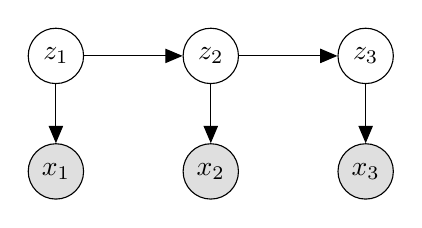
\begin{tikzpicture}[]
\node[latent] (z0) {$z_1$} ;
\node[latent] (z1) [right=1.25cm of z0] {$z_2$} ;
\node[latent] (z2) [right=1.25cm of z1] {$z_3$} ;

\node[obs]    (x0) [below = 0.75cm of z0] {$x_1$};
\node[obs]    (x1) [below = 0.75cm of z1] {$x_2$};
\node[obs]    (x2) [below = 0.75cm of z2] {$x_3$};

\edge {z0} {x0};
\edge {z1} {x1};
\edge {z2} {x2};
\edge {z0} {z1};
\edge {z1} {z2};
\end{tikzpicture}
\end{center}

This yields the joint distribution
$$p(x,z) = \prod_t p(x_t \mid z_t)p(z_t \mid z_{t-1})$$
%with distributional parameters
%\begin{align*}
%&\textnormal{start state vector } & \pi\in[0,1]^{Z},
%    & \textnormal{ with } &[\pi]_{z_0} &= p(z_0),\\
%&\textnormal{transition matrix } & A\in[0,1]^{Z \times Z},
%    & \textnormal{ with } &[A]_{z_{t-1},z_t} &= p(z_t \mid z_{t-1}),\\
%&\textnormal{emission matrix } & O\in[0,1]^{Z \times X},
%    & \textnormal{ with } &[O]_{z_t, x_t} &= p(x_t \mid z_t)\\
%\end{align*}
%
with 
\begin{align*}
&\textnormal{start state } & p(z_1)&,\\
&\textnormal{transitions } & p(z_t \mid z_{t-1})&,\\
&\textnormal{and emissions } &  p(x_t \mid z_t)&
\end{align*}
represented as vectors and matrices

\end{frame}



\begin{frame}
\frametitle{Inference}
Given observed $x = (x_1, \ldots, x_T)$
\vspace{1em}
We wish to maximize
\begin{equation*}
p(x)
= \sum_{z_1}\cdots\sum_{z_T}p(x, z)
= \alpha_1^\top\Lambda_2\Lambda_3\cdots\Lambda_T\bm1,
\end{equation*}
where we have the
\begin{align*}
&\textnormal{start, } & [\alpha_1]_{z_1} &= p(x_1\mid z_1)p(z_1),\\
&\textnormal{and transition operators, }
    & [\Lambda_t]_{z_{t-1},z_t} &= p(x_t \mid z_t)p(z_t \mid z_{t-1})
\end{align*}

\begin{itemize}
\item Matrix representation of forward algorithm:
$$\alpha_t = \alpha_{t-1}\Lambda_t$$
\item Requires $O(TZ^2)$ operations in total!
\end{itemize}
\end{frame}

\begin{comment}
\begin{frame}
\frametitle{Transition Operators}
skip slide? mainly to make the connection between distributional parameters
and inference really concrete.
\begin{itemize}
    \item The transition operators $\alpha_1,\Lambda_t$ are functions of
        the distributional parameters: starting state $\pi$, state transitions $A$,
            and emissions $O$
    \vspace{1em}
    \item In particular
\begin{align*}
&\textnormal{the start } & \alpha_1 &= \pi \circ [O]_{\cdot,x_1},\\
&\textnormal{and the transition operators }
    & \Lambda_t &= A\diag([O]_{\cdot, x_t})
\end{align*}
\end{itemize}
\end{frame}
\end{comment}

\begin{frame}
\frametitle{Inference}
%Given the start and transition operators, we can visualize inference
$$p(x) = \alpha_1^\top\Lambda_2\cdots\Lambda_T\mathbf{1}$$
\begin{figure}
\begin{center}
\resizebox{0.8\width}{0.8\height}{
\normalsize%
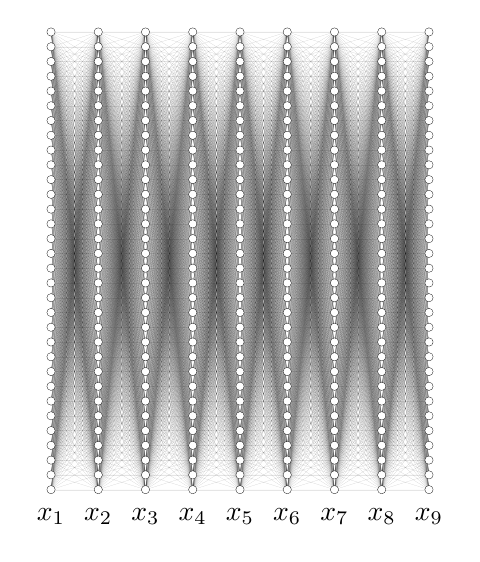
\begin{tikzpicture}%
\path[draw,line width=0.1pt,opacity=0.1,fill=black] (0.6,0.0) -- (1.2,0.0);%
\path[draw,line width=0.1pt,opacity=0.1,fill=black] (0.6,0.0) -- (1.2,0.1875);%
\path[draw,line width=0.1pt,opacity=0.1,fill=black] (0.6,0.0) -- (1.2,0.375);%
\path[draw,line width=0.1pt,opacity=0.1,fill=black] (0.6,0.0) -- (1.2,0.5625);%
\path[draw,line width=0.1pt,opacity=0.1,fill=black] (0.6,0.0) -- (1.2,0.75);%
\path[draw,line width=0.1pt,opacity=0.1,fill=black] (0.6,0.0) -- (1.2,0.9375);%
\path[draw,line width=0.1pt,opacity=0.1,fill=black] (0.6,0.0) -- (1.2,1.125);%
\path[draw,line width=0.1pt,opacity=0.1,fill=black] (0.6,0.0) -- (1.2,1.3125);%
\path[draw,line width=0.1pt,opacity=0.1,fill=black] (0.6,0.0) -- (1.2,1.5);%
\path[draw,line width=0.1pt,opacity=0.1,fill=black] (0.6,0.0) -- (1.2,1.6875);%
\path[draw,line width=0.1pt,opacity=0.1,fill=black] (0.6,0.0) -- (1.2,1.875);%
\path[draw,line width=0.1pt,opacity=0.1,fill=black] (0.6,0.0) -- (1.2,2.0625);%
\path[draw,line width=0.1pt,opacity=0.1,fill=black] (0.6,0.0) -- (1.2,2.25);%
\path[draw,line width=0.1pt,opacity=0.1,fill=black] (0.6,0.0) -- (1.2,2.4375);%
\path[draw,line width=0.1pt,opacity=0.1,fill=black] (0.6,0.0) -- (1.2,2.625);%
\path[draw,line width=0.1pt,opacity=0.1,fill=black] (0.6,0.0) -- (1.2,2.8125);%
\path[draw,line width=0.1pt,opacity=0.1,fill=black] (0.6,0.0) -- (1.2,3.0);%
\path[draw,line width=0.1pt,opacity=0.1,fill=black] (0.6,0.0) -- (1.2,3.1875);%
\path[draw,line width=0.1pt,opacity=0.1,fill=black] (0.6,0.0) -- (1.2,3.375);%
\path[draw,line width=0.1pt,opacity=0.1,fill=black] (0.6,0.0) -- (1.2,3.5625);%
\path[draw,line width=0.1pt,opacity=0.1,fill=black] (0.6,0.0) -- (1.2,3.75);%
\path[draw,line width=0.1pt,opacity=0.1,fill=black] (0.6,0.0) -- (1.2,3.9375);%
\path[draw,line width=0.1pt,opacity=0.1,fill=black] (0.6,0.0) -- (1.2,4.125);%
\path[draw,line width=0.1pt,opacity=0.1,fill=black] (0.6,0.0) -- (1.2,4.3125);%
\path[draw,line width=0.1pt,opacity=0.1,fill=black] (0.6,0.0) -- (1.2,4.5);%
\path[draw,line width=0.1pt,opacity=0.1,fill=black] (0.6,0.0) -- (1.2,4.6875);%
\path[draw,line width=0.1pt,opacity=0.1,fill=black] (0.6,0.0) -- (1.2,4.875);%
\path[draw,line width=0.1pt,opacity=0.1,fill=black] (0.6,0.0) -- (1.2,5.0625);%
\path[draw,line width=0.1pt,opacity=0.1,fill=black] (0.6,0.0) -- (1.2,5.25);%
\path[draw,line width=0.1pt,opacity=0.1,fill=black] (0.6,0.0) -- (1.2,5.4375);%
\path[draw,line width=0.1pt,opacity=0.1,fill=black] (0.6,0.0) -- (1.2,5.625);%
\path[draw,line width=0.1pt,opacity=0.1,fill=black] (0.6,0.0) -- (1.2,5.8125);%
\path[draw,line width=0.1pt,opacity=0.1,fill=black] (0.6,0.1875) -- (1.2,0.0);%
\path[draw,line width=0.1pt,opacity=0.1,fill=black] (0.6,0.1875) -- (1.2,0.1875);%
\path[draw,line width=0.1pt,opacity=0.1,fill=black] (0.6,0.1875) -- (1.2,0.375);%
\path[draw,line width=0.1pt,opacity=0.1,fill=black] (0.6,0.1875) -- (1.2,0.5625);%
\path[draw,line width=0.1pt,opacity=0.1,fill=black] (0.6,0.1875) -- (1.2,0.75);%
\path[draw,line width=0.1pt,opacity=0.1,fill=black] (0.6,0.1875) -- (1.2,0.9375);%
\path[draw,line width=0.1pt,opacity=0.1,fill=black] (0.6,0.1875) -- (1.2,1.125);%
\path[draw,line width=0.1pt,opacity=0.1,fill=black] (0.6,0.1875) -- (1.2,1.3125);%
\path[draw,line width=0.1pt,opacity=0.1,fill=black] (0.6,0.1875) -- (1.2,1.5);%
\path[draw,line width=0.1pt,opacity=0.1,fill=black] (0.6,0.1875) -- (1.2,1.6875);%
\path[draw,line width=0.1pt,opacity=0.1,fill=black] (0.6,0.1875) -- (1.2,1.875);%
\path[draw,line width=0.1pt,opacity=0.1,fill=black] (0.6,0.1875) -- (1.2,2.0625);%
\path[draw,line width=0.1pt,opacity=0.1,fill=black] (0.6,0.1875) -- (1.2,2.25);%
\path[draw,line width=0.1pt,opacity=0.1,fill=black] (0.6,0.1875) -- (1.2,2.4375);%
\path[draw,line width=0.1pt,opacity=0.1,fill=black] (0.6,0.1875) -- (1.2,2.625);%
\path[draw,line width=0.1pt,opacity=0.1,fill=black] (0.6,0.1875) -- (1.2,2.8125);%
\path[draw,line width=0.1pt,opacity=0.1,fill=black] (0.6,0.1875) -- (1.2,3.0);%
\path[draw,line width=0.1pt,opacity=0.1,fill=black] (0.6,0.1875) -- (1.2,3.1875);%
\path[draw,line width=0.1pt,opacity=0.1,fill=black] (0.6,0.1875) -- (1.2,3.375);%
\path[draw,line width=0.1pt,opacity=0.1,fill=black] (0.6,0.1875) -- (1.2,3.5625);%
\path[draw,line width=0.1pt,opacity=0.1,fill=black] (0.6,0.1875) -- (1.2,3.75);%
\path[draw,line width=0.1pt,opacity=0.1,fill=black] (0.6,0.1875) -- (1.2,3.9375);%
\path[draw,line width=0.1pt,opacity=0.1,fill=black] (0.6,0.1875) -- (1.2,4.125);%
\path[draw,line width=0.1pt,opacity=0.1,fill=black] (0.6,0.1875) -- (1.2,4.3125);%
\path[draw,line width=0.1pt,opacity=0.1,fill=black] (0.6,0.1875) -- (1.2,4.5);%
\path[draw,line width=0.1pt,opacity=0.1,fill=black] (0.6,0.1875) -- (1.2,4.6875);%
\path[draw,line width=0.1pt,opacity=0.1,fill=black] (0.6,0.1875) -- (1.2,4.875);%
\path[draw,line width=0.1pt,opacity=0.1,fill=black] (0.6,0.1875) -- (1.2,5.0625);%
\path[draw,line width=0.1pt,opacity=0.1,fill=black] (0.6,0.1875) -- (1.2,5.25);%
\path[draw,line width=0.1pt,opacity=0.1,fill=black] (0.6,0.1875) -- (1.2,5.4375);%
\path[draw,line width=0.1pt,opacity=0.1,fill=black] (0.6,0.1875) -- (1.2,5.625);%
\path[draw,line width=0.1pt,opacity=0.1,fill=black] (0.6,0.1875) -- (1.2,5.8125);%
\path[draw,line width=0.1pt,opacity=0.1,fill=black] (0.6,0.375) -- (1.2,0.0);%
\path[draw,line width=0.1pt,opacity=0.1,fill=black] (0.6,0.375) -- (1.2,0.1875);%
\path[draw,line width=0.1pt,opacity=0.1,fill=black] (0.6,0.375) -- (1.2,0.375);%
\path[draw,line width=0.1pt,opacity=0.1,fill=black] (0.6,0.375) -- (1.2,0.5625);%
\path[draw,line width=0.1pt,opacity=0.1,fill=black] (0.6,0.375) -- (1.2,0.75);%
\path[draw,line width=0.1pt,opacity=0.1,fill=black] (0.6,0.375) -- (1.2,0.9375);%
\path[draw,line width=0.1pt,opacity=0.1,fill=black] (0.6,0.375) -- (1.2,1.125);%
\path[draw,line width=0.1pt,opacity=0.1,fill=black] (0.6,0.375) -- (1.2,1.3125);%
\path[draw,line width=0.1pt,opacity=0.1,fill=black] (0.6,0.375) -- (1.2,1.5);%
\path[draw,line width=0.1pt,opacity=0.1,fill=black] (0.6,0.375) -- (1.2,1.6875);%
\path[draw,line width=0.1pt,opacity=0.1,fill=black] (0.6,0.375) -- (1.2,1.875);%
\path[draw,line width=0.1pt,opacity=0.1,fill=black] (0.6,0.375) -- (1.2,2.0625);%
\path[draw,line width=0.1pt,opacity=0.1,fill=black] (0.6,0.375) -- (1.2,2.25);%
\path[draw,line width=0.1pt,opacity=0.1,fill=black] (0.6,0.375) -- (1.2,2.4375);%
\path[draw,line width=0.1pt,opacity=0.1,fill=black] (0.6,0.375) -- (1.2,2.625);%
\path[draw,line width=0.1pt,opacity=0.1,fill=black] (0.6,0.375) -- (1.2,2.8125);%
\path[draw,line width=0.1pt,opacity=0.1,fill=black] (0.6,0.375) -- (1.2,3.0);%
\path[draw,line width=0.1pt,opacity=0.1,fill=black] (0.6,0.375) -- (1.2,3.1875);%
\path[draw,line width=0.1pt,opacity=0.1,fill=black] (0.6,0.375) -- (1.2,3.375);%
\path[draw,line width=0.1pt,opacity=0.1,fill=black] (0.6,0.375) -- (1.2,3.5625);%
\path[draw,line width=0.1pt,opacity=0.1,fill=black] (0.6,0.375) -- (1.2,3.75);%
\path[draw,line width=0.1pt,opacity=0.1,fill=black] (0.6,0.375) -- (1.2,3.9375);%
\path[draw,line width=0.1pt,opacity=0.1,fill=black] (0.6,0.375) -- (1.2,4.125);%
\path[draw,line width=0.1pt,opacity=0.1,fill=black] (0.6,0.375) -- (1.2,4.3125);%
\path[draw,line width=0.1pt,opacity=0.1,fill=black] (0.6,0.375) -- (1.2,4.5);%
\path[draw,line width=0.1pt,opacity=0.1,fill=black] (0.6,0.375) -- (1.2,4.6875);%
\path[draw,line width=0.1pt,opacity=0.1,fill=black] (0.6,0.375) -- (1.2,4.875);%
\path[draw,line width=0.1pt,opacity=0.1,fill=black] (0.6,0.375) -- (1.2,5.0625);%
\path[draw,line width=0.1pt,opacity=0.1,fill=black] (0.6,0.375) -- (1.2,5.25);%
\path[draw,line width=0.1pt,opacity=0.1,fill=black] (0.6,0.375) -- (1.2,5.4375);%
\path[draw,line width=0.1pt,opacity=0.1,fill=black] (0.6,0.375) -- (1.2,5.625);%
\path[draw,line width=0.1pt,opacity=0.1,fill=black] (0.6,0.375) -- (1.2,5.8125);%
\path[draw,line width=0.1pt,opacity=0.1,fill=black] (0.6,0.5625) -- (1.2,0.0);%
\path[draw,line width=0.1pt,opacity=0.1,fill=black] (0.6,0.5625) -- (1.2,0.1875);%
\path[draw,line width=0.1pt,opacity=0.1,fill=black] (0.6,0.5625) -- (1.2,0.375);%
\path[draw,line width=0.1pt,opacity=0.1,fill=black] (0.6,0.5625) -- (1.2,0.5625);%
\path[draw,line width=0.1pt,opacity=0.1,fill=black] (0.6,0.5625) -- (1.2,0.75);%
\path[draw,line width=0.1pt,opacity=0.1,fill=black] (0.6,0.5625) -- (1.2,0.9375);%
\path[draw,line width=0.1pt,opacity=0.1,fill=black] (0.6,0.5625) -- (1.2,1.125);%
\path[draw,line width=0.1pt,opacity=0.1,fill=black] (0.6,0.5625) -- (1.2,1.3125);%
\path[draw,line width=0.1pt,opacity=0.1,fill=black] (0.6,0.5625) -- (1.2,1.5);%
\path[draw,line width=0.1pt,opacity=0.1,fill=black] (0.6,0.5625) -- (1.2,1.6875);%
\path[draw,line width=0.1pt,opacity=0.1,fill=black] (0.6,0.5625) -- (1.2,1.875);%
\path[draw,line width=0.1pt,opacity=0.1,fill=black] (0.6,0.5625) -- (1.2,2.0625);%
\path[draw,line width=0.1pt,opacity=0.1,fill=black] (0.6,0.5625) -- (1.2,2.25);%
\path[draw,line width=0.1pt,opacity=0.1,fill=black] (0.6,0.5625) -- (1.2,2.4375);%
\path[draw,line width=0.1pt,opacity=0.1,fill=black] (0.6,0.5625) -- (1.2,2.625);%
\path[draw,line width=0.1pt,opacity=0.1,fill=black] (0.6,0.5625) -- (1.2,2.8125);%
\path[draw,line width=0.1pt,opacity=0.1,fill=black] (0.6,0.5625) -- (1.2,3.0);%
\path[draw,line width=0.1pt,opacity=0.1,fill=black] (0.6,0.5625) -- (1.2,3.1875);%
\path[draw,line width=0.1pt,opacity=0.1,fill=black] (0.6,0.5625) -- (1.2,3.375);%
\path[draw,line width=0.1pt,opacity=0.1,fill=black] (0.6,0.5625) -- (1.2,3.5625);%
\path[draw,line width=0.1pt,opacity=0.1,fill=black] (0.6,0.5625) -- (1.2,3.75);%
\path[draw,line width=0.1pt,opacity=0.1,fill=black] (0.6,0.5625) -- (1.2,3.9375);%
\path[draw,line width=0.1pt,opacity=0.1,fill=black] (0.6,0.5625) -- (1.2,4.125);%
\path[draw,line width=0.1pt,opacity=0.1,fill=black] (0.6,0.5625) -- (1.2,4.3125);%
\path[draw,line width=0.1pt,opacity=0.1,fill=black] (0.6,0.5625) -- (1.2,4.5);%
\path[draw,line width=0.1pt,opacity=0.1,fill=black] (0.6,0.5625) -- (1.2,4.6875);%
\path[draw,line width=0.1pt,opacity=0.1,fill=black] (0.6,0.5625) -- (1.2,4.875);%
\path[draw,line width=0.1pt,opacity=0.1,fill=black] (0.6,0.5625) -- (1.2,5.0625);%
\path[draw,line width=0.1pt,opacity=0.1,fill=black] (0.6,0.5625) -- (1.2,5.25);%
\path[draw,line width=0.1pt,opacity=0.1,fill=black] (0.6,0.5625) -- (1.2,5.4375);%
\path[draw,line width=0.1pt,opacity=0.1,fill=black] (0.6,0.5625) -- (1.2,5.625);%
\path[draw,line width=0.1pt,opacity=0.1,fill=black] (0.6,0.5625) -- (1.2,5.8125);%
\path[draw,line width=0.1pt,opacity=0.1,fill=black] (0.6,0.75) -- (1.2,0.0);%
\path[draw,line width=0.1pt,opacity=0.1,fill=black] (0.6,0.75) -- (1.2,0.1875);%
\path[draw,line width=0.1pt,opacity=0.1,fill=black] (0.6,0.75) -- (1.2,0.375);%
\path[draw,line width=0.1pt,opacity=0.1,fill=black] (0.6,0.75) -- (1.2,0.5625);%
\path[draw,line width=0.1pt,opacity=0.1,fill=black] (0.6,0.75) -- (1.2,0.75);%
\path[draw,line width=0.1pt,opacity=0.1,fill=black] (0.6,0.75) -- (1.2,0.9375);%
\path[draw,line width=0.1pt,opacity=0.1,fill=black] (0.6,0.75) -- (1.2,1.125);%
\path[draw,line width=0.1pt,opacity=0.1,fill=black] (0.6,0.75) -- (1.2,1.3125);%
\path[draw,line width=0.1pt,opacity=0.1,fill=black] (0.6,0.75) -- (1.2,1.5);%
\path[draw,line width=0.1pt,opacity=0.1,fill=black] (0.6,0.75) -- (1.2,1.6875);%
\path[draw,line width=0.1pt,opacity=0.1,fill=black] (0.6,0.75) -- (1.2,1.875);%
\path[draw,line width=0.1pt,opacity=0.1,fill=black] (0.6,0.75) -- (1.2,2.0625);%
\path[draw,line width=0.1pt,opacity=0.1,fill=black] (0.6,0.75) -- (1.2,2.25);%
\path[draw,line width=0.1pt,opacity=0.1,fill=black] (0.6,0.75) -- (1.2,2.4375);%
\path[draw,line width=0.1pt,opacity=0.1,fill=black] (0.6,0.75) -- (1.2,2.625);%
\path[draw,line width=0.1pt,opacity=0.1,fill=black] (0.6,0.75) -- (1.2,2.8125);%
\path[draw,line width=0.1pt,opacity=0.1,fill=black] (0.6,0.75) -- (1.2,3.0);%
\path[draw,line width=0.1pt,opacity=0.1,fill=black] (0.6,0.75) -- (1.2,3.1875);%
\path[draw,line width=0.1pt,opacity=0.1,fill=black] (0.6,0.75) -- (1.2,3.375);%
\path[draw,line width=0.1pt,opacity=0.1,fill=black] (0.6,0.75) -- (1.2,3.5625);%
\path[draw,line width=0.1pt,opacity=0.1,fill=black] (0.6,0.75) -- (1.2,3.75);%
\path[draw,line width=0.1pt,opacity=0.1,fill=black] (0.6,0.75) -- (1.2,3.9375);%
\path[draw,line width=0.1pt,opacity=0.1,fill=black] (0.6,0.75) -- (1.2,4.125);%
\path[draw,line width=0.1pt,opacity=0.1,fill=black] (0.6,0.75) -- (1.2,4.3125);%
\path[draw,line width=0.1pt,opacity=0.1,fill=black] (0.6,0.75) -- (1.2,4.5);%
\path[draw,line width=0.1pt,opacity=0.1,fill=black] (0.6,0.75) -- (1.2,4.6875);%
\path[draw,line width=0.1pt,opacity=0.1,fill=black] (0.6,0.75) -- (1.2,4.875);%
\path[draw,line width=0.1pt,opacity=0.1,fill=black] (0.6,0.75) -- (1.2,5.0625);%
\path[draw,line width=0.1pt,opacity=0.1,fill=black] (0.6,0.75) -- (1.2,5.25);%
\path[draw,line width=0.1pt,opacity=0.1,fill=black] (0.6,0.75) -- (1.2,5.4375);%
\path[draw,line width=0.1pt,opacity=0.1,fill=black] (0.6,0.75) -- (1.2,5.625);%
\path[draw,line width=0.1pt,opacity=0.1,fill=black] (0.6,0.75) -- (1.2,5.8125);%
\path[draw,line width=0.1pt,opacity=0.1,fill=black] (0.6,0.9375) -- (1.2,0.0);%
\path[draw,line width=0.1pt,opacity=0.1,fill=black] (0.6,0.9375) -- (1.2,0.1875);%
\path[draw,line width=0.1pt,opacity=0.1,fill=black] (0.6,0.9375) -- (1.2,0.375);%
\path[draw,line width=0.1pt,opacity=0.1,fill=black] (0.6,0.9375) -- (1.2,0.5625);%
\path[draw,line width=0.1pt,opacity=0.1,fill=black] (0.6,0.9375) -- (1.2,0.75);%
\path[draw,line width=0.1pt,opacity=0.1,fill=black] (0.6,0.9375) -- (1.2,0.9375);%
\path[draw,line width=0.1pt,opacity=0.1,fill=black] (0.6,0.9375) -- (1.2,1.125);%
\path[draw,line width=0.1pt,opacity=0.1,fill=black] (0.6,0.9375) -- (1.2,1.3125);%
\path[draw,line width=0.1pt,opacity=0.1,fill=black] (0.6,0.9375) -- (1.2,1.5);%
\path[draw,line width=0.1pt,opacity=0.1,fill=black] (0.6,0.9375) -- (1.2,1.6875);%
\path[draw,line width=0.1pt,opacity=0.1,fill=black] (0.6,0.9375) -- (1.2,1.875);%
\path[draw,line width=0.1pt,opacity=0.1,fill=black] (0.6,0.9375) -- (1.2,2.0625);%
\path[draw,line width=0.1pt,opacity=0.1,fill=black] (0.6,0.9375) -- (1.2,2.25);%
\path[draw,line width=0.1pt,opacity=0.1,fill=black] (0.6,0.9375) -- (1.2,2.4375);%
\path[draw,line width=0.1pt,opacity=0.1,fill=black] (0.6,0.9375) -- (1.2,2.625);%
\path[draw,line width=0.1pt,opacity=0.1,fill=black] (0.6,0.9375) -- (1.2,2.8125);%
\path[draw,line width=0.1pt,opacity=0.1,fill=black] (0.6,0.9375) -- (1.2,3.0);%
\path[draw,line width=0.1pt,opacity=0.1,fill=black] (0.6,0.9375) -- (1.2,3.1875);%
\path[draw,line width=0.1pt,opacity=0.1,fill=black] (0.6,0.9375) -- (1.2,3.375);%
\path[draw,line width=0.1pt,opacity=0.1,fill=black] (0.6,0.9375) -- (1.2,3.5625);%
\path[draw,line width=0.1pt,opacity=0.1,fill=black] (0.6,0.9375) -- (1.2,3.75);%
\path[draw,line width=0.1pt,opacity=0.1,fill=black] (0.6,0.9375) -- (1.2,3.9375);%
\path[draw,line width=0.1pt,opacity=0.1,fill=black] (0.6,0.9375) -- (1.2,4.125);%
\path[draw,line width=0.1pt,opacity=0.1,fill=black] (0.6,0.9375) -- (1.2,4.3125);%
\path[draw,line width=0.1pt,opacity=0.1,fill=black] (0.6,0.9375) -- (1.2,4.5);%
\path[draw,line width=0.1pt,opacity=0.1,fill=black] (0.6,0.9375) -- (1.2,4.6875);%
\path[draw,line width=0.1pt,opacity=0.1,fill=black] (0.6,0.9375) -- (1.2,4.875);%
\path[draw,line width=0.1pt,opacity=0.1,fill=black] (0.6,0.9375) -- (1.2,5.0625);%
\path[draw,line width=0.1pt,opacity=0.1,fill=black] (0.6,0.9375) -- (1.2,5.25);%
\path[draw,line width=0.1pt,opacity=0.1,fill=black] (0.6,0.9375) -- (1.2,5.4375);%
\path[draw,line width=0.1pt,opacity=0.1,fill=black] (0.6,0.9375) -- (1.2,5.625);%
\path[draw,line width=0.1pt,opacity=0.1,fill=black] (0.6,0.9375) -- (1.2,5.8125);%
\path[draw,line width=0.1pt,opacity=0.1,fill=black] (0.6,1.125) -- (1.2,0.0);%
\path[draw,line width=0.1pt,opacity=0.1,fill=black] (0.6,1.125) -- (1.2,0.1875);%
\path[draw,line width=0.1pt,opacity=0.1,fill=black] (0.6,1.125) -- (1.2,0.375);%
\path[draw,line width=0.1pt,opacity=0.1,fill=black] (0.6,1.125) -- (1.2,0.5625);%
\path[draw,line width=0.1pt,opacity=0.1,fill=black] (0.6,1.125) -- (1.2,0.75);%
\path[draw,line width=0.1pt,opacity=0.1,fill=black] (0.6,1.125) -- (1.2,0.9375);%
\path[draw,line width=0.1pt,opacity=0.1,fill=black] (0.6,1.125) -- (1.2,1.125);%
\path[draw,line width=0.1pt,opacity=0.1,fill=black] (0.6,1.125) -- (1.2,1.3125);%
\path[draw,line width=0.1pt,opacity=0.1,fill=black] (0.6,1.125) -- (1.2,1.5);%
\path[draw,line width=0.1pt,opacity=0.1,fill=black] (0.6,1.125) -- (1.2,1.6875);%
\path[draw,line width=0.1pt,opacity=0.1,fill=black] (0.6,1.125) -- (1.2,1.875);%
\path[draw,line width=0.1pt,opacity=0.1,fill=black] (0.6,1.125) -- (1.2,2.0625);%
\path[draw,line width=0.1pt,opacity=0.1,fill=black] (0.6,1.125) -- (1.2,2.25);%
\path[draw,line width=0.1pt,opacity=0.1,fill=black] (0.6,1.125) -- (1.2,2.4375);%
\path[draw,line width=0.1pt,opacity=0.1,fill=black] (0.6,1.125) -- (1.2,2.625);%
\path[draw,line width=0.1pt,opacity=0.1,fill=black] (0.6,1.125) -- (1.2,2.8125);%
\path[draw,line width=0.1pt,opacity=0.1,fill=black] (0.6,1.125) -- (1.2,3.0);%
\path[draw,line width=0.1pt,opacity=0.1,fill=black] (0.6,1.125) -- (1.2,3.1875);%
\path[draw,line width=0.1pt,opacity=0.1,fill=black] (0.6,1.125) -- (1.2,3.375);%
\path[draw,line width=0.1pt,opacity=0.1,fill=black] (0.6,1.125) -- (1.2,3.5625);%
\path[draw,line width=0.1pt,opacity=0.1,fill=black] (0.6,1.125) -- (1.2,3.75);%
\path[draw,line width=0.1pt,opacity=0.1,fill=black] (0.6,1.125) -- (1.2,3.9375);%
\path[draw,line width=0.1pt,opacity=0.1,fill=black] (0.6,1.125) -- (1.2,4.125);%
\path[draw,line width=0.1pt,opacity=0.1,fill=black] (0.6,1.125) -- (1.2,4.3125);%
\path[draw,line width=0.1pt,opacity=0.1,fill=black] (0.6,1.125) -- (1.2,4.5);%
\path[draw,line width=0.1pt,opacity=0.1,fill=black] (0.6,1.125) -- (1.2,4.6875);%
\path[draw,line width=0.1pt,opacity=0.1,fill=black] (0.6,1.125) -- (1.2,4.875);%
\path[draw,line width=0.1pt,opacity=0.1,fill=black] (0.6,1.125) -- (1.2,5.0625);%
\path[draw,line width=0.1pt,opacity=0.1,fill=black] (0.6,1.125) -- (1.2,5.25);%
\path[draw,line width=0.1pt,opacity=0.1,fill=black] (0.6,1.125) -- (1.2,5.4375);%
\path[draw,line width=0.1pt,opacity=0.1,fill=black] (0.6,1.125) -- (1.2,5.625);%
\path[draw,line width=0.1pt,opacity=0.1,fill=black] (0.6,1.125) -- (1.2,5.8125);%
\path[draw,line width=0.1pt,opacity=0.1,fill=black] (0.6,1.3125) -- (1.2,0.0);%
\path[draw,line width=0.1pt,opacity=0.1,fill=black] (0.6,1.3125) -- (1.2,0.1875);%
\path[draw,line width=0.1pt,opacity=0.1,fill=black] (0.6,1.3125) -- (1.2,0.375);%
\path[draw,line width=0.1pt,opacity=0.1,fill=black] (0.6,1.3125) -- (1.2,0.5625);%
\path[draw,line width=0.1pt,opacity=0.1,fill=black] (0.6,1.3125) -- (1.2,0.75);%
\path[draw,line width=0.1pt,opacity=0.1,fill=black] (0.6,1.3125) -- (1.2,0.9375);%
\path[draw,line width=0.1pt,opacity=0.1,fill=black] (0.6,1.3125) -- (1.2,1.125);%
\path[draw,line width=0.1pt,opacity=0.1,fill=black] (0.6,1.3125) -- (1.2,1.3125);%
\path[draw,line width=0.1pt,opacity=0.1,fill=black] (0.6,1.3125) -- (1.2,1.5);%
\path[draw,line width=0.1pt,opacity=0.1,fill=black] (0.6,1.3125) -- (1.2,1.6875);%
\path[draw,line width=0.1pt,opacity=0.1,fill=black] (0.6,1.3125) -- (1.2,1.875);%
\path[draw,line width=0.1pt,opacity=0.1,fill=black] (0.6,1.3125) -- (1.2,2.0625);%
\path[draw,line width=0.1pt,opacity=0.1,fill=black] (0.6,1.3125) -- (1.2,2.25);%
\path[draw,line width=0.1pt,opacity=0.1,fill=black] (0.6,1.3125) -- (1.2,2.4375);%
\path[draw,line width=0.1pt,opacity=0.1,fill=black] (0.6,1.3125) -- (1.2,2.625);%
\path[draw,line width=0.1pt,opacity=0.1,fill=black] (0.6,1.3125) -- (1.2,2.8125);%
\path[draw,line width=0.1pt,opacity=0.1,fill=black] (0.6,1.3125) -- (1.2,3.0);%
\path[draw,line width=0.1pt,opacity=0.1,fill=black] (0.6,1.3125) -- (1.2,3.1875);%
\path[draw,line width=0.1pt,opacity=0.1,fill=black] (0.6,1.3125) -- (1.2,3.375);%
\path[draw,line width=0.1pt,opacity=0.1,fill=black] (0.6,1.3125) -- (1.2,3.5625);%
\path[draw,line width=0.1pt,opacity=0.1,fill=black] (0.6,1.3125) -- (1.2,3.75);%
\path[draw,line width=0.1pt,opacity=0.1,fill=black] (0.6,1.3125) -- (1.2,3.9375);%
\path[draw,line width=0.1pt,opacity=0.1,fill=black] (0.6,1.3125) -- (1.2,4.125);%
\path[draw,line width=0.1pt,opacity=0.1,fill=black] (0.6,1.3125) -- (1.2,4.3125);%
\path[draw,line width=0.1pt,opacity=0.1,fill=black] (0.6,1.3125) -- (1.2,4.5);%
\path[draw,line width=0.1pt,opacity=0.1,fill=black] (0.6,1.3125) -- (1.2,4.6875);%
\path[draw,line width=0.1pt,opacity=0.1,fill=black] (0.6,1.3125) -- (1.2,4.875);%
\path[draw,line width=0.1pt,opacity=0.1,fill=black] (0.6,1.3125) -- (1.2,5.0625);%
\path[draw,line width=0.1pt,opacity=0.1,fill=black] (0.6,1.3125) -- (1.2,5.25);%
\path[draw,line width=0.1pt,opacity=0.1,fill=black] (0.6,1.3125) -- (1.2,5.4375);%
\path[draw,line width=0.1pt,opacity=0.1,fill=black] (0.6,1.3125) -- (1.2,5.625);%
\path[draw,line width=0.1pt,opacity=0.1,fill=black] (0.6,1.3125) -- (1.2,5.8125);%
\path[draw,line width=0.1pt,opacity=0.1,fill=black] (0.6,1.5) -- (1.2,0.0);%
\path[draw,line width=0.1pt,opacity=0.1,fill=black] (0.6,1.5) -- (1.2,0.1875);%
\path[draw,line width=0.1pt,opacity=0.1,fill=black] (0.6,1.5) -- (1.2,0.375);%
\path[draw,line width=0.1pt,opacity=0.1,fill=black] (0.6,1.5) -- (1.2,0.5625);%
\path[draw,line width=0.1pt,opacity=0.1,fill=black] (0.6,1.5) -- (1.2,0.75);%
\path[draw,line width=0.1pt,opacity=0.1,fill=black] (0.6,1.5) -- (1.2,0.9375);%
\path[draw,line width=0.1pt,opacity=0.1,fill=black] (0.6,1.5) -- (1.2,1.125);%
\path[draw,line width=0.1pt,opacity=0.1,fill=black] (0.6,1.5) -- (1.2,1.3125);%
\path[draw,line width=0.1pt,opacity=0.1,fill=black] (0.6,1.5) -- (1.2,1.5);%
\path[draw,line width=0.1pt,opacity=0.1,fill=black] (0.6,1.5) -- (1.2,1.6875);%
\path[draw,line width=0.1pt,opacity=0.1,fill=black] (0.6,1.5) -- (1.2,1.875);%
\path[draw,line width=0.1pt,opacity=0.1,fill=black] (0.6,1.5) -- (1.2,2.0625);%
\path[draw,line width=0.1pt,opacity=0.1,fill=black] (0.6,1.5) -- (1.2,2.25);%
\path[draw,line width=0.1pt,opacity=0.1,fill=black] (0.6,1.5) -- (1.2,2.4375);%
\path[draw,line width=0.1pt,opacity=0.1,fill=black] (0.6,1.5) -- (1.2,2.625);%
\path[draw,line width=0.1pt,opacity=0.1,fill=black] (0.6,1.5) -- (1.2,2.8125);%
\path[draw,line width=0.1pt,opacity=0.1,fill=black] (0.6,1.5) -- (1.2,3.0);%
\path[draw,line width=0.1pt,opacity=0.1,fill=black] (0.6,1.5) -- (1.2,3.1875);%
\path[draw,line width=0.1pt,opacity=0.1,fill=black] (0.6,1.5) -- (1.2,3.375);%
\path[draw,line width=0.1pt,opacity=0.1,fill=black] (0.6,1.5) -- (1.2,3.5625);%
\path[draw,line width=0.1pt,opacity=0.1,fill=black] (0.6,1.5) -- (1.2,3.75);%
\path[draw,line width=0.1pt,opacity=0.1,fill=black] (0.6,1.5) -- (1.2,3.9375);%
\path[draw,line width=0.1pt,opacity=0.1,fill=black] (0.6,1.5) -- (1.2,4.125);%
\path[draw,line width=0.1pt,opacity=0.1,fill=black] (0.6,1.5) -- (1.2,4.3125);%
\path[draw,line width=0.1pt,opacity=0.1,fill=black] (0.6,1.5) -- (1.2,4.5);%
\path[draw,line width=0.1pt,opacity=0.1,fill=black] (0.6,1.5) -- (1.2,4.6875);%
\path[draw,line width=0.1pt,opacity=0.1,fill=black] (0.6,1.5) -- (1.2,4.875);%
\path[draw,line width=0.1pt,opacity=0.1,fill=black] (0.6,1.5) -- (1.2,5.0625);%
\path[draw,line width=0.1pt,opacity=0.1,fill=black] (0.6,1.5) -- (1.2,5.25);%
\path[draw,line width=0.1pt,opacity=0.1,fill=black] (0.6,1.5) -- (1.2,5.4375);%
\path[draw,line width=0.1pt,opacity=0.1,fill=black] (0.6,1.5) -- (1.2,5.625);%
\path[draw,line width=0.1pt,opacity=0.1,fill=black] (0.6,1.5) -- (1.2,5.8125);%
\path[draw,line width=0.1pt,opacity=0.1,fill=black] (0.6,1.6875) -- (1.2,0.0);%
\path[draw,line width=0.1pt,opacity=0.1,fill=black] (0.6,1.6875) -- (1.2,0.1875);%
\path[draw,line width=0.1pt,opacity=0.1,fill=black] (0.6,1.6875) -- (1.2,0.375);%
\path[draw,line width=0.1pt,opacity=0.1,fill=black] (0.6,1.6875) -- (1.2,0.5625);%
\path[draw,line width=0.1pt,opacity=0.1,fill=black] (0.6,1.6875) -- (1.2,0.75);%
\path[draw,line width=0.1pt,opacity=0.1,fill=black] (0.6,1.6875) -- (1.2,0.9375);%
\path[draw,line width=0.1pt,opacity=0.1,fill=black] (0.6,1.6875) -- (1.2,1.125);%
\path[draw,line width=0.1pt,opacity=0.1,fill=black] (0.6,1.6875) -- (1.2,1.3125);%
\path[draw,line width=0.1pt,opacity=0.1,fill=black] (0.6,1.6875) -- (1.2,1.5);%
\path[draw,line width=0.1pt,opacity=0.1,fill=black] (0.6,1.6875) -- (1.2,1.6875);%
\path[draw,line width=0.1pt,opacity=0.1,fill=black] (0.6,1.6875) -- (1.2,1.875);%
\path[draw,line width=0.1pt,opacity=0.1,fill=black] (0.6,1.6875) -- (1.2,2.0625);%
\path[draw,line width=0.1pt,opacity=0.1,fill=black] (0.6,1.6875) -- (1.2,2.25);%
\path[draw,line width=0.1pt,opacity=0.1,fill=black] (0.6,1.6875) -- (1.2,2.4375);%
\path[draw,line width=0.1pt,opacity=0.1,fill=black] (0.6,1.6875) -- (1.2,2.625);%
\path[draw,line width=0.1pt,opacity=0.1,fill=black] (0.6,1.6875) -- (1.2,2.8125);%
\path[draw,line width=0.1pt,opacity=0.1,fill=black] (0.6,1.6875) -- (1.2,3.0);%
\path[draw,line width=0.1pt,opacity=0.1,fill=black] (0.6,1.6875) -- (1.2,3.1875);%
\path[draw,line width=0.1pt,opacity=0.1,fill=black] (0.6,1.6875) -- (1.2,3.375);%
\path[draw,line width=0.1pt,opacity=0.1,fill=black] (0.6,1.6875) -- (1.2,3.5625);%
\path[draw,line width=0.1pt,opacity=0.1,fill=black] (0.6,1.6875) -- (1.2,3.75);%
\path[draw,line width=0.1pt,opacity=0.1,fill=black] (0.6,1.6875) -- (1.2,3.9375);%
\path[draw,line width=0.1pt,opacity=0.1,fill=black] (0.6,1.6875) -- (1.2,4.125);%
\path[draw,line width=0.1pt,opacity=0.1,fill=black] (0.6,1.6875) -- (1.2,4.3125);%
\path[draw,line width=0.1pt,opacity=0.1,fill=black] (0.6,1.6875) -- (1.2,4.5);%
\path[draw,line width=0.1pt,opacity=0.1,fill=black] (0.6,1.6875) -- (1.2,4.6875);%
\path[draw,line width=0.1pt,opacity=0.1,fill=black] (0.6,1.6875) -- (1.2,4.875);%
\path[draw,line width=0.1pt,opacity=0.1,fill=black] (0.6,1.6875) -- (1.2,5.0625);%
\path[draw,line width=0.1pt,opacity=0.1,fill=black] (0.6,1.6875) -- (1.2,5.25);%
\path[draw,line width=0.1pt,opacity=0.1,fill=black] (0.6,1.6875) -- (1.2,5.4375);%
\path[draw,line width=0.1pt,opacity=0.1,fill=black] (0.6,1.6875) -- (1.2,5.625);%
\path[draw,line width=0.1pt,opacity=0.1,fill=black] (0.6,1.6875) -- (1.2,5.8125);%
\path[draw,line width=0.1pt,opacity=0.1,fill=black] (0.6,1.875) -- (1.2,0.0);%
\path[draw,line width=0.1pt,opacity=0.1,fill=black] (0.6,1.875) -- (1.2,0.1875);%
\path[draw,line width=0.1pt,opacity=0.1,fill=black] (0.6,1.875) -- (1.2,0.375);%
\path[draw,line width=0.1pt,opacity=0.1,fill=black] (0.6,1.875) -- (1.2,0.5625);%
\path[draw,line width=0.1pt,opacity=0.1,fill=black] (0.6,1.875) -- (1.2,0.75);%
\path[draw,line width=0.1pt,opacity=0.1,fill=black] (0.6,1.875) -- (1.2,0.9375);%
\path[draw,line width=0.1pt,opacity=0.1,fill=black] (0.6,1.875) -- (1.2,1.125);%
\path[draw,line width=0.1pt,opacity=0.1,fill=black] (0.6,1.875) -- (1.2,1.3125);%
\path[draw,line width=0.1pt,opacity=0.1,fill=black] (0.6,1.875) -- (1.2,1.5);%
\path[draw,line width=0.1pt,opacity=0.1,fill=black] (0.6,1.875) -- (1.2,1.6875);%
\path[draw,line width=0.1pt,opacity=0.1,fill=black] (0.6,1.875) -- (1.2,1.875);%
\path[draw,line width=0.1pt,opacity=0.1,fill=black] (0.6,1.875) -- (1.2,2.0625);%
\path[draw,line width=0.1pt,opacity=0.1,fill=black] (0.6,1.875) -- (1.2,2.25);%
\path[draw,line width=0.1pt,opacity=0.1,fill=black] (0.6,1.875) -- (1.2,2.4375);%
\path[draw,line width=0.1pt,opacity=0.1,fill=black] (0.6,1.875) -- (1.2,2.625);%
\path[draw,line width=0.1pt,opacity=0.1,fill=black] (0.6,1.875) -- (1.2,2.8125);%
\path[draw,line width=0.1pt,opacity=0.1,fill=black] (0.6,1.875) -- (1.2,3.0);%
\path[draw,line width=0.1pt,opacity=0.1,fill=black] (0.6,1.875) -- (1.2,3.1875);%
\path[draw,line width=0.1pt,opacity=0.1,fill=black] (0.6,1.875) -- (1.2,3.375);%
\path[draw,line width=0.1pt,opacity=0.1,fill=black] (0.6,1.875) -- (1.2,3.5625);%
\path[draw,line width=0.1pt,opacity=0.1,fill=black] (0.6,1.875) -- (1.2,3.75);%
\path[draw,line width=0.1pt,opacity=0.1,fill=black] (0.6,1.875) -- (1.2,3.9375);%
\path[draw,line width=0.1pt,opacity=0.1,fill=black] (0.6,1.875) -- (1.2,4.125);%
\path[draw,line width=0.1pt,opacity=0.1,fill=black] (0.6,1.875) -- (1.2,4.3125);%
\path[draw,line width=0.1pt,opacity=0.1,fill=black] (0.6,1.875) -- (1.2,4.5);%
\path[draw,line width=0.1pt,opacity=0.1,fill=black] (0.6,1.875) -- (1.2,4.6875);%
\path[draw,line width=0.1pt,opacity=0.1,fill=black] (0.6,1.875) -- (1.2,4.875);%
\path[draw,line width=0.1pt,opacity=0.1,fill=black] (0.6,1.875) -- (1.2,5.0625);%
\path[draw,line width=0.1pt,opacity=0.1,fill=black] (0.6,1.875) -- (1.2,5.25);%
\path[draw,line width=0.1pt,opacity=0.1,fill=black] (0.6,1.875) -- (1.2,5.4375);%
\path[draw,line width=0.1pt,opacity=0.1,fill=black] (0.6,1.875) -- (1.2,5.625);%
\path[draw,line width=0.1pt,opacity=0.1,fill=black] (0.6,1.875) -- (1.2,5.8125);%
\path[draw,line width=0.1pt,opacity=0.1,fill=black] (0.6,2.0625) -- (1.2,0.0);%
\path[draw,line width=0.1pt,opacity=0.1,fill=black] (0.6,2.0625) -- (1.2,0.1875);%
\path[draw,line width=0.1pt,opacity=0.1,fill=black] (0.6,2.0625) -- (1.2,0.375);%
\path[draw,line width=0.1pt,opacity=0.1,fill=black] (0.6,2.0625) -- (1.2,0.5625);%
\path[draw,line width=0.1pt,opacity=0.1,fill=black] (0.6,2.0625) -- (1.2,0.75);%
\path[draw,line width=0.1pt,opacity=0.1,fill=black] (0.6,2.0625) -- (1.2,0.9375);%
\path[draw,line width=0.1pt,opacity=0.1,fill=black] (0.6,2.0625) -- (1.2,1.125);%
\path[draw,line width=0.1pt,opacity=0.1,fill=black] (0.6,2.0625) -- (1.2,1.3125);%
\path[draw,line width=0.1pt,opacity=0.1,fill=black] (0.6,2.0625) -- (1.2,1.5);%
\path[draw,line width=0.1pt,opacity=0.1,fill=black] (0.6,2.0625) -- (1.2,1.6875);%
\path[draw,line width=0.1pt,opacity=0.1,fill=black] (0.6,2.0625) -- (1.2,1.875);%
\path[draw,line width=0.1pt,opacity=0.1,fill=black] (0.6,2.0625) -- (1.2,2.0625);%
\path[draw,line width=0.1pt,opacity=0.1,fill=black] (0.6,2.0625) -- (1.2,2.25);%
\path[draw,line width=0.1pt,opacity=0.1,fill=black] (0.6,2.0625) -- (1.2,2.4375);%
\path[draw,line width=0.1pt,opacity=0.1,fill=black] (0.6,2.0625) -- (1.2,2.625);%
\path[draw,line width=0.1pt,opacity=0.1,fill=black] (0.6,2.0625) -- (1.2,2.8125);%
\path[draw,line width=0.1pt,opacity=0.1,fill=black] (0.6,2.0625) -- (1.2,3.0);%
\path[draw,line width=0.1pt,opacity=0.1,fill=black] (0.6,2.0625) -- (1.2,3.1875);%
\path[draw,line width=0.1pt,opacity=0.1,fill=black] (0.6,2.0625) -- (1.2,3.375);%
\path[draw,line width=0.1pt,opacity=0.1,fill=black] (0.6,2.0625) -- (1.2,3.5625);%
\path[draw,line width=0.1pt,opacity=0.1,fill=black] (0.6,2.0625) -- (1.2,3.75);%
\path[draw,line width=0.1pt,opacity=0.1,fill=black] (0.6,2.0625) -- (1.2,3.9375);%
\path[draw,line width=0.1pt,opacity=0.1,fill=black] (0.6,2.0625) -- (1.2,4.125);%
\path[draw,line width=0.1pt,opacity=0.1,fill=black] (0.6,2.0625) -- (1.2,4.3125);%
\path[draw,line width=0.1pt,opacity=0.1,fill=black] (0.6,2.0625) -- (1.2,4.5);%
\path[draw,line width=0.1pt,opacity=0.1,fill=black] (0.6,2.0625) -- (1.2,4.6875);%
\path[draw,line width=0.1pt,opacity=0.1,fill=black] (0.6,2.0625) -- (1.2,4.875);%
\path[draw,line width=0.1pt,opacity=0.1,fill=black] (0.6,2.0625) -- (1.2,5.0625);%
\path[draw,line width=0.1pt,opacity=0.1,fill=black] (0.6,2.0625) -- (1.2,5.25);%
\path[draw,line width=0.1pt,opacity=0.1,fill=black] (0.6,2.0625) -- (1.2,5.4375);%
\path[draw,line width=0.1pt,opacity=0.1,fill=black] (0.6,2.0625) -- (1.2,5.625);%
\path[draw,line width=0.1pt,opacity=0.1,fill=black] (0.6,2.0625) -- (1.2,5.8125);%
\path[draw,line width=0.1pt,opacity=0.1,fill=black] (0.6,2.25) -- (1.2,0.0);%
\path[draw,line width=0.1pt,opacity=0.1,fill=black] (0.6,2.25) -- (1.2,0.1875);%
\path[draw,line width=0.1pt,opacity=0.1,fill=black] (0.6,2.25) -- (1.2,0.375);%
\path[draw,line width=0.1pt,opacity=0.1,fill=black] (0.6,2.25) -- (1.2,0.5625);%
\path[draw,line width=0.1pt,opacity=0.1,fill=black] (0.6,2.25) -- (1.2,0.75);%
\path[draw,line width=0.1pt,opacity=0.1,fill=black] (0.6,2.25) -- (1.2,0.9375);%
\path[draw,line width=0.1pt,opacity=0.1,fill=black] (0.6,2.25) -- (1.2,1.125);%
\path[draw,line width=0.1pt,opacity=0.1,fill=black] (0.6,2.25) -- (1.2,1.3125);%
\path[draw,line width=0.1pt,opacity=0.1,fill=black] (0.6,2.25) -- (1.2,1.5);%
\path[draw,line width=0.1pt,opacity=0.1,fill=black] (0.6,2.25) -- (1.2,1.6875);%
\path[draw,line width=0.1pt,opacity=0.1,fill=black] (0.6,2.25) -- (1.2,1.875);%
\path[draw,line width=0.1pt,opacity=0.1,fill=black] (0.6,2.25) -- (1.2,2.0625);%
\path[draw,line width=0.1pt,opacity=0.1,fill=black] (0.6,2.25) -- (1.2,2.25);%
\path[draw,line width=0.1pt,opacity=0.1,fill=black] (0.6,2.25) -- (1.2,2.4375);%
\path[draw,line width=0.1pt,opacity=0.1,fill=black] (0.6,2.25) -- (1.2,2.625);%
\path[draw,line width=0.1pt,opacity=0.1,fill=black] (0.6,2.25) -- (1.2,2.8125);%
\path[draw,line width=0.1pt,opacity=0.1,fill=black] (0.6,2.25) -- (1.2,3.0);%
\path[draw,line width=0.1pt,opacity=0.1,fill=black] (0.6,2.25) -- (1.2,3.1875);%
\path[draw,line width=0.1pt,opacity=0.1,fill=black] (0.6,2.25) -- (1.2,3.375);%
\path[draw,line width=0.1pt,opacity=0.1,fill=black] (0.6,2.25) -- (1.2,3.5625);%
\path[draw,line width=0.1pt,opacity=0.1,fill=black] (0.6,2.25) -- (1.2,3.75);%
\path[draw,line width=0.1pt,opacity=0.1,fill=black] (0.6,2.25) -- (1.2,3.9375);%
\path[draw,line width=0.1pt,opacity=0.1,fill=black] (0.6,2.25) -- (1.2,4.125);%
\path[draw,line width=0.1pt,opacity=0.1,fill=black] (0.6,2.25) -- (1.2,4.3125);%
\path[draw,line width=0.1pt,opacity=0.1,fill=black] (0.6,2.25) -- (1.2,4.5);%
\path[draw,line width=0.1pt,opacity=0.1,fill=black] (0.6,2.25) -- (1.2,4.6875);%
\path[draw,line width=0.1pt,opacity=0.1,fill=black] (0.6,2.25) -- (1.2,4.875);%
\path[draw,line width=0.1pt,opacity=0.1,fill=black] (0.6,2.25) -- (1.2,5.0625);%
\path[draw,line width=0.1pt,opacity=0.1,fill=black] (0.6,2.25) -- (1.2,5.25);%
\path[draw,line width=0.1pt,opacity=0.1,fill=black] (0.6,2.25) -- (1.2,5.4375);%
\path[draw,line width=0.1pt,opacity=0.1,fill=black] (0.6,2.25) -- (1.2,5.625);%
\path[draw,line width=0.1pt,opacity=0.1,fill=black] (0.6,2.25) -- (1.2,5.8125);%
\path[draw,line width=0.1pt,opacity=0.1,fill=black] (0.6,2.4375) -- (1.2,0.0);%
\path[draw,line width=0.1pt,opacity=0.1,fill=black] (0.6,2.4375) -- (1.2,0.1875);%
\path[draw,line width=0.1pt,opacity=0.1,fill=black] (0.6,2.4375) -- (1.2,0.375);%
\path[draw,line width=0.1pt,opacity=0.1,fill=black] (0.6,2.4375) -- (1.2,0.5625);%
\path[draw,line width=0.1pt,opacity=0.1,fill=black] (0.6,2.4375) -- (1.2,0.75);%
\path[draw,line width=0.1pt,opacity=0.1,fill=black] (0.6,2.4375) -- (1.2,0.9375);%
\path[draw,line width=0.1pt,opacity=0.1,fill=black] (0.6,2.4375) -- (1.2,1.125);%
\path[draw,line width=0.1pt,opacity=0.1,fill=black] (0.6,2.4375) -- (1.2,1.3125);%
\path[draw,line width=0.1pt,opacity=0.1,fill=black] (0.6,2.4375) -- (1.2,1.5);%
\path[draw,line width=0.1pt,opacity=0.1,fill=black] (0.6,2.4375) -- (1.2,1.6875);%
\path[draw,line width=0.1pt,opacity=0.1,fill=black] (0.6,2.4375) -- (1.2,1.875);%
\path[draw,line width=0.1pt,opacity=0.1,fill=black] (0.6,2.4375) -- (1.2,2.0625);%
\path[draw,line width=0.1pt,opacity=0.1,fill=black] (0.6,2.4375) -- (1.2,2.25);%
\path[draw,line width=0.1pt,opacity=0.1,fill=black] (0.6,2.4375) -- (1.2,2.4375);%
\path[draw,line width=0.1pt,opacity=0.1,fill=black] (0.6,2.4375) -- (1.2,2.625);%
\path[draw,line width=0.1pt,opacity=0.1,fill=black] (0.6,2.4375) -- (1.2,2.8125);%
\path[draw,line width=0.1pt,opacity=0.1,fill=black] (0.6,2.4375) -- (1.2,3.0);%
\path[draw,line width=0.1pt,opacity=0.1,fill=black] (0.6,2.4375) -- (1.2,3.1875);%
\path[draw,line width=0.1pt,opacity=0.1,fill=black] (0.6,2.4375) -- (1.2,3.375);%
\path[draw,line width=0.1pt,opacity=0.1,fill=black] (0.6,2.4375) -- (1.2,3.5625);%
\path[draw,line width=0.1pt,opacity=0.1,fill=black] (0.6,2.4375) -- (1.2,3.75);%
\path[draw,line width=0.1pt,opacity=0.1,fill=black] (0.6,2.4375) -- (1.2,3.9375);%
\path[draw,line width=0.1pt,opacity=0.1,fill=black] (0.6,2.4375) -- (1.2,4.125);%
\path[draw,line width=0.1pt,opacity=0.1,fill=black] (0.6,2.4375) -- (1.2,4.3125);%
\path[draw,line width=0.1pt,opacity=0.1,fill=black] (0.6,2.4375) -- (1.2,4.5);%
\path[draw,line width=0.1pt,opacity=0.1,fill=black] (0.6,2.4375) -- (1.2,4.6875);%
\path[draw,line width=0.1pt,opacity=0.1,fill=black] (0.6,2.4375) -- (1.2,4.875);%
\path[draw,line width=0.1pt,opacity=0.1,fill=black] (0.6,2.4375) -- (1.2,5.0625);%
\path[draw,line width=0.1pt,opacity=0.1,fill=black] (0.6,2.4375) -- (1.2,5.25);%
\path[draw,line width=0.1pt,opacity=0.1,fill=black] (0.6,2.4375) -- (1.2,5.4375);%
\path[draw,line width=0.1pt,opacity=0.1,fill=black] (0.6,2.4375) -- (1.2,5.625);%
\path[draw,line width=0.1pt,opacity=0.1,fill=black] (0.6,2.4375) -- (1.2,5.8125);%
\path[draw,line width=0.1pt,opacity=0.1,fill=black] (0.6,2.625) -- (1.2,0.0);%
\path[draw,line width=0.1pt,opacity=0.1,fill=black] (0.6,2.625) -- (1.2,0.1875);%
\path[draw,line width=0.1pt,opacity=0.1,fill=black] (0.6,2.625) -- (1.2,0.375);%
\path[draw,line width=0.1pt,opacity=0.1,fill=black] (0.6,2.625) -- (1.2,0.5625);%
\path[draw,line width=0.1pt,opacity=0.1,fill=black] (0.6,2.625) -- (1.2,0.75);%
\path[draw,line width=0.1pt,opacity=0.1,fill=black] (0.6,2.625) -- (1.2,0.9375);%
\path[draw,line width=0.1pt,opacity=0.1,fill=black] (0.6,2.625) -- (1.2,1.125);%
\path[draw,line width=0.1pt,opacity=0.1,fill=black] (0.6,2.625) -- (1.2,1.3125);%
\path[draw,line width=0.1pt,opacity=0.1,fill=black] (0.6,2.625) -- (1.2,1.5);%
\path[draw,line width=0.1pt,opacity=0.1,fill=black] (0.6,2.625) -- (1.2,1.6875);%
\path[draw,line width=0.1pt,opacity=0.1,fill=black] (0.6,2.625) -- (1.2,1.875);%
\path[draw,line width=0.1pt,opacity=0.1,fill=black] (0.6,2.625) -- (1.2,2.0625);%
\path[draw,line width=0.1pt,opacity=0.1,fill=black] (0.6,2.625) -- (1.2,2.25);%
\path[draw,line width=0.1pt,opacity=0.1,fill=black] (0.6,2.625) -- (1.2,2.4375);%
\path[draw,line width=0.1pt,opacity=0.1,fill=black] (0.6,2.625) -- (1.2,2.625);%
\path[draw,line width=0.1pt,opacity=0.1,fill=black] (0.6,2.625) -- (1.2,2.8125);%
\path[draw,line width=0.1pt,opacity=0.1,fill=black] (0.6,2.625) -- (1.2,3.0);%
\path[draw,line width=0.1pt,opacity=0.1,fill=black] (0.6,2.625) -- (1.2,3.1875);%
\path[draw,line width=0.1pt,opacity=0.1,fill=black] (0.6,2.625) -- (1.2,3.375);%
\path[draw,line width=0.1pt,opacity=0.1,fill=black] (0.6,2.625) -- (1.2,3.5625);%
\path[draw,line width=0.1pt,opacity=0.1,fill=black] (0.6,2.625) -- (1.2,3.75);%
\path[draw,line width=0.1pt,opacity=0.1,fill=black] (0.6,2.625) -- (1.2,3.9375);%
\path[draw,line width=0.1pt,opacity=0.1,fill=black] (0.6,2.625) -- (1.2,4.125);%
\path[draw,line width=0.1pt,opacity=0.1,fill=black] (0.6,2.625) -- (1.2,4.3125);%
\path[draw,line width=0.1pt,opacity=0.1,fill=black] (0.6,2.625) -- (1.2,4.5);%
\path[draw,line width=0.1pt,opacity=0.1,fill=black] (0.6,2.625) -- (1.2,4.6875);%
\path[draw,line width=0.1pt,opacity=0.1,fill=black] (0.6,2.625) -- (1.2,4.875);%
\path[draw,line width=0.1pt,opacity=0.1,fill=black] (0.6,2.625) -- (1.2,5.0625);%
\path[draw,line width=0.1pt,opacity=0.1,fill=black] (0.6,2.625) -- (1.2,5.25);%
\path[draw,line width=0.1pt,opacity=0.1,fill=black] (0.6,2.625) -- (1.2,5.4375);%
\path[draw,line width=0.1pt,opacity=0.1,fill=black] (0.6,2.625) -- (1.2,5.625);%
\path[draw,line width=0.1pt,opacity=0.1,fill=black] (0.6,2.625) -- (1.2,5.8125);%
\path[draw,line width=0.1pt,opacity=0.1,fill=black] (0.6,2.8125) -- (1.2,0.0);%
\path[draw,line width=0.1pt,opacity=0.1,fill=black] (0.6,2.8125) -- (1.2,0.1875);%
\path[draw,line width=0.1pt,opacity=0.1,fill=black] (0.6,2.8125) -- (1.2,0.375);%
\path[draw,line width=0.1pt,opacity=0.1,fill=black] (0.6,2.8125) -- (1.2,0.5625);%
\path[draw,line width=0.1pt,opacity=0.1,fill=black] (0.6,2.8125) -- (1.2,0.75);%
\path[draw,line width=0.1pt,opacity=0.1,fill=black] (0.6,2.8125) -- (1.2,0.9375);%
\path[draw,line width=0.1pt,opacity=0.1,fill=black] (0.6,2.8125) -- (1.2,1.125);%
\path[draw,line width=0.1pt,opacity=0.1,fill=black] (0.6,2.8125) -- (1.2,1.3125);%
\path[draw,line width=0.1pt,opacity=0.1,fill=black] (0.6,2.8125) -- (1.2,1.5);%
\path[draw,line width=0.1pt,opacity=0.1,fill=black] (0.6,2.8125) -- (1.2,1.6875);%
\path[draw,line width=0.1pt,opacity=0.1,fill=black] (0.6,2.8125) -- (1.2,1.875);%
\path[draw,line width=0.1pt,opacity=0.1,fill=black] (0.6,2.8125) -- (1.2,2.0625);%
\path[draw,line width=0.1pt,opacity=0.1,fill=black] (0.6,2.8125) -- (1.2,2.25);%
\path[draw,line width=0.1pt,opacity=0.1,fill=black] (0.6,2.8125) -- (1.2,2.4375);%
\path[draw,line width=0.1pt,opacity=0.1,fill=black] (0.6,2.8125) -- (1.2,2.625);%
\path[draw,line width=0.1pt,opacity=0.1,fill=black] (0.6,2.8125) -- (1.2,2.8125);%
\path[draw,line width=0.1pt,opacity=0.1,fill=black] (0.6,2.8125) -- (1.2,3.0);%
\path[draw,line width=0.1pt,opacity=0.1,fill=black] (0.6,2.8125) -- (1.2,3.1875);%
\path[draw,line width=0.1pt,opacity=0.1,fill=black] (0.6,2.8125) -- (1.2,3.375);%
\path[draw,line width=0.1pt,opacity=0.1,fill=black] (0.6,2.8125) -- (1.2,3.5625);%
\path[draw,line width=0.1pt,opacity=0.1,fill=black] (0.6,2.8125) -- (1.2,3.75);%
\path[draw,line width=0.1pt,opacity=0.1,fill=black] (0.6,2.8125) -- (1.2,3.9375);%
\path[draw,line width=0.1pt,opacity=0.1,fill=black] (0.6,2.8125) -- (1.2,4.125);%
\path[draw,line width=0.1pt,opacity=0.1,fill=black] (0.6,2.8125) -- (1.2,4.3125);%
\path[draw,line width=0.1pt,opacity=0.1,fill=black] (0.6,2.8125) -- (1.2,4.5);%
\path[draw,line width=0.1pt,opacity=0.1,fill=black] (0.6,2.8125) -- (1.2,4.6875);%
\path[draw,line width=0.1pt,opacity=0.1,fill=black] (0.6,2.8125) -- (1.2,4.875);%
\path[draw,line width=0.1pt,opacity=0.1,fill=black] (0.6,2.8125) -- (1.2,5.0625);%
\path[draw,line width=0.1pt,opacity=0.1,fill=black] (0.6,2.8125) -- (1.2,5.25);%
\path[draw,line width=0.1pt,opacity=0.1,fill=black] (0.6,2.8125) -- (1.2,5.4375);%
\path[draw,line width=0.1pt,opacity=0.1,fill=black] (0.6,2.8125) -- (1.2,5.625);%
\path[draw,line width=0.1pt,opacity=0.1,fill=black] (0.6,2.8125) -- (1.2,5.8125);%
\path[draw,line width=0.1pt,opacity=0.1,fill=black] (0.6,3.0) -- (1.2,0.0);%
\path[draw,line width=0.1pt,opacity=0.1,fill=black] (0.6,3.0) -- (1.2,0.1875);%
\path[draw,line width=0.1pt,opacity=0.1,fill=black] (0.6,3.0) -- (1.2,0.375);%
\path[draw,line width=0.1pt,opacity=0.1,fill=black] (0.6,3.0) -- (1.2,0.5625);%
\path[draw,line width=0.1pt,opacity=0.1,fill=black] (0.6,3.0) -- (1.2,0.75);%
\path[draw,line width=0.1pt,opacity=0.1,fill=black] (0.6,3.0) -- (1.2,0.9375);%
\path[draw,line width=0.1pt,opacity=0.1,fill=black] (0.6,3.0) -- (1.2,1.125);%
\path[draw,line width=0.1pt,opacity=0.1,fill=black] (0.6,3.0) -- (1.2,1.3125);%
\path[draw,line width=0.1pt,opacity=0.1,fill=black] (0.6,3.0) -- (1.2,1.5);%
\path[draw,line width=0.1pt,opacity=0.1,fill=black] (0.6,3.0) -- (1.2,1.6875);%
\path[draw,line width=0.1pt,opacity=0.1,fill=black] (0.6,3.0) -- (1.2,1.875);%
\path[draw,line width=0.1pt,opacity=0.1,fill=black] (0.6,3.0) -- (1.2,2.0625);%
\path[draw,line width=0.1pt,opacity=0.1,fill=black] (0.6,3.0) -- (1.2,2.25);%
\path[draw,line width=0.1pt,opacity=0.1,fill=black] (0.6,3.0) -- (1.2,2.4375);%
\path[draw,line width=0.1pt,opacity=0.1,fill=black] (0.6,3.0) -- (1.2,2.625);%
\path[draw,line width=0.1pt,opacity=0.1,fill=black] (0.6,3.0) -- (1.2,2.8125);%
\path[draw,line width=0.1pt,opacity=0.1,fill=black] (0.6,3.0) -- (1.2,3.0);%
\path[draw,line width=0.1pt,opacity=0.1,fill=black] (0.6,3.0) -- (1.2,3.1875);%
\path[draw,line width=0.1pt,opacity=0.1,fill=black] (0.6,3.0) -- (1.2,3.375);%
\path[draw,line width=0.1pt,opacity=0.1,fill=black] (0.6,3.0) -- (1.2,3.5625);%
\path[draw,line width=0.1pt,opacity=0.1,fill=black] (0.6,3.0) -- (1.2,3.75);%
\path[draw,line width=0.1pt,opacity=0.1,fill=black] (0.6,3.0) -- (1.2,3.9375);%
\path[draw,line width=0.1pt,opacity=0.1,fill=black] (0.6,3.0) -- (1.2,4.125);%
\path[draw,line width=0.1pt,opacity=0.1,fill=black] (0.6,3.0) -- (1.2,4.3125);%
\path[draw,line width=0.1pt,opacity=0.1,fill=black] (0.6,3.0) -- (1.2,4.5);%
\path[draw,line width=0.1pt,opacity=0.1,fill=black] (0.6,3.0) -- (1.2,4.6875);%
\path[draw,line width=0.1pt,opacity=0.1,fill=black] (0.6,3.0) -- (1.2,4.875);%
\path[draw,line width=0.1pt,opacity=0.1,fill=black] (0.6,3.0) -- (1.2,5.0625);%
\path[draw,line width=0.1pt,opacity=0.1,fill=black] (0.6,3.0) -- (1.2,5.25);%
\path[draw,line width=0.1pt,opacity=0.1,fill=black] (0.6,3.0) -- (1.2,5.4375);%
\path[draw,line width=0.1pt,opacity=0.1,fill=black] (0.6,3.0) -- (1.2,5.625);%
\path[draw,line width=0.1pt,opacity=0.1,fill=black] (0.6,3.0) -- (1.2,5.8125);%
\path[draw,line width=0.1pt,opacity=0.1,fill=black] (0.6,3.1875) -- (1.2,0.0);%
\path[draw,line width=0.1pt,opacity=0.1,fill=black] (0.6,3.1875) -- (1.2,0.1875);%
\path[draw,line width=0.1pt,opacity=0.1,fill=black] (0.6,3.1875) -- (1.2,0.375);%
\path[draw,line width=0.1pt,opacity=0.1,fill=black] (0.6,3.1875) -- (1.2,0.5625);%
\path[draw,line width=0.1pt,opacity=0.1,fill=black] (0.6,3.1875) -- (1.2,0.75);%
\path[draw,line width=0.1pt,opacity=0.1,fill=black] (0.6,3.1875) -- (1.2,0.9375);%
\path[draw,line width=0.1pt,opacity=0.1,fill=black] (0.6,3.1875) -- (1.2,1.125);%
\path[draw,line width=0.1pt,opacity=0.1,fill=black] (0.6,3.1875) -- (1.2,1.3125);%
\path[draw,line width=0.1pt,opacity=0.1,fill=black] (0.6,3.1875) -- (1.2,1.5);%
\path[draw,line width=0.1pt,opacity=0.1,fill=black] (0.6,3.1875) -- (1.2,1.6875);%
\path[draw,line width=0.1pt,opacity=0.1,fill=black] (0.6,3.1875) -- (1.2,1.875);%
\path[draw,line width=0.1pt,opacity=0.1,fill=black] (0.6,3.1875) -- (1.2,2.0625);%
\path[draw,line width=0.1pt,opacity=0.1,fill=black] (0.6,3.1875) -- (1.2,2.25);%
\path[draw,line width=0.1pt,opacity=0.1,fill=black] (0.6,3.1875) -- (1.2,2.4375);%
\path[draw,line width=0.1pt,opacity=0.1,fill=black] (0.6,3.1875) -- (1.2,2.625);%
\path[draw,line width=0.1pt,opacity=0.1,fill=black] (0.6,3.1875) -- (1.2,2.8125);%
\path[draw,line width=0.1pt,opacity=0.1,fill=black] (0.6,3.1875) -- (1.2,3.0);%
\path[draw,line width=0.1pt,opacity=0.1,fill=black] (0.6,3.1875) -- (1.2,3.1875);%
\path[draw,line width=0.1pt,opacity=0.1,fill=black] (0.6,3.1875) -- (1.2,3.375);%
\path[draw,line width=0.1pt,opacity=0.1,fill=black] (0.6,3.1875) -- (1.2,3.5625);%
\path[draw,line width=0.1pt,opacity=0.1,fill=black] (0.6,3.1875) -- (1.2,3.75);%
\path[draw,line width=0.1pt,opacity=0.1,fill=black] (0.6,3.1875) -- (1.2,3.9375);%
\path[draw,line width=0.1pt,opacity=0.1,fill=black] (0.6,3.1875) -- (1.2,4.125);%
\path[draw,line width=0.1pt,opacity=0.1,fill=black] (0.6,3.1875) -- (1.2,4.3125);%
\path[draw,line width=0.1pt,opacity=0.1,fill=black] (0.6,3.1875) -- (1.2,4.5);%
\path[draw,line width=0.1pt,opacity=0.1,fill=black] (0.6,3.1875) -- (1.2,4.6875);%
\path[draw,line width=0.1pt,opacity=0.1,fill=black] (0.6,3.1875) -- (1.2,4.875);%
\path[draw,line width=0.1pt,opacity=0.1,fill=black] (0.6,3.1875) -- (1.2,5.0625);%
\path[draw,line width=0.1pt,opacity=0.1,fill=black] (0.6,3.1875) -- (1.2,5.25);%
\path[draw,line width=0.1pt,opacity=0.1,fill=black] (0.6,3.1875) -- (1.2,5.4375);%
\path[draw,line width=0.1pt,opacity=0.1,fill=black] (0.6,3.1875) -- (1.2,5.625);%
\path[draw,line width=0.1pt,opacity=0.1,fill=black] (0.6,3.1875) -- (1.2,5.8125);%
\path[draw,line width=0.1pt,opacity=0.1,fill=black] (0.6,3.375) -- (1.2,0.0);%
\path[draw,line width=0.1pt,opacity=0.1,fill=black] (0.6,3.375) -- (1.2,0.1875);%
\path[draw,line width=0.1pt,opacity=0.1,fill=black] (0.6,3.375) -- (1.2,0.375);%
\path[draw,line width=0.1pt,opacity=0.1,fill=black] (0.6,3.375) -- (1.2,0.5625);%
\path[draw,line width=0.1pt,opacity=0.1,fill=black] (0.6,3.375) -- (1.2,0.75);%
\path[draw,line width=0.1pt,opacity=0.1,fill=black] (0.6,3.375) -- (1.2,0.9375);%
\path[draw,line width=0.1pt,opacity=0.1,fill=black] (0.6,3.375) -- (1.2,1.125);%
\path[draw,line width=0.1pt,opacity=0.1,fill=black] (0.6,3.375) -- (1.2,1.3125);%
\path[draw,line width=0.1pt,opacity=0.1,fill=black] (0.6,3.375) -- (1.2,1.5);%
\path[draw,line width=0.1pt,opacity=0.1,fill=black] (0.6,3.375) -- (1.2,1.6875);%
\path[draw,line width=0.1pt,opacity=0.1,fill=black] (0.6,3.375) -- (1.2,1.875);%
\path[draw,line width=0.1pt,opacity=0.1,fill=black] (0.6,3.375) -- (1.2,2.0625);%
\path[draw,line width=0.1pt,opacity=0.1,fill=black] (0.6,3.375) -- (1.2,2.25);%
\path[draw,line width=0.1pt,opacity=0.1,fill=black] (0.6,3.375) -- (1.2,2.4375);%
\path[draw,line width=0.1pt,opacity=0.1,fill=black] (0.6,3.375) -- (1.2,2.625);%
\path[draw,line width=0.1pt,opacity=0.1,fill=black] (0.6,3.375) -- (1.2,2.8125);%
\path[draw,line width=0.1pt,opacity=0.1,fill=black] (0.6,3.375) -- (1.2,3.0);%
\path[draw,line width=0.1pt,opacity=0.1,fill=black] (0.6,3.375) -- (1.2,3.1875);%
\path[draw,line width=0.1pt,opacity=0.1,fill=black] (0.6,3.375) -- (1.2,3.375);%
\path[draw,line width=0.1pt,opacity=0.1,fill=black] (0.6,3.375) -- (1.2,3.5625);%
\path[draw,line width=0.1pt,opacity=0.1,fill=black] (0.6,3.375) -- (1.2,3.75);%
\path[draw,line width=0.1pt,opacity=0.1,fill=black] (0.6,3.375) -- (1.2,3.9375);%
\path[draw,line width=0.1pt,opacity=0.1,fill=black] (0.6,3.375) -- (1.2,4.125);%
\path[draw,line width=0.1pt,opacity=0.1,fill=black] (0.6,3.375) -- (1.2,4.3125);%
\path[draw,line width=0.1pt,opacity=0.1,fill=black] (0.6,3.375) -- (1.2,4.5);%
\path[draw,line width=0.1pt,opacity=0.1,fill=black] (0.6,3.375) -- (1.2,4.6875);%
\path[draw,line width=0.1pt,opacity=0.1,fill=black] (0.6,3.375) -- (1.2,4.875);%
\path[draw,line width=0.1pt,opacity=0.1,fill=black] (0.6,3.375) -- (1.2,5.0625);%
\path[draw,line width=0.1pt,opacity=0.1,fill=black] (0.6,3.375) -- (1.2,5.25);%
\path[draw,line width=0.1pt,opacity=0.1,fill=black] (0.6,3.375) -- (1.2,5.4375);%
\path[draw,line width=0.1pt,opacity=0.1,fill=black] (0.6,3.375) -- (1.2,5.625);%
\path[draw,line width=0.1pt,opacity=0.1,fill=black] (0.6,3.375) -- (1.2,5.8125);%
\path[draw,line width=0.1pt,opacity=0.1,fill=black] (0.6,3.5625) -- (1.2,0.0);%
\path[draw,line width=0.1pt,opacity=0.1,fill=black] (0.6,3.5625) -- (1.2,0.1875);%
\path[draw,line width=0.1pt,opacity=0.1,fill=black] (0.6,3.5625) -- (1.2,0.375);%
\path[draw,line width=0.1pt,opacity=0.1,fill=black] (0.6,3.5625) -- (1.2,0.5625);%
\path[draw,line width=0.1pt,opacity=0.1,fill=black] (0.6,3.5625) -- (1.2,0.75);%
\path[draw,line width=0.1pt,opacity=0.1,fill=black] (0.6,3.5625) -- (1.2,0.9375);%
\path[draw,line width=0.1pt,opacity=0.1,fill=black] (0.6,3.5625) -- (1.2,1.125);%
\path[draw,line width=0.1pt,opacity=0.1,fill=black] (0.6,3.5625) -- (1.2,1.3125);%
\path[draw,line width=0.1pt,opacity=0.1,fill=black] (0.6,3.5625) -- (1.2,1.5);%
\path[draw,line width=0.1pt,opacity=0.1,fill=black] (0.6,3.5625) -- (1.2,1.6875);%
\path[draw,line width=0.1pt,opacity=0.1,fill=black] (0.6,3.5625) -- (1.2,1.875);%
\path[draw,line width=0.1pt,opacity=0.1,fill=black] (0.6,3.5625) -- (1.2,2.0625);%
\path[draw,line width=0.1pt,opacity=0.1,fill=black] (0.6,3.5625) -- (1.2,2.25);%
\path[draw,line width=0.1pt,opacity=0.1,fill=black] (0.6,3.5625) -- (1.2,2.4375);%
\path[draw,line width=0.1pt,opacity=0.1,fill=black] (0.6,3.5625) -- (1.2,2.625);%
\path[draw,line width=0.1pt,opacity=0.1,fill=black] (0.6,3.5625) -- (1.2,2.8125);%
\path[draw,line width=0.1pt,opacity=0.1,fill=black] (0.6,3.5625) -- (1.2,3.0);%
\path[draw,line width=0.1pt,opacity=0.1,fill=black] (0.6,3.5625) -- (1.2,3.1875);%
\path[draw,line width=0.1pt,opacity=0.1,fill=black] (0.6,3.5625) -- (1.2,3.375);%
\path[draw,line width=0.1pt,opacity=0.1,fill=black] (0.6,3.5625) -- (1.2,3.5625);%
\path[draw,line width=0.1pt,opacity=0.1,fill=black] (0.6,3.5625) -- (1.2,3.75);%
\path[draw,line width=0.1pt,opacity=0.1,fill=black] (0.6,3.5625) -- (1.2,3.9375);%
\path[draw,line width=0.1pt,opacity=0.1,fill=black] (0.6,3.5625) -- (1.2,4.125);%
\path[draw,line width=0.1pt,opacity=0.1,fill=black] (0.6,3.5625) -- (1.2,4.3125);%
\path[draw,line width=0.1pt,opacity=0.1,fill=black] (0.6,3.5625) -- (1.2,4.5);%
\path[draw,line width=0.1pt,opacity=0.1,fill=black] (0.6,3.5625) -- (1.2,4.6875);%
\path[draw,line width=0.1pt,opacity=0.1,fill=black] (0.6,3.5625) -- (1.2,4.875);%
\path[draw,line width=0.1pt,opacity=0.1,fill=black] (0.6,3.5625) -- (1.2,5.0625);%
\path[draw,line width=0.1pt,opacity=0.1,fill=black] (0.6,3.5625) -- (1.2,5.25);%
\path[draw,line width=0.1pt,opacity=0.1,fill=black] (0.6,3.5625) -- (1.2,5.4375);%
\path[draw,line width=0.1pt,opacity=0.1,fill=black] (0.6,3.5625) -- (1.2,5.625);%
\path[draw,line width=0.1pt,opacity=0.1,fill=black] (0.6,3.5625) -- (1.2,5.8125);%
\path[draw,line width=0.1pt,opacity=0.1,fill=black] (0.6,3.75) -- (1.2,0.0);%
\path[draw,line width=0.1pt,opacity=0.1,fill=black] (0.6,3.75) -- (1.2,0.1875);%
\path[draw,line width=0.1pt,opacity=0.1,fill=black] (0.6,3.75) -- (1.2,0.375);%
\path[draw,line width=0.1pt,opacity=0.1,fill=black] (0.6,3.75) -- (1.2,0.5625);%
\path[draw,line width=0.1pt,opacity=0.1,fill=black] (0.6,3.75) -- (1.2,0.75);%
\path[draw,line width=0.1pt,opacity=0.1,fill=black] (0.6,3.75) -- (1.2,0.9375);%
\path[draw,line width=0.1pt,opacity=0.1,fill=black] (0.6,3.75) -- (1.2,1.125);%
\path[draw,line width=0.1pt,opacity=0.1,fill=black] (0.6,3.75) -- (1.2,1.3125);%
\path[draw,line width=0.1pt,opacity=0.1,fill=black] (0.6,3.75) -- (1.2,1.5);%
\path[draw,line width=0.1pt,opacity=0.1,fill=black] (0.6,3.75) -- (1.2,1.6875);%
\path[draw,line width=0.1pt,opacity=0.1,fill=black] (0.6,3.75) -- (1.2,1.875);%
\path[draw,line width=0.1pt,opacity=0.1,fill=black] (0.6,3.75) -- (1.2,2.0625);%
\path[draw,line width=0.1pt,opacity=0.1,fill=black] (0.6,3.75) -- (1.2,2.25);%
\path[draw,line width=0.1pt,opacity=0.1,fill=black] (0.6,3.75) -- (1.2,2.4375);%
\path[draw,line width=0.1pt,opacity=0.1,fill=black] (0.6,3.75) -- (1.2,2.625);%
\path[draw,line width=0.1pt,opacity=0.1,fill=black] (0.6,3.75) -- (1.2,2.8125);%
\path[draw,line width=0.1pt,opacity=0.1,fill=black] (0.6,3.75) -- (1.2,3.0);%
\path[draw,line width=0.1pt,opacity=0.1,fill=black] (0.6,3.75) -- (1.2,3.1875);%
\path[draw,line width=0.1pt,opacity=0.1,fill=black] (0.6,3.75) -- (1.2,3.375);%
\path[draw,line width=0.1pt,opacity=0.1,fill=black] (0.6,3.75) -- (1.2,3.5625);%
\path[draw,line width=0.1pt,opacity=0.1,fill=black] (0.6,3.75) -- (1.2,3.75);%
\path[draw,line width=0.1pt,opacity=0.1,fill=black] (0.6,3.75) -- (1.2,3.9375);%
\path[draw,line width=0.1pt,opacity=0.1,fill=black] (0.6,3.75) -- (1.2,4.125);%
\path[draw,line width=0.1pt,opacity=0.1,fill=black] (0.6,3.75) -- (1.2,4.3125);%
\path[draw,line width=0.1pt,opacity=0.1,fill=black] (0.6,3.75) -- (1.2,4.5);%
\path[draw,line width=0.1pt,opacity=0.1,fill=black] (0.6,3.75) -- (1.2,4.6875);%
\path[draw,line width=0.1pt,opacity=0.1,fill=black] (0.6,3.75) -- (1.2,4.875);%
\path[draw,line width=0.1pt,opacity=0.1,fill=black] (0.6,3.75) -- (1.2,5.0625);%
\path[draw,line width=0.1pt,opacity=0.1,fill=black] (0.6,3.75) -- (1.2,5.25);%
\path[draw,line width=0.1pt,opacity=0.1,fill=black] (0.6,3.75) -- (1.2,5.4375);%
\path[draw,line width=0.1pt,opacity=0.1,fill=black] (0.6,3.75) -- (1.2,5.625);%
\path[draw,line width=0.1pt,opacity=0.1,fill=black] (0.6,3.75) -- (1.2,5.8125);%
\path[draw,line width=0.1pt,opacity=0.1,fill=black] (0.6,3.9375) -- (1.2,0.0);%
\path[draw,line width=0.1pt,opacity=0.1,fill=black] (0.6,3.9375) -- (1.2,0.1875);%
\path[draw,line width=0.1pt,opacity=0.1,fill=black] (0.6,3.9375) -- (1.2,0.375);%
\path[draw,line width=0.1pt,opacity=0.1,fill=black] (0.6,3.9375) -- (1.2,0.5625);%
\path[draw,line width=0.1pt,opacity=0.1,fill=black] (0.6,3.9375) -- (1.2,0.75);%
\path[draw,line width=0.1pt,opacity=0.1,fill=black] (0.6,3.9375) -- (1.2,0.9375);%
\path[draw,line width=0.1pt,opacity=0.1,fill=black] (0.6,3.9375) -- (1.2,1.125);%
\path[draw,line width=0.1pt,opacity=0.1,fill=black] (0.6,3.9375) -- (1.2,1.3125);%
\path[draw,line width=0.1pt,opacity=0.1,fill=black] (0.6,3.9375) -- (1.2,1.5);%
\path[draw,line width=0.1pt,opacity=0.1,fill=black] (0.6,3.9375) -- (1.2,1.6875);%
\path[draw,line width=0.1pt,opacity=0.1,fill=black] (0.6,3.9375) -- (1.2,1.875);%
\path[draw,line width=0.1pt,opacity=0.1,fill=black] (0.6,3.9375) -- (1.2,2.0625);%
\path[draw,line width=0.1pt,opacity=0.1,fill=black] (0.6,3.9375) -- (1.2,2.25);%
\path[draw,line width=0.1pt,opacity=0.1,fill=black] (0.6,3.9375) -- (1.2,2.4375);%
\path[draw,line width=0.1pt,opacity=0.1,fill=black] (0.6,3.9375) -- (1.2,2.625);%
\path[draw,line width=0.1pt,opacity=0.1,fill=black] (0.6,3.9375) -- (1.2,2.8125);%
\path[draw,line width=0.1pt,opacity=0.1,fill=black] (0.6,3.9375) -- (1.2,3.0);%
\path[draw,line width=0.1pt,opacity=0.1,fill=black] (0.6,3.9375) -- (1.2,3.1875);%
\path[draw,line width=0.1pt,opacity=0.1,fill=black] (0.6,3.9375) -- (1.2,3.375);%
\path[draw,line width=0.1pt,opacity=0.1,fill=black] (0.6,3.9375) -- (1.2,3.5625);%
\path[draw,line width=0.1pt,opacity=0.1,fill=black] (0.6,3.9375) -- (1.2,3.75);%
\path[draw,line width=0.1pt,opacity=0.1,fill=black] (0.6,3.9375) -- (1.2,3.9375);%
\path[draw,line width=0.1pt,opacity=0.1,fill=black] (0.6,3.9375) -- (1.2,4.125);%
\path[draw,line width=0.1pt,opacity=0.1,fill=black] (0.6,3.9375) -- (1.2,4.3125);%
\path[draw,line width=0.1pt,opacity=0.1,fill=black] (0.6,3.9375) -- (1.2,4.5);%
\path[draw,line width=0.1pt,opacity=0.1,fill=black] (0.6,3.9375) -- (1.2,4.6875);%
\path[draw,line width=0.1pt,opacity=0.1,fill=black] (0.6,3.9375) -- (1.2,4.875);%
\path[draw,line width=0.1pt,opacity=0.1,fill=black] (0.6,3.9375) -- (1.2,5.0625);%
\path[draw,line width=0.1pt,opacity=0.1,fill=black] (0.6,3.9375) -- (1.2,5.25);%
\path[draw,line width=0.1pt,opacity=0.1,fill=black] (0.6,3.9375) -- (1.2,5.4375);%
\path[draw,line width=0.1pt,opacity=0.1,fill=black] (0.6,3.9375) -- (1.2,5.625);%
\path[draw,line width=0.1pt,opacity=0.1,fill=black] (0.6,3.9375) -- (1.2,5.8125);%
\path[draw,line width=0.1pt,opacity=0.1,fill=black] (0.6,4.125) -- (1.2,0.0);%
\path[draw,line width=0.1pt,opacity=0.1,fill=black] (0.6,4.125) -- (1.2,0.1875);%
\path[draw,line width=0.1pt,opacity=0.1,fill=black] (0.6,4.125) -- (1.2,0.375);%
\path[draw,line width=0.1pt,opacity=0.1,fill=black] (0.6,4.125) -- (1.2,0.5625);%
\path[draw,line width=0.1pt,opacity=0.1,fill=black] (0.6,4.125) -- (1.2,0.75);%
\path[draw,line width=0.1pt,opacity=0.1,fill=black] (0.6,4.125) -- (1.2,0.9375);%
\path[draw,line width=0.1pt,opacity=0.1,fill=black] (0.6,4.125) -- (1.2,1.125);%
\path[draw,line width=0.1pt,opacity=0.1,fill=black] (0.6,4.125) -- (1.2,1.3125);%
\path[draw,line width=0.1pt,opacity=0.1,fill=black] (0.6,4.125) -- (1.2,1.5);%
\path[draw,line width=0.1pt,opacity=0.1,fill=black] (0.6,4.125) -- (1.2,1.6875);%
\path[draw,line width=0.1pt,opacity=0.1,fill=black] (0.6,4.125) -- (1.2,1.875);%
\path[draw,line width=0.1pt,opacity=0.1,fill=black] (0.6,4.125) -- (1.2,2.0625);%
\path[draw,line width=0.1pt,opacity=0.1,fill=black] (0.6,4.125) -- (1.2,2.25);%
\path[draw,line width=0.1pt,opacity=0.1,fill=black] (0.6,4.125) -- (1.2,2.4375);%
\path[draw,line width=0.1pt,opacity=0.1,fill=black] (0.6,4.125) -- (1.2,2.625);%
\path[draw,line width=0.1pt,opacity=0.1,fill=black] (0.6,4.125) -- (1.2,2.8125);%
\path[draw,line width=0.1pt,opacity=0.1,fill=black] (0.6,4.125) -- (1.2,3.0);%
\path[draw,line width=0.1pt,opacity=0.1,fill=black] (0.6,4.125) -- (1.2,3.1875);%
\path[draw,line width=0.1pt,opacity=0.1,fill=black] (0.6,4.125) -- (1.2,3.375);%
\path[draw,line width=0.1pt,opacity=0.1,fill=black] (0.6,4.125) -- (1.2,3.5625);%
\path[draw,line width=0.1pt,opacity=0.1,fill=black] (0.6,4.125) -- (1.2,3.75);%
\path[draw,line width=0.1pt,opacity=0.1,fill=black] (0.6,4.125) -- (1.2,3.9375);%
\path[draw,line width=0.1pt,opacity=0.1,fill=black] (0.6,4.125) -- (1.2,4.125);%
\path[draw,line width=0.1pt,opacity=0.1,fill=black] (0.6,4.125) -- (1.2,4.3125);%
\path[draw,line width=0.1pt,opacity=0.1,fill=black] (0.6,4.125) -- (1.2,4.5);%
\path[draw,line width=0.1pt,opacity=0.1,fill=black] (0.6,4.125) -- (1.2,4.6875);%
\path[draw,line width=0.1pt,opacity=0.1,fill=black] (0.6,4.125) -- (1.2,4.875);%
\path[draw,line width=0.1pt,opacity=0.1,fill=black] (0.6,4.125) -- (1.2,5.0625);%
\path[draw,line width=0.1pt,opacity=0.1,fill=black] (0.6,4.125) -- (1.2,5.25);%
\path[draw,line width=0.1pt,opacity=0.1,fill=black] (0.6,4.125) -- (1.2,5.4375);%
\path[draw,line width=0.1pt,opacity=0.1,fill=black] (0.6,4.125) -- (1.2,5.625);%
\path[draw,line width=0.1pt,opacity=0.1,fill=black] (0.6,4.125) -- (1.2,5.8125);%
\path[draw,line width=0.1pt,opacity=0.1,fill=black] (0.6,4.3125) -- (1.2,0.0);%
\path[draw,line width=0.1pt,opacity=0.1,fill=black] (0.6,4.3125) -- (1.2,0.1875);%
\path[draw,line width=0.1pt,opacity=0.1,fill=black] (0.6,4.3125) -- (1.2,0.375);%
\path[draw,line width=0.1pt,opacity=0.1,fill=black] (0.6,4.3125) -- (1.2,0.5625);%
\path[draw,line width=0.1pt,opacity=0.1,fill=black] (0.6,4.3125) -- (1.2,0.75);%
\path[draw,line width=0.1pt,opacity=0.1,fill=black] (0.6,4.3125) -- (1.2,0.9375);%
\path[draw,line width=0.1pt,opacity=0.1,fill=black] (0.6,4.3125) -- (1.2,1.125);%
\path[draw,line width=0.1pt,opacity=0.1,fill=black] (0.6,4.3125) -- (1.2,1.3125);%
\path[draw,line width=0.1pt,opacity=0.1,fill=black] (0.6,4.3125) -- (1.2,1.5);%
\path[draw,line width=0.1pt,opacity=0.1,fill=black] (0.6,4.3125) -- (1.2,1.6875);%
\path[draw,line width=0.1pt,opacity=0.1,fill=black] (0.6,4.3125) -- (1.2,1.875);%
\path[draw,line width=0.1pt,opacity=0.1,fill=black] (0.6,4.3125) -- (1.2,2.0625);%
\path[draw,line width=0.1pt,opacity=0.1,fill=black] (0.6,4.3125) -- (1.2,2.25);%
\path[draw,line width=0.1pt,opacity=0.1,fill=black] (0.6,4.3125) -- (1.2,2.4375);%
\path[draw,line width=0.1pt,opacity=0.1,fill=black] (0.6,4.3125) -- (1.2,2.625);%
\path[draw,line width=0.1pt,opacity=0.1,fill=black] (0.6,4.3125) -- (1.2,2.8125);%
\path[draw,line width=0.1pt,opacity=0.1,fill=black] (0.6,4.3125) -- (1.2,3.0);%
\path[draw,line width=0.1pt,opacity=0.1,fill=black] (0.6,4.3125) -- (1.2,3.1875);%
\path[draw,line width=0.1pt,opacity=0.1,fill=black] (0.6,4.3125) -- (1.2,3.375);%
\path[draw,line width=0.1pt,opacity=0.1,fill=black] (0.6,4.3125) -- (1.2,3.5625);%
\path[draw,line width=0.1pt,opacity=0.1,fill=black] (0.6,4.3125) -- (1.2,3.75);%
\path[draw,line width=0.1pt,opacity=0.1,fill=black] (0.6,4.3125) -- (1.2,3.9375);%
\path[draw,line width=0.1pt,opacity=0.1,fill=black] (0.6,4.3125) -- (1.2,4.125);%
\path[draw,line width=0.1pt,opacity=0.1,fill=black] (0.6,4.3125) -- (1.2,4.3125);%
\path[draw,line width=0.1pt,opacity=0.1,fill=black] (0.6,4.3125) -- (1.2,4.5);%
\path[draw,line width=0.1pt,opacity=0.1,fill=black] (0.6,4.3125) -- (1.2,4.6875);%
\path[draw,line width=0.1pt,opacity=0.1,fill=black] (0.6,4.3125) -- (1.2,4.875);%
\path[draw,line width=0.1pt,opacity=0.1,fill=black] (0.6,4.3125) -- (1.2,5.0625);%
\path[draw,line width=0.1pt,opacity=0.1,fill=black] (0.6,4.3125) -- (1.2,5.25);%
\path[draw,line width=0.1pt,opacity=0.1,fill=black] (0.6,4.3125) -- (1.2,5.4375);%
\path[draw,line width=0.1pt,opacity=0.1,fill=black] (0.6,4.3125) -- (1.2,5.625);%
\path[draw,line width=0.1pt,opacity=0.1,fill=black] (0.6,4.3125) -- (1.2,5.8125);%
\path[draw,line width=0.1pt,opacity=0.1,fill=black] (0.6,4.5) -- (1.2,0.0);%
\path[draw,line width=0.1pt,opacity=0.1,fill=black] (0.6,4.5) -- (1.2,0.1875);%
\path[draw,line width=0.1pt,opacity=0.1,fill=black] (0.6,4.5) -- (1.2,0.375);%
\path[draw,line width=0.1pt,opacity=0.1,fill=black] (0.6,4.5) -- (1.2,0.5625);%
\path[draw,line width=0.1pt,opacity=0.1,fill=black] (0.6,4.5) -- (1.2,0.75);%
\path[draw,line width=0.1pt,opacity=0.1,fill=black] (0.6,4.5) -- (1.2,0.9375);%
\path[draw,line width=0.1pt,opacity=0.1,fill=black] (0.6,4.5) -- (1.2,1.125);%
\path[draw,line width=0.1pt,opacity=0.1,fill=black] (0.6,4.5) -- (1.2,1.3125);%
\path[draw,line width=0.1pt,opacity=0.1,fill=black] (0.6,4.5) -- (1.2,1.5);%
\path[draw,line width=0.1pt,opacity=0.1,fill=black] (0.6,4.5) -- (1.2,1.6875);%
\path[draw,line width=0.1pt,opacity=0.1,fill=black] (0.6,4.5) -- (1.2,1.875);%
\path[draw,line width=0.1pt,opacity=0.1,fill=black] (0.6,4.5) -- (1.2,2.0625);%
\path[draw,line width=0.1pt,opacity=0.1,fill=black] (0.6,4.5) -- (1.2,2.25);%
\path[draw,line width=0.1pt,opacity=0.1,fill=black] (0.6,4.5) -- (1.2,2.4375);%
\path[draw,line width=0.1pt,opacity=0.1,fill=black] (0.6,4.5) -- (1.2,2.625);%
\path[draw,line width=0.1pt,opacity=0.1,fill=black] (0.6,4.5) -- (1.2,2.8125);%
\path[draw,line width=0.1pt,opacity=0.1,fill=black] (0.6,4.5) -- (1.2,3.0);%
\path[draw,line width=0.1pt,opacity=0.1,fill=black] (0.6,4.5) -- (1.2,3.1875);%
\path[draw,line width=0.1pt,opacity=0.1,fill=black] (0.6,4.5) -- (1.2,3.375);%
\path[draw,line width=0.1pt,opacity=0.1,fill=black] (0.6,4.5) -- (1.2,3.5625);%
\path[draw,line width=0.1pt,opacity=0.1,fill=black] (0.6,4.5) -- (1.2,3.75);%
\path[draw,line width=0.1pt,opacity=0.1,fill=black] (0.6,4.5) -- (1.2,3.9375);%
\path[draw,line width=0.1pt,opacity=0.1,fill=black] (0.6,4.5) -- (1.2,4.125);%
\path[draw,line width=0.1pt,opacity=0.1,fill=black] (0.6,4.5) -- (1.2,4.3125);%
\path[draw,line width=0.1pt,opacity=0.1,fill=black] (0.6,4.5) -- (1.2,4.5);%
\path[draw,line width=0.1pt,opacity=0.1,fill=black] (0.6,4.5) -- (1.2,4.6875);%
\path[draw,line width=0.1pt,opacity=0.1,fill=black] (0.6,4.5) -- (1.2,4.875);%
\path[draw,line width=0.1pt,opacity=0.1,fill=black] (0.6,4.5) -- (1.2,5.0625);%
\path[draw,line width=0.1pt,opacity=0.1,fill=black] (0.6,4.5) -- (1.2,5.25);%
\path[draw,line width=0.1pt,opacity=0.1,fill=black] (0.6,4.5) -- (1.2,5.4375);%
\path[draw,line width=0.1pt,opacity=0.1,fill=black] (0.6,4.5) -- (1.2,5.625);%
\path[draw,line width=0.1pt,opacity=0.1,fill=black] (0.6,4.5) -- (1.2,5.8125);%
\path[draw,line width=0.1pt,opacity=0.1,fill=black] (0.6,4.6875) -- (1.2,0.0);%
\path[draw,line width=0.1pt,opacity=0.1,fill=black] (0.6,4.6875) -- (1.2,0.1875);%
\path[draw,line width=0.1pt,opacity=0.1,fill=black] (0.6,4.6875) -- (1.2,0.375);%
\path[draw,line width=0.1pt,opacity=0.1,fill=black] (0.6,4.6875) -- (1.2,0.5625);%
\path[draw,line width=0.1pt,opacity=0.1,fill=black] (0.6,4.6875) -- (1.2,0.75);%
\path[draw,line width=0.1pt,opacity=0.1,fill=black] (0.6,4.6875) -- (1.2,0.9375);%
\path[draw,line width=0.1pt,opacity=0.1,fill=black] (0.6,4.6875) -- (1.2,1.125);%
\path[draw,line width=0.1pt,opacity=0.1,fill=black] (0.6,4.6875) -- (1.2,1.3125);%
\path[draw,line width=0.1pt,opacity=0.1,fill=black] (0.6,4.6875) -- (1.2,1.5);%
\path[draw,line width=0.1pt,opacity=0.1,fill=black] (0.6,4.6875) -- (1.2,1.6875);%
\path[draw,line width=0.1pt,opacity=0.1,fill=black] (0.6,4.6875) -- (1.2,1.875);%
\path[draw,line width=0.1pt,opacity=0.1,fill=black] (0.6,4.6875) -- (1.2,2.0625);%
\path[draw,line width=0.1pt,opacity=0.1,fill=black] (0.6,4.6875) -- (1.2,2.25);%
\path[draw,line width=0.1pt,opacity=0.1,fill=black] (0.6,4.6875) -- (1.2,2.4375);%
\path[draw,line width=0.1pt,opacity=0.1,fill=black] (0.6,4.6875) -- (1.2,2.625);%
\path[draw,line width=0.1pt,opacity=0.1,fill=black] (0.6,4.6875) -- (1.2,2.8125);%
\path[draw,line width=0.1pt,opacity=0.1,fill=black] (0.6,4.6875) -- (1.2,3.0);%
\path[draw,line width=0.1pt,opacity=0.1,fill=black] (0.6,4.6875) -- (1.2,3.1875);%
\path[draw,line width=0.1pt,opacity=0.1,fill=black] (0.6,4.6875) -- (1.2,3.375);%
\path[draw,line width=0.1pt,opacity=0.1,fill=black] (0.6,4.6875) -- (1.2,3.5625);%
\path[draw,line width=0.1pt,opacity=0.1,fill=black] (0.6,4.6875) -- (1.2,3.75);%
\path[draw,line width=0.1pt,opacity=0.1,fill=black] (0.6,4.6875) -- (1.2,3.9375);%
\path[draw,line width=0.1pt,opacity=0.1,fill=black] (0.6,4.6875) -- (1.2,4.125);%
\path[draw,line width=0.1pt,opacity=0.1,fill=black] (0.6,4.6875) -- (1.2,4.3125);%
\path[draw,line width=0.1pt,opacity=0.1,fill=black] (0.6,4.6875) -- (1.2,4.5);%
\path[draw,line width=0.1pt,opacity=0.1,fill=black] (0.6,4.6875) -- (1.2,4.6875);%
\path[draw,line width=0.1pt,opacity=0.1,fill=black] (0.6,4.6875) -- (1.2,4.875);%
\path[draw,line width=0.1pt,opacity=0.1,fill=black] (0.6,4.6875) -- (1.2,5.0625);%
\path[draw,line width=0.1pt,opacity=0.1,fill=black] (0.6,4.6875) -- (1.2,5.25);%
\path[draw,line width=0.1pt,opacity=0.1,fill=black] (0.6,4.6875) -- (1.2,5.4375);%
\path[draw,line width=0.1pt,opacity=0.1,fill=black] (0.6,4.6875) -- (1.2,5.625);%
\path[draw,line width=0.1pt,opacity=0.1,fill=black] (0.6,4.6875) -- (1.2,5.8125);%
\path[draw,line width=0.1pt,opacity=0.1,fill=black] (0.6,4.875) -- (1.2,0.0);%
\path[draw,line width=0.1pt,opacity=0.1,fill=black] (0.6,4.875) -- (1.2,0.1875);%
\path[draw,line width=0.1pt,opacity=0.1,fill=black] (0.6,4.875) -- (1.2,0.375);%
\path[draw,line width=0.1pt,opacity=0.1,fill=black] (0.6,4.875) -- (1.2,0.5625);%
\path[draw,line width=0.1pt,opacity=0.1,fill=black] (0.6,4.875) -- (1.2,0.75);%
\path[draw,line width=0.1pt,opacity=0.1,fill=black] (0.6,4.875) -- (1.2,0.9375);%
\path[draw,line width=0.1pt,opacity=0.1,fill=black] (0.6,4.875) -- (1.2,1.125);%
\path[draw,line width=0.1pt,opacity=0.1,fill=black] (0.6,4.875) -- (1.2,1.3125);%
\path[draw,line width=0.1pt,opacity=0.1,fill=black] (0.6,4.875) -- (1.2,1.5);%
\path[draw,line width=0.1pt,opacity=0.1,fill=black] (0.6,4.875) -- (1.2,1.6875);%
\path[draw,line width=0.1pt,opacity=0.1,fill=black] (0.6,4.875) -- (1.2,1.875);%
\path[draw,line width=0.1pt,opacity=0.1,fill=black] (0.6,4.875) -- (1.2,2.0625);%
\path[draw,line width=0.1pt,opacity=0.1,fill=black] (0.6,4.875) -- (1.2,2.25);%
\path[draw,line width=0.1pt,opacity=0.1,fill=black] (0.6,4.875) -- (1.2,2.4375);%
\path[draw,line width=0.1pt,opacity=0.1,fill=black] (0.6,4.875) -- (1.2,2.625);%
\path[draw,line width=0.1pt,opacity=0.1,fill=black] (0.6,4.875) -- (1.2,2.8125);%
\path[draw,line width=0.1pt,opacity=0.1,fill=black] (0.6,4.875) -- (1.2,3.0);%
\path[draw,line width=0.1pt,opacity=0.1,fill=black] (0.6,4.875) -- (1.2,3.1875);%
\path[draw,line width=0.1pt,opacity=0.1,fill=black] (0.6,4.875) -- (1.2,3.375);%
\path[draw,line width=0.1pt,opacity=0.1,fill=black] (0.6,4.875) -- (1.2,3.5625);%
\path[draw,line width=0.1pt,opacity=0.1,fill=black] (0.6,4.875) -- (1.2,3.75);%
\path[draw,line width=0.1pt,opacity=0.1,fill=black] (0.6,4.875) -- (1.2,3.9375);%
\path[draw,line width=0.1pt,opacity=0.1,fill=black] (0.6,4.875) -- (1.2,4.125);%
\path[draw,line width=0.1pt,opacity=0.1,fill=black] (0.6,4.875) -- (1.2,4.3125);%
\path[draw,line width=0.1pt,opacity=0.1,fill=black] (0.6,4.875) -- (1.2,4.5);%
\path[draw,line width=0.1pt,opacity=0.1,fill=black] (0.6,4.875) -- (1.2,4.6875);%
\path[draw,line width=0.1pt,opacity=0.1,fill=black] (0.6,4.875) -- (1.2,4.875);%
\path[draw,line width=0.1pt,opacity=0.1,fill=black] (0.6,4.875) -- (1.2,5.0625);%
\path[draw,line width=0.1pt,opacity=0.1,fill=black] (0.6,4.875) -- (1.2,5.25);%
\path[draw,line width=0.1pt,opacity=0.1,fill=black] (0.6,4.875) -- (1.2,5.4375);%
\path[draw,line width=0.1pt,opacity=0.1,fill=black] (0.6,4.875) -- (1.2,5.625);%
\path[draw,line width=0.1pt,opacity=0.1,fill=black] (0.6,4.875) -- (1.2,5.8125);%
\path[draw,line width=0.1pt,opacity=0.1,fill=black] (0.6,5.0625) -- (1.2,0.0);%
\path[draw,line width=0.1pt,opacity=0.1,fill=black] (0.6,5.0625) -- (1.2,0.1875);%
\path[draw,line width=0.1pt,opacity=0.1,fill=black] (0.6,5.0625) -- (1.2,0.375);%
\path[draw,line width=0.1pt,opacity=0.1,fill=black] (0.6,5.0625) -- (1.2,0.5625);%
\path[draw,line width=0.1pt,opacity=0.1,fill=black] (0.6,5.0625) -- (1.2,0.75);%
\path[draw,line width=0.1pt,opacity=0.1,fill=black] (0.6,5.0625) -- (1.2,0.9375);%
\path[draw,line width=0.1pt,opacity=0.1,fill=black] (0.6,5.0625) -- (1.2,1.125);%
\path[draw,line width=0.1pt,opacity=0.1,fill=black] (0.6,5.0625) -- (1.2,1.3125);%
\path[draw,line width=0.1pt,opacity=0.1,fill=black] (0.6,5.0625) -- (1.2,1.5);%
\path[draw,line width=0.1pt,opacity=0.1,fill=black] (0.6,5.0625) -- (1.2,1.6875);%
\path[draw,line width=0.1pt,opacity=0.1,fill=black] (0.6,5.0625) -- (1.2,1.875);%
\path[draw,line width=0.1pt,opacity=0.1,fill=black] (0.6,5.0625) -- (1.2,2.0625);%
\path[draw,line width=0.1pt,opacity=0.1,fill=black] (0.6,5.0625) -- (1.2,2.25);%
\path[draw,line width=0.1pt,opacity=0.1,fill=black] (0.6,5.0625) -- (1.2,2.4375);%
\path[draw,line width=0.1pt,opacity=0.1,fill=black] (0.6,5.0625) -- (1.2,2.625);%
\path[draw,line width=0.1pt,opacity=0.1,fill=black] (0.6,5.0625) -- (1.2,2.8125);%
\path[draw,line width=0.1pt,opacity=0.1,fill=black] (0.6,5.0625) -- (1.2,3.0);%
\path[draw,line width=0.1pt,opacity=0.1,fill=black] (0.6,5.0625) -- (1.2,3.1875);%
\path[draw,line width=0.1pt,opacity=0.1,fill=black] (0.6,5.0625) -- (1.2,3.375);%
\path[draw,line width=0.1pt,opacity=0.1,fill=black] (0.6,5.0625) -- (1.2,3.5625);%
\path[draw,line width=0.1pt,opacity=0.1,fill=black] (0.6,5.0625) -- (1.2,3.75);%
\path[draw,line width=0.1pt,opacity=0.1,fill=black] (0.6,5.0625) -- (1.2,3.9375);%
\path[draw,line width=0.1pt,opacity=0.1,fill=black] (0.6,5.0625) -- (1.2,4.125);%
\path[draw,line width=0.1pt,opacity=0.1,fill=black] (0.6,5.0625) -- (1.2,4.3125);%
\path[draw,line width=0.1pt,opacity=0.1,fill=black] (0.6,5.0625) -- (1.2,4.5);%
\path[draw,line width=0.1pt,opacity=0.1,fill=black] (0.6,5.0625) -- (1.2,4.6875);%
\path[draw,line width=0.1pt,opacity=0.1,fill=black] (0.6,5.0625) -- (1.2,4.875);%
\path[draw,line width=0.1pt,opacity=0.1,fill=black] (0.6,5.0625) -- (1.2,5.0625);%
\path[draw,line width=0.1pt,opacity=0.1,fill=black] (0.6,5.0625) -- (1.2,5.25);%
\path[draw,line width=0.1pt,opacity=0.1,fill=black] (0.6,5.0625) -- (1.2,5.4375);%
\path[draw,line width=0.1pt,opacity=0.1,fill=black] (0.6,5.0625) -- (1.2,5.625);%
\path[draw,line width=0.1pt,opacity=0.1,fill=black] (0.6,5.0625) -- (1.2,5.8125);%
\path[draw,line width=0.1pt,opacity=0.1,fill=black] (0.6,5.25) -- (1.2,0.0);%
\path[draw,line width=0.1pt,opacity=0.1,fill=black] (0.6,5.25) -- (1.2,0.1875);%
\path[draw,line width=0.1pt,opacity=0.1,fill=black] (0.6,5.25) -- (1.2,0.375);%
\path[draw,line width=0.1pt,opacity=0.1,fill=black] (0.6,5.25) -- (1.2,0.5625);%
\path[draw,line width=0.1pt,opacity=0.1,fill=black] (0.6,5.25) -- (1.2,0.75);%
\path[draw,line width=0.1pt,opacity=0.1,fill=black] (0.6,5.25) -- (1.2,0.9375);%
\path[draw,line width=0.1pt,opacity=0.1,fill=black] (0.6,5.25) -- (1.2,1.125);%
\path[draw,line width=0.1pt,opacity=0.1,fill=black] (0.6,5.25) -- (1.2,1.3125);%
\path[draw,line width=0.1pt,opacity=0.1,fill=black] (0.6,5.25) -- (1.2,1.5);%
\path[draw,line width=0.1pt,opacity=0.1,fill=black] (0.6,5.25) -- (1.2,1.6875);%
\path[draw,line width=0.1pt,opacity=0.1,fill=black] (0.6,5.25) -- (1.2,1.875);%
\path[draw,line width=0.1pt,opacity=0.1,fill=black] (0.6,5.25) -- (1.2,2.0625);%
\path[draw,line width=0.1pt,opacity=0.1,fill=black] (0.6,5.25) -- (1.2,2.25);%
\path[draw,line width=0.1pt,opacity=0.1,fill=black] (0.6,5.25) -- (1.2,2.4375);%
\path[draw,line width=0.1pt,opacity=0.1,fill=black] (0.6,5.25) -- (1.2,2.625);%
\path[draw,line width=0.1pt,opacity=0.1,fill=black] (0.6,5.25) -- (1.2,2.8125);%
\path[draw,line width=0.1pt,opacity=0.1,fill=black] (0.6,5.25) -- (1.2,3.0);%
\path[draw,line width=0.1pt,opacity=0.1,fill=black] (0.6,5.25) -- (1.2,3.1875);%
\path[draw,line width=0.1pt,opacity=0.1,fill=black] (0.6,5.25) -- (1.2,3.375);%
\path[draw,line width=0.1pt,opacity=0.1,fill=black] (0.6,5.25) -- (1.2,3.5625);%
\path[draw,line width=0.1pt,opacity=0.1,fill=black] (0.6,5.25) -- (1.2,3.75);%
\path[draw,line width=0.1pt,opacity=0.1,fill=black] (0.6,5.25) -- (1.2,3.9375);%
\path[draw,line width=0.1pt,opacity=0.1,fill=black] (0.6,5.25) -- (1.2,4.125);%
\path[draw,line width=0.1pt,opacity=0.1,fill=black] (0.6,5.25) -- (1.2,4.3125);%
\path[draw,line width=0.1pt,opacity=0.1,fill=black] (0.6,5.25) -- (1.2,4.5);%
\path[draw,line width=0.1pt,opacity=0.1,fill=black] (0.6,5.25) -- (1.2,4.6875);%
\path[draw,line width=0.1pt,opacity=0.1,fill=black] (0.6,5.25) -- (1.2,4.875);%
\path[draw,line width=0.1pt,opacity=0.1,fill=black] (0.6,5.25) -- (1.2,5.0625);%
\path[draw,line width=0.1pt,opacity=0.1,fill=black] (0.6,5.25) -- (1.2,5.25);%
\path[draw,line width=0.1pt,opacity=0.1,fill=black] (0.6,5.25) -- (1.2,5.4375);%
\path[draw,line width=0.1pt,opacity=0.1,fill=black] (0.6,5.25) -- (1.2,5.625);%
\path[draw,line width=0.1pt,opacity=0.1,fill=black] (0.6,5.25) -- (1.2,5.8125);%
\path[draw,line width=0.1pt,opacity=0.1,fill=black] (0.6,5.4375) -- (1.2,0.0);%
\path[draw,line width=0.1pt,opacity=0.1,fill=black] (0.6,5.4375) -- (1.2,0.1875);%
\path[draw,line width=0.1pt,opacity=0.1,fill=black] (0.6,5.4375) -- (1.2,0.375);%
\path[draw,line width=0.1pt,opacity=0.1,fill=black] (0.6,5.4375) -- (1.2,0.5625);%
\path[draw,line width=0.1pt,opacity=0.1,fill=black] (0.6,5.4375) -- (1.2,0.75);%
\path[draw,line width=0.1pt,opacity=0.1,fill=black] (0.6,5.4375) -- (1.2,0.9375);%
\path[draw,line width=0.1pt,opacity=0.1,fill=black] (0.6,5.4375) -- (1.2,1.125);%
\path[draw,line width=0.1pt,opacity=0.1,fill=black] (0.6,5.4375) -- (1.2,1.3125);%
\path[draw,line width=0.1pt,opacity=0.1,fill=black] (0.6,5.4375) -- (1.2,1.5);%
\path[draw,line width=0.1pt,opacity=0.1,fill=black] (0.6,5.4375) -- (1.2,1.6875);%
\path[draw,line width=0.1pt,opacity=0.1,fill=black] (0.6,5.4375) -- (1.2,1.875);%
\path[draw,line width=0.1pt,opacity=0.1,fill=black] (0.6,5.4375) -- (1.2,2.0625);%
\path[draw,line width=0.1pt,opacity=0.1,fill=black] (0.6,5.4375) -- (1.2,2.25);%
\path[draw,line width=0.1pt,opacity=0.1,fill=black] (0.6,5.4375) -- (1.2,2.4375);%
\path[draw,line width=0.1pt,opacity=0.1,fill=black] (0.6,5.4375) -- (1.2,2.625);%
\path[draw,line width=0.1pt,opacity=0.1,fill=black] (0.6,5.4375) -- (1.2,2.8125);%
\path[draw,line width=0.1pt,opacity=0.1,fill=black] (0.6,5.4375) -- (1.2,3.0);%
\path[draw,line width=0.1pt,opacity=0.1,fill=black] (0.6,5.4375) -- (1.2,3.1875);%
\path[draw,line width=0.1pt,opacity=0.1,fill=black] (0.6,5.4375) -- (1.2,3.375);%
\path[draw,line width=0.1pt,opacity=0.1,fill=black] (0.6,5.4375) -- (1.2,3.5625);%
\path[draw,line width=0.1pt,opacity=0.1,fill=black] (0.6,5.4375) -- (1.2,3.75);%
\path[draw,line width=0.1pt,opacity=0.1,fill=black] (0.6,5.4375) -- (1.2,3.9375);%
\path[draw,line width=0.1pt,opacity=0.1,fill=black] (0.6,5.4375) -- (1.2,4.125);%
\path[draw,line width=0.1pt,opacity=0.1,fill=black] (0.6,5.4375) -- (1.2,4.3125);%
\path[draw,line width=0.1pt,opacity=0.1,fill=black] (0.6,5.4375) -- (1.2,4.5);%
\path[draw,line width=0.1pt,opacity=0.1,fill=black] (0.6,5.4375) -- (1.2,4.6875);%
\path[draw,line width=0.1pt,opacity=0.1,fill=black] (0.6,5.4375) -- (1.2,4.875);%
\path[draw,line width=0.1pt,opacity=0.1,fill=black] (0.6,5.4375) -- (1.2,5.0625);%
\path[draw,line width=0.1pt,opacity=0.1,fill=black] (0.6,5.4375) -- (1.2,5.25);%
\path[draw,line width=0.1pt,opacity=0.1,fill=black] (0.6,5.4375) -- (1.2,5.4375);%
\path[draw,line width=0.1pt,opacity=0.1,fill=black] (0.6,5.4375) -- (1.2,5.625);%
\path[draw,line width=0.1pt,opacity=0.1,fill=black] (0.6,5.4375) -- (1.2,5.8125);%
\path[draw,line width=0.1pt,opacity=0.1,fill=black] (0.6,5.625) -- (1.2,0.0);%
\path[draw,line width=0.1pt,opacity=0.1,fill=black] (0.6,5.625) -- (1.2,0.1875);%
\path[draw,line width=0.1pt,opacity=0.1,fill=black] (0.6,5.625) -- (1.2,0.375);%
\path[draw,line width=0.1pt,opacity=0.1,fill=black] (0.6,5.625) -- (1.2,0.5625);%
\path[draw,line width=0.1pt,opacity=0.1,fill=black] (0.6,5.625) -- (1.2,0.75);%
\path[draw,line width=0.1pt,opacity=0.1,fill=black] (0.6,5.625) -- (1.2,0.9375);%
\path[draw,line width=0.1pt,opacity=0.1,fill=black] (0.6,5.625) -- (1.2,1.125);%
\path[draw,line width=0.1pt,opacity=0.1,fill=black] (0.6,5.625) -- (1.2,1.3125);%
\path[draw,line width=0.1pt,opacity=0.1,fill=black] (0.6,5.625) -- (1.2,1.5);%
\path[draw,line width=0.1pt,opacity=0.1,fill=black] (0.6,5.625) -- (1.2,1.6875);%
\path[draw,line width=0.1pt,opacity=0.1,fill=black] (0.6,5.625) -- (1.2,1.875);%
\path[draw,line width=0.1pt,opacity=0.1,fill=black] (0.6,5.625) -- (1.2,2.0625);%
\path[draw,line width=0.1pt,opacity=0.1,fill=black] (0.6,5.625) -- (1.2,2.25);%
\path[draw,line width=0.1pt,opacity=0.1,fill=black] (0.6,5.625) -- (1.2,2.4375);%
\path[draw,line width=0.1pt,opacity=0.1,fill=black] (0.6,5.625) -- (1.2,2.625);%
\path[draw,line width=0.1pt,opacity=0.1,fill=black] (0.6,5.625) -- (1.2,2.8125);%
\path[draw,line width=0.1pt,opacity=0.1,fill=black] (0.6,5.625) -- (1.2,3.0);%
\path[draw,line width=0.1pt,opacity=0.1,fill=black] (0.6,5.625) -- (1.2,3.1875);%
\path[draw,line width=0.1pt,opacity=0.1,fill=black] (0.6,5.625) -- (1.2,3.375);%
\path[draw,line width=0.1pt,opacity=0.1,fill=black] (0.6,5.625) -- (1.2,3.5625);%
\path[draw,line width=0.1pt,opacity=0.1,fill=black] (0.6,5.625) -- (1.2,3.75);%
\path[draw,line width=0.1pt,opacity=0.1,fill=black] (0.6,5.625) -- (1.2,3.9375);%
\path[draw,line width=0.1pt,opacity=0.1,fill=black] (0.6,5.625) -- (1.2,4.125);%
\path[draw,line width=0.1pt,opacity=0.1,fill=black] (0.6,5.625) -- (1.2,4.3125);%
\path[draw,line width=0.1pt,opacity=0.1,fill=black] (0.6,5.625) -- (1.2,4.5);%
\path[draw,line width=0.1pt,opacity=0.1,fill=black] (0.6,5.625) -- (1.2,4.6875);%
\path[draw,line width=0.1pt,opacity=0.1,fill=black] (0.6,5.625) -- (1.2,4.875);%
\path[draw,line width=0.1pt,opacity=0.1,fill=black] (0.6,5.625) -- (1.2,5.0625);%
\path[draw,line width=0.1pt,opacity=0.1,fill=black] (0.6,5.625) -- (1.2,5.25);%
\path[draw,line width=0.1pt,opacity=0.1,fill=black] (0.6,5.625) -- (1.2,5.4375);%
\path[draw,line width=0.1pt,opacity=0.1,fill=black] (0.6,5.625) -- (1.2,5.625);%
\path[draw,line width=0.1pt,opacity=0.1,fill=black] (0.6,5.625) -- (1.2,5.8125);%
\path[draw,line width=0.1pt,opacity=0.1,fill=black] (0.6,5.8125) -- (1.2,0.0);%
\path[draw,line width=0.1pt,opacity=0.1,fill=black] (0.6,5.8125) -- (1.2,0.1875);%
\path[draw,line width=0.1pt,opacity=0.1,fill=black] (0.6,5.8125) -- (1.2,0.375);%
\path[draw,line width=0.1pt,opacity=0.1,fill=black] (0.6,5.8125) -- (1.2,0.5625);%
\path[draw,line width=0.1pt,opacity=0.1,fill=black] (0.6,5.8125) -- (1.2,0.75);%
\path[draw,line width=0.1pt,opacity=0.1,fill=black] (0.6,5.8125) -- (1.2,0.9375);%
\path[draw,line width=0.1pt,opacity=0.1,fill=black] (0.6,5.8125) -- (1.2,1.125);%
\path[draw,line width=0.1pt,opacity=0.1,fill=black] (0.6,5.8125) -- (1.2,1.3125);%
\path[draw,line width=0.1pt,opacity=0.1,fill=black] (0.6,5.8125) -- (1.2,1.5);%
\path[draw,line width=0.1pt,opacity=0.1,fill=black] (0.6,5.8125) -- (1.2,1.6875);%
\path[draw,line width=0.1pt,opacity=0.1,fill=black] (0.6,5.8125) -- (1.2,1.875);%
\path[draw,line width=0.1pt,opacity=0.1,fill=black] (0.6,5.8125) -- (1.2,2.0625);%
\path[draw,line width=0.1pt,opacity=0.1,fill=black] (0.6,5.8125) -- (1.2,2.25);%
\path[draw,line width=0.1pt,opacity=0.1,fill=black] (0.6,5.8125) -- (1.2,2.4375);%
\path[draw,line width=0.1pt,opacity=0.1,fill=black] (0.6,5.8125) -- (1.2,2.625);%
\path[draw,line width=0.1pt,opacity=0.1,fill=black] (0.6,5.8125) -- (1.2,2.8125);%
\path[draw,line width=0.1pt,opacity=0.1,fill=black] (0.6,5.8125) -- (1.2,3.0);%
\path[draw,line width=0.1pt,opacity=0.1,fill=black] (0.6,5.8125) -- (1.2,3.1875);%
\path[draw,line width=0.1pt,opacity=0.1,fill=black] (0.6,5.8125) -- (1.2,3.375);%
\path[draw,line width=0.1pt,opacity=0.1,fill=black] (0.6,5.8125) -- (1.2,3.5625);%
\path[draw,line width=0.1pt,opacity=0.1,fill=black] (0.6,5.8125) -- (1.2,3.75);%
\path[draw,line width=0.1pt,opacity=0.1,fill=black] (0.6,5.8125) -- (1.2,3.9375);%
\path[draw,line width=0.1pt,opacity=0.1,fill=black] (0.6,5.8125) -- (1.2,4.125);%
\path[draw,line width=0.1pt,opacity=0.1,fill=black] (0.6,5.8125) -- (1.2,4.3125);%
\path[draw,line width=0.1pt,opacity=0.1,fill=black] (0.6,5.8125) -- (1.2,4.5);%
\path[draw,line width=0.1pt,opacity=0.1,fill=black] (0.6,5.8125) -- (1.2,4.6875);%
\path[draw,line width=0.1pt,opacity=0.1,fill=black] (0.6,5.8125) -- (1.2,4.875);%
\path[draw,line width=0.1pt,opacity=0.1,fill=black] (0.6,5.8125) -- (1.2,5.0625);%
\path[draw,line width=0.1pt,opacity=0.1,fill=black] (0.6,5.8125) -- (1.2,5.25);%
\path[draw,line width=0.1pt,opacity=0.1,fill=black] (0.6,5.8125) -- (1.2,5.4375);%
\path[draw,line width=0.1pt,opacity=0.1,fill=black] (0.6,5.8125) -- (1.2,5.625);%
\path[draw,line width=0.1pt,opacity=0.1,fill=black] (0.6,5.8125) -- (1.2,5.8125);%
\path[draw,line width=0.1pt,opacity=0.1,fill=black] (1.2,0.0) -- (1.8,0.0);%
\path[draw,line width=0.1pt,opacity=0.1,fill=black] (1.2,0.0) -- (1.8,0.1875);%
\path[draw,line width=0.1pt,opacity=0.1,fill=black] (1.2,0.0) -- (1.8,0.375);%
\path[draw,line width=0.1pt,opacity=0.1,fill=black] (1.2,0.0) -- (1.8,0.5625);%
\path[draw,line width=0.1pt,opacity=0.1,fill=black] (1.2,0.0) -- (1.8,0.75);%
\path[draw,line width=0.1pt,opacity=0.1,fill=black] (1.2,0.0) -- (1.8,0.9375);%
\path[draw,line width=0.1pt,opacity=0.1,fill=black] (1.2,0.0) -- (1.8,1.125);%
\path[draw,line width=0.1pt,opacity=0.1,fill=black] (1.2,0.0) -- (1.8,1.3125);%
\path[draw,line width=0.1pt,opacity=0.1,fill=black] (1.2,0.0) -- (1.8,1.5);%
\path[draw,line width=0.1pt,opacity=0.1,fill=black] (1.2,0.0) -- (1.8,1.6875);%
\path[draw,line width=0.1pt,opacity=0.1,fill=black] (1.2,0.0) -- (1.8,1.875);%
\path[draw,line width=0.1pt,opacity=0.1,fill=black] (1.2,0.0) -- (1.8,2.0625);%
\path[draw,line width=0.1pt,opacity=0.1,fill=black] (1.2,0.0) -- (1.8,2.25);%
\path[draw,line width=0.1pt,opacity=0.1,fill=black] (1.2,0.0) -- (1.8,2.4375);%
\path[draw,line width=0.1pt,opacity=0.1,fill=black] (1.2,0.0) -- (1.8,2.625);%
\path[draw,line width=0.1pt,opacity=0.1,fill=black] (1.2,0.0) -- (1.8,2.8125);%
\path[draw,line width=0.1pt,opacity=0.1,fill=black] (1.2,0.0) -- (1.8,3.0);%
\path[draw,line width=0.1pt,opacity=0.1,fill=black] (1.2,0.0) -- (1.8,3.1875);%
\path[draw,line width=0.1pt,opacity=0.1,fill=black] (1.2,0.0) -- (1.8,3.375);%
\path[draw,line width=0.1pt,opacity=0.1,fill=black] (1.2,0.0) -- (1.8,3.5625);%
\path[draw,line width=0.1pt,opacity=0.1,fill=black] (1.2,0.0) -- (1.8,3.75);%
\path[draw,line width=0.1pt,opacity=0.1,fill=black] (1.2,0.0) -- (1.8,3.9375);%
\path[draw,line width=0.1pt,opacity=0.1,fill=black] (1.2,0.0) -- (1.8,4.125);%
\path[draw,line width=0.1pt,opacity=0.1,fill=black] (1.2,0.0) -- (1.8,4.3125);%
\path[draw,line width=0.1pt,opacity=0.1,fill=black] (1.2,0.0) -- (1.8,4.5);%
\path[draw,line width=0.1pt,opacity=0.1,fill=black] (1.2,0.0) -- (1.8,4.6875);%
\path[draw,line width=0.1pt,opacity=0.1,fill=black] (1.2,0.0) -- (1.8,4.875);%
\path[draw,line width=0.1pt,opacity=0.1,fill=black] (1.2,0.0) -- (1.8,5.0625);%
\path[draw,line width=0.1pt,opacity=0.1,fill=black] (1.2,0.0) -- (1.8,5.25);%
\path[draw,line width=0.1pt,opacity=0.1,fill=black] (1.2,0.0) -- (1.8,5.4375);%
\path[draw,line width=0.1pt,opacity=0.1,fill=black] (1.2,0.0) -- (1.8,5.625);%
\path[draw,line width=0.1pt,opacity=0.1,fill=black] (1.2,0.0) -- (1.8,5.8125);%
\path[draw,line width=0.1pt,opacity=0.1,fill=black] (1.2,0.1875) -- (1.8,0.0);%
\path[draw,line width=0.1pt,opacity=0.1,fill=black] (1.2,0.1875) -- (1.8,0.1875);%
\path[draw,line width=0.1pt,opacity=0.1,fill=black] (1.2,0.1875) -- (1.8,0.375);%
\path[draw,line width=0.1pt,opacity=0.1,fill=black] (1.2,0.1875) -- (1.8,0.5625);%
\path[draw,line width=0.1pt,opacity=0.1,fill=black] (1.2,0.1875) -- (1.8,0.75);%
\path[draw,line width=0.1pt,opacity=0.1,fill=black] (1.2,0.1875) -- (1.8,0.9375);%
\path[draw,line width=0.1pt,opacity=0.1,fill=black] (1.2,0.1875) -- (1.8,1.125);%
\path[draw,line width=0.1pt,opacity=0.1,fill=black] (1.2,0.1875) -- (1.8,1.3125);%
\path[draw,line width=0.1pt,opacity=0.1,fill=black] (1.2,0.1875) -- (1.8,1.5);%
\path[draw,line width=0.1pt,opacity=0.1,fill=black] (1.2,0.1875) -- (1.8,1.6875);%
\path[draw,line width=0.1pt,opacity=0.1,fill=black] (1.2,0.1875) -- (1.8,1.875);%
\path[draw,line width=0.1pt,opacity=0.1,fill=black] (1.2,0.1875) -- (1.8,2.0625);%
\path[draw,line width=0.1pt,opacity=0.1,fill=black] (1.2,0.1875) -- (1.8,2.25);%
\path[draw,line width=0.1pt,opacity=0.1,fill=black] (1.2,0.1875) -- (1.8,2.4375);%
\path[draw,line width=0.1pt,opacity=0.1,fill=black] (1.2,0.1875) -- (1.8,2.625);%
\path[draw,line width=0.1pt,opacity=0.1,fill=black] (1.2,0.1875) -- (1.8,2.8125);%
\path[draw,line width=0.1pt,opacity=0.1,fill=black] (1.2,0.1875) -- (1.8,3.0);%
\path[draw,line width=0.1pt,opacity=0.1,fill=black] (1.2,0.1875) -- (1.8,3.1875);%
\path[draw,line width=0.1pt,opacity=0.1,fill=black] (1.2,0.1875) -- (1.8,3.375);%
\path[draw,line width=0.1pt,opacity=0.1,fill=black] (1.2,0.1875) -- (1.8,3.5625);%
\path[draw,line width=0.1pt,opacity=0.1,fill=black] (1.2,0.1875) -- (1.8,3.75);%
\path[draw,line width=0.1pt,opacity=0.1,fill=black] (1.2,0.1875) -- (1.8,3.9375);%
\path[draw,line width=0.1pt,opacity=0.1,fill=black] (1.2,0.1875) -- (1.8,4.125);%
\path[draw,line width=0.1pt,opacity=0.1,fill=black] (1.2,0.1875) -- (1.8,4.3125);%
\path[draw,line width=0.1pt,opacity=0.1,fill=black] (1.2,0.1875) -- (1.8,4.5);%
\path[draw,line width=0.1pt,opacity=0.1,fill=black] (1.2,0.1875) -- (1.8,4.6875);%
\path[draw,line width=0.1pt,opacity=0.1,fill=black] (1.2,0.1875) -- (1.8,4.875);%
\path[draw,line width=0.1pt,opacity=0.1,fill=black] (1.2,0.1875) -- (1.8,5.0625);%
\path[draw,line width=0.1pt,opacity=0.1,fill=black] (1.2,0.1875) -- (1.8,5.25);%
\path[draw,line width=0.1pt,opacity=0.1,fill=black] (1.2,0.1875) -- (1.8,5.4375);%
\path[draw,line width=0.1pt,opacity=0.1,fill=black] (1.2,0.1875) -- (1.8,5.625);%
\path[draw,line width=0.1pt,opacity=0.1,fill=black] (1.2,0.1875) -- (1.8,5.8125);%
\path[draw,line width=0.1pt,opacity=0.1,fill=black] (1.2,0.375) -- (1.8,0.0);%
\path[draw,line width=0.1pt,opacity=0.1,fill=black] (1.2,0.375) -- (1.8,0.1875);%
\path[draw,line width=0.1pt,opacity=0.1,fill=black] (1.2,0.375) -- (1.8,0.375);%
\path[draw,line width=0.1pt,opacity=0.1,fill=black] (1.2,0.375) -- (1.8,0.5625);%
\path[draw,line width=0.1pt,opacity=0.1,fill=black] (1.2,0.375) -- (1.8,0.75);%
\path[draw,line width=0.1pt,opacity=0.1,fill=black] (1.2,0.375) -- (1.8,0.9375);%
\path[draw,line width=0.1pt,opacity=0.1,fill=black] (1.2,0.375) -- (1.8,1.125);%
\path[draw,line width=0.1pt,opacity=0.1,fill=black] (1.2,0.375) -- (1.8,1.3125);%
\path[draw,line width=0.1pt,opacity=0.1,fill=black] (1.2,0.375) -- (1.8,1.5);%
\path[draw,line width=0.1pt,opacity=0.1,fill=black] (1.2,0.375) -- (1.8,1.6875);%
\path[draw,line width=0.1pt,opacity=0.1,fill=black] (1.2,0.375) -- (1.8,1.875);%
\path[draw,line width=0.1pt,opacity=0.1,fill=black] (1.2,0.375) -- (1.8,2.0625);%
\path[draw,line width=0.1pt,opacity=0.1,fill=black] (1.2,0.375) -- (1.8,2.25);%
\path[draw,line width=0.1pt,opacity=0.1,fill=black] (1.2,0.375) -- (1.8,2.4375);%
\path[draw,line width=0.1pt,opacity=0.1,fill=black] (1.2,0.375) -- (1.8,2.625);%
\path[draw,line width=0.1pt,opacity=0.1,fill=black] (1.2,0.375) -- (1.8,2.8125);%
\path[draw,line width=0.1pt,opacity=0.1,fill=black] (1.2,0.375) -- (1.8,3.0);%
\path[draw,line width=0.1pt,opacity=0.1,fill=black] (1.2,0.375) -- (1.8,3.1875);%
\path[draw,line width=0.1pt,opacity=0.1,fill=black] (1.2,0.375) -- (1.8,3.375);%
\path[draw,line width=0.1pt,opacity=0.1,fill=black] (1.2,0.375) -- (1.8,3.5625);%
\path[draw,line width=0.1pt,opacity=0.1,fill=black] (1.2,0.375) -- (1.8,3.75);%
\path[draw,line width=0.1pt,opacity=0.1,fill=black] (1.2,0.375) -- (1.8,3.9375);%
\path[draw,line width=0.1pt,opacity=0.1,fill=black] (1.2,0.375) -- (1.8,4.125);%
\path[draw,line width=0.1pt,opacity=0.1,fill=black] (1.2,0.375) -- (1.8,4.3125);%
\path[draw,line width=0.1pt,opacity=0.1,fill=black] (1.2,0.375) -- (1.8,4.5);%
\path[draw,line width=0.1pt,opacity=0.1,fill=black] (1.2,0.375) -- (1.8,4.6875);%
\path[draw,line width=0.1pt,opacity=0.1,fill=black] (1.2,0.375) -- (1.8,4.875);%
\path[draw,line width=0.1pt,opacity=0.1,fill=black] (1.2,0.375) -- (1.8,5.0625);%
\path[draw,line width=0.1pt,opacity=0.1,fill=black] (1.2,0.375) -- (1.8,5.25);%
\path[draw,line width=0.1pt,opacity=0.1,fill=black] (1.2,0.375) -- (1.8,5.4375);%
\path[draw,line width=0.1pt,opacity=0.1,fill=black] (1.2,0.375) -- (1.8,5.625);%
\path[draw,line width=0.1pt,opacity=0.1,fill=black] (1.2,0.375) -- (1.8,5.8125);%
\path[draw,line width=0.1pt,opacity=0.1,fill=black] (1.2,0.5625) -- (1.8,0.0);%
\path[draw,line width=0.1pt,opacity=0.1,fill=black] (1.2,0.5625) -- (1.8,0.1875);%
\path[draw,line width=0.1pt,opacity=0.1,fill=black] (1.2,0.5625) -- (1.8,0.375);%
\path[draw,line width=0.1pt,opacity=0.1,fill=black] (1.2,0.5625) -- (1.8,0.5625);%
\path[draw,line width=0.1pt,opacity=0.1,fill=black] (1.2,0.5625) -- (1.8,0.75);%
\path[draw,line width=0.1pt,opacity=0.1,fill=black] (1.2,0.5625) -- (1.8,0.9375);%
\path[draw,line width=0.1pt,opacity=0.1,fill=black] (1.2,0.5625) -- (1.8,1.125);%
\path[draw,line width=0.1pt,opacity=0.1,fill=black] (1.2,0.5625) -- (1.8,1.3125);%
\path[draw,line width=0.1pt,opacity=0.1,fill=black] (1.2,0.5625) -- (1.8,1.5);%
\path[draw,line width=0.1pt,opacity=0.1,fill=black] (1.2,0.5625) -- (1.8,1.6875);%
\path[draw,line width=0.1pt,opacity=0.1,fill=black] (1.2,0.5625) -- (1.8,1.875);%
\path[draw,line width=0.1pt,opacity=0.1,fill=black] (1.2,0.5625) -- (1.8,2.0625);%
\path[draw,line width=0.1pt,opacity=0.1,fill=black] (1.2,0.5625) -- (1.8,2.25);%
\path[draw,line width=0.1pt,opacity=0.1,fill=black] (1.2,0.5625) -- (1.8,2.4375);%
\path[draw,line width=0.1pt,opacity=0.1,fill=black] (1.2,0.5625) -- (1.8,2.625);%
\path[draw,line width=0.1pt,opacity=0.1,fill=black] (1.2,0.5625) -- (1.8,2.8125);%
\path[draw,line width=0.1pt,opacity=0.1,fill=black] (1.2,0.5625) -- (1.8,3.0);%
\path[draw,line width=0.1pt,opacity=0.1,fill=black] (1.2,0.5625) -- (1.8,3.1875);%
\path[draw,line width=0.1pt,opacity=0.1,fill=black] (1.2,0.5625) -- (1.8,3.375);%
\path[draw,line width=0.1pt,opacity=0.1,fill=black] (1.2,0.5625) -- (1.8,3.5625);%
\path[draw,line width=0.1pt,opacity=0.1,fill=black] (1.2,0.5625) -- (1.8,3.75);%
\path[draw,line width=0.1pt,opacity=0.1,fill=black] (1.2,0.5625) -- (1.8,3.9375);%
\path[draw,line width=0.1pt,opacity=0.1,fill=black] (1.2,0.5625) -- (1.8,4.125);%
\path[draw,line width=0.1pt,opacity=0.1,fill=black] (1.2,0.5625) -- (1.8,4.3125);%
\path[draw,line width=0.1pt,opacity=0.1,fill=black] (1.2,0.5625) -- (1.8,4.5);%
\path[draw,line width=0.1pt,opacity=0.1,fill=black] (1.2,0.5625) -- (1.8,4.6875);%
\path[draw,line width=0.1pt,opacity=0.1,fill=black] (1.2,0.5625) -- (1.8,4.875);%
\path[draw,line width=0.1pt,opacity=0.1,fill=black] (1.2,0.5625) -- (1.8,5.0625);%
\path[draw,line width=0.1pt,opacity=0.1,fill=black] (1.2,0.5625) -- (1.8,5.25);%
\path[draw,line width=0.1pt,opacity=0.1,fill=black] (1.2,0.5625) -- (1.8,5.4375);%
\path[draw,line width=0.1pt,opacity=0.1,fill=black] (1.2,0.5625) -- (1.8,5.625);%
\path[draw,line width=0.1pt,opacity=0.1,fill=black] (1.2,0.5625) -- (1.8,5.8125);%
\path[draw,line width=0.1pt,opacity=0.1,fill=black] (1.2,0.75) -- (1.8,0.0);%
\path[draw,line width=0.1pt,opacity=0.1,fill=black] (1.2,0.75) -- (1.8,0.1875);%
\path[draw,line width=0.1pt,opacity=0.1,fill=black] (1.2,0.75) -- (1.8,0.375);%
\path[draw,line width=0.1pt,opacity=0.1,fill=black] (1.2,0.75) -- (1.8,0.5625);%
\path[draw,line width=0.1pt,opacity=0.1,fill=black] (1.2,0.75) -- (1.8,0.75);%
\path[draw,line width=0.1pt,opacity=0.1,fill=black] (1.2,0.75) -- (1.8,0.9375);%
\path[draw,line width=0.1pt,opacity=0.1,fill=black] (1.2,0.75) -- (1.8,1.125);%
\path[draw,line width=0.1pt,opacity=0.1,fill=black] (1.2,0.75) -- (1.8,1.3125);%
\path[draw,line width=0.1pt,opacity=0.1,fill=black] (1.2,0.75) -- (1.8,1.5);%
\path[draw,line width=0.1pt,opacity=0.1,fill=black] (1.2,0.75) -- (1.8,1.6875);%
\path[draw,line width=0.1pt,opacity=0.1,fill=black] (1.2,0.75) -- (1.8,1.875);%
\path[draw,line width=0.1pt,opacity=0.1,fill=black] (1.2,0.75) -- (1.8,2.0625);%
\path[draw,line width=0.1pt,opacity=0.1,fill=black] (1.2,0.75) -- (1.8,2.25);%
\path[draw,line width=0.1pt,opacity=0.1,fill=black] (1.2,0.75) -- (1.8,2.4375);%
\path[draw,line width=0.1pt,opacity=0.1,fill=black] (1.2,0.75) -- (1.8,2.625);%
\path[draw,line width=0.1pt,opacity=0.1,fill=black] (1.2,0.75) -- (1.8,2.8125);%
\path[draw,line width=0.1pt,opacity=0.1,fill=black] (1.2,0.75) -- (1.8,3.0);%
\path[draw,line width=0.1pt,opacity=0.1,fill=black] (1.2,0.75) -- (1.8,3.1875);%
\path[draw,line width=0.1pt,opacity=0.1,fill=black] (1.2,0.75) -- (1.8,3.375);%
\path[draw,line width=0.1pt,opacity=0.1,fill=black] (1.2,0.75) -- (1.8,3.5625);%
\path[draw,line width=0.1pt,opacity=0.1,fill=black] (1.2,0.75) -- (1.8,3.75);%
\path[draw,line width=0.1pt,opacity=0.1,fill=black] (1.2,0.75) -- (1.8,3.9375);%
\path[draw,line width=0.1pt,opacity=0.1,fill=black] (1.2,0.75) -- (1.8,4.125);%
\path[draw,line width=0.1pt,opacity=0.1,fill=black] (1.2,0.75) -- (1.8,4.3125);%
\path[draw,line width=0.1pt,opacity=0.1,fill=black] (1.2,0.75) -- (1.8,4.5);%
\path[draw,line width=0.1pt,opacity=0.1,fill=black] (1.2,0.75) -- (1.8,4.6875);%
\path[draw,line width=0.1pt,opacity=0.1,fill=black] (1.2,0.75) -- (1.8,4.875);%
\path[draw,line width=0.1pt,opacity=0.1,fill=black] (1.2,0.75) -- (1.8,5.0625);%
\path[draw,line width=0.1pt,opacity=0.1,fill=black] (1.2,0.75) -- (1.8,5.25);%
\path[draw,line width=0.1pt,opacity=0.1,fill=black] (1.2,0.75) -- (1.8,5.4375);%
\path[draw,line width=0.1pt,opacity=0.1,fill=black] (1.2,0.75) -- (1.8,5.625);%
\path[draw,line width=0.1pt,opacity=0.1,fill=black] (1.2,0.75) -- (1.8,5.8125);%
\path[draw,line width=0.1pt,opacity=0.1,fill=black] (1.2,0.9375) -- (1.8,0.0);%
\path[draw,line width=0.1pt,opacity=0.1,fill=black] (1.2,0.9375) -- (1.8,0.1875);%
\path[draw,line width=0.1pt,opacity=0.1,fill=black] (1.2,0.9375) -- (1.8,0.375);%
\path[draw,line width=0.1pt,opacity=0.1,fill=black] (1.2,0.9375) -- (1.8,0.5625);%
\path[draw,line width=0.1pt,opacity=0.1,fill=black] (1.2,0.9375) -- (1.8,0.75);%
\path[draw,line width=0.1pt,opacity=0.1,fill=black] (1.2,0.9375) -- (1.8,0.9375);%
\path[draw,line width=0.1pt,opacity=0.1,fill=black] (1.2,0.9375) -- (1.8,1.125);%
\path[draw,line width=0.1pt,opacity=0.1,fill=black] (1.2,0.9375) -- (1.8,1.3125);%
\path[draw,line width=0.1pt,opacity=0.1,fill=black] (1.2,0.9375) -- (1.8,1.5);%
\path[draw,line width=0.1pt,opacity=0.1,fill=black] (1.2,0.9375) -- (1.8,1.6875);%
\path[draw,line width=0.1pt,opacity=0.1,fill=black] (1.2,0.9375) -- (1.8,1.875);%
\path[draw,line width=0.1pt,opacity=0.1,fill=black] (1.2,0.9375) -- (1.8,2.0625);%
\path[draw,line width=0.1pt,opacity=0.1,fill=black] (1.2,0.9375) -- (1.8,2.25);%
\path[draw,line width=0.1pt,opacity=0.1,fill=black] (1.2,0.9375) -- (1.8,2.4375);%
\path[draw,line width=0.1pt,opacity=0.1,fill=black] (1.2,0.9375) -- (1.8,2.625);%
\path[draw,line width=0.1pt,opacity=0.1,fill=black] (1.2,0.9375) -- (1.8,2.8125);%
\path[draw,line width=0.1pt,opacity=0.1,fill=black] (1.2,0.9375) -- (1.8,3.0);%
\path[draw,line width=0.1pt,opacity=0.1,fill=black] (1.2,0.9375) -- (1.8,3.1875);%
\path[draw,line width=0.1pt,opacity=0.1,fill=black] (1.2,0.9375) -- (1.8,3.375);%
\path[draw,line width=0.1pt,opacity=0.1,fill=black] (1.2,0.9375) -- (1.8,3.5625);%
\path[draw,line width=0.1pt,opacity=0.1,fill=black] (1.2,0.9375) -- (1.8,3.75);%
\path[draw,line width=0.1pt,opacity=0.1,fill=black] (1.2,0.9375) -- (1.8,3.9375);%
\path[draw,line width=0.1pt,opacity=0.1,fill=black] (1.2,0.9375) -- (1.8,4.125);%
\path[draw,line width=0.1pt,opacity=0.1,fill=black] (1.2,0.9375) -- (1.8,4.3125);%
\path[draw,line width=0.1pt,opacity=0.1,fill=black] (1.2,0.9375) -- (1.8,4.5);%
\path[draw,line width=0.1pt,opacity=0.1,fill=black] (1.2,0.9375) -- (1.8,4.6875);%
\path[draw,line width=0.1pt,opacity=0.1,fill=black] (1.2,0.9375) -- (1.8,4.875);%
\path[draw,line width=0.1pt,opacity=0.1,fill=black] (1.2,0.9375) -- (1.8,5.0625);%
\path[draw,line width=0.1pt,opacity=0.1,fill=black] (1.2,0.9375) -- (1.8,5.25);%
\path[draw,line width=0.1pt,opacity=0.1,fill=black] (1.2,0.9375) -- (1.8,5.4375);%
\path[draw,line width=0.1pt,opacity=0.1,fill=black] (1.2,0.9375) -- (1.8,5.625);%
\path[draw,line width=0.1pt,opacity=0.1,fill=black] (1.2,0.9375) -- (1.8,5.8125);%
\path[draw,line width=0.1pt,opacity=0.1,fill=black] (1.2,1.125) -- (1.8,0.0);%
\path[draw,line width=0.1pt,opacity=0.1,fill=black] (1.2,1.125) -- (1.8,0.1875);%
\path[draw,line width=0.1pt,opacity=0.1,fill=black] (1.2,1.125) -- (1.8,0.375);%
\path[draw,line width=0.1pt,opacity=0.1,fill=black] (1.2,1.125) -- (1.8,0.5625);%
\path[draw,line width=0.1pt,opacity=0.1,fill=black] (1.2,1.125) -- (1.8,0.75);%
\path[draw,line width=0.1pt,opacity=0.1,fill=black] (1.2,1.125) -- (1.8,0.9375);%
\path[draw,line width=0.1pt,opacity=0.1,fill=black] (1.2,1.125) -- (1.8,1.125);%
\path[draw,line width=0.1pt,opacity=0.1,fill=black] (1.2,1.125) -- (1.8,1.3125);%
\path[draw,line width=0.1pt,opacity=0.1,fill=black] (1.2,1.125) -- (1.8,1.5);%
\path[draw,line width=0.1pt,opacity=0.1,fill=black] (1.2,1.125) -- (1.8,1.6875);%
\path[draw,line width=0.1pt,opacity=0.1,fill=black] (1.2,1.125) -- (1.8,1.875);%
\path[draw,line width=0.1pt,opacity=0.1,fill=black] (1.2,1.125) -- (1.8,2.0625);%
\path[draw,line width=0.1pt,opacity=0.1,fill=black] (1.2,1.125) -- (1.8,2.25);%
\path[draw,line width=0.1pt,opacity=0.1,fill=black] (1.2,1.125) -- (1.8,2.4375);%
\path[draw,line width=0.1pt,opacity=0.1,fill=black] (1.2,1.125) -- (1.8,2.625);%
\path[draw,line width=0.1pt,opacity=0.1,fill=black] (1.2,1.125) -- (1.8,2.8125);%
\path[draw,line width=0.1pt,opacity=0.1,fill=black] (1.2,1.125) -- (1.8,3.0);%
\path[draw,line width=0.1pt,opacity=0.1,fill=black] (1.2,1.125) -- (1.8,3.1875);%
\path[draw,line width=0.1pt,opacity=0.1,fill=black] (1.2,1.125) -- (1.8,3.375);%
\path[draw,line width=0.1pt,opacity=0.1,fill=black] (1.2,1.125) -- (1.8,3.5625);%
\path[draw,line width=0.1pt,opacity=0.1,fill=black] (1.2,1.125) -- (1.8,3.75);%
\path[draw,line width=0.1pt,opacity=0.1,fill=black] (1.2,1.125) -- (1.8,3.9375);%
\path[draw,line width=0.1pt,opacity=0.1,fill=black] (1.2,1.125) -- (1.8,4.125);%
\path[draw,line width=0.1pt,opacity=0.1,fill=black] (1.2,1.125) -- (1.8,4.3125);%
\path[draw,line width=0.1pt,opacity=0.1,fill=black] (1.2,1.125) -- (1.8,4.5);%
\path[draw,line width=0.1pt,opacity=0.1,fill=black] (1.2,1.125) -- (1.8,4.6875);%
\path[draw,line width=0.1pt,opacity=0.1,fill=black] (1.2,1.125) -- (1.8,4.875);%
\path[draw,line width=0.1pt,opacity=0.1,fill=black] (1.2,1.125) -- (1.8,5.0625);%
\path[draw,line width=0.1pt,opacity=0.1,fill=black] (1.2,1.125) -- (1.8,5.25);%
\path[draw,line width=0.1pt,opacity=0.1,fill=black] (1.2,1.125) -- (1.8,5.4375);%
\path[draw,line width=0.1pt,opacity=0.1,fill=black] (1.2,1.125) -- (1.8,5.625);%
\path[draw,line width=0.1pt,opacity=0.1,fill=black] (1.2,1.125) -- (1.8,5.8125);%
\path[draw,line width=0.1pt,opacity=0.1,fill=black] (1.2,1.3125) -- (1.8,0.0);%
\path[draw,line width=0.1pt,opacity=0.1,fill=black] (1.2,1.3125) -- (1.8,0.1875);%
\path[draw,line width=0.1pt,opacity=0.1,fill=black] (1.2,1.3125) -- (1.8,0.375);%
\path[draw,line width=0.1pt,opacity=0.1,fill=black] (1.2,1.3125) -- (1.8,0.5625);%
\path[draw,line width=0.1pt,opacity=0.1,fill=black] (1.2,1.3125) -- (1.8,0.75);%
\path[draw,line width=0.1pt,opacity=0.1,fill=black] (1.2,1.3125) -- (1.8,0.9375);%
\path[draw,line width=0.1pt,opacity=0.1,fill=black] (1.2,1.3125) -- (1.8,1.125);%
\path[draw,line width=0.1pt,opacity=0.1,fill=black] (1.2,1.3125) -- (1.8,1.3125);%
\path[draw,line width=0.1pt,opacity=0.1,fill=black] (1.2,1.3125) -- (1.8,1.5);%
\path[draw,line width=0.1pt,opacity=0.1,fill=black] (1.2,1.3125) -- (1.8,1.6875);%
\path[draw,line width=0.1pt,opacity=0.1,fill=black] (1.2,1.3125) -- (1.8,1.875);%
\path[draw,line width=0.1pt,opacity=0.1,fill=black] (1.2,1.3125) -- (1.8,2.0625);%
\path[draw,line width=0.1pt,opacity=0.1,fill=black] (1.2,1.3125) -- (1.8,2.25);%
\path[draw,line width=0.1pt,opacity=0.1,fill=black] (1.2,1.3125) -- (1.8,2.4375);%
\path[draw,line width=0.1pt,opacity=0.1,fill=black] (1.2,1.3125) -- (1.8,2.625);%
\path[draw,line width=0.1pt,opacity=0.1,fill=black] (1.2,1.3125) -- (1.8,2.8125);%
\path[draw,line width=0.1pt,opacity=0.1,fill=black] (1.2,1.3125) -- (1.8,3.0);%
\path[draw,line width=0.1pt,opacity=0.1,fill=black] (1.2,1.3125) -- (1.8,3.1875);%
\path[draw,line width=0.1pt,opacity=0.1,fill=black] (1.2,1.3125) -- (1.8,3.375);%
\path[draw,line width=0.1pt,opacity=0.1,fill=black] (1.2,1.3125) -- (1.8,3.5625);%
\path[draw,line width=0.1pt,opacity=0.1,fill=black] (1.2,1.3125) -- (1.8,3.75);%
\path[draw,line width=0.1pt,opacity=0.1,fill=black] (1.2,1.3125) -- (1.8,3.9375);%
\path[draw,line width=0.1pt,opacity=0.1,fill=black] (1.2,1.3125) -- (1.8,4.125);%
\path[draw,line width=0.1pt,opacity=0.1,fill=black] (1.2,1.3125) -- (1.8,4.3125);%
\path[draw,line width=0.1pt,opacity=0.1,fill=black] (1.2,1.3125) -- (1.8,4.5);%
\path[draw,line width=0.1pt,opacity=0.1,fill=black] (1.2,1.3125) -- (1.8,4.6875);%
\path[draw,line width=0.1pt,opacity=0.1,fill=black] (1.2,1.3125) -- (1.8,4.875);%
\path[draw,line width=0.1pt,opacity=0.1,fill=black] (1.2,1.3125) -- (1.8,5.0625);%
\path[draw,line width=0.1pt,opacity=0.1,fill=black] (1.2,1.3125) -- (1.8,5.25);%
\path[draw,line width=0.1pt,opacity=0.1,fill=black] (1.2,1.3125) -- (1.8,5.4375);%
\path[draw,line width=0.1pt,opacity=0.1,fill=black] (1.2,1.3125) -- (1.8,5.625);%
\path[draw,line width=0.1pt,opacity=0.1,fill=black] (1.2,1.3125) -- (1.8,5.8125);%
\path[draw,line width=0.1pt,opacity=0.1,fill=black] (1.2,1.5) -- (1.8,0.0);%
\path[draw,line width=0.1pt,opacity=0.1,fill=black] (1.2,1.5) -- (1.8,0.1875);%
\path[draw,line width=0.1pt,opacity=0.1,fill=black] (1.2,1.5) -- (1.8,0.375);%
\path[draw,line width=0.1pt,opacity=0.1,fill=black] (1.2,1.5) -- (1.8,0.5625);%
\path[draw,line width=0.1pt,opacity=0.1,fill=black] (1.2,1.5) -- (1.8,0.75);%
\path[draw,line width=0.1pt,opacity=0.1,fill=black] (1.2,1.5) -- (1.8,0.9375);%
\path[draw,line width=0.1pt,opacity=0.1,fill=black] (1.2,1.5) -- (1.8,1.125);%
\path[draw,line width=0.1pt,opacity=0.1,fill=black] (1.2,1.5) -- (1.8,1.3125);%
\path[draw,line width=0.1pt,opacity=0.1,fill=black] (1.2,1.5) -- (1.8,1.5);%
\path[draw,line width=0.1pt,opacity=0.1,fill=black] (1.2,1.5) -- (1.8,1.6875);%
\path[draw,line width=0.1pt,opacity=0.1,fill=black] (1.2,1.5) -- (1.8,1.875);%
\path[draw,line width=0.1pt,opacity=0.1,fill=black] (1.2,1.5) -- (1.8,2.0625);%
\path[draw,line width=0.1pt,opacity=0.1,fill=black] (1.2,1.5) -- (1.8,2.25);%
\path[draw,line width=0.1pt,opacity=0.1,fill=black] (1.2,1.5) -- (1.8,2.4375);%
\path[draw,line width=0.1pt,opacity=0.1,fill=black] (1.2,1.5) -- (1.8,2.625);%
\path[draw,line width=0.1pt,opacity=0.1,fill=black] (1.2,1.5) -- (1.8,2.8125);%
\path[draw,line width=0.1pt,opacity=0.1,fill=black] (1.2,1.5) -- (1.8,3.0);%
\path[draw,line width=0.1pt,opacity=0.1,fill=black] (1.2,1.5) -- (1.8,3.1875);%
\path[draw,line width=0.1pt,opacity=0.1,fill=black] (1.2,1.5) -- (1.8,3.375);%
\path[draw,line width=0.1pt,opacity=0.1,fill=black] (1.2,1.5) -- (1.8,3.5625);%
\path[draw,line width=0.1pt,opacity=0.1,fill=black] (1.2,1.5) -- (1.8,3.75);%
\path[draw,line width=0.1pt,opacity=0.1,fill=black] (1.2,1.5) -- (1.8,3.9375);%
\path[draw,line width=0.1pt,opacity=0.1,fill=black] (1.2,1.5) -- (1.8,4.125);%
\path[draw,line width=0.1pt,opacity=0.1,fill=black] (1.2,1.5) -- (1.8,4.3125);%
\path[draw,line width=0.1pt,opacity=0.1,fill=black] (1.2,1.5) -- (1.8,4.5);%
\path[draw,line width=0.1pt,opacity=0.1,fill=black] (1.2,1.5) -- (1.8,4.6875);%
\path[draw,line width=0.1pt,opacity=0.1,fill=black] (1.2,1.5) -- (1.8,4.875);%
\path[draw,line width=0.1pt,opacity=0.1,fill=black] (1.2,1.5) -- (1.8,5.0625);%
\path[draw,line width=0.1pt,opacity=0.1,fill=black] (1.2,1.5) -- (1.8,5.25);%
\path[draw,line width=0.1pt,opacity=0.1,fill=black] (1.2,1.5) -- (1.8,5.4375);%
\path[draw,line width=0.1pt,opacity=0.1,fill=black] (1.2,1.5) -- (1.8,5.625);%
\path[draw,line width=0.1pt,opacity=0.1,fill=black] (1.2,1.5) -- (1.8,5.8125);%
\path[draw,line width=0.1pt,opacity=0.1,fill=black] (1.2,1.6875) -- (1.8,0.0);%
\path[draw,line width=0.1pt,opacity=0.1,fill=black] (1.2,1.6875) -- (1.8,0.1875);%
\path[draw,line width=0.1pt,opacity=0.1,fill=black] (1.2,1.6875) -- (1.8,0.375);%
\path[draw,line width=0.1pt,opacity=0.1,fill=black] (1.2,1.6875) -- (1.8,0.5625);%
\path[draw,line width=0.1pt,opacity=0.1,fill=black] (1.2,1.6875) -- (1.8,0.75);%
\path[draw,line width=0.1pt,opacity=0.1,fill=black] (1.2,1.6875) -- (1.8,0.9375);%
\path[draw,line width=0.1pt,opacity=0.1,fill=black] (1.2,1.6875) -- (1.8,1.125);%
\path[draw,line width=0.1pt,opacity=0.1,fill=black] (1.2,1.6875) -- (1.8,1.3125);%
\path[draw,line width=0.1pt,opacity=0.1,fill=black] (1.2,1.6875) -- (1.8,1.5);%
\path[draw,line width=0.1pt,opacity=0.1,fill=black] (1.2,1.6875) -- (1.8,1.6875);%
\path[draw,line width=0.1pt,opacity=0.1,fill=black] (1.2,1.6875) -- (1.8,1.875);%
\path[draw,line width=0.1pt,opacity=0.1,fill=black] (1.2,1.6875) -- (1.8,2.0625);%
\path[draw,line width=0.1pt,opacity=0.1,fill=black] (1.2,1.6875) -- (1.8,2.25);%
\path[draw,line width=0.1pt,opacity=0.1,fill=black] (1.2,1.6875) -- (1.8,2.4375);%
\path[draw,line width=0.1pt,opacity=0.1,fill=black] (1.2,1.6875) -- (1.8,2.625);%
\path[draw,line width=0.1pt,opacity=0.1,fill=black] (1.2,1.6875) -- (1.8,2.8125);%
\path[draw,line width=0.1pt,opacity=0.1,fill=black] (1.2,1.6875) -- (1.8,3.0);%
\path[draw,line width=0.1pt,opacity=0.1,fill=black] (1.2,1.6875) -- (1.8,3.1875);%
\path[draw,line width=0.1pt,opacity=0.1,fill=black] (1.2,1.6875) -- (1.8,3.375);%
\path[draw,line width=0.1pt,opacity=0.1,fill=black] (1.2,1.6875) -- (1.8,3.5625);%
\path[draw,line width=0.1pt,opacity=0.1,fill=black] (1.2,1.6875) -- (1.8,3.75);%
\path[draw,line width=0.1pt,opacity=0.1,fill=black] (1.2,1.6875) -- (1.8,3.9375);%
\path[draw,line width=0.1pt,opacity=0.1,fill=black] (1.2,1.6875) -- (1.8,4.125);%
\path[draw,line width=0.1pt,opacity=0.1,fill=black] (1.2,1.6875) -- (1.8,4.3125);%
\path[draw,line width=0.1pt,opacity=0.1,fill=black] (1.2,1.6875) -- (1.8,4.5);%
\path[draw,line width=0.1pt,opacity=0.1,fill=black] (1.2,1.6875) -- (1.8,4.6875);%
\path[draw,line width=0.1pt,opacity=0.1,fill=black] (1.2,1.6875) -- (1.8,4.875);%
\path[draw,line width=0.1pt,opacity=0.1,fill=black] (1.2,1.6875) -- (1.8,5.0625);%
\path[draw,line width=0.1pt,opacity=0.1,fill=black] (1.2,1.6875) -- (1.8,5.25);%
\path[draw,line width=0.1pt,opacity=0.1,fill=black] (1.2,1.6875) -- (1.8,5.4375);%
\path[draw,line width=0.1pt,opacity=0.1,fill=black] (1.2,1.6875) -- (1.8,5.625);%
\path[draw,line width=0.1pt,opacity=0.1,fill=black] (1.2,1.6875) -- (1.8,5.8125);%
\path[draw,line width=0.1pt,opacity=0.1,fill=black] (1.2,1.875) -- (1.8,0.0);%
\path[draw,line width=0.1pt,opacity=0.1,fill=black] (1.2,1.875) -- (1.8,0.1875);%
\path[draw,line width=0.1pt,opacity=0.1,fill=black] (1.2,1.875) -- (1.8,0.375);%
\path[draw,line width=0.1pt,opacity=0.1,fill=black] (1.2,1.875) -- (1.8,0.5625);%
\path[draw,line width=0.1pt,opacity=0.1,fill=black] (1.2,1.875) -- (1.8,0.75);%
\path[draw,line width=0.1pt,opacity=0.1,fill=black] (1.2,1.875) -- (1.8,0.9375);%
\path[draw,line width=0.1pt,opacity=0.1,fill=black] (1.2,1.875) -- (1.8,1.125);%
\path[draw,line width=0.1pt,opacity=0.1,fill=black] (1.2,1.875) -- (1.8,1.3125);%
\path[draw,line width=0.1pt,opacity=0.1,fill=black] (1.2,1.875) -- (1.8,1.5);%
\path[draw,line width=0.1pt,opacity=0.1,fill=black] (1.2,1.875) -- (1.8,1.6875);%
\path[draw,line width=0.1pt,opacity=0.1,fill=black] (1.2,1.875) -- (1.8,1.875);%
\path[draw,line width=0.1pt,opacity=0.1,fill=black] (1.2,1.875) -- (1.8,2.0625);%
\path[draw,line width=0.1pt,opacity=0.1,fill=black] (1.2,1.875) -- (1.8,2.25);%
\path[draw,line width=0.1pt,opacity=0.1,fill=black] (1.2,1.875) -- (1.8,2.4375);%
\path[draw,line width=0.1pt,opacity=0.1,fill=black] (1.2,1.875) -- (1.8,2.625);%
\path[draw,line width=0.1pt,opacity=0.1,fill=black] (1.2,1.875) -- (1.8,2.8125);%
\path[draw,line width=0.1pt,opacity=0.1,fill=black] (1.2,1.875) -- (1.8,3.0);%
\path[draw,line width=0.1pt,opacity=0.1,fill=black] (1.2,1.875) -- (1.8,3.1875);%
\path[draw,line width=0.1pt,opacity=0.1,fill=black] (1.2,1.875) -- (1.8,3.375);%
\path[draw,line width=0.1pt,opacity=0.1,fill=black] (1.2,1.875) -- (1.8,3.5625);%
\path[draw,line width=0.1pt,opacity=0.1,fill=black] (1.2,1.875) -- (1.8,3.75);%
\path[draw,line width=0.1pt,opacity=0.1,fill=black] (1.2,1.875) -- (1.8,3.9375);%
\path[draw,line width=0.1pt,opacity=0.1,fill=black] (1.2,1.875) -- (1.8,4.125);%
\path[draw,line width=0.1pt,opacity=0.1,fill=black] (1.2,1.875) -- (1.8,4.3125);%
\path[draw,line width=0.1pt,opacity=0.1,fill=black] (1.2,1.875) -- (1.8,4.5);%
\path[draw,line width=0.1pt,opacity=0.1,fill=black] (1.2,1.875) -- (1.8,4.6875);%
\path[draw,line width=0.1pt,opacity=0.1,fill=black] (1.2,1.875) -- (1.8,4.875);%
\path[draw,line width=0.1pt,opacity=0.1,fill=black] (1.2,1.875) -- (1.8,5.0625);%
\path[draw,line width=0.1pt,opacity=0.1,fill=black] (1.2,1.875) -- (1.8,5.25);%
\path[draw,line width=0.1pt,opacity=0.1,fill=black] (1.2,1.875) -- (1.8,5.4375);%
\path[draw,line width=0.1pt,opacity=0.1,fill=black] (1.2,1.875) -- (1.8,5.625);%
\path[draw,line width=0.1pt,opacity=0.1,fill=black] (1.2,1.875) -- (1.8,5.8125);%
\path[draw,line width=0.1pt,opacity=0.1,fill=black] (1.2,2.0625) -- (1.8,0.0);%
\path[draw,line width=0.1pt,opacity=0.1,fill=black] (1.2,2.0625) -- (1.8,0.1875);%
\path[draw,line width=0.1pt,opacity=0.1,fill=black] (1.2,2.0625) -- (1.8,0.375);%
\path[draw,line width=0.1pt,opacity=0.1,fill=black] (1.2,2.0625) -- (1.8,0.5625);%
\path[draw,line width=0.1pt,opacity=0.1,fill=black] (1.2,2.0625) -- (1.8,0.75);%
\path[draw,line width=0.1pt,opacity=0.1,fill=black] (1.2,2.0625) -- (1.8,0.9375);%
\path[draw,line width=0.1pt,opacity=0.1,fill=black] (1.2,2.0625) -- (1.8,1.125);%
\path[draw,line width=0.1pt,opacity=0.1,fill=black] (1.2,2.0625) -- (1.8,1.3125);%
\path[draw,line width=0.1pt,opacity=0.1,fill=black] (1.2,2.0625) -- (1.8,1.5);%
\path[draw,line width=0.1pt,opacity=0.1,fill=black] (1.2,2.0625) -- (1.8,1.6875);%
\path[draw,line width=0.1pt,opacity=0.1,fill=black] (1.2,2.0625) -- (1.8,1.875);%
\path[draw,line width=0.1pt,opacity=0.1,fill=black] (1.2,2.0625) -- (1.8,2.0625);%
\path[draw,line width=0.1pt,opacity=0.1,fill=black] (1.2,2.0625) -- (1.8,2.25);%
\path[draw,line width=0.1pt,opacity=0.1,fill=black] (1.2,2.0625) -- (1.8,2.4375);%
\path[draw,line width=0.1pt,opacity=0.1,fill=black] (1.2,2.0625) -- (1.8,2.625);%
\path[draw,line width=0.1pt,opacity=0.1,fill=black] (1.2,2.0625) -- (1.8,2.8125);%
\path[draw,line width=0.1pt,opacity=0.1,fill=black] (1.2,2.0625) -- (1.8,3.0);%
\path[draw,line width=0.1pt,opacity=0.1,fill=black] (1.2,2.0625) -- (1.8,3.1875);%
\path[draw,line width=0.1pt,opacity=0.1,fill=black] (1.2,2.0625) -- (1.8,3.375);%
\path[draw,line width=0.1pt,opacity=0.1,fill=black] (1.2,2.0625) -- (1.8,3.5625);%
\path[draw,line width=0.1pt,opacity=0.1,fill=black] (1.2,2.0625) -- (1.8,3.75);%
\path[draw,line width=0.1pt,opacity=0.1,fill=black] (1.2,2.0625) -- (1.8,3.9375);%
\path[draw,line width=0.1pt,opacity=0.1,fill=black] (1.2,2.0625) -- (1.8,4.125);%
\path[draw,line width=0.1pt,opacity=0.1,fill=black] (1.2,2.0625) -- (1.8,4.3125);%
\path[draw,line width=0.1pt,opacity=0.1,fill=black] (1.2,2.0625) -- (1.8,4.5);%
\path[draw,line width=0.1pt,opacity=0.1,fill=black] (1.2,2.0625) -- (1.8,4.6875);%
\path[draw,line width=0.1pt,opacity=0.1,fill=black] (1.2,2.0625) -- (1.8,4.875);%
\path[draw,line width=0.1pt,opacity=0.1,fill=black] (1.2,2.0625) -- (1.8,5.0625);%
\path[draw,line width=0.1pt,opacity=0.1,fill=black] (1.2,2.0625) -- (1.8,5.25);%
\path[draw,line width=0.1pt,opacity=0.1,fill=black] (1.2,2.0625) -- (1.8,5.4375);%
\path[draw,line width=0.1pt,opacity=0.1,fill=black] (1.2,2.0625) -- (1.8,5.625);%
\path[draw,line width=0.1pt,opacity=0.1,fill=black] (1.2,2.0625) -- (1.8,5.8125);%
\path[draw,line width=0.1pt,opacity=0.1,fill=black] (1.2,2.25) -- (1.8,0.0);%
\path[draw,line width=0.1pt,opacity=0.1,fill=black] (1.2,2.25) -- (1.8,0.1875);%
\path[draw,line width=0.1pt,opacity=0.1,fill=black] (1.2,2.25) -- (1.8,0.375);%
\path[draw,line width=0.1pt,opacity=0.1,fill=black] (1.2,2.25) -- (1.8,0.5625);%
\path[draw,line width=0.1pt,opacity=0.1,fill=black] (1.2,2.25) -- (1.8,0.75);%
\path[draw,line width=0.1pt,opacity=0.1,fill=black] (1.2,2.25) -- (1.8,0.9375);%
\path[draw,line width=0.1pt,opacity=0.1,fill=black] (1.2,2.25) -- (1.8,1.125);%
\path[draw,line width=0.1pt,opacity=0.1,fill=black] (1.2,2.25) -- (1.8,1.3125);%
\path[draw,line width=0.1pt,opacity=0.1,fill=black] (1.2,2.25) -- (1.8,1.5);%
\path[draw,line width=0.1pt,opacity=0.1,fill=black] (1.2,2.25) -- (1.8,1.6875);%
\path[draw,line width=0.1pt,opacity=0.1,fill=black] (1.2,2.25) -- (1.8,1.875);%
\path[draw,line width=0.1pt,opacity=0.1,fill=black] (1.2,2.25) -- (1.8,2.0625);%
\path[draw,line width=0.1pt,opacity=0.1,fill=black] (1.2,2.25) -- (1.8,2.25);%
\path[draw,line width=0.1pt,opacity=0.1,fill=black] (1.2,2.25) -- (1.8,2.4375);%
\path[draw,line width=0.1pt,opacity=0.1,fill=black] (1.2,2.25) -- (1.8,2.625);%
\path[draw,line width=0.1pt,opacity=0.1,fill=black] (1.2,2.25) -- (1.8,2.8125);%
\path[draw,line width=0.1pt,opacity=0.1,fill=black] (1.2,2.25) -- (1.8,3.0);%
\path[draw,line width=0.1pt,opacity=0.1,fill=black] (1.2,2.25) -- (1.8,3.1875);%
\path[draw,line width=0.1pt,opacity=0.1,fill=black] (1.2,2.25) -- (1.8,3.375);%
\path[draw,line width=0.1pt,opacity=0.1,fill=black] (1.2,2.25) -- (1.8,3.5625);%
\path[draw,line width=0.1pt,opacity=0.1,fill=black] (1.2,2.25) -- (1.8,3.75);%
\path[draw,line width=0.1pt,opacity=0.1,fill=black] (1.2,2.25) -- (1.8,3.9375);%
\path[draw,line width=0.1pt,opacity=0.1,fill=black] (1.2,2.25) -- (1.8,4.125);%
\path[draw,line width=0.1pt,opacity=0.1,fill=black] (1.2,2.25) -- (1.8,4.3125);%
\path[draw,line width=0.1pt,opacity=0.1,fill=black] (1.2,2.25) -- (1.8,4.5);%
\path[draw,line width=0.1pt,opacity=0.1,fill=black] (1.2,2.25) -- (1.8,4.6875);%
\path[draw,line width=0.1pt,opacity=0.1,fill=black] (1.2,2.25) -- (1.8,4.875);%
\path[draw,line width=0.1pt,opacity=0.1,fill=black] (1.2,2.25) -- (1.8,5.0625);%
\path[draw,line width=0.1pt,opacity=0.1,fill=black] (1.2,2.25) -- (1.8,5.25);%
\path[draw,line width=0.1pt,opacity=0.1,fill=black] (1.2,2.25) -- (1.8,5.4375);%
\path[draw,line width=0.1pt,opacity=0.1,fill=black] (1.2,2.25) -- (1.8,5.625);%
\path[draw,line width=0.1pt,opacity=0.1,fill=black] (1.2,2.25) -- (1.8,5.8125);%
\path[draw,line width=0.1pt,opacity=0.1,fill=black] (1.2,2.4375) -- (1.8,0.0);%
\path[draw,line width=0.1pt,opacity=0.1,fill=black] (1.2,2.4375) -- (1.8,0.1875);%
\path[draw,line width=0.1pt,opacity=0.1,fill=black] (1.2,2.4375) -- (1.8,0.375);%
\path[draw,line width=0.1pt,opacity=0.1,fill=black] (1.2,2.4375) -- (1.8,0.5625);%
\path[draw,line width=0.1pt,opacity=0.1,fill=black] (1.2,2.4375) -- (1.8,0.75);%
\path[draw,line width=0.1pt,opacity=0.1,fill=black] (1.2,2.4375) -- (1.8,0.9375);%
\path[draw,line width=0.1pt,opacity=0.1,fill=black] (1.2,2.4375) -- (1.8,1.125);%
\path[draw,line width=0.1pt,opacity=0.1,fill=black] (1.2,2.4375) -- (1.8,1.3125);%
\path[draw,line width=0.1pt,opacity=0.1,fill=black] (1.2,2.4375) -- (1.8,1.5);%
\path[draw,line width=0.1pt,opacity=0.1,fill=black] (1.2,2.4375) -- (1.8,1.6875);%
\path[draw,line width=0.1pt,opacity=0.1,fill=black] (1.2,2.4375) -- (1.8,1.875);%
\path[draw,line width=0.1pt,opacity=0.1,fill=black] (1.2,2.4375) -- (1.8,2.0625);%
\path[draw,line width=0.1pt,opacity=0.1,fill=black] (1.2,2.4375) -- (1.8,2.25);%
\path[draw,line width=0.1pt,opacity=0.1,fill=black] (1.2,2.4375) -- (1.8,2.4375);%
\path[draw,line width=0.1pt,opacity=0.1,fill=black] (1.2,2.4375) -- (1.8,2.625);%
\path[draw,line width=0.1pt,opacity=0.1,fill=black] (1.2,2.4375) -- (1.8,2.8125);%
\path[draw,line width=0.1pt,opacity=0.1,fill=black] (1.2,2.4375) -- (1.8,3.0);%
\path[draw,line width=0.1pt,opacity=0.1,fill=black] (1.2,2.4375) -- (1.8,3.1875);%
\path[draw,line width=0.1pt,opacity=0.1,fill=black] (1.2,2.4375) -- (1.8,3.375);%
\path[draw,line width=0.1pt,opacity=0.1,fill=black] (1.2,2.4375) -- (1.8,3.5625);%
\path[draw,line width=0.1pt,opacity=0.1,fill=black] (1.2,2.4375) -- (1.8,3.75);%
\path[draw,line width=0.1pt,opacity=0.1,fill=black] (1.2,2.4375) -- (1.8,3.9375);%
\path[draw,line width=0.1pt,opacity=0.1,fill=black] (1.2,2.4375) -- (1.8,4.125);%
\path[draw,line width=0.1pt,opacity=0.1,fill=black] (1.2,2.4375) -- (1.8,4.3125);%
\path[draw,line width=0.1pt,opacity=0.1,fill=black] (1.2,2.4375) -- (1.8,4.5);%
\path[draw,line width=0.1pt,opacity=0.1,fill=black] (1.2,2.4375) -- (1.8,4.6875);%
\path[draw,line width=0.1pt,opacity=0.1,fill=black] (1.2,2.4375) -- (1.8,4.875);%
\path[draw,line width=0.1pt,opacity=0.1,fill=black] (1.2,2.4375) -- (1.8,5.0625);%
\path[draw,line width=0.1pt,opacity=0.1,fill=black] (1.2,2.4375) -- (1.8,5.25);%
\path[draw,line width=0.1pt,opacity=0.1,fill=black] (1.2,2.4375) -- (1.8,5.4375);%
\path[draw,line width=0.1pt,opacity=0.1,fill=black] (1.2,2.4375) -- (1.8,5.625);%
\path[draw,line width=0.1pt,opacity=0.1,fill=black] (1.2,2.4375) -- (1.8,5.8125);%
\path[draw,line width=0.1pt,opacity=0.1,fill=black] (1.2,2.625) -- (1.8,0.0);%
\path[draw,line width=0.1pt,opacity=0.1,fill=black] (1.2,2.625) -- (1.8,0.1875);%
\path[draw,line width=0.1pt,opacity=0.1,fill=black] (1.2,2.625) -- (1.8,0.375);%
\path[draw,line width=0.1pt,opacity=0.1,fill=black] (1.2,2.625) -- (1.8,0.5625);%
\path[draw,line width=0.1pt,opacity=0.1,fill=black] (1.2,2.625) -- (1.8,0.75);%
\path[draw,line width=0.1pt,opacity=0.1,fill=black] (1.2,2.625) -- (1.8,0.9375);%
\path[draw,line width=0.1pt,opacity=0.1,fill=black] (1.2,2.625) -- (1.8,1.125);%
\path[draw,line width=0.1pt,opacity=0.1,fill=black] (1.2,2.625) -- (1.8,1.3125);%
\path[draw,line width=0.1pt,opacity=0.1,fill=black] (1.2,2.625) -- (1.8,1.5);%
\path[draw,line width=0.1pt,opacity=0.1,fill=black] (1.2,2.625) -- (1.8,1.6875);%
\path[draw,line width=0.1pt,opacity=0.1,fill=black] (1.2,2.625) -- (1.8,1.875);%
\path[draw,line width=0.1pt,opacity=0.1,fill=black] (1.2,2.625) -- (1.8,2.0625);%
\path[draw,line width=0.1pt,opacity=0.1,fill=black] (1.2,2.625) -- (1.8,2.25);%
\path[draw,line width=0.1pt,opacity=0.1,fill=black] (1.2,2.625) -- (1.8,2.4375);%
\path[draw,line width=0.1pt,opacity=0.1,fill=black] (1.2,2.625) -- (1.8,2.625);%
\path[draw,line width=0.1pt,opacity=0.1,fill=black] (1.2,2.625) -- (1.8,2.8125);%
\path[draw,line width=0.1pt,opacity=0.1,fill=black] (1.2,2.625) -- (1.8,3.0);%
\path[draw,line width=0.1pt,opacity=0.1,fill=black] (1.2,2.625) -- (1.8,3.1875);%
\path[draw,line width=0.1pt,opacity=0.1,fill=black] (1.2,2.625) -- (1.8,3.375);%
\path[draw,line width=0.1pt,opacity=0.1,fill=black] (1.2,2.625) -- (1.8,3.5625);%
\path[draw,line width=0.1pt,opacity=0.1,fill=black] (1.2,2.625) -- (1.8,3.75);%
\path[draw,line width=0.1pt,opacity=0.1,fill=black] (1.2,2.625) -- (1.8,3.9375);%
\path[draw,line width=0.1pt,opacity=0.1,fill=black] (1.2,2.625) -- (1.8,4.125);%
\path[draw,line width=0.1pt,opacity=0.1,fill=black] (1.2,2.625) -- (1.8,4.3125);%
\path[draw,line width=0.1pt,opacity=0.1,fill=black] (1.2,2.625) -- (1.8,4.5);%
\path[draw,line width=0.1pt,opacity=0.1,fill=black] (1.2,2.625) -- (1.8,4.6875);%
\path[draw,line width=0.1pt,opacity=0.1,fill=black] (1.2,2.625) -- (1.8,4.875);%
\path[draw,line width=0.1pt,opacity=0.1,fill=black] (1.2,2.625) -- (1.8,5.0625);%
\path[draw,line width=0.1pt,opacity=0.1,fill=black] (1.2,2.625) -- (1.8,5.25);%
\path[draw,line width=0.1pt,opacity=0.1,fill=black] (1.2,2.625) -- (1.8,5.4375);%
\path[draw,line width=0.1pt,opacity=0.1,fill=black] (1.2,2.625) -- (1.8,5.625);%
\path[draw,line width=0.1pt,opacity=0.1,fill=black] (1.2,2.625) -- (1.8,5.8125);%
\path[draw,line width=0.1pt,opacity=0.1,fill=black] (1.2,2.8125) -- (1.8,0.0);%
\path[draw,line width=0.1pt,opacity=0.1,fill=black] (1.2,2.8125) -- (1.8,0.1875);%
\path[draw,line width=0.1pt,opacity=0.1,fill=black] (1.2,2.8125) -- (1.8,0.375);%
\path[draw,line width=0.1pt,opacity=0.1,fill=black] (1.2,2.8125) -- (1.8,0.5625);%
\path[draw,line width=0.1pt,opacity=0.1,fill=black] (1.2,2.8125) -- (1.8,0.75);%
\path[draw,line width=0.1pt,opacity=0.1,fill=black] (1.2,2.8125) -- (1.8,0.9375);%
\path[draw,line width=0.1pt,opacity=0.1,fill=black] (1.2,2.8125) -- (1.8,1.125);%
\path[draw,line width=0.1pt,opacity=0.1,fill=black] (1.2,2.8125) -- (1.8,1.3125);%
\path[draw,line width=0.1pt,opacity=0.1,fill=black] (1.2,2.8125) -- (1.8,1.5);%
\path[draw,line width=0.1pt,opacity=0.1,fill=black] (1.2,2.8125) -- (1.8,1.6875);%
\path[draw,line width=0.1pt,opacity=0.1,fill=black] (1.2,2.8125) -- (1.8,1.875);%
\path[draw,line width=0.1pt,opacity=0.1,fill=black] (1.2,2.8125) -- (1.8,2.0625);%
\path[draw,line width=0.1pt,opacity=0.1,fill=black] (1.2,2.8125) -- (1.8,2.25);%
\path[draw,line width=0.1pt,opacity=0.1,fill=black] (1.2,2.8125) -- (1.8,2.4375);%
\path[draw,line width=0.1pt,opacity=0.1,fill=black] (1.2,2.8125) -- (1.8,2.625);%
\path[draw,line width=0.1pt,opacity=0.1,fill=black] (1.2,2.8125) -- (1.8,2.8125);%
\path[draw,line width=0.1pt,opacity=0.1,fill=black] (1.2,2.8125) -- (1.8,3.0);%
\path[draw,line width=0.1pt,opacity=0.1,fill=black] (1.2,2.8125) -- (1.8,3.1875);%
\path[draw,line width=0.1pt,opacity=0.1,fill=black] (1.2,2.8125) -- (1.8,3.375);%
\path[draw,line width=0.1pt,opacity=0.1,fill=black] (1.2,2.8125) -- (1.8,3.5625);%
\path[draw,line width=0.1pt,opacity=0.1,fill=black] (1.2,2.8125) -- (1.8,3.75);%
\path[draw,line width=0.1pt,opacity=0.1,fill=black] (1.2,2.8125) -- (1.8,3.9375);%
\path[draw,line width=0.1pt,opacity=0.1,fill=black] (1.2,2.8125) -- (1.8,4.125);%
\path[draw,line width=0.1pt,opacity=0.1,fill=black] (1.2,2.8125) -- (1.8,4.3125);%
\path[draw,line width=0.1pt,opacity=0.1,fill=black] (1.2,2.8125) -- (1.8,4.5);%
\path[draw,line width=0.1pt,opacity=0.1,fill=black] (1.2,2.8125) -- (1.8,4.6875);%
\path[draw,line width=0.1pt,opacity=0.1,fill=black] (1.2,2.8125) -- (1.8,4.875);%
\path[draw,line width=0.1pt,opacity=0.1,fill=black] (1.2,2.8125) -- (1.8,5.0625);%
\path[draw,line width=0.1pt,opacity=0.1,fill=black] (1.2,2.8125) -- (1.8,5.25);%
\path[draw,line width=0.1pt,opacity=0.1,fill=black] (1.2,2.8125) -- (1.8,5.4375);%
\path[draw,line width=0.1pt,opacity=0.1,fill=black] (1.2,2.8125) -- (1.8,5.625);%
\path[draw,line width=0.1pt,opacity=0.1,fill=black] (1.2,2.8125) -- (1.8,5.8125);%
\path[draw,line width=0.1pt,opacity=0.1,fill=black] (1.2,3.0) -- (1.8,0.0);%
\path[draw,line width=0.1pt,opacity=0.1,fill=black] (1.2,3.0) -- (1.8,0.1875);%
\path[draw,line width=0.1pt,opacity=0.1,fill=black] (1.2,3.0) -- (1.8,0.375);%
\path[draw,line width=0.1pt,opacity=0.1,fill=black] (1.2,3.0) -- (1.8,0.5625);%
\path[draw,line width=0.1pt,opacity=0.1,fill=black] (1.2,3.0) -- (1.8,0.75);%
\path[draw,line width=0.1pt,opacity=0.1,fill=black] (1.2,3.0) -- (1.8,0.9375);%
\path[draw,line width=0.1pt,opacity=0.1,fill=black] (1.2,3.0) -- (1.8,1.125);%
\path[draw,line width=0.1pt,opacity=0.1,fill=black] (1.2,3.0) -- (1.8,1.3125);%
\path[draw,line width=0.1pt,opacity=0.1,fill=black] (1.2,3.0) -- (1.8,1.5);%
\path[draw,line width=0.1pt,opacity=0.1,fill=black] (1.2,3.0) -- (1.8,1.6875);%
\path[draw,line width=0.1pt,opacity=0.1,fill=black] (1.2,3.0) -- (1.8,1.875);%
\path[draw,line width=0.1pt,opacity=0.1,fill=black] (1.2,3.0) -- (1.8,2.0625);%
\path[draw,line width=0.1pt,opacity=0.1,fill=black] (1.2,3.0) -- (1.8,2.25);%
\path[draw,line width=0.1pt,opacity=0.1,fill=black] (1.2,3.0) -- (1.8,2.4375);%
\path[draw,line width=0.1pt,opacity=0.1,fill=black] (1.2,3.0) -- (1.8,2.625);%
\path[draw,line width=0.1pt,opacity=0.1,fill=black] (1.2,3.0) -- (1.8,2.8125);%
\path[draw,line width=0.1pt,opacity=0.1,fill=black] (1.2,3.0) -- (1.8,3.0);%
\path[draw,line width=0.1pt,opacity=0.1,fill=black] (1.2,3.0) -- (1.8,3.1875);%
\path[draw,line width=0.1pt,opacity=0.1,fill=black] (1.2,3.0) -- (1.8,3.375);%
\path[draw,line width=0.1pt,opacity=0.1,fill=black] (1.2,3.0) -- (1.8,3.5625);%
\path[draw,line width=0.1pt,opacity=0.1,fill=black] (1.2,3.0) -- (1.8,3.75);%
\path[draw,line width=0.1pt,opacity=0.1,fill=black] (1.2,3.0) -- (1.8,3.9375);%
\path[draw,line width=0.1pt,opacity=0.1,fill=black] (1.2,3.0) -- (1.8,4.125);%
\path[draw,line width=0.1pt,opacity=0.1,fill=black] (1.2,3.0) -- (1.8,4.3125);%
\path[draw,line width=0.1pt,opacity=0.1,fill=black] (1.2,3.0) -- (1.8,4.5);%
\path[draw,line width=0.1pt,opacity=0.1,fill=black] (1.2,3.0) -- (1.8,4.6875);%
\path[draw,line width=0.1pt,opacity=0.1,fill=black] (1.2,3.0) -- (1.8,4.875);%
\path[draw,line width=0.1pt,opacity=0.1,fill=black] (1.2,3.0) -- (1.8,5.0625);%
\path[draw,line width=0.1pt,opacity=0.1,fill=black] (1.2,3.0) -- (1.8,5.25);%
\path[draw,line width=0.1pt,opacity=0.1,fill=black] (1.2,3.0) -- (1.8,5.4375);%
\path[draw,line width=0.1pt,opacity=0.1,fill=black] (1.2,3.0) -- (1.8,5.625);%
\path[draw,line width=0.1pt,opacity=0.1,fill=black] (1.2,3.0) -- (1.8,5.8125);%
\path[draw,line width=0.1pt,opacity=0.1,fill=black] (1.2,3.1875) -- (1.8,0.0);%
\path[draw,line width=0.1pt,opacity=0.1,fill=black] (1.2,3.1875) -- (1.8,0.1875);%
\path[draw,line width=0.1pt,opacity=0.1,fill=black] (1.2,3.1875) -- (1.8,0.375);%
\path[draw,line width=0.1pt,opacity=0.1,fill=black] (1.2,3.1875) -- (1.8,0.5625);%
\path[draw,line width=0.1pt,opacity=0.1,fill=black] (1.2,3.1875) -- (1.8,0.75);%
\path[draw,line width=0.1pt,opacity=0.1,fill=black] (1.2,3.1875) -- (1.8,0.9375);%
\path[draw,line width=0.1pt,opacity=0.1,fill=black] (1.2,3.1875) -- (1.8,1.125);%
\path[draw,line width=0.1pt,opacity=0.1,fill=black] (1.2,3.1875) -- (1.8,1.3125);%
\path[draw,line width=0.1pt,opacity=0.1,fill=black] (1.2,3.1875) -- (1.8,1.5);%
\path[draw,line width=0.1pt,opacity=0.1,fill=black] (1.2,3.1875) -- (1.8,1.6875);%
\path[draw,line width=0.1pt,opacity=0.1,fill=black] (1.2,3.1875) -- (1.8,1.875);%
\path[draw,line width=0.1pt,opacity=0.1,fill=black] (1.2,3.1875) -- (1.8,2.0625);%
\path[draw,line width=0.1pt,opacity=0.1,fill=black] (1.2,3.1875) -- (1.8,2.25);%
\path[draw,line width=0.1pt,opacity=0.1,fill=black] (1.2,3.1875) -- (1.8,2.4375);%
\path[draw,line width=0.1pt,opacity=0.1,fill=black] (1.2,3.1875) -- (1.8,2.625);%
\path[draw,line width=0.1pt,opacity=0.1,fill=black] (1.2,3.1875) -- (1.8,2.8125);%
\path[draw,line width=0.1pt,opacity=0.1,fill=black] (1.2,3.1875) -- (1.8,3.0);%
\path[draw,line width=0.1pt,opacity=0.1,fill=black] (1.2,3.1875) -- (1.8,3.1875);%
\path[draw,line width=0.1pt,opacity=0.1,fill=black] (1.2,3.1875) -- (1.8,3.375);%
\path[draw,line width=0.1pt,opacity=0.1,fill=black] (1.2,3.1875) -- (1.8,3.5625);%
\path[draw,line width=0.1pt,opacity=0.1,fill=black] (1.2,3.1875) -- (1.8,3.75);%
\path[draw,line width=0.1pt,opacity=0.1,fill=black] (1.2,3.1875) -- (1.8,3.9375);%
\path[draw,line width=0.1pt,opacity=0.1,fill=black] (1.2,3.1875) -- (1.8,4.125);%
\path[draw,line width=0.1pt,opacity=0.1,fill=black] (1.2,3.1875) -- (1.8,4.3125);%
\path[draw,line width=0.1pt,opacity=0.1,fill=black] (1.2,3.1875) -- (1.8,4.5);%
\path[draw,line width=0.1pt,opacity=0.1,fill=black] (1.2,3.1875) -- (1.8,4.6875);%
\path[draw,line width=0.1pt,opacity=0.1,fill=black] (1.2,3.1875) -- (1.8,4.875);%
\path[draw,line width=0.1pt,opacity=0.1,fill=black] (1.2,3.1875) -- (1.8,5.0625);%
\path[draw,line width=0.1pt,opacity=0.1,fill=black] (1.2,3.1875) -- (1.8,5.25);%
\path[draw,line width=0.1pt,opacity=0.1,fill=black] (1.2,3.1875) -- (1.8,5.4375);%
\path[draw,line width=0.1pt,opacity=0.1,fill=black] (1.2,3.1875) -- (1.8,5.625);%
\path[draw,line width=0.1pt,opacity=0.1,fill=black] (1.2,3.1875) -- (1.8,5.8125);%
\path[draw,line width=0.1pt,opacity=0.1,fill=black] (1.2,3.375) -- (1.8,0.0);%
\path[draw,line width=0.1pt,opacity=0.1,fill=black] (1.2,3.375) -- (1.8,0.1875);%
\path[draw,line width=0.1pt,opacity=0.1,fill=black] (1.2,3.375) -- (1.8,0.375);%
\path[draw,line width=0.1pt,opacity=0.1,fill=black] (1.2,3.375) -- (1.8,0.5625);%
\path[draw,line width=0.1pt,opacity=0.1,fill=black] (1.2,3.375) -- (1.8,0.75);%
\path[draw,line width=0.1pt,opacity=0.1,fill=black] (1.2,3.375) -- (1.8,0.9375);%
\path[draw,line width=0.1pt,opacity=0.1,fill=black] (1.2,3.375) -- (1.8,1.125);%
\path[draw,line width=0.1pt,opacity=0.1,fill=black] (1.2,3.375) -- (1.8,1.3125);%
\path[draw,line width=0.1pt,opacity=0.1,fill=black] (1.2,3.375) -- (1.8,1.5);%
\path[draw,line width=0.1pt,opacity=0.1,fill=black] (1.2,3.375) -- (1.8,1.6875);%
\path[draw,line width=0.1pt,opacity=0.1,fill=black] (1.2,3.375) -- (1.8,1.875);%
\path[draw,line width=0.1pt,opacity=0.1,fill=black] (1.2,3.375) -- (1.8,2.0625);%
\path[draw,line width=0.1pt,opacity=0.1,fill=black] (1.2,3.375) -- (1.8,2.25);%
\path[draw,line width=0.1pt,opacity=0.1,fill=black] (1.2,3.375) -- (1.8,2.4375);%
\path[draw,line width=0.1pt,opacity=0.1,fill=black] (1.2,3.375) -- (1.8,2.625);%
\path[draw,line width=0.1pt,opacity=0.1,fill=black] (1.2,3.375) -- (1.8,2.8125);%
\path[draw,line width=0.1pt,opacity=0.1,fill=black] (1.2,3.375) -- (1.8,3.0);%
\path[draw,line width=0.1pt,opacity=0.1,fill=black] (1.2,3.375) -- (1.8,3.1875);%
\path[draw,line width=0.1pt,opacity=0.1,fill=black] (1.2,3.375) -- (1.8,3.375);%
\path[draw,line width=0.1pt,opacity=0.1,fill=black] (1.2,3.375) -- (1.8,3.5625);%
\path[draw,line width=0.1pt,opacity=0.1,fill=black] (1.2,3.375) -- (1.8,3.75);%
\path[draw,line width=0.1pt,opacity=0.1,fill=black] (1.2,3.375) -- (1.8,3.9375);%
\path[draw,line width=0.1pt,opacity=0.1,fill=black] (1.2,3.375) -- (1.8,4.125);%
\path[draw,line width=0.1pt,opacity=0.1,fill=black] (1.2,3.375) -- (1.8,4.3125);%
\path[draw,line width=0.1pt,opacity=0.1,fill=black] (1.2,3.375) -- (1.8,4.5);%
\path[draw,line width=0.1pt,opacity=0.1,fill=black] (1.2,3.375) -- (1.8,4.6875);%
\path[draw,line width=0.1pt,opacity=0.1,fill=black] (1.2,3.375) -- (1.8,4.875);%
\path[draw,line width=0.1pt,opacity=0.1,fill=black] (1.2,3.375) -- (1.8,5.0625);%
\path[draw,line width=0.1pt,opacity=0.1,fill=black] (1.2,3.375) -- (1.8,5.25);%
\path[draw,line width=0.1pt,opacity=0.1,fill=black] (1.2,3.375) -- (1.8,5.4375);%
\path[draw,line width=0.1pt,opacity=0.1,fill=black] (1.2,3.375) -- (1.8,5.625);%
\path[draw,line width=0.1pt,opacity=0.1,fill=black] (1.2,3.375) -- (1.8,5.8125);%
\path[draw,line width=0.1pt,opacity=0.1,fill=black] (1.2,3.5625) -- (1.8,0.0);%
\path[draw,line width=0.1pt,opacity=0.1,fill=black] (1.2,3.5625) -- (1.8,0.1875);%
\path[draw,line width=0.1pt,opacity=0.1,fill=black] (1.2,3.5625) -- (1.8,0.375);%
\path[draw,line width=0.1pt,opacity=0.1,fill=black] (1.2,3.5625) -- (1.8,0.5625);%
\path[draw,line width=0.1pt,opacity=0.1,fill=black] (1.2,3.5625) -- (1.8,0.75);%
\path[draw,line width=0.1pt,opacity=0.1,fill=black] (1.2,3.5625) -- (1.8,0.9375);%
\path[draw,line width=0.1pt,opacity=0.1,fill=black] (1.2,3.5625) -- (1.8,1.125);%
\path[draw,line width=0.1pt,opacity=0.1,fill=black] (1.2,3.5625) -- (1.8,1.3125);%
\path[draw,line width=0.1pt,opacity=0.1,fill=black] (1.2,3.5625) -- (1.8,1.5);%
\path[draw,line width=0.1pt,opacity=0.1,fill=black] (1.2,3.5625) -- (1.8,1.6875);%
\path[draw,line width=0.1pt,opacity=0.1,fill=black] (1.2,3.5625) -- (1.8,1.875);%
\path[draw,line width=0.1pt,opacity=0.1,fill=black] (1.2,3.5625) -- (1.8,2.0625);%
\path[draw,line width=0.1pt,opacity=0.1,fill=black] (1.2,3.5625) -- (1.8,2.25);%
\path[draw,line width=0.1pt,opacity=0.1,fill=black] (1.2,3.5625) -- (1.8,2.4375);%
\path[draw,line width=0.1pt,opacity=0.1,fill=black] (1.2,3.5625) -- (1.8,2.625);%
\path[draw,line width=0.1pt,opacity=0.1,fill=black] (1.2,3.5625) -- (1.8,2.8125);%
\path[draw,line width=0.1pt,opacity=0.1,fill=black] (1.2,3.5625) -- (1.8,3.0);%
\path[draw,line width=0.1pt,opacity=0.1,fill=black] (1.2,3.5625) -- (1.8,3.1875);%
\path[draw,line width=0.1pt,opacity=0.1,fill=black] (1.2,3.5625) -- (1.8,3.375);%
\path[draw,line width=0.1pt,opacity=0.1,fill=black] (1.2,3.5625) -- (1.8,3.5625);%
\path[draw,line width=0.1pt,opacity=0.1,fill=black] (1.2,3.5625) -- (1.8,3.75);%
\path[draw,line width=0.1pt,opacity=0.1,fill=black] (1.2,3.5625) -- (1.8,3.9375);%
\path[draw,line width=0.1pt,opacity=0.1,fill=black] (1.2,3.5625) -- (1.8,4.125);%
\path[draw,line width=0.1pt,opacity=0.1,fill=black] (1.2,3.5625) -- (1.8,4.3125);%
\path[draw,line width=0.1pt,opacity=0.1,fill=black] (1.2,3.5625) -- (1.8,4.5);%
\path[draw,line width=0.1pt,opacity=0.1,fill=black] (1.2,3.5625) -- (1.8,4.6875);%
\path[draw,line width=0.1pt,opacity=0.1,fill=black] (1.2,3.5625) -- (1.8,4.875);%
\path[draw,line width=0.1pt,opacity=0.1,fill=black] (1.2,3.5625) -- (1.8,5.0625);%
\path[draw,line width=0.1pt,opacity=0.1,fill=black] (1.2,3.5625) -- (1.8,5.25);%
\path[draw,line width=0.1pt,opacity=0.1,fill=black] (1.2,3.5625) -- (1.8,5.4375);%
\path[draw,line width=0.1pt,opacity=0.1,fill=black] (1.2,3.5625) -- (1.8,5.625);%
\path[draw,line width=0.1pt,opacity=0.1,fill=black] (1.2,3.5625) -- (1.8,5.8125);%
\path[draw,line width=0.1pt,opacity=0.1,fill=black] (1.2,3.75) -- (1.8,0.0);%
\path[draw,line width=0.1pt,opacity=0.1,fill=black] (1.2,3.75) -- (1.8,0.1875);%
\path[draw,line width=0.1pt,opacity=0.1,fill=black] (1.2,3.75) -- (1.8,0.375);%
\path[draw,line width=0.1pt,opacity=0.1,fill=black] (1.2,3.75) -- (1.8,0.5625);%
\path[draw,line width=0.1pt,opacity=0.1,fill=black] (1.2,3.75) -- (1.8,0.75);%
\path[draw,line width=0.1pt,opacity=0.1,fill=black] (1.2,3.75) -- (1.8,0.9375);%
\path[draw,line width=0.1pt,opacity=0.1,fill=black] (1.2,3.75) -- (1.8,1.125);%
\path[draw,line width=0.1pt,opacity=0.1,fill=black] (1.2,3.75) -- (1.8,1.3125);%
\path[draw,line width=0.1pt,opacity=0.1,fill=black] (1.2,3.75) -- (1.8,1.5);%
\path[draw,line width=0.1pt,opacity=0.1,fill=black] (1.2,3.75) -- (1.8,1.6875);%
\path[draw,line width=0.1pt,opacity=0.1,fill=black] (1.2,3.75) -- (1.8,1.875);%
\path[draw,line width=0.1pt,opacity=0.1,fill=black] (1.2,3.75) -- (1.8,2.0625);%
\path[draw,line width=0.1pt,opacity=0.1,fill=black] (1.2,3.75) -- (1.8,2.25);%
\path[draw,line width=0.1pt,opacity=0.1,fill=black] (1.2,3.75) -- (1.8,2.4375);%
\path[draw,line width=0.1pt,opacity=0.1,fill=black] (1.2,3.75) -- (1.8,2.625);%
\path[draw,line width=0.1pt,opacity=0.1,fill=black] (1.2,3.75) -- (1.8,2.8125);%
\path[draw,line width=0.1pt,opacity=0.1,fill=black] (1.2,3.75) -- (1.8,3.0);%
\path[draw,line width=0.1pt,opacity=0.1,fill=black] (1.2,3.75) -- (1.8,3.1875);%
\path[draw,line width=0.1pt,opacity=0.1,fill=black] (1.2,3.75) -- (1.8,3.375);%
\path[draw,line width=0.1pt,opacity=0.1,fill=black] (1.2,3.75) -- (1.8,3.5625);%
\path[draw,line width=0.1pt,opacity=0.1,fill=black] (1.2,3.75) -- (1.8,3.75);%
\path[draw,line width=0.1pt,opacity=0.1,fill=black] (1.2,3.75) -- (1.8,3.9375);%
\path[draw,line width=0.1pt,opacity=0.1,fill=black] (1.2,3.75) -- (1.8,4.125);%
\path[draw,line width=0.1pt,opacity=0.1,fill=black] (1.2,3.75) -- (1.8,4.3125);%
\path[draw,line width=0.1pt,opacity=0.1,fill=black] (1.2,3.75) -- (1.8,4.5);%
\path[draw,line width=0.1pt,opacity=0.1,fill=black] (1.2,3.75) -- (1.8,4.6875);%
\path[draw,line width=0.1pt,opacity=0.1,fill=black] (1.2,3.75) -- (1.8,4.875);%
\path[draw,line width=0.1pt,opacity=0.1,fill=black] (1.2,3.75) -- (1.8,5.0625);%
\path[draw,line width=0.1pt,opacity=0.1,fill=black] (1.2,3.75) -- (1.8,5.25);%
\path[draw,line width=0.1pt,opacity=0.1,fill=black] (1.2,3.75) -- (1.8,5.4375);%
\path[draw,line width=0.1pt,opacity=0.1,fill=black] (1.2,3.75) -- (1.8,5.625);%
\path[draw,line width=0.1pt,opacity=0.1,fill=black] (1.2,3.75) -- (1.8,5.8125);%
\path[draw,line width=0.1pt,opacity=0.1,fill=black] (1.2,3.9375) -- (1.8,0.0);%
\path[draw,line width=0.1pt,opacity=0.1,fill=black] (1.2,3.9375) -- (1.8,0.1875);%
\path[draw,line width=0.1pt,opacity=0.1,fill=black] (1.2,3.9375) -- (1.8,0.375);%
\path[draw,line width=0.1pt,opacity=0.1,fill=black] (1.2,3.9375) -- (1.8,0.5625);%
\path[draw,line width=0.1pt,opacity=0.1,fill=black] (1.2,3.9375) -- (1.8,0.75);%
\path[draw,line width=0.1pt,opacity=0.1,fill=black] (1.2,3.9375) -- (1.8,0.9375);%
\path[draw,line width=0.1pt,opacity=0.1,fill=black] (1.2,3.9375) -- (1.8,1.125);%
\path[draw,line width=0.1pt,opacity=0.1,fill=black] (1.2,3.9375) -- (1.8,1.3125);%
\path[draw,line width=0.1pt,opacity=0.1,fill=black] (1.2,3.9375) -- (1.8,1.5);%
\path[draw,line width=0.1pt,opacity=0.1,fill=black] (1.2,3.9375) -- (1.8,1.6875);%
\path[draw,line width=0.1pt,opacity=0.1,fill=black] (1.2,3.9375) -- (1.8,1.875);%
\path[draw,line width=0.1pt,opacity=0.1,fill=black] (1.2,3.9375) -- (1.8,2.0625);%
\path[draw,line width=0.1pt,opacity=0.1,fill=black] (1.2,3.9375) -- (1.8,2.25);%
\path[draw,line width=0.1pt,opacity=0.1,fill=black] (1.2,3.9375) -- (1.8,2.4375);%
\path[draw,line width=0.1pt,opacity=0.1,fill=black] (1.2,3.9375) -- (1.8,2.625);%
\path[draw,line width=0.1pt,opacity=0.1,fill=black] (1.2,3.9375) -- (1.8,2.8125);%
\path[draw,line width=0.1pt,opacity=0.1,fill=black] (1.2,3.9375) -- (1.8,3.0);%
\path[draw,line width=0.1pt,opacity=0.1,fill=black] (1.2,3.9375) -- (1.8,3.1875);%
\path[draw,line width=0.1pt,opacity=0.1,fill=black] (1.2,3.9375) -- (1.8,3.375);%
\path[draw,line width=0.1pt,opacity=0.1,fill=black] (1.2,3.9375) -- (1.8,3.5625);%
\path[draw,line width=0.1pt,opacity=0.1,fill=black] (1.2,3.9375) -- (1.8,3.75);%
\path[draw,line width=0.1pt,opacity=0.1,fill=black] (1.2,3.9375) -- (1.8,3.9375);%
\path[draw,line width=0.1pt,opacity=0.1,fill=black] (1.2,3.9375) -- (1.8,4.125);%
\path[draw,line width=0.1pt,opacity=0.1,fill=black] (1.2,3.9375) -- (1.8,4.3125);%
\path[draw,line width=0.1pt,opacity=0.1,fill=black] (1.2,3.9375) -- (1.8,4.5);%
\path[draw,line width=0.1pt,opacity=0.1,fill=black] (1.2,3.9375) -- (1.8,4.6875);%
\path[draw,line width=0.1pt,opacity=0.1,fill=black] (1.2,3.9375) -- (1.8,4.875);%
\path[draw,line width=0.1pt,opacity=0.1,fill=black] (1.2,3.9375) -- (1.8,5.0625);%
\path[draw,line width=0.1pt,opacity=0.1,fill=black] (1.2,3.9375) -- (1.8,5.25);%
\path[draw,line width=0.1pt,opacity=0.1,fill=black] (1.2,3.9375) -- (1.8,5.4375);%
\path[draw,line width=0.1pt,opacity=0.1,fill=black] (1.2,3.9375) -- (1.8,5.625);%
\path[draw,line width=0.1pt,opacity=0.1,fill=black] (1.2,3.9375) -- (1.8,5.8125);%
\path[draw,line width=0.1pt,opacity=0.1,fill=black] (1.2,4.125) -- (1.8,0.0);%
\path[draw,line width=0.1pt,opacity=0.1,fill=black] (1.2,4.125) -- (1.8,0.1875);%
\path[draw,line width=0.1pt,opacity=0.1,fill=black] (1.2,4.125) -- (1.8,0.375);%
\path[draw,line width=0.1pt,opacity=0.1,fill=black] (1.2,4.125) -- (1.8,0.5625);%
\path[draw,line width=0.1pt,opacity=0.1,fill=black] (1.2,4.125) -- (1.8,0.75);%
\path[draw,line width=0.1pt,opacity=0.1,fill=black] (1.2,4.125) -- (1.8,0.9375);%
\path[draw,line width=0.1pt,opacity=0.1,fill=black] (1.2,4.125) -- (1.8,1.125);%
\path[draw,line width=0.1pt,opacity=0.1,fill=black] (1.2,4.125) -- (1.8,1.3125);%
\path[draw,line width=0.1pt,opacity=0.1,fill=black] (1.2,4.125) -- (1.8,1.5);%
\path[draw,line width=0.1pt,opacity=0.1,fill=black] (1.2,4.125) -- (1.8,1.6875);%
\path[draw,line width=0.1pt,opacity=0.1,fill=black] (1.2,4.125) -- (1.8,1.875);%
\path[draw,line width=0.1pt,opacity=0.1,fill=black] (1.2,4.125) -- (1.8,2.0625);%
\path[draw,line width=0.1pt,opacity=0.1,fill=black] (1.2,4.125) -- (1.8,2.25);%
\path[draw,line width=0.1pt,opacity=0.1,fill=black] (1.2,4.125) -- (1.8,2.4375);%
\path[draw,line width=0.1pt,opacity=0.1,fill=black] (1.2,4.125) -- (1.8,2.625);%
\path[draw,line width=0.1pt,opacity=0.1,fill=black] (1.2,4.125) -- (1.8,2.8125);%
\path[draw,line width=0.1pt,opacity=0.1,fill=black] (1.2,4.125) -- (1.8,3.0);%
\path[draw,line width=0.1pt,opacity=0.1,fill=black] (1.2,4.125) -- (1.8,3.1875);%
\path[draw,line width=0.1pt,opacity=0.1,fill=black] (1.2,4.125) -- (1.8,3.375);%
\path[draw,line width=0.1pt,opacity=0.1,fill=black] (1.2,4.125) -- (1.8,3.5625);%
\path[draw,line width=0.1pt,opacity=0.1,fill=black] (1.2,4.125) -- (1.8,3.75);%
\path[draw,line width=0.1pt,opacity=0.1,fill=black] (1.2,4.125) -- (1.8,3.9375);%
\path[draw,line width=0.1pt,opacity=0.1,fill=black] (1.2,4.125) -- (1.8,4.125);%
\path[draw,line width=0.1pt,opacity=0.1,fill=black] (1.2,4.125) -- (1.8,4.3125);%
\path[draw,line width=0.1pt,opacity=0.1,fill=black] (1.2,4.125) -- (1.8,4.5);%
\path[draw,line width=0.1pt,opacity=0.1,fill=black] (1.2,4.125) -- (1.8,4.6875);%
\path[draw,line width=0.1pt,opacity=0.1,fill=black] (1.2,4.125) -- (1.8,4.875);%
\path[draw,line width=0.1pt,opacity=0.1,fill=black] (1.2,4.125) -- (1.8,5.0625);%
\path[draw,line width=0.1pt,opacity=0.1,fill=black] (1.2,4.125) -- (1.8,5.25);%
\path[draw,line width=0.1pt,opacity=0.1,fill=black] (1.2,4.125) -- (1.8,5.4375);%
\path[draw,line width=0.1pt,opacity=0.1,fill=black] (1.2,4.125) -- (1.8,5.625);%
\path[draw,line width=0.1pt,opacity=0.1,fill=black] (1.2,4.125) -- (1.8,5.8125);%
\path[draw,line width=0.1pt,opacity=0.1,fill=black] (1.2,4.3125) -- (1.8,0.0);%
\path[draw,line width=0.1pt,opacity=0.1,fill=black] (1.2,4.3125) -- (1.8,0.1875);%
\path[draw,line width=0.1pt,opacity=0.1,fill=black] (1.2,4.3125) -- (1.8,0.375);%
\path[draw,line width=0.1pt,opacity=0.1,fill=black] (1.2,4.3125) -- (1.8,0.5625);%
\path[draw,line width=0.1pt,opacity=0.1,fill=black] (1.2,4.3125) -- (1.8,0.75);%
\path[draw,line width=0.1pt,opacity=0.1,fill=black] (1.2,4.3125) -- (1.8,0.9375);%
\path[draw,line width=0.1pt,opacity=0.1,fill=black] (1.2,4.3125) -- (1.8,1.125);%
\path[draw,line width=0.1pt,opacity=0.1,fill=black] (1.2,4.3125) -- (1.8,1.3125);%
\path[draw,line width=0.1pt,opacity=0.1,fill=black] (1.2,4.3125) -- (1.8,1.5);%
\path[draw,line width=0.1pt,opacity=0.1,fill=black] (1.2,4.3125) -- (1.8,1.6875);%
\path[draw,line width=0.1pt,opacity=0.1,fill=black] (1.2,4.3125) -- (1.8,1.875);%
\path[draw,line width=0.1pt,opacity=0.1,fill=black] (1.2,4.3125) -- (1.8,2.0625);%
\path[draw,line width=0.1pt,opacity=0.1,fill=black] (1.2,4.3125) -- (1.8,2.25);%
\path[draw,line width=0.1pt,opacity=0.1,fill=black] (1.2,4.3125) -- (1.8,2.4375);%
\path[draw,line width=0.1pt,opacity=0.1,fill=black] (1.2,4.3125) -- (1.8,2.625);%
\path[draw,line width=0.1pt,opacity=0.1,fill=black] (1.2,4.3125) -- (1.8,2.8125);%
\path[draw,line width=0.1pt,opacity=0.1,fill=black] (1.2,4.3125) -- (1.8,3.0);%
\path[draw,line width=0.1pt,opacity=0.1,fill=black] (1.2,4.3125) -- (1.8,3.1875);%
\path[draw,line width=0.1pt,opacity=0.1,fill=black] (1.2,4.3125) -- (1.8,3.375);%
\path[draw,line width=0.1pt,opacity=0.1,fill=black] (1.2,4.3125) -- (1.8,3.5625);%
\path[draw,line width=0.1pt,opacity=0.1,fill=black] (1.2,4.3125) -- (1.8,3.75);%
\path[draw,line width=0.1pt,opacity=0.1,fill=black] (1.2,4.3125) -- (1.8,3.9375);%
\path[draw,line width=0.1pt,opacity=0.1,fill=black] (1.2,4.3125) -- (1.8,4.125);%
\path[draw,line width=0.1pt,opacity=0.1,fill=black] (1.2,4.3125) -- (1.8,4.3125);%
\path[draw,line width=0.1pt,opacity=0.1,fill=black] (1.2,4.3125) -- (1.8,4.5);%
\path[draw,line width=0.1pt,opacity=0.1,fill=black] (1.2,4.3125) -- (1.8,4.6875);%
\path[draw,line width=0.1pt,opacity=0.1,fill=black] (1.2,4.3125) -- (1.8,4.875);%
\path[draw,line width=0.1pt,opacity=0.1,fill=black] (1.2,4.3125) -- (1.8,5.0625);%
\path[draw,line width=0.1pt,opacity=0.1,fill=black] (1.2,4.3125) -- (1.8,5.25);%
\path[draw,line width=0.1pt,opacity=0.1,fill=black] (1.2,4.3125) -- (1.8,5.4375);%
\path[draw,line width=0.1pt,opacity=0.1,fill=black] (1.2,4.3125) -- (1.8,5.625);%
\path[draw,line width=0.1pt,opacity=0.1,fill=black] (1.2,4.3125) -- (1.8,5.8125);%
\path[draw,line width=0.1pt,opacity=0.1,fill=black] (1.2,4.5) -- (1.8,0.0);%
\path[draw,line width=0.1pt,opacity=0.1,fill=black] (1.2,4.5) -- (1.8,0.1875);%
\path[draw,line width=0.1pt,opacity=0.1,fill=black] (1.2,4.5) -- (1.8,0.375);%
\path[draw,line width=0.1pt,opacity=0.1,fill=black] (1.2,4.5) -- (1.8,0.5625);%
\path[draw,line width=0.1pt,opacity=0.1,fill=black] (1.2,4.5) -- (1.8,0.75);%
\path[draw,line width=0.1pt,opacity=0.1,fill=black] (1.2,4.5) -- (1.8,0.9375);%
\path[draw,line width=0.1pt,opacity=0.1,fill=black] (1.2,4.5) -- (1.8,1.125);%
\path[draw,line width=0.1pt,opacity=0.1,fill=black] (1.2,4.5) -- (1.8,1.3125);%
\path[draw,line width=0.1pt,opacity=0.1,fill=black] (1.2,4.5) -- (1.8,1.5);%
\path[draw,line width=0.1pt,opacity=0.1,fill=black] (1.2,4.5) -- (1.8,1.6875);%
\path[draw,line width=0.1pt,opacity=0.1,fill=black] (1.2,4.5) -- (1.8,1.875);%
\path[draw,line width=0.1pt,opacity=0.1,fill=black] (1.2,4.5) -- (1.8,2.0625);%
\path[draw,line width=0.1pt,opacity=0.1,fill=black] (1.2,4.5) -- (1.8,2.25);%
\path[draw,line width=0.1pt,opacity=0.1,fill=black] (1.2,4.5) -- (1.8,2.4375);%
\path[draw,line width=0.1pt,opacity=0.1,fill=black] (1.2,4.5) -- (1.8,2.625);%
\path[draw,line width=0.1pt,opacity=0.1,fill=black] (1.2,4.5) -- (1.8,2.8125);%
\path[draw,line width=0.1pt,opacity=0.1,fill=black] (1.2,4.5) -- (1.8,3.0);%
\path[draw,line width=0.1pt,opacity=0.1,fill=black] (1.2,4.5) -- (1.8,3.1875);%
\path[draw,line width=0.1pt,opacity=0.1,fill=black] (1.2,4.5) -- (1.8,3.375);%
\path[draw,line width=0.1pt,opacity=0.1,fill=black] (1.2,4.5) -- (1.8,3.5625);%
\path[draw,line width=0.1pt,opacity=0.1,fill=black] (1.2,4.5) -- (1.8,3.75);%
\path[draw,line width=0.1pt,opacity=0.1,fill=black] (1.2,4.5) -- (1.8,3.9375);%
\path[draw,line width=0.1pt,opacity=0.1,fill=black] (1.2,4.5) -- (1.8,4.125);%
\path[draw,line width=0.1pt,opacity=0.1,fill=black] (1.2,4.5) -- (1.8,4.3125);%
\path[draw,line width=0.1pt,opacity=0.1,fill=black] (1.2,4.5) -- (1.8,4.5);%
\path[draw,line width=0.1pt,opacity=0.1,fill=black] (1.2,4.5) -- (1.8,4.6875);%
\path[draw,line width=0.1pt,opacity=0.1,fill=black] (1.2,4.5) -- (1.8,4.875);%
\path[draw,line width=0.1pt,opacity=0.1,fill=black] (1.2,4.5) -- (1.8,5.0625);%
\path[draw,line width=0.1pt,opacity=0.1,fill=black] (1.2,4.5) -- (1.8,5.25);%
\path[draw,line width=0.1pt,opacity=0.1,fill=black] (1.2,4.5) -- (1.8,5.4375);%
\path[draw,line width=0.1pt,opacity=0.1,fill=black] (1.2,4.5) -- (1.8,5.625);%
\path[draw,line width=0.1pt,opacity=0.1,fill=black] (1.2,4.5) -- (1.8,5.8125);%
\path[draw,line width=0.1pt,opacity=0.1,fill=black] (1.2,4.6875) -- (1.8,0.0);%
\path[draw,line width=0.1pt,opacity=0.1,fill=black] (1.2,4.6875) -- (1.8,0.1875);%
\path[draw,line width=0.1pt,opacity=0.1,fill=black] (1.2,4.6875) -- (1.8,0.375);%
\path[draw,line width=0.1pt,opacity=0.1,fill=black] (1.2,4.6875) -- (1.8,0.5625);%
\path[draw,line width=0.1pt,opacity=0.1,fill=black] (1.2,4.6875) -- (1.8,0.75);%
\path[draw,line width=0.1pt,opacity=0.1,fill=black] (1.2,4.6875) -- (1.8,0.9375);%
\path[draw,line width=0.1pt,opacity=0.1,fill=black] (1.2,4.6875) -- (1.8,1.125);%
\path[draw,line width=0.1pt,opacity=0.1,fill=black] (1.2,4.6875) -- (1.8,1.3125);%
\path[draw,line width=0.1pt,opacity=0.1,fill=black] (1.2,4.6875) -- (1.8,1.5);%
\path[draw,line width=0.1pt,opacity=0.1,fill=black] (1.2,4.6875) -- (1.8,1.6875);%
\path[draw,line width=0.1pt,opacity=0.1,fill=black] (1.2,4.6875) -- (1.8,1.875);%
\path[draw,line width=0.1pt,opacity=0.1,fill=black] (1.2,4.6875) -- (1.8,2.0625);%
\path[draw,line width=0.1pt,opacity=0.1,fill=black] (1.2,4.6875) -- (1.8,2.25);%
\path[draw,line width=0.1pt,opacity=0.1,fill=black] (1.2,4.6875) -- (1.8,2.4375);%
\path[draw,line width=0.1pt,opacity=0.1,fill=black] (1.2,4.6875) -- (1.8,2.625);%
\path[draw,line width=0.1pt,opacity=0.1,fill=black] (1.2,4.6875) -- (1.8,2.8125);%
\path[draw,line width=0.1pt,opacity=0.1,fill=black] (1.2,4.6875) -- (1.8,3.0);%
\path[draw,line width=0.1pt,opacity=0.1,fill=black] (1.2,4.6875) -- (1.8,3.1875);%
\path[draw,line width=0.1pt,opacity=0.1,fill=black] (1.2,4.6875) -- (1.8,3.375);%
\path[draw,line width=0.1pt,opacity=0.1,fill=black] (1.2,4.6875) -- (1.8,3.5625);%
\path[draw,line width=0.1pt,opacity=0.1,fill=black] (1.2,4.6875) -- (1.8,3.75);%
\path[draw,line width=0.1pt,opacity=0.1,fill=black] (1.2,4.6875) -- (1.8,3.9375);%
\path[draw,line width=0.1pt,opacity=0.1,fill=black] (1.2,4.6875) -- (1.8,4.125);%
\path[draw,line width=0.1pt,opacity=0.1,fill=black] (1.2,4.6875) -- (1.8,4.3125);%
\path[draw,line width=0.1pt,opacity=0.1,fill=black] (1.2,4.6875) -- (1.8,4.5);%
\path[draw,line width=0.1pt,opacity=0.1,fill=black] (1.2,4.6875) -- (1.8,4.6875);%
\path[draw,line width=0.1pt,opacity=0.1,fill=black] (1.2,4.6875) -- (1.8,4.875);%
\path[draw,line width=0.1pt,opacity=0.1,fill=black] (1.2,4.6875) -- (1.8,5.0625);%
\path[draw,line width=0.1pt,opacity=0.1,fill=black] (1.2,4.6875) -- (1.8,5.25);%
\path[draw,line width=0.1pt,opacity=0.1,fill=black] (1.2,4.6875) -- (1.8,5.4375);%
\path[draw,line width=0.1pt,opacity=0.1,fill=black] (1.2,4.6875) -- (1.8,5.625);%
\path[draw,line width=0.1pt,opacity=0.1,fill=black] (1.2,4.6875) -- (1.8,5.8125);%
\path[draw,line width=0.1pt,opacity=0.1,fill=black] (1.2,4.875) -- (1.8,0.0);%
\path[draw,line width=0.1pt,opacity=0.1,fill=black] (1.2,4.875) -- (1.8,0.1875);%
\path[draw,line width=0.1pt,opacity=0.1,fill=black] (1.2,4.875) -- (1.8,0.375);%
\path[draw,line width=0.1pt,opacity=0.1,fill=black] (1.2,4.875) -- (1.8,0.5625);%
\path[draw,line width=0.1pt,opacity=0.1,fill=black] (1.2,4.875) -- (1.8,0.75);%
\path[draw,line width=0.1pt,opacity=0.1,fill=black] (1.2,4.875) -- (1.8,0.9375);%
\path[draw,line width=0.1pt,opacity=0.1,fill=black] (1.2,4.875) -- (1.8,1.125);%
\path[draw,line width=0.1pt,opacity=0.1,fill=black] (1.2,4.875) -- (1.8,1.3125);%
\path[draw,line width=0.1pt,opacity=0.1,fill=black] (1.2,4.875) -- (1.8,1.5);%
\path[draw,line width=0.1pt,opacity=0.1,fill=black] (1.2,4.875) -- (1.8,1.6875);%
\path[draw,line width=0.1pt,opacity=0.1,fill=black] (1.2,4.875) -- (1.8,1.875);%
\path[draw,line width=0.1pt,opacity=0.1,fill=black] (1.2,4.875) -- (1.8,2.0625);%
\path[draw,line width=0.1pt,opacity=0.1,fill=black] (1.2,4.875) -- (1.8,2.25);%
\path[draw,line width=0.1pt,opacity=0.1,fill=black] (1.2,4.875) -- (1.8,2.4375);%
\path[draw,line width=0.1pt,opacity=0.1,fill=black] (1.2,4.875) -- (1.8,2.625);%
\path[draw,line width=0.1pt,opacity=0.1,fill=black] (1.2,4.875) -- (1.8,2.8125);%
\path[draw,line width=0.1pt,opacity=0.1,fill=black] (1.2,4.875) -- (1.8,3.0);%
\path[draw,line width=0.1pt,opacity=0.1,fill=black] (1.2,4.875) -- (1.8,3.1875);%
\path[draw,line width=0.1pt,opacity=0.1,fill=black] (1.2,4.875) -- (1.8,3.375);%
\path[draw,line width=0.1pt,opacity=0.1,fill=black] (1.2,4.875) -- (1.8,3.5625);%
\path[draw,line width=0.1pt,opacity=0.1,fill=black] (1.2,4.875) -- (1.8,3.75);%
\path[draw,line width=0.1pt,opacity=0.1,fill=black] (1.2,4.875) -- (1.8,3.9375);%
\path[draw,line width=0.1pt,opacity=0.1,fill=black] (1.2,4.875) -- (1.8,4.125);%
\path[draw,line width=0.1pt,opacity=0.1,fill=black] (1.2,4.875) -- (1.8,4.3125);%
\path[draw,line width=0.1pt,opacity=0.1,fill=black] (1.2,4.875) -- (1.8,4.5);%
\path[draw,line width=0.1pt,opacity=0.1,fill=black] (1.2,4.875) -- (1.8,4.6875);%
\path[draw,line width=0.1pt,opacity=0.1,fill=black] (1.2,4.875) -- (1.8,4.875);%
\path[draw,line width=0.1pt,opacity=0.1,fill=black] (1.2,4.875) -- (1.8,5.0625);%
\path[draw,line width=0.1pt,opacity=0.1,fill=black] (1.2,4.875) -- (1.8,5.25);%
\path[draw,line width=0.1pt,opacity=0.1,fill=black] (1.2,4.875) -- (1.8,5.4375);%
\path[draw,line width=0.1pt,opacity=0.1,fill=black] (1.2,4.875) -- (1.8,5.625);%
\path[draw,line width=0.1pt,opacity=0.1,fill=black] (1.2,4.875) -- (1.8,5.8125);%
\path[draw,line width=0.1pt,opacity=0.1,fill=black] (1.2,5.0625) -- (1.8,0.0);%
\path[draw,line width=0.1pt,opacity=0.1,fill=black] (1.2,5.0625) -- (1.8,0.1875);%
\path[draw,line width=0.1pt,opacity=0.1,fill=black] (1.2,5.0625) -- (1.8,0.375);%
\path[draw,line width=0.1pt,opacity=0.1,fill=black] (1.2,5.0625) -- (1.8,0.5625);%
\path[draw,line width=0.1pt,opacity=0.1,fill=black] (1.2,5.0625) -- (1.8,0.75);%
\path[draw,line width=0.1pt,opacity=0.1,fill=black] (1.2,5.0625) -- (1.8,0.9375);%
\path[draw,line width=0.1pt,opacity=0.1,fill=black] (1.2,5.0625) -- (1.8,1.125);%
\path[draw,line width=0.1pt,opacity=0.1,fill=black] (1.2,5.0625) -- (1.8,1.3125);%
\path[draw,line width=0.1pt,opacity=0.1,fill=black] (1.2,5.0625) -- (1.8,1.5);%
\path[draw,line width=0.1pt,opacity=0.1,fill=black] (1.2,5.0625) -- (1.8,1.6875);%
\path[draw,line width=0.1pt,opacity=0.1,fill=black] (1.2,5.0625) -- (1.8,1.875);%
\path[draw,line width=0.1pt,opacity=0.1,fill=black] (1.2,5.0625) -- (1.8,2.0625);%
\path[draw,line width=0.1pt,opacity=0.1,fill=black] (1.2,5.0625) -- (1.8,2.25);%
\path[draw,line width=0.1pt,opacity=0.1,fill=black] (1.2,5.0625) -- (1.8,2.4375);%
\path[draw,line width=0.1pt,opacity=0.1,fill=black] (1.2,5.0625) -- (1.8,2.625);%
\path[draw,line width=0.1pt,opacity=0.1,fill=black] (1.2,5.0625) -- (1.8,2.8125);%
\path[draw,line width=0.1pt,opacity=0.1,fill=black] (1.2,5.0625) -- (1.8,3.0);%
\path[draw,line width=0.1pt,opacity=0.1,fill=black] (1.2,5.0625) -- (1.8,3.1875);%
\path[draw,line width=0.1pt,opacity=0.1,fill=black] (1.2,5.0625) -- (1.8,3.375);%
\path[draw,line width=0.1pt,opacity=0.1,fill=black] (1.2,5.0625) -- (1.8,3.5625);%
\path[draw,line width=0.1pt,opacity=0.1,fill=black] (1.2,5.0625) -- (1.8,3.75);%
\path[draw,line width=0.1pt,opacity=0.1,fill=black] (1.2,5.0625) -- (1.8,3.9375);%
\path[draw,line width=0.1pt,opacity=0.1,fill=black] (1.2,5.0625) -- (1.8,4.125);%
\path[draw,line width=0.1pt,opacity=0.1,fill=black] (1.2,5.0625) -- (1.8,4.3125);%
\path[draw,line width=0.1pt,opacity=0.1,fill=black] (1.2,5.0625) -- (1.8,4.5);%
\path[draw,line width=0.1pt,opacity=0.1,fill=black] (1.2,5.0625) -- (1.8,4.6875);%
\path[draw,line width=0.1pt,opacity=0.1,fill=black] (1.2,5.0625) -- (1.8,4.875);%
\path[draw,line width=0.1pt,opacity=0.1,fill=black] (1.2,5.0625) -- (1.8,5.0625);%
\path[draw,line width=0.1pt,opacity=0.1,fill=black] (1.2,5.0625) -- (1.8,5.25);%
\path[draw,line width=0.1pt,opacity=0.1,fill=black] (1.2,5.0625) -- (1.8,5.4375);%
\path[draw,line width=0.1pt,opacity=0.1,fill=black] (1.2,5.0625) -- (1.8,5.625);%
\path[draw,line width=0.1pt,opacity=0.1,fill=black] (1.2,5.0625) -- (1.8,5.8125);%
\path[draw,line width=0.1pt,opacity=0.1,fill=black] (1.2,5.25) -- (1.8,0.0);%
\path[draw,line width=0.1pt,opacity=0.1,fill=black] (1.2,5.25) -- (1.8,0.1875);%
\path[draw,line width=0.1pt,opacity=0.1,fill=black] (1.2,5.25) -- (1.8,0.375);%
\path[draw,line width=0.1pt,opacity=0.1,fill=black] (1.2,5.25) -- (1.8,0.5625);%
\path[draw,line width=0.1pt,opacity=0.1,fill=black] (1.2,5.25) -- (1.8,0.75);%
\path[draw,line width=0.1pt,opacity=0.1,fill=black] (1.2,5.25) -- (1.8,0.9375);%
\path[draw,line width=0.1pt,opacity=0.1,fill=black] (1.2,5.25) -- (1.8,1.125);%
\path[draw,line width=0.1pt,opacity=0.1,fill=black] (1.2,5.25) -- (1.8,1.3125);%
\path[draw,line width=0.1pt,opacity=0.1,fill=black] (1.2,5.25) -- (1.8,1.5);%
\path[draw,line width=0.1pt,opacity=0.1,fill=black] (1.2,5.25) -- (1.8,1.6875);%
\path[draw,line width=0.1pt,opacity=0.1,fill=black] (1.2,5.25) -- (1.8,1.875);%
\path[draw,line width=0.1pt,opacity=0.1,fill=black] (1.2,5.25) -- (1.8,2.0625);%
\path[draw,line width=0.1pt,opacity=0.1,fill=black] (1.2,5.25) -- (1.8,2.25);%
\path[draw,line width=0.1pt,opacity=0.1,fill=black] (1.2,5.25) -- (1.8,2.4375);%
\path[draw,line width=0.1pt,opacity=0.1,fill=black] (1.2,5.25) -- (1.8,2.625);%
\path[draw,line width=0.1pt,opacity=0.1,fill=black] (1.2,5.25) -- (1.8,2.8125);%
\path[draw,line width=0.1pt,opacity=0.1,fill=black] (1.2,5.25) -- (1.8,3.0);%
\path[draw,line width=0.1pt,opacity=0.1,fill=black] (1.2,5.25) -- (1.8,3.1875);%
\path[draw,line width=0.1pt,opacity=0.1,fill=black] (1.2,5.25) -- (1.8,3.375);%
\path[draw,line width=0.1pt,opacity=0.1,fill=black] (1.2,5.25) -- (1.8,3.5625);%
\path[draw,line width=0.1pt,opacity=0.1,fill=black] (1.2,5.25) -- (1.8,3.75);%
\path[draw,line width=0.1pt,opacity=0.1,fill=black] (1.2,5.25) -- (1.8,3.9375);%
\path[draw,line width=0.1pt,opacity=0.1,fill=black] (1.2,5.25) -- (1.8,4.125);%
\path[draw,line width=0.1pt,opacity=0.1,fill=black] (1.2,5.25) -- (1.8,4.3125);%
\path[draw,line width=0.1pt,opacity=0.1,fill=black] (1.2,5.25) -- (1.8,4.5);%
\path[draw,line width=0.1pt,opacity=0.1,fill=black] (1.2,5.25) -- (1.8,4.6875);%
\path[draw,line width=0.1pt,opacity=0.1,fill=black] (1.2,5.25) -- (1.8,4.875);%
\path[draw,line width=0.1pt,opacity=0.1,fill=black] (1.2,5.25) -- (1.8,5.0625);%
\path[draw,line width=0.1pt,opacity=0.1,fill=black] (1.2,5.25) -- (1.8,5.25);%
\path[draw,line width=0.1pt,opacity=0.1,fill=black] (1.2,5.25) -- (1.8,5.4375);%
\path[draw,line width=0.1pt,opacity=0.1,fill=black] (1.2,5.25) -- (1.8,5.625);%
\path[draw,line width=0.1pt,opacity=0.1,fill=black] (1.2,5.25) -- (1.8,5.8125);%
\path[draw,line width=0.1pt,opacity=0.1,fill=black] (1.2,5.4375) -- (1.8,0.0);%
\path[draw,line width=0.1pt,opacity=0.1,fill=black] (1.2,5.4375) -- (1.8,0.1875);%
\path[draw,line width=0.1pt,opacity=0.1,fill=black] (1.2,5.4375) -- (1.8,0.375);%
\path[draw,line width=0.1pt,opacity=0.1,fill=black] (1.2,5.4375) -- (1.8,0.5625);%
\path[draw,line width=0.1pt,opacity=0.1,fill=black] (1.2,5.4375) -- (1.8,0.75);%
\path[draw,line width=0.1pt,opacity=0.1,fill=black] (1.2,5.4375) -- (1.8,0.9375);%
\path[draw,line width=0.1pt,opacity=0.1,fill=black] (1.2,5.4375) -- (1.8,1.125);%
\path[draw,line width=0.1pt,opacity=0.1,fill=black] (1.2,5.4375) -- (1.8,1.3125);%
\path[draw,line width=0.1pt,opacity=0.1,fill=black] (1.2,5.4375) -- (1.8,1.5);%
\path[draw,line width=0.1pt,opacity=0.1,fill=black] (1.2,5.4375) -- (1.8,1.6875);%
\path[draw,line width=0.1pt,opacity=0.1,fill=black] (1.2,5.4375) -- (1.8,1.875);%
\path[draw,line width=0.1pt,opacity=0.1,fill=black] (1.2,5.4375) -- (1.8,2.0625);%
\path[draw,line width=0.1pt,opacity=0.1,fill=black] (1.2,5.4375) -- (1.8,2.25);%
\path[draw,line width=0.1pt,opacity=0.1,fill=black] (1.2,5.4375) -- (1.8,2.4375);%
\path[draw,line width=0.1pt,opacity=0.1,fill=black] (1.2,5.4375) -- (1.8,2.625);%
\path[draw,line width=0.1pt,opacity=0.1,fill=black] (1.2,5.4375) -- (1.8,2.8125);%
\path[draw,line width=0.1pt,opacity=0.1,fill=black] (1.2,5.4375) -- (1.8,3.0);%
\path[draw,line width=0.1pt,opacity=0.1,fill=black] (1.2,5.4375) -- (1.8,3.1875);%
\path[draw,line width=0.1pt,opacity=0.1,fill=black] (1.2,5.4375) -- (1.8,3.375);%
\path[draw,line width=0.1pt,opacity=0.1,fill=black] (1.2,5.4375) -- (1.8,3.5625);%
\path[draw,line width=0.1pt,opacity=0.1,fill=black] (1.2,5.4375) -- (1.8,3.75);%
\path[draw,line width=0.1pt,opacity=0.1,fill=black] (1.2,5.4375) -- (1.8,3.9375);%
\path[draw,line width=0.1pt,opacity=0.1,fill=black] (1.2,5.4375) -- (1.8,4.125);%
\path[draw,line width=0.1pt,opacity=0.1,fill=black] (1.2,5.4375) -- (1.8,4.3125);%
\path[draw,line width=0.1pt,opacity=0.1,fill=black] (1.2,5.4375) -- (1.8,4.5);%
\path[draw,line width=0.1pt,opacity=0.1,fill=black] (1.2,5.4375) -- (1.8,4.6875);%
\path[draw,line width=0.1pt,opacity=0.1,fill=black] (1.2,5.4375) -- (1.8,4.875);%
\path[draw,line width=0.1pt,opacity=0.1,fill=black] (1.2,5.4375) -- (1.8,5.0625);%
\path[draw,line width=0.1pt,opacity=0.1,fill=black] (1.2,5.4375) -- (1.8,5.25);%
\path[draw,line width=0.1pt,opacity=0.1,fill=black] (1.2,5.4375) -- (1.8,5.4375);%
\path[draw,line width=0.1pt,opacity=0.1,fill=black] (1.2,5.4375) -- (1.8,5.625);%
\path[draw,line width=0.1pt,opacity=0.1,fill=black] (1.2,5.4375) -- (1.8,5.8125);%
\path[draw,line width=0.1pt,opacity=0.1,fill=black] (1.2,5.625) -- (1.8,0.0);%
\path[draw,line width=0.1pt,opacity=0.1,fill=black] (1.2,5.625) -- (1.8,0.1875);%
\path[draw,line width=0.1pt,opacity=0.1,fill=black] (1.2,5.625) -- (1.8,0.375);%
\path[draw,line width=0.1pt,opacity=0.1,fill=black] (1.2,5.625) -- (1.8,0.5625);%
\path[draw,line width=0.1pt,opacity=0.1,fill=black] (1.2,5.625) -- (1.8,0.75);%
\path[draw,line width=0.1pt,opacity=0.1,fill=black] (1.2,5.625) -- (1.8,0.9375);%
\path[draw,line width=0.1pt,opacity=0.1,fill=black] (1.2,5.625) -- (1.8,1.125);%
\path[draw,line width=0.1pt,opacity=0.1,fill=black] (1.2,5.625) -- (1.8,1.3125);%
\path[draw,line width=0.1pt,opacity=0.1,fill=black] (1.2,5.625) -- (1.8,1.5);%
\path[draw,line width=0.1pt,opacity=0.1,fill=black] (1.2,5.625) -- (1.8,1.6875);%
\path[draw,line width=0.1pt,opacity=0.1,fill=black] (1.2,5.625) -- (1.8,1.875);%
\path[draw,line width=0.1pt,opacity=0.1,fill=black] (1.2,5.625) -- (1.8,2.0625);%
\path[draw,line width=0.1pt,opacity=0.1,fill=black] (1.2,5.625) -- (1.8,2.25);%
\path[draw,line width=0.1pt,opacity=0.1,fill=black] (1.2,5.625) -- (1.8,2.4375);%
\path[draw,line width=0.1pt,opacity=0.1,fill=black] (1.2,5.625) -- (1.8,2.625);%
\path[draw,line width=0.1pt,opacity=0.1,fill=black] (1.2,5.625) -- (1.8,2.8125);%
\path[draw,line width=0.1pt,opacity=0.1,fill=black] (1.2,5.625) -- (1.8,3.0);%
\path[draw,line width=0.1pt,opacity=0.1,fill=black] (1.2,5.625) -- (1.8,3.1875);%
\path[draw,line width=0.1pt,opacity=0.1,fill=black] (1.2,5.625) -- (1.8,3.375);%
\path[draw,line width=0.1pt,opacity=0.1,fill=black] (1.2,5.625) -- (1.8,3.5625);%
\path[draw,line width=0.1pt,opacity=0.1,fill=black] (1.2,5.625) -- (1.8,3.75);%
\path[draw,line width=0.1pt,opacity=0.1,fill=black] (1.2,5.625) -- (1.8,3.9375);%
\path[draw,line width=0.1pt,opacity=0.1,fill=black] (1.2,5.625) -- (1.8,4.125);%
\path[draw,line width=0.1pt,opacity=0.1,fill=black] (1.2,5.625) -- (1.8,4.3125);%
\path[draw,line width=0.1pt,opacity=0.1,fill=black] (1.2,5.625) -- (1.8,4.5);%
\path[draw,line width=0.1pt,opacity=0.1,fill=black] (1.2,5.625) -- (1.8,4.6875);%
\path[draw,line width=0.1pt,opacity=0.1,fill=black] (1.2,5.625) -- (1.8,4.875);%
\path[draw,line width=0.1pt,opacity=0.1,fill=black] (1.2,5.625) -- (1.8,5.0625);%
\path[draw,line width=0.1pt,opacity=0.1,fill=black] (1.2,5.625) -- (1.8,5.25);%
\path[draw,line width=0.1pt,opacity=0.1,fill=black] (1.2,5.625) -- (1.8,5.4375);%
\path[draw,line width=0.1pt,opacity=0.1,fill=black] (1.2,5.625) -- (1.8,5.625);%
\path[draw,line width=0.1pt,opacity=0.1,fill=black] (1.2,5.625) -- (1.8,5.8125);%
\path[draw,line width=0.1pt,opacity=0.1,fill=black] (1.2,5.8125) -- (1.8,0.0);%
\path[draw,line width=0.1pt,opacity=0.1,fill=black] (1.2,5.8125) -- (1.8,0.1875);%
\path[draw,line width=0.1pt,opacity=0.1,fill=black] (1.2,5.8125) -- (1.8,0.375);%
\path[draw,line width=0.1pt,opacity=0.1,fill=black] (1.2,5.8125) -- (1.8,0.5625);%
\path[draw,line width=0.1pt,opacity=0.1,fill=black] (1.2,5.8125) -- (1.8,0.75);%
\path[draw,line width=0.1pt,opacity=0.1,fill=black] (1.2,5.8125) -- (1.8,0.9375);%
\path[draw,line width=0.1pt,opacity=0.1,fill=black] (1.2,5.8125) -- (1.8,1.125);%
\path[draw,line width=0.1pt,opacity=0.1,fill=black] (1.2,5.8125) -- (1.8,1.3125);%
\path[draw,line width=0.1pt,opacity=0.1,fill=black] (1.2,5.8125) -- (1.8,1.5);%
\path[draw,line width=0.1pt,opacity=0.1,fill=black] (1.2,5.8125) -- (1.8,1.6875);%
\path[draw,line width=0.1pt,opacity=0.1,fill=black] (1.2,5.8125) -- (1.8,1.875);%
\path[draw,line width=0.1pt,opacity=0.1,fill=black] (1.2,5.8125) -- (1.8,2.0625);%
\path[draw,line width=0.1pt,opacity=0.1,fill=black] (1.2,5.8125) -- (1.8,2.25);%
\path[draw,line width=0.1pt,opacity=0.1,fill=black] (1.2,5.8125) -- (1.8,2.4375);%
\path[draw,line width=0.1pt,opacity=0.1,fill=black] (1.2,5.8125) -- (1.8,2.625);%
\path[draw,line width=0.1pt,opacity=0.1,fill=black] (1.2,5.8125) -- (1.8,2.8125);%
\path[draw,line width=0.1pt,opacity=0.1,fill=black] (1.2,5.8125) -- (1.8,3.0);%
\path[draw,line width=0.1pt,opacity=0.1,fill=black] (1.2,5.8125) -- (1.8,3.1875);%
\path[draw,line width=0.1pt,opacity=0.1,fill=black] (1.2,5.8125) -- (1.8,3.375);%
\path[draw,line width=0.1pt,opacity=0.1,fill=black] (1.2,5.8125) -- (1.8,3.5625);%
\path[draw,line width=0.1pt,opacity=0.1,fill=black] (1.2,5.8125) -- (1.8,3.75);%
\path[draw,line width=0.1pt,opacity=0.1,fill=black] (1.2,5.8125) -- (1.8,3.9375);%
\path[draw,line width=0.1pt,opacity=0.1,fill=black] (1.2,5.8125) -- (1.8,4.125);%
\path[draw,line width=0.1pt,opacity=0.1,fill=black] (1.2,5.8125) -- (1.8,4.3125);%
\path[draw,line width=0.1pt,opacity=0.1,fill=black] (1.2,5.8125) -- (1.8,4.5);%
\path[draw,line width=0.1pt,opacity=0.1,fill=black] (1.2,5.8125) -- (1.8,4.6875);%
\path[draw,line width=0.1pt,opacity=0.1,fill=black] (1.2,5.8125) -- (1.8,4.875);%
\path[draw,line width=0.1pt,opacity=0.1,fill=black] (1.2,5.8125) -- (1.8,5.0625);%
\path[draw,line width=0.1pt,opacity=0.1,fill=black] (1.2,5.8125) -- (1.8,5.25);%
\path[draw,line width=0.1pt,opacity=0.1,fill=black] (1.2,5.8125) -- (1.8,5.4375);%
\path[draw,line width=0.1pt,opacity=0.1,fill=black] (1.2,5.8125) -- (1.8,5.625);%
\path[draw,line width=0.1pt,opacity=0.1,fill=black] (1.2,5.8125) -- (1.8,5.8125);%
\path[draw,line width=0.1pt,opacity=0.1,fill=black] (1.8,0.0) -- (2.4,0.0);%
\path[draw,line width=0.1pt,opacity=0.1,fill=black] (1.8,0.0) -- (2.4,0.1875);%
\path[draw,line width=0.1pt,opacity=0.1,fill=black] (1.8,0.0) -- (2.4,0.375);%
\path[draw,line width=0.1pt,opacity=0.1,fill=black] (1.8,0.0) -- (2.4,0.5625);%
\path[draw,line width=0.1pt,opacity=0.1,fill=black] (1.8,0.0) -- (2.4,0.75);%
\path[draw,line width=0.1pt,opacity=0.1,fill=black] (1.8,0.0) -- (2.4,0.9375);%
\path[draw,line width=0.1pt,opacity=0.1,fill=black] (1.8,0.0) -- (2.4,1.125);%
\path[draw,line width=0.1pt,opacity=0.1,fill=black] (1.8,0.0) -- (2.4,1.3125);%
\path[draw,line width=0.1pt,opacity=0.1,fill=black] (1.8,0.0) -- (2.4,1.5);%
\path[draw,line width=0.1pt,opacity=0.1,fill=black] (1.8,0.0) -- (2.4,1.6875);%
\path[draw,line width=0.1pt,opacity=0.1,fill=black] (1.8,0.0) -- (2.4,1.875);%
\path[draw,line width=0.1pt,opacity=0.1,fill=black] (1.8,0.0) -- (2.4,2.0625);%
\path[draw,line width=0.1pt,opacity=0.1,fill=black] (1.8,0.0) -- (2.4,2.25);%
\path[draw,line width=0.1pt,opacity=0.1,fill=black] (1.8,0.0) -- (2.4,2.4375);%
\path[draw,line width=0.1pt,opacity=0.1,fill=black] (1.8,0.0) -- (2.4,2.625);%
\path[draw,line width=0.1pt,opacity=0.1,fill=black] (1.8,0.0) -- (2.4,2.8125);%
\path[draw,line width=0.1pt,opacity=0.1,fill=black] (1.8,0.0) -- (2.4,3.0);%
\path[draw,line width=0.1pt,opacity=0.1,fill=black] (1.8,0.0) -- (2.4,3.1875);%
\path[draw,line width=0.1pt,opacity=0.1,fill=black] (1.8,0.0) -- (2.4,3.375);%
\path[draw,line width=0.1pt,opacity=0.1,fill=black] (1.8,0.0) -- (2.4,3.5625);%
\path[draw,line width=0.1pt,opacity=0.1,fill=black] (1.8,0.0) -- (2.4,3.75);%
\path[draw,line width=0.1pt,opacity=0.1,fill=black] (1.8,0.0) -- (2.4,3.9375);%
\path[draw,line width=0.1pt,opacity=0.1,fill=black] (1.8,0.0) -- (2.4,4.125);%
\path[draw,line width=0.1pt,opacity=0.1,fill=black] (1.8,0.0) -- (2.4,4.3125);%
\path[draw,line width=0.1pt,opacity=0.1,fill=black] (1.8,0.0) -- (2.4,4.5);%
\path[draw,line width=0.1pt,opacity=0.1,fill=black] (1.8,0.0) -- (2.4,4.6875);%
\path[draw,line width=0.1pt,opacity=0.1,fill=black] (1.8,0.0) -- (2.4,4.875);%
\path[draw,line width=0.1pt,opacity=0.1,fill=black] (1.8,0.0) -- (2.4,5.0625);%
\path[draw,line width=0.1pt,opacity=0.1,fill=black] (1.8,0.0) -- (2.4,5.25);%
\path[draw,line width=0.1pt,opacity=0.1,fill=black] (1.8,0.0) -- (2.4,5.4375);%
\path[draw,line width=0.1pt,opacity=0.1,fill=black] (1.8,0.0) -- (2.4,5.625);%
\path[draw,line width=0.1pt,opacity=0.1,fill=black] (1.8,0.0) -- (2.4,5.8125);%
\path[draw,line width=0.1pt,opacity=0.1,fill=black] (1.8,0.1875) -- (2.4,0.0);%
\path[draw,line width=0.1pt,opacity=0.1,fill=black] (1.8,0.1875) -- (2.4,0.1875);%
\path[draw,line width=0.1pt,opacity=0.1,fill=black] (1.8,0.1875) -- (2.4,0.375);%
\path[draw,line width=0.1pt,opacity=0.1,fill=black] (1.8,0.1875) -- (2.4,0.5625);%
\path[draw,line width=0.1pt,opacity=0.1,fill=black] (1.8,0.1875) -- (2.4,0.75);%
\path[draw,line width=0.1pt,opacity=0.1,fill=black] (1.8,0.1875) -- (2.4,0.9375);%
\path[draw,line width=0.1pt,opacity=0.1,fill=black] (1.8,0.1875) -- (2.4,1.125);%
\path[draw,line width=0.1pt,opacity=0.1,fill=black] (1.8,0.1875) -- (2.4,1.3125);%
\path[draw,line width=0.1pt,opacity=0.1,fill=black] (1.8,0.1875) -- (2.4,1.5);%
\path[draw,line width=0.1pt,opacity=0.1,fill=black] (1.8,0.1875) -- (2.4,1.6875);%
\path[draw,line width=0.1pt,opacity=0.1,fill=black] (1.8,0.1875) -- (2.4,1.875);%
\path[draw,line width=0.1pt,opacity=0.1,fill=black] (1.8,0.1875) -- (2.4,2.0625);%
\path[draw,line width=0.1pt,opacity=0.1,fill=black] (1.8,0.1875) -- (2.4,2.25);%
\path[draw,line width=0.1pt,opacity=0.1,fill=black] (1.8,0.1875) -- (2.4,2.4375);%
\path[draw,line width=0.1pt,opacity=0.1,fill=black] (1.8,0.1875) -- (2.4,2.625);%
\path[draw,line width=0.1pt,opacity=0.1,fill=black] (1.8,0.1875) -- (2.4,2.8125);%
\path[draw,line width=0.1pt,opacity=0.1,fill=black] (1.8,0.1875) -- (2.4,3.0);%
\path[draw,line width=0.1pt,opacity=0.1,fill=black] (1.8,0.1875) -- (2.4,3.1875);%
\path[draw,line width=0.1pt,opacity=0.1,fill=black] (1.8,0.1875) -- (2.4,3.375);%
\path[draw,line width=0.1pt,opacity=0.1,fill=black] (1.8,0.1875) -- (2.4,3.5625);%
\path[draw,line width=0.1pt,opacity=0.1,fill=black] (1.8,0.1875) -- (2.4,3.75);%
\path[draw,line width=0.1pt,opacity=0.1,fill=black] (1.8,0.1875) -- (2.4,3.9375);%
\path[draw,line width=0.1pt,opacity=0.1,fill=black] (1.8,0.1875) -- (2.4,4.125);%
\path[draw,line width=0.1pt,opacity=0.1,fill=black] (1.8,0.1875) -- (2.4,4.3125);%
\path[draw,line width=0.1pt,opacity=0.1,fill=black] (1.8,0.1875) -- (2.4,4.5);%
\path[draw,line width=0.1pt,opacity=0.1,fill=black] (1.8,0.1875) -- (2.4,4.6875);%
\path[draw,line width=0.1pt,opacity=0.1,fill=black] (1.8,0.1875) -- (2.4,4.875);%
\path[draw,line width=0.1pt,opacity=0.1,fill=black] (1.8,0.1875) -- (2.4,5.0625);%
\path[draw,line width=0.1pt,opacity=0.1,fill=black] (1.8,0.1875) -- (2.4,5.25);%
\path[draw,line width=0.1pt,opacity=0.1,fill=black] (1.8,0.1875) -- (2.4,5.4375);%
\path[draw,line width=0.1pt,opacity=0.1,fill=black] (1.8,0.1875) -- (2.4,5.625);%
\path[draw,line width=0.1pt,opacity=0.1,fill=black] (1.8,0.1875) -- (2.4,5.8125);%
\path[draw,line width=0.1pt,opacity=0.1,fill=black] (1.8,0.375) -- (2.4,0.0);%
\path[draw,line width=0.1pt,opacity=0.1,fill=black] (1.8,0.375) -- (2.4,0.1875);%
\path[draw,line width=0.1pt,opacity=0.1,fill=black] (1.8,0.375) -- (2.4,0.375);%
\path[draw,line width=0.1pt,opacity=0.1,fill=black] (1.8,0.375) -- (2.4,0.5625);%
\path[draw,line width=0.1pt,opacity=0.1,fill=black] (1.8,0.375) -- (2.4,0.75);%
\path[draw,line width=0.1pt,opacity=0.1,fill=black] (1.8,0.375) -- (2.4,0.9375);%
\path[draw,line width=0.1pt,opacity=0.1,fill=black] (1.8,0.375) -- (2.4,1.125);%
\path[draw,line width=0.1pt,opacity=0.1,fill=black] (1.8,0.375) -- (2.4,1.3125);%
\path[draw,line width=0.1pt,opacity=0.1,fill=black] (1.8,0.375) -- (2.4,1.5);%
\path[draw,line width=0.1pt,opacity=0.1,fill=black] (1.8,0.375) -- (2.4,1.6875);%
\path[draw,line width=0.1pt,opacity=0.1,fill=black] (1.8,0.375) -- (2.4,1.875);%
\path[draw,line width=0.1pt,opacity=0.1,fill=black] (1.8,0.375) -- (2.4,2.0625);%
\path[draw,line width=0.1pt,opacity=0.1,fill=black] (1.8,0.375) -- (2.4,2.25);%
\path[draw,line width=0.1pt,opacity=0.1,fill=black] (1.8,0.375) -- (2.4,2.4375);%
\path[draw,line width=0.1pt,opacity=0.1,fill=black] (1.8,0.375) -- (2.4,2.625);%
\path[draw,line width=0.1pt,opacity=0.1,fill=black] (1.8,0.375) -- (2.4,2.8125);%
\path[draw,line width=0.1pt,opacity=0.1,fill=black] (1.8,0.375) -- (2.4,3.0);%
\path[draw,line width=0.1pt,opacity=0.1,fill=black] (1.8,0.375) -- (2.4,3.1875);%
\path[draw,line width=0.1pt,opacity=0.1,fill=black] (1.8,0.375) -- (2.4,3.375);%
\path[draw,line width=0.1pt,opacity=0.1,fill=black] (1.8,0.375) -- (2.4,3.5625);%
\path[draw,line width=0.1pt,opacity=0.1,fill=black] (1.8,0.375) -- (2.4,3.75);%
\path[draw,line width=0.1pt,opacity=0.1,fill=black] (1.8,0.375) -- (2.4,3.9375);%
\path[draw,line width=0.1pt,opacity=0.1,fill=black] (1.8,0.375) -- (2.4,4.125);%
\path[draw,line width=0.1pt,opacity=0.1,fill=black] (1.8,0.375) -- (2.4,4.3125);%
\path[draw,line width=0.1pt,opacity=0.1,fill=black] (1.8,0.375) -- (2.4,4.5);%
\path[draw,line width=0.1pt,opacity=0.1,fill=black] (1.8,0.375) -- (2.4,4.6875);%
\path[draw,line width=0.1pt,opacity=0.1,fill=black] (1.8,0.375) -- (2.4,4.875);%
\path[draw,line width=0.1pt,opacity=0.1,fill=black] (1.8,0.375) -- (2.4,5.0625);%
\path[draw,line width=0.1pt,opacity=0.1,fill=black] (1.8,0.375) -- (2.4,5.25);%
\path[draw,line width=0.1pt,opacity=0.1,fill=black] (1.8,0.375) -- (2.4,5.4375);%
\path[draw,line width=0.1pt,opacity=0.1,fill=black] (1.8,0.375) -- (2.4,5.625);%
\path[draw,line width=0.1pt,opacity=0.1,fill=black] (1.8,0.375) -- (2.4,5.8125);%
\path[draw,line width=0.1pt,opacity=0.1,fill=black] (1.8,0.5625) -- (2.4,0.0);%
\path[draw,line width=0.1pt,opacity=0.1,fill=black] (1.8,0.5625) -- (2.4,0.1875);%
\path[draw,line width=0.1pt,opacity=0.1,fill=black] (1.8,0.5625) -- (2.4,0.375);%
\path[draw,line width=0.1pt,opacity=0.1,fill=black] (1.8,0.5625) -- (2.4,0.5625);%
\path[draw,line width=0.1pt,opacity=0.1,fill=black] (1.8,0.5625) -- (2.4,0.75);%
\path[draw,line width=0.1pt,opacity=0.1,fill=black] (1.8,0.5625) -- (2.4,0.9375);%
\path[draw,line width=0.1pt,opacity=0.1,fill=black] (1.8,0.5625) -- (2.4,1.125);%
\path[draw,line width=0.1pt,opacity=0.1,fill=black] (1.8,0.5625) -- (2.4,1.3125);%
\path[draw,line width=0.1pt,opacity=0.1,fill=black] (1.8,0.5625) -- (2.4,1.5);%
\path[draw,line width=0.1pt,opacity=0.1,fill=black] (1.8,0.5625) -- (2.4,1.6875);%
\path[draw,line width=0.1pt,opacity=0.1,fill=black] (1.8,0.5625) -- (2.4,1.875);%
\path[draw,line width=0.1pt,opacity=0.1,fill=black] (1.8,0.5625) -- (2.4,2.0625);%
\path[draw,line width=0.1pt,opacity=0.1,fill=black] (1.8,0.5625) -- (2.4,2.25);%
\path[draw,line width=0.1pt,opacity=0.1,fill=black] (1.8,0.5625) -- (2.4,2.4375);%
\path[draw,line width=0.1pt,opacity=0.1,fill=black] (1.8,0.5625) -- (2.4,2.625);%
\path[draw,line width=0.1pt,opacity=0.1,fill=black] (1.8,0.5625) -- (2.4,2.8125);%
\path[draw,line width=0.1pt,opacity=0.1,fill=black] (1.8,0.5625) -- (2.4,3.0);%
\path[draw,line width=0.1pt,opacity=0.1,fill=black] (1.8,0.5625) -- (2.4,3.1875);%
\path[draw,line width=0.1pt,opacity=0.1,fill=black] (1.8,0.5625) -- (2.4,3.375);%
\path[draw,line width=0.1pt,opacity=0.1,fill=black] (1.8,0.5625) -- (2.4,3.5625);%
\path[draw,line width=0.1pt,opacity=0.1,fill=black] (1.8,0.5625) -- (2.4,3.75);%
\path[draw,line width=0.1pt,opacity=0.1,fill=black] (1.8,0.5625) -- (2.4,3.9375);%
\path[draw,line width=0.1pt,opacity=0.1,fill=black] (1.8,0.5625) -- (2.4,4.125);%
\path[draw,line width=0.1pt,opacity=0.1,fill=black] (1.8,0.5625) -- (2.4,4.3125);%
\path[draw,line width=0.1pt,opacity=0.1,fill=black] (1.8,0.5625) -- (2.4,4.5);%
\path[draw,line width=0.1pt,opacity=0.1,fill=black] (1.8,0.5625) -- (2.4,4.6875);%
\path[draw,line width=0.1pt,opacity=0.1,fill=black] (1.8,0.5625) -- (2.4,4.875);%
\path[draw,line width=0.1pt,opacity=0.1,fill=black] (1.8,0.5625) -- (2.4,5.0625);%
\path[draw,line width=0.1pt,opacity=0.1,fill=black] (1.8,0.5625) -- (2.4,5.25);%
\path[draw,line width=0.1pt,opacity=0.1,fill=black] (1.8,0.5625) -- (2.4,5.4375);%
\path[draw,line width=0.1pt,opacity=0.1,fill=black] (1.8,0.5625) -- (2.4,5.625);%
\path[draw,line width=0.1pt,opacity=0.1,fill=black] (1.8,0.5625) -- (2.4,5.8125);%
\path[draw,line width=0.1pt,opacity=0.1,fill=black] (1.8,0.75) -- (2.4,0.0);%
\path[draw,line width=0.1pt,opacity=0.1,fill=black] (1.8,0.75) -- (2.4,0.1875);%
\path[draw,line width=0.1pt,opacity=0.1,fill=black] (1.8,0.75) -- (2.4,0.375);%
\path[draw,line width=0.1pt,opacity=0.1,fill=black] (1.8,0.75) -- (2.4,0.5625);%
\path[draw,line width=0.1pt,opacity=0.1,fill=black] (1.8,0.75) -- (2.4,0.75);%
\path[draw,line width=0.1pt,opacity=0.1,fill=black] (1.8,0.75) -- (2.4,0.9375);%
\path[draw,line width=0.1pt,opacity=0.1,fill=black] (1.8,0.75) -- (2.4,1.125);%
\path[draw,line width=0.1pt,opacity=0.1,fill=black] (1.8,0.75) -- (2.4,1.3125);%
\path[draw,line width=0.1pt,opacity=0.1,fill=black] (1.8,0.75) -- (2.4,1.5);%
\path[draw,line width=0.1pt,opacity=0.1,fill=black] (1.8,0.75) -- (2.4,1.6875);%
\path[draw,line width=0.1pt,opacity=0.1,fill=black] (1.8,0.75) -- (2.4,1.875);%
\path[draw,line width=0.1pt,opacity=0.1,fill=black] (1.8,0.75) -- (2.4,2.0625);%
\path[draw,line width=0.1pt,opacity=0.1,fill=black] (1.8,0.75) -- (2.4,2.25);%
\path[draw,line width=0.1pt,opacity=0.1,fill=black] (1.8,0.75) -- (2.4,2.4375);%
\path[draw,line width=0.1pt,opacity=0.1,fill=black] (1.8,0.75) -- (2.4,2.625);%
\path[draw,line width=0.1pt,opacity=0.1,fill=black] (1.8,0.75) -- (2.4,2.8125);%
\path[draw,line width=0.1pt,opacity=0.1,fill=black] (1.8,0.75) -- (2.4,3.0);%
\path[draw,line width=0.1pt,opacity=0.1,fill=black] (1.8,0.75) -- (2.4,3.1875);%
\path[draw,line width=0.1pt,opacity=0.1,fill=black] (1.8,0.75) -- (2.4,3.375);%
\path[draw,line width=0.1pt,opacity=0.1,fill=black] (1.8,0.75) -- (2.4,3.5625);%
\path[draw,line width=0.1pt,opacity=0.1,fill=black] (1.8,0.75) -- (2.4,3.75);%
\path[draw,line width=0.1pt,opacity=0.1,fill=black] (1.8,0.75) -- (2.4,3.9375);%
\path[draw,line width=0.1pt,opacity=0.1,fill=black] (1.8,0.75) -- (2.4,4.125);%
\path[draw,line width=0.1pt,opacity=0.1,fill=black] (1.8,0.75) -- (2.4,4.3125);%
\path[draw,line width=0.1pt,opacity=0.1,fill=black] (1.8,0.75) -- (2.4,4.5);%
\path[draw,line width=0.1pt,opacity=0.1,fill=black] (1.8,0.75) -- (2.4,4.6875);%
\path[draw,line width=0.1pt,opacity=0.1,fill=black] (1.8,0.75) -- (2.4,4.875);%
\path[draw,line width=0.1pt,opacity=0.1,fill=black] (1.8,0.75) -- (2.4,5.0625);%
\path[draw,line width=0.1pt,opacity=0.1,fill=black] (1.8,0.75) -- (2.4,5.25);%
\path[draw,line width=0.1pt,opacity=0.1,fill=black] (1.8,0.75) -- (2.4,5.4375);%
\path[draw,line width=0.1pt,opacity=0.1,fill=black] (1.8,0.75) -- (2.4,5.625);%
\path[draw,line width=0.1pt,opacity=0.1,fill=black] (1.8,0.75) -- (2.4,5.8125);%
\path[draw,line width=0.1pt,opacity=0.1,fill=black] (1.8,0.9375) -- (2.4,0.0);%
\path[draw,line width=0.1pt,opacity=0.1,fill=black] (1.8,0.9375) -- (2.4,0.1875);%
\path[draw,line width=0.1pt,opacity=0.1,fill=black] (1.8,0.9375) -- (2.4,0.375);%
\path[draw,line width=0.1pt,opacity=0.1,fill=black] (1.8,0.9375) -- (2.4,0.5625);%
\path[draw,line width=0.1pt,opacity=0.1,fill=black] (1.8,0.9375) -- (2.4,0.75);%
\path[draw,line width=0.1pt,opacity=0.1,fill=black] (1.8,0.9375) -- (2.4,0.9375);%
\path[draw,line width=0.1pt,opacity=0.1,fill=black] (1.8,0.9375) -- (2.4,1.125);%
\path[draw,line width=0.1pt,opacity=0.1,fill=black] (1.8,0.9375) -- (2.4,1.3125);%
\path[draw,line width=0.1pt,opacity=0.1,fill=black] (1.8,0.9375) -- (2.4,1.5);%
\path[draw,line width=0.1pt,opacity=0.1,fill=black] (1.8,0.9375) -- (2.4,1.6875);%
\path[draw,line width=0.1pt,opacity=0.1,fill=black] (1.8,0.9375) -- (2.4,1.875);%
\path[draw,line width=0.1pt,opacity=0.1,fill=black] (1.8,0.9375) -- (2.4,2.0625);%
\path[draw,line width=0.1pt,opacity=0.1,fill=black] (1.8,0.9375) -- (2.4,2.25);%
\path[draw,line width=0.1pt,opacity=0.1,fill=black] (1.8,0.9375) -- (2.4,2.4375);%
\path[draw,line width=0.1pt,opacity=0.1,fill=black] (1.8,0.9375) -- (2.4,2.625);%
\path[draw,line width=0.1pt,opacity=0.1,fill=black] (1.8,0.9375) -- (2.4,2.8125);%
\path[draw,line width=0.1pt,opacity=0.1,fill=black] (1.8,0.9375) -- (2.4,3.0);%
\path[draw,line width=0.1pt,opacity=0.1,fill=black] (1.8,0.9375) -- (2.4,3.1875);%
\path[draw,line width=0.1pt,opacity=0.1,fill=black] (1.8,0.9375) -- (2.4,3.375);%
\path[draw,line width=0.1pt,opacity=0.1,fill=black] (1.8,0.9375) -- (2.4,3.5625);%
\path[draw,line width=0.1pt,opacity=0.1,fill=black] (1.8,0.9375) -- (2.4,3.75);%
\path[draw,line width=0.1pt,opacity=0.1,fill=black] (1.8,0.9375) -- (2.4,3.9375);%
\path[draw,line width=0.1pt,opacity=0.1,fill=black] (1.8,0.9375) -- (2.4,4.125);%
\path[draw,line width=0.1pt,opacity=0.1,fill=black] (1.8,0.9375) -- (2.4,4.3125);%
\path[draw,line width=0.1pt,opacity=0.1,fill=black] (1.8,0.9375) -- (2.4,4.5);%
\path[draw,line width=0.1pt,opacity=0.1,fill=black] (1.8,0.9375) -- (2.4,4.6875);%
\path[draw,line width=0.1pt,opacity=0.1,fill=black] (1.8,0.9375) -- (2.4,4.875);%
\path[draw,line width=0.1pt,opacity=0.1,fill=black] (1.8,0.9375) -- (2.4,5.0625);%
\path[draw,line width=0.1pt,opacity=0.1,fill=black] (1.8,0.9375) -- (2.4,5.25);%
\path[draw,line width=0.1pt,opacity=0.1,fill=black] (1.8,0.9375) -- (2.4,5.4375);%
\path[draw,line width=0.1pt,opacity=0.1,fill=black] (1.8,0.9375) -- (2.4,5.625);%
\path[draw,line width=0.1pt,opacity=0.1,fill=black] (1.8,0.9375) -- (2.4,5.8125);%
\path[draw,line width=0.1pt,opacity=0.1,fill=black] (1.8,1.125) -- (2.4,0.0);%
\path[draw,line width=0.1pt,opacity=0.1,fill=black] (1.8,1.125) -- (2.4,0.1875);%
\path[draw,line width=0.1pt,opacity=0.1,fill=black] (1.8,1.125) -- (2.4,0.375);%
\path[draw,line width=0.1pt,opacity=0.1,fill=black] (1.8,1.125) -- (2.4,0.5625);%
\path[draw,line width=0.1pt,opacity=0.1,fill=black] (1.8,1.125) -- (2.4,0.75);%
\path[draw,line width=0.1pt,opacity=0.1,fill=black] (1.8,1.125) -- (2.4,0.9375);%
\path[draw,line width=0.1pt,opacity=0.1,fill=black] (1.8,1.125) -- (2.4,1.125);%
\path[draw,line width=0.1pt,opacity=0.1,fill=black] (1.8,1.125) -- (2.4,1.3125);%
\path[draw,line width=0.1pt,opacity=0.1,fill=black] (1.8,1.125) -- (2.4,1.5);%
\path[draw,line width=0.1pt,opacity=0.1,fill=black] (1.8,1.125) -- (2.4,1.6875);%
\path[draw,line width=0.1pt,opacity=0.1,fill=black] (1.8,1.125) -- (2.4,1.875);%
\path[draw,line width=0.1pt,opacity=0.1,fill=black] (1.8,1.125) -- (2.4,2.0625);%
\path[draw,line width=0.1pt,opacity=0.1,fill=black] (1.8,1.125) -- (2.4,2.25);%
\path[draw,line width=0.1pt,opacity=0.1,fill=black] (1.8,1.125) -- (2.4,2.4375);%
\path[draw,line width=0.1pt,opacity=0.1,fill=black] (1.8,1.125) -- (2.4,2.625);%
\path[draw,line width=0.1pt,opacity=0.1,fill=black] (1.8,1.125) -- (2.4,2.8125);%
\path[draw,line width=0.1pt,opacity=0.1,fill=black] (1.8,1.125) -- (2.4,3.0);%
\path[draw,line width=0.1pt,opacity=0.1,fill=black] (1.8,1.125) -- (2.4,3.1875);%
\path[draw,line width=0.1pt,opacity=0.1,fill=black] (1.8,1.125) -- (2.4,3.375);%
\path[draw,line width=0.1pt,opacity=0.1,fill=black] (1.8,1.125) -- (2.4,3.5625);%
\path[draw,line width=0.1pt,opacity=0.1,fill=black] (1.8,1.125) -- (2.4,3.75);%
\path[draw,line width=0.1pt,opacity=0.1,fill=black] (1.8,1.125) -- (2.4,3.9375);%
\path[draw,line width=0.1pt,opacity=0.1,fill=black] (1.8,1.125) -- (2.4,4.125);%
\path[draw,line width=0.1pt,opacity=0.1,fill=black] (1.8,1.125) -- (2.4,4.3125);%
\path[draw,line width=0.1pt,opacity=0.1,fill=black] (1.8,1.125) -- (2.4,4.5);%
\path[draw,line width=0.1pt,opacity=0.1,fill=black] (1.8,1.125) -- (2.4,4.6875);%
\path[draw,line width=0.1pt,opacity=0.1,fill=black] (1.8,1.125) -- (2.4,4.875);%
\path[draw,line width=0.1pt,opacity=0.1,fill=black] (1.8,1.125) -- (2.4,5.0625);%
\path[draw,line width=0.1pt,opacity=0.1,fill=black] (1.8,1.125) -- (2.4,5.25);%
\path[draw,line width=0.1pt,opacity=0.1,fill=black] (1.8,1.125) -- (2.4,5.4375);%
\path[draw,line width=0.1pt,opacity=0.1,fill=black] (1.8,1.125) -- (2.4,5.625);%
\path[draw,line width=0.1pt,opacity=0.1,fill=black] (1.8,1.125) -- (2.4,5.8125);%
\path[draw,line width=0.1pt,opacity=0.1,fill=black] (1.8,1.3125) -- (2.4,0.0);%
\path[draw,line width=0.1pt,opacity=0.1,fill=black] (1.8,1.3125) -- (2.4,0.1875);%
\path[draw,line width=0.1pt,opacity=0.1,fill=black] (1.8,1.3125) -- (2.4,0.375);%
\path[draw,line width=0.1pt,opacity=0.1,fill=black] (1.8,1.3125) -- (2.4,0.5625);%
\path[draw,line width=0.1pt,opacity=0.1,fill=black] (1.8,1.3125) -- (2.4,0.75);%
\path[draw,line width=0.1pt,opacity=0.1,fill=black] (1.8,1.3125) -- (2.4,0.9375);%
\path[draw,line width=0.1pt,opacity=0.1,fill=black] (1.8,1.3125) -- (2.4,1.125);%
\path[draw,line width=0.1pt,opacity=0.1,fill=black] (1.8,1.3125) -- (2.4,1.3125);%
\path[draw,line width=0.1pt,opacity=0.1,fill=black] (1.8,1.3125) -- (2.4,1.5);%
\path[draw,line width=0.1pt,opacity=0.1,fill=black] (1.8,1.3125) -- (2.4,1.6875);%
\path[draw,line width=0.1pt,opacity=0.1,fill=black] (1.8,1.3125) -- (2.4,1.875);%
\path[draw,line width=0.1pt,opacity=0.1,fill=black] (1.8,1.3125) -- (2.4,2.0625);%
\path[draw,line width=0.1pt,opacity=0.1,fill=black] (1.8,1.3125) -- (2.4,2.25);%
\path[draw,line width=0.1pt,opacity=0.1,fill=black] (1.8,1.3125) -- (2.4,2.4375);%
\path[draw,line width=0.1pt,opacity=0.1,fill=black] (1.8,1.3125) -- (2.4,2.625);%
\path[draw,line width=0.1pt,opacity=0.1,fill=black] (1.8,1.3125) -- (2.4,2.8125);%
\path[draw,line width=0.1pt,opacity=0.1,fill=black] (1.8,1.3125) -- (2.4,3.0);%
\path[draw,line width=0.1pt,opacity=0.1,fill=black] (1.8,1.3125) -- (2.4,3.1875);%
\path[draw,line width=0.1pt,opacity=0.1,fill=black] (1.8,1.3125) -- (2.4,3.375);%
\path[draw,line width=0.1pt,opacity=0.1,fill=black] (1.8,1.3125) -- (2.4,3.5625);%
\path[draw,line width=0.1pt,opacity=0.1,fill=black] (1.8,1.3125) -- (2.4,3.75);%
\path[draw,line width=0.1pt,opacity=0.1,fill=black] (1.8,1.3125) -- (2.4,3.9375);%
\path[draw,line width=0.1pt,opacity=0.1,fill=black] (1.8,1.3125) -- (2.4,4.125);%
\path[draw,line width=0.1pt,opacity=0.1,fill=black] (1.8,1.3125) -- (2.4,4.3125);%
\path[draw,line width=0.1pt,opacity=0.1,fill=black] (1.8,1.3125) -- (2.4,4.5);%
\path[draw,line width=0.1pt,opacity=0.1,fill=black] (1.8,1.3125) -- (2.4,4.6875);%
\path[draw,line width=0.1pt,opacity=0.1,fill=black] (1.8,1.3125) -- (2.4,4.875);%
\path[draw,line width=0.1pt,opacity=0.1,fill=black] (1.8,1.3125) -- (2.4,5.0625);%
\path[draw,line width=0.1pt,opacity=0.1,fill=black] (1.8,1.3125) -- (2.4,5.25);%
\path[draw,line width=0.1pt,opacity=0.1,fill=black] (1.8,1.3125) -- (2.4,5.4375);%
\path[draw,line width=0.1pt,opacity=0.1,fill=black] (1.8,1.3125) -- (2.4,5.625);%
\path[draw,line width=0.1pt,opacity=0.1,fill=black] (1.8,1.3125) -- (2.4,5.8125);%
\path[draw,line width=0.1pt,opacity=0.1,fill=black] (1.8,1.5) -- (2.4,0.0);%
\path[draw,line width=0.1pt,opacity=0.1,fill=black] (1.8,1.5) -- (2.4,0.1875);%
\path[draw,line width=0.1pt,opacity=0.1,fill=black] (1.8,1.5) -- (2.4,0.375);%
\path[draw,line width=0.1pt,opacity=0.1,fill=black] (1.8,1.5) -- (2.4,0.5625);%
\path[draw,line width=0.1pt,opacity=0.1,fill=black] (1.8,1.5) -- (2.4,0.75);%
\path[draw,line width=0.1pt,opacity=0.1,fill=black] (1.8,1.5) -- (2.4,0.9375);%
\path[draw,line width=0.1pt,opacity=0.1,fill=black] (1.8,1.5) -- (2.4,1.125);%
\path[draw,line width=0.1pt,opacity=0.1,fill=black] (1.8,1.5) -- (2.4,1.3125);%
\path[draw,line width=0.1pt,opacity=0.1,fill=black] (1.8,1.5) -- (2.4,1.5);%
\path[draw,line width=0.1pt,opacity=0.1,fill=black] (1.8,1.5) -- (2.4,1.6875);%
\path[draw,line width=0.1pt,opacity=0.1,fill=black] (1.8,1.5) -- (2.4,1.875);%
\path[draw,line width=0.1pt,opacity=0.1,fill=black] (1.8,1.5) -- (2.4,2.0625);%
\path[draw,line width=0.1pt,opacity=0.1,fill=black] (1.8,1.5) -- (2.4,2.25);%
\path[draw,line width=0.1pt,opacity=0.1,fill=black] (1.8,1.5) -- (2.4,2.4375);%
\path[draw,line width=0.1pt,opacity=0.1,fill=black] (1.8,1.5) -- (2.4,2.625);%
\path[draw,line width=0.1pt,opacity=0.1,fill=black] (1.8,1.5) -- (2.4,2.8125);%
\path[draw,line width=0.1pt,opacity=0.1,fill=black] (1.8,1.5) -- (2.4,3.0);%
\path[draw,line width=0.1pt,opacity=0.1,fill=black] (1.8,1.5) -- (2.4,3.1875);%
\path[draw,line width=0.1pt,opacity=0.1,fill=black] (1.8,1.5) -- (2.4,3.375);%
\path[draw,line width=0.1pt,opacity=0.1,fill=black] (1.8,1.5) -- (2.4,3.5625);%
\path[draw,line width=0.1pt,opacity=0.1,fill=black] (1.8,1.5) -- (2.4,3.75);%
\path[draw,line width=0.1pt,opacity=0.1,fill=black] (1.8,1.5) -- (2.4,3.9375);%
\path[draw,line width=0.1pt,opacity=0.1,fill=black] (1.8,1.5) -- (2.4,4.125);%
\path[draw,line width=0.1pt,opacity=0.1,fill=black] (1.8,1.5) -- (2.4,4.3125);%
\path[draw,line width=0.1pt,opacity=0.1,fill=black] (1.8,1.5) -- (2.4,4.5);%
\path[draw,line width=0.1pt,opacity=0.1,fill=black] (1.8,1.5) -- (2.4,4.6875);%
\path[draw,line width=0.1pt,opacity=0.1,fill=black] (1.8,1.5) -- (2.4,4.875);%
\path[draw,line width=0.1pt,opacity=0.1,fill=black] (1.8,1.5) -- (2.4,5.0625);%
\path[draw,line width=0.1pt,opacity=0.1,fill=black] (1.8,1.5) -- (2.4,5.25);%
\path[draw,line width=0.1pt,opacity=0.1,fill=black] (1.8,1.5) -- (2.4,5.4375);%
\path[draw,line width=0.1pt,opacity=0.1,fill=black] (1.8,1.5) -- (2.4,5.625);%
\path[draw,line width=0.1pt,opacity=0.1,fill=black] (1.8,1.5) -- (2.4,5.8125);%
\path[draw,line width=0.1pt,opacity=0.1,fill=black] (1.8,1.6875) -- (2.4,0.0);%
\path[draw,line width=0.1pt,opacity=0.1,fill=black] (1.8,1.6875) -- (2.4,0.1875);%
\path[draw,line width=0.1pt,opacity=0.1,fill=black] (1.8,1.6875) -- (2.4,0.375);%
\path[draw,line width=0.1pt,opacity=0.1,fill=black] (1.8,1.6875) -- (2.4,0.5625);%
\path[draw,line width=0.1pt,opacity=0.1,fill=black] (1.8,1.6875) -- (2.4,0.75);%
\path[draw,line width=0.1pt,opacity=0.1,fill=black] (1.8,1.6875) -- (2.4,0.9375);%
\path[draw,line width=0.1pt,opacity=0.1,fill=black] (1.8,1.6875) -- (2.4,1.125);%
\path[draw,line width=0.1pt,opacity=0.1,fill=black] (1.8,1.6875) -- (2.4,1.3125);%
\path[draw,line width=0.1pt,opacity=0.1,fill=black] (1.8,1.6875) -- (2.4,1.5);%
\path[draw,line width=0.1pt,opacity=0.1,fill=black] (1.8,1.6875) -- (2.4,1.6875);%
\path[draw,line width=0.1pt,opacity=0.1,fill=black] (1.8,1.6875) -- (2.4,1.875);%
\path[draw,line width=0.1pt,opacity=0.1,fill=black] (1.8,1.6875) -- (2.4,2.0625);%
\path[draw,line width=0.1pt,opacity=0.1,fill=black] (1.8,1.6875) -- (2.4,2.25);%
\path[draw,line width=0.1pt,opacity=0.1,fill=black] (1.8,1.6875) -- (2.4,2.4375);%
\path[draw,line width=0.1pt,opacity=0.1,fill=black] (1.8,1.6875) -- (2.4,2.625);%
\path[draw,line width=0.1pt,opacity=0.1,fill=black] (1.8,1.6875) -- (2.4,2.8125);%
\path[draw,line width=0.1pt,opacity=0.1,fill=black] (1.8,1.6875) -- (2.4,3.0);%
\path[draw,line width=0.1pt,opacity=0.1,fill=black] (1.8,1.6875) -- (2.4,3.1875);%
\path[draw,line width=0.1pt,opacity=0.1,fill=black] (1.8,1.6875) -- (2.4,3.375);%
\path[draw,line width=0.1pt,opacity=0.1,fill=black] (1.8,1.6875) -- (2.4,3.5625);%
\path[draw,line width=0.1pt,opacity=0.1,fill=black] (1.8,1.6875) -- (2.4,3.75);%
\path[draw,line width=0.1pt,opacity=0.1,fill=black] (1.8,1.6875) -- (2.4,3.9375);%
\path[draw,line width=0.1pt,opacity=0.1,fill=black] (1.8,1.6875) -- (2.4,4.125);%
\path[draw,line width=0.1pt,opacity=0.1,fill=black] (1.8,1.6875) -- (2.4,4.3125);%
\path[draw,line width=0.1pt,opacity=0.1,fill=black] (1.8,1.6875) -- (2.4,4.5);%
\path[draw,line width=0.1pt,opacity=0.1,fill=black] (1.8,1.6875) -- (2.4,4.6875);%
\path[draw,line width=0.1pt,opacity=0.1,fill=black] (1.8,1.6875) -- (2.4,4.875);%
\path[draw,line width=0.1pt,opacity=0.1,fill=black] (1.8,1.6875) -- (2.4,5.0625);%
\path[draw,line width=0.1pt,opacity=0.1,fill=black] (1.8,1.6875) -- (2.4,5.25);%
\path[draw,line width=0.1pt,opacity=0.1,fill=black] (1.8,1.6875) -- (2.4,5.4375);%
\path[draw,line width=0.1pt,opacity=0.1,fill=black] (1.8,1.6875) -- (2.4,5.625);%
\path[draw,line width=0.1pt,opacity=0.1,fill=black] (1.8,1.6875) -- (2.4,5.8125);%
\path[draw,line width=0.1pt,opacity=0.1,fill=black] (1.8,1.875) -- (2.4,0.0);%
\path[draw,line width=0.1pt,opacity=0.1,fill=black] (1.8,1.875) -- (2.4,0.1875);%
\path[draw,line width=0.1pt,opacity=0.1,fill=black] (1.8,1.875) -- (2.4,0.375);%
\path[draw,line width=0.1pt,opacity=0.1,fill=black] (1.8,1.875) -- (2.4,0.5625);%
\path[draw,line width=0.1pt,opacity=0.1,fill=black] (1.8,1.875) -- (2.4,0.75);%
\path[draw,line width=0.1pt,opacity=0.1,fill=black] (1.8,1.875) -- (2.4,0.9375);%
\path[draw,line width=0.1pt,opacity=0.1,fill=black] (1.8,1.875) -- (2.4,1.125);%
\path[draw,line width=0.1pt,opacity=0.1,fill=black] (1.8,1.875) -- (2.4,1.3125);%
\path[draw,line width=0.1pt,opacity=0.1,fill=black] (1.8,1.875) -- (2.4,1.5);%
\path[draw,line width=0.1pt,opacity=0.1,fill=black] (1.8,1.875) -- (2.4,1.6875);%
\path[draw,line width=0.1pt,opacity=0.1,fill=black] (1.8,1.875) -- (2.4,1.875);%
\path[draw,line width=0.1pt,opacity=0.1,fill=black] (1.8,1.875) -- (2.4,2.0625);%
\path[draw,line width=0.1pt,opacity=0.1,fill=black] (1.8,1.875) -- (2.4,2.25);%
\path[draw,line width=0.1pt,opacity=0.1,fill=black] (1.8,1.875) -- (2.4,2.4375);%
\path[draw,line width=0.1pt,opacity=0.1,fill=black] (1.8,1.875) -- (2.4,2.625);%
\path[draw,line width=0.1pt,opacity=0.1,fill=black] (1.8,1.875) -- (2.4,2.8125);%
\path[draw,line width=0.1pt,opacity=0.1,fill=black] (1.8,1.875) -- (2.4,3.0);%
\path[draw,line width=0.1pt,opacity=0.1,fill=black] (1.8,1.875) -- (2.4,3.1875);%
\path[draw,line width=0.1pt,opacity=0.1,fill=black] (1.8,1.875) -- (2.4,3.375);%
\path[draw,line width=0.1pt,opacity=0.1,fill=black] (1.8,1.875) -- (2.4,3.5625);%
\path[draw,line width=0.1pt,opacity=0.1,fill=black] (1.8,1.875) -- (2.4,3.75);%
\path[draw,line width=0.1pt,opacity=0.1,fill=black] (1.8,1.875) -- (2.4,3.9375);%
\path[draw,line width=0.1pt,opacity=0.1,fill=black] (1.8,1.875) -- (2.4,4.125);%
\path[draw,line width=0.1pt,opacity=0.1,fill=black] (1.8,1.875) -- (2.4,4.3125);%
\path[draw,line width=0.1pt,opacity=0.1,fill=black] (1.8,1.875) -- (2.4,4.5);%
\path[draw,line width=0.1pt,opacity=0.1,fill=black] (1.8,1.875) -- (2.4,4.6875);%
\path[draw,line width=0.1pt,opacity=0.1,fill=black] (1.8,1.875) -- (2.4,4.875);%
\path[draw,line width=0.1pt,opacity=0.1,fill=black] (1.8,1.875) -- (2.4,5.0625);%
\path[draw,line width=0.1pt,opacity=0.1,fill=black] (1.8,1.875) -- (2.4,5.25);%
\path[draw,line width=0.1pt,opacity=0.1,fill=black] (1.8,1.875) -- (2.4,5.4375);%
\path[draw,line width=0.1pt,opacity=0.1,fill=black] (1.8,1.875) -- (2.4,5.625);%
\path[draw,line width=0.1pt,opacity=0.1,fill=black] (1.8,1.875) -- (2.4,5.8125);%
\path[draw,line width=0.1pt,opacity=0.1,fill=black] (1.8,2.0625) -- (2.4,0.0);%
\path[draw,line width=0.1pt,opacity=0.1,fill=black] (1.8,2.0625) -- (2.4,0.1875);%
\path[draw,line width=0.1pt,opacity=0.1,fill=black] (1.8,2.0625) -- (2.4,0.375);%
\path[draw,line width=0.1pt,opacity=0.1,fill=black] (1.8,2.0625) -- (2.4,0.5625);%
\path[draw,line width=0.1pt,opacity=0.1,fill=black] (1.8,2.0625) -- (2.4,0.75);%
\path[draw,line width=0.1pt,opacity=0.1,fill=black] (1.8,2.0625) -- (2.4,0.9375);%
\path[draw,line width=0.1pt,opacity=0.1,fill=black] (1.8,2.0625) -- (2.4,1.125);%
\path[draw,line width=0.1pt,opacity=0.1,fill=black] (1.8,2.0625) -- (2.4,1.3125);%
\path[draw,line width=0.1pt,opacity=0.1,fill=black] (1.8,2.0625) -- (2.4,1.5);%
\path[draw,line width=0.1pt,opacity=0.1,fill=black] (1.8,2.0625) -- (2.4,1.6875);%
\path[draw,line width=0.1pt,opacity=0.1,fill=black] (1.8,2.0625) -- (2.4,1.875);%
\path[draw,line width=0.1pt,opacity=0.1,fill=black] (1.8,2.0625) -- (2.4,2.0625);%
\path[draw,line width=0.1pt,opacity=0.1,fill=black] (1.8,2.0625) -- (2.4,2.25);%
\path[draw,line width=0.1pt,opacity=0.1,fill=black] (1.8,2.0625) -- (2.4,2.4375);%
\path[draw,line width=0.1pt,opacity=0.1,fill=black] (1.8,2.0625) -- (2.4,2.625);%
\path[draw,line width=0.1pt,opacity=0.1,fill=black] (1.8,2.0625) -- (2.4,2.8125);%
\path[draw,line width=0.1pt,opacity=0.1,fill=black] (1.8,2.0625) -- (2.4,3.0);%
\path[draw,line width=0.1pt,opacity=0.1,fill=black] (1.8,2.0625) -- (2.4,3.1875);%
\path[draw,line width=0.1pt,opacity=0.1,fill=black] (1.8,2.0625) -- (2.4,3.375);%
\path[draw,line width=0.1pt,opacity=0.1,fill=black] (1.8,2.0625) -- (2.4,3.5625);%
\path[draw,line width=0.1pt,opacity=0.1,fill=black] (1.8,2.0625) -- (2.4,3.75);%
\path[draw,line width=0.1pt,opacity=0.1,fill=black] (1.8,2.0625) -- (2.4,3.9375);%
\path[draw,line width=0.1pt,opacity=0.1,fill=black] (1.8,2.0625) -- (2.4,4.125);%
\path[draw,line width=0.1pt,opacity=0.1,fill=black] (1.8,2.0625) -- (2.4,4.3125);%
\path[draw,line width=0.1pt,opacity=0.1,fill=black] (1.8,2.0625) -- (2.4,4.5);%
\path[draw,line width=0.1pt,opacity=0.1,fill=black] (1.8,2.0625) -- (2.4,4.6875);%
\path[draw,line width=0.1pt,opacity=0.1,fill=black] (1.8,2.0625) -- (2.4,4.875);%
\path[draw,line width=0.1pt,opacity=0.1,fill=black] (1.8,2.0625) -- (2.4,5.0625);%
\path[draw,line width=0.1pt,opacity=0.1,fill=black] (1.8,2.0625) -- (2.4,5.25);%
\path[draw,line width=0.1pt,opacity=0.1,fill=black] (1.8,2.0625) -- (2.4,5.4375);%
\path[draw,line width=0.1pt,opacity=0.1,fill=black] (1.8,2.0625) -- (2.4,5.625);%
\path[draw,line width=0.1pt,opacity=0.1,fill=black] (1.8,2.0625) -- (2.4,5.8125);%
\path[draw,line width=0.1pt,opacity=0.1,fill=black] (1.8,2.25) -- (2.4,0.0);%
\path[draw,line width=0.1pt,opacity=0.1,fill=black] (1.8,2.25) -- (2.4,0.1875);%
\path[draw,line width=0.1pt,opacity=0.1,fill=black] (1.8,2.25) -- (2.4,0.375);%
\path[draw,line width=0.1pt,opacity=0.1,fill=black] (1.8,2.25) -- (2.4,0.5625);%
\path[draw,line width=0.1pt,opacity=0.1,fill=black] (1.8,2.25) -- (2.4,0.75);%
\path[draw,line width=0.1pt,opacity=0.1,fill=black] (1.8,2.25) -- (2.4,0.9375);%
\path[draw,line width=0.1pt,opacity=0.1,fill=black] (1.8,2.25) -- (2.4,1.125);%
\path[draw,line width=0.1pt,opacity=0.1,fill=black] (1.8,2.25) -- (2.4,1.3125);%
\path[draw,line width=0.1pt,opacity=0.1,fill=black] (1.8,2.25) -- (2.4,1.5);%
\path[draw,line width=0.1pt,opacity=0.1,fill=black] (1.8,2.25) -- (2.4,1.6875);%
\path[draw,line width=0.1pt,opacity=0.1,fill=black] (1.8,2.25) -- (2.4,1.875);%
\path[draw,line width=0.1pt,opacity=0.1,fill=black] (1.8,2.25) -- (2.4,2.0625);%
\path[draw,line width=0.1pt,opacity=0.1,fill=black] (1.8,2.25) -- (2.4,2.25);%
\path[draw,line width=0.1pt,opacity=0.1,fill=black] (1.8,2.25) -- (2.4,2.4375);%
\path[draw,line width=0.1pt,opacity=0.1,fill=black] (1.8,2.25) -- (2.4,2.625);%
\path[draw,line width=0.1pt,opacity=0.1,fill=black] (1.8,2.25) -- (2.4,2.8125);%
\path[draw,line width=0.1pt,opacity=0.1,fill=black] (1.8,2.25) -- (2.4,3.0);%
\path[draw,line width=0.1pt,opacity=0.1,fill=black] (1.8,2.25) -- (2.4,3.1875);%
\path[draw,line width=0.1pt,opacity=0.1,fill=black] (1.8,2.25) -- (2.4,3.375);%
\path[draw,line width=0.1pt,opacity=0.1,fill=black] (1.8,2.25) -- (2.4,3.5625);%
\path[draw,line width=0.1pt,opacity=0.1,fill=black] (1.8,2.25) -- (2.4,3.75);%
\path[draw,line width=0.1pt,opacity=0.1,fill=black] (1.8,2.25) -- (2.4,3.9375);%
\path[draw,line width=0.1pt,opacity=0.1,fill=black] (1.8,2.25) -- (2.4,4.125);%
\path[draw,line width=0.1pt,opacity=0.1,fill=black] (1.8,2.25) -- (2.4,4.3125);%
\path[draw,line width=0.1pt,opacity=0.1,fill=black] (1.8,2.25) -- (2.4,4.5);%
\path[draw,line width=0.1pt,opacity=0.1,fill=black] (1.8,2.25) -- (2.4,4.6875);%
\path[draw,line width=0.1pt,opacity=0.1,fill=black] (1.8,2.25) -- (2.4,4.875);%
\path[draw,line width=0.1pt,opacity=0.1,fill=black] (1.8,2.25) -- (2.4,5.0625);%
\path[draw,line width=0.1pt,opacity=0.1,fill=black] (1.8,2.25) -- (2.4,5.25);%
\path[draw,line width=0.1pt,opacity=0.1,fill=black] (1.8,2.25) -- (2.4,5.4375);%
\path[draw,line width=0.1pt,opacity=0.1,fill=black] (1.8,2.25) -- (2.4,5.625);%
\path[draw,line width=0.1pt,opacity=0.1,fill=black] (1.8,2.25) -- (2.4,5.8125);%
\path[draw,line width=0.1pt,opacity=0.1,fill=black] (1.8,2.4375) -- (2.4,0.0);%
\path[draw,line width=0.1pt,opacity=0.1,fill=black] (1.8,2.4375) -- (2.4,0.1875);%
\path[draw,line width=0.1pt,opacity=0.1,fill=black] (1.8,2.4375) -- (2.4,0.375);%
\path[draw,line width=0.1pt,opacity=0.1,fill=black] (1.8,2.4375) -- (2.4,0.5625);%
\path[draw,line width=0.1pt,opacity=0.1,fill=black] (1.8,2.4375) -- (2.4,0.75);%
\path[draw,line width=0.1pt,opacity=0.1,fill=black] (1.8,2.4375) -- (2.4,0.9375);%
\path[draw,line width=0.1pt,opacity=0.1,fill=black] (1.8,2.4375) -- (2.4,1.125);%
\path[draw,line width=0.1pt,opacity=0.1,fill=black] (1.8,2.4375) -- (2.4,1.3125);%
\path[draw,line width=0.1pt,opacity=0.1,fill=black] (1.8,2.4375) -- (2.4,1.5);%
\path[draw,line width=0.1pt,opacity=0.1,fill=black] (1.8,2.4375) -- (2.4,1.6875);%
\path[draw,line width=0.1pt,opacity=0.1,fill=black] (1.8,2.4375) -- (2.4,1.875);%
\path[draw,line width=0.1pt,opacity=0.1,fill=black] (1.8,2.4375) -- (2.4,2.0625);%
\path[draw,line width=0.1pt,opacity=0.1,fill=black] (1.8,2.4375) -- (2.4,2.25);%
\path[draw,line width=0.1pt,opacity=0.1,fill=black] (1.8,2.4375) -- (2.4,2.4375);%
\path[draw,line width=0.1pt,opacity=0.1,fill=black] (1.8,2.4375) -- (2.4,2.625);%
\path[draw,line width=0.1pt,opacity=0.1,fill=black] (1.8,2.4375) -- (2.4,2.8125);%
\path[draw,line width=0.1pt,opacity=0.1,fill=black] (1.8,2.4375) -- (2.4,3.0);%
\path[draw,line width=0.1pt,opacity=0.1,fill=black] (1.8,2.4375) -- (2.4,3.1875);%
\path[draw,line width=0.1pt,opacity=0.1,fill=black] (1.8,2.4375) -- (2.4,3.375);%
\path[draw,line width=0.1pt,opacity=0.1,fill=black] (1.8,2.4375) -- (2.4,3.5625);%
\path[draw,line width=0.1pt,opacity=0.1,fill=black] (1.8,2.4375) -- (2.4,3.75);%
\path[draw,line width=0.1pt,opacity=0.1,fill=black] (1.8,2.4375) -- (2.4,3.9375);%
\path[draw,line width=0.1pt,opacity=0.1,fill=black] (1.8,2.4375) -- (2.4,4.125);%
\path[draw,line width=0.1pt,opacity=0.1,fill=black] (1.8,2.4375) -- (2.4,4.3125);%
\path[draw,line width=0.1pt,opacity=0.1,fill=black] (1.8,2.4375) -- (2.4,4.5);%
\path[draw,line width=0.1pt,opacity=0.1,fill=black] (1.8,2.4375) -- (2.4,4.6875);%
\path[draw,line width=0.1pt,opacity=0.1,fill=black] (1.8,2.4375) -- (2.4,4.875);%
\path[draw,line width=0.1pt,opacity=0.1,fill=black] (1.8,2.4375) -- (2.4,5.0625);%
\path[draw,line width=0.1pt,opacity=0.1,fill=black] (1.8,2.4375) -- (2.4,5.25);%
\path[draw,line width=0.1pt,opacity=0.1,fill=black] (1.8,2.4375) -- (2.4,5.4375);%
\path[draw,line width=0.1pt,opacity=0.1,fill=black] (1.8,2.4375) -- (2.4,5.625);%
\path[draw,line width=0.1pt,opacity=0.1,fill=black] (1.8,2.4375) -- (2.4,5.8125);%
\path[draw,line width=0.1pt,opacity=0.1,fill=black] (1.8,2.625) -- (2.4,0.0);%
\path[draw,line width=0.1pt,opacity=0.1,fill=black] (1.8,2.625) -- (2.4,0.1875);%
\path[draw,line width=0.1pt,opacity=0.1,fill=black] (1.8,2.625) -- (2.4,0.375);%
\path[draw,line width=0.1pt,opacity=0.1,fill=black] (1.8,2.625) -- (2.4,0.5625);%
\path[draw,line width=0.1pt,opacity=0.1,fill=black] (1.8,2.625) -- (2.4,0.75);%
\path[draw,line width=0.1pt,opacity=0.1,fill=black] (1.8,2.625) -- (2.4,0.9375);%
\path[draw,line width=0.1pt,opacity=0.1,fill=black] (1.8,2.625) -- (2.4,1.125);%
\path[draw,line width=0.1pt,opacity=0.1,fill=black] (1.8,2.625) -- (2.4,1.3125);%
\path[draw,line width=0.1pt,opacity=0.1,fill=black] (1.8,2.625) -- (2.4,1.5);%
\path[draw,line width=0.1pt,opacity=0.1,fill=black] (1.8,2.625) -- (2.4,1.6875);%
\path[draw,line width=0.1pt,opacity=0.1,fill=black] (1.8,2.625) -- (2.4,1.875);%
\path[draw,line width=0.1pt,opacity=0.1,fill=black] (1.8,2.625) -- (2.4,2.0625);%
\path[draw,line width=0.1pt,opacity=0.1,fill=black] (1.8,2.625) -- (2.4,2.25);%
\path[draw,line width=0.1pt,opacity=0.1,fill=black] (1.8,2.625) -- (2.4,2.4375);%
\path[draw,line width=0.1pt,opacity=0.1,fill=black] (1.8,2.625) -- (2.4,2.625);%
\path[draw,line width=0.1pt,opacity=0.1,fill=black] (1.8,2.625) -- (2.4,2.8125);%
\path[draw,line width=0.1pt,opacity=0.1,fill=black] (1.8,2.625) -- (2.4,3.0);%
\path[draw,line width=0.1pt,opacity=0.1,fill=black] (1.8,2.625) -- (2.4,3.1875);%
\path[draw,line width=0.1pt,opacity=0.1,fill=black] (1.8,2.625) -- (2.4,3.375);%
\path[draw,line width=0.1pt,opacity=0.1,fill=black] (1.8,2.625) -- (2.4,3.5625);%
\path[draw,line width=0.1pt,opacity=0.1,fill=black] (1.8,2.625) -- (2.4,3.75);%
\path[draw,line width=0.1pt,opacity=0.1,fill=black] (1.8,2.625) -- (2.4,3.9375);%
\path[draw,line width=0.1pt,opacity=0.1,fill=black] (1.8,2.625) -- (2.4,4.125);%
\path[draw,line width=0.1pt,opacity=0.1,fill=black] (1.8,2.625) -- (2.4,4.3125);%
\path[draw,line width=0.1pt,opacity=0.1,fill=black] (1.8,2.625) -- (2.4,4.5);%
\path[draw,line width=0.1pt,opacity=0.1,fill=black] (1.8,2.625) -- (2.4,4.6875);%
\path[draw,line width=0.1pt,opacity=0.1,fill=black] (1.8,2.625) -- (2.4,4.875);%
\path[draw,line width=0.1pt,opacity=0.1,fill=black] (1.8,2.625) -- (2.4,5.0625);%
\path[draw,line width=0.1pt,opacity=0.1,fill=black] (1.8,2.625) -- (2.4,5.25);%
\path[draw,line width=0.1pt,opacity=0.1,fill=black] (1.8,2.625) -- (2.4,5.4375);%
\path[draw,line width=0.1pt,opacity=0.1,fill=black] (1.8,2.625) -- (2.4,5.625);%
\path[draw,line width=0.1pt,opacity=0.1,fill=black] (1.8,2.625) -- (2.4,5.8125);%
\path[draw,line width=0.1pt,opacity=0.1,fill=black] (1.8,2.8125) -- (2.4,0.0);%
\path[draw,line width=0.1pt,opacity=0.1,fill=black] (1.8,2.8125) -- (2.4,0.1875);%
\path[draw,line width=0.1pt,opacity=0.1,fill=black] (1.8,2.8125) -- (2.4,0.375);%
\path[draw,line width=0.1pt,opacity=0.1,fill=black] (1.8,2.8125) -- (2.4,0.5625);%
\path[draw,line width=0.1pt,opacity=0.1,fill=black] (1.8,2.8125) -- (2.4,0.75);%
\path[draw,line width=0.1pt,opacity=0.1,fill=black] (1.8,2.8125) -- (2.4,0.9375);%
\path[draw,line width=0.1pt,opacity=0.1,fill=black] (1.8,2.8125) -- (2.4,1.125);%
\path[draw,line width=0.1pt,opacity=0.1,fill=black] (1.8,2.8125) -- (2.4,1.3125);%
\path[draw,line width=0.1pt,opacity=0.1,fill=black] (1.8,2.8125) -- (2.4,1.5);%
\path[draw,line width=0.1pt,opacity=0.1,fill=black] (1.8,2.8125) -- (2.4,1.6875);%
\path[draw,line width=0.1pt,opacity=0.1,fill=black] (1.8,2.8125) -- (2.4,1.875);%
\path[draw,line width=0.1pt,opacity=0.1,fill=black] (1.8,2.8125) -- (2.4,2.0625);%
\path[draw,line width=0.1pt,opacity=0.1,fill=black] (1.8,2.8125) -- (2.4,2.25);%
\path[draw,line width=0.1pt,opacity=0.1,fill=black] (1.8,2.8125) -- (2.4,2.4375);%
\path[draw,line width=0.1pt,opacity=0.1,fill=black] (1.8,2.8125) -- (2.4,2.625);%
\path[draw,line width=0.1pt,opacity=0.1,fill=black] (1.8,2.8125) -- (2.4,2.8125);%
\path[draw,line width=0.1pt,opacity=0.1,fill=black] (1.8,2.8125) -- (2.4,3.0);%
\path[draw,line width=0.1pt,opacity=0.1,fill=black] (1.8,2.8125) -- (2.4,3.1875);%
\path[draw,line width=0.1pt,opacity=0.1,fill=black] (1.8,2.8125) -- (2.4,3.375);%
\path[draw,line width=0.1pt,opacity=0.1,fill=black] (1.8,2.8125) -- (2.4,3.5625);%
\path[draw,line width=0.1pt,opacity=0.1,fill=black] (1.8,2.8125) -- (2.4,3.75);%
\path[draw,line width=0.1pt,opacity=0.1,fill=black] (1.8,2.8125) -- (2.4,3.9375);%
\path[draw,line width=0.1pt,opacity=0.1,fill=black] (1.8,2.8125) -- (2.4,4.125);%
\path[draw,line width=0.1pt,opacity=0.1,fill=black] (1.8,2.8125) -- (2.4,4.3125);%
\path[draw,line width=0.1pt,opacity=0.1,fill=black] (1.8,2.8125) -- (2.4,4.5);%
\path[draw,line width=0.1pt,opacity=0.1,fill=black] (1.8,2.8125) -- (2.4,4.6875);%
\path[draw,line width=0.1pt,opacity=0.1,fill=black] (1.8,2.8125) -- (2.4,4.875);%
\path[draw,line width=0.1pt,opacity=0.1,fill=black] (1.8,2.8125) -- (2.4,5.0625);%
\path[draw,line width=0.1pt,opacity=0.1,fill=black] (1.8,2.8125) -- (2.4,5.25);%
\path[draw,line width=0.1pt,opacity=0.1,fill=black] (1.8,2.8125) -- (2.4,5.4375);%
\path[draw,line width=0.1pt,opacity=0.1,fill=black] (1.8,2.8125) -- (2.4,5.625);%
\path[draw,line width=0.1pt,opacity=0.1,fill=black] (1.8,2.8125) -- (2.4,5.8125);%
\path[draw,line width=0.1pt,opacity=0.1,fill=black] (1.8,3.0) -- (2.4,0.0);%
\path[draw,line width=0.1pt,opacity=0.1,fill=black] (1.8,3.0) -- (2.4,0.1875);%
\path[draw,line width=0.1pt,opacity=0.1,fill=black] (1.8,3.0) -- (2.4,0.375);%
\path[draw,line width=0.1pt,opacity=0.1,fill=black] (1.8,3.0) -- (2.4,0.5625);%
\path[draw,line width=0.1pt,opacity=0.1,fill=black] (1.8,3.0) -- (2.4,0.75);%
\path[draw,line width=0.1pt,opacity=0.1,fill=black] (1.8,3.0) -- (2.4,0.9375);%
\path[draw,line width=0.1pt,opacity=0.1,fill=black] (1.8,3.0) -- (2.4,1.125);%
\path[draw,line width=0.1pt,opacity=0.1,fill=black] (1.8,3.0) -- (2.4,1.3125);%
\path[draw,line width=0.1pt,opacity=0.1,fill=black] (1.8,3.0) -- (2.4,1.5);%
\path[draw,line width=0.1pt,opacity=0.1,fill=black] (1.8,3.0) -- (2.4,1.6875);%
\path[draw,line width=0.1pt,opacity=0.1,fill=black] (1.8,3.0) -- (2.4,1.875);%
\path[draw,line width=0.1pt,opacity=0.1,fill=black] (1.8,3.0) -- (2.4,2.0625);%
\path[draw,line width=0.1pt,opacity=0.1,fill=black] (1.8,3.0) -- (2.4,2.25);%
\path[draw,line width=0.1pt,opacity=0.1,fill=black] (1.8,3.0) -- (2.4,2.4375);%
\path[draw,line width=0.1pt,opacity=0.1,fill=black] (1.8,3.0) -- (2.4,2.625);%
\path[draw,line width=0.1pt,opacity=0.1,fill=black] (1.8,3.0) -- (2.4,2.8125);%
\path[draw,line width=0.1pt,opacity=0.1,fill=black] (1.8,3.0) -- (2.4,3.0);%
\path[draw,line width=0.1pt,opacity=0.1,fill=black] (1.8,3.0) -- (2.4,3.1875);%
\path[draw,line width=0.1pt,opacity=0.1,fill=black] (1.8,3.0) -- (2.4,3.375);%
\path[draw,line width=0.1pt,opacity=0.1,fill=black] (1.8,3.0) -- (2.4,3.5625);%
\path[draw,line width=0.1pt,opacity=0.1,fill=black] (1.8,3.0) -- (2.4,3.75);%
\path[draw,line width=0.1pt,opacity=0.1,fill=black] (1.8,3.0) -- (2.4,3.9375);%
\path[draw,line width=0.1pt,opacity=0.1,fill=black] (1.8,3.0) -- (2.4,4.125);%
\path[draw,line width=0.1pt,opacity=0.1,fill=black] (1.8,3.0) -- (2.4,4.3125);%
\path[draw,line width=0.1pt,opacity=0.1,fill=black] (1.8,3.0) -- (2.4,4.5);%
\path[draw,line width=0.1pt,opacity=0.1,fill=black] (1.8,3.0) -- (2.4,4.6875);%
\path[draw,line width=0.1pt,opacity=0.1,fill=black] (1.8,3.0) -- (2.4,4.875);%
\path[draw,line width=0.1pt,opacity=0.1,fill=black] (1.8,3.0) -- (2.4,5.0625);%
\path[draw,line width=0.1pt,opacity=0.1,fill=black] (1.8,3.0) -- (2.4,5.25);%
\path[draw,line width=0.1pt,opacity=0.1,fill=black] (1.8,3.0) -- (2.4,5.4375);%
\path[draw,line width=0.1pt,opacity=0.1,fill=black] (1.8,3.0) -- (2.4,5.625);%
\path[draw,line width=0.1pt,opacity=0.1,fill=black] (1.8,3.0) -- (2.4,5.8125);%
\path[draw,line width=0.1pt,opacity=0.1,fill=black] (1.8,3.1875) -- (2.4,0.0);%
\path[draw,line width=0.1pt,opacity=0.1,fill=black] (1.8,3.1875) -- (2.4,0.1875);%
\path[draw,line width=0.1pt,opacity=0.1,fill=black] (1.8,3.1875) -- (2.4,0.375);%
\path[draw,line width=0.1pt,opacity=0.1,fill=black] (1.8,3.1875) -- (2.4,0.5625);%
\path[draw,line width=0.1pt,opacity=0.1,fill=black] (1.8,3.1875) -- (2.4,0.75);%
\path[draw,line width=0.1pt,opacity=0.1,fill=black] (1.8,3.1875) -- (2.4,0.9375);%
\path[draw,line width=0.1pt,opacity=0.1,fill=black] (1.8,3.1875) -- (2.4,1.125);%
\path[draw,line width=0.1pt,opacity=0.1,fill=black] (1.8,3.1875) -- (2.4,1.3125);%
\path[draw,line width=0.1pt,opacity=0.1,fill=black] (1.8,3.1875) -- (2.4,1.5);%
\path[draw,line width=0.1pt,opacity=0.1,fill=black] (1.8,3.1875) -- (2.4,1.6875);%
\path[draw,line width=0.1pt,opacity=0.1,fill=black] (1.8,3.1875) -- (2.4,1.875);%
\path[draw,line width=0.1pt,opacity=0.1,fill=black] (1.8,3.1875) -- (2.4,2.0625);%
\path[draw,line width=0.1pt,opacity=0.1,fill=black] (1.8,3.1875) -- (2.4,2.25);%
\path[draw,line width=0.1pt,opacity=0.1,fill=black] (1.8,3.1875) -- (2.4,2.4375);%
\path[draw,line width=0.1pt,opacity=0.1,fill=black] (1.8,3.1875) -- (2.4,2.625);%
\path[draw,line width=0.1pt,opacity=0.1,fill=black] (1.8,3.1875) -- (2.4,2.8125);%
\path[draw,line width=0.1pt,opacity=0.1,fill=black] (1.8,3.1875) -- (2.4,3.0);%
\path[draw,line width=0.1pt,opacity=0.1,fill=black] (1.8,3.1875) -- (2.4,3.1875);%
\path[draw,line width=0.1pt,opacity=0.1,fill=black] (1.8,3.1875) -- (2.4,3.375);%
\path[draw,line width=0.1pt,opacity=0.1,fill=black] (1.8,3.1875) -- (2.4,3.5625);%
\path[draw,line width=0.1pt,opacity=0.1,fill=black] (1.8,3.1875) -- (2.4,3.75);%
\path[draw,line width=0.1pt,opacity=0.1,fill=black] (1.8,3.1875) -- (2.4,3.9375);%
\path[draw,line width=0.1pt,opacity=0.1,fill=black] (1.8,3.1875) -- (2.4,4.125);%
\path[draw,line width=0.1pt,opacity=0.1,fill=black] (1.8,3.1875) -- (2.4,4.3125);%
\path[draw,line width=0.1pt,opacity=0.1,fill=black] (1.8,3.1875) -- (2.4,4.5);%
\path[draw,line width=0.1pt,opacity=0.1,fill=black] (1.8,3.1875) -- (2.4,4.6875);%
\path[draw,line width=0.1pt,opacity=0.1,fill=black] (1.8,3.1875) -- (2.4,4.875);%
\path[draw,line width=0.1pt,opacity=0.1,fill=black] (1.8,3.1875) -- (2.4,5.0625);%
\path[draw,line width=0.1pt,opacity=0.1,fill=black] (1.8,3.1875) -- (2.4,5.25);%
\path[draw,line width=0.1pt,opacity=0.1,fill=black] (1.8,3.1875) -- (2.4,5.4375);%
\path[draw,line width=0.1pt,opacity=0.1,fill=black] (1.8,3.1875) -- (2.4,5.625);%
\path[draw,line width=0.1pt,opacity=0.1,fill=black] (1.8,3.1875) -- (2.4,5.8125);%
\path[draw,line width=0.1pt,opacity=0.1,fill=black] (1.8,3.375) -- (2.4,0.0);%
\path[draw,line width=0.1pt,opacity=0.1,fill=black] (1.8,3.375) -- (2.4,0.1875);%
\path[draw,line width=0.1pt,opacity=0.1,fill=black] (1.8,3.375) -- (2.4,0.375);%
\path[draw,line width=0.1pt,opacity=0.1,fill=black] (1.8,3.375) -- (2.4,0.5625);%
\path[draw,line width=0.1pt,opacity=0.1,fill=black] (1.8,3.375) -- (2.4,0.75);%
\path[draw,line width=0.1pt,opacity=0.1,fill=black] (1.8,3.375) -- (2.4,0.9375);%
\path[draw,line width=0.1pt,opacity=0.1,fill=black] (1.8,3.375) -- (2.4,1.125);%
\path[draw,line width=0.1pt,opacity=0.1,fill=black] (1.8,3.375) -- (2.4,1.3125);%
\path[draw,line width=0.1pt,opacity=0.1,fill=black] (1.8,3.375) -- (2.4,1.5);%
\path[draw,line width=0.1pt,opacity=0.1,fill=black] (1.8,3.375) -- (2.4,1.6875);%
\path[draw,line width=0.1pt,opacity=0.1,fill=black] (1.8,3.375) -- (2.4,1.875);%
\path[draw,line width=0.1pt,opacity=0.1,fill=black] (1.8,3.375) -- (2.4,2.0625);%
\path[draw,line width=0.1pt,opacity=0.1,fill=black] (1.8,3.375) -- (2.4,2.25);%
\path[draw,line width=0.1pt,opacity=0.1,fill=black] (1.8,3.375) -- (2.4,2.4375);%
\path[draw,line width=0.1pt,opacity=0.1,fill=black] (1.8,3.375) -- (2.4,2.625);%
\path[draw,line width=0.1pt,opacity=0.1,fill=black] (1.8,3.375) -- (2.4,2.8125);%
\path[draw,line width=0.1pt,opacity=0.1,fill=black] (1.8,3.375) -- (2.4,3.0);%
\path[draw,line width=0.1pt,opacity=0.1,fill=black] (1.8,3.375) -- (2.4,3.1875);%
\path[draw,line width=0.1pt,opacity=0.1,fill=black] (1.8,3.375) -- (2.4,3.375);%
\path[draw,line width=0.1pt,opacity=0.1,fill=black] (1.8,3.375) -- (2.4,3.5625);%
\path[draw,line width=0.1pt,opacity=0.1,fill=black] (1.8,3.375) -- (2.4,3.75);%
\path[draw,line width=0.1pt,opacity=0.1,fill=black] (1.8,3.375) -- (2.4,3.9375);%
\path[draw,line width=0.1pt,opacity=0.1,fill=black] (1.8,3.375) -- (2.4,4.125);%
\path[draw,line width=0.1pt,opacity=0.1,fill=black] (1.8,3.375) -- (2.4,4.3125);%
\path[draw,line width=0.1pt,opacity=0.1,fill=black] (1.8,3.375) -- (2.4,4.5);%
\path[draw,line width=0.1pt,opacity=0.1,fill=black] (1.8,3.375) -- (2.4,4.6875);%
\path[draw,line width=0.1pt,opacity=0.1,fill=black] (1.8,3.375) -- (2.4,4.875);%
\path[draw,line width=0.1pt,opacity=0.1,fill=black] (1.8,3.375) -- (2.4,5.0625);%
\path[draw,line width=0.1pt,opacity=0.1,fill=black] (1.8,3.375) -- (2.4,5.25);%
\path[draw,line width=0.1pt,opacity=0.1,fill=black] (1.8,3.375) -- (2.4,5.4375);%
\path[draw,line width=0.1pt,opacity=0.1,fill=black] (1.8,3.375) -- (2.4,5.625);%
\path[draw,line width=0.1pt,opacity=0.1,fill=black] (1.8,3.375) -- (2.4,5.8125);%
\path[draw,line width=0.1pt,opacity=0.1,fill=black] (1.8,3.5625) -- (2.4,0.0);%
\path[draw,line width=0.1pt,opacity=0.1,fill=black] (1.8,3.5625) -- (2.4,0.1875);%
\path[draw,line width=0.1pt,opacity=0.1,fill=black] (1.8,3.5625) -- (2.4,0.375);%
\path[draw,line width=0.1pt,opacity=0.1,fill=black] (1.8,3.5625) -- (2.4,0.5625);%
\path[draw,line width=0.1pt,opacity=0.1,fill=black] (1.8,3.5625) -- (2.4,0.75);%
\path[draw,line width=0.1pt,opacity=0.1,fill=black] (1.8,3.5625) -- (2.4,0.9375);%
\path[draw,line width=0.1pt,opacity=0.1,fill=black] (1.8,3.5625) -- (2.4,1.125);%
\path[draw,line width=0.1pt,opacity=0.1,fill=black] (1.8,3.5625) -- (2.4,1.3125);%
\path[draw,line width=0.1pt,opacity=0.1,fill=black] (1.8,3.5625) -- (2.4,1.5);%
\path[draw,line width=0.1pt,opacity=0.1,fill=black] (1.8,3.5625) -- (2.4,1.6875);%
\path[draw,line width=0.1pt,opacity=0.1,fill=black] (1.8,3.5625) -- (2.4,1.875);%
\path[draw,line width=0.1pt,opacity=0.1,fill=black] (1.8,3.5625) -- (2.4,2.0625);%
\path[draw,line width=0.1pt,opacity=0.1,fill=black] (1.8,3.5625) -- (2.4,2.25);%
\path[draw,line width=0.1pt,opacity=0.1,fill=black] (1.8,3.5625) -- (2.4,2.4375);%
\path[draw,line width=0.1pt,opacity=0.1,fill=black] (1.8,3.5625) -- (2.4,2.625);%
\path[draw,line width=0.1pt,opacity=0.1,fill=black] (1.8,3.5625) -- (2.4,2.8125);%
\path[draw,line width=0.1pt,opacity=0.1,fill=black] (1.8,3.5625) -- (2.4,3.0);%
\path[draw,line width=0.1pt,opacity=0.1,fill=black] (1.8,3.5625) -- (2.4,3.1875);%
\path[draw,line width=0.1pt,opacity=0.1,fill=black] (1.8,3.5625) -- (2.4,3.375);%
\path[draw,line width=0.1pt,opacity=0.1,fill=black] (1.8,3.5625) -- (2.4,3.5625);%
\path[draw,line width=0.1pt,opacity=0.1,fill=black] (1.8,3.5625) -- (2.4,3.75);%
\path[draw,line width=0.1pt,opacity=0.1,fill=black] (1.8,3.5625) -- (2.4,3.9375);%
\path[draw,line width=0.1pt,opacity=0.1,fill=black] (1.8,3.5625) -- (2.4,4.125);%
\path[draw,line width=0.1pt,opacity=0.1,fill=black] (1.8,3.5625) -- (2.4,4.3125);%
\path[draw,line width=0.1pt,opacity=0.1,fill=black] (1.8,3.5625) -- (2.4,4.5);%
\path[draw,line width=0.1pt,opacity=0.1,fill=black] (1.8,3.5625) -- (2.4,4.6875);%
\path[draw,line width=0.1pt,opacity=0.1,fill=black] (1.8,3.5625) -- (2.4,4.875);%
\path[draw,line width=0.1pt,opacity=0.1,fill=black] (1.8,3.5625) -- (2.4,5.0625);%
\path[draw,line width=0.1pt,opacity=0.1,fill=black] (1.8,3.5625) -- (2.4,5.25);%
\path[draw,line width=0.1pt,opacity=0.1,fill=black] (1.8,3.5625) -- (2.4,5.4375);%
\path[draw,line width=0.1pt,opacity=0.1,fill=black] (1.8,3.5625) -- (2.4,5.625);%
\path[draw,line width=0.1pt,opacity=0.1,fill=black] (1.8,3.5625) -- (2.4,5.8125);%
\path[draw,line width=0.1pt,opacity=0.1,fill=black] (1.8,3.75) -- (2.4,0.0);%
\path[draw,line width=0.1pt,opacity=0.1,fill=black] (1.8,3.75) -- (2.4,0.1875);%
\path[draw,line width=0.1pt,opacity=0.1,fill=black] (1.8,3.75) -- (2.4,0.375);%
\path[draw,line width=0.1pt,opacity=0.1,fill=black] (1.8,3.75) -- (2.4,0.5625);%
\path[draw,line width=0.1pt,opacity=0.1,fill=black] (1.8,3.75) -- (2.4,0.75);%
\path[draw,line width=0.1pt,opacity=0.1,fill=black] (1.8,3.75) -- (2.4,0.9375);%
\path[draw,line width=0.1pt,opacity=0.1,fill=black] (1.8,3.75) -- (2.4,1.125);%
\path[draw,line width=0.1pt,opacity=0.1,fill=black] (1.8,3.75) -- (2.4,1.3125);%
\path[draw,line width=0.1pt,opacity=0.1,fill=black] (1.8,3.75) -- (2.4,1.5);%
\path[draw,line width=0.1pt,opacity=0.1,fill=black] (1.8,3.75) -- (2.4,1.6875);%
\path[draw,line width=0.1pt,opacity=0.1,fill=black] (1.8,3.75) -- (2.4,1.875);%
\path[draw,line width=0.1pt,opacity=0.1,fill=black] (1.8,3.75) -- (2.4,2.0625);%
\path[draw,line width=0.1pt,opacity=0.1,fill=black] (1.8,3.75) -- (2.4,2.25);%
\path[draw,line width=0.1pt,opacity=0.1,fill=black] (1.8,3.75) -- (2.4,2.4375);%
\path[draw,line width=0.1pt,opacity=0.1,fill=black] (1.8,3.75) -- (2.4,2.625);%
\path[draw,line width=0.1pt,opacity=0.1,fill=black] (1.8,3.75) -- (2.4,2.8125);%
\path[draw,line width=0.1pt,opacity=0.1,fill=black] (1.8,3.75) -- (2.4,3.0);%
\path[draw,line width=0.1pt,opacity=0.1,fill=black] (1.8,3.75) -- (2.4,3.1875);%
\path[draw,line width=0.1pt,opacity=0.1,fill=black] (1.8,3.75) -- (2.4,3.375);%
\path[draw,line width=0.1pt,opacity=0.1,fill=black] (1.8,3.75) -- (2.4,3.5625);%
\path[draw,line width=0.1pt,opacity=0.1,fill=black] (1.8,3.75) -- (2.4,3.75);%
\path[draw,line width=0.1pt,opacity=0.1,fill=black] (1.8,3.75) -- (2.4,3.9375);%
\path[draw,line width=0.1pt,opacity=0.1,fill=black] (1.8,3.75) -- (2.4,4.125);%
\path[draw,line width=0.1pt,opacity=0.1,fill=black] (1.8,3.75) -- (2.4,4.3125);%
\path[draw,line width=0.1pt,opacity=0.1,fill=black] (1.8,3.75) -- (2.4,4.5);%
\path[draw,line width=0.1pt,opacity=0.1,fill=black] (1.8,3.75) -- (2.4,4.6875);%
\path[draw,line width=0.1pt,opacity=0.1,fill=black] (1.8,3.75) -- (2.4,4.875);%
\path[draw,line width=0.1pt,opacity=0.1,fill=black] (1.8,3.75) -- (2.4,5.0625);%
\path[draw,line width=0.1pt,opacity=0.1,fill=black] (1.8,3.75) -- (2.4,5.25);%
\path[draw,line width=0.1pt,opacity=0.1,fill=black] (1.8,3.75) -- (2.4,5.4375);%
\path[draw,line width=0.1pt,opacity=0.1,fill=black] (1.8,3.75) -- (2.4,5.625);%
\path[draw,line width=0.1pt,opacity=0.1,fill=black] (1.8,3.75) -- (2.4,5.8125);%
\path[draw,line width=0.1pt,opacity=0.1,fill=black] (1.8,3.9375) -- (2.4,0.0);%
\path[draw,line width=0.1pt,opacity=0.1,fill=black] (1.8,3.9375) -- (2.4,0.1875);%
\path[draw,line width=0.1pt,opacity=0.1,fill=black] (1.8,3.9375) -- (2.4,0.375);%
\path[draw,line width=0.1pt,opacity=0.1,fill=black] (1.8,3.9375) -- (2.4,0.5625);%
\path[draw,line width=0.1pt,opacity=0.1,fill=black] (1.8,3.9375) -- (2.4,0.75);%
\path[draw,line width=0.1pt,opacity=0.1,fill=black] (1.8,3.9375) -- (2.4,0.9375);%
\path[draw,line width=0.1pt,opacity=0.1,fill=black] (1.8,3.9375) -- (2.4,1.125);%
\path[draw,line width=0.1pt,opacity=0.1,fill=black] (1.8,3.9375) -- (2.4,1.3125);%
\path[draw,line width=0.1pt,opacity=0.1,fill=black] (1.8,3.9375) -- (2.4,1.5);%
\path[draw,line width=0.1pt,opacity=0.1,fill=black] (1.8,3.9375) -- (2.4,1.6875);%
\path[draw,line width=0.1pt,opacity=0.1,fill=black] (1.8,3.9375) -- (2.4,1.875);%
\path[draw,line width=0.1pt,opacity=0.1,fill=black] (1.8,3.9375) -- (2.4,2.0625);%
\path[draw,line width=0.1pt,opacity=0.1,fill=black] (1.8,3.9375) -- (2.4,2.25);%
\path[draw,line width=0.1pt,opacity=0.1,fill=black] (1.8,3.9375) -- (2.4,2.4375);%
\path[draw,line width=0.1pt,opacity=0.1,fill=black] (1.8,3.9375) -- (2.4,2.625);%
\path[draw,line width=0.1pt,opacity=0.1,fill=black] (1.8,3.9375) -- (2.4,2.8125);%
\path[draw,line width=0.1pt,opacity=0.1,fill=black] (1.8,3.9375) -- (2.4,3.0);%
\path[draw,line width=0.1pt,opacity=0.1,fill=black] (1.8,3.9375) -- (2.4,3.1875);%
\path[draw,line width=0.1pt,opacity=0.1,fill=black] (1.8,3.9375) -- (2.4,3.375);%
\path[draw,line width=0.1pt,opacity=0.1,fill=black] (1.8,3.9375) -- (2.4,3.5625);%
\path[draw,line width=0.1pt,opacity=0.1,fill=black] (1.8,3.9375) -- (2.4,3.75);%
\path[draw,line width=0.1pt,opacity=0.1,fill=black] (1.8,3.9375) -- (2.4,3.9375);%
\path[draw,line width=0.1pt,opacity=0.1,fill=black] (1.8,3.9375) -- (2.4,4.125);%
\path[draw,line width=0.1pt,opacity=0.1,fill=black] (1.8,3.9375) -- (2.4,4.3125);%
\path[draw,line width=0.1pt,opacity=0.1,fill=black] (1.8,3.9375) -- (2.4,4.5);%
\path[draw,line width=0.1pt,opacity=0.1,fill=black] (1.8,3.9375) -- (2.4,4.6875);%
\path[draw,line width=0.1pt,opacity=0.1,fill=black] (1.8,3.9375) -- (2.4,4.875);%
\path[draw,line width=0.1pt,opacity=0.1,fill=black] (1.8,3.9375) -- (2.4,5.0625);%
\path[draw,line width=0.1pt,opacity=0.1,fill=black] (1.8,3.9375) -- (2.4,5.25);%
\path[draw,line width=0.1pt,opacity=0.1,fill=black] (1.8,3.9375) -- (2.4,5.4375);%
\path[draw,line width=0.1pt,opacity=0.1,fill=black] (1.8,3.9375) -- (2.4,5.625);%
\path[draw,line width=0.1pt,opacity=0.1,fill=black] (1.8,3.9375) -- (2.4,5.8125);%
\path[draw,line width=0.1pt,opacity=0.1,fill=black] (1.8,4.125) -- (2.4,0.0);%
\path[draw,line width=0.1pt,opacity=0.1,fill=black] (1.8,4.125) -- (2.4,0.1875);%
\path[draw,line width=0.1pt,opacity=0.1,fill=black] (1.8,4.125) -- (2.4,0.375);%
\path[draw,line width=0.1pt,opacity=0.1,fill=black] (1.8,4.125) -- (2.4,0.5625);%
\path[draw,line width=0.1pt,opacity=0.1,fill=black] (1.8,4.125) -- (2.4,0.75);%
\path[draw,line width=0.1pt,opacity=0.1,fill=black] (1.8,4.125) -- (2.4,0.9375);%
\path[draw,line width=0.1pt,opacity=0.1,fill=black] (1.8,4.125) -- (2.4,1.125);%
\path[draw,line width=0.1pt,opacity=0.1,fill=black] (1.8,4.125) -- (2.4,1.3125);%
\path[draw,line width=0.1pt,opacity=0.1,fill=black] (1.8,4.125) -- (2.4,1.5);%
\path[draw,line width=0.1pt,opacity=0.1,fill=black] (1.8,4.125) -- (2.4,1.6875);%
\path[draw,line width=0.1pt,opacity=0.1,fill=black] (1.8,4.125) -- (2.4,1.875);%
\path[draw,line width=0.1pt,opacity=0.1,fill=black] (1.8,4.125) -- (2.4,2.0625);%
\path[draw,line width=0.1pt,opacity=0.1,fill=black] (1.8,4.125) -- (2.4,2.25);%
\path[draw,line width=0.1pt,opacity=0.1,fill=black] (1.8,4.125) -- (2.4,2.4375);%
\path[draw,line width=0.1pt,opacity=0.1,fill=black] (1.8,4.125) -- (2.4,2.625);%
\path[draw,line width=0.1pt,opacity=0.1,fill=black] (1.8,4.125) -- (2.4,2.8125);%
\path[draw,line width=0.1pt,opacity=0.1,fill=black] (1.8,4.125) -- (2.4,3.0);%
\path[draw,line width=0.1pt,opacity=0.1,fill=black] (1.8,4.125) -- (2.4,3.1875);%
\path[draw,line width=0.1pt,opacity=0.1,fill=black] (1.8,4.125) -- (2.4,3.375);%
\path[draw,line width=0.1pt,opacity=0.1,fill=black] (1.8,4.125) -- (2.4,3.5625);%
\path[draw,line width=0.1pt,opacity=0.1,fill=black] (1.8,4.125) -- (2.4,3.75);%
\path[draw,line width=0.1pt,opacity=0.1,fill=black] (1.8,4.125) -- (2.4,3.9375);%
\path[draw,line width=0.1pt,opacity=0.1,fill=black] (1.8,4.125) -- (2.4,4.125);%
\path[draw,line width=0.1pt,opacity=0.1,fill=black] (1.8,4.125) -- (2.4,4.3125);%
\path[draw,line width=0.1pt,opacity=0.1,fill=black] (1.8,4.125) -- (2.4,4.5);%
\path[draw,line width=0.1pt,opacity=0.1,fill=black] (1.8,4.125) -- (2.4,4.6875);%
\path[draw,line width=0.1pt,opacity=0.1,fill=black] (1.8,4.125) -- (2.4,4.875);%
\path[draw,line width=0.1pt,opacity=0.1,fill=black] (1.8,4.125) -- (2.4,5.0625);%
\path[draw,line width=0.1pt,opacity=0.1,fill=black] (1.8,4.125) -- (2.4,5.25);%
\path[draw,line width=0.1pt,opacity=0.1,fill=black] (1.8,4.125) -- (2.4,5.4375);%
\path[draw,line width=0.1pt,opacity=0.1,fill=black] (1.8,4.125) -- (2.4,5.625);%
\path[draw,line width=0.1pt,opacity=0.1,fill=black] (1.8,4.125) -- (2.4,5.8125);%
\path[draw,line width=0.1pt,opacity=0.1,fill=black] (1.8,4.3125) -- (2.4,0.0);%
\path[draw,line width=0.1pt,opacity=0.1,fill=black] (1.8,4.3125) -- (2.4,0.1875);%
\path[draw,line width=0.1pt,opacity=0.1,fill=black] (1.8,4.3125) -- (2.4,0.375);%
\path[draw,line width=0.1pt,opacity=0.1,fill=black] (1.8,4.3125) -- (2.4,0.5625);%
\path[draw,line width=0.1pt,opacity=0.1,fill=black] (1.8,4.3125) -- (2.4,0.75);%
\path[draw,line width=0.1pt,opacity=0.1,fill=black] (1.8,4.3125) -- (2.4,0.9375);%
\path[draw,line width=0.1pt,opacity=0.1,fill=black] (1.8,4.3125) -- (2.4,1.125);%
\path[draw,line width=0.1pt,opacity=0.1,fill=black] (1.8,4.3125) -- (2.4,1.3125);%
\path[draw,line width=0.1pt,opacity=0.1,fill=black] (1.8,4.3125) -- (2.4,1.5);%
\path[draw,line width=0.1pt,opacity=0.1,fill=black] (1.8,4.3125) -- (2.4,1.6875);%
\path[draw,line width=0.1pt,opacity=0.1,fill=black] (1.8,4.3125) -- (2.4,1.875);%
\path[draw,line width=0.1pt,opacity=0.1,fill=black] (1.8,4.3125) -- (2.4,2.0625);%
\path[draw,line width=0.1pt,opacity=0.1,fill=black] (1.8,4.3125) -- (2.4,2.25);%
\path[draw,line width=0.1pt,opacity=0.1,fill=black] (1.8,4.3125) -- (2.4,2.4375);%
\path[draw,line width=0.1pt,opacity=0.1,fill=black] (1.8,4.3125) -- (2.4,2.625);%
\path[draw,line width=0.1pt,opacity=0.1,fill=black] (1.8,4.3125) -- (2.4,2.8125);%
\path[draw,line width=0.1pt,opacity=0.1,fill=black] (1.8,4.3125) -- (2.4,3.0);%
\path[draw,line width=0.1pt,opacity=0.1,fill=black] (1.8,4.3125) -- (2.4,3.1875);%
\path[draw,line width=0.1pt,opacity=0.1,fill=black] (1.8,4.3125) -- (2.4,3.375);%
\path[draw,line width=0.1pt,opacity=0.1,fill=black] (1.8,4.3125) -- (2.4,3.5625);%
\path[draw,line width=0.1pt,opacity=0.1,fill=black] (1.8,4.3125) -- (2.4,3.75);%
\path[draw,line width=0.1pt,opacity=0.1,fill=black] (1.8,4.3125) -- (2.4,3.9375);%
\path[draw,line width=0.1pt,opacity=0.1,fill=black] (1.8,4.3125) -- (2.4,4.125);%
\path[draw,line width=0.1pt,opacity=0.1,fill=black] (1.8,4.3125) -- (2.4,4.3125);%
\path[draw,line width=0.1pt,opacity=0.1,fill=black] (1.8,4.3125) -- (2.4,4.5);%
\path[draw,line width=0.1pt,opacity=0.1,fill=black] (1.8,4.3125) -- (2.4,4.6875);%
\path[draw,line width=0.1pt,opacity=0.1,fill=black] (1.8,4.3125) -- (2.4,4.875);%
\path[draw,line width=0.1pt,opacity=0.1,fill=black] (1.8,4.3125) -- (2.4,5.0625);%
\path[draw,line width=0.1pt,opacity=0.1,fill=black] (1.8,4.3125) -- (2.4,5.25);%
\path[draw,line width=0.1pt,opacity=0.1,fill=black] (1.8,4.3125) -- (2.4,5.4375);%
\path[draw,line width=0.1pt,opacity=0.1,fill=black] (1.8,4.3125) -- (2.4,5.625);%
\path[draw,line width=0.1pt,opacity=0.1,fill=black] (1.8,4.3125) -- (2.4,5.8125);%
\path[draw,line width=0.1pt,opacity=0.1,fill=black] (1.8,4.5) -- (2.4,0.0);%
\path[draw,line width=0.1pt,opacity=0.1,fill=black] (1.8,4.5) -- (2.4,0.1875);%
\path[draw,line width=0.1pt,opacity=0.1,fill=black] (1.8,4.5) -- (2.4,0.375);%
\path[draw,line width=0.1pt,opacity=0.1,fill=black] (1.8,4.5) -- (2.4,0.5625);%
\path[draw,line width=0.1pt,opacity=0.1,fill=black] (1.8,4.5) -- (2.4,0.75);%
\path[draw,line width=0.1pt,opacity=0.1,fill=black] (1.8,4.5) -- (2.4,0.9375);%
\path[draw,line width=0.1pt,opacity=0.1,fill=black] (1.8,4.5) -- (2.4,1.125);%
\path[draw,line width=0.1pt,opacity=0.1,fill=black] (1.8,4.5) -- (2.4,1.3125);%
\path[draw,line width=0.1pt,opacity=0.1,fill=black] (1.8,4.5) -- (2.4,1.5);%
\path[draw,line width=0.1pt,opacity=0.1,fill=black] (1.8,4.5) -- (2.4,1.6875);%
\path[draw,line width=0.1pt,opacity=0.1,fill=black] (1.8,4.5) -- (2.4,1.875);%
\path[draw,line width=0.1pt,opacity=0.1,fill=black] (1.8,4.5) -- (2.4,2.0625);%
\path[draw,line width=0.1pt,opacity=0.1,fill=black] (1.8,4.5) -- (2.4,2.25);%
\path[draw,line width=0.1pt,opacity=0.1,fill=black] (1.8,4.5) -- (2.4,2.4375);%
\path[draw,line width=0.1pt,opacity=0.1,fill=black] (1.8,4.5) -- (2.4,2.625);%
\path[draw,line width=0.1pt,opacity=0.1,fill=black] (1.8,4.5) -- (2.4,2.8125);%
\path[draw,line width=0.1pt,opacity=0.1,fill=black] (1.8,4.5) -- (2.4,3.0);%
\path[draw,line width=0.1pt,opacity=0.1,fill=black] (1.8,4.5) -- (2.4,3.1875);%
\path[draw,line width=0.1pt,opacity=0.1,fill=black] (1.8,4.5) -- (2.4,3.375);%
\path[draw,line width=0.1pt,opacity=0.1,fill=black] (1.8,4.5) -- (2.4,3.5625);%
\path[draw,line width=0.1pt,opacity=0.1,fill=black] (1.8,4.5) -- (2.4,3.75);%
\path[draw,line width=0.1pt,opacity=0.1,fill=black] (1.8,4.5) -- (2.4,3.9375);%
\path[draw,line width=0.1pt,opacity=0.1,fill=black] (1.8,4.5) -- (2.4,4.125);%
\path[draw,line width=0.1pt,opacity=0.1,fill=black] (1.8,4.5) -- (2.4,4.3125);%
\path[draw,line width=0.1pt,opacity=0.1,fill=black] (1.8,4.5) -- (2.4,4.5);%
\path[draw,line width=0.1pt,opacity=0.1,fill=black] (1.8,4.5) -- (2.4,4.6875);%
\path[draw,line width=0.1pt,opacity=0.1,fill=black] (1.8,4.5) -- (2.4,4.875);%
\path[draw,line width=0.1pt,opacity=0.1,fill=black] (1.8,4.5) -- (2.4,5.0625);%
\path[draw,line width=0.1pt,opacity=0.1,fill=black] (1.8,4.5) -- (2.4,5.25);%
\path[draw,line width=0.1pt,opacity=0.1,fill=black] (1.8,4.5) -- (2.4,5.4375);%
\path[draw,line width=0.1pt,opacity=0.1,fill=black] (1.8,4.5) -- (2.4,5.625);%
\path[draw,line width=0.1pt,opacity=0.1,fill=black] (1.8,4.5) -- (2.4,5.8125);%
\path[draw,line width=0.1pt,opacity=0.1,fill=black] (1.8,4.6875) -- (2.4,0.0);%
\path[draw,line width=0.1pt,opacity=0.1,fill=black] (1.8,4.6875) -- (2.4,0.1875);%
\path[draw,line width=0.1pt,opacity=0.1,fill=black] (1.8,4.6875) -- (2.4,0.375);%
\path[draw,line width=0.1pt,opacity=0.1,fill=black] (1.8,4.6875) -- (2.4,0.5625);%
\path[draw,line width=0.1pt,opacity=0.1,fill=black] (1.8,4.6875) -- (2.4,0.75);%
\path[draw,line width=0.1pt,opacity=0.1,fill=black] (1.8,4.6875) -- (2.4,0.9375);%
\path[draw,line width=0.1pt,opacity=0.1,fill=black] (1.8,4.6875) -- (2.4,1.125);%
\path[draw,line width=0.1pt,opacity=0.1,fill=black] (1.8,4.6875) -- (2.4,1.3125);%
\path[draw,line width=0.1pt,opacity=0.1,fill=black] (1.8,4.6875) -- (2.4,1.5);%
\path[draw,line width=0.1pt,opacity=0.1,fill=black] (1.8,4.6875) -- (2.4,1.6875);%
\path[draw,line width=0.1pt,opacity=0.1,fill=black] (1.8,4.6875) -- (2.4,1.875);%
\path[draw,line width=0.1pt,opacity=0.1,fill=black] (1.8,4.6875) -- (2.4,2.0625);%
\path[draw,line width=0.1pt,opacity=0.1,fill=black] (1.8,4.6875) -- (2.4,2.25);%
\path[draw,line width=0.1pt,opacity=0.1,fill=black] (1.8,4.6875) -- (2.4,2.4375);%
\path[draw,line width=0.1pt,opacity=0.1,fill=black] (1.8,4.6875) -- (2.4,2.625);%
\path[draw,line width=0.1pt,opacity=0.1,fill=black] (1.8,4.6875) -- (2.4,2.8125);%
\path[draw,line width=0.1pt,opacity=0.1,fill=black] (1.8,4.6875) -- (2.4,3.0);%
\path[draw,line width=0.1pt,opacity=0.1,fill=black] (1.8,4.6875) -- (2.4,3.1875);%
\path[draw,line width=0.1pt,opacity=0.1,fill=black] (1.8,4.6875) -- (2.4,3.375);%
\path[draw,line width=0.1pt,opacity=0.1,fill=black] (1.8,4.6875) -- (2.4,3.5625);%
\path[draw,line width=0.1pt,opacity=0.1,fill=black] (1.8,4.6875) -- (2.4,3.75);%
\path[draw,line width=0.1pt,opacity=0.1,fill=black] (1.8,4.6875) -- (2.4,3.9375);%
\path[draw,line width=0.1pt,opacity=0.1,fill=black] (1.8,4.6875) -- (2.4,4.125);%
\path[draw,line width=0.1pt,opacity=0.1,fill=black] (1.8,4.6875) -- (2.4,4.3125);%
\path[draw,line width=0.1pt,opacity=0.1,fill=black] (1.8,4.6875) -- (2.4,4.5);%
\path[draw,line width=0.1pt,opacity=0.1,fill=black] (1.8,4.6875) -- (2.4,4.6875);%
\path[draw,line width=0.1pt,opacity=0.1,fill=black] (1.8,4.6875) -- (2.4,4.875);%
\path[draw,line width=0.1pt,opacity=0.1,fill=black] (1.8,4.6875) -- (2.4,5.0625);%
\path[draw,line width=0.1pt,opacity=0.1,fill=black] (1.8,4.6875) -- (2.4,5.25);%
\path[draw,line width=0.1pt,opacity=0.1,fill=black] (1.8,4.6875) -- (2.4,5.4375);%
\path[draw,line width=0.1pt,opacity=0.1,fill=black] (1.8,4.6875) -- (2.4,5.625);%
\path[draw,line width=0.1pt,opacity=0.1,fill=black] (1.8,4.6875) -- (2.4,5.8125);%
\path[draw,line width=0.1pt,opacity=0.1,fill=black] (1.8,4.875) -- (2.4,0.0);%
\path[draw,line width=0.1pt,opacity=0.1,fill=black] (1.8,4.875) -- (2.4,0.1875);%
\path[draw,line width=0.1pt,opacity=0.1,fill=black] (1.8,4.875) -- (2.4,0.375);%
\path[draw,line width=0.1pt,opacity=0.1,fill=black] (1.8,4.875) -- (2.4,0.5625);%
\path[draw,line width=0.1pt,opacity=0.1,fill=black] (1.8,4.875) -- (2.4,0.75);%
\path[draw,line width=0.1pt,opacity=0.1,fill=black] (1.8,4.875) -- (2.4,0.9375);%
\path[draw,line width=0.1pt,opacity=0.1,fill=black] (1.8,4.875) -- (2.4,1.125);%
\path[draw,line width=0.1pt,opacity=0.1,fill=black] (1.8,4.875) -- (2.4,1.3125);%
\path[draw,line width=0.1pt,opacity=0.1,fill=black] (1.8,4.875) -- (2.4,1.5);%
\path[draw,line width=0.1pt,opacity=0.1,fill=black] (1.8,4.875) -- (2.4,1.6875);%
\path[draw,line width=0.1pt,opacity=0.1,fill=black] (1.8,4.875) -- (2.4,1.875);%
\path[draw,line width=0.1pt,opacity=0.1,fill=black] (1.8,4.875) -- (2.4,2.0625);%
\path[draw,line width=0.1pt,opacity=0.1,fill=black] (1.8,4.875) -- (2.4,2.25);%
\path[draw,line width=0.1pt,opacity=0.1,fill=black] (1.8,4.875) -- (2.4,2.4375);%
\path[draw,line width=0.1pt,opacity=0.1,fill=black] (1.8,4.875) -- (2.4,2.625);%
\path[draw,line width=0.1pt,opacity=0.1,fill=black] (1.8,4.875) -- (2.4,2.8125);%
\path[draw,line width=0.1pt,opacity=0.1,fill=black] (1.8,4.875) -- (2.4,3.0);%
\path[draw,line width=0.1pt,opacity=0.1,fill=black] (1.8,4.875) -- (2.4,3.1875);%
\path[draw,line width=0.1pt,opacity=0.1,fill=black] (1.8,4.875) -- (2.4,3.375);%
\path[draw,line width=0.1pt,opacity=0.1,fill=black] (1.8,4.875) -- (2.4,3.5625);%
\path[draw,line width=0.1pt,opacity=0.1,fill=black] (1.8,4.875) -- (2.4,3.75);%
\path[draw,line width=0.1pt,opacity=0.1,fill=black] (1.8,4.875) -- (2.4,3.9375);%
\path[draw,line width=0.1pt,opacity=0.1,fill=black] (1.8,4.875) -- (2.4,4.125);%
\path[draw,line width=0.1pt,opacity=0.1,fill=black] (1.8,4.875) -- (2.4,4.3125);%
\path[draw,line width=0.1pt,opacity=0.1,fill=black] (1.8,4.875) -- (2.4,4.5);%
\path[draw,line width=0.1pt,opacity=0.1,fill=black] (1.8,4.875) -- (2.4,4.6875);%
\path[draw,line width=0.1pt,opacity=0.1,fill=black] (1.8,4.875) -- (2.4,4.875);%
\path[draw,line width=0.1pt,opacity=0.1,fill=black] (1.8,4.875) -- (2.4,5.0625);%
\path[draw,line width=0.1pt,opacity=0.1,fill=black] (1.8,4.875) -- (2.4,5.25);%
\path[draw,line width=0.1pt,opacity=0.1,fill=black] (1.8,4.875) -- (2.4,5.4375);%
\path[draw,line width=0.1pt,opacity=0.1,fill=black] (1.8,4.875) -- (2.4,5.625);%
\path[draw,line width=0.1pt,opacity=0.1,fill=black] (1.8,4.875) -- (2.4,5.8125);%
\path[draw,line width=0.1pt,opacity=0.1,fill=black] (1.8,5.0625) -- (2.4,0.0);%
\path[draw,line width=0.1pt,opacity=0.1,fill=black] (1.8,5.0625) -- (2.4,0.1875);%
\path[draw,line width=0.1pt,opacity=0.1,fill=black] (1.8,5.0625) -- (2.4,0.375);%
\path[draw,line width=0.1pt,opacity=0.1,fill=black] (1.8,5.0625) -- (2.4,0.5625);%
\path[draw,line width=0.1pt,opacity=0.1,fill=black] (1.8,5.0625) -- (2.4,0.75);%
\path[draw,line width=0.1pt,opacity=0.1,fill=black] (1.8,5.0625) -- (2.4,0.9375);%
\path[draw,line width=0.1pt,opacity=0.1,fill=black] (1.8,5.0625) -- (2.4,1.125);%
\path[draw,line width=0.1pt,opacity=0.1,fill=black] (1.8,5.0625) -- (2.4,1.3125);%
\path[draw,line width=0.1pt,opacity=0.1,fill=black] (1.8,5.0625) -- (2.4,1.5);%
\path[draw,line width=0.1pt,opacity=0.1,fill=black] (1.8,5.0625) -- (2.4,1.6875);%
\path[draw,line width=0.1pt,opacity=0.1,fill=black] (1.8,5.0625) -- (2.4,1.875);%
\path[draw,line width=0.1pt,opacity=0.1,fill=black] (1.8,5.0625) -- (2.4,2.0625);%
\path[draw,line width=0.1pt,opacity=0.1,fill=black] (1.8,5.0625) -- (2.4,2.25);%
\path[draw,line width=0.1pt,opacity=0.1,fill=black] (1.8,5.0625) -- (2.4,2.4375);%
\path[draw,line width=0.1pt,opacity=0.1,fill=black] (1.8,5.0625) -- (2.4,2.625);%
\path[draw,line width=0.1pt,opacity=0.1,fill=black] (1.8,5.0625) -- (2.4,2.8125);%
\path[draw,line width=0.1pt,opacity=0.1,fill=black] (1.8,5.0625) -- (2.4,3.0);%
\path[draw,line width=0.1pt,opacity=0.1,fill=black] (1.8,5.0625) -- (2.4,3.1875);%
\path[draw,line width=0.1pt,opacity=0.1,fill=black] (1.8,5.0625) -- (2.4,3.375);%
\path[draw,line width=0.1pt,opacity=0.1,fill=black] (1.8,5.0625) -- (2.4,3.5625);%
\path[draw,line width=0.1pt,opacity=0.1,fill=black] (1.8,5.0625) -- (2.4,3.75);%
\path[draw,line width=0.1pt,opacity=0.1,fill=black] (1.8,5.0625) -- (2.4,3.9375);%
\path[draw,line width=0.1pt,opacity=0.1,fill=black] (1.8,5.0625) -- (2.4,4.125);%
\path[draw,line width=0.1pt,opacity=0.1,fill=black] (1.8,5.0625) -- (2.4,4.3125);%
\path[draw,line width=0.1pt,opacity=0.1,fill=black] (1.8,5.0625) -- (2.4,4.5);%
\path[draw,line width=0.1pt,opacity=0.1,fill=black] (1.8,5.0625) -- (2.4,4.6875);%
\path[draw,line width=0.1pt,opacity=0.1,fill=black] (1.8,5.0625) -- (2.4,4.875);%
\path[draw,line width=0.1pt,opacity=0.1,fill=black] (1.8,5.0625) -- (2.4,5.0625);%
\path[draw,line width=0.1pt,opacity=0.1,fill=black] (1.8,5.0625) -- (2.4,5.25);%
\path[draw,line width=0.1pt,opacity=0.1,fill=black] (1.8,5.0625) -- (2.4,5.4375);%
\path[draw,line width=0.1pt,opacity=0.1,fill=black] (1.8,5.0625) -- (2.4,5.625);%
\path[draw,line width=0.1pt,opacity=0.1,fill=black] (1.8,5.0625) -- (2.4,5.8125);%
\path[draw,line width=0.1pt,opacity=0.1,fill=black] (1.8,5.25) -- (2.4,0.0);%
\path[draw,line width=0.1pt,opacity=0.1,fill=black] (1.8,5.25) -- (2.4,0.1875);%
\path[draw,line width=0.1pt,opacity=0.1,fill=black] (1.8,5.25) -- (2.4,0.375);%
\path[draw,line width=0.1pt,opacity=0.1,fill=black] (1.8,5.25) -- (2.4,0.5625);%
\path[draw,line width=0.1pt,opacity=0.1,fill=black] (1.8,5.25) -- (2.4,0.75);%
\path[draw,line width=0.1pt,opacity=0.1,fill=black] (1.8,5.25) -- (2.4,0.9375);%
\path[draw,line width=0.1pt,opacity=0.1,fill=black] (1.8,5.25) -- (2.4,1.125);%
\path[draw,line width=0.1pt,opacity=0.1,fill=black] (1.8,5.25) -- (2.4,1.3125);%
\path[draw,line width=0.1pt,opacity=0.1,fill=black] (1.8,5.25) -- (2.4,1.5);%
\path[draw,line width=0.1pt,opacity=0.1,fill=black] (1.8,5.25) -- (2.4,1.6875);%
\path[draw,line width=0.1pt,opacity=0.1,fill=black] (1.8,5.25) -- (2.4,1.875);%
\path[draw,line width=0.1pt,opacity=0.1,fill=black] (1.8,5.25) -- (2.4,2.0625);%
\path[draw,line width=0.1pt,opacity=0.1,fill=black] (1.8,5.25) -- (2.4,2.25);%
\path[draw,line width=0.1pt,opacity=0.1,fill=black] (1.8,5.25) -- (2.4,2.4375);%
\path[draw,line width=0.1pt,opacity=0.1,fill=black] (1.8,5.25) -- (2.4,2.625);%
\path[draw,line width=0.1pt,opacity=0.1,fill=black] (1.8,5.25) -- (2.4,2.8125);%
\path[draw,line width=0.1pt,opacity=0.1,fill=black] (1.8,5.25) -- (2.4,3.0);%
\path[draw,line width=0.1pt,opacity=0.1,fill=black] (1.8,5.25) -- (2.4,3.1875);%
\path[draw,line width=0.1pt,opacity=0.1,fill=black] (1.8,5.25) -- (2.4,3.375);%
\path[draw,line width=0.1pt,opacity=0.1,fill=black] (1.8,5.25) -- (2.4,3.5625);%
\path[draw,line width=0.1pt,opacity=0.1,fill=black] (1.8,5.25) -- (2.4,3.75);%
\path[draw,line width=0.1pt,opacity=0.1,fill=black] (1.8,5.25) -- (2.4,3.9375);%
\path[draw,line width=0.1pt,opacity=0.1,fill=black] (1.8,5.25) -- (2.4,4.125);%
\path[draw,line width=0.1pt,opacity=0.1,fill=black] (1.8,5.25) -- (2.4,4.3125);%
\path[draw,line width=0.1pt,opacity=0.1,fill=black] (1.8,5.25) -- (2.4,4.5);%
\path[draw,line width=0.1pt,opacity=0.1,fill=black] (1.8,5.25) -- (2.4,4.6875);%
\path[draw,line width=0.1pt,opacity=0.1,fill=black] (1.8,5.25) -- (2.4,4.875);%
\path[draw,line width=0.1pt,opacity=0.1,fill=black] (1.8,5.25) -- (2.4,5.0625);%
\path[draw,line width=0.1pt,opacity=0.1,fill=black] (1.8,5.25) -- (2.4,5.25);%
\path[draw,line width=0.1pt,opacity=0.1,fill=black] (1.8,5.25) -- (2.4,5.4375);%
\path[draw,line width=0.1pt,opacity=0.1,fill=black] (1.8,5.25) -- (2.4,5.625);%
\path[draw,line width=0.1pt,opacity=0.1,fill=black] (1.8,5.25) -- (2.4,5.8125);%
\path[draw,line width=0.1pt,opacity=0.1,fill=black] (1.8,5.4375) -- (2.4,0.0);%
\path[draw,line width=0.1pt,opacity=0.1,fill=black] (1.8,5.4375) -- (2.4,0.1875);%
\path[draw,line width=0.1pt,opacity=0.1,fill=black] (1.8,5.4375) -- (2.4,0.375);%
\path[draw,line width=0.1pt,opacity=0.1,fill=black] (1.8,5.4375) -- (2.4,0.5625);%
\path[draw,line width=0.1pt,opacity=0.1,fill=black] (1.8,5.4375) -- (2.4,0.75);%
\path[draw,line width=0.1pt,opacity=0.1,fill=black] (1.8,5.4375) -- (2.4,0.9375);%
\path[draw,line width=0.1pt,opacity=0.1,fill=black] (1.8,5.4375) -- (2.4,1.125);%
\path[draw,line width=0.1pt,opacity=0.1,fill=black] (1.8,5.4375) -- (2.4,1.3125);%
\path[draw,line width=0.1pt,opacity=0.1,fill=black] (1.8,5.4375) -- (2.4,1.5);%
\path[draw,line width=0.1pt,opacity=0.1,fill=black] (1.8,5.4375) -- (2.4,1.6875);%
\path[draw,line width=0.1pt,opacity=0.1,fill=black] (1.8,5.4375) -- (2.4,1.875);%
\path[draw,line width=0.1pt,opacity=0.1,fill=black] (1.8,5.4375) -- (2.4,2.0625);%
\path[draw,line width=0.1pt,opacity=0.1,fill=black] (1.8,5.4375) -- (2.4,2.25);%
\path[draw,line width=0.1pt,opacity=0.1,fill=black] (1.8,5.4375) -- (2.4,2.4375);%
\path[draw,line width=0.1pt,opacity=0.1,fill=black] (1.8,5.4375) -- (2.4,2.625);%
\path[draw,line width=0.1pt,opacity=0.1,fill=black] (1.8,5.4375) -- (2.4,2.8125);%
\path[draw,line width=0.1pt,opacity=0.1,fill=black] (1.8,5.4375) -- (2.4,3.0);%
\path[draw,line width=0.1pt,opacity=0.1,fill=black] (1.8,5.4375) -- (2.4,3.1875);%
\path[draw,line width=0.1pt,opacity=0.1,fill=black] (1.8,5.4375) -- (2.4,3.375);%
\path[draw,line width=0.1pt,opacity=0.1,fill=black] (1.8,5.4375) -- (2.4,3.5625);%
\path[draw,line width=0.1pt,opacity=0.1,fill=black] (1.8,5.4375) -- (2.4,3.75);%
\path[draw,line width=0.1pt,opacity=0.1,fill=black] (1.8,5.4375) -- (2.4,3.9375);%
\path[draw,line width=0.1pt,opacity=0.1,fill=black] (1.8,5.4375) -- (2.4,4.125);%
\path[draw,line width=0.1pt,opacity=0.1,fill=black] (1.8,5.4375) -- (2.4,4.3125);%
\path[draw,line width=0.1pt,opacity=0.1,fill=black] (1.8,5.4375) -- (2.4,4.5);%
\path[draw,line width=0.1pt,opacity=0.1,fill=black] (1.8,5.4375) -- (2.4,4.6875);%
\path[draw,line width=0.1pt,opacity=0.1,fill=black] (1.8,5.4375) -- (2.4,4.875);%
\path[draw,line width=0.1pt,opacity=0.1,fill=black] (1.8,5.4375) -- (2.4,5.0625);%
\path[draw,line width=0.1pt,opacity=0.1,fill=black] (1.8,5.4375) -- (2.4,5.25);%
\path[draw,line width=0.1pt,opacity=0.1,fill=black] (1.8,5.4375) -- (2.4,5.4375);%
\path[draw,line width=0.1pt,opacity=0.1,fill=black] (1.8,5.4375) -- (2.4,5.625);%
\path[draw,line width=0.1pt,opacity=0.1,fill=black] (1.8,5.4375) -- (2.4,5.8125);%
\path[draw,line width=0.1pt,opacity=0.1,fill=black] (1.8,5.625) -- (2.4,0.0);%
\path[draw,line width=0.1pt,opacity=0.1,fill=black] (1.8,5.625) -- (2.4,0.1875);%
\path[draw,line width=0.1pt,opacity=0.1,fill=black] (1.8,5.625) -- (2.4,0.375);%
\path[draw,line width=0.1pt,opacity=0.1,fill=black] (1.8,5.625) -- (2.4,0.5625);%
\path[draw,line width=0.1pt,opacity=0.1,fill=black] (1.8,5.625) -- (2.4,0.75);%
\path[draw,line width=0.1pt,opacity=0.1,fill=black] (1.8,5.625) -- (2.4,0.9375);%
\path[draw,line width=0.1pt,opacity=0.1,fill=black] (1.8,5.625) -- (2.4,1.125);%
\path[draw,line width=0.1pt,opacity=0.1,fill=black] (1.8,5.625) -- (2.4,1.3125);%
\path[draw,line width=0.1pt,opacity=0.1,fill=black] (1.8,5.625) -- (2.4,1.5);%
\path[draw,line width=0.1pt,opacity=0.1,fill=black] (1.8,5.625) -- (2.4,1.6875);%
\path[draw,line width=0.1pt,opacity=0.1,fill=black] (1.8,5.625) -- (2.4,1.875);%
\path[draw,line width=0.1pt,opacity=0.1,fill=black] (1.8,5.625) -- (2.4,2.0625);%
\path[draw,line width=0.1pt,opacity=0.1,fill=black] (1.8,5.625) -- (2.4,2.25);%
\path[draw,line width=0.1pt,opacity=0.1,fill=black] (1.8,5.625) -- (2.4,2.4375);%
\path[draw,line width=0.1pt,opacity=0.1,fill=black] (1.8,5.625) -- (2.4,2.625);%
\path[draw,line width=0.1pt,opacity=0.1,fill=black] (1.8,5.625) -- (2.4,2.8125);%
\path[draw,line width=0.1pt,opacity=0.1,fill=black] (1.8,5.625) -- (2.4,3.0);%
\path[draw,line width=0.1pt,opacity=0.1,fill=black] (1.8,5.625) -- (2.4,3.1875);%
\path[draw,line width=0.1pt,opacity=0.1,fill=black] (1.8,5.625) -- (2.4,3.375);%
\path[draw,line width=0.1pt,opacity=0.1,fill=black] (1.8,5.625) -- (2.4,3.5625);%
\path[draw,line width=0.1pt,opacity=0.1,fill=black] (1.8,5.625) -- (2.4,3.75);%
\path[draw,line width=0.1pt,opacity=0.1,fill=black] (1.8,5.625) -- (2.4,3.9375);%
\path[draw,line width=0.1pt,opacity=0.1,fill=black] (1.8,5.625) -- (2.4,4.125);%
\path[draw,line width=0.1pt,opacity=0.1,fill=black] (1.8,5.625) -- (2.4,4.3125);%
\path[draw,line width=0.1pt,opacity=0.1,fill=black] (1.8,5.625) -- (2.4,4.5);%
\path[draw,line width=0.1pt,opacity=0.1,fill=black] (1.8,5.625) -- (2.4,4.6875);%
\path[draw,line width=0.1pt,opacity=0.1,fill=black] (1.8,5.625) -- (2.4,4.875);%
\path[draw,line width=0.1pt,opacity=0.1,fill=black] (1.8,5.625) -- (2.4,5.0625);%
\path[draw,line width=0.1pt,opacity=0.1,fill=black] (1.8,5.625) -- (2.4,5.25);%
\path[draw,line width=0.1pt,opacity=0.1,fill=black] (1.8,5.625) -- (2.4,5.4375);%
\path[draw,line width=0.1pt,opacity=0.1,fill=black] (1.8,5.625) -- (2.4,5.625);%
\path[draw,line width=0.1pt,opacity=0.1,fill=black] (1.8,5.625) -- (2.4,5.8125);%
\path[draw,line width=0.1pt,opacity=0.1,fill=black] (1.8,5.8125) -- (2.4,0.0);%
\path[draw,line width=0.1pt,opacity=0.1,fill=black] (1.8,5.8125) -- (2.4,0.1875);%
\path[draw,line width=0.1pt,opacity=0.1,fill=black] (1.8,5.8125) -- (2.4,0.375);%
\path[draw,line width=0.1pt,opacity=0.1,fill=black] (1.8,5.8125) -- (2.4,0.5625);%
\path[draw,line width=0.1pt,opacity=0.1,fill=black] (1.8,5.8125) -- (2.4,0.75);%
\path[draw,line width=0.1pt,opacity=0.1,fill=black] (1.8,5.8125) -- (2.4,0.9375);%
\path[draw,line width=0.1pt,opacity=0.1,fill=black] (1.8,5.8125) -- (2.4,1.125);%
\path[draw,line width=0.1pt,opacity=0.1,fill=black] (1.8,5.8125) -- (2.4,1.3125);%
\path[draw,line width=0.1pt,opacity=0.1,fill=black] (1.8,5.8125) -- (2.4,1.5);%
\path[draw,line width=0.1pt,opacity=0.1,fill=black] (1.8,5.8125) -- (2.4,1.6875);%
\path[draw,line width=0.1pt,opacity=0.1,fill=black] (1.8,5.8125) -- (2.4,1.875);%
\path[draw,line width=0.1pt,opacity=0.1,fill=black] (1.8,5.8125) -- (2.4,2.0625);%
\path[draw,line width=0.1pt,opacity=0.1,fill=black] (1.8,5.8125) -- (2.4,2.25);%
\path[draw,line width=0.1pt,opacity=0.1,fill=black] (1.8,5.8125) -- (2.4,2.4375);%
\path[draw,line width=0.1pt,opacity=0.1,fill=black] (1.8,5.8125) -- (2.4,2.625);%
\path[draw,line width=0.1pt,opacity=0.1,fill=black] (1.8,5.8125) -- (2.4,2.8125);%
\path[draw,line width=0.1pt,opacity=0.1,fill=black] (1.8,5.8125) -- (2.4,3.0);%
\path[draw,line width=0.1pt,opacity=0.1,fill=black] (1.8,5.8125) -- (2.4,3.1875);%
\path[draw,line width=0.1pt,opacity=0.1,fill=black] (1.8,5.8125) -- (2.4,3.375);%
\path[draw,line width=0.1pt,opacity=0.1,fill=black] (1.8,5.8125) -- (2.4,3.5625);%
\path[draw,line width=0.1pt,opacity=0.1,fill=black] (1.8,5.8125) -- (2.4,3.75);%
\path[draw,line width=0.1pt,opacity=0.1,fill=black] (1.8,5.8125) -- (2.4,3.9375);%
\path[draw,line width=0.1pt,opacity=0.1,fill=black] (1.8,5.8125) -- (2.4,4.125);%
\path[draw,line width=0.1pt,opacity=0.1,fill=black] (1.8,5.8125) -- (2.4,4.3125);%
\path[draw,line width=0.1pt,opacity=0.1,fill=black] (1.8,5.8125) -- (2.4,4.5);%
\path[draw,line width=0.1pt,opacity=0.1,fill=black] (1.8,5.8125) -- (2.4,4.6875);%
\path[draw,line width=0.1pt,opacity=0.1,fill=black] (1.8,5.8125) -- (2.4,4.875);%
\path[draw,line width=0.1pt,opacity=0.1,fill=black] (1.8,5.8125) -- (2.4,5.0625);%
\path[draw,line width=0.1pt,opacity=0.1,fill=black] (1.8,5.8125) -- (2.4,5.25);%
\path[draw,line width=0.1pt,opacity=0.1,fill=black] (1.8,5.8125) -- (2.4,5.4375);%
\path[draw,line width=0.1pt,opacity=0.1,fill=black] (1.8,5.8125) -- (2.4,5.625);%
\path[draw,line width=0.1pt,opacity=0.1,fill=black] (1.8,5.8125) -- (2.4,5.8125);%
\path[draw,line width=0.1pt,opacity=0.1,fill=black] (2.4,0.0) -- (3.0,0.0);%
\path[draw,line width=0.1pt,opacity=0.1,fill=black] (2.4,0.0) -- (3.0,0.1875);%
\path[draw,line width=0.1pt,opacity=0.1,fill=black] (2.4,0.0) -- (3.0,0.375);%
\path[draw,line width=0.1pt,opacity=0.1,fill=black] (2.4,0.0) -- (3.0,0.5625);%
\path[draw,line width=0.1pt,opacity=0.1,fill=black] (2.4,0.0) -- (3.0,0.75);%
\path[draw,line width=0.1pt,opacity=0.1,fill=black] (2.4,0.0) -- (3.0,0.9375);%
\path[draw,line width=0.1pt,opacity=0.1,fill=black] (2.4,0.0) -- (3.0,1.125);%
\path[draw,line width=0.1pt,opacity=0.1,fill=black] (2.4,0.0) -- (3.0,1.3125);%
\path[draw,line width=0.1pt,opacity=0.1,fill=black] (2.4,0.0) -- (3.0,1.5);%
\path[draw,line width=0.1pt,opacity=0.1,fill=black] (2.4,0.0) -- (3.0,1.6875);%
\path[draw,line width=0.1pt,opacity=0.1,fill=black] (2.4,0.0) -- (3.0,1.875);%
\path[draw,line width=0.1pt,opacity=0.1,fill=black] (2.4,0.0) -- (3.0,2.0625);%
\path[draw,line width=0.1pt,opacity=0.1,fill=black] (2.4,0.0) -- (3.0,2.25);%
\path[draw,line width=0.1pt,opacity=0.1,fill=black] (2.4,0.0) -- (3.0,2.4375);%
\path[draw,line width=0.1pt,opacity=0.1,fill=black] (2.4,0.0) -- (3.0,2.625);%
\path[draw,line width=0.1pt,opacity=0.1,fill=black] (2.4,0.0) -- (3.0,2.8125);%
\path[draw,line width=0.1pt,opacity=0.1,fill=black] (2.4,0.0) -- (3.0,3.0);%
\path[draw,line width=0.1pt,opacity=0.1,fill=black] (2.4,0.0) -- (3.0,3.1875);%
\path[draw,line width=0.1pt,opacity=0.1,fill=black] (2.4,0.0) -- (3.0,3.375);%
\path[draw,line width=0.1pt,opacity=0.1,fill=black] (2.4,0.0) -- (3.0,3.5625);%
\path[draw,line width=0.1pt,opacity=0.1,fill=black] (2.4,0.0) -- (3.0,3.75);%
\path[draw,line width=0.1pt,opacity=0.1,fill=black] (2.4,0.0) -- (3.0,3.9375);%
\path[draw,line width=0.1pt,opacity=0.1,fill=black] (2.4,0.0) -- (3.0,4.125);%
\path[draw,line width=0.1pt,opacity=0.1,fill=black] (2.4,0.0) -- (3.0,4.3125);%
\path[draw,line width=0.1pt,opacity=0.1,fill=black] (2.4,0.0) -- (3.0,4.5);%
\path[draw,line width=0.1pt,opacity=0.1,fill=black] (2.4,0.0) -- (3.0,4.6875);%
\path[draw,line width=0.1pt,opacity=0.1,fill=black] (2.4,0.0) -- (3.0,4.875);%
\path[draw,line width=0.1pt,opacity=0.1,fill=black] (2.4,0.0) -- (3.0,5.0625);%
\path[draw,line width=0.1pt,opacity=0.1,fill=black] (2.4,0.0) -- (3.0,5.25);%
\path[draw,line width=0.1pt,opacity=0.1,fill=black] (2.4,0.0) -- (3.0,5.4375);%
\path[draw,line width=0.1pt,opacity=0.1,fill=black] (2.4,0.0) -- (3.0,5.625);%
\path[draw,line width=0.1pt,opacity=0.1,fill=black] (2.4,0.0) -- (3.0,5.8125);%
\path[draw,line width=0.1pt,opacity=0.1,fill=black] (2.4,0.1875) -- (3.0,0.0);%
\path[draw,line width=0.1pt,opacity=0.1,fill=black] (2.4,0.1875) -- (3.0,0.1875);%
\path[draw,line width=0.1pt,opacity=0.1,fill=black] (2.4,0.1875) -- (3.0,0.375);%
\path[draw,line width=0.1pt,opacity=0.1,fill=black] (2.4,0.1875) -- (3.0,0.5625);%
\path[draw,line width=0.1pt,opacity=0.1,fill=black] (2.4,0.1875) -- (3.0,0.75);%
\path[draw,line width=0.1pt,opacity=0.1,fill=black] (2.4,0.1875) -- (3.0,0.9375);%
\path[draw,line width=0.1pt,opacity=0.1,fill=black] (2.4,0.1875) -- (3.0,1.125);%
\path[draw,line width=0.1pt,opacity=0.1,fill=black] (2.4,0.1875) -- (3.0,1.3125);%
\path[draw,line width=0.1pt,opacity=0.1,fill=black] (2.4,0.1875) -- (3.0,1.5);%
\path[draw,line width=0.1pt,opacity=0.1,fill=black] (2.4,0.1875) -- (3.0,1.6875);%
\path[draw,line width=0.1pt,opacity=0.1,fill=black] (2.4,0.1875) -- (3.0,1.875);%
\path[draw,line width=0.1pt,opacity=0.1,fill=black] (2.4,0.1875) -- (3.0,2.0625);%
\path[draw,line width=0.1pt,opacity=0.1,fill=black] (2.4,0.1875) -- (3.0,2.25);%
\path[draw,line width=0.1pt,opacity=0.1,fill=black] (2.4,0.1875) -- (3.0,2.4375);%
\path[draw,line width=0.1pt,opacity=0.1,fill=black] (2.4,0.1875) -- (3.0,2.625);%
\path[draw,line width=0.1pt,opacity=0.1,fill=black] (2.4,0.1875) -- (3.0,2.8125);%
\path[draw,line width=0.1pt,opacity=0.1,fill=black] (2.4,0.1875) -- (3.0,3.0);%
\path[draw,line width=0.1pt,opacity=0.1,fill=black] (2.4,0.1875) -- (3.0,3.1875);%
\path[draw,line width=0.1pt,opacity=0.1,fill=black] (2.4,0.1875) -- (3.0,3.375);%
\path[draw,line width=0.1pt,opacity=0.1,fill=black] (2.4,0.1875) -- (3.0,3.5625);%
\path[draw,line width=0.1pt,opacity=0.1,fill=black] (2.4,0.1875) -- (3.0,3.75);%
\path[draw,line width=0.1pt,opacity=0.1,fill=black] (2.4,0.1875) -- (3.0,3.9375);%
\path[draw,line width=0.1pt,opacity=0.1,fill=black] (2.4,0.1875) -- (3.0,4.125);%
\path[draw,line width=0.1pt,opacity=0.1,fill=black] (2.4,0.1875) -- (3.0,4.3125);%
\path[draw,line width=0.1pt,opacity=0.1,fill=black] (2.4,0.1875) -- (3.0,4.5);%
\path[draw,line width=0.1pt,opacity=0.1,fill=black] (2.4,0.1875) -- (3.0,4.6875);%
\path[draw,line width=0.1pt,opacity=0.1,fill=black] (2.4,0.1875) -- (3.0,4.875);%
\path[draw,line width=0.1pt,opacity=0.1,fill=black] (2.4,0.1875) -- (3.0,5.0625);%
\path[draw,line width=0.1pt,opacity=0.1,fill=black] (2.4,0.1875) -- (3.0,5.25);%
\path[draw,line width=0.1pt,opacity=0.1,fill=black] (2.4,0.1875) -- (3.0,5.4375);%
\path[draw,line width=0.1pt,opacity=0.1,fill=black] (2.4,0.1875) -- (3.0,5.625);%
\path[draw,line width=0.1pt,opacity=0.1,fill=black] (2.4,0.1875) -- (3.0,5.8125);%
\path[draw,line width=0.1pt,opacity=0.1,fill=black] (2.4,0.375) -- (3.0,0.0);%
\path[draw,line width=0.1pt,opacity=0.1,fill=black] (2.4,0.375) -- (3.0,0.1875);%
\path[draw,line width=0.1pt,opacity=0.1,fill=black] (2.4,0.375) -- (3.0,0.375);%
\path[draw,line width=0.1pt,opacity=0.1,fill=black] (2.4,0.375) -- (3.0,0.5625);%
\path[draw,line width=0.1pt,opacity=0.1,fill=black] (2.4,0.375) -- (3.0,0.75);%
\path[draw,line width=0.1pt,opacity=0.1,fill=black] (2.4,0.375) -- (3.0,0.9375);%
\path[draw,line width=0.1pt,opacity=0.1,fill=black] (2.4,0.375) -- (3.0,1.125);%
\path[draw,line width=0.1pt,opacity=0.1,fill=black] (2.4,0.375) -- (3.0,1.3125);%
\path[draw,line width=0.1pt,opacity=0.1,fill=black] (2.4,0.375) -- (3.0,1.5);%
\path[draw,line width=0.1pt,opacity=0.1,fill=black] (2.4,0.375) -- (3.0,1.6875);%
\path[draw,line width=0.1pt,opacity=0.1,fill=black] (2.4,0.375) -- (3.0,1.875);%
\path[draw,line width=0.1pt,opacity=0.1,fill=black] (2.4,0.375) -- (3.0,2.0625);%
\path[draw,line width=0.1pt,opacity=0.1,fill=black] (2.4,0.375) -- (3.0,2.25);%
\path[draw,line width=0.1pt,opacity=0.1,fill=black] (2.4,0.375) -- (3.0,2.4375);%
\path[draw,line width=0.1pt,opacity=0.1,fill=black] (2.4,0.375) -- (3.0,2.625);%
\path[draw,line width=0.1pt,opacity=0.1,fill=black] (2.4,0.375) -- (3.0,2.8125);%
\path[draw,line width=0.1pt,opacity=0.1,fill=black] (2.4,0.375) -- (3.0,3.0);%
\path[draw,line width=0.1pt,opacity=0.1,fill=black] (2.4,0.375) -- (3.0,3.1875);%
\path[draw,line width=0.1pt,opacity=0.1,fill=black] (2.4,0.375) -- (3.0,3.375);%
\path[draw,line width=0.1pt,opacity=0.1,fill=black] (2.4,0.375) -- (3.0,3.5625);%
\path[draw,line width=0.1pt,opacity=0.1,fill=black] (2.4,0.375) -- (3.0,3.75);%
\path[draw,line width=0.1pt,opacity=0.1,fill=black] (2.4,0.375) -- (3.0,3.9375);%
\path[draw,line width=0.1pt,opacity=0.1,fill=black] (2.4,0.375) -- (3.0,4.125);%
\path[draw,line width=0.1pt,opacity=0.1,fill=black] (2.4,0.375) -- (3.0,4.3125);%
\path[draw,line width=0.1pt,opacity=0.1,fill=black] (2.4,0.375) -- (3.0,4.5);%
\path[draw,line width=0.1pt,opacity=0.1,fill=black] (2.4,0.375) -- (3.0,4.6875);%
\path[draw,line width=0.1pt,opacity=0.1,fill=black] (2.4,0.375) -- (3.0,4.875);%
\path[draw,line width=0.1pt,opacity=0.1,fill=black] (2.4,0.375) -- (3.0,5.0625);%
\path[draw,line width=0.1pt,opacity=0.1,fill=black] (2.4,0.375) -- (3.0,5.25);%
\path[draw,line width=0.1pt,opacity=0.1,fill=black] (2.4,0.375) -- (3.0,5.4375);%
\path[draw,line width=0.1pt,opacity=0.1,fill=black] (2.4,0.375) -- (3.0,5.625);%
\path[draw,line width=0.1pt,opacity=0.1,fill=black] (2.4,0.375) -- (3.0,5.8125);%
\path[draw,line width=0.1pt,opacity=0.1,fill=black] (2.4,0.5625) -- (3.0,0.0);%
\path[draw,line width=0.1pt,opacity=0.1,fill=black] (2.4,0.5625) -- (3.0,0.1875);%
\path[draw,line width=0.1pt,opacity=0.1,fill=black] (2.4,0.5625) -- (3.0,0.375);%
\path[draw,line width=0.1pt,opacity=0.1,fill=black] (2.4,0.5625) -- (3.0,0.5625);%
\path[draw,line width=0.1pt,opacity=0.1,fill=black] (2.4,0.5625) -- (3.0,0.75);%
\path[draw,line width=0.1pt,opacity=0.1,fill=black] (2.4,0.5625) -- (3.0,0.9375);%
\path[draw,line width=0.1pt,opacity=0.1,fill=black] (2.4,0.5625) -- (3.0,1.125);%
\path[draw,line width=0.1pt,opacity=0.1,fill=black] (2.4,0.5625) -- (3.0,1.3125);%
\path[draw,line width=0.1pt,opacity=0.1,fill=black] (2.4,0.5625) -- (3.0,1.5);%
\path[draw,line width=0.1pt,opacity=0.1,fill=black] (2.4,0.5625) -- (3.0,1.6875);%
\path[draw,line width=0.1pt,opacity=0.1,fill=black] (2.4,0.5625) -- (3.0,1.875);%
\path[draw,line width=0.1pt,opacity=0.1,fill=black] (2.4,0.5625) -- (3.0,2.0625);%
\path[draw,line width=0.1pt,opacity=0.1,fill=black] (2.4,0.5625) -- (3.0,2.25);%
\path[draw,line width=0.1pt,opacity=0.1,fill=black] (2.4,0.5625) -- (3.0,2.4375);%
\path[draw,line width=0.1pt,opacity=0.1,fill=black] (2.4,0.5625) -- (3.0,2.625);%
\path[draw,line width=0.1pt,opacity=0.1,fill=black] (2.4,0.5625) -- (3.0,2.8125);%
\path[draw,line width=0.1pt,opacity=0.1,fill=black] (2.4,0.5625) -- (3.0,3.0);%
\path[draw,line width=0.1pt,opacity=0.1,fill=black] (2.4,0.5625) -- (3.0,3.1875);%
\path[draw,line width=0.1pt,opacity=0.1,fill=black] (2.4,0.5625) -- (3.0,3.375);%
\path[draw,line width=0.1pt,opacity=0.1,fill=black] (2.4,0.5625) -- (3.0,3.5625);%
\path[draw,line width=0.1pt,opacity=0.1,fill=black] (2.4,0.5625) -- (3.0,3.75);%
\path[draw,line width=0.1pt,opacity=0.1,fill=black] (2.4,0.5625) -- (3.0,3.9375);%
\path[draw,line width=0.1pt,opacity=0.1,fill=black] (2.4,0.5625) -- (3.0,4.125);%
\path[draw,line width=0.1pt,opacity=0.1,fill=black] (2.4,0.5625) -- (3.0,4.3125);%
\path[draw,line width=0.1pt,opacity=0.1,fill=black] (2.4,0.5625) -- (3.0,4.5);%
\path[draw,line width=0.1pt,opacity=0.1,fill=black] (2.4,0.5625) -- (3.0,4.6875);%
\path[draw,line width=0.1pt,opacity=0.1,fill=black] (2.4,0.5625) -- (3.0,4.875);%
\path[draw,line width=0.1pt,opacity=0.1,fill=black] (2.4,0.5625) -- (3.0,5.0625);%
\path[draw,line width=0.1pt,opacity=0.1,fill=black] (2.4,0.5625) -- (3.0,5.25);%
\path[draw,line width=0.1pt,opacity=0.1,fill=black] (2.4,0.5625) -- (3.0,5.4375);%
\path[draw,line width=0.1pt,opacity=0.1,fill=black] (2.4,0.5625) -- (3.0,5.625);%
\path[draw,line width=0.1pt,opacity=0.1,fill=black] (2.4,0.5625) -- (3.0,5.8125);%
\path[draw,line width=0.1pt,opacity=0.1,fill=black] (2.4,0.75) -- (3.0,0.0);%
\path[draw,line width=0.1pt,opacity=0.1,fill=black] (2.4,0.75) -- (3.0,0.1875);%
\path[draw,line width=0.1pt,opacity=0.1,fill=black] (2.4,0.75) -- (3.0,0.375);%
\path[draw,line width=0.1pt,opacity=0.1,fill=black] (2.4,0.75) -- (3.0,0.5625);%
\path[draw,line width=0.1pt,opacity=0.1,fill=black] (2.4,0.75) -- (3.0,0.75);%
\path[draw,line width=0.1pt,opacity=0.1,fill=black] (2.4,0.75) -- (3.0,0.9375);%
\path[draw,line width=0.1pt,opacity=0.1,fill=black] (2.4,0.75) -- (3.0,1.125);%
\path[draw,line width=0.1pt,opacity=0.1,fill=black] (2.4,0.75) -- (3.0,1.3125);%
\path[draw,line width=0.1pt,opacity=0.1,fill=black] (2.4,0.75) -- (3.0,1.5);%
\path[draw,line width=0.1pt,opacity=0.1,fill=black] (2.4,0.75) -- (3.0,1.6875);%
\path[draw,line width=0.1pt,opacity=0.1,fill=black] (2.4,0.75) -- (3.0,1.875);%
\path[draw,line width=0.1pt,opacity=0.1,fill=black] (2.4,0.75) -- (3.0,2.0625);%
\path[draw,line width=0.1pt,opacity=0.1,fill=black] (2.4,0.75) -- (3.0,2.25);%
\path[draw,line width=0.1pt,opacity=0.1,fill=black] (2.4,0.75) -- (3.0,2.4375);%
\path[draw,line width=0.1pt,opacity=0.1,fill=black] (2.4,0.75) -- (3.0,2.625);%
\path[draw,line width=0.1pt,opacity=0.1,fill=black] (2.4,0.75) -- (3.0,2.8125);%
\path[draw,line width=0.1pt,opacity=0.1,fill=black] (2.4,0.75) -- (3.0,3.0);%
\path[draw,line width=0.1pt,opacity=0.1,fill=black] (2.4,0.75) -- (3.0,3.1875);%
\path[draw,line width=0.1pt,opacity=0.1,fill=black] (2.4,0.75) -- (3.0,3.375);%
\path[draw,line width=0.1pt,opacity=0.1,fill=black] (2.4,0.75) -- (3.0,3.5625);%
\path[draw,line width=0.1pt,opacity=0.1,fill=black] (2.4,0.75) -- (3.0,3.75);%
\path[draw,line width=0.1pt,opacity=0.1,fill=black] (2.4,0.75) -- (3.0,3.9375);%
\path[draw,line width=0.1pt,opacity=0.1,fill=black] (2.4,0.75) -- (3.0,4.125);%
\path[draw,line width=0.1pt,opacity=0.1,fill=black] (2.4,0.75) -- (3.0,4.3125);%
\path[draw,line width=0.1pt,opacity=0.1,fill=black] (2.4,0.75) -- (3.0,4.5);%
\path[draw,line width=0.1pt,opacity=0.1,fill=black] (2.4,0.75) -- (3.0,4.6875);%
\path[draw,line width=0.1pt,opacity=0.1,fill=black] (2.4,0.75) -- (3.0,4.875);%
\path[draw,line width=0.1pt,opacity=0.1,fill=black] (2.4,0.75) -- (3.0,5.0625);%
\path[draw,line width=0.1pt,opacity=0.1,fill=black] (2.4,0.75) -- (3.0,5.25);%
\path[draw,line width=0.1pt,opacity=0.1,fill=black] (2.4,0.75) -- (3.0,5.4375);%
\path[draw,line width=0.1pt,opacity=0.1,fill=black] (2.4,0.75) -- (3.0,5.625);%
\path[draw,line width=0.1pt,opacity=0.1,fill=black] (2.4,0.75) -- (3.0,5.8125);%
\path[draw,line width=0.1pt,opacity=0.1,fill=black] (2.4,0.9375) -- (3.0,0.0);%
\path[draw,line width=0.1pt,opacity=0.1,fill=black] (2.4,0.9375) -- (3.0,0.1875);%
\path[draw,line width=0.1pt,opacity=0.1,fill=black] (2.4,0.9375) -- (3.0,0.375);%
\path[draw,line width=0.1pt,opacity=0.1,fill=black] (2.4,0.9375) -- (3.0,0.5625);%
\path[draw,line width=0.1pt,opacity=0.1,fill=black] (2.4,0.9375) -- (3.0,0.75);%
\path[draw,line width=0.1pt,opacity=0.1,fill=black] (2.4,0.9375) -- (3.0,0.9375);%
\path[draw,line width=0.1pt,opacity=0.1,fill=black] (2.4,0.9375) -- (3.0,1.125);%
\path[draw,line width=0.1pt,opacity=0.1,fill=black] (2.4,0.9375) -- (3.0,1.3125);%
\path[draw,line width=0.1pt,opacity=0.1,fill=black] (2.4,0.9375) -- (3.0,1.5);%
\path[draw,line width=0.1pt,opacity=0.1,fill=black] (2.4,0.9375) -- (3.0,1.6875);%
\path[draw,line width=0.1pt,opacity=0.1,fill=black] (2.4,0.9375) -- (3.0,1.875);%
\path[draw,line width=0.1pt,opacity=0.1,fill=black] (2.4,0.9375) -- (3.0,2.0625);%
\path[draw,line width=0.1pt,opacity=0.1,fill=black] (2.4,0.9375) -- (3.0,2.25);%
\path[draw,line width=0.1pt,opacity=0.1,fill=black] (2.4,0.9375) -- (3.0,2.4375);%
\path[draw,line width=0.1pt,opacity=0.1,fill=black] (2.4,0.9375) -- (3.0,2.625);%
\path[draw,line width=0.1pt,opacity=0.1,fill=black] (2.4,0.9375) -- (3.0,2.8125);%
\path[draw,line width=0.1pt,opacity=0.1,fill=black] (2.4,0.9375) -- (3.0,3.0);%
\path[draw,line width=0.1pt,opacity=0.1,fill=black] (2.4,0.9375) -- (3.0,3.1875);%
\path[draw,line width=0.1pt,opacity=0.1,fill=black] (2.4,0.9375) -- (3.0,3.375);%
\path[draw,line width=0.1pt,opacity=0.1,fill=black] (2.4,0.9375) -- (3.0,3.5625);%
\path[draw,line width=0.1pt,opacity=0.1,fill=black] (2.4,0.9375) -- (3.0,3.75);%
\path[draw,line width=0.1pt,opacity=0.1,fill=black] (2.4,0.9375) -- (3.0,3.9375);%
\path[draw,line width=0.1pt,opacity=0.1,fill=black] (2.4,0.9375) -- (3.0,4.125);%
\path[draw,line width=0.1pt,opacity=0.1,fill=black] (2.4,0.9375) -- (3.0,4.3125);%
\path[draw,line width=0.1pt,opacity=0.1,fill=black] (2.4,0.9375) -- (3.0,4.5);%
\path[draw,line width=0.1pt,opacity=0.1,fill=black] (2.4,0.9375) -- (3.0,4.6875);%
\path[draw,line width=0.1pt,opacity=0.1,fill=black] (2.4,0.9375) -- (3.0,4.875);%
\path[draw,line width=0.1pt,opacity=0.1,fill=black] (2.4,0.9375) -- (3.0,5.0625);%
\path[draw,line width=0.1pt,opacity=0.1,fill=black] (2.4,0.9375) -- (3.0,5.25);%
\path[draw,line width=0.1pt,opacity=0.1,fill=black] (2.4,0.9375) -- (3.0,5.4375);%
\path[draw,line width=0.1pt,opacity=0.1,fill=black] (2.4,0.9375) -- (3.0,5.625);%
\path[draw,line width=0.1pt,opacity=0.1,fill=black] (2.4,0.9375) -- (3.0,5.8125);%
\path[draw,line width=0.1pt,opacity=0.1,fill=black] (2.4,1.125) -- (3.0,0.0);%
\path[draw,line width=0.1pt,opacity=0.1,fill=black] (2.4,1.125) -- (3.0,0.1875);%
\path[draw,line width=0.1pt,opacity=0.1,fill=black] (2.4,1.125) -- (3.0,0.375);%
\path[draw,line width=0.1pt,opacity=0.1,fill=black] (2.4,1.125) -- (3.0,0.5625);%
\path[draw,line width=0.1pt,opacity=0.1,fill=black] (2.4,1.125) -- (3.0,0.75);%
\path[draw,line width=0.1pt,opacity=0.1,fill=black] (2.4,1.125) -- (3.0,0.9375);%
\path[draw,line width=0.1pt,opacity=0.1,fill=black] (2.4,1.125) -- (3.0,1.125);%
\path[draw,line width=0.1pt,opacity=0.1,fill=black] (2.4,1.125) -- (3.0,1.3125);%
\path[draw,line width=0.1pt,opacity=0.1,fill=black] (2.4,1.125) -- (3.0,1.5);%
\path[draw,line width=0.1pt,opacity=0.1,fill=black] (2.4,1.125) -- (3.0,1.6875);%
\path[draw,line width=0.1pt,opacity=0.1,fill=black] (2.4,1.125) -- (3.0,1.875);%
\path[draw,line width=0.1pt,opacity=0.1,fill=black] (2.4,1.125) -- (3.0,2.0625);%
\path[draw,line width=0.1pt,opacity=0.1,fill=black] (2.4,1.125) -- (3.0,2.25);%
\path[draw,line width=0.1pt,opacity=0.1,fill=black] (2.4,1.125) -- (3.0,2.4375);%
\path[draw,line width=0.1pt,opacity=0.1,fill=black] (2.4,1.125) -- (3.0,2.625);%
\path[draw,line width=0.1pt,opacity=0.1,fill=black] (2.4,1.125) -- (3.0,2.8125);%
\path[draw,line width=0.1pt,opacity=0.1,fill=black] (2.4,1.125) -- (3.0,3.0);%
\path[draw,line width=0.1pt,opacity=0.1,fill=black] (2.4,1.125) -- (3.0,3.1875);%
\path[draw,line width=0.1pt,opacity=0.1,fill=black] (2.4,1.125) -- (3.0,3.375);%
\path[draw,line width=0.1pt,opacity=0.1,fill=black] (2.4,1.125) -- (3.0,3.5625);%
\path[draw,line width=0.1pt,opacity=0.1,fill=black] (2.4,1.125) -- (3.0,3.75);%
\path[draw,line width=0.1pt,opacity=0.1,fill=black] (2.4,1.125) -- (3.0,3.9375);%
\path[draw,line width=0.1pt,opacity=0.1,fill=black] (2.4,1.125) -- (3.0,4.125);%
\path[draw,line width=0.1pt,opacity=0.1,fill=black] (2.4,1.125) -- (3.0,4.3125);%
\path[draw,line width=0.1pt,opacity=0.1,fill=black] (2.4,1.125) -- (3.0,4.5);%
\path[draw,line width=0.1pt,opacity=0.1,fill=black] (2.4,1.125) -- (3.0,4.6875);%
\path[draw,line width=0.1pt,opacity=0.1,fill=black] (2.4,1.125) -- (3.0,4.875);%
\path[draw,line width=0.1pt,opacity=0.1,fill=black] (2.4,1.125) -- (3.0,5.0625);%
\path[draw,line width=0.1pt,opacity=0.1,fill=black] (2.4,1.125) -- (3.0,5.25);%
\path[draw,line width=0.1pt,opacity=0.1,fill=black] (2.4,1.125) -- (3.0,5.4375);%
\path[draw,line width=0.1pt,opacity=0.1,fill=black] (2.4,1.125) -- (3.0,5.625);%
\path[draw,line width=0.1pt,opacity=0.1,fill=black] (2.4,1.125) -- (3.0,5.8125);%
\path[draw,line width=0.1pt,opacity=0.1,fill=black] (2.4,1.3125) -- (3.0,0.0);%
\path[draw,line width=0.1pt,opacity=0.1,fill=black] (2.4,1.3125) -- (3.0,0.1875);%
\path[draw,line width=0.1pt,opacity=0.1,fill=black] (2.4,1.3125) -- (3.0,0.375);%
\path[draw,line width=0.1pt,opacity=0.1,fill=black] (2.4,1.3125) -- (3.0,0.5625);%
\path[draw,line width=0.1pt,opacity=0.1,fill=black] (2.4,1.3125) -- (3.0,0.75);%
\path[draw,line width=0.1pt,opacity=0.1,fill=black] (2.4,1.3125) -- (3.0,0.9375);%
\path[draw,line width=0.1pt,opacity=0.1,fill=black] (2.4,1.3125) -- (3.0,1.125);%
\path[draw,line width=0.1pt,opacity=0.1,fill=black] (2.4,1.3125) -- (3.0,1.3125);%
\path[draw,line width=0.1pt,opacity=0.1,fill=black] (2.4,1.3125) -- (3.0,1.5);%
\path[draw,line width=0.1pt,opacity=0.1,fill=black] (2.4,1.3125) -- (3.0,1.6875);%
\path[draw,line width=0.1pt,opacity=0.1,fill=black] (2.4,1.3125) -- (3.0,1.875);%
\path[draw,line width=0.1pt,opacity=0.1,fill=black] (2.4,1.3125) -- (3.0,2.0625);%
\path[draw,line width=0.1pt,opacity=0.1,fill=black] (2.4,1.3125) -- (3.0,2.25);%
\path[draw,line width=0.1pt,opacity=0.1,fill=black] (2.4,1.3125) -- (3.0,2.4375);%
\path[draw,line width=0.1pt,opacity=0.1,fill=black] (2.4,1.3125) -- (3.0,2.625);%
\path[draw,line width=0.1pt,opacity=0.1,fill=black] (2.4,1.3125) -- (3.0,2.8125);%
\path[draw,line width=0.1pt,opacity=0.1,fill=black] (2.4,1.3125) -- (3.0,3.0);%
\path[draw,line width=0.1pt,opacity=0.1,fill=black] (2.4,1.3125) -- (3.0,3.1875);%
\path[draw,line width=0.1pt,opacity=0.1,fill=black] (2.4,1.3125) -- (3.0,3.375);%
\path[draw,line width=0.1pt,opacity=0.1,fill=black] (2.4,1.3125) -- (3.0,3.5625);%
\path[draw,line width=0.1pt,opacity=0.1,fill=black] (2.4,1.3125) -- (3.0,3.75);%
\path[draw,line width=0.1pt,opacity=0.1,fill=black] (2.4,1.3125) -- (3.0,3.9375);%
\path[draw,line width=0.1pt,opacity=0.1,fill=black] (2.4,1.3125) -- (3.0,4.125);%
\path[draw,line width=0.1pt,opacity=0.1,fill=black] (2.4,1.3125) -- (3.0,4.3125);%
\path[draw,line width=0.1pt,opacity=0.1,fill=black] (2.4,1.3125) -- (3.0,4.5);%
\path[draw,line width=0.1pt,opacity=0.1,fill=black] (2.4,1.3125) -- (3.0,4.6875);%
\path[draw,line width=0.1pt,opacity=0.1,fill=black] (2.4,1.3125) -- (3.0,4.875);%
\path[draw,line width=0.1pt,opacity=0.1,fill=black] (2.4,1.3125) -- (3.0,5.0625);%
\path[draw,line width=0.1pt,opacity=0.1,fill=black] (2.4,1.3125) -- (3.0,5.25);%
\path[draw,line width=0.1pt,opacity=0.1,fill=black] (2.4,1.3125) -- (3.0,5.4375);%
\path[draw,line width=0.1pt,opacity=0.1,fill=black] (2.4,1.3125) -- (3.0,5.625);%
\path[draw,line width=0.1pt,opacity=0.1,fill=black] (2.4,1.3125) -- (3.0,5.8125);%
\path[draw,line width=0.1pt,opacity=0.1,fill=black] (2.4,1.5) -- (3.0,0.0);%
\path[draw,line width=0.1pt,opacity=0.1,fill=black] (2.4,1.5) -- (3.0,0.1875);%
\path[draw,line width=0.1pt,opacity=0.1,fill=black] (2.4,1.5) -- (3.0,0.375);%
\path[draw,line width=0.1pt,opacity=0.1,fill=black] (2.4,1.5) -- (3.0,0.5625);%
\path[draw,line width=0.1pt,opacity=0.1,fill=black] (2.4,1.5) -- (3.0,0.75);%
\path[draw,line width=0.1pt,opacity=0.1,fill=black] (2.4,1.5) -- (3.0,0.9375);%
\path[draw,line width=0.1pt,opacity=0.1,fill=black] (2.4,1.5) -- (3.0,1.125);%
\path[draw,line width=0.1pt,opacity=0.1,fill=black] (2.4,1.5) -- (3.0,1.3125);%
\path[draw,line width=0.1pt,opacity=0.1,fill=black] (2.4,1.5) -- (3.0,1.5);%
\path[draw,line width=0.1pt,opacity=0.1,fill=black] (2.4,1.5) -- (3.0,1.6875);%
\path[draw,line width=0.1pt,opacity=0.1,fill=black] (2.4,1.5) -- (3.0,1.875);%
\path[draw,line width=0.1pt,opacity=0.1,fill=black] (2.4,1.5) -- (3.0,2.0625);%
\path[draw,line width=0.1pt,opacity=0.1,fill=black] (2.4,1.5) -- (3.0,2.25);%
\path[draw,line width=0.1pt,opacity=0.1,fill=black] (2.4,1.5) -- (3.0,2.4375);%
\path[draw,line width=0.1pt,opacity=0.1,fill=black] (2.4,1.5) -- (3.0,2.625);%
\path[draw,line width=0.1pt,opacity=0.1,fill=black] (2.4,1.5) -- (3.0,2.8125);%
\path[draw,line width=0.1pt,opacity=0.1,fill=black] (2.4,1.5) -- (3.0,3.0);%
\path[draw,line width=0.1pt,opacity=0.1,fill=black] (2.4,1.5) -- (3.0,3.1875);%
\path[draw,line width=0.1pt,opacity=0.1,fill=black] (2.4,1.5) -- (3.0,3.375);%
\path[draw,line width=0.1pt,opacity=0.1,fill=black] (2.4,1.5) -- (3.0,3.5625);%
\path[draw,line width=0.1pt,opacity=0.1,fill=black] (2.4,1.5) -- (3.0,3.75);%
\path[draw,line width=0.1pt,opacity=0.1,fill=black] (2.4,1.5) -- (3.0,3.9375);%
\path[draw,line width=0.1pt,opacity=0.1,fill=black] (2.4,1.5) -- (3.0,4.125);%
\path[draw,line width=0.1pt,opacity=0.1,fill=black] (2.4,1.5) -- (3.0,4.3125);%
\path[draw,line width=0.1pt,opacity=0.1,fill=black] (2.4,1.5) -- (3.0,4.5);%
\path[draw,line width=0.1pt,opacity=0.1,fill=black] (2.4,1.5) -- (3.0,4.6875);%
\path[draw,line width=0.1pt,opacity=0.1,fill=black] (2.4,1.5) -- (3.0,4.875);%
\path[draw,line width=0.1pt,opacity=0.1,fill=black] (2.4,1.5) -- (3.0,5.0625);%
\path[draw,line width=0.1pt,opacity=0.1,fill=black] (2.4,1.5) -- (3.0,5.25);%
\path[draw,line width=0.1pt,opacity=0.1,fill=black] (2.4,1.5) -- (3.0,5.4375);%
\path[draw,line width=0.1pt,opacity=0.1,fill=black] (2.4,1.5) -- (3.0,5.625);%
\path[draw,line width=0.1pt,opacity=0.1,fill=black] (2.4,1.5) -- (3.0,5.8125);%
\path[draw,line width=0.1pt,opacity=0.1,fill=black] (2.4,1.6875) -- (3.0,0.0);%
\path[draw,line width=0.1pt,opacity=0.1,fill=black] (2.4,1.6875) -- (3.0,0.1875);%
\path[draw,line width=0.1pt,opacity=0.1,fill=black] (2.4,1.6875) -- (3.0,0.375);%
\path[draw,line width=0.1pt,opacity=0.1,fill=black] (2.4,1.6875) -- (3.0,0.5625);%
\path[draw,line width=0.1pt,opacity=0.1,fill=black] (2.4,1.6875) -- (3.0,0.75);%
\path[draw,line width=0.1pt,opacity=0.1,fill=black] (2.4,1.6875) -- (3.0,0.9375);%
\path[draw,line width=0.1pt,opacity=0.1,fill=black] (2.4,1.6875) -- (3.0,1.125);%
\path[draw,line width=0.1pt,opacity=0.1,fill=black] (2.4,1.6875) -- (3.0,1.3125);%
\path[draw,line width=0.1pt,opacity=0.1,fill=black] (2.4,1.6875) -- (3.0,1.5);%
\path[draw,line width=0.1pt,opacity=0.1,fill=black] (2.4,1.6875) -- (3.0,1.6875);%
\path[draw,line width=0.1pt,opacity=0.1,fill=black] (2.4,1.6875) -- (3.0,1.875);%
\path[draw,line width=0.1pt,opacity=0.1,fill=black] (2.4,1.6875) -- (3.0,2.0625);%
\path[draw,line width=0.1pt,opacity=0.1,fill=black] (2.4,1.6875) -- (3.0,2.25);%
\path[draw,line width=0.1pt,opacity=0.1,fill=black] (2.4,1.6875) -- (3.0,2.4375);%
\path[draw,line width=0.1pt,opacity=0.1,fill=black] (2.4,1.6875) -- (3.0,2.625);%
\path[draw,line width=0.1pt,opacity=0.1,fill=black] (2.4,1.6875) -- (3.0,2.8125);%
\path[draw,line width=0.1pt,opacity=0.1,fill=black] (2.4,1.6875) -- (3.0,3.0);%
\path[draw,line width=0.1pt,opacity=0.1,fill=black] (2.4,1.6875) -- (3.0,3.1875);%
\path[draw,line width=0.1pt,opacity=0.1,fill=black] (2.4,1.6875) -- (3.0,3.375);%
\path[draw,line width=0.1pt,opacity=0.1,fill=black] (2.4,1.6875) -- (3.0,3.5625);%
\path[draw,line width=0.1pt,opacity=0.1,fill=black] (2.4,1.6875) -- (3.0,3.75);%
\path[draw,line width=0.1pt,opacity=0.1,fill=black] (2.4,1.6875) -- (3.0,3.9375);%
\path[draw,line width=0.1pt,opacity=0.1,fill=black] (2.4,1.6875) -- (3.0,4.125);%
\path[draw,line width=0.1pt,opacity=0.1,fill=black] (2.4,1.6875) -- (3.0,4.3125);%
\path[draw,line width=0.1pt,opacity=0.1,fill=black] (2.4,1.6875) -- (3.0,4.5);%
\path[draw,line width=0.1pt,opacity=0.1,fill=black] (2.4,1.6875) -- (3.0,4.6875);%
\path[draw,line width=0.1pt,opacity=0.1,fill=black] (2.4,1.6875) -- (3.0,4.875);%
\path[draw,line width=0.1pt,opacity=0.1,fill=black] (2.4,1.6875) -- (3.0,5.0625);%
\path[draw,line width=0.1pt,opacity=0.1,fill=black] (2.4,1.6875) -- (3.0,5.25);%
\path[draw,line width=0.1pt,opacity=0.1,fill=black] (2.4,1.6875) -- (3.0,5.4375);%
\path[draw,line width=0.1pt,opacity=0.1,fill=black] (2.4,1.6875) -- (3.0,5.625);%
\path[draw,line width=0.1pt,opacity=0.1,fill=black] (2.4,1.6875) -- (3.0,5.8125);%
\path[draw,line width=0.1pt,opacity=0.1,fill=black] (2.4,1.875) -- (3.0,0.0);%
\path[draw,line width=0.1pt,opacity=0.1,fill=black] (2.4,1.875) -- (3.0,0.1875);%
\path[draw,line width=0.1pt,opacity=0.1,fill=black] (2.4,1.875) -- (3.0,0.375);%
\path[draw,line width=0.1pt,opacity=0.1,fill=black] (2.4,1.875) -- (3.0,0.5625);%
\path[draw,line width=0.1pt,opacity=0.1,fill=black] (2.4,1.875) -- (3.0,0.75);%
\path[draw,line width=0.1pt,opacity=0.1,fill=black] (2.4,1.875) -- (3.0,0.9375);%
\path[draw,line width=0.1pt,opacity=0.1,fill=black] (2.4,1.875) -- (3.0,1.125);%
\path[draw,line width=0.1pt,opacity=0.1,fill=black] (2.4,1.875) -- (3.0,1.3125);%
\path[draw,line width=0.1pt,opacity=0.1,fill=black] (2.4,1.875) -- (3.0,1.5);%
\path[draw,line width=0.1pt,opacity=0.1,fill=black] (2.4,1.875) -- (3.0,1.6875);%
\path[draw,line width=0.1pt,opacity=0.1,fill=black] (2.4,1.875) -- (3.0,1.875);%
\path[draw,line width=0.1pt,opacity=0.1,fill=black] (2.4,1.875) -- (3.0,2.0625);%
\path[draw,line width=0.1pt,opacity=0.1,fill=black] (2.4,1.875) -- (3.0,2.25);%
\path[draw,line width=0.1pt,opacity=0.1,fill=black] (2.4,1.875) -- (3.0,2.4375);%
\path[draw,line width=0.1pt,opacity=0.1,fill=black] (2.4,1.875) -- (3.0,2.625);%
\path[draw,line width=0.1pt,opacity=0.1,fill=black] (2.4,1.875) -- (3.0,2.8125);%
\path[draw,line width=0.1pt,opacity=0.1,fill=black] (2.4,1.875) -- (3.0,3.0);%
\path[draw,line width=0.1pt,opacity=0.1,fill=black] (2.4,1.875) -- (3.0,3.1875);%
\path[draw,line width=0.1pt,opacity=0.1,fill=black] (2.4,1.875) -- (3.0,3.375);%
\path[draw,line width=0.1pt,opacity=0.1,fill=black] (2.4,1.875) -- (3.0,3.5625);%
\path[draw,line width=0.1pt,opacity=0.1,fill=black] (2.4,1.875) -- (3.0,3.75);%
\path[draw,line width=0.1pt,opacity=0.1,fill=black] (2.4,1.875) -- (3.0,3.9375);%
\path[draw,line width=0.1pt,opacity=0.1,fill=black] (2.4,1.875) -- (3.0,4.125);%
\path[draw,line width=0.1pt,opacity=0.1,fill=black] (2.4,1.875) -- (3.0,4.3125);%
\path[draw,line width=0.1pt,opacity=0.1,fill=black] (2.4,1.875) -- (3.0,4.5);%
\path[draw,line width=0.1pt,opacity=0.1,fill=black] (2.4,1.875) -- (3.0,4.6875);%
\path[draw,line width=0.1pt,opacity=0.1,fill=black] (2.4,1.875) -- (3.0,4.875);%
\path[draw,line width=0.1pt,opacity=0.1,fill=black] (2.4,1.875) -- (3.0,5.0625);%
\path[draw,line width=0.1pt,opacity=0.1,fill=black] (2.4,1.875) -- (3.0,5.25);%
\path[draw,line width=0.1pt,opacity=0.1,fill=black] (2.4,1.875) -- (3.0,5.4375);%
\path[draw,line width=0.1pt,opacity=0.1,fill=black] (2.4,1.875) -- (3.0,5.625);%
\path[draw,line width=0.1pt,opacity=0.1,fill=black] (2.4,1.875) -- (3.0,5.8125);%
\path[draw,line width=0.1pt,opacity=0.1,fill=black] (2.4,2.0625) -- (3.0,0.0);%
\path[draw,line width=0.1pt,opacity=0.1,fill=black] (2.4,2.0625) -- (3.0,0.1875);%
\path[draw,line width=0.1pt,opacity=0.1,fill=black] (2.4,2.0625) -- (3.0,0.375);%
\path[draw,line width=0.1pt,opacity=0.1,fill=black] (2.4,2.0625) -- (3.0,0.5625);%
\path[draw,line width=0.1pt,opacity=0.1,fill=black] (2.4,2.0625) -- (3.0,0.75);%
\path[draw,line width=0.1pt,opacity=0.1,fill=black] (2.4,2.0625) -- (3.0,0.9375);%
\path[draw,line width=0.1pt,opacity=0.1,fill=black] (2.4,2.0625) -- (3.0,1.125);%
\path[draw,line width=0.1pt,opacity=0.1,fill=black] (2.4,2.0625) -- (3.0,1.3125);%
\path[draw,line width=0.1pt,opacity=0.1,fill=black] (2.4,2.0625) -- (3.0,1.5);%
\path[draw,line width=0.1pt,opacity=0.1,fill=black] (2.4,2.0625) -- (3.0,1.6875);%
\path[draw,line width=0.1pt,opacity=0.1,fill=black] (2.4,2.0625) -- (3.0,1.875);%
\path[draw,line width=0.1pt,opacity=0.1,fill=black] (2.4,2.0625) -- (3.0,2.0625);%
\path[draw,line width=0.1pt,opacity=0.1,fill=black] (2.4,2.0625) -- (3.0,2.25);%
\path[draw,line width=0.1pt,opacity=0.1,fill=black] (2.4,2.0625) -- (3.0,2.4375);%
\path[draw,line width=0.1pt,opacity=0.1,fill=black] (2.4,2.0625) -- (3.0,2.625);%
\path[draw,line width=0.1pt,opacity=0.1,fill=black] (2.4,2.0625) -- (3.0,2.8125);%
\path[draw,line width=0.1pt,opacity=0.1,fill=black] (2.4,2.0625) -- (3.0,3.0);%
\path[draw,line width=0.1pt,opacity=0.1,fill=black] (2.4,2.0625) -- (3.0,3.1875);%
\path[draw,line width=0.1pt,opacity=0.1,fill=black] (2.4,2.0625) -- (3.0,3.375);%
\path[draw,line width=0.1pt,opacity=0.1,fill=black] (2.4,2.0625) -- (3.0,3.5625);%
\path[draw,line width=0.1pt,opacity=0.1,fill=black] (2.4,2.0625) -- (3.0,3.75);%
\path[draw,line width=0.1pt,opacity=0.1,fill=black] (2.4,2.0625) -- (3.0,3.9375);%
\path[draw,line width=0.1pt,opacity=0.1,fill=black] (2.4,2.0625) -- (3.0,4.125);%
\path[draw,line width=0.1pt,opacity=0.1,fill=black] (2.4,2.0625) -- (3.0,4.3125);%
\path[draw,line width=0.1pt,opacity=0.1,fill=black] (2.4,2.0625) -- (3.0,4.5);%
\path[draw,line width=0.1pt,opacity=0.1,fill=black] (2.4,2.0625) -- (3.0,4.6875);%
\path[draw,line width=0.1pt,opacity=0.1,fill=black] (2.4,2.0625) -- (3.0,4.875);%
\path[draw,line width=0.1pt,opacity=0.1,fill=black] (2.4,2.0625) -- (3.0,5.0625);%
\path[draw,line width=0.1pt,opacity=0.1,fill=black] (2.4,2.0625) -- (3.0,5.25);%
\path[draw,line width=0.1pt,opacity=0.1,fill=black] (2.4,2.0625) -- (3.0,5.4375);%
\path[draw,line width=0.1pt,opacity=0.1,fill=black] (2.4,2.0625) -- (3.0,5.625);%
\path[draw,line width=0.1pt,opacity=0.1,fill=black] (2.4,2.0625) -- (3.0,5.8125);%
\path[draw,line width=0.1pt,opacity=0.1,fill=black] (2.4,2.25) -- (3.0,0.0);%
\path[draw,line width=0.1pt,opacity=0.1,fill=black] (2.4,2.25) -- (3.0,0.1875);%
\path[draw,line width=0.1pt,opacity=0.1,fill=black] (2.4,2.25) -- (3.0,0.375);%
\path[draw,line width=0.1pt,opacity=0.1,fill=black] (2.4,2.25) -- (3.0,0.5625);%
\path[draw,line width=0.1pt,opacity=0.1,fill=black] (2.4,2.25) -- (3.0,0.75);%
\path[draw,line width=0.1pt,opacity=0.1,fill=black] (2.4,2.25) -- (3.0,0.9375);%
\path[draw,line width=0.1pt,opacity=0.1,fill=black] (2.4,2.25) -- (3.0,1.125);%
\path[draw,line width=0.1pt,opacity=0.1,fill=black] (2.4,2.25) -- (3.0,1.3125);%
\path[draw,line width=0.1pt,opacity=0.1,fill=black] (2.4,2.25) -- (3.0,1.5);%
\path[draw,line width=0.1pt,opacity=0.1,fill=black] (2.4,2.25) -- (3.0,1.6875);%
\path[draw,line width=0.1pt,opacity=0.1,fill=black] (2.4,2.25) -- (3.0,1.875);%
\path[draw,line width=0.1pt,opacity=0.1,fill=black] (2.4,2.25) -- (3.0,2.0625);%
\path[draw,line width=0.1pt,opacity=0.1,fill=black] (2.4,2.25) -- (3.0,2.25);%
\path[draw,line width=0.1pt,opacity=0.1,fill=black] (2.4,2.25) -- (3.0,2.4375);%
\path[draw,line width=0.1pt,opacity=0.1,fill=black] (2.4,2.25) -- (3.0,2.625);%
\path[draw,line width=0.1pt,opacity=0.1,fill=black] (2.4,2.25) -- (3.0,2.8125);%
\path[draw,line width=0.1pt,opacity=0.1,fill=black] (2.4,2.25) -- (3.0,3.0);%
\path[draw,line width=0.1pt,opacity=0.1,fill=black] (2.4,2.25) -- (3.0,3.1875);%
\path[draw,line width=0.1pt,opacity=0.1,fill=black] (2.4,2.25) -- (3.0,3.375);%
\path[draw,line width=0.1pt,opacity=0.1,fill=black] (2.4,2.25) -- (3.0,3.5625);%
\path[draw,line width=0.1pt,opacity=0.1,fill=black] (2.4,2.25) -- (3.0,3.75);%
\path[draw,line width=0.1pt,opacity=0.1,fill=black] (2.4,2.25) -- (3.0,3.9375);%
\path[draw,line width=0.1pt,opacity=0.1,fill=black] (2.4,2.25) -- (3.0,4.125);%
\path[draw,line width=0.1pt,opacity=0.1,fill=black] (2.4,2.25) -- (3.0,4.3125);%
\path[draw,line width=0.1pt,opacity=0.1,fill=black] (2.4,2.25) -- (3.0,4.5);%
\path[draw,line width=0.1pt,opacity=0.1,fill=black] (2.4,2.25) -- (3.0,4.6875);%
\path[draw,line width=0.1pt,opacity=0.1,fill=black] (2.4,2.25) -- (3.0,4.875);%
\path[draw,line width=0.1pt,opacity=0.1,fill=black] (2.4,2.25) -- (3.0,5.0625);%
\path[draw,line width=0.1pt,opacity=0.1,fill=black] (2.4,2.25) -- (3.0,5.25);%
\path[draw,line width=0.1pt,opacity=0.1,fill=black] (2.4,2.25) -- (3.0,5.4375);%
\path[draw,line width=0.1pt,opacity=0.1,fill=black] (2.4,2.25) -- (3.0,5.625);%
\path[draw,line width=0.1pt,opacity=0.1,fill=black] (2.4,2.25) -- (3.0,5.8125);%
\path[draw,line width=0.1pt,opacity=0.1,fill=black] (2.4,2.4375) -- (3.0,0.0);%
\path[draw,line width=0.1pt,opacity=0.1,fill=black] (2.4,2.4375) -- (3.0,0.1875);%
\path[draw,line width=0.1pt,opacity=0.1,fill=black] (2.4,2.4375) -- (3.0,0.375);%
\path[draw,line width=0.1pt,opacity=0.1,fill=black] (2.4,2.4375) -- (3.0,0.5625);%
\path[draw,line width=0.1pt,opacity=0.1,fill=black] (2.4,2.4375) -- (3.0,0.75);%
\path[draw,line width=0.1pt,opacity=0.1,fill=black] (2.4,2.4375) -- (3.0,0.9375);%
\path[draw,line width=0.1pt,opacity=0.1,fill=black] (2.4,2.4375) -- (3.0,1.125);%
\path[draw,line width=0.1pt,opacity=0.1,fill=black] (2.4,2.4375) -- (3.0,1.3125);%
\path[draw,line width=0.1pt,opacity=0.1,fill=black] (2.4,2.4375) -- (3.0,1.5);%
\path[draw,line width=0.1pt,opacity=0.1,fill=black] (2.4,2.4375) -- (3.0,1.6875);%
\path[draw,line width=0.1pt,opacity=0.1,fill=black] (2.4,2.4375) -- (3.0,1.875);%
\path[draw,line width=0.1pt,opacity=0.1,fill=black] (2.4,2.4375) -- (3.0,2.0625);%
\path[draw,line width=0.1pt,opacity=0.1,fill=black] (2.4,2.4375) -- (3.0,2.25);%
\path[draw,line width=0.1pt,opacity=0.1,fill=black] (2.4,2.4375) -- (3.0,2.4375);%
\path[draw,line width=0.1pt,opacity=0.1,fill=black] (2.4,2.4375) -- (3.0,2.625);%
\path[draw,line width=0.1pt,opacity=0.1,fill=black] (2.4,2.4375) -- (3.0,2.8125);%
\path[draw,line width=0.1pt,opacity=0.1,fill=black] (2.4,2.4375) -- (3.0,3.0);%
\path[draw,line width=0.1pt,opacity=0.1,fill=black] (2.4,2.4375) -- (3.0,3.1875);%
\path[draw,line width=0.1pt,opacity=0.1,fill=black] (2.4,2.4375) -- (3.0,3.375);%
\path[draw,line width=0.1pt,opacity=0.1,fill=black] (2.4,2.4375) -- (3.0,3.5625);%
\path[draw,line width=0.1pt,opacity=0.1,fill=black] (2.4,2.4375) -- (3.0,3.75);%
\path[draw,line width=0.1pt,opacity=0.1,fill=black] (2.4,2.4375) -- (3.0,3.9375);%
\path[draw,line width=0.1pt,opacity=0.1,fill=black] (2.4,2.4375) -- (3.0,4.125);%
\path[draw,line width=0.1pt,opacity=0.1,fill=black] (2.4,2.4375) -- (3.0,4.3125);%
\path[draw,line width=0.1pt,opacity=0.1,fill=black] (2.4,2.4375) -- (3.0,4.5);%
\path[draw,line width=0.1pt,opacity=0.1,fill=black] (2.4,2.4375) -- (3.0,4.6875);%
\path[draw,line width=0.1pt,opacity=0.1,fill=black] (2.4,2.4375) -- (3.0,4.875);%
\path[draw,line width=0.1pt,opacity=0.1,fill=black] (2.4,2.4375) -- (3.0,5.0625);%
\path[draw,line width=0.1pt,opacity=0.1,fill=black] (2.4,2.4375) -- (3.0,5.25);%
\path[draw,line width=0.1pt,opacity=0.1,fill=black] (2.4,2.4375) -- (3.0,5.4375);%
\path[draw,line width=0.1pt,opacity=0.1,fill=black] (2.4,2.4375) -- (3.0,5.625);%
\path[draw,line width=0.1pt,opacity=0.1,fill=black] (2.4,2.4375) -- (3.0,5.8125);%
\path[draw,line width=0.1pt,opacity=0.1,fill=black] (2.4,2.625) -- (3.0,0.0);%
\path[draw,line width=0.1pt,opacity=0.1,fill=black] (2.4,2.625) -- (3.0,0.1875);%
\path[draw,line width=0.1pt,opacity=0.1,fill=black] (2.4,2.625) -- (3.0,0.375);%
\path[draw,line width=0.1pt,opacity=0.1,fill=black] (2.4,2.625) -- (3.0,0.5625);%
\path[draw,line width=0.1pt,opacity=0.1,fill=black] (2.4,2.625) -- (3.0,0.75);%
\path[draw,line width=0.1pt,opacity=0.1,fill=black] (2.4,2.625) -- (3.0,0.9375);%
\path[draw,line width=0.1pt,opacity=0.1,fill=black] (2.4,2.625) -- (3.0,1.125);%
\path[draw,line width=0.1pt,opacity=0.1,fill=black] (2.4,2.625) -- (3.0,1.3125);%
\path[draw,line width=0.1pt,opacity=0.1,fill=black] (2.4,2.625) -- (3.0,1.5);%
\path[draw,line width=0.1pt,opacity=0.1,fill=black] (2.4,2.625) -- (3.0,1.6875);%
\path[draw,line width=0.1pt,opacity=0.1,fill=black] (2.4,2.625) -- (3.0,1.875);%
\path[draw,line width=0.1pt,opacity=0.1,fill=black] (2.4,2.625) -- (3.0,2.0625);%
\path[draw,line width=0.1pt,opacity=0.1,fill=black] (2.4,2.625) -- (3.0,2.25);%
\path[draw,line width=0.1pt,opacity=0.1,fill=black] (2.4,2.625) -- (3.0,2.4375);%
\path[draw,line width=0.1pt,opacity=0.1,fill=black] (2.4,2.625) -- (3.0,2.625);%
\path[draw,line width=0.1pt,opacity=0.1,fill=black] (2.4,2.625) -- (3.0,2.8125);%
\path[draw,line width=0.1pt,opacity=0.1,fill=black] (2.4,2.625) -- (3.0,3.0);%
\path[draw,line width=0.1pt,opacity=0.1,fill=black] (2.4,2.625) -- (3.0,3.1875);%
\path[draw,line width=0.1pt,opacity=0.1,fill=black] (2.4,2.625) -- (3.0,3.375);%
\path[draw,line width=0.1pt,opacity=0.1,fill=black] (2.4,2.625) -- (3.0,3.5625);%
\path[draw,line width=0.1pt,opacity=0.1,fill=black] (2.4,2.625) -- (3.0,3.75);%
\path[draw,line width=0.1pt,opacity=0.1,fill=black] (2.4,2.625) -- (3.0,3.9375);%
\path[draw,line width=0.1pt,opacity=0.1,fill=black] (2.4,2.625) -- (3.0,4.125);%
\path[draw,line width=0.1pt,opacity=0.1,fill=black] (2.4,2.625) -- (3.0,4.3125);%
\path[draw,line width=0.1pt,opacity=0.1,fill=black] (2.4,2.625) -- (3.0,4.5);%
\path[draw,line width=0.1pt,opacity=0.1,fill=black] (2.4,2.625) -- (3.0,4.6875);%
\path[draw,line width=0.1pt,opacity=0.1,fill=black] (2.4,2.625) -- (3.0,4.875);%
\path[draw,line width=0.1pt,opacity=0.1,fill=black] (2.4,2.625) -- (3.0,5.0625);%
\path[draw,line width=0.1pt,opacity=0.1,fill=black] (2.4,2.625) -- (3.0,5.25);%
\path[draw,line width=0.1pt,opacity=0.1,fill=black] (2.4,2.625) -- (3.0,5.4375);%
\path[draw,line width=0.1pt,opacity=0.1,fill=black] (2.4,2.625) -- (3.0,5.625);%
\path[draw,line width=0.1pt,opacity=0.1,fill=black] (2.4,2.625) -- (3.0,5.8125);%
\path[draw,line width=0.1pt,opacity=0.1,fill=black] (2.4,2.8125) -- (3.0,0.0);%
\path[draw,line width=0.1pt,opacity=0.1,fill=black] (2.4,2.8125) -- (3.0,0.1875);%
\path[draw,line width=0.1pt,opacity=0.1,fill=black] (2.4,2.8125) -- (3.0,0.375);%
\path[draw,line width=0.1pt,opacity=0.1,fill=black] (2.4,2.8125) -- (3.0,0.5625);%
\path[draw,line width=0.1pt,opacity=0.1,fill=black] (2.4,2.8125) -- (3.0,0.75);%
\path[draw,line width=0.1pt,opacity=0.1,fill=black] (2.4,2.8125) -- (3.0,0.9375);%
\path[draw,line width=0.1pt,opacity=0.1,fill=black] (2.4,2.8125) -- (3.0,1.125);%
\path[draw,line width=0.1pt,opacity=0.1,fill=black] (2.4,2.8125) -- (3.0,1.3125);%
\path[draw,line width=0.1pt,opacity=0.1,fill=black] (2.4,2.8125) -- (3.0,1.5);%
\path[draw,line width=0.1pt,opacity=0.1,fill=black] (2.4,2.8125) -- (3.0,1.6875);%
\path[draw,line width=0.1pt,opacity=0.1,fill=black] (2.4,2.8125) -- (3.0,1.875);%
\path[draw,line width=0.1pt,opacity=0.1,fill=black] (2.4,2.8125) -- (3.0,2.0625);%
\path[draw,line width=0.1pt,opacity=0.1,fill=black] (2.4,2.8125) -- (3.0,2.25);%
\path[draw,line width=0.1pt,opacity=0.1,fill=black] (2.4,2.8125) -- (3.0,2.4375);%
\path[draw,line width=0.1pt,opacity=0.1,fill=black] (2.4,2.8125) -- (3.0,2.625);%
\path[draw,line width=0.1pt,opacity=0.1,fill=black] (2.4,2.8125) -- (3.0,2.8125);%
\path[draw,line width=0.1pt,opacity=0.1,fill=black] (2.4,2.8125) -- (3.0,3.0);%
\path[draw,line width=0.1pt,opacity=0.1,fill=black] (2.4,2.8125) -- (3.0,3.1875);%
\path[draw,line width=0.1pt,opacity=0.1,fill=black] (2.4,2.8125) -- (3.0,3.375);%
\path[draw,line width=0.1pt,opacity=0.1,fill=black] (2.4,2.8125) -- (3.0,3.5625);%
\path[draw,line width=0.1pt,opacity=0.1,fill=black] (2.4,2.8125) -- (3.0,3.75);%
\path[draw,line width=0.1pt,opacity=0.1,fill=black] (2.4,2.8125) -- (3.0,3.9375);%
\path[draw,line width=0.1pt,opacity=0.1,fill=black] (2.4,2.8125) -- (3.0,4.125);%
\path[draw,line width=0.1pt,opacity=0.1,fill=black] (2.4,2.8125) -- (3.0,4.3125);%
\path[draw,line width=0.1pt,opacity=0.1,fill=black] (2.4,2.8125) -- (3.0,4.5);%
\path[draw,line width=0.1pt,opacity=0.1,fill=black] (2.4,2.8125) -- (3.0,4.6875);%
\path[draw,line width=0.1pt,opacity=0.1,fill=black] (2.4,2.8125) -- (3.0,4.875);%
\path[draw,line width=0.1pt,opacity=0.1,fill=black] (2.4,2.8125) -- (3.0,5.0625);%
\path[draw,line width=0.1pt,opacity=0.1,fill=black] (2.4,2.8125) -- (3.0,5.25);%
\path[draw,line width=0.1pt,opacity=0.1,fill=black] (2.4,2.8125) -- (3.0,5.4375);%
\path[draw,line width=0.1pt,opacity=0.1,fill=black] (2.4,2.8125) -- (3.0,5.625);%
\path[draw,line width=0.1pt,opacity=0.1,fill=black] (2.4,2.8125) -- (3.0,5.8125);%
\path[draw,line width=0.1pt,opacity=0.1,fill=black] (2.4,3.0) -- (3.0,0.0);%
\path[draw,line width=0.1pt,opacity=0.1,fill=black] (2.4,3.0) -- (3.0,0.1875);%
\path[draw,line width=0.1pt,opacity=0.1,fill=black] (2.4,3.0) -- (3.0,0.375);%
\path[draw,line width=0.1pt,opacity=0.1,fill=black] (2.4,3.0) -- (3.0,0.5625);%
\path[draw,line width=0.1pt,opacity=0.1,fill=black] (2.4,3.0) -- (3.0,0.75);%
\path[draw,line width=0.1pt,opacity=0.1,fill=black] (2.4,3.0) -- (3.0,0.9375);%
\path[draw,line width=0.1pt,opacity=0.1,fill=black] (2.4,3.0) -- (3.0,1.125);%
\path[draw,line width=0.1pt,opacity=0.1,fill=black] (2.4,3.0) -- (3.0,1.3125);%
\path[draw,line width=0.1pt,opacity=0.1,fill=black] (2.4,3.0) -- (3.0,1.5);%
\path[draw,line width=0.1pt,opacity=0.1,fill=black] (2.4,3.0) -- (3.0,1.6875);%
\path[draw,line width=0.1pt,opacity=0.1,fill=black] (2.4,3.0) -- (3.0,1.875);%
\path[draw,line width=0.1pt,opacity=0.1,fill=black] (2.4,3.0) -- (3.0,2.0625);%
\path[draw,line width=0.1pt,opacity=0.1,fill=black] (2.4,3.0) -- (3.0,2.25);%
\path[draw,line width=0.1pt,opacity=0.1,fill=black] (2.4,3.0) -- (3.0,2.4375);%
\path[draw,line width=0.1pt,opacity=0.1,fill=black] (2.4,3.0) -- (3.0,2.625);%
\path[draw,line width=0.1pt,opacity=0.1,fill=black] (2.4,3.0) -- (3.0,2.8125);%
\path[draw,line width=0.1pt,opacity=0.1,fill=black] (2.4,3.0) -- (3.0,3.0);%
\path[draw,line width=0.1pt,opacity=0.1,fill=black] (2.4,3.0) -- (3.0,3.1875);%
\path[draw,line width=0.1pt,opacity=0.1,fill=black] (2.4,3.0) -- (3.0,3.375);%
\path[draw,line width=0.1pt,opacity=0.1,fill=black] (2.4,3.0) -- (3.0,3.5625);%
\path[draw,line width=0.1pt,opacity=0.1,fill=black] (2.4,3.0) -- (3.0,3.75);%
\path[draw,line width=0.1pt,opacity=0.1,fill=black] (2.4,3.0) -- (3.0,3.9375);%
\path[draw,line width=0.1pt,opacity=0.1,fill=black] (2.4,3.0) -- (3.0,4.125);%
\path[draw,line width=0.1pt,opacity=0.1,fill=black] (2.4,3.0) -- (3.0,4.3125);%
\path[draw,line width=0.1pt,opacity=0.1,fill=black] (2.4,3.0) -- (3.0,4.5);%
\path[draw,line width=0.1pt,opacity=0.1,fill=black] (2.4,3.0) -- (3.0,4.6875);%
\path[draw,line width=0.1pt,opacity=0.1,fill=black] (2.4,3.0) -- (3.0,4.875);%
\path[draw,line width=0.1pt,opacity=0.1,fill=black] (2.4,3.0) -- (3.0,5.0625);%
\path[draw,line width=0.1pt,opacity=0.1,fill=black] (2.4,3.0) -- (3.0,5.25);%
\path[draw,line width=0.1pt,opacity=0.1,fill=black] (2.4,3.0) -- (3.0,5.4375);%
\path[draw,line width=0.1pt,opacity=0.1,fill=black] (2.4,3.0) -- (3.0,5.625);%
\path[draw,line width=0.1pt,opacity=0.1,fill=black] (2.4,3.0) -- (3.0,5.8125);%
\path[draw,line width=0.1pt,opacity=0.1,fill=black] (2.4,3.1875) -- (3.0,0.0);%
\path[draw,line width=0.1pt,opacity=0.1,fill=black] (2.4,3.1875) -- (3.0,0.1875);%
\path[draw,line width=0.1pt,opacity=0.1,fill=black] (2.4,3.1875) -- (3.0,0.375);%
\path[draw,line width=0.1pt,opacity=0.1,fill=black] (2.4,3.1875) -- (3.0,0.5625);%
\path[draw,line width=0.1pt,opacity=0.1,fill=black] (2.4,3.1875) -- (3.0,0.75);%
\path[draw,line width=0.1pt,opacity=0.1,fill=black] (2.4,3.1875) -- (3.0,0.9375);%
\path[draw,line width=0.1pt,opacity=0.1,fill=black] (2.4,3.1875) -- (3.0,1.125);%
\path[draw,line width=0.1pt,opacity=0.1,fill=black] (2.4,3.1875) -- (3.0,1.3125);%
\path[draw,line width=0.1pt,opacity=0.1,fill=black] (2.4,3.1875) -- (3.0,1.5);%
\path[draw,line width=0.1pt,opacity=0.1,fill=black] (2.4,3.1875) -- (3.0,1.6875);%
\path[draw,line width=0.1pt,opacity=0.1,fill=black] (2.4,3.1875) -- (3.0,1.875);%
\path[draw,line width=0.1pt,opacity=0.1,fill=black] (2.4,3.1875) -- (3.0,2.0625);%
\path[draw,line width=0.1pt,opacity=0.1,fill=black] (2.4,3.1875) -- (3.0,2.25);%
\path[draw,line width=0.1pt,opacity=0.1,fill=black] (2.4,3.1875) -- (3.0,2.4375);%
\path[draw,line width=0.1pt,opacity=0.1,fill=black] (2.4,3.1875) -- (3.0,2.625);%
\path[draw,line width=0.1pt,opacity=0.1,fill=black] (2.4,3.1875) -- (3.0,2.8125);%
\path[draw,line width=0.1pt,opacity=0.1,fill=black] (2.4,3.1875) -- (3.0,3.0);%
\path[draw,line width=0.1pt,opacity=0.1,fill=black] (2.4,3.1875) -- (3.0,3.1875);%
\path[draw,line width=0.1pt,opacity=0.1,fill=black] (2.4,3.1875) -- (3.0,3.375);%
\path[draw,line width=0.1pt,opacity=0.1,fill=black] (2.4,3.1875) -- (3.0,3.5625);%
\path[draw,line width=0.1pt,opacity=0.1,fill=black] (2.4,3.1875) -- (3.0,3.75);%
\path[draw,line width=0.1pt,opacity=0.1,fill=black] (2.4,3.1875) -- (3.0,3.9375);%
\path[draw,line width=0.1pt,opacity=0.1,fill=black] (2.4,3.1875) -- (3.0,4.125);%
\path[draw,line width=0.1pt,opacity=0.1,fill=black] (2.4,3.1875) -- (3.0,4.3125);%
\path[draw,line width=0.1pt,opacity=0.1,fill=black] (2.4,3.1875) -- (3.0,4.5);%
\path[draw,line width=0.1pt,opacity=0.1,fill=black] (2.4,3.1875) -- (3.0,4.6875);%
\path[draw,line width=0.1pt,opacity=0.1,fill=black] (2.4,3.1875) -- (3.0,4.875);%
\path[draw,line width=0.1pt,opacity=0.1,fill=black] (2.4,3.1875) -- (3.0,5.0625);%
\path[draw,line width=0.1pt,opacity=0.1,fill=black] (2.4,3.1875) -- (3.0,5.25);%
\path[draw,line width=0.1pt,opacity=0.1,fill=black] (2.4,3.1875) -- (3.0,5.4375);%
\path[draw,line width=0.1pt,opacity=0.1,fill=black] (2.4,3.1875) -- (3.0,5.625);%
\path[draw,line width=0.1pt,opacity=0.1,fill=black] (2.4,3.1875) -- (3.0,5.8125);%
\path[draw,line width=0.1pt,opacity=0.1,fill=black] (2.4,3.375) -- (3.0,0.0);%
\path[draw,line width=0.1pt,opacity=0.1,fill=black] (2.4,3.375) -- (3.0,0.1875);%
\path[draw,line width=0.1pt,opacity=0.1,fill=black] (2.4,3.375) -- (3.0,0.375);%
\path[draw,line width=0.1pt,opacity=0.1,fill=black] (2.4,3.375) -- (3.0,0.5625);%
\path[draw,line width=0.1pt,opacity=0.1,fill=black] (2.4,3.375) -- (3.0,0.75);%
\path[draw,line width=0.1pt,opacity=0.1,fill=black] (2.4,3.375) -- (3.0,0.9375);%
\path[draw,line width=0.1pt,opacity=0.1,fill=black] (2.4,3.375) -- (3.0,1.125);%
\path[draw,line width=0.1pt,opacity=0.1,fill=black] (2.4,3.375) -- (3.0,1.3125);%
\path[draw,line width=0.1pt,opacity=0.1,fill=black] (2.4,3.375) -- (3.0,1.5);%
\path[draw,line width=0.1pt,opacity=0.1,fill=black] (2.4,3.375) -- (3.0,1.6875);%
\path[draw,line width=0.1pt,opacity=0.1,fill=black] (2.4,3.375) -- (3.0,1.875);%
\path[draw,line width=0.1pt,opacity=0.1,fill=black] (2.4,3.375) -- (3.0,2.0625);%
\path[draw,line width=0.1pt,opacity=0.1,fill=black] (2.4,3.375) -- (3.0,2.25);%
\path[draw,line width=0.1pt,opacity=0.1,fill=black] (2.4,3.375) -- (3.0,2.4375);%
\path[draw,line width=0.1pt,opacity=0.1,fill=black] (2.4,3.375) -- (3.0,2.625);%
\path[draw,line width=0.1pt,opacity=0.1,fill=black] (2.4,3.375) -- (3.0,2.8125);%
\path[draw,line width=0.1pt,opacity=0.1,fill=black] (2.4,3.375) -- (3.0,3.0);%
\path[draw,line width=0.1pt,opacity=0.1,fill=black] (2.4,3.375) -- (3.0,3.1875);%
\path[draw,line width=0.1pt,opacity=0.1,fill=black] (2.4,3.375) -- (3.0,3.375);%
\path[draw,line width=0.1pt,opacity=0.1,fill=black] (2.4,3.375) -- (3.0,3.5625);%
\path[draw,line width=0.1pt,opacity=0.1,fill=black] (2.4,3.375) -- (3.0,3.75);%
\path[draw,line width=0.1pt,opacity=0.1,fill=black] (2.4,3.375) -- (3.0,3.9375);%
\path[draw,line width=0.1pt,opacity=0.1,fill=black] (2.4,3.375) -- (3.0,4.125);%
\path[draw,line width=0.1pt,opacity=0.1,fill=black] (2.4,3.375) -- (3.0,4.3125);%
\path[draw,line width=0.1pt,opacity=0.1,fill=black] (2.4,3.375) -- (3.0,4.5);%
\path[draw,line width=0.1pt,opacity=0.1,fill=black] (2.4,3.375) -- (3.0,4.6875);%
\path[draw,line width=0.1pt,opacity=0.1,fill=black] (2.4,3.375) -- (3.0,4.875);%
\path[draw,line width=0.1pt,opacity=0.1,fill=black] (2.4,3.375) -- (3.0,5.0625);%
\path[draw,line width=0.1pt,opacity=0.1,fill=black] (2.4,3.375) -- (3.0,5.25);%
\path[draw,line width=0.1pt,opacity=0.1,fill=black] (2.4,3.375) -- (3.0,5.4375);%
\path[draw,line width=0.1pt,opacity=0.1,fill=black] (2.4,3.375) -- (3.0,5.625);%
\path[draw,line width=0.1pt,opacity=0.1,fill=black] (2.4,3.375) -- (3.0,5.8125);%
\path[draw,line width=0.1pt,opacity=0.1,fill=black] (2.4,3.5625) -- (3.0,0.0);%
\path[draw,line width=0.1pt,opacity=0.1,fill=black] (2.4,3.5625) -- (3.0,0.1875);%
\path[draw,line width=0.1pt,opacity=0.1,fill=black] (2.4,3.5625) -- (3.0,0.375);%
\path[draw,line width=0.1pt,opacity=0.1,fill=black] (2.4,3.5625) -- (3.0,0.5625);%
\path[draw,line width=0.1pt,opacity=0.1,fill=black] (2.4,3.5625) -- (3.0,0.75);%
\path[draw,line width=0.1pt,opacity=0.1,fill=black] (2.4,3.5625) -- (3.0,0.9375);%
\path[draw,line width=0.1pt,opacity=0.1,fill=black] (2.4,3.5625) -- (3.0,1.125);%
\path[draw,line width=0.1pt,opacity=0.1,fill=black] (2.4,3.5625) -- (3.0,1.3125);%
\path[draw,line width=0.1pt,opacity=0.1,fill=black] (2.4,3.5625) -- (3.0,1.5);%
\path[draw,line width=0.1pt,opacity=0.1,fill=black] (2.4,3.5625) -- (3.0,1.6875);%
\path[draw,line width=0.1pt,opacity=0.1,fill=black] (2.4,3.5625) -- (3.0,1.875);%
\path[draw,line width=0.1pt,opacity=0.1,fill=black] (2.4,3.5625) -- (3.0,2.0625);%
\path[draw,line width=0.1pt,opacity=0.1,fill=black] (2.4,3.5625) -- (3.0,2.25);%
\path[draw,line width=0.1pt,opacity=0.1,fill=black] (2.4,3.5625) -- (3.0,2.4375);%
\path[draw,line width=0.1pt,opacity=0.1,fill=black] (2.4,3.5625) -- (3.0,2.625);%
\path[draw,line width=0.1pt,opacity=0.1,fill=black] (2.4,3.5625) -- (3.0,2.8125);%
\path[draw,line width=0.1pt,opacity=0.1,fill=black] (2.4,3.5625) -- (3.0,3.0);%
\path[draw,line width=0.1pt,opacity=0.1,fill=black] (2.4,3.5625) -- (3.0,3.1875);%
\path[draw,line width=0.1pt,opacity=0.1,fill=black] (2.4,3.5625) -- (3.0,3.375);%
\path[draw,line width=0.1pt,opacity=0.1,fill=black] (2.4,3.5625) -- (3.0,3.5625);%
\path[draw,line width=0.1pt,opacity=0.1,fill=black] (2.4,3.5625) -- (3.0,3.75);%
\path[draw,line width=0.1pt,opacity=0.1,fill=black] (2.4,3.5625) -- (3.0,3.9375);%
\path[draw,line width=0.1pt,opacity=0.1,fill=black] (2.4,3.5625) -- (3.0,4.125);%
\path[draw,line width=0.1pt,opacity=0.1,fill=black] (2.4,3.5625) -- (3.0,4.3125);%
\path[draw,line width=0.1pt,opacity=0.1,fill=black] (2.4,3.5625) -- (3.0,4.5);%
\path[draw,line width=0.1pt,opacity=0.1,fill=black] (2.4,3.5625) -- (3.0,4.6875);%
\path[draw,line width=0.1pt,opacity=0.1,fill=black] (2.4,3.5625) -- (3.0,4.875);%
\path[draw,line width=0.1pt,opacity=0.1,fill=black] (2.4,3.5625) -- (3.0,5.0625);%
\path[draw,line width=0.1pt,opacity=0.1,fill=black] (2.4,3.5625) -- (3.0,5.25);%
\path[draw,line width=0.1pt,opacity=0.1,fill=black] (2.4,3.5625) -- (3.0,5.4375);%
\path[draw,line width=0.1pt,opacity=0.1,fill=black] (2.4,3.5625) -- (3.0,5.625);%
\path[draw,line width=0.1pt,opacity=0.1,fill=black] (2.4,3.5625) -- (3.0,5.8125);%
\path[draw,line width=0.1pt,opacity=0.1,fill=black] (2.4,3.75) -- (3.0,0.0);%
\path[draw,line width=0.1pt,opacity=0.1,fill=black] (2.4,3.75) -- (3.0,0.1875);%
\path[draw,line width=0.1pt,opacity=0.1,fill=black] (2.4,3.75) -- (3.0,0.375);%
\path[draw,line width=0.1pt,opacity=0.1,fill=black] (2.4,3.75) -- (3.0,0.5625);%
\path[draw,line width=0.1pt,opacity=0.1,fill=black] (2.4,3.75) -- (3.0,0.75);%
\path[draw,line width=0.1pt,opacity=0.1,fill=black] (2.4,3.75) -- (3.0,0.9375);%
\path[draw,line width=0.1pt,opacity=0.1,fill=black] (2.4,3.75) -- (3.0,1.125);%
\path[draw,line width=0.1pt,opacity=0.1,fill=black] (2.4,3.75) -- (3.0,1.3125);%
\path[draw,line width=0.1pt,opacity=0.1,fill=black] (2.4,3.75) -- (3.0,1.5);%
\path[draw,line width=0.1pt,opacity=0.1,fill=black] (2.4,3.75) -- (3.0,1.6875);%
\path[draw,line width=0.1pt,opacity=0.1,fill=black] (2.4,3.75) -- (3.0,1.875);%
\path[draw,line width=0.1pt,opacity=0.1,fill=black] (2.4,3.75) -- (3.0,2.0625);%
\path[draw,line width=0.1pt,opacity=0.1,fill=black] (2.4,3.75) -- (3.0,2.25);%
\path[draw,line width=0.1pt,opacity=0.1,fill=black] (2.4,3.75) -- (3.0,2.4375);%
\path[draw,line width=0.1pt,opacity=0.1,fill=black] (2.4,3.75) -- (3.0,2.625);%
\path[draw,line width=0.1pt,opacity=0.1,fill=black] (2.4,3.75) -- (3.0,2.8125);%
\path[draw,line width=0.1pt,opacity=0.1,fill=black] (2.4,3.75) -- (3.0,3.0);%
\path[draw,line width=0.1pt,opacity=0.1,fill=black] (2.4,3.75) -- (3.0,3.1875);%
\path[draw,line width=0.1pt,opacity=0.1,fill=black] (2.4,3.75) -- (3.0,3.375);%
\path[draw,line width=0.1pt,opacity=0.1,fill=black] (2.4,3.75) -- (3.0,3.5625);%
\path[draw,line width=0.1pt,opacity=0.1,fill=black] (2.4,3.75) -- (3.0,3.75);%
\path[draw,line width=0.1pt,opacity=0.1,fill=black] (2.4,3.75) -- (3.0,3.9375);%
\path[draw,line width=0.1pt,opacity=0.1,fill=black] (2.4,3.75) -- (3.0,4.125);%
\path[draw,line width=0.1pt,opacity=0.1,fill=black] (2.4,3.75) -- (3.0,4.3125);%
\path[draw,line width=0.1pt,opacity=0.1,fill=black] (2.4,3.75) -- (3.0,4.5);%
\path[draw,line width=0.1pt,opacity=0.1,fill=black] (2.4,3.75) -- (3.0,4.6875);%
\path[draw,line width=0.1pt,opacity=0.1,fill=black] (2.4,3.75) -- (3.0,4.875);%
\path[draw,line width=0.1pt,opacity=0.1,fill=black] (2.4,3.75) -- (3.0,5.0625);%
\path[draw,line width=0.1pt,opacity=0.1,fill=black] (2.4,3.75) -- (3.0,5.25);%
\path[draw,line width=0.1pt,opacity=0.1,fill=black] (2.4,3.75) -- (3.0,5.4375);%
\path[draw,line width=0.1pt,opacity=0.1,fill=black] (2.4,3.75) -- (3.0,5.625);%
\path[draw,line width=0.1pt,opacity=0.1,fill=black] (2.4,3.75) -- (3.0,5.8125);%
\path[draw,line width=0.1pt,opacity=0.1,fill=black] (2.4,3.9375) -- (3.0,0.0);%
\path[draw,line width=0.1pt,opacity=0.1,fill=black] (2.4,3.9375) -- (3.0,0.1875);%
\path[draw,line width=0.1pt,opacity=0.1,fill=black] (2.4,3.9375) -- (3.0,0.375);%
\path[draw,line width=0.1pt,opacity=0.1,fill=black] (2.4,3.9375) -- (3.0,0.5625);%
\path[draw,line width=0.1pt,opacity=0.1,fill=black] (2.4,3.9375) -- (3.0,0.75);%
\path[draw,line width=0.1pt,opacity=0.1,fill=black] (2.4,3.9375) -- (3.0,0.9375);%
\path[draw,line width=0.1pt,opacity=0.1,fill=black] (2.4,3.9375) -- (3.0,1.125);%
\path[draw,line width=0.1pt,opacity=0.1,fill=black] (2.4,3.9375) -- (3.0,1.3125);%
\path[draw,line width=0.1pt,opacity=0.1,fill=black] (2.4,3.9375) -- (3.0,1.5);%
\path[draw,line width=0.1pt,opacity=0.1,fill=black] (2.4,3.9375) -- (3.0,1.6875);%
\path[draw,line width=0.1pt,opacity=0.1,fill=black] (2.4,3.9375) -- (3.0,1.875);%
\path[draw,line width=0.1pt,opacity=0.1,fill=black] (2.4,3.9375) -- (3.0,2.0625);%
\path[draw,line width=0.1pt,opacity=0.1,fill=black] (2.4,3.9375) -- (3.0,2.25);%
\path[draw,line width=0.1pt,opacity=0.1,fill=black] (2.4,3.9375) -- (3.0,2.4375);%
\path[draw,line width=0.1pt,opacity=0.1,fill=black] (2.4,3.9375) -- (3.0,2.625);%
\path[draw,line width=0.1pt,opacity=0.1,fill=black] (2.4,3.9375) -- (3.0,2.8125);%
\path[draw,line width=0.1pt,opacity=0.1,fill=black] (2.4,3.9375) -- (3.0,3.0);%
\path[draw,line width=0.1pt,opacity=0.1,fill=black] (2.4,3.9375) -- (3.0,3.1875);%
\path[draw,line width=0.1pt,opacity=0.1,fill=black] (2.4,3.9375) -- (3.0,3.375);%
\path[draw,line width=0.1pt,opacity=0.1,fill=black] (2.4,3.9375) -- (3.0,3.5625);%
\path[draw,line width=0.1pt,opacity=0.1,fill=black] (2.4,3.9375) -- (3.0,3.75);%
\path[draw,line width=0.1pt,opacity=0.1,fill=black] (2.4,3.9375) -- (3.0,3.9375);%
\path[draw,line width=0.1pt,opacity=0.1,fill=black] (2.4,3.9375) -- (3.0,4.125);%
\path[draw,line width=0.1pt,opacity=0.1,fill=black] (2.4,3.9375) -- (3.0,4.3125);%
\path[draw,line width=0.1pt,opacity=0.1,fill=black] (2.4,3.9375) -- (3.0,4.5);%
\path[draw,line width=0.1pt,opacity=0.1,fill=black] (2.4,3.9375) -- (3.0,4.6875);%
\path[draw,line width=0.1pt,opacity=0.1,fill=black] (2.4,3.9375) -- (3.0,4.875);%
\path[draw,line width=0.1pt,opacity=0.1,fill=black] (2.4,3.9375) -- (3.0,5.0625);%
\path[draw,line width=0.1pt,opacity=0.1,fill=black] (2.4,3.9375) -- (3.0,5.25);%
\path[draw,line width=0.1pt,opacity=0.1,fill=black] (2.4,3.9375) -- (3.0,5.4375);%
\path[draw,line width=0.1pt,opacity=0.1,fill=black] (2.4,3.9375) -- (3.0,5.625);%
\path[draw,line width=0.1pt,opacity=0.1,fill=black] (2.4,3.9375) -- (3.0,5.8125);%
\path[draw,line width=0.1pt,opacity=0.1,fill=black] (2.4,4.125) -- (3.0,0.0);%
\path[draw,line width=0.1pt,opacity=0.1,fill=black] (2.4,4.125) -- (3.0,0.1875);%
\path[draw,line width=0.1pt,opacity=0.1,fill=black] (2.4,4.125) -- (3.0,0.375);%
\path[draw,line width=0.1pt,opacity=0.1,fill=black] (2.4,4.125) -- (3.0,0.5625);%
\path[draw,line width=0.1pt,opacity=0.1,fill=black] (2.4,4.125) -- (3.0,0.75);%
\path[draw,line width=0.1pt,opacity=0.1,fill=black] (2.4,4.125) -- (3.0,0.9375);%
\path[draw,line width=0.1pt,opacity=0.1,fill=black] (2.4,4.125) -- (3.0,1.125);%
\path[draw,line width=0.1pt,opacity=0.1,fill=black] (2.4,4.125) -- (3.0,1.3125);%
\path[draw,line width=0.1pt,opacity=0.1,fill=black] (2.4,4.125) -- (3.0,1.5);%
\path[draw,line width=0.1pt,opacity=0.1,fill=black] (2.4,4.125) -- (3.0,1.6875);%
\path[draw,line width=0.1pt,opacity=0.1,fill=black] (2.4,4.125) -- (3.0,1.875);%
\path[draw,line width=0.1pt,opacity=0.1,fill=black] (2.4,4.125) -- (3.0,2.0625);%
\path[draw,line width=0.1pt,opacity=0.1,fill=black] (2.4,4.125) -- (3.0,2.25);%
\path[draw,line width=0.1pt,opacity=0.1,fill=black] (2.4,4.125) -- (3.0,2.4375);%
\path[draw,line width=0.1pt,opacity=0.1,fill=black] (2.4,4.125) -- (3.0,2.625);%
\path[draw,line width=0.1pt,opacity=0.1,fill=black] (2.4,4.125) -- (3.0,2.8125);%
\path[draw,line width=0.1pt,opacity=0.1,fill=black] (2.4,4.125) -- (3.0,3.0);%
\path[draw,line width=0.1pt,opacity=0.1,fill=black] (2.4,4.125) -- (3.0,3.1875);%
\path[draw,line width=0.1pt,opacity=0.1,fill=black] (2.4,4.125) -- (3.0,3.375);%
\path[draw,line width=0.1pt,opacity=0.1,fill=black] (2.4,4.125) -- (3.0,3.5625);%
\path[draw,line width=0.1pt,opacity=0.1,fill=black] (2.4,4.125) -- (3.0,3.75);%
\path[draw,line width=0.1pt,opacity=0.1,fill=black] (2.4,4.125) -- (3.0,3.9375);%
\path[draw,line width=0.1pt,opacity=0.1,fill=black] (2.4,4.125) -- (3.0,4.125);%
\path[draw,line width=0.1pt,opacity=0.1,fill=black] (2.4,4.125) -- (3.0,4.3125);%
\path[draw,line width=0.1pt,opacity=0.1,fill=black] (2.4,4.125) -- (3.0,4.5);%
\path[draw,line width=0.1pt,opacity=0.1,fill=black] (2.4,4.125) -- (3.0,4.6875);%
\path[draw,line width=0.1pt,opacity=0.1,fill=black] (2.4,4.125) -- (3.0,4.875);%
\path[draw,line width=0.1pt,opacity=0.1,fill=black] (2.4,4.125) -- (3.0,5.0625);%
\path[draw,line width=0.1pt,opacity=0.1,fill=black] (2.4,4.125) -- (3.0,5.25);%
\path[draw,line width=0.1pt,opacity=0.1,fill=black] (2.4,4.125) -- (3.0,5.4375);%
\path[draw,line width=0.1pt,opacity=0.1,fill=black] (2.4,4.125) -- (3.0,5.625);%
\path[draw,line width=0.1pt,opacity=0.1,fill=black] (2.4,4.125) -- (3.0,5.8125);%
\path[draw,line width=0.1pt,opacity=0.1,fill=black] (2.4,4.3125) -- (3.0,0.0);%
\path[draw,line width=0.1pt,opacity=0.1,fill=black] (2.4,4.3125) -- (3.0,0.1875);%
\path[draw,line width=0.1pt,opacity=0.1,fill=black] (2.4,4.3125) -- (3.0,0.375);%
\path[draw,line width=0.1pt,opacity=0.1,fill=black] (2.4,4.3125) -- (3.0,0.5625);%
\path[draw,line width=0.1pt,opacity=0.1,fill=black] (2.4,4.3125) -- (3.0,0.75);%
\path[draw,line width=0.1pt,opacity=0.1,fill=black] (2.4,4.3125) -- (3.0,0.9375);%
\path[draw,line width=0.1pt,opacity=0.1,fill=black] (2.4,4.3125) -- (3.0,1.125);%
\path[draw,line width=0.1pt,opacity=0.1,fill=black] (2.4,4.3125) -- (3.0,1.3125);%
\path[draw,line width=0.1pt,opacity=0.1,fill=black] (2.4,4.3125) -- (3.0,1.5);%
\path[draw,line width=0.1pt,opacity=0.1,fill=black] (2.4,4.3125) -- (3.0,1.6875);%
\path[draw,line width=0.1pt,opacity=0.1,fill=black] (2.4,4.3125) -- (3.0,1.875);%
\path[draw,line width=0.1pt,opacity=0.1,fill=black] (2.4,4.3125) -- (3.0,2.0625);%
\path[draw,line width=0.1pt,opacity=0.1,fill=black] (2.4,4.3125) -- (3.0,2.25);%
\path[draw,line width=0.1pt,opacity=0.1,fill=black] (2.4,4.3125) -- (3.0,2.4375);%
\path[draw,line width=0.1pt,opacity=0.1,fill=black] (2.4,4.3125) -- (3.0,2.625);%
\path[draw,line width=0.1pt,opacity=0.1,fill=black] (2.4,4.3125) -- (3.0,2.8125);%
\path[draw,line width=0.1pt,opacity=0.1,fill=black] (2.4,4.3125) -- (3.0,3.0);%
\path[draw,line width=0.1pt,opacity=0.1,fill=black] (2.4,4.3125) -- (3.0,3.1875);%
\path[draw,line width=0.1pt,opacity=0.1,fill=black] (2.4,4.3125) -- (3.0,3.375);%
\path[draw,line width=0.1pt,opacity=0.1,fill=black] (2.4,4.3125) -- (3.0,3.5625);%
\path[draw,line width=0.1pt,opacity=0.1,fill=black] (2.4,4.3125) -- (3.0,3.75);%
\path[draw,line width=0.1pt,opacity=0.1,fill=black] (2.4,4.3125) -- (3.0,3.9375);%
\path[draw,line width=0.1pt,opacity=0.1,fill=black] (2.4,4.3125) -- (3.0,4.125);%
\path[draw,line width=0.1pt,opacity=0.1,fill=black] (2.4,4.3125) -- (3.0,4.3125);%
\path[draw,line width=0.1pt,opacity=0.1,fill=black] (2.4,4.3125) -- (3.0,4.5);%
\path[draw,line width=0.1pt,opacity=0.1,fill=black] (2.4,4.3125) -- (3.0,4.6875);%
\path[draw,line width=0.1pt,opacity=0.1,fill=black] (2.4,4.3125) -- (3.0,4.875);%
\path[draw,line width=0.1pt,opacity=0.1,fill=black] (2.4,4.3125) -- (3.0,5.0625);%
\path[draw,line width=0.1pt,opacity=0.1,fill=black] (2.4,4.3125) -- (3.0,5.25);%
\path[draw,line width=0.1pt,opacity=0.1,fill=black] (2.4,4.3125) -- (3.0,5.4375);%
\path[draw,line width=0.1pt,opacity=0.1,fill=black] (2.4,4.3125) -- (3.0,5.625);%
\path[draw,line width=0.1pt,opacity=0.1,fill=black] (2.4,4.3125) -- (3.0,5.8125);%
\path[draw,line width=0.1pt,opacity=0.1,fill=black] (2.4,4.5) -- (3.0,0.0);%
\path[draw,line width=0.1pt,opacity=0.1,fill=black] (2.4,4.5) -- (3.0,0.1875);%
\path[draw,line width=0.1pt,opacity=0.1,fill=black] (2.4,4.5) -- (3.0,0.375);%
\path[draw,line width=0.1pt,opacity=0.1,fill=black] (2.4,4.5) -- (3.0,0.5625);%
\path[draw,line width=0.1pt,opacity=0.1,fill=black] (2.4,4.5) -- (3.0,0.75);%
\path[draw,line width=0.1pt,opacity=0.1,fill=black] (2.4,4.5) -- (3.0,0.9375);%
\path[draw,line width=0.1pt,opacity=0.1,fill=black] (2.4,4.5) -- (3.0,1.125);%
\path[draw,line width=0.1pt,opacity=0.1,fill=black] (2.4,4.5) -- (3.0,1.3125);%
\path[draw,line width=0.1pt,opacity=0.1,fill=black] (2.4,4.5) -- (3.0,1.5);%
\path[draw,line width=0.1pt,opacity=0.1,fill=black] (2.4,4.5) -- (3.0,1.6875);%
\path[draw,line width=0.1pt,opacity=0.1,fill=black] (2.4,4.5) -- (3.0,1.875);%
\path[draw,line width=0.1pt,opacity=0.1,fill=black] (2.4,4.5) -- (3.0,2.0625);%
\path[draw,line width=0.1pt,opacity=0.1,fill=black] (2.4,4.5) -- (3.0,2.25);%
\path[draw,line width=0.1pt,opacity=0.1,fill=black] (2.4,4.5) -- (3.0,2.4375);%
\path[draw,line width=0.1pt,opacity=0.1,fill=black] (2.4,4.5) -- (3.0,2.625);%
\path[draw,line width=0.1pt,opacity=0.1,fill=black] (2.4,4.5) -- (3.0,2.8125);%
\path[draw,line width=0.1pt,opacity=0.1,fill=black] (2.4,4.5) -- (3.0,3.0);%
\path[draw,line width=0.1pt,opacity=0.1,fill=black] (2.4,4.5) -- (3.0,3.1875);%
\path[draw,line width=0.1pt,opacity=0.1,fill=black] (2.4,4.5) -- (3.0,3.375);%
\path[draw,line width=0.1pt,opacity=0.1,fill=black] (2.4,4.5) -- (3.0,3.5625);%
\path[draw,line width=0.1pt,opacity=0.1,fill=black] (2.4,4.5) -- (3.0,3.75);%
\path[draw,line width=0.1pt,opacity=0.1,fill=black] (2.4,4.5) -- (3.0,3.9375);%
\path[draw,line width=0.1pt,opacity=0.1,fill=black] (2.4,4.5) -- (3.0,4.125);%
\path[draw,line width=0.1pt,opacity=0.1,fill=black] (2.4,4.5) -- (3.0,4.3125);%
\path[draw,line width=0.1pt,opacity=0.1,fill=black] (2.4,4.5) -- (3.0,4.5);%
\path[draw,line width=0.1pt,opacity=0.1,fill=black] (2.4,4.5) -- (3.0,4.6875);%
\path[draw,line width=0.1pt,opacity=0.1,fill=black] (2.4,4.5) -- (3.0,4.875);%
\path[draw,line width=0.1pt,opacity=0.1,fill=black] (2.4,4.5) -- (3.0,5.0625);%
\path[draw,line width=0.1pt,opacity=0.1,fill=black] (2.4,4.5) -- (3.0,5.25);%
\path[draw,line width=0.1pt,opacity=0.1,fill=black] (2.4,4.5) -- (3.0,5.4375);%
\path[draw,line width=0.1pt,opacity=0.1,fill=black] (2.4,4.5) -- (3.0,5.625);%
\path[draw,line width=0.1pt,opacity=0.1,fill=black] (2.4,4.5) -- (3.0,5.8125);%
\path[draw,line width=0.1pt,opacity=0.1,fill=black] (2.4,4.6875) -- (3.0,0.0);%
\path[draw,line width=0.1pt,opacity=0.1,fill=black] (2.4,4.6875) -- (3.0,0.1875);%
\path[draw,line width=0.1pt,opacity=0.1,fill=black] (2.4,4.6875) -- (3.0,0.375);%
\path[draw,line width=0.1pt,opacity=0.1,fill=black] (2.4,4.6875) -- (3.0,0.5625);%
\path[draw,line width=0.1pt,opacity=0.1,fill=black] (2.4,4.6875) -- (3.0,0.75);%
\path[draw,line width=0.1pt,opacity=0.1,fill=black] (2.4,4.6875) -- (3.0,0.9375);%
\path[draw,line width=0.1pt,opacity=0.1,fill=black] (2.4,4.6875) -- (3.0,1.125);%
\path[draw,line width=0.1pt,opacity=0.1,fill=black] (2.4,4.6875) -- (3.0,1.3125);%
\path[draw,line width=0.1pt,opacity=0.1,fill=black] (2.4,4.6875) -- (3.0,1.5);%
\path[draw,line width=0.1pt,opacity=0.1,fill=black] (2.4,4.6875) -- (3.0,1.6875);%
\path[draw,line width=0.1pt,opacity=0.1,fill=black] (2.4,4.6875) -- (3.0,1.875);%
\path[draw,line width=0.1pt,opacity=0.1,fill=black] (2.4,4.6875) -- (3.0,2.0625);%
\path[draw,line width=0.1pt,opacity=0.1,fill=black] (2.4,4.6875) -- (3.0,2.25);%
\path[draw,line width=0.1pt,opacity=0.1,fill=black] (2.4,4.6875) -- (3.0,2.4375);%
\path[draw,line width=0.1pt,opacity=0.1,fill=black] (2.4,4.6875) -- (3.0,2.625);%
\path[draw,line width=0.1pt,opacity=0.1,fill=black] (2.4,4.6875) -- (3.0,2.8125);%
\path[draw,line width=0.1pt,opacity=0.1,fill=black] (2.4,4.6875) -- (3.0,3.0);%
\path[draw,line width=0.1pt,opacity=0.1,fill=black] (2.4,4.6875) -- (3.0,3.1875);%
\path[draw,line width=0.1pt,opacity=0.1,fill=black] (2.4,4.6875) -- (3.0,3.375);%
\path[draw,line width=0.1pt,opacity=0.1,fill=black] (2.4,4.6875) -- (3.0,3.5625);%
\path[draw,line width=0.1pt,opacity=0.1,fill=black] (2.4,4.6875) -- (3.0,3.75);%
\path[draw,line width=0.1pt,opacity=0.1,fill=black] (2.4,4.6875) -- (3.0,3.9375);%
\path[draw,line width=0.1pt,opacity=0.1,fill=black] (2.4,4.6875) -- (3.0,4.125);%
\path[draw,line width=0.1pt,opacity=0.1,fill=black] (2.4,4.6875) -- (3.0,4.3125);%
\path[draw,line width=0.1pt,opacity=0.1,fill=black] (2.4,4.6875) -- (3.0,4.5);%
\path[draw,line width=0.1pt,opacity=0.1,fill=black] (2.4,4.6875) -- (3.0,4.6875);%
\path[draw,line width=0.1pt,opacity=0.1,fill=black] (2.4,4.6875) -- (3.0,4.875);%
\path[draw,line width=0.1pt,opacity=0.1,fill=black] (2.4,4.6875) -- (3.0,5.0625);%
\path[draw,line width=0.1pt,opacity=0.1,fill=black] (2.4,4.6875) -- (3.0,5.25);%
\path[draw,line width=0.1pt,opacity=0.1,fill=black] (2.4,4.6875) -- (3.0,5.4375);%
\path[draw,line width=0.1pt,opacity=0.1,fill=black] (2.4,4.6875) -- (3.0,5.625);%
\path[draw,line width=0.1pt,opacity=0.1,fill=black] (2.4,4.6875) -- (3.0,5.8125);%
\path[draw,line width=0.1pt,opacity=0.1,fill=black] (2.4,4.875) -- (3.0,0.0);%
\path[draw,line width=0.1pt,opacity=0.1,fill=black] (2.4,4.875) -- (3.0,0.1875);%
\path[draw,line width=0.1pt,opacity=0.1,fill=black] (2.4,4.875) -- (3.0,0.375);%
\path[draw,line width=0.1pt,opacity=0.1,fill=black] (2.4,4.875) -- (3.0,0.5625);%
\path[draw,line width=0.1pt,opacity=0.1,fill=black] (2.4,4.875) -- (3.0,0.75);%
\path[draw,line width=0.1pt,opacity=0.1,fill=black] (2.4,4.875) -- (3.0,0.9375);%
\path[draw,line width=0.1pt,opacity=0.1,fill=black] (2.4,4.875) -- (3.0,1.125);%
\path[draw,line width=0.1pt,opacity=0.1,fill=black] (2.4,4.875) -- (3.0,1.3125);%
\path[draw,line width=0.1pt,opacity=0.1,fill=black] (2.4,4.875) -- (3.0,1.5);%
\path[draw,line width=0.1pt,opacity=0.1,fill=black] (2.4,4.875) -- (3.0,1.6875);%
\path[draw,line width=0.1pt,opacity=0.1,fill=black] (2.4,4.875) -- (3.0,1.875);%
\path[draw,line width=0.1pt,opacity=0.1,fill=black] (2.4,4.875) -- (3.0,2.0625);%
\path[draw,line width=0.1pt,opacity=0.1,fill=black] (2.4,4.875) -- (3.0,2.25);%
\path[draw,line width=0.1pt,opacity=0.1,fill=black] (2.4,4.875) -- (3.0,2.4375);%
\path[draw,line width=0.1pt,opacity=0.1,fill=black] (2.4,4.875) -- (3.0,2.625);%
\path[draw,line width=0.1pt,opacity=0.1,fill=black] (2.4,4.875) -- (3.0,2.8125);%
\path[draw,line width=0.1pt,opacity=0.1,fill=black] (2.4,4.875) -- (3.0,3.0);%
\path[draw,line width=0.1pt,opacity=0.1,fill=black] (2.4,4.875) -- (3.0,3.1875);%
\path[draw,line width=0.1pt,opacity=0.1,fill=black] (2.4,4.875) -- (3.0,3.375);%
\path[draw,line width=0.1pt,opacity=0.1,fill=black] (2.4,4.875) -- (3.0,3.5625);%
\path[draw,line width=0.1pt,opacity=0.1,fill=black] (2.4,4.875) -- (3.0,3.75);%
\path[draw,line width=0.1pt,opacity=0.1,fill=black] (2.4,4.875) -- (3.0,3.9375);%
\path[draw,line width=0.1pt,opacity=0.1,fill=black] (2.4,4.875) -- (3.0,4.125);%
\path[draw,line width=0.1pt,opacity=0.1,fill=black] (2.4,4.875) -- (3.0,4.3125);%
\path[draw,line width=0.1pt,opacity=0.1,fill=black] (2.4,4.875) -- (3.0,4.5);%
\path[draw,line width=0.1pt,opacity=0.1,fill=black] (2.4,4.875) -- (3.0,4.6875);%
\path[draw,line width=0.1pt,opacity=0.1,fill=black] (2.4,4.875) -- (3.0,4.875);%
\path[draw,line width=0.1pt,opacity=0.1,fill=black] (2.4,4.875) -- (3.0,5.0625);%
\path[draw,line width=0.1pt,opacity=0.1,fill=black] (2.4,4.875) -- (3.0,5.25);%
\path[draw,line width=0.1pt,opacity=0.1,fill=black] (2.4,4.875) -- (3.0,5.4375);%
\path[draw,line width=0.1pt,opacity=0.1,fill=black] (2.4,4.875) -- (3.0,5.625);%
\path[draw,line width=0.1pt,opacity=0.1,fill=black] (2.4,4.875) -- (3.0,5.8125);%
\path[draw,line width=0.1pt,opacity=0.1,fill=black] (2.4,5.0625) -- (3.0,0.0);%
\path[draw,line width=0.1pt,opacity=0.1,fill=black] (2.4,5.0625) -- (3.0,0.1875);%
\path[draw,line width=0.1pt,opacity=0.1,fill=black] (2.4,5.0625) -- (3.0,0.375);%
\path[draw,line width=0.1pt,opacity=0.1,fill=black] (2.4,5.0625) -- (3.0,0.5625);%
\path[draw,line width=0.1pt,opacity=0.1,fill=black] (2.4,5.0625) -- (3.0,0.75);%
\path[draw,line width=0.1pt,opacity=0.1,fill=black] (2.4,5.0625) -- (3.0,0.9375);%
\path[draw,line width=0.1pt,opacity=0.1,fill=black] (2.4,5.0625) -- (3.0,1.125);%
\path[draw,line width=0.1pt,opacity=0.1,fill=black] (2.4,5.0625) -- (3.0,1.3125);%
\path[draw,line width=0.1pt,opacity=0.1,fill=black] (2.4,5.0625) -- (3.0,1.5);%
\path[draw,line width=0.1pt,opacity=0.1,fill=black] (2.4,5.0625) -- (3.0,1.6875);%
\path[draw,line width=0.1pt,opacity=0.1,fill=black] (2.4,5.0625) -- (3.0,1.875);%
\path[draw,line width=0.1pt,opacity=0.1,fill=black] (2.4,5.0625) -- (3.0,2.0625);%
\path[draw,line width=0.1pt,opacity=0.1,fill=black] (2.4,5.0625) -- (3.0,2.25);%
\path[draw,line width=0.1pt,opacity=0.1,fill=black] (2.4,5.0625) -- (3.0,2.4375);%
\path[draw,line width=0.1pt,opacity=0.1,fill=black] (2.4,5.0625) -- (3.0,2.625);%
\path[draw,line width=0.1pt,opacity=0.1,fill=black] (2.4,5.0625) -- (3.0,2.8125);%
\path[draw,line width=0.1pt,opacity=0.1,fill=black] (2.4,5.0625) -- (3.0,3.0);%
\path[draw,line width=0.1pt,opacity=0.1,fill=black] (2.4,5.0625) -- (3.0,3.1875);%
\path[draw,line width=0.1pt,opacity=0.1,fill=black] (2.4,5.0625) -- (3.0,3.375);%
\path[draw,line width=0.1pt,opacity=0.1,fill=black] (2.4,5.0625) -- (3.0,3.5625);%
\path[draw,line width=0.1pt,opacity=0.1,fill=black] (2.4,5.0625) -- (3.0,3.75);%
\path[draw,line width=0.1pt,opacity=0.1,fill=black] (2.4,5.0625) -- (3.0,3.9375);%
\path[draw,line width=0.1pt,opacity=0.1,fill=black] (2.4,5.0625) -- (3.0,4.125);%
\path[draw,line width=0.1pt,opacity=0.1,fill=black] (2.4,5.0625) -- (3.0,4.3125);%
\path[draw,line width=0.1pt,opacity=0.1,fill=black] (2.4,5.0625) -- (3.0,4.5);%
\path[draw,line width=0.1pt,opacity=0.1,fill=black] (2.4,5.0625) -- (3.0,4.6875);%
\path[draw,line width=0.1pt,opacity=0.1,fill=black] (2.4,5.0625) -- (3.0,4.875);%
\path[draw,line width=0.1pt,opacity=0.1,fill=black] (2.4,5.0625) -- (3.0,5.0625);%
\path[draw,line width=0.1pt,opacity=0.1,fill=black] (2.4,5.0625) -- (3.0,5.25);%
\path[draw,line width=0.1pt,opacity=0.1,fill=black] (2.4,5.0625) -- (3.0,5.4375);%
\path[draw,line width=0.1pt,opacity=0.1,fill=black] (2.4,5.0625) -- (3.0,5.625);%
\path[draw,line width=0.1pt,opacity=0.1,fill=black] (2.4,5.0625) -- (3.0,5.8125);%
\path[draw,line width=0.1pt,opacity=0.1,fill=black] (2.4,5.25) -- (3.0,0.0);%
\path[draw,line width=0.1pt,opacity=0.1,fill=black] (2.4,5.25) -- (3.0,0.1875);%
\path[draw,line width=0.1pt,opacity=0.1,fill=black] (2.4,5.25) -- (3.0,0.375);%
\path[draw,line width=0.1pt,opacity=0.1,fill=black] (2.4,5.25) -- (3.0,0.5625);%
\path[draw,line width=0.1pt,opacity=0.1,fill=black] (2.4,5.25) -- (3.0,0.75);%
\path[draw,line width=0.1pt,opacity=0.1,fill=black] (2.4,5.25) -- (3.0,0.9375);%
\path[draw,line width=0.1pt,opacity=0.1,fill=black] (2.4,5.25) -- (3.0,1.125);%
\path[draw,line width=0.1pt,opacity=0.1,fill=black] (2.4,5.25) -- (3.0,1.3125);%
\path[draw,line width=0.1pt,opacity=0.1,fill=black] (2.4,5.25) -- (3.0,1.5);%
\path[draw,line width=0.1pt,opacity=0.1,fill=black] (2.4,5.25) -- (3.0,1.6875);%
\path[draw,line width=0.1pt,opacity=0.1,fill=black] (2.4,5.25) -- (3.0,1.875);%
\path[draw,line width=0.1pt,opacity=0.1,fill=black] (2.4,5.25) -- (3.0,2.0625);%
\path[draw,line width=0.1pt,opacity=0.1,fill=black] (2.4,5.25) -- (3.0,2.25);%
\path[draw,line width=0.1pt,opacity=0.1,fill=black] (2.4,5.25) -- (3.0,2.4375);%
\path[draw,line width=0.1pt,opacity=0.1,fill=black] (2.4,5.25) -- (3.0,2.625);%
\path[draw,line width=0.1pt,opacity=0.1,fill=black] (2.4,5.25) -- (3.0,2.8125);%
\path[draw,line width=0.1pt,opacity=0.1,fill=black] (2.4,5.25) -- (3.0,3.0);%
\path[draw,line width=0.1pt,opacity=0.1,fill=black] (2.4,5.25) -- (3.0,3.1875);%
\path[draw,line width=0.1pt,opacity=0.1,fill=black] (2.4,5.25) -- (3.0,3.375);%
\path[draw,line width=0.1pt,opacity=0.1,fill=black] (2.4,5.25) -- (3.0,3.5625);%
\path[draw,line width=0.1pt,opacity=0.1,fill=black] (2.4,5.25) -- (3.0,3.75);%
\path[draw,line width=0.1pt,opacity=0.1,fill=black] (2.4,5.25) -- (3.0,3.9375);%
\path[draw,line width=0.1pt,opacity=0.1,fill=black] (2.4,5.25) -- (3.0,4.125);%
\path[draw,line width=0.1pt,opacity=0.1,fill=black] (2.4,5.25) -- (3.0,4.3125);%
\path[draw,line width=0.1pt,opacity=0.1,fill=black] (2.4,5.25) -- (3.0,4.5);%
\path[draw,line width=0.1pt,opacity=0.1,fill=black] (2.4,5.25) -- (3.0,4.6875);%
\path[draw,line width=0.1pt,opacity=0.1,fill=black] (2.4,5.25) -- (3.0,4.875);%
\path[draw,line width=0.1pt,opacity=0.1,fill=black] (2.4,5.25) -- (3.0,5.0625);%
\path[draw,line width=0.1pt,opacity=0.1,fill=black] (2.4,5.25) -- (3.0,5.25);%
\path[draw,line width=0.1pt,opacity=0.1,fill=black] (2.4,5.25) -- (3.0,5.4375);%
\path[draw,line width=0.1pt,opacity=0.1,fill=black] (2.4,5.25) -- (3.0,5.625);%
\path[draw,line width=0.1pt,opacity=0.1,fill=black] (2.4,5.25) -- (3.0,5.8125);%
\path[draw,line width=0.1pt,opacity=0.1,fill=black] (2.4,5.4375) -- (3.0,0.0);%
\path[draw,line width=0.1pt,opacity=0.1,fill=black] (2.4,5.4375) -- (3.0,0.1875);%
\path[draw,line width=0.1pt,opacity=0.1,fill=black] (2.4,5.4375) -- (3.0,0.375);%
\path[draw,line width=0.1pt,opacity=0.1,fill=black] (2.4,5.4375) -- (3.0,0.5625);%
\path[draw,line width=0.1pt,opacity=0.1,fill=black] (2.4,5.4375) -- (3.0,0.75);%
\path[draw,line width=0.1pt,opacity=0.1,fill=black] (2.4,5.4375) -- (3.0,0.9375);%
\path[draw,line width=0.1pt,opacity=0.1,fill=black] (2.4,5.4375) -- (3.0,1.125);%
\path[draw,line width=0.1pt,opacity=0.1,fill=black] (2.4,5.4375) -- (3.0,1.3125);%
\path[draw,line width=0.1pt,opacity=0.1,fill=black] (2.4,5.4375) -- (3.0,1.5);%
\path[draw,line width=0.1pt,opacity=0.1,fill=black] (2.4,5.4375) -- (3.0,1.6875);%
\path[draw,line width=0.1pt,opacity=0.1,fill=black] (2.4,5.4375) -- (3.0,1.875);%
\path[draw,line width=0.1pt,opacity=0.1,fill=black] (2.4,5.4375) -- (3.0,2.0625);%
\path[draw,line width=0.1pt,opacity=0.1,fill=black] (2.4,5.4375) -- (3.0,2.25);%
\path[draw,line width=0.1pt,opacity=0.1,fill=black] (2.4,5.4375) -- (3.0,2.4375);%
\path[draw,line width=0.1pt,opacity=0.1,fill=black] (2.4,5.4375) -- (3.0,2.625);%
\path[draw,line width=0.1pt,opacity=0.1,fill=black] (2.4,5.4375) -- (3.0,2.8125);%
\path[draw,line width=0.1pt,opacity=0.1,fill=black] (2.4,5.4375) -- (3.0,3.0);%
\path[draw,line width=0.1pt,opacity=0.1,fill=black] (2.4,5.4375) -- (3.0,3.1875);%
\path[draw,line width=0.1pt,opacity=0.1,fill=black] (2.4,5.4375) -- (3.0,3.375);%
\path[draw,line width=0.1pt,opacity=0.1,fill=black] (2.4,5.4375) -- (3.0,3.5625);%
\path[draw,line width=0.1pt,opacity=0.1,fill=black] (2.4,5.4375) -- (3.0,3.75);%
\path[draw,line width=0.1pt,opacity=0.1,fill=black] (2.4,5.4375) -- (3.0,3.9375);%
\path[draw,line width=0.1pt,opacity=0.1,fill=black] (2.4,5.4375) -- (3.0,4.125);%
\path[draw,line width=0.1pt,opacity=0.1,fill=black] (2.4,5.4375) -- (3.0,4.3125);%
\path[draw,line width=0.1pt,opacity=0.1,fill=black] (2.4,5.4375) -- (3.0,4.5);%
\path[draw,line width=0.1pt,opacity=0.1,fill=black] (2.4,5.4375) -- (3.0,4.6875);%
\path[draw,line width=0.1pt,opacity=0.1,fill=black] (2.4,5.4375) -- (3.0,4.875);%
\path[draw,line width=0.1pt,opacity=0.1,fill=black] (2.4,5.4375) -- (3.0,5.0625);%
\path[draw,line width=0.1pt,opacity=0.1,fill=black] (2.4,5.4375) -- (3.0,5.25);%
\path[draw,line width=0.1pt,opacity=0.1,fill=black] (2.4,5.4375) -- (3.0,5.4375);%
\path[draw,line width=0.1pt,opacity=0.1,fill=black] (2.4,5.4375) -- (3.0,5.625);%
\path[draw,line width=0.1pt,opacity=0.1,fill=black] (2.4,5.4375) -- (3.0,5.8125);%
\path[draw,line width=0.1pt,opacity=0.1,fill=black] (2.4,5.625) -- (3.0,0.0);%
\path[draw,line width=0.1pt,opacity=0.1,fill=black] (2.4,5.625) -- (3.0,0.1875);%
\path[draw,line width=0.1pt,opacity=0.1,fill=black] (2.4,5.625) -- (3.0,0.375);%
\path[draw,line width=0.1pt,opacity=0.1,fill=black] (2.4,5.625) -- (3.0,0.5625);%
\path[draw,line width=0.1pt,opacity=0.1,fill=black] (2.4,5.625) -- (3.0,0.75);%
\path[draw,line width=0.1pt,opacity=0.1,fill=black] (2.4,5.625) -- (3.0,0.9375);%
\path[draw,line width=0.1pt,opacity=0.1,fill=black] (2.4,5.625) -- (3.0,1.125);%
\path[draw,line width=0.1pt,opacity=0.1,fill=black] (2.4,5.625) -- (3.0,1.3125);%
\path[draw,line width=0.1pt,opacity=0.1,fill=black] (2.4,5.625) -- (3.0,1.5);%
\path[draw,line width=0.1pt,opacity=0.1,fill=black] (2.4,5.625) -- (3.0,1.6875);%
\path[draw,line width=0.1pt,opacity=0.1,fill=black] (2.4,5.625) -- (3.0,1.875);%
\path[draw,line width=0.1pt,opacity=0.1,fill=black] (2.4,5.625) -- (3.0,2.0625);%
\path[draw,line width=0.1pt,opacity=0.1,fill=black] (2.4,5.625) -- (3.0,2.25);%
\path[draw,line width=0.1pt,opacity=0.1,fill=black] (2.4,5.625) -- (3.0,2.4375);%
\path[draw,line width=0.1pt,opacity=0.1,fill=black] (2.4,5.625) -- (3.0,2.625);%
\path[draw,line width=0.1pt,opacity=0.1,fill=black] (2.4,5.625) -- (3.0,2.8125);%
\path[draw,line width=0.1pt,opacity=0.1,fill=black] (2.4,5.625) -- (3.0,3.0);%
\path[draw,line width=0.1pt,opacity=0.1,fill=black] (2.4,5.625) -- (3.0,3.1875);%
\path[draw,line width=0.1pt,opacity=0.1,fill=black] (2.4,5.625) -- (3.0,3.375);%
\path[draw,line width=0.1pt,opacity=0.1,fill=black] (2.4,5.625) -- (3.0,3.5625);%
\path[draw,line width=0.1pt,opacity=0.1,fill=black] (2.4,5.625) -- (3.0,3.75);%
\path[draw,line width=0.1pt,opacity=0.1,fill=black] (2.4,5.625) -- (3.0,3.9375);%
\path[draw,line width=0.1pt,opacity=0.1,fill=black] (2.4,5.625) -- (3.0,4.125);%
\path[draw,line width=0.1pt,opacity=0.1,fill=black] (2.4,5.625) -- (3.0,4.3125);%
\path[draw,line width=0.1pt,opacity=0.1,fill=black] (2.4,5.625) -- (3.0,4.5);%
\path[draw,line width=0.1pt,opacity=0.1,fill=black] (2.4,5.625) -- (3.0,4.6875);%
\path[draw,line width=0.1pt,opacity=0.1,fill=black] (2.4,5.625) -- (3.0,4.875);%
\path[draw,line width=0.1pt,opacity=0.1,fill=black] (2.4,5.625) -- (3.0,5.0625);%
\path[draw,line width=0.1pt,opacity=0.1,fill=black] (2.4,5.625) -- (3.0,5.25);%
\path[draw,line width=0.1pt,opacity=0.1,fill=black] (2.4,5.625) -- (3.0,5.4375);%
\path[draw,line width=0.1pt,opacity=0.1,fill=black] (2.4,5.625) -- (3.0,5.625);%
\path[draw,line width=0.1pt,opacity=0.1,fill=black] (2.4,5.625) -- (3.0,5.8125);%
\path[draw,line width=0.1pt,opacity=0.1,fill=black] (2.4,5.8125) -- (3.0,0.0);%
\path[draw,line width=0.1pt,opacity=0.1,fill=black] (2.4,5.8125) -- (3.0,0.1875);%
\path[draw,line width=0.1pt,opacity=0.1,fill=black] (2.4,5.8125) -- (3.0,0.375);%
\path[draw,line width=0.1pt,opacity=0.1,fill=black] (2.4,5.8125) -- (3.0,0.5625);%
\path[draw,line width=0.1pt,opacity=0.1,fill=black] (2.4,5.8125) -- (3.0,0.75);%
\path[draw,line width=0.1pt,opacity=0.1,fill=black] (2.4,5.8125) -- (3.0,0.9375);%
\path[draw,line width=0.1pt,opacity=0.1,fill=black] (2.4,5.8125) -- (3.0,1.125);%
\path[draw,line width=0.1pt,opacity=0.1,fill=black] (2.4,5.8125) -- (3.0,1.3125);%
\path[draw,line width=0.1pt,opacity=0.1,fill=black] (2.4,5.8125) -- (3.0,1.5);%
\path[draw,line width=0.1pt,opacity=0.1,fill=black] (2.4,5.8125) -- (3.0,1.6875);%
\path[draw,line width=0.1pt,opacity=0.1,fill=black] (2.4,5.8125) -- (3.0,1.875);%
\path[draw,line width=0.1pt,opacity=0.1,fill=black] (2.4,5.8125) -- (3.0,2.0625);%
\path[draw,line width=0.1pt,opacity=0.1,fill=black] (2.4,5.8125) -- (3.0,2.25);%
\path[draw,line width=0.1pt,opacity=0.1,fill=black] (2.4,5.8125) -- (3.0,2.4375);%
\path[draw,line width=0.1pt,opacity=0.1,fill=black] (2.4,5.8125) -- (3.0,2.625);%
\path[draw,line width=0.1pt,opacity=0.1,fill=black] (2.4,5.8125) -- (3.0,2.8125);%
\path[draw,line width=0.1pt,opacity=0.1,fill=black] (2.4,5.8125) -- (3.0,3.0);%
\path[draw,line width=0.1pt,opacity=0.1,fill=black] (2.4,5.8125) -- (3.0,3.1875);%
\path[draw,line width=0.1pt,opacity=0.1,fill=black] (2.4,5.8125) -- (3.0,3.375);%
\path[draw,line width=0.1pt,opacity=0.1,fill=black] (2.4,5.8125) -- (3.0,3.5625);%
\path[draw,line width=0.1pt,opacity=0.1,fill=black] (2.4,5.8125) -- (3.0,3.75);%
\path[draw,line width=0.1pt,opacity=0.1,fill=black] (2.4,5.8125) -- (3.0,3.9375);%
\path[draw,line width=0.1pt,opacity=0.1,fill=black] (2.4,5.8125) -- (3.0,4.125);%
\path[draw,line width=0.1pt,opacity=0.1,fill=black] (2.4,5.8125) -- (3.0,4.3125);%
\path[draw,line width=0.1pt,opacity=0.1,fill=black] (2.4,5.8125) -- (3.0,4.5);%
\path[draw,line width=0.1pt,opacity=0.1,fill=black] (2.4,5.8125) -- (3.0,4.6875);%
\path[draw,line width=0.1pt,opacity=0.1,fill=black] (2.4,5.8125) -- (3.0,4.875);%
\path[draw,line width=0.1pt,opacity=0.1,fill=black] (2.4,5.8125) -- (3.0,5.0625);%
\path[draw,line width=0.1pt,opacity=0.1,fill=black] (2.4,5.8125) -- (3.0,5.25);%
\path[draw,line width=0.1pt,opacity=0.1,fill=black] (2.4,5.8125) -- (3.0,5.4375);%
\path[draw,line width=0.1pt,opacity=0.1,fill=black] (2.4,5.8125) -- (3.0,5.625);%
\path[draw,line width=0.1pt,opacity=0.1,fill=black] (2.4,5.8125) -- (3.0,5.8125);%
\path[draw,line width=0.1pt,opacity=0.1,fill=black] (3.0,0.0) -- (3.6,0.0);%
\path[draw,line width=0.1pt,opacity=0.1,fill=black] (3.0,0.0) -- (3.6,0.1875);%
\path[draw,line width=0.1pt,opacity=0.1,fill=black] (3.0,0.0) -- (3.6,0.375);%
\path[draw,line width=0.1pt,opacity=0.1,fill=black] (3.0,0.0) -- (3.6,0.5625);%
\path[draw,line width=0.1pt,opacity=0.1,fill=black] (3.0,0.0) -- (3.6,0.75);%
\path[draw,line width=0.1pt,opacity=0.1,fill=black] (3.0,0.0) -- (3.6,0.9375);%
\path[draw,line width=0.1pt,opacity=0.1,fill=black] (3.0,0.0) -- (3.6,1.125);%
\path[draw,line width=0.1pt,opacity=0.1,fill=black] (3.0,0.0) -- (3.6,1.3125);%
\path[draw,line width=0.1pt,opacity=0.1,fill=black] (3.0,0.0) -- (3.6,1.5);%
\path[draw,line width=0.1pt,opacity=0.1,fill=black] (3.0,0.0) -- (3.6,1.6875);%
\path[draw,line width=0.1pt,opacity=0.1,fill=black] (3.0,0.0) -- (3.6,1.875);%
\path[draw,line width=0.1pt,opacity=0.1,fill=black] (3.0,0.0) -- (3.6,2.0625);%
\path[draw,line width=0.1pt,opacity=0.1,fill=black] (3.0,0.0) -- (3.6,2.25);%
\path[draw,line width=0.1pt,opacity=0.1,fill=black] (3.0,0.0) -- (3.6,2.4375);%
\path[draw,line width=0.1pt,opacity=0.1,fill=black] (3.0,0.0) -- (3.6,2.625);%
\path[draw,line width=0.1pt,opacity=0.1,fill=black] (3.0,0.0) -- (3.6,2.8125);%
\path[draw,line width=0.1pt,opacity=0.1,fill=black] (3.0,0.0) -- (3.6,3.0);%
\path[draw,line width=0.1pt,opacity=0.1,fill=black] (3.0,0.0) -- (3.6,3.1875);%
\path[draw,line width=0.1pt,opacity=0.1,fill=black] (3.0,0.0) -- (3.6,3.375);%
\path[draw,line width=0.1pt,opacity=0.1,fill=black] (3.0,0.0) -- (3.6,3.5625);%
\path[draw,line width=0.1pt,opacity=0.1,fill=black] (3.0,0.0) -- (3.6,3.75);%
\path[draw,line width=0.1pt,opacity=0.1,fill=black] (3.0,0.0) -- (3.6,3.9375);%
\path[draw,line width=0.1pt,opacity=0.1,fill=black] (3.0,0.0) -- (3.6,4.125);%
\path[draw,line width=0.1pt,opacity=0.1,fill=black] (3.0,0.0) -- (3.6,4.3125);%
\path[draw,line width=0.1pt,opacity=0.1,fill=black] (3.0,0.0) -- (3.6,4.5);%
\path[draw,line width=0.1pt,opacity=0.1,fill=black] (3.0,0.0) -- (3.6,4.6875);%
\path[draw,line width=0.1pt,opacity=0.1,fill=black] (3.0,0.0) -- (3.6,4.875);%
\path[draw,line width=0.1pt,opacity=0.1,fill=black] (3.0,0.0) -- (3.6,5.0625);%
\path[draw,line width=0.1pt,opacity=0.1,fill=black] (3.0,0.0) -- (3.6,5.25);%
\path[draw,line width=0.1pt,opacity=0.1,fill=black] (3.0,0.0) -- (3.6,5.4375);%
\path[draw,line width=0.1pt,opacity=0.1,fill=black] (3.0,0.0) -- (3.6,5.625);%
\path[draw,line width=0.1pt,opacity=0.1,fill=black] (3.0,0.0) -- (3.6,5.8125);%
\path[draw,line width=0.1pt,opacity=0.1,fill=black] (3.0,0.1875) -- (3.6,0.0);%
\path[draw,line width=0.1pt,opacity=0.1,fill=black] (3.0,0.1875) -- (3.6,0.1875);%
\path[draw,line width=0.1pt,opacity=0.1,fill=black] (3.0,0.1875) -- (3.6,0.375);%
\path[draw,line width=0.1pt,opacity=0.1,fill=black] (3.0,0.1875) -- (3.6,0.5625);%
\path[draw,line width=0.1pt,opacity=0.1,fill=black] (3.0,0.1875) -- (3.6,0.75);%
\path[draw,line width=0.1pt,opacity=0.1,fill=black] (3.0,0.1875) -- (3.6,0.9375);%
\path[draw,line width=0.1pt,opacity=0.1,fill=black] (3.0,0.1875) -- (3.6,1.125);%
\path[draw,line width=0.1pt,opacity=0.1,fill=black] (3.0,0.1875) -- (3.6,1.3125);%
\path[draw,line width=0.1pt,opacity=0.1,fill=black] (3.0,0.1875) -- (3.6,1.5);%
\path[draw,line width=0.1pt,opacity=0.1,fill=black] (3.0,0.1875) -- (3.6,1.6875);%
\path[draw,line width=0.1pt,opacity=0.1,fill=black] (3.0,0.1875) -- (3.6,1.875);%
\path[draw,line width=0.1pt,opacity=0.1,fill=black] (3.0,0.1875) -- (3.6,2.0625);%
\path[draw,line width=0.1pt,opacity=0.1,fill=black] (3.0,0.1875) -- (3.6,2.25);%
\path[draw,line width=0.1pt,opacity=0.1,fill=black] (3.0,0.1875) -- (3.6,2.4375);%
\path[draw,line width=0.1pt,opacity=0.1,fill=black] (3.0,0.1875) -- (3.6,2.625);%
\path[draw,line width=0.1pt,opacity=0.1,fill=black] (3.0,0.1875) -- (3.6,2.8125);%
\path[draw,line width=0.1pt,opacity=0.1,fill=black] (3.0,0.1875) -- (3.6,3.0);%
\path[draw,line width=0.1pt,opacity=0.1,fill=black] (3.0,0.1875) -- (3.6,3.1875);%
\path[draw,line width=0.1pt,opacity=0.1,fill=black] (3.0,0.1875) -- (3.6,3.375);%
\path[draw,line width=0.1pt,opacity=0.1,fill=black] (3.0,0.1875) -- (3.6,3.5625);%
\path[draw,line width=0.1pt,opacity=0.1,fill=black] (3.0,0.1875) -- (3.6,3.75);%
\path[draw,line width=0.1pt,opacity=0.1,fill=black] (3.0,0.1875) -- (3.6,3.9375);%
\path[draw,line width=0.1pt,opacity=0.1,fill=black] (3.0,0.1875) -- (3.6,4.125);%
\path[draw,line width=0.1pt,opacity=0.1,fill=black] (3.0,0.1875) -- (3.6,4.3125);%
\path[draw,line width=0.1pt,opacity=0.1,fill=black] (3.0,0.1875) -- (3.6,4.5);%
\path[draw,line width=0.1pt,opacity=0.1,fill=black] (3.0,0.1875) -- (3.6,4.6875);%
\path[draw,line width=0.1pt,opacity=0.1,fill=black] (3.0,0.1875) -- (3.6,4.875);%
\path[draw,line width=0.1pt,opacity=0.1,fill=black] (3.0,0.1875) -- (3.6,5.0625);%
\path[draw,line width=0.1pt,opacity=0.1,fill=black] (3.0,0.1875) -- (3.6,5.25);%
\path[draw,line width=0.1pt,opacity=0.1,fill=black] (3.0,0.1875) -- (3.6,5.4375);%
\path[draw,line width=0.1pt,opacity=0.1,fill=black] (3.0,0.1875) -- (3.6,5.625);%
\path[draw,line width=0.1pt,opacity=0.1,fill=black] (3.0,0.1875) -- (3.6,5.8125);%
\path[draw,line width=0.1pt,opacity=0.1,fill=black] (3.0,0.375) -- (3.6,0.0);%
\path[draw,line width=0.1pt,opacity=0.1,fill=black] (3.0,0.375) -- (3.6,0.1875);%
\path[draw,line width=0.1pt,opacity=0.1,fill=black] (3.0,0.375) -- (3.6,0.375);%
\path[draw,line width=0.1pt,opacity=0.1,fill=black] (3.0,0.375) -- (3.6,0.5625);%
\path[draw,line width=0.1pt,opacity=0.1,fill=black] (3.0,0.375) -- (3.6,0.75);%
\path[draw,line width=0.1pt,opacity=0.1,fill=black] (3.0,0.375) -- (3.6,0.9375);%
\path[draw,line width=0.1pt,opacity=0.1,fill=black] (3.0,0.375) -- (3.6,1.125);%
\path[draw,line width=0.1pt,opacity=0.1,fill=black] (3.0,0.375) -- (3.6,1.3125);%
\path[draw,line width=0.1pt,opacity=0.1,fill=black] (3.0,0.375) -- (3.6,1.5);%
\path[draw,line width=0.1pt,opacity=0.1,fill=black] (3.0,0.375) -- (3.6,1.6875);%
\path[draw,line width=0.1pt,opacity=0.1,fill=black] (3.0,0.375) -- (3.6,1.875);%
\path[draw,line width=0.1pt,opacity=0.1,fill=black] (3.0,0.375) -- (3.6,2.0625);%
\path[draw,line width=0.1pt,opacity=0.1,fill=black] (3.0,0.375) -- (3.6,2.25);%
\path[draw,line width=0.1pt,opacity=0.1,fill=black] (3.0,0.375) -- (3.6,2.4375);%
\path[draw,line width=0.1pt,opacity=0.1,fill=black] (3.0,0.375) -- (3.6,2.625);%
\path[draw,line width=0.1pt,opacity=0.1,fill=black] (3.0,0.375) -- (3.6,2.8125);%
\path[draw,line width=0.1pt,opacity=0.1,fill=black] (3.0,0.375) -- (3.6,3.0);%
\path[draw,line width=0.1pt,opacity=0.1,fill=black] (3.0,0.375) -- (3.6,3.1875);%
\path[draw,line width=0.1pt,opacity=0.1,fill=black] (3.0,0.375) -- (3.6,3.375);%
\path[draw,line width=0.1pt,opacity=0.1,fill=black] (3.0,0.375) -- (3.6,3.5625);%
\path[draw,line width=0.1pt,opacity=0.1,fill=black] (3.0,0.375) -- (3.6,3.75);%
\path[draw,line width=0.1pt,opacity=0.1,fill=black] (3.0,0.375) -- (3.6,3.9375);%
\path[draw,line width=0.1pt,opacity=0.1,fill=black] (3.0,0.375) -- (3.6,4.125);%
\path[draw,line width=0.1pt,opacity=0.1,fill=black] (3.0,0.375) -- (3.6,4.3125);%
\path[draw,line width=0.1pt,opacity=0.1,fill=black] (3.0,0.375) -- (3.6,4.5);%
\path[draw,line width=0.1pt,opacity=0.1,fill=black] (3.0,0.375) -- (3.6,4.6875);%
\path[draw,line width=0.1pt,opacity=0.1,fill=black] (3.0,0.375) -- (3.6,4.875);%
\path[draw,line width=0.1pt,opacity=0.1,fill=black] (3.0,0.375) -- (3.6,5.0625);%
\path[draw,line width=0.1pt,opacity=0.1,fill=black] (3.0,0.375) -- (3.6,5.25);%
\path[draw,line width=0.1pt,opacity=0.1,fill=black] (3.0,0.375) -- (3.6,5.4375);%
\path[draw,line width=0.1pt,opacity=0.1,fill=black] (3.0,0.375) -- (3.6,5.625);%
\path[draw,line width=0.1pt,opacity=0.1,fill=black] (3.0,0.375) -- (3.6,5.8125);%
\path[draw,line width=0.1pt,opacity=0.1,fill=black] (3.0,0.5625) -- (3.6,0.0);%
\path[draw,line width=0.1pt,opacity=0.1,fill=black] (3.0,0.5625) -- (3.6,0.1875);%
\path[draw,line width=0.1pt,opacity=0.1,fill=black] (3.0,0.5625) -- (3.6,0.375);%
\path[draw,line width=0.1pt,opacity=0.1,fill=black] (3.0,0.5625) -- (3.6,0.5625);%
\path[draw,line width=0.1pt,opacity=0.1,fill=black] (3.0,0.5625) -- (3.6,0.75);%
\path[draw,line width=0.1pt,opacity=0.1,fill=black] (3.0,0.5625) -- (3.6,0.9375);%
\path[draw,line width=0.1pt,opacity=0.1,fill=black] (3.0,0.5625) -- (3.6,1.125);%
\path[draw,line width=0.1pt,opacity=0.1,fill=black] (3.0,0.5625) -- (3.6,1.3125);%
\path[draw,line width=0.1pt,opacity=0.1,fill=black] (3.0,0.5625) -- (3.6,1.5);%
\path[draw,line width=0.1pt,opacity=0.1,fill=black] (3.0,0.5625) -- (3.6,1.6875);%
\path[draw,line width=0.1pt,opacity=0.1,fill=black] (3.0,0.5625) -- (3.6,1.875);%
\path[draw,line width=0.1pt,opacity=0.1,fill=black] (3.0,0.5625) -- (3.6,2.0625);%
\path[draw,line width=0.1pt,opacity=0.1,fill=black] (3.0,0.5625) -- (3.6,2.25);%
\path[draw,line width=0.1pt,opacity=0.1,fill=black] (3.0,0.5625) -- (3.6,2.4375);%
\path[draw,line width=0.1pt,opacity=0.1,fill=black] (3.0,0.5625) -- (3.6,2.625);%
\path[draw,line width=0.1pt,opacity=0.1,fill=black] (3.0,0.5625) -- (3.6,2.8125);%
\path[draw,line width=0.1pt,opacity=0.1,fill=black] (3.0,0.5625) -- (3.6,3.0);%
\path[draw,line width=0.1pt,opacity=0.1,fill=black] (3.0,0.5625) -- (3.6,3.1875);%
\path[draw,line width=0.1pt,opacity=0.1,fill=black] (3.0,0.5625) -- (3.6,3.375);%
\path[draw,line width=0.1pt,opacity=0.1,fill=black] (3.0,0.5625) -- (3.6,3.5625);%
\path[draw,line width=0.1pt,opacity=0.1,fill=black] (3.0,0.5625) -- (3.6,3.75);%
\path[draw,line width=0.1pt,opacity=0.1,fill=black] (3.0,0.5625) -- (3.6,3.9375);%
\path[draw,line width=0.1pt,opacity=0.1,fill=black] (3.0,0.5625) -- (3.6,4.125);%
\path[draw,line width=0.1pt,opacity=0.1,fill=black] (3.0,0.5625) -- (3.6,4.3125);%
\path[draw,line width=0.1pt,opacity=0.1,fill=black] (3.0,0.5625) -- (3.6,4.5);%
\path[draw,line width=0.1pt,opacity=0.1,fill=black] (3.0,0.5625) -- (3.6,4.6875);%
\path[draw,line width=0.1pt,opacity=0.1,fill=black] (3.0,0.5625) -- (3.6,4.875);%
\path[draw,line width=0.1pt,opacity=0.1,fill=black] (3.0,0.5625) -- (3.6,5.0625);%
\path[draw,line width=0.1pt,opacity=0.1,fill=black] (3.0,0.5625) -- (3.6,5.25);%
\path[draw,line width=0.1pt,opacity=0.1,fill=black] (3.0,0.5625) -- (3.6,5.4375);%
\path[draw,line width=0.1pt,opacity=0.1,fill=black] (3.0,0.5625) -- (3.6,5.625);%
\path[draw,line width=0.1pt,opacity=0.1,fill=black] (3.0,0.5625) -- (3.6,5.8125);%
\path[draw,line width=0.1pt,opacity=0.1,fill=black] (3.0,0.75) -- (3.6,0.0);%
\path[draw,line width=0.1pt,opacity=0.1,fill=black] (3.0,0.75) -- (3.6,0.1875);%
\path[draw,line width=0.1pt,opacity=0.1,fill=black] (3.0,0.75) -- (3.6,0.375);%
\path[draw,line width=0.1pt,opacity=0.1,fill=black] (3.0,0.75) -- (3.6,0.5625);%
\path[draw,line width=0.1pt,opacity=0.1,fill=black] (3.0,0.75) -- (3.6,0.75);%
\path[draw,line width=0.1pt,opacity=0.1,fill=black] (3.0,0.75) -- (3.6,0.9375);%
\path[draw,line width=0.1pt,opacity=0.1,fill=black] (3.0,0.75) -- (3.6,1.125);%
\path[draw,line width=0.1pt,opacity=0.1,fill=black] (3.0,0.75) -- (3.6,1.3125);%
\path[draw,line width=0.1pt,opacity=0.1,fill=black] (3.0,0.75) -- (3.6,1.5);%
\path[draw,line width=0.1pt,opacity=0.1,fill=black] (3.0,0.75) -- (3.6,1.6875);%
\path[draw,line width=0.1pt,opacity=0.1,fill=black] (3.0,0.75) -- (3.6,1.875);%
\path[draw,line width=0.1pt,opacity=0.1,fill=black] (3.0,0.75) -- (3.6,2.0625);%
\path[draw,line width=0.1pt,opacity=0.1,fill=black] (3.0,0.75) -- (3.6,2.25);%
\path[draw,line width=0.1pt,opacity=0.1,fill=black] (3.0,0.75) -- (3.6,2.4375);%
\path[draw,line width=0.1pt,opacity=0.1,fill=black] (3.0,0.75) -- (3.6,2.625);%
\path[draw,line width=0.1pt,opacity=0.1,fill=black] (3.0,0.75) -- (3.6,2.8125);%
\path[draw,line width=0.1pt,opacity=0.1,fill=black] (3.0,0.75) -- (3.6,3.0);%
\path[draw,line width=0.1pt,opacity=0.1,fill=black] (3.0,0.75) -- (3.6,3.1875);%
\path[draw,line width=0.1pt,opacity=0.1,fill=black] (3.0,0.75) -- (3.6,3.375);%
\path[draw,line width=0.1pt,opacity=0.1,fill=black] (3.0,0.75) -- (3.6,3.5625);%
\path[draw,line width=0.1pt,opacity=0.1,fill=black] (3.0,0.75) -- (3.6,3.75);%
\path[draw,line width=0.1pt,opacity=0.1,fill=black] (3.0,0.75) -- (3.6,3.9375);%
\path[draw,line width=0.1pt,opacity=0.1,fill=black] (3.0,0.75) -- (3.6,4.125);%
\path[draw,line width=0.1pt,opacity=0.1,fill=black] (3.0,0.75) -- (3.6,4.3125);%
\path[draw,line width=0.1pt,opacity=0.1,fill=black] (3.0,0.75) -- (3.6,4.5);%
\path[draw,line width=0.1pt,opacity=0.1,fill=black] (3.0,0.75) -- (3.6,4.6875);%
\path[draw,line width=0.1pt,opacity=0.1,fill=black] (3.0,0.75) -- (3.6,4.875);%
\path[draw,line width=0.1pt,opacity=0.1,fill=black] (3.0,0.75) -- (3.6,5.0625);%
\path[draw,line width=0.1pt,opacity=0.1,fill=black] (3.0,0.75) -- (3.6,5.25);%
\path[draw,line width=0.1pt,opacity=0.1,fill=black] (3.0,0.75) -- (3.6,5.4375);%
\path[draw,line width=0.1pt,opacity=0.1,fill=black] (3.0,0.75) -- (3.6,5.625);%
\path[draw,line width=0.1pt,opacity=0.1,fill=black] (3.0,0.75) -- (3.6,5.8125);%
\path[draw,line width=0.1pt,opacity=0.1,fill=black] (3.0,0.9375) -- (3.6,0.0);%
\path[draw,line width=0.1pt,opacity=0.1,fill=black] (3.0,0.9375) -- (3.6,0.1875);%
\path[draw,line width=0.1pt,opacity=0.1,fill=black] (3.0,0.9375) -- (3.6,0.375);%
\path[draw,line width=0.1pt,opacity=0.1,fill=black] (3.0,0.9375) -- (3.6,0.5625);%
\path[draw,line width=0.1pt,opacity=0.1,fill=black] (3.0,0.9375) -- (3.6,0.75);%
\path[draw,line width=0.1pt,opacity=0.1,fill=black] (3.0,0.9375) -- (3.6,0.9375);%
\path[draw,line width=0.1pt,opacity=0.1,fill=black] (3.0,0.9375) -- (3.6,1.125);%
\path[draw,line width=0.1pt,opacity=0.1,fill=black] (3.0,0.9375) -- (3.6,1.3125);%
\path[draw,line width=0.1pt,opacity=0.1,fill=black] (3.0,0.9375) -- (3.6,1.5);%
\path[draw,line width=0.1pt,opacity=0.1,fill=black] (3.0,0.9375) -- (3.6,1.6875);%
\path[draw,line width=0.1pt,opacity=0.1,fill=black] (3.0,0.9375) -- (3.6,1.875);%
\path[draw,line width=0.1pt,opacity=0.1,fill=black] (3.0,0.9375) -- (3.6,2.0625);%
\path[draw,line width=0.1pt,opacity=0.1,fill=black] (3.0,0.9375) -- (3.6,2.25);%
\path[draw,line width=0.1pt,opacity=0.1,fill=black] (3.0,0.9375) -- (3.6,2.4375);%
\path[draw,line width=0.1pt,opacity=0.1,fill=black] (3.0,0.9375) -- (3.6,2.625);%
\path[draw,line width=0.1pt,opacity=0.1,fill=black] (3.0,0.9375) -- (3.6,2.8125);%
\path[draw,line width=0.1pt,opacity=0.1,fill=black] (3.0,0.9375) -- (3.6,3.0);%
\path[draw,line width=0.1pt,opacity=0.1,fill=black] (3.0,0.9375) -- (3.6,3.1875);%
\path[draw,line width=0.1pt,opacity=0.1,fill=black] (3.0,0.9375) -- (3.6,3.375);%
\path[draw,line width=0.1pt,opacity=0.1,fill=black] (3.0,0.9375) -- (3.6,3.5625);%
\path[draw,line width=0.1pt,opacity=0.1,fill=black] (3.0,0.9375) -- (3.6,3.75);%
\path[draw,line width=0.1pt,opacity=0.1,fill=black] (3.0,0.9375) -- (3.6,3.9375);%
\path[draw,line width=0.1pt,opacity=0.1,fill=black] (3.0,0.9375) -- (3.6,4.125);%
\path[draw,line width=0.1pt,opacity=0.1,fill=black] (3.0,0.9375) -- (3.6,4.3125);%
\path[draw,line width=0.1pt,opacity=0.1,fill=black] (3.0,0.9375) -- (3.6,4.5);%
\path[draw,line width=0.1pt,opacity=0.1,fill=black] (3.0,0.9375) -- (3.6,4.6875);%
\path[draw,line width=0.1pt,opacity=0.1,fill=black] (3.0,0.9375) -- (3.6,4.875);%
\path[draw,line width=0.1pt,opacity=0.1,fill=black] (3.0,0.9375) -- (3.6,5.0625);%
\path[draw,line width=0.1pt,opacity=0.1,fill=black] (3.0,0.9375) -- (3.6,5.25);%
\path[draw,line width=0.1pt,opacity=0.1,fill=black] (3.0,0.9375) -- (3.6,5.4375);%
\path[draw,line width=0.1pt,opacity=0.1,fill=black] (3.0,0.9375) -- (3.6,5.625);%
\path[draw,line width=0.1pt,opacity=0.1,fill=black] (3.0,0.9375) -- (3.6,5.8125);%
\path[draw,line width=0.1pt,opacity=0.1,fill=black] (3.0,1.125) -- (3.6,0.0);%
\path[draw,line width=0.1pt,opacity=0.1,fill=black] (3.0,1.125) -- (3.6,0.1875);%
\path[draw,line width=0.1pt,opacity=0.1,fill=black] (3.0,1.125) -- (3.6,0.375);%
\path[draw,line width=0.1pt,opacity=0.1,fill=black] (3.0,1.125) -- (3.6,0.5625);%
\path[draw,line width=0.1pt,opacity=0.1,fill=black] (3.0,1.125) -- (3.6,0.75);%
\path[draw,line width=0.1pt,opacity=0.1,fill=black] (3.0,1.125) -- (3.6,0.9375);%
\path[draw,line width=0.1pt,opacity=0.1,fill=black] (3.0,1.125) -- (3.6,1.125);%
\path[draw,line width=0.1pt,opacity=0.1,fill=black] (3.0,1.125) -- (3.6,1.3125);%
\path[draw,line width=0.1pt,opacity=0.1,fill=black] (3.0,1.125) -- (3.6,1.5);%
\path[draw,line width=0.1pt,opacity=0.1,fill=black] (3.0,1.125) -- (3.6,1.6875);%
\path[draw,line width=0.1pt,opacity=0.1,fill=black] (3.0,1.125) -- (3.6,1.875);%
\path[draw,line width=0.1pt,opacity=0.1,fill=black] (3.0,1.125) -- (3.6,2.0625);%
\path[draw,line width=0.1pt,opacity=0.1,fill=black] (3.0,1.125) -- (3.6,2.25);%
\path[draw,line width=0.1pt,opacity=0.1,fill=black] (3.0,1.125) -- (3.6,2.4375);%
\path[draw,line width=0.1pt,opacity=0.1,fill=black] (3.0,1.125) -- (3.6,2.625);%
\path[draw,line width=0.1pt,opacity=0.1,fill=black] (3.0,1.125) -- (3.6,2.8125);%
\path[draw,line width=0.1pt,opacity=0.1,fill=black] (3.0,1.125) -- (3.6,3.0);%
\path[draw,line width=0.1pt,opacity=0.1,fill=black] (3.0,1.125) -- (3.6,3.1875);%
\path[draw,line width=0.1pt,opacity=0.1,fill=black] (3.0,1.125) -- (3.6,3.375);%
\path[draw,line width=0.1pt,opacity=0.1,fill=black] (3.0,1.125) -- (3.6,3.5625);%
\path[draw,line width=0.1pt,opacity=0.1,fill=black] (3.0,1.125) -- (3.6,3.75);%
\path[draw,line width=0.1pt,opacity=0.1,fill=black] (3.0,1.125) -- (3.6,3.9375);%
\path[draw,line width=0.1pt,opacity=0.1,fill=black] (3.0,1.125) -- (3.6,4.125);%
\path[draw,line width=0.1pt,opacity=0.1,fill=black] (3.0,1.125) -- (3.6,4.3125);%
\path[draw,line width=0.1pt,opacity=0.1,fill=black] (3.0,1.125) -- (3.6,4.5);%
\path[draw,line width=0.1pt,opacity=0.1,fill=black] (3.0,1.125) -- (3.6,4.6875);%
\path[draw,line width=0.1pt,opacity=0.1,fill=black] (3.0,1.125) -- (3.6,4.875);%
\path[draw,line width=0.1pt,opacity=0.1,fill=black] (3.0,1.125) -- (3.6,5.0625);%
\path[draw,line width=0.1pt,opacity=0.1,fill=black] (3.0,1.125) -- (3.6,5.25);%
\path[draw,line width=0.1pt,opacity=0.1,fill=black] (3.0,1.125) -- (3.6,5.4375);%
\path[draw,line width=0.1pt,opacity=0.1,fill=black] (3.0,1.125) -- (3.6,5.625);%
\path[draw,line width=0.1pt,opacity=0.1,fill=black] (3.0,1.125) -- (3.6,5.8125);%
\path[draw,line width=0.1pt,opacity=0.1,fill=black] (3.0,1.3125) -- (3.6,0.0);%
\path[draw,line width=0.1pt,opacity=0.1,fill=black] (3.0,1.3125) -- (3.6,0.1875);%
\path[draw,line width=0.1pt,opacity=0.1,fill=black] (3.0,1.3125) -- (3.6,0.375);%
\path[draw,line width=0.1pt,opacity=0.1,fill=black] (3.0,1.3125) -- (3.6,0.5625);%
\path[draw,line width=0.1pt,opacity=0.1,fill=black] (3.0,1.3125) -- (3.6,0.75);%
\path[draw,line width=0.1pt,opacity=0.1,fill=black] (3.0,1.3125) -- (3.6,0.9375);%
\path[draw,line width=0.1pt,opacity=0.1,fill=black] (3.0,1.3125) -- (3.6,1.125);%
\path[draw,line width=0.1pt,opacity=0.1,fill=black] (3.0,1.3125) -- (3.6,1.3125);%
\path[draw,line width=0.1pt,opacity=0.1,fill=black] (3.0,1.3125) -- (3.6,1.5);%
\path[draw,line width=0.1pt,opacity=0.1,fill=black] (3.0,1.3125) -- (3.6,1.6875);%
\path[draw,line width=0.1pt,opacity=0.1,fill=black] (3.0,1.3125) -- (3.6,1.875);%
\path[draw,line width=0.1pt,opacity=0.1,fill=black] (3.0,1.3125) -- (3.6,2.0625);%
\path[draw,line width=0.1pt,opacity=0.1,fill=black] (3.0,1.3125) -- (3.6,2.25);%
\path[draw,line width=0.1pt,opacity=0.1,fill=black] (3.0,1.3125) -- (3.6,2.4375);%
\path[draw,line width=0.1pt,opacity=0.1,fill=black] (3.0,1.3125) -- (3.6,2.625);%
\path[draw,line width=0.1pt,opacity=0.1,fill=black] (3.0,1.3125) -- (3.6,2.8125);%
\path[draw,line width=0.1pt,opacity=0.1,fill=black] (3.0,1.3125) -- (3.6,3.0);%
\path[draw,line width=0.1pt,opacity=0.1,fill=black] (3.0,1.3125) -- (3.6,3.1875);%
\path[draw,line width=0.1pt,opacity=0.1,fill=black] (3.0,1.3125) -- (3.6,3.375);%
\path[draw,line width=0.1pt,opacity=0.1,fill=black] (3.0,1.3125) -- (3.6,3.5625);%
\path[draw,line width=0.1pt,opacity=0.1,fill=black] (3.0,1.3125) -- (3.6,3.75);%
\path[draw,line width=0.1pt,opacity=0.1,fill=black] (3.0,1.3125) -- (3.6,3.9375);%
\path[draw,line width=0.1pt,opacity=0.1,fill=black] (3.0,1.3125) -- (3.6,4.125);%
\path[draw,line width=0.1pt,opacity=0.1,fill=black] (3.0,1.3125) -- (3.6,4.3125);%
\path[draw,line width=0.1pt,opacity=0.1,fill=black] (3.0,1.3125) -- (3.6,4.5);%
\path[draw,line width=0.1pt,opacity=0.1,fill=black] (3.0,1.3125) -- (3.6,4.6875);%
\path[draw,line width=0.1pt,opacity=0.1,fill=black] (3.0,1.3125) -- (3.6,4.875);%
\path[draw,line width=0.1pt,opacity=0.1,fill=black] (3.0,1.3125) -- (3.6,5.0625);%
\path[draw,line width=0.1pt,opacity=0.1,fill=black] (3.0,1.3125) -- (3.6,5.25);%
\path[draw,line width=0.1pt,opacity=0.1,fill=black] (3.0,1.3125) -- (3.6,5.4375);%
\path[draw,line width=0.1pt,opacity=0.1,fill=black] (3.0,1.3125) -- (3.6,5.625);%
\path[draw,line width=0.1pt,opacity=0.1,fill=black] (3.0,1.3125) -- (3.6,5.8125);%
\path[draw,line width=0.1pt,opacity=0.1,fill=black] (3.0,1.5) -- (3.6,0.0);%
\path[draw,line width=0.1pt,opacity=0.1,fill=black] (3.0,1.5) -- (3.6,0.1875);%
\path[draw,line width=0.1pt,opacity=0.1,fill=black] (3.0,1.5) -- (3.6,0.375);%
\path[draw,line width=0.1pt,opacity=0.1,fill=black] (3.0,1.5) -- (3.6,0.5625);%
\path[draw,line width=0.1pt,opacity=0.1,fill=black] (3.0,1.5) -- (3.6,0.75);%
\path[draw,line width=0.1pt,opacity=0.1,fill=black] (3.0,1.5) -- (3.6,0.9375);%
\path[draw,line width=0.1pt,opacity=0.1,fill=black] (3.0,1.5) -- (3.6,1.125);%
\path[draw,line width=0.1pt,opacity=0.1,fill=black] (3.0,1.5) -- (3.6,1.3125);%
\path[draw,line width=0.1pt,opacity=0.1,fill=black] (3.0,1.5) -- (3.6,1.5);%
\path[draw,line width=0.1pt,opacity=0.1,fill=black] (3.0,1.5) -- (3.6,1.6875);%
\path[draw,line width=0.1pt,opacity=0.1,fill=black] (3.0,1.5) -- (3.6,1.875);%
\path[draw,line width=0.1pt,opacity=0.1,fill=black] (3.0,1.5) -- (3.6,2.0625);%
\path[draw,line width=0.1pt,opacity=0.1,fill=black] (3.0,1.5) -- (3.6,2.25);%
\path[draw,line width=0.1pt,opacity=0.1,fill=black] (3.0,1.5) -- (3.6,2.4375);%
\path[draw,line width=0.1pt,opacity=0.1,fill=black] (3.0,1.5) -- (3.6,2.625);%
\path[draw,line width=0.1pt,opacity=0.1,fill=black] (3.0,1.5) -- (3.6,2.8125);%
\path[draw,line width=0.1pt,opacity=0.1,fill=black] (3.0,1.5) -- (3.6,3.0);%
\path[draw,line width=0.1pt,opacity=0.1,fill=black] (3.0,1.5) -- (3.6,3.1875);%
\path[draw,line width=0.1pt,opacity=0.1,fill=black] (3.0,1.5) -- (3.6,3.375);%
\path[draw,line width=0.1pt,opacity=0.1,fill=black] (3.0,1.5) -- (3.6,3.5625);%
\path[draw,line width=0.1pt,opacity=0.1,fill=black] (3.0,1.5) -- (3.6,3.75);%
\path[draw,line width=0.1pt,opacity=0.1,fill=black] (3.0,1.5) -- (3.6,3.9375);%
\path[draw,line width=0.1pt,opacity=0.1,fill=black] (3.0,1.5) -- (3.6,4.125);%
\path[draw,line width=0.1pt,opacity=0.1,fill=black] (3.0,1.5) -- (3.6,4.3125);%
\path[draw,line width=0.1pt,opacity=0.1,fill=black] (3.0,1.5) -- (3.6,4.5);%
\path[draw,line width=0.1pt,opacity=0.1,fill=black] (3.0,1.5) -- (3.6,4.6875);%
\path[draw,line width=0.1pt,opacity=0.1,fill=black] (3.0,1.5) -- (3.6,4.875);%
\path[draw,line width=0.1pt,opacity=0.1,fill=black] (3.0,1.5) -- (3.6,5.0625);%
\path[draw,line width=0.1pt,opacity=0.1,fill=black] (3.0,1.5) -- (3.6,5.25);%
\path[draw,line width=0.1pt,opacity=0.1,fill=black] (3.0,1.5) -- (3.6,5.4375);%
\path[draw,line width=0.1pt,opacity=0.1,fill=black] (3.0,1.5) -- (3.6,5.625);%
\path[draw,line width=0.1pt,opacity=0.1,fill=black] (3.0,1.5) -- (3.6,5.8125);%
\path[draw,line width=0.1pt,opacity=0.1,fill=black] (3.0,1.6875) -- (3.6,0.0);%
\path[draw,line width=0.1pt,opacity=0.1,fill=black] (3.0,1.6875) -- (3.6,0.1875);%
\path[draw,line width=0.1pt,opacity=0.1,fill=black] (3.0,1.6875) -- (3.6,0.375);%
\path[draw,line width=0.1pt,opacity=0.1,fill=black] (3.0,1.6875) -- (3.6,0.5625);%
\path[draw,line width=0.1pt,opacity=0.1,fill=black] (3.0,1.6875) -- (3.6,0.75);%
\path[draw,line width=0.1pt,opacity=0.1,fill=black] (3.0,1.6875) -- (3.6,0.9375);%
\path[draw,line width=0.1pt,opacity=0.1,fill=black] (3.0,1.6875) -- (3.6,1.125);%
\path[draw,line width=0.1pt,opacity=0.1,fill=black] (3.0,1.6875) -- (3.6,1.3125);%
\path[draw,line width=0.1pt,opacity=0.1,fill=black] (3.0,1.6875) -- (3.6,1.5);%
\path[draw,line width=0.1pt,opacity=0.1,fill=black] (3.0,1.6875) -- (3.6,1.6875);%
\path[draw,line width=0.1pt,opacity=0.1,fill=black] (3.0,1.6875) -- (3.6,1.875);%
\path[draw,line width=0.1pt,opacity=0.1,fill=black] (3.0,1.6875) -- (3.6,2.0625);%
\path[draw,line width=0.1pt,opacity=0.1,fill=black] (3.0,1.6875) -- (3.6,2.25);%
\path[draw,line width=0.1pt,opacity=0.1,fill=black] (3.0,1.6875) -- (3.6,2.4375);%
\path[draw,line width=0.1pt,opacity=0.1,fill=black] (3.0,1.6875) -- (3.6,2.625);%
\path[draw,line width=0.1pt,opacity=0.1,fill=black] (3.0,1.6875) -- (3.6,2.8125);%
\path[draw,line width=0.1pt,opacity=0.1,fill=black] (3.0,1.6875) -- (3.6,3.0);%
\path[draw,line width=0.1pt,opacity=0.1,fill=black] (3.0,1.6875) -- (3.6,3.1875);%
\path[draw,line width=0.1pt,opacity=0.1,fill=black] (3.0,1.6875) -- (3.6,3.375);%
\path[draw,line width=0.1pt,opacity=0.1,fill=black] (3.0,1.6875) -- (3.6,3.5625);%
\path[draw,line width=0.1pt,opacity=0.1,fill=black] (3.0,1.6875) -- (3.6,3.75);%
\path[draw,line width=0.1pt,opacity=0.1,fill=black] (3.0,1.6875) -- (3.6,3.9375);%
\path[draw,line width=0.1pt,opacity=0.1,fill=black] (3.0,1.6875) -- (3.6,4.125);%
\path[draw,line width=0.1pt,opacity=0.1,fill=black] (3.0,1.6875) -- (3.6,4.3125);%
\path[draw,line width=0.1pt,opacity=0.1,fill=black] (3.0,1.6875) -- (3.6,4.5);%
\path[draw,line width=0.1pt,opacity=0.1,fill=black] (3.0,1.6875) -- (3.6,4.6875);%
\path[draw,line width=0.1pt,opacity=0.1,fill=black] (3.0,1.6875) -- (3.6,4.875);%
\path[draw,line width=0.1pt,opacity=0.1,fill=black] (3.0,1.6875) -- (3.6,5.0625);%
\path[draw,line width=0.1pt,opacity=0.1,fill=black] (3.0,1.6875) -- (3.6,5.25);%
\path[draw,line width=0.1pt,opacity=0.1,fill=black] (3.0,1.6875) -- (3.6,5.4375);%
\path[draw,line width=0.1pt,opacity=0.1,fill=black] (3.0,1.6875) -- (3.6,5.625);%
\path[draw,line width=0.1pt,opacity=0.1,fill=black] (3.0,1.6875) -- (3.6,5.8125);%
\path[draw,line width=0.1pt,opacity=0.1,fill=black] (3.0,1.875) -- (3.6,0.0);%
\path[draw,line width=0.1pt,opacity=0.1,fill=black] (3.0,1.875) -- (3.6,0.1875);%
\path[draw,line width=0.1pt,opacity=0.1,fill=black] (3.0,1.875) -- (3.6,0.375);%
\path[draw,line width=0.1pt,opacity=0.1,fill=black] (3.0,1.875) -- (3.6,0.5625);%
\path[draw,line width=0.1pt,opacity=0.1,fill=black] (3.0,1.875) -- (3.6,0.75);%
\path[draw,line width=0.1pt,opacity=0.1,fill=black] (3.0,1.875) -- (3.6,0.9375);%
\path[draw,line width=0.1pt,opacity=0.1,fill=black] (3.0,1.875) -- (3.6,1.125);%
\path[draw,line width=0.1pt,opacity=0.1,fill=black] (3.0,1.875) -- (3.6,1.3125);%
\path[draw,line width=0.1pt,opacity=0.1,fill=black] (3.0,1.875) -- (3.6,1.5);%
\path[draw,line width=0.1pt,opacity=0.1,fill=black] (3.0,1.875) -- (3.6,1.6875);%
\path[draw,line width=0.1pt,opacity=0.1,fill=black] (3.0,1.875) -- (3.6,1.875);%
\path[draw,line width=0.1pt,opacity=0.1,fill=black] (3.0,1.875) -- (3.6,2.0625);%
\path[draw,line width=0.1pt,opacity=0.1,fill=black] (3.0,1.875) -- (3.6,2.25);%
\path[draw,line width=0.1pt,opacity=0.1,fill=black] (3.0,1.875) -- (3.6,2.4375);%
\path[draw,line width=0.1pt,opacity=0.1,fill=black] (3.0,1.875) -- (3.6,2.625);%
\path[draw,line width=0.1pt,opacity=0.1,fill=black] (3.0,1.875) -- (3.6,2.8125);%
\path[draw,line width=0.1pt,opacity=0.1,fill=black] (3.0,1.875) -- (3.6,3.0);%
\path[draw,line width=0.1pt,opacity=0.1,fill=black] (3.0,1.875) -- (3.6,3.1875);%
\path[draw,line width=0.1pt,opacity=0.1,fill=black] (3.0,1.875) -- (3.6,3.375);%
\path[draw,line width=0.1pt,opacity=0.1,fill=black] (3.0,1.875) -- (3.6,3.5625);%
\path[draw,line width=0.1pt,opacity=0.1,fill=black] (3.0,1.875) -- (3.6,3.75);%
\path[draw,line width=0.1pt,opacity=0.1,fill=black] (3.0,1.875) -- (3.6,3.9375);%
\path[draw,line width=0.1pt,opacity=0.1,fill=black] (3.0,1.875) -- (3.6,4.125);%
\path[draw,line width=0.1pt,opacity=0.1,fill=black] (3.0,1.875) -- (3.6,4.3125);%
\path[draw,line width=0.1pt,opacity=0.1,fill=black] (3.0,1.875) -- (3.6,4.5);%
\path[draw,line width=0.1pt,opacity=0.1,fill=black] (3.0,1.875) -- (3.6,4.6875);%
\path[draw,line width=0.1pt,opacity=0.1,fill=black] (3.0,1.875) -- (3.6,4.875);%
\path[draw,line width=0.1pt,opacity=0.1,fill=black] (3.0,1.875) -- (3.6,5.0625);%
\path[draw,line width=0.1pt,opacity=0.1,fill=black] (3.0,1.875) -- (3.6,5.25);%
\path[draw,line width=0.1pt,opacity=0.1,fill=black] (3.0,1.875) -- (3.6,5.4375);%
\path[draw,line width=0.1pt,opacity=0.1,fill=black] (3.0,1.875) -- (3.6,5.625);%
\path[draw,line width=0.1pt,opacity=0.1,fill=black] (3.0,1.875) -- (3.6,5.8125);%
\path[draw,line width=0.1pt,opacity=0.1,fill=black] (3.0,2.0625) -- (3.6,0.0);%
\path[draw,line width=0.1pt,opacity=0.1,fill=black] (3.0,2.0625) -- (3.6,0.1875);%
\path[draw,line width=0.1pt,opacity=0.1,fill=black] (3.0,2.0625) -- (3.6,0.375);%
\path[draw,line width=0.1pt,opacity=0.1,fill=black] (3.0,2.0625) -- (3.6,0.5625);%
\path[draw,line width=0.1pt,opacity=0.1,fill=black] (3.0,2.0625) -- (3.6,0.75);%
\path[draw,line width=0.1pt,opacity=0.1,fill=black] (3.0,2.0625) -- (3.6,0.9375);%
\path[draw,line width=0.1pt,opacity=0.1,fill=black] (3.0,2.0625) -- (3.6,1.125);%
\path[draw,line width=0.1pt,opacity=0.1,fill=black] (3.0,2.0625) -- (3.6,1.3125);%
\path[draw,line width=0.1pt,opacity=0.1,fill=black] (3.0,2.0625) -- (3.6,1.5);%
\path[draw,line width=0.1pt,opacity=0.1,fill=black] (3.0,2.0625) -- (3.6,1.6875);%
\path[draw,line width=0.1pt,opacity=0.1,fill=black] (3.0,2.0625) -- (3.6,1.875);%
\path[draw,line width=0.1pt,opacity=0.1,fill=black] (3.0,2.0625) -- (3.6,2.0625);%
\path[draw,line width=0.1pt,opacity=0.1,fill=black] (3.0,2.0625) -- (3.6,2.25);%
\path[draw,line width=0.1pt,opacity=0.1,fill=black] (3.0,2.0625) -- (3.6,2.4375);%
\path[draw,line width=0.1pt,opacity=0.1,fill=black] (3.0,2.0625) -- (3.6,2.625);%
\path[draw,line width=0.1pt,opacity=0.1,fill=black] (3.0,2.0625) -- (3.6,2.8125);%
\path[draw,line width=0.1pt,opacity=0.1,fill=black] (3.0,2.0625) -- (3.6,3.0);%
\path[draw,line width=0.1pt,opacity=0.1,fill=black] (3.0,2.0625) -- (3.6,3.1875);%
\path[draw,line width=0.1pt,opacity=0.1,fill=black] (3.0,2.0625) -- (3.6,3.375);%
\path[draw,line width=0.1pt,opacity=0.1,fill=black] (3.0,2.0625) -- (3.6,3.5625);%
\path[draw,line width=0.1pt,opacity=0.1,fill=black] (3.0,2.0625) -- (3.6,3.75);%
\path[draw,line width=0.1pt,opacity=0.1,fill=black] (3.0,2.0625) -- (3.6,3.9375);%
\path[draw,line width=0.1pt,opacity=0.1,fill=black] (3.0,2.0625) -- (3.6,4.125);%
\path[draw,line width=0.1pt,opacity=0.1,fill=black] (3.0,2.0625) -- (3.6,4.3125);%
\path[draw,line width=0.1pt,opacity=0.1,fill=black] (3.0,2.0625) -- (3.6,4.5);%
\path[draw,line width=0.1pt,opacity=0.1,fill=black] (3.0,2.0625) -- (3.6,4.6875);%
\path[draw,line width=0.1pt,opacity=0.1,fill=black] (3.0,2.0625) -- (3.6,4.875);%
\path[draw,line width=0.1pt,opacity=0.1,fill=black] (3.0,2.0625) -- (3.6,5.0625);%
\path[draw,line width=0.1pt,opacity=0.1,fill=black] (3.0,2.0625) -- (3.6,5.25);%
\path[draw,line width=0.1pt,opacity=0.1,fill=black] (3.0,2.0625) -- (3.6,5.4375);%
\path[draw,line width=0.1pt,opacity=0.1,fill=black] (3.0,2.0625) -- (3.6,5.625);%
\path[draw,line width=0.1pt,opacity=0.1,fill=black] (3.0,2.0625) -- (3.6,5.8125);%
\path[draw,line width=0.1pt,opacity=0.1,fill=black] (3.0,2.25) -- (3.6,0.0);%
\path[draw,line width=0.1pt,opacity=0.1,fill=black] (3.0,2.25) -- (3.6,0.1875);%
\path[draw,line width=0.1pt,opacity=0.1,fill=black] (3.0,2.25) -- (3.6,0.375);%
\path[draw,line width=0.1pt,opacity=0.1,fill=black] (3.0,2.25) -- (3.6,0.5625);%
\path[draw,line width=0.1pt,opacity=0.1,fill=black] (3.0,2.25) -- (3.6,0.75);%
\path[draw,line width=0.1pt,opacity=0.1,fill=black] (3.0,2.25) -- (3.6,0.9375);%
\path[draw,line width=0.1pt,opacity=0.1,fill=black] (3.0,2.25) -- (3.6,1.125);%
\path[draw,line width=0.1pt,opacity=0.1,fill=black] (3.0,2.25) -- (3.6,1.3125);%
\path[draw,line width=0.1pt,opacity=0.1,fill=black] (3.0,2.25) -- (3.6,1.5);%
\path[draw,line width=0.1pt,opacity=0.1,fill=black] (3.0,2.25) -- (3.6,1.6875);%
\path[draw,line width=0.1pt,opacity=0.1,fill=black] (3.0,2.25) -- (3.6,1.875);%
\path[draw,line width=0.1pt,opacity=0.1,fill=black] (3.0,2.25) -- (3.6,2.0625);%
\path[draw,line width=0.1pt,opacity=0.1,fill=black] (3.0,2.25) -- (3.6,2.25);%
\path[draw,line width=0.1pt,opacity=0.1,fill=black] (3.0,2.25) -- (3.6,2.4375);%
\path[draw,line width=0.1pt,opacity=0.1,fill=black] (3.0,2.25) -- (3.6,2.625);%
\path[draw,line width=0.1pt,opacity=0.1,fill=black] (3.0,2.25) -- (3.6,2.8125);%
\path[draw,line width=0.1pt,opacity=0.1,fill=black] (3.0,2.25) -- (3.6,3.0);%
\path[draw,line width=0.1pt,opacity=0.1,fill=black] (3.0,2.25) -- (3.6,3.1875);%
\path[draw,line width=0.1pt,opacity=0.1,fill=black] (3.0,2.25) -- (3.6,3.375);%
\path[draw,line width=0.1pt,opacity=0.1,fill=black] (3.0,2.25) -- (3.6,3.5625);%
\path[draw,line width=0.1pt,opacity=0.1,fill=black] (3.0,2.25) -- (3.6,3.75);%
\path[draw,line width=0.1pt,opacity=0.1,fill=black] (3.0,2.25) -- (3.6,3.9375);%
\path[draw,line width=0.1pt,opacity=0.1,fill=black] (3.0,2.25) -- (3.6,4.125);%
\path[draw,line width=0.1pt,opacity=0.1,fill=black] (3.0,2.25) -- (3.6,4.3125);%
\path[draw,line width=0.1pt,opacity=0.1,fill=black] (3.0,2.25) -- (3.6,4.5);%
\path[draw,line width=0.1pt,opacity=0.1,fill=black] (3.0,2.25) -- (3.6,4.6875);%
\path[draw,line width=0.1pt,opacity=0.1,fill=black] (3.0,2.25) -- (3.6,4.875);%
\path[draw,line width=0.1pt,opacity=0.1,fill=black] (3.0,2.25) -- (3.6,5.0625);%
\path[draw,line width=0.1pt,opacity=0.1,fill=black] (3.0,2.25) -- (3.6,5.25);%
\path[draw,line width=0.1pt,opacity=0.1,fill=black] (3.0,2.25) -- (3.6,5.4375);%
\path[draw,line width=0.1pt,opacity=0.1,fill=black] (3.0,2.25) -- (3.6,5.625);%
\path[draw,line width=0.1pt,opacity=0.1,fill=black] (3.0,2.25) -- (3.6,5.8125);%
\path[draw,line width=0.1pt,opacity=0.1,fill=black] (3.0,2.4375) -- (3.6,0.0);%
\path[draw,line width=0.1pt,opacity=0.1,fill=black] (3.0,2.4375) -- (3.6,0.1875);%
\path[draw,line width=0.1pt,opacity=0.1,fill=black] (3.0,2.4375) -- (3.6,0.375);%
\path[draw,line width=0.1pt,opacity=0.1,fill=black] (3.0,2.4375) -- (3.6,0.5625);%
\path[draw,line width=0.1pt,opacity=0.1,fill=black] (3.0,2.4375) -- (3.6,0.75);%
\path[draw,line width=0.1pt,opacity=0.1,fill=black] (3.0,2.4375) -- (3.6,0.9375);%
\path[draw,line width=0.1pt,opacity=0.1,fill=black] (3.0,2.4375) -- (3.6,1.125);%
\path[draw,line width=0.1pt,opacity=0.1,fill=black] (3.0,2.4375) -- (3.6,1.3125);%
\path[draw,line width=0.1pt,opacity=0.1,fill=black] (3.0,2.4375) -- (3.6,1.5);%
\path[draw,line width=0.1pt,opacity=0.1,fill=black] (3.0,2.4375) -- (3.6,1.6875);%
\path[draw,line width=0.1pt,opacity=0.1,fill=black] (3.0,2.4375) -- (3.6,1.875);%
\path[draw,line width=0.1pt,opacity=0.1,fill=black] (3.0,2.4375) -- (3.6,2.0625);%
\path[draw,line width=0.1pt,opacity=0.1,fill=black] (3.0,2.4375) -- (3.6,2.25);%
\path[draw,line width=0.1pt,opacity=0.1,fill=black] (3.0,2.4375) -- (3.6,2.4375);%
\path[draw,line width=0.1pt,opacity=0.1,fill=black] (3.0,2.4375) -- (3.6,2.625);%
\path[draw,line width=0.1pt,opacity=0.1,fill=black] (3.0,2.4375) -- (3.6,2.8125);%
\path[draw,line width=0.1pt,opacity=0.1,fill=black] (3.0,2.4375) -- (3.6,3.0);%
\path[draw,line width=0.1pt,opacity=0.1,fill=black] (3.0,2.4375) -- (3.6,3.1875);%
\path[draw,line width=0.1pt,opacity=0.1,fill=black] (3.0,2.4375) -- (3.6,3.375);%
\path[draw,line width=0.1pt,opacity=0.1,fill=black] (3.0,2.4375) -- (3.6,3.5625);%
\path[draw,line width=0.1pt,opacity=0.1,fill=black] (3.0,2.4375) -- (3.6,3.75);%
\path[draw,line width=0.1pt,opacity=0.1,fill=black] (3.0,2.4375) -- (3.6,3.9375);%
\path[draw,line width=0.1pt,opacity=0.1,fill=black] (3.0,2.4375) -- (3.6,4.125);%
\path[draw,line width=0.1pt,opacity=0.1,fill=black] (3.0,2.4375) -- (3.6,4.3125);%
\path[draw,line width=0.1pt,opacity=0.1,fill=black] (3.0,2.4375) -- (3.6,4.5);%
\path[draw,line width=0.1pt,opacity=0.1,fill=black] (3.0,2.4375) -- (3.6,4.6875);%
\path[draw,line width=0.1pt,opacity=0.1,fill=black] (3.0,2.4375) -- (3.6,4.875);%
\path[draw,line width=0.1pt,opacity=0.1,fill=black] (3.0,2.4375) -- (3.6,5.0625);%
\path[draw,line width=0.1pt,opacity=0.1,fill=black] (3.0,2.4375) -- (3.6,5.25);%
\path[draw,line width=0.1pt,opacity=0.1,fill=black] (3.0,2.4375) -- (3.6,5.4375);%
\path[draw,line width=0.1pt,opacity=0.1,fill=black] (3.0,2.4375) -- (3.6,5.625);%
\path[draw,line width=0.1pt,opacity=0.1,fill=black] (3.0,2.4375) -- (3.6,5.8125);%
\path[draw,line width=0.1pt,opacity=0.1,fill=black] (3.0,2.625) -- (3.6,0.0);%
\path[draw,line width=0.1pt,opacity=0.1,fill=black] (3.0,2.625) -- (3.6,0.1875);%
\path[draw,line width=0.1pt,opacity=0.1,fill=black] (3.0,2.625) -- (3.6,0.375);%
\path[draw,line width=0.1pt,opacity=0.1,fill=black] (3.0,2.625) -- (3.6,0.5625);%
\path[draw,line width=0.1pt,opacity=0.1,fill=black] (3.0,2.625) -- (3.6,0.75);%
\path[draw,line width=0.1pt,opacity=0.1,fill=black] (3.0,2.625) -- (3.6,0.9375);%
\path[draw,line width=0.1pt,opacity=0.1,fill=black] (3.0,2.625) -- (3.6,1.125);%
\path[draw,line width=0.1pt,opacity=0.1,fill=black] (3.0,2.625) -- (3.6,1.3125);%
\path[draw,line width=0.1pt,opacity=0.1,fill=black] (3.0,2.625) -- (3.6,1.5);%
\path[draw,line width=0.1pt,opacity=0.1,fill=black] (3.0,2.625) -- (3.6,1.6875);%
\path[draw,line width=0.1pt,opacity=0.1,fill=black] (3.0,2.625) -- (3.6,1.875);%
\path[draw,line width=0.1pt,opacity=0.1,fill=black] (3.0,2.625) -- (3.6,2.0625);%
\path[draw,line width=0.1pt,opacity=0.1,fill=black] (3.0,2.625) -- (3.6,2.25);%
\path[draw,line width=0.1pt,opacity=0.1,fill=black] (3.0,2.625) -- (3.6,2.4375);%
\path[draw,line width=0.1pt,opacity=0.1,fill=black] (3.0,2.625) -- (3.6,2.625);%
\path[draw,line width=0.1pt,opacity=0.1,fill=black] (3.0,2.625) -- (3.6,2.8125);%
\path[draw,line width=0.1pt,opacity=0.1,fill=black] (3.0,2.625) -- (3.6,3.0);%
\path[draw,line width=0.1pt,opacity=0.1,fill=black] (3.0,2.625) -- (3.6,3.1875);%
\path[draw,line width=0.1pt,opacity=0.1,fill=black] (3.0,2.625) -- (3.6,3.375);%
\path[draw,line width=0.1pt,opacity=0.1,fill=black] (3.0,2.625) -- (3.6,3.5625);%
\path[draw,line width=0.1pt,opacity=0.1,fill=black] (3.0,2.625) -- (3.6,3.75);%
\path[draw,line width=0.1pt,opacity=0.1,fill=black] (3.0,2.625) -- (3.6,3.9375);%
\path[draw,line width=0.1pt,opacity=0.1,fill=black] (3.0,2.625) -- (3.6,4.125);%
\path[draw,line width=0.1pt,opacity=0.1,fill=black] (3.0,2.625) -- (3.6,4.3125);%
\path[draw,line width=0.1pt,opacity=0.1,fill=black] (3.0,2.625) -- (3.6,4.5);%
\path[draw,line width=0.1pt,opacity=0.1,fill=black] (3.0,2.625) -- (3.6,4.6875);%
\path[draw,line width=0.1pt,opacity=0.1,fill=black] (3.0,2.625) -- (3.6,4.875);%
\path[draw,line width=0.1pt,opacity=0.1,fill=black] (3.0,2.625) -- (3.6,5.0625);%
\path[draw,line width=0.1pt,opacity=0.1,fill=black] (3.0,2.625) -- (3.6,5.25);%
\path[draw,line width=0.1pt,opacity=0.1,fill=black] (3.0,2.625) -- (3.6,5.4375);%
\path[draw,line width=0.1pt,opacity=0.1,fill=black] (3.0,2.625) -- (3.6,5.625);%
\path[draw,line width=0.1pt,opacity=0.1,fill=black] (3.0,2.625) -- (3.6,5.8125);%
\path[draw,line width=0.1pt,opacity=0.1,fill=black] (3.0,2.8125) -- (3.6,0.0);%
\path[draw,line width=0.1pt,opacity=0.1,fill=black] (3.0,2.8125) -- (3.6,0.1875);%
\path[draw,line width=0.1pt,opacity=0.1,fill=black] (3.0,2.8125) -- (3.6,0.375);%
\path[draw,line width=0.1pt,opacity=0.1,fill=black] (3.0,2.8125) -- (3.6,0.5625);%
\path[draw,line width=0.1pt,opacity=0.1,fill=black] (3.0,2.8125) -- (3.6,0.75);%
\path[draw,line width=0.1pt,opacity=0.1,fill=black] (3.0,2.8125) -- (3.6,0.9375);%
\path[draw,line width=0.1pt,opacity=0.1,fill=black] (3.0,2.8125) -- (3.6,1.125);%
\path[draw,line width=0.1pt,opacity=0.1,fill=black] (3.0,2.8125) -- (3.6,1.3125);%
\path[draw,line width=0.1pt,opacity=0.1,fill=black] (3.0,2.8125) -- (3.6,1.5);%
\path[draw,line width=0.1pt,opacity=0.1,fill=black] (3.0,2.8125) -- (3.6,1.6875);%
\path[draw,line width=0.1pt,opacity=0.1,fill=black] (3.0,2.8125) -- (3.6,1.875);%
\path[draw,line width=0.1pt,opacity=0.1,fill=black] (3.0,2.8125) -- (3.6,2.0625);%
\path[draw,line width=0.1pt,opacity=0.1,fill=black] (3.0,2.8125) -- (3.6,2.25);%
\path[draw,line width=0.1pt,opacity=0.1,fill=black] (3.0,2.8125) -- (3.6,2.4375);%
\path[draw,line width=0.1pt,opacity=0.1,fill=black] (3.0,2.8125) -- (3.6,2.625);%
\path[draw,line width=0.1pt,opacity=0.1,fill=black] (3.0,2.8125) -- (3.6,2.8125);%
\path[draw,line width=0.1pt,opacity=0.1,fill=black] (3.0,2.8125) -- (3.6,3.0);%
\path[draw,line width=0.1pt,opacity=0.1,fill=black] (3.0,2.8125) -- (3.6,3.1875);%
\path[draw,line width=0.1pt,opacity=0.1,fill=black] (3.0,2.8125) -- (3.6,3.375);%
\path[draw,line width=0.1pt,opacity=0.1,fill=black] (3.0,2.8125) -- (3.6,3.5625);%
\path[draw,line width=0.1pt,opacity=0.1,fill=black] (3.0,2.8125) -- (3.6,3.75);%
\path[draw,line width=0.1pt,opacity=0.1,fill=black] (3.0,2.8125) -- (3.6,3.9375);%
\path[draw,line width=0.1pt,opacity=0.1,fill=black] (3.0,2.8125) -- (3.6,4.125);%
\path[draw,line width=0.1pt,opacity=0.1,fill=black] (3.0,2.8125) -- (3.6,4.3125);%
\path[draw,line width=0.1pt,opacity=0.1,fill=black] (3.0,2.8125) -- (3.6,4.5);%
\path[draw,line width=0.1pt,opacity=0.1,fill=black] (3.0,2.8125) -- (3.6,4.6875);%
\path[draw,line width=0.1pt,opacity=0.1,fill=black] (3.0,2.8125) -- (3.6,4.875);%
\path[draw,line width=0.1pt,opacity=0.1,fill=black] (3.0,2.8125) -- (3.6,5.0625);%
\path[draw,line width=0.1pt,opacity=0.1,fill=black] (3.0,2.8125) -- (3.6,5.25);%
\path[draw,line width=0.1pt,opacity=0.1,fill=black] (3.0,2.8125) -- (3.6,5.4375);%
\path[draw,line width=0.1pt,opacity=0.1,fill=black] (3.0,2.8125) -- (3.6,5.625);%
\path[draw,line width=0.1pt,opacity=0.1,fill=black] (3.0,2.8125) -- (3.6,5.8125);%
\path[draw,line width=0.1pt,opacity=0.1,fill=black] (3.0,3.0) -- (3.6,0.0);%
\path[draw,line width=0.1pt,opacity=0.1,fill=black] (3.0,3.0) -- (3.6,0.1875);%
\path[draw,line width=0.1pt,opacity=0.1,fill=black] (3.0,3.0) -- (3.6,0.375);%
\path[draw,line width=0.1pt,opacity=0.1,fill=black] (3.0,3.0) -- (3.6,0.5625);%
\path[draw,line width=0.1pt,opacity=0.1,fill=black] (3.0,3.0) -- (3.6,0.75);%
\path[draw,line width=0.1pt,opacity=0.1,fill=black] (3.0,3.0) -- (3.6,0.9375);%
\path[draw,line width=0.1pt,opacity=0.1,fill=black] (3.0,3.0) -- (3.6,1.125);%
\path[draw,line width=0.1pt,opacity=0.1,fill=black] (3.0,3.0) -- (3.6,1.3125);%
\path[draw,line width=0.1pt,opacity=0.1,fill=black] (3.0,3.0) -- (3.6,1.5);%
\path[draw,line width=0.1pt,opacity=0.1,fill=black] (3.0,3.0) -- (3.6,1.6875);%
\path[draw,line width=0.1pt,opacity=0.1,fill=black] (3.0,3.0) -- (3.6,1.875);%
\path[draw,line width=0.1pt,opacity=0.1,fill=black] (3.0,3.0) -- (3.6,2.0625);%
\path[draw,line width=0.1pt,opacity=0.1,fill=black] (3.0,3.0) -- (3.6,2.25);%
\path[draw,line width=0.1pt,opacity=0.1,fill=black] (3.0,3.0) -- (3.6,2.4375);%
\path[draw,line width=0.1pt,opacity=0.1,fill=black] (3.0,3.0) -- (3.6,2.625);%
\path[draw,line width=0.1pt,opacity=0.1,fill=black] (3.0,3.0) -- (3.6,2.8125);%
\path[draw,line width=0.1pt,opacity=0.1,fill=black] (3.0,3.0) -- (3.6,3.0);%
\path[draw,line width=0.1pt,opacity=0.1,fill=black] (3.0,3.0) -- (3.6,3.1875);%
\path[draw,line width=0.1pt,opacity=0.1,fill=black] (3.0,3.0) -- (3.6,3.375);%
\path[draw,line width=0.1pt,opacity=0.1,fill=black] (3.0,3.0) -- (3.6,3.5625);%
\path[draw,line width=0.1pt,opacity=0.1,fill=black] (3.0,3.0) -- (3.6,3.75);%
\path[draw,line width=0.1pt,opacity=0.1,fill=black] (3.0,3.0) -- (3.6,3.9375);%
\path[draw,line width=0.1pt,opacity=0.1,fill=black] (3.0,3.0) -- (3.6,4.125);%
\path[draw,line width=0.1pt,opacity=0.1,fill=black] (3.0,3.0) -- (3.6,4.3125);%
\path[draw,line width=0.1pt,opacity=0.1,fill=black] (3.0,3.0) -- (3.6,4.5);%
\path[draw,line width=0.1pt,opacity=0.1,fill=black] (3.0,3.0) -- (3.6,4.6875);%
\path[draw,line width=0.1pt,opacity=0.1,fill=black] (3.0,3.0) -- (3.6,4.875);%
\path[draw,line width=0.1pt,opacity=0.1,fill=black] (3.0,3.0) -- (3.6,5.0625);%
\path[draw,line width=0.1pt,opacity=0.1,fill=black] (3.0,3.0) -- (3.6,5.25);%
\path[draw,line width=0.1pt,opacity=0.1,fill=black] (3.0,3.0) -- (3.6,5.4375);%
\path[draw,line width=0.1pt,opacity=0.1,fill=black] (3.0,3.0) -- (3.6,5.625);%
\path[draw,line width=0.1pt,opacity=0.1,fill=black] (3.0,3.0) -- (3.6,5.8125);%
\path[draw,line width=0.1pt,opacity=0.1,fill=black] (3.0,3.1875) -- (3.6,0.0);%
\path[draw,line width=0.1pt,opacity=0.1,fill=black] (3.0,3.1875) -- (3.6,0.1875);%
\path[draw,line width=0.1pt,opacity=0.1,fill=black] (3.0,3.1875) -- (3.6,0.375);%
\path[draw,line width=0.1pt,opacity=0.1,fill=black] (3.0,3.1875) -- (3.6,0.5625);%
\path[draw,line width=0.1pt,opacity=0.1,fill=black] (3.0,3.1875) -- (3.6,0.75);%
\path[draw,line width=0.1pt,opacity=0.1,fill=black] (3.0,3.1875) -- (3.6,0.9375);%
\path[draw,line width=0.1pt,opacity=0.1,fill=black] (3.0,3.1875) -- (3.6,1.125);%
\path[draw,line width=0.1pt,opacity=0.1,fill=black] (3.0,3.1875) -- (3.6,1.3125);%
\path[draw,line width=0.1pt,opacity=0.1,fill=black] (3.0,3.1875) -- (3.6,1.5);%
\path[draw,line width=0.1pt,opacity=0.1,fill=black] (3.0,3.1875) -- (3.6,1.6875);%
\path[draw,line width=0.1pt,opacity=0.1,fill=black] (3.0,3.1875) -- (3.6,1.875);%
\path[draw,line width=0.1pt,opacity=0.1,fill=black] (3.0,3.1875) -- (3.6,2.0625);%
\path[draw,line width=0.1pt,opacity=0.1,fill=black] (3.0,3.1875) -- (3.6,2.25);%
\path[draw,line width=0.1pt,opacity=0.1,fill=black] (3.0,3.1875) -- (3.6,2.4375);%
\path[draw,line width=0.1pt,opacity=0.1,fill=black] (3.0,3.1875) -- (3.6,2.625);%
\path[draw,line width=0.1pt,opacity=0.1,fill=black] (3.0,3.1875) -- (3.6,2.8125);%
\path[draw,line width=0.1pt,opacity=0.1,fill=black] (3.0,3.1875) -- (3.6,3.0);%
\path[draw,line width=0.1pt,opacity=0.1,fill=black] (3.0,3.1875) -- (3.6,3.1875);%
\path[draw,line width=0.1pt,opacity=0.1,fill=black] (3.0,3.1875) -- (3.6,3.375);%
\path[draw,line width=0.1pt,opacity=0.1,fill=black] (3.0,3.1875) -- (3.6,3.5625);%
\path[draw,line width=0.1pt,opacity=0.1,fill=black] (3.0,3.1875) -- (3.6,3.75);%
\path[draw,line width=0.1pt,opacity=0.1,fill=black] (3.0,3.1875) -- (3.6,3.9375);%
\path[draw,line width=0.1pt,opacity=0.1,fill=black] (3.0,3.1875) -- (3.6,4.125);%
\path[draw,line width=0.1pt,opacity=0.1,fill=black] (3.0,3.1875) -- (3.6,4.3125);%
\path[draw,line width=0.1pt,opacity=0.1,fill=black] (3.0,3.1875) -- (3.6,4.5);%
\path[draw,line width=0.1pt,opacity=0.1,fill=black] (3.0,3.1875) -- (3.6,4.6875);%
\path[draw,line width=0.1pt,opacity=0.1,fill=black] (3.0,3.1875) -- (3.6,4.875);%
\path[draw,line width=0.1pt,opacity=0.1,fill=black] (3.0,3.1875) -- (3.6,5.0625);%
\path[draw,line width=0.1pt,opacity=0.1,fill=black] (3.0,3.1875) -- (3.6,5.25);%
\path[draw,line width=0.1pt,opacity=0.1,fill=black] (3.0,3.1875) -- (3.6,5.4375);%
\path[draw,line width=0.1pt,opacity=0.1,fill=black] (3.0,3.1875) -- (3.6,5.625);%
\path[draw,line width=0.1pt,opacity=0.1,fill=black] (3.0,3.1875) -- (3.6,5.8125);%
\path[draw,line width=0.1pt,opacity=0.1,fill=black] (3.0,3.375) -- (3.6,0.0);%
\path[draw,line width=0.1pt,opacity=0.1,fill=black] (3.0,3.375) -- (3.6,0.1875);%
\path[draw,line width=0.1pt,opacity=0.1,fill=black] (3.0,3.375) -- (3.6,0.375);%
\path[draw,line width=0.1pt,opacity=0.1,fill=black] (3.0,3.375) -- (3.6,0.5625);%
\path[draw,line width=0.1pt,opacity=0.1,fill=black] (3.0,3.375) -- (3.6,0.75);%
\path[draw,line width=0.1pt,opacity=0.1,fill=black] (3.0,3.375) -- (3.6,0.9375);%
\path[draw,line width=0.1pt,opacity=0.1,fill=black] (3.0,3.375) -- (3.6,1.125);%
\path[draw,line width=0.1pt,opacity=0.1,fill=black] (3.0,3.375) -- (3.6,1.3125);%
\path[draw,line width=0.1pt,opacity=0.1,fill=black] (3.0,3.375) -- (3.6,1.5);%
\path[draw,line width=0.1pt,opacity=0.1,fill=black] (3.0,3.375) -- (3.6,1.6875);%
\path[draw,line width=0.1pt,opacity=0.1,fill=black] (3.0,3.375) -- (3.6,1.875);%
\path[draw,line width=0.1pt,opacity=0.1,fill=black] (3.0,3.375) -- (3.6,2.0625);%
\path[draw,line width=0.1pt,opacity=0.1,fill=black] (3.0,3.375) -- (3.6,2.25);%
\path[draw,line width=0.1pt,opacity=0.1,fill=black] (3.0,3.375) -- (3.6,2.4375);%
\path[draw,line width=0.1pt,opacity=0.1,fill=black] (3.0,3.375) -- (3.6,2.625);%
\path[draw,line width=0.1pt,opacity=0.1,fill=black] (3.0,3.375) -- (3.6,2.8125);%
\path[draw,line width=0.1pt,opacity=0.1,fill=black] (3.0,3.375) -- (3.6,3.0);%
\path[draw,line width=0.1pt,opacity=0.1,fill=black] (3.0,3.375) -- (3.6,3.1875);%
\path[draw,line width=0.1pt,opacity=0.1,fill=black] (3.0,3.375) -- (3.6,3.375);%
\path[draw,line width=0.1pt,opacity=0.1,fill=black] (3.0,3.375) -- (3.6,3.5625);%
\path[draw,line width=0.1pt,opacity=0.1,fill=black] (3.0,3.375) -- (3.6,3.75);%
\path[draw,line width=0.1pt,opacity=0.1,fill=black] (3.0,3.375) -- (3.6,3.9375);%
\path[draw,line width=0.1pt,opacity=0.1,fill=black] (3.0,3.375) -- (3.6,4.125);%
\path[draw,line width=0.1pt,opacity=0.1,fill=black] (3.0,3.375) -- (3.6,4.3125);%
\path[draw,line width=0.1pt,opacity=0.1,fill=black] (3.0,3.375) -- (3.6,4.5);%
\path[draw,line width=0.1pt,opacity=0.1,fill=black] (3.0,3.375) -- (3.6,4.6875);%
\path[draw,line width=0.1pt,opacity=0.1,fill=black] (3.0,3.375) -- (3.6,4.875);%
\path[draw,line width=0.1pt,opacity=0.1,fill=black] (3.0,3.375) -- (3.6,5.0625);%
\path[draw,line width=0.1pt,opacity=0.1,fill=black] (3.0,3.375) -- (3.6,5.25);%
\path[draw,line width=0.1pt,opacity=0.1,fill=black] (3.0,3.375) -- (3.6,5.4375);%
\path[draw,line width=0.1pt,opacity=0.1,fill=black] (3.0,3.375) -- (3.6,5.625);%
\path[draw,line width=0.1pt,opacity=0.1,fill=black] (3.0,3.375) -- (3.6,5.8125);%
\path[draw,line width=0.1pt,opacity=0.1,fill=black] (3.0,3.5625) -- (3.6,0.0);%
\path[draw,line width=0.1pt,opacity=0.1,fill=black] (3.0,3.5625) -- (3.6,0.1875);%
\path[draw,line width=0.1pt,opacity=0.1,fill=black] (3.0,3.5625) -- (3.6,0.375);%
\path[draw,line width=0.1pt,opacity=0.1,fill=black] (3.0,3.5625) -- (3.6,0.5625);%
\path[draw,line width=0.1pt,opacity=0.1,fill=black] (3.0,3.5625) -- (3.6,0.75);%
\path[draw,line width=0.1pt,opacity=0.1,fill=black] (3.0,3.5625) -- (3.6,0.9375);%
\path[draw,line width=0.1pt,opacity=0.1,fill=black] (3.0,3.5625) -- (3.6,1.125);%
\path[draw,line width=0.1pt,opacity=0.1,fill=black] (3.0,3.5625) -- (3.6,1.3125);%
\path[draw,line width=0.1pt,opacity=0.1,fill=black] (3.0,3.5625) -- (3.6,1.5);%
\path[draw,line width=0.1pt,opacity=0.1,fill=black] (3.0,3.5625) -- (3.6,1.6875);%
\path[draw,line width=0.1pt,opacity=0.1,fill=black] (3.0,3.5625) -- (3.6,1.875);%
\path[draw,line width=0.1pt,opacity=0.1,fill=black] (3.0,3.5625) -- (3.6,2.0625);%
\path[draw,line width=0.1pt,opacity=0.1,fill=black] (3.0,3.5625) -- (3.6,2.25);%
\path[draw,line width=0.1pt,opacity=0.1,fill=black] (3.0,3.5625) -- (3.6,2.4375);%
\path[draw,line width=0.1pt,opacity=0.1,fill=black] (3.0,3.5625) -- (3.6,2.625);%
\path[draw,line width=0.1pt,opacity=0.1,fill=black] (3.0,3.5625) -- (3.6,2.8125);%
\path[draw,line width=0.1pt,opacity=0.1,fill=black] (3.0,3.5625) -- (3.6,3.0);%
\path[draw,line width=0.1pt,opacity=0.1,fill=black] (3.0,3.5625) -- (3.6,3.1875);%
\path[draw,line width=0.1pt,opacity=0.1,fill=black] (3.0,3.5625) -- (3.6,3.375);%
\path[draw,line width=0.1pt,opacity=0.1,fill=black] (3.0,3.5625) -- (3.6,3.5625);%
\path[draw,line width=0.1pt,opacity=0.1,fill=black] (3.0,3.5625) -- (3.6,3.75);%
\path[draw,line width=0.1pt,opacity=0.1,fill=black] (3.0,3.5625) -- (3.6,3.9375);%
\path[draw,line width=0.1pt,opacity=0.1,fill=black] (3.0,3.5625) -- (3.6,4.125);%
\path[draw,line width=0.1pt,opacity=0.1,fill=black] (3.0,3.5625) -- (3.6,4.3125);%
\path[draw,line width=0.1pt,opacity=0.1,fill=black] (3.0,3.5625) -- (3.6,4.5);%
\path[draw,line width=0.1pt,opacity=0.1,fill=black] (3.0,3.5625) -- (3.6,4.6875);%
\path[draw,line width=0.1pt,opacity=0.1,fill=black] (3.0,3.5625) -- (3.6,4.875);%
\path[draw,line width=0.1pt,opacity=0.1,fill=black] (3.0,3.5625) -- (3.6,5.0625);%
\path[draw,line width=0.1pt,opacity=0.1,fill=black] (3.0,3.5625) -- (3.6,5.25);%
\path[draw,line width=0.1pt,opacity=0.1,fill=black] (3.0,3.5625) -- (3.6,5.4375);%
\path[draw,line width=0.1pt,opacity=0.1,fill=black] (3.0,3.5625) -- (3.6,5.625);%
\path[draw,line width=0.1pt,opacity=0.1,fill=black] (3.0,3.5625) -- (3.6,5.8125);%
\path[draw,line width=0.1pt,opacity=0.1,fill=black] (3.0,3.75) -- (3.6,0.0);%
\path[draw,line width=0.1pt,opacity=0.1,fill=black] (3.0,3.75) -- (3.6,0.1875);%
\path[draw,line width=0.1pt,opacity=0.1,fill=black] (3.0,3.75) -- (3.6,0.375);%
\path[draw,line width=0.1pt,opacity=0.1,fill=black] (3.0,3.75) -- (3.6,0.5625);%
\path[draw,line width=0.1pt,opacity=0.1,fill=black] (3.0,3.75) -- (3.6,0.75);%
\path[draw,line width=0.1pt,opacity=0.1,fill=black] (3.0,3.75) -- (3.6,0.9375);%
\path[draw,line width=0.1pt,opacity=0.1,fill=black] (3.0,3.75) -- (3.6,1.125);%
\path[draw,line width=0.1pt,opacity=0.1,fill=black] (3.0,3.75) -- (3.6,1.3125);%
\path[draw,line width=0.1pt,opacity=0.1,fill=black] (3.0,3.75) -- (3.6,1.5);%
\path[draw,line width=0.1pt,opacity=0.1,fill=black] (3.0,3.75) -- (3.6,1.6875);%
\path[draw,line width=0.1pt,opacity=0.1,fill=black] (3.0,3.75) -- (3.6,1.875);%
\path[draw,line width=0.1pt,opacity=0.1,fill=black] (3.0,3.75) -- (3.6,2.0625);%
\path[draw,line width=0.1pt,opacity=0.1,fill=black] (3.0,3.75) -- (3.6,2.25);%
\path[draw,line width=0.1pt,opacity=0.1,fill=black] (3.0,3.75) -- (3.6,2.4375);%
\path[draw,line width=0.1pt,opacity=0.1,fill=black] (3.0,3.75) -- (3.6,2.625);%
\path[draw,line width=0.1pt,opacity=0.1,fill=black] (3.0,3.75) -- (3.6,2.8125);%
\path[draw,line width=0.1pt,opacity=0.1,fill=black] (3.0,3.75) -- (3.6,3.0);%
\path[draw,line width=0.1pt,opacity=0.1,fill=black] (3.0,3.75) -- (3.6,3.1875);%
\path[draw,line width=0.1pt,opacity=0.1,fill=black] (3.0,3.75) -- (3.6,3.375);%
\path[draw,line width=0.1pt,opacity=0.1,fill=black] (3.0,3.75) -- (3.6,3.5625);%
\path[draw,line width=0.1pt,opacity=0.1,fill=black] (3.0,3.75) -- (3.6,3.75);%
\path[draw,line width=0.1pt,opacity=0.1,fill=black] (3.0,3.75) -- (3.6,3.9375);%
\path[draw,line width=0.1pt,opacity=0.1,fill=black] (3.0,3.75) -- (3.6,4.125);%
\path[draw,line width=0.1pt,opacity=0.1,fill=black] (3.0,3.75) -- (3.6,4.3125);%
\path[draw,line width=0.1pt,opacity=0.1,fill=black] (3.0,3.75) -- (3.6,4.5);%
\path[draw,line width=0.1pt,opacity=0.1,fill=black] (3.0,3.75) -- (3.6,4.6875);%
\path[draw,line width=0.1pt,opacity=0.1,fill=black] (3.0,3.75) -- (3.6,4.875);%
\path[draw,line width=0.1pt,opacity=0.1,fill=black] (3.0,3.75) -- (3.6,5.0625);%
\path[draw,line width=0.1pt,opacity=0.1,fill=black] (3.0,3.75) -- (3.6,5.25);%
\path[draw,line width=0.1pt,opacity=0.1,fill=black] (3.0,3.75) -- (3.6,5.4375);%
\path[draw,line width=0.1pt,opacity=0.1,fill=black] (3.0,3.75) -- (3.6,5.625);%
\path[draw,line width=0.1pt,opacity=0.1,fill=black] (3.0,3.75) -- (3.6,5.8125);%
\path[draw,line width=0.1pt,opacity=0.1,fill=black] (3.0,3.9375) -- (3.6,0.0);%
\path[draw,line width=0.1pt,opacity=0.1,fill=black] (3.0,3.9375) -- (3.6,0.1875);%
\path[draw,line width=0.1pt,opacity=0.1,fill=black] (3.0,3.9375) -- (3.6,0.375);%
\path[draw,line width=0.1pt,opacity=0.1,fill=black] (3.0,3.9375) -- (3.6,0.5625);%
\path[draw,line width=0.1pt,opacity=0.1,fill=black] (3.0,3.9375) -- (3.6,0.75);%
\path[draw,line width=0.1pt,opacity=0.1,fill=black] (3.0,3.9375) -- (3.6,0.9375);%
\path[draw,line width=0.1pt,opacity=0.1,fill=black] (3.0,3.9375) -- (3.6,1.125);%
\path[draw,line width=0.1pt,opacity=0.1,fill=black] (3.0,3.9375) -- (3.6,1.3125);%
\path[draw,line width=0.1pt,opacity=0.1,fill=black] (3.0,3.9375) -- (3.6,1.5);%
\path[draw,line width=0.1pt,opacity=0.1,fill=black] (3.0,3.9375) -- (3.6,1.6875);%
\path[draw,line width=0.1pt,opacity=0.1,fill=black] (3.0,3.9375) -- (3.6,1.875);%
\path[draw,line width=0.1pt,opacity=0.1,fill=black] (3.0,3.9375) -- (3.6,2.0625);%
\path[draw,line width=0.1pt,opacity=0.1,fill=black] (3.0,3.9375) -- (3.6,2.25);%
\path[draw,line width=0.1pt,opacity=0.1,fill=black] (3.0,3.9375) -- (3.6,2.4375);%
\path[draw,line width=0.1pt,opacity=0.1,fill=black] (3.0,3.9375) -- (3.6,2.625);%
\path[draw,line width=0.1pt,opacity=0.1,fill=black] (3.0,3.9375) -- (3.6,2.8125);%
\path[draw,line width=0.1pt,opacity=0.1,fill=black] (3.0,3.9375) -- (3.6,3.0);%
\path[draw,line width=0.1pt,opacity=0.1,fill=black] (3.0,3.9375) -- (3.6,3.1875);%
\path[draw,line width=0.1pt,opacity=0.1,fill=black] (3.0,3.9375) -- (3.6,3.375);%
\path[draw,line width=0.1pt,opacity=0.1,fill=black] (3.0,3.9375) -- (3.6,3.5625);%
\path[draw,line width=0.1pt,opacity=0.1,fill=black] (3.0,3.9375) -- (3.6,3.75);%
\path[draw,line width=0.1pt,opacity=0.1,fill=black] (3.0,3.9375) -- (3.6,3.9375);%
\path[draw,line width=0.1pt,opacity=0.1,fill=black] (3.0,3.9375) -- (3.6,4.125);%
\path[draw,line width=0.1pt,opacity=0.1,fill=black] (3.0,3.9375) -- (3.6,4.3125);%
\path[draw,line width=0.1pt,opacity=0.1,fill=black] (3.0,3.9375) -- (3.6,4.5);%
\path[draw,line width=0.1pt,opacity=0.1,fill=black] (3.0,3.9375) -- (3.6,4.6875);%
\path[draw,line width=0.1pt,opacity=0.1,fill=black] (3.0,3.9375) -- (3.6,4.875);%
\path[draw,line width=0.1pt,opacity=0.1,fill=black] (3.0,3.9375) -- (3.6,5.0625);%
\path[draw,line width=0.1pt,opacity=0.1,fill=black] (3.0,3.9375) -- (3.6,5.25);%
\path[draw,line width=0.1pt,opacity=0.1,fill=black] (3.0,3.9375) -- (3.6,5.4375);%
\path[draw,line width=0.1pt,opacity=0.1,fill=black] (3.0,3.9375) -- (3.6,5.625);%
\path[draw,line width=0.1pt,opacity=0.1,fill=black] (3.0,3.9375) -- (3.6,5.8125);%
\path[draw,line width=0.1pt,opacity=0.1,fill=black] (3.0,4.125) -- (3.6,0.0);%
\path[draw,line width=0.1pt,opacity=0.1,fill=black] (3.0,4.125) -- (3.6,0.1875);%
\path[draw,line width=0.1pt,opacity=0.1,fill=black] (3.0,4.125) -- (3.6,0.375);%
\path[draw,line width=0.1pt,opacity=0.1,fill=black] (3.0,4.125) -- (3.6,0.5625);%
\path[draw,line width=0.1pt,opacity=0.1,fill=black] (3.0,4.125) -- (3.6,0.75);%
\path[draw,line width=0.1pt,opacity=0.1,fill=black] (3.0,4.125) -- (3.6,0.9375);%
\path[draw,line width=0.1pt,opacity=0.1,fill=black] (3.0,4.125) -- (3.6,1.125);%
\path[draw,line width=0.1pt,opacity=0.1,fill=black] (3.0,4.125) -- (3.6,1.3125);%
\path[draw,line width=0.1pt,opacity=0.1,fill=black] (3.0,4.125) -- (3.6,1.5);%
\path[draw,line width=0.1pt,opacity=0.1,fill=black] (3.0,4.125) -- (3.6,1.6875);%
\path[draw,line width=0.1pt,opacity=0.1,fill=black] (3.0,4.125) -- (3.6,1.875);%
\path[draw,line width=0.1pt,opacity=0.1,fill=black] (3.0,4.125) -- (3.6,2.0625);%
\path[draw,line width=0.1pt,opacity=0.1,fill=black] (3.0,4.125) -- (3.6,2.25);%
\path[draw,line width=0.1pt,opacity=0.1,fill=black] (3.0,4.125) -- (3.6,2.4375);%
\path[draw,line width=0.1pt,opacity=0.1,fill=black] (3.0,4.125) -- (3.6,2.625);%
\path[draw,line width=0.1pt,opacity=0.1,fill=black] (3.0,4.125) -- (3.6,2.8125);%
\path[draw,line width=0.1pt,opacity=0.1,fill=black] (3.0,4.125) -- (3.6,3.0);%
\path[draw,line width=0.1pt,opacity=0.1,fill=black] (3.0,4.125) -- (3.6,3.1875);%
\path[draw,line width=0.1pt,opacity=0.1,fill=black] (3.0,4.125) -- (3.6,3.375);%
\path[draw,line width=0.1pt,opacity=0.1,fill=black] (3.0,4.125) -- (3.6,3.5625);%
\path[draw,line width=0.1pt,opacity=0.1,fill=black] (3.0,4.125) -- (3.6,3.75);%
\path[draw,line width=0.1pt,opacity=0.1,fill=black] (3.0,4.125) -- (3.6,3.9375);%
\path[draw,line width=0.1pt,opacity=0.1,fill=black] (3.0,4.125) -- (3.6,4.125);%
\path[draw,line width=0.1pt,opacity=0.1,fill=black] (3.0,4.125) -- (3.6,4.3125);%
\path[draw,line width=0.1pt,opacity=0.1,fill=black] (3.0,4.125) -- (3.6,4.5);%
\path[draw,line width=0.1pt,opacity=0.1,fill=black] (3.0,4.125) -- (3.6,4.6875);%
\path[draw,line width=0.1pt,opacity=0.1,fill=black] (3.0,4.125) -- (3.6,4.875);%
\path[draw,line width=0.1pt,opacity=0.1,fill=black] (3.0,4.125) -- (3.6,5.0625);%
\path[draw,line width=0.1pt,opacity=0.1,fill=black] (3.0,4.125) -- (3.6,5.25);%
\path[draw,line width=0.1pt,opacity=0.1,fill=black] (3.0,4.125) -- (3.6,5.4375);%
\path[draw,line width=0.1pt,opacity=0.1,fill=black] (3.0,4.125) -- (3.6,5.625);%
\path[draw,line width=0.1pt,opacity=0.1,fill=black] (3.0,4.125) -- (3.6,5.8125);%
\path[draw,line width=0.1pt,opacity=0.1,fill=black] (3.0,4.3125) -- (3.6,0.0);%
\path[draw,line width=0.1pt,opacity=0.1,fill=black] (3.0,4.3125) -- (3.6,0.1875);%
\path[draw,line width=0.1pt,opacity=0.1,fill=black] (3.0,4.3125) -- (3.6,0.375);%
\path[draw,line width=0.1pt,opacity=0.1,fill=black] (3.0,4.3125) -- (3.6,0.5625);%
\path[draw,line width=0.1pt,opacity=0.1,fill=black] (3.0,4.3125) -- (3.6,0.75);%
\path[draw,line width=0.1pt,opacity=0.1,fill=black] (3.0,4.3125) -- (3.6,0.9375);%
\path[draw,line width=0.1pt,opacity=0.1,fill=black] (3.0,4.3125) -- (3.6,1.125);%
\path[draw,line width=0.1pt,opacity=0.1,fill=black] (3.0,4.3125) -- (3.6,1.3125);%
\path[draw,line width=0.1pt,opacity=0.1,fill=black] (3.0,4.3125) -- (3.6,1.5);%
\path[draw,line width=0.1pt,opacity=0.1,fill=black] (3.0,4.3125) -- (3.6,1.6875);%
\path[draw,line width=0.1pt,opacity=0.1,fill=black] (3.0,4.3125) -- (3.6,1.875);%
\path[draw,line width=0.1pt,opacity=0.1,fill=black] (3.0,4.3125) -- (3.6,2.0625);%
\path[draw,line width=0.1pt,opacity=0.1,fill=black] (3.0,4.3125) -- (3.6,2.25);%
\path[draw,line width=0.1pt,opacity=0.1,fill=black] (3.0,4.3125) -- (3.6,2.4375);%
\path[draw,line width=0.1pt,opacity=0.1,fill=black] (3.0,4.3125) -- (3.6,2.625);%
\path[draw,line width=0.1pt,opacity=0.1,fill=black] (3.0,4.3125) -- (3.6,2.8125);%
\path[draw,line width=0.1pt,opacity=0.1,fill=black] (3.0,4.3125) -- (3.6,3.0);%
\path[draw,line width=0.1pt,opacity=0.1,fill=black] (3.0,4.3125) -- (3.6,3.1875);%
\path[draw,line width=0.1pt,opacity=0.1,fill=black] (3.0,4.3125) -- (3.6,3.375);%
\path[draw,line width=0.1pt,opacity=0.1,fill=black] (3.0,4.3125) -- (3.6,3.5625);%
\path[draw,line width=0.1pt,opacity=0.1,fill=black] (3.0,4.3125) -- (3.6,3.75);%
\path[draw,line width=0.1pt,opacity=0.1,fill=black] (3.0,4.3125) -- (3.6,3.9375);%
\path[draw,line width=0.1pt,opacity=0.1,fill=black] (3.0,4.3125) -- (3.6,4.125);%
\path[draw,line width=0.1pt,opacity=0.1,fill=black] (3.0,4.3125) -- (3.6,4.3125);%
\path[draw,line width=0.1pt,opacity=0.1,fill=black] (3.0,4.3125) -- (3.6,4.5);%
\path[draw,line width=0.1pt,opacity=0.1,fill=black] (3.0,4.3125) -- (3.6,4.6875);%
\path[draw,line width=0.1pt,opacity=0.1,fill=black] (3.0,4.3125) -- (3.6,4.875);%
\path[draw,line width=0.1pt,opacity=0.1,fill=black] (3.0,4.3125) -- (3.6,5.0625);%
\path[draw,line width=0.1pt,opacity=0.1,fill=black] (3.0,4.3125) -- (3.6,5.25);%
\path[draw,line width=0.1pt,opacity=0.1,fill=black] (3.0,4.3125) -- (3.6,5.4375);%
\path[draw,line width=0.1pt,opacity=0.1,fill=black] (3.0,4.3125) -- (3.6,5.625);%
\path[draw,line width=0.1pt,opacity=0.1,fill=black] (3.0,4.3125) -- (3.6,5.8125);%
\path[draw,line width=0.1pt,opacity=0.1,fill=black] (3.0,4.5) -- (3.6,0.0);%
\path[draw,line width=0.1pt,opacity=0.1,fill=black] (3.0,4.5) -- (3.6,0.1875);%
\path[draw,line width=0.1pt,opacity=0.1,fill=black] (3.0,4.5) -- (3.6,0.375);%
\path[draw,line width=0.1pt,opacity=0.1,fill=black] (3.0,4.5) -- (3.6,0.5625);%
\path[draw,line width=0.1pt,opacity=0.1,fill=black] (3.0,4.5) -- (3.6,0.75);%
\path[draw,line width=0.1pt,opacity=0.1,fill=black] (3.0,4.5) -- (3.6,0.9375);%
\path[draw,line width=0.1pt,opacity=0.1,fill=black] (3.0,4.5) -- (3.6,1.125);%
\path[draw,line width=0.1pt,opacity=0.1,fill=black] (3.0,4.5) -- (3.6,1.3125);%
\path[draw,line width=0.1pt,opacity=0.1,fill=black] (3.0,4.5) -- (3.6,1.5);%
\path[draw,line width=0.1pt,opacity=0.1,fill=black] (3.0,4.5) -- (3.6,1.6875);%
\path[draw,line width=0.1pt,opacity=0.1,fill=black] (3.0,4.5) -- (3.6,1.875);%
\path[draw,line width=0.1pt,opacity=0.1,fill=black] (3.0,4.5) -- (3.6,2.0625);%
\path[draw,line width=0.1pt,opacity=0.1,fill=black] (3.0,4.5) -- (3.6,2.25);%
\path[draw,line width=0.1pt,opacity=0.1,fill=black] (3.0,4.5) -- (3.6,2.4375);%
\path[draw,line width=0.1pt,opacity=0.1,fill=black] (3.0,4.5) -- (3.6,2.625);%
\path[draw,line width=0.1pt,opacity=0.1,fill=black] (3.0,4.5) -- (3.6,2.8125);%
\path[draw,line width=0.1pt,opacity=0.1,fill=black] (3.0,4.5) -- (3.6,3.0);%
\path[draw,line width=0.1pt,opacity=0.1,fill=black] (3.0,4.5) -- (3.6,3.1875);%
\path[draw,line width=0.1pt,opacity=0.1,fill=black] (3.0,4.5) -- (3.6,3.375);%
\path[draw,line width=0.1pt,opacity=0.1,fill=black] (3.0,4.5) -- (3.6,3.5625);%
\path[draw,line width=0.1pt,opacity=0.1,fill=black] (3.0,4.5) -- (3.6,3.75);%
\path[draw,line width=0.1pt,opacity=0.1,fill=black] (3.0,4.5) -- (3.6,3.9375);%
\path[draw,line width=0.1pt,opacity=0.1,fill=black] (3.0,4.5) -- (3.6,4.125);%
\path[draw,line width=0.1pt,opacity=0.1,fill=black] (3.0,4.5) -- (3.6,4.3125);%
\path[draw,line width=0.1pt,opacity=0.1,fill=black] (3.0,4.5) -- (3.6,4.5);%
\path[draw,line width=0.1pt,opacity=0.1,fill=black] (3.0,4.5) -- (3.6,4.6875);%
\path[draw,line width=0.1pt,opacity=0.1,fill=black] (3.0,4.5) -- (3.6,4.875);%
\path[draw,line width=0.1pt,opacity=0.1,fill=black] (3.0,4.5) -- (3.6,5.0625);%
\path[draw,line width=0.1pt,opacity=0.1,fill=black] (3.0,4.5) -- (3.6,5.25);%
\path[draw,line width=0.1pt,opacity=0.1,fill=black] (3.0,4.5) -- (3.6,5.4375);%
\path[draw,line width=0.1pt,opacity=0.1,fill=black] (3.0,4.5) -- (3.6,5.625);%
\path[draw,line width=0.1pt,opacity=0.1,fill=black] (3.0,4.5) -- (3.6,5.8125);%
\path[draw,line width=0.1pt,opacity=0.1,fill=black] (3.0,4.6875) -- (3.6,0.0);%
\path[draw,line width=0.1pt,opacity=0.1,fill=black] (3.0,4.6875) -- (3.6,0.1875);%
\path[draw,line width=0.1pt,opacity=0.1,fill=black] (3.0,4.6875) -- (3.6,0.375);%
\path[draw,line width=0.1pt,opacity=0.1,fill=black] (3.0,4.6875) -- (3.6,0.5625);%
\path[draw,line width=0.1pt,opacity=0.1,fill=black] (3.0,4.6875) -- (3.6,0.75);%
\path[draw,line width=0.1pt,opacity=0.1,fill=black] (3.0,4.6875) -- (3.6,0.9375);%
\path[draw,line width=0.1pt,opacity=0.1,fill=black] (3.0,4.6875) -- (3.6,1.125);%
\path[draw,line width=0.1pt,opacity=0.1,fill=black] (3.0,4.6875) -- (3.6,1.3125);%
\path[draw,line width=0.1pt,opacity=0.1,fill=black] (3.0,4.6875) -- (3.6,1.5);%
\path[draw,line width=0.1pt,opacity=0.1,fill=black] (3.0,4.6875) -- (3.6,1.6875);%
\path[draw,line width=0.1pt,opacity=0.1,fill=black] (3.0,4.6875) -- (3.6,1.875);%
\path[draw,line width=0.1pt,opacity=0.1,fill=black] (3.0,4.6875) -- (3.6,2.0625);%
\path[draw,line width=0.1pt,opacity=0.1,fill=black] (3.0,4.6875) -- (3.6,2.25);%
\path[draw,line width=0.1pt,opacity=0.1,fill=black] (3.0,4.6875) -- (3.6,2.4375);%
\path[draw,line width=0.1pt,opacity=0.1,fill=black] (3.0,4.6875) -- (3.6,2.625);%
\path[draw,line width=0.1pt,opacity=0.1,fill=black] (3.0,4.6875) -- (3.6,2.8125);%
\path[draw,line width=0.1pt,opacity=0.1,fill=black] (3.0,4.6875) -- (3.6,3.0);%
\path[draw,line width=0.1pt,opacity=0.1,fill=black] (3.0,4.6875) -- (3.6,3.1875);%
\path[draw,line width=0.1pt,opacity=0.1,fill=black] (3.0,4.6875) -- (3.6,3.375);%
\path[draw,line width=0.1pt,opacity=0.1,fill=black] (3.0,4.6875) -- (3.6,3.5625);%
\path[draw,line width=0.1pt,opacity=0.1,fill=black] (3.0,4.6875) -- (3.6,3.75);%
\path[draw,line width=0.1pt,opacity=0.1,fill=black] (3.0,4.6875) -- (3.6,3.9375);%
\path[draw,line width=0.1pt,opacity=0.1,fill=black] (3.0,4.6875) -- (3.6,4.125);%
\path[draw,line width=0.1pt,opacity=0.1,fill=black] (3.0,4.6875) -- (3.6,4.3125);%
\path[draw,line width=0.1pt,opacity=0.1,fill=black] (3.0,4.6875) -- (3.6,4.5);%
\path[draw,line width=0.1pt,opacity=0.1,fill=black] (3.0,4.6875) -- (3.6,4.6875);%
\path[draw,line width=0.1pt,opacity=0.1,fill=black] (3.0,4.6875) -- (3.6,4.875);%
\path[draw,line width=0.1pt,opacity=0.1,fill=black] (3.0,4.6875) -- (3.6,5.0625);%
\path[draw,line width=0.1pt,opacity=0.1,fill=black] (3.0,4.6875) -- (3.6,5.25);%
\path[draw,line width=0.1pt,opacity=0.1,fill=black] (3.0,4.6875) -- (3.6,5.4375);%
\path[draw,line width=0.1pt,opacity=0.1,fill=black] (3.0,4.6875) -- (3.6,5.625);%
\path[draw,line width=0.1pt,opacity=0.1,fill=black] (3.0,4.6875) -- (3.6,5.8125);%
\path[draw,line width=0.1pt,opacity=0.1,fill=black] (3.0,4.875) -- (3.6,0.0);%
\path[draw,line width=0.1pt,opacity=0.1,fill=black] (3.0,4.875) -- (3.6,0.1875);%
\path[draw,line width=0.1pt,opacity=0.1,fill=black] (3.0,4.875) -- (3.6,0.375);%
\path[draw,line width=0.1pt,opacity=0.1,fill=black] (3.0,4.875) -- (3.6,0.5625);%
\path[draw,line width=0.1pt,opacity=0.1,fill=black] (3.0,4.875) -- (3.6,0.75);%
\path[draw,line width=0.1pt,opacity=0.1,fill=black] (3.0,4.875) -- (3.6,0.9375);%
\path[draw,line width=0.1pt,opacity=0.1,fill=black] (3.0,4.875) -- (3.6,1.125);%
\path[draw,line width=0.1pt,opacity=0.1,fill=black] (3.0,4.875) -- (3.6,1.3125);%
\path[draw,line width=0.1pt,opacity=0.1,fill=black] (3.0,4.875) -- (3.6,1.5);%
\path[draw,line width=0.1pt,opacity=0.1,fill=black] (3.0,4.875) -- (3.6,1.6875);%
\path[draw,line width=0.1pt,opacity=0.1,fill=black] (3.0,4.875) -- (3.6,1.875);%
\path[draw,line width=0.1pt,opacity=0.1,fill=black] (3.0,4.875) -- (3.6,2.0625);%
\path[draw,line width=0.1pt,opacity=0.1,fill=black] (3.0,4.875) -- (3.6,2.25);%
\path[draw,line width=0.1pt,opacity=0.1,fill=black] (3.0,4.875) -- (3.6,2.4375);%
\path[draw,line width=0.1pt,opacity=0.1,fill=black] (3.0,4.875) -- (3.6,2.625);%
\path[draw,line width=0.1pt,opacity=0.1,fill=black] (3.0,4.875) -- (3.6,2.8125);%
\path[draw,line width=0.1pt,opacity=0.1,fill=black] (3.0,4.875) -- (3.6,3.0);%
\path[draw,line width=0.1pt,opacity=0.1,fill=black] (3.0,4.875) -- (3.6,3.1875);%
\path[draw,line width=0.1pt,opacity=0.1,fill=black] (3.0,4.875) -- (3.6,3.375);%
\path[draw,line width=0.1pt,opacity=0.1,fill=black] (3.0,4.875) -- (3.6,3.5625);%
\path[draw,line width=0.1pt,opacity=0.1,fill=black] (3.0,4.875) -- (3.6,3.75);%
\path[draw,line width=0.1pt,opacity=0.1,fill=black] (3.0,4.875) -- (3.6,3.9375);%
\path[draw,line width=0.1pt,opacity=0.1,fill=black] (3.0,4.875) -- (3.6,4.125);%
\path[draw,line width=0.1pt,opacity=0.1,fill=black] (3.0,4.875) -- (3.6,4.3125);%
\path[draw,line width=0.1pt,opacity=0.1,fill=black] (3.0,4.875) -- (3.6,4.5);%
\path[draw,line width=0.1pt,opacity=0.1,fill=black] (3.0,4.875) -- (3.6,4.6875);%
\path[draw,line width=0.1pt,opacity=0.1,fill=black] (3.0,4.875) -- (3.6,4.875);%
\path[draw,line width=0.1pt,opacity=0.1,fill=black] (3.0,4.875) -- (3.6,5.0625);%
\path[draw,line width=0.1pt,opacity=0.1,fill=black] (3.0,4.875) -- (3.6,5.25);%
\path[draw,line width=0.1pt,opacity=0.1,fill=black] (3.0,4.875) -- (3.6,5.4375);%
\path[draw,line width=0.1pt,opacity=0.1,fill=black] (3.0,4.875) -- (3.6,5.625);%
\path[draw,line width=0.1pt,opacity=0.1,fill=black] (3.0,4.875) -- (3.6,5.8125);%
\path[draw,line width=0.1pt,opacity=0.1,fill=black] (3.0,5.0625) -- (3.6,0.0);%
\path[draw,line width=0.1pt,opacity=0.1,fill=black] (3.0,5.0625) -- (3.6,0.1875);%
\path[draw,line width=0.1pt,opacity=0.1,fill=black] (3.0,5.0625) -- (3.6,0.375);%
\path[draw,line width=0.1pt,opacity=0.1,fill=black] (3.0,5.0625) -- (3.6,0.5625);%
\path[draw,line width=0.1pt,opacity=0.1,fill=black] (3.0,5.0625) -- (3.6,0.75);%
\path[draw,line width=0.1pt,opacity=0.1,fill=black] (3.0,5.0625) -- (3.6,0.9375);%
\path[draw,line width=0.1pt,opacity=0.1,fill=black] (3.0,5.0625) -- (3.6,1.125);%
\path[draw,line width=0.1pt,opacity=0.1,fill=black] (3.0,5.0625) -- (3.6,1.3125);%
\path[draw,line width=0.1pt,opacity=0.1,fill=black] (3.0,5.0625) -- (3.6,1.5);%
\path[draw,line width=0.1pt,opacity=0.1,fill=black] (3.0,5.0625) -- (3.6,1.6875);%
\path[draw,line width=0.1pt,opacity=0.1,fill=black] (3.0,5.0625) -- (3.6,1.875);%
\path[draw,line width=0.1pt,opacity=0.1,fill=black] (3.0,5.0625) -- (3.6,2.0625);%
\path[draw,line width=0.1pt,opacity=0.1,fill=black] (3.0,5.0625) -- (3.6,2.25);%
\path[draw,line width=0.1pt,opacity=0.1,fill=black] (3.0,5.0625) -- (3.6,2.4375);%
\path[draw,line width=0.1pt,opacity=0.1,fill=black] (3.0,5.0625) -- (3.6,2.625);%
\path[draw,line width=0.1pt,opacity=0.1,fill=black] (3.0,5.0625) -- (3.6,2.8125);%
\path[draw,line width=0.1pt,opacity=0.1,fill=black] (3.0,5.0625) -- (3.6,3.0);%
\path[draw,line width=0.1pt,opacity=0.1,fill=black] (3.0,5.0625) -- (3.6,3.1875);%
\path[draw,line width=0.1pt,opacity=0.1,fill=black] (3.0,5.0625) -- (3.6,3.375);%
\path[draw,line width=0.1pt,opacity=0.1,fill=black] (3.0,5.0625) -- (3.6,3.5625);%
\path[draw,line width=0.1pt,opacity=0.1,fill=black] (3.0,5.0625) -- (3.6,3.75);%
\path[draw,line width=0.1pt,opacity=0.1,fill=black] (3.0,5.0625) -- (3.6,3.9375);%
\path[draw,line width=0.1pt,opacity=0.1,fill=black] (3.0,5.0625) -- (3.6,4.125);%
\path[draw,line width=0.1pt,opacity=0.1,fill=black] (3.0,5.0625) -- (3.6,4.3125);%
\path[draw,line width=0.1pt,opacity=0.1,fill=black] (3.0,5.0625) -- (3.6,4.5);%
\path[draw,line width=0.1pt,opacity=0.1,fill=black] (3.0,5.0625) -- (3.6,4.6875);%
\path[draw,line width=0.1pt,opacity=0.1,fill=black] (3.0,5.0625) -- (3.6,4.875);%
\path[draw,line width=0.1pt,opacity=0.1,fill=black] (3.0,5.0625) -- (3.6,5.0625);%
\path[draw,line width=0.1pt,opacity=0.1,fill=black] (3.0,5.0625) -- (3.6,5.25);%
\path[draw,line width=0.1pt,opacity=0.1,fill=black] (3.0,5.0625) -- (3.6,5.4375);%
\path[draw,line width=0.1pt,opacity=0.1,fill=black] (3.0,5.0625) -- (3.6,5.625);%
\path[draw,line width=0.1pt,opacity=0.1,fill=black] (3.0,5.0625) -- (3.6,5.8125);%
\path[draw,line width=0.1pt,opacity=0.1,fill=black] (3.0,5.25) -- (3.6,0.0);%
\path[draw,line width=0.1pt,opacity=0.1,fill=black] (3.0,5.25) -- (3.6,0.1875);%
\path[draw,line width=0.1pt,opacity=0.1,fill=black] (3.0,5.25) -- (3.6,0.375);%
\path[draw,line width=0.1pt,opacity=0.1,fill=black] (3.0,5.25) -- (3.6,0.5625);%
\path[draw,line width=0.1pt,opacity=0.1,fill=black] (3.0,5.25) -- (3.6,0.75);%
\path[draw,line width=0.1pt,opacity=0.1,fill=black] (3.0,5.25) -- (3.6,0.9375);%
\path[draw,line width=0.1pt,opacity=0.1,fill=black] (3.0,5.25) -- (3.6,1.125);%
\path[draw,line width=0.1pt,opacity=0.1,fill=black] (3.0,5.25) -- (3.6,1.3125);%
\path[draw,line width=0.1pt,opacity=0.1,fill=black] (3.0,5.25) -- (3.6,1.5);%
\path[draw,line width=0.1pt,opacity=0.1,fill=black] (3.0,5.25) -- (3.6,1.6875);%
\path[draw,line width=0.1pt,opacity=0.1,fill=black] (3.0,5.25) -- (3.6,1.875);%
\path[draw,line width=0.1pt,opacity=0.1,fill=black] (3.0,5.25) -- (3.6,2.0625);%
\path[draw,line width=0.1pt,opacity=0.1,fill=black] (3.0,5.25) -- (3.6,2.25);%
\path[draw,line width=0.1pt,opacity=0.1,fill=black] (3.0,5.25) -- (3.6,2.4375);%
\path[draw,line width=0.1pt,opacity=0.1,fill=black] (3.0,5.25) -- (3.6,2.625);%
\path[draw,line width=0.1pt,opacity=0.1,fill=black] (3.0,5.25) -- (3.6,2.8125);%
\path[draw,line width=0.1pt,opacity=0.1,fill=black] (3.0,5.25) -- (3.6,3.0);%
\path[draw,line width=0.1pt,opacity=0.1,fill=black] (3.0,5.25) -- (3.6,3.1875);%
\path[draw,line width=0.1pt,opacity=0.1,fill=black] (3.0,5.25) -- (3.6,3.375);%
\path[draw,line width=0.1pt,opacity=0.1,fill=black] (3.0,5.25) -- (3.6,3.5625);%
\path[draw,line width=0.1pt,opacity=0.1,fill=black] (3.0,5.25) -- (3.6,3.75);%
\path[draw,line width=0.1pt,opacity=0.1,fill=black] (3.0,5.25) -- (3.6,3.9375);%
\path[draw,line width=0.1pt,opacity=0.1,fill=black] (3.0,5.25) -- (3.6,4.125);%
\path[draw,line width=0.1pt,opacity=0.1,fill=black] (3.0,5.25) -- (3.6,4.3125);%
\path[draw,line width=0.1pt,opacity=0.1,fill=black] (3.0,5.25) -- (3.6,4.5);%
\path[draw,line width=0.1pt,opacity=0.1,fill=black] (3.0,5.25) -- (3.6,4.6875);%
\path[draw,line width=0.1pt,opacity=0.1,fill=black] (3.0,5.25) -- (3.6,4.875);%
\path[draw,line width=0.1pt,opacity=0.1,fill=black] (3.0,5.25) -- (3.6,5.0625);%
\path[draw,line width=0.1pt,opacity=0.1,fill=black] (3.0,5.25) -- (3.6,5.25);%
\path[draw,line width=0.1pt,opacity=0.1,fill=black] (3.0,5.25) -- (3.6,5.4375);%
\path[draw,line width=0.1pt,opacity=0.1,fill=black] (3.0,5.25) -- (3.6,5.625);%
\path[draw,line width=0.1pt,opacity=0.1,fill=black] (3.0,5.25) -- (3.6,5.8125);%
\path[draw,line width=0.1pt,opacity=0.1,fill=black] (3.0,5.4375) -- (3.6,0.0);%
\path[draw,line width=0.1pt,opacity=0.1,fill=black] (3.0,5.4375) -- (3.6,0.1875);%
\path[draw,line width=0.1pt,opacity=0.1,fill=black] (3.0,5.4375) -- (3.6,0.375);%
\path[draw,line width=0.1pt,opacity=0.1,fill=black] (3.0,5.4375) -- (3.6,0.5625);%
\path[draw,line width=0.1pt,opacity=0.1,fill=black] (3.0,5.4375) -- (3.6,0.75);%
\path[draw,line width=0.1pt,opacity=0.1,fill=black] (3.0,5.4375) -- (3.6,0.9375);%
\path[draw,line width=0.1pt,opacity=0.1,fill=black] (3.0,5.4375) -- (3.6,1.125);%
\path[draw,line width=0.1pt,opacity=0.1,fill=black] (3.0,5.4375) -- (3.6,1.3125);%
\path[draw,line width=0.1pt,opacity=0.1,fill=black] (3.0,5.4375) -- (3.6,1.5);%
\path[draw,line width=0.1pt,opacity=0.1,fill=black] (3.0,5.4375) -- (3.6,1.6875);%
\path[draw,line width=0.1pt,opacity=0.1,fill=black] (3.0,5.4375) -- (3.6,1.875);%
\path[draw,line width=0.1pt,opacity=0.1,fill=black] (3.0,5.4375) -- (3.6,2.0625);%
\path[draw,line width=0.1pt,opacity=0.1,fill=black] (3.0,5.4375) -- (3.6,2.25);%
\path[draw,line width=0.1pt,opacity=0.1,fill=black] (3.0,5.4375) -- (3.6,2.4375);%
\path[draw,line width=0.1pt,opacity=0.1,fill=black] (3.0,5.4375) -- (3.6,2.625);%
\path[draw,line width=0.1pt,opacity=0.1,fill=black] (3.0,5.4375) -- (3.6,2.8125);%
\path[draw,line width=0.1pt,opacity=0.1,fill=black] (3.0,5.4375) -- (3.6,3.0);%
\path[draw,line width=0.1pt,opacity=0.1,fill=black] (3.0,5.4375) -- (3.6,3.1875);%
\path[draw,line width=0.1pt,opacity=0.1,fill=black] (3.0,5.4375) -- (3.6,3.375);%
\path[draw,line width=0.1pt,opacity=0.1,fill=black] (3.0,5.4375) -- (3.6,3.5625);%
\path[draw,line width=0.1pt,opacity=0.1,fill=black] (3.0,5.4375) -- (3.6,3.75);%
\path[draw,line width=0.1pt,opacity=0.1,fill=black] (3.0,5.4375) -- (3.6,3.9375);%
\path[draw,line width=0.1pt,opacity=0.1,fill=black] (3.0,5.4375) -- (3.6,4.125);%
\path[draw,line width=0.1pt,opacity=0.1,fill=black] (3.0,5.4375) -- (3.6,4.3125);%
\path[draw,line width=0.1pt,opacity=0.1,fill=black] (3.0,5.4375) -- (3.6,4.5);%
\path[draw,line width=0.1pt,opacity=0.1,fill=black] (3.0,5.4375) -- (3.6,4.6875);%
\path[draw,line width=0.1pt,opacity=0.1,fill=black] (3.0,5.4375) -- (3.6,4.875);%
\path[draw,line width=0.1pt,opacity=0.1,fill=black] (3.0,5.4375) -- (3.6,5.0625);%
\path[draw,line width=0.1pt,opacity=0.1,fill=black] (3.0,5.4375) -- (3.6,5.25);%
\path[draw,line width=0.1pt,opacity=0.1,fill=black] (3.0,5.4375) -- (3.6,5.4375);%
\path[draw,line width=0.1pt,opacity=0.1,fill=black] (3.0,5.4375) -- (3.6,5.625);%
\path[draw,line width=0.1pt,opacity=0.1,fill=black] (3.0,5.4375) -- (3.6,5.8125);%
\path[draw,line width=0.1pt,opacity=0.1,fill=black] (3.0,5.625) -- (3.6,0.0);%
\path[draw,line width=0.1pt,opacity=0.1,fill=black] (3.0,5.625) -- (3.6,0.1875);%
\path[draw,line width=0.1pt,opacity=0.1,fill=black] (3.0,5.625) -- (3.6,0.375);%
\path[draw,line width=0.1pt,opacity=0.1,fill=black] (3.0,5.625) -- (3.6,0.5625);%
\path[draw,line width=0.1pt,opacity=0.1,fill=black] (3.0,5.625) -- (3.6,0.75);%
\path[draw,line width=0.1pt,opacity=0.1,fill=black] (3.0,5.625) -- (3.6,0.9375);%
\path[draw,line width=0.1pt,opacity=0.1,fill=black] (3.0,5.625) -- (3.6,1.125);%
\path[draw,line width=0.1pt,opacity=0.1,fill=black] (3.0,5.625) -- (3.6,1.3125);%
\path[draw,line width=0.1pt,opacity=0.1,fill=black] (3.0,5.625) -- (3.6,1.5);%
\path[draw,line width=0.1pt,opacity=0.1,fill=black] (3.0,5.625) -- (3.6,1.6875);%
\path[draw,line width=0.1pt,opacity=0.1,fill=black] (3.0,5.625) -- (3.6,1.875);%
\path[draw,line width=0.1pt,opacity=0.1,fill=black] (3.0,5.625) -- (3.6,2.0625);%
\path[draw,line width=0.1pt,opacity=0.1,fill=black] (3.0,5.625) -- (3.6,2.25);%
\path[draw,line width=0.1pt,opacity=0.1,fill=black] (3.0,5.625) -- (3.6,2.4375);%
\path[draw,line width=0.1pt,opacity=0.1,fill=black] (3.0,5.625) -- (3.6,2.625);%
\path[draw,line width=0.1pt,opacity=0.1,fill=black] (3.0,5.625) -- (3.6,2.8125);%
\path[draw,line width=0.1pt,opacity=0.1,fill=black] (3.0,5.625) -- (3.6,3.0);%
\path[draw,line width=0.1pt,opacity=0.1,fill=black] (3.0,5.625) -- (3.6,3.1875);%
\path[draw,line width=0.1pt,opacity=0.1,fill=black] (3.0,5.625) -- (3.6,3.375);%
\path[draw,line width=0.1pt,opacity=0.1,fill=black] (3.0,5.625) -- (3.6,3.5625);%
\path[draw,line width=0.1pt,opacity=0.1,fill=black] (3.0,5.625) -- (3.6,3.75);%
\path[draw,line width=0.1pt,opacity=0.1,fill=black] (3.0,5.625) -- (3.6,3.9375);%
\path[draw,line width=0.1pt,opacity=0.1,fill=black] (3.0,5.625) -- (3.6,4.125);%
\path[draw,line width=0.1pt,opacity=0.1,fill=black] (3.0,5.625) -- (3.6,4.3125);%
\path[draw,line width=0.1pt,opacity=0.1,fill=black] (3.0,5.625) -- (3.6,4.5);%
\path[draw,line width=0.1pt,opacity=0.1,fill=black] (3.0,5.625) -- (3.6,4.6875);%
\path[draw,line width=0.1pt,opacity=0.1,fill=black] (3.0,5.625) -- (3.6,4.875);%
\path[draw,line width=0.1pt,opacity=0.1,fill=black] (3.0,5.625) -- (3.6,5.0625);%
\path[draw,line width=0.1pt,opacity=0.1,fill=black] (3.0,5.625) -- (3.6,5.25);%
\path[draw,line width=0.1pt,opacity=0.1,fill=black] (3.0,5.625) -- (3.6,5.4375);%
\path[draw,line width=0.1pt,opacity=0.1,fill=black] (3.0,5.625) -- (3.6,5.625);%
\path[draw,line width=0.1pt,opacity=0.1,fill=black] (3.0,5.625) -- (3.6,5.8125);%
\path[draw,line width=0.1pt,opacity=0.1,fill=black] (3.0,5.8125) -- (3.6,0.0);%
\path[draw,line width=0.1pt,opacity=0.1,fill=black] (3.0,5.8125) -- (3.6,0.1875);%
\path[draw,line width=0.1pt,opacity=0.1,fill=black] (3.0,5.8125) -- (3.6,0.375);%
\path[draw,line width=0.1pt,opacity=0.1,fill=black] (3.0,5.8125) -- (3.6,0.5625);%
\path[draw,line width=0.1pt,opacity=0.1,fill=black] (3.0,5.8125) -- (3.6,0.75);%
\path[draw,line width=0.1pt,opacity=0.1,fill=black] (3.0,5.8125) -- (3.6,0.9375);%
\path[draw,line width=0.1pt,opacity=0.1,fill=black] (3.0,5.8125) -- (3.6,1.125);%
\path[draw,line width=0.1pt,opacity=0.1,fill=black] (3.0,5.8125) -- (3.6,1.3125);%
\path[draw,line width=0.1pt,opacity=0.1,fill=black] (3.0,5.8125) -- (3.6,1.5);%
\path[draw,line width=0.1pt,opacity=0.1,fill=black] (3.0,5.8125) -- (3.6,1.6875);%
\path[draw,line width=0.1pt,opacity=0.1,fill=black] (3.0,5.8125) -- (3.6,1.875);%
\path[draw,line width=0.1pt,opacity=0.1,fill=black] (3.0,5.8125) -- (3.6,2.0625);%
\path[draw,line width=0.1pt,opacity=0.1,fill=black] (3.0,5.8125) -- (3.6,2.25);%
\path[draw,line width=0.1pt,opacity=0.1,fill=black] (3.0,5.8125) -- (3.6,2.4375);%
\path[draw,line width=0.1pt,opacity=0.1,fill=black] (3.0,5.8125) -- (3.6,2.625);%
\path[draw,line width=0.1pt,opacity=0.1,fill=black] (3.0,5.8125) -- (3.6,2.8125);%
\path[draw,line width=0.1pt,opacity=0.1,fill=black] (3.0,5.8125) -- (3.6,3.0);%
\path[draw,line width=0.1pt,opacity=0.1,fill=black] (3.0,5.8125) -- (3.6,3.1875);%
\path[draw,line width=0.1pt,opacity=0.1,fill=black] (3.0,5.8125) -- (3.6,3.375);%
\path[draw,line width=0.1pt,opacity=0.1,fill=black] (3.0,5.8125) -- (3.6,3.5625);%
\path[draw,line width=0.1pt,opacity=0.1,fill=black] (3.0,5.8125) -- (3.6,3.75);%
\path[draw,line width=0.1pt,opacity=0.1,fill=black] (3.0,5.8125) -- (3.6,3.9375);%
\path[draw,line width=0.1pt,opacity=0.1,fill=black] (3.0,5.8125) -- (3.6,4.125);%
\path[draw,line width=0.1pt,opacity=0.1,fill=black] (3.0,5.8125) -- (3.6,4.3125);%
\path[draw,line width=0.1pt,opacity=0.1,fill=black] (3.0,5.8125) -- (3.6,4.5);%
\path[draw,line width=0.1pt,opacity=0.1,fill=black] (3.0,5.8125) -- (3.6,4.6875);%
\path[draw,line width=0.1pt,opacity=0.1,fill=black] (3.0,5.8125) -- (3.6,4.875);%
\path[draw,line width=0.1pt,opacity=0.1,fill=black] (3.0,5.8125) -- (3.6,5.0625);%
\path[draw,line width=0.1pt,opacity=0.1,fill=black] (3.0,5.8125) -- (3.6,5.25);%
\path[draw,line width=0.1pt,opacity=0.1,fill=black] (3.0,5.8125) -- (3.6,5.4375);%
\path[draw,line width=0.1pt,opacity=0.1,fill=black] (3.0,5.8125) -- (3.6,5.625);%
\path[draw,line width=0.1pt,opacity=0.1,fill=black] (3.0,5.8125) -- (3.6,5.8125);%
\path[draw,line width=0.1pt,opacity=0.1,fill=black] (3.6,0.0) -- (4.2,0.0);%
\path[draw,line width=0.1pt,opacity=0.1,fill=black] (3.6,0.0) -- (4.2,0.1875);%
\path[draw,line width=0.1pt,opacity=0.1,fill=black] (3.6,0.0) -- (4.2,0.375);%
\path[draw,line width=0.1pt,opacity=0.1,fill=black] (3.6,0.0) -- (4.2,0.5625);%
\path[draw,line width=0.1pt,opacity=0.1,fill=black] (3.6,0.0) -- (4.2,0.75);%
\path[draw,line width=0.1pt,opacity=0.1,fill=black] (3.6,0.0) -- (4.2,0.9375);%
\path[draw,line width=0.1pt,opacity=0.1,fill=black] (3.6,0.0) -- (4.2,1.125);%
\path[draw,line width=0.1pt,opacity=0.1,fill=black] (3.6,0.0) -- (4.2,1.3125);%
\path[draw,line width=0.1pt,opacity=0.1,fill=black] (3.6,0.0) -- (4.2,1.5);%
\path[draw,line width=0.1pt,opacity=0.1,fill=black] (3.6,0.0) -- (4.2,1.6875);%
\path[draw,line width=0.1pt,opacity=0.1,fill=black] (3.6,0.0) -- (4.2,1.875);%
\path[draw,line width=0.1pt,opacity=0.1,fill=black] (3.6,0.0) -- (4.2,2.0625);%
\path[draw,line width=0.1pt,opacity=0.1,fill=black] (3.6,0.0) -- (4.2,2.25);%
\path[draw,line width=0.1pt,opacity=0.1,fill=black] (3.6,0.0) -- (4.2,2.4375);%
\path[draw,line width=0.1pt,opacity=0.1,fill=black] (3.6,0.0) -- (4.2,2.625);%
\path[draw,line width=0.1pt,opacity=0.1,fill=black] (3.6,0.0) -- (4.2,2.8125);%
\path[draw,line width=0.1pt,opacity=0.1,fill=black] (3.6,0.0) -- (4.2,3.0);%
\path[draw,line width=0.1pt,opacity=0.1,fill=black] (3.6,0.0) -- (4.2,3.1875);%
\path[draw,line width=0.1pt,opacity=0.1,fill=black] (3.6,0.0) -- (4.2,3.375);%
\path[draw,line width=0.1pt,opacity=0.1,fill=black] (3.6,0.0) -- (4.2,3.5625);%
\path[draw,line width=0.1pt,opacity=0.1,fill=black] (3.6,0.0) -- (4.2,3.75);%
\path[draw,line width=0.1pt,opacity=0.1,fill=black] (3.6,0.0) -- (4.2,3.9375);%
\path[draw,line width=0.1pt,opacity=0.1,fill=black] (3.6,0.0) -- (4.2,4.125);%
\path[draw,line width=0.1pt,opacity=0.1,fill=black] (3.6,0.0) -- (4.2,4.3125);%
\path[draw,line width=0.1pt,opacity=0.1,fill=black] (3.6,0.0) -- (4.2,4.5);%
\path[draw,line width=0.1pt,opacity=0.1,fill=black] (3.6,0.0) -- (4.2,4.6875);%
\path[draw,line width=0.1pt,opacity=0.1,fill=black] (3.6,0.0) -- (4.2,4.875);%
\path[draw,line width=0.1pt,opacity=0.1,fill=black] (3.6,0.0) -- (4.2,5.0625);%
\path[draw,line width=0.1pt,opacity=0.1,fill=black] (3.6,0.0) -- (4.2,5.25);%
\path[draw,line width=0.1pt,opacity=0.1,fill=black] (3.6,0.0) -- (4.2,5.4375);%
\path[draw,line width=0.1pt,opacity=0.1,fill=black] (3.6,0.0) -- (4.2,5.625);%
\path[draw,line width=0.1pt,opacity=0.1,fill=black] (3.6,0.0) -- (4.2,5.8125);%
\path[draw,line width=0.1pt,opacity=0.1,fill=black] (3.6,0.1875) -- (4.2,0.0);%
\path[draw,line width=0.1pt,opacity=0.1,fill=black] (3.6,0.1875) -- (4.2,0.1875);%
\path[draw,line width=0.1pt,opacity=0.1,fill=black] (3.6,0.1875) -- (4.2,0.375);%
\path[draw,line width=0.1pt,opacity=0.1,fill=black] (3.6,0.1875) -- (4.2,0.5625);%
\path[draw,line width=0.1pt,opacity=0.1,fill=black] (3.6,0.1875) -- (4.2,0.75);%
\path[draw,line width=0.1pt,opacity=0.1,fill=black] (3.6,0.1875) -- (4.2,0.9375);%
\path[draw,line width=0.1pt,opacity=0.1,fill=black] (3.6,0.1875) -- (4.2,1.125);%
\path[draw,line width=0.1pt,opacity=0.1,fill=black] (3.6,0.1875) -- (4.2,1.3125);%
\path[draw,line width=0.1pt,opacity=0.1,fill=black] (3.6,0.1875) -- (4.2,1.5);%
\path[draw,line width=0.1pt,opacity=0.1,fill=black] (3.6,0.1875) -- (4.2,1.6875);%
\path[draw,line width=0.1pt,opacity=0.1,fill=black] (3.6,0.1875) -- (4.2,1.875);%
\path[draw,line width=0.1pt,opacity=0.1,fill=black] (3.6,0.1875) -- (4.2,2.0625);%
\path[draw,line width=0.1pt,opacity=0.1,fill=black] (3.6,0.1875) -- (4.2,2.25);%
\path[draw,line width=0.1pt,opacity=0.1,fill=black] (3.6,0.1875) -- (4.2,2.4375);%
\path[draw,line width=0.1pt,opacity=0.1,fill=black] (3.6,0.1875) -- (4.2,2.625);%
\path[draw,line width=0.1pt,opacity=0.1,fill=black] (3.6,0.1875) -- (4.2,2.8125);%
\path[draw,line width=0.1pt,opacity=0.1,fill=black] (3.6,0.1875) -- (4.2,3.0);%
\path[draw,line width=0.1pt,opacity=0.1,fill=black] (3.6,0.1875) -- (4.2,3.1875);%
\path[draw,line width=0.1pt,opacity=0.1,fill=black] (3.6,0.1875) -- (4.2,3.375);%
\path[draw,line width=0.1pt,opacity=0.1,fill=black] (3.6,0.1875) -- (4.2,3.5625);%
\path[draw,line width=0.1pt,opacity=0.1,fill=black] (3.6,0.1875) -- (4.2,3.75);%
\path[draw,line width=0.1pt,opacity=0.1,fill=black] (3.6,0.1875) -- (4.2,3.9375);%
\path[draw,line width=0.1pt,opacity=0.1,fill=black] (3.6,0.1875) -- (4.2,4.125);%
\path[draw,line width=0.1pt,opacity=0.1,fill=black] (3.6,0.1875) -- (4.2,4.3125);%
\path[draw,line width=0.1pt,opacity=0.1,fill=black] (3.6,0.1875) -- (4.2,4.5);%
\path[draw,line width=0.1pt,opacity=0.1,fill=black] (3.6,0.1875) -- (4.2,4.6875);%
\path[draw,line width=0.1pt,opacity=0.1,fill=black] (3.6,0.1875) -- (4.2,4.875);%
\path[draw,line width=0.1pt,opacity=0.1,fill=black] (3.6,0.1875) -- (4.2,5.0625);%
\path[draw,line width=0.1pt,opacity=0.1,fill=black] (3.6,0.1875) -- (4.2,5.25);%
\path[draw,line width=0.1pt,opacity=0.1,fill=black] (3.6,0.1875) -- (4.2,5.4375);%
\path[draw,line width=0.1pt,opacity=0.1,fill=black] (3.6,0.1875) -- (4.2,5.625);%
\path[draw,line width=0.1pt,opacity=0.1,fill=black] (3.6,0.1875) -- (4.2,5.8125);%
\path[draw,line width=0.1pt,opacity=0.1,fill=black] (3.6,0.375) -- (4.2,0.0);%
\path[draw,line width=0.1pt,opacity=0.1,fill=black] (3.6,0.375) -- (4.2,0.1875);%
\path[draw,line width=0.1pt,opacity=0.1,fill=black] (3.6,0.375) -- (4.2,0.375);%
\path[draw,line width=0.1pt,opacity=0.1,fill=black] (3.6,0.375) -- (4.2,0.5625);%
\path[draw,line width=0.1pt,opacity=0.1,fill=black] (3.6,0.375) -- (4.2,0.75);%
\path[draw,line width=0.1pt,opacity=0.1,fill=black] (3.6,0.375) -- (4.2,0.9375);%
\path[draw,line width=0.1pt,opacity=0.1,fill=black] (3.6,0.375) -- (4.2,1.125);%
\path[draw,line width=0.1pt,opacity=0.1,fill=black] (3.6,0.375) -- (4.2,1.3125);%
\path[draw,line width=0.1pt,opacity=0.1,fill=black] (3.6,0.375) -- (4.2,1.5);%
\path[draw,line width=0.1pt,opacity=0.1,fill=black] (3.6,0.375) -- (4.2,1.6875);%
\path[draw,line width=0.1pt,opacity=0.1,fill=black] (3.6,0.375) -- (4.2,1.875);%
\path[draw,line width=0.1pt,opacity=0.1,fill=black] (3.6,0.375) -- (4.2,2.0625);%
\path[draw,line width=0.1pt,opacity=0.1,fill=black] (3.6,0.375) -- (4.2,2.25);%
\path[draw,line width=0.1pt,opacity=0.1,fill=black] (3.6,0.375) -- (4.2,2.4375);%
\path[draw,line width=0.1pt,opacity=0.1,fill=black] (3.6,0.375) -- (4.2,2.625);%
\path[draw,line width=0.1pt,opacity=0.1,fill=black] (3.6,0.375) -- (4.2,2.8125);%
\path[draw,line width=0.1pt,opacity=0.1,fill=black] (3.6,0.375) -- (4.2,3.0);%
\path[draw,line width=0.1pt,opacity=0.1,fill=black] (3.6,0.375) -- (4.2,3.1875);%
\path[draw,line width=0.1pt,opacity=0.1,fill=black] (3.6,0.375) -- (4.2,3.375);%
\path[draw,line width=0.1pt,opacity=0.1,fill=black] (3.6,0.375) -- (4.2,3.5625);%
\path[draw,line width=0.1pt,opacity=0.1,fill=black] (3.6,0.375) -- (4.2,3.75);%
\path[draw,line width=0.1pt,opacity=0.1,fill=black] (3.6,0.375) -- (4.2,3.9375);%
\path[draw,line width=0.1pt,opacity=0.1,fill=black] (3.6,0.375) -- (4.2,4.125);%
\path[draw,line width=0.1pt,opacity=0.1,fill=black] (3.6,0.375) -- (4.2,4.3125);%
\path[draw,line width=0.1pt,opacity=0.1,fill=black] (3.6,0.375) -- (4.2,4.5);%
\path[draw,line width=0.1pt,opacity=0.1,fill=black] (3.6,0.375) -- (4.2,4.6875);%
\path[draw,line width=0.1pt,opacity=0.1,fill=black] (3.6,0.375) -- (4.2,4.875);%
\path[draw,line width=0.1pt,opacity=0.1,fill=black] (3.6,0.375) -- (4.2,5.0625);%
\path[draw,line width=0.1pt,opacity=0.1,fill=black] (3.6,0.375) -- (4.2,5.25);%
\path[draw,line width=0.1pt,opacity=0.1,fill=black] (3.6,0.375) -- (4.2,5.4375);%
\path[draw,line width=0.1pt,opacity=0.1,fill=black] (3.6,0.375) -- (4.2,5.625);%
\path[draw,line width=0.1pt,opacity=0.1,fill=black] (3.6,0.375) -- (4.2,5.8125);%
\path[draw,line width=0.1pt,opacity=0.1,fill=black] (3.6,0.5625) -- (4.2,0.0);%
\path[draw,line width=0.1pt,opacity=0.1,fill=black] (3.6,0.5625) -- (4.2,0.1875);%
\path[draw,line width=0.1pt,opacity=0.1,fill=black] (3.6,0.5625) -- (4.2,0.375);%
\path[draw,line width=0.1pt,opacity=0.1,fill=black] (3.6,0.5625) -- (4.2,0.5625);%
\path[draw,line width=0.1pt,opacity=0.1,fill=black] (3.6,0.5625) -- (4.2,0.75);%
\path[draw,line width=0.1pt,opacity=0.1,fill=black] (3.6,0.5625) -- (4.2,0.9375);%
\path[draw,line width=0.1pt,opacity=0.1,fill=black] (3.6,0.5625) -- (4.2,1.125);%
\path[draw,line width=0.1pt,opacity=0.1,fill=black] (3.6,0.5625) -- (4.2,1.3125);%
\path[draw,line width=0.1pt,opacity=0.1,fill=black] (3.6,0.5625) -- (4.2,1.5);%
\path[draw,line width=0.1pt,opacity=0.1,fill=black] (3.6,0.5625) -- (4.2,1.6875);%
\path[draw,line width=0.1pt,opacity=0.1,fill=black] (3.6,0.5625) -- (4.2,1.875);%
\path[draw,line width=0.1pt,opacity=0.1,fill=black] (3.6,0.5625) -- (4.2,2.0625);%
\path[draw,line width=0.1pt,opacity=0.1,fill=black] (3.6,0.5625) -- (4.2,2.25);%
\path[draw,line width=0.1pt,opacity=0.1,fill=black] (3.6,0.5625) -- (4.2,2.4375);%
\path[draw,line width=0.1pt,opacity=0.1,fill=black] (3.6,0.5625) -- (4.2,2.625);%
\path[draw,line width=0.1pt,opacity=0.1,fill=black] (3.6,0.5625) -- (4.2,2.8125);%
\path[draw,line width=0.1pt,opacity=0.1,fill=black] (3.6,0.5625) -- (4.2,3.0);%
\path[draw,line width=0.1pt,opacity=0.1,fill=black] (3.6,0.5625) -- (4.2,3.1875);%
\path[draw,line width=0.1pt,opacity=0.1,fill=black] (3.6,0.5625) -- (4.2,3.375);%
\path[draw,line width=0.1pt,opacity=0.1,fill=black] (3.6,0.5625) -- (4.2,3.5625);%
\path[draw,line width=0.1pt,opacity=0.1,fill=black] (3.6,0.5625) -- (4.2,3.75);%
\path[draw,line width=0.1pt,opacity=0.1,fill=black] (3.6,0.5625) -- (4.2,3.9375);%
\path[draw,line width=0.1pt,opacity=0.1,fill=black] (3.6,0.5625) -- (4.2,4.125);%
\path[draw,line width=0.1pt,opacity=0.1,fill=black] (3.6,0.5625) -- (4.2,4.3125);%
\path[draw,line width=0.1pt,opacity=0.1,fill=black] (3.6,0.5625) -- (4.2,4.5);%
\path[draw,line width=0.1pt,opacity=0.1,fill=black] (3.6,0.5625) -- (4.2,4.6875);%
\path[draw,line width=0.1pt,opacity=0.1,fill=black] (3.6,0.5625) -- (4.2,4.875);%
\path[draw,line width=0.1pt,opacity=0.1,fill=black] (3.6,0.5625) -- (4.2,5.0625);%
\path[draw,line width=0.1pt,opacity=0.1,fill=black] (3.6,0.5625) -- (4.2,5.25);%
\path[draw,line width=0.1pt,opacity=0.1,fill=black] (3.6,0.5625) -- (4.2,5.4375);%
\path[draw,line width=0.1pt,opacity=0.1,fill=black] (3.6,0.5625) -- (4.2,5.625);%
\path[draw,line width=0.1pt,opacity=0.1,fill=black] (3.6,0.5625) -- (4.2,5.8125);%
\path[draw,line width=0.1pt,opacity=0.1,fill=black] (3.6,0.75) -- (4.2,0.0);%
\path[draw,line width=0.1pt,opacity=0.1,fill=black] (3.6,0.75) -- (4.2,0.1875);%
\path[draw,line width=0.1pt,opacity=0.1,fill=black] (3.6,0.75) -- (4.2,0.375);%
\path[draw,line width=0.1pt,opacity=0.1,fill=black] (3.6,0.75) -- (4.2,0.5625);%
\path[draw,line width=0.1pt,opacity=0.1,fill=black] (3.6,0.75) -- (4.2,0.75);%
\path[draw,line width=0.1pt,opacity=0.1,fill=black] (3.6,0.75) -- (4.2,0.9375);%
\path[draw,line width=0.1pt,opacity=0.1,fill=black] (3.6,0.75) -- (4.2,1.125);%
\path[draw,line width=0.1pt,opacity=0.1,fill=black] (3.6,0.75) -- (4.2,1.3125);%
\path[draw,line width=0.1pt,opacity=0.1,fill=black] (3.6,0.75) -- (4.2,1.5);%
\path[draw,line width=0.1pt,opacity=0.1,fill=black] (3.6,0.75) -- (4.2,1.6875);%
\path[draw,line width=0.1pt,opacity=0.1,fill=black] (3.6,0.75) -- (4.2,1.875);%
\path[draw,line width=0.1pt,opacity=0.1,fill=black] (3.6,0.75) -- (4.2,2.0625);%
\path[draw,line width=0.1pt,opacity=0.1,fill=black] (3.6,0.75) -- (4.2,2.25);%
\path[draw,line width=0.1pt,opacity=0.1,fill=black] (3.6,0.75) -- (4.2,2.4375);%
\path[draw,line width=0.1pt,opacity=0.1,fill=black] (3.6,0.75) -- (4.2,2.625);%
\path[draw,line width=0.1pt,opacity=0.1,fill=black] (3.6,0.75) -- (4.2,2.8125);%
\path[draw,line width=0.1pt,opacity=0.1,fill=black] (3.6,0.75) -- (4.2,3.0);%
\path[draw,line width=0.1pt,opacity=0.1,fill=black] (3.6,0.75) -- (4.2,3.1875);%
\path[draw,line width=0.1pt,opacity=0.1,fill=black] (3.6,0.75) -- (4.2,3.375);%
\path[draw,line width=0.1pt,opacity=0.1,fill=black] (3.6,0.75) -- (4.2,3.5625);%
\path[draw,line width=0.1pt,opacity=0.1,fill=black] (3.6,0.75) -- (4.2,3.75);%
\path[draw,line width=0.1pt,opacity=0.1,fill=black] (3.6,0.75) -- (4.2,3.9375);%
\path[draw,line width=0.1pt,opacity=0.1,fill=black] (3.6,0.75) -- (4.2,4.125);%
\path[draw,line width=0.1pt,opacity=0.1,fill=black] (3.6,0.75) -- (4.2,4.3125);%
\path[draw,line width=0.1pt,opacity=0.1,fill=black] (3.6,0.75) -- (4.2,4.5);%
\path[draw,line width=0.1pt,opacity=0.1,fill=black] (3.6,0.75) -- (4.2,4.6875);%
\path[draw,line width=0.1pt,opacity=0.1,fill=black] (3.6,0.75) -- (4.2,4.875);%
\path[draw,line width=0.1pt,opacity=0.1,fill=black] (3.6,0.75) -- (4.2,5.0625);%
\path[draw,line width=0.1pt,opacity=0.1,fill=black] (3.6,0.75) -- (4.2,5.25);%
\path[draw,line width=0.1pt,opacity=0.1,fill=black] (3.6,0.75) -- (4.2,5.4375);%
\path[draw,line width=0.1pt,opacity=0.1,fill=black] (3.6,0.75) -- (4.2,5.625);%
\path[draw,line width=0.1pt,opacity=0.1,fill=black] (3.6,0.75) -- (4.2,5.8125);%
\path[draw,line width=0.1pt,opacity=0.1,fill=black] (3.6,0.9375) -- (4.2,0.0);%
\path[draw,line width=0.1pt,opacity=0.1,fill=black] (3.6,0.9375) -- (4.2,0.1875);%
\path[draw,line width=0.1pt,opacity=0.1,fill=black] (3.6,0.9375) -- (4.2,0.375);%
\path[draw,line width=0.1pt,opacity=0.1,fill=black] (3.6,0.9375) -- (4.2,0.5625);%
\path[draw,line width=0.1pt,opacity=0.1,fill=black] (3.6,0.9375) -- (4.2,0.75);%
\path[draw,line width=0.1pt,opacity=0.1,fill=black] (3.6,0.9375) -- (4.2,0.9375);%
\path[draw,line width=0.1pt,opacity=0.1,fill=black] (3.6,0.9375) -- (4.2,1.125);%
\path[draw,line width=0.1pt,opacity=0.1,fill=black] (3.6,0.9375) -- (4.2,1.3125);%
\path[draw,line width=0.1pt,opacity=0.1,fill=black] (3.6,0.9375) -- (4.2,1.5);%
\path[draw,line width=0.1pt,opacity=0.1,fill=black] (3.6,0.9375) -- (4.2,1.6875);%
\path[draw,line width=0.1pt,opacity=0.1,fill=black] (3.6,0.9375) -- (4.2,1.875);%
\path[draw,line width=0.1pt,opacity=0.1,fill=black] (3.6,0.9375) -- (4.2,2.0625);%
\path[draw,line width=0.1pt,opacity=0.1,fill=black] (3.6,0.9375) -- (4.2,2.25);%
\path[draw,line width=0.1pt,opacity=0.1,fill=black] (3.6,0.9375) -- (4.2,2.4375);%
\path[draw,line width=0.1pt,opacity=0.1,fill=black] (3.6,0.9375) -- (4.2,2.625);%
\path[draw,line width=0.1pt,opacity=0.1,fill=black] (3.6,0.9375) -- (4.2,2.8125);%
\path[draw,line width=0.1pt,opacity=0.1,fill=black] (3.6,0.9375) -- (4.2,3.0);%
\path[draw,line width=0.1pt,opacity=0.1,fill=black] (3.6,0.9375) -- (4.2,3.1875);%
\path[draw,line width=0.1pt,opacity=0.1,fill=black] (3.6,0.9375) -- (4.2,3.375);%
\path[draw,line width=0.1pt,opacity=0.1,fill=black] (3.6,0.9375) -- (4.2,3.5625);%
\path[draw,line width=0.1pt,opacity=0.1,fill=black] (3.6,0.9375) -- (4.2,3.75);%
\path[draw,line width=0.1pt,opacity=0.1,fill=black] (3.6,0.9375) -- (4.2,3.9375);%
\path[draw,line width=0.1pt,opacity=0.1,fill=black] (3.6,0.9375) -- (4.2,4.125);%
\path[draw,line width=0.1pt,opacity=0.1,fill=black] (3.6,0.9375) -- (4.2,4.3125);%
\path[draw,line width=0.1pt,opacity=0.1,fill=black] (3.6,0.9375) -- (4.2,4.5);%
\path[draw,line width=0.1pt,opacity=0.1,fill=black] (3.6,0.9375) -- (4.2,4.6875);%
\path[draw,line width=0.1pt,opacity=0.1,fill=black] (3.6,0.9375) -- (4.2,4.875);%
\path[draw,line width=0.1pt,opacity=0.1,fill=black] (3.6,0.9375) -- (4.2,5.0625);%
\path[draw,line width=0.1pt,opacity=0.1,fill=black] (3.6,0.9375) -- (4.2,5.25);%
\path[draw,line width=0.1pt,opacity=0.1,fill=black] (3.6,0.9375) -- (4.2,5.4375);%
\path[draw,line width=0.1pt,opacity=0.1,fill=black] (3.6,0.9375) -- (4.2,5.625);%
\path[draw,line width=0.1pt,opacity=0.1,fill=black] (3.6,0.9375) -- (4.2,5.8125);%
\path[draw,line width=0.1pt,opacity=0.1,fill=black] (3.6,1.125) -- (4.2,0.0);%
\path[draw,line width=0.1pt,opacity=0.1,fill=black] (3.6,1.125) -- (4.2,0.1875);%
\path[draw,line width=0.1pt,opacity=0.1,fill=black] (3.6,1.125) -- (4.2,0.375);%
\path[draw,line width=0.1pt,opacity=0.1,fill=black] (3.6,1.125) -- (4.2,0.5625);%
\path[draw,line width=0.1pt,opacity=0.1,fill=black] (3.6,1.125) -- (4.2,0.75);%
\path[draw,line width=0.1pt,opacity=0.1,fill=black] (3.6,1.125) -- (4.2,0.9375);%
\path[draw,line width=0.1pt,opacity=0.1,fill=black] (3.6,1.125) -- (4.2,1.125);%
\path[draw,line width=0.1pt,opacity=0.1,fill=black] (3.6,1.125) -- (4.2,1.3125);%
\path[draw,line width=0.1pt,opacity=0.1,fill=black] (3.6,1.125) -- (4.2,1.5);%
\path[draw,line width=0.1pt,opacity=0.1,fill=black] (3.6,1.125) -- (4.2,1.6875);%
\path[draw,line width=0.1pt,opacity=0.1,fill=black] (3.6,1.125) -- (4.2,1.875);%
\path[draw,line width=0.1pt,opacity=0.1,fill=black] (3.6,1.125) -- (4.2,2.0625);%
\path[draw,line width=0.1pt,opacity=0.1,fill=black] (3.6,1.125) -- (4.2,2.25);%
\path[draw,line width=0.1pt,opacity=0.1,fill=black] (3.6,1.125) -- (4.2,2.4375);%
\path[draw,line width=0.1pt,opacity=0.1,fill=black] (3.6,1.125) -- (4.2,2.625);%
\path[draw,line width=0.1pt,opacity=0.1,fill=black] (3.6,1.125) -- (4.2,2.8125);%
\path[draw,line width=0.1pt,opacity=0.1,fill=black] (3.6,1.125) -- (4.2,3.0);%
\path[draw,line width=0.1pt,opacity=0.1,fill=black] (3.6,1.125) -- (4.2,3.1875);%
\path[draw,line width=0.1pt,opacity=0.1,fill=black] (3.6,1.125) -- (4.2,3.375);%
\path[draw,line width=0.1pt,opacity=0.1,fill=black] (3.6,1.125) -- (4.2,3.5625);%
\path[draw,line width=0.1pt,opacity=0.1,fill=black] (3.6,1.125) -- (4.2,3.75);%
\path[draw,line width=0.1pt,opacity=0.1,fill=black] (3.6,1.125) -- (4.2,3.9375);%
\path[draw,line width=0.1pt,opacity=0.1,fill=black] (3.6,1.125) -- (4.2,4.125);%
\path[draw,line width=0.1pt,opacity=0.1,fill=black] (3.6,1.125) -- (4.2,4.3125);%
\path[draw,line width=0.1pt,opacity=0.1,fill=black] (3.6,1.125) -- (4.2,4.5);%
\path[draw,line width=0.1pt,opacity=0.1,fill=black] (3.6,1.125) -- (4.2,4.6875);%
\path[draw,line width=0.1pt,opacity=0.1,fill=black] (3.6,1.125) -- (4.2,4.875);%
\path[draw,line width=0.1pt,opacity=0.1,fill=black] (3.6,1.125) -- (4.2,5.0625);%
\path[draw,line width=0.1pt,opacity=0.1,fill=black] (3.6,1.125) -- (4.2,5.25);%
\path[draw,line width=0.1pt,opacity=0.1,fill=black] (3.6,1.125) -- (4.2,5.4375);%
\path[draw,line width=0.1pt,opacity=0.1,fill=black] (3.6,1.125) -- (4.2,5.625);%
\path[draw,line width=0.1pt,opacity=0.1,fill=black] (3.6,1.125) -- (4.2,5.8125);%
\path[draw,line width=0.1pt,opacity=0.1,fill=black] (3.6,1.3125) -- (4.2,0.0);%
\path[draw,line width=0.1pt,opacity=0.1,fill=black] (3.6,1.3125) -- (4.2,0.1875);%
\path[draw,line width=0.1pt,opacity=0.1,fill=black] (3.6,1.3125) -- (4.2,0.375);%
\path[draw,line width=0.1pt,opacity=0.1,fill=black] (3.6,1.3125) -- (4.2,0.5625);%
\path[draw,line width=0.1pt,opacity=0.1,fill=black] (3.6,1.3125) -- (4.2,0.75);%
\path[draw,line width=0.1pt,opacity=0.1,fill=black] (3.6,1.3125) -- (4.2,0.9375);%
\path[draw,line width=0.1pt,opacity=0.1,fill=black] (3.6,1.3125) -- (4.2,1.125);%
\path[draw,line width=0.1pt,opacity=0.1,fill=black] (3.6,1.3125) -- (4.2,1.3125);%
\path[draw,line width=0.1pt,opacity=0.1,fill=black] (3.6,1.3125) -- (4.2,1.5);%
\path[draw,line width=0.1pt,opacity=0.1,fill=black] (3.6,1.3125) -- (4.2,1.6875);%
\path[draw,line width=0.1pt,opacity=0.1,fill=black] (3.6,1.3125) -- (4.2,1.875);%
\path[draw,line width=0.1pt,opacity=0.1,fill=black] (3.6,1.3125) -- (4.2,2.0625);%
\path[draw,line width=0.1pt,opacity=0.1,fill=black] (3.6,1.3125) -- (4.2,2.25);%
\path[draw,line width=0.1pt,opacity=0.1,fill=black] (3.6,1.3125) -- (4.2,2.4375);%
\path[draw,line width=0.1pt,opacity=0.1,fill=black] (3.6,1.3125) -- (4.2,2.625);%
\path[draw,line width=0.1pt,opacity=0.1,fill=black] (3.6,1.3125) -- (4.2,2.8125);%
\path[draw,line width=0.1pt,opacity=0.1,fill=black] (3.6,1.3125) -- (4.2,3.0);%
\path[draw,line width=0.1pt,opacity=0.1,fill=black] (3.6,1.3125) -- (4.2,3.1875);%
\path[draw,line width=0.1pt,opacity=0.1,fill=black] (3.6,1.3125) -- (4.2,3.375);%
\path[draw,line width=0.1pt,opacity=0.1,fill=black] (3.6,1.3125) -- (4.2,3.5625);%
\path[draw,line width=0.1pt,opacity=0.1,fill=black] (3.6,1.3125) -- (4.2,3.75);%
\path[draw,line width=0.1pt,opacity=0.1,fill=black] (3.6,1.3125) -- (4.2,3.9375);%
\path[draw,line width=0.1pt,opacity=0.1,fill=black] (3.6,1.3125) -- (4.2,4.125);%
\path[draw,line width=0.1pt,opacity=0.1,fill=black] (3.6,1.3125) -- (4.2,4.3125);%
\path[draw,line width=0.1pt,opacity=0.1,fill=black] (3.6,1.3125) -- (4.2,4.5);%
\path[draw,line width=0.1pt,opacity=0.1,fill=black] (3.6,1.3125) -- (4.2,4.6875);%
\path[draw,line width=0.1pt,opacity=0.1,fill=black] (3.6,1.3125) -- (4.2,4.875);%
\path[draw,line width=0.1pt,opacity=0.1,fill=black] (3.6,1.3125) -- (4.2,5.0625);%
\path[draw,line width=0.1pt,opacity=0.1,fill=black] (3.6,1.3125) -- (4.2,5.25);%
\path[draw,line width=0.1pt,opacity=0.1,fill=black] (3.6,1.3125) -- (4.2,5.4375);%
\path[draw,line width=0.1pt,opacity=0.1,fill=black] (3.6,1.3125) -- (4.2,5.625);%
\path[draw,line width=0.1pt,opacity=0.1,fill=black] (3.6,1.3125) -- (4.2,5.8125);%
\path[draw,line width=0.1pt,opacity=0.1,fill=black] (3.6,1.5) -- (4.2,0.0);%
\path[draw,line width=0.1pt,opacity=0.1,fill=black] (3.6,1.5) -- (4.2,0.1875);%
\path[draw,line width=0.1pt,opacity=0.1,fill=black] (3.6,1.5) -- (4.2,0.375);%
\path[draw,line width=0.1pt,opacity=0.1,fill=black] (3.6,1.5) -- (4.2,0.5625);%
\path[draw,line width=0.1pt,opacity=0.1,fill=black] (3.6,1.5) -- (4.2,0.75);%
\path[draw,line width=0.1pt,opacity=0.1,fill=black] (3.6,1.5) -- (4.2,0.9375);%
\path[draw,line width=0.1pt,opacity=0.1,fill=black] (3.6,1.5) -- (4.2,1.125);%
\path[draw,line width=0.1pt,opacity=0.1,fill=black] (3.6,1.5) -- (4.2,1.3125);%
\path[draw,line width=0.1pt,opacity=0.1,fill=black] (3.6,1.5) -- (4.2,1.5);%
\path[draw,line width=0.1pt,opacity=0.1,fill=black] (3.6,1.5) -- (4.2,1.6875);%
\path[draw,line width=0.1pt,opacity=0.1,fill=black] (3.6,1.5) -- (4.2,1.875);%
\path[draw,line width=0.1pt,opacity=0.1,fill=black] (3.6,1.5) -- (4.2,2.0625);%
\path[draw,line width=0.1pt,opacity=0.1,fill=black] (3.6,1.5) -- (4.2,2.25);%
\path[draw,line width=0.1pt,opacity=0.1,fill=black] (3.6,1.5) -- (4.2,2.4375);%
\path[draw,line width=0.1pt,opacity=0.1,fill=black] (3.6,1.5) -- (4.2,2.625);%
\path[draw,line width=0.1pt,opacity=0.1,fill=black] (3.6,1.5) -- (4.2,2.8125);%
\path[draw,line width=0.1pt,opacity=0.1,fill=black] (3.6,1.5) -- (4.2,3.0);%
\path[draw,line width=0.1pt,opacity=0.1,fill=black] (3.6,1.5) -- (4.2,3.1875);%
\path[draw,line width=0.1pt,opacity=0.1,fill=black] (3.6,1.5) -- (4.2,3.375);%
\path[draw,line width=0.1pt,opacity=0.1,fill=black] (3.6,1.5) -- (4.2,3.5625);%
\path[draw,line width=0.1pt,opacity=0.1,fill=black] (3.6,1.5) -- (4.2,3.75);%
\path[draw,line width=0.1pt,opacity=0.1,fill=black] (3.6,1.5) -- (4.2,3.9375);%
\path[draw,line width=0.1pt,opacity=0.1,fill=black] (3.6,1.5) -- (4.2,4.125);%
\path[draw,line width=0.1pt,opacity=0.1,fill=black] (3.6,1.5) -- (4.2,4.3125);%
\path[draw,line width=0.1pt,opacity=0.1,fill=black] (3.6,1.5) -- (4.2,4.5);%
\path[draw,line width=0.1pt,opacity=0.1,fill=black] (3.6,1.5) -- (4.2,4.6875);%
\path[draw,line width=0.1pt,opacity=0.1,fill=black] (3.6,1.5) -- (4.2,4.875);%
\path[draw,line width=0.1pt,opacity=0.1,fill=black] (3.6,1.5) -- (4.2,5.0625);%
\path[draw,line width=0.1pt,opacity=0.1,fill=black] (3.6,1.5) -- (4.2,5.25);%
\path[draw,line width=0.1pt,opacity=0.1,fill=black] (3.6,1.5) -- (4.2,5.4375);%
\path[draw,line width=0.1pt,opacity=0.1,fill=black] (3.6,1.5) -- (4.2,5.625);%
\path[draw,line width=0.1pt,opacity=0.1,fill=black] (3.6,1.5) -- (4.2,5.8125);%
\path[draw,line width=0.1pt,opacity=0.1,fill=black] (3.6,1.6875) -- (4.2,0.0);%
\path[draw,line width=0.1pt,opacity=0.1,fill=black] (3.6,1.6875) -- (4.2,0.1875);%
\path[draw,line width=0.1pt,opacity=0.1,fill=black] (3.6,1.6875) -- (4.2,0.375);%
\path[draw,line width=0.1pt,opacity=0.1,fill=black] (3.6,1.6875) -- (4.2,0.5625);%
\path[draw,line width=0.1pt,opacity=0.1,fill=black] (3.6,1.6875) -- (4.2,0.75);%
\path[draw,line width=0.1pt,opacity=0.1,fill=black] (3.6,1.6875) -- (4.2,0.9375);%
\path[draw,line width=0.1pt,opacity=0.1,fill=black] (3.6,1.6875) -- (4.2,1.125);%
\path[draw,line width=0.1pt,opacity=0.1,fill=black] (3.6,1.6875) -- (4.2,1.3125);%
\path[draw,line width=0.1pt,opacity=0.1,fill=black] (3.6,1.6875) -- (4.2,1.5);%
\path[draw,line width=0.1pt,opacity=0.1,fill=black] (3.6,1.6875) -- (4.2,1.6875);%
\path[draw,line width=0.1pt,opacity=0.1,fill=black] (3.6,1.6875) -- (4.2,1.875);%
\path[draw,line width=0.1pt,opacity=0.1,fill=black] (3.6,1.6875) -- (4.2,2.0625);%
\path[draw,line width=0.1pt,opacity=0.1,fill=black] (3.6,1.6875) -- (4.2,2.25);%
\path[draw,line width=0.1pt,opacity=0.1,fill=black] (3.6,1.6875) -- (4.2,2.4375);%
\path[draw,line width=0.1pt,opacity=0.1,fill=black] (3.6,1.6875) -- (4.2,2.625);%
\path[draw,line width=0.1pt,opacity=0.1,fill=black] (3.6,1.6875) -- (4.2,2.8125);%
\path[draw,line width=0.1pt,opacity=0.1,fill=black] (3.6,1.6875) -- (4.2,3.0);%
\path[draw,line width=0.1pt,opacity=0.1,fill=black] (3.6,1.6875) -- (4.2,3.1875);%
\path[draw,line width=0.1pt,opacity=0.1,fill=black] (3.6,1.6875) -- (4.2,3.375);%
\path[draw,line width=0.1pt,opacity=0.1,fill=black] (3.6,1.6875) -- (4.2,3.5625);%
\path[draw,line width=0.1pt,opacity=0.1,fill=black] (3.6,1.6875) -- (4.2,3.75);%
\path[draw,line width=0.1pt,opacity=0.1,fill=black] (3.6,1.6875) -- (4.2,3.9375);%
\path[draw,line width=0.1pt,opacity=0.1,fill=black] (3.6,1.6875) -- (4.2,4.125);%
\path[draw,line width=0.1pt,opacity=0.1,fill=black] (3.6,1.6875) -- (4.2,4.3125);%
\path[draw,line width=0.1pt,opacity=0.1,fill=black] (3.6,1.6875) -- (4.2,4.5);%
\path[draw,line width=0.1pt,opacity=0.1,fill=black] (3.6,1.6875) -- (4.2,4.6875);%
\path[draw,line width=0.1pt,opacity=0.1,fill=black] (3.6,1.6875) -- (4.2,4.875);%
\path[draw,line width=0.1pt,opacity=0.1,fill=black] (3.6,1.6875) -- (4.2,5.0625);%
\path[draw,line width=0.1pt,opacity=0.1,fill=black] (3.6,1.6875) -- (4.2,5.25);%
\path[draw,line width=0.1pt,opacity=0.1,fill=black] (3.6,1.6875) -- (4.2,5.4375);%
\path[draw,line width=0.1pt,opacity=0.1,fill=black] (3.6,1.6875) -- (4.2,5.625);%
\path[draw,line width=0.1pt,opacity=0.1,fill=black] (3.6,1.6875) -- (4.2,5.8125);%
\path[draw,line width=0.1pt,opacity=0.1,fill=black] (3.6,1.875) -- (4.2,0.0);%
\path[draw,line width=0.1pt,opacity=0.1,fill=black] (3.6,1.875) -- (4.2,0.1875);%
\path[draw,line width=0.1pt,opacity=0.1,fill=black] (3.6,1.875) -- (4.2,0.375);%
\path[draw,line width=0.1pt,opacity=0.1,fill=black] (3.6,1.875) -- (4.2,0.5625);%
\path[draw,line width=0.1pt,opacity=0.1,fill=black] (3.6,1.875) -- (4.2,0.75);%
\path[draw,line width=0.1pt,opacity=0.1,fill=black] (3.6,1.875) -- (4.2,0.9375);%
\path[draw,line width=0.1pt,opacity=0.1,fill=black] (3.6,1.875) -- (4.2,1.125);%
\path[draw,line width=0.1pt,opacity=0.1,fill=black] (3.6,1.875) -- (4.2,1.3125);%
\path[draw,line width=0.1pt,opacity=0.1,fill=black] (3.6,1.875) -- (4.2,1.5);%
\path[draw,line width=0.1pt,opacity=0.1,fill=black] (3.6,1.875) -- (4.2,1.6875);%
\path[draw,line width=0.1pt,opacity=0.1,fill=black] (3.6,1.875) -- (4.2,1.875);%
\path[draw,line width=0.1pt,opacity=0.1,fill=black] (3.6,1.875) -- (4.2,2.0625);%
\path[draw,line width=0.1pt,opacity=0.1,fill=black] (3.6,1.875) -- (4.2,2.25);%
\path[draw,line width=0.1pt,opacity=0.1,fill=black] (3.6,1.875) -- (4.2,2.4375);%
\path[draw,line width=0.1pt,opacity=0.1,fill=black] (3.6,1.875) -- (4.2,2.625);%
\path[draw,line width=0.1pt,opacity=0.1,fill=black] (3.6,1.875) -- (4.2,2.8125);%
\path[draw,line width=0.1pt,opacity=0.1,fill=black] (3.6,1.875) -- (4.2,3.0);%
\path[draw,line width=0.1pt,opacity=0.1,fill=black] (3.6,1.875) -- (4.2,3.1875);%
\path[draw,line width=0.1pt,opacity=0.1,fill=black] (3.6,1.875) -- (4.2,3.375);%
\path[draw,line width=0.1pt,opacity=0.1,fill=black] (3.6,1.875) -- (4.2,3.5625);%
\path[draw,line width=0.1pt,opacity=0.1,fill=black] (3.6,1.875) -- (4.2,3.75);%
\path[draw,line width=0.1pt,opacity=0.1,fill=black] (3.6,1.875) -- (4.2,3.9375);%
\path[draw,line width=0.1pt,opacity=0.1,fill=black] (3.6,1.875) -- (4.2,4.125);%
\path[draw,line width=0.1pt,opacity=0.1,fill=black] (3.6,1.875) -- (4.2,4.3125);%
\path[draw,line width=0.1pt,opacity=0.1,fill=black] (3.6,1.875) -- (4.2,4.5);%
\path[draw,line width=0.1pt,opacity=0.1,fill=black] (3.6,1.875) -- (4.2,4.6875);%
\path[draw,line width=0.1pt,opacity=0.1,fill=black] (3.6,1.875) -- (4.2,4.875);%
\path[draw,line width=0.1pt,opacity=0.1,fill=black] (3.6,1.875) -- (4.2,5.0625);%
\path[draw,line width=0.1pt,opacity=0.1,fill=black] (3.6,1.875) -- (4.2,5.25);%
\path[draw,line width=0.1pt,opacity=0.1,fill=black] (3.6,1.875) -- (4.2,5.4375);%
\path[draw,line width=0.1pt,opacity=0.1,fill=black] (3.6,1.875) -- (4.2,5.625);%
\path[draw,line width=0.1pt,opacity=0.1,fill=black] (3.6,1.875) -- (4.2,5.8125);%
\path[draw,line width=0.1pt,opacity=0.1,fill=black] (3.6,2.0625) -- (4.2,0.0);%
\path[draw,line width=0.1pt,opacity=0.1,fill=black] (3.6,2.0625) -- (4.2,0.1875);%
\path[draw,line width=0.1pt,opacity=0.1,fill=black] (3.6,2.0625) -- (4.2,0.375);%
\path[draw,line width=0.1pt,opacity=0.1,fill=black] (3.6,2.0625) -- (4.2,0.5625);%
\path[draw,line width=0.1pt,opacity=0.1,fill=black] (3.6,2.0625) -- (4.2,0.75);%
\path[draw,line width=0.1pt,opacity=0.1,fill=black] (3.6,2.0625) -- (4.2,0.9375);%
\path[draw,line width=0.1pt,opacity=0.1,fill=black] (3.6,2.0625) -- (4.2,1.125);%
\path[draw,line width=0.1pt,opacity=0.1,fill=black] (3.6,2.0625) -- (4.2,1.3125);%
\path[draw,line width=0.1pt,opacity=0.1,fill=black] (3.6,2.0625) -- (4.2,1.5);%
\path[draw,line width=0.1pt,opacity=0.1,fill=black] (3.6,2.0625) -- (4.2,1.6875);%
\path[draw,line width=0.1pt,opacity=0.1,fill=black] (3.6,2.0625) -- (4.2,1.875);%
\path[draw,line width=0.1pt,opacity=0.1,fill=black] (3.6,2.0625) -- (4.2,2.0625);%
\path[draw,line width=0.1pt,opacity=0.1,fill=black] (3.6,2.0625) -- (4.2,2.25);%
\path[draw,line width=0.1pt,opacity=0.1,fill=black] (3.6,2.0625) -- (4.2,2.4375);%
\path[draw,line width=0.1pt,opacity=0.1,fill=black] (3.6,2.0625) -- (4.2,2.625);%
\path[draw,line width=0.1pt,opacity=0.1,fill=black] (3.6,2.0625) -- (4.2,2.8125);%
\path[draw,line width=0.1pt,opacity=0.1,fill=black] (3.6,2.0625) -- (4.2,3.0);%
\path[draw,line width=0.1pt,opacity=0.1,fill=black] (3.6,2.0625) -- (4.2,3.1875);%
\path[draw,line width=0.1pt,opacity=0.1,fill=black] (3.6,2.0625) -- (4.2,3.375);%
\path[draw,line width=0.1pt,opacity=0.1,fill=black] (3.6,2.0625) -- (4.2,3.5625);%
\path[draw,line width=0.1pt,opacity=0.1,fill=black] (3.6,2.0625) -- (4.2,3.75);%
\path[draw,line width=0.1pt,opacity=0.1,fill=black] (3.6,2.0625) -- (4.2,3.9375);%
\path[draw,line width=0.1pt,opacity=0.1,fill=black] (3.6,2.0625) -- (4.2,4.125);%
\path[draw,line width=0.1pt,opacity=0.1,fill=black] (3.6,2.0625) -- (4.2,4.3125);%
\path[draw,line width=0.1pt,opacity=0.1,fill=black] (3.6,2.0625) -- (4.2,4.5);%
\path[draw,line width=0.1pt,opacity=0.1,fill=black] (3.6,2.0625) -- (4.2,4.6875);%
\path[draw,line width=0.1pt,opacity=0.1,fill=black] (3.6,2.0625) -- (4.2,4.875);%
\path[draw,line width=0.1pt,opacity=0.1,fill=black] (3.6,2.0625) -- (4.2,5.0625);%
\path[draw,line width=0.1pt,opacity=0.1,fill=black] (3.6,2.0625) -- (4.2,5.25);%
\path[draw,line width=0.1pt,opacity=0.1,fill=black] (3.6,2.0625) -- (4.2,5.4375);%
\path[draw,line width=0.1pt,opacity=0.1,fill=black] (3.6,2.0625) -- (4.2,5.625);%
\path[draw,line width=0.1pt,opacity=0.1,fill=black] (3.6,2.0625) -- (4.2,5.8125);%
\path[draw,line width=0.1pt,opacity=0.1,fill=black] (3.6,2.25) -- (4.2,0.0);%
\path[draw,line width=0.1pt,opacity=0.1,fill=black] (3.6,2.25) -- (4.2,0.1875);%
\path[draw,line width=0.1pt,opacity=0.1,fill=black] (3.6,2.25) -- (4.2,0.375);%
\path[draw,line width=0.1pt,opacity=0.1,fill=black] (3.6,2.25) -- (4.2,0.5625);%
\path[draw,line width=0.1pt,opacity=0.1,fill=black] (3.6,2.25) -- (4.2,0.75);%
\path[draw,line width=0.1pt,opacity=0.1,fill=black] (3.6,2.25) -- (4.2,0.9375);%
\path[draw,line width=0.1pt,opacity=0.1,fill=black] (3.6,2.25) -- (4.2,1.125);%
\path[draw,line width=0.1pt,opacity=0.1,fill=black] (3.6,2.25) -- (4.2,1.3125);%
\path[draw,line width=0.1pt,opacity=0.1,fill=black] (3.6,2.25) -- (4.2,1.5);%
\path[draw,line width=0.1pt,opacity=0.1,fill=black] (3.6,2.25) -- (4.2,1.6875);%
\path[draw,line width=0.1pt,opacity=0.1,fill=black] (3.6,2.25) -- (4.2,1.875);%
\path[draw,line width=0.1pt,opacity=0.1,fill=black] (3.6,2.25) -- (4.2,2.0625);%
\path[draw,line width=0.1pt,opacity=0.1,fill=black] (3.6,2.25) -- (4.2,2.25);%
\path[draw,line width=0.1pt,opacity=0.1,fill=black] (3.6,2.25) -- (4.2,2.4375);%
\path[draw,line width=0.1pt,opacity=0.1,fill=black] (3.6,2.25) -- (4.2,2.625);%
\path[draw,line width=0.1pt,opacity=0.1,fill=black] (3.6,2.25) -- (4.2,2.8125);%
\path[draw,line width=0.1pt,opacity=0.1,fill=black] (3.6,2.25) -- (4.2,3.0);%
\path[draw,line width=0.1pt,opacity=0.1,fill=black] (3.6,2.25) -- (4.2,3.1875);%
\path[draw,line width=0.1pt,opacity=0.1,fill=black] (3.6,2.25) -- (4.2,3.375);%
\path[draw,line width=0.1pt,opacity=0.1,fill=black] (3.6,2.25) -- (4.2,3.5625);%
\path[draw,line width=0.1pt,opacity=0.1,fill=black] (3.6,2.25) -- (4.2,3.75);%
\path[draw,line width=0.1pt,opacity=0.1,fill=black] (3.6,2.25) -- (4.2,3.9375);%
\path[draw,line width=0.1pt,opacity=0.1,fill=black] (3.6,2.25) -- (4.2,4.125);%
\path[draw,line width=0.1pt,opacity=0.1,fill=black] (3.6,2.25) -- (4.2,4.3125);%
\path[draw,line width=0.1pt,opacity=0.1,fill=black] (3.6,2.25) -- (4.2,4.5);%
\path[draw,line width=0.1pt,opacity=0.1,fill=black] (3.6,2.25) -- (4.2,4.6875);%
\path[draw,line width=0.1pt,opacity=0.1,fill=black] (3.6,2.25) -- (4.2,4.875);%
\path[draw,line width=0.1pt,opacity=0.1,fill=black] (3.6,2.25) -- (4.2,5.0625);%
\path[draw,line width=0.1pt,opacity=0.1,fill=black] (3.6,2.25) -- (4.2,5.25);%
\path[draw,line width=0.1pt,opacity=0.1,fill=black] (3.6,2.25) -- (4.2,5.4375);%
\path[draw,line width=0.1pt,opacity=0.1,fill=black] (3.6,2.25) -- (4.2,5.625);%
\path[draw,line width=0.1pt,opacity=0.1,fill=black] (3.6,2.25) -- (4.2,5.8125);%
\path[draw,line width=0.1pt,opacity=0.1,fill=black] (3.6,2.4375) -- (4.2,0.0);%
\path[draw,line width=0.1pt,opacity=0.1,fill=black] (3.6,2.4375) -- (4.2,0.1875);%
\path[draw,line width=0.1pt,opacity=0.1,fill=black] (3.6,2.4375) -- (4.2,0.375);%
\path[draw,line width=0.1pt,opacity=0.1,fill=black] (3.6,2.4375) -- (4.2,0.5625);%
\path[draw,line width=0.1pt,opacity=0.1,fill=black] (3.6,2.4375) -- (4.2,0.75);%
\path[draw,line width=0.1pt,opacity=0.1,fill=black] (3.6,2.4375) -- (4.2,0.9375);%
\path[draw,line width=0.1pt,opacity=0.1,fill=black] (3.6,2.4375) -- (4.2,1.125);%
\path[draw,line width=0.1pt,opacity=0.1,fill=black] (3.6,2.4375) -- (4.2,1.3125);%
\path[draw,line width=0.1pt,opacity=0.1,fill=black] (3.6,2.4375) -- (4.2,1.5);%
\path[draw,line width=0.1pt,opacity=0.1,fill=black] (3.6,2.4375) -- (4.2,1.6875);%
\path[draw,line width=0.1pt,opacity=0.1,fill=black] (3.6,2.4375) -- (4.2,1.875);%
\path[draw,line width=0.1pt,opacity=0.1,fill=black] (3.6,2.4375) -- (4.2,2.0625);%
\path[draw,line width=0.1pt,opacity=0.1,fill=black] (3.6,2.4375) -- (4.2,2.25);%
\path[draw,line width=0.1pt,opacity=0.1,fill=black] (3.6,2.4375) -- (4.2,2.4375);%
\path[draw,line width=0.1pt,opacity=0.1,fill=black] (3.6,2.4375) -- (4.2,2.625);%
\path[draw,line width=0.1pt,opacity=0.1,fill=black] (3.6,2.4375) -- (4.2,2.8125);%
\path[draw,line width=0.1pt,opacity=0.1,fill=black] (3.6,2.4375) -- (4.2,3.0);%
\path[draw,line width=0.1pt,opacity=0.1,fill=black] (3.6,2.4375) -- (4.2,3.1875);%
\path[draw,line width=0.1pt,opacity=0.1,fill=black] (3.6,2.4375) -- (4.2,3.375);%
\path[draw,line width=0.1pt,opacity=0.1,fill=black] (3.6,2.4375) -- (4.2,3.5625);%
\path[draw,line width=0.1pt,opacity=0.1,fill=black] (3.6,2.4375) -- (4.2,3.75);%
\path[draw,line width=0.1pt,opacity=0.1,fill=black] (3.6,2.4375) -- (4.2,3.9375);%
\path[draw,line width=0.1pt,opacity=0.1,fill=black] (3.6,2.4375) -- (4.2,4.125);%
\path[draw,line width=0.1pt,opacity=0.1,fill=black] (3.6,2.4375) -- (4.2,4.3125);%
\path[draw,line width=0.1pt,opacity=0.1,fill=black] (3.6,2.4375) -- (4.2,4.5);%
\path[draw,line width=0.1pt,opacity=0.1,fill=black] (3.6,2.4375) -- (4.2,4.6875);%
\path[draw,line width=0.1pt,opacity=0.1,fill=black] (3.6,2.4375) -- (4.2,4.875);%
\path[draw,line width=0.1pt,opacity=0.1,fill=black] (3.6,2.4375) -- (4.2,5.0625);%
\path[draw,line width=0.1pt,opacity=0.1,fill=black] (3.6,2.4375) -- (4.2,5.25);%
\path[draw,line width=0.1pt,opacity=0.1,fill=black] (3.6,2.4375) -- (4.2,5.4375);%
\path[draw,line width=0.1pt,opacity=0.1,fill=black] (3.6,2.4375) -- (4.2,5.625);%
\path[draw,line width=0.1pt,opacity=0.1,fill=black] (3.6,2.4375) -- (4.2,5.8125);%
\path[draw,line width=0.1pt,opacity=0.1,fill=black] (3.6,2.625) -- (4.2,0.0);%
\path[draw,line width=0.1pt,opacity=0.1,fill=black] (3.6,2.625) -- (4.2,0.1875);%
\path[draw,line width=0.1pt,opacity=0.1,fill=black] (3.6,2.625) -- (4.2,0.375);%
\path[draw,line width=0.1pt,opacity=0.1,fill=black] (3.6,2.625) -- (4.2,0.5625);%
\path[draw,line width=0.1pt,opacity=0.1,fill=black] (3.6,2.625) -- (4.2,0.75);%
\path[draw,line width=0.1pt,opacity=0.1,fill=black] (3.6,2.625) -- (4.2,0.9375);%
\path[draw,line width=0.1pt,opacity=0.1,fill=black] (3.6,2.625) -- (4.2,1.125);%
\path[draw,line width=0.1pt,opacity=0.1,fill=black] (3.6,2.625) -- (4.2,1.3125);%
\path[draw,line width=0.1pt,opacity=0.1,fill=black] (3.6,2.625) -- (4.2,1.5);%
\path[draw,line width=0.1pt,opacity=0.1,fill=black] (3.6,2.625) -- (4.2,1.6875);%
\path[draw,line width=0.1pt,opacity=0.1,fill=black] (3.6,2.625) -- (4.2,1.875);%
\path[draw,line width=0.1pt,opacity=0.1,fill=black] (3.6,2.625) -- (4.2,2.0625);%
\path[draw,line width=0.1pt,opacity=0.1,fill=black] (3.6,2.625) -- (4.2,2.25);%
\path[draw,line width=0.1pt,opacity=0.1,fill=black] (3.6,2.625) -- (4.2,2.4375);%
\path[draw,line width=0.1pt,opacity=0.1,fill=black] (3.6,2.625) -- (4.2,2.625);%
\path[draw,line width=0.1pt,opacity=0.1,fill=black] (3.6,2.625) -- (4.2,2.8125);%
\path[draw,line width=0.1pt,opacity=0.1,fill=black] (3.6,2.625) -- (4.2,3.0);%
\path[draw,line width=0.1pt,opacity=0.1,fill=black] (3.6,2.625) -- (4.2,3.1875);%
\path[draw,line width=0.1pt,opacity=0.1,fill=black] (3.6,2.625) -- (4.2,3.375);%
\path[draw,line width=0.1pt,opacity=0.1,fill=black] (3.6,2.625) -- (4.2,3.5625);%
\path[draw,line width=0.1pt,opacity=0.1,fill=black] (3.6,2.625) -- (4.2,3.75);%
\path[draw,line width=0.1pt,opacity=0.1,fill=black] (3.6,2.625) -- (4.2,3.9375);%
\path[draw,line width=0.1pt,opacity=0.1,fill=black] (3.6,2.625) -- (4.2,4.125);%
\path[draw,line width=0.1pt,opacity=0.1,fill=black] (3.6,2.625) -- (4.2,4.3125);%
\path[draw,line width=0.1pt,opacity=0.1,fill=black] (3.6,2.625) -- (4.2,4.5);%
\path[draw,line width=0.1pt,opacity=0.1,fill=black] (3.6,2.625) -- (4.2,4.6875);%
\path[draw,line width=0.1pt,opacity=0.1,fill=black] (3.6,2.625) -- (4.2,4.875);%
\path[draw,line width=0.1pt,opacity=0.1,fill=black] (3.6,2.625) -- (4.2,5.0625);%
\path[draw,line width=0.1pt,opacity=0.1,fill=black] (3.6,2.625) -- (4.2,5.25);%
\path[draw,line width=0.1pt,opacity=0.1,fill=black] (3.6,2.625) -- (4.2,5.4375);%
\path[draw,line width=0.1pt,opacity=0.1,fill=black] (3.6,2.625) -- (4.2,5.625);%
\path[draw,line width=0.1pt,opacity=0.1,fill=black] (3.6,2.625) -- (4.2,5.8125);%
\path[draw,line width=0.1pt,opacity=0.1,fill=black] (3.6,2.8125) -- (4.2,0.0);%
\path[draw,line width=0.1pt,opacity=0.1,fill=black] (3.6,2.8125) -- (4.2,0.1875);%
\path[draw,line width=0.1pt,opacity=0.1,fill=black] (3.6,2.8125) -- (4.2,0.375);%
\path[draw,line width=0.1pt,opacity=0.1,fill=black] (3.6,2.8125) -- (4.2,0.5625);%
\path[draw,line width=0.1pt,opacity=0.1,fill=black] (3.6,2.8125) -- (4.2,0.75);%
\path[draw,line width=0.1pt,opacity=0.1,fill=black] (3.6,2.8125) -- (4.2,0.9375);%
\path[draw,line width=0.1pt,opacity=0.1,fill=black] (3.6,2.8125) -- (4.2,1.125);%
\path[draw,line width=0.1pt,opacity=0.1,fill=black] (3.6,2.8125) -- (4.2,1.3125);%
\path[draw,line width=0.1pt,opacity=0.1,fill=black] (3.6,2.8125) -- (4.2,1.5);%
\path[draw,line width=0.1pt,opacity=0.1,fill=black] (3.6,2.8125) -- (4.2,1.6875);%
\path[draw,line width=0.1pt,opacity=0.1,fill=black] (3.6,2.8125) -- (4.2,1.875);%
\path[draw,line width=0.1pt,opacity=0.1,fill=black] (3.6,2.8125) -- (4.2,2.0625);%
\path[draw,line width=0.1pt,opacity=0.1,fill=black] (3.6,2.8125) -- (4.2,2.25);%
\path[draw,line width=0.1pt,opacity=0.1,fill=black] (3.6,2.8125) -- (4.2,2.4375);%
\path[draw,line width=0.1pt,opacity=0.1,fill=black] (3.6,2.8125) -- (4.2,2.625);%
\path[draw,line width=0.1pt,opacity=0.1,fill=black] (3.6,2.8125) -- (4.2,2.8125);%
\path[draw,line width=0.1pt,opacity=0.1,fill=black] (3.6,2.8125) -- (4.2,3.0);%
\path[draw,line width=0.1pt,opacity=0.1,fill=black] (3.6,2.8125) -- (4.2,3.1875);%
\path[draw,line width=0.1pt,opacity=0.1,fill=black] (3.6,2.8125) -- (4.2,3.375);%
\path[draw,line width=0.1pt,opacity=0.1,fill=black] (3.6,2.8125) -- (4.2,3.5625);%
\path[draw,line width=0.1pt,opacity=0.1,fill=black] (3.6,2.8125) -- (4.2,3.75);%
\path[draw,line width=0.1pt,opacity=0.1,fill=black] (3.6,2.8125) -- (4.2,3.9375);%
\path[draw,line width=0.1pt,opacity=0.1,fill=black] (3.6,2.8125) -- (4.2,4.125);%
\path[draw,line width=0.1pt,opacity=0.1,fill=black] (3.6,2.8125) -- (4.2,4.3125);%
\path[draw,line width=0.1pt,opacity=0.1,fill=black] (3.6,2.8125) -- (4.2,4.5);%
\path[draw,line width=0.1pt,opacity=0.1,fill=black] (3.6,2.8125) -- (4.2,4.6875);%
\path[draw,line width=0.1pt,opacity=0.1,fill=black] (3.6,2.8125) -- (4.2,4.875);%
\path[draw,line width=0.1pt,opacity=0.1,fill=black] (3.6,2.8125) -- (4.2,5.0625);%
\path[draw,line width=0.1pt,opacity=0.1,fill=black] (3.6,2.8125) -- (4.2,5.25);%
\path[draw,line width=0.1pt,opacity=0.1,fill=black] (3.6,2.8125) -- (4.2,5.4375);%
\path[draw,line width=0.1pt,opacity=0.1,fill=black] (3.6,2.8125) -- (4.2,5.625);%
\path[draw,line width=0.1pt,opacity=0.1,fill=black] (3.6,2.8125) -- (4.2,5.8125);%
\path[draw,line width=0.1pt,opacity=0.1,fill=black] (3.6,3.0) -- (4.2,0.0);%
\path[draw,line width=0.1pt,opacity=0.1,fill=black] (3.6,3.0) -- (4.2,0.1875);%
\path[draw,line width=0.1pt,opacity=0.1,fill=black] (3.6,3.0) -- (4.2,0.375);%
\path[draw,line width=0.1pt,opacity=0.1,fill=black] (3.6,3.0) -- (4.2,0.5625);%
\path[draw,line width=0.1pt,opacity=0.1,fill=black] (3.6,3.0) -- (4.2,0.75);%
\path[draw,line width=0.1pt,opacity=0.1,fill=black] (3.6,3.0) -- (4.2,0.9375);%
\path[draw,line width=0.1pt,opacity=0.1,fill=black] (3.6,3.0) -- (4.2,1.125);%
\path[draw,line width=0.1pt,opacity=0.1,fill=black] (3.6,3.0) -- (4.2,1.3125);%
\path[draw,line width=0.1pt,opacity=0.1,fill=black] (3.6,3.0) -- (4.2,1.5);%
\path[draw,line width=0.1pt,opacity=0.1,fill=black] (3.6,3.0) -- (4.2,1.6875);%
\path[draw,line width=0.1pt,opacity=0.1,fill=black] (3.6,3.0) -- (4.2,1.875);%
\path[draw,line width=0.1pt,opacity=0.1,fill=black] (3.6,3.0) -- (4.2,2.0625);%
\path[draw,line width=0.1pt,opacity=0.1,fill=black] (3.6,3.0) -- (4.2,2.25);%
\path[draw,line width=0.1pt,opacity=0.1,fill=black] (3.6,3.0) -- (4.2,2.4375);%
\path[draw,line width=0.1pt,opacity=0.1,fill=black] (3.6,3.0) -- (4.2,2.625);%
\path[draw,line width=0.1pt,opacity=0.1,fill=black] (3.6,3.0) -- (4.2,2.8125);%
\path[draw,line width=0.1pt,opacity=0.1,fill=black] (3.6,3.0) -- (4.2,3.0);%
\path[draw,line width=0.1pt,opacity=0.1,fill=black] (3.6,3.0) -- (4.2,3.1875);%
\path[draw,line width=0.1pt,opacity=0.1,fill=black] (3.6,3.0) -- (4.2,3.375);%
\path[draw,line width=0.1pt,opacity=0.1,fill=black] (3.6,3.0) -- (4.2,3.5625);%
\path[draw,line width=0.1pt,opacity=0.1,fill=black] (3.6,3.0) -- (4.2,3.75);%
\path[draw,line width=0.1pt,opacity=0.1,fill=black] (3.6,3.0) -- (4.2,3.9375);%
\path[draw,line width=0.1pt,opacity=0.1,fill=black] (3.6,3.0) -- (4.2,4.125);%
\path[draw,line width=0.1pt,opacity=0.1,fill=black] (3.6,3.0) -- (4.2,4.3125);%
\path[draw,line width=0.1pt,opacity=0.1,fill=black] (3.6,3.0) -- (4.2,4.5);%
\path[draw,line width=0.1pt,opacity=0.1,fill=black] (3.6,3.0) -- (4.2,4.6875);%
\path[draw,line width=0.1pt,opacity=0.1,fill=black] (3.6,3.0) -- (4.2,4.875);%
\path[draw,line width=0.1pt,opacity=0.1,fill=black] (3.6,3.0) -- (4.2,5.0625);%
\path[draw,line width=0.1pt,opacity=0.1,fill=black] (3.6,3.0) -- (4.2,5.25);%
\path[draw,line width=0.1pt,opacity=0.1,fill=black] (3.6,3.0) -- (4.2,5.4375);%
\path[draw,line width=0.1pt,opacity=0.1,fill=black] (3.6,3.0) -- (4.2,5.625);%
\path[draw,line width=0.1pt,opacity=0.1,fill=black] (3.6,3.0) -- (4.2,5.8125);%
\path[draw,line width=0.1pt,opacity=0.1,fill=black] (3.6,3.1875) -- (4.2,0.0);%
\path[draw,line width=0.1pt,opacity=0.1,fill=black] (3.6,3.1875) -- (4.2,0.1875);%
\path[draw,line width=0.1pt,opacity=0.1,fill=black] (3.6,3.1875) -- (4.2,0.375);%
\path[draw,line width=0.1pt,opacity=0.1,fill=black] (3.6,3.1875) -- (4.2,0.5625);%
\path[draw,line width=0.1pt,opacity=0.1,fill=black] (3.6,3.1875) -- (4.2,0.75);%
\path[draw,line width=0.1pt,opacity=0.1,fill=black] (3.6,3.1875) -- (4.2,0.9375);%
\path[draw,line width=0.1pt,opacity=0.1,fill=black] (3.6,3.1875) -- (4.2,1.125);%
\path[draw,line width=0.1pt,opacity=0.1,fill=black] (3.6,3.1875) -- (4.2,1.3125);%
\path[draw,line width=0.1pt,opacity=0.1,fill=black] (3.6,3.1875) -- (4.2,1.5);%
\path[draw,line width=0.1pt,opacity=0.1,fill=black] (3.6,3.1875) -- (4.2,1.6875);%
\path[draw,line width=0.1pt,opacity=0.1,fill=black] (3.6,3.1875) -- (4.2,1.875);%
\path[draw,line width=0.1pt,opacity=0.1,fill=black] (3.6,3.1875) -- (4.2,2.0625);%
\path[draw,line width=0.1pt,opacity=0.1,fill=black] (3.6,3.1875) -- (4.2,2.25);%
\path[draw,line width=0.1pt,opacity=0.1,fill=black] (3.6,3.1875) -- (4.2,2.4375);%
\path[draw,line width=0.1pt,opacity=0.1,fill=black] (3.6,3.1875) -- (4.2,2.625);%
\path[draw,line width=0.1pt,opacity=0.1,fill=black] (3.6,3.1875) -- (4.2,2.8125);%
\path[draw,line width=0.1pt,opacity=0.1,fill=black] (3.6,3.1875) -- (4.2,3.0);%
\path[draw,line width=0.1pt,opacity=0.1,fill=black] (3.6,3.1875) -- (4.2,3.1875);%
\path[draw,line width=0.1pt,opacity=0.1,fill=black] (3.6,3.1875) -- (4.2,3.375);%
\path[draw,line width=0.1pt,opacity=0.1,fill=black] (3.6,3.1875) -- (4.2,3.5625);%
\path[draw,line width=0.1pt,opacity=0.1,fill=black] (3.6,3.1875) -- (4.2,3.75);%
\path[draw,line width=0.1pt,opacity=0.1,fill=black] (3.6,3.1875) -- (4.2,3.9375);%
\path[draw,line width=0.1pt,opacity=0.1,fill=black] (3.6,3.1875) -- (4.2,4.125);%
\path[draw,line width=0.1pt,opacity=0.1,fill=black] (3.6,3.1875) -- (4.2,4.3125);%
\path[draw,line width=0.1pt,opacity=0.1,fill=black] (3.6,3.1875) -- (4.2,4.5);%
\path[draw,line width=0.1pt,opacity=0.1,fill=black] (3.6,3.1875) -- (4.2,4.6875);%
\path[draw,line width=0.1pt,opacity=0.1,fill=black] (3.6,3.1875) -- (4.2,4.875);%
\path[draw,line width=0.1pt,opacity=0.1,fill=black] (3.6,3.1875) -- (4.2,5.0625);%
\path[draw,line width=0.1pt,opacity=0.1,fill=black] (3.6,3.1875) -- (4.2,5.25);%
\path[draw,line width=0.1pt,opacity=0.1,fill=black] (3.6,3.1875) -- (4.2,5.4375);%
\path[draw,line width=0.1pt,opacity=0.1,fill=black] (3.6,3.1875) -- (4.2,5.625);%
\path[draw,line width=0.1pt,opacity=0.1,fill=black] (3.6,3.1875) -- (4.2,5.8125);%
\path[draw,line width=0.1pt,opacity=0.1,fill=black] (3.6,3.375) -- (4.2,0.0);%
\path[draw,line width=0.1pt,opacity=0.1,fill=black] (3.6,3.375) -- (4.2,0.1875);%
\path[draw,line width=0.1pt,opacity=0.1,fill=black] (3.6,3.375) -- (4.2,0.375);%
\path[draw,line width=0.1pt,opacity=0.1,fill=black] (3.6,3.375) -- (4.2,0.5625);%
\path[draw,line width=0.1pt,opacity=0.1,fill=black] (3.6,3.375) -- (4.2,0.75);%
\path[draw,line width=0.1pt,opacity=0.1,fill=black] (3.6,3.375) -- (4.2,0.9375);%
\path[draw,line width=0.1pt,opacity=0.1,fill=black] (3.6,3.375) -- (4.2,1.125);%
\path[draw,line width=0.1pt,opacity=0.1,fill=black] (3.6,3.375) -- (4.2,1.3125);%
\path[draw,line width=0.1pt,opacity=0.1,fill=black] (3.6,3.375) -- (4.2,1.5);%
\path[draw,line width=0.1pt,opacity=0.1,fill=black] (3.6,3.375) -- (4.2,1.6875);%
\path[draw,line width=0.1pt,opacity=0.1,fill=black] (3.6,3.375) -- (4.2,1.875);%
\path[draw,line width=0.1pt,opacity=0.1,fill=black] (3.6,3.375) -- (4.2,2.0625);%
\path[draw,line width=0.1pt,opacity=0.1,fill=black] (3.6,3.375) -- (4.2,2.25);%
\path[draw,line width=0.1pt,opacity=0.1,fill=black] (3.6,3.375) -- (4.2,2.4375);%
\path[draw,line width=0.1pt,opacity=0.1,fill=black] (3.6,3.375) -- (4.2,2.625);%
\path[draw,line width=0.1pt,opacity=0.1,fill=black] (3.6,3.375) -- (4.2,2.8125);%
\path[draw,line width=0.1pt,opacity=0.1,fill=black] (3.6,3.375) -- (4.2,3.0);%
\path[draw,line width=0.1pt,opacity=0.1,fill=black] (3.6,3.375) -- (4.2,3.1875);%
\path[draw,line width=0.1pt,opacity=0.1,fill=black] (3.6,3.375) -- (4.2,3.375);%
\path[draw,line width=0.1pt,opacity=0.1,fill=black] (3.6,3.375) -- (4.2,3.5625);%
\path[draw,line width=0.1pt,opacity=0.1,fill=black] (3.6,3.375) -- (4.2,3.75);%
\path[draw,line width=0.1pt,opacity=0.1,fill=black] (3.6,3.375) -- (4.2,3.9375);%
\path[draw,line width=0.1pt,opacity=0.1,fill=black] (3.6,3.375) -- (4.2,4.125);%
\path[draw,line width=0.1pt,opacity=0.1,fill=black] (3.6,3.375) -- (4.2,4.3125);%
\path[draw,line width=0.1pt,opacity=0.1,fill=black] (3.6,3.375) -- (4.2,4.5);%
\path[draw,line width=0.1pt,opacity=0.1,fill=black] (3.6,3.375) -- (4.2,4.6875);%
\path[draw,line width=0.1pt,opacity=0.1,fill=black] (3.6,3.375) -- (4.2,4.875);%
\path[draw,line width=0.1pt,opacity=0.1,fill=black] (3.6,3.375) -- (4.2,5.0625);%
\path[draw,line width=0.1pt,opacity=0.1,fill=black] (3.6,3.375) -- (4.2,5.25);%
\path[draw,line width=0.1pt,opacity=0.1,fill=black] (3.6,3.375) -- (4.2,5.4375);%
\path[draw,line width=0.1pt,opacity=0.1,fill=black] (3.6,3.375) -- (4.2,5.625);%
\path[draw,line width=0.1pt,opacity=0.1,fill=black] (3.6,3.375) -- (4.2,5.8125);%
\path[draw,line width=0.1pt,opacity=0.1,fill=black] (3.6,3.5625) -- (4.2,0.0);%
\path[draw,line width=0.1pt,opacity=0.1,fill=black] (3.6,3.5625) -- (4.2,0.1875);%
\path[draw,line width=0.1pt,opacity=0.1,fill=black] (3.6,3.5625) -- (4.2,0.375);%
\path[draw,line width=0.1pt,opacity=0.1,fill=black] (3.6,3.5625) -- (4.2,0.5625);%
\path[draw,line width=0.1pt,opacity=0.1,fill=black] (3.6,3.5625) -- (4.2,0.75);%
\path[draw,line width=0.1pt,opacity=0.1,fill=black] (3.6,3.5625) -- (4.2,0.9375);%
\path[draw,line width=0.1pt,opacity=0.1,fill=black] (3.6,3.5625) -- (4.2,1.125);%
\path[draw,line width=0.1pt,opacity=0.1,fill=black] (3.6,3.5625) -- (4.2,1.3125);%
\path[draw,line width=0.1pt,opacity=0.1,fill=black] (3.6,3.5625) -- (4.2,1.5);%
\path[draw,line width=0.1pt,opacity=0.1,fill=black] (3.6,3.5625) -- (4.2,1.6875);%
\path[draw,line width=0.1pt,opacity=0.1,fill=black] (3.6,3.5625) -- (4.2,1.875);%
\path[draw,line width=0.1pt,opacity=0.1,fill=black] (3.6,3.5625) -- (4.2,2.0625);%
\path[draw,line width=0.1pt,opacity=0.1,fill=black] (3.6,3.5625) -- (4.2,2.25);%
\path[draw,line width=0.1pt,opacity=0.1,fill=black] (3.6,3.5625) -- (4.2,2.4375);%
\path[draw,line width=0.1pt,opacity=0.1,fill=black] (3.6,3.5625) -- (4.2,2.625);%
\path[draw,line width=0.1pt,opacity=0.1,fill=black] (3.6,3.5625) -- (4.2,2.8125);%
\path[draw,line width=0.1pt,opacity=0.1,fill=black] (3.6,3.5625) -- (4.2,3.0);%
\path[draw,line width=0.1pt,opacity=0.1,fill=black] (3.6,3.5625) -- (4.2,3.1875);%
\path[draw,line width=0.1pt,opacity=0.1,fill=black] (3.6,3.5625) -- (4.2,3.375);%
\path[draw,line width=0.1pt,opacity=0.1,fill=black] (3.6,3.5625) -- (4.2,3.5625);%
\path[draw,line width=0.1pt,opacity=0.1,fill=black] (3.6,3.5625) -- (4.2,3.75);%
\path[draw,line width=0.1pt,opacity=0.1,fill=black] (3.6,3.5625) -- (4.2,3.9375);%
\path[draw,line width=0.1pt,opacity=0.1,fill=black] (3.6,3.5625) -- (4.2,4.125);%
\path[draw,line width=0.1pt,opacity=0.1,fill=black] (3.6,3.5625) -- (4.2,4.3125);%
\path[draw,line width=0.1pt,opacity=0.1,fill=black] (3.6,3.5625) -- (4.2,4.5);%
\path[draw,line width=0.1pt,opacity=0.1,fill=black] (3.6,3.5625) -- (4.2,4.6875);%
\path[draw,line width=0.1pt,opacity=0.1,fill=black] (3.6,3.5625) -- (4.2,4.875);%
\path[draw,line width=0.1pt,opacity=0.1,fill=black] (3.6,3.5625) -- (4.2,5.0625);%
\path[draw,line width=0.1pt,opacity=0.1,fill=black] (3.6,3.5625) -- (4.2,5.25);%
\path[draw,line width=0.1pt,opacity=0.1,fill=black] (3.6,3.5625) -- (4.2,5.4375);%
\path[draw,line width=0.1pt,opacity=0.1,fill=black] (3.6,3.5625) -- (4.2,5.625);%
\path[draw,line width=0.1pt,opacity=0.1,fill=black] (3.6,3.5625) -- (4.2,5.8125);%
\path[draw,line width=0.1pt,opacity=0.1,fill=black] (3.6,3.75) -- (4.2,0.0);%
\path[draw,line width=0.1pt,opacity=0.1,fill=black] (3.6,3.75) -- (4.2,0.1875);%
\path[draw,line width=0.1pt,opacity=0.1,fill=black] (3.6,3.75) -- (4.2,0.375);%
\path[draw,line width=0.1pt,opacity=0.1,fill=black] (3.6,3.75) -- (4.2,0.5625);%
\path[draw,line width=0.1pt,opacity=0.1,fill=black] (3.6,3.75) -- (4.2,0.75);%
\path[draw,line width=0.1pt,opacity=0.1,fill=black] (3.6,3.75) -- (4.2,0.9375);%
\path[draw,line width=0.1pt,opacity=0.1,fill=black] (3.6,3.75) -- (4.2,1.125);%
\path[draw,line width=0.1pt,opacity=0.1,fill=black] (3.6,3.75) -- (4.2,1.3125);%
\path[draw,line width=0.1pt,opacity=0.1,fill=black] (3.6,3.75) -- (4.2,1.5);%
\path[draw,line width=0.1pt,opacity=0.1,fill=black] (3.6,3.75) -- (4.2,1.6875);%
\path[draw,line width=0.1pt,opacity=0.1,fill=black] (3.6,3.75) -- (4.2,1.875);%
\path[draw,line width=0.1pt,opacity=0.1,fill=black] (3.6,3.75) -- (4.2,2.0625);%
\path[draw,line width=0.1pt,opacity=0.1,fill=black] (3.6,3.75) -- (4.2,2.25);%
\path[draw,line width=0.1pt,opacity=0.1,fill=black] (3.6,3.75) -- (4.2,2.4375);%
\path[draw,line width=0.1pt,opacity=0.1,fill=black] (3.6,3.75) -- (4.2,2.625);%
\path[draw,line width=0.1pt,opacity=0.1,fill=black] (3.6,3.75) -- (4.2,2.8125);%
\path[draw,line width=0.1pt,opacity=0.1,fill=black] (3.6,3.75) -- (4.2,3.0);%
\path[draw,line width=0.1pt,opacity=0.1,fill=black] (3.6,3.75) -- (4.2,3.1875);%
\path[draw,line width=0.1pt,opacity=0.1,fill=black] (3.6,3.75) -- (4.2,3.375);%
\path[draw,line width=0.1pt,opacity=0.1,fill=black] (3.6,3.75) -- (4.2,3.5625);%
\path[draw,line width=0.1pt,opacity=0.1,fill=black] (3.6,3.75) -- (4.2,3.75);%
\path[draw,line width=0.1pt,opacity=0.1,fill=black] (3.6,3.75) -- (4.2,3.9375);%
\path[draw,line width=0.1pt,opacity=0.1,fill=black] (3.6,3.75) -- (4.2,4.125);%
\path[draw,line width=0.1pt,opacity=0.1,fill=black] (3.6,3.75) -- (4.2,4.3125);%
\path[draw,line width=0.1pt,opacity=0.1,fill=black] (3.6,3.75) -- (4.2,4.5);%
\path[draw,line width=0.1pt,opacity=0.1,fill=black] (3.6,3.75) -- (4.2,4.6875);%
\path[draw,line width=0.1pt,opacity=0.1,fill=black] (3.6,3.75) -- (4.2,4.875);%
\path[draw,line width=0.1pt,opacity=0.1,fill=black] (3.6,3.75) -- (4.2,5.0625);%
\path[draw,line width=0.1pt,opacity=0.1,fill=black] (3.6,3.75) -- (4.2,5.25);%
\path[draw,line width=0.1pt,opacity=0.1,fill=black] (3.6,3.75) -- (4.2,5.4375);%
\path[draw,line width=0.1pt,opacity=0.1,fill=black] (3.6,3.75) -- (4.2,5.625);%
\path[draw,line width=0.1pt,opacity=0.1,fill=black] (3.6,3.75) -- (4.2,5.8125);%
\path[draw,line width=0.1pt,opacity=0.1,fill=black] (3.6,3.9375) -- (4.2,0.0);%
\path[draw,line width=0.1pt,opacity=0.1,fill=black] (3.6,3.9375) -- (4.2,0.1875);%
\path[draw,line width=0.1pt,opacity=0.1,fill=black] (3.6,3.9375) -- (4.2,0.375);%
\path[draw,line width=0.1pt,opacity=0.1,fill=black] (3.6,3.9375) -- (4.2,0.5625);%
\path[draw,line width=0.1pt,opacity=0.1,fill=black] (3.6,3.9375) -- (4.2,0.75);%
\path[draw,line width=0.1pt,opacity=0.1,fill=black] (3.6,3.9375) -- (4.2,0.9375);%
\path[draw,line width=0.1pt,opacity=0.1,fill=black] (3.6,3.9375) -- (4.2,1.125);%
\path[draw,line width=0.1pt,opacity=0.1,fill=black] (3.6,3.9375) -- (4.2,1.3125);%
\path[draw,line width=0.1pt,opacity=0.1,fill=black] (3.6,3.9375) -- (4.2,1.5);%
\path[draw,line width=0.1pt,opacity=0.1,fill=black] (3.6,3.9375) -- (4.2,1.6875);%
\path[draw,line width=0.1pt,opacity=0.1,fill=black] (3.6,3.9375) -- (4.2,1.875);%
\path[draw,line width=0.1pt,opacity=0.1,fill=black] (3.6,3.9375) -- (4.2,2.0625);%
\path[draw,line width=0.1pt,opacity=0.1,fill=black] (3.6,3.9375) -- (4.2,2.25);%
\path[draw,line width=0.1pt,opacity=0.1,fill=black] (3.6,3.9375) -- (4.2,2.4375);%
\path[draw,line width=0.1pt,opacity=0.1,fill=black] (3.6,3.9375) -- (4.2,2.625);%
\path[draw,line width=0.1pt,opacity=0.1,fill=black] (3.6,3.9375) -- (4.2,2.8125);%
\path[draw,line width=0.1pt,opacity=0.1,fill=black] (3.6,3.9375) -- (4.2,3.0);%
\path[draw,line width=0.1pt,opacity=0.1,fill=black] (3.6,3.9375) -- (4.2,3.1875);%
\path[draw,line width=0.1pt,opacity=0.1,fill=black] (3.6,3.9375) -- (4.2,3.375);%
\path[draw,line width=0.1pt,opacity=0.1,fill=black] (3.6,3.9375) -- (4.2,3.5625);%
\path[draw,line width=0.1pt,opacity=0.1,fill=black] (3.6,3.9375) -- (4.2,3.75);%
\path[draw,line width=0.1pt,opacity=0.1,fill=black] (3.6,3.9375) -- (4.2,3.9375);%
\path[draw,line width=0.1pt,opacity=0.1,fill=black] (3.6,3.9375) -- (4.2,4.125);%
\path[draw,line width=0.1pt,opacity=0.1,fill=black] (3.6,3.9375) -- (4.2,4.3125);%
\path[draw,line width=0.1pt,opacity=0.1,fill=black] (3.6,3.9375) -- (4.2,4.5);%
\path[draw,line width=0.1pt,opacity=0.1,fill=black] (3.6,3.9375) -- (4.2,4.6875);%
\path[draw,line width=0.1pt,opacity=0.1,fill=black] (3.6,3.9375) -- (4.2,4.875);%
\path[draw,line width=0.1pt,opacity=0.1,fill=black] (3.6,3.9375) -- (4.2,5.0625);%
\path[draw,line width=0.1pt,opacity=0.1,fill=black] (3.6,3.9375) -- (4.2,5.25);%
\path[draw,line width=0.1pt,opacity=0.1,fill=black] (3.6,3.9375) -- (4.2,5.4375);%
\path[draw,line width=0.1pt,opacity=0.1,fill=black] (3.6,3.9375) -- (4.2,5.625);%
\path[draw,line width=0.1pt,opacity=0.1,fill=black] (3.6,3.9375) -- (4.2,5.8125);%
\path[draw,line width=0.1pt,opacity=0.1,fill=black] (3.6,4.125) -- (4.2,0.0);%
\path[draw,line width=0.1pt,opacity=0.1,fill=black] (3.6,4.125) -- (4.2,0.1875);%
\path[draw,line width=0.1pt,opacity=0.1,fill=black] (3.6,4.125) -- (4.2,0.375);%
\path[draw,line width=0.1pt,opacity=0.1,fill=black] (3.6,4.125) -- (4.2,0.5625);%
\path[draw,line width=0.1pt,opacity=0.1,fill=black] (3.6,4.125) -- (4.2,0.75);%
\path[draw,line width=0.1pt,opacity=0.1,fill=black] (3.6,4.125) -- (4.2,0.9375);%
\path[draw,line width=0.1pt,opacity=0.1,fill=black] (3.6,4.125) -- (4.2,1.125);%
\path[draw,line width=0.1pt,opacity=0.1,fill=black] (3.6,4.125) -- (4.2,1.3125);%
\path[draw,line width=0.1pt,opacity=0.1,fill=black] (3.6,4.125) -- (4.2,1.5);%
\path[draw,line width=0.1pt,opacity=0.1,fill=black] (3.6,4.125) -- (4.2,1.6875);%
\path[draw,line width=0.1pt,opacity=0.1,fill=black] (3.6,4.125) -- (4.2,1.875);%
\path[draw,line width=0.1pt,opacity=0.1,fill=black] (3.6,4.125) -- (4.2,2.0625);%
\path[draw,line width=0.1pt,opacity=0.1,fill=black] (3.6,4.125) -- (4.2,2.25);%
\path[draw,line width=0.1pt,opacity=0.1,fill=black] (3.6,4.125) -- (4.2,2.4375);%
\path[draw,line width=0.1pt,opacity=0.1,fill=black] (3.6,4.125) -- (4.2,2.625);%
\path[draw,line width=0.1pt,opacity=0.1,fill=black] (3.6,4.125) -- (4.2,2.8125);%
\path[draw,line width=0.1pt,opacity=0.1,fill=black] (3.6,4.125) -- (4.2,3.0);%
\path[draw,line width=0.1pt,opacity=0.1,fill=black] (3.6,4.125) -- (4.2,3.1875);%
\path[draw,line width=0.1pt,opacity=0.1,fill=black] (3.6,4.125) -- (4.2,3.375);%
\path[draw,line width=0.1pt,opacity=0.1,fill=black] (3.6,4.125) -- (4.2,3.5625);%
\path[draw,line width=0.1pt,opacity=0.1,fill=black] (3.6,4.125) -- (4.2,3.75);%
\path[draw,line width=0.1pt,opacity=0.1,fill=black] (3.6,4.125) -- (4.2,3.9375);%
\path[draw,line width=0.1pt,opacity=0.1,fill=black] (3.6,4.125) -- (4.2,4.125);%
\path[draw,line width=0.1pt,opacity=0.1,fill=black] (3.6,4.125) -- (4.2,4.3125);%
\path[draw,line width=0.1pt,opacity=0.1,fill=black] (3.6,4.125) -- (4.2,4.5);%
\path[draw,line width=0.1pt,opacity=0.1,fill=black] (3.6,4.125) -- (4.2,4.6875);%
\path[draw,line width=0.1pt,opacity=0.1,fill=black] (3.6,4.125) -- (4.2,4.875);%
\path[draw,line width=0.1pt,opacity=0.1,fill=black] (3.6,4.125) -- (4.2,5.0625);%
\path[draw,line width=0.1pt,opacity=0.1,fill=black] (3.6,4.125) -- (4.2,5.25);%
\path[draw,line width=0.1pt,opacity=0.1,fill=black] (3.6,4.125) -- (4.2,5.4375);%
\path[draw,line width=0.1pt,opacity=0.1,fill=black] (3.6,4.125) -- (4.2,5.625);%
\path[draw,line width=0.1pt,opacity=0.1,fill=black] (3.6,4.125) -- (4.2,5.8125);%
\path[draw,line width=0.1pt,opacity=0.1,fill=black] (3.6,4.3125) -- (4.2,0.0);%
\path[draw,line width=0.1pt,opacity=0.1,fill=black] (3.6,4.3125) -- (4.2,0.1875);%
\path[draw,line width=0.1pt,opacity=0.1,fill=black] (3.6,4.3125) -- (4.2,0.375);%
\path[draw,line width=0.1pt,opacity=0.1,fill=black] (3.6,4.3125) -- (4.2,0.5625);%
\path[draw,line width=0.1pt,opacity=0.1,fill=black] (3.6,4.3125) -- (4.2,0.75);%
\path[draw,line width=0.1pt,opacity=0.1,fill=black] (3.6,4.3125) -- (4.2,0.9375);%
\path[draw,line width=0.1pt,opacity=0.1,fill=black] (3.6,4.3125) -- (4.2,1.125);%
\path[draw,line width=0.1pt,opacity=0.1,fill=black] (3.6,4.3125) -- (4.2,1.3125);%
\path[draw,line width=0.1pt,opacity=0.1,fill=black] (3.6,4.3125) -- (4.2,1.5);%
\path[draw,line width=0.1pt,opacity=0.1,fill=black] (3.6,4.3125) -- (4.2,1.6875);%
\path[draw,line width=0.1pt,opacity=0.1,fill=black] (3.6,4.3125) -- (4.2,1.875);%
\path[draw,line width=0.1pt,opacity=0.1,fill=black] (3.6,4.3125) -- (4.2,2.0625);%
\path[draw,line width=0.1pt,opacity=0.1,fill=black] (3.6,4.3125) -- (4.2,2.25);%
\path[draw,line width=0.1pt,opacity=0.1,fill=black] (3.6,4.3125) -- (4.2,2.4375);%
\path[draw,line width=0.1pt,opacity=0.1,fill=black] (3.6,4.3125) -- (4.2,2.625);%
\path[draw,line width=0.1pt,opacity=0.1,fill=black] (3.6,4.3125) -- (4.2,2.8125);%
\path[draw,line width=0.1pt,opacity=0.1,fill=black] (3.6,4.3125) -- (4.2,3.0);%
\path[draw,line width=0.1pt,opacity=0.1,fill=black] (3.6,4.3125) -- (4.2,3.1875);%
\path[draw,line width=0.1pt,opacity=0.1,fill=black] (3.6,4.3125) -- (4.2,3.375);%
\path[draw,line width=0.1pt,opacity=0.1,fill=black] (3.6,4.3125) -- (4.2,3.5625);%
\path[draw,line width=0.1pt,opacity=0.1,fill=black] (3.6,4.3125) -- (4.2,3.75);%
\path[draw,line width=0.1pt,opacity=0.1,fill=black] (3.6,4.3125) -- (4.2,3.9375);%
\path[draw,line width=0.1pt,opacity=0.1,fill=black] (3.6,4.3125) -- (4.2,4.125);%
\path[draw,line width=0.1pt,opacity=0.1,fill=black] (3.6,4.3125) -- (4.2,4.3125);%
\path[draw,line width=0.1pt,opacity=0.1,fill=black] (3.6,4.3125) -- (4.2,4.5);%
\path[draw,line width=0.1pt,opacity=0.1,fill=black] (3.6,4.3125) -- (4.2,4.6875);%
\path[draw,line width=0.1pt,opacity=0.1,fill=black] (3.6,4.3125) -- (4.2,4.875);%
\path[draw,line width=0.1pt,opacity=0.1,fill=black] (3.6,4.3125) -- (4.2,5.0625);%
\path[draw,line width=0.1pt,opacity=0.1,fill=black] (3.6,4.3125) -- (4.2,5.25);%
\path[draw,line width=0.1pt,opacity=0.1,fill=black] (3.6,4.3125) -- (4.2,5.4375);%
\path[draw,line width=0.1pt,opacity=0.1,fill=black] (3.6,4.3125) -- (4.2,5.625);%
\path[draw,line width=0.1pt,opacity=0.1,fill=black] (3.6,4.3125) -- (4.2,5.8125);%
\path[draw,line width=0.1pt,opacity=0.1,fill=black] (3.6,4.5) -- (4.2,0.0);%
\path[draw,line width=0.1pt,opacity=0.1,fill=black] (3.6,4.5) -- (4.2,0.1875);%
\path[draw,line width=0.1pt,opacity=0.1,fill=black] (3.6,4.5) -- (4.2,0.375);%
\path[draw,line width=0.1pt,opacity=0.1,fill=black] (3.6,4.5) -- (4.2,0.5625);%
\path[draw,line width=0.1pt,opacity=0.1,fill=black] (3.6,4.5) -- (4.2,0.75);%
\path[draw,line width=0.1pt,opacity=0.1,fill=black] (3.6,4.5) -- (4.2,0.9375);%
\path[draw,line width=0.1pt,opacity=0.1,fill=black] (3.6,4.5) -- (4.2,1.125);%
\path[draw,line width=0.1pt,opacity=0.1,fill=black] (3.6,4.5) -- (4.2,1.3125);%
\path[draw,line width=0.1pt,opacity=0.1,fill=black] (3.6,4.5) -- (4.2,1.5);%
\path[draw,line width=0.1pt,opacity=0.1,fill=black] (3.6,4.5) -- (4.2,1.6875);%
\path[draw,line width=0.1pt,opacity=0.1,fill=black] (3.6,4.5) -- (4.2,1.875);%
\path[draw,line width=0.1pt,opacity=0.1,fill=black] (3.6,4.5) -- (4.2,2.0625);%
\path[draw,line width=0.1pt,opacity=0.1,fill=black] (3.6,4.5) -- (4.2,2.25);%
\path[draw,line width=0.1pt,opacity=0.1,fill=black] (3.6,4.5) -- (4.2,2.4375);%
\path[draw,line width=0.1pt,opacity=0.1,fill=black] (3.6,4.5) -- (4.2,2.625);%
\path[draw,line width=0.1pt,opacity=0.1,fill=black] (3.6,4.5) -- (4.2,2.8125);%
\path[draw,line width=0.1pt,opacity=0.1,fill=black] (3.6,4.5) -- (4.2,3.0);%
\path[draw,line width=0.1pt,opacity=0.1,fill=black] (3.6,4.5) -- (4.2,3.1875);%
\path[draw,line width=0.1pt,opacity=0.1,fill=black] (3.6,4.5) -- (4.2,3.375);%
\path[draw,line width=0.1pt,opacity=0.1,fill=black] (3.6,4.5) -- (4.2,3.5625);%
\path[draw,line width=0.1pt,opacity=0.1,fill=black] (3.6,4.5) -- (4.2,3.75);%
\path[draw,line width=0.1pt,opacity=0.1,fill=black] (3.6,4.5) -- (4.2,3.9375);%
\path[draw,line width=0.1pt,opacity=0.1,fill=black] (3.6,4.5) -- (4.2,4.125);%
\path[draw,line width=0.1pt,opacity=0.1,fill=black] (3.6,4.5) -- (4.2,4.3125);%
\path[draw,line width=0.1pt,opacity=0.1,fill=black] (3.6,4.5) -- (4.2,4.5);%
\path[draw,line width=0.1pt,opacity=0.1,fill=black] (3.6,4.5) -- (4.2,4.6875);%
\path[draw,line width=0.1pt,opacity=0.1,fill=black] (3.6,4.5) -- (4.2,4.875);%
\path[draw,line width=0.1pt,opacity=0.1,fill=black] (3.6,4.5) -- (4.2,5.0625);%
\path[draw,line width=0.1pt,opacity=0.1,fill=black] (3.6,4.5) -- (4.2,5.25);%
\path[draw,line width=0.1pt,opacity=0.1,fill=black] (3.6,4.5) -- (4.2,5.4375);%
\path[draw,line width=0.1pt,opacity=0.1,fill=black] (3.6,4.5) -- (4.2,5.625);%
\path[draw,line width=0.1pt,opacity=0.1,fill=black] (3.6,4.5) -- (4.2,5.8125);%
\path[draw,line width=0.1pt,opacity=0.1,fill=black] (3.6,4.6875) -- (4.2,0.0);%
\path[draw,line width=0.1pt,opacity=0.1,fill=black] (3.6,4.6875) -- (4.2,0.1875);%
\path[draw,line width=0.1pt,opacity=0.1,fill=black] (3.6,4.6875) -- (4.2,0.375);%
\path[draw,line width=0.1pt,opacity=0.1,fill=black] (3.6,4.6875) -- (4.2,0.5625);%
\path[draw,line width=0.1pt,opacity=0.1,fill=black] (3.6,4.6875) -- (4.2,0.75);%
\path[draw,line width=0.1pt,opacity=0.1,fill=black] (3.6,4.6875) -- (4.2,0.9375);%
\path[draw,line width=0.1pt,opacity=0.1,fill=black] (3.6,4.6875) -- (4.2,1.125);%
\path[draw,line width=0.1pt,opacity=0.1,fill=black] (3.6,4.6875) -- (4.2,1.3125);%
\path[draw,line width=0.1pt,opacity=0.1,fill=black] (3.6,4.6875) -- (4.2,1.5);%
\path[draw,line width=0.1pt,opacity=0.1,fill=black] (3.6,4.6875) -- (4.2,1.6875);%
\path[draw,line width=0.1pt,opacity=0.1,fill=black] (3.6,4.6875) -- (4.2,1.875);%
\path[draw,line width=0.1pt,opacity=0.1,fill=black] (3.6,4.6875) -- (4.2,2.0625);%
\path[draw,line width=0.1pt,opacity=0.1,fill=black] (3.6,4.6875) -- (4.2,2.25);%
\path[draw,line width=0.1pt,opacity=0.1,fill=black] (3.6,4.6875) -- (4.2,2.4375);%
\path[draw,line width=0.1pt,opacity=0.1,fill=black] (3.6,4.6875) -- (4.2,2.625);%
\path[draw,line width=0.1pt,opacity=0.1,fill=black] (3.6,4.6875) -- (4.2,2.8125);%
\path[draw,line width=0.1pt,opacity=0.1,fill=black] (3.6,4.6875) -- (4.2,3.0);%
\path[draw,line width=0.1pt,opacity=0.1,fill=black] (3.6,4.6875) -- (4.2,3.1875);%
\path[draw,line width=0.1pt,opacity=0.1,fill=black] (3.6,4.6875) -- (4.2,3.375);%
\path[draw,line width=0.1pt,opacity=0.1,fill=black] (3.6,4.6875) -- (4.2,3.5625);%
\path[draw,line width=0.1pt,opacity=0.1,fill=black] (3.6,4.6875) -- (4.2,3.75);%
\path[draw,line width=0.1pt,opacity=0.1,fill=black] (3.6,4.6875) -- (4.2,3.9375);%
\path[draw,line width=0.1pt,opacity=0.1,fill=black] (3.6,4.6875) -- (4.2,4.125);%
\path[draw,line width=0.1pt,opacity=0.1,fill=black] (3.6,4.6875) -- (4.2,4.3125);%
\path[draw,line width=0.1pt,opacity=0.1,fill=black] (3.6,4.6875) -- (4.2,4.5);%
\path[draw,line width=0.1pt,opacity=0.1,fill=black] (3.6,4.6875) -- (4.2,4.6875);%
\path[draw,line width=0.1pt,opacity=0.1,fill=black] (3.6,4.6875) -- (4.2,4.875);%
\path[draw,line width=0.1pt,opacity=0.1,fill=black] (3.6,4.6875) -- (4.2,5.0625);%
\path[draw,line width=0.1pt,opacity=0.1,fill=black] (3.6,4.6875) -- (4.2,5.25);%
\path[draw,line width=0.1pt,opacity=0.1,fill=black] (3.6,4.6875) -- (4.2,5.4375);%
\path[draw,line width=0.1pt,opacity=0.1,fill=black] (3.6,4.6875) -- (4.2,5.625);%
\path[draw,line width=0.1pt,opacity=0.1,fill=black] (3.6,4.6875) -- (4.2,5.8125);%
\path[draw,line width=0.1pt,opacity=0.1,fill=black] (3.6,4.875) -- (4.2,0.0);%
\path[draw,line width=0.1pt,opacity=0.1,fill=black] (3.6,4.875) -- (4.2,0.1875);%
\path[draw,line width=0.1pt,opacity=0.1,fill=black] (3.6,4.875) -- (4.2,0.375);%
\path[draw,line width=0.1pt,opacity=0.1,fill=black] (3.6,4.875) -- (4.2,0.5625);%
\path[draw,line width=0.1pt,opacity=0.1,fill=black] (3.6,4.875) -- (4.2,0.75);%
\path[draw,line width=0.1pt,opacity=0.1,fill=black] (3.6,4.875) -- (4.2,0.9375);%
\path[draw,line width=0.1pt,opacity=0.1,fill=black] (3.6,4.875) -- (4.2,1.125);%
\path[draw,line width=0.1pt,opacity=0.1,fill=black] (3.6,4.875) -- (4.2,1.3125);%
\path[draw,line width=0.1pt,opacity=0.1,fill=black] (3.6,4.875) -- (4.2,1.5);%
\path[draw,line width=0.1pt,opacity=0.1,fill=black] (3.6,4.875) -- (4.2,1.6875);%
\path[draw,line width=0.1pt,opacity=0.1,fill=black] (3.6,4.875) -- (4.2,1.875);%
\path[draw,line width=0.1pt,opacity=0.1,fill=black] (3.6,4.875) -- (4.2,2.0625);%
\path[draw,line width=0.1pt,opacity=0.1,fill=black] (3.6,4.875) -- (4.2,2.25);%
\path[draw,line width=0.1pt,opacity=0.1,fill=black] (3.6,4.875) -- (4.2,2.4375);%
\path[draw,line width=0.1pt,opacity=0.1,fill=black] (3.6,4.875) -- (4.2,2.625);%
\path[draw,line width=0.1pt,opacity=0.1,fill=black] (3.6,4.875) -- (4.2,2.8125);%
\path[draw,line width=0.1pt,opacity=0.1,fill=black] (3.6,4.875) -- (4.2,3.0);%
\path[draw,line width=0.1pt,opacity=0.1,fill=black] (3.6,4.875) -- (4.2,3.1875);%
\path[draw,line width=0.1pt,opacity=0.1,fill=black] (3.6,4.875) -- (4.2,3.375);%
\path[draw,line width=0.1pt,opacity=0.1,fill=black] (3.6,4.875) -- (4.2,3.5625);%
\path[draw,line width=0.1pt,opacity=0.1,fill=black] (3.6,4.875) -- (4.2,3.75);%
\path[draw,line width=0.1pt,opacity=0.1,fill=black] (3.6,4.875) -- (4.2,3.9375);%
\path[draw,line width=0.1pt,opacity=0.1,fill=black] (3.6,4.875) -- (4.2,4.125);%
\path[draw,line width=0.1pt,opacity=0.1,fill=black] (3.6,4.875) -- (4.2,4.3125);%
\path[draw,line width=0.1pt,opacity=0.1,fill=black] (3.6,4.875) -- (4.2,4.5);%
\path[draw,line width=0.1pt,opacity=0.1,fill=black] (3.6,4.875) -- (4.2,4.6875);%
\path[draw,line width=0.1pt,opacity=0.1,fill=black] (3.6,4.875) -- (4.2,4.875);%
\path[draw,line width=0.1pt,opacity=0.1,fill=black] (3.6,4.875) -- (4.2,5.0625);%
\path[draw,line width=0.1pt,opacity=0.1,fill=black] (3.6,4.875) -- (4.2,5.25);%
\path[draw,line width=0.1pt,opacity=0.1,fill=black] (3.6,4.875) -- (4.2,5.4375);%
\path[draw,line width=0.1pt,opacity=0.1,fill=black] (3.6,4.875) -- (4.2,5.625);%
\path[draw,line width=0.1pt,opacity=0.1,fill=black] (3.6,4.875) -- (4.2,5.8125);%
\path[draw,line width=0.1pt,opacity=0.1,fill=black] (3.6,5.0625) -- (4.2,0.0);%
\path[draw,line width=0.1pt,opacity=0.1,fill=black] (3.6,5.0625) -- (4.2,0.1875);%
\path[draw,line width=0.1pt,opacity=0.1,fill=black] (3.6,5.0625) -- (4.2,0.375);%
\path[draw,line width=0.1pt,opacity=0.1,fill=black] (3.6,5.0625) -- (4.2,0.5625);%
\path[draw,line width=0.1pt,opacity=0.1,fill=black] (3.6,5.0625) -- (4.2,0.75);%
\path[draw,line width=0.1pt,opacity=0.1,fill=black] (3.6,5.0625) -- (4.2,0.9375);%
\path[draw,line width=0.1pt,opacity=0.1,fill=black] (3.6,5.0625) -- (4.2,1.125);%
\path[draw,line width=0.1pt,opacity=0.1,fill=black] (3.6,5.0625) -- (4.2,1.3125);%
\path[draw,line width=0.1pt,opacity=0.1,fill=black] (3.6,5.0625) -- (4.2,1.5);%
\path[draw,line width=0.1pt,opacity=0.1,fill=black] (3.6,5.0625) -- (4.2,1.6875);%
\path[draw,line width=0.1pt,opacity=0.1,fill=black] (3.6,5.0625) -- (4.2,1.875);%
\path[draw,line width=0.1pt,opacity=0.1,fill=black] (3.6,5.0625) -- (4.2,2.0625);%
\path[draw,line width=0.1pt,opacity=0.1,fill=black] (3.6,5.0625) -- (4.2,2.25);%
\path[draw,line width=0.1pt,opacity=0.1,fill=black] (3.6,5.0625) -- (4.2,2.4375);%
\path[draw,line width=0.1pt,opacity=0.1,fill=black] (3.6,5.0625) -- (4.2,2.625);%
\path[draw,line width=0.1pt,opacity=0.1,fill=black] (3.6,5.0625) -- (4.2,2.8125);%
\path[draw,line width=0.1pt,opacity=0.1,fill=black] (3.6,5.0625) -- (4.2,3.0);%
\path[draw,line width=0.1pt,opacity=0.1,fill=black] (3.6,5.0625) -- (4.2,3.1875);%
\path[draw,line width=0.1pt,opacity=0.1,fill=black] (3.6,5.0625) -- (4.2,3.375);%
\path[draw,line width=0.1pt,opacity=0.1,fill=black] (3.6,5.0625) -- (4.2,3.5625);%
\path[draw,line width=0.1pt,opacity=0.1,fill=black] (3.6,5.0625) -- (4.2,3.75);%
\path[draw,line width=0.1pt,opacity=0.1,fill=black] (3.6,5.0625) -- (4.2,3.9375);%
\path[draw,line width=0.1pt,opacity=0.1,fill=black] (3.6,5.0625) -- (4.2,4.125);%
\path[draw,line width=0.1pt,opacity=0.1,fill=black] (3.6,5.0625) -- (4.2,4.3125);%
\path[draw,line width=0.1pt,opacity=0.1,fill=black] (3.6,5.0625) -- (4.2,4.5);%
\path[draw,line width=0.1pt,opacity=0.1,fill=black] (3.6,5.0625) -- (4.2,4.6875);%
\path[draw,line width=0.1pt,opacity=0.1,fill=black] (3.6,5.0625) -- (4.2,4.875);%
\path[draw,line width=0.1pt,opacity=0.1,fill=black] (3.6,5.0625) -- (4.2,5.0625);%
\path[draw,line width=0.1pt,opacity=0.1,fill=black] (3.6,5.0625) -- (4.2,5.25);%
\path[draw,line width=0.1pt,opacity=0.1,fill=black] (3.6,5.0625) -- (4.2,5.4375);%
\path[draw,line width=0.1pt,opacity=0.1,fill=black] (3.6,5.0625) -- (4.2,5.625);%
\path[draw,line width=0.1pt,opacity=0.1,fill=black] (3.6,5.0625) -- (4.2,5.8125);%
\path[draw,line width=0.1pt,opacity=0.1,fill=black] (3.6,5.25) -- (4.2,0.0);%
\path[draw,line width=0.1pt,opacity=0.1,fill=black] (3.6,5.25) -- (4.2,0.1875);%
\path[draw,line width=0.1pt,opacity=0.1,fill=black] (3.6,5.25) -- (4.2,0.375);%
\path[draw,line width=0.1pt,opacity=0.1,fill=black] (3.6,5.25) -- (4.2,0.5625);%
\path[draw,line width=0.1pt,opacity=0.1,fill=black] (3.6,5.25) -- (4.2,0.75);%
\path[draw,line width=0.1pt,opacity=0.1,fill=black] (3.6,5.25) -- (4.2,0.9375);%
\path[draw,line width=0.1pt,opacity=0.1,fill=black] (3.6,5.25) -- (4.2,1.125);%
\path[draw,line width=0.1pt,opacity=0.1,fill=black] (3.6,5.25) -- (4.2,1.3125);%
\path[draw,line width=0.1pt,opacity=0.1,fill=black] (3.6,5.25) -- (4.2,1.5);%
\path[draw,line width=0.1pt,opacity=0.1,fill=black] (3.6,5.25) -- (4.2,1.6875);%
\path[draw,line width=0.1pt,opacity=0.1,fill=black] (3.6,5.25) -- (4.2,1.875);%
\path[draw,line width=0.1pt,opacity=0.1,fill=black] (3.6,5.25) -- (4.2,2.0625);%
\path[draw,line width=0.1pt,opacity=0.1,fill=black] (3.6,5.25) -- (4.2,2.25);%
\path[draw,line width=0.1pt,opacity=0.1,fill=black] (3.6,5.25) -- (4.2,2.4375);%
\path[draw,line width=0.1pt,opacity=0.1,fill=black] (3.6,5.25) -- (4.2,2.625);%
\path[draw,line width=0.1pt,opacity=0.1,fill=black] (3.6,5.25) -- (4.2,2.8125);%
\path[draw,line width=0.1pt,opacity=0.1,fill=black] (3.6,5.25) -- (4.2,3.0);%
\path[draw,line width=0.1pt,opacity=0.1,fill=black] (3.6,5.25) -- (4.2,3.1875);%
\path[draw,line width=0.1pt,opacity=0.1,fill=black] (3.6,5.25) -- (4.2,3.375);%
\path[draw,line width=0.1pt,opacity=0.1,fill=black] (3.6,5.25) -- (4.2,3.5625);%
\path[draw,line width=0.1pt,opacity=0.1,fill=black] (3.6,5.25) -- (4.2,3.75);%
\path[draw,line width=0.1pt,opacity=0.1,fill=black] (3.6,5.25) -- (4.2,3.9375);%
\path[draw,line width=0.1pt,opacity=0.1,fill=black] (3.6,5.25) -- (4.2,4.125);%
\path[draw,line width=0.1pt,opacity=0.1,fill=black] (3.6,5.25) -- (4.2,4.3125);%
\path[draw,line width=0.1pt,opacity=0.1,fill=black] (3.6,5.25) -- (4.2,4.5);%
\path[draw,line width=0.1pt,opacity=0.1,fill=black] (3.6,5.25) -- (4.2,4.6875);%
\path[draw,line width=0.1pt,opacity=0.1,fill=black] (3.6,5.25) -- (4.2,4.875);%
\path[draw,line width=0.1pt,opacity=0.1,fill=black] (3.6,5.25) -- (4.2,5.0625);%
\path[draw,line width=0.1pt,opacity=0.1,fill=black] (3.6,5.25) -- (4.2,5.25);%
\path[draw,line width=0.1pt,opacity=0.1,fill=black] (3.6,5.25) -- (4.2,5.4375);%
\path[draw,line width=0.1pt,opacity=0.1,fill=black] (3.6,5.25) -- (4.2,5.625);%
\path[draw,line width=0.1pt,opacity=0.1,fill=black] (3.6,5.25) -- (4.2,5.8125);%
\path[draw,line width=0.1pt,opacity=0.1,fill=black] (3.6,5.4375) -- (4.2,0.0);%
\path[draw,line width=0.1pt,opacity=0.1,fill=black] (3.6,5.4375) -- (4.2,0.1875);%
\path[draw,line width=0.1pt,opacity=0.1,fill=black] (3.6,5.4375) -- (4.2,0.375);%
\path[draw,line width=0.1pt,opacity=0.1,fill=black] (3.6,5.4375) -- (4.2,0.5625);%
\path[draw,line width=0.1pt,opacity=0.1,fill=black] (3.6,5.4375) -- (4.2,0.75);%
\path[draw,line width=0.1pt,opacity=0.1,fill=black] (3.6,5.4375) -- (4.2,0.9375);%
\path[draw,line width=0.1pt,opacity=0.1,fill=black] (3.6,5.4375) -- (4.2,1.125);%
\path[draw,line width=0.1pt,opacity=0.1,fill=black] (3.6,5.4375) -- (4.2,1.3125);%
\path[draw,line width=0.1pt,opacity=0.1,fill=black] (3.6,5.4375) -- (4.2,1.5);%
\path[draw,line width=0.1pt,opacity=0.1,fill=black] (3.6,5.4375) -- (4.2,1.6875);%
\path[draw,line width=0.1pt,opacity=0.1,fill=black] (3.6,5.4375) -- (4.2,1.875);%
\path[draw,line width=0.1pt,opacity=0.1,fill=black] (3.6,5.4375) -- (4.2,2.0625);%
\path[draw,line width=0.1pt,opacity=0.1,fill=black] (3.6,5.4375) -- (4.2,2.25);%
\path[draw,line width=0.1pt,opacity=0.1,fill=black] (3.6,5.4375) -- (4.2,2.4375);%
\path[draw,line width=0.1pt,opacity=0.1,fill=black] (3.6,5.4375) -- (4.2,2.625);%
\path[draw,line width=0.1pt,opacity=0.1,fill=black] (3.6,5.4375) -- (4.2,2.8125);%
\path[draw,line width=0.1pt,opacity=0.1,fill=black] (3.6,5.4375) -- (4.2,3.0);%
\path[draw,line width=0.1pt,opacity=0.1,fill=black] (3.6,5.4375) -- (4.2,3.1875);%
\path[draw,line width=0.1pt,opacity=0.1,fill=black] (3.6,5.4375) -- (4.2,3.375);%
\path[draw,line width=0.1pt,opacity=0.1,fill=black] (3.6,5.4375) -- (4.2,3.5625);%
\path[draw,line width=0.1pt,opacity=0.1,fill=black] (3.6,5.4375) -- (4.2,3.75);%
\path[draw,line width=0.1pt,opacity=0.1,fill=black] (3.6,5.4375) -- (4.2,3.9375);%
\path[draw,line width=0.1pt,opacity=0.1,fill=black] (3.6,5.4375) -- (4.2,4.125);%
\path[draw,line width=0.1pt,opacity=0.1,fill=black] (3.6,5.4375) -- (4.2,4.3125);%
\path[draw,line width=0.1pt,opacity=0.1,fill=black] (3.6,5.4375) -- (4.2,4.5);%
\path[draw,line width=0.1pt,opacity=0.1,fill=black] (3.6,5.4375) -- (4.2,4.6875);%
\path[draw,line width=0.1pt,opacity=0.1,fill=black] (3.6,5.4375) -- (4.2,4.875);%
\path[draw,line width=0.1pt,opacity=0.1,fill=black] (3.6,5.4375) -- (4.2,5.0625);%
\path[draw,line width=0.1pt,opacity=0.1,fill=black] (3.6,5.4375) -- (4.2,5.25);%
\path[draw,line width=0.1pt,opacity=0.1,fill=black] (3.6,5.4375) -- (4.2,5.4375);%
\path[draw,line width=0.1pt,opacity=0.1,fill=black] (3.6,5.4375) -- (4.2,5.625);%
\path[draw,line width=0.1pt,opacity=0.1,fill=black] (3.6,5.4375) -- (4.2,5.8125);%
\path[draw,line width=0.1pt,opacity=0.1,fill=black] (3.6,5.625) -- (4.2,0.0);%
\path[draw,line width=0.1pt,opacity=0.1,fill=black] (3.6,5.625) -- (4.2,0.1875);%
\path[draw,line width=0.1pt,opacity=0.1,fill=black] (3.6,5.625) -- (4.2,0.375);%
\path[draw,line width=0.1pt,opacity=0.1,fill=black] (3.6,5.625) -- (4.2,0.5625);%
\path[draw,line width=0.1pt,opacity=0.1,fill=black] (3.6,5.625) -- (4.2,0.75);%
\path[draw,line width=0.1pt,opacity=0.1,fill=black] (3.6,5.625) -- (4.2,0.9375);%
\path[draw,line width=0.1pt,opacity=0.1,fill=black] (3.6,5.625) -- (4.2,1.125);%
\path[draw,line width=0.1pt,opacity=0.1,fill=black] (3.6,5.625) -- (4.2,1.3125);%
\path[draw,line width=0.1pt,opacity=0.1,fill=black] (3.6,5.625) -- (4.2,1.5);%
\path[draw,line width=0.1pt,opacity=0.1,fill=black] (3.6,5.625) -- (4.2,1.6875);%
\path[draw,line width=0.1pt,opacity=0.1,fill=black] (3.6,5.625) -- (4.2,1.875);%
\path[draw,line width=0.1pt,opacity=0.1,fill=black] (3.6,5.625) -- (4.2,2.0625);%
\path[draw,line width=0.1pt,opacity=0.1,fill=black] (3.6,5.625) -- (4.2,2.25);%
\path[draw,line width=0.1pt,opacity=0.1,fill=black] (3.6,5.625) -- (4.2,2.4375);%
\path[draw,line width=0.1pt,opacity=0.1,fill=black] (3.6,5.625) -- (4.2,2.625);%
\path[draw,line width=0.1pt,opacity=0.1,fill=black] (3.6,5.625) -- (4.2,2.8125);%
\path[draw,line width=0.1pt,opacity=0.1,fill=black] (3.6,5.625) -- (4.2,3.0);%
\path[draw,line width=0.1pt,opacity=0.1,fill=black] (3.6,5.625) -- (4.2,3.1875);%
\path[draw,line width=0.1pt,opacity=0.1,fill=black] (3.6,5.625) -- (4.2,3.375);%
\path[draw,line width=0.1pt,opacity=0.1,fill=black] (3.6,5.625) -- (4.2,3.5625);%
\path[draw,line width=0.1pt,opacity=0.1,fill=black] (3.6,5.625) -- (4.2,3.75);%
\path[draw,line width=0.1pt,opacity=0.1,fill=black] (3.6,5.625) -- (4.2,3.9375);%
\path[draw,line width=0.1pt,opacity=0.1,fill=black] (3.6,5.625) -- (4.2,4.125);%
\path[draw,line width=0.1pt,opacity=0.1,fill=black] (3.6,5.625) -- (4.2,4.3125);%
\path[draw,line width=0.1pt,opacity=0.1,fill=black] (3.6,5.625) -- (4.2,4.5);%
\path[draw,line width=0.1pt,opacity=0.1,fill=black] (3.6,5.625) -- (4.2,4.6875);%
\path[draw,line width=0.1pt,opacity=0.1,fill=black] (3.6,5.625) -- (4.2,4.875);%
\path[draw,line width=0.1pt,opacity=0.1,fill=black] (3.6,5.625) -- (4.2,5.0625);%
\path[draw,line width=0.1pt,opacity=0.1,fill=black] (3.6,5.625) -- (4.2,5.25);%
\path[draw,line width=0.1pt,opacity=0.1,fill=black] (3.6,5.625) -- (4.2,5.4375);%
\path[draw,line width=0.1pt,opacity=0.1,fill=black] (3.6,5.625) -- (4.2,5.625);%
\path[draw,line width=0.1pt,opacity=0.1,fill=black] (3.6,5.625) -- (4.2,5.8125);%
\path[draw,line width=0.1pt,opacity=0.1,fill=black] (3.6,5.8125) -- (4.2,0.0);%
\path[draw,line width=0.1pt,opacity=0.1,fill=black] (3.6,5.8125) -- (4.2,0.1875);%
\path[draw,line width=0.1pt,opacity=0.1,fill=black] (3.6,5.8125) -- (4.2,0.375);%
\path[draw,line width=0.1pt,opacity=0.1,fill=black] (3.6,5.8125) -- (4.2,0.5625);%
\path[draw,line width=0.1pt,opacity=0.1,fill=black] (3.6,5.8125) -- (4.2,0.75);%
\path[draw,line width=0.1pt,opacity=0.1,fill=black] (3.6,5.8125) -- (4.2,0.9375);%
\path[draw,line width=0.1pt,opacity=0.1,fill=black] (3.6,5.8125) -- (4.2,1.125);%
\path[draw,line width=0.1pt,opacity=0.1,fill=black] (3.6,5.8125) -- (4.2,1.3125);%
\path[draw,line width=0.1pt,opacity=0.1,fill=black] (3.6,5.8125) -- (4.2,1.5);%
\path[draw,line width=0.1pt,opacity=0.1,fill=black] (3.6,5.8125) -- (4.2,1.6875);%
\path[draw,line width=0.1pt,opacity=0.1,fill=black] (3.6,5.8125) -- (4.2,1.875);%
\path[draw,line width=0.1pt,opacity=0.1,fill=black] (3.6,5.8125) -- (4.2,2.0625);%
\path[draw,line width=0.1pt,opacity=0.1,fill=black] (3.6,5.8125) -- (4.2,2.25);%
\path[draw,line width=0.1pt,opacity=0.1,fill=black] (3.6,5.8125) -- (4.2,2.4375);%
\path[draw,line width=0.1pt,opacity=0.1,fill=black] (3.6,5.8125) -- (4.2,2.625);%
\path[draw,line width=0.1pt,opacity=0.1,fill=black] (3.6,5.8125) -- (4.2,2.8125);%
\path[draw,line width=0.1pt,opacity=0.1,fill=black] (3.6,5.8125) -- (4.2,3.0);%
\path[draw,line width=0.1pt,opacity=0.1,fill=black] (3.6,5.8125) -- (4.2,3.1875);%
\path[draw,line width=0.1pt,opacity=0.1,fill=black] (3.6,5.8125) -- (4.2,3.375);%
\path[draw,line width=0.1pt,opacity=0.1,fill=black] (3.6,5.8125) -- (4.2,3.5625);%
\path[draw,line width=0.1pt,opacity=0.1,fill=black] (3.6,5.8125) -- (4.2,3.75);%
\path[draw,line width=0.1pt,opacity=0.1,fill=black] (3.6,5.8125) -- (4.2,3.9375);%
\path[draw,line width=0.1pt,opacity=0.1,fill=black] (3.6,5.8125) -- (4.2,4.125);%
\path[draw,line width=0.1pt,opacity=0.1,fill=black] (3.6,5.8125) -- (4.2,4.3125);%
\path[draw,line width=0.1pt,opacity=0.1,fill=black] (3.6,5.8125) -- (4.2,4.5);%
\path[draw,line width=0.1pt,opacity=0.1,fill=black] (3.6,5.8125) -- (4.2,4.6875);%
\path[draw,line width=0.1pt,opacity=0.1,fill=black] (3.6,5.8125) -- (4.2,4.875);%
\path[draw,line width=0.1pt,opacity=0.1,fill=black] (3.6,5.8125) -- (4.2,5.0625);%
\path[draw,line width=0.1pt,opacity=0.1,fill=black] (3.6,5.8125) -- (4.2,5.25);%
\path[draw,line width=0.1pt,opacity=0.1,fill=black] (3.6,5.8125) -- (4.2,5.4375);%
\path[draw,line width=0.1pt,opacity=0.1,fill=black] (3.6,5.8125) -- (4.2,5.625);%
\path[draw,line width=0.1pt,opacity=0.1,fill=black] (3.6,5.8125) -- (4.2,5.8125);%
\path[draw,line width=0.1pt,opacity=0.1,fill=black] (4.2,0.0) -- (4.8,0.0);%
\path[draw,line width=0.1pt,opacity=0.1,fill=black] (4.2,0.0) -- (4.8,0.1875);%
\path[draw,line width=0.1pt,opacity=0.1,fill=black] (4.2,0.0) -- (4.8,0.375);%
\path[draw,line width=0.1pt,opacity=0.1,fill=black] (4.2,0.0) -- (4.8,0.5625);%
\path[draw,line width=0.1pt,opacity=0.1,fill=black] (4.2,0.0) -- (4.8,0.75);%
\path[draw,line width=0.1pt,opacity=0.1,fill=black] (4.2,0.0) -- (4.8,0.9375);%
\path[draw,line width=0.1pt,opacity=0.1,fill=black] (4.2,0.0) -- (4.8,1.125);%
\path[draw,line width=0.1pt,opacity=0.1,fill=black] (4.2,0.0) -- (4.8,1.3125);%
\path[draw,line width=0.1pt,opacity=0.1,fill=black] (4.2,0.0) -- (4.8,1.5);%
\path[draw,line width=0.1pt,opacity=0.1,fill=black] (4.2,0.0) -- (4.8,1.6875);%
\path[draw,line width=0.1pt,opacity=0.1,fill=black] (4.2,0.0) -- (4.8,1.875);%
\path[draw,line width=0.1pt,opacity=0.1,fill=black] (4.2,0.0) -- (4.8,2.0625);%
\path[draw,line width=0.1pt,opacity=0.1,fill=black] (4.2,0.0) -- (4.8,2.25);%
\path[draw,line width=0.1pt,opacity=0.1,fill=black] (4.2,0.0) -- (4.8,2.4375);%
\path[draw,line width=0.1pt,opacity=0.1,fill=black] (4.2,0.0) -- (4.8,2.625);%
\path[draw,line width=0.1pt,opacity=0.1,fill=black] (4.2,0.0) -- (4.8,2.8125);%
\path[draw,line width=0.1pt,opacity=0.1,fill=black] (4.2,0.0) -- (4.8,3.0);%
\path[draw,line width=0.1pt,opacity=0.1,fill=black] (4.2,0.0) -- (4.8,3.1875);%
\path[draw,line width=0.1pt,opacity=0.1,fill=black] (4.2,0.0) -- (4.8,3.375);%
\path[draw,line width=0.1pt,opacity=0.1,fill=black] (4.2,0.0) -- (4.8,3.5625);%
\path[draw,line width=0.1pt,opacity=0.1,fill=black] (4.2,0.0) -- (4.8,3.75);%
\path[draw,line width=0.1pt,opacity=0.1,fill=black] (4.2,0.0) -- (4.8,3.9375);%
\path[draw,line width=0.1pt,opacity=0.1,fill=black] (4.2,0.0) -- (4.8,4.125);%
\path[draw,line width=0.1pt,opacity=0.1,fill=black] (4.2,0.0) -- (4.8,4.3125);%
\path[draw,line width=0.1pt,opacity=0.1,fill=black] (4.2,0.0) -- (4.8,4.5);%
\path[draw,line width=0.1pt,opacity=0.1,fill=black] (4.2,0.0) -- (4.8,4.6875);%
\path[draw,line width=0.1pt,opacity=0.1,fill=black] (4.2,0.0) -- (4.8,4.875);%
\path[draw,line width=0.1pt,opacity=0.1,fill=black] (4.2,0.0) -- (4.8,5.0625);%
\path[draw,line width=0.1pt,opacity=0.1,fill=black] (4.2,0.0) -- (4.8,5.25);%
\path[draw,line width=0.1pt,opacity=0.1,fill=black] (4.2,0.0) -- (4.8,5.4375);%
\path[draw,line width=0.1pt,opacity=0.1,fill=black] (4.2,0.0) -- (4.8,5.625);%
\path[draw,line width=0.1pt,opacity=0.1,fill=black] (4.2,0.0) -- (4.8,5.8125);%
\path[draw,line width=0.1pt,opacity=0.1,fill=black] (4.2,0.1875) -- (4.8,0.0);%
\path[draw,line width=0.1pt,opacity=0.1,fill=black] (4.2,0.1875) -- (4.8,0.1875);%
\path[draw,line width=0.1pt,opacity=0.1,fill=black] (4.2,0.1875) -- (4.8,0.375);%
\path[draw,line width=0.1pt,opacity=0.1,fill=black] (4.2,0.1875) -- (4.8,0.5625);%
\path[draw,line width=0.1pt,opacity=0.1,fill=black] (4.2,0.1875) -- (4.8,0.75);%
\path[draw,line width=0.1pt,opacity=0.1,fill=black] (4.2,0.1875) -- (4.8,0.9375);%
\path[draw,line width=0.1pt,opacity=0.1,fill=black] (4.2,0.1875) -- (4.8,1.125);%
\path[draw,line width=0.1pt,opacity=0.1,fill=black] (4.2,0.1875) -- (4.8,1.3125);%
\path[draw,line width=0.1pt,opacity=0.1,fill=black] (4.2,0.1875) -- (4.8,1.5);%
\path[draw,line width=0.1pt,opacity=0.1,fill=black] (4.2,0.1875) -- (4.8,1.6875);%
\path[draw,line width=0.1pt,opacity=0.1,fill=black] (4.2,0.1875) -- (4.8,1.875);%
\path[draw,line width=0.1pt,opacity=0.1,fill=black] (4.2,0.1875) -- (4.8,2.0625);%
\path[draw,line width=0.1pt,opacity=0.1,fill=black] (4.2,0.1875) -- (4.8,2.25);%
\path[draw,line width=0.1pt,opacity=0.1,fill=black] (4.2,0.1875) -- (4.8,2.4375);%
\path[draw,line width=0.1pt,opacity=0.1,fill=black] (4.2,0.1875) -- (4.8,2.625);%
\path[draw,line width=0.1pt,opacity=0.1,fill=black] (4.2,0.1875) -- (4.8,2.8125);%
\path[draw,line width=0.1pt,opacity=0.1,fill=black] (4.2,0.1875) -- (4.8,3.0);%
\path[draw,line width=0.1pt,opacity=0.1,fill=black] (4.2,0.1875) -- (4.8,3.1875);%
\path[draw,line width=0.1pt,opacity=0.1,fill=black] (4.2,0.1875) -- (4.8,3.375);%
\path[draw,line width=0.1pt,opacity=0.1,fill=black] (4.2,0.1875) -- (4.8,3.5625);%
\path[draw,line width=0.1pt,opacity=0.1,fill=black] (4.2,0.1875) -- (4.8,3.75);%
\path[draw,line width=0.1pt,opacity=0.1,fill=black] (4.2,0.1875) -- (4.8,3.9375);%
\path[draw,line width=0.1pt,opacity=0.1,fill=black] (4.2,0.1875) -- (4.8,4.125);%
\path[draw,line width=0.1pt,opacity=0.1,fill=black] (4.2,0.1875) -- (4.8,4.3125);%
\path[draw,line width=0.1pt,opacity=0.1,fill=black] (4.2,0.1875) -- (4.8,4.5);%
\path[draw,line width=0.1pt,opacity=0.1,fill=black] (4.2,0.1875) -- (4.8,4.6875);%
\path[draw,line width=0.1pt,opacity=0.1,fill=black] (4.2,0.1875) -- (4.8,4.875);%
\path[draw,line width=0.1pt,opacity=0.1,fill=black] (4.2,0.1875) -- (4.8,5.0625);%
\path[draw,line width=0.1pt,opacity=0.1,fill=black] (4.2,0.1875) -- (4.8,5.25);%
\path[draw,line width=0.1pt,opacity=0.1,fill=black] (4.2,0.1875) -- (4.8,5.4375);%
\path[draw,line width=0.1pt,opacity=0.1,fill=black] (4.2,0.1875) -- (4.8,5.625);%
\path[draw,line width=0.1pt,opacity=0.1,fill=black] (4.2,0.1875) -- (4.8,5.8125);%
\path[draw,line width=0.1pt,opacity=0.1,fill=black] (4.2,0.375) -- (4.8,0.0);%
\path[draw,line width=0.1pt,opacity=0.1,fill=black] (4.2,0.375) -- (4.8,0.1875);%
\path[draw,line width=0.1pt,opacity=0.1,fill=black] (4.2,0.375) -- (4.8,0.375);%
\path[draw,line width=0.1pt,opacity=0.1,fill=black] (4.2,0.375) -- (4.8,0.5625);%
\path[draw,line width=0.1pt,opacity=0.1,fill=black] (4.2,0.375) -- (4.8,0.75);%
\path[draw,line width=0.1pt,opacity=0.1,fill=black] (4.2,0.375) -- (4.8,0.9375);%
\path[draw,line width=0.1pt,opacity=0.1,fill=black] (4.2,0.375) -- (4.8,1.125);%
\path[draw,line width=0.1pt,opacity=0.1,fill=black] (4.2,0.375) -- (4.8,1.3125);%
\path[draw,line width=0.1pt,opacity=0.1,fill=black] (4.2,0.375) -- (4.8,1.5);%
\path[draw,line width=0.1pt,opacity=0.1,fill=black] (4.2,0.375) -- (4.8,1.6875);%
\path[draw,line width=0.1pt,opacity=0.1,fill=black] (4.2,0.375) -- (4.8,1.875);%
\path[draw,line width=0.1pt,opacity=0.1,fill=black] (4.2,0.375) -- (4.8,2.0625);%
\path[draw,line width=0.1pt,opacity=0.1,fill=black] (4.2,0.375) -- (4.8,2.25);%
\path[draw,line width=0.1pt,opacity=0.1,fill=black] (4.2,0.375) -- (4.8,2.4375);%
\path[draw,line width=0.1pt,opacity=0.1,fill=black] (4.2,0.375) -- (4.8,2.625);%
\path[draw,line width=0.1pt,opacity=0.1,fill=black] (4.2,0.375) -- (4.8,2.8125);%
\path[draw,line width=0.1pt,opacity=0.1,fill=black] (4.2,0.375) -- (4.8,3.0);%
\path[draw,line width=0.1pt,opacity=0.1,fill=black] (4.2,0.375) -- (4.8,3.1875);%
\path[draw,line width=0.1pt,opacity=0.1,fill=black] (4.2,0.375) -- (4.8,3.375);%
\path[draw,line width=0.1pt,opacity=0.1,fill=black] (4.2,0.375) -- (4.8,3.5625);%
\path[draw,line width=0.1pt,opacity=0.1,fill=black] (4.2,0.375) -- (4.8,3.75);%
\path[draw,line width=0.1pt,opacity=0.1,fill=black] (4.2,0.375) -- (4.8,3.9375);%
\path[draw,line width=0.1pt,opacity=0.1,fill=black] (4.2,0.375) -- (4.8,4.125);%
\path[draw,line width=0.1pt,opacity=0.1,fill=black] (4.2,0.375) -- (4.8,4.3125);%
\path[draw,line width=0.1pt,opacity=0.1,fill=black] (4.2,0.375) -- (4.8,4.5);%
\path[draw,line width=0.1pt,opacity=0.1,fill=black] (4.2,0.375) -- (4.8,4.6875);%
\path[draw,line width=0.1pt,opacity=0.1,fill=black] (4.2,0.375) -- (4.8,4.875);%
\path[draw,line width=0.1pt,opacity=0.1,fill=black] (4.2,0.375) -- (4.8,5.0625);%
\path[draw,line width=0.1pt,opacity=0.1,fill=black] (4.2,0.375) -- (4.8,5.25);%
\path[draw,line width=0.1pt,opacity=0.1,fill=black] (4.2,0.375) -- (4.8,5.4375);%
\path[draw,line width=0.1pt,opacity=0.1,fill=black] (4.2,0.375) -- (4.8,5.625);%
\path[draw,line width=0.1pt,opacity=0.1,fill=black] (4.2,0.375) -- (4.8,5.8125);%
\path[draw,line width=0.1pt,opacity=0.1,fill=black] (4.2,0.5625) -- (4.8,0.0);%
\path[draw,line width=0.1pt,opacity=0.1,fill=black] (4.2,0.5625) -- (4.8,0.1875);%
\path[draw,line width=0.1pt,opacity=0.1,fill=black] (4.2,0.5625) -- (4.8,0.375);%
\path[draw,line width=0.1pt,opacity=0.1,fill=black] (4.2,0.5625) -- (4.8,0.5625);%
\path[draw,line width=0.1pt,opacity=0.1,fill=black] (4.2,0.5625) -- (4.8,0.75);%
\path[draw,line width=0.1pt,opacity=0.1,fill=black] (4.2,0.5625) -- (4.8,0.9375);%
\path[draw,line width=0.1pt,opacity=0.1,fill=black] (4.2,0.5625) -- (4.8,1.125);%
\path[draw,line width=0.1pt,opacity=0.1,fill=black] (4.2,0.5625) -- (4.8,1.3125);%
\path[draw,line width=0.1pt,opacity=0.1,fill=black] (4.2,0.5625) -- (4.8,1.5);%
\path[draw,line width=0.1pt,opacity=0.1,fill=black] (4.2,0.5625) -- (4.8,1.6875);%
\path[draw,line width=0.1pt,opacity=0.1,fill=black] (4.2,0.5625) -- (4.8,1.875);%
\path[draw,line width=0.1pt,opacity=0.1,fill=black] (4.2,0.5625) -- (4.8,2.0625);%
\path[draw,line width=0.1pt,opacity=0.1,fill=black] (4.2,0.5625) -- (4.8,2.25);%
\path[draw,line width=0.1pt,opacity=0.1,fill=black] (4.2,0.5625) -- (4.8,2.4375);%
\path[draw,line width=0.1pt,opacity=0.1,fill=black] (4.2,0.5625) -- (4.8,2.625);%
\path[draw,line width=0.1pt,opacity=0.1,fill=black] (4.2,0.5625) -- (4.8,2.8125);%
\path[draw,line width=0.1pt,opacity=0.1,fill=black] (4.2,0.5625) -- (4.8,3.0);%
\path[draw,line width=0.1pt,opacity=0.1,fill=black] (4.2,0.5625) -- (4.8,3.1875);%
\path[draw,line width=0.1pt,opacity=0.1,fill=black] (4.2,0.5625) -- (4.8,3.375);%
\path[draw,line width=0.1pt,opacity=0.1,fill=black] (4.2,0.5625) -- (4.8,3.5625);%
\path[draw,line width=0.1pt,opacity=0.1,fill=black] (4.2,0.5625) -- (4.8,3.75);%
\path[draw,line width=0.1pt,opacity=0.1,fill=black] (4.2,0.5625) -- (4.8,3.9375);%
\path[draw,line width=0.1pt,opacity=0.1,fill=black] (4.2,0.5625) -- (4.8,4.125);%
\path[draw,line width=0.1pt,opacity=0.1,fill=black] (4.2,0.5625) -- (4.8,4.3125);%
\path[draw,line width=0.1pt,opacity=0.1,fill=black] (4.2,0.5625) -- (4.8,4.5);%
\path[draw,line width=0.1pt,opacity=0.1,fill=black] (4.2,0.5625) -- (4.8,4.6875);%
\path[draw,line width=0.1pt,opacity=0.1,fill=black] (4.2,0.5625) -- (4.8,4.875);%
\path[draw,line width=0.1pt,opacity=0.1,fill=black] (4.2,0.5625) -- (4.8,5.0625);%
\path[draw,line width=0.1pt,opacity=0.1,fill=black] (4.2,0.5625) -- (4.8,5.25);%
\path[draw,line width=0.1pt,opacity=0.1,fill=black] (4.2,0.5625) -- (4.8,5.4375);%
\path[draw,line width=0.1pt,opacity=0.1,fill=black] (4.2,0.5625) -- (4.8,5.625);%
\path[draw,line width=0.1pt,opacity=0.1,fill=black] (4.2,0.5625) -- (4.8,5.8125);%
\path[draw,line width=0.1pt,opacity=0.1,fill=black] (4.2,0.75) -- (4.8,0.0);%
\path[draw,line width=0.1pt,opacity=0.1,fill=black] (4.2,0.75) -- (4.8,0.1875);%
\path[draw,line width=0.1pt,opacity=0.1,fill=black] (4.2,0.75) -- (4.8,0.375);%
\path[draw,line width=0.1pt,opacity=0.1,fill=black] (4.2,0.75) -- (4.8,0.5625);%
\path[draw,line width=0.1pt,opacity=0.1,fill=black] (4.2,0.75) -- (4.8,0.75);%
\path[draw,line width=0.1pt,opacity=0.1,fill=black] (4.2,0.75) -- (4.8,0.9375);%
\path[draw,line width=0.1pt,opacity=0.1,fill=black] (4.2,0.75) -- (4.8,1.125);%
\path[draw,line width=0.1pt,opacity=0.1,fill=black] (4.2,0.75) -- (4.8,1.3125);%
\path[draw,line width=0.1pt,opacity=0.1,fill=black] (4.2,0.75) -- (4.8,1.5);%
\path[draw,line width=0.1pt,opacity=0.1,fill=black] (4.2,0.75) -- (4.8,1.6875);%
\path[draw,line width=0.1pt,opacity=0.1,fill=black] (4.2,0.75) -- (4.8,1.875);%
\path[draw,line width=0.1pt,opacity=0.1,fill=black] (4.2,0.75) -- (4.8,2.0625);%
\path[draw,line width=0.1pt,opacity=0.1,fill=black] (4.2,0.75) -- (4.8,2.25);%
\path[draw,line width=0.1pt,opacity=0.1,fill=black] (4.2,0.75) -- (4.8,2.4375);%
\path[draw,line width=0.1pt,opacity=0.1,fill=black] (4.2,0.75) -- (4.8,2.625);%
\path[draw,line width=0.1pt,opacity=0.1,fill=black] (4.2,0.75) -- (4.8,2.8125);%
\path[draw,line width=0.1pt,opacity=0.1,fill=black] (4.2,0.75) -- (4.8,3.0);%
\path[draw,line width=0.1pt,opacity=0.1,fill=black] (4.2,0.75) -- (4.8,3.1875);%
\path[draw,line width=0.1pt,opacity=0.1,fill=black] (4.2,0.75) -- (4.8,3.375);%
\path[draw,line width=0.1pt,opacity=0.1,fill=black] (4.2,0.75) -- (4.8,3.5625);%
\path[draw,line width=0.1pt,opacity=0.1,fill=black] (4.2,0.75) -- (4.8,3.75);%
\path[draw,line width=0.1pt,opacity=0.1,fill=black] (4.2,0.75) -- (4.8,3.9375);%
\path[draw,line width=0.1pt,opacity=0.1,fill=black] (4.2,0.75) -- (4.8,4.125);%
\path[draw,line width=0.1pt,opacity=0.1,fill=black] (4.2,0.75) -- (4.8,4.3125);%
\path[draw,line width=0.1pt,opacity=0.1,fill=black] (4.2,0.75) -- (4.8,4.5);%
\path[draw,line width=0.1pt,opacity=0.1,fill=black] (4.2,0.75) -- (4.8,4.6875);%
\path[draw,line width=0.1pt,opacity=0.1,fill=black] (4.2,0.75) -- (4.8,4.875);%
\path[draw,line width=0.1pt,opacity=0.1,fill=black] (4.2,0.75) -- (4.8,5.0625);%
\path[draw,line width=0.1pt,opacity=0.1,fill=black] (4.2,0.75) -- (4.8,5.25);%
\path[draw,line width=0.1pt,opacity=0.1,fill=black] (4.2,0.75) -- (4.8,5.4375);%
\path[draw,line width=0.1pt,opacity=0.1,fill=black] (4.2,0.75) -- (4.8,5.625);%
\path[draw,line width=0.1pt,opacity=0.1,fill=black] (4.2,0.75) -- (4.8,5.8125);%
\path[draw,line width=0.1pt,opacity=0.1,fill=black] (4.2,0.9375) -- (4.8,0.0);%
\path[draw,line width=0.1pt,opacity=0.1,fill=black] (4.2,0.9375) -- (4.8,0.1875);%
\path[draw,line width=0.1pt,opacity=0.1,fill=black] (4.2,0.9375) -- (4.8,0.375);%
\path[draw,line width=0.1pt,opacity=0.1,fill=black] (4.2,0.9375) -- (4.8,0.5625);%
\path[draw,line width=0.1pt,opacity=0.1,fill=black] (4.2,0.9375) -- (4.8,0.75);%
\path[draw,line width=0.1pt,opacity=0.1,fill=black] (4.2,0.9375) -- (4.8,0.9375);%
\path[draw,line width=0.1pt,opacity=0.1,fill=black] (4.2,0.9375) -- (4.8,1.125);%
\path[draw,line width=0.1pt,opacity=0.1,fill=black] (4.2,0.9375) -- (4.8,1.3125);%
\path[draw,line width=0.1pt,opacity=0.1,fill=black] (4.2,0.9375) -- (4.8,1.5);%
\path[draw,line width=0.1pt,opacity=0.1,fill=black] (4.2,0.9375) -- (4.8,1.6875);%
\path[draw,line width=0.1pt,opacity=0.1,fill=black] (4.2,0.9375) -- (4.8,1.875);%
\path[draw,line width=0.1pt,opacity=0.1,fill=black] (4.2,0.9375) -- (4.8,2.0625);%
\path[draw,line width=0.1pt,opacity=0.1,fill=black] (4.2,0.9375) -- (4.8,2.25);%
\path[draw,line width=0.1pt,opacity=0.1,fill=black] (4.2,0.9375) -- (4.8,2.4375);%
\path[draw,line width=0.1pt,opacity=0.1,fill=black] (4.2,0.9375) -- (4.8,2.625);%
\path[draw,line width=0.1pt,opacity=0.1,fill=black] (4.2,0.9375) -- (4.8,2.8125);%
\path[draw,line width=0.1pt,opacity=0.1,fill=black] (4.2,0.9375) -- (4.8,3.0);%
\path[draw,line width=0.1pt,opacity=0.1,fill=black] (4.2,0.9375) -- (4.8,3.1875);%
\path[draw,line width=0.1pt,opacity=0.1,fill=black] (4.2,0.9375) -- (4.8,3.375);%
\path[draw,line width=0.1pt,opacity=0.1,fill=black] (4.2,0.9375) -- (4.8,3.5625);%
\path[draw,line width=0.1pt,opacity=0.1,fill=black] (4.2,0.9375) -- (4.8,3.75);%
\path[draw,line width=0.1pt,opacity=0.1,fill=black] (4.2,0.9375) -- (4.8,3.9375);%
\path[draw,line width=0.1pt,opacity=0.1,fill=black] (4.2,0.9375) -- (4.8,4.125);%
\path[draw,line width=0.1pt,opacity=0.1,fill=black] (4.2,0.9375) -- (4.8,4.3125);%
\path[draw,line width=0.1pt,opacity=0.1,fill=black] (4.2,0.9375) -- (4.8,4.5);%
\path[draw,line width=0.1pt,opacity=0.1,fill=black] (4.2,0.9375) -- (4.8,4.6875);%
\path[draw,line width=0.1pt,opacity=0.1,fill=black] (4.2,0.9375) -- (4.8,4.875);%
\path[draw,line width=0.1pt,opacity=0.1,fill=black] (4.2,0.9375) -- (4.8,5.0625);%
\path[draw,line width=0.1pt,opacity=0.1,fill=black] (4.2,0.9375) -- (4.8,5.25);%
\path[draw,line width=0.1pt,opacity=0.1,fill=black] (4.2,0.9375) -- (4.8,5.4375);%
\path[draw,line width=0.1pt,opacity=0.1,fill=black] (4.2,0.9375) -- (4.8,5.625);%
\path[draw,line width=0.1pt,opacity=0.1,fill=black] (4.2,0.9375) -- (4.8,5.8125);%
\path[draw,line width=0.1pt,opacity=0.1,fill=black] (4.2,1.125) -- (4.8,0.0);%
\path[draw,line width=0.1pt,opacity=0.1,fill=black] (4.2,1.125) -- (4.8,0.1875);%
\path[draw,line width=0.1pt,opacity=0.1,fill=black] (4.2,1.125) -- (4.8,0.375);%
\path[draw,line width=0.1pt,opacity=0.1,fill=black] (4.2,1.125) -- (4.8,0.5625);%
\path[draw,line width=0.1pt,opacity=0.1,fill=black] (4.2,1.125) -- (4.8,0.75);%
\path[draw,line width=0.1pt,opacity=0.1,fill=black] (4.2,1.125) -- (4.8,0.9375);%
\path[draw,line width=0.1pt,opacity=0.1,fill=black] (4.2,1.125) -- (4.8,1.125);%
\path[draw,line width=0.1pt,opacity=0.1,fill=black] (4.2,1.125) -- (4.8,1.3125);%
\path[draw,line width=0.1pt,opacity=0.1,fill=black] (4.2,1.125) -- (4.8,1.5);%
\path[draw,line width=0.1pt,opacity=0.1,fill=black] (4.2,1.125) -- (4.8,1.6875);%
\path[draw,line width=0.1pt,opacity=0.1,fill=black] (4.2,1.125) -- (4.8,1.875);%
\path[draw,line width=0.1pt,opacity=0.1,fill=black] (4.2,1.125) -- (4.8,2.0625);%
\path[draw,line width=0.1pt,opacity=0.1,fill=black] (4.2,1.125) -- (4.8,2.25);%
\path[draw,line width=0.1pt,opacity=0.1,fill=black] (4.2,1.125) -- (4.8,2.4375);%
\path[draw,line width=0.1pt,opacity=0.1,fill=black] (4.2,1.125) -- (4.8,2.625);%
\path[draw,line width=0.1pt,opacity=0.1,fill=black] (4.2,1.125) -- (4.8,2.8125);%
\path[draw,line width=0.1pt,opacity=0.1,fill=black] (4.2,1.125) -- (4.8,3.0);%
\path[draw,line width=0.1pt,opacity=0.1,fill=black] (4.2,1.125) -- (4.8,3.1875);%
\path[draw,line width=0.1pt,opacity=0.1,fill=black] (4.2,1.125) -- (4.8,3.375);%
\path[draw,line width=0.1pt,opacity=0.1,fill=black] (4.2,1.125) -- (4.8,3.5625);%
\path[draw,line width=0.1pt,opacity=0.1,fill=black] (4.2,1.125) -- (4.8,3.75);%
\path[draw,line width=0.1pt,opacity=0.1,fill=black] (4.2,1.125) -- (4.8,3.9375);%
\path[draw,line width=0.1pt,opacity=0.1,fill=black] (4.2,1.125) -- (4.8,4.125);%
\path[draw,line width=0.1pt,opacity=0.1,fill=black] (4.2,1.125) -- (4.8,4.3125);%
\path[draw,line width=0.1pt,opacity=0.1,fill=black] (4.2,1.125) -- (4.8,4.5);%
\path[draw,line width=0.1pt,opacity=0.1,fill=black] (4.2,1.125) -- (4.8,4.6875);%
\path[draw,line width=0.1pt,opacity=0.1,fill=black] (4.2,1.125) -- (4.8,4.875);%
\path[draw,line width=0.1pt,opacity=0.1,fill=black] (4.2,1.125) -- (4.8,5.0625);%
\path[draw,line width=0.1pt,opacity=0.1,fill=black] (4.2,1.125) -- (4.8,5.25);%
\path[draw,line width=0.1pt,opacity=0.1,fill=black] (4.2,1.125) -- (4.8,5.4375);%
\path[draw,line width=0.1pt,opacity=0.1,fill=black] (4.2,1.125) -- (4.8,5.625);%
\path[draw,line width=0.1pt,opacity=0.1,fill=black] (4.2,1.125) -- (4.8,5.8125);%
\path[draw,line width=0.1pt,opacity=0.1,fill=black] (4.2,1.3125) -- (4.8,0.0);%
\path[draw,line width=0.1pt,opacity=0.1,fill=black] (4.2,1.3125) -- (4.8,0.1875);%
\path[draw,line width=0.1pt,opacity=0.1,fill=black] (4.2,1.3125) -- (4.8,0.375);%
\path[draw,line width=0.1pt,opacity=0.1,fill=black] (4.2,1.3125) -- (4.8,0.5625);%
\path[draw,line width=0.1pt,opacity=0.1,fill=black] (4.2,1.3125) -- (4.8,0.75);%
\path[draw,line width=0.1pt,opacity=0.1,fill=black] (4.2,1.3125) -- (4.8,0.9375);%
\path[draw,line width=0.1pt,opacity=0.1,fill=black] (4.2,1.3125) -- (4.8,1.125);%
\path[draw,line width=0.1pt,opacity=0.1,fill=black] (4.2,1.3125) -- (4.8,1.3125);%
\path[draw,line width=0.1pt,opacity=0.1,fill=black] (4.2,1.3125) -- (4.8,1.5);%
\path[draw,line width=0.1pt,opacity=0.1,fill=black] (4.2,1.3125) -- (4.8,1.6875);%
\path[draw,line width=0.1pt,opacity=0.1,fill=black] (4.2,1.3125) -- (4.8,1.875);%
\path[draw,line width=0.1pt,opacity=0.1,fill=black] (4.2,1.3125) -- (4.8,2.0625);%
\path[draw,line width=0.1pt,opacity=0.1,fill=black] (4.2,1.3125) -- (4.8,2.25);%
\path[draw,line width=0.1pt,opacity=0.1,fill=black] (4.2,1.3125) -- (4.8,2.4375);%
\path[draw,line width=0.1pt,opacity=0.1,fill=black] (4.2,1.3125) -- (4.8,2.625);%
\path[draw,line width=0.1pt,opacity=0.1,fill=black] (4.2,1.3125) -- (4.8,2.8125);%
\path[draw,line width=0.1pt,opacity=0.1,fill=black] (4.2,1.3125) -- (4.8,3.0);%
\path[draw,line width=0.1pt,opacity=0.1,fill=black] (4.2,1.3125) -- (4.8,3.1875);%
\path[draw,line width=0.1pt,opacity=0.1,fill=black] (4.2,1.3125) -- (4.8,3.375);%
\path[draw,line width=0.1pt,opacity=0.1,fill=black] (4.2,1.3125) -- (4.8,3.5625);%
\path[draw,line width=0.1pt,opacity=0.1,fill=black] (4.2,1.3125) -- (4.8,3.75);%
\path[draw,line width=0.1pt,opacity=0.1,fill=black] (4.2,1.3125) -- (4.8,3.9375);%
\path[draw,line width=0.1pt,opacity=0.1,fill=black] (4.2,1.3125) -- (4.8,4.125);%
\path[draw,line width=0.1pt,opacity=0.1,fill=black] (4.2,1.3125) -- (4.8,4.3125);%
\path[draw,line width=0.1pt,opacity=0.1,fill=black] (4.2,1.3125) -- (4.8,4.5);%
\path[draw,line width=0.1pt,opacity=0.1,fill=black] (4.2,1.3125) -- (4.8,4.6875);%
\path[draw,line width=0.1pt,opacity=0.1,fill=black] (4.2,1.3125) -- (4.8,4.875);%
\path[draw,line width=0.1pt,opacity=0.1,fill=black] (4.2,1.3125) -- (4.8,5.0625);%
\path[draw,line width=0.1pt,opacity=0.1,fill=black] (4.2,1.3125) -- (4.8,5.25);%
\path[draw,line width=0.1pt,opacity=0.1,fill=black] (4.2,1.3125) -- (4.8,5.4375);%
\path[draw,line width=0.1pt,opacity=0.1,fill=black] (4.2,1.3125) -- (4.8,5.625);%
\path[draw,line width=0.1pt,opacity=0.1,fill=black] (4.2,1.3125) -- (4.8,5.8125);%
\path[draw,line width=0.1pt,opacity=0.1,fill=black] (4.2,1.5) -- (4.8,0.0);%
\path[draw,line width=0.1pt,opacity=0.1,fill=black] (4.2,1.5) -- (4.8,0.1875);%
\path[draw,line width=0.1pt,opacity=0.1,fill=black] (4.2,1.5) -- (4.8,0.375);%
\path[draw,line width=0.1pt,opacity=0.1,fill=black] (4.2,1.5) -- (4.8,0.5625);%
\path[draw,line width=0.1pt,opacity=0.1,fill=black] (4.2,1.5) -- (4.8,0.75);%
\path[draw,line width=0.1pt,opacity=0.1,fill=black] (4.2,1.5) -- (4.8,0.9375);%
\path[draw,line width=0.1pt,opacity=0.1,fill=black] (4.2,1.5) -- (4.8,1.125);%
\path[draw,line width=0.1pt,opacity=0.1,fill=black] (4.2,1.5) -- (4.8,1.3125);%
\path[draw,line width=0.1pt,opacity=0.1,fill=black] (4.2,1.5) -- (4.8,1.5);%
\path[draw,line width=0.1pt,opacity=0.1,fill=black] (4.2,1.5) -- (4.8,1.6875);%
\path[draw,line width=0.1pt,opacity=0.1,fill=black] (4.2,1.5) -- (4.8,1.875);%
\path[draw,line width=0.1pt,opacity=0.1,fill=black] (4.2,1.5) -- (4.8,2.0625);%
\path[draw,line width=0.1pt,opacity=0.1,fill=black] (4.2,1.5) -- (4.8,2.25);%
\path[draw,line width=0.1pt,opacity=0.1,fill=black] (4.2,1.5) -- (4.8,2.4375);%
\path[draw,line width=0.1pt,opacity=0.1,fill=black] (4.2,1.5) -- (4.8,2.625);%
\path[draw,line width=0.1pt,opacity=0.1,fill=black] (4.2,1.5) -- (4.8,2.8125);%
\path[draw,line width=0.1pt,opacity=0.1,fill=black] (4.2,1.5) -- (4.8,3.0);%
\path[draw,line width=0.1pt,opacity=0.1,fill=black] (4.2,1.5) -- (4.8,3.1875);%
\path[draw,line width=0.1pt,opacity=0.1,fill=black] (4.2,1.5) -- (4.8,3.375);%
\path[draw,line width=0.1pt,opacity=0.1,fill=black] (4.2,1.5) -- (4.8,3.5625);%
\path[draw,line width=0.1pt,opacity=0.1,fill=black] (4.2,1.5) -- (4.8,3.75);%
\path[draw,line width=0.1pt,opacity=0.1,fill=black] (4.2,1.5) -- (4.8,3.9375);%
\path[draw,line width=0.1pt,opacity=0.1,fill=black] (4.2,1.5) -- (4.8,4.125);%
\path[draw,line width=0.1pt,opacity=0.1,fill=black] (4.2,1.5) -- (4.8,4.3125);%
\path[draw,line width=0.1pt,opacity=0.1,fill=black] (4.2,1.5) -- (4.8,4.5);%
\path[draw,line width=0.1pt,opacity=0.1,fill=black] (4.2,1.5) -- (4.8,4.6875);%
\path[draw,line width=0.1pt,opacity=0.1,fill=black] (4.2,1.5) -- (4.8,4.875);%
\path[draw,line width=0.1pt,opacity=0.1,fill=black] (4.2,1.5) -- (4.8,5.0625);%
\path[draw,line width=0.1pt,opacity=0.1,fill=black] (4.2,1.5) -- (4.8,5.25);%
\path[draw,line width=0.1pt,opacity=0.1,fill=black] (4.2,1.5) -- (4.8,5.4375);%
\path[draw,line width=0.1pt,opacity=0.1,fill=black] (4.2,1.5) -- (4.8,5.625);%
\path[draw,line width=0.1pt,opacity=0.1,fill=black] (4.2,1.5) -- (4.8,5.8125);%
\path[draw,line width=0.1pt,opacity=0.1,fill=black] (4.2,1.6875) -- (4.8,0.0);%
\path[draw,line width=0.1pt,opacity=0.1,fill=black] (4.2,1.6875) -- (4.8,0.1875);%
\path[draw,line width=0.1pt,opacity=0.1,fill=black] (4.2,1.6875) -- (4.8,0.375);%
\path[draw,line width=0.1pt,opacity=0.1,fill=black] (4.2,1.6875) -- (4.8,0.5625);%
\path[draw,line width=0.1pt,opacity=0.1,fill=black] (4.2,1.6875) -- (4.8,0.75);%
\path[draw,line width=0.1pt,opacity=0.1,fill=black] (4.2,1.6875) -- (4.8,0.9375);%
\path[draw,line width=0.1pt,opacity=0.1,fill=black] (4.2,1.6875) -- (4.8,1.125);%
\path[draw,line width=0.1pt,opacity=0.1,fill=black] (4.2,1.6875) -- (4.8,1.3125);%
\path[draw,line width=0.1pt,opacity=0.1,fill=black] (4.2,1.6875) -- (4.8,1.5);%
\path[draw,line width=0.1pt,opacity=0.1,fill=black] (4.2,1.6875) -- (4.8,1.6875);%
\path[draw,line width=0.1pt,opacity=0.1,fill=black] (4.2,1.6875) -- (4.8,1.875);%
\path[draw,line width=0.1pt,opacity=0.1,fill=black] (4.2,1.6875) -- (4.8,2.0625);%
\path[draw,line width=0.1pt,opacity=0.1,fill=black] (4.2,1.6875) -- (4.8,2.25);%
\path[draw,line width=0.1pt,opacity=0.1,fill=black] (4.2,1.6875) -- (4.8,2.4375);%
\path[draw,line width=0.1pt,opacity=0.1,fill=black] (4.2,1.6875) -- (4.8,2.625);%
\path[draw,line width=0.1pt,opacity=0.1,fill=black] (4.2,1.6875) -- (4.8,2.8125);%
\path[draw,line width=0.1pt,opacity=0.1,fill=black] (4.2,1.6875) -- (4.8,3.0);%
\path[draw,line width=0.1pt,opacity=0.1,fill=black] (4.2,1.6875) -- (4.8,3.1875);%
\path[draw,line width=0.1pt,opacity=0.1,fill=black] (4.2,1.6875) -- (4.8,3.375);%
\path[draw,line width=0.1pt,opacity=0.1,fill=black] (4.2,1.6875) -- (4.8,3.5625);%
\path[draw,line width=0.1pt,opacity=0.1,fill=black] (4.2,1.6875) -- (4.8,3.75);%
\path[draw,line width=0.1pt,opacity=0.1,fill=black] (4.2,1.6875) -- (4.8,3.9375);%
\path[draw,line width=0.1pt,opacity=0.1,fill=black] (4.2,1.6875) -- (4.8,4.125);%
\path[draw,line width=0.1pt,opacity=0.1,fill=black] (4.2,1.6875) -- (4.8,4.3125);%
\path[draw,line width=0.1pt,opacity=0.1,fill=black] (4.2,1.6875) -- (4.8,4.5);%
\path[draw,line width=0.1pt,opacity=0.1,fill=black] (4.2,1.6875) -- (4.8,4.6875);%
\path[draw,line width=0.1pt,opacity=0.1,fill=black] (4.2,1.6875) -- (4.8,4.875);%
\path[draw,line width=0.1pt,opacity=0.1,fill=black] (4.2,1.6875) -- (4.8,5.0625);%
\path[draw,line width=0.1pt,opacity=0.1,fill=black] (4.2,1.6875) -- (4.8,5.25);%
\path[draw,line width=0.1pt,opacity=0.1,fill=black] (4.2,1.6875) -- (4.8,5.4375);%
\path[draw,line width=0.1pt,opacity=0.1,fill=black] (4.2,1.6875) -- (4.8,5.625);%
\path[draw,line width=0.1pt,opacity=0.1,fill=black] (4.2,1.6875) -- (4.8,5.8125);%
\path[draw,line width=0.1pt,opacity=0.1,fill=black] (4.2,1.875) -- (4.8,0.0);%
\path[draw,line width=0.1pt,opacity=0.1,fill=black] (4.2,1.875) -- (4.8,0.1875);%
\path[draw,line width=0.1pt,opacity=0.1,fill=black] (4.2,1.875) -- (4.8,0.375);%
\path[draw,line width=0.1pt,opacity=0.1,fill=black] (4.2,1.875) -- (4.8,0.5625);%
\path[draw,line width=0.1pt,opacity=0.1,fill=black] (4.2,1.875) -- (4.8,0.75);%
\path[draw,line width=0.1pt,opacity=0.1,fill=black] (4.2,1.875) -- (4.8,0.9375);%
\path[draw,line width=0.1pt,opacity=0.1,fill=black] (4.2,1.875) -- (4.8,1.125);%
\path[draw,line width=0.1pt,opacity=0.1,fill=black] (4.2,1.875) -- (4.8,1.3125);%
\path[draw,line width=0.1pt,opacity=0.1,fill=black] (4.2,1.875) -- (4.8,1.5);%
\path[draw,line width=0.1pt,opacity=0.1,fill=black] (4.2,1.875) -- (4.8,1.6875);%
\path[draw,line width=0.1pt,opacity=0.1,fill=black] (4.2,1.875) -- (4.8,1.875);%
\path[draw,line width=0.1pt,opacity=0.1,fill=black] (4.2,1.875) -- (4.8,2.0625);%
\path[draw,line width=0.1pt,opacity=0.1,fill=black] (4.2,1.875) -- (4.8,2.25);%
\path[draw,line width=0.1pt,opacity=0.1,fill=black] (4.2,1.875) -- (4.8,2.4375);%
\path[draw,line width=0.1pt,opacity=0.1,fill=black] (4.2,1.875) -- (4.8,2.625);%
\path[draw,line width=0.1pt,opacity=0.1,fill=black] (4.2,1.875) -- (4.8,2.8125);%
\path[draw,line width=0.1pt,opacity=0.1,fill=black] (4.2,1.875) -- (4.8,3.0);%
\path[draw,line width=0.1pt,opacity=0.1,fill=black] (4.2,1.875) -- (4.8,3.1875);%
\path[draw,line width=0.1pt,opacity=0.1,fill=black] (4.2,1.875) -- (4.8,3.375);%
\path[draw,line width=0.1pt,opacity=0.1,fill=black] (4.2,1.875) -- (4.8,3.5625);%
\path[draw,line width=0.1pt,opacity=0.1,fill=black] (4.2,1.875) -- (4.8,3.75);%
\path[draw,line width=0.1pt,opacity=0.1,fill=black] (4.2,1.875) -- (4.8,3.9375);%
\path[draw,line width=0.1pt,opacity=0.1,fill=black] (4.2,1.875) -- (4.8,4.125);%
\path[draw,line width=0.1pt,opacity=0.1,fill=black] (4.2,1.875) -- (4.8,4.3125);%
\path[draw,line width=0.1pt,opacity=0.1,fill=black] (4.2,1.875) -- (4.8,4.5);%
\path[draw,line width=0.1pt,opacity=0.1,fill=black] (4.2,1.875) -- (4.8,4.6875);%
\path[draw,line width=0.1pt,opacity=0.1,fill=black] (4.2,1.875) -- (4.8,4.875);%
\path[draw,line width=0.1pt,opacity=0.1,fill=black] (4.2,1.875) -- (4.8,5.0625);%
\path[draw,line width=0.1pt,opacity=0.1,fill=black] (4.2,1.875) -- (4.8,5.25);%
\path[draw,line width=0.1pt,opacity=0.1,fill=black] (4.2,1.875) -- (4.8,5.4375);%
\path[draw,line width=0.1pt,opacity=0.1,fill=black] (4.2,1.875) -- (4.8,5.625);%
\path[draw,line width=0.1pt,opacity=0.1,fill=black] (4.2,1.875) -- (4.8,5.8125);%
\path[draw,line width=0.1pt,opacity=0.1,fill=black] (4.2,2.0625) -- (4.8,0.0);%
\path[draw,line width=0.1pt,opacity=0.1,fill=black] (4.2,2.0625) -- (4.8,0.1875);%
\path[draw,line width=0.1pt,opacity=0.1,fill=black] (4.2,2.0625) -- (4.8,0.375);%
\path[draw,line width=0.1pt,opacity=0.1,fill=black] (4.2,2.0625) -- (4.8,0.5625);%
\path[draw,line width=0.1pt,opacity=0.1,fill=black] (4.2,2.0625) -- (4.8,0.75);%
\path[draw,line width=0.1pt,opacity=0.1,fill=black] (4.2,2.0625) -- (4.8,0.9375);%
\path[draw,line width=0.1pt,opacity=0.1,fill=black] (4.2,2.0625) -- (4.8,1.125);%
\path[draw,line width=0.1pt,opacity=0.1,fill=black] (4.2,2.0625) -- (4.8,1.3125);%
\path[draw,line width=0.1pt,opacity=0.1,fill=black] (4.2,2.0625) -- (4.8,1.5);%
\path[draw,line width=0.1pt,opacity=0.1,fill=black] (4.2,2.0625) -- (4.8,1.6875);%
\path[draw,line width=0.1pt,opacity=0.1,fill=black] (4.2,2.0625) -- (4.8,1.875);%
\path[draw,line width=0.1pt,opacity=0.1,fill=black] (4.2,2.0625) -- (4.8,2.0625);%
\path[draw,line width=0.1pt,opacity=0.1,fill=black] (4.2,2.0625) -- (4.8,2.25);%
\path[draw,line width=0.1pt,opacity=0.1,fill=black] (4.2,2.0625) -- (4.8,2.4375);%
\path[draw,line width=0.1pt,opacity=0.1,fill=black] (4.2,2.0625) -- (4.8,2.625);%
\path[draw,line width=0.1pt,opacity=0.1,fill=black] (4.2,2.0625) -- (4.8,2.8125);%
\path[draw,line width=0.1pt,opacity=0.1,fill=black] (4.2,2.0625) -- (4.8,3.0);%
\path[draw,line width=0.1pt,opacity=0.1,fill=black] (4.2,2.0625) -- (4.8,3.1875);%
\path[draw,line width=0.1pt,opacity=0.1,fill=black] (4.2,2.0625) -- (4.8,3.375);%
\path[draw,line width=0.1pt,opacity=0.1,fill=black] (4.2,2.0625) -- (4.8,3.5625);%
\path[draw,line width=0.1pt,opacity=0.1,fill=black] (4.2,2.0625) -- (4.8,3.75);%
\path[draw,line width=0.1pt,opacity=0.1,fill=black] (4.2,2.0625) -- (4.8,3.9375);%
\path[draw,line width=0.1pt,opacity=0.1,fill=black] (4.2,2.0625) -- (4.8,4.125);%
\path[draw,line width=0.1pt,opacity=0.1,fill=black] (4.2,2.0625) -- (4.8,4.3125);%
\path[draw,line width=0.1pt,opacity=0.1,fill=black] (4.2,2.0625) -- (4.8,4.5);%
\path[draw,line width=0.1pt,opacity=0.1,fill=black] (4.2,2.0625) -- (4.8,4.6875);%
\path[draw,line width=0.1pt,opacity=0.1,fill=black] (4.2,2.0625) -- (4.8,4.875);%
\path[draw,line width=0.1pt,opacity=0.1,fill=black] (4.2,2.0625) -- (4.8,5.0625);%
\path[draw,line width=0.1pt,opacity=0.1,fill=black] (4.2,2.0625) -- (4.8,5.25);%
\path[draw,line width=0.1pt,opacity=0.1,fill=black] (4.2,2.0625) -- (4.8,5.4375);%
\path[draw,line width=0.1pt,opacity=0.1,fill=black] (4.2,2.0625) -- (4.8,5.625);%
\path[draw,line width=0.1pt,opacity=0.1,fill=black] (4.2,2.0625) -- (4.8,5.8125);%
\path[draw,line width=0.1pt,opacity=0.1,fill=black] (4.2,2.25) -- (4.8,0.0);%
\path[draw,line width=0.1pt,opacity=0.1,fill=black] (4.2,2.25) -- (4.8,0.1875);%
\path[draw,line width=0.1pt,opacity=0.1,fill=black] (4.2,2.25) -- (4.8,0.375);%
\path[draw,line width=0.1pt,opacity=0.1,fill=black] (4.2,2.25) -- (4.8,0.5625);%
\path[draw,line width=0.1pt,opacity=0.1,fill=black] (4.2,2.25) -- (4.8,0.75);%
\path[draw,line width=0.1pt,opacity=0.1,fill=black] (4.2,2.25) -- (4.8,0.9375);%
\path[draw,line width=0.1pt,opacity=0.1,fill=black] (4.2,2.25) -- (4.8,1.125);%
\path[draw,line width=0.1pt,opacity=0.1,fill=black] (4.2,2.25) -- (4.8,1.3125);%
\path[draw,line width=0.1pt,opacity=0.1,fill=black] (4.2,2.25) -- (4.8,1.5);%
\path[draw,line width=0.1pt,opacity=0.1,fill=black] (4.2,2.25) -- (4.8,1.6875);%
\path[draw,line width=0.1pt,opacity=0.1,fill=black] (4.2,2.25) -- (4.8,1.875);%
\path[draw,line width=0.1pt,opacity=0.1,fill=black] (4.2,2.25) -- (4.8,2.0625);%
\path[draw,line width=0.1pt,opacity=0.1,fill=black] (4.2,2.25) -- (4.8,2.25);%
\path[draw,line width=0.1pt,opacity=0.1,fill=black] (4.2,2.25) -- (4.8,2.4375);%
\path[draw,line width=0.1pt,opacity=0.1,fill=black] (4.2,2.25) -- (4.8,2.625);%
\path[draw,line width=0.1pt,opacity=0.1,fill=black] (4.2,2.25) -- (4.8,2.8125);%
\path[draw,line width=0.1pt,opacity=0.1,fill=black] (4.2,2.25) -- (4.8,3.0);%
\path[draw,line width=0.1pt,opacity=0.1,fill=black] (4.2,2.25) -- (4.8,3.1875);%
\path[draw,line width=0.1pt,opacity=0.1,fill=black] (4.2,2.25) -- (4.8,3.375);%
\path[draw,line width=0.1pt,opacity=0.1,fill=black] (4.2,2.25) -- (4.8,3.5625);%
\path[draw,line width=0.1pt,opacity=0.1,fill=black] (4.2,2.25) -- (4.8,3.75);%
\path[draw,line width=0.1pt,opacity=0.1,fill=black] (4.2,2.25) -- (4.8,3.9375);%
\path[draw,line width=0.1pt,opacity=0.1,fill=black] (4.2,2.25) -- (4.8,4.125);%
\path[draw,line width=0.1pt,opacity=0.1,fill=black] (4.2,2.25) -- (4.8,4.3125);%
\path[draw,line width=0.1pt,opacity=0.1,fill=black] (4.2,2.25) -- (4.8,4.5);%
\path[draw,line width=0.1pt,opacity=0.1,fill=black] (4.2,2.25) -- (4.8,4.6875);%
\path[draw,line width=0.1pt,opacity=0.1,fill=black] (4.2,2.25) -- (4.8,4.875);%
\path[draw,line width=0.1pt,opacity=0.1,fill=black] (4.2,2.25) -- (4.8,5.0625);%
\path[draw,line width=0.1pt,opacity=0.1,fill=black] (4.2,2.25) -- (4.8,5.25);%
\path[draw,line width=0.1pt,opacity=0.1,fill=black] (4.2,2.25) -- (4.8,5.4375);%
\path[draw,line width=0.1pt,opacity=0.1,fill=black] (4.2,2.25) -- (4.8,5.625);%
\path[draw,line width=0.1pt,opacity=0.1,fill=black] (4.2,2.25) -- (4.8,5.8125);%
\path[draw,line width=0.1pt,opacity=0.1,fill=black] (4.2,2.4375) -- (4.8,0.0);%
\path[draw,line width=0.1pt,opacity=0.1,fill=black] (4.2,2.4375) -- (4.8,0.1875);%
\path[draw,line width=0.1pt,opacity=0.1,fill=black] (4.2,2.4375) -- (4.8,0.375);%
\path[draw,line width=0.1pt,opacity=0.1,fill=black] (4.2,2.4375) -- (4.8,0.5625);%
\path[draw,line width=0.1pt,opacity=0.1,fill=black] (4.2,2.4375) -- (4.8,0.75);%
\path[draw,line width=0.1pt,opacity=0.1,fill=black] (4.2,2.4375) -- (4.8,0.9375);%
\path[draw,line width=0.1pt,opacity=0.1,fill=black] (4.2,2.4375) -- (4.8,1.125);%
\path[draw,line width=0.1pt,opacity=0.1,fill=black] (4.2,2.4375) -- (4.8,1.3125);%
\path[draw,line width=0.1pt,opacity=0.1,fill=black] (4.2,2.4375) -- (4.8,1.5);%
\path[draw,line width=0.1pt,opacity=0.1,fill=black] (4.2,2.4375) -- (4.8,1.6875);%
\path[draw,line width=0.1pt,opacity=0.1,fill=black] (4.2,2.4375) -- (4.8,1.875);%
\path[draw,line width=0.1pt,opacity=0.1,fill=black] (4.2,2.4375) -- (4.8,2.0625);%
\path[draw,line width=0.1pt,opacity=0.1,fill=black] (4.2,2.4375) -- (4.8,2.25);%
\path[draw,line width=0.1pt,opacity=0.1,fill=black] (4.2,2.4375) -- (4.8,2.4375);%
\path[draw,line width=0.1pt,opacity=0.1,fill=black] (4.2,2.4375) -- (4.8,2.625);%
\path[draw,line width=0.1pt,opacity=0.1,fill=black] (4.2,2.4375) -- (4.8,2.8125);%
\path[draw,line width=0.1pt,opacity=0.1,fill=black] (4.2,2.4375) -- (4.8,3.0);%
\path[draw,line width=0.1pt,opacity=0.1,fill=black] (4.2,2.4375) -- (4.8,3.1875);%
\path[draw,line width=0.1pt,opacity=0.1,fill=black] (4.2,2.4375) -- (4.8,3.375);%
\path[draw,line width=0.1pt,opacity=0.1,fill=black] (4.2,2.4375) -- (4.8,3.5625);%
\path[draw,line width=0.1pt,opacity=0.1,fill=black] (4.2,2.4375) -- (4.8,3.75);%
\path[draw,line width=0.1pt,opacity=0.1,fill=black] (4.2,2.4375) -- (4.8,3.9375);%
\path[draw,line width=0.1pt,opacity=0.1,fill=black] (4.2,2.4375) -- (4.8,4.125);%
\path[draw,line width=0.1pt,opacity=0.1,fill=black] (4.2,2.4375) -- (4.8,4.3125);%
\path[draw,line width=0.1pt,opacity=0.1,fill=black] (4.2,2.4375) -- (4.8,4.5);%
\path[draw,line width=0.1pt,opacity=0.1,fill=black] (4.2,2.4375) -- (4.8,4.6875);%
\path[draw,line width=0.1pt,opacity=0.1,fill=black] (4.2,2.4375) -- (4.8,4.875);%
\path[draw,line width=0.1pt,opacity=0.1,fill=black] (4.2,2.4375) -- (4.8,5.0625);%
\path[draw,line width=0.1pt,opacity=0.1,fill=black] (4.2,2.4375) -- (4.8,5.25);%
\path[draw,line width=0.1pt,opacity=0.1,fill=black] (4.2,2.4375) -- (4.8,5.4375);%
\path[draw,line width=0.1pt,opacity=0.1,fill=black] (4.2,2.4375) -- (4.8,5.625);%
\path[draw,line width=0.1pt,opacity=0.1,fill=black] (4.2,2.4375) -- (4.8,5.8125);%
\path[draw,line width=0.1pt,opacity=0.1,fill=black] (4.2,2.625) -- (4.8,0.0);%
\path[draw,line width=0.1pt,opacity=0.1,fill=black] (4.2,2.625) -- (4.8,0.1875);%
\path[draw,line width=0.1pt,opacity=0.1,fill=black] (4.2,2.625) -- (4.8,0.375);%
\path[draw,line width=0.1pt,opacity=0.1,fill=black] (4.2,2.625) -- (4.8,0.5625);%
\path[draw,line width=0.1pt,opacity=0.1,fill=black] (4.2,2.625) -- (4.8,0.75);%
\path[draw,line width=0.1pt,opacity=0.1,fill=black] (4.2,2.625) -- (4.8,0.9375);%
\path[draw,line width=0.1pt,opacity=0.1,fill=black] (4.2,2.625) -- (4.8,1.125);%
\path[draw,line width=0.1pt,opacity=0.1,fill=black] (4.2,2.625) -- (4.8,1.3125);%
\path[draw,line width=0.1pt,opacity=0.1,fill=black] (4.2,2.625) -- (4.8,1.5);%
\path[draw,line width=0.1pt,opacity=0.1,fill=black] (4.2,2.625) -- (4.8,1.6875);%
\path[draw,line width=0.1pt,opacity=0.1,fill=black] (4.2,2.625) -- (4.8,1.875);%
\path[draw,line width=0.1pt,opacity=0.1,fill=black] (4.2,2.625) -- (4.8,2.0625);%
\path[draw,line width=0.1pt,opacity=0.1,fill=black] (4.2,2.625) -- (4.8,2.25);%
\path[draw,line width=0.1pt,opacity=0.1,fill=black] (4.2,2.625) -- (4.8,2.4375);%
\path[draw,line width=0.1pt,opacity=0.1,fill=black] (4.2,2.625) -- (4.8,2.625);%
\path[draw,line width=0.1pt,opacity=0.1,fill=black] (4.2,2.625) -- (4.8,2.8125);%
\path[draw,line width=0.1pt,opacity=0.1,fill=black] (4.2,2.625) -- (4.8,3.0);%
\path[draw,line width=0.1pt,opacity=0.1,fill=black] (4.2,2.625) -- (4.8,3.1875);%
\path[draw,line width=0.1pt,opacity=0.1,fill=black] (4.2,2.625) -- (4.8,3.375);%
\path[draw,line width=0.1pt,opacity=0.1,fill=black] (4.2,2.625) -- (4.8,3.5625);%
\path[draw,line width=0.1pt,opacity=0.1,fill=black] (4.2,2.625) -- (4.8,3.75);%
\path[draw,line width=0.1pt,opacity=0.1,fill=black] (4.2,2.625) -- (4.8,3.9375);%
\path[draw,line width=0.1pt,opacity=0.1,fill=black] (4.2,2.625) -- (4.8,4.125);%
\path[draw,line width=0.1pt,opacity=0.1,fill=black] (4.2,2.625) -- (4.8,4.3125);%
\path[draw,line width=0.1pt,opacity=0.1,fill=black] (4.2,2.625) -- (4.8,4.5);%
\path[draw,line width=0.1pt,opacity=0.1,fill=black] (4.2,2.625) -- (4.8,4.6875);%
\path[draw,line width=0.1pt,opacity=0.1,fill=black] (4.2,2.625) -- (4.8,4.875);%
\path[draw,line width=0.1pt,opacity=0.1,fill=black] (4.2,2.625) -- (4.8,5.0625);%
\path[draw,line width=0.1pt,opacity=0.1,fill=black] (4.2,2.625) -- (4.8,5.25);%
\path[draw,line width=0.1pt,opacity=0.1,fill=black] (4.2,2.625) -- (4.8,5.4375);%
\path[draw,line width=0.1pt,opacity=0.1,fill=black] (4.2,2.625) -- (4.8,5.625);%
\path[draw,line width=0.1pt,opacity=0.1,fill=black] (4.2,2.625) -- (4.8,5.8125);%
\path[draw,line width=0.1pt,opacity=0.1,fill=black] (4.2,2.8125) -- (4.8,0.0);%
\path[draw,line width=0.1pt,opacity=0.1,fill=black] (4.2,2.8125) -- (4.8,0.1875);%
\path[draw,line width=0.1pt,opacity=0.1,fill=black] (4.2,2.8125) -- (4.8,0.375);%
\path[draw,line width=0.1pt,opacity=0.1,fill=black] (4.2,2.8125) -- (4.8,0.5625);%
\path[draw,line width=0.1pt,opacity=0.1,fill=black] (4.2,2.8125) -- (4.8,0.75);%
\path[draw,line width=0.1pt,opacity=0.1,fill=black] (4.2,2.8125) -- (4.8,0.9375);%
\path[draw,line width=0.1pt,opacity=0.1,fill=black] (4.2,2.8125) -- (4.8,1.125);%
\path[draw,line width=0.1pt,opacity=0.1,fill=black] (4.2,2.8125) -- (4.8,1.3125);%
\path[draw,line width=0.1pt,opacity=0.1,fill=black] (4.2,2.8125) -- (4.8,1.5);%
\path[draw,line width=0.1pt,opacity=0.1,fill=black] (4.2,2.8125) -- (4.8,1.6875);%
\path[draw,line width=0.1pt,opacity=0.1,fill=black] (4.2,2.8125) -- (4.8,1.875);%
\path[draw,line width=0.1pt,opacity=0.1,fill=black] (4.2,2.8125) -- (4.8,2.0625);%
\path[draw,line width=0.1pt,opacity=0.1,fill=black] (4.2,2.8125) -- (4.8,2.25);%
\path[draw,line width=0.1pt,opacity=0.1,fill=black] (4.2,2.8125) -- (4.8,2.4375);%
\path[draw,line width=0.1pt,opacity=0.1,fill=black] (4.2,2.8125) -- (4.8,2.625);%
\path[draw,line width=0.1pt,opacity=0.1,fill=black] (4.2,2.8125) -- (4.8,2.8125);%
\path[draw,line width=0.1pt,opacity=0.1,fill=black] (4.2,2.8125) -- (4.8,3.0);%
\path[draw,line width=0.1pt,opacity=0.1,fill=black] (4.2,2.8125) -- (4.8,3.1875);%
\path[draw,line width=0.1pt,opacity=0.1,fill=black] (4.2,2.8125) -- (4.8,3.375);%
\path[draw,line width=0.1pt,opacity=0.1,fill=black] (4.2,2.8125) -- (4.8,3.5625);%
\path[draw,line width=0.1pt,opacity=0.1,fill=black] (4.2,2.8125) -- (4.8,3.75);%
\path[draw,line width=0.1pt,opacity=0.1,fill=black] (4.2,2.8125) -- (4.8,3.9375);%
\path[draw,line width=0.1pt,opacity=0.1,fill=black] (4.2,2.8125) -- (4.8,4.125);%
\path[draw,line width=0.1pt,opacity=0.1,fill=black] (4.2,2.8125) -- (4.8,4.3125);%
\path[draw,line width=0.1pt,opacity=0.1,fill=black] (4.2,2.8125) -- (4.8,4.5);%
\path[draw,line width=0.1pt,opacity=0.1,fill=black] (4.2,2.8125) -- (4.8,4.6875);%
\path[draw,line width=0.1pt,opacity=0.1,fill=black] (4.2,2.8125) -- (4.8,4.875);%
\path[draw,line width=0.1pt,opacity=0.1,fill=black] (4.2,2.8125) -- (4.8,5.0625);%
\path[draw,line width=0.1pt,opacity=0.1,fill=black] (4.2,2.8125) -- (4.8,5.25);%
\path[draw,line width=0.1pt,opacity=0.1,fill=black] (4.2,2.8125) -- (4.8,5.4375);%
\path[draw,line width=0.1pt,opacity=0.1,fill=black] (4.2,2.8125) -- (4.8,5.625);%
\path[draw,line width=0.1pt,opacity=0.1,fill=black] (4.2,2.8125) -- (4.8,5.8125);%
\path[draw,line width=0.1pt,opacity=0.1,fill=black] (4.2,3.0) -- (4.8,0.0);%
\path[draw,line width=0.1pt,opacity=0.1,fill=black] (4.2,3.0) -- (4.8,0.1875);%
\path[draw,line width=0.1pt,opacity=0.1,fill=black] (4.2,3.0) -- (4.8,0.375);%
\path[draw,line width=0.1pt,opacity=0.1,fill=black] (4.2,3.0) -- (4.8,0.5625);%
\path[draw,line width=0.1pt,opacity=0.1,fill=black] (4.2,3.0) -- (4.8,0.75);%
\path[draw,line width=0.1pt,opacity=0.1,fill=black] (4.2,3.0) -- (4.8,0.9375);%
\path[draw,line width=0.1pt,opacity=0.1,fill=black] (4.2,3.0) -- (4.8,1.125);%
\path[draw,line width=0.1pt,opacity=0.1,fill=black] (4.2,3.0) -- (4.8,1.3125);%
\path[draw,line width=0.1pt,opacity=0.1,fill=black] (4.2,3.0) -- (4.8,1.5);%
\path[draw,line width=0.1pt,opacity=0.1,fill=black] (4.2,3.0) -- (4.8,1.6875);%
\path[draw,line width=0.1pt,opacity=0.1,fill=black] (4.2,3.0) -- (4.8,1.875);%
\path[draw,line width=0.1pt,opacity=0.1,fill=black] (4.2,3.0) -- (4.8,2.0625);%
\path[draw,line width=0.1pt,opacity=0.1,fill=black] (4.2,3.0) -- (4.8,2.25);%
\path[draw,line width=0.1pt,opacity=0.1,fill=black] (4.2,3.0) -- (4.8,2.4375);%
\path[draw,line width=0.1pt,opacity=0.1,fill=black] (4.2,3.0) -- (4.8,2.625);%
\path[draw,line width=0.1pt,opacity=0.1,fill=black] (4.2,3.0) -- (4.8,2.8125);%
\path[draw,line width=0.1pt,opacity=0.1,fill=black] (4.2,3.0) -- (4.8,3.0);%
\path[draw,line width=0.1pt,opacity=0.1,fill=black] (4.2,3.0) -- (4.8,3.1875);%
\path[draw,line width=0.1pt,opacity=0.1,fill=black] (4.2,3.0) -- (4.8,3.375);%
\path[draw,line width=0.1pt,opacity=0.1,fill=black] (4.2,3.0) -- (4.8,3.5625);%
\path[draw,line width=0.1pt,opacity=0.1,fill=black] (4.2,3.0) -- (4.8,3.75);%
\path[draw,line width=0.1pt,opacity=0.1,fill=black] (4.2,3.0) -- (4.8,3.9375);%
\path[draw,line width=0.1pt,opacity=0.1,fill=black] (4.2,3.0) -- (4.8,4.125);%
\path[draw,line width=0.1pt,opacity=0.1,fill=black] (4.2,3.0) -- (4.8,4.3125);%
\path[draw,line width=0.1pt,opacity=0.1,fill=black] (4.2,3.0) -- (4.8,4.5);%
\path[draw,line width=0.1pt,opacity=0.1,fill=black] (4.2,3.0) -- (4.8,4.6875);%
\path[draw,line width=0.1pt,opacity=0.1,fill=black] (4.2,3.0) -- (4.8,4.875);%
\path[draw,line width=0.1pt,opacity=0.1,fill=black] (4.2,3.0) -- (4.8,5.0625);%
\path[draw,line width=0.1pt,opacity=0.1,fill=black] (4.2,3.0) -- (4.8,5.25);%
\path[draw,line width=0.1pt,opacity=0.1,fill=black] (4.2,3.0) -- (4.8,5.4375);%
\path[draw,line width=0.1pt,opacity=0.1,fill=black] (4.2,3.0) -- (4.8,5.625);%
\path[draw,line width=0.1pt,opacity=0.1,fill=black] (4.2,3.0) -- (4.8,5.8125);%
\path[draw,line width=0.1pt,opacity=0.1,fill=black] (4.2,3.1875) -- (4.8,0.0);%
\path[draw,line width=0.1pt,opacity=0.1,fill=black] (4.2,3.1875) -- (4.8,0.1875);%
\path[draw,line width=0.1pt,opacity=0.1,fill=black] (4.2,3.1875) -- (4.8,0.375);%
\path[draw,line width=0.1pt,opacity=0.1,fill=black] (4.2,3.1875) -- (4.8,0.5625);%
\path[draw,line width=0.1pt,opacity=0.1,fill=black] (4.2,3.1875) -- (4.8,0.75);%
\path[draw,line width=0.1pt,opacity=0.1,fill=black] (4.2,3.1875) -- (4.8,0.9375);%
\path[draw,line width=0.1pt,opacity=0.1,fill=black] (4.2,3.1875) -- (4.8,1.125);%
\path[draw,line width=0.1pt,opacity=0.1,fill=black] (4.2,3.1875) -- (4.8,1.3125);%
\path[draw,line width=0.1pt,opacity=0.1,fill=black] (4.2,3.1875) -- (4.8,1.5);%
\path[draw,line width=0.1pt,opacity=0.1,fill=black] (4.2,3.1875) -- (4.8,1.6875);%
\path[draw,line width=0.1pt,opacity=0.1,fill=black] (4.2,3.1875) -- (4.8,1.875);%
\path[draw,line width=0.1pt,opacity=0.1,fill=black] (4.2,3.1875) -- (4.8,2.0625);%
\path[draw,line width=0.1pt,opacity=0.1,fill=black] (4.2,3.1875) -- (4.8,2.25);%
\path[draw,line width=0.1pt,opacity=0.1,fill=black] (4.2,3.1875) -- (4.8,2.4375);%
\path[draw,line width=0.1pt,opacity=0.1,fill=black] (4.2,3.1875) -- (4.8,2.625);%
\path[draw,line width=0.1pt,opacity=0.1,fill=black] (4.2,3.1875) -- (4.8,2.8125);%
\path[draw,line width=0.1pt,opacity=0.1,fill=black] (4.2,3.1875) -- (4.8,3.0);%
\path[draw,line width=0.1pt,opacity=0.1,fill=black] (4.2,3.1875) -- (4.8,3.1875);%
\path[draw,line width=0.1pt,opacity=0.1,fill=black] (4.2,3.1875) -- (4.8,3.375);%
\path[draw,line width=0.1pt,opacity=0.1,fill=black] (4.2,3.1875) -- (4.8,3.5625);%
\path[draw,line width=0.1pt,opacity=0.1,fill=black] (4.2,3.1875) -- (4.8,3.75);%
\path[draw,line width=0.1pt,opacity=0.1,fill=black] (4.2,3.1875) -- (4.8,3.9375);%
\path[draw,line width=0.1pt,opacity=0.1,fill=black] (4.2,3.1875) -- (4.8,4.125);%
\path[draw,line width=0.1pt,opacity=0.1,fill=black] (4.2,3.1875) -- (4.8,4.3125);%
\path[draw,line width=0.1pt,opacity=0.1,fill=black] (4.2,3.1875) -- (4.8,4.5);%
\path[draw,line width=0.1pt,opacity=0.1,fill=black] (4.2,3.1875) -- (4.8,4.6875);%
\path[draw,line width=0.1pt,opacity=0.1,fill=black] (4.2,3.1875) -- (4.8,4.875);%
\path[draw,line width=0.1pt,opacity=0.1,fill=black] (4.2,3.1875) -- (4.8,5.0625);%
\path[draw,line width=0.1pt,opacity=0.1,fill=black] (4.2,3.1875) -- (4.8,5.25);%
\path[draw,line width=0.1pt,opacity=0.1,fill=black] (4.2,3.1875) -- (4.8,5.4375);%
\path[draw,line width=0.1pt,opacity=0.1,fill=black] (4.2,3.1875) -- (4.8,5.625);%
\path[draw,line width=0.1pt,opacity=0.1,fill=black] (4.2,3.1875) -- (4.8,5.8125);%
\path[draw,line width=0.1pt,opacity=0.1,fill=black] (4.2,3.375) -- (4.8,0.0);%
\path[draw,line width=0.1pt,opacity=0.1,fill=black] (4.2,3.375) -- (4.8,0.1875);%
\path[draw,line width=0.1pt,opacity=0.1,fill=black] (4.2,3.375) -- (4.8,0.375);%
\path[draw,line width=0.1pt,opacity=0.1,fill=black] (4.2,3.375) -- (4.8,0.5625);%
\path[draw,line width=0.1pt,opacity=0.1,fill=black] (4.2,3.375) -- (4.8,0.75);%
\path[draw,line width=0.1pt,opacity=0.1,fill=black] (4.2,3.375) -- (4.8,0.9375);%
\path[draw,line width=0.1pt,opacity=0.1,fill=black] (4.2,3.375) -- (4.8,1.125);%
\path[draw,line width=0.1pt,opacity=0.1,fill=black] (4.2,3.375) -- (4.8,1.3125);%
\path[draw,line width=0.1pt,opacity=0.1,fill=black] (4.2,3.375) -- (4.8,1.5);%
\path[draw,line width=0.1pt,opacity=0.1,fill=black] (4.2,3.375) -- (4.8,1.6875);%
\path[draw,line width=0.1pt,opacity=0.1,fill=black] (4.2,3.375) -- (4.8,1.875);%
\path[draw,line width=0.1pt,opacity=0.1,fill=black] (4.2,3.375) -- (4.8,2.0625);%
\path[draw,line width=0.1pt,opacity=0.1,fill=black] (4.2,3.375) -- (4.8,2.25);%
\path[draw,line width=0.1pt,opacity=0.1,fill=black] (4.2,3.375) -- (4.8,2.4375);%
\path[draw,line width=0.1pt,opacity=0.1,fill=black] (4.2,3.375) -- (4.8,2.625);%
\path[draw,line width=0.1pt,opacity=0.1,fill=black] (4.2,3.375) -- (4.8,2.8125);%
\path[draw,line width=0.1pt,opacity=0.1,fill=black] (4.2,3.375) -- (4.8,3.0);%
\path[draw,line width=0.1pt,opacity=0.1,fill=black] (4.2,3.375) -- (4.8,3.1875);%
\path[draw,line width=0.1pt,opacity=0.1,fill=black] (4.2,3.375) -- (4.8,3.375);%
\path[draw,line width=0.1pt,opacity=0.1,fill=black] (4.2,3.375) -- (4.8,3.5625);%
\path[draw,line width=0.1pt,opacity=0.1,fill=black] (4.2,3.375) -- (4.8,3.75);%
\path[draw,line width=0.1pt,opacity=0.1,fill=black] (4.2,3.375) -- (4.8,3.9375);%
\path[draw,line width=0.1pt,opacity=0.1,fill=black] (4.2,3.375) -- (4.8,4.125);%
\path[draw,line width=0.1pt,opacity=0.1,fill=black] (4.2,3.375) -- (4.8,4.3125);%
\path[draw,line width=0.1pt,opacity=0.1,fill=black] (4.2,3.375) -- (4.8,4.5);%
\path[draw,line width=0.1pt,opacity=0.1,fill=black] (4.2,3.375) -- (4.8,4.6875);%
\path[draw,line width=0.1pt,opacity=0.1,fill=black] (4.2,3.375) -- (4.8,4.875);%
\path[draw,line width=0.1pt,opacity=0.1,fill=black] (4.2,3.375) -- (4.8,5.0625);%
\path[draw,line width=0.1pt,opacity=0.1,fill=black] (4.2,3.375) -- (4.8,5.25);%
\path[draw,line width=0.1pt,opacity=0.1,fill=black] (4.2,3.375) -- (4.8,5.4375);%
\path[draw,line width=0.1pt,opacity=0.1,fill=black] (4.2,3.375) -- (4.8,5.625);%
\path[draw,line width=0.1pt,opacity=0.1,fill=black] (4.2,3.375) -- (4.8,5.8125);%
\path[draw,line width=0.1pt,opacity=0.1,fill=black] (4.2,3.5625) -- (4.8,0.0);%
\path[draw,line width=0.1pt,opacity=0.1,fill=black] (4.2,3.5625) -- (4.8,0.1875);%
\path[draw,line width=0.1pt,opacity=0.1,fill=black] (4.2,3.5625) -- (4.8,0.375);%
\path[draw,line width=0.1pt,opacity=0.1,fill=black] (4.2,3.5625) -- (4.8,0.5625);%
\path[draw,line width=0.1pt,opacity=0.1,fill=black] (4.2,3.5625) -- (4.8,0.75);%
\path[draw,line width=0.1pt,opacity=0.1,fill=black] (4.2,3.5625) -- (4.8,0.9375);%
\path[draw,line width=0.1pt,opacity=0.1,fill=black] (4.2,3.5625) -- (4.8,1.125);%
\path[draw,line width=0.1pt,opacity=0.1,fill=black] (4.2,3.5625) -- (4.8,1.3125);%
\path[draw,line width=0.1pt,opacity=0.1,fill=black] (4.2,3.5625) -- (4.8,1.5);%
\path[draw,line width=0.1pt,opacity=0.1,fill=black] (4.2,3.5625) -- (4.8,1.6875);%
\path[draw,line width=0.1pt,opacity=0.1,fill=black] (4.2,3.5625) -- (4.8,1.875);%
\path[draw,line width=0.1pt,opacity=0.1,fill=black] (4.2,3.5625) -- (4.8,2.0625);%
\path[draw,line width=0.1pt,opacity=0.1,fill=black] (4.2,3.5625) -- (4.8,2.25);%
\path[draw,line width=0.1pt,opacity=0.1,fill=black] (4.2,3.5625) -- (4.8,2.4375);%
\path[draw,line width=0.1pt,opacity=0.1,fill=black] (4.2,3.5625) -- (4.8,2.625);%
\path[draw,line width=0.1pt,opacity=0.1,fill=black] (4.2,3.5625) -- (4.8,2.8125);%
\path[draw,line width=0.1pt,opacity=0.1,fill=black] (4.2,3.5625) -- (4.8,3.0);%
\path[draw,line width=0.1pt,opacity=0.1,fill=black] (4.2,3.5625) -- (4.8,3.1875);%
\path[draw,line width=0.1pt,opacity=0.1,fill=black] (4.2,3.5625) -- (4.8,3.375);%
\path[draw,line width=0.1pt,opacity=0.1,fill=black] (4.2,3.5625) -- (4.8,3.5625);%
\path[draw,line width=0.1pt,opacity=0.1,fill=black] (4.2,3.5625) -- (4.8,3.75);%
\path[draw,line width=0.1pt,opacity=0.1,fill=black] (4.2,3.5625) -- (4.8,3.9375);%
\path[draw,line width=0.1pt,opacity=0.1,fill=black] (4.2,3.5625) -- (4.8,4.125);%
\path[draw,line width=0.1pt,opacity=0.1,fill=black] (4.2,3.5625) -- (4.8,4.3125);%
\path[draw,line width=0.1pt,opacity=0.1,fill=black] (4.2,3.5625) -- (4.8,4.5);%
\path[draw,line width=0.1pt,opacity=0.1,fill=black] (4.2,3.5625) -- (4.8,4.6875);%
\path[draw,line width=0.1pt,opacity=0.1,fill=black] (4.2,3.5625) -- (4.8,4.875);%
\path[draw,line width=0.1pt,opacity=0.1,fill=black] (4.2,3.5625) -- (4.8,5.0625);%
\path[draw,line width=0.1pt,opacity=0.1,fill=black] (4.2,3.5625) -- (4.8,5.25);%
\path[draw,line width=0.1pt,opacity=0.1,fill=black] (4.2,3.5625) -- (4.8,5.4375);%
\path[draw,line width=0.1pt,opacity=0.1,fill=black] (4.2,3.5625) -- (4.8,5.625);%
\path[draw,line width=0.1pt,opacity=0.1,fill=black] (4.2,3.5625) -- (4.8,5.8125);%
\path[draw,line width=0.1pt,opacity=0.1,fill=black] (4.2,3.75) -- (4.8,0.0);%
\path[draw,line width=0.1pt,opacity=0.1,fill=black] (4.2,3.75) -- (4.8,0.1875);%
\path[draw,line width=0.1pt,opacity=0.1,fill=black] (4.2,3.75) -- (4.8,0.375);%
\path[draw,line width=0.1pt,opacity=0.1,fill=black] (4.2,3.75) -- (4.8,0.5625);%
\path[draw,line width=0.1pt,opacity=0.1,fill=black] (4.2,3.75) -- (4.8,0.75);%
\path[draw,line width=0.1pt,opacity=0.1,fill=black] (4.2,3.75) -- (4.8,0.9375);%
\path[draw,line width=0.1pt,opacity=0.1,fill=black] (4.2,3.75) -- (4.8,1.125);%
\path[draw,line width=0.1pt,opacity=0.1,fill=black] (4.2,3.75) -- (4.8,1.3125);%
\path[draw,line width=0.1pt,opacity=0.1,fill=black] (4.2,3.75) -- (4.8,1.5);%
\path[draw,line width=0.1pt,opacity=0.1,fill=black] (4.2,3.75) -- (4.8,1.6875);%
\path[draw,line width=0.1pt,opacity=0.1,fill=black] (4.2,3.75) -- (4.8,1.875);%
\path[draw,line width=0.1pt,opacity=0.1,fill=black] (4.2,3.75) -- (4.8,2.0625);%
\path[draw,line width=0.1pt,opacity=0.1,fill=black] (4.2,3.75) -- (4.8,2.25);%
\path[draw,line width=0.1pt,opacity=0.1,fill=black] (4.2,3.75) -- (4.8,2.4375);%
\path[draw,line width=0.1pt,opacity=0.1,fill=black] (4.2,3.75) -- (4.8,2.625);%
\path[draw,line width=0.1pt,opacity=0.1,fill=black] (4.2,3.75) -- (4.8,2.8125);%
\path[draw,line width=0.1pt,opacity=0.1,fill=black] (4.2,3.75) -- (4.8,3.0);%
\path[draw,line width=0.1pt,opacity=0.1,fill=black] (4.2,3.75) -- (4.8,3.1875);%
\path[draw,line width=0.1pt,opacity=0.1,fill=black] (4.2,3.75) -- (4.8,3.375);%
\path[draw,line width=0.1pt,opacity=0.1,fill=black] (4.2,3.75) -- (4.8,3.5625);%
\path[draw,line width=0.1pt,opacity=0.1,fill=black] (4.2,3.75) -- (4.8,3.75);%
\path[draw,line width=0.1pt,opacity=0.1,fill=black] (4.2,3.75) -- (4.8,3.9375);%
\path[draw,line width=0.1pt,opacity=0.1,fill=black] (4.2,3.75) -- (4.8,4.125);%
\path[draw,line width=0.1pt,opacity=0.1,fill=black] (4.2,3.75) -- (4.8,4.3125);%
\path[draw,line width=0.1pt,opacity=0.1,fill=black] (4.2,3.75) -- (4.8,4.5);%
\path[draw,line width=0.1pt,opacity=0.1,fill=black] (4.2,3.75) -- (4.8,4.6875);%
\path[draw,line width=0.1pt,opacity=0.1,fill=black] (4.2,3.75) -- (4.8,4.875);%
\path[draw,line width=0.1pt,opacity=0.1,fill=black] (4.2,3.75) -- (4.8,5.0625);%
\path[draw,line width=0.1pt,opacity=0.1,fill=black] (4.2,3.75) -- (4.8,5.25);%
\path[draw,line width=0.1pt,opacity=0.1,fill=black] (4.2,3.75) -- (4.8,5.4375);%
\path[draw,line width=0.1pt,opacity=0.1,fill=black] (4.2,3.75) -- (4.8,5.625);%
\path[draw,line width=0.1pt,opacity=0.1,fill=black] (4.2,3.75) -- (4.8,5.8125);%
\path[draw,line width=0.1pt,opacity=0.1,fill=black] (4.2,3.9375) -- (4.8,0.0);%
\path[draw,line width=0.1pt,opacity=0.1,fill=black] (4.2,3.9375) -- (4.8,0.1875);%
\path[draw,line width=0.1pt,opacity=0.1,fill=black] (4.2,3.9375) -- (4.8,0.375);%
\path[draw,line width=0.1pt,opacity=0.1,fill=black] (4.2,3.9375) -- (4.8,0.5625);%
\path[draw,line width=0.1pt,opacity=0.1,fill=black] (4.2,3.9375) -- (4.8,0.75);%
\path[draw,line width=0.1pt,opacity=0.1,fill=black] (4.2,3.9375) -- (4.8,0.9375);%
\path[draw,line width=0.1pt,opacity=0.1,fill=black] (4.2,3.9375) -- (4.8,1.125);%
\path[draw,line width=0.1pt,opacity=0.1,fill=black] (4.2,3.9375) -- (4.8,1.3125);%
\path[draw,line width=0.1pt,opacity=0.1,fill=black] (4.2,3.9375) -- (4.8,1.5);%
\path[draw,line width=0.1pt,opacity=0.1,fill=black] (4.2,3.9375) -- (4.8,1.6875);%
\path[draw,line width=0.1pt,opacity=0.1,fill=black] (4.2,3.9375) -- (4.8,1.875);%
\path[draw,line width=0.1pt,opacity=0.1,fill=black] (4.2,3.9375) -- (4.8,2.0625);%
\path[draw,line width=0.1pt,opacity=0.1,fill=black] (4.2,3.9375) -- (4.8,2.25);%
\path[draw,line width=0.1pt,opacity=0.1,fill=black] (4.2,3.9375) -- (4.8,2.4375);%
\path[draw,line width=0.1pt,opacity=0.1,fill=black] (4.2,3.9375) -- (4.8,2.625);%
\path[draw,line width=0.1pt,opacity=0.1,fill=black] (4.2,3.9375) -- (4.8,2.8125);%
\path[draw,line width=0.1pt,opacity=0.1,fill=black] (4.2,3.9375) -- (4.8,3.0);%
\path[draw,line width=0.1pt,opacity=0.1,fill=black] (4.2,3.9375) -- (4.8,3.1875);%
\path[draw,line width=0.1pt,opacity=0.1,fill=black] (4.2,3.9375) -- (4.8,3.375);%
\path[draw,line width=0.1pt,opacity=0.1,fill=black] (4.2,3.9375) -- (4.8,3.5625);%
\path[draw,line width=0.1pt,opacity=0.1,fill=black] (4.2,3.9375) -- (4.8,3.75);%
\path[draw,line width=0.1pt,opacity=0.1,fill=black] (4.2,3.9375) -- (4.8,3.9375);%
\path[draw,line width=0.1pt,opacity=0.1,fill=black] (4.2,3.9375) -- (4.8,4.125);%
\path[draw,line width=0.1pt,opacity=0.1,fill=black] (4.2,3.9375) -- (4.8,4.3125);%
\path[draw,line width=0.1pt,opacity=0.1,fill=black] (4.2,3.9375) -- (4.8,4.5);%
\path[draw,line width=0.1pt,opacity=0.1,fill=black] (4.2,3.9375) -- (4.8,4.6875);%
\path[draw,line width=0.1pt,opacity=0.1,fill=black] (4.2,3.9375) -- (4.8,4.875);%
\path[draw,line width=0.1pt,opacity=0.1,fill=black] (4.2,3.9375) -- (4.8,5.0625);%
\path[draw,line width=0.1pt,opacity=0.1,fill=black] (4.2,3.9375) -- (4.8,5.25);%
\path[draw,line width=0.1pt,opacity=0.1,fill=black] (4.2,3.9375) -- (4.8,5.4375);%
\path[draw,line width=0.1pt,opacity=0.1,fill=black] (4.2,3.9375) -- (4.8,5.625);%
\path[draw,line width=0.1pt,opacity=0.1,fill=black] (4.2,3.9375) -- (4.8,5.8125);%
\path[draw,line width=0.1pt,opacity=0.1,fill=black] (4.2,4.125) -- (4.8,0.0);%
\path[draw,line width=0.1pt,opacity=0.1,fill=black] (4.2,4.125) -- (4.8,0.1875);%
\path[draw,line width=0.1pt,opacity=0.1,fill=black] (4.2,4.125) -- (4.8,0.375);%
\path[draw,line width=0.1pt,opacity=0.1,fill=black] (4.2,4.125) -- (4.8,0.5625);%
\path[draw,line width=0.1pt,opacity=0.1,fill=black] (4.2,4.125) -- (4.8,0.75);%
\path[draw,line width=0.1pt,opacity=0.1,fill=black] (4.2,4.125) -- (4.8,0.9375);%
\path[draw,line width=0.1pt,opacity=0.1,fill=black] (4.2,4.125) -- (4.8,1.125);%
\path[draw,line width=0.1pt,opacity=0.1,fill=black] (4.2,4.125) -- (4.8,1.3125);%
\path[draw,line width=0.1pt,opacity=0.1,fill=black] (4.2,4.125) -- (4.8,1.5);%
\path[draw,line width=0.1pt,opacity=0.1,fill=black] (4.2,4.125) -- (4.8,1.6875);%
\path[draw,line width=0.1pt,opacity=0.1,fill=black] (4.2,4.125) -- (4.8,1.875);%
\path[draw,line width=0.1pt,opacity=0.1,fill=black] (4.2,4.125) -- (4.8,2.0625);%
\path[draw,line width=0.1pt,opacity=0.1,fill=black] (4.2,4.125) -- (4.8,2.25);%
\path[draw,line width=0.1pt,opacity=0.1,fill=black] (4.2,4.125) -- (4.8,2.4375);%
\path[draw,line width=0.1pt,opacity=0.1,fill=black] (4.2,4.125) -- (4.8,2.625);%
\path[draw,line width=0.1pt,opacity=0.1,fill=black] (4.2,4.125) -- (4.8,2.8125);%
\path[draw,line width=0.1pt,opacity=0.1,fill=black] (4.2,4.125) -- (4.8,3.0);%
\path[draw,line width=0.1pt,opacity=0.1,fill=black] (4.2,4.125) -- (4.8,3.1875);%
\path[draw,line width=0.1pt,opacity=0.1,fill=black] (4.2,4.125) -- (4.8,3.375);%
\path[draw,line width=0.1pt,opacity=0.1,fill=black] (4.2,4.125) -- (4.8,3.5625);%
\path[draw,line width=0.1pt,opacity=0.1,fill=black] (4.2,4.125) -- (4.8,3.75);%
\path[draw,line width=0.1pt,opacity=0.1,fill=black] (4.2,4.125) -- (4.8,3.9375);%
\path[draw,line width=0.1pt,opacity=0.1,fill=black] (4.2,4.125) -- (4.8,4.125);%
\path[draw,line width=0.1pt,opacity=0.1,fill=black] (4.2,4.125) -- (4.8,4.3125);%
\path[draw,line width=0.1pt,opacity=0.1,fill=black] (4.2,4.125) -- (4.8,4.5);%
\path[draw,line width=0.1pt,opacity=0.1,fill=black] (4.2,4.125) -- (4.8,4.6875);%
\path[draw,line width=0.1pt,opacity=0.1,fill=black] (4.2,4.125) -- (4.8,4.875);%
\path[draw,line width=0.1pt,opacity=0.1,fill=black] (4.2,4.125) -- (4.8,5.0625);%
\path[draw,line width=0.1pt,opacity=0.1,fill=black] (4.2,4.125) -- (4.8,5.25);%
\path[draw,line width=0.1pt,opacity=0.1,fill=black] (4.2,4.125) -- (4.8,5.4375);%
\path[draw,line width=0.1pt,opacity=0.1,fill=black] (4.2,4.125) -- (4.8,5.625);%
\path[draw,line width=0.1pt,opacity=0.1,fill=black] (4.2,4.125) -- (4.8,5.8125);%
\path[draw,line width=0.1pt,opacity=0.1,fill=black] (4.2,4.3125) -- (4.8,0.0);%
\path[draw,line width=0.1pt,opacity=0.1,fill=black] (4.2,4.3125) -- (4.8,0.1875);%
\path[draw,line width=0.1pt,opacity=0.1,fill=black] (4.2,4.3125) -- (4.8,0.375);%
\path[draw,line width=0.1pt,opacity=0.1,fill=black] (4.2,4.3125) -- (4.8,0.5625);%
\path[draw,line width=0.1pt,opacity=0.1,fill=black] (4.2,4.3125) -- (4.8,0.75);%
\path[draw,line width=0.1pt,opacity=0.1,fill=black] (4.2,4.3125) -- (4.8,0.9375);%
\path[draw,line width=0.1pt,opacity=0.1,fill=black] (4.2,4.3125) -- (4.8,1.125);%
\path[draw,line width=0.1pt,opacity=0.1,fill=black] (4.2,4.3125) -- (4.8,1.3125);%
\path[draw,line width=0.1pt,opacity=0.1,fill=black] (4.2,4.3125) -- (4.8,1.5);%
\path[draw,line width=0.1pt,opacity=0.1,fill=black] (4.2,4.3125) -- (4.8,1.6875);%
\path[draw,line width=0.1pt,opacity=0.1,fill=black] (4.2,4.3125) -- (4.8,1.875);%
\path[draw,line width=0.1pt,opacity=0.1,fill=black] (4.2,4.3125) -- (4.8,2.0625);%
\path[draw,line width=0.1pt,opacity=0.1,fill=black] (4.2,4.3125) -- (4.8,2.25);%
\path[draw,line width=0.1pt,opacity=0.1,fill=black] (4.2,4.3125) -- (4.8,2.4375);%
\path[draw,line width=0.1pt,opacity=0.1,fill=black] (4.2,4.3125) -- (4.8,2.625);%
\path[draw,line width=0.1pt,opacity=0.1,fill=black] (4.2,4.3125) -- (4.8,2.8125);%
\path[draw,line width=0.1pt,opacity=0.1,fill=black] (4.2,4.3125) -- (4.8,3.0);%
\path[draw,line width=0.1pt,opacity=0.1,fill=black] (4.2,4.3125) -- (4.8,3.1875);%
\path[draw,line width=0.1pt,opacity=0.1,fill=black] (4.2,4.3125) -- (4.8,3.375);%
\path[draw,line width=0.1pt,opacity=0.1,fill=black] (4.2,4.3125) -- (4.8,3.5625);%
\path[draw,line width=0.1pt,opacity=0.1,fill=black] (4.2,4.3125) -- (4.8,3.75);%
\path[draw,line width=0.1pt,opacity=0.1,fill=black] (4.2,4.3125) -- (4.8,3.9375);%
\path[draw,line width=0.1pt,opacity=0.1,fill=black] (4.2,4.3125) -- (4.8,4.125);%
\path[draw,line width=0.1pt,opacity=0.1,fill=black] (4.2,4.3125) -- (4.8,4.3125);%
\path[draw,line width=0.1pt,opacity=0.1,fill=black] (4.2,4.3125) -- (4.8,4.5);%
\path[draw,line width=0.1pt,opacity=0.1,fill=black] (4.2,4.3125) -- (4.8,4.6875);%
\path[draw,line width=0.1pt,opacity=0.1,fill=black] (4.2,4.3125) -- (4.8,4.875);%
\path[draw,line width=0.1pt,opacity=0.1,fill=black] (4.2,4.3125) -- (4.8,5.0625);%
\path[draw,line width=0.1pt,opacity=0.1,fill=black] (4.2,4.3125) -- (4.8,5.25);%
\path[draw,line width=0.1pt,opacity=0.1,fill=black] (4.2,4.3125) -- (4.8,5.4375);%
\path[draw,line width=0.1pt,opacity=0.1,fill=black] (4.2,4.3125) -- (4.8,5.625);%
\path[draw,line width=0.1pt,opacity=0.1,fill=black] (4.2,4.3125) -- (4.8,5.8125);%
\path[draw,line width=0.1pt,opacity=0.1,fill=black] (4.2,4.5) -- (4.8,0.0);%
\path[draw,line width=0.1pt,opacity=0.1,fill=black] (4.2,4.5) -- (4.8,0.1875);%
\path[draw,line width=0.1pt,opacity=0.1,fill=black] (4.2,4.5) -- (4.8,0.375);%
\path[draw,line width=0.1pt,opacity=0.1,fill=black] (4.2,4.5) -- (4.8,0.5625);%
\path[draw,line width=0.1pt,opacity=0.1,fill=black] (4.2,4.5) -- (4.8,0.75);%
\path[draw,line width=0.1pt,opacity=0.1,fill=black] (4.2,4.5) -- (4.8,0.9375);%
\path[draw,line width=0.1pt,opacity=0.1,fill=black] (4.2,4.5) -- (4.8,1.125);%
\path[draw,line width=0.1pt,opacity=0.1,fill=black] (4.2,4.5) -- (4.8,1.3125);%
\path[draw,line width=0.1pt,opacity=0.1,fill=black] (4.2,4.5) -- (4.8,1.5);%
\path[draw,line width=0.1pt,opacity=0.1,fill=black] (4.2,4.5) -- (4.8,1.6875);%
\path[draw,line width=0.1pt,opacity=0.1,fill=black] (4.2,4.5) -- (4.8,1.875);%
\path[draw,line width=0.1pt,opacity=0.1,fill=black] (4.2,4.5) -- (4.8,2.0625);%
\path[draw,line width=0.1pt,opacity=0.1,fill=black] (4.2,4.5) -- (4.8,2.25);%
\path[draw,line width=0.1pt,opacity=0.1,fill=black] (4.2,4.5) -- (4.8,2.4375);%
\path[draw,line width=0.1pt,opacity=0.1,fill=black] (4.2,4.5) -- (4.8,2.625);%
\path[draw,line width=0.1pt,opacity=0.1,fill=black] (4.2,4.5) -- (4.8,2.8125);%
\path[draw,line width=0.1pt,opacity=0.1,fill=black] (4.2,4.5) -- (4.8,3.0);%
\path[draw,line width=0.1pt,opacity=0.1,fill=black] (4.2,4.5) -- (4.8,3.1875);%
\path[draw,line width=0.1pt,opacity=0.1,fill=black] (4.2,4.5) -- (4.8,3.375);%
\path[draw,line width=0.1pt,opacity=0.1,fill=black] (4.2,4.5) -- (4.8,3.5625);%
\path[draw,line width=0.1pt,opacity=0.1,fill=black] (4.2,4.5) -- (4.8,3.75);%
\path[draw,line width=0.1pt,opacity=0.1,fill=black] (4.2,4.5) -- (4.8,3.9375);%
\path[draw,line width=0.1pt,opacity=0.1,fill=black] (4.2,4.5) -- (4.8,4.125);%
\path[draw,line width=0.1pt,opacity=0.1,fill=black] (4.2,4.5) -- (4.8,4.3125);%
\path[draw,line width=0.1pt,opacity=0.1,fill=black] (4.2,4.5) -- (4.8,4.5);%
\path[draw,line width=0.1pt,opacity=0.1,fill=black] (4.2,4.5) -- (4.8,4.6875);%
\path[draw,line width=0.1pt,opacity=0.1,fill=black] (4.2,4.5) -- (4.8,4.875);%
\path[draw,line width=0.1pt,opacity=0.1,fill=black] (4.2,4.5) -- (4.8,5.0625);%
\path[draw,line width=0.1pt,opacity=0.1,fill=black] (4.2,4.5) -- (4.8,5.25);%
\path[draw,line width=0.1pt,opacity=0.1,fill=black] (4.2,4.5) -- (4.8,5.4375);%
\path[draw,line width=0.1pt,opacity=0.1,fill=black] (4.2,4.5) -- (4.8,5.625);%
\path[draw,line width=0.1pt,opacity=0.1,fill=black] (4.2,4.5) -- (4.8,5.8125);%
\path[draw,line width=0.1pt,opacity=0.1,fill=black] (4.2,4.6875) -- (4.8,0.0);%
\path[draw,line width=0.1pt,opacity=0.1,fill=black] (4.2,4.6875) -- (4.8,0.1875);%
\path[draw,line width=0.1pt,opacity=0.1,fill=black] (4.2,4.6875) -- (4.8,0.375);%
\path[draw,line width=0.1pt,opacity=0.1,fill=black] (4.2,4.6875) -- (4.8,0.5625);%
\path[draw,line width=0.1pt,opacity=0.1,fill=black] (4.2,4.6875) -- (4.8,0.75);%
\path[draw,line width=0.1pt,opacity=0.1,fill=black] (4.2,4.6875) -- (4.8,0.9375);%
\path[draw,line width=0.1pt,opacity=0.1,fill=black] (4.2,4.6875) -- (4.8,1.125);%
\path[draw,line width=0.1pt,opacity=0.1,fill=black] (4.2,4.6875) -- (4.8,1.3125);%
\path[draw,line width=0.1pt,opacity=0.1,fill=black] (4.2,4.6875) -- (4.8,1.5);%
\path[draw,line width=0.1pt,opacity=0.1,fill=black] (4.2,4.6875) -- (4.8,1.6875);%
\path[draw,line width=0.1pt,opacity=0.1,fill=black] (4.2,4.6875) -- (4.8,1.875);%
\path[draw,line width=0.1pt,opacity=0.1,fill=black] (4.2,4.6875) -- (4.8,2.0625);%
\path[draw,line width=0.1pt,opacity=0.1,fill=black] (4.2,4.6875) -- (4.8,2.25);%
\path[draw,line width=0.1pt,opacity=0.1,fill=black] (4.2,4.6875) -- (4.8,2.4375);%
\path[draw,line width=0.1pt,opacity=0.1,fill=black] (4.2,4.6875) -- (4.8,2.625);%
\path[draw,line width=0.1pt,opacity=0.1,fill=black] (4.2,4.6875) -- (4.8,2.8125);%
\path[draw,line width=0.1pt,opacity=0.1,fill=black] (4.2,4.6875) -- (4.8,3.0);%
\path[draw,line width=0.1pt,opacity=0.1,fill=black] (4.2,4.6875) -- (4.8,3.1875);%
\path[draw,line width=0.1pt,opacity=0.1,fill=black] (4.2,4.6875) -- (4.8,3.375);%
\path[draw,line width=0.1pt,opacity=0.1,fill=black] (4.2,4.6875) -- (4.8,3.5625);%
\path[draw,line width=0.1pt,opacity=0.1,fill=black] (4.2,4.6875) -- (4.8,3.75);%
\path[draw,line width=0.1pt,opacity=0.1,fill=black] (4.2,4.6875) -- (4.8,3.9375);%
\path[draw,line width=0.1pt,opacity=0.1,fill=black] (4.2,4.6875) -- (4.8,4.125);%
\path[draw,line width=0.1pt,opacity=0.1,fill=black] (4.2,4.6875) -- (4.8,4.3125);%
\path[draw,line width=0.1pt,opacity=0.1,fill=black] (4.2,4.6875) -- (4.8,4.5);%
\path[draw,line width=0.1pt,opacity=0.1,fill=black] (4.2,4.6875) -- (4.8,4.6875);%
\path[draw,line width=0.1pt,opacity=0.1,fill=black] (4.2,4.6875) -- (4.8,4.875);%
\path[draw,line width=0.1pt,opacity=0.1,fill=black] (4.2,4.6875) -- (4.8,5.0625);%
\path[draw,line width=0.1pt,opacity=0.1,fill=black] (4.2,4.6875) -- (4.8,5.25);%
\path[draw,line width=0.1pt,opacity=0.1,fill=black] (4.2,4.6875) -- (4.8,5.4375);%
\path[draw,line width=0.1pt,opacity=0.1,fill=black] (4.2,4.6875) -- (4.8,5.625);%
\path[draw,line width=0.1pt,opacity=0.1,fill=black] (4.2,4.6875) -- (4.8,5.8125);%
\path[draw,line width=0.1pt,opacity=0.1,fill=black] (4.2,4.875) -- (4.8,0.0);%
\path[draw,line width=0.1pt,opacity=0.1,fill=black] (4.2,4.875) -- (4.8,0.1875);%
\path[draw,line width=0.1pt,opacity=0.1,fill=black] (4.2,4.875) -- (4.8,0.375);%
\path[draw,line width=0.1pt,opacity=0.1,fill=black] (4.2,4.875) -- (4.8,0.5625);%
\path[draw,line width=0.1pt,opacity=0.1,fill=black] (4.2,4.875) -- (4.8,0.75);%
\path[draw,line width=0.1pt,opacity=0.1,fill=black] (4.2,4.875) -- (4.8,0.9375);%
\path[draw,line width=0.1pt,opacity=0.1,fill=black] (4.2,4.875) -- (4.8,1.125);%
\path[draw,line width=0.1pt,opacity=0.1,fill=black] (4.2,4.875) -- (4.8,1.3125);%
\path[draw,line width=0.1pt,opacity=0.1,fill=black] (4.2,4.875) -- (4.8,1.5);%
\path[draw,line width=0.1pt,opacity=0.1,fill=black] (4.2,4.875) -- (4.8,1.6875);%
\path[draw,line width=0.1pt,opacity=0.1,fill=black] (4.2,4.875) -- (4.8,1.875);%
\path[draw,line width=0.1pt,opacity=0.1,fill=black] (4.2,4.875) -- (4.8,2.0625);%
\path[draw,line width=0.1pt,opacity=0.1,fill=black] (4.2,4.875) -- (4.8,2.25);%
\path[draw,line width=0.1pt,opacity=0.1,fill=black] (4.2,4.875) -- (4.8,2.4375);%
\path[draw,line width=0.1pt,opacity=0.1,fill=black] (4.2,4.875) -- (4.8,2.625);%
\path[draw,line width=0.1pt,opacity=0.1,fill=black] (4.2,4.875) -- (4.8,2.8125);%
\path[draw,line width=0.1pt,opacity=0.1,fill=black] (4.2,4.875) -- (4.8,3.0);%
\path[draw,line width=0.1pt,opacity=0.1,fill=black] (4.2,4.875) -- (4.8,3.1875);%
\path[draw,line width=0.1pt,opacity=0.1,fill=black] (4.2,4.875) -- (4.8,3.375);%
\path[draw,line width=0.1pt,opacity=0.1,fill=black] (4.2,4.875) -- (4.8,3.5625);%
\path[draw,line width=0.1pt,opacity=0.1,fill=black] (4.2,4.875) -- (4.8,3.75);%
\path[draw,line width=0.1pt,opacity=0.1,fill=black] (4.2,4.875) -- (4.8,3.9375);%
\path[draw,line width=0.1pt,opacity=0.1,fill=black] (4.2,4.875) -- (4.8,4.125);%
\path[draw,line width=0.1pt,opacity=0.1,fill=black] (4.2,4.875) -- (4.8,4.3125);%
\path[draw,line width=0.1pt,opacity=0.1,fill=black] (4.2,4.875) -- (4.8,4.5);%
\path[draw,line width=0.1pt,opacity=0.1,fill=black] (4.2,4.875) -- (4.8,4.6875);%
\path[draw,line width=0.1pt,opacity=0.1,fill=black] (4.2,4.875) -- (4.8,4.875);%
\path[draw,line width=0.1pt,opacity=0.1,fill=black] (4.2,4.875) -- (4.8,5.0625);%
\path[draw,line width=0.1pt,opacity=0.1,fill=black] (4.2,4.875) -- (4.8,5.25);%
\path[draw,line width=0.1pt,opacity=0.1,fill=black] (4.2,4.875) -- (4.8,5.4375);%
\path[draw,line width=0.1pt,opacity=0.1,fill=black] (4.2,4.875) -- (4.8,5.625);%
\path[draw,line width=0.1pt,opacity=0.1,fill=black] (4.2,4.875) -- (4.8,5.8125);%
\path[draw,line width=0.1pt,opacity=0.1,fill=black] (4.2,5.0625) -- (4.8,0.0);%
\path[draw,line width=0.1pt,opacity=0.1,fill=black] (4.2,5.0625) -- (4.8,0.1875);%
\path[draw,line width=0.1pt,opacity=0.1,fill=black] (4.2,5.0625) -- (4.8,0.375);%
\path[draw,line width=0.1pt,opacity=0.1,fill=black] (4.2,5.0625) -- (4.8,0.5625);%
\path[draw,line width=0.1pt,opacity=0.1,fill=black] (4.2,5.0625) -- (4.8,0.75);%
\path[draw,line width=0.1pt,opacity=0.1,fill=black] (4.2,5.0625) -- (4.8,0.9375);%
\path[draw,line width=0.1pt,opacity=0.1,fill=black] (4.2,5.0625) -- (4.8,1.125);%
\path[draw,line width=0.1pt,opacity=0.1,fill=black] (4.2,5.0625) -- (4.8,1.3125);%
\path[draw,line width=0.1pt,opacity=0.1,fill=black] (4.2,5.0625) -- (4.8,1.5);%
\path[draw,line width=0.1pt,opacity=0.1,fill=black] (4.2,5.0625) -- (4.8,1.6875);%
\path[draw,line width=0.1pt,opacity=0.1,fill=black] (4.2,5.0625) -- (4.8,1.875);%
\path[draw,line width=0.1pt,opacity=0.1,fill=black] (4.2,5.0625) -- (4.8,2.0625);%
\path[draw,line width=0.1pt,opacity=0.1,fill=black] (4.2,5.0625) -- (4.8,2.25);%
\path[draw,line width=0.1pt,opacity=0.1,fill=black] (4.2,5.0625) -- (4.8,2.4375);%
\path[draw,line width=0.1pt,opacity=0.1,fill=black] (4.2,5.0625) -- (4.8,2.625);%
\path[draw,line width=0.1pt,opacity=0.1,fill=black] (4.2,5.0625) -- (4.8,2.8125);%
\path[draw,line width=0.1pt,opacity=0.1,fill=black] (4.2,5.0625) -- (4.8,3.0);%
\path[draw,line width=0.1pt,opacity=0.1,fill=black] (4.2,5.0625) -- (4.8,3.1875);%
\path[draw,line width=0.1pt,opacity=0.1,fill=black] (4.2,5.0625) -- (4.8,3.375);%
\path[draw,line width=0.1pt,opacity=0.1,fill=black] (4.2,5.0625) -- (4.8,3.5625);%
\path[draw,line width=0.1pt,opacity=0.1,fill=black] (4.2,5.0625) -- (4.8,3.75);%
\path[draw,line width=0.1pt,opacity=0.1,fill=black] (4.2,5.0625) -- (4.8,3.9375);%
\path[draw,line width=0.1pt,opacity=0.1,fill=black] (4.2,5.0625) -- (4.8,4.125);%
\path[draw,line width=0.1pt,opacity=0.1,fill=black] (4.2,5.0625) -- (4.8,4.3125);%
\path[draw,line width=0.1pt,opacity=0.1,fill=black] (4.2,5.0625) -- (4.8,4.5);%
\path[draw,line width=0.1pt,opacity=0.1,fill=black] (4.2,5.0625) -- (4.8,4.6875);%
\path[draw,line width=0.1pt,opacity=0.1,fill=black] (4.2,5.0625) -- (4.8,4.875);%
\path[draw,line width=0.1pt,opacity=0.1,fill=black] (4.2,5.0625) -- (4.8,5.0625);%
\path[draw,line width=0.1pt,opacity=0.1,fill=black] (4.2,5.0625) -- (4.8,5.25);%
\path[draw,line width=0.1pt,opacity=0.1,fill=black] (4.2,5.0625) -- (4.8,5.4375);%
\path[draw,line width=0.1pt,opacity=0.1,fill=black] (4.2,5.0625) -- (4.8,5.625);%
\path[draw,line width=0.1pt,opacity=0.1,fill=black] (4.2,5.0625) -- (4.8,5.8125);%
\path[draw,line width=0.1pt,opacity=0.1,fill=black] (4.2,5.25) -- (4.8,0.0);%
\path[draw,line width=0.1pt,opacity=0.1,fill=black] (4.2,5.25) -- (4.8,0.1875);%
\path[draw,line width=0.1pt,opacity=0.1,fill=black] (4.2,5.25) -- (4.8,0.375);%
\path[draw,line width=0.1pt,opacity=0.1,fill=black] (4.2,5.25) -- (4.8,0.5625);%
\path[draw,line width=0.1pt,opacity=0.1,fill=black] (4.2,5.25) -- (4.8,0.75);%
\path[draw,line width=0.1pt,opacity=0.1,fill=black] (4.2,5.25) -- (4.8,0.9375);%
\path[draw,line width=0.1pt,opacity=0.1,fill=black] (4.2,5.25) -- (4.8,1.125);%
\path[draw,line width=0.1pt,opacity=0.1,fill=black] (4.2,5.25) -- (4.8,1.3125);%
\path[draw,line width=0.1pt,opacity=0.1,fill=black] (4.2,5.25) -- (4.8,1.5);%
\path[draw,line width=0.1pt,opacity=0.1,fill=black] (4.2,5.25) -- (4.8,1.6875);%
\path[draw,line width=0.1pt,opacity=0.1,fill=black] (4.2,5.25) -- (4.8,1.875);%
\path[draw,line width=0.1pt,opacity=0.1,fill=black] (4.2,5.25) -- (4.8,2.0625);%
\path[draw,line width=0.1pt,opacity=0.1,fill=black] (4.2,5.25) -- (4.8,2.25);%
\path[draw,line width=0.1pt,opacity=0.1,fill=black] (4.2,5.25) -- (4.8,2.4375);%
\path[draw,line width=0.1pt,opacity=0.1,fill=black] (4.2,5.25) -- (4.8,2.625);%
\path[draw,line width=0.1pt,opacity=0.1,fill=black] (4.2,5.25) -- (4.8,2.8125);%
\path[draw,line width=0.1pt,opacity=0.1,fill=black] (4.2,5.25) -- (4.8,3.0);%
\path[draw,line width=0.1pt,opacity=0.1,fill=black] (4.2,5.25) -- (4.8,3.1875);%
\path[draw,line width=0.1pt,opacity=0.1,fill=black] (4.2,5.25) -- (4.8,3.375);%
\path[draw,line width=0.1pt,opacity=0.1,fill=black] (4.2,5.25) -- (4.8,3.5625);%
\path[draw,line width=0.1pt,opacity=0.1,fill=black] (4.2,5.25) -- (4.8,3.75);%
\path[draw,line width=0.1pt,opacity=0.1,fill=black] (4.2,5.25) -- (4.8,3.9375);%
\path[draw,line width=0.1pt,opacity=0.1,fill=black] (4.2,5.25) -- (4.8,4.125);%
\path[draw,line width=0.1pt,opacity=0.1,fill=black] (4.2,5.25) -- (4.8,4.3125);%
\path[draw,line width=0.1pt,opacity=0.1,fill=black] (4.2,5.25) -- (4.8,4.5);%
\path[draw,line width=0.1pt,opacity=0.1,fill=black] (4.2,5.25) -- (4.8,4.6875);%
\path[draw,line width=0.1pt,opacity=0.1,fill=black] (4.2,5.25) -- (4.8,4.875);%
\path[draw,line width=0.1pt,opacity=0.1,fill=black] (4.2,5.25) -- (4.8,5.0625);%
\path[draw,line width=0.1pt,opacity=0.1,fill=black] (4.2,5.25) -- (4.8,5.25);%
\path[draw,line width=0.1pt,opacity=0.1,fill=black] (4.2,5.25) -- (4.8,5.4375);%
\path[draw,line width=0.1pt,opacity=0.1,fill=black] (4.2,5.25) -- (4.8,5.625);%
\path[draw,line width=0.1pt,opacity=0.1,fill=black] (4.2,5.25) -- (4.8,5.8125);%
\path[draw,line width=0.1pt,opacity=0.1,fill=black] (4.2,5.4375) -- (4.8,0.0);%
\path[draw,line width=0.1pt,opacity=0.1,fill=black] (4.2,5.4375) -- (4.8,0.1875);%
\path[draw,line width=0.1pt,opacity=0.1,fill=black] (4.2,5.4375) -- (4.8,0.375);%
\path[draw,line width=0.1pt,opacity=0.1,fill=black] (4.2,5.4375) -- (4.8,0.5625);%
\path[draw,line width=0.1pt,opacity=0.1,fill=black] (4.2,5.4375) -- (4.8,0.75);%
\path[draw,line width=0.1pt,opacity=0.1,fill=black] (4.2,5.4375) -- (4.8,0.9375);%
\path[draw,line width=0.1pt,opacity=0.1,fill=black] (4.2,5.4375) -- (4.8,1.125);%
\path[draw,line width=0.1pt,opacity=0.1,fill=black] (4.2,5.4375) -- (4.8,1.3125);%
\path[draw,line width=0.1pt,opacity=0.1,fill=black] (4.2,5.4375) -- (4.8,1.5);%
\path[draw,line width=0.1pt,opacity=0.1,fill=black] (4.2,5.4375) -- (4.8,1.6875);%
\path[draw,line width=0.1pt,opacity=0.1,fill=black] (4.2,5.4375) -- (4.8,1.875);%
\path[draw,line width=0.1pt,opacity=0.1,fill=black] (4.2,5.4375) -- (4.8,2.0625);%
\path[draw,line width=0.1pt,opacity=0.1,fill=black] (4.2,5.4375) -- (4.8,2.25);%
\path[draw,line width=0.1pt,opacity=0.1,fill=black] (4.2,5.4375) -- (4.8,2.4375);%
\path[draw,line width=0.1pt,opacity=0.1,fill=black] (4.2,5.4375) -- (4.8,2.625);%
\path[draw,line width=0.1pt,opacity=0.1,fill=black] (4.2,5.4375) -- (4.8,2.8125);%
\path[draw,line width=0.1pt,opacity=0.1,fill=black] (4.2,5.4375) -- (4.8,3.0);%
\path[draw,line width=0.1pt,opacity=0.1,fill=black] (4.2,5.4375) -- (4.8,3.1875);%
\path[draw,line width=0.1pt,opacity=0.1,fill=black] (4.2,5.4375) -- (4.8,3.375);%
\path[draw,line width=0.1pt,opacity=0.1,fill=black] (4.2,5.4375) -- (4.8,3.5625);%
\path[draw,line width=0.1pt,opacity=0.1,fill=black] (4.2,5.4375) -- (4.8,3.75);%
\path[draw,line width=0.1pt,opacity=0.1,fill=black] (4.2,5.4375) -- (4.8,3.9375);%
\path[draw,line width=0.1pt,opacity=0.1,fill=black] (4.2,5.4375) -- (4.8,4.125);%
\path[draw,line width=0.1pt,opacity=0.1,fill=black] (4.2,5.4375) -- (4.8,4.3125);%
\path[draw,line width=0.1pt,opacity=0.1,fill=black] (4.2,5.4375) -- (4.8,4.5);%
\path[draw,line width=0.1pt,opacity=0.1,fill=black] (4.2,5.4375) -- (4.8,4.6875);%
\path[draw,line width=0.1pt,opacity=0.1,fill=black] (4.2,5.4375) -- (4.8,4.875);%
\path[draw,line width=0.1pt,opacity=0.1,fill=black] (4.2,5.4375) -- (4.8,5.0625);%
\path[draw,line width=0.1pt,opacity=0.1,fill=black] (4.2,5.4375) -- (4.8,5.25);%
\path[draw,line width=0.1pt,opacity=0.1,fill=black] (4.2,5.4375) -- (4.8,5.4375);%
\path[draw,line width=0.1pt,opacity=0.1,fill=black] (4.2,5.4375) -- (4.8,5.625);%
\path[draw,line width=0.1pt,opacity=0.1,fill=black] (4.2,5.4375) -- (4.8,5.8125);%
\path[draw,line width=0.1pt,opacity=0.1,fill=black] (4.2,5.625) -- (4.8,0.0);%
\path[draw,line width=0.1pt,opacity=0.1,fill=black] (4.2,5.625) -- (4.8,0.1875);%
\path[draw,line width=0.1pt,opacity=0.1,fill=black] (4.2,5.625) -- (4.8,0.375);%
\path[draw,line width=0.1pt,opacity=0.1,fill=black] (4.2,5.625) -- (4.8,0.5625);%
\path[draw,line width=0.1pt,opacity=0.1,fill=black] (4.2,5.625) -- (4.8,0.75);%
\path[draw,line width=0.1pt,opacity=0.1,fill=black] (4.2,5.625) -- (4.8,0.9375);%
\path[draw,line width=0.1pt,opacity=0.1,fill=black] (4.2,5.625) -- (4.8,1.125);%
\path[draw,line width=0.1pt,opacity=0.1,fill=black] (4.2,5.625) -- (4.8,1.3125);%
\path[draw,line width=0.1pt,opacity=0.1,fill=black] (4.2,5.625) -- (4.8,1.5);%
\path[draw,line width=0.1pt,opacity=0.1,fill=black] (4.2,5.625) -- (4.8,1.6875);%
\path[draw,line width=0.1pt,opacity=0.1,fill=black] (4.2,5.625) -- (4.8,1.875);%
\path[draw,line width=0.1pt,opacity=0.1,fill=black] (4.2,5.625) -- (4.8,2.0625);%
\path[draw,line width=0.1pt,opacity=0.1,fill=black] (4.2,5.625) -- (4.8,2.25);%
\path[draw,line width=0.1pt,opacity=0.1,fill=black] (4.2,5.625) -- (4.8,2.4375);%
\path[draw,line width=0.1pt,opacity=0.1,fill=black] (4.2,5.625) -- (4.8,2.625);%
\path[draw,line width=0.1pt,opacity=0.1,fill=black] (4.2,5.625) -- (4.8,2.8125);%
\path[draw,line width=0.1pt,opacity=0.1,fill=black] (4.2,5.625) -- (4.8,3.0);%
\path[draw,line width=0.1pt,opacity=0.1,fill=black] (4.2,5.625) -- (4.8,3.1875);%
\path[draw,line width=0.1pt,opacity=0.1,fill=black] (4.2,5.625) -- (4.8,3.375);%
\path[draw,line width=0.1pt,opacity=0.1,fill=black] (4.2,5.625) -- (4.8,3.5625);%
\path[draw,line width=0.1pt,opacity=0.1,fill=black] (4.2,5.625) -- (4.8,3.75);%
\path[draw,line width=0.1pt,opacity=0.1,fill=black] (4.2,5.625) -- (4.8,3.9375);%
\path[draw,line width=0.1pt,opacity=0.1,fill=black] (4.2,5.625) -- (4.8,4.125);%
\path[draw,line width=0.1pt,opacity=0.1,fill=black] (4.2,5.625) -- (4.8,4.3125);%
\path[draw,line width=0.1pt,opacity=0.1,fill=black] (4.2,5.625) -- (4.8,4.5);%
\path[draw,line width=0.1pt,opacity=0.1,fill=black] (4.2,5.625) -- (4.8,4.6875);%
\path[draw,line width=0.1pt,opacity=0.1,fill=black] (4.2,5.625) -- (4.8,4.875);%
\path[draw,line width=0.1pt,opacity=0.1,fill=black] (4.2,5.625) -- (4.8,5.0625);%
\path[draw,line width=0.1pt,opacity=0.1,fill=black] (4.2,5.625) -- (4.8,5.25);%
\path[draw,line width=0.1pt,opacity=0.1,fill=black] (4.2,5.625) -- (4.8,5.4375);%
\path[draw,line width=0.1pt,opacity=0.1,fill=black] (4.2,5.625) -- (4.8,5.625);%
\path[draw,line width=0.1pt,opacity=0.1,fill=black] (4.2,5.625) -- (4.8,5.8125);%
\path[draw,line width=0.1pt,opacity=0.1,fill=black] (4.2,5.8125) -- (4.8,0.0);%
\path[draw,line width=0.1pt,opacity=0.1,fill=black] (4.2,5.8125) -- (4.8,0.1875);%
\path[draw,line width=0.1pt,opacity=0.1,fill=black] (4.2,5.8125) -- (4.8,0.375);%
\path[draw,line width=0.1pt,opacity=0.1,fill=black] (4.2,5.8125) -- (4.8,0.5625);%
\path[draw,line width=0.1pt,opacity=0.1,fill=black] (4.2,5.8125) -- (4.8,0.75);%
\path[draw,line width=0.1pt,opacity=0.1,fill=black] (4.2,5.8125) -- (4.8,0.9375);%
\path[draw,line width=0.1pt,opacity=0.1,fill=black] (4.2,5.8125) -- (4.8,1.125);%
\path[draw,line width=0.1pt,opacity=0.1,fill=black] (4.2,5.8125) -- (4.8,1.3125);%
\path[draw,line width=0.1pt,opacity=0.1,fill=black] (4.2,5.8125) -- (4.8,1.5);%
\path[draw,line width=0.1pt,opacity=0.1,fill=black] (4.2,5.8125) -- (4.8,1.6875);%
\path[draw,line width=0.1pt,opacity=0.1,fill=black] (4.2,5.8125) -- (4.8,1.875);%
\path[draw,line width=0.1pt,opacity=0.1,fill=black] (4.2,5.8125) -- (4.8,2.0625);%
\path[draw,line width=0.1pt,opacity=0.1,fill=black] (4.2,5.8125) -- (4.8,2.25);%
\path[draw,line width=0.1pt,opacity=0.1,fill=black] (4.2,5.8125) -- (4.8,2.4375);%
\path[draw,line width=0.1pt,opacity=0.1,fill=black] (4.2,5.8125) -- (4.8,2.625);%
\path[draw,line width=0.1pt,opacity=0.1,fill=black] (4.2,5.8125) -- (4.8,2.8125);%
\path[draw,line width=0.1pt,opacity=0.1,fill=black] (4.2,5.8125) -- (4.8,3.0);%
\path[draw,line width=0.1pt,opacity=0.1,fill=black] (4.2,5.8125) -- (4.8,3.1875);%
\path[draw,line width=0.1pt,opacity=0.1,fill=black] (4.2,5.8125) -- (4.8,3.375);%
\path[draw,line width=0.1pt,opacity=0.1,fill=black] (4.2,5.8125) -- (4.8,3.5625);%
\path[draw,line width=0.1pt,opacity=0.1,fill=black] (4.2,5.8125) -- (4.8,3.75);%
\path[draw,line width=0.1pt,opacity=0.1,fill=black] (4.2,5.8125) -- (4.8,3.9375);%
\path[draw,line width=0.1pt,opacity=0.1,fill=black] (4.2,5.8125) -- (4.8,4.125);%
\path[draw,line width=0.1pt,opacity=0.1,fill=black] (4.2,5.8125) -- (4.8,4.3125);%
\path[draw,line width=0.1pt,opacity=0.1,fill=black] (4.2,5.8125) -- (4.8,4.5);%
\path[draw,line width=0.1pt,opacity=0.1,fill=black] (4.2,5.8125) -- (4.8,4.6875);%
\path[draw,line width=0.1pt,opacity=0.1,fill=black] (4.2,5.8125) -- (4.8,4.875);%
\path[draw,line width=0.1pt,opacity=0.1,fill=black] (4.2,5.8125) -- (4.8,5.0625);%
\path[draw,line width=0.1pt,opacity=0.1,fill=black] (4.2,5.8125) -- (4.8,5.25);%
\path[draw,line width=0.1pt,opacity=0.1,fill=black] (4.2,5.8125) -- (4.8,5.4375);%
\path[draw,line width=0.1pt,opacity=0.1,fill=black] (4.2,5.8125) -- (4.8,5.625);%
\path[draw,line width=0.1pt,opacity=0.1,fill=black] (4.2,5.8125) -- (4.8,5.8125);%
\path[draw,line width=0.1pt,opacity=0.1,fill=black] (4.8,0.0) -- (5.4,0.0);%
\path[draw,line width=0.1pt,opacity=0.1,fill=black] (4.8,0.0) -- (5.4,0.1875);%
\path[draw,line width=0.1pt,opacity=0.1,fill=black] (4.8,0.0) -- (5.4,0.375);%
\path[draw,line width=0.1pt,opacity=0.1,fill=black] (4.8,0.0) -- (5.4,0.5625);%
\path[draw,line width=0.1pt,opacity=0.1,fill=black] (4.8,0.0) -- (5.4,0.75);%
\path[draw,line width=0.1pt,opacity=0.1,fill=black] (4.8,0.0) -- (5.4,0.9375);%
\path[draw,line width=0.1pt,opacity=0.1,fill=black] (4.8,0.0) -- (5.4,1.125);%
\path[draw,line width=0.1pt,opacity=0.1,fill=black] (4.8,0.0) -- (5.4,1.3125);%
\path[draw,line width=0.1pt,opacity=0.1,fill=black] (4.8,0.0) -- (5.4,1.5);%
\path[draw,line width=0.1pt,opacity=0.1,fill=black] (4.8,0.0) -- (5.4,1.6875);%
\path[draw,line width=0.1pt,opacity=0.1,fill=black] (4.8,0.0) -- (5.4,1.875);%
\path[draw,line width=0.1pt,opacity=0.1,fill=black] (4.8,0.0) -- (5.4,2.0625);%
\path[draw,line width=0.1pt,opacity=0.1,fill=black] (4.8,0.0) -- (5.4,2.25);%
\path[draw,line width=0.1pt,opacity=0.1,fill=black] (4.8,0.0) -- (5.4,2.4375);%
\path[draw,line width=0.1pt,opacity=0.1,fill=black] (4.8,0.0) -- (5.4,2.625);%
\path[draw,line width=0.1pt,opacity=0.1,fill=black] (4.8,0.0) -- (5.4,2.8125);%
\path[draw,line width=0.1pt,opacity=0.1,fill=black] (4.8,0.0) -- (5.4,3.0);%
\path[draw,line width=0.1pt,opacity=0.1,fill=black] (4.8,0.0) -- (5.4,3.1875);%
\path[draw,line width=0.1pt,opacity=0.1,fill=black] (4.8,0.0) -- (5.4,3.375);%
\path[draw,line width=0.1pt,opacity=0.1,fill=black] (4.8,0.0) -- (5.4,3.5625);%
\path[draw,line width=0.1pt,opacity=0.1,fill=black] (4.8,0.0) -- (5.4,3.75);%
\path[draw,line width=0.1pt,opacity=0.1,fill=black] (4.8,0.0) -- (5.4,3.9375);%
\path[draw,line width=0.1pt,opacity=0.1,fill=black] (4.8,0.0) -- (5.4,4.125);%
\path[draw,line width=0.1pt,opacity=0.1,fill=black] (4.8,0.0) -- (5.4,4.3125);%
\path[draw,line width=0.1pt,opacity=0.1,fill=black] (4.8,0.0) -- (5.4,4.5);%
\path[draw,line width=0.1pt,opacity=0.1,fill=black] (4.8,0.0) -- (5.4,4.6875);%
\path[draw,line width=0.1pt,opacity=0.1,fill=black] (4.8,0.0) -- (5.4,4.875);%
\path[draw,line width=0.1pt,opacity=0.1,fill=black] (4.8,0.0) -- (5.4,5.0625);%
\path[draw,line width=0.1pt,opacity=0.1,fill=black] (4.8,0.0) -- (5.4,5.25);%
\path[draw,line width=0.1pt,opacity=0.1,fill=black] (4.8,0.0) -- (5.4,5.4375);%
\path[draw,line width=0.1pt,opacity=0.1,fill=black] (4.8,0.0) -- (5.4,5.625);%
\path[draw,line width=0.1pt,opacity=0.1,fill=black] (4.8,0.0) -- (5.4,5.8125);%
\path[draw,line width=0.1pt,opacity=0.1,fill=black] (4.8,0.1875) -- (5.4,0.0);%
\path[draw,line width=0.1pt,opacity=0.1,fill=black] (4.8,0.1875) -- (5.4,0.1875);%
\path[draw,line width=0.1pt,opacity=0.1,fill=black] (4.8,0.1875) -- (5.4,0.375);%
\path[draw,line width=0.1pt,opacity=0.1,fill=black] (4.8,0.1875) -- (5.4,0.5625);%
\path[draw,line width=0.1pt,opacity=0.1,fill=black] (4.8,0.1875) -- (5.4,0.75);%
\path[draw,line width=0.1pt,opacity=0.1,fill=black] (4.8,0.1875) -- (5.4,0.9375);%
\path[draw,line width=0.1pt,opacity=0.1,fill=black] (4.8,0.1875) -- (5.4,1.125);%
\path[draw,line width=0.1pt,opacity=0.1,fill=black] (4.8,0.1875) -- (5.4,1.3125);%
\path[draw,line width=0.1pt,opacity=0.1,fill=black] (4.8,0.1875) -- (5.4,1.5);%
\path[draw,line width=0.1pt,opacity=0.1,fill=black] (4.8,0.1875) -- (5.4,1.6875);%
\path[draw,line width=0.1pt,opacity=0.1,fill=black] (4.8,0.1875) -- (5.4,1.875);%
\path[draw,line width=0.1pt,opacity=0.1,fill=black] (4.8,0.1875) -- (5.4,2.0625);%
\path[draw,line width=0.1pt,opacity=0.1,fill=black] (4.8,0.1875) -- (5.4,2.25);%
\path[draw,line width=0.1pt,opacity=0.1,fill=black] (4.8,0.1875) -- (5.4,2.4375);%
\path[draw,line width=0.1pt,opacity=0.1,fill=black] (4.8,0.1875) -- (5.4,2.625);%
\path[draw,line width=0.1pt,opacity=0.1,fill=black] (4.8,0.1875) -- (5.4,2.8125);%
\path[draw,line width=0.1pt,opacity=0.1,fill=black] (4.8,0.1875) -- (5.4,3.0);%
\path[draw,line width=0.1pt,opacity=0.1,fill=black] (4.8,0.1875) -- (5.4,3.1875);%
\path[draw,line width=0.1pt,opacity=0.1,fill=black] (4.8,0.1875) -- (5.4,3.375);%
\path[draw,line width=0.1pt,opacity=0.1,fill=black] (4.8,0.1875) -- (5.4,3.5625);%
\path[draw,line width=0.1pt,opacity=0.1,fill=black] (4.8,0.1875) -- (5.4,3.75);%
\path[draw,line width=0.1pt,opacity=0.1,fill=black] (4.8,0.1875) -- (5.4,3.9375);%
\path[draw,line width=0.1pt,opacity=0.1,fill=black] (4.8,0.1875) -- (5.4,4.125);%
\path[draw,line width=0.1pt,opacity=0.1,fill=black] (4.8,0.1875) -- (5.4,4.3125);%
\path[draw,line width=0.1pt,opacity=0.1,fill=black] (4.8,0.1875) -- (5.4,4.5);%
\path[draw,line width=0.1pt,opacity=0.1,fill=black] (4.8,0.1875) -- (5.4,4.6875);%
\path[draw,line width=0.1pt,opacity=0.1,fill=black] (4.8,0.1875) -- (5.4,4.875);%
\path[draw,line width=0.1pt,opacity=0.1,fill=black] (4.8,0.1875) -- (5.4,5.0625);%
\path[draw,line width=0.1pt,opacity=0.1,fill=black] (4.8,0.1875) -- (5.4,5.25);%
\path[draw,line width=0.1pt,opacity=0.1,fill=black] (4.8,0.1875) -- (5.4,5.4375);%
\path[draw,line width=0.1pt,opacity=0.1,fill=black] (4.8,0.1875) -- (5.4,5.625);%
\path[draw,line width=0.1pt,opacity=0.1,fill=black] (4.8,0.1875) -- (5.4,5.8125);%
\path[draw,line width=0.1pt,opacity=0.1,fill=black] (4.8,0.375) -- (5.4,0.0);%
\path[draw,line width=0.1pt,opacity=0.1,fill=black] (4.8,0.375) -- (5.4,0.1875);%
\path[draw,line width=0.1pt,opacity=0.1,fill=black] (4.8,0.375) -- (5.4,0.375);%
\path[draw,line width=0.1pt,opacity=0.1,fill=black] (4.8,0.375) -- (5.4,0.5625);%
\path[draw,line width=0.1pt,opacity=0.1,fill=black] (4.8,0.375) -- (5.4,0.75);%
\path[draw,line width=0.1pt,opacity=0.1,fill=black] (4.8,0.375) -- (5.4,0.9375);%
\path[draw,line width=0.1pt,opacity=0.1,fill=black] (4.8,0.375) -- (5.4,1.125);%
\path[draw,line width=0.1pt,opacity=0.1,fill=black] (4.8,0.375) -- (5.4,1.3125);%
\path[draw,line width=0.1pt,opacity=0.1,fill=black] (4.8,0.375) -- (5.4,1.5);%
\path[draw,line width=0.1pt,opacity=0.1,fill=black] (4.8,0.375) -- (5.4,1.6875);%
\path[draw,line width=0.1pt,opacity=0.1,fill=black] (4.8,0.375) -- (5.4,1.875);%
\path[draw,line width=0.1pt,opacity=0.1,fill=black] (4.8,0.375) -- (5.4,2.0625);%
\path[draw,line width=0.1pt,opacity=0.1,fill=black] (4.8,0.375) -- (5.4,2.25);%
\path[draw,line width=0.1pt,opacity=0.1,fill=black] (4.8,0.375) -- (5.4,2.4375);%
\path[draw,line width=0.1pt,opacity=0.1,fill=black] (4.8,0.375) -- (5.4,2.625);%
\path[draw,line width=0.1pt,opacity=0.1,fill=black] (4.8,0.375) -- (5.4,2.8125);%
\path[draw,line width=0.1pt,opacity=0.1,fill=black] (4.8,0.375) -- (5.4,3.0);%
\path[draw,line width=0.1pt,opacity=0.1,fill=black] (4.8,0.375) -- (5.4,3.1875);%
\path[draw,line width=0.1pt,opacity=0.1,fill=black] (4.8,0.375) -- (5.4,3.375);%
\path[draw,line width=0.1pt,opacity=0.1,fill=black] (4.8,0.375) -- (5.4,3.5625);%
\path[draw,line width=0.1pt,opacity=0.1,fill=black] (4.8,0.375) -- (5.4,3.75);%
\path[draw,line width=0.1pt,opacity=0.1,fill=black] (4.8,0.375) -- (5.4,3.9375);%
\path[draw,line width=0.1pt,opacity=0.1,fill=black] (4.8,0.375) -- (5.4,4.125);%
\path[draw,line width=0.1pt,opacity=0.1,fill=black] (4.8,0.375) -- (5.4,4.3125);%
\path[draw,line width=0.1pt,opacity=0.1,fill=black] (4.8,0.375) -- (5.4,4.5);%
\path[draw,line width=0.1pt,opacity=0.1,fill=black] (4.8,0.375) -- (5.4,4.6875);%
\path[draw,line width=0.1pt,opacity=0.1,fill=black] (4.8,0.375) -- (5.4,4.875);%
\path[draw,line width=0.1pt,opacity=0.1,fill=black] (4.8,0.375) -- (5.4,5.0625);%
\path[draw,line width=0.1pt,opacity=0.1,fill=black] (4.8,0.375) -- (5.4,5.25);%
\path[draw,line width=0.1pt,opacity=0.1,fill=black] (4.8,0.375) -- (5.4,5.4375);%
\path[draw,line width=0.1pt,opacity=0.1,fill=black] (4.8,0.375) -- (5.4,5.625);%
\path[draw,line width=0.1pt,opacity=0.1,fill=black] (4.8,0.375) -- (5.4,5.8125);%
\path[draw,line width=0.1pt,opacity=0.1,fill=black] (4.8,0.5625) -- (5.4,0.0);%
\path[draw,line width=0.1pt,opacity=0.1,fill=black] (4.8,0.5625) -- (5.4,0.1875);%
\path[draw,line width=0.1pt,opacity=0.1,fill=black] (4.8,0.5625) -- (5.4,0.375);%
\path[draw,line width=0.1pt,opacity=0.1,fill=black] (4.8,0.5625) -- (5.4,0.5625);%
\path[draw,line width=0.1pt,opacity=0.1,fill=black] (4.8,0.5625) -- (5.4,0.75);%
\path[draw,line width=0.1pt,opacity=0.1,fill=black] (4.8,0.5625) -- (5.4,0.9375);%
\path[draw,line width=0.1pt,opacity=0.1,fill=black] (4.8,0.5625) -- (5.4,1.125);%
\path[draw,line width=0.1pt,opacity=0.1,fill=black] (4.8,0.5625) -- (5.4,1.3125);%
\path[draw,line width=0.1pt,opacity=0.1,fill=black] (4.8,0.5625) -- (5.4,1.5);%
\path[draw,line width=0.1pt,opacity=0.1,fill=black] (4.8,0.5625) -- (5.4,1.6875);%
\path[draw,line width=0.1pt,opacity=0.1,fill=black] (4.8,0.5625) -- (5.4,1.875);%
\path[draw,line width=0.1pt,opacity=0.1,fill=black] (4.8,0.5625) -- (5.4,2.0625);%
\path[draw,line width=0.1pt,opacity=0.1,fill=black] (4.8,0.5625) -- (5.4,2.25);%
\path[draw,line width=0.1pt,opacity=0.1,fill=black] (4.8,0.5625) -- (5.4,2.4375);%
\path[draw,line width=0.1pt,opacity=0.1,fill=black] (4.8,0.5625) -- (5.4,2.625);%
\path[draw,line width=0.1pt,opacity=0.1,fill=black] (4.8,0.5625) -- (5.4,2.8125);%
\path[draw,line width=0.1pt,opacity=0.1,fill=black] (4.8,0.5625) -- (5.4,3.0);%
\path[draw,line width=0.1pt,opacity=0.1,fill=black] (4.8,0.5625) -- (5.4,3.1875);%
\path[draw,line width=0.1pt,opacity=0.1,fill=black] (4.8,0.5625) -- (5.4,3.375);%
\path[draw,line width=0.1pt,opacity=0.1,fill=black] (4.8,0.5625) -- (5.4,3.5625);%
\path[draw,line width=0.1pt,opacity=0.1,fill=black] (4.8,0.5625) -- (5.4,3.75);%
\path[draw,line width=0.1pt,opacity=0.1,fill=black] (4.8,0.5625) -- (5.4,3.9375);%
\path[draw,line width=0.1pt,opacity=0.1,fill=black] (4.8,0.5625) -- (5.4,4.125);%
\path[draw,line width=0.1pt,opacity=0.1,fill=black] (4.8,0.5625) -- (5.4,4.3125);%
\path[draw,line width=0.1pt,opacity=0.1,fill=black] (4.8,0.5625) -- (5.4,4.5);%
\path[draw,line width=0.1pt,opacity=0.1,fill=black] (4.8,0.5625) -- (5.4,4.6875);%
\path[draw,line width=0.1pt,opacity=0.1,fill=black] (4.8,0.5625) -- (5.4,4.875);%
\path[draw,line width=0.1pt,opacity=0.1,fill=black] (4.8,0.5625) -- (5.4,5.0625);%
\path[draw,line width=0.1pt,opacity=0.1,fill=black] (4.8,0.5625) -- (5.4,5.25);%
\path[draw,line width=0.1pt,opacity=0.1,fill=black] (4.8,0.5625) -- (5.4,5.4375);%
\path[draw,line width=0.1pt,opacity=0.1,fill=black] (4.8,0.5625) -- (5.4,5.625);%
\path[draw,line width=0.1pt,opacity=0.1,fill=black] (4.8,0.5625) -- (5.4,5.8125);%
\path[draw,line width=0.1pt,opacity=0.1,fill=black] (4.8,0.75) -- (5.4,0.0);%
\path[draw,line width=0.1pt,opacity=0.1,fill=black] (4.8,0.75) -- (5.4,0.1875);%
\path[draw,line width=0.1pt,opacity=0.1,fill=black] (4.8,0.75) -- (5.4,0.375);%
\path[draw,line width=0.1pt,opacity=0.1,fill=black] (4.8,0.75) -- (5.4,0.5625);%
\path[draw,line width=0.1pt,opacity=0.1,fill=black] (4.8,0.75) -- (5.4,0.75);%
\path[draw,line width=0.1pt,opacity=0.1,fill=black] (4.8,0.75) -- (5.4,0.9375);%
\path[draw,line width=0.1pt,opacity=0.1,fill=black] (4.8,0.75) -- (5.4,1.125);%
\path[draw,line width=0.1pt,opacity=0.1,fill=black] (4.8,0.75) -- (5.4,1.3125);%
\path[draw,line width=0.1pt,opacity=0.1,fill=black] (4.8,0.75) -- (5.4,1.5);%
\path[draw,line width=0.1pt,opacity=0.1,fill=black] (4.8,0.75) -- (5.4,1.6875);%
\path[draw,line width=0.1pt,opacity=0.1,fill=black] (4.8,0.75) -- (5.4,1.875);%
\path[draw,line width=0.1pt,opacity=0.1,fill=black] (4.8,0.75) -- (5.4,2.0625);%
\path[draw,line width=0.1pt,opacity=0.1,fill=black] (4.8,0.75) -- (5.4,2.25);%
\path[draw,line width=0.1pt,opacity=0.1,fill=black] (4.8,0.75) -- (5.4,2.4375);%
\path[draw,line width=0.1pt,opacity=0.1,fill=black] (4.8,0.75) -- (5.4,2.625);%
\path[draw,line width=0.1pt,opacity=0.1,fill=black] (4.8,0.75) -- (5.4,2.8125);%
\path[draw,line width=0.1pt,opacity=0.1,fill=black] (4.8,0.75) -- (5.4,3.0);%
\path[draw,line width=0.1pt,opacity=0.1,fill=black] (4.8,0.75) -- (5.4,3.1875);%
\path[draw,line width=0.1pt,opacity=0.1,fill=black] (4.8,0.75) -- (5.4,3.375);%
\path[draw,line width=0.1pt,opacity=0.1,fill=black] (4.8,0.75) -- (5.4,3.5625);%
\path[draw,line width=0.1pt,opacity=0.1,fill=black] (4.8,0.75) -- (5.4,3.75);%
\path[draw,line width=0.1pt,opacity=0.1,fill=black] (4.8,0.75) -- (5.4,3.9375);%
\path[draw,line width=0.1pt,opacity=0.1,fill=black] (4.8,0.75) -- (5.4,4.125);%
\path[draw,line width=0.1pt,opacity=0.1,fill=black] (4.8,0.75) -- (5.4,4.3125);%
\path[draw,line width=0.1pt,opacity=0.1,fill=black] (4.8,0.75) -- (5.4,4.5);%
\path[draw,line width=0.1pt,opacity=0.1,fill=black] (4.8,0.75) -- (5.4,4.6875);%
\path[draw,line width=0.1pt,opacity=0.1,fill=black] (4.8,0.75) -- (5.4,4.875);%
\path[draw,line width=0.1pt,opacity=0.1,fill=black] (4.8,0.75) -- (5.4,5.0625);%
\path[draw,line width=0.1pt,opacity=0.1,fill=black] (4.8,0.75) -- (5.4,5.25);%
\path[draw,line width=0.1pt,opacity=0.1,fill=black] (4.8,0.75) -- (5.4,5.4375);%
\path[draw,line width=0.1pt,opacity=0.1,fill=black] (4.8,0.75) -- (5.4,5.625);%
\path[draw,line width=0.1pt,opacity=0.1,fill=black] (4.8,0.75) -- (5.4,5.8125);%
\path[draw,line width=0.1pt,opacity=0.1,fill=black] (4.8,0.9375) -- (5.4,0.0);%
\path[draw,line width=0.1pt,opacity=0.1,fill=black] (4.8,0.9375) -- (5.4,0.1875);%
\path[draw,line width=0.1pt,opacity=0.1,fill=black] (4.8,0.9375) -- (5.4,0.375);%
\path[draw,line width=0.1pt,opacity=0.1,fill=black] (4.8,0.9375) -- (5.4,0.5625);%
\path[draw,line width=0.1pt,opacity=0.1,fill=black] (4.8,0.9375) -- (5.4,0.75);%
\path[draw,line width=0.1pt,opacity=0.1,fill=black] (4.8,0.9375) -- (5.4,0.9375);%
\path[draw,line width=0.1pt,opacity=0.1,fill=black] (4.8,0.9375) -- (5.4,1.125);%
\path[draw,line width=0.1pt,opacity=0.1,fill=black] (4.8,0.9375) -- (5.4,1.3125);%
\path[draw,line width=0.1pt,opacity=0.1,fill=black] (4.8,0.9375) -- (5.4,1.5);%
\path[draw,line width=0.1pt,opacity=0.1,fill=black] (4.8,0.9375) -- (5.4,1.6875);%
\path[draw,line width=0.1pt,opacity=0.1,fill=black] (4.8,0.9375) -- (5.4,1.875);%
\path[draw,line width=0.1pt,opacity=0.1,fill=black] (4.8,0.9375) -- (5.4,2.0625);%
\path[draw,line width=0.1pt,opacity=0.1,fill=black] (4.8,0.9375) -- (5.4,2.25);%
\path[draw,line width=0.1pt,opacity=0.1,fill=black] (4.8,0.9375) -- (5.4,2.4375);%
\path[draw,line width=0.1pt,opacity=0.1,fill=black] (4.8,0.9375) -- (5.4,2.625);%
\path[draw,line width=0.1pt,opacity=0.1,fill=black] (4.8,0.9375) -- (5.4,2.8125);%
\path[draw,line width=0.1pt,opacity=0.1,fill=black] (4.8,0.9375) -- (5.4,3.0);%
\path[draw,line width=0.1pt,opacity=0.1,fill=black] (4.8,0.9375) -- (5.4,3.1875);%
\path[draw,line width=0.1pt,opacity=0.1,fill=black] (4.8,0.9375) -- (5.4,3.375);%
\path[draw,line width=0.1pt,opacity=0.1,fill=black] (4.8,0.9375) -- (5.4,3.5625);%
\path[draw,line width=0.1pt,opacity=0.1,fill=black] (4.8,0.9375) -- (5.4,3.75);%
\path[draw,line width=0.1pt,opacity=0.1,fill=black] (4.8,0.9375) -- (5.4,3.9375);%
\path[draw,line width=0.1pt,opacity=0.1,fill=black] (4.8,0.9375) -- (5.4,4.125);%
\path[draw,line width=0.1pt,opacity=0.1,fill=black] (4.8,0.9375) -- (5.4,4.3125);%
\path[draw,line width=0.1pt,opacity=0.1,fill=black] (4.8,0.9375) -- (5.4,4.5);%
\path[draw,line width=0.1pt,opacity=0.1,fill=black] (4.8,0.9375) -- (5.4,4.6875);%
\path[draw,line width=0.1pt,opacity=0.1,fill=black] (4.8,0.9375) -- (5.4,4.875);%
\path[draw,line width=0.1pt,opacity=0.1,fill=black] (4.8,0.9375) -- (5.4,5.0625);%
\path[draw,line width=0.1pt,opacity=0.1,fill=black] (4.8,0.9375) -- (5.4,5.25);%
\path[draw,line width=0.1pt,opacity=0.1,fill=black] (4.8,0.9375) -- (5.4,5.4375);%
\path[draw,line width=0.1pt,opacity=0.1,fill=black] (4.8,0.9375) -- (5.4,5.625);%
\path[draw,line width=0.1pt,opacity=0.1,fill=black] (4.8,0.9375) -- (5.4,5.8125);%
\path[draw,line width=0.1pt,opacity=0.1,fill=black] (4.8,1.125) -- (5.4,0.0);%
\path[draw,line width=0.1pt,opacity=0.1,fill=black] (4.8,1.125) -- (5.4,0.1875);%
\path[draw,line width=0.1pt,opacity=0.1,fill=black] (4.8,1.125) -- (5.4,0.375);%
\path[draw,line width=0.1pt,opacity=0.1,fill=black] (4.8,1.125) -- (5.4,0.5625);%
\path[draw,line width=0.1pt,opacity=0.1,fill=black] (4.8,1.125) -- (5.4,0.75);%
\path[draw,line width=0.1pt,opacity=0.1,fill=black] (4.8,1.125) -- (5.4,0.9375);%
\path[draw,line width=0.1pt,opacity=0.1,fill=black] (4.8,1.125) -- (5.4,1.125);%
\path[draw,line width=0.1pt,opacity=0.1,fill=black] (4.8,1.125) -- (5.4,1.3125);%
\path[draw,line width=0.1pt,opacity=0.1,fill=black] (4.8,1.125) -- (5.4,1.5);%
\path[draw,line width=0.1pt,opacity=0.1,fill=black] (4.8,1.125) -- (5.4,1.6875);%
\path[draw,line width=0.1pt,opacity=0.1,fill=black] (4.8,1.125) -- (5.4,1.875);%
\path[draw,line width=0.1pt,opacity=0.1,fill=black] (4.8,1.125) -- (5.4,2.0625);%
\path[draw,line width=0.1pt,opacity=0.1,fill=black] (4.8,1.125) -- (5.4,2.25);%
\path[draw,line width=0.1pt,opacity=0.1,fill=black] (4.8,1.125) -- (5.4,2.4375);%
\path[draw,line width=0.1pt,opacity=0.1,fill=black] (4.8,1.125) -- (5.4,2.625);%
\path[draw,line width=0.1pt,opacity=0.1,fill=black] (4.8,1.125) -- (5.4,2.8125);%
\path[draw,line width=0.1pt,opacity=0.1,fill=black] (4.8,1.125) -- (5.4,3.0);%
\path[draw,line width=0.1pt,opacity=0.1,fill=black] (4.8,1.125) -- (5.4,3.1875);%
\path[draw,line width=0.1pt,opacity=0.1,fill=black] (4.8,1.125) -- (5.4,3.375);%
\path[draw,line width=0.1pt,opacity=0.1,fill=black] (4.8,1.125) -- (5.4,3.5625);%
\path[draw,line width=0.1pt,opacity=0.1,fill=black] (4.8,1.125) -- (5.4,3.75);%
\path[draw,line width=0.1pt,opacity=0.1,fill=black] (4.8,1.125) -- (5.4,3.9375);%
\path[draw,line width=0.1pt,opacity=0.1,fill=black] (4.8,1.125) -- (5.4,4.125);%
\path[draw,line width=0.1pt,opacity=0.1,fill=black] (4.8,1.125) -- (5.4,4.3125);%
\path[draw,line width=0.1pt,opacity=0.1,fill=black] (4.8,1.125) -- (5.4,4.5);%
\path[draw,line width=0.1pt,opacity=0.1,fill=black] (4.8,1.125) -- (5.4,4.6875);%
\path[draw,line width=0.1pt,opacity=0.1,fill=black] (4.8,1.125) -- (5.4,4.875);%
\path[draw,line width=0.1pt,opacity=0.1,fill=black] (4.8,1.125) -- (5.4,5.0625);%
\path[draw,line width=0.1pt,opacity=0.1,fill=black] (4.8,1.125) -- (5.4,5.25);%
\path[draw,line width=0.1pt,opacity=0.1,fill=black] (4.8,1.125) -- (5.4,5.4375);%
\path[draw,line width=0.1pt,opacity=0.1,fill=black] (4.8,1.125) -- (5.4,5.625);%
\path[draw,line width=0.1pt,opacity=0.1,fill=black] (4.8,1.125) -- (5.4,5.8125);%
\path[draw,line width=0.1pt,opacity=0.1,fill=black] (4.8,1.3125) -- (5.4,0.0);%
\path[draw,line width=0.1pt,opacity=0.1,fill=black] (4.8,1.3125) -- (5.4,0.1875);%
\path[draw,line width=0.1pt,opacity=0.1,fill=black] (4.8,1.3125) -- (5.4,0.375);%
\path[draw,line width=0.1pt,opacity=0.1,fill=black] (4.8,1.3125) -- (5.4,0.5625);%
\path[draw,line width=0.1pt,opacity=0.1,fill=black] (4.8,1.3125) -- (5.4,0.75);%
\path[draw,line width=0.1pt,opacity=0.1,fill=black] (4.8,1.3125) -- (5.4,0.9375);%
\path[draw,line width=0.1pt,opacity=0.1,fill=black] (4.8,1.3125) -- (5.4,1.125);%
\path[draw,line width=0.1pt,opacity=0.1,fill=black] (4.8,1.3125) -- (5.4,1.3125);%
\path[draw,line width=0.1pt,opacity=0.1,fill=black] (4.8,1.3125) -- (5.4,1.5);%
\path[draw,line width=0.1pt,opacity=0.1,fill=black] (4.8,1.3125) -- (5.4,1.6875);%
\path[draw,line width=0.1pt,opacity=0.1,fill=black] (4.8,1.3125) -- (5.4,1.875);%
\path[draw,line width=0.1pt,opacity=0.1,fill=black] (4.8,1.3125) -- (5.4,2.0625);%
\path[draw,line width=0.1pt,opacity=0.1,fill=black] (4.8,1.3125) -- (5.4,2.25);%
\path[draw,line width=0.1pt,opacity=0.1,fill=black] (4.8,1.3125) -- (5.4,2.4375);%
\path[draw,line width=0.1pt,opacity=0.1,fill=black] (4.8,1.3125) -- (5.4,2.625);%
\path[draw,line width=0.1pt,opacity=0.1,fill=black] (4.8,1.3125) -- (5.4,2.8125);%
\path[draw,line width=0.1pt,opacity=0.1,fill=black] (4.8,1.3125) -- (5.4,3.0);%
\path[draw,line width=0.1pt,opacity=0.1,fill=black] (4.8,1.3125) -- (5.4,3.1875);%
\path[draw,line width=0.1pt,opacity=0.1,fill=black] (4.8,1.3125) -- (5.4,3.375);%
\path[draw,line width=0.1pt,opacity=0.1,fill=black] (4.8,1.3125) -- (5.4,3.5625);%
\path[draw,line width=0.1pt,opacity=0.1,fill=black] (4.8,1.3125) -- (5.4,3.75);%
\path[draw,line width=0.1pt,opacity=0.1,fill=black] (4.8,1.3125) -- (5.4,3.9375);%
\path[draw,line width=0.1pt,opacity=0.1,fill=black] (4.8,1.3125) -- (5.4,4.125);%
\path[draw,line width=0.1pt,opacity=0.1,fill=black] (4.8,1.3125) -- (5.4,4.3125);%
\path[draw,line width=0.1pt,opacity=0.1,fill=black] (4.8,1.3125) -- (5.4,4.5);%
\path[draw,line width=0.1pt,opacity=0.1,fill=black] (4.8,1.3125) -- (5.4,4.6875);%
\path[draw,line width=0.1pt,opacity=0.1,fill=black] (4.8,1.3125) -- (5.4,4.875);%
\path[draw,line width=0.1pt,opacity=0.1,fill=black] (4.8,1.3125) -- (5.4,5.0625);%
\path[draw,line width=0.1pt,opacity=0.1,fill=black] (4.8,1.3125) -- (5.4,5.25);%
\path[draw,line width=0.1pt,opacity=0.1,fill=black] (4.8,1.3125) -- (5.4,5.4375);%
\path[draw,line width=0.1pt,opacity=0.1,fill=black] (4.8,1.3125) -- (5.4,5.625);%
\path[draw,line width=0.1pt,opacity=0.1,fill=black] (4.8,1.3125) -- (5.4,5.8125);%
\path[draw,line width=0.1pt,opacity=0.1,fill=black] (4.8,1.5) -- (5.4,0.0);%
\path[draw,line width=0.1pt,opacity=0.1,fill=black] (4.8,1.5) -- (5.4,0.1875);%
\path[draw,line width=0.1pt,opacity=0.1,fill=black] (4.8,1.5) -- (5.4,0.375);%
\path[draw,line width=0.1pt,opacity=0.1,fill=black] (4.8,1.5) -- (5.4,0.5625);%
\path[draw,line width=0.1pt,opacity=0.1,fill=black] (4.8,1.5) -- (5.4,0.75);%
\path[draw,line width=0.1pt,opacity=0.1,fill=black] (4.8,1.5) -- (5.4,0.9375);%
\path[draw,line width=0.1pt,opacity=0.1,fill=black] (4.8,1.5) -- (5.4,1.125);%
\path[draw,line width=0.1pt,opacity=0.1,fill=black] (4.8,1.5) -- (5.4,1.3125);%
\path[draw,line width=0.1pt,opacity=0.1,fill=black] (4.8,1.5) -- (5.4,1.5);%
\path[draw,line width=0.1pt,opacity=0.1,fill=black] (4.8,1.5) -- (5.4,1.6875);%
\path[draw,line width=0.1pt,opacity=0.1,fill=black] (4.8,1.5) -- (5.4,1.875);%
\path[draw,line width=0.1pt,opacity=0.1,fill=black] (4.8,1.5) -- (5.4,2.0625);%
\path[draw,line width=0.1pt,opacity=0.1,fill=black] (4.8,1.5) -- (5.4,2.25);%
\path[draw,line width=0.1pt,opacity=0.1,fill=black] (4.8,1.5) -- (5.4,2.4375);%
\path[draw,line width=0.1pt,opacity=0.1,fill=black] (4.8,1.5) -- (5.4,2.625);%
\path[draw,line width=0.1pt,opacity=0.1,fill=black] (4.8,1.5) -- (5.4,2.8125);%
\path[draw,line width=0.1pt,opacity=0.1,fill=black] (4.8,1.5) -- (5.4,3.0);%
\path[draw,line width=0.1pt,opacity=0.1,fill=black] (4.8,1.5) -- (5.4,3.1875);%
\path[draw,line width=0.1pt,opacity=0.1,fill=black] (4.8,1.5) -- (5.4,3.375);%
\path[draw,line width=0.1pt,opacity=0.1,fill=black] (4.8,1.5) -- (5.4,3.5625);%
\path[draw,line width=0.1pt,opacity=0.1,fill=black] (4.8,1.5) -- (5.4,3.75);%
\path[draw,line width=0.1pt,opacity=0.1,fill=black] (4.8,1.5) -- (5.4,3.9375);%
\path[draw,line width=0.1pt,opacity=0.1,fill=black] (4.8,1.5) -- (5.4,4.125);%
\path[draw,line width=0.1pt,opacity=0.1,fill=black] (4.8,1.5) -- (5.4,4.3125);%
\path[draw,line width=0.1pt,opacity=0.1,fill=black] (4.8,1.5) -- (5.4,4.5);%
\path[draw,line width=0.1pt,opacity=0.1,fill=black] (4.8,1.5) -- (5.4,4.6875);%
\path[draw,line width=0.1pt,opacity=0.1,fill=black] (4.8,1.5) -- (5.4,4.875);%
\path[draw,line width=0.1pt,opacity=0.1,fill=black] (4.8,1.5) -- (5.4,5.0625);%
\path[draw,line width=0.1pt,opacity=0.1,fill=black] (4.8,1.5) -- (5.4,5.25);%
\path[draw,line width=0.1pt,opacity=0.1,fill=black] (4.8,1.5) -- (5.4,5.4375);%
\path[draw,line width=0.1pt,opacity=0.1,fill=black] (4.8,1.5) -- (5.4,5.625);%
\path[draw,line width=0.1pt,opacity=0.1,fill=black] (4.8,1.5) -- (5.4,5.8125);%
\path[draw,line width=0.1pt,opacity=0.1,fill=black] (4.8,1.6875) -- (5.4,0.0);%
\path[draw,line width=0.1pt,opacity=0.1,fill=black] (4.8,1.6875) -- (5.4,0.1875);%
\path[draw,line width=0.1pt,opacity=0.1,fill=black] (4.8,1.6875) -- (5.4,0.375);%
\path[draw,line width=0.1pt,opacity=0.1,fill=black] (4.8,1.6875) -- (5.4,0.5625);%
\path[draw,line width=0.1pt,opacity=0.1,fill=black] (4.8,1.6875) -- (5.4,0.75);%
\path[draw,line width=0.1pt,opacity=0.1,fill=black] (4.8,1.6875) -- (5.4,0.9375);%
\path[draw,line width=0.1pt,opacity=0.1,fill=black] (4.8,1.6875) -- (5.4,1.125);%
\path[draw,line width=0.1pt,opacity=0.1,fill=black] (4.8,1.6875) -- (5.4,1.3125);%
\path[draw,line width=0.1pt,opacity=0.1,fill=black] (4.8,1.6875) -- (5.4,1.5);%
\path[draw,line width=0.1pt,opacity=0.1,fill=black] (4.8,1.6875) -- (5.4,1.6875);%
\path[draw,line width=0.1pt,opacity=0.1,fill=black] (4.8,1.6875) -- (5.4,1.875);%
\path[draw,line width=0.1pt,opacity=0.1,fill=black] (4.8,1.6875) -- (5.4,2.0625);%
\path[draw,line width=0.1pt,opacity=0.1,fill=black] (4.8,1.6875) -- (5.4,2.25);%
\path[draw,line width=0.1pt,opacity=0.1,fill=black] (4.8,1.6875) -- (5.4,2.4375);%
\path[draw,line width=0.1pt,opacity=0.1,fill=black] (4.8,1.6875) -- (5.4,2.625);%
\path[draw,line width=0.1pt,opacity=0.1,fill=black] (4.8,1.6875) -- (5.4,2.8125);%
\path[draw,line width=0.1pt,opacity=0.1,fill=black] (4.8,1.6875) -- (5.4,3.0);%
\path[draw,line width=0.1pt,opacity=0.1,fill=black] (4.8,1.6875) -- (5.4,3.1875);%
\path[draw,line width=0.1pt,opacity=0.1,fill=black] (4.8,1.6875) -- (5.4,3.375);%
\path[draw,line width=0.1pt,opacity=0.1,fill=black] (4.8,1.6875) -- (5.4,3.5625);%
\path[draw,line width=0.1pt,opacity=0.1,fill=black] (4.8,1.6875) -- (5.4,3.75);%
\path[draw,line width=0.1pt,opacity=0.1,fill=black] (4.8,1.6875) -- (5.4,3.9375);%
\path[draw,line width=0.1pt,opacity=0.1,fill=black] (4.8,1.6875) -- (5.4,4.125);%
\path[draw,line width=0.1pt,opacity=0.1,fill=black] (4.8,1.6875) -- (5.4,4.3125);%
\path[draw,line width=0.1pt,opacity=0.1,fill=black] (4.8,1.6875) -- (5.4,4.5);%
\path[draw,line width=0.1pt,opacity=0.1,fill=black] (4.8,1.6875) -- (5.4,4.6875);%
\path[draw,line width=0.1pt,opacity=0.1,fill=black] (4.8,1.6875) -- (5.4,4.875);%
\path[draw,line width=0.1pt,opacity=0.1,fill=black] (4.8,1.6875) -- (5.4,5.0625);%
\path[draw,line width=0.1pt,opacity=0.1,fill=black] (4.8,1.6875) -- (5.4,5.25);%
\path[draw,line width=0.1pt,opacity=0.1,fill=black] (4.8,1.6875) -- (5.4,5.4375);%
\path[draw,line width=0.1pt,opacity=0.1,fill=black] (4.8,1.6875) -- (5.4,5.625);%
\path[draw,line width=0.1pt,opacity=0.1,fill=black] (4.8,1.6875) -- (5.4,5.8125);%
\path[draw,line width=0.1pt,opacity=0.1,fill=black] (4.8,1.875) -- (5.4,0.0);%
\path[draw,line width=0.1pt,opacity=0.1,fill=black] (4.8,1.875) -- (5.4,0.1875);%
\path[draw,line width=0.1pt,opacity=0.1,fill=black] (4.8,1.875) -- (5.4,0.375);%
\path[draw,line width=0.1pt,opacity=0.1,fill=black] (4.8,1.875) -- (5.4,0.5625);%
\path[draw,line width=0.1pt,opacity=0.1,fill=black] (4.8,1.875) -- (5.4,0.75);%
\path[draw,line width=0.1pt,opacity=0.1,fill=black] (4.8,1.875) -- (5.4,0.9375);%
\path[draw,line width=0.1pt,opacity=0.1,fill=black] (4.8,1.875) -- (5.4,1.125);%
\path[draw,line width=0.1pt,opacity=0.1,fill=black] (4.8,1.875) -- (5.4,1.3125);%
\path[draw,line width=0.1pt,opacity=0.1,fill=black] (4.8,1.875) -- (5.4,1.5);%
\path[draw,line width=0.1pt,opacity=0.1,fill=black] (4.8,1.875) -- (5.4,1.6875);%
\path[draw,line width=0.1pt,opacity=0.1,fill=black] (4.8,1.875) -- (5.4,1.875);%
\path[draw,line width=0.1pt,opacity=0.1,fill=black] (4.8,1.875) -- (5.4,2.0625);%
\path[draw,line width=0.1pt,opacity=0.1,fill=black] (4.8,1.875) -- (5.4,2.25);%
\path[draw,line width=0.1pt,opacity=0.1,fill=black] (4.8,1.875) -- (5.4,2.4375);%
\path[draw,line width=0.1pt,opacity=0.1,fill=black] (4.8,1.875) -- (5.4,2.625);%
\path[draw,line width=0.1pt,opacity=0.1,fill=black] (4.8,1.875) -- (5.4,2.8125);%
\path[draw,line width=0.1pt,opacity=0.1,fill=black] (4.8,1.875) -- (5.4,3.0);%
\path[draw,line width=0.1pt,opacity=0.1,fill=black] (4.8,1.875) -- (5.4,3.1875);%
\path[draw,line width=0.1pt,opacity=0.1,fill=black] (4.8,1.875) -- (5.4,3.375);%
\path[draw,line width=0.1pt,opacity=0.1,fill=black] (4.8,1.875) -- (5.4,3.5625);%
\path[draw,line width=0.1pt,opacity=0.1,fill=black] (4.8,1.875) -- (5.4,3.75);%
\path[draw,line width=0.1pt,opacity=0.1,fill=black] (4.8,1.875) -- (5.4,3.9375);%
\path[draw,line width=0.1pt,opacity=0.1,fill=black] (4.8,1.875) -- (5.4,4.125);%
\path[draw,line width=0.1pt,opacity=0.1,fill=black] (4.8,1.875) -- (5.4,4.3125);%
\path[draw,line width=0.1pt,opacity=0.1,fill=black] (4.8,1.875) -- (5.4,4.5);%
\path[draw,line width=0.1pt,opacity=0.1,fill=black] (4.8,1.875) -- (5.4,4.6875);%
\path[draw,line width=0.1pt,opacity=0.1,fill=black] (4.8,1.875) -- (5.4,4.875);%
\path[draw,line width=0.1pt,opacity=0.1,fill=black] (4.8,1.875) -- (5.4,5.0625);%
\path[draw,line width=0.1pt,opacity=0.1,fill=black] (4.8,1.875) -- (5.4,5.25);%
\path[draw,line width=0.1pt,opacity=0.1,fill=black] (4.8,1.875) -- (5.4,5.4375);%
\path[draw,line width=0.1pt,opacity=0.1,fill=black] (4.8,1.875) -- (5.4,5.625);%
\path[draw,line width=0.1pt,opacity=0.1,fill=black] (4.8,1.875) -- (5.4,5.8125);%
\path[draw,line width=0.1pt,opacity=0.1,fill=black] (4.8,2.0625) -- (5.4,0.0);%
\path[draw,line width=0.1pt,opacity=0.1,fill=black] (4.8,2.0625) -- (5.4,0.1875);%
\path[draw,line width=0.1pt,opacity=0.1,fill=black] (4.8,2.0625) -- (5.4,0.375);%
\path[draw,line width=0.1pt,opacity=0.1,fill=black] (4.8,2.0625) -- (5.4,0.5625);%
\path[draw,line width=0.1pt,opacity=0.1,fill=black] (4.8,2.0625) -- (5.4,0.75);%
\path[draw,line width=0.1pt,opacity=0.1,fill=black] (4.8,2.0625) -- (5.4,0.9375);%
\path[draw,line width=0.1pt,opacity=0.1,fill=black] (4.8,2.0625) -- (5.4,1.125);%
\path[draw,line width=0.1pt,opacity=0.1,fill=black] (4.8,2.0625) -- (5.4,1.3125);%
\path[draw,line width=0.1pt,opacity=0.1,fill=black] (4.8,2.0625) -- (5.4,1.5);%
\path[draw,line width=0.1pt,opacity=0.1,fill=black] (4.8,2.0625) -- (5.4,1.6875);%
\path[draw,line width=0.1pt,opacity=0.1,fill=black] (4.8,2.0625) -- (5.4,1.875);%
\path[draw,line width=0.1pt,opacity=0.1,fill=black] (4.8,2.0625) -- (5.4,2.0625);%
\path[draw,line width=0.1pt,opacity=0.1,fill=black] (4.8,2.0625) -- (5.4,2.25);%
\path[draw,line width=0.1pt,opacity=0.1,fill=black] (4.8,2.0625) -- (5.4,2.4375);%
\path[draw,line width=0.1pt,opacity=0.1,fill=black] (4.8,2.0625) -- (5.4,2.625);%
\path[draw,line width=0.1pt,opacity=0.1,fill=black] (4.8,2.0625) -- (5.4,2.8125);%
\path[draw,line width=0.1pt,opacity=0.1,fill=black] (4.8,2.0625) -- (5.4,3.0);%
\path[draw,line width=0.1pt,opacity=0.1,fill=black] (4.8,2.0625) -- (5.4,3.1875);%
\path[draw,line width=0.1pt,opacity=0.1,fill=black] (4.8,2.0625) -- (5.4,3.375);%
\path[draw,line width=0.1pt,opacity=0.1,fill=black] (4.8,2.0625) -- (5.4,3.5625);%
\path[draw,line width=0.1pt,opacity=0.1,fill=black] (4.8,2.0625) -- (5.4,3.75);%
\path[draw,line width=0.1pt,opacity=0.1,fill=black] (4.8,2.0625) -- (5.4,3.9375);%
\path[draw,line width=0.1pt,opacity=0.1,fill=black] (4.8,2.0625) -- (5.4,4.125);%
\path[draw,line width=0.1pt,opacity=0.1,fill=black] (4.8,2.0625) -- (5.4,4.3125);%
\path[draw,line width=0.1pt,opacity=0.1,fill=black] (4.8,2.0625) -- (5.4,4.5);%
\path[draw,line width=0.1pt,opacity=0.1,fill=black] (4.8,2.0625) -- (5.4,4.6875);%
\path[draw,line width=0.1pt,opacity=0.1,fill=black] (4.8,2.0625) -- (5.4,4.875);%
\path[draw,line width=0.1pt,opacity=0.1,fill=black] (4.8,2.0625) -- (5.4,5.0625);%
\path[draw,line width=0.1pt,opacity=0.1,fill=black] (4.8,2.0625) -- (5.4,5.25);%
\path[draw,line width=0.1pt,opacity=0.1,fill=black] (4.8,2.0625) -- (5.4,5.4375);%
\path[draw,line width=0.1pt,opacity=0.1,fill=black] (4.8,2.0625) -- (5.4,5.625);%
\path[draw,line width=0.1pt,opacity=0.1,fill=black] (4.8,2.0625) -- (5.4,5.8125);%
\path[draw,line width=0.1pt,opacity=0.1,fill=black] (4.8,2.25) -- (5.4,0.0);%
\path[draw,line width=0.1pt,opacity=0.1,fill=black] (4.8,2.25) -- (5.4,0.1875);%
\path[draw,line width=0.1pt,opacity=0.1,fill=black] (4.8,2.25) -- (5.4,0.375);%
\path[draw,line width=0.1pt,opacity=0.1,fill=black] (4.8,2.25) -- (5.4,0.5625);%
\path[draw,line width=0.1pt,opacity=0.1,fill=black] (4.8,2.25) -- (5.4,0.75);%
\path[draw,line width=0.1pt,opacity=0.1,fill=black] (4.8,2.25) -- (5.4,0.9375);%
\path[draw,line width=0.1pt,opacity=0.1,fill=black] (4.8,2.25) -- (5.4,1.125);%
\path[draw,line width=0.1pt,opacity=0.1,fill=black] (4.8,2.25) -- (5.4,1.3125);%
\path[draw,line width=0.1pt,opacity=0.1,fill=black] (4.8,2.25) -- (5.4,1.5);%
\path[draw,line width=0.1pt,opacity=0.1,fill=black] (4.8,2.25) -- (5.4,1.6875);%
\path[draw,line width=0.1pt,opacity=0.1,fill=black] (4.8,2.25) -- (5.4,1.875);%
\path[draw,line width=0.1pt,opacity=0.1,fill=black] (4.8,2.25) -- (5.4,2.0625);%
\path[draw,line width=0.1pt,opacity=0.1,fill=black] (4.8,2.25) -- (5.4,2.25);%
\path[draw,line width=0.1pt,opacity=0.1,fill=black] (4.8,2.25) -- (5.4,2.4375);%
\path[draw,line width=0.1pt,opacity=0.1,fill=black] (4.8,2.25) -- (5.4,2.625);%
\path[draw,line width=0.1pt,opacity=0.1,fill=black] (4.8,2.25) -- (5.4,2.8125);%
\path[draw,line width=0.1pt,opacity=0.1,fill=black] (4.8,2.25) -- (5.4,3.0);%
\path[draw,line width=0.1pt,opacity=0.1,fill=black] (4.8,2.25) -- (5.4,3.1875);%
\path[draw,line width=0.1pt,opacity=0.1,fill=black] (4.8,2.25) -- (5.4,3.375);%
\path[draw,line width=0.1pt,opacity=0.1,fill=black] (4.8,2.25) -- (5.4,3.5625);%
\path[draw,line width=0.1pt,opacity=0.1,fill=black] (4.8,2.25) -- (5.4,3.75);%
\path[draw,line width=0.1pt,opacity=0.1,fill=black] (4.8,2.25) -- (5.4,3.9375);%
\path[draw,line width=0.1pt,opacity=0.1,fill=black] (4.8,2.25) -- (5.4,4.125);%
\path[draw,line width=0.1pt,opacity=0.1,fill=black] (4.8,2.25) -- (5.4,4.3125);%
\path[draw,line width=0.1pt,opacity=0.1,fill=black] (4.8,2.25) -- (5.4,4.5);%
\path[draw,line width=0.1pt,opacity=0.1,fill=black] (4.8,2.25) -- (5.4,4.6875);%
\path[draw,line width=0.1pt,opacity=0.1,fill=black] (4.8,2.25) -- (5.4,4.875);%
\path[draw,line width=0.1pt,opacity=0.1,fill=black] (4.8,2.25) -- (5.4,5.0625);%
\path[draw,line width=0.1pt,opacity=0.1,fill=black] (4.8,2.25) -- (5.4,5.25);%
\path[draw,line width=0.1pt,opacity=0.1,fill=black] (4.8,2.25) -- (5.4,5.4375);%
\path[draw,line width=0.1pt,opacity=0.1,fill=black] (4.8,2.25) -- (5.4,5.625);%
\path[draw,line width=0.1pt,opacity=0.1,fill=black] (4.8,2.25) -- (5.4,5.8125);%
\path[draw,line width=0.1pt,opacity=0.1,fill=black] (4.8,2.4375) -- (5.4,0.0);%
\path[draw,line width=0.1pt,opacity=0.1,fill=black] (4.8,2.4375) -- (5.4,0.1875);%
\path[draw,line width=0.1pt,opacity=0.1,fill=black] (4.8,2.4375) -- (5.4,0.375);%
\path[draw,line width=0.1pt,opacity=0.1,fill=black] (4.8,2.4375) -- (5.4,0.5625);%
\path[draw,line width=0.1pt,opacity=0.1,fill=black] (4.8,2.4375) -- (5.4,0.75);%
\path[draw,line width=0.1pt,opacity=0.1,fill=black] (4.8,2.4375) -- (5.4,0.9375);%
\path[draw,line width=0.1pt,opacity=0.1,fill=black] (4.8,2.4375) -- (5.4,1.125);%
\path[draw,line width=0.1pt,opacity=0.1,fill=black] (4.8,2.4375) -- (5.4,1.3125);%
\path[draw,line width=0.1pt,opacity=0.1,fill=black] (4.8,2.4375) -- (5.4,1.5);%
\path[draw,line width=0.1pt,opacity=0.1,fill=black] (4.8,2.4375) -- (5.4,1.6875);%
\path[draw,line width=0.1pt,opacity=0.1,fill=black] (4.8,2.4375) -- (5.4,1.875);%
\path[draw,line width=0.1pt,opacity=0.1,fill=black] (4.8,2.4375) -- (5.4,2.0625);%
\path[draw,line width=0.1pt,opacity=0.1,fill=black] (4.8,2.4375) -- (5.4,2.25);%
\path[draw,line width=0.1pt,opacity=0.1,fill=black] (4.8,2.4375) -- (5.4,2.4375);%
\path[draw,line width=0.1pt,opacity=0.1,fill=black] (4.8,2.4375) -- (5.4,2.625);%
\path[draw,line width=0.1pt,opacity=0.1,fill=black] (4.8,2.4375) -- (5.4,2.8125);%
\path[draw,line width=0.1pt,opacity=0.1,fill=black] (4.8,2.4375) -- (5.4,3.0);%
\path[draw,line width=0.1pt,opacity=0.1,fill=black] (4.8,2.4375) -- (5.4,3.1875);%
\path[draw,line width=0.1pt,opacity=0.1,fill=black] (4.8,2.4375) -- (5.4,3.375);%
\path[draw,line width=0.1pt,opacity=0.1,fill=black] (4.8,2.4375) -- (5.4,3.5625);%
\path[draw,line width=0.1pt,opacity=0.1,fill=black] (4.8,2.4375) -- (5.4,3.75);%
\path[draw,line width=0.1pt,opacity=0.1,fill=black] (4.8,2.4375) -- (5.4,3.9375);%
\path[draw,line width=0.1pt,opacity=0.1,fill=black] (4.8,2.4375) -- (5.4,4.125);%
\path[draw,line width=0.1pt,opacity=0.1,fill=black] (4.8,2.4375) -- (5.4,4.3125);%
\path[draw,line width=0.1pt,opacity=0.1,fill=black] (4.8,2.4375) -- (5.4,4.5);%
\path[draw,line width=0.1pt,opacity=0.1,fill=black] (4.8,2.4375) -- (5.4,4.6875);%
\path[draw,line width=0.1pt,opacity=0.1,fill=black] (4.8,2.4375) -- (5.4,4.875);%
\path[draw,line width=0.1pt,opacity=0.1,fill=black] (4.8,2.4375) -- (5.4,5.0625);%
\path[draw,line width=0.1pt,opacity=0.1,fill=black] (4.8,2.4375) -- (5.4,5.25);%
\path[draw,line width=0.1pt,opacity=0.1,fill=black] (4.8,2.4375) -- (5.4,5.4375);%
\path[draw,line width=0.1pt,opacity=0.1,fill=black] (4.8,2.4375) -- (5.4,5.625);%
\path[draw,line width=0.1pt,opacity=0.1,fill=black] (4.8,2.4375) -- (5.4,5.8125);%
\path[draw,line width=0.1pt,opacity=0.1,fill=black] (4.8,2.625) -- (5.4,0.0);%
\path[draw,line width=0.1pt,opacity=0.1,fill=black] (4.8,2.625) -- (5.4,0.1875);%
\path[draw,line width=0.1pt,opacity=0.1,fill=black] (4.8,2.625) -- (5.4,0.375);%
\path[draw,line width=0.1pt,opacity=0.1,fill=black] (4.8,2.625) -- (5.4,0.5625);%
\path[draw,line width=0.1pt,opacity=0.1,fill=black] (4.8,2.625) -- (5.4,0.75);%
\path[draw,line width=0.1pt,opacity=0.1,fill=black] (4.8,2.625) -- (5.4,0.9375);%
\path[draw,line width=0.1pt,opacity=0.1,fill=black] (4.8,2.625) -- (5.4,1.125);%
\path[draw,line width=0.1pt,opacity=0.1,fill=black] (4.8,2.625) -- (5.4,1.3125);%
\path[draw,line width=0.1pt,opacity=0.1,fill=black] (4.8,2.625) -- (5.4,1.5);%
\path[draw,line width=0.1pt,opacity=0.1,fill=black] (4.8,2.625) -- (5.4,1.6875);%
\path[draw,line width=0.1pt,opacity=0.1,fill=black] (4.8,2.625) -- (5.4,1.875);%
\path[draw,line width=0.1pt,opacity=0.1,fill=black] (4.8,2.625) -- (5.4,2.0625);%
\path[draw,line width=0.1pt,opacity=0.1,fill=black] (4.8,2.625) -- (5.4,2.25);%
\path[draw,line width=0.1pt,opacity=0.1,fill=black] (4.8,2.625) -- (5.4,2.4375);%
\path[draw,line width=0.1pt,opacity=0.1,fill=black] (4.8,2.625) -- (5.4,2.625);%
\path[draw,line width=0.1pt,opacity=0.1,fill=black] (4.8,2.625) -- (5.4,2.8125);%
\path[draw,line width=0.1pt,opacity=0.1,fill=black] (4.8,2.625) -- (5.4,3.0);%
\path[draw,line width=0.1pt,opacity=0.1,fill=black] (4.8,2.625) -- (5.4,3.1875);%
\path[draw,line width=0.1pt,opacity=0.1,fill=black] (4.8,2.625) -- (5.4,3.375);%
\path[draw,line width=0.1pt,opacity=0.1,fill=black] (4.8,2.625) -- (5.4,3.5625);%
\path[draw,line width=0.1pt,opacity=0.1,fill=black] (4.8,2.625) -- (5.4,3.75);%
\path[draw,line width=0.1pt,opacity=0.1,fill=black] (4.8,2.625) -- (5.4,3.9375);%
\path[draw,line width=0.1pt,opacity=0.1,fill=black] (4.8,2.625) -- (5.4,4.125);%
\path[draw,line width=0.1pt,opacity=0.1,fill=black] (4.8,2.625) -- (5.4,4.3125);%
\path[draw,line width=0.1pt,opacity=0.1,fill=black] (4.8,2.625) -- (5.4,4.5);%
\path[draw,line width=0.1pt,opacity=0.1,fill=black] (4.8,2.625) -- (5.4,4.6875);%
\path[draw,line width=0.1pt,opacity=0.1,fill=black] (4.8,2.625) -- (5.4,4.875);%
\path[draw,line width=0.1pt,opacity=0.1,fill=black] (4.8,2.625) -- (5.4,5.0625);%
\path[draw,line width=0.1pt,opacity=0.1,fill=black] (4.8,2.625) -- (5.4,5.25);%
\path[draw,line width=0.1pt,opacity=0.1,fill=black] (4.8,2.625) -- (5.4,5.4375);%
\path[draw,line width=0.1pt,opacity=0.1,fill=black] (4.8,2.625) -- (5.4,5.625);%
\path[draw,line width=0.1pt,opacity=0.1,fill=black] (4.8,2.625) -- (5.4,5.8125);%
\path[draw,line width=0.1pt,opacity=0.1,fill=black] (4.8,2.8125) -- (5.4,0.0);%
\path[draw,line width=0.1pt,opacity=0.1,fill=black] (4.8,2.8125) -- (5.4,0.1875);%
\path[draw,line width=0.1pt,opacity=0.1,fill=black] (4.8,2.8125) -- (5.4,0.375);%
\path[draw,line width=0.1pt,opacity=0.1,fill=black] (4.8,2.8125) -- (5.4,0.5625);%
\path[draw,line width=0.1pt,opacity=0.1,fill=black] (4.8,2.8125) -- (5.4,0.75);%
\path[draw,line width=0.1pt,opacity=0.1,fill=black] (4.8,2.8125) -- (5.4,0.9375);%
\path[draw,line width=0.1pt,opacity=0.1,fill=black] (4.8,2.8125) -- (5.4,1.125);%
\path[draw,line width=0.1pt,opacity=0.1,fill=black] (4.8,2.8125) -- (5.4,1.3125);%
\path[draw,line width=0.1pt,opacity=0.1,fill=black] (4.8,2.8125) -- (5.4,1.5);%
\path[draw,line width=0.1pt,opacity=0.1,fill=black] (4.8,2.8125) -- (5.4,1.6875);%
\path[draw,line width=0.1pt,opacity=0.1,fill=black] (4.8,2.8125) -- (5.4,1.875);%
\path[draw,line width=0.1pt,opacity=0.1,fill=black] (4.8,2.8125) -- (5.4,2.0625);%
\path[draw,line width=0.1pt,opacity=0.1,fill=black] (4.8,2.8125) -- (5.4,2.25);%
\path[draw,line width=0.1pt,opacity=0.1,fill=black] (4.8,2.8125) -- (5.4,2.4375);%
\path[draw,line width=0.1pt,opacity=0.1,fill=black] (4.8,2.8125) -- (5.4,2.625);%
\path[draw,line width=0.1pt,opacity=0.1,fill=black] (4.8,2.8125) -- (5.4,2.8125);%
\path[draw,line width=0.1pt,opacity=0.1,fill=black] (4.8,2.8125) -- (5.4,3.0);%
\path[draw,line width=0.1pt,opacity=0.1,fill=black] (4.8,2.8125) -- (5.4,3.1875);%
\path[draw,line width=0.1pt,opacity=0.1,fill=black] (4.8,2.8125) -- (5.4,3.375);%
\path[draw,line width=0.1pt,opacity=0.1,fill=black] (4.8,2.8125) -- (5.4,3.5625);%
\path[draw,line width=0.1pt,opacity=0.1,fill=black] (4.8,2.8125) -- (5.4,3.75);%
\path[draw,line width=0.1pt,opacity=0.1,fill=black] (4.8,2.8125) -- (5.4,3.9375);%
\path[draw,line width=0.1pt,opacity=0.1,fill=black] (4.8,2.8125) -- (5.4,4.125);%
\path[draw,line width=0.1pt,opacity=0.1,fill=black] (4.8,2.8125) -- (5.4,4.3125);%
\path[draw,line width=0.1pt,opacity=0.1,fill=black] (4.8,2.8125) -- (5.4,4.5);%
\path[draw,line width=0.1pt,opacity=0.1,fill=black] (4.8,2.8125) -- (5.4,4.6875);%
\path[draw,line width=0.1pt,opacity=0.1,fill=black] (4.8,2.8125) -- (5.4,4.875);%
\path[draw,line width=0.1pt,opacity=0.1,fill=black] (4.8,2.8125) -- (5.4,5.0625);%
\path[draw,line width=0.1pt,opacity=0.1,fill=black] (4.8,2.8125) -- (5.4,5.25);%
\path[draw,line width=0.1pt,opacity=0.1,fill=black] (4.8,2.8125) -- (5.4,5.4375);%
\path[draw,line width=0.1pt,opacity=0.1,fill=black] (4.8,2.8125) -- (5.4,5.625);%
\path[draw,line width=0.1pt,opacity=0.1,fill=black] (4.8,2.8125) -- (5.4,5.8125);%
\path[draw,line width=0.1pt,opacity=0.1,fill=black] (4.8,3.0) -- (5.4,0.0);%
\path[draw,line width=0.1pt,opacity=0.1,fill=black] (4.8,3.0) -- (5.4,0.1875);%
\path[draw,line width=0.1pt,opacity=0.1,fill=black] (4.8,3.0) -- (5.4,0.375);%
\path[draw,line width=0.1pt,opacity=0.1,fill=black] (4.8,3.0) -- (5.4,0.5625);%
\path[draw,line width=0.1pt,opacity=0.1,fill=black] (4.8,3.0) -- (5.4,0.75);%
\path[draw,line width=0.1pt,opacity=0.1,fill=black] (4.8,3.0) -- (5.4,0.9375);%
\path[draw,line width=0.1pt,opacity=0.1,fill=black] (4.8,3.0) -- (5.4,1.125);%
\path[draw,line width=0.1pt,opacity=0.1,fill=black] (4.8,3.0) -- (5.4,1.3125);%
\path[draw,line width=0.1pt,opacity=0.1,fill=black] (4.8,3.0) -- (5.4,1.5);%
\path[draw,line width=0.1pt,opacity=0.1,fill=black] (4.8,3.0) -- (5.4,1.6875);%
\path[draw,line width=0.1pt,opacity=0.1,fill=black] (4.8,3.0) -- (5.4,1.875);%
\path[draw,line width=0.1pt,opacity=0.1,fill=black] (4.8,3.0) -- (5.4,2.0625);%
\path[draw,line width=0.1pt,opacity=0.1,fill=black] (4.8,3.0) -- (5.4,2.25);%
\path[draw,line width=0.1pt,opacity=0.1,fill=black] (4.8,3.0) -- (5.4,2.4375);%
\path[draw,line width=0.1pt,opacity=0.1,fill=black] (4.8,3.0) -- (5.4,2.625);%
\path[draw,line width=0.1pt,opacity=0.1,fill=black] (4.8,3.0) -- (5.4,2.8125);%
\path[draw,line width=0.1pt,opacity=0.1,fill=black] (4.8,3.0) -- (5.4,3.0);%
\path[draw,line width=0.1pt,opacity=0.1,fill=black] (4.8,3.0) -- (5.4,3.1875);%
\path[draw,line width=0.1pt,opacity=0.1,fill=black] (4.8,3.0) -- (5.4,3.375);%
\path[draw,line width=0.1pt,opacity=0.1,fill=black] (4.8,3.0) -- (5.4,3.5625);%
\path[draw,line width=0.1pt,opacity=0.1,fill=black] (4.8,3.0) -- (5.4,3.75);%
\path[draw,line width=0.1pt,opacity=0.1,fill=black] (4.8,3.0) -- (5.4,3.9375);%
\path[draw,line width=0.1pt,opacity=0.1,fill=black] (4.8,3.0) -- (5.4,4.125);%
\path[draw,line width=0.1pt,opacity=0.1,fill=black] (4.8,3.0) -- (5.4,4.3125);%
\path[draw,line width=0.1pt,opacity=0.1,fill=black] (4.8,3.0) -- (5.4,4.5);%
\path[draw,line width=0.1pt,opacity=0.1,fill=black] (4.8,3.0) -- (5.4,4.6875);%
\path[draw,line width=0.1pt,opacity=0.1,fill=black] (4.8,3.0) -- (5.4,4.875);%
\path[draw,line width=0.1pt,opacity=0.1,fill=black] (4.8,3.0) -- (5.4,5.0625);%
\path[draw,line width=0.1pt,opacity=0.1,fill=black] (4.8,3.0) -- (5.4,5.25);%
\path[draw,line width=0.1pt,opacity=0.1,fill=black] (4.8,3.0) -- (5.4,5.4375);%
\path[draw,line width=0.1pt,opacity=0.1,fill=black] (4.8,3.0) -- (5.4,5.625);%
\path[draw,line width=0.1pt,opacity=0.1,fill=black] (4.8,3.0) -- (5.4,5.8125);%
\path[draw,line width=0.1pt,opacity=0.1,fill=black] (4.8,3.1875) -- (5.4,0.0);%
\path[draw,line width=0.1pt,opacity=0.1,fill=black] (4.8,3.1875) -- (5.4,0.1875);%
\path[draw,line width=0.1pt,opacity=0.1,fill=black] (4.8,3.1875) -- (5.4,0.375);%
\path[draw,line width=0.1pt,opacity=0.1,fill=black] (4.8,3.1875) -- (5.4,0.5625);%
\path[draw,line width=0.1pt,opacity=0.1,fill=black] (4.8,3.1875) -- (5.4,0.75);%
\path[draw,line width=0.1pt,opacity=0.1,fill=black] (4.8,3.1875) -- (5.4,0.9375);%
\path[draw,line width=0.1pt,opacity=0.1,fill=black] (4.8,3.1875) -- (5.4,1.125);%
\path[draw,line width=0.1pt,opacity=0.1,fill=black] (4.8,3.1875) -- (5.4,1.3125);%
\path[draw,line width=0.1pt,opacity=0.1,fill=black] (4.8,3.1875) -- (5.4,1.5);%
\path[draw,line width=0.1pt,opacity=0.1,fill=black] (4.8,3.1875) -- (5.4,1.6875);%
\path[draw,line width=0.1pt,opacity=0.1,fill=black] (4.8,3.1875) -- (5.4,1.875);%
\path[draw,line width=0.1pt,opacity=0.1,fill=black] (4.8,3.1875) -- (5.4,2.0625);%
\path[draw,line width=0.1pt,opacity=0.1,fill=black] (4.8,3.1875) -- (5.4,2.25);%
\path[draw,line width=0.1pt,opacity=0.1,fill=black] (4.8,3.1875) -- (5.4,2.4375);%
\path[draw,line width=0.1pt,opacity=0.1,fill=black] (4.8,3.1875) -- (5.4,2.625);%
\path[draw,line width=0.1pt,opacity=0.1,fill=black] (4.8,3.1875) -- (5.4,2.8125);%
\path[draw,line width=0.1pt,opacity=0.1,fill=black] (4.8,3.1875) -- (5.4,3.0);%
\path[draw,line width=0.1pt,opacity=0.1,fill=black] (4.8,3.1875) -- (5.4,3.1875);%
\path[draw,line width=0.1pt,opacity=0.1,fill=black] (4.8,3.1875) -- (5.4,3.375);%
\path[draw,line width=0.1pt,opacity=0.1,fill=black] (4.8,3.1875) -- (5.4,3.5625);%
\path[draw,line width=0.1pt,opacity=0.1,fill=black] (4.8,3.1875) -- (5.4,3.75);%
\path[draw,line width=0.1pt,opacity=0.1,fill=black] (4.8,3.1875) -- (5.4,3.9375);%
\path[draw,line width=0.1pt,opacity=0.1,fill=black] (4.8,3.1875) -- (5.4,4.125);%
\path[draw,line width=0.1pt,opacity=0.1,fill=black] (4.8,3.1875) -- (5.4,4.3125);%
\path[draw,line width=0.1pt,opacity=0.1,fill=black] (4.8,3.1875) -- (5.4,4.5);%
\path[draw,line width=0.1pt,opacity=0.1,fill=black] (4.8,3.1875) -- (5.4,4.6875);%
\path[draw,line width=0.1pt,opacity=0.1,fill=black] (4.8,3.1875) -- (5.4,4.875);%
\path[draw,line width=0.1pt,opacity=0.1,fill=black] (4.8,3.1875) -- (5.4,5.0625);%
\path[draw,line width=0.1pt,opacity=0.1,fill=black] (4.8,3.1875) -- (5.4,5.25);%
\path[draw,line width=0.1pt,opacity=0.1,fill=black] (4.8,3.1875) -- (5.4,5.4375);%
\path[draw,line width=0.1pt,opacity=0.1,fill=black] (4.8,3.1875) -- (5.4,5.625);%
\path[draw,line width=0.1pt,opacity=0.1,fill=black] (4.8,3.1875) -- (5.4,5.8125);%
\path[draw,line width=0.1pt,opacity=0.1,fill=black] (4.8,3.375) -- (5.4,0.0);%
\path[draw,line width=0.1pt,opacity=0.1,fill=black] (4.8,3.375) -- (5.4,0.1875);%
\path[draw,line width=0.1pt,opacity=0.1,fill=black] (4.8,3.375) -- (5.4,0.375);%
\path[draw,line width=0.1pt,opacity=0.1,fill=black] (4.8,3.375) -- (5.4,0.5625);%
\path[draw,line width=0.1pt,opacity=0.1,fill=black] (4.8,3.375) -- (5.4,0.75);%
\path[draw,line width=0.1pt,opacity=0.1,fill=black] (4.8,3.375) -- (5.4,0.9375);%
\path[draw,line width=0.1pt,opacity=0.1,fill=black] (4.8,3.375) -- (5.4,1.125);%
\path[draw,line width=0.1pt,opacity=0.1,fill=black] (4.8,3.375) -- (5.4,1.3125);%
\path[draw,line width=0.1pt,opacity=0.1,fill=black] (4.8,3.375) -- (5.4,1.5);%
\path[draw,line width=0.1pt,opacity=0.1,fill=black] (4.8,3.375) -- (5.4,1.6875);%
\path[draw,line width=0.1pt,opacity=0.1,fill=black] (4.8,3.375) -- (5.4,1.875);%
\path[draw,line width=0.1pt,opacity=0.1,fill=black] (4.8,3.375) -- (5.4,2.0625);%
\path[draw,line width=0.1pt,opacity=0.1,fill=black] (4.8,3.375) -- (5.4,2.25);%
\path[draw,line width=0.1pt,opacity=0.1,fill=black] (4.8,3.375) -- (5.4,2.4375);%
\path[draw,line width=0.1pt,opacity=0.1,fill=black] (4.8,3.375) -- (5.4,2.625);%
\path[draw,line width=0.1pt,opacity=0.1,fill=black] (4.8,3.375) -- (5.4,2.8125);%
\path[draw,line width=0.1pt,opacity=0.1,fill=black] (4.8,3.375) -- (5.4,3.0);%
\path[draw,line width=0.1pt,opacity=0.1,fill=black] (4.8,3.375) -- (5.4,3.1875);%
\path[draw,line width=0.1pt,opacity=0.1,fill=black] (4.8,3.375) -- (5.4,3.375);%
\path[draw,line width=0.1pt,opacity=0.1,fill=black] (4.8,3.375) -- (5.4,3.5625);%
\path[draw,line width=0.1pt,opacity=0.1,fill=black] (4.8,3.375) -- (5.4,3.75);%
\path[draw,line width=0.1pt,opacity=0.1,fill=black] (4.8,3.375) -- (5.4,3.9375);%
\path[draw,line width=0.1pt,opacity=0.1,fill=black] (4.8,3.375) -- (5.4,4.125);%
\path[draw,line width=0.1pt,opacity=0.1,fill=black] (4.8,3.375) -- (5.4,4.3125);%
\path[draw,line width=0.1pt,opacity=0.1,fill=black] (4.8,3.375) -- (5.4,4.5);%
\path[draw,line width=0.1pt,opacity=0.1,fill=black] (4.8,3.375) -- (5.4,4.6875);%
\path[draw,line width=0.1pt,opacity=0.1,fill=black] (4.8,3.375) -- (5.4,4.875);%
\path[draw,line width=0.1pt,opacity=0.1,fill=black] (4.8,3.375) -- (5.4,5.0625);%
\path[draw,line width=0.1pt,opacity=0.1,fill=black] (4.8,3.375) -- (5.4,5.25);%
\path[draw,line width=0.1pt,opacity=0.1,fill=black] (4.8,3.375) -- (5.4,5.4375);%
\path[draw,line width=0.1pt,opacity=0.1,fill=black] (4.8,3.375) -- (5.4,5.625);%
\path[draw,line width=0.1pt,opacity=0.1,fill=black] (4.8,3.375) -- (5.4,5.8125);%
\path[draw,line width=0.1pt,opacity=0.1,fill=black] (4.8,3.5625) -- (5.4,0.0);%
\path[draw,line width=0.1pt,opacity=0.1,fill=black] (4.8,3.5625) -- (5.4,0.1875);%
\path[draw,line width=0.1pt,opacity=0.1,fill=black] (4.8,3.5625) -- (5.4,0.375);%
\path[draw,line width=0.1pt,opacity=0.1,fill=black] (4.8,3.5625) -- (5.4,0.5625);%
\path[draw,line width=0.1pt,opacity=0.1,fill=black] (4.8,3.5625) -- (5.4,0.75);%
\path[draw,line width=0.1pt,opacity=0.1,fill=black] (4.8,3.5625) -- (5.4,0.9375);%
\path[draw,line width=0.1pt,opacity=0.1,fill=black] (4.8,3.5625) -- (5.4,1.125);%
\path[draw,line width=0.1pt,opacity=0.1,fill=black] (4.8,3.5625) -- (5.4,1.3125);%
\path[draw,line width=0.1pt,opacity=0.1,fill=black] (4.8,3.5625) -- (5.4,1.5);%
\path[draw,line width=0.1pt,opacity=0.1,fill=black] (4.8,3.5625) -- (5.4,1.6875);%
\path[draw,line width=0.1pt,opacity=0.1,fill=black] (4.8,3.5625) -- (5.4,1.875);%
\path[draw,line width=0.1pt,opacity=0.1,fill=black] (4.8,3.5625) -- (5.4,2.0625);%
\path[draw,line width=0.1pt,opacity=0.1,fill=black] (4.8,3.5625) -- (5.4,2.25);%
\path[draw,line width=0.1pt,opacity=0.1,fill=black] (4.8,3.5625) -- (5.4,2.4375);%
\path[draw,line width=0.1pt,opacity=0.1,fill=black] (4.8,3.5625) -- (5.4,2.625);%
\path[draw,line width=0.1pt,opacity=0.1,fill=black] (4.8,3.5625) -- (5.4,2.8125);%
\path[draw,line width=0.1pt,opacity=0.1,fill=black] (4.8,3.5625) -- (5.4,3.0);%
\path[draw,line width=0.1pt,opacity=0.1,fill=black] (4.8,3.5625) -- (5.4,3.1875);%
\path[draw,line width=0.1pt,opacity=0.1,fill=black] (4.8,3.5625) -- (5.4,3.375);%
\path[draw,line width=0.1pt,opacity=0.1,fill=black] (4.8,3.5625) -- (5.4,3.5625);%
\path[draw,line width=0.1pt,opacity=0.1,fill=black] (4.8,3.5625) -- (5.4,3.75);%
\path[draw,line width=0.1pt,opacity=0.1,fill=black] (4.8,3.5625) -- (5.4,3.9375);%
\path[draw,line width=0.1pt,opacity=0.1,fill=black] (4.8,3.5625) -- (5.4,4.125);%
\path[draw,line width=0.1pt,opacity=0.1,fill=black] (4.8,3.5625) -- (5.4,4.3125);%
\path[draw,line width=0.1pt,opacity=0.1,fill=black] (4.8,3.5625) -- (5.4,4.5);%
\path[draw,line width=0.1pt,opacity=0.1,fill=black] (4.8,3.5625) -- (5.4,4.6875);%
\path[draw,line width=0.1pt,opacity=0.1,fill=black] (4.8,3.5625) -- (5.4,4.875);%
\path[draw,line width=0.1pt,opacity=0.1,fill=black] (4.8,3.5625) -- (5.4,5.0625);%
\path[draw,line width=0.1pt,opacity=0.1,fill=black] (4.8,3.5625) -- (5.4,5.25);%
\path[draw,line width=0.1pt,opacity=0.1,fill=black] (4.8,3.5625) -- (5.4,5.4375);%
\path[draw,line width=0.1pt,opacity=0.1,fill=black] (4.8,3.5625) -- (5.4,5.625);%
\path[draw,line width=0.1pt,opacity=0.1,fill=black] (4.8,3.5625) -- (5.4,5.8125);%
\path[draw,line width=0.1pt,opacity=0.1,fill=black] (4.8,3.75) -- (5.4,0.0);%
\path[draw,line width=0.1pt,opacity=0.1,fill=black] (4.8,3.75) -- (5.4,0.1875);%
\path[draw,line width=0.1pt,opacity=0.1,fill=black] (4.8,3.75) -- (5.4,0.375);%
\path[draw,line width=0.1pt,opacity=0.1,fill=black] (4.8,3.75) -- (5.4,0.5625);%
\path[draw,line width=0.1pt,opacity=0.1,fill=black] (4.8,3.75) -- (5.4,0.75);%
\path[draw,line width=0.1pt,opacity=0.1,fill=black] (4.8,3.75) -- (5.4,0.9375);%
\path[draw,line width=0.1pt,opacity=0.1,fill=black] (4.8,3.75) -- (5.4,1.125);%
\path[draw,line width=0.1pt,opacity=0.1,fill=black] (4.8,3.75) -- (5.4,1.3125);%
\path[draw,line width=0.1pt,opacity=0.1,fill=black] (4.8,3.75) -- (5.4,1.5);%
\path[draw,line width=0.1pt,opacity=0.1,fill=black] (4.8,3.75) -- (5.4,1.6875);%
\path[draw,line width=0.1pt,opacity=0.1,fill=black] (4.8,3.75) -- (5.4,1.875);%
\path[draw,line width=0.1pt,opacity=0.1,fill=black] (4.8,3.75) -- (5.4,2.0625);%
\path[draw,line width=0.1pt,opacity=0.1,fill=black] (4.8,3.75) -- (5.4,2.25);%
\path[draw,line width=0.1pt,opacity=0.1,fill=black] (4.8,3.75) -- (5.4,2.4375);%
\path[draw,line width=0.1pt,opacity=0.1,fill=black] (4.8,3.75) -- (5.4,2.625);%
\path[draw,line width=0.1pt,opacity=0.1,fill=black] (4.8,3.75) -- (5.4,2.8125);%
\path[draw,line width=0.1pt,opacity=0.1,fill=black] (4.8,3.75) -- (5.4,3.0);%
\path[draw,line width=0.1pt,opacity=0.1,fill=black] (4.8,3.75) -- (5.4,3.1875);%
\path[draw,line width=0.1pt,opacity=0.1,fill=black] (4.8,3.75) -- (5.4,3.375);%
\path[draw,line width=0.1pt,opacity=0.1,fill=black] (4.8,3.75) -- (5.4,3.5625);%
\path[draw,line width=0.1pt,opacity=0.1,fill=black] (4.8,3.75) -- (5.4,3.75);%
\path[draw,line width=0.1pt,opacity=0.1,fill=black] (4.8,3.75) -- (5.4,3.9375);%
\path[draw,line width=0.1pt,opacity=0.1,fill=black] (4.8,3.75) -- (5.4,4.125);%
\path[draw,line width=0.1pt,opacity=0.1,fill=black] (4.8,3.75) -- (5.4,4.3125);%
\path[draw,line width=0.1pt,opacity=0.1,fill=black] (4.8,3.75) -- (5.4,4.5);%
\path[draw,line width=0.1pt,opacity=0.1,fill=black] (4.8,3.75) -- (5.4,4.6875);%
\path[draw,line width=0.1pt,opacity=0.1,fill=black] (4.8,3.75) -- (5.4,4.875);%
\path[draw,line width=0.1pt,opacity=0.1,fill=black] (4.8,3.75) -- (5.4,5.0625);%
\path[draw,line width=0.1pt,opacity=0.1,fill=black] (4.8,3.75) -- (5.4,5.25);%
\path[draw,line width=0.1pt,opacity=0.1,fill=black] (4.8,3.75) -- (5.4,5.4375);%
\path[draw,line width=0.1pt,opacity=0.1,fill=black] (4.8,3.75) -- (5.4,5.625);%
\path[draw,line width=0.1pt,opacity=0.1,fill=black] (4.8,3.75) -- (5.4,5.8125);%
\path[draw,line width=0.1pt,opacity=0.1,fill=black] (4.8,3.9375) -- (5.4,0.0);%
\path[draw,line width=0.1pt,opacity=0.1,fill=black] (4.8,3.9375) -- (5.4,0.1875);%
\path[draw,line width=0.1pt,opacity=0.1,fill=black] (4.8,3.9375) -- (5.4,0.375);%
\path[draw,line width=0.1pt,opacity=0.1,fill=black] (4.8,3.9375) -- (5.4,0.5625);%
\path[draw,line width=0.1pt,opacity=0.1,fill=black] (4.8,3.9375) -- (5.4,0.75);%
\path[draw,line width=0.1pt,opacity=0.1,fill=black] (4.8,3.9375) -- (5.4,0.9375);%
\path[draw,line width=0.1pt,opacity=0.1,fill=black] (4.8,3.9375) -- (5.4,1.125);%
\path[draw,line width=0.1pt,opacity=0.1,fill=black] (4.8,3.9375) -- (5.4,1.3125);%
\path[draw,line width=0.1pt,opacity=0.1,fill=black] (4.8,3.9375) -- (5.4,1.5);%
\path[draw,line width=0.1pt,opacity=0.1,fill=black] (4.8,3.9375) -- (5.4,1.6875);%
\path[draw,line width=0.1pt,opacity=0.1,fill=black] (4.8,3.9375) -- (5.4,1.875);%
\path[draw,line width=0.1pt,opacity=0.1,fill=black] (4.8,3.9375) -- (5.4,2.0625);%
\path[draw,line width=0.1pt,opacity=0.1,fill=black] (4.8,3.9375) -- (5.4,2.25);%
\path[draw,line width=0.1pt,opacity=0.1,fill=black] (4.8,3.9375) -- (5.4,2.4375);%
\path[draw,line width=0.1pt,opacity=0.1,fill=black] (4.8,3.9375) -- (5.4,2.625);%
\path[draw,line width=0.1pt,opacity=0.1,fill=black] (4.8,3.9375) -- (5.4,2.8125);%
\path[draw,line width=0.1pt,opacity=0.1,fill=black] (4.8,3.9375) -- (5.4,3.0);%
\path[draw,line width=0.1pt,opacity=0.1,fill=black] (4.8,3.9375) -- (5.4,3.1875);%
\path[draw,line width=0.1pt,opacity=0.1,fill=black] (4.8,3.9375) -- (5.4,3.375);%
\path[draw,line width=0.1pt,opacity=0.1,fill=black] (4.8,3.9375) -- (5.4,3.5625);%
\path[draw,line width=0.1pt,opacity=0.1,fill=black] (4.8,3.9375) -- (5.4,3.75);%
\path[draw,line width=0.1pt,opacity=0.1,fill=black] (4.8,3.9375) -- (5.4,3.9375);%
\path[draw,line width=0.1pt,opacity=0.1,fill=black] (4.8,3.9375) -- (5.4,4.125);%
\path[draw,line width=0.1pt,opacity=0.1,fill=black] (4.8,3.9375) -- (5.4,4.3125);%
\path[draw,line width=0.1pt,opacity=0.1,fill=black] (4.8,3.9375) -- (5.4,4.5);%
\path[draw,line width=0.1pt,opacity=0.1,fill=black] (4.8,3.9375) -- (5.4,4.6875);%
\path[draw,line width=0.1pt,opacity=0.1,fill=black] (4.8,3.9375) -- (5.4,4.875);%
\path[draw,line width=0.1pt,opacity=0.1,fill=black] (4.8,3.9375) -- (5.4,5.0625);%
\path[draw,line width=0.1pt,opacity=0.1,fill=black] (4.8,3.9375) -- (5.4,5.25);%
\path[draw,line width=0.1pt,opacity=0.1,fill=black] (4.8,3.9375) -- (5.4,5.4375);%
\path[draw,line width=0.1pt,opacity=0.1,fill=black] (4.8,3.9375) -- (5.4,5.625);%
\path[draw,line width=0.1pt,opacity=0.1,fill=black] (4.8,3.9375) -- (5.4,5.8125);%
\path[draw,line width=0.1pt,opacity=0.1,fill=black] (4.8,4.125) -- (5.4,0.0);%
\path[draw,line width=0.1pt,opacity=0.1,fill=black] (4.8,4.125) -- (5.4,0.1875);%
\path[draw,line width=0.1pt,opacity=0.1,fill=black] (4.8,4.125) -- (5.4,0.375);%
\path[draw,line width=0.1pt,opacity=0.1,fill=black] (4.8,4.125) -- (5.4,0.5625);%
\path[draw,line width=0.1pt,opacity=0.1,fill=black] (4.8,4.125) -- (5.4,0.75);%
\path[draw,line width=0.1pt,opacity=0.1,fill=black] (4.8,4.125) -- (5.4,0.9375);%
\path[draw,line width=0.1pt,opacity=0.1,fill=black] (4.8,4.125) -- (5.4,1.125);%
\path[draw,line width=0.1pt,opacity=0.1,fill=black] (4.8,4.125) -- (5.4,1.3125);%
\path[draw,line width=0.1pt,opacity=0.1,fill=black] (4.8,4.125) -- (5.4,1.5);%
\path[draw,line width=0.1pt,opacity=0.1,fill=black] (4.8,4.125) -- (5.4,1.6875);%
\path[draw,line width=0.1pt,opacity=0.1,fill=black] (4.8,4.125) -- (5.4,1.875);%
\path[draw,line width=0.1pt,opacity=0.1,fill=black] (4.8,4.125) -- (5.4,2.0625);%
\path[draw,line width=0.1pt,opacity=0.1,fill=black] (4.8,4.125) -- (5.4,2.25);%
\path[draw,line width=0.1pt,opacity=0.1,fill=black] (4.8,4.125) -- (5.4,2.4375);%
\path[draw,line width=0.1pt,opacity=0.1,fill=black] (4.8,4.125) -- (5.4,2.625);%
\path[draw,line width=0.1pt,opacity=0.1,fill=black] (4.8,4.125) -- (5.4,2.8125);%
\path[draw,line width=0.1pt,opacity=0.1,fill=black] (4.8,4.125) -- (5.4,3.0);%
\path[draw,line width=0.1pt,opacity=0.1,fill=black] (4.8,4.125) -- (5.4,3.1875);%
\path[draw,line width=0.1pt,opacity=0.1,fill=black] (4.8,4.125) -- (5.4,3.375);%
\path[draw,line width=0.1pt,opacity=0.1,fill=black] (4.8,4.125) -- (5.4,3.5625);%
\path[draw,line width=0.1pt,opacity=0.1,fill=black] (4.8,4.125) -- (5.4,3.75);%
\path[draw,line width=0.1pt,opacity=0.1,fill=black] (4.8,4.125) -- (5.4,3.9375);%
\path[draw,line width=0.1pt,opacity=0.1,fill=black] (4.8,4.125) -- (5.4,4.125);%
\path[draw,line width=0.1pt,opacity=0.1,fill=black] (4.8,4.125) -- (5.4,4.3125);%
\path[draw,line width=0.1pt,opacity=0.1,fill=black] (4.8,4.125) -- (5.4,4.5);%
\path[draw,line width=0.1pt,opacity=0.1,fill=black] (4.8,4.125) -- (5.4,4.6875);%
\path[draw,line width=0.1pt,opacity=0.1,fill=black] (4.8,4.125) -- (5.4,4.875);%
\path[draw,line width=0.1pt,opacity=0.1,fill=black] (4.8,4.125) -- (5.4,5.0625);%
\path[draw,line width=0.1pt,opacity=0.1,fill=black] (4.8,4.125) -- (5.4,5.25);%
\path[draw,line width=0.1pt,opacity=0.1,fill=black] (4.8,4.125) -- (5.4,5.4375);%
\path[draw,line width=0.1pt,opacity=0.1,fill=black] (4.8,4.125) -- (5.4,5.625);%
\path[draw,line width=0.1pt,opacity=0.1,fill=black] (4.8,4.125) -- (5.4,5.8125);%
\path[draw,line width=0.1pt,opacity=0.1,fill=black] (4.8,4.3125) -- (5.4,0.0);%
\path[draw,line width=0.1pt,opacity=0.1,fill=black] (4.8,4.3125) -- (5.4,0.1875);%
\path[draw,line width=0.1pt,opacity=0.1,fill=black] (4.8,4.3125) -- (5.4,0.375);%
\path[draw,line width=0.1pt,opacity=0.1,fill=black] (4.8,4.3125) -- (5.4,0.5625);%
\path[draw,line width=0.1pt,opacity=0.1,fill=black] (4.8,4.3125) -- (5.4,0.75);%
\path[draw,line width=0.1pt,opacity=0.1,fill=black] (4.8,4.3125) -- (5.4,0.9375);%
\path[draw,line width=0.1pt,opacity=0.1,fill=black] (4.8,4.3125) -- (5.4,1.125);%
\path[draw,line width=0.1pt,opacity=0.1,fill=black] (4.8,4.3125) -- (5.4,1.3125);%
\path[draw,line width=0.1pt,opacity=0.1,fill=black] (4.8,4.3125) -- (5.4,1.5);%
\path[draw,line width=0.1pt,opacity=0.1,fill=black] (4.8,4.3125) -- (5.4,1.6875);%
\path[draw,line width=0.1pt,opacity=0.1,fill=black] (4.8,4.3125) -- (5.4,1.875);%
\path[draw,line width=0.1pt,opacity=0.1,fill=black] (4.8,4.3125) -- (5.4,2.0625);%
\path[draw,line width=0.1pt,opacity=0.1,fill=black] (4.8,4.3125) -- (5.4,2.25);%
\path[draw,line width=0.1pt,opacity=0.1,fill=black] (4.8,4.3125) -- (5.4,2.4375);%
\path[draw,line width=0.1pt,opacity=0.1,fill=black] (4.8,4.3125) -- (5.4,2.625);%
\path[draw,line width=0.1pt,opacity=0.1,fill=black] (4.8,4.3125) -- (5.4,2.8125);%
\path[draw,line width=0.1pt,opacity=0.1,fill=black] (4.8,4.3125) -- (5.4,3.0);%
\path[draw,line width=0.1pt,opacity=0.1,fill=black] (4.8,4.3125) -- (5.4,3.1875);%
\path[draw,line width=0.1pt,opacity=0.1,fill=black] (4.8,4.3125) -- (5.4,3.375);%
\path[draw,line width=0.1pt,opacity=0.1,fill=black] (4.8,4.3125) -- (5.4,3.5625);%
\path[draw,line width=0.1pt,opacity=0.1,fill=black] (4.8,4.3125) -- (5.4,3.75);%
\path[draw,line width=0.1pt,opacity=0.1,fill=black] (4.8,4.3125) -- (5.4,3.9375);%
\path[draw,line width=0.1pt,opacity=0.1,fill=black] (4.8,4.3125) -- (5.4,4.125);%
\path[draw,line width=0.1pt,opacity=0.1,fill=black] (4.8,4.3125) -- (5.4,4.3125);%
\path[draw,line width=0.1pt,opacity=0.1,fill=black] (4.8,4.3125) -- (5.4,4.5);%
\path[draw,line width=0.1pt,opacity=0.1,fill=black] (4.8,4.3125) -- (5.4,4.6875);%
\path[draw,line width=0.1pt,opacity=0.1,fill=black] (4.8,4.3125) -- (5.4,4.875);%
\path[draw,line width=0.1pt,opacity=0.1,fill=black] (4.8,4.3125) -- (5.4,5.0625);%
\path[draw,line width=0.1pt,opacity=0.1,fill=black] (4.8,4.3125) -- (5.4,5.25);%
\path[draw,line width=0.1pt,opacity=0.1,fill=black] (4.8,4.3125) -- (5.4,5.4375);%
\path[draw,line width=0.1pt,opacity=0.1,fill=black] (4.8,4.3125) -- (5.4,5.625);%
\path[draw,line width=0.1pt,opacity=0.1,fill=black] (4.8,4.3125) -- (5.4,5.8125);%
\path[draw,line width=0.1pt,opacity=0.1,fill=black] (4.8,4.5) -- (5.4,0.0);%
\path[draw,line width=0.1pt,opacity=0.1,fill=black] (4.8,4.5) -- (5.4,0.1875);%
\path[draw,line width=0.1pt,opacity=0.1,fill=black] (4.8,4.5) -- (5.4,0.375);%
\path[draw,line width=0.1pt,opacity=0.1,fill=black] (4.8,4.5) -- (5.4,0.5625);%
\path[draw,line width=0.1pt,opacity=0.1,fill=black] (4.8,4.5) -- (5.4,0.75);%
\path[draw,line width=0.1pt,opacity=0.1,fill=black] (4.8,4.5) -- (5.4,0.9375);%
\path[draw,line width=0.1pt,opacity=0.1,fill=black] (4.8,4.5) -- (5.4,1.125);%
\path[draw,line width=0.1pt,opacity=0.1,fill=black] (4.8,4.5) -- (5.4,1.3125);%
\path[draw,line width=0.1pt,opacity=0.1,fill=black] (4.8,4.5) -- (5.4,1.5);%
\path[draw,line width=0.1pt,opacity=0.1,fill=black] (4.8,4.5) -- (5.4,1.6875);%
\path[draw,line width=0.1pt,opacity=0.1,fill=black] (4.8,4.5) -- (5.4,1.875);%
\path[draw,line width=0.1pt,opacity=0.1,fill=black] (4.8,4.5) -- (5.4,2.0625);%
\path[draw,line width=0.1pt,opacity=0.1,fill=black] (4.8,4.5) -- (5.4,2.25);%
\path[draw,line width=0.1pt,opacity=0.1,fill=black] (4.8,4.5) -- (5.4,2.4375);%
\path[draw,line width=0.1pt,opacity=0.1,fill=black] (4.8,4.5) -- (5.4,2.625);%
\path[draw,line width=0.1pt,opacity=0.1,fill=black] (4.8,4.5) -- (5.4,2.8125);%
\path[draw,line width=0.1pt,opacity=0.1,fill=black] (4.8,4.5) -- (5.4,3.0);%
\path[draw,line width=0.1pt,opacity=0.1,fill=black] (4.8,4.5) -- (5.4,3.1875);%
\path[draw,line width=0.1pt,opacity=0.1,fill=black] (4.8,4.5) -- (5.4,3.375);%
\path[draw,line width=0.1pt,opacity=0.1,fill=black] (4.8,4.5) -- (5.4,3.5625);%
\path[draw,line width=0.1pt,opacity=0.1,fill=black] (4.8,4.5) -- (5.4,3.75);%
\path[draw,line width=0.1pt,opacity=0.1,fill=black] (4.8,4.5) -- (5.4,3.9375);%
\path[draw,line width=0.1pt,opacity=0.1,fill=black] (4.8,4.5) -- (5.4,4.125);%
\path[draw,line width=0.1pt,opacity=0.1,fill=black] (4.8,4.5) -- (5.4,4.3125);%
\path[draw,line width=0.1pt,opacity=0.1,fill=black] (4.8,4.5) -- (5.4,4.5);%
\path[draw,line width=0.1pt,opacity=0.1,fill=black] (4.8,4.5) -- (5.4,4.6875);%
\path[draw,line width=0.1pt,opacity=0.1,fill=black] (4.8,4.5) -- (5.4,4.875);%
\path[draw,line width=0.1pt,opacity=0.1,fill=black] (4.8,4.5) -- (5.4,5.0625);%
\path[draw,line width=0.1pt,opacity=0.1,fill=black] (4.8,4.5) -- (5.4,5.25);%
\path[draw,line width=0.1pt,opacity=0.1,fill=black] (4.8,4.5) -- (5.4,5.4375);%
\path[draw,line width=0.1pt,opacity=0.1,fill=black] (4.8,4.5) -- (5.4,5.625);%
\path[draw,line width=0.1pt,opacity=0.1,fill=black] (4.8,4.5) -- (5.4,5.8125);%
\path[draw,line width=0.1pt,opacity=0.1,fill=black] (4.8,4.6875) -- (5.4,0.0);%
\path[draw,line width=0.1pt,opacity=0.1,fill=black] (4.8,4.6875) -- (5.4,0.1875);%
\path[draw,line width=0.1pt,opacity=0.1,fill=black] (4.8,4.6875) -- (5.4,0.375);%
\path[draw,line width=0.1pt,opacity=0.1,fill=black] (4.8,4.6875) -- (5.4,0.5625);%
\path[draw,line width=0.1pt,opacity=0.1,fill=black] (4.8,4.6875) -- (5.4,0.75);%
\path[draw,line width=0.1pt,opacity=0.1,fill=black] (4.8,4.6875) -- (5.4,0.9375);%
\path[draw,line width=0.1pt,opacity=0.1,fill=black] (4.8,4.6875) -- (5.4,1.125);%
\path[draw,line width=0.1pt,opacity=0.1,fill=black] (4.8,4.6875) -- (5.4,1.3125);%
\path[draw,line width=0.1pt,opacity=0.1,fill=black] (4.8,4.6875) -- (5.4,1.5);%
\path[draw,line width=0.1pt,opacity=0.1,fill=black] (4.8,4.6875) -- (5.4,1.6875);%
\path[draw,line width=0.1pt,opacity=0.1,fill=black] (4.8,4.6875) -- (5.4,1.875);%
\path[draw,line width=0.1pt,opacity=0.1,fill=black] (4.8,4.6875) -- (5.4,2.0625);%
\path[draw,line width=0.1pt,opacity=0.1,fill=black] (4.8,4.6875) -- (5.4,2.25);%
\path[draw,line width=0.1pt,opacity=0.1,fill=black] (4.8,4.6875) -- (5.4,2.4375);%
\path[draw,line width=0.1pt,opacity=0.1,fill=black] (4.8,4.6875) -- (5.4,2.625);%
\path[draw,line width=0.1pt,opacity=0.1,fill=black] (4.8,4.6875) -- (5.4,2.8125);%
\path[draw,line width=0.1pt,opacity=0.1,fill=black] (4.8,4.6875) -- (5.4,3.0);%
\path[draw,line width=0.1pt,opacity=0.1,fill=black] (4.8,4.6875) -- (5.4,3.1875);%
\path[draw,line width=0.1pt,opacity=0.1,fill=black] (4.8,4.6875) -- (5.4,3.375);%
\path[draw,line width=0.1pt,opacity=0.1,fill=black] (4.8,4.6875) -- (5.4,3.5625);%
\path[draw,line width=0.1pt,opacity=0.1,fill=black] (4.8,4.6875) -- (5.4,3.75);%
\path[draw,line width=0.1pt,opacity=0.1,fill=black] (4.8,4.6875) -- (5.4,3.9375);%
\path[draw,line width=0.1pt,opacity=0.1,fill=black] (4.8,4.6875) -- (5.4,4.125);%
\path[draw,line width=0.1pt,opacity=0.1,fill=black] (4.8,4.6875) -- (5.4,4.3125);%
\path[draw,line width=0.1pt,opacity=0.1,fill=black] (4.8,4.6875) -- (5.4,4.5);%
\path[draw,line width=0.1pt,opacity=0.1,fill=black] (4.8,4.6875) -- (5.4,4.6875);%
\path[draw,line width=0.1pt,opacity=0.1,fill=black] (4.8,4.6875) -- (5.4,4.875);%
\path[draw,line width=0.1pt,opacity=0.1,fill=black] (4.8,4.6875) -- (5.4,5.0625);%
\path[draw,line width=0.1pt,opacity=0.1,fill=black] (4.8,4.6875) -- (5.4,5.25);%
\path[draw,line width=0.1pt,opacity=0.1,fill=black] (4.8,4.6875) -- (5.4,5.4375);%
\path[draw,line width=0.1pt,opacity=0.1,fill=black] (4.8,4.6875) -- (5.4,5.625);%
\path[draw,line width=0.1pt,opacity=0.1,fill=black] (4.8,4.6875) -- (5.4,5.8125);%
\path[draw,line width=0.1pt,opacity=0.1,fill=black] (4.8,4.875) -- (5.4,0.0);%
\path[draw,line width=0.1pt,opacity=0.1,fill=black] (4.8,4.875) -- (5.4,0.1875);%
\path[draw,line width=0.1pt,opacity=0.1,fill=black] (4.8,4.875) -- (5.4,0.375);%
\path[draw,line width=0.1pt,opacity=0.1,fill=black] (4.8,4.875) -- (5.4,0.5625);%
\path[draw,line width=0.1pt,opacity=0.1,fill=black] (4.8,4.875) -- (5.4,0.75);%
\path[draw,line width=0.1pt,opacity=0.1,fill=black] (4.8,4.875) -- (5.4,0.9375);%
\path[draw,line width=0.1pt,opacity=0.1,fill=black] (4.8,4.875) -- (5.4,1.125);%
\path[draw,line width=0.1pt,opacity=0.1,fill=black] (4.8,4.875) -- (5.4,1.3125);%
\path[draw,line width=0.1pt,opacity=0.1,fill=black] (4.8,4.875) -- (5.4,1.5);%
\path[draw,line width=0.1pt,opacity=0.1,fill=black] (4.8,4.875) -- (5.4,1.6875);%
\path[draw,line width=0.1pt,opacity=0.1,fill=black] (4.8,4.875) -- (5.4,1.875);%
\path[draw,line width=0.1pt,opacity=0.1,fill=black] (4.8,4.875) -- (5.4,2.0625);%
\path[draw,line width=0.1pt,opacity=0.1,fill=black] (4.8,4.875) -- (5.4,2.25);%
\path[draw,line width=0.1pt,opacity=0.1,fill=black] (4.8,4.875) -- (5.4,2.4375);%
\path[draw,line width=0.1pt,opacity=0.1,fill=black] (4.8,4.875) -- (5.4,2.625);%
\path[draw,line width=0.1pt,opacity=0.1,fill=black] (4.8,4.875) -- (5.4,2.8125);%
\path[draw,line width=0.1pt,opacity=0.1,fill=black] (4.8,4.875) -- (5.4,3.0);%
\path[draw,line width=0.1pt,opacity=0.1,fill=black] (4.8,4.875) -- (5.4,3.1875);%
\path[draw,line width=0.1pt,opacity=0.1,fill=black] (4.8,4.875) -- (5.4,3.375);%
\path[draw,line width=0.1pt,opacity=0.1,fill=black] (4.8,4.875) -- (5.4,3.5625);%
\path[draw,line width=0.1pt,opacity=0.1,fill=black] (4.8,4.875) -- (5.4,3.75);%
\path[draw,line width=0.1pt,opacity=0.1,fill=black] (4.8,4.875) -- (5.4,3.9375);%
\path[draw,line width=0.1pt,opacity=0.1,fill=black] (4.8,4.875) -- (5.4,4.125);%
\path[draw,line width=0.1pt,opacity=0.1,fill=black] (4.8,4.875) -- (5.4,4.3125);%
\path[draw,line width=0.1pt,opacity=0.1,fill=black] (4.8,4.875) -- (5.4,4.5);%
\path[draw,line width=0.1pt,opacity=0.1,fill=black] (4.8,4.875) -- (5.4,4.6875);%
\path[draw,line width=0.1pt,opacity=0.1,fill=black] (4.8,4.875) -- (5.4,4.875);%
\path[draw,line width=0.1pt,opacity=0.1,fill=black] (4.8,4.875) -- (5.4,5.0625);%
\path[draw,line width=0.1pt,opacity=0.1,fill=black] (4.8,4.875) -- (5.4,5.25);%
\path[draw,line width=0.1pt,opacity=0.1,fill=black] (4.8,4.875) -- (5.4,5.4375);%
\path[draw,line width=0.1pt,opacity=0.1,fill=black] (4.8,4.875) -- (5.4,5.625);%
\path[draw,line width=0.1pt,opacity=0.1,fill=black] (4.8,4.875) -- (5.4,5.8125);%
\path[draw,line width=0.1pt,opacity=0.1,fill=black] (4.8,5.0625) -- (5.4,0.0);%
\path[draw,line width=0.1pt,opacity=0.1,fill=black] (4.8,5.0625) -- (5.4,0.1875);%
\path[draw,line width=0.1pt,opacity=0.1,fill=black] (4.8,5.0625) -- (5.4,0.375);%
\path[draw,line width=0.1pt,opacity=0.1,fill=black] (4.8,5.0625) -- (5.4,0.5625);%
\path[draw,line width=0.1pt,opacity=0.1,fill=black] (4.8,5.0625) -- (5.4,0.75);%
\path[draw,line width=0.1pt,opacity=0.1,fill=black] (4.8,5.0625) -- (5.4,0.9375);%
\path[draw,line width=0.1pt,opacity=0.1,fill=black] (4.8,5.0625) -- (5.4,1.125);%
\path[draw,line width=0.1pt,opacity=0.1,fill=black] (4.8,5.0625) -- (5.4,1.3125);%
\path[draw,line width=0.1pt,opacity=0.1,fill=black] (4.8,5.0625) -- (5.4,1.5);%
\path[draw,line width=0.1pt,opacity=0.1,fill=black] (4.8,5.0625) -- (5.4,1.6875);%
\path[draw,line width=0.1pt,opacity=0.1,fill=black] (4.8,5.0625) -- (5.4,1.875);%
\path[draw,line width=0.1pt,opacity=0.1,fill=black] (4.8,5.0625) -- (5.4,2.0625);%
\path[draw,line width=0.1pt,opacity=0.1,fill=black] (4.8,5.0625) -- (5.4,2.25);%
\path[draw,line width=0.1pt,opacity=0.1,fill=black] (4.8,5.0625) -- (5.4,2.4375);%
\path[draw,line width=0.1pt,opacity=0.1,fill=black] (4.8,5.0625) -- (5.4,2.625);%
\path[draw,line width=0.1pt,opacity=0.1,fill=black] (4.8,5.0625) -- (5.4,2.8125);%
\path[draw,line width=0.1pt,opacity=0.1,fill=black] (4.8,5.0625) -- (5.4,3.0);%
\path[draw,line width=0.1pt,opacity=0.1,fill=black] (4.8,5.0625) -- (5.4,3.1875);%
\path[draw,line width=0.1pt,opacity=0.1,fill=black] (4.8,5.0625) -- (5.4,3.375);%
\path[draw,line width=0.1pt,opacity=0.1,fill=black] (4.8,5.0625) -- (5.4,3.5625);%
\path[draw,line width=0.1pt,opacity=0.1,fill=black] (4.8,5.0625) -- (5.4,3.75);%
\path[draw,line width=0.1pt,opacity=0.1,fill=black] (4.8,5.0625) -- (5.4,3.9375);%
\path[draw,line width=0.1pt,opacity=0.1,fill=black] (4.8,5.0625) -- (5.4,4.125);%
\path[draw,line width=0.1pt,opacity=0.1,fill=black] (4.8,5.0625) -- (5.4,4.3125);%
\path[draw,line width=0.1pt,opacity=0.1,fill=black] (4.8,5.0625) -- (5.4,4.5);%
\path[draw,line width=0.1pt,opacity=0.1,fill=black] (4.8,5.0625) -- (5.4,4.6875);%
\path[draw,line width=0.1pt,opacity=0.1,fill=black] (4.8,5.0625) -- (5.4,4.875);%
\path[draw,line width=0.1pt,opacity=0.1,fill=black] (4.8,5.0625) -- (5.4,5.0625);%
\path[draw,line width=0.1pt,opacity=0.1,fill=black] (4.8,5.0625) -- (5.4,5.25);%
\path[draw,line width=0.1pt,opacity=0.1,fill=black] (4.8,5.0625) -- (5.4,5.4375);%
\path[draw,line width=0.1pt,opacity=0.1,fill=black] (4.8,5.0625) -- (5.4,5.625);%
\path[draw,line width=0.1pt,opacity=0.1,fill=black] (4.8,5.0625) -- (5.4,5.8125);%
\path[draw,line width=0.1pt,opacity=0.1,fill=black] (4.8,5.25) -- (5.4,0.0);%
\path[draw,line width=0.1pt,opacity=0.1,fill=black] (4.8,5.25) -- (5.4,0.1875);%
\path[draw,line width=0.1pt,opacity=0.1,fill=black] (4.8,5.25) -- (5.4,0.375);%
\path[draw,line width=0.1pt,opacity=0.1,fill=black] (4.8,5.25) -- (5.4,0.5625);%
\path[draw,line width=0.1pt,opacity=0.1,fill=black] (4.8,5.25) -- (5.4,0.75);%
\path[draw,line width=0.1pt,opacity=0.1,fill=black] (4.8,5.25) -- (5.4,0.9375);%
\path[draw,line width=0.1pt,opacity=0.1,fill=black] (4.8,5.25) -- (5.4,1.125);%
\path[draw,line width=0.1pt,opacity=0.1,fill=black] (4.8,5.25) -- (5.4,1.3125);%
\path[draw,line width=0.1pt,opacity=0.1,fill=black] (4.8,5.25) -- (5.4,1.5);%
\path[draw,line width=0.1pt,opacity=0.1,fill=black] (4.8,5.25) -- (5.4,1.6875);%
\path[draw,line width=0.1pt,opacity=0.1,fill=black] (4.8,5.25) -- (5.4,1.875);%
\path[draw,line width=0.1pt,opacity=0.1,fill=black] (4.8,5.25) -- (5.4,2.0625);%
\path[draw,line width=0.1pt,opacity=0.1,fill=black] (4.8,5.25) -- (5.4,2.25);%
\path[draw,line width=0.1pt,opacity=0.1,fill=black] (4.8,5.25) -- (5.4,2.4375);%
\path[draw,line width=0.1pt,opacity=0.1,fill=black] (4.8,5.25) -- (5.4,2.625);%
\path[draw,line width=0.1pt,opacity=0.1,fill=black] (4.8,5.25) -- (5.4,2.8125);%
\path[draw,line width=0.1pt,opacity=0.1,fill=black] (4.8,5.25) -- (5.4,3.0);%
\path[draw,line width=0.1pt,opacity=0.1,fill=black] (4.8,5.25) -- (5.4,3.1875);%
\path[draw,line width=0.1pt,opacity=0.1,fill=black] (4.8,5.25) -- (5.4,3.375);%
\path[draw,line width=0.1pt,opacity=0.1,fill=black] (4.8,5.25) -- (5.4,3.5625);%
\path[draw,line width=0.1pt,opacity=0.1,fill=black] (4.8,5.25) -- (5.4,3.75);%
\path[draw,line width=0.1pt,opacity=0.1,fill=black] (4.8,5.25) -- (5.4,3.9375);%
\path[draw,line width=0.1pt,opacity=0.1,fill=black] (4.8,5.25) -- (5.4,4.125);%
\path[draw,line width=0.1pt,opacity=0.1,fill=black] (4.8,5.25) -- (5.4,4.3125);%
\path[draw,line width=0.1pt,opacity=0.1,fill=black] (4.8,5.25) -- (5.4,4.5);%
\path[draw,line width=0.1pt,opacity=0.1,fill=black] (4.8,5.25) -- (5.4,4.6875);%
\path[draw,line width=0.1pt,opacity=0.1,fill=black] (4.8,5.25) -- (5.4,4.875);%
\path[draw,line width=0.1pt,opacity=0.1,fill=black] (4.8,5.25) -- (5.4,5.0625);%
\path[draw,line width=0.1pt,opacity=0.1,fill=black] (4.8,5.25) -- (5.4,5.25);%
\path[draw,line width=0.1pt,opacity=0.1,fill=black] (4.8,5.25) -- (5.4,5.4375);%
\path[draw,line width=0.1pt,opacity=0.1,fill=black] (4.8,5.25) -- (5.4,5.625);%
\path[draw,line width=0.1pt,opacity=0.1,fill=black] (4.8,5.25) -- (5.4,5.8125);%
\path[draw,line width=0.1pt,opacity=0.1,fill=black] (4.8,5.4375) -- (5.4,0.0);%
\path[draw,line width=0.1pt,opacity=0.1,fill=black] (4.8,5.4375) -- (5.4,0.1875);%
\path[draw,line width=0.1pt,opacity=0.1,fill=black] (4.8,5.4375) -- (5.4,0.375);%
\path[draw,line width=0.1pt,opacity=0.1,fill=black] (4.8,5.4375) -- (5.4,0.5625);%
\path[draw,line width=0.1pt,opacity=0.1,fill=black] (4.8,5.4375) -- (5.4,0.75);%
\path[draw,line width=0.1pt,opacity=0.1,fill=black] (4.8,5.4375) -- (5.4,0.9375);%
\path[draw,line width=0.1pt,opacity=0.1,fill=black] (4.8,5.4375) -- (5.4,1.125);%
\path[draw,line width=0.1pt,opacity=0.1,fill=black] (4.8,5.4375) -- (5.4,1.3125);%
\path[draw,line width=0.1pt,opacity=0.1,fill=black] (4.8,5.4375) -- (5.4,1.5);%
\path[draw,line width=0.1pt,opacity=0.1,fill=black] (4.8,5.4375) -- (5.4,1.6875);%
\path[draw,line width=0.1pt,opacity=0.1,fill=black] (4.8,5.4375) -- (5.4,1.875);%
\path[draw,line width=0.1pt,opacity=0.1,fill=black] (4.8,5.4375) -- (5.4,2.0625);%
\path[draw,line width=0.1pt,opacity=0.1,fill=black] (4.8,5.4375) -- (5.4,2.25);%
\path[draw,line width=0.1pt,opacity=0.1,fill=black] (4.8,5.4375) -- (5.4,2.4375);%
\path[draw,line width=0.1pt,opacity=0.1,fill=black] (4.8,5.4375) -- (5.4,2.625);%
\path[draw,line width=0.1pt,opacity=0.1,fill=black] (4.8,5.4375) -- (5.4,2.8125);%
\path[draw,line width=0.1pt,opacity=0.1,fill=black] (4.8,5.4375) -- (5.4,3.0);%
\path[draw,line width=0.1pt,opacity=0.1,fill=black] (4.8,5.4375) -- (5.4,3.1875);%
\path[draw,line width=0.1pt,opacity=0.1,fill=black] (4.8,5.4375) -- (5.4,3.375);%
\path[draw,line width=0.1pt,opacity=0.1,fill=black] (4.8,5.4375) -- (5.4,3.5625);%
\path[draw,line width=0.1pt,opacity=0.1,fill=black] (4.8,5.4375) -- (5.4,3.75);%
\path[draw,line width=0.1pt,opacity=0.1,fill=black] (4.8,5.4375) -- (5.4,3.9375);%
\path[draw,line width=0.1pt,opacity=0.1,fill=black] (4.8,5.4375) -- (5.4,4.125);%
\path[draw,line width=0.1pt,opacity=0.1,fill=black] (4.8,5.4375) -- (5.4,4.3125);%
\path[draw,line width=0.1pt,opacity=0.1,fill=black] (4.8,5.4375) -- (5.4,4.5);%
\path[draw,line width=0.1pt,opacity=0.1,fill=black] (4.8,5.4375) -- (5.4,4.6875);%
\path[draw,line width=0.1pt,opacity=0.1,fill=black] (4.8,5.4375) -- (5.4,4.875);%
\path[draw,line width=0.1pt,opacity=0.1,fill=black] (4.8,5.4375) -- (5.4,5.0625);%
\path[draw,line width=0.1pt,opacity=0.1,fill=black] (4.8,5.4375) -- (5.4,5.25);%
\path[draw,line width=0.1pt,opacity=0.1,fill=black] (4.8,5.4375) -- (5.4,5.4375);%
\path[draw,line width=0.1pt,opacity=0.1,fill=black] (4.8,5.4375) -- (5.4,5.625);%
\path[draw,line width=0.1pt,opacity=0.1,fill=black] (4.8,5.4375) -- (5.4,5.8125);%
\path[draw,line width=0.1pt,opacity=0.1,fill=black] (4.8,5.625) -- (5.4,0.0);%
\path[draw,line width=0.1pt,opacity=0.1,fill=black] (4.8,5.625) -- (5.4,0.1875);%
\path[draw,line width=0.1pt,opacity=0.1,fill=black] (4.8,5.625) -- (5.4,0.375);%
\path[draw,line width=0.1pt,opacity=0.1,fill=black] (4.8,5.625) -- (5.4,0.5625);%
\path[draw,line width=0.1pt,opacity=0.1,fill=black] (4.8,5.625) -- (5.4,0.75);%
\path[draw,line width=0.1pt,opacity=0.1,fill=black] (4.8,5.625) -- (5.4,0.9375);%
\path[draw,line width=0.1pt,opacity=0.1,fill=black] (4.8,5.625) -- (5.4,1.125);%
\path[draw,line width=0.1pt,opacity=0.1,fill=black] (4.8,5.625) -- (5.4,1.3125);%
\path[draw,line width=0.1pt,opacity=0.1,fill=black] (4.8,5.625) -- (5.4,1.5);%
\path[draw,line width=0.1pt,opacity=0.1,fill=black] (4.8,5.625) -- (5.4,1.6875);%
\path[draw,line width=0.1pt,opacity=0.1,fill=black] (4.8,5.625) -- (5.4,1.875);%
\path[draw,line width=0.1pt,opacity=0.1,fill=black] (4.8,5.625) -- (5.4,2.0625);%
\path[draw,line width=0.1pt,opacity=0.1,fill=black] (4.8,5.625) -- (5.4,2.25);%
\path[draw,line width=0.1pt,opacity=0.1,fill=black] (4.8,5.625) -- (5.4,2.4375);%
\path[draw,line width=0.1pt,opacity=0.1,fill=black] (4.8,5.625) -- (5.4,2.625);%
\path[draw,line width=0.1pt,opacity=0.1,fill=black] (4.8,5.625) -- (5.4,2.8125);%
\path[draw,line width=0.1pt,opacity=0.1,fill=black] (4.8,5.625) -- (5.4,3.0);%
\path[draw,line width=0.1pt,opacity=0.1,fill=black] (4.8,5.625) -- (5.4,3.1875);%
\path[draw,line width=0.1pt,opacity=0.1,fill=black] (4.8,5.625) -- (5.4,3.375);%
\path[draw,line width=0.1pt,opacity=0.1,fill=black] (4.8,5.625) -- (5.4,3.5625);%
\path[draw,line width=0.1pt,opacity=0.1,fill=black] (4.8,5.625) -- (5.4,3.75);%
\path[draw,line width=0.1pt,opacity=0.1,fill=black] (4.8,5.625) -- (5.4,3.9375);%
\path[draw,line width=0.1pt,opacity=0.1,fill=black] (4.8,5.625) -- (5.4,4.125);%
\path[draw,line width=0.1pt,opacity=0.1,fill=black] (4.8,5.625) -- (5.4,4.3125);%
\path[draw,line width=0.1pt,opacity=0.1,fill=black] (4.8,5.625) -- (5.4,4.5);%
\path[draw,line width=0.1pt,opacity=0.1,fill=black] (4.8,5.625) -- (5.4,4.6875);%
\path[draw,line width=0.1pt,opacity=0.1,fill=black] (4.8,5.625) -- (5.4,4.875);%
\path[draw,line width=0.1pt,opacity=0.1,fill=black] (4.8,5.625) -- (5.4,5.0625);%
\path[draw,line width=0.1pt,opacity=0.1,fill=black] (4.8,5.625) -- (5.4,5.25);%
\path[draw,line width=0.1pt,opacity=0.1,fill=black] (4.8,5.625) -- (5.4,5.4375);%
\path[draw,line width=0.1pt,opacity=0.1,fill=black] (4.8,5.625) -- (5.4,5.625);%
\path[draw,line width=0.1pt,opacity=0.1,fill=black] (4.8,5.625) -- (5.4,5.8125);%
\path[draw,line width=0.1pt,opacity=0.1,fill=black] (4.8,5.8125) -- (5.4,0.0);%
\path[draw,line width=0.1pt,opacity=0.1,fill=black] (4.8,5.8125) -- (5.4,0.1875);%
\path[draw,line width=0.1pt,opacity=0.1,fill=black] (4.8,5.8125) -- (5.4,0.375);%
\path[draw,line width=0.1pt,opacity=0.1,fill=black] (4.8,5.8125) -- (5.4,0.5625);%
\path[draw,line width=0.1pt,opacity=0.1,fill=black] (4.8,5.8125) -- (5.4,0.75);%
\path[draw,line width=0.1pt,opacity=0.1,fill=black] (4.8,5.8125) -- (5.4,0.9375);%
\path[draw,line width=0.1pt,opacity=0.1,fill=black] (4.8,5.8125) -- (5.4,1.125);%
\path[draw,line width=0.1pt,opacity=0.1,fill=black] (4.8,5.8125) -- (5.4,1.3125);%
\path[draw,line width=0.1pt,opacity=0.1,fill=black] (4.8,5.8125) -- (5.4,1.5);%
\path[draw,line width=0.1pt,opacity=0.1,fill=black] (4.8,5.8125) -- (5.4,1.6875);%
\path[draw,line width=0.1pt,opacity=0.1,fill=black] (4.8,5.8125) -- (5.4,1.875);%
\path[draw,line width=0.1pt,opacity=0.1,fill=black] (4.8,5.8125) -- (5.4,2.0625);%
\path[draw,line width=0.1pt,opacity=0.1,fill=black] (4.8,5.8125) -- (5.4,2.25);%
\path[draw,line width=0.1pt,opacity=0.1,fill=black] (4.8,5.8125) -- (5.4,2.4375);%
\path[draw,line width=0.1pt,opacity=0.1,fill=black] (4.8,5.8125) -- (5.4,2.625);%
\path[draw,line width=0.1pt,opacity=0.1,fill=black] (4.8,5.8125) -- (5.4,2.8125);%
\path[draw,line width=0.1pt,opacity=0.1,fill=black] (4.8,5.8125) -- (5.4,3.0);%
\path[draw,line width=0.1pt,opacity=0.1,fill=black] (4.8,5.8125) -- (5.4,3.1875);%
\path[draw,line width=0.1pt,opacity=0.1,fill=black] (4.8,5.8125) -- (5.4,3.375);%
\path[draw,line width=0.1pt,opacity=0.1,fill=black] (4.8,5.8125) -- (5.4,3.5625);%
\path[draw,line width=0.1pt,opacity=0.1,fill=black] (4.8,5.8125) -- (5.4,3.75);%
\path[draw,line width=0.1pt,opacity=0.1,fill=black] (4.8,5.8125) -- (5.4,3.9375);%
\path[draw,line width=0.1pt,opacity=0.1,fill=black] (4.8,5.8125) -- (5.4,4.125);%
\path[draw,line width=0.1pt,opacity=0.1,fill=black] (4.8,5.8125) -- (5.4,4.3125);%
\path[draw,line width=0.1pt,opacity=0.1,fill=black] (4.8,5.8125) -- (5.4,4.5);%
\path[draw,line width=0.1pt,opacity=0.1,fill=black] (4.8,5.8125) -- (5.4,4.6875);%
\path[draw,line width=0.1pt,opacity=0.1,fill=black] (4.8,5.8125) -- (5.4,4.875);%
\path[draw,line width=0.1pt,opacity=0.1,fill=black] (4.8,5.8125) -- (5.4,5.0625);%
\path[draw,line width=0.1pt,opacity=0.1,fill=black] (4.8,5.8125) -- (5.4,5.25);%
\path[draw,line width=0.1pt,opacity=0.1,fill=black] (4.8,5.8125) -- (5.4,5.4375);%
\path[draw,line width=0.1pt,opacity=0.1,fill=black] (4.8,5.8125) -- (5.4,5.625);%
\path[draw,line width=0.1pt,opacity=0.1,fill=black] (4.8,5.8125) -- (5.4,5.8125);%
\node (x1) at (0.6,-0.3375) {$x_1$};%
\node (x2) at (1.2,-0.3375) {$x_2$};%
\node (x3) at (1.8,-0.3375) {$x_3$};%
\node (x4) at (2.4,-0.3375) {$x_4$};%
\node (x5) at (3.0,-0.3375) {$x_5$};%
\node (x6) at (3.6,-0.3375) {$x_6$};%
\node (x7) at (4.2,-0.3375) {$x_7$};%
\node (x8) at (4.8,-0.3375) {$x_8$};%
\node (x9) at (5.4,-0.3375) {$x_9$};%
\path[draw,line width=0.1pt,fill=white,radius=1.5pt] (0.6,0.0) circle;%
\path[draw,line width=0.1pt,fill=white,radius=1.5pt] (0.6,0.1875) circle;%
\path[draw,line width=0.1pt,fill=white,radius=1.5pt] (0.6,0.375) circle;%
\path[draw,line width=0.1pt,fill=white,radius=1.5pt] (0.6,0.5625) circle;%
\path[draw,line width=0.1pt,fill=white,radius=1.5pt] (0.6,0.75) circle;%
\path[draw,line width=0.1pt,fill=white,radius=1.5pt] (0.6,0.9375) circle;%
\path[draw,line width=0.1pt,fill=white,radius=1.5pt] (0.6,1.125) circle;%
\path[draw,line width=0.1pt,fill=white,radius=1.5pt] (0.6,1.3125) circle;%
\path[draw,line width=0.1pt,fill=white,radius=1.5pt] (0.6,1.5) circle;%
\path[draw,line width=0.1pt,fill=white,radius=1.5pt] (0.6,1.6875) circle;%
\path[draw,line width=0.1pt,fill=white,radius=1.5pt] (0.6,1.875) circle;%
\path[draw,line width=0.1pt,fill=white,radius=1.5pt] (0.6,2.0625) circle;%
\path[draw,line width=0.1pt,fill=white,radius=1.5pt] (0.6,2.25) circle;%
\path[draw,line width=0.1pt,fill=white,radius=1.5pt] (0.6,2.4375) circle;%
\path[draw,line width=0.1pt,fill=white,radius=1.5pt] (0.6,2.625) circle;%
\path[draw,line width=0.1pt,fill=white,radius=1.5pt] (0.6,2.8125) circle;%
\path[draw,line width=0.1pt,fill=white,radius=1.5pt] (0.6,3.0) circle;%
\path[draw,line width=0.1pt,fill=white,radius=1.5pt] (0.6,3.1875) circle;%
\path[draw,line width=0.1pt,fill=white,radius=1.5pt] (0.6,3.375) circle;%
\path[draw,line width=0.1pt,fill=white,radius=1.5pt] (0.6,3.5625) circle;%
\path[draw,line width=0.1pt,fill=white,radius=1.5pt] (0.6,3.75) circle;%
\path[draw,line width=0.1pt,fill=white,radius=1.5pt] (0.6,3.9375) circle;%
\path[draw,line width=0.1pt,fill=white,radius=1.5pt] (0.6,4.125) circle;%
\path[draw,line width=0.1pt,fill=white,radius=1.5pt] (0.6,4.3125) circle;%
\path[draw,line width=0.1pt,fill=white,radius=1.5pt] (0.6,4.5) circle;%
\path[draw,line width=0.1pt,fill=white,radius=1.5pt] (0.6,4.6875) circle;%
\path[draw,line width=0.1pt,fill=white,radius=1.5pt] (0.6,4.875) circle;%
\path[draw,line width=0.1pt,fill=white,radius=1.5pt] (0.6,5.0625) circle;%
\path[draw,line width=0.1pt,fill=white,radius=1.5pt] (0.6,5.25) circle;%
\path[draw,line width=0.1pt,fill=white,radius=1.5pt] (0.6,5.4375) circle;%
\path[draw,line width=0.1pt,fill=white,radius=1.5pt] (0.6,5.625) circle;%
\path[draw,line width=0.1pt,fill=white,radius=1.5pt] (0.6,5.8125) circle;%
\path[draw,line width=0.1pt,fill=white,radius=1.5pt] (1.2,0.0) circle;%
\path[draw,line width=0.1pt,fill=white,radius=1.5pt] (1.2,0.1875) circle;%
\path[draw,line width=0.1pt,fill=white,radius=1.5pt] (1.2,0.375) circle;%
\path[draw,line width=0.1pt,fill=white,radius=1.5pt] (1.2,0.5625) circle;%
\path[draw,line width=0.1pt,fill=white,radius=1.5pt] (1.2,0.75) circle;%
\path[draw,line width=0.1pt,fill=white,radius=1.5pt] (1.2,0.9375) circle;%
\path[draw,line width=0.1pt,fill=white,radius=1.5pt] (1.2,1.125) circle;%
\path[draw,line width=0.1pt,fill=white,radius=1.5pt] (1.2,1.3125) circle;%
\path[draw,line width=0.1pt,fill=white,radius=1.5pt] (1.2,1.5) circle;%
\path[draw,line width=0.1pt,fill=white,radius=1.5pt] (1.2,1.6875) circle;%
\path[draw,line width=0.1pt,fill=white,radius=1.5pt] (1.2,1.875) circle;%
\path[draw,line width=0.1pt,fill=white,radius=1.5pt] (1.2,2.0625) circle;%
\path[draw,line width=0.1pt,fill=white,radius=1.5pt] (1.2,2.25) circle;%
\path[draw,line width=0.1pt,fill=white,radius=1.5pt] (1.2,2.4375) circle;%
\path[draw,line width=0.1pt,fill=white,radius=1.5pt] (1.2,2.625) circle;%
\path[draw,line width=0.1pt,fill=white,radius=1.5pt] (1.2,2.8125) circle;%
\path[draw,line width=0.1pt,fill=white,radius=1.5pt] (1.2,3.0) circle;%
\path[draw,line width=0.1pt,fill=white,radius=1.5pt] (1.2,3.1875) circle;%
\path[draw,line width=0.1pt,fill=white,radius=1.5pt] (1.2,3.375) circle;%
\path[draw,line width=0.1pt,fill=white,radius=1.5pt] (1.2,3.5625) circle;%
\path[draw,line width=0.1pt,fill=white,radius=1.5pt] (1.2,3.75) circle;%
\path[draw,line width=0.1pt,fill=white,radius=1.5pt] (1.2,3.9375) circle;%
\path[draw,line width=0.1pt,fill=white,radius=1.5pt] (1.2,4.125) circle;%
\path[draw,line width=0.1pt,fill=white,radius=1.5pt] (1.2,4.3125) circle;%
\path[draw,line width=0.1pt,fill=white,radius=1.5pt] (1.2,4.5) circle;%
\path[draw,line width=0.1pt,fill=white,radius=1.5pt] (1.2,4.6875) circle;%
\path[draw,line width=0.1pt,fill=white,radius=1.5pt] (1.2,4.875) circle;%
\path[draw,line width=0.1pt,fill=white,radius=1.5pt] (1.2,5.0625) circle;%
\path[draw,line width=0.1pt,fill=white,radius=1.5pt] (1.2,5.25) circle;%
\path[draw,line width=0.1pt,fill=white,radius=1.5pt] (1.2,5.4375) circle;%
\path[draw,line width=0.1pt,fill=white,radius=1.5pt] (1.2,5.625) circle;%
\path[draw,line width=0.1pt,fill=white,radius=1.5pt] (1.2,5.8125) circle;%
\path[draw,line width=0.1pt,fill=white,radius=1.5pt] (1.8,0.0) circle;%
\path[draw,line width=0.1pt,fill=white,radius=1.5pt] (1.8,0.1875) circle;%
\path[draw,line width=0.1pt,fill=white,radius=1.5pt] (1.8,0.375) circle;%
\path[draw,line width=0.1pt,fill=white,radius=1.5pt] (1.8,0.5625) circle;%
\path[draw,line width=0.1pt,fill=white,radius=1.5pt] (1.8,0.75) circle;%
\path[draw,line width=0.1pt,fill=white,radius=1.5pt] (1.8,0.9375) circle;%
\path[draw,line width=0.1pt,fill=white,radius=1.5pt] (1.8,1.125) circle;%
\path[draw,line width=0.1pt,fill=white,radius=1.5pt] (1.8,1.3125) circle;%
\path[draw,line width=0.1pt,fill=white,radius=1.5pt] (1.8,1.5) circle;%
\path[draw,line width=0.1pt,fill=white,radius=1.5pt] (1.8,1.6875) circle;%
\path[draw,line width=0.1pt,fill=white,radius=1.5pt] (1.8,1.875) circle;%
\path[draw,line width=0.1pt,fill=white,radius=1.5pt] (1.8,2.0625) circle;%
\path[draw,line width=0.1pt,fill=white,radius=1.5pt] (1.8,2.25) circle;%
\path[draw,line width=0.1pt,fill=white,radius=1.5pt] (1.8,2.4375) circle;%
\path[draw,line width=0.1pt,fill=white,radius=1.5pt] (1.8,2.625) circle;%
\path[draw,line width=0.1pt,fill=white,radius=1.5pt] (1.8,2.8125) circle;%
\path[draw,line width=0.1pt,fill=white,radius=1.5pt] (1.8,3.0) circle;%
\path[draw,line width=0.1pt,fill=white,radius=1.5pt] (1.8,3.1875) circle;%
\path[draw,line width=0.1pt,fill=white,radius=1.5pt] (1.8,3.375) circle;%
\path[draw,line width=0.1pt,fill=white,radius=1.5pt] (1.8,3.5625) circle;%
\path[draw,line width=0.1pt,fill=white,radius=1.5pt] (1.8,3.75) circle;%
\path[draw,line width=0.1pt,fill=white,radius=1.5pt] (1.8,3.9375) circle;%
\path[draw,line width=0.1pt,fill=white,radius=1.5pt] (1.8,4.125) circle;%
\path[draw,line width=0.1pt,fill=white,radius=1.5pt] (1.8,4.3125) circle;%
\path[draw,line width=0.1pt,fill=white,radius=1.5pt] (1.8,4.5) circle;%
\path[draw,line width=0.1pt,fill=white,radius=1.5pt] (1.8,4.6875) circle;%
\path[draw,line width=0.1pt,fill=white,radius=1.5pt] (1.8,4.875) circle;%
\path[draw,line width=0.1pt,fill=white,radius=1.5pt] (1.8,5.0625) circle;%
\path[draw,line width=0.1pt,fill=white,radius=1.5pt] (1.8,5.25) circle;%
\path[draw,line width=0.1pt,fill=white,radius=1.5pt] (1.8,5.4375) circle;%
\path[draw,line width=0.1pt,fill=white,radius=1.5pt] (1.8,5.625) circle;%
\path[draw,line width=0.1pt,fill=white,radius=1.5pt] (1.8,5.8125) circle;%
\path[draw,line width=0.1pt,fill=white,radius=1.5pt] (2.4,0.0) circle;%
\path[draw,line width=0.1pt,fill=white,radius=1.5pt] (2.4,0.1875) circle;%
\path[draw,line width=0.1pt,fill=white,radius=1.5pt] (2.4,0.375) circle;%
\path[draw,line width=0.1pt,fill=white,radius=1.5pt] (2.4,0.5625) circle;%
\path[draw,line width=0.1pt,fill=white,radius=1.5pt] (2.4,0.75) circle;%
\path[draw,line width=0.1pt,fill=white,radius=1.5pt] (2.4,0.9375) circle;%
\path[draw,line width=0.1pt,fill=white,radius=1.5pt] (2.4,1.125) circle;%
\path[draw,line width=0.1pt,fill=white,radius=1.5pt] (2.4,1.3125) circle;%
\path[draw,line width=0.1pt,fill=white,radius=1.5pt] (2.4,1.5) circle;%
\path[draw,line width=0.1pt,fill=white,radius=1.5pt] (2.4,1.6875) circle;%
\path[draw,line width=0.1pt,fill=white,radius=1.5pt] (2.4,1.875) circle;%
\path[draw,line width=0.1pt,fill=white,radius=1.5pt] (2.4,2.0625) circle;%
\path[draw,line width=0.1pt,fill=white,radius=1.5pt] (2.4,2.25) circle;%
\path[draw,line width=0.1pt,fill=white,radius=1.5pt] (2.4,2.4375) circle;%
\path[draw,line width=0.1pt,fill=white,radius=1.5pt] (2.4,2.625) circle;%
\path[draw,line width=0.1pt,fill=white,radius=1.5pt] (2.4,2.8125) circle;%
\path[draw,line width=0.1pt,fill=white,radius=1.5pt] (2.4,3.0) circle;%
\path[draw,line width=0.1pt,fill=white,radius=1.5pt] (2.4,3.1875) circle;%
\path[draw,line width=0.1pt,fill=white,radius=1.5pt] (2.4,3.375) circle;%
\path[draw,line width=0.1pt,fill=white,radius=1.5pt] (2.4,3.5625) circle;%
\path[draw,line width=0.1pt,fill=white,radius=1.5pt] (2.4,3.75) circle;%
\path[draw,line width=0.1pt,fill=white,radius=1.5pt] (2.4,3.9375) circle;%
\path[draw,line width=0.1pt,fill=white,radius=1.5pt] (2.4,4.125) circle;%
\path[draw,line width=0.1pt,fill=white,radius=1.5pt] (2.4,4.3125) circle;%
\path[draw,line width=0.1pt,fill=white,radius=1.5pt] (2.4,4.5) circle;%
\path[draw,line width=0.1pt,fill=white,radius=1.5pt] (2.4,4.6875) circle;%
\path[draw,line width=0.1pt,fill=white,radius=1.5pt] (2.4,4.875) circle;%
\path[draw,line width=0.1pt,fill=white,radius=1.5pt] (2.4,5.0625) circle;%
\path[draw,line width=0.1pt,fill=white,radius=1.5pt] (2.4,5.25) circle;%
\path[draw,line width=0.1pt,fill=white,radius=1.5pt] (2.4,5.4375) circle;%
\path[draw,line width=0.1pt,fill=white,radius=1.5pt] (2.4,5.625) circle;%
\path[draw,line width=0.1pt,fill=white,radius=1.5pt] (2.4,5.8125) circle;%
\path[draw,line width=0.1pt,fill=white,radius=1.5pt] (3.0,0.0) circle;%
\path[draw,line width=0.1pt,fill=white,radius=1.5pt] (3.0,0.1875) circle;%
\path[draw,line width=0.1pt,fill=white,radius=1.5pt] (3.0,0.375) circle;%
\path[draw,line width=0.1pt,fill=white,radius=1.5pt] (3.0,0.5625) circle;%
\path[draw,line width=0.1pt,fill=white,radius=1.5pt] (3.0,0.75) circle;%
\path[draw,line width=0.1pt,fill=white,radius=1.5pt] (3.0,0.9375) circle;%
\path[draw,line width=0.1pt,fill=white,radius=1.5pt] (3.0,1.125) circle;%
\path[draw,line width=0.1pt,fill=white,radius=1.5pt] (3.0,1.3125) circle;%
\path[draw,line width=0.1pt,fill=white,radius=1.5pt] (3.0,1.5) circle;%
\path[draw,line width=0.1pt,fill=white,radius=1.5pt] (3.0,1.6875) circle;%
\path[draw,line width=0.1pt,fill=white,radius=1.5pt] (3.0,1.875) circle;%
\path[draw,line width=0.1pt,fill=white,radius=1.5pt] (3.0,2.0625) circle;%
\path[draw,line width=0.1pt,fill=white,radius=1.5pt] (3.0,2.25) circle;%
\path[draw,line width=0.1pt,fill=white,radius=1.5pt] (3.0,2.4375) circle;%
\path[draw,line width=0.1pt,fill=white,radius=1.5pt] (3.0,2.625) circle;%
\path[draw,line width=0.1pt,fill=white,radius=1.5pt] (3.0,2.8125) circle;%
\path[draw,line width=0.1pt,fill=white,radius=1.5pt] (3.0,3.0) circle;%
\path[draw,line width=0.1pt,fill=white,radius=1.5pt] (3.0,3.1875) circle;%
\path[draw,line width=0.1pt,fill=white,radius=1.5pt] (3.0,3.375) circle;%
\path[draw,line width=0.1pt,fill=white,radius=1.5pt] (3.0,3.5625) circle;%
\path[draw,line width=0.1pt,fill=white,radius=1.5pt] (3.0,3.75) circle;%
\path[draw,line width=0.1pt,fill=white,radius=1.5pt] (3.0,3.9375) circle;%
\path[draw,line width=0.1pt,fill=white,radius=1.5pt] (3.0,4.125) circle;%
\path[draw,line width=0.1pt,fill=white,radius=1.5pt] (3.0,4.3125) circle;%
\path[draw,line width=0.1pt,fill=white,radius=1.5pt] (3.0,4.5) circle;%
\path[draw,line width=0.1pt,fill=white,radius=1.5pt] (3.0,4.6875) circle;%
\path[draw,line width=0.1pt,fill=white,radius=1.5pt] (3.0,4.875) circle;%
\path[draw,line width=0.1pt,fill=white,radius=1.5pt] (3.0,5.0625) circle;%
\path[draw,line width=0.1pt,fill=white,radius=1.5pt] (3.0,5.25) circle;%
\path[draw,line width=0.1pt,fill=white,radius=1.5pt] (3.0,5.4375) circle;%
\path[draw,line width=0.1pt,fill=white,radius=1.5pt] (3.0,5.625) circle;%
\path[draw,line width=0.1pt,fill=white,radius=1.5pt] (3.0,5.8125) circle;%
\path[draw,line width=0.1pt,fill=white,radius=1.5pt] (3.6,0.0) circle;%
\path[draw,line width=0.1pt,fill=white,radius=1.5pt] (3.6,0.1875) circle;%
\path[draw,line width=0.1pt,fill=white,radius=1.5pt] (3.6,0.375) circle;%
\path[draw,line width=0.1pt,fill=white,radius=1.5pt] (3.6,0.5625) circle;%
\path[draw,line width=0.1pt,fill=white,radius=1.5pt] (3.6,0.75) circle;%
\path[draw,line width=0.1pt,fill=white,radius=1.5pt] (3.6,0.9375) circle;%
\path[draw,line width=0.1pt,fill=white,radius=1.5pt] (3.6,1.125) circle;%
\path[draw,line width=0.1pt,fill=white,radius=1.5pt] (3.6,1.3125) circle;%
\path[draw,line width=0.1pt,fill=white,radius=1.5pt] (3.6,1.5) circle;%
\path[draw,line width=0.1pt,fill=white,radius=1.5pt] (3.6,1.6875) circle;%
\path[draw,line width=0.1pt,fill=white,radius=1.5pt] (3.6,1.875) circle;%
\path[draw,line width=0.1pt,fill=white,radius=1.5pt] (3.6,2.0625) circle;%
\path[draw,line width=0.1pt,fill=white,radius=1.5pt] (3.6,2.25) circle;%
\path[draw,line width=0.1pt,fill=white,radius=1.5pt] (3.6,2.4375) circle;%
\path[draw,line width=0.1pt,fill=white,radius=1.5pt] (3.6,2.625) circle;%
\path[draw,line width=0.1pt,fill=white,radius=1.5pt] (3.6,2.8125) circle;%
\path[draw,line width=0.1pt,fill=white,radius=1.5pt] (3.6,3.0) circle;%
\path[draw,line width=0.1pt,fill=white,radius=1.5pt] (3.6,3.1875) circle;%
\path[draw,line width=0.1pt,fill=white,radius=1.5pt] (3.6,3.375) circle;%
\path[draw,line width=0.1pt,fill=white,radius=1.5pt] (3.6,3.5625) circle;%
\path[draw,line width=0.1pt,fill=white,radius=1.5pt] (3.6,3.75) circle;%
\path[draw,line width=0.1pt,fill=white,radius=1.5pt] (3.6,3.9375) circle;%
\path[draw,line width=0.1pt,fill=white,radius=1.5pt] (3.6,4.125) circle;%
\path[draw,line width=0.1pt,fill=white,radius=1.5pt] (3.6,4.3125) circle;%
\path[draw,line width=0.1pt,fill=white,radius=1.5pt] (3.6,4.5) circle;%
\path[draw,line width=0.1pt,fill=white,radius=1.5pt] (3.6,4.6875) circle;%
\path[draw,line width=0.1pt,fill=white,radius=1.5pt] (3.6,4.875) circle;%
\path[draw,line width=0.1pt,fill=white,radius=1.5pt] (3.6,5.0625) circle;%
\path[draw,line width=0.1pt,fill=white,radius=1.5pt] (3.6,5.25) circle;%
\path[draw,line width=0.1pt,fill=white,radius=1.5pt] (3.6,5.4375) circle;%
\path[draw,line width=0.1pt,fill=white,radius=1.5pt] (3.6,5.625) circle;%
\path[draw,line width=0.1pt,fill=white,radius=1.5pt] (3.6,5.8125) circle;%
\path[draw,line width=0.1pt,fill=white,radius=1.5pt] (4.2,0.0) circle;%
\path[draw,line width=0.1pt,fill=white,radius=1.5pt] (4.2,0.1875) circle;%
\path[draw,line width=0.1pt,fill=white,radius=1.5pt] (4.2,0.375) circle;%
\path[draw,line width=0.1pt,fill=white,radius=1.5pt] (4.2,0.5625) circle;%
\path[draw,line width=0.1pt,fill=white,radius=1.5pt] (4.2,0.75) circle;%
\path[draw,line width=0.1pt,fill=white,radius=1.5pt] (4.2,0.9375) circle;%
\path[draw,line width=0.1pt,fill=white,radius=1.5pt] (4.2,1.125) circle;%
\path[draw,line width=0.1pt,fill=white,radius=1.5pt] (4.2,1.3125) circle;%
\path[draw,line width=0.1pt,fill=white,radius=1.5pt] (4.2,1.5) circle;%
\path[draw,line width=0.1pt,fill=white,radius=1.5pt] (4.2,1.6875) circle;%
\path[draw,line width=0.1pt,fill=white,radius=1.5pt] (4.2,1.875) circle;%
\path[draw,line width=0.1pt,fill=white,radius=1.5pt] (4.2,2.0625) circle;%
\path[draw,line width=0.1pt,fill=white,radius=1.5pt] (4.2,2.25) circle;%
\path[draw,line width=0.1pt,fill=white,radius=1.5pt] (4.2,2.4375) circle;%
\path[draw,line width=0.1pt,fill=white,radius=1.5pt] (4.2,2.625) circle;%
\path[draw,line width=0.1pt,fill=white,radius=1.5pt] (4.2,2.8125) circle;%
\path[draw,line width=0.1pt,fill=white,radius=1.5pt] (4.2,3.0) circle;%
\path[draw,line width=0.1pt,fill=white,radius=1.5pt] (4.2,3.1875) circle;%
\path[draw,line width=0.1pt,fill=white,radius=1.5pt] (4.2,3.375) circle;%
\path[draw,line width=0.1pt,fill=white,radius=1.5pt] (4.2,3.5625) circle;%
\path[draw,line width=0.1pt,fill=white,radius=1.5pt] (4.2,3.75) circle;%
\path[draw,line width=0.1pt,fill=white,radius=1.5pt] (4.2,3.9375) circle;%
\path[draw,line width=0.1pt,fill=white,radius=1.5pt] (4.2,4.125) circle;%
\path[draw,line width=0.1pt,fill=white,radius=1.5pt] (4.2,4.3125) circle;%
\path[draw,line width=0.1pt,fill=white,radius=1.5pt] (4.2,4.5) circle;%
\path[draw,line width=0.1pt,fill=white,radius=1.5pt] (4.2,4.6875) circle;%
\path[draw,line width=0.1pt,fill=white,radius=1.5pt] (4.2,4.875) circle;%
\path[draw,line width=0.1pt,fill=white,radius=1.5pt] (4.2,5.0625) circle;%
\path[draw,line width=0.1pt,fill=white,radius=1.5pt] (4.2,5.25) circle;%
\path[draw,line width=0.1pt,fill=white,radius=1.5pt] (4.2,5.4375) circle;%
\path[draw,line width=0.1pt,fill=white,radius=1.5pt] (4.2,5.625) circle;%
\path[draw,line width=0.1pt,fill=white,radius=1.5pt] (4.2,5.8125) circle;%
\path[draw,line width=0.1pt,fill=white,radius=1.5pt] (4.8,0.0) circle;%
\path[draw,line width=0.1pt,fill=white,radius=1.5pt] (4.8,0.1875) circle;%
\path[draw,line width=0.1pt,fill=white,radius=1.5pt] (4.8,0.375) circle;%
\path[draw,line width=0.1pt,fill=white,radius=1.5pt] (4.8,0.5625) circle;%
\path[draw,line width=0.1pt,fill=white,radius=1.5pt] (4.8,0.75) circle;%
\path[draw,line width=0.1pt,fill=white,radius=1.5pt] (4.8,0.9375) circle;%
\path[draw,line width=0.1pt,fill=white,radius=1.5pt] (4.8,1.125) circle;%
\path[draw,line width=0.1pt,fill=white,radius=1.5pt] (4.8,1.3125) circle;%
\path[draw,line width=0.1pt,fill=white,radius=1.5pt] (4.8,1.5) circle;%
\path[draw,line width=0.1pt,fill=white,radius=1.5pt] (4.8,1.6875) circle;%
\path[draw,line width=0.1pt,fill=white,radius=1.5pt] (4.8,1.875) circle;%
\path[draw,line width=0.1pt,fill=white,radius=1.5pt] (4.8,2.0625) circle;%
\path[draw,line width=0.1pt,fill=white,radius=1.5pt] (4.8,2.25) circle;%
\path[draw,line width=0.1pt,fill=white,radius=1.5pt] (4.8,2.4375) circle;%
\path[draw,line width=0.1pt,fill=white,radius=1.5pt] (4.8,2.625) circle;%
\path[draw,line width=0.1pt,fill=white,radius=1.5pt] (4.8,2.8125) circle;%
\path[draw,line width=0.1pt,fill=white,radius=1.5pt] (4.8,3.0) circle;%
\path[draw,line width=0.1pt,fill=white,radius=1.5pt] (4.8,3.1875) circle;%
\path[draw,line width=0.1pt,fill=white,radius=1.5pt] (4.8,3.375) circle;%
\path[draw,line width=0.1pt,fill=white,radius=1.5pt] (4.8,3.5625) circle;%
\path[draw,line width=0.1pt,fill=white,radius=1.5pt] (4.8,3.75) circle;%
\path[draw,line width=0.1pt,fill=white,radius=1.5pt] (4.8,3.9375) circle;%
\path[draw,line width=0.1pt,fill=white,radius=1.5pt] (4.8,4.125) circle;%
\path[draw,line width=0.1pt,fill=white,radius=1.5pt] (4.8,4.3125) circle;%
\path[draw,line width=0.1pt,fill=white,radius=1.5pt] (4.8,4.5) circle;%
\path[draw,line width=0.1pt,fill=white,radius=1.5pt] (4.8,4.6875) circle;%
\path[draw,line width=0.1pt,fill=white,radius=1.5pt] (4.8,4.875) circle;%
\path[draw,line width=0.1pt,fill=white,radius=1.5pt] (4.8,5.0625) circle;%
\path[draw,line width=0.1pt,fill=white,radius=1.5pt] (4.8,5.25) circle;%
\path[draw,line width=0.1pt,fill=white,radius=1.5pt] (4.8,5.4375) circle;%
\path[draw,line width=0.1pt,fill=white,radius=1.5pt] (4.8,5.625) circle;%
\path[draw,line width=0.1pt,fill=white,radius=1.5pt] (4.8,5.8125) circle;%
\path[draw,line width=0.1pt,fill=white,radius=1.5pt] (5.4,0.0) circle;%
\path[draw,line width=0.1pt,fill=white,radius=1.5pt] (5.4,0.1875) circle;%
\path[draw,line width=0.1pt,fill=white,radius=1.5pt] (5.4,0.375) circle;%
\path[draw,line width=0.1pt,fill=white,radius=1.5pt] (5.4,0.5625) circle;%
\path[draw,line width=0.1pt,fill=white,radius=1.5pt] (5.4,0.75) circle;%
\path[draw,line width=0.1pt,fill=white,radius=1.5pt] (5.4,0.9375) circle;%
\path[draw,line width=0.1pt,fill=white,radius=1.5pt] (5.4,1.125) circle;%
\path[draw,line width=0.1pt,fill=white,radius=1.5pt] (5.4,1.3125) circle;%
\path[draw,line width=0.1pt,fill=white,radius=1.5pt] (5.4,1.5) circle;%
\path[draw,line width=0.1pt,fill=white,radius=1.5pt] (5.4,1.6875) circle;%
\path[draw,line width=0.1pt,fill=white,radius=1.5pt] (5.4,1.875) circle;%
\path[draw,line width=0.1pt,fill=white,radius=1.5pt] (5.4,2.0625) circle;%
\path[draw,line width=0.1pt,fill=white,radius=1.5pt] (5.4,2.25) circle;%
\path[draw,line width=0.1pt,fill=white,radius=1.5pt] (5.4,2.4375) circle;%
\path[draw,line width=0.1pt,fill=white,radius=1.5pt] (5.4,2.625) circle;%
\path[draw,line width=0.1pt,fill=white,radius=1.5pt] (5.4,2.8125) circle;%
\path[draw,line width=0.1pt,fill=white,radius=1.5pt] (5.4,3.0) circle;%
\path[draw,line width=0.1pt,fill=white,radius=1.5pt] (5.4,3.1875) circle;%
\path[draw,line width=0.1pt,fill=white,radius=1.5pt] (5.4,3.375) circle;%
\path[draw,line width=0.1pt,fill=white,radius=1.5pt] (5.4,3.5625) circle;%
\path[draw,line width=0.1pt,fill=white,radius=1.5pt] (5.4,3.75) circle;%
\path[draw,line width=0.1pt,fill=white,radius=1.5pt] (5.4,3.9375) circle;%
\path[draw,line width=0.1pt,fill=white,radius=1.5pt] (5.4,4.125) circle;%
\path[draw,line width=0.1pt,fill=white,radius=1.5pt] (5.4,4.3125) circle;%
\path[draw,line width=0.1pt,fill=white,radius=1.5pt] (5.4,4.5) circle;%
\path[draw,line width=0.1pt,fill=white,radius=1.5pt] (5.4,4.6875) circle;%
\path[draw,line width=0.1pt,fill=white,radius=1.5pt] (5.4,4.875) circle;%
\path[draw,line width=0.1pt,fill=white,radius=1.5pt] (5.4,5.0625) circle;%
\path[draw,line width=0.1pt,fill=white,radius=1.5pt] (5.4,5.25) circle;%
\path[draw,line width=0.1pt,fill=white,radius=1.5pt] (5.4,5.4375) circle;%
\path[draw,line width=0.1pt,fill=white,radius=1.5pt] (5.4,5.625) circle;%
\path[draw,line width=0.1pt,fill=white,radius=1.5pt] (5.4,5.8125) circle;%
\end{tikzpicture}%

}
\end{center}
\end{figure}
\vspace{-1em}
\begin{itemize}
    \item Each node corresponds to a state
    %\vspace{1em}
    \item Each edge to an entry in the transition operator matrix
\end{itemize}
\end{frame}

\section{Scaling HMMs}

\begin{frame}
\frametitle{Lessons from Large Neural Language Models}

Large models perform better but are \ldots
\vspace{2em}
\begin{enumerate}
\item Slow to train
\vspace{2em}
\item Prone to overfitting
\end{enumerate}
\vspace{2em}
We must overcome these issues when scaling HMMs
\end{frame}

\begin{frame}
\frametitle{3 Techniques for Training Large HMMs}
\begin{itemize}
\item Compact neural parameterization
\vspace{1em}
    \begin{itemize}
    \item[] \FancyUpArrow~Generalization
    \end{itemize}
\vspace{1em}
\item State dropout
\vspace{1em}
    \begin{itemize}
    \item[] \FancyUpArrow~Speed \quad \FancyUpArrow~Generalization
    \end{itemize}
\vspace{1em}
\item Block-sparse emission constraints
\vspace{1em}
    \begin{itemize}
    \item[] \FancyUpArrow~Speed
    \end{itemize}
\vspace{1em}
\item Will cover a fourth in the second part of this talk
\end{itemize}
\end{frame}

\begin{frame}
\frametitle{Technique 1: Neural Parameterization}
\begin{itemize}
\item Transition and emission matrices have $Z^2$ and $ZX$ entries
\vspace{2em}
\item More states lead to explosion in parameter count
\vspace{2em}
\item Solution: Low dimensional factorization
\end{itemize}
\end{frame}

\begin{frame}
\frametitle{Neural Parameterization: Softmax Parameterization}

The transition matrix $A$ is factorized as follows:
\[
\vcenter{\hbox{\begin{tikzpicture}[baseline=-0.5ex]
    \draw (0,0) rectangle (2,2) node[pos=.5] {$A$};
\end{tikzpicture}}}
\propto
\exp\left(\,
\vcenter{\hbox{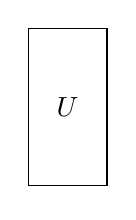
\begin{tikzpicture}[baseline=-0.5ex]
    \draw (0,0) rectangle (1,2) node[pos=.5] {$U$};
\end{tikzpicture}}}
\times 
\vcenter{\hbox{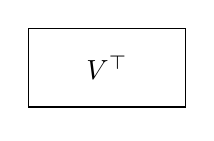
\begin{tikzpicture}[baseline=-0.5ex]
    \draw (0,0) rectangle (2,1) node[pos=.5] {$V^\top$};
\end{tikzpicture}}}
\,\right)
\]

\vspace{1em}
with state embeddings $U,V\in\R^{Z\times D}$
\vspace{1em}
\begin{itemize}
\item Can further parameterize $U$ or $V = \textrm{MLP}(E_u)$
\vspace{1em}
\item Similar for emissions
\end{itemize}
\end{frame}

\begin{frame}
\frametitle{Technique 2: State Dropout}
\begin{itemize}
\item Dropout is a common technique for regularizing neural networks \footcite{dropout}
\vspace{2em}
    \begin{itemize}
    \item Reduces a network's reliance on any particular neuron
        by via random masking
    \end{itemize}
\vspace{2em}
\item Extend dropout to the states of an HMM
\vspace{2em}
    \begin{itemize}
    \item Encourage broad utilization of all states
    \end{itemize}
\end{itemize}
\end{frame}

\begin{frame}
\frametitle{State Dropout}
\begin{itemize}
\item At each batch, sample dropout mask $\mathbf{b} \in \set{0,1}^{Z}$
\item Compute distributional parameters by indexing into embeddings $U,V$
\end{itemize}

\begin{center}
\begin{figure}
\begin{subfigure}{0.49\textwidth}
\centering
\[
\left(\,
\mathbf{b} \circ \vcenter{\hbox{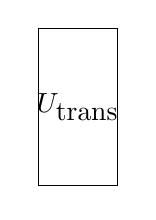
\begin{tikzpicture}[baseline=-0.5ex]
    \draw (0,0) rectangle (1,2) node[pos=.5] {$U_{\textnormal{trans}}$};
\end{tikzpicture}}}
\,\right)
\times
\left(\,
\mathbf{b} \circ
\vcenter{\hbox{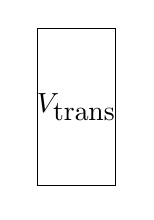
\begin{tikzpicture}[baseline=-0.5ex]
    \draw (0,0) rectangle (1,2) node[pos=.5] {$V_{\textnormal{trans}}$};
\end{tikzpicture}}}
\,\right)^\top
\]
\caption{Unnormalized transition logits}
\end{subfigure}
\begin{subfigure}{0.49\textwidth}
\centering
\[
\left(\,
\mathbf{b} \circ \vcenter{\hbox{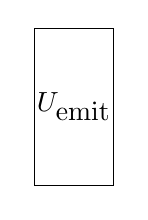
\begin{tikzpicture}[baseline=-0.5ex]
    \draw (0,0) rectangle (1,2) node[pos=.5] {$U_{\textnormal{emit}}$};
\end{tikzpicture}}}
\,\right)
\times
\vcenter{\hbox{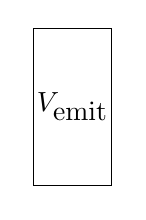
\begin{tikzpicture}[baseline=-0.5ex]
    \draw (0,0) rectangle (1,2) node[pos=.5] {$V_{\textnormal{emit}}$};
\end{tikzpicture}}}
^\top
\]
\caption{Unnormalized emission logits}
\end{subfigure}
\end{figure}
\end{center}
\end{frame}

\begin{frame}
\frametitle{State Dropout: Inference}
%The cost of inference is reduced by state dropout
\begin{center}
\resizebox{0.8\width}{0.8\height}{
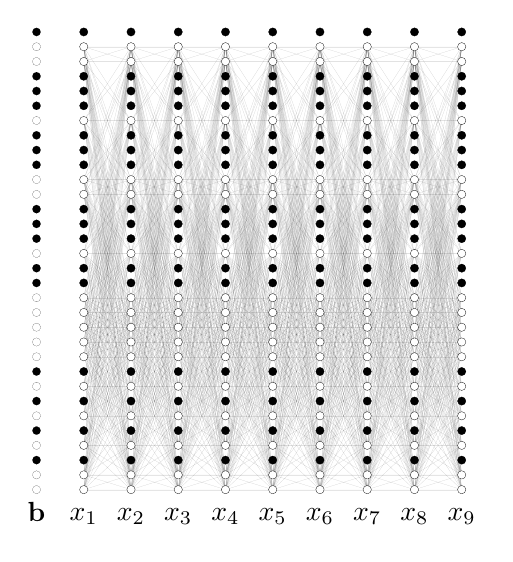
\begin{tikzpicture}%
\path[draw,line width=0.01pt,fill=white,radius=1.5pt] (0.0,0.0) circle;%
\path[draw,line width=0.01pt,fill=white,radius=1.5pt] (0.0,0.1875) circle;%
\path[draw,line width=0.01pt,fill=black,radius=1.5pt] (0.0,0.375) circle;%
\path[draw,line width=0.01pt,fill=white,radius=1.5pt] (0.0,0.5625) circle;%
\path[draw,line width=0.01pt,fill=black,radius=1.5pt] (0.0,0.75) circle;%
\path[draw,line width=0.01pt,fill=white,radius=1.5pt] (0.0,0.9375) circle;%
\path[draw,line width=0.01pt,fill=black,radius=1.5pt] (0.0,1.125) circle;%
\path[draw,line width=0.01pt,fill=white,radius=1.5pt] (0.0,1.3125) circle;%
\path[draw,line width=0.01pt,fill=black,radius=1.5pt] (0.0,1.5) circle;%
\path[draw,line width=0.01pt,fill=white,radius=1.5pt] (0.0,1.6875) circle;%
\path[draw,line width=0.01pt,fill=white,radius=1.5pt] (0.0,1.875) circle;%
\path[draw,line width=0.01pt,fill=white,radius=1.5pt] (0.0,2.0625) circle;%
\path[draw,line width=0.01pt,fill=white,radius=1.5pt] (0.0,2.25) circle;%
\path[draw,line width=0.01pt,fill=white,radius=1.5pt] (0.0,2.4375) circle;%
\path[draw,line width=0.01pt,fill=black,radius=1.5pt] (0.0,2.625) circle;%
\path[draw,line width=0.01pt,fill=black,radius=1.5pt] (0.0,2.8125) circle;%
\path[draw,line width=0.01pt,fill=white,radius=1.5pt] (0.0,3.0) circle;%
\path[draw,line width=0.01pt,fill=black,radius=1.5pt] (0.0,3.1875) circle;%
\path[draw,line width=0.01pt,fill=black,radius=1.5pt] (0.0,3.375) circle;%
\path[draw,line width=0.01pt,fill=black,radius=1.5pt] (0.0,3.5625) circle;%
\path[draw,line width=0.01pt,fill=white,radius=1.5pt] (0.0,3.75) circle;%
\path[draw,line width=0.01pt,fill=white,radius=1.5pt] (0.0,3.9375) circle;%
\path[draw,line width=0.01pt,fill=black,radius=1.5pt] (0.0,4.125) circle;%
\path[draw,line width=0.01pt,fill=black,radius=1.5pt] (0.0,4.3125) circle;%
\path[draw,line width=0.01pt,fill=black,radius=1.5pt] (0.0,4.5) circle;%
\path[draw,line width=0.01pt,fill=white,radius=1.5pt] (0.0,4.6875) circle;%
\path[draw,line width=0.01pt,fill=black,radius=1.5pt] (0.0,4.875) circle;%
\path[draw,line width=0.01pt,fill=black,radius=1.5pt] (0.0,5.0625) circle;%
\path[draw,line width=0.01pt,fill=black,radius=1.5pt] (0.0,5.25) circle;%
\path[draw,line width=0.01pt,fill=white,radius=1.5pt] (0.0,5.4375) circle;%
\path[draw,line width=0.01pt,fill=white,radius=1.5pt] (0.0,5.625) circle;%
\path[draw,line width=0.01pt,fill=black,radius=1.5pt] (0.0,5.8125) circle;%
\path[draw,line width=0.1pt,opacity=0.1,fill=black] (0.6,0.0) -- (1.2,0.0);%
\path[draw,line width=0.1pt,opacity=0.1,fill=black] (0.6,0.0) -- (1.2,0.1875);%
\path[draw,line width=0.1pt,opacity=0.1,fill=black] (0.6,0.0) -- (1.2,0.5625);%
\path[draw,line width=0.1pt,opacity=0.1,fill=black] (0.6,0.0) -- (1.2,0.9375);%
\path[draw,line width=0.1pt,opacity=0.1,fill=black] (0.6,0.0) -- (1.2,1.3125);%
\path[draw,line width=0.1pt,opacity=0.1,fill=black] (0.6,0.0) -- (1.2,1.6875);%
\path[draw,line width=0.1pt,opacity=0.1,fill=black] (0.6,0.0) -- (1.2,1.875);%
\path[draw,line width=0.1pt,opacity=0.1,fill=black] (0.6,0.0) -- (1.2,2.0625);%
\path[draw,line width=0.1pt,opacity=0.1,fill=black] (0.6,0.0) -- (1.2,2.25);%
\path[draw,line width=0.1pt,opacity=0.1,fill=black] (0.6,0.0) -- (1.2,2.4375);%
\path[draw,line width=0.1pt,opacity=0.1,fill=black] (0.6,0.0) -- (1.2,3.0);%
\path[draw,line width=0.1pt,opacity=0.1,fill=black] (0.6,0.0) -- (1.2,3.75);%
\path[draw,line width=0.1pt,opacity=0.1,fill=black] (0.6,0.0) -- (1.2,3.9375);%
\path[draw,line width=0.1pt,opacity=0.1,fill=black] (0.6,0.0) -- (1.2,4.6875);%
\path[draw,line width=0.1pt,opacity=0.1,fill=black] (0.6,0.0) -- (1.2,5.4375);%
\path[draw,line width=0.1pt,opacity=0.1,fill=black] (0.6,0.0) -- (1.2,5.625);%
\path[draw,line width=0.1pt,opacity=0.1,fill=black] (0.6,0.1875) -- (1.2,0.0);%
\path[draw,line width=0.1pt,opacity=0.1,fill=black] (0.6,0.1875) -- (1.2,0.1875);%
\path[draw,line width=0.1pt,opacity=0.1,fill=black] (0.6,0.1875) -- (1.2,0.5625);%
\path[draw,line width=0.1pt,opacity=0.1,fill=black] (0.6,0.1875) -- (1.2,0.9375);%
\path[draw,line width=0.1pt,opacity=0.1,fill=black] (0.6,0.1875) -- (1.2,1.3125);%
\path[draw,line width=0.1pt,opacity=0.1,fill=black] (0.6,0.1875) -- (1.2,1.6875);%
\path[draw,line width=0.1pt,opacity=0.1,fill=black] (0.6,0.1875) -- (1.2,1.875);%
\path[draw,line width=0.1pt,opacity=0.1,fill=black] (0.6,0.1875) -- (1.2,2.0625);%
\path[draw,line width=0.1pt,opacity=0.1,fill=black] (0.6,0.1875) -- (1.2,2.25);%
\path[draw,line width=0.1pt,opacity=0.1,fill=black] (0.6,0.1875) -- (1.2,2.4375);%
\path[draw,line width=0.1pt,opacity=0.1,fill=black] (0.6,0.1875) -- (1.2,3.0);%
\path[draw,line width=0.1pt,opacity=0.1,fill=black] (0.6,0.1875) -- (1.2,3.75);%
\path[draw,line width=0.1pt,opacity=0.1,fill=black] (0.6,0.1875) -- (1.2,3.9375);%
\path[draw,line width=0.1pt,opacity=0.1,fill=black] (0.6,0.1875) -- (1.2,4.6875);%
\path[draw,line width=0.1pt,opacity=0.1,fill=black] (0.6,0.1875) -- (1.2,5.4375);%
\path[draw,line width=0.1pt,opacity=0.1,fill=black] (0.6,0.1875) -- (1.2,5.625);%
\path[draw,line width=0.1pt,opacity=0.1,fill=black] (0.6,0.5625) -- (1.2,0.0);%
\path[draw,line width=0.1pt,opacity=0.1,fill=black] (0.6,0.5625) -- (1.2,0.1875);%
\path[draw,line width=0.1pt,opacity=0.1,fill=black] (0.6,0.5625) -- (1.2,0.5625);%
\path[draw,line width=0.1pt,opacity=0.1,fill=black] (0.6,0.5625) -- (1.2,0.9375);%
\path[draw,line width=0.1pt,opacity=0.1,fill=black] (0.6,0.5625) -- (1.2,1.3125);%
\path[draw,line width=0.1pt,opacity=0.1,fill=black] (0.6,0.5625) -- (1.2,1.6875);%
\path[draw,line width=0.1pt,opacity=0.1,fill=black] (0.6,0.5625) -- (1.2,1.875);%
\path[draw,line width=0.1pt,opacity=0.1,fill=black] (0.6,0.5625) -- (1.2,2.0625);%
\path[draw,line width=0.1pt,opacity=0.1,fill=black] (0.6,0.5625) -- (1.2,2.25);%
\path[draw,line width=0.1pt,opacity=0.1,fill=black] (0.6,0.5625) -- (1.2,2.4375);%
\path[draw,line width=0.1pt,opacity=0.1,fill=black] (0.6,0.5625) -- (1.2,3.0);%
\path[draw,line width=0.1pt,opacity=0.1,fill=black] (0.6,0.5625) -- (1.2,3.75);%
\path[draw,line width=0.1pt,opacity=0.1,fill=black] (0.6,0.5625) -- (1.2,3.9375);%
\path[draw,line width=0.1pt,opacity=0.1,fill=black] (0.6,0.5625) -- (1.2,4.6875);%
\path[draw,line width=0.1pt,opacity=0.1,fill=black] (0.6,0.5625) -- (1.2,5.4375);%
\path[draw,line width=0.1pt,opacity=0.1,fill=black] (0.6,0.5625) -- (1.2,5.625);%
\path[draw,line width=0.1pt,opacity=0.1,fill=black] (0.6,0.9375) -- (1.2,0.0);%
\path[draw,line width=0.1pt,opacity=0.1,fill=black] (0.6,0.9375) -- (1.2,0.1875);%
\path[draw,line width=0.1pt,opacity=0.1,fill=black] (0.6,0.9375) -- (1.2,0.5625);%
\path[draw,line width=0.1pt,opacity=0.1,fill=black] (0.6,0.9375) -- (1.2,0.9375);%
\path[draw,line width=0.1pt,opacity=0.1,fill=black] (0.6,0.9375) -- (1.2,1.3125);%
\path[draw,line width=0.1pt,opacity=0.1,fill=black] (0.6,0.9375) -- (1.2,1.6875);%
\path[draw,line width=0.1pt,opacity=0.1,fill=black] (0.6,0.9375) -- (1.2,1.875);%
\path[draw,line width=0.1pt,opacity=0.1,fill=black] (0.6,0.9375) -- (1.2,2.0625);%
\path[draw,line width=0.1pt,opacity=0.1,fill=black] (0.6,0.9375) -- (1.2,2.25);%
\path[draw,line width=0.1pt,opacity=0.1,fill=black] (0.6,0.9375) -- (1.2,2.4375);%
\path[draw,line width=0.1pt,opacity=0.1,fill=black] (0.6,0.9375) -- (1.2,3.0);%
\path[draw,line width=0.1pt,opacity=0.1,fill=black] (0.6,0.9375) -- (1.2,3.75);%
\path[draw,line width=0.1pt,opacity=0.1,fill=black] (0.6,0.9375) -- (1.2,3.9375);%
\path[draw,line width=0.1pt,opacity=0.1,fill=black] (0.6,0.9375) -- (1.2,4.6875);%
\path[draw,line width=0.1pt,opacity=0.1,fill=black] (0.6,0.9375) -- (1.2,5.4375);%
\path[draw,line width=0.1pt,opacity=0.1,fill=black] (0.6,0.9375) -- (1.2,5.625);%
\path[draw,line width=0.1pt,opacity=0.1,fill=black] (0.6,1.3125) -- (1.2,0.0);%
\path[draw,line width=0.1pt,opacity=0.1,fill=black] (0.6,1.3125) -- (1.2,0.1875);%
\path[draw,line width=0.1pt,opacity=0.1,fill=black] (0.6,1.3125) -- (1.2,0.5625);%
\path[draw,line width=0.1pt,opacity=0.1,fill=black] (0.6,1.3125) -- (1.2,0.9375);%
\path[draw,line width=0.1pt,opacity=0.1,fill=black] (0.6,1.3125) -- (1.2,1.3125);%
\path[draw,line width=0.1pt,opacity=0.1,fill=black] (0.6,1.3125) -- (1.2,1.6875);%
\path[draw,line width=0.1pt,opacity=0.1,fill=black] (0.6,1.3125) -- (1.2,1.875);%
\path[draw,line width=0.1pt,opacity=0.1,fill=black] (0.6,1.3125) -- (1.2,2.0625);%
\path[draw,line width=0.1pt,opacity=0.1,fill=black] (0.6,1.3125) -- (1.2,2.25);%
\path[draw,line width=0.1pt,opacity=0.1,fill=black] (0.6,1.3125) -- (1.2,2.4375);%
\path[draw,line width=0.1pt,opacity=0.1,fill=black] (0.6,1.3125) -- (1.2,3.0);%
\path[draw,line width=0.1pt,opacity=0.1,fill=black] (0.6,1.3125) -- (1.2,3.75);%
\path[draw,line width=0.1pt,opacity=0.1,fill=black] (0.6,1.3125) -- (1.2,3.9375);%
\path[draw,line width=0.1pt,opacity=0.1,fill=black] (0.6,1.3125) -- (1.2,4.6875);%
\path[draw,line width=0.1pt,opacity=0.1,fill=black] (0.6,1.3125) -- (1.2,5.4375);%
\path[draw,line width=0.1pt,opacity=0.1,fill=black] (0.6,1.3125) -- (1.2,5.625);%
\path[draw,line width=0.1pt,opacity=0.1,fill=black] (0.6,1.6875) -- (1.2,0.0);%
\path[draw,line width=0.1pt,opacity=0.1,fill=black] (0.6,1.6875) -- (1.2,0.1875);%
\path[draw,line width=0.1pt,opacity=0.1,fill=black] (0.6,1.6875) -- (1.2,0.5625);%
\path[draw,line width=0.1pt,opacity=0.1,fill=black] (0.6,1.6875) -- (1.2,0.9375);%
\path[draw,line width=0.1pt,opacity=0.1,fill=black] (0.6,1.6875) -- (1.2,1.3125);%
\path[draw,line width=0.1pt,opacity=0.1,fill=black] (0.6,1.6875) -- (1.2,1.6875);%
\path[draw,line width=0.1pt,opacity=0.1,fill=black] (0.6,1.6875) -- (1.2,1.875);%
\path[draw,line width=0.1pt,opacity=0.1,fill=black] (0.6,1.6875) -- (1.2,2.0625);%
\path[draw,line width=0.1pt,opacity=0.1,fill=black] (0.6,1.6875) -- (1.2,2.25);%
\path[draw,line width=0.1pt,opacity=0.1,fill=black] (0.6,1.6875) -- (1.2,2.4375);%
\path[draw,line width=0.1pt,opacity=0.1,fill=black] (0.6,1.6875) -- (1.2,3.0);%
\path[draw,line width=0.1pt,opacity=0.1,fill=black] (0.6,1.6875) -- (1.2,3.75);%
\path[draw,line width=0.1pt,opacity=0.1,fill=black] (0.6,1.6875) -- (1.2,3.9375);%
\path[draw,line width=0.1pt,opacity=0.1,fill=black] (0.6,1.6875) -- (1.2,4.6875);%
\path[draw,line width=0.1pt,opacity=0.1,fill=black] (0.6,1.6875) -- (1.2,5.4375);%
\path[draw,line width=0.1pt,opacity=0.1,fill=black] (0.6,1.6875) -- (1.2,5.625);%
\path[draw,line width=0.1pt,opacity=0.1,fill=black] (0.6,1.875) -- (1.2,0.0);%
\path[draw,line width=0.1pt,opacity=0.1,fill=black] (0.6,1.875) -- (1.2,0.1875);%
\path[draw,line width=0.1pt,opacity=0.1,fill=black] (0.6,1.875) -- (1.2,0.5625);%
\path[draw,line width=0.1pt,opacity=0.1,fill=black] (0.6,1.875) -- (1.2,0.9375);%
\path[draw,line width=0.1pt,opacity=0.1,fill=black] (0.6,1.875) -- (1.2,1.3125);%
\path[draw,line width=0.1pt,opacity=0.1,fill=black] (0.6,1.875) -- (1.2,1.6875);%
\path[draw,line width=0.1pt,opacity=0.1,fill=black] (0.6,1.875) -- (1.2,1.875);%
\path[draw,line width=0.1pt,opacity=0.1,fill=black] (0.6,1.875) -- (1.2,2.0625);%
\path[draw,line width=0.1pt,opacity=0.1,fill=black] (0.6,1.875) -- (1.2,2.25);%
\path[draw,line width=0.1pt,opacity=0.1,fill=black] (0.6,1.875) -- (1.2,2.4375);%
\path[draw,line width=0.1pt,opacity=0.1,fill=black] (0.6,1.875) -- (1.2,3.0);%
\path[draw,line width=0.1pt,opacity=0.1,fill=black] (0.6,1.875) -- (1.2,3.75);%
\path[draw,line width=0.1pt,opacity=0.1,fill=black] (0.6,1.875) -- (1.2,3.9375);%
\path[draw,line width=0.1pt,opacity=0.1,fill=black] (0.6,1.875) -- (1.2,4.6875);%
\path[draw,line width=0.1pt,opacity=0.1,fill=black] (0.6,1.875) -- (1.2,5.4375);%
\path[draw,line width=0.1pt,opacity=0.1,fill=black] (0.6,1.875) -- (1.2,5.625);%
\path[draw,line width=0.1pt,opacity=0.1,fill=black] (0.6,2.0625) -- (1.2,0.0);%
\path[draw,line width=0.1pt,opacity=0.1,fill=black] (0.6,2.0625) -- (1.2,0.1875);%
\path[draw,line width=0.1pt,opacity=0.1,fill=black] (0.6,2.0625) -- (1.2,0.5625);%
\path[draw,line width=0.1pt,opacity=0.1,fill=black] (0.6,2.0625) -- (1.2,0.9375);%
\path[draw,line width=0.1pt,opacity=0.1,fill=black] (0.6,2.0625) -- (1.2,1.3125);%
\path[draw,line width=0.1pt,opacity=0.1,fill=black] (0.6,2.0625) -- (1.2,1.6875);%
\path[draw,line width=0.1pt,opacity=0.1,fill=black] (0.6,2.0625) -- (1.2,1.875);%
\path[draw,line width=0.1pt,opacity=0.1,fill=black] (0.6,2.0625) -- (1.2,2.0625);%
\path[draw,line width=0.1pt,opacity=0.1,fill=black] (0.6,2.0625) -- (1.2,2.25);%
\path[draw,line width=0.1pt,opacity=0.1,fill=black] (0.6,2.0625) -- (1.2,2.4375);%
\path[draw,line width=0.1pt,opacity=0.1,fill=black] (0.6,2.0625) -- (1.2,3.0);%
\path[draw,line width=0.1pt,opacity=0.1,fill=black] (0.6,2.0625) -- (1.2,3.75);%
\path[draw,line width=0.1pt,opacity=0.1,fill=black] (0.6,2.0625) -- (1.2,3.9375);%
\path[draw,line width=0.1pt,opacity=0.1,fill=black] (0.6,2.0625) -- (1.2,4.6875);%
\path[draw,line width=0.1pt,opacity=0.1,fill=black] (0.6,2.0625) -- (1.2,5.4375);%
\path[draw,line width=0.1pt,opacity=0.1,fill=black] (0.6,2.0625) -- (1.2,5.625);%
\path[draw,line width=0.1pt,opacity=0.1,fill=black] (0.6,2.25) -- (1.2,0.0);%
\path[draw,line width=0.1pt,opacity=0.1,fill=black] (0.6,2.25) -- (1.2,0.1875);%
\path[draw,line width=0.1pt,opacity=0.1,fill=black] (0.6,2.25) -- (1.2,0.5625);%
\path[draw,line width=0.1pt,opacity=0.1,fill=black] (0.6,2.25) -- (1.2,0.9375);%
\path[draw,line width=0.1pt,opacity=0.1,fill=black] (0.6,2.25) -- (1.2,1.3125);%
\path[draw,line width=0.1pt,opacity=0.1,fill=black] (0.6,2.25) -- (1.2,1.6875);%
\path[draw,line width=0.1pt,opacity=0.1,fill=black] (0.6,2.25) -- (1.2,1.875);%
\path[draw,line width=0.1pt,opacity=0.1,fill=black] (0.6,2.25) -- (1.2,2.0625);%
\path[draw,line width=0.1pt,opacity=0.1,fill=black] (0.6,2.25) -- (1.2,2.25);%
\path[draw,line width=0.1pt,opacity=0.1,fill=black] (0.6,2.25) -- (1.2,2.4375);%
\path[draw,line width=0.1pt,opacity=0.1,fill=black] (0.6,2.25) -- (1.2,3.0);%
\path[draw,line width=0.1pt,opacity=0.1,fill=black] (0.6,2.25) -- (1.2,3.75);%
\path[draw,line width=0.1pt,opacity=0.1,fill=black] (0.6,2.25) -- (1.2,3.9375);%
\path[draw,line width=0.1pt,opacity=0.1,fill=black] (0.6,2.25) -- (1.2,4.6875);%
\path[draw,line width=0.1pt,opacity=0.1,fill=black] (0.6,2.25) -- (1.2,5.4375);%
\path[draw,line width=0.1pt,opacity=0.1,fill=black] (0.6,2.25) -- (1.2,5.625);%
\path[draw,line width=0.1pt,opacity=0.1,fill=black] (0.6,2.4375) -- (1.2,0.0);%
\path[draw,line width=0.1pt,opacity=0.1,fill=black] (0.6,2.4375) -- (1.2,0.1875);%
\path[draw,line width=0.1pt,opacity=0.1,fill=black] (0.6,2.4375) -- (1.2,0.5625);%
\path[draw,line width=0.1pt,opacity=0.1,fill=black] (0.6,2.4375) -- (1.2,0.9375);%
\path[draw,line width=0.1pt,opacity=0.1,fill=black] (0.6,2.4375) -- (1.2,1.3125);%
\path[draw,line width=0.1pt,opacity=0.1,fill=black] (0.6,2.4375) -- (1.2,1.6875);%
\path[draw,line width=0.1pt,opacity=0.1,fill=black] (0.6,2.4375) -- (1.2,1.875);%
\path[draw,line width=0.1pt,opacity=0.1,fill=black] (0.6,2.4375) -- (1.2,2.0625);%
\path[draw,line width=0.1pt,opacity=0.1,fill=black] (0.6,2.4375) -- (1.2,2.25);%
\path[draw,line width=0.1pt,opacity=0.1,fill=black] (0.6,2.4375) -- (1.2,2.4375);%
\path[draw,line width=0.1pt,opacity=0.1,fill=black] (0.6,2.4375) -- (1.2,3.0);%
\path[draw,line width=0.1pt,opacity=0.1,fill=black] (0.6,2.4375) -- (1.2,3.75);%
\path[draw,line width=0.1pt,opacity=0.1,fill=black] (0.6,2.4375) -- (1.2,3.9375);%
\path[draw,line width=0.1pt,opacity=0.1,fill=black] (0.6,2.4375) -- (1.2,4.6875);%
\path[draw,line width=0.1pt,opacity=0.1,fill=black] (0.6,2.4375) -- (1.2,5.4375);%
\path[draw,line width=0.1pt,opacity=0.1,fill=black] (0.6,2.4375) -- (1.2,5.625);%
\path[draw,line width=0.1pt,opacity=0.1,fill=black] (0.6,3.0) -- (1.2,0.0);%
\path[draw,line width=0.1pt,opacity=0.1,fill=black] (0.6,3.0) -- (1.2,0.1875);%
\path[draw,line width=0.1pt,opacity=0.1,fill=black] (0.6,3.0) -- (1.2,0.5625);%
\path[draw,line width=0.1pt,opacity=0.1,fill=black] (0.6,3.0) -- (1.2,0.9375);%
\path[draw,line width=0.1pt,opacity=0.1,fill=black] (0.6,3.0) -- (1.2,1.3125);%
\path[draw,line width=0.1pt,opacity=0.1,fill=black] (0.6,3.0) -- (1.2,1.6875);%
\path[draw,line width=0.1pt,opacity=0.1,fill=black] (0.6,3.0) -- (1.2,1.875);%
\path[draw,line width=0.1pt,opacity=0.1,fill=black] (0.6,3.0) -- (1.2,2.0625);%
\path[draw,line width=0.1pt,opacity=0.1,fill=black] (0.6,3.0) -- (1.2,2.25);%
\path[draw,line width=0.1pt,opacity=0.1,fill=black] (0.6,3.0) -- (1.2,2.4375);%
\path[draw,line width=0.1pt,opacity=0.1,fill=black] (0.6,3.0) -- (1.2,3.0);%
\path[draw,line width=0.1pt,opacity=0.1,fill=black] (0.6,3.0) -- (1.2,3.75);%
\path[draw,line width=0.1pt,opacity=0.1,fill=black] (0.6,3.0) -- (1.2,3.9375);%
\path[draw,line width=0.1pt,opacity=0.1,fill=black] (0.6,3.0) -- (1.2,4.6875);%
\path[draw,line width=0.1pt,opacity=0.1,fill=black] (0.6,3.0) -- (1.2,5.4375);%
\path[draw,line width=0.1pt,opacity=0.1,fill=black] (0.6,3.0) -- (1.2,5.625);%
\path[draw,line width=0.1pt,opacity=0.1,fill=black] (0.6,3.75) -- (1.2,0.0);%
\path[draw,line width=0.1pt,opacity=0.1,fill=black] (0.6,3.75) -- (1.2,0.1875);%
\path[draw,line width=0.1pt,opacity=0.1,fill=black] (0.6,3.75) -- (1.2,0.5625);%
\path[draw,line width=0.1pt,opacity=0.1,fill=black] (0.6,3.75) -- (1.2,0.9375);%
\path[draw,line width=0.1pt,opacity=0.1,fill=black] (0.6,3.75) -- (1.2,1.3125);%
\path[draw,line width=0.1pt,opacity=0.1,fill=black] (0.6,3.75) -- (1.2,1.6875);%
\path[draw,line width=0.1pt,opacity=0.1,fill=black] (0.6,3.75) -- (1.2,1.875);%
\path[draw,line width=0.1pt,opacity=0.1,fill=black] (0.6,3.75) -- (1.2,2.0625);%
\path[draw,line width=0.1pt,opacity=0.1,fill=black] (0.6,3.75) -- (1.2,2.25);%
\path[draw,line width=0.1pt,opacity=0.1,fill=black] (0.6,3.75) -- (1.2,2.4375);%
\path[draw,line width=0.1pt,opacity=0.1,fill=black] (0.6,3.75) -- (1.2,3.0);%
\path[draw,line width=0.1pt,opacity=0.1,fill=black] (0.6,3.75) -- (1.2,3.75);%
\path[draw,line width=0.1pt,opacity=0.1,fill=black] (0.6,3.75) -- (1.2,3.9375);%
\path[draw,line width=0.1pt,opacity=0.1,fill=black] (0.6,3.75) -- (1.2,4.6875);%
\path[draw,line width=0.1pt,opacity=0.1,fill=black] (0.6,3.75) -- (1.2,5.4375);%
\path[draw,line width=0.1pt,opacity=0.1,fill=black] (0.6,3.75) -- (1.2,5.625);%
\path[draw,line width=0.1pt,opacity=0.1,fill=black] (0.6,3.9375) -- (1.2,0.0);%
\path[draw,line width=0.1pt,opacity=0.1,fill=black] (0.6,3.9375) -- (1.2,0.1875);%
\path[draw,line width=0.1pt,opacity=0.1,fill=black] (0.6,3.9375) -- (1.2,0.5625);%
\path[draw,line width=0.1pt,opacity=0.1,fill=black] (0.6,3.9375) -- (1.2,0.9375);%
\path[draw,line width=0.1pt,opacity=0.1,fill=black] (0.6,3.9375) -- (1.2,1.3125);%
\path[draw,line width=0.1pt,opacity=0.1,fill=black] (0.6,3.9375) -- (1.2,1.6875);%
\path[draw,line width=0.1pt,opacity=0.1,fill=black] (0.6,3.9375) -- (1.2,1.875);%
\path[draw,line width=0.1pt,opacity=0.1,fill=black] (0.6,3.9375) -- (1.2,2.0625);%
\path[draw,line width=0.1pt,opacity=0.1,fill=black] (0.6,3.9375) -- (1.2,2.25);%
\path[draw,line width=0.1pt,opacity=0.1,fill=black] (0.6,3.9375) -- (1.2,2.4375);%
\path[draw,line width=0.1pt,opacity=0.1,fill=black] (0.6,3.9375) -- (1.2,3.0);%
\path[draw,line width=0.1pt,opacity=0.1,fill=black] (0.6,3.9375) -- (1.2,3.75);%
\path[draw,line width=0.1pt,opacity=0.1,fill=black] (0.6,3.9375) -- (1.2,3.9375);%
\path[draw,line width=0.1pt,opacity=0.1,fill=black] (0.6,3.9375) -- (1.2,4.6875);%
\path[draw,line width=0.1pt,opacity=0.1,fill=black] (0.6,3.9375) -- (1.2,5.4375);%
\path[draw,line width=0.1pt,opacity=0.1,fill=black] (0.6,3.9375) -- (1.2,5.625);%
\path[draw,line width=0.1pt,opacity=0.1,fill=black] (0.6,4.6875) -- (1.2,0.0);%
\path[draw,line width=0.1pt,opacity=0.1,fill=black] (0.6,4.6875) -- (1.2,0.1875);%
\path[draw,line width=0.1pt,opacity=0.1,fill=black] (0.6,4.6875) -- (1.2,0.5625);%
\path[draw,line width=0.1pt,opacity=0.1,fill=black] (0.6,4.6875) -- (1.2,0.9375);%
\path[draw,line width=0.1pt,opacity=0.1,fill=black] (0.6,4.6875) -- (1.2,1.3125);%
\path[draw,line width=0.1pt,opacity=0.1,fill=black] (0.6,4.6875) -- (1.2,1.6875);%
\path[draw,line width=0.1pt,opacity=0.1,fill=black] (0.6,4.6875) -- (1.2,1.875);%
\path[draw,line width=0.1pt,opacity=0.1,fill=black] (0.6,4.6875) -- (1.2,2.0625);%
\path[draw,line width=0.1pt,opacity=0.1,fill=black] (0.6,4.6875) -- (1.2,2.25);%
\path[draw,line width=0.1pt,opacity=0.1,fill=black] (0.6,4.6875) -- (1.2,2.4375);%
\path[draw,line width=0.1pt,opacity=0.1,fill=black] (0.6,4.6875) -- (1.2,3.0);%
\path[draw,line width=0.1pt,opacity=0.1,fill=black] (0.6,4.6875) -- (1.2,3.75);%
\path[draw,line width=0.1pt,opacity=0.1,fill=black] (0.6,4.6875) -- (1.2,3.9375);%
\path[draw,line width=0.1pt,opacity=0.1,fill=black] (0.6,4.6875) -- (1.2,4.6875);%
\path[draw,line width=0.1pt,opacity=0.1,fill=black] (0.6,4.6875) -- (1.2,5.4375);%
\path[draw,line width=0.1pt,opacity=0.1,fill=black] (0.6,4.6875) -- (1.2,5.625);%
\path[draw,line width=0.1pt,opacity=0.1,fill=black] (0.6,5.4375) -- (1.2,0.0);%
\path[draw,line width=0.1pt,opacity=0.1,fill=black] (0.6,5.4375) -- (1.2,0.1875);%
\path[draw,line width=0.1pt,opacity=0.1,fill=black] (0.6,5.4375) -- (1.2,0.5625);%
\path[draw,line width=0.1pt,opacity=0.1,fill=black] (0.6,5.4375) -- (1.2,0.9375);%
\path[draw,line width=0.1pt,opacity=0.1,fill=black] (0.6,5.4375) -- (1.2,1.3125);%
\path[draw,line width=0.1pt,opacity=0.1,fill=black] (0.6,5.4375) -- (1.2,1.6875);%
\path[draw,line width=0.1pt,opacity=0.1,fill=black] (0.6,5.4375) -- (1.2,1.875);%
\path[draw,line width=0.1pt,opacity=0.1,fill=black] (0.6,5.4375) -- (1.2,2.0625);%
\path[draw,line width=0.1pt,opacity=0.1,fill=black] (0.6,5.4375) -- (1.2,2.25);%
\path[draw,line width=0.1pt,opacity=0.1,fill=black] (0.6,5.4375) -- (1.2,2.4375);%
\path[draw,line width=0.1pt,opacity=0.1,fill=black] (0.6,5.4375) -- (1.2,3.0);%
\path[draw,line width=0.1pt,opacity=0.1,fill=black] (0.6,5.4375) -- (1.2,3.75);%
\path[draw,line width=0.1pt,opacity=0.1,fill=black] (0.6,5.4375) -- (1.2,3.9375);%
\path[draw,line width=0.1pt,opacity=0.1,fill=black] (0.6,5.4375) -- (1.2,4.6875);%
\path[draw,line width=0.1pt,opacity=0.1,fill=black] (0.6,5.4375) -- (1.2,5.4375);%
\path[draw,line width=0.1pt,opacity=0.1,fill=black] (0.6,5.4375) -- (1.2,5.625);%
\path[draw,line width=0.1pt,opacity=0.1,fill=black] (0.6,5.625) -- (1.2,0.0);%
\path[draw,line width=0.1pt,opacity=0.1,fill=black] (0.6,5.625) -- (1.2,0.1875);%
\path[draw,line width=0.1pt,opacity=0.1,fill=black] (0.6,5.625) -- (1.2,0.5625);%
\path[draw,line width=0.1pt,opacity=0.1,fill=black] (0.6,5.625) -- (1.2,0.9375);%
\path[draw,line width=0.1pt,opacity=0.1,fill=black] (0.6,5.625) -- (1.2,1.3125);%
\path[draw,line width=0.1pt,opacity=0.1,fill=black] (0.6,5.625) -- (1.2,1.6875);%
\path[draw,line width=0.1pt,opacity=0.1,fill=black] (0.6,5.625) -- (1.2,1.875);%
\path[draw,line width=0.1pt,opacity=0.1,fill=black] (0.6,5.625) -- (1.2,2.0625);%
\path[draw,line width=0.1pt,opacity=0.1,fill=black] (0.6,5.625) -- (1.2,2.25);%
\path[draw,line width=0.1pt,opacity=0.1,fill=black] (0.6,5.625) -- (1.2,2.4375);%
\path[draw,line width=0.1pt,opacity=0.1,fill=black] (0.6,5.625) -- (1.2,3.0);%
\path[draw,line width=0.1pt,opacity=0.1,fill=black] (0.6,5.625) -- (1.2,3.75);%
\path[draw,line width=0.1pt,opacity=0.1,fill=black] (0.6,5.625) -- (1.2,3.9375);%
\path[draw,line width=0.1pt,opacity=0.1,fill=black] (0.6,5.625) -- (1.2,4.6875);%
\path[draw,line width=0.1pt,opacity=0.1,fill=black] (0.6,5.625) -- (1.2,5.4375);%
\path[draw,line width=0.1pt,opacity=0.1,fill=black] (0.6,5.625) -- (1.2,5.625);%
\path[draw,line width=0.1pt,opacity=0.1,fill=black] (1.2,0.0) -- (1.8,0.0);%
\path[draw,line width=0.1pt,opacity=0.1,fill=black] (1.2,0.0) -- (1.8,0.1875);%
\path[draw,line width=0.1pt,opacity=0.1,fill=black] (1.2,0.0) -- (1.8,0.5625);%
\path[draw,line width=0.1pt,opacity=0.1,fill=black] (1.2,0.0) -- (1.8,0.9375);%
\path[draw,line width=0.1pt,opacity=0.1,fill=black] (1.2,0.0) -- (1.8,1.3125);%
\path[draw,line width=0.1pt,opacity=0.1,fill=black] (1.2,0.0) -- (1.8,1.6875);%
\path[draw,line width=0.1pt,opacity=0.1,fill=black] (1.2,0.0) -- (1.8,1.875);%
\path[draw,line width=0.1pt,opacity=0.1,fill=black] (1.2,0.0) -- (1.8,2.0625);%
\path[draw,line width=0.1pt,opacity=0.1,fill=black] (1.2,0.0) -- (1.8,2.25);%
\path[draw,line width=0.1pt,opacity=0.1,fill=black] (1.2,0.0) -- (1.8,2.4375);%
\path[draw,line width=0.1pt,opacity=0.1,fill=black] (1.2,0.0) -- (1.8,3.0);%
\path[draw,line width=0.1pt,opacity=0.1,fill=black] (1.2,0.0) -- (1.8,3.75);%
\path[draw,line width=0.1pt,opacity=0.1,fill=black] (1.2,0.0) -- (1.8,3.9375);%
\path[draw,line width=0.1pt,opacity=0.1,fill=black] (1.2,0.0) -- (1.8,4.6875);%
\path[draw,line width=0.1pt,opacity=0.1,fill=black] (1.2,0.0) -- (1.8,5.4375);%
\path[draw,line width=0.1pt,opacity=0.1,fill=black] (1.2,0.0) -- (1.8,5.625);%
\path[draw,line width=0.1pt,opacity=0.1,fill=black] (1.2,0.1875) -- (1.8,0.0);%
\path[draw,line width=0.1pt,opacity=0.1,fill=black] (1.2,0.1875) -- (1.8,0.1875);%
\path[draw,line width=0.1pt,opacity=0.1,fill=black] (1.2,0.1875) -- (1.8,0.5625);%
\path[draw,line width=0.1pt,opacity=0.1,fill=black] (1.2,0.1875) -- (1.8,0.9375);%
\path[draw,line width=0.1pt,opacity=0.1,fill=black] (1.2,0.1875) -- (1.8,1.3125);%
\path[draw,line width=0.1pt,opacity=0.1,fill=black] (1.2,0.1875) -- (1.8,1.6875);%
\path[draw,line width=0.1pt,opacity=0.1,fill=black] (1.2,0.1875) -- (1.8,1.875);%
\path[draw,line width=0.1pt,opacity=0.1,fill=black] (1.2,0.1875) -- (1.8,2.0625);%
\path[draw,line width=0.1pt,opacity=0.1,fill=black] (1.2,0.1875) -- (1.8,2.25);%
\path[draw,line width=0.1pt,opacity=0.1,fill=black] (1.2,0.1875) -- (1.8,2.4375);%
\path[draw,line width=0.1pt,opacity=0.1,fill=black] (1.2,0.1875) -- (1.8,3.0);%
\path[draw,line width=0.1pt,opacity=0.1,fill=black] (1.2,0.1875) -- (1.8,3.75);%
\path[draw,line width=0.1pt,opacity=0.1,fill=black] (1.2,0.1875) -- (1.8,3.9375);%
\path[draw,line width=0.1pt,opacity=0.1,fill=black] (1.2,0.1875) -- (1.8,4.6875);%
\path[draw,line width=0.1pt,opacity=0.1,fill=black] (1.2,0.1875) -- (1.8,5.4375);%
\path[draw,line width=0.1pt,opacity=0.1,fill=black] (1.2,0.1875) -- (1.8,5.625);%
\path[draw,line width=0.1pt,opacity=0.1,fill=black] (1.2,0.5625) -- (1.8,0.0);%
\path[draw,line width=0.1pt,opacity=0.1,fill=black] (1.2,0.5625) -- (1.8,0.1875);%
\path[draw,line width=0.1pt,opacity=0.1,fill=black] (1.2,0.5625) -- (1.8,0.5625);%
\path[draw,line width=0.1pt,opacity=0.1,fill=black] (1.2,0.5625) -- (1.8,0.9375);%
\path[draw,line width=0.1pt,opacity=0.1,fill=black] (1.2,0.5625) -- (1.8,1.3125);%
\path[draw,line width=0.1pt,opacity=0.1,fill=black] (1.2,0.5625) -- (1.8,1.6875);%
\path[draw,line width=0.1pt,opacity=0.1,fill=black] (1.2,0.5625) -- (1.8,1.875);%
\path[draw,line width=0.1pt,opacity=0.1,fill=black] (1.2,0.5625) -- (1.8,2.0625);%
\path[draw,line width=0.1pt,opacity=0.1,fill=black] (1.2,0.5625) -- (1.8,2.25);%
\path[draw,line width=0.1pt,opacity=0.1,fill=black] (1.2,0.5625) -- (1.8,2.4375);%
\path[draw,line width=0.1pt,opacity=0.1,fill=black] (1.2,0.5625) -- (1.8,3.0);%
\path[draw,line width=0.1pt,opacity=0.1,fill=black] (1.2,0.5625) -- (1.8,3.75);%
\path[draw,line width=0.1pt,opacity=0.1,fill=black] (1.2,0.5625) -- (1.8,3.9375);%
\path[draw,line width=0.1pt,opacity=0.1,fill=black] (1.2,0.5625) -- (1.8,4.6875);%
\path[draw,line width=0.1pt,opacity=0.1,fill=black] (1.2,0.5625) -- (1.8,5.4375);%
\path[draw,line width=0.1pt,opacity=0.1,fill=black] (1.2,0.5625) -- (1.8,5.625);%
\path[draw,line width=0.1pt,opacity=0.1,fill=black] (1.2,0.9375) -- (1.8,0.0);%
\path[draw,line width=0.1pt,opacity=0.1,fill=black] (1.2,0.9375) -- (1.8,0.1875);%
\path[draw,line width=0.1pt,opacity=0.1,fill=black] (1.2,0.9375) -- (1.8,0.5625);%
\path[draw,line width=0.1pt,opacity=0.1,fill=black] (1.2,0.9375) -- (1.8,0.9375);%
\path[draw,line width=0.1pt,opacity=0.1,fill=black] (1.2,0.9375) -- (1.8,1.3125);%
\path[draw,line width=0.1pt,opacity=0.1,fill=black] (1.2,0.9375) -- (1.8,1.6875);%
\path[draw,line width=0.1pt,opacity=0.1,fill=black] (1.2,0.9375) -- (1.8,1.875);%
\path[draw,line width=0.1pt,opacity=0.1,fill=black] (1.2,0.9375) -- (1.8,2.0625);%
\path[draw,line width=0.1pt,opacity=0.1,fill=black] (1.2,0.9375) -- (1.8,2.25);%
\path[draw,line width=0.1pt,opacity=0.1,fill=black] (1.2,0.9375) -- (1.8,2.4375);%
\path[draw,line width=0.1pt,opacity=0.1,fill=black] (1.2,0.9375) -- (1.8,3.0);%
\path[draw,line width=0.1pt,opacity=0.1,fill=black] (1.2,0.9375) -- (1.8,3.75);%
\path[draw,line width=0.1pt,opacity=0.1,fill=black] (1.2,0.9375) -- (1.8,3.9375);%
\path[draw,line width=0.1pt,opacity=0.1,fill=black] (1.2,0.9375) -- (1.8,4.6875);%
\path[draw,line width=0.1pt,opacity=0.1,fill=black] (1.2,0.9375) -- (1.8,5.4375);%
\path[draw,line width=0.1pt,opacity=0.1,fill=black] (1.2,0.9375) -- (1.8,5.625);%
\path[draw,line width=0.1pt,opacity=0.1,fill=black] (1.2,1.3125) -- (1.8,0.0);%
\path[draw,line width=0.1pt,opacity=0.1,fill=black] (1.2,1.3125) -- (1.8,0.1875);%
\path[draw,line width=0.1pt,opacity=0.1,fill=black] (1.2,1.3125) -- (1.8,0.5625);%
\path[draw,line width=0.1pt,opacity=0.1,fill=black] (1.2,1.3125) -- (1.8,0.9375);%
\path[draw,line width=0.1pt,opacity=0.1,fill=black] (1.2,1.3125) -- (1.8,1.3125);%
\path[draw,line width=0.1pt,opacity=0.1,fill=black] (1.2,1.3125) -- (1.8,1.6875);%
\path[draw,line width=0.1pt,opacity=0.1,fill=black] (1.2,1.3125) -- (1.8,1.875);%
\path[draw,line width=0.1pt,opacity=0.1,fill=black] (1.2,1.3125) -- (1.8,2.0625);%
\path[draw,line width=0.1pt,opacity=0.1,fill=black] (1.2,1.3125) -- (1.8,2.25);%
\path[draw,line width=0.1pt,opacity=0.1,fill=black] (1.2,1.3125) -- (1.8,2.4375);%
\path[draw,line width=0.1pt,opacity=0.1,fill=black] (1.2,1.3125) -- (1.8,3.0);%
\path[draw,line width=0.1pt,opacity=0.1,fill=black] (1.2,1.3125) -- (1.8,3.75);%
\path[draw,line width=0.1pt,opacity=0.1,fill=black] (1.2,1.3125) -- (1.8,3.9375);%
\path[draw,line width=0.1pt,opacity=0.1,fill=black] (1.2,1.3125) -- (1.8,4.6875);%
\path[draw,line width=0.1pt,opacity=0.1,fill=black] (1.2,1.3125) -- (1.8,5.4375);%
\path[draw,line width=0.1pt,opacity=0.1,fill=black] (1.2,1.3125) -- (1.8,5.625);%
\path[draw,line width=0.1pt,opacity=0.1,fill=black] (1.2,1.6875) -- (1.8,0.0);%
\path[draw,line width=0.1pt,opacity=0.1,fill=black] (1.2,1.6875) -- (1.8,0.1875);%
\path[draw,line width=0.1pt,opacity=0.1,fill=black] (1.2,1.6875) -- (1.8,0.5625);%
\path[draw,line width=0.1pt,opacity=0.1,fill=black] (1.2,1.6875) -- (1.8,0.9375);%
\path[draw,line width=0.1pt,opacity=0.1,fill=black] (1.2,1.6875) -- (1.8,1.3125);%
\path[draw,line width=0.1pt,opacity=0.1,fill=black] (1.2,1.6875) -- (1.8,1.6875);%
\path[draw,line width=0.1pt,opacity=0.1,fill=black] (1.2,1.6875) -- (1.8,1.875);%
\path[draw,line width=0.1pt,opacity=0.1,fill=black] (1.2,1.6875) -- (1.8,2.0625);%
\path[draw,line width=0.1pt,opacity=0.1,fill=black] (1.2,1.6875) -- (1.8,2.25);%
\path[draw,line width=0.1pt,opacity=0.1,fill=black] (1.2,1.6875) -- (1.8,2.4375);%
\path[draw,line width=0.1pt,opacity=0.1,fill=black] (1.2,1.6875) -- (1.8,3.0);%
\path[draw,line width=0.1pt,opacity=0.1,fill=black] (1.2,1.6875) -- (1.8,3.75);%
\path[draw,line width=0.1pt,opacity=0.1,fill=black] (1.2,1.6875) -- (1.8,3.9375);%
\path[draw,line width=0.1pt,opacity=0.1,fill=black] (1.2,1.6875) -- (1.8,4.6875);%
\path[draw,line width=0.1pt,opacity=0.1,fill=black] (1.2,1.6875) -- (1.8,5.4375);%
\path[draw,line width=0.1pt,opacity=0.1,fill=black] (1.2,1.6875) -- (1.8,5.625);%
\path[draw,line width=0.1pt,opacity=0.1,fill=black] (1.2,1.875) -- (1.8,0.0);%
\path[draw,line width=0.1pt,opacity=0.1,fill=black] (1.2,1.875) -- (1.8,0.1875);%
\path[draw,line width=0.1pt,opacity=0.1,fill=black] (1.2,1.875) -- (1.8,0.5625);%
\path[draw,line width=0.1pt,opacity=0.1,fill=black] (1.2,1.875) -- (1.8,0.9375);%
\path[draw,line width=0.1pt,opacity=0.1,fill=black] (1.2,1.875) -- (1.8,1.3125);%
\path[draw,line width=0.1pt,opacity=0.1,fill=black] (1.2,1.875) -- (1.8,1.6875);%
\path[draw,line width=0.1pt,opacity=0.1,fill=black] (1.2,1.875) -- (1.8,1.875);%
\path[draw,line width=0.1pt,opacity=0.1,fill=black] (1.2,1.875) -- (1.8,2.0625);%
\path[draw,line width=0.1pt,opacity=0.1,fill=black] (1.2,1.875) -- (1.8,2.25);%
\path[draw,line width=0.1pt,opacity=0.1,fill=black] (1.2,1.875) -- (1.8,2.4375);%
\path[draw,line width=0.1pt,opacity=0.1,fill=black] (1.2,1.875) -- (1.8,3.0);%
\path[draw,line width=0.1pt,opacity=0.1,fill=black] (1.2,1.875) -- (1.8,3.75);%
\path[draw,line width=0.1pt,opacity=0.1,fill=black] (1.2,1.875) -- (1.8,3.9375);%
\path[draw,line width=0.1pt,opacity=0.1,fill=black] (1.2,1.875) -- (1.8,4.6875);%
\path[draw,line width=0.1pt,opacity=0.1,fill=black] (1.2,1.875) -- (1.8,5.4375);%
\path[draw,line width=0.1pt,opacity=0.1,fill=black] (1.2,1.875) -- (1.8,5.625);%
\path[draw,line width=0.1pt,opacity=0.1,fill=black] (1.2,2.0625) -- (1.8,0.0);%
\path[draw,line width=0.1pt,opacity=0.1,fill=black] (1.2,2.0625) -- (1.8,0.1875);%
\path[draw,line width=0.1pt,opacity=0.1,fill=black] (1.2,2.0625) -- (1.8,0.5625);%
\path[draw,line width=0.1pt,opacity=0.1,fill=black] (1.2,2.0625) -- (1.8,0.9375);%
\path[draw,line width=0.1pt,opacity=0.1,fill=black] (1.2,2.0625) -- (1.8,1.3125);%
\path[draw,line width=0.1pt,opacity=0.1,fill=black] (1.2,2.0625) -- (1.8,1.6875);%
\path[draw,line width=0.1pt,opacity=0.1,fill=black] (1.2,2.0625) -- (1.8,1.875);%
\path[draw,line width=0.1pt,opacity=0.1,fill=black] (1.2,2.0625) -- (1.8,2.0625);%
\path[draw,line width=0.1pt,opacity=0.1,fill=black] (1.2,2.0625) -- (1.8,2.25);%
\path[draw,line width=0.1pt,opacity=0.1,fill=black] (1.2,2.0625) -- (1.8,2.4375);%
\path[draw,line width=0.1pt,opacity=0.1,fill=black] (1.2,2.0625) -- (1.8,3.0);%
\path[draw,line width=0.1pt,opacity=0.1,fill=black] (1.2,2.0625) -- (1.8,3.75);%
\path[draw,line width=0.1pt,opacity=0.1,fill=black] (1.2,2.0625) -- (1.8,3.9375);%
\path[draw,line width=0.1pt,opacity=0.1,fill=black] (1.2,2.0625) -- (1.8,4.6875);%
\path[draw,line width=0.1pt,opacity=0.1,fill=black] (1.2,2.0625) -- (1.8,5.4375);%
\path[draw,line width=0.1pt,opacity=0.1,fill=black] (1.2,2.0625) -- (1.8,5.625);%
\path[draw,line width=0.1pt,opacity=0.1,fill=black] (1.2,2.25) -- (1.8,0.0);%
\path[draw,line width=0.1pt,opacity=0.1,fill=black] (1.2,2.25) -- (1.8,0.1875);%
\path[draw,line width=0.1pt,opacity=0.1,fill=black] (1.2,2.25) -- (1.8,0.5625);%
\path[draw,line width=0.1pt,opacity=0.1,fill=black] (1.2,2.25) -- (1.8,0.9375);%
\path[draw,line width=0.1pt,opacity=0.1,fill=black] (1.2,2.25) -- (1.8,1.3125);%
\path[draw,line width=0.1pt,opacity=0.1,fill=black] (1.2,2.25) -- (1.8,1.6875);%
\path[draw,line width=0.1pt,opacity=0.1,fill=black] (1.2,2.25) -- (1.8,1.875);%
\path[draw,line width=0.1pt,opacity=0.1,fill=black] (1.2,2.25) -- (1.8,2.0625);%
\path[draw,line width=0.1pt,opacity=0.1,fill=black] (1.2,2.25) -- (1.8,2.25);%
\path[draw,line width=0.1pt,opacity=0.1,fill=black] (1.2,2.25) -- (1.8,2.4375);%
\path[draw,line width=0.1pt,opacity=0.1,fill=black] (1.2,2.25) -- (1.8,3.0);%
\path[draw,line width=0.1pt,opacity=0.1,fill=black] (1.2,2.25) -- (1.8,3.75);%
\path[draw,line width=0.1pt,opacity=0.1,fill=black] (1.2,2.25) -- (1.8,3.9375);%
\path[draw,line width=0.1pt,opacity=0.1,fill=black] (1.2,2.25) -- (1.8,4.6875);%
\path[draw,line width=0.1pt,opacity=0.1,fill=black] (1.2,2.25) -- (1.8,5.4375);%
\path[draw,line width=0.1pt,opacity=0.1,fill=black] (1.2,2.25) -- (1.8,5.625);%
\path[draw,line width=0.1pt,opacity=0.1,fill=black] (1.2,2.4375) -- (1.8,0.0);%
\path[draw,line width=0.1pt,opacity=0.1,fill=black] (1.2,2.4375) -- (1.8,0.1875);%
\path[draw,line width=0.1pt,opacity=0.1,fill=black] (1.2,2.4375) -- (1.8,0.5625);%
\path[draw,line width=0.1pt,opacity=0.1,fill=black] (1.2,2.4375) -- (1.8,0.9375);%
\path[draw,line width=0.1pt,opacity=0.1,fill=black] (1.2,2.4375) -- (1.8,1.3125);%
\path[draw,line width=0.1pt,opacity=0.1,fill=black] (1.2,2.4375) -- (1.8,1.6875);%
\path[draw,line width=0.1pt,opacity=0.1,fill=black] (1.2,2.4375) -- (1.8,1.875);%
\path[draw,line width=0.1pt,opacity=0.1,fill=black] (1.2,2.4375) -- (1.8,2.0625);%
\path[draw,line width=0.1pt,opacity=0.1,fill=black] (1.2,2.4375) -- (1.8,2.25);%
\path[draw,line width=0.1pt,opacity=0.1,fill=black] (1.2,2.4375) -- (1.8,2.4375);%
\path[draw,line width=0.1pt,opacity=0.1,fill=black] (1.2,2.4375) -- (1.8,3.0);%
\path[draw,line width=0.1pt,opacity=0.1,fill=black] (1.2,2.4375) -- (1.8,3.75);%
\path[draw,line width=0.1pt,opacity=0.1,fill=black] (1.2,2.4375) -- (1.8,3.9375);%
\path[draw,line width=0.1pt,opacity=0.1,fill=black] (1.2,2.4375) -- (1.8,4.6875);%
\path[draw,line width=0.1pt,opacity=0.1,fill=black] (1.2,2.4375) -- (1.8,5.4375);%
\path[draw,line width=0.1pt,opacity=0.1,fill=black] (1.2,2.4375) -- (1.8,5.625);%
\path[draw,line width=0.1pt,opacity=0.1,fill=black] (1.2,3.0) -- (1.8,0.0);%
\path[draw,line width=0.1pt,opacity=0.1,fill=black] (1.2,3.0) -- (1.8,0.1875);%
\path[draw,line width=0.1pt,opacity=0.1,fill=black] (1.2,3.0) -- (1.8,0.5625);%
\path[draw,line width=0.1pt,opacity=0.1,fill=black] (1.2,3.0) -- (1.8,0.9375);%
\path[draw,line width=0.1pt,opacity=0.1,fill=black] (1.2,3.0) -- (1.8,1.3125);%
\path[draw,line width=0.1pt,opacity=0.1,fill=black] (1.2,3.0) -- (1.8,1.6875);%
\path[draw,line width=0.1pt,opacity=0.1,fill=black] (1.2,3.0) -- (1.8,1.875);%
\path[draw,line width=0.1pt,opacity=0.1,fill=black] (1.2,3.0) -- (1.8,2.0625);%
\path[draw,line width=0.1pt,opacity=0.1,fill=black] (1.2,3.0) -- (1.8,2.25);%
\path[draw,line width=0.1pt,opacity=0.1,fill=black] (1.2,3.0) -- (1.8,2.4375);%
\path[draw,line width=0.1pt,opacity=0.1,fill=black] (1.2,3.0) -- (1.8,3.0);%
\path[draw,line width=0.1pt,opacity=0.1,fill=black] (1.2,3.0) -- (1.8,3.75);%
\path[draw,line width=0.1pt,opacity=0.1,fill=black] (1.2,3.0) -- (1.8,3.9375);%
\path[draw,line width=0.1pt,opacity=0.1,fill=black] (1.2,3.0) -- (1.8,4.6875);%
\path[draw,line width=0.1pt,opacity=0.1,fill=black] (1.2,3.0) -- (1.8,5.4375);%
\path[draw,line width=0.1pt,opacity=0.1,fill=black] (1.2,3.0) -- (1.8,5.625);%
\path[draw,line width=0.1pt,opacity=0.1,fill=black] (1.2,3.75) -- (1.8,0.0);%
\path[draw,line width=0.1pt,opacity=0.1,fill=black] (1.2,3.75) -- (1.8,0.1875);%
\path[draw,line width=0.1pt,opacity=0.1,fill=black] (1.2,3.75) -- (1.8,0.5625);%
\path[draw,line width=0.1pt,opacity=0.1,fill=black] (1.2,3.75) -- (1.8,0.9375);%
\path[draw,line width=0.1pt,opacity=0.1,fill=black] (1.2,3.75) -- (1.8,1.3125);%
\path[draw,line width=0.1pt,opacity=0.1,fill=black] (1.2,3.75) -- (1.8,1.6875);%
\path[draw,line width=0.1pt,opacity=0.1,fill=black] (1.2,3.75) -- (1.8,1.875);%
\path[draw,line width=0.1pt,opacity=0.1,fill=black] (1.2,3.75) -- (1.8,2.0625);%
\path[draw,line width=0.1pt,opacity=0.1,fill=black] (1.2,3.75) -- (1.8,2.25);%
\path[draw,line width=0.1pt,opacity=0.1,fill=black] (1.2,3.75) -- (1.8,2.4375);%
\path[draw,line width=0.1pt,opacity=0.1,fill=black] (1.2,3.75) -- (1.8,3.0);%
\path[draw,line width=0.1pt,opacity=0.1,fill=black] (1.2,3.75) -- (1.8,3.75);%
\path[draw,line width=0.1pt,opacity=0.1,fill=black] (1.2,3.75) -- (1.8,3.9375);%
\path[draw,line width=0.1pt,opacity=0.1,fill=black] (1.2,3.75) -- (1.8,4.6875);%
\path[draw,line width=0.1pt,opacity=0.1,fill=black] (1.2,3.75) -- (1.8,5.4375);%
\path[draw,line width=0.1pt,opacity=0.1,fill=black] (1.2,3.75) -- (1.8,5.625);%
\path[draw,line width=0.1pt,opacity=0.1,fill=black] (1.2,3.9375) -- (1.8,0.0);%
\path[draw,line width=0.1pt,opacity=0.1,fill=black] (1.2,3.9375) -- (1.8,0.1875);%
\path[draw,line width=0.1pt,opacity=0.1,fill=black] (1.2,3.9375) -- (1.8,0.5625);%
\path[draw,line width=0.1pt,opacity=0.1,fill=black] (1.2,3.9375) -- (1.8,0.9375);%
\path[draw,line width=0.1pt,opacity=0.1,fill=black] (1.2,3.9375) -- (1.8,1.3125);%
\path[draw,line width=0.1pt,opacity=0.1,fill=black] (1.2,3.9375) -- (1.8,1.6875);%
\path[draw,line width=0.1pt,opacity=0.1,fill=black] (1.2,3.9375) -- (1.8,1.875);%
\path[draw,line width=0.1pt,opacity=0.1,fill=black] (1.2,3.9375) -- (1.8,2.0625);%
\path[draw,line width=0.1pt,opacity=0.1,fill=black] (1.2,3.9375) -- (1.8,2.25);%
\path[draw,line width=0.1pt,opacity=0.1,fill=black] (1.2,3.9375) -- (1.8,2.4375);%
\path[draw,line width=0.1pt,opacity=0.1,fill=black] (1.2,3.9375) -- (1.8,3.0);%
\path[draw,line width=0.1pt,opacity=0.1,fill=black] (1.2,3.9375) -- (1.8,3.75);%
\path[draw,line width=0.1pt,opacity=0.1,fill=black] (1.2,3.9375) -- (1.8,3.9375);%
\path[draw,line width=0.1pt,opacity=0.1,fill=black] (1.2,3.9375) -- (1.8,4.6875);%
\path[draw,line width=0.1pt,opacity=0.1,fill=black] (1.2,3.9375) -- (1.8,5.4375);%
\path[draw,line width=0.1pt,opacity=0.1,fill=black] (1.2,3.9375) -- (1.8,5.625);%
\path[draw,line width=0.1pt,opacity=0.1,fill=black] (1.2,4.6875) -- (1.8,0.0);%
\path[draw,line width=0.1pt,opacity=0.1,fill=black] (1.2,4.6875) -- (1.8,0.1875);%
\path[draw,line width=0.1pt,opacity=0.1,fill=black] (1.2,4.6875) -- (1.8,0.5625);%
\path[draw,line width=0.1pt,opacity=0.1,fill=black] (1.2,4.6875) -- (1.8,0.9375);%
\path[draw,line width=0.1pt,opacity=0.1,fill=black] (1.2,4.6875) -- (1.8,1.3125);%
\path[draw,line width=0.1pt,opacity=0.1,fill=black] (1.2,4.6875) -- (1.8,1.6875);%
\path[draw,line width=0.1pt,opacity=0.1,fill=black] (1.2,4.6875) -- (1.8,1.875);%
\path[draw,line width=0.1pt,opacity=0.1,fill=black] (1.2,4.6875) -- (1.8,2.0625);%
\path[draw,line width=0.1pt,opacity=0.1,fill=black] (1.2,4.6875) -- (1.8,2.25);%
\path[draw,line width=0.1pt,opacity=0.1,fill=black] (1.2,4.6875) -- (1.8,2.4375);%
\path[draw,line width=0.1pt,opacity=0.1,fill=black] (1.2,4.6875) -- (1.8,3.0);%
\path[draw,line width=0.1pt,opacity=0.1,fill=black] (1.2,4.6875) -- (1.8,3.75);%
\path[draw,line width=0.1pt,opacity=0.1,fill=black] (1.2,4.6875) -- (1.8,3.9375);%
\path[draw,line width=0.1pt,opacity=0.1,fill=black] (1.2,4.6875) -- (1.8,4.6875);%
\path[draw,line width=0.1pt,opacity=0.1,fill=black] (1.2,4.6875) -- (1.8,5.4375);%
\path[draw,line width=0.1pt,opacity=0.1,fill=black] (1.2,4.6875) -- (1.8,5.625);%
\path[draw,line width=0.1pt,opacity=0.1,fill=black] (1.2,5.4375) -- (1.8,0.0);%
\path[draw,line width=0.1pt,opacity=0.1,fill=black] (1.2,5.4375) -- (1.8,0.1875);%
\path[draw,line width=0.1pt,opacity=0.1,fill=black] (1.2,5.4375) -- (1.8,0.5625);%
\path[draw,line width=0.1pt,opacity=0.1,fill=black] (1.2,5.4375) -- (1.8,0.9375);%
\path[draw,line width=0.1pt,opacity=0.1,fill=black] (1.2,5.4375) -- (1.8,1.3125);%
\path[draw,line width=0.1pt,opacity=0.1,fill=black] (1.2,5.4375) -- (1.8,1.6875);%
\path[draw,line width=0.1pt,opacity=0.1,fill=black] (1.2,5.4375) -- (1.8,1.875);%
\path[draw,line width=0.1pt,opacity=0.1,fill=black] (1.2,5.4375) -- (1.8,2.0625);%
\path[draw,line width=0.1pt,opacity=0.1,fill=black] (1.2,5.4375) -- (1.8,2.25);%
\path[draw,line width=0.1pt,opacity=0.1,fill=black] (1.2,5.4375) -- (1.8,2.4375);%
\path[draw,line width=0.1pt,opacity=0.1,fill=black] (1.2,5.4375) -- (1.8,3.0);%
\path[draw,line width=0.1pt,opacity=0.1,fill=black] (1.2,5.4375) -- (1.8,3.75);%
\path[draw,line width=0.1pt,opacity=0.1,fill=black] (1.2,5.4375) -- (1.8,3.9375);%
\path[draw,line width=0.1pt,opacity=0.1,fill=black] (1.2,5.4375) -- (1.8,4.6875);%
\path[draw,line width=0.1pt,opacity=0.1,fill=black] (1.2,5.4375) -- (1.8,5.4375);%
\path[draw,line width=0.1pt,opacity=0.1,fill=black] (1.2,5.4375) -- (1.8,5.625);%
\path[draw,line width=0.1pt,opacity=0.1,fill=black] (1.2,5.625) -- (1.8,0.0);%
\path[draw,line width=0.1pt,opacity=0.1,fill=black] (1.2,5.625) -- (1.8,0.1875);%
\path[draw,line width=0.1pt,opacity=0.1,fill=black] (1.2,5.625) -- (1.8,0.5625);%
\path[draw,line width=0.1pt,opacity=0.1,fill=black] (1.2,5.625) -- (1.8,0.9375);%
\path[draw,line width=0.1pt,opacity=0.1,fill=black] (1.2,5.625) -- (1.8,1.3125);%
\path[draw,line width=0.1pt,opacity=0.1,fill=black] (1.2,5.625) -- (1.8,1.6875);%
\path[draw,line width=0.1pt,opacity=0.1,fill=black] (1.2,5.625) -- (1.8,1.875);%
\path[draw,line width=0.1pt,opacity=0.1,fill=black] (1.2,5.625) -- (1.8,2.0625);%
\path[draw,line width=0.1pt,opacity=0.1,fill=black] (1.2,5.625) -- (1.8,2.25);%
\path[draw,line width=0.1pt,opacity=0.1,fill=black] (1.2,5.625) -- (1.8,2.4375);%
\path[draw,line width=0.1pt,opacity=0.1,fill=black] (1.2,5.625) -- (1.8,3.0);%
\path[draw,line width=0.1pt,opacity=0.1,fill=black] (1.2,5.625) -- (1.8,3.75);%
\path[draw,line width=0.1pt,opacity=0.1,fill=black] (1.2,5.625) -- (1.8,3.9375);%
\path[draw,line width=0.1pt,opacity=0.1,fill=black] (1.2,5.625) -- (1.8,4.6875);%
\path[draw,line width=0.1pt,opacity=0.1,fill=black] (1.2,5.625) -- (1.8,5.4375);%
\path[draw,line width=0.1pt,opacity=0.1,fill=black] (1.2,5.625) -- (1.8,5.625);%
\path[draw,line width=0.1pt,opacity=0.1,fill=black] (1.8,0.0) -- (2.4,0.0);%
\path[draw,line width=0.1pt,opacity=0.1,fill=black] (1.8,0.0) -- (2.4,0.1875);%
\path[draw,line width=0.1pt,opacity=0.1,fill=black] (1.8,0.0) -- (2.4,0.5625);%
\path[draw,line width=0.1pt,opacity=0.1,fill=black] (1.8,0.0) -- (2.4,0.9375);%
\path[draw,line width=0.1pt,opacity=0.1,fill=black] (1.8,0.0) -- (2.4,1.3125);%
\path[draw,line width=0.1pt,opacity=0.1,fill=black] (1.8,0.0) -- (2.4,1.6875);%
\path[draw,line width=0.1pt,opacity=0.1,fill=black] (1.8,0.0) -- (2.4,1.875);%
\path[draw,line width=0.1pt,opacity=0.1,fill=black] (1.8,0.0) -- (2.4,2.0625);%
\path[draw,line width=0.1pt,opacity=0.1,fill=black] (1.8,0.0) -- (2.4,2.25);%
\path[draw,line width=0.1pt,opacity=0.1,fill=black] (1.8,0.0) -- (2.4,2.4375);%
\path[draw,line width=0.1pt,opacity=0.1,fill=black] (1.8,0.0) -- (2.4,3.0);%
\path[draw,line width=0.1pt,opacity=0.1,fill=black] (1.8,0.0) -- (2.4,3.75);%
\path[draw,line width=0.1pt,opacity=0.1,fill=black] (1.8,0.0) -- (2.4,3.9375);%
\path[draw,line width=0.1pt,opacity=0.1,fill=black] (1.8,0.0) -- (2.4,4.6875);%
\path[draw,line width=0.1pt,opacity=0.1,fill=black] (1.8,0.0) -- (2.4,5.4375);%
\path[draw,line width=0.1pt,opacity=0.1,fill=black] (1.8,0.0) -- (2.4,5.625);%
\path[draw,line width=0.1pt,opacity=0.1,fill=black] (1.8,0.1875) -- (2.4,0.0);%
\path[draw,line width=0.1pt,opacity=0.1,fill=black] (1.8,0.1875) -- (2.4,0.1875);%
\path[draw,line width=0.1pt,opacity=0.1,fill=black] (1.8,0.1875) -- (2.4,0.5625);%
\path[draw,line width=0.1pt,opacity=0.1,fill=black] (1.8,0.1875) -- (2.4,0.9375);%
\path[draw,line width=0.1pt,opacity=0.1,fill=black] (1.8,0.1875) -- (2.4,1.3125);%
\path[draw,line width=0.1pt,opacity=0.1,fill=black] (1.8,0.1875) -- (2.4,1.6875);%
\path[draw,line width=0.1pt,opacity=0.1,fill=black] (1.8,0.1875) -- (2.4,1.875);%
\path[draw,line width=0.1pt,opacity=0.1,fill=black] (1.8,0.1875) -- (2.4,2.0625);%
\path[draw,line width=0.1pt,opacity=0.1,fill=black] (1.8,0.1875) -- (2.4,2.25);%
\path[draw,line width=0.1pt,opacity=0.1,fill=black] (1.8,0.1875) -- (2.4,2.4375);%
\path[draw,line width=0.1pt,opacity=0.1,fill=black] (1.8,0.1875) -- (2.4,3.0);%
\path[draw,line width=0.1pt,opacity=0.1,fill=black] (1.8,0.1875) -- (2.4,3.75);%
\path[draw,line width=0.1pt,opacity=0.1,fill=black] (1.8,0.1875) -- (2.4,3.9375);%
\path[draw,line width=0.1pt,opacity=0.1,fill=black] (1.8,0.1875) -- (2.4,4.6875);%
\path[draw,line width=0.1pt,opacity=0.1,fill=black] (1.8,0.1875) -- (2.4,5.4375);%
\path[draw,line width=0.1pt,opacity=0.1,fill=black] (1.8,0.1875) -- (2.4,5.625);%
\path[draw,line width=0.1pt,opacity=0.1,fill=black] (1.8,0.5625) -- (2.4,0.0);%
\path[draw,line width=0.1pt,opacity=0.1,fill=black] (1.8,0.5625) -- (2.4,0.1875);%
\path[draw,line width=0.1pt,opacity=0.1,fill=black] (1.8,0.5625) -- (2.4,0.5625);%
\path[draw,line width=0.1pt,opacity=0.1,fill=black] (1.8,0.5625) -- (2.4,0.9375);%
\path[draw,line width=0.1pt,opacity=0.1,fill=black] (1.8,0.5625) -- (2.4,1.3125);%
\path[draw,line width=0.1pt,opacity=0.1,fill=black] (1.8,0.5625) -- (2.4,1.6875);%
\path[draw,line width=0.1pt,opacity=0.1,fill=black] (1.8,0.5625) -- (2.4,1.875);%
\path[draw,line width=0.1pt,opacity=0.1,fill=black] (1.8,0.5625) -- (2.4,2.0625);%
\path[draw,line width=0.1pt,opacity=0.1,fill=black] (1.8,0.5625) -- (2.4,2.25);%
\path[draw,line width=0.1pt,opacity=0.1,fill=black] (1.8,0.5625) -- (2.4,2.4375);%
\path[draw,line width=0.1pt,opacity=0.1,fill=black] (1.8,0.5625) -- (2.4,3.0);%
\path[draw,line width=0.1pt,opacity=0.1,fill=black] (1.8,0.5625) -- (2.4,3.75);%
\path[draw,line width=0.1pt,opacity=0.1,fill=black] (1.8,0.5625) -- (2.4,3.9375);%
\path[draw,line width=0.1pt,opacity=0.1,fill=black] (1.8,0.5625) -- (2.4,4.6875);%
\path[draw,line width=0.1pt,opacity=0.1,fill=black] (1.8,0.5625) -- (2.4,5.4375);%
\path[draw,line width=0.1pt,opacity=0.1,fill=black] (1.8,0.5625) -- (2.4,5.625);%
\path[draw,line width=0.1pt,opacity=0.1,fill=black] (1.8,0.9375) -- (2.4,0.0);%
\path[draw,line width=0.1pt,opacity=0.1,fill=black] (1.8,0.9375) -- (2.4,0.1875);%
\path[draw,line width=0.1pt,opacity=0.1,fill=black] (1.8,0.9375) -- (2.4,0.5625);%
\path[draw,line width=0.1pt,opacity=0.1,fill=black] (1.8,0.9375) -- (2.4,0.9375);%
\path[draw,line width=0.1pt,opacity=0.1,fill=black] (1.8,0.9375) -- (2.4,1.3125);%
\path[draw,line width=0.1pt,opacity=0.1,fill=black] (1.8,0.9375) -- (2.4,1.6875);%
\path[draw,line width=0.1pt,opacity=0.1,fill=black] (1.8,0.9375) -- (2.4,1.875);%
\path[draw,line width=0.1pt,opacity=0.1,fill=black] (1.8,0.9375) -- (2.4,2.0625);%
\path[draw,line width=0.1pt,opacity=0.1,fill=black] (1.8,0.9375) -- (2.4,2.25);%
\path[draw,line width=0.1pt,opacity=0.1,fill=black] (1.8,0.9375) -- (2.4,2.4375);%
\path[draw,line width=0.1pt,opacity=0.1,fill=black] (1.8,0.9375) -- (2.4,3.0);%
\path[draw,line width=0.1pt,opacity=0.1,fill=black] (1.8,0.9375) -- (2.4,3.75);%
\path[draw,line width=0.1pt,opacity=0.1,fill=black] (1.8,0.9375) -- (2.4,3.9375);%
\path[draw,line width=0.1pt,opacity=0.1,fill=black] (1.8,0.9375) -- (2.4,4.6875);%
\path[draw,line width=0.1pt,opacity=0.1,fill=black] (1.8,0.9375) -- (2.4,5.4375);%
\path[draw,line width=0.1pt,opacity=0.1,fill=black] (1.8,0.9375) -- (2.4,5.625);%
\path[draw,line width=0.1pt,opacity=0.1,fill=black] (1.8,1.3125) -- (2.4,0.0);%
\path[draw,line width=0.1pt,opacity=0.1,fill=black] (1.8,1.3125) -- (2.4,0.1875);%
\path[draw,line width=0.1pt,opacity=0.1,fill=black] (1.8,1.3125) -- (2.4,0.5625);%
\path[draw,line width=0.1pt,opacity=0.1,fill=black] (1.8,1.3125) -- (2.4,0.9375);%
\path[draw,line width=0.1pt,opacity=0.1,fill=black] (1.8,1.3125) -- (2.4,1.3125);%
\path[draw,line width=0.1pt,opacity=0.1,fill=black] (1.8,1.3125) -- (2.4,1.6875);%
\path[draw,line width=0.1pt,opacity=0.1,fill=black] (1.8,1.3125) -- (2.4,1.875);%
\path[draw,line width=0.1pt,opacity=0.1,fill=black] (1.8,1.3125) -- (2.4,2.0625);%
\path[draw,line width=0.1pt,opacity=0.1,fill=black] (1.8,1.3125) -- (2.4,2.25);%
\path[draw,line width=0.1pt,opacity=0.1,fill=black] (1.8,1.3125) -- (2.4,2.4375);%
\path[draw,line width=0.1pt,opacity=0.1,fill=black] (1.8,1.3125) -- (2.4,3.0);%
\path[draw,line width=0.1pt,opacity=0.1,fill=black] (1.8,1.3125) -- (2.4,3.75);%
\path[draw,line width=0.1pt,opacity=0.1,fill=black] (1.8,1.3125) -- (2.4,3.9375);%
\path[draw,line width=0.1pt,opacity=0.1,fill=black] (1.8,1.3125) -- (2.4,4.6875);%
\path[draw,line width=0.1pt,opacity=0.1,fill=black] (1.8,1.3125) -- (2.4,5.4375);%
\path[draw,line width=0.1pt,opacity=0.1,fill=black] (1.8,1.3125) -- (2.4,5.625);%
\path[draw,line width=0.1pt,opacity=0.1,fill=black] (1.8,1.6875) -- (2.4,0.0);%
\path[draw,line width=0.1pt,opacity=0.1,fill=black] (1.8,1.6875) -- (2.4,0.1875);%
\path[draw,line width=0.1pt,opacity=0.1,fill=black] (1.8,1.6875) -- (2.4,0.5625);%
\path[draw,line width=0.1pt,opacity=0.1,fill=black] (1.8,1.6875) -- (2.4,0.9375);%
\path[draw,line width=0.1pt,opacity=0.1,fill=black] (1.8,1.6875) -- (2.4,1.3125);%
\path[draw,line width=0.1pt,opacity=0.1,fill=black] (1.8,1.6875) -- (2.4,1.6875);%
\path[draw,line width=0.1pt,opacity=0.1,fill=black] (1.8,1.6875) -- (2.4,1.875);%
\path[draw,line width=0.1pt,opacity=0.1,fill=black] (1.8,1.6875) -- (2.4,2.0625);%
\path[draw,line width=0.1pt,opacity=0.1,fill=black] (1.8,1.6875) -- (2.4,2.25);%
\path[draw,line width=0.1pt,opacity=0.1,fill=black] (1.8,1.6875) -- (2.4,2.4375);%
\path[draw,line width=0.1pt,opacity=0.1,fill=black] (1.8,1.6875) -- (2.4,3.0);%
\path[draw,line width=0.1pt,opacity=0.1,fill=black] (1.8,1.6875) -- (2.4,3.75);%
\path[draw,line width=0.1pt,opacity=0.1,fill=black] (1.8,1.6875) -- (2.4,3.9375);%
\path[draw,line width=0.1pt,opacity=0.1,fill=black] (1.8,1.6875) -- (2.4,4.6875);%
\path[draw,line width=0.1pt,opacity=0.1,fill=black] (1.8,1.6875) -- (2.4,5.4375);%
\path[draw,line width=0.1pt,opacity=0.1,fill=black] (1.8,1.6875) -- (2.4,5.625);%
\path[draw,line width=0.1pt,opacity=0.1,fill=black] (1.8,1.875) -- (2.4,0.0);%
\path[draw,line width=0.1pt,opacity=0.1,fill=black] (1.8,1.875) -- (2.4,0.1875);%
\path[draw,line width=0.1pt,opacity=0.1,fill=black] (1.8,1.875) -- (2.4,0.5625);%
\path[draw,line width=0.1pt,opacity=0.1,fill=black] (1.8,1.875) -- (2.4,0.9375);%
\path[draw,line width=0.1pt,opacity=0.1,fill=black] (1.8,1.875) -- (2.4,1.3125);%
\path[draw,line width=0.1pt,opacity=0.1,fill=black] (1.8,1.875) -- (2.4,1.6875);%
\path[draw,line width=0.1pt,opacity=0.1,fill=black] (1.8,1.875) -- (2.4,1.875);%
\path[draw,line width=0.1pt,opacity=0.1,fill=black] (1.8,1.875) -- (2.4,2.0625);%
\path[draw,line width=0.1pt,opacity=0.1,fill=black] (1.8,1.875) -- (2.4,2.25);%
\path[draw,line width=0.1pt,opacity=0.1,fill=black] (1.8,1.875) -- (2.4,2.4375);%
\path[draw,line width=0.1pt,opacity=0.1,fill=black] (1.8,1.875) -- (2.4,3.0);%
\path[draw,line width=0.1pt,opacity=0.1,fill=black] (1.8,1.875) -- (2.4,3.75);%
\path[draw,line width=0.1pt,opacity=0.1,fill=black] (1.8,1.875) -- (2.4,3.9375);%
\path[draw,line width=0.1pt,opacity=0.1,fill=black] (1.8,1.875) -- (2.4,4.6875);%
\path[draw,line width=0.1pt,opacity=0.1,fill=black] (1.8,1.875) -- (2.4,5.4375);%
\path[draw,line width=0.1pt,opacity=0.1,fill=black] (1.8,1.875) -- (2.4,5.625);%
\path[draw,line width=0.1pt,opacity=0.1,fill=black] (1.8,2.0625) -- (2.4,0.0);%
\path[draw,line width=0.1pt,opacity=0.1,fill=black] (1.8,2.0625) -- (2.4,0.1875);%
\path[draw,line width=0.1pt,opacity=0.1,fill=black] (1.8,2.0625) -- (2.4,0.5625);%
\path[draw,line width=0.1pt,opacity=0.1,fill=black] (1.8,2.0625) -- (2.4,0.9375);%
\path[draw,line width=0.1pt,opacity=0.1,fill=black] (1.8,2.0625) -- (2.4,1.3125);%
\path[draw,line width=0.1pt,opacity=0.1,fill=black] (1.8,2.0625) -- (2.4,1.6875);%
\path[draw,line width=0.1pt,opacity=0.1,fill=black] (1.8,2.0625) -- (2.4,1.875);%
\path[draw,line width=0.1pt,opacity=0.1,fill=black] (1.8,2.0625) -- (2.4,2.0625);%
\path[draw,line width=0.1pt,opacity=0.1,fill=black] (1.8,2.0625) -- (2.4,2.25);%
\path[draw,line width=0.1pt,opacity=0.1,fill=black] (1.8,2.0625) -- (2.4,2.4375);%
\path[draw,line width=0.1pt,opacity=0.1,fill=black] (1.8,2.0625) -- (2.4,3.0);%
\path[draw,line width=0.1pt,opacity=0.1,fill=black] (1.8,2.0625) -- (2.4,3.75);%
\path[draw,line width=0.1pt,opacity=0.1,fill=black] (1.8,2.0625) -- (2.4,3.9375);%
\path[draw,line width=0.1pt,opacity=0.1,fill=black] (1.8,2.0625) -- (2.4,4.6875);%
\path[draw,line width=0.1pt,opacity=0.1,fill=black] (1.8,2.0625) -- (2.4,5.4375);%
\path[draw,line width=0.1pt,opacity=0.1,fill=black] (1.8,2.0625) -- (2.4,5.625);%
\path[draw,line width=0.1pt,opacity=0.1,fill=black] (1.8,2.25) -- (2.4,0.0);%
\path[draw,line width=0.1pt,opacity=0.1,fill=black] (1.8,2.25) -- (2.4,0.1875);%
\path[draw,line width=0.1pt,opacity=0.1,fill=black] (1.8,2.25) -- (2.4,0.5625);%
\path[draw,line width=0.1pt,opacity=0.1,fill=black] (1.8,2.25) -- (2.4,0.9375);%
\path[draw,line width=0.1pt,opacity=0.1,fill=black] (1.8,2.25) -- (2.4,1.3125);%
\path[draw,line width=0.1pt,opacity=0.1,fill=black] (1.8,2.25) -- (2.4,1.6875);%
\path[draw,line width=0.1pt,opacity=0.1,fill=black] (1.8,2.25) -- (2.4,1.875);%
\path[draw,line width=0.1pt,opacity=0.1,fill=black] (1.8,2.25) -- (2.4,2.0625);%
\path[draw,line width=0.1pt,opacity=0.1,fill=black] (1.8,2.25) -- (2.4,2.25);%
\path[draw,line width=0.1pt,opacity=0.1,fill=black] (1.8,2.25) -- (2.4,2.4375);%
\path[draw,line width=0.1pt,opacity=0.1,fill=black] (1.8,2.25) -- (2.4,3.0);%
\path[draw,line width=0.1pt,opacity=0.1,fill=black] (1.8,2.25) -- (2.4,3.75);%
\path[draw,line width=0.1pt,opacity=0.1,fill=black] (1.8,2.25) -- (2.4,3.9375);%
\path[draw,line width=0.1pt,opacity=0.1,fill=black] (1.8,2.25) -- (2.4,4.6875);%
\path[draw,line width=0.1pt,opacity=0.1,fill=black] (1.8,2.25) -- (2.4,5.4375);%
\path[draw,line width=0.1pt,opacity=0.1,fill=black] (1.8,2.25) -- (2.4,5.625);%
\path[draw,line width=0.1pt,opacity=0.1,fill=black] (1.8,2.4375) -- (2.4,0.0);%
\path[draw,line width=0.1pt,opacity=0.1,fill=black] (1.8,2.4375) -- (2.4,0.1875);%
\path[draw,line width=0.1pt,opacity=0.1,fill=black] (1.8,2.4375) -- (2.4,0.5625);%
\path[draw,line width=0.1pt,opacity=0.1,fill=black] (1.8,2.4375) -- (2.4,0.9375);%
\path[draw,line width=0.1pt,opacity=0.1,fill=black] (1.8,2.4375) -- (2.4,1.3125);%
\path[draw,line width=0.1pt,opacity=0.1,fill=black] (1.8,2.4375) -- (2.4,1.6875);%
\path[draw,line width=0.1pt,opacity=0.1,fill=black] (1.8,2.4375) -- (2.4,1.875);%
\path[draw,line width=0.1pt,opacity=0.1,fill=black] (1.8,2.4375) -- (2.4,2.0625);%
\path[draw,line width=0.1pt,opacity=0.1,fill=black] (1.8,2.4375) -- (2.4,2.25);%
\path[draw,line width=0.1pt,opacity=0.1,fill=black] (1.8,2.4375) -- (2.4,2.4375);%
\path[draw,line width=0.1pt,opacity=0.1,fill=black] (1.8,2.4375) -- (2.4,3.0);%
\path[draw,line width=0.1pt,opacity=0.1,fill=black] (1.8,2.4375) -- (2.4,3.75);%
\path[draw,line width=0.1pt,opacity=0.1,fill=black] (1.8,2.4375) -- (2.4,3.9375);%
\path[draw,line width=0.1pt,opacity=0.1,fill=black] (1.8,2.4375) -- (2.4,4.6875);%
\path[draw,line width=0.1pt,opacity=0.1,fill=black] (1.8,2.4375) -- (2.4,5.4375);%
\path[draw,line width=0.1pt,opacity=0.1,fill=black] (1.8,2.4375) -- (2.4,5.625);%
\path[draw,line width=0.1pt,opacity=0.1,fill=black] (1.8,3.0) -- (2.4,0.0);%
\path[draw,line width=0.1pt,opacity=0.1,fill=black] (1.8,3.0) -- (2.4,0.1875);%
\path[draw,line width=0.1pt,opacity=0.1,fill=black] (1.8,3.0) -- (2.4,0.5625);%
\path[draw,line width=0.1pt,opacity=0.1,fill=black] (1.8,3.0) -- (2.4,0.9375);%
\path[draw,line width=0.1pt,opacity=0.1,fill=black] (1.8,3.0) -- (2.4,1.3125);%
\path[draw,line width=0.1pt,opacity=0.1,fill=black] (1.8,3.0) -- (2.4,1.6875);%
\path[draw,line width=0.1pt,opacity=0.1,fill=black] (1.8,3.0) -- (2.4,1.875);%
\path[draw,line width=0.1pt,opacity=0.1,fill=black] (1.8,3.0) -- (2.4,2.0625);%
\path[draw,line width=0.1pt,opacity=0.1,fill=black] (1.8,3.0) -- (2.4,2.25);%
\path[draw,line width=0.1pt,opacity=0.1,fill=black] (1.8,3.0) -- (2.4,2.4375);%
\path[draw,line width=0.1pt,opacity=0.1,fill=black] (1.8,3.0) -- (2.4,3.0);%
\path[draw,line width=0.1pt,opacity=0.1,fill=black] (1.8,3.0) -- (2.4,3.75);%
\path[draw,line width=0.1pt,opacity=0.1,fill=black] (1.8,3.0) -- (2.4,3.9375);%
\path[draw,line width=0.1pt,opacity=0.1,fill=black] (1.8,3.0) -- (2.4,4.6875);%
\path[draw,line width=0.1pt,opacity=0.1,fill=black] (1.8,3.0) -- (2.4,5.4375);%
\path[draw,line width=0.1pt,opacity=0.1,fill=black] (1.8,3.0) -- (2.4,5.625);%
\path[draw,line width=0.1pt,opacity=0.1,fill=black] (1.8,3.75) -- (2.4,0.0);%
\path[draw,line width=0.1pt,opacity=0.1,fill=black] (1.8,3.75) -- (2.4,0.1875);%
\path[draw,line width=0.1pt,opacity=0.1,fill=black] (1.8,3.75) -- (2.4,0.5625);%
\path[draw,line width=0.1pt,opacity=0.1,fill=black] (1.8,3.75) -- (2.4,0.9375);%
\path[draw,line width=0.1pt,opacity=0.1,fill=black] (1.8,3.75) -- (2.4,1.3125);%
\path[draw,line width=0.1pt,opacity=0.1,fill=black] (1.8,3.75) -- (2.4,1.6875);%
\path[draw,line width=0.1pt,opacity=0.1,fill=black] (1.8,3.75) -- (2.4,1.875);%
\path[draw,line width=0.1pt,opacity=0.1,fill=black] (1.8,3.75) -- (2.4,2.0625);%
\path[draw,line width=0.1pt,opacity=0.1,fill=black] (1.8,3.75) -- (2.4,2.25);%
\path[draw,line width=0.1pt,opacity=0.1,fill=black] (1.8,3.75) -- (2.4,2.4375);%
\path[draw,line width=0.1pt,opacity=0.1,fill=black] (1.8,3.75) -- (2.4,3.0);%
\path[draw,line width=0.1pt,opacity=0.1,fill=black] (1.8,3.75) -- (2.4,3.75);%
\path[draw,line width=0.1pt,opacity=0.1,fill=black] (1.8,3.75) -- (2.4,3.9375);%
\path[draw,line width=0.1pt,opacity=0.1,fill=black] (1.8,3.75) -- (2.4,4.6875);%
\path[draw,line width=0.1pt,opacity=0.1,fill=black] (1.8,3.75) -- (2.4,5.4375);%
\path[draw,line width=0.1pt,opacity=0.1,fill=black] (1.8,3.75) -- (2.4,5.625);%
\path[draw,line width=0.1pt,opacity=0.1,fill=black] (1.8,3.9375) -- (2.4,0.0);%
\path[draw,line width=0.1pt,opacity=0.1,fill=black] (1.8,3.9375) -- (2.4,0.1875);%
\path[draw,line width=0.1pt,opacity=0.1,fill=black] (1.8,3.9375) -- (2.4,0.5625);%
\path[draw,line width=0.1pt,opacity=0.1,fill=black] (1.8,3.9375) -- (2.4,0.9375);%
\path[draw,line width=0.1pt,opacity=0.1,fill=black] (1.8,3.9375) -- (2.4,1.3125);%
\path[draw,line width=0.1pt,opacity=0.1,fill=black] (1.8,3.9375) -- (2.4,1.6875);%
\path[draw,line width=0.1pt,opacity=0.1,fill=black] (1.8,3.9375) -- (2.4,1.875);%
\path[draw,line width=0.1pt,opacity=0.1,fill=black] (1.8,3.9375) -- (2.4,2.0625);%
\path[draw,line width=0.1pt,opacity=0.1,fill=black] (1.8,3.9375) -- (2.4,2.25);%
\path[draw,line width=0.1pt,opacity=0.1,fill=black] (1.8,3.9375) -- (2.4,2.4375);%
\path[draw,line width=0.1pt,opacity=0.1,fill=black] (1.8,3.9375) -- (2.4,3.0);%
\path[draw,line width=0.1pt,opacity=0.1,fill=black] (1.8,3.9375) -- (2.4,3.75);%
\path[draw,line width=0.1pt,opacity=0.1,fill=black] (1.8,3.9375) -- (2.4,3.9375);%
\path[draw,line width=0.1pt,opacity=0.1,fill=black] (1.8,3.9375) -- (2.4,4.6875);%
\path[draw,line width=0.1pt,opacity=0.1,fill=black] (1.8,3.9375) -- (2.4,5.4375);%
\path[draw,line width=0.1pt,opacity=0.1,fill=black] (1.8,3.9375) -- (2.4,5.625);%
\path[draw,line width=0.1pt,opacity=0.1,fill=black] (1.8,4.6875) -- (2.4,0.0);%
\path[draw,line width=0.1pt,opacity=0.1,fill=black] (1.8,4.6875) -- (2.4,0.1875);%
\path[draw,line width=0.1pt,opacity=0.1,fill=black] (1.8,4.6875) -- (2.4,0.5625);%
\path[draw,line width=0.1pt,opacity=0.1,fill=black] (1.8,4.6875) -- (2.4,0.9375);%
\path[draw,line width=0.1pt,opacity=0.1,fill=black] (1.8,4.6875) -- (2.4,1.3125);%
\path[draw,line width=0.1pt,opacity=0.1,fill=black] (1.8,4.6875) -- (2.4,1.6875);%
\path[draw,line width=0.1pt,opacity=0.1,fill=black] (1.8,4.6875) -- (2.4,1.875);%
\path[draw,line width=0.1pt,opacity=0.1,fill=black] (1.8,4.6875) -- (2.4,2.0625);%
\path[draw,line width=0.1pt,opacity=0.1,fill=black] (1.8,4.6875) -- (2.4,2.25);%
\path[draw,line width=0.1pt,opacity=0.1,fill=black] (1.8,4.6875) -- (2.4,2.4375);%
\path[draw,line width=0.1pt,opacity=0.1,fill=black] (1.8,4.6875) -- (2.4,3.0);%
\path[draw,line width=0.1pt,opacity=0.1,fill=black] (1.8,4.6875) -- (2.4,3.75);%
\path[draw,line width=0.1pt,opacity=0.1,fill=black] (1.8,4.6875) -- (2.4,3.9375);%
\path[draw,line width=0.1pt,opacity=0.1,fill=black] (1.8,4.6875) -- (2.4,4.6875);%
\path[draw,line width=0.1pt,opacity=0.1,fill=black] (1.8,4.6875) -- (2.4,5.4375);%
\path[draw,line width=0.1pt,opacity=0.1,fill=black] (1.8,4.6875) -- (2.4,5.625);%
\path[draw,line width=0.1pt,opacity=0.1,fill=black] (1.8,5.4375) -- (2.4,0.0);%
\path[draw,line width=0.1pt,opacity=0.1,fill=black] (1.8,5.4375) -- (2.4,0.1875);%
\path[draw,line width=0.1pt,opacity=0.1,fill=black] (1.8,5.4375) -- (2.4,0.5625);%
\path[draw,line width=0.1pt,opacity=0.1,fill=black] (1.8,5.4375) -- (2.4,0.9375);%
\path[draw,line width=0.1pt,opacity=0.1,fill=black] (1.8,5.4375) -- (2.4,1.3125);%
\path[draw,line width=0.1pt,opacity=0.1,fill=black] (1.8,5.4375) -- (2.4,1.6875);%
\path[draw,line width=0.1pt,opacity=0.1,fill=black] (1.8,5.4375) -- (2.4,1.875);%
\path[draw,line width=0.1pt,opacity=0.1,fill=black] (1.8,5.4375) -- (2.4,2.0625);%
\path[draw,line width=0.1pt,opacity=0.1,fill=black] (1.8,5.4375) -- (2.4,2.25);%
\path[draw,line width=0.1pt,opacity=0.1,fill=black] (1.8,5.4375) -- (2.4,2.4375);%
\path[draw,line width=0.1pt,opacity=0.1,fill=black] (1.8,5.4375) -- (2.4,3.0);%
\path[draw,line width=0.1pt,opacity=0.1,fill=black] (1.8,5.4375) -- (2.4,3.75);%
\path[draw,line width=0.1pt,opacity=0.1,fill=black] (1.8,5.4375) -- (2.4,3.9375);%
\path[draw,line width=0.1pt,opacity=0.1,fill=black] (1.8,5.4375) -- (2.4,4.6875);%
\path[draw,line width=0.1pt,opacity=0.1,fill=black] (1.8,5.4375) -- (2.4,5.4375);%
\path[draw,line width=0.1pt,opacity=0.1,fill=black] (1.8,5.4375) -- (2.4,5.625);%
\path[draw,line width=0.1pt,opacity=0.1,fill=black] (1.8,5.625) -- (2.4,0.0);%
\path[draw,line width=0.1pt,opacity=0.1,fill=black] (1.8,5.625) -- (2.4,0.1875);%
\path[draw,line width=0.1pt,opacity=0.1,fill=black] (1.8,5.625) -- (2.4,0.5625);%
\path[draw,line width=0.1pt,opacity=0.1,fill=black] (1.8,5.625) -- (2.4,0.9375);%
\path[draw,line width=0.1pt,opacity=0.1,fill=black] (1.8,5.625) -- (2.4,1.3125);%
\path[draw,line width=0.1pt,opacity=0.1,fill=black] (1.8,5.625) -- (2.4,1.6875);%
\path[draw,line width=0.1pt,opacity=0.1,fill=black] (1.8,5.625) -- (2.4,1.875);%
\path[draw,line width=0.1pt,opacity=0.1,fill=black] (1.8,5.625) -- (2.4,2.0625);%
\path[draw,line width=0.1pt,opacity=0.1,fill=black] (1.8,5.625) -- (2.4,2.25);%
\path[draw,line width=0.1pt,opacity=0.1,fill=black] (1.8,5.625) -- (2.4,2.4375);%
\path[draw,line width=0.1pt,opacity=0.1,fill=black] (1.8,5.625) -- (2.4,3.0);%
\path[draw,line width=0.1pt,opacity=0.1,fill=black] (1.8,5.625) -- (2.4,3.75);%
\path[draw,line width=0.1pt,opacity=0.1,fill=black] (1.8,5.625) -- (2.4,3.9375);%
\path[draw,line width=0.1pt,opacity=0.1,fill=black] (1.8,5.625) -- (2.4,4.6875);%
\path[draw,line width=0.1pt,opacity=0.1,fill=black] (1.8,5.625) -- (2.4,5.4375);%
\path[draw,line width=0.1pt,opacity=0.1,fill=black] (1.8,5.625) -- (2.4,5.625);%
\path[draw,line width=0.1pt,opacity=0.1,fill=black] (2.4,0.0) -- (3.0,0.0);%
\path[draw,line width=0.1pt,opacity=0.1,fill=black] (2.4,0.0) -- (3.0,0.1875);%
\path[draw,line width=0.1pt,opacity=0.1,fill=black] (2.4,0.0) -- (3.0,0.5625);%
\path[draw,line width=0.1pt,opacity=0.1,fill=black] (2.4,0.0) -- (3.0,0.9375);%
\path[draw,line width=0.1pt,opacity=0.1,fill=black] (2.4,0.0) -- (3.0,1.3125);%
\path[draw,line width=0.1pt,opacity=0.1,fill=black] (2.4,0.0) -- (3.0,1.6875);%
\path[draw,line width=0.1pt,opacity=0.1,fill=black] (2.4,0.0) -- (3.0,1.875);%
\path[draw,line width=0.1pt,opacity=0.1,fill=black] (2.4,0.0) -- (3.0,2.0625);%
\path[draw,line width=0.1pt,opacity=0.1,fill=black] (2.4,0.0) -- (3.0,2.25);%
\path[draw,line width=0.1pt,opacity=0.1,fill=black] (2.4,0.0) -- (3.0,2.4375);%
\path[draw,line width=0.1pt,opacity=0.1,fill=black] (2.4,0.0) -- (3.0,3.0);%
\path[draw,line width=0.1pt,opacity=0.1,fill=black] (2.4,0.0) -- (3.0,3.75);%
\path[draw,line width=0.1pt,opacity=0.1,fill=black] (2.4,0.0) -- (3.0,3.9375);%
\path[draw,line width=0.1pt,opacity=0.1,fill=black] (2.4,0.0) -- (3.0,4.6875);%
\path[draw,line width=0.1pt,opacity=0.1,fill=black] (2.4,0.0) -- (3.0,5.4375);%
\path[draw,line width=0.1pt,opacity=0.1,fill=black] (2.4,0.0) -- (3.0,5.625);%
\path[draw,line width=0.1pt,opacity=0.1,fill=black] (2.4,0.1875) -- (3.0,0.0);%
\path[draw,line width=0.1pt,opacity=0.1,fill=black] (2.4,0.1875) -- (3.0,0.1875);%
\path[draw,line width=0.1pt,opacity=0.1,fill=black] (2.4,0.1875) -- (3.0,0.5625);%
\path[draw,line width=0.1pt,opacity=0.1,fill=black] (2.4,0.1875) -- (3.0,0.9375);%
\path[draw,line width=0.1pt,opacity=0.1,fill=black] (2.4,0.1875) -- (3.0,1.3125);%
\path[draw,line width=0.1pt,opacity=0.1,fill=black] (2.4,0.1875) -- (3.0,1.6875);%
\path[draw,line width=0.1pt,opacity=0.1,fill=black] (2.4,0.1875) -- (3.0,1.875);%
\path[draw,line width=0.1pt,opacity=0.1,fill=black] (2.4,0.1875) -- (3.0,2.0625);%
\path[draw,line width=0.1pt,opacity=0.1,fill=black] (2.4,0.1875) -- (3.0,2.25);%
\path[draw,line width=0.1pt,opacity=0.1,fill=black] (2.4,0.1875) -- (3.0,2.4375);%
\path[draw,line width=0.1pt,opacity=0.1,fill=black] (2.4,0.1875) -- (3.0,3.0);%
\path[draw,line width=0.1pt,opacity=0.1,fill=black] (2.4,0.1875) -- (3.0,3.75);%
\path[draw,line width=0.1pt,opacity=0.1,fill=black] (2.4,0.1875) -- (3.0,3.9375);%
\path[draw,line width=0.1pt,opacity=0.1,fill=black] (2.4,0.1875) -- (3.0,4.6875);%
\path[draw,line width=0.1pt,opacity=0.1,fill=black] (2.4,0.1875) -- (3.0,5.4375);%
\path[draw,line width=0.1pt,opacity=0.1,fill=black] (2.4,0.1875) -- (3.0,5.625);%
\path[draw,line width=0.1pt,opacity=0.1,fill=black] (2.4,0.5625) -- (3.0,0.0);%
\path[draw,line width=0.1pt,opacity=0.1,fill=black] (2.4,0.5625) -- (3.0,0.1875);%
\path[draw,line width=0.1pt,opacity=0.1,fill=black] (2.4,0.5625) -- (3.0,0.5625);%
\path[draw,line width=0.1pt,opacity=0.1,fill=black] (2.4,0.5625) -- (3.0,0.9375);%
\path[draw,line width=0.1pt,opacity=0.1,fill=black] (2.4,0.5625) -- (3.0,1.3125);%
\path[draw,line width=0.1pt,opacity=0.1,fill=black] (2.4,0.5625) -- (3.0,1.6875);%
\path[draw,line width=0.1pt,opacity=0.1,fill=black] (2.4,0.5625) -- (3.0,1.875);%
\path[draw,line width=0.1pt,opacity=0.1,fill=black] (2.4,0.5625) -- (3.0,2.0625);%
\path[draw,line width=0.1pt,opacity=0.1,fill=black] (2.4,0.5625) -- (3.0,2.25);%
\path[draw,line width=0.1pt,opacity=0.1,fill=black] (2.4,0.5625) -- (3.0,2.4375);%
\path[draw,line width=0.1pt,opacity=0.1,fill=black] (2.4,0.5625) -- (3.0,3.0);%
\path[draw,line width=0.1pt,opacity=0.1,fill=black] (2.4,0.5625) -- (3.0,3.75);%
\path[draw,line width=0.1pt,opacity=0.1,fill=black] (2.4,0.5625) -- (3.0,3.9375);%
\path[draw,line width=0.1pt,opacity=0.1,fill=black] (2.4,0.5625) -- (3.0,4.6875);%
\path[draw,line width=0.1pt,opacity=0.1,fill=black] (2.4,0.5625) -- (3.0,5.4375);%
\path[draw,line width=0.1pt,opacity=0.1,fill=black] (2.4,0.5625) -- (3.0,5.625);%
\path[draw,line width=0.1pt,opacity=0.1,fill=black] (2.4,0.9375) -- (3.0,0.0);%
\path[draw,line width=0.1pt,opacity=0.1,fill=black] (2.4,0.9375) -- (3.0,0.1875);%
\path[draw,line width=0.1pt,opacity=0.1,fill=black] (2.4,0.9375) -- (3.0,0.5625);%
\path[draw,line width=0.1pt,opacity=0.1,fill=black] (2.4,0.9375) -- (3.0,0.9375);%
\path[draw,line width=0.1pt,opacity=0.1,fill=black] (2.4,0.9375) -- (3.0,1.3125);%
\path[draw,line width=0.1pt,opacity=0.1,fill=black] (2.4,0.9375) -- (3.0,1.6875);%
\path[draw,line width=0.1pt,opacity=0.1,fill=black] (2.4,0.9375) -- (3.0,1.875);%
\path[draw,line width=0.1pt,opacity=0.1,fill=black] (2.4,0.9375) -- (3.0,2.0625);%
\path[draw,line width=0.1pt,opacity=0.1,fill=black] (2.4,0.9375) -- (3.0,2.25);%
\path[draw,line width=0.1pt,opacity=0.1,fill=black] (2.4,0.9375) -- (3.0,2.4375);%
\path[draw,line width=0.1pt,opacity=0.1,fill=black] (2.4,0.9375) -- (3.0,3.0);%
\path[draw,line width=0.1pt,opacity=0.1,fill=black] (2.4,0.9375) -- (3.0,3.75);%
\path[draw,line width=0.1pt,opacity=0.1,fill=black] (2.4,0.9375) -- (3.0,3.9375);%
\path[draw,line width=0.1pt,opacity=0.1,fill=black] (2.4,0.9375) -- (3.0,4.6875);%
\path[draw,line width=0.1pt,opacity=0.1,fill=black] (2.4,0.9375) -- (3.0,5.4375);%
\path[draw,line width=0.1pt,opacity=0.1,fill=black] (2.4,0.9375) -- (3.0,5.625);%
\path[draw,line width=0.1pt,opacity=0.1,fill=black] (2.4,1.3125) -- (3.0,0.0);%
\path[draw,line width=0.1pt,opacity=0.1,fill=black] (2.4,1.3125) -- (3.0,0.1875);%
\path[draw,line width=0.1pt,opacity=0.1,fill=black] (2.4,1.3125) -- (3.0,0.5625);%
\path[draw,line width=0.1pt,opacity=0.1,fill=black] (2.4,1.3125) -- (3.0,0.9375);%
\path[draw,line width=0.1pt,opacity=0.1,fill=black] (2.4,1.3125) -- (3.0,1.3125);%
\path[draw,line width=0.1pt,opacity=0.1,fill=black] (2.4,1.3125) -- (3.0,1.6875);%
\path[draw,line width=0.1pt,opacity=0.1,fill=black] (2.4,1.3125) -- (3.0,1.875);%
\path[draw,line width=0.1pt,opacity=0.1,fill=black] (2.4,1.3125) -- (3.0,2.0625);%
\path[draw,line width=0.1pt,opacity=0.1,fill=black] (2.4,1.3125) -- (3.0,2.25);%
\path[draw,line width=0.1pt,opacity=0.1,fill=black] (2.4,1.3125) -- (3.0,2.4375);%
\path[draw,line width=0.1pt,opacity=0.1,fill=black] (2.4,1.3125) -- (3.0,3.0);%
\path[draw,line width=0.1pt,opacity=0.1,fill=black] (2.4,1.3125) -- (3.0,3.75);%
\path[draw,line width=0.1pt,opacity=0.1,fill=black] (2.4,1.3125) -- (3.0,3.9375);%
\path[draw,line width=0.1pt,opacity=0.1,fill=black] (2.4,1.3125) -- (3.0,4.6875);%
\path[draw,line width=0.1pt,opacity=0.1,fill=black] (2.4,1.3125) -- (3.0,5.4375);%
\path[draw,line width=0.1pt,opacity=0.1,fill=black] (2.4,1.3125) -- (3.0,5.625);%
\path[draw,line width=0.1pt,opacity=0.1,fill=black] (2.4,1.6875) -- (3.0,0.0);%
\path[draw,line width=0.1pt,opacity=0.1,fill=black] (2.4,1.6875) -- (3.0,0.1875);%
\path[draw,line width=0.1pt,opacity=0.1,fill=black] (2.4,1.6875) -- (3.0,0.5625);%
\path[draw,line width=0.1pt,opacity=0.1,fill=black] (2.4,1.6875) -- (3.0,0.9375);%
\path[draw,line width=0.1pt,opacity=0.1,fill=black] (2.4,1.6875) -- (3.0,1.3125);%
\path[draw,line width=0.1pt,opacity=0.1,fill=black] (2.4,1.6875) -- (3.0,1.6875);%
\path[draw,line width=0.1pt,opacity=0.1,fill=black] (2.4,1.6875) -- (3.0,1.875);%
\path[draw,line width=0.1pt,opacity=0.1,fill=black] (2.4,1.6875) -- (3.0,2.0625);%
\path[draw,line width=0.1pt,opacity=0.1,fill=black] (2.4,1.6875) -- (3.0,2.25);%
\path[draw,line width=0.1pt,opacity=0.1,fill=black] (2.4,1.6875) -- (3.0,2.4375);%
\path[draw,line width=0.1pt,opacity=0.1,fill=black] (2.4,1.6875) -- (3.0,3.0);%
\path[draw,line width=0.1pt,opacity=0.1,fill=black] (2.4,1.6875) -- (3.0,3.75);%
\path[draw,line width=0.1pt,opacity=0.1,fill=black] (2.4,1.6875) -- (3.0,3.9375);%
\path[draw,line width=0.1pt,opacity=0.1,fill=black] (2.4,1.6875) -- (3.0,4.6875);%
\path[draw,line width=0.1pt,opacity=0.1,fill=black] (2.4,1.6875) -- (3.0,5.4375);%
\path[draw,line width=0.1pt,opacity=0.1,fill=black] (2.4,1.6875) -- (3.0,5.625);%
\path[draw,line width=0.1pt,opacity=0.1,fill=black] (2.4,1.875) -- (3.0,0.0);%
\path[draw,line width=0.1pt,opacity=0.1,fill=black] (2.4,1.875) -- (3.0,0.1875);%
\path[draw,line width=0.1pt,opacity=0.1,fill=black] (2.4,1.875) -- (3.0,0.5625);%
\path[draw,line width=0.1pt,opacity=0.1,fill=black] (2.4,1.875) -- (3.0,0.9375);%
\path[draw,line width=0.1pt,opacity=0.1,fill=black] (2.4,1.875) -- (3.0,1.3125);%
\path[draw,line width=0.1pt,opacity=0.1,fill=black] (2.4,1.875) -- (3.0,1.6875);%
\path[draw,line width=0.1pt,opacity=0.1,fill=black] (2.4,1.875) -- (3.0,1.875);%
\path[draw,line width=0.1pt,opacity=0.1,fill=black] (2.4,1.875) -- (3.0,2.0625);%
\path[draw,line width=0.1pt,opacity=0.1,fill=black] (2.4,1.875) -- (3.0,2.25);%
\path[draw,line width=0.1pt,opacity=0.1,fill=black] (2.4,1.875) -- (3.0,2.4375);%
\path[draw,line width=0.1pt,opacity=0.1,fill=black] (2.4,1.875) -- (3.0,3.0);%
\path[draw,line width=0.1pt,opacity=0.1,fill=black] (2.4,1.875) -- (3.0,3.75);%
\path[draw,line width=0.1pt,opacity=0.1,fill=black] (2.4,1.875) -- (3.0,3.9375);%
\path[draw,line width=0.1pt,opacity=0.1,fill=black] (2.4,1.875) -- (3.0,4.6875);%
\path[draw,line width=0.1pt,opacity=0.1,fill=black] (2.4,1.875) -- (3.0,5.4375);%
\path[draw,line width=0.1pt,opacity=0.1,fill=black] (2.4,1.875) -- (3.0,5.625);%
\path[draw,line width=0.1pt,opacity=0.1,fill=black] (2.4,2.0625) -- (3.0,0.0);%
\path[draw,line width=0.1pt,opacity=0.1,fill=black] (2.4,2.0625) -- (3.0,0.1875);%
\path[draw,line width=0.1pt,opacity=0.1,fill=black] (2.4,2.0625) -- (3.0,0.5625);%
\path[draw,line width=0.1pt,opacity=0.1,fill=black] (2.4,2.0625) -- (3.0,0.9375);%
\path[draw,line width=0.1pt,opacity=0.1,fill=black] (2.4,2.0625) -- (3.0,1.3125);%
\path[draw,line width=0.1pt,opacity=0.1,fill=black] (2.4,2.0625) -- (3.0,1.6875);%
\path[draw,line width=0.1pt,opacity=0.1,fill=black] (2.4,2.0625) -- (3.0,1.875);%
\path[draw,line width=0.1pt,opacity=0.1,fill=black] (2.4,2.0625) -- (3.0,2.0625);%
\path[draw,line width=0.1pt,opacity=0.1,fill=black] (2.4,2.0625) -- (3.0,2.25);%
\path[draw,line width=0.1pt,opacity=0.1,fill=black] (2.4,2.0625) -- (3.0,2.4375);%
\path[draw,line width=0.1pt,opacity=0.1,fill=black] (2.4,2.0625) -- (3.0,3.0);%
\path[draw,line width=0.1pt,opacity=0.1,fill=black] (2.4,2.0625) -- (3.0,3.75);%
\path[draw,line width=0.1pt,opacity=0.1,fill=black] (2.4,2.0625) -- (3.0,3.9375);%
\path[draw,line width=0.1pt,opacity=0.1,fill=black] (2.4,2.0625) -- (3.0,4.6875);%
\path[draw,line width=0.1pt,opacity=0.1,fill=black] (2.4,2.0625) -- (3.0,5.4375);%
\path[draw,line width=0.1pt,opacity=0.1,fill=black] (2.4,2.0625) -- (3.0,5.625);%
\path[draw,line width=0.1pt,opacity=0.1,fill=black] (2.4,2.25) -- (3.0,0.0);%
\path[draw,line width=0.1pt,opacity=0.1,fill=black] (2.4,2.25) -- (3.0,0.1875);%
\path[draw,line width=0.1pt,opacity=0.1,fill=black] (2.4,2.25) -- (3.0,0.5625);%
\path[draw,line width=0.1pt,opacity=0.1,fill=black] (2.4,2.25) -- (3.0,0.9375);%
\path[draw,line width=0.1pt,opacity=0.1,fill=black] (2.4,2.25) -- (3.0,1.3125);%
\path[draw,line width=0.1pt,opacity=0.1,fill=black] (2.4,2.25) -- (3.0,1.6875);%
\path[draw,line width=0.1pt,opacity=0.1,fill=black] (2.4,2.25) -- (3.0,1.875);%
\path[draw,line width=0.1pt,opacity=0.1,fill=black] (2.4,2.25) -- (3.0,2.0625);%
\path[draw,line width=0.1pt,opacity=0.1,fill=black] (2.4,2.25) -- (3.0,2.25);%
\path[draw,line width=0.1pt,opacity=0.1,fill=black] (2.4,2.25) -- (3.0,2.4375);%
\path[draw,line width=0.1pt,opacity=0.1,fill=black] (2.4,2.25) -- (3.0,3.0);%
\path[draw,line width=0.1pt,opacity=0.1,fill=black] (2.4,2.25) -- (3.0,3.75);%
\path[draw,line width=0.1pt,opacity=0.1,fill=black] (2.4,2.25) -- (3.0,3.9375);%
\path[draw,line width=0.1pt,opacity=0.1,fill=black] (2.4,2.25) -- (3.0,4.6875);%
\path[draw,line width=0.1pt,opacity=0.1,fill=black] (2.4,2.25) -- (3.0,5.4375);%
\path[draw,line width=0.1pt,opacity=0.1,fill=black] (2.4,2.25) -- (3.0,5.625);%
\path[draw,line width=0.1pt,opacity=0.1,fill=black] (2.4,2.4375) -- (3.0,0.0);%
\path[draw,line width=0.1pt,opacity=0.1,fill=black] (2.4,2.4375) -- (3.0,0.1875);%
\path[draw,line width=0.1pt,opacity=0.1,fill=black] (2.4,2.4375) -- (3.0,0.5625);%
\path[draw,line width=0.1pt,opacity=0.1,fill=black] (2.4,2.4375) -- (3.0,0.9375);%
\path[draw,line width=0.1pt,opacity=0.1,fill=black] (2.4,2.4375) -- (3.0,1.3125);%
\path[draw,line width=0.1pt,opacity=0.1,fill=black] (2.4,2.4375) -- (3.0,1.6875);%
\path[draw,line width=0.1pt,opacity=0.1,fill=black] (2.4,2.4375) -- (3.0,1.875);%
\path[draw,line width=0.1pt,opacity=0.1,fill=black] (2.4,2.4375) -- (3.0,2.0625);%
\path[draw,line width=0.1pt,opacity=0.1,fill=black] (2.4,2.4375) -- (3.0,2.25);%
\path[draw,line width=0.1pt,opacity=0.1,fill=black] (2.4,2.4375) -- (3.0,2.4375);%
\path[draw,line width=0.1pt,opacity=0.1,fill=black] (2.4,2.4375) -- (3.0,3.0);%
\path[draw,line width=0.1pt,opacity=0.1,fill=black] (2.4,2.4375) -- (3.0,3.75);%
\path[draw,line width=0.1pt,opacity=0.1,fill=black] (2.4,2.4375) -- (3.0,3.9375);%
\path[draw,line width=0.1pt,opacity=0.1,fill=black] (2.4,2.4375) -- (3.0,4.6875);%
\path[draw,line width=0.1pt,opacity=0.1,fill=black] (2.4,2.4375) -- (3.0,5.4375);%
\path[draw,line width=0.1pt,opacity=0.1,fill=black] (2.4,2.4375) -- (3.0,5.625);%
\path[draw,line width=0.1pt,opacity=0.1,fill=black] (2.4,3.0) -- (3.0,0.0);%
\path[draw,line width=0.1pt,opacity=0.1,fill=black] (2.4,3.0) -- (3.0,0.1875);%
\path[draw,line width=0.1pt,opacity=0.1,fill=black] (2.4,3.0) -- (3.0,0.5625);%
\path[draw,line width=0.1pt,opacity=0.1,fill=black] (2.4,3.0) -- (3.0,0.9375);%
\path[draw,line width=0.1pt,opacity=0.1,fill=black] (2.4,3.0) -- (3.0,1.3125);%
\path[draw,line width=0.1pt,opacity=0.1,fill=black] (2.4,3.0) -- (3.0,1.6875);%
\path[draw,line width=0.1pt,opacity=0.1,fill=black] (2.4,3.0) -- (3.0,1.875);%
\path[draw,line width=0.1pt,opacity=0.1,fill=black] (2.4,3.0) -- (3.0,2.0625);%
\path[draw,line width=0.1pt,opacity=0.1,fill=black] (2.4,3.0) -- (3.0,2.25);%
\path[draw,line width=0.1pt,opacity=0.1,fill=black] (2.4,3.0) -- (3.0,2.4375);%
\path[draw,line width=0.1pt,opacity=0.1,fill=black] (2.4,3.0) -- (3.0,3.0);%
\path[draw,line width=0.1pt,opacity=0.1,fill=black] (2.4,3.0) -- (3.0,3.75);%
\path[draw,line width=0.1pt,opacity=0.1,fill=black] (2.4,3.0) -- (3.0,3.9375);%
\path[draw,line width=0.1pt,opacity=0.1,fill=black] (2.4,3.0) -- (3.0,4.6875);%
\path[draw,line width=0.1pt,opacity=0.1,fill=black] (2.4,3.0) -- (3.0,5.4375);%
\path[draw,line width=0.1pt,opacity=0.1,fill=black] (2.4,3.0) -- (3.0,5.625);%
\path[draw,line width=0.1pt,opacity=0.1,fill=black] (2.4,3.75) -- (3.0,0.0);%
\path[draw,line width=0.1pt,opacity=0.1,fill=black] (2.4,3.75) -- (3.0,0.1875);%
\path[draw,line width=0.1pt,opacity=0.1,fill=black] (2.4,3.75) -- (3.0,0.5625);%
\path[draw,line width=0.1pt,opacity=0.1,fill=black] (2.4,3.75) -- (3.0,0.9375);%
\path[draw,line width=0.1pt,opacity=0.1,fill=black] (2.4,3.75) -- (3.0,1.3125);%
\path[draw,line width=0.1pt,opacity=0.1,fill=black] (2.4,3.75) -- (3.0,1.6875);%
\path[draw,line width=0.1pt,opacity=0.1,fill=black] (2.4,3.75) -- (3.0,1.875);%
\path[draw,line width=0.1pt,opacity=0.1,fill=black] (2.4,3.75) -- (3.0,2.0625);%
\path[draw,line width=0.1pt,opacity=0.1,fill=black] (2.4,3.75) -- (3.0,2.25);%
\path[draw,line width=0.1pt,opacity=0.1,fill=black] (2.4,3.75) -- (3.0,2.4375);%
\path[draw,line width=0.1pt,opacity=0.1,fill=black] (2.4,3.75) -- (3.0,3.0);%
\path[draw,line width=0.1pt,opacity=0.1,fill=black] (2.4,3.75) -- (3.0,3.75);%
\path[draw,line width=0.1pt,opacity=0.1,fill=black] (2.4,3.75) -- (3.0,3.9375);%
\path[draw,line width=0.1pt,opacity=0.1,fill=black] (2.4,3.75) -- (3.0,4.6875);%
\path[draw,line width=0.1pt,opacity=0.1,fill=black] (2.4,3.75) -- (3.0,5.4375);%
\path[draw,line width=0.1pt,opacity=0.1,fill=black] (2.4,3.75) -- (3.0,5.625);%
\path[draw,line width=0.1pt,opacity=0.1,fill=black] (2.4,3.9375) -- (3.0,0.0);%
\path[draw,line width=0.1pt,opacity=0.1,fill=black] (2.4,3.9375) -- (3.0,0.1875);%
\path[draw,line width=0.1pt,opacity=0.1,fill=black] (2.4,3.9375) -- (3.0,0.5625);%
\path[draw,line width=0.1pt,opacity=0.1,fill=black] (2.4,3.9375) -- (3.0,0.9375);%
\path[draw,line width=0.1pt,opacity=0.1,fill=black] (2.4,3.9375) -- (3.0,1.3125);%
\path[draw,line width=0.1pt,opacity=0.1,fill=black] (2.4,3.9375) -- (3.0,1.6875);%
\path[draw,line width=0.1pt,opacity=0.1,fill=black] (2.4,3.9375) -- (3.0,1.875);%
\path[draw,line width=0.1pt,opacity=0.1,fill=black] (2.4,3.9375) -- (3.0,2.0625);%
\path[draw,line width=0.1pt,opacity=0.1,fill=black] (2.4,3.9375) -- (3.0,2.25);%
\path[draw,line width=0.1pt,opacity=0.1,fill=black] (2.4,3.9375) -- (3.0,2.4375);%
\path[draw,line width=0.1pt,opacity=0.1,fill=black] (2.4,3.9375) -- (3.0,3.0);%
\path[draw,line width=0.1pt,opacity=0.1,fill=black] (2.4,3.9375) -- (3.0,3.75);%
\path[draw,line width=0.1pt,opacity=0.1,fill=black] (2.4,3.9375) -- (3.0,3.9375);%
\path[draw,line width=0.1pt,opacity=0.1,fill=black] (2.4,3.9375) -- (3.0,4.6875);%
\path[draw,line width=0.1pt,opacity=0.1,fill=black] (2.4,3.9375) -- (3.0,5.4375);%
\path[draw,line width=0.1pt,opacity=0.1,fill=black] (2.4,3.9375) -- (3.0,5.625);%
\path[draw,line width=0.1pt,opacity=0.1,fill=black] (2.4,4.6875) -- (3.0,0.0);%
\path[draw,line width=0.1pt,opacity=0.1,fill=black] (2.4,4.6875) -- (3.0,0.1875);%
\path[draw,line width=0.1pt,opacity=0.1,fill=black] (2.4,4.6875) -- (3.0,0.5625);%
\path[draw,line width=0.1pt,opacity=0.1,fill=black] (2.4,4.6875) -- (3.0,0.9375);%
\path[draw,line width=0.1pt,opacity=0.1,fill=black] (2.4,4.6875) -- (3.0,1.3125);%
\path[draw,line width=0.1pt,opacity=0.1,fill=black] (2.4,4.6875) -- (3.0,1.6875);%
\path[draw,line width=0.1pt,opacity=0.1,fill=black] (2.4,4.6875) -- (3.0,1.875);%
\path[draw,line width=0.1pt,opacity=0.1,fill=black] (2.4,4.6875) -- (3.0,2.0625);%
\path[draw,line width=0.1pt,opacity=0.1,fill=black] (2.4,4.6875) -- (3.0,2.25);%
\path[draw,line width=0.1pt,opacity=0.1,fill=black] (2.4,4.6875) -- (3.0,2.4375);%
\path[draw,line width=0.1pt,opacity=0.1,fill=black] (2.4,4.6875) -- (3.0,3.0);%
\path[draw,line width=0.1pt,opacity=0.1,fill=black] (2.4,4.6875) -- (3.0,3.75);%
\path[draw,line width=0.1pt,opacity=0.1,fill=black] (2.4,4.6875) -- (3.0,3.9375);%
\path[draw,line width=0.1pt,opacity=0.1,fill=black] (2.4,4.6875) -- (3.0,4.6875);%
\path[draw,line width=0.1pt,opacity=0.1,fill=black] (2.4,4.6875) -- (3.0,5.4375);%
\path[draw,line width=0.1pt,opacity=0.1,fill=black] (2.4,4.6875) -- (3.0,5.625);%
\path[draw,line width=0.1pt,opacity=0.1,fill=black] (2.4,5.4375) -- (3.0,0.0);%
\path[draw,line width=0.1pt,opacity=0.1,fill=black] (2.4,5.4375) -- (3.0,0.1875);%
\path[draw,line width=0.1pt,opacity=0.1,fill=black] (2.4,5.4375) -- (3.0,0.5625);%
\path[draw,line width=0.1pt,opacity=0.1,fill=black] (2.4,5.4375) -- (3.0,0.9375);%
\path[draw,line width=0.1pt,opacity=0.1,fill=black] (2.4,5.4375) -- (3.0,1.3125);%
\path[draw,line width=0.1pt,opacity=0.1,fill=black] (2.4,5.4375) -- (3.0,1.6875);%
\path[draw,line width=0.1pt,opacity=0.1,fill=black] (2.4,5.4375) -- (3.0,1.875);%
\path[draw,line width=0.1pt,opacity=0.1,fill=black] (2.4,5.4375) -- (3.0,2.0625);%
\path[draw,line width=0.1pt,opacity=0.1,fill=black] (2.4,5.4375) -- (3.0,2.25);%
\path[draw,line width=0.1pt,opacity=0.1,fill=black] (2.4,5.4375) -- (3.0,2.4375);%
\path[draw,line width=0.1pt,opacity=0.1,fill=black] (2.4,5.4375) -- (3.0,3.0);%
\path[draw,line width=0.1pt,opacity=0.1,fill=black] (2.4,5.4375) -- (3.0,3.75);%
\path[draw,line width=0.1pt,opacity=0.1,fill=black] (2.4,5.4375) -- (3.0,3.9375);%
\path[draw,line width=0.1pt,opacity=0.1,fill=black] (2.4,5.4375) -- (3.0,4.6875);%
\path[draw,line width=0.1pt,opacity=0.1,fill=black] (2.4,5.4375) -- (3.0,5.4375);%
\path[draw,line width=0.1pt,opacity=0.1,fill=black] (2.4,5.4375) -- (3.0,5.625);%
\path[draw,line width=0.1pt,opacity=0.1,fill=black] (2.4,5.625) -- (3.0,0.0);%
\path[draw,line width=0.1pt,opacity=0.1,fill=black] (2.4,5.625) -- (3.0,0.1875);%
\path[draw,line width=0.1pt,opacity=0.1,fill=black] (2.4,5.625) -- (3.0,0.5625);%
\path[draw,line width=0.1pt,opacity=0.1,fill=black] (2.4,5.625) -- (3.0,0.9375);%
\path[draw,line width=0.1pt,opacity=0.1,fill=black] (2.4,5.625) -- (3.0,1.3125);%
\path[draw,line width=0.1pt,opacity=0.1,fill=black] (2.4,5.625) -- (3.0,1.6875);%
\path[draw,line width=0.1pt,opacity=0.1,fill=black] (2.4,5.625) -- (3.0,1.875);%
\path[draw,line width=0.1pt,opacity=0.1,fill=black] (2.4,5.625) -- (3.0,2.0625);%
\path[draw,line width=0.1pt,opacity=0.1,fill=black] (2.4,5.625) -- (3.0,2.25);%
\path[draw,line width=0.1pt,opacity=0.1,fill=black] (2.4,5.625) -- (3.0,2.4375);%
\path[draw,line width=0.1pt,opacity=0.1,fill=black] (2.4,5.625) -- (3.0,3.0);%
\path[draw,line width=0.1pt,opacity=0.1,fill=black] (2.4,5.625) -- (3.0,3.75);%
\path[draw,line width=0.1pt,opacity=0.1,fill=black] (2.4,5.625) -- (3.0,3.9375);%
\path[draw,line width=0.1pt,opacity=0.1,fill=black] (2.4,5.625) -- (3.0,4.6875);%
\path[draw,line width=0.1pt,opacity=0.1,fill=black] (2.4,5.625) -- (3.0,5.4375);%
\path[draw,line width=0.1pt,opacity=0.1,fill=black] (2.4,5.625) -- (3.0,5.625);%
\path[draw,line width=0.1pt,opacity=0.1,fill=black] (3.0,0.0) -- (3.6,0.0);%
\path[draw,line width=0.1pt,opacity=0.1,fill=black] (3.0,0.0) -- (3.6,0.1875);%
\path[draw,line width=0.1pt,opacity=0.1,fill=black] (3.0,0.0) -- (3.6,0.5625);%
\path[draw,line width=0.1pt,opacity=0.1,fill=black] (3.0,0.0) -- (3.6,0.9375);%
\path[draw,line width=0.1pt,opacity=0.1,fill=black] (3.0,0.0) -- (3.6,1.3125);%
\path[draw,line width=0.1pt,opacity=0.1,fill=black] (3.0,0.0) -- (3.6,1.6875);%
\path[draw,line width=0.1pt,opacity=0.1,fill=black] (3.0,0.0) -- (3.6,1.875);%
\path[draw,line width=0.1pt,opacity=0.1,fill=black] (3.0,0.0) -- (3.6,2.0625);%
\path[draw,line width=0.1pt,opacity=0.1,fill=black] (3.0,0.0) -- (3.6,2.25);%
\path[draw,line width=0.1pt,opacity=0.1,fill=black] (3.0,0.0) -- (3.6,2.4375);%
\path[draw,line width=0.1pt,opacity=0.1,fill=black] (3.0,0.0) -- (3.6,3.0);%
\path[draw,line width=0.1pt,opacity=0.1,fill=black] (3.0,0.0) -- (3.6,3.75);%
\path[draw,line width=0.1pt,opacity=0.1,fill=black] (3.0,0.0) -- (3.6,3.9375);%
\path[draw,line width=0.1pt,opacity=0.1,fill=black] (3.0,0.0) -- (3.6,4.6875);%
\path[draw,line width=0.1pt,opacity=0.1,fill=black] (3.0,0.0) -- (3.6,5.4375);%
\path[draw,line width=0.1pt,opacity=0.1,fill=black] (3.0,0.0) -- (3.6,5.625);%
\path[draw,line width=0.1pt,opacity=0.1,fill=black] (3.0,0.1875) -- (3.6,0.0);%
\path[draw,line width=0.1pt,opacity=0.1,fill=black] (3.0,0.1875) -- (3.6,0.1875);%
\path[draw,line width=0.1pt,opacity=0.1,fill=black] (3.0,0.1875) -- (3.6,0.5625);%
\path[draw,line width=0.1pt,opacity=0.1,fill=black] (3.0,0.1875) -- (3.6,0.9375);%
\path[draw,line width=0.1pt,opacity=0.1,fill=black] (3.0,0.1875) -- (3.6,1.3125);%
\path[draw,line width=0.1pt,opacity=0.1,fill=black] (3.0,0.1875) -- (3.6,1.6875);%
\path[draw,line width=0.1pt,opacity=0.1,fill=black] (3.0,0.1875) -- (3.6,1.875);%
\path[draw,line width=0.1pt,opacity=0.1,fill=black] (3.0,0.1875) -- (3.6,2.0625);%
\path[draw,line width=0.1pt,opacity=0.1,fill=black] (3.0,0.1875) -- (3.6,2.25);%
\path[draw,line width=0.1pt,opacity=0.1,fill=black] (3.0,0.1875) -- (3.6,2.4375);%
\path[draw,line width=0.1pt,opacity=0.1,fill=black] (3.0,0.1875) -- (3.6,3.0);%
\path[draw,line width=0.1pt,opacity=0.1,fill=black] (3.0,0.1875) -- (3.6,3.75);%
\path[draw,line width=0.1pt,opacity=0.1,fill=black] (3.0,0.1875) -- (3.6,3.9375);%
\path[draw,line width=0.1pt,opacity=0.1,fill=black] (3.0,0.1875) -- (3.6,4.6875);%
\path[draw,line width=0.1pt,opacity=0.1,fill=black] (3.0,0.1875) -- (3.6,5.4375);%
\path[draw,line width=0.1pt,opacity=0.1,fill=black] (3.0,0.1875) -- (3.6,5.625);%
\path[draw,line width=0.1pt,opacity=0.1,fill=black] (3.0,0.5625) -- (3.6,0.0);%
\path[draw,line width=0.1pt,opacity=0.1,fill=black] (3.0,0.5625) -- (3.6,0.1875);%
\path[draw,line width=0.1pt,opacity=0.1,fill=black] (3.0,0.5625) -- (3.6,0.5625);%
\path[draw,line width=0.1pt,opacity=0.1,fill=black] (3.0,0.5625) -- (3.6,0.9375);%
\path[draw,line width=0.1pt,opacity=0.1,fill=black] (3.0,0.5625) -- (3.6,1.3125);%
\path[draw,line width=0.1pt,opacity=0.1,fill=black] (3.0,0.5625) -- (3.6,1.6875);%
\path[draw,line width=0.1pt,opacity=0.1,fill=black] (3.0,0.5625) -- (3.6,1.875);%
\path[draw,line width=0.1pt,opacity=0.1,fill=black] (3.0,0.5625) -- (3.6,2.0625);%
\path[draw,line width=0.1pt,opacity=0.1,fill=black] (3.0,0.5625) -- (3.6,2.25);%
\path[draw,line width=0.1pt,opacity=0.1,fill=black] (3.0,0.5625) -- (3.6,2.4375);%
\path[draw,line width=0.1pt,opacity=0.1,fill=black] (3.0,0.5625) -- (3.6,3.0);%
\path[draw,line width=0.1pt,opacity=0.1,fill=black] (3.0,0.5625) -- (3.6,3.75);%
\path[draw,line width=0.1pt,opacity=0.1,fill=black] (3.0,0.5625) -- (3.6,3.9375);%
\path[draw,line width=0.1pt,opacity=0.1,fill=black] (3.0,0.5625) -- (3.6,4.6875);%
\path[draw,line width=0.1pt,opacity=0.1,fill=black] (3.0,0.5625) -- (3.6,5.4375);%
\path[draw,line width=0.1pt,opacity=0.1,fill=black] (3.0,0.5625) -- (3.6,5.625);%
\path[draw,line width=0.1pt,opacity=0.1,fill=black] (3.0,0.9375) -- (3.6,0.0);%
\path[draw,line width=0.1pt,opacity=0.1,fill=black] (3.0,0.9375) -- (3.6,0.1875);%
\path[draw,line width=0.1pt,opacity=0.1,fill=black] (3.0,0.9375) -- (3.6,0.5625);%
\path[draw,line width=0.1pt,opacity=0.1,fill=black] (3.0,0.9375) -- (3.6,0.9375);%
\path[draw,line width=0.1pt,opacity=0.1,fill=black] (3.0,0.9375) -- (3.6,1.3125);%
\path[draw,line width=0.1pt,opacity=0.1,fill=black] (3.0,0.9375) -- (3.6,1.6875);%
\path[draw,line width=0.1pt,opacity=0.1,fill=black] (3.0,0.9375) -- (3.6,1.875);%
\path[draw,line width=0.1pt,opacity=0.1,fill=black] (3.0,0.9375) -- (3.6,2.0625);%
\path[draw,line width=0.1pt,opacity=0.1,fill=black] (3.0,0.9375) -- (3.6,2.25);%
\path[draw,line width=0.1pt,opacity=0.1,fill=black] (3.0,0.9375) -- (3.6,2.4375);%
\path[draw,line width=0.1pt,opacity=0.1,fill=black] (3.0,0.9375) -- (3.6,3.0);%
\path[draw,line width=0.1pt,opacity=0.1,fill=black] (3.0,0.9375) -- (3.6,3.75);%
\path[draw,line width=0.1pt,opacity=0.1,fill=black] (3.0,0.9375) -- (3.6,3.9375);%
\path[draw,line width=0.1pt,opacity=0.1,fill=black] (3.0,0.9375) -- (3.6,4.6875);%
\path[draw,line width=0.1pt,opacity=0.1,fill=black] (3.0,0.9375) -- (3.6,5.4375);%
\path[draw,line width=0.1pt,opacity=0.1,fill=black] (3.0,0.9375) -- (3.6,5.625);%
\path[draw,line width=0.1pt,opacity=0.1,fill=black] (3.0,1.3125) -- (3.6,0.0);%
\path[draw,line width=0.1pt,opacity=0.1,fill=black] (3.0,1.3125) -- (3.6,0.1875);%
\path[draw,line width=0.1pt,opacity=0.1,fill=black] (3.0,1.3125) -- (3.6,0.5625);%
\path[draw,line width=0.1pt,opacity=0.1,fill=black] (3.0,1.3125) -- (3.6,0.9375);%
\path[draw,line width=0.1pt,opacity=0.1,fill=black] (3.0,1.3125) -- (3.6,1.3125);%
\path[draw,line width=0.1pt,opacity=0.1,fill=black] (3.0,1.3125) -- (3.6,1.6875);%
\path[draw,line width=0.1pt,opacity=0.1,fill=black] (3.0,1.3125) -- (3.6,1.875);%
\path[draw,line width=0.1pt,opacity=0.1,fill=black] (3.0,1.3125) -- (3.6,2.0625);%
\path[draw,line width=0.1pt,opacity=0.1,fill=black] (3.0,1.3125) -- (3.6,2.25);%
\path[draw,line width=0.1pt,opacity=0.1,fill=black] (3.0,1.3125) -- (3.6,2.4375);%
\path[draw,line width=0.1pt,opacity=0.1,fill=black] (3.0,1.3125) -- (3.6,3.0);%
\path[draw,line width=0.1pt,opacity=0.1,fill=black] (3.0,1.3125) -- (3.6,3.75);%
\path[draw,line width=0.1pt,opacity=0.1,fill=black] (3.0,1.3125) -- (3.6,3.9375);%
\path[draw,line width=0.1pt,opacity=0.1,fill=black] (3.0,1.3125) -- (3.6,4.6875);%
\path[draw,line width=0.1pt,opacity=0.1,fill=black] (3.0,1.3125) -- (3.6,5.4375);%
\path[draw,line width=0.1pt,opacity=0.1,fill=black] (3.0,1.3125) -- (3.6,5.625);%
\path[draw,line width=0.1pt,opacity=0.1,fill=black] (3.0,1.6875) -- (3.6,0.0);%
\path[draw,line width=0.1pt,opacity=0.1,fill=black] (3.0,1.6875) -- (3.6,0.1875);%
\path[draw,line width=0.1pt,opacity=0.1,fill=black] (3.0,1.6875) -- (3.6,0.5625);%
\path[draw,line width=0.1pt,opacity=0.1,fill=black] (3.0,1.6875) -- (3.6,0.9375);%
\path[draw,line width=0.1pt,opacity=0.1,fill=black] (3.0,1.6875) -- (3.6,1.3125);%
\path[draw,line width=0.1pt,opacity=0.1,fill=black] (3.0,1.6875) -- (3.6,1.6875);%
\path[draw,line width=0.1pt,opacity=0.1,fill=black] (3.0,1.6875) -- (3.6,1.875);%
\path[draw,line width=0.1pt,opacity=0.1,fill=black] (3.0,1.6875) -- (3.6,2.0625);%
\path[draw,line width=0.1pt,opacity=0.1,fill=black] (3.0,1.6875) -- (3.6,2.25);%
\path[draw,line width=0.1pt,opacity=0.1,fill=black] (3.0,1.6875) -- (3.6,2.4375);%
\path[draw,line width=0.1pt,opacity=0.1,fill=black] (3.0,1.6875) -- (3.6,3.0);%
\path[draw,line width=0.1pt,opacity=0.1,fill=black] (3.0,1.6875) -- (3.6,3.75);%
\path[draw,line width=0.1pt,opacity=0.1,fill=black] (3.0,1.6875) -- (3.6,3.9375);%
\path[draw,line width=0.1pt,opacity=0.1,fill=black] (3.0,1.6875) -- (3.6,4.6875);%
\path[draw,line width=0.1pt,opacity=0.1,fill=black] (3.0,1.6875) -- (3.6,5.4375);%
\path[draw,line width=0.1pt,opacity=0.1,fill=black] (3.0,1.6875) -- (3.6,5.625);%
\path[draw,line width=0.1pt,opacity=0.1,fill=black] (3.0,1.875) -- (3.6,0.0);%
\path[draw,line width=0.1pt,opacity=0.1,fill=black] (3.0,1.875) -- (3.6,0.1875);%
\path[draw,line width=0.1pt,opacity=0.1,fill=black] (3.0,1.875) -- (3.6,0.5625);%
\path[draw,line width=0.1pt,opacity=0.1,fill=black] (3.0,1.875) -- (3.6,0.9375);%
\path[draw,line width=0.1pt,opacity=0.1,fill=black] (3.0,1.875) -- (3.6,1.3125);%
\path[draw,line width=0.1pt,opacity=0.1,fill=black] (3.0,1.875) -- (3.6,1.6875);%
\path[draw,line width=0.1pt,opacity=0.1,fill=black] (3.0,1.875) -- (3.6,1.875);%
\path[draw,line width=0.1pt,opacity=0.1,fill=black] (3.0,1.875) -- (3.6,2.0625);%
\path[draw,line width=0.1pt,opacity=0.1,fill=black] (3.0,1.875) -- (3.6,2.25);%
\path[draw,line width=0.1pt,opacity=0.1,fill=black] (3.0,1.875) -- (3.6,2.4375);%
\path[draw,line width=0.1pt,opacity=0.1,fill=black] (3.0,1.875) -- (3.6,3.0);%
\path[draw,line width=0.1pt,opacity=0.1,fill=black] (3.0,1.875) -- (3.6,3.75);%
\path[draw,line width=0.1pt,opacity=0.1,fill=black] (3.0,1.875) -- (3.6,3.9375);%
\path[draw,line width=0.1pt,opacity=0.1,fill=black] (3.0,1.875) -- (3.6,4.6875);%
\path[draw,line width=0.1pt,opacity=0.1,fill=black] (3.0,1.875) -- (3.6,5.4375);%
\path[draw,line width=0.1pt,opacity=0.1,fill=black] (3.0,1.875) -- (3.6,5.625);%
\path[draw,line width=0.1pt,opacity=0.1,fill=black] (3.0,2.0625) -- (3.6,0.0);%
\path[draw,line width=0.1pt,opacity=0.1,fill=black] (3.0,2.0625) -- (3.6,0.1875);%
\path[draw,line width=0.1pt,opacity=0.1,fill=black] (3.0,2.0625) -- (3.6,0.5625);%
\path[draw,line width=0.1pt,opacity=0.1,fill=black] (3.0,2.0625) -- (3.6,0.9375);%
\path[draw,line width=0.1pt,opacity=0.1,fill=black] (3.0,2.0625) -- (3.6,1.3125);%
\path[draw,line width=0.1pt,opacity=0.1,fill=black] (3.0,2.0625) -- (3.6,1.6875);%
\path[draw,line width=0.1pt,opacity=0.1,fill=black] (3.0,2.0625) -- (3.6,1.875);%
\path[draw,line width=0.1pt,opacity=0.1,fill=black] (3.0,2.0625) -- (3.6,2.0625);%
\path[draw,line width=0.1pt,opacity=0.1,fill=black] (3.0,2.0625) -- (3.6,2.25);%
\path[draw,line width=0.1pt,opacity=0.1,fill=black] (3.0,2.0625) -- (3.6,2.4375);%
\path[draw,line width=0.1pt,opacity=0.1,fill=black] (3.0,2.0625) -- (3.6,3.0);%
\path[draw,line width=0.1pt,opacity=0.1,fill=black] (3.0,2.0625) -- (3.6,3.75);%
\path[draw,line width=0.1pt,opacity=0.1,fill=black] (3.0,2.0625) -- (3.6,3.9375);%
\path[draw,line width=0.1pt,opacity=0.1,fill=black] (3.0,2.0625) -- (3.6,4.6875);%
\path[draw,line width=0.1pt,opacity=0.1,fill=black] (3.0,2.0625) -- (3.6,5.4375);%
\path[draw,line width=0.1pt,opacity=0.1,fill=black] (3.0,2.0625) -- (3.6,5.625);%
\path[draw,line width=0.1pt,opacity=0.1,fill=black] (3.0,2.25) -- (3.6,0.0);%
\path[draw,line width=0.1pt,opacity=0.1,fill=black] (3.0,2.25) -- (3.6,0.1875);%
\path[draw,line width=0.1pt,opacity=0.1,fill=black] (3.0,2.25) -- (3.6,0.5625);%
\path[draw,line width=0.1pt,opacity=0.1,fill=black] (3.0,2.25) -- (3.6,0.9375);%
\path[draw,line width=0.1pt,opacity=0.1,fill=black] (3.0,2.25) -- (3.6,1.3125);%
\path[draw,line width=0.1pt,opacity=0.1,fill=black] (3.0,2.25) -- (3.6,1.6875);%
\path[draw,line width=0.1pt,opacity=0.1,fill=black] (3.0,2.25) -- (3.6,1.875);%
\path[draw,line width=0.1pt,opacity=0.1,fill=black] (3.0,2.25) -- (3.6,2.0625);%
\path[draw,line width=0.1pt,opacity=0.1,fill=black] (3.0,2.25) -- (3.6,2.25);%
\path[draw,line width=0.1pt,opacity=0.1,fill=black] (3.0,2.25) -- (3.6,2.4375);%
\path[draw,line width=0.1pt,opacity=0.1,fill=black] (3.0,2.25) -- (3.6,3.0);%
\path[draw,line width=0.1pt,opacity=0.1,fill=black] (3.0,2.25) -- (3.6,3.75);%
\path[draw,line width=0.1pt,opacity=0.1,fill=black] (3.0,2.25) -- (3.6,3.9375);%
\path[draw,line width=0.1pt,opacity=0.1,fill=black] (3.0,2.25) -- (3.6,4.6875);%
\path[draw,line width=0.1pt,opacity=0.1,fill=black] (3.0,2.25) -- (3.6,5.4375);%
\path[draw,line width=0.1pt,opacity=0.1,fill=black] (3.0,2.25) -- (3.6,5.625);%
\path[draw,line width=0.1pt,opacity=0.1,fill=black] (3.0,2.4375) -- (3.6,0.0);%
\path[draw,line width=0.1pt,opacity=0.1,fill=black] (3.0,2.4375) -- (3.6,0.1875);%
\path[draw,line width=0.1pt,opacity=0.1,fill=black] (3.0,2.4375) -- (3.6,0.5625);%
\path[draw,line width=0.1pt,opacity=0.1,fill=black] (3.0,2.4375) -- (3.6,0.9375);%
\path[draw,line width=0.1pt,opacity=0.1,fill=black] (3.0,2.4375) -- (3.6,1.3125);%
\path[draw,line width=0.1pt,opacity=0.1,fill=black] (3.0,2.4375) -- (3.6,1.6875);%
\path[draw,line width=0.1pt,opacity=0.1,fill=black] (3.0,2.4375) -- (3.6,1.875);%
\path[draw,line width=0.1pt,opacity=0.1,fill=black] (3.0,2.4375) -- (3.6,2.0625);%
\path[draw,line width=0.1pt,opacity=0.1,fill=black] (3.0,2.4375) -- (3.6,2.25);%
\path[draw,line width=0.1pt,opacity=0.1,fill=black] (3.0,2.4375) -- (3.6,2.4375);%
\path[draw,line width=0.1pt,opacity=0.1,fill=black] (3.0,2.4375) -- (3.6,3.0);%
\path[draw,line width=0.1pt,opacity=0.1,fill=black] (3.0,2.4375) -- (3.6,3.75);%
\path[draw,line width=0.1pt,opacity=0.1,fill=black] (3.0,2.4375) -- (3.6,3.9375);%
\path[draw,line width=0.1pt,opacity=0.1,fill=black] (3.0,2.4375) -- (3.6,4.6875);%
\path[draw,line width=0.1pt,opacity=0.1,fill=black] (3.0,2.4375) -- (3.6,5.4375);%
\path[draw,line width=0.1pt,opacity=0.1,fill=black] (3.0,2.4375) -- (3.6,5.625);%
\path[draw,line width=0.1pt,opacity=0.1,fill=black] (3.0,3.0) -- (3.6,0.0);%
\path[draw,line width=0.1pt,opacity=0.1,fill=black] (3.0,3.0) -- (3.6,0.1875);%
\path[draw,line width=0.1pt,opacity=0.1,fill=black] (3.0,3.0) -- (3.6,0.5625);%
\path[draw,line width=0.1pt,opacity=0.1,fill=black] (3.0,3.0) -- (3.6,0.9375);%
\path[draw,line width=0.1pt,opacity=0.1,fill=black] (3.0,3.0) -- (3.6,1.3125);%
\path[draw,line width=0.1pt,opacity=0.1,fill=black] (3.0,3.0) -- (3.6,1.6875);%
\path[draw,line width=0.1pt,opacity=0.1,fill=black] (3.0,3.0) -- (3.6,1.875);%
\path[draw,line width=0.1pt,opacity=0.1,fill=black] (3.0,3.0) -- (3.6,2.0625);%
\path[draw,line width=0.1pt,opacity=0.1,fill=black] (3.0,3.0) -- (3.6,2.25);%
\path[draw,line width=0.1pt,opacity=0.1,fill=black] (3.0,3.0) -- (3.6,2.4375);%
\path[draw,line width=0.1pt,opacity=0.1,fill=black] (3.0,3.0) -- (3.6,3.0);%
\path[draw,line width=0.1pt,opacity=0.1,fill=black] (3.0,3.0) -- (3.6,3.75);%
\path[draw,line width=0.1pt,opacity=0.1,fill=black] (3.0,3.0) -- (3.6,3.9375);%
\path[draw,line width=0.1pt,opacity=0.1,fill=black] (3.0,3.0) -- (3.6,4.6875);%
\path[draw,line width=0.1pt,opacity=0.1,fill=black] (3.0,3.0) -- (3.6,5.4375);%
\path[draw,line width=0.1pt,opacity=0.1,fill=black] (3.0,3.0) -- (3.6,5.625);%
\path[draw,line width=0.1pt,opacity=0.1,fill=black] (3.0,3.75) -- (3.6,0.0);%
\path[draw,line width=0.1pt,opacity=0.1,fill=black] (3.0,3.75) -- (3.6,0.1875);%
\path[draw,line width=0.1pt,opacity=0.1,fill=black] (3.0,3.75) -- (3.6,0.5625);%
\path[draw,line width=0.1pt,opacity=0.1,fill=black] (3.0,3.75) -- (3.6,0.9375);%
\path[draw,line width=0.1pt,opacity=0.1,fill=black] (3.0,3.75) -- (3.6,1.3125);%
\path[draw,line width=0.1pt,opacity=0.1,fill=black] (3.0,3.75) -- (3.6,1.6875);%
\path[draw,line width=0.1pt,opacity=0.1,fill=black] (3.0,3.75) -- (3.6,1.875);%
\path[draw,line width=0.1pt,opacity=0.1,fill=black] (3.0,3.75) -- (3.6,2.0625);%
\path[draw,line width=0.1pt,opacity=0.1,fill=black] (3.0,3.75) -- (3.6,2.25);%
\path[draw,line width=0.1pt,opacity=0.1,fill=black] (3.0,3.75) -- (3.6,2.4375);%
\path[draw,line width=0.1pt,opacity=0.1,fill=black] (3.0,3.75) -- (3.6,3.0);%
\path[draw,line width=0.1pt,opacity=0.1,fill=black] (3.0,3.75) -- (3.6,3.75);%
\path[draw,line width=0.1pt,opacity=0.1,fill=black] (3.0,3.75) -- (3.6,3.9375);%
\path[draw,line width=0.1pt,opacity=0.1,fill=black] (3.0,3.75) -- (3.6,4.6875);%
\path[draw,line width=0.1pt,opacity=0.1,fill=black] (3.0,3.75) -- (3.6,5.4375);%
\path[draw,line width=0.1pt,opacity=0.1,fill=black] (3.0,3.75) -- (3.6,5.625);%
\path[draw,line width=0.1pt,opacity=0.1,fill=black] (3.0,3.9375) -- (3.6,0.0);%
\path[draw,line width=0.1pt,opacity=0.1,fill=black] (3.0,3.9375) -- (3.6,0.1875);%
\path[draw,line width=0.1pt,opacity=0.1,fill=black] (3.0,3.9375) -- (3.6,0.5625);%
\path[draw,line width=0.1pt,opacity=0.1,fill=black] (3.0,3.9375) -- (3.6,0.9375);%
\path[draw,line width=0.1pt,opacity=0.1,fill=black] (3.0,3.9375) -- (3.6,1.3125);%
\path[draw,line width=0.1pt,opacity=0.1,fill=black] (3.0,3.9375) -- (3.6,1.6875);%
\path[draw,line width=0.1pt,opacity=0.1,fill=black] (3.0,3.9375) -- (3.6,1.875);%
\path[draw,line width=0.1pt,opacity=0.1,fill=black] (3.0,3.9375) -- (3.6,2.0625);%
\path[draw,line width=0.1pt,opacity=0.1,fill=black] (3.0,3.9375) -- (3.6,2.25);%
\path[draw,line width=0.1pt,opacity=0.1,fill=black] (3.0,3.9375) -- (3.6,2.4375);%
\path[draw,line width=0.1pt,opacity=0.1,fill=black] (3.0,3.9375) -- (3.6,3.0);%
\path[draw,line width=0.1pt,opacity=0.1,fill=black] (3.0,3.9375) -- (3.6,3.75);%
\path[draw,line width=0.1pt,opacity=0.1,fill=black] (3.0,3.9375) -- (3.6,3.9375);%
\path[draw,line width=0.1pt,opacity=0.1,fill=black] (3.0,3.9375) -- (3.6,4.6875);%
\path[draw,line width=0.1pt,opacity=0.1,fill=black] (3.0,3.9375) -- (3.6,5.4375);%
\path[draw,line width=0.1pt,opacity=0.1,fill=black] (3.0,3.9375) -- (3.6,5.625);%
\path[draw,line width=0.1pt,opacity=0.1,fill=black] (3.0,4.6875) -- (3.6,0.0);%
\path[draw,line width=0.1pt,opacity=0.1,fill=black] (3.0,4.6875) -- (3.6,0.1875);%
\path[draw,line width=0.1pt,opacity=0.1,fill=black] (3.0,4.6875) -- (3.6,0.5625);%
\path[draw,line width=0.1pt,opacity=0.1,fill=black] (3.0,4.6875) -- (3.6,0.9375);%
\path[draw,line width=0.1pt,opacity=0.1,fill=black] (3.0,4.6875) -- (3.6,1.3125);%
\path[draw,line width=0.1pt,opacity=0.1,fill=black] (3.0,4.6875) -- (3.6,1.6875);%
\path[draw,line width=0.1pt,opacity=0.1,fill=black] (3.0,4.6875) -- (3.6,1.875);%
\path[draw,line width=0.1pt,opacity=0.1,fill=black] (3.0,4.6875) -- (3.6,2.0625);%
\path[draw,line width=0.1pt,opacity=0.1,fill=black] (3.0,4.6875) -- (3.6,2.25);%
\path[draw,line width=0.1pt,opacity=0.1,fill=black] (3.0,4.6875) -- (3.6,2.4375);%
\path[draw,line width=0.1pt,opacity=0.1,fill=black] (3.0,4.6875) -- (3.6,3.0);%
\path[draw,line width=0.1pt,opacity=0.1,fill=black] (3.0,4.6875) -- (3.6,3.75);%
\path[draw,line width=0.1pt,opacity=0.1,fill=black] (3.0,4.6875) -- (3.6,3.9375);%
\path[draw,line width=0.1pt,opacity=0.1,fill=black] (3.0,4.6875) -- (3.6,4.6875);%
\path[draw,line width=0.1pt,opacity=0.1,fill=black] (3.0,4.6875) -- (3.6,5.4375);%
\path[draw,line width=0.1pt,opacity=0.1,fill=black] (3.0,4.6875) -- (3.6,5.625);%
\path[draw,line width=0.1pt,opacity=0.1,fill=black] (3.0,5.4375) -- (3.6,0.0);%
\path[draw,line width=0.1pt,opacity=0.1,fill=black] (3.0,5.4375) -- (3.6,0.1875);%
\path[draw,line width=0.1pt,opacity=0.1,fill=black] (3.0,5.4375) -- (3.6,0.5625);%
\path[draw,line width=0.1pt,opacity=0.1,fill=black] (3.0,5.4375) -- (3.6,0.9375);%
\path[draw,line width=0.1pt,opacity=0.1,fill=black] (3.0,5.4375) -- (3.6,1.3125);%
\path[draw,line width=0.1pt,opacity=0.1,fill=black] (3.0,5.4375) -- (3.6,1.6875);%
\path[draw,line width=0.1pt,opacity=0.1,fill=black] (3.0,5.4375) -- (3.6,1.875);%
\path[draw,line width=0.1pt,opacity=0.1,fill=black] (3.0,5.4375) -- (3.6,2.0625);%
\path[draw,line width=0.1pt,opacity=0.1,fill=black] (3.0,5.4375) -- (3.6,2.25);%
\path[draw,line width=0.1pt,opacity=0.1,fill=black] (3.0,5.4375) -- (3.6,2.4375);%
\path[draw,line width=0.1pt,opacity=0.1,fill=black] (3.0,5.4375) -- (3.6,3.0);%
\path[draw,line width=0.1pt,opacity=0.1,fill=black] (3.0,5.4375) -- (3.6,3.75);%
\path[draw,line width=0.1pt,opacity=0.1,fill=black] (3.0,5.4375) -- (3.6,3.9375);%
\path[draw,line width=0.1pt,opacity=0.1,fill=black] (3.0,5.4375) -- (3.6,4.6875);%
\path[draw,line width=0.1pt,opacity=0.1,fill=black] (3.0,5.4375) -- (3.6,5.4375);%
\path[draw,line width=0.1pt,opacity=0.1,fill=black] (3.0,5.4375) -- (3.6,5.625);%
\path[draw,line width=0.1pt,opacity=0.1,fill=black] (3.0,5.625) -- (3.6,0.0);%
\path[draw,line width=0.1pt,opacity=0.1,fill=black] (3.0,5.625) -- (3.6,0.1875);%
\path[draw,line width=0.1pt,opacity=0.1,fill=black] (3.0,5.625) -- (3.6,0.5625);%
\path[draw,line width=0.1pt,opacity=0.1,fill=black] (3.0,5.625) -- (3.6,0.9375);%
\path[draw,line width=0.1pt,opacity=0.1,fill=black] (3.0,5.625) -- (3.6,1.3125);%
\path[draw,line width=0.1pt,opacity=0.1,fill=black] (3.0,5.625) -- (3.6,1.6875);%
\path[draw,line width=0.1pt,opacity=0.1,fill=black] (3.0,5.625) -- (3.6,1.875);%
\path[draw,line width=0.1pt,opacity=0.1,fill=black] (3.0,5.625) -- (3.6,2.0625);%
\path[draw,line width=0.1pt,opacity=0.1,fill=black] (3.0,5.625) -- (3.6,2.25);%
\path[draw,line width=0.1pt,opacity=0.1,fill=black] (3.0,5.625) -- (3.6,2.4375);%
\path[draw,line width=0.1pt,opacity=0.1,fill=black] (3.0,5.625) -- (3.6,3.0);%
\path[draw,line width=0.1pt,opacity=0.1,fill=black] (3.0,5.625) -- (3.6,3.75);%
\path[draw,line width=0.1pt,opacity=0.1,fill=black] (3.0,5.625) -- (3.6,3.9375);%
\path[draw,line width=0.1pt,opacity=0.1,fill=black] (3.0,5.625) -- (3.6,4.6875);%
\path[draw,line width=0.1pt,opacity=0.1,fill=black] (3.0,5.625) -- (3.6,5.4375);%
\path[draw,line width=0.1pt,opacity=0.1,fill=black] (3.0,5.625) -- (3.6,5.625);%
\path[draw,line width=0.1pt,opacity=0.1,fill=black] (3.6,0.0) -- (4.2,0.0);%
\path[draw,line width=0.1pt,opacity=0.1,fill=black] (3.6,0.0) -- (4.2,0.1875);%
\path[draw,line width=0.1pt,opacity=0.1,fill=black] (3.6,0.0) -- (4.2,0.5625);%
\path[draw,line width=0.1pt,opacity=0.1,fill=black] (3.6,0.0) -- (4.2,0.9375);%
\path[draw,line width=0.1pt,opacity=0.1,fill=black] (3.6,0.0) -- (4.2,1.3125);%
\path[draw,line width=0.1pt,opacity=0.1,fill=black] (3.6,0.0) -- (4.2,1.6875);%
\path[draw,line width=0.1pt,opacity=0.1,fill=black] (3.6,0.0) -- (4.2,1.875);%
\path[draw,line width=0.1pt,opacity=0.1,fill=black] (3.6,0.0) -- (4.2,2.0625);%
\path[draw,line width=0.1pt,opacity=0.1,fill=black] (3.6,0.0) -- (4.2,2.25);%
\path[draw,line width=0.1pt,opacity=0.1,fill=black] (3.6,0.0) -- (4.2,2.4375);%
\path[draw,line width=0.1pt,opacity=0.1,fill=black] (3.6,0.0) -- (4.2,3.0);%
\path[draw,line width=0.1pt,opacity=0.1,fill=black] (3.6,0.0) -- (4.2,3.75);%
\path[draw,line width=0.1pt,opacity=0.1,fill=black] (3.6,0.0) -- (4.2,3.9375);%
\path[draw,line width=0.1pt,opacity=0.1,fill=black] (3.6,0.0) -- (4.2,4.6875);%
\path[draw,line width=0.1pt,opacity=0.1,fill=black] (3.6,0.0) -- (4.2,5.4375);%
\path[draw,line width=0.1pt,opacity=0.1,fill=black] (3.6,0.0) -- (4.2,5.625);%
\path[draw,line width=0.1pt,opacity=0.1,fill=black] (3.6,0.1875) -- (4.2,0.0);%
\path[draw,line width=0.1pt,opacity=0.1,fill=black] (3.6,0.1875) -- (4.2,0.1875);%
\path[draw,line width=0.1pt,opacity=0.1,fill=black] (3.6,0.1875) -- (4.2,0.5625);%
\path[draw,line width=0.1pt,opacity=0.1,fill=black] (3.6,0.1875) -- (4.2,0.9375);%
\path[draw,line width=0.1pt,opacity=0.1,fill=black] (3.6,0.1875) -- (4.2,1.3125);%
\path[draw,line width=0.1pt,opacity=0.1,fill=black] (3.6,0.1875) -- (4.2,1.6875);%
\path[draw,line width=0.1pt,opacity=0.1,fill=black] (3.6,0.1875) -- (4.2,1.875);%
\path[draw,line width=0.1pt,opacity=0.1,fill=black] (3.6,0.1875) -- (4.2,2.0625);%
\path[draw,line width=0.1pt,opacity=0.1,fill=black] (3.6,0.1875) -- (4.2,2.25);%
\path[draw,line width=0.1pt,opacity=0.1,fill=black] (3.6,0.1875) -- (4.2,2.4375);%
\path[draw,line width=0.1pt,opacity=0.1,fill=black] (3.6,0.1875) -- (4.2,3.0);%
\path[draw,line width=0.1pt,opacity=0.1,fill=black] (3.6,0.1875) -- (4.2,3.75);%
\path[draw,line width=0.1pt,opacity=0.1,fill=black] (3.6,0.1875) -- (4.2,3.9375);%
\path[draw,line width=0.1pt,opacity=0.1,fill=black] (3.6,0.1875) -- (4.2,4.6875);%
\path[draw,line width=0.1pt,opacity=0.1,fill=black] (3.6,0.1875) -- (4.2,5.4375);%
\path[draw,line width=0.1pt,opacity=0.1,fill=black] (3.6,0.1875) -- (4.2,5.625);%
\path[draw,line width=0.1pt,opacity=0.1,fill=black] (3.6,0.5625) -- (4.2,0.0);%
\path[draw,line width=0.1pt,opacity=0.1,fill=black] (3.6,0.5625) -- (4.2,0.1875);%
\path[draw,line width=0.1pt,opacity=0.1,fill=black] (3.6,0.5625) -- (4.2,0.5625);%
\path[draw,line width=0.1pt,opacity=0.1,fill=black] (3.6,0.5625) -- (4.2,0.9375);%
\path[draw,line width=0.1pt,opacity=0.1,fill=black] (3.6,0.5625) -- (4.2,1.3125);%
\path[draw,line width=0.1pt,opacity=0.1,fill=black] (3.6,0.5625) -- (4.2,1.6875);%
\path[draw,line width=0.1pt,opacity=0.1,fill=black] (3.6,0.5625) -- (4.2,1.875);%
\path[draw,line width=0.1pt,opacity=0.1,fill=black] (3.6,0.5625) -- (4.2,2.0625);%
\path[draw,line width=0.1pt,opacity=0.1,fill=black] (3.6,0.5625) -- (4.2,2.25);%
\path[draw,line width=0.1pt,opacity=0.1,fill=black] (3.6,0.5625) -- (4.2,2.4375);%
\path[draw,line width=0.1pt,opacity=0.1,fill=black] (3.6,0.5625) -- (4.2,3.0);%
\path[draw,line width=0.1pt,opacity=0.1,fill=black] (3.6,0.5625) -- (4.2,3.75);%
\path[draw,line width=0.1pt,opacity=0.1,fill=black] (3.6,0.5625) -- (4.2,3.9375);%
\path[draw,line width=0.1pt,opacity=0.1,fill=black] (3.6,0.5625) -- (4.2,4.6875);%
\path[draw,line width=0.1pt,opacity=0.1,fill=black] (3.6,0.5625) -- (4.2,5.4375);%
\path[draw,line width=0.1pt,opacity=0.1,fill=black] (3.6,0.5625) -- (4.2,5.625);%
\path[draw,line width=0.1pt,opacity=0.1,fill=black] (3.6,0.9375) -- (4.2,0.0);%
\path[draw,line width=0.1pt,opacity=0.1,fill=black] (3.6,0.9375) -- (4.2,0.1875);%
\path[draw,line width=0.1pt,opacity=0.1,fill=black] (3.6,0.9375) -- (4.2,0.5625);%
\path[draw,line width=0.1pt,opacity=0.1,fill=black] (3.6,0.9375) -- (4.2,0.9375);%
\path[draw,line width=0.1pt,opacity=0.1,fill=black] (3.6,0.9375) -- (4.2,1.3125);%
\path[draw,line width=0.1pt,opacity=0.1,fill=black] (3.6,0.9375) -- (4.2,1.6875);%
\path[draw,line width=0.1pt,opacity=0.1,fill=black] (3.6,0.9375) -- (4.2,1.875);%
\path[draw,line width=0.1pt,opacity=0.1,fill=black] (3.6,0.9375) -- (4.2,2.0625);%
\path[draw,line width=0.1pt,opacity=0.1,fill=black] (3.6,0.9375) -- (4.2,2.25);%
\path[draw,line width=0.1pt,opacity=0.1,fill=black] (3.6,0.9375) -- (4.2,2.4375);%
\path[draw,line width=0.1pt,opacity=0.1,fill=black] (3.6,0.9375) -- (4.2,3.0);%
\path[draw,line width=0.1pt,opacity=0.1,fill=black] (3.6,0.9375) -- (4.2,3.75);%
\path[draw,line width=0.1pt,opacity=0.1,fill=black] (3.6,0.9375) -- (4.2,3.9375);%
\path[draw,line width=0.1pt,opacity=0.1,fill=black] (3.6,0.9375) -- (4.2,4.6875);%
\path[draw,line width=0.1pt,opacity=0.1,fill=black] (3.6,0.9375) -- (4.2,5.4375);%
\path[draw,line width=0.1pt,opacity=0.1,fill=black] (3.6,0.9375) -- (4.2,5.625);%
\path[draw,line width=0.1pt,opacity=0.1,fill=black] (3.6,1.3125) -- (4.2,0.0);%
\path[draw,line width=0.1pt,opacity=0.1,fill=black] (3.6,1.3125) -- (4.2,0.1875);%
\path[draw,line width=0.1pt,opacity=0.1,fill=black] (3.6,1.3125) -- (4.2,0.5625);%
\path[draw,line width=0.1pt,opacity=0.1,fill=black] (3.6,1.3125) -- (4.2,0.9375);%
\path[draw,line width=0.1pt,opacity=0.1,fill=black] (3.6,1.3125) -- (4.2,1.3125);%
\path[draw,line width=0.1pt,opacity=0.1,fill=black] (3.6,1.3125) -- (4.2,1.6875);%
\path[draw,line width=0.1pt,opacity=0.1,fill=black] (3.6,1.3125) -- (4.2,1.875);%
\path[draw,line width=0.1pt,opacity=0.1,fill=black] (3.6,1.3125) -- (4.2,2.0625);%
\path[draw,line width=0.1pt,opacity=0.1,fill=black] (3.6,1.3125) -- (4.2,2.25);%
\path[draw,line width=0.1pt,opacity=0.1,fill=black] (3.6,1.3125) -- (4.2,2.4375);%
\path[draw,line width=0.1pt,opacity=0.1,fill=black] (3.6,1.3125) -- (4.2,3.0);%
\path[draw,line width=0.1pt,opacity=0.1,fill=black] (3.6,1.3125) -- (4.2,3.75);%
\path[draw,line width=0.1pt,opacity=0.1,fill=black] (3.6,1.3125) -- (4.2,3.9375);%
\path[draw,line width=0.1pt,opacity=0.1,fill=black] (3.6,1.3125) -- (4.2,4.6875);%
\path[draw,line width=0.1pt,opacity=0.1,fill=black] (3.6,1.3125) -- (4.2,5.4375);%
\path[draw,line width=0.1pt,opacity=0.1,fill=black] (3.6,1.3125) -- (4.2,5.625);%
\path[draw,line width=0.1pt,opacity=0.1,fill=black] (3.6,1.6875) -- (4.2,0.0);%
\path[draw,line width=0.1pt,opacity=0.1,fill=black] (3.6,1.6875) -- (4.2,0.1875);%
\path[draw,line width=0.1pt,opacity=0.1,fill=black] (3.6,1.6875) -- (4.2,0.5625);%
\path[draw,line width=0.1pt,opacity=0.1,fill=black] (3.6,1.6875) -- (4.2,0.9375);%
\path[draw,line width=0.1pt,opacity=0.1,fill=black] (3.6,1.6875) -- (4.2,1.3125);%
\path[draw,line width=0.1pt,opacity=0.1,fill=black] (3.6,1.6875) -- (4.2,1.6875);%
\path[draw,line width=0.1pt,opacity=0.1,fill=black] (3.6,1.6875) -- (4.2,1.875);%
\path[draw,line width=0.1pt,opacity=0.1,fill=black] (3.6,1.6875) -- (4.2,2.0625);%
\path[draw,line width=0.1pt,opacity=0.1,fill=black] (3.6,1.6875) -- (4.2,2.25);%
\path[draw,line width=0.1pt,opacity=0.1,fill=black] (3.6,1.6875) -- (4.2,2.4375);%
\path[draw,line width=0.1pt,opacity=0.1,fill=black] (3.6,1.6875) -- (4.2,3.0);%
\path[draw,line width=0.1pt,opacity=0.1,fill=black] (3.6,1.6875) -- (4.2,3.75);%
\path[draw,line width=0.1pt,opacity=0.1,fill=black] (3.6,1.6875) -- (4.2,3.9375);%
\path[draw,line width=0.1pt,opacity=0.1,fill=black] (3.6,1.6875) -- (4.2,4.6875);%
\path[draw,line width=0.1pt,opacity=0.1,fill=black] (3.6,1.6875) -- (4.2,5.4375);%
\path[draw,line width=0.1pt,opacity=0.1,fill=black] (3.6,1.6875) -- (4.2,5.625);%
\path[draw,line width=0.1pt,opacity=0.1,fill=black] (3.6,1.875) -- (4.2,0.0);%
\path[draw,line width=0.1pt,opacity=0.1,fill=black] (3.6,1.875) -- (4.2,0.1875);%
\path[draw,line width=0.1pt,opacity=0.1,fill=black] (3.6,1.875) -- (4.2,0.5625);%
\path[draw,line width=0.1pt,opacity=0.1,fill=black] (3.6,1.875) -- (4.2,0.9375);%
\path[draw,line width=0.1pt,opacity=0.1,fill=black] (3.6,1.875) -- (4.2,1.3125);%
\path[draw,line width=0.1pt,opacity=0.1,fill=black] (3.6,1.875) -- (4.2,1.6875);%
\path[draw,line width=0.1pt,opacity=0.1,fill=black] (3.6,1.875) -- (4.2,1.875);%
\path[draw,line width=0.1pt,opacity=0.1,fill=black] (3.6,1.875) -- (4.2,2.0625);%
\path[draw,line width=0.1pt,opacity=0.1,fill=black] (3.6,1.875) -- (4.2,2.25);%
\path[draw,line width=0.1pt,opacity=0.1,fill=black] (3.6,1.875) -- (4.2,2.4375);%
\path[draw,line width=0.1pt,opacity=0.1,fill=black] (3.6,1.875) -- (4.2,3.0);%
\path[draw,line width=0.1pt,opacity=0.1,fill=black] (3.6,1.875) -- (4.2,3.75);%
\path[draw,line width=0.1pt,opacity=0.1,fill=black] (3.6,1.875) -- (4.2,3.9375);%
\path[draw,line width=0.1pt,opacity=0.1,fill=black] (3.6,1.875) -- (4.2,4.6875);%
\path[draw,line width=0.1pt,opacity=0.1,fill=black] (3.6,1.875) -- (4.2,5.4375);%
\path[draw,line width=0.1pt,opacity=0.1,fill=black] (3.6,1.875) -- (4.2,5.625);%
\path[draw,line width=0.1pt,opacity=0.1,fill=black] (3.6,2.0625) -- (4.2,0.0);%
\path[draw,line width=0.1pt,opacity=0.1,fill=black] (3.6,2.0625) -- (4.2,0.1875);%
\path[draw,line width=0.1pt,opacity=0.1,fill=black] (3.6,2.0625) -- (4.2,0.5625);%
\path[draw,line width=0.1pt,opacity=0.1,fill=black] (3.6,2.0625) -- (4.2,0.9375);%
\path[draw,line width=0.1pt,opacity=0.1,fill=black] (3.6,2.0625) -- (4.2,1.3125);%
\path[draw,line width=0.1pt,opacity=0.1,fill=black] (3.6,2.0625) -- (4.2,1.6875);%
\path[draw,line width=0.1pt,opacity=0.1,fill=black] (3.6,2.0625) -- (4.2,1.875);%
\path[draw,line width=0.1pt,opacity=0.1,fill=black] (3.6,2.0625) -- (4.2,2.0625);%
\path[draw,line width=0.1pt,opacity=0.1,fill=black] (3.6,2.0625) -- (4.2,2.25);%
\path[draw,line width=0.1pt,opacity=0.1,fill=black] (3.6,2.0625) -- (4.2,2.4375);%
\path[draw,line width=0.1pt,opacity=0.1,fill=black] (3.6,2.0625) -- (4.2,3.0);%
\path[draw,line width=0.1pt,opacity=0.1,fill=black] (3.6,2.0625) -- (4.2,3.75);%
\path[draw,line width=0.1pt,opacity=0.1,fill=black] (3.6,2.0625) -- (4.2,3.9375);%
\path[draw,line width=0.1pt,opacity=0.1,fill=black] (3.6,2.0625) -- (4.2,4.6875);%
\path[draw,line width=0.1pt,opacity=0.1,fill=black] (3.6,2.0625) -- (4.2,5.4375);%
\path[draw,line width=0.1pt,opacity=0.1,fill=black] (3.6,2.0625) -- (4.2,5.625);%
\path[draw,line width=0.1pt,opacity=0.1,fill=black] (3.6,2.25) -- (4.2,0.0);%
\path[draw,line width=0.1pt,opacity=0.1,fill=black] (3.6,2.25) -- (4.2,0.1875);%
\path[draw,line width=0.1pt,opacity=0.1,fill=black] (3.6,2.25) -- (4.2,0.5625);%
\path[draw,line width=0.1pt,opacity=0.1,fill=black] (3.6,2.25) -- (4.2,0.9375);%
\path[draw,line width=0.1pt,opacity=0.1,fill=black] (3.6,2.25) -- (4.2,1.3125);%
\path[draw,line width=0.1pt,opacity=0.1,fill=black] (3.6,2.25) -- (4.2,1.6875);%
\path[draw,line width=0.1pt,opacity=0.1,fill=black] (3.6,2.25) -- (4.2,1.875);%
\path[draw,line width=0.1pt,opacity=0.1,fill=black] (3.6,2.25) -- (4.2,2.0625);%
\path[draw,line width=0.1pt,opacity=0.1,fill=black] (3.6,2.25) -- (4.2,2.25);%
\path[draw,line width=0.1pt,opacity=0.1,fill=black] (3.6,2.25) -- (4.2,2.4375);%
\path[draw,line width=0.1pt,opacity=0.1,fill=black] (3.6,2.25) -- (4.2,3.0);%
\path[draw,line width=0.1pt,opacity=0.1,fill=black] (3.6,2.25) -- (4.2,3.75);%
\path[draw,line width=0.1pt,opacity=0.1,fill=black] (3.6,2.25) -- (4.2,3.9375);%
\path[draw,line width=0.1pt,opacity=0.1,fill=black] (3.6,2.25) -- (4.2,4.6875);%
\path[draw,line width=0.1pt,opacity=0.1,fill=black] (3.6,2.25) -- (4.2,5.4375);%
\path[draw,line width=0.1pt,opacity=0.1,fill=black] (3.6,2.25) -- (4.2,5.625);%
\path[draw,line width=0.1pt,opacity=0.1,fill=black] (3.6,2.4375) -- (4.2,0.0);%
\path[draw,line width=0.1pt,opacity=0.1,fill=black] (3.6,2.4375) -- (4.2,0.1875);%
\path[draw,line width=0.1pt,opacity=0.1,fill=black] (3.6,2.4375) -- (4.2,0.5625);%
\path[draw,line width=0.1pt,opacity=0.1,fill=black] (3.6,2.4375) -- (4.2,0.9375);%
\path[draw,line width=0.1pt,opacity=0.1,fill=black] (3.6,2.4375) -- (4.2,1.3125);%
\path[draw,line width=0.1pt,opacity=0.1,fill=black] (3.6,2.4375) -- (4.2,1.6875);%
\path[draw,line width=0.1pt,opacity=0.1,fill=black] (3.6,2.4375) -- (4.2,1.875);%
\path[draw,line width=0.1pt,opacity=0.1,fill=black] (3.6,2.4375) -- (4.2,2.0625);%
\path[draw,line width=0.1pt,opacity=0.1,fill=black] (3.6,2.4375) -- (4.2,2.25);%
\path[draw,line width=0.1pt,opacity=0.1,fill=black] (3.6,2.4375) -- (4.2,2.4375);%
\path[draw,line width=0.1pt,opacity=0.1,fill=black] (3.6,2.4375) -- (4.2,3.0);%
\path[draw,line width=0.1pt,opacity=0.1,fill=black] (3.6,2.4375) -- (4.2,3.75);%
\path[draw,line width=0.1pt,opacity=0.1,fill=black] (3.6,2.4375) -- (4.2,3.9375);%
\path[draw,line width=0.1pt,opacity=0.1,fill=black] (3.6,2.4375) -- (4.2,4.6875);%
\path[draw,line width=0.1pt,opacity=0.1,fill=black] (3.6,2.4375) -- (4.2,5.4375);%
\path[draw,line width=0.1pt,opacity=0.1,fill=black] (3.6,2.4375) -- (4.2,5.625);%
\path[draw,line width=0.1pt,opacity=0.1,fill=black] (3.6,3.0) -- (4.2,0.0);%
\path[draw,line width=0.1pt,opacity=0.1,fill=black] (3.6,3.0) -- (4.2,0.1875);%
\path[draw,line width=0.1pt,opacity=0.1,fill=black] (3.6,3.0) -- (4.2,0.5625);%
\path[draw,line width=0.1pt,opacity=0.1,fill=black] (3.6,3.0) -- (4.2,0.9375);%
\path[draw,line width=0.1pt,opacity=0.1,fill=black] (3.6,3.0) -- (4.2,1.3125);%
\path[draw,line width=0.1pt,opacity=0.1,fill=black] (3.6,3.0) -- (4.2,1.6875);%
\path[draw,line width=0.1pt,opacity=0.1,fill=black] (3.6,3.0) -- (4.2,1.875);%
\path[draw,line width=0.1pt,opacity=0.1,fill=black] (3.6,3.0) -- (4.2,2.0625);%
\path[draw,line width=0.1pt,opacity=0.1,fill=black] (3.6,3.0) -- (4.2,2.25);%
\path[draw,line width=0.1pt,opacity=0.1,fill=black] (3.6,3.0) -- (4.2,2.4375);%
\path[draw,line width=0.1pt,opacity=0.1,fill=black] (3.6,3.0) -- (4.2,3.0);%
\path[draw,line width=0.1pt,opacity=0.1,fill=black] (3.6,3.0) -- (4.2,3.75);%
\path[draw,line width=0.1pt,opacity=0.1,fill=black] (3.6,3.0) -- (4.2,3.9375);%
\path[draw,line width=0.1pt,opacity=0.1,fill=black] (3.6,3.0) -- (4.2,4.6875);%
\path[draw,line width=0.1pt,opacity=0.1,fill=black] (3.6,3.0) -- (4.2,5.4375);%
\path[draw,line width=0.1pt,opacity=0.1,fill=black] (3.6,3.0) -- (4.2,5.625);%
\path[draw,line width=0.1pt,opacity=0.1,fill=black] (3.6,3.75) -- (4.2,0.0);%
\path[draw,line width=0.1pt,opacity=0.1,fill=black] (3.6,3.75) -- (4.2,0.1875);%
\path[draw,line width=0.1pt,opacity=0.1,fill=black] (3.6,3.75) -- (4.2,0.5625);%
\path[draw,line width=0.1pt,opacity=0.1,fill=black] (3.6,3.75) -- (4.2,0.9375);%
\path[draw,line width=0.1pt,opacity=0.1,fill=black] (3.6,3.75) -- (4.2,1.3125);%
\path[draw,line width=0.1pt,opacity=0.1,fill=black] (3.6,3.75) -- (4.2,1.6875);%
\path[draw,line width=0.1pt,opacity=0.1,fill=black] (3.6,3.75) -- (4.2,1.875);%
\path[draw,line width=0.1pt,opacity=0.1,fill=black] (3.6,3.75) -- (4.2,2.0625);%
\path[draw,line width=0.1pt,opacity=0.1,fill=black] (3.6,3.75) -- (4.2,2.25);%
\path[draw,line width=0.1pt,opacity=0.1,fill=black] (3.6,3.75) -- (4.2,2.4375);%
\path[draw,line width=0.1pt,opacity=0.1,fill=black] (3.6,3.75) -- (4.2,3.0);%
\path[draw,line width=0.1pt,opacity=0.1,fill=black] (3.6,3.75) -- (4.2,3.75);%
\path[draw,line width=0.1pt,opacity=0.1,fill=black] (3.6,3.75) -- (4.2,3.9375);%
\path[draw,line width=0.1pt,opacity=0.1,fill=black] (3.6,3.75) -- (4.2,4.6875);%
\path[draw,line width=0.1pt,opacity=0.1,fill=black] (3.6,3.75) -- (4.2,5.4375);%
\path[draw,line width=0.1pt,opacity=0.1,fill=black] (3.6,3.75) -- (4.2,5.625);%
\path[draw,line width=0.1pt,opacity=0.1,fill=black] (3.6,3.9375) -- (4.2,0.0);%
\path[draw,line width=0.1pt,opacity=0.1,fill=black] (3.6,3.9375) -- (4.2,0.1875);%
\path[draw,line width=0.1pt,opacity=0.1,fill=black] (3.6,3.9375) -- (4.2,0.5625);%
\path[draw,line width=0.1pt,opacity=0.1,fill=black] (3.6,3.9375) -- (4.2,0.9375);%
\path[draw,line width=0.1pt,opacity=0.1,fill=black] (3.6,3.9375) -- (4.2,1.3125);%
\path[draw,line width=0.1pt,opacity=0.1,fill=black] (3.6,3.9375) -- (4.2,1.6875);%
\path[draw,line width=0.1pt,opacity=0.1,fill=black] (3.6,3.9375) -- (4.2,1.875);%
\path[draw,line width=0.1pt,opacity=0.1,fill=black] (3.6,3.9375) -- (4.2,2.0625);%
\path[draw,line width=0.1pt,opacity=0.1,fill=black] (3.6,3.9375) -- (4.2,2.25);%
\path[draw,line width=0.1pt,opacity=0.1,fill=black] (3.6,3.9375) -- (4.2,2.4375);%
\path[draw,line width=0.1pt,opacity=0.1,fill=black] (3.6,3.9375) -- (4.2,3.0);%
\path[draw,line width=0.1pt,opacity=0.1,fill=black] (3.6,3.9375) -- (4.2,3.75);%
\path[draw,line width=0.1pt,opacity=0.1,fill=black] (3.6,3.9375) -- (4.2,3.9375);%
\path[draw,line width=0.1pt,opacity=0.1,fill=black] (3.6,3.9375) -- (4.2,4.6875);%
\path[draw,line width=0.1pt,opacity=0.1,fill=black] (3.6,3.9375) -- (4.2,5.4375);%
\path[draw,line width=0.1pt,opacity=0.1,fill=black] (3.6,3.9375) -- (4.2,5.625);%
\path[draw,line width=0.1pt,opacity=0.1,fill=black] (3.6,4.6875) -- (4.2,0.0);%
\path[draw,line width=0.1pt,opacity=0.1,fill=black] (3.6,4.6875) -- (4.2,0.1875);%
\path[draw,line width=0.1pt,opacity=0.1,fill=black] (3.6,4.6875) -- (4.2,0.5625);%
\path[draw,line width=0.1pt,opacity=0.1,fill=black] (3.6,4.6875) -- (4.2,0.9375);%
\path[draw,line width=0.1pt,opacity=0.1,fill=black] (3.6,4.6875) -- (4.2,1.3125);%
\path[draw,line width=0.1pt,opacity=0.1,fill=black] (3.6,4.6875) -- (4.2,1.6875);%
\path[draw,line width=0.1pt,opacity=0.1,fill=black] (3.6,4.6875) -- (4.2,1.875);%
\path[draw,line width=0.1pt,opacity=0.1,fill=black] (3.6,4.6875) -- (4.2,2.0625);%
\path[draw,line width=0.1pt,opacity=0.1,fill=black] (3.6,4.6875) -- (4.2,2.25);%
\path[draw,line width=0.1pt,opacity=0.1,fill=black] (3.6,4.6875) -- (4.2,2.4375);%
\path[draw,line width=0.1pt,opacity=0.1,fill=black] (3.6,4.6875) -- (4.2,3.0);%
\path[draw,line width=0.1pt,opacity=0.1,fill=black] (3.6,4.6875) -- (4.2,3.75);%
\path[draw,line width=0.1pt,opacity=0.1,fill=black] (3.6,4.6875) -- (4.2,3.9375);%
\path[draw,line width=0.1pt,opacity=0.1,fill=black] (3.6,4.6875) -- (4.2,4.6875);%
\path[draw,line width=0.1pt,opacity=0.1,fill=black] (3.6,4.6875) -- (4.2,5.4375);%
\path[draw,line width=0.1pt,opacity=0.1,fill=black] (3.6,4.6875) -- (4.2,5.625);%
\path[draw,line width=0.1pt,opacity=0.1,fill=black] (3.6,5.4375) -- (4.2,0.0);%
\path[draw,line width=0.1pt,opacity=0.1,fill=black] (3.6,5.4375) -- (4.2,0.1875);%
\path[draw,line width=0.1pt,opacity=0.1,fill=black] (3.6,5.4375) -- (4.2,0.5625);%
\path[draw,line width=0.1pt,opacity=0.1,fill=black] (3.6,5.4375) -- (4.2,0.9375);%
\path[draw,line width=0.1pt,opacity=0.1,fill=black] (3.6,5.4375) -- (4.2,1.3125);%
\path[draw,line width=0.1pt,opacity=0.1,fill=black] (3.6,5.4375) -- (4.2,1.6875);%
\path[draw,line width=0.1pt,opacity=0.1,fill=black] (3.6,5.4375) -- (4.2,1.875);%
\path[draw,line width=0.1pt,opacity=0.1,fill=black] (3.6,5.4375) -- (4.2,2.0625);%
\path[draw,line width=0.1pt,opacity=0.1,fill=black] (3.6,5.4375) -- (4.2,2.25);%
\path[draw,line width=0.1pt,opacity=0.1,fill=black] (3.6,5.4375) -- (4.2,2.4375);%
\path[draw,line width=0.1pt,opacity=0.1,fill=black] (3.6,5.4375) -- (4.2,3.0);%
\path[draw,line width=0.1pt,opacity=0.1,fill=black] (3.6,5.4375) -- (4.2,3.75);%
\path[draw,line width=0.1pt,opacity=0.1,fill=black] (3.6,5.4375) -- (4.2,3.9375);%
\path[draw,line width=0.1pt,opacity=0.1,fill=black] (3.6,5.4375) -- (4.2,4.6875);%
\path[draw,line width=0.1pt,opacity=0.1,fill=black] (3.6,5.4375) -- (4.2,5.4375);%
\path[draw,line width=0.1pt,opacity=0.1,fill=black] (3.6,5.4375) -- (4.2,5.625);%
\path[draw,line width=0.1pt,opacity=0.1,fill=black] (3.6,5.625) -- (4.2,0.0);%
\path[draw,line width=0.1pt,opacity=0.1,fill=black] (3.6,5.625) -- (4.2,0.1875);%
\path[draw,line width=0.1pt,opacity=0.1,fill=black] (3.6,5.625) -- (4.2,0.5625);%
\path[draw,line width=0.1pt,opacity=0.1,fill=black] (3.6,5.625) -- (4.2,0.9375);%
\path[draw,line width=0.1pt,opacity=0.1,fill=black] (3.6,5.625) -- (4.2,1.3125);%
\path[draw,line width=0.1pt,opacity=0.1,fill=black] (3.6,5.625) -- (4.2,1.6875);%
\path[draw,line width=0.1pt,opacity=0.1,fill=black] (3.6,5.625) -- (4.2,1.875);%
\path[draw,line width=0.1pt,opacity=0.1,fill=black] (3.6,5.625) -- (4.2,2.0625);%
\path[draw,line width=0.1pt,opacity=0.1,fill=black] (3.6,5.625) -- (4.2,2.25);%
\path[draw,line width=0.1pt,opacity=0.1,fill=black] (3.6,5.625) -- (4.2,2.4375);%
\path[draw,line width=0.1pt,opacity=0.1,fill=black] (3.6,5.625) -- (4.2,3.0);%
\path[draw,line width=0.1pt,opacity=0.1,fill=black] (3.6,5.625) -- (4.2,3.75);%
\path[draw,line width=0.1pt,opacity=0.1,fill=black] (3.6,5.625) -- (4.2,3.9375);%
\path[draw,line width=0.1pt,opacity=0.1,fill=black] (3.6,5.625) -- (4.2,4.6875);%
\path[draw,line width=0.1pt,opacity=0.1,fill=black] (3.6,5.625) -- (4.2,5.4375);%
\path[draw,line width=0.1pt,opacity=0.1,fill=black] (3.6,5.625) -- (4.2,5.625);%
\path[draw,line width=0.1pt,opacity=0.1,fill=black] (4.2,0.0) -- (4.8,0.0);%
\path[draw,line width=0.1pt,opacity=0.1,fill=black] (4.2,0.0) -- (4.8,0.1875);%
\path[draw,line width=0.1pt,opacity=0.1,fill=black] (4.2,0.0) -- (4.8,0.5625);%
\path[draw,line width=0.1pt,opacity=0.1,fill=black] (4.2,0.0) -- (4.8,0.9375);%
\path[draw,line width=0.1pt,opacity=0.1,fill=black] (4.2,0.0) -- (4.8,1.3125);%
\path[draw,line width=0.1pt,opacity=0.1,fill=black] (4.2,0.0) -- (4.8,1.6875);%
\path[draw,line width=0.1pt,opacity=0.1,fill=black] (4.2,0.0) -- (4.8,1.875);%
\path[draw,line width=0.1pt,opacity=0.1,fill=black] (4.2,0.0) -- (4.8,2.0625);%
\path[draw,line width=0.1pt,opacity=0.1,fill=black] (4.2,0.0) -- (4.8,2.25);%
\path[draw,line width=0.1pt,opacity=0.1,fill=black] (4.2,0.0) -- (4.8,2.4375);%
\path[draw,line width=0.1pt,opacity=0.1,fill=black] (4.2,0.0) -- (4.8,3.0);%
\path[draw,line width=0.1pt,opacity=0.1,fill=black] (4.2,0.0) -- (4.8,3.75);%
\path[draw,line width=0.1pt,opacity=0.1,fill=black] (4.2,0.0) -- (4.8,3.9375);%
\path[draw,line width=0.1pt,opacity=0.1,fill=black] (4.2,0.0) -- (4.8,4.6875);%
\path[draw,line width=0.1pt,opacity=0.1,fill=black] (4.2,0.0) -- (4.8,5.4375);%
\path[draw,line width=0.1pt,opacity=0.1,fill=black] (4.2,0.0) -- (4.8,5.625);%
\path[draw,line width=0.1pt,opacity=0.1,fill=black] (4.2,0.1875) -- (4.8,0.0);%
\path[draw,line width=0.1pt,opacity=0.1,fill=black] (4.2,0.1875) -- (4.8,0.1875);%
\path[draw,line width=0.1pt,opacity=0.1,fill=black] (4.2,0.1875) -- (4.8,0.5625);%
\path[draw,line width=0.1pt,opacity=0.1,fill=black] (4.2,0.1875) -- (4.8,0.9375);%
\path[draw,line width=0.1pt,opacity=0.1,fill=black] (4.2,0.1875) -- (4.8,1.3125);%
\path[draw,line width=0.1pt,opacity=0.1,fill=black] (4.2,0.1875) -- (4.8,1.6875);%
\path[draw,line width=0.1pt,opacity=0.1,fill=black] (4.2,0.1875) -- (4.8,1.875);%
\path[draw,line width=0.1pt,opacity=0.1,fill=black] (4.2,0.1875) -- (4.8,2.0625);%
\path[draw,line width=0.1pt,opacity=0.1,fill=black] (4.2,0.1875) -- (4.8,2.25);%
\path[draw,line width=0.1pt,opacity=0.1,fill=black] (4.2,0.1875) -- (4.8,2.4375);%
\path[draw,line width=0.1pt,opacity=0.1,fill=black] (4.2,0.1875) -- (4.8,3.0);%
\path[draw,line width=0.1pt,opacity=0.1,fill=black] (4.2,0.1875) -- (4.8,3.75);%
\path[draw,line width=0.1pt,opacity=0.1,fill=black] (4.2,0.1875) -- (4.8,3.9375);%
\path[draw,line width=0.1pt,opacity=0.1,fill=black] (4.2,0.1875) -- (4.8,4.6875);%
\path[draw,line width=0.1pt,opacity=0.1,fill=black] (4.2,0.1875) -- (4.8,5.4375);%
\path[draw,line width=0.1pt,opacity=0.1,fill=black] (4.2,0.1875) -- (4.8,5.625);%
\path[draw,line width=0.1pt,opacity=0.1,fill=black] (4.2,0.5625) -- (4.8,0.0);%
\path[draw,line width=0.1pt,opacity=0.1,fill=black] (4.2,0.5625) -- (4.8,0.1875);%
\path[draw,line width=0.1pt,opacity=0.1,fill=black] (4.2,0.5625) -- (4.8,0.5625);%
\path[draw,line width=0.1pt,opacity=0.1,fill=black] (4.2,0.5625) -- (4.8,0.9375);%
\path[draw,line width=0.1pt,opacity=0.1,fill=black] (4.2,0.5625) -- (4.8,1.3125);%
\path[draw,line width=0.1pt,opacity=0.1,fill=black] (4.2,0.5625) -- (4.8,1.6875);%
\path[draw,line width=0.1pt,opacity=0.1,fill=black] (4.2,0.5625) -- (4.8,1.875);%
\path[draw,line width=0.1pt,opacity=0.1,fill=black] (4.2,0.5625) -- (4.8,2.0625);%
\path[draw,line width=0.1pt,opacity=0.1,fill=black] (4.2,0.5625) -- (4.8,2.25);%
\path[draw,line width=0.1pt,opacity=0.1,fill=black] (4.2,0.5625) -- (4.8,2.4375);%
\path[draw,line width=0.1pt,opacity=0.1,fill=black] (4.2,0.5625) -- (4.8,3.0);%
\path[draw,line width=0.1pt,opacity=0.1,fill=black] (4.2,0.5625) -- (4.8,3.75);%
\path[draw,line width=0.1pt,opacity=0.1,fill=black] (4.2,0.5625) -- (4.8,3.9375);%
\path[draw,line width=0.1pt,opacity=0.1,fill=black] (4.2,0.5625) -- (4.8,4.6875);%
\path[draw,line width=0.1pt,opacity=0.1,fill=black] (4.2,0.5625) -- (4.8,5.4375);%
\path[draw,line width=0.1pt,opacity=0.1,fill=black] (4.2,0.5625) -- (4.8,5.625);%
\path[draw,line width=0.1pt,opacity=0.1,fill=black] (4.2,0.9375) -- (4.8,0.0);%
\path[draw,line width=0.1pt,opacity=0.1,fill=black] (4.2,0.9375) -- (4.8,0.1875);%
\path[draw,line width=0.1pt,opacity=0.1,fill=black] (4.2,0.9375) -- (4.8,0.5625);%
\path[draw,line width=0.1pt,opacity=0.1,fill=black] (4.2,0.9375) -- (4.8,0.9375);%
\path[draw,line width=0.1pt,opacity=0.1,fill=black] (4.2,0.9375) -- (4.8,1.3125);%
\path[draw,line width=0.1pt,opacity=0.1,fill=black] (4.2,0.9375) -- (4.8,1.6875);%
\path[draw,line width=0.1pt,opacity=0.1,fill=black] (4.2,0.9375) -- (4.8,1.875);%
\path[draw,line width=0.1pt,opacity=0.1,fill=black] (4.2,0.9375) -- (4.8,2.0625);%
\path[draw,line width=0.1pt,opacity=0.1,fill=black] (4.2,0.9375) -- (4.8,2.25);%
\path[draw,line width=0.1pt,opacity=0.1,fill=black] (4.2,0.9375) -- (4.8,2.4375);%
\path[draw,line width=0.1pt,opacity=0.1,fill=black] (4.2,0.9375) -- (4.8,3.0);%
\path[draw,line width=0.1pt,opacity=0.1,fill=black] (4.2,0.9375) -- (4.8,3.75);%
\path[draw,line width=0.1pt,opacity=0.1,fill=black] (4.2,0.9375) -- (4.8,3.9375);%
\path[draw,line width=0.1pt,opacity=0.1,fill=black] (4.2,0.9375) -- (4.8,4.6875);%
\path[draw,line width=0.1pt,opacity=0.1,fill=black] (4.2,0.9375) -- (4.8,5.4375);%
\path[draw,line width=0.1pt,opacity=0.1,fill=black] (4.2,0.9375) -- (4.8,5.625);%
\path[draw,line width=0.1pt,opacity=0.1,fill=black] (4.2,1.3125) -- (4.8,0.0);%
\path[draw,line width=0.1pt,opacity=0.1,fill=black] (4.2,1.3125) -- (4.8,0.1875);%
\path[draw,line width=0.1pt,opacity=0.1,fill=black] (4.2,1.3125) -- (4.8,0.5625);%
\path[draw,line width=0.1pt,opacity=0.1,fill=black] (4.2,1.3125) -- (4.8,0.9375);%
\path[draw,line width=0.1pt,opacity=0.1,fill=black] (4.2,1.3125) -- (4.8,1.3125);%
\path[draw,line width=0.1pt,opacity=0.1,fill=black] (4.2,1.3125) -- (4.8,1.6875);%
\path[draw,line width=0.1pt,opacity=0.1,fill=black] (4.2,1.3125) -- (4.8,1.875);%
\path[draw,line width=0.1pt,opacity=0.1,fill=black] (4.2,1.3125) -- (4.8,2.0625);%
\path[draw,line width=0.1pt,opacity=0.1,fill=black] (4.2,1.3125) -- (4.8,2.25);%
\path[draw,line width=0.1pt,opacity=0.1,fill=black] (4.2,1.3125) -- (4.8,2.4375);%
\path[draw,line width=0.1pt,opacity=0.1,fill=black] (4.2,1.3125) -- (4.8,3.0);%
\path[draw,line width=0.1pt,opacity=0.1,fill=black] (4.2,1.3125) -- (4.8,3.75);%
\path[draw,line width=0.1pt,opacity=0.1,fill=black] (4.2,1.3125) -- (4.8,3.9375);%
\path[draw,line width=0.1pt,opacity=0.1,fill=black] (4.2,1.3125) -- (4.8,4.6875);%
\path[draw,line width=0.1pt,opacity=0.1,fill=black] (4.2,1.3125) -- (4.8,5.4375);%
\path[draw,line width=0.1pt,opacity=0.1,fill=black] (4.2,1.3125) -- (4.8,5.625);%
\path[draw,line width=0.1pt,opacity=0.1,fill=black] (4.2,1.6875) -- (4.8,0.0);%
\path[draw,line width=0.1pt,opacity=0.1,fill=black] (4.2,1.6875) -- (4.8,0.1875);%
\path[draw,line width=0.1pt,opacity=0.1,fill=black] (4.2,1.6875) -- (4.8,0.5625);%
\path[draw,line width=0.1pt,opacity=0.1,fill=black] (4.2,1.6875) -- (4.8,0.9375);%
\path[draw,line width=0.1pt,opacity=0.1,fill=black] (4.2,1.6875) -- (4.8,1.3125);%
\path[draw,line width=0.1pt,opacity=0.1,fill=black] (4.2,1.6875) -- (4.8,1.6875);%
\path[draw,line width=0.1pt,opacity=0.1,fill=black] (4.2,1.6875) -- (4.8,1.875);%
\path[draw,line width=0.1pt,opacity=0.1,fill=black] (4.2,1.6875) -- (4.8,2.0625);%
\path[draw,line width=0.1pt,opacity=0.1,fill=black] (4.2,1.6875) -- (4.8,2.25);%
\path[draw,line width=0.1pt,opacity=0.1,fill=black] (4.2,1.6875) -- (4.8,2.4375);%
\path[draw,line width=0.1pt,opacity=0.1,fill=black] (4.2,1.6875) -- (4.8,3.0);%
\path[draw,line width=0.1pt,opacity=0.1,fill=black] (4.2,1.6875) -- (4.8,3.75);%
\path[draw,line width=0.1pt,opacity=0.1,fill=black] (4.2,1.6875) -- (4.8,3.9375);%
\path[draw,line width=0.1pt,opacity=0.1,fill=black] (4.2,1.6875) -- (4.8,4.6875);%
\path[draw,line width=0.1pt,opacity=0.1,fill=black] (4.2,1.6875) -- (4.8,5.4375);%
\path[draw,line width=0.1pt,opacity=0.1,fill=black] (4.2,1.6875) -- (4.8,5.625);%
\path[draw,line width=0.1pt,opacity=0.1,fill=black] (4.2,1.875) -- (4.8,0.0);%
\path[draw,line width=0.1pt,opacity=0.1,fill=black] (4.2,1.875) -- (4.8,0.1875);%
\path[draw,line width=0.1pt,opacity=0.1,fill=black] (4.2,1.875) -- (4.8,0.5625);%
\path[draw,line width=0.1pt,opacity=0.1,fill=black] (4.2,1.875) -- (4.8,0.9375);%
\path[draw,line width=0.1pt,opacity=0.1,fill=black] (4.2,1.875) -- (4.8,1.3125);%
\path[draw,line width=0.1pt,opacity=0.1,fill=black] (4.2,1.875) -- (4.8,1.6875);%
\path[draw,line width=0.1pt,opacity=0.1,fill=black] (4.2,1.875) -- (4.8,1.875);%
\path[draw,line width=0.1pt,opacity=0.1,fill=black] (4.2,1.875) -- (4.8,2.0625);%
\path[draw,line width=0.1pt,opacity=0.1,fill=black] (4.2,1.875) -- (4.8,2.25);%
\path[draw,line width=0.1pt,opacity=0.1,fill=black] (4.2,1.875) -- (4.8,2.4375);%
\path[draw,line width=0.1pt,opacity=0.1,fill=black] (4.2,1.875) -- (4.8,3.0);%
\path[draw,line width=0.1pt,opacity=0.1,fill=black] (4.2,1.875) -- (4.8,3.75);%
\path[draw,line width=0.1pt,opacity=0.1,fill=black] (4.2,1.875) -- (4.8,3.9375);%
\path[draw,line width=0.1pt,opacity=0.1,fill=black] (4.2,1.875) -- (4.8,4.6875);%
\path[draw,line width=0.1pt,opacity=0.1,fill=black] (4.2,1.875) -- (4.8,5.4375);%
\path[draw,line width=0.1pt,opacity=0.1,fill=black] (4.2,1.875) -- (4.8,5.625);%
\path[draw,line width=0.1pt,opacity=0.1,fill=black] (4.2,2.0625) -- (4.8,0.0);%
\path[draw,line width=0.1pt,opacity=0.1,fill=black] (4.2,2.0625) -- (4.8,0.1875);%
\path[draw,line width=0.1pt,opacity=0.1,fill=black] (4.2,2.0625) -- (4.8,0.5625);%
\path[draw,line width=0.1pt,opacity=0.1,fill=black] (4.2,2.0625) -- (4.8,0.9375);%
\path[draw,line width=0.1pt,opacity=0.1,fill=black] (4.2,2.0625) -- (4.8,1.3125);%
\path[draw,line width=0.1pt,opacity=0.1,fill=black] (4.2,2.0625) -- (4.8,1.6875);%
\path[draw,line width=0.1pt,opacity=0.1,fill=black] (4.2,2.0625) -- (4.8,1.875);%
\path[draw,line width=0.1pt,opacity=0.1,fill=black] (4.2,2.0625) -- (4.8,2.0625);%
\path[draw,line width=0.1pt,opacity=0.1,fill=black] (4.2,2.0625) -- (4.8,2.25);%
\path[draw,line width=0.1pt,opacity=0.1,fill=black] (4.2,2.0625) -- (4.8,2.4375);%
\path[draw,line width=0.1pt,opacity=0.1,fill=black] (4.2,2.0625) -- (4.8,3.0);%
\path[draw,line width=0.1pt,opacity=0.1,fill=black] (4.2,2.0625) -- (4.8,3.75);%
\path[draw,line width=0.1pt,opacity=0.1,fill=black] (4.2,2.0625) -- (4.8,3.9375);%
\path[draw,line width=0.1pt,opacity=0.1,fill=black] (4.2,2.0625) -- (4.8,4.6875);%
\path[draw,line width=0.1pt,opacity=0.1,fill=black] (4.2,2.0625) -- (4.8,5.4375);%
\path[draw,line width=0.1pt,opacity=0.1,fill=black] (4.2,2.0625) -- (4.8,5.625);%
\path[draw,line width=0.1pt,opacity=0.1,fill=black] (4.2,2.25) -- (4.8,0.0);%
\path[draw,line width=0.1pt,opacity=0.1,fill=black] (4.2,2.25) -- (4.8,0.1875);%
\path[draw,line width=0.1pt,opacity=0.1,fill=black] (4.2,2.25) -- (4.8,0.5625);%
\path[draw,line width=0.1pt,opacity=0.1,fill=black] (4.2,2.25) -- (4.8,0.9375);%
\path[draw,line width=0.1pt,opacity=0.1,fill=black] (4.2,2.25) -- (4.8,1.3125);%
\path[draw,line width=0.1pt,opacity=0.1,fill=black] (4.2,2.25) -- (4.8,1.6875);%
\path[draw,line width=0.1pt,opacity=0.1,fill=black] (4.2,2.25) -- (4.8,1.875);%
\path[draw,line width=0.1pt,opacity=0.1,fill=black] (4.2,2.25) -- (4.8,2.0625);%
\path[draw,line width=0.1pt,opacity=0.1,fill=black] (4.2,2.25) -- (4.8,2.25);%
\path[draw,line width=0.1pt,opacity=0.1,fill=black] (4.2,2.25) -- (4.8,2.4375);%
\path[draw,line width=0.1pt,opacity=0.1,fill=black] (4.2,2.25) -- (4.8,3.0);%
\path[draw,line width=0.1pt,opacity=0.1,fill=black] (4.2,2.25) -- (4.8,3.75);%
\path[draw,line width=0.1pt,opacity=0.1,fill=black] (4.2,2.25) -- (4.8,3.9375);%
\path[draw,line width=0.1pt,opacity=0.1,fill=black] (4.2,2.25) -- (4.8,4.6875);%
\path[draw,line width=0.1pt,opacity=0.1,fill=black] (4.2,2.25) -- (4.8,5.4375);%
\path[draw,line width=0.1pt,opacity=0.1,fill=black] (4.2,2.25) -- (4.8,5.625);%
\path[draw,line width=0.1pt,opacity=0.1,fill=black] (4.2,2.4375) -- (4.8,0.0);%
\path[draw,line width=0.1pt,opacity=0.1,fill=black] (4.2,2.4375) -- (4.8,0.1875);%
\path[draw,line width=0.1pt,opacity=0.1,fill=black] (4.2,2.4375) -- (4.8,0.5625);%
\path[draw,line width=0.1pt,opacity=0.1,fill=black] (4.2,2.4375) -- (4.8,0.9375);%
\path[draw,line width=0.1pt,opacity=0.1,fill=black] (4.2,2.4375) -- (4.8,1.3125);%
\path[draw,line width=0.1pt,opacity=0.1,fill=black] (4.2,2.4375) -- (4.8,1.6875);%
\path[draw,line width=0.1pt,opacity=0.1,fill=black] (4.2,2.4375) -- (4.8,1.875);%
\path[draw,line width=0.1pt,opacity=0.1,fill=black] (4.2,2.4375) -- (4.8,2.0625);%
\path[draw,line width=0.1pt,opacity=0.1,fill=black] (4.2,2.4375) -- (4.8,2.25);%
\path[draw,line width=0.1pt,opacity=0.1,fill=black] (4.2,2.4375) -- (4.8,2.4375);%
\path[draw,line width=0.1pt,opacity=0.1,fill=black] (4.2,2.4375) -- (4.8,3.0);%
\path[draw,line width=0.1pt,opacity=0.1,fill=black] (4.2,2.4375) -- (4.8,3.75);%
\path[draw,line width=0.1pt,opacity=0.1,fill=black] (4.2,2.4375) -- (4.8,3.9375);%
\path[draw,line width=0.1pt,opacity=0.1,fill=black] (4.2,2.4375) -- (4.8,4.6875);%
\path[draw,line width=0.1pt,opacity=0.1,fill=black] (4.2,2.4375) -- (4.8,5.4375);%
\path[draw,line width=0.1pt,opacity=0.1,fill=black] (4.2,2.4375) -- (4.8,5.625);%
\path[draw,line width=0.1pt,opacity=0.1,fill=black] (4.2,3.0) -- (4.8,0.0);%
\path[draw,line width=0.1pt,opacity=0.1,fill=black] (4.2,3.0) -- (4.8,0.1875);%
\path[draw,line width=0.1pt,opacity=0.1,fill=black] (4.2,3.0) -- (4.8,0.5625);%
\path[draw,line width=0.1pt,opacity=0.1,fill=black] (4.2,3.0) -- (4.8,0.9375);%
\path[draw,line width=0.1pt,opacity=0.1,fill=black] (4.2,3.0) -- (4.8,1.3125);%
\path[draw,line width=0.1pt,opacity=0.1,fill=black] (4.2,3.0) -- (4.8,1.6875);%
\path[draw,line width=0.1pt,opacity=0.1,fill=black] (4.2,3.0) -- (4.8,1.875);%
\path[draw,line width=0.1pt,opacity=0.1,fill=black] (4.2,3.0) -- (4.8,2.0625);%
\path[draw,line width=0.1pt,opacity=0.1,fill=black] (4.2,3.0) -- (4.8,2.25);%
\path[draw,line width=0.1pt,opacity=0.1,fill=black] (4.2,3.0) -- (4.8,2.4375);%
\path[draw,line width=0.1pt,opacity=0.1,fill=black] (4.2,3.0) -- (4.8,3.0);%
\path[draw,line width=0.1pt,opacity=0.1,fill=black] (4.2,3.0) -- (4.8,3.75);%
\path[draw,line width=0.1pt,opacity=0.1,fill=black] (4.2,3.0) -- (4.8,3.9375);%
\path[draw,line width=0.1pt,opacity=0.1,fill=black] (4.2,3.0) -- (4.8,4.6875);%
\path[draw,line width=0.1pt,opacity=0.1,fill=black] (4.2,3.0) -- (4.8,5.4375);%
\path[draw,line width=0.1pt,opacity=0.1,fill=black] (4.2,3.0) -- (4.8,5.625);%
\path[draw,line width=0.1pt,opacity=0.1,fill=black] (4.2,3.75) -- (4.8,0.0);%
\path[draw,line width=0.1pt,opacity=0.1,fill=black] (4.2,3.75) -- (4.8,0.1875);%
\path[draw,line width=0.1pt,opacity=0.1,fill=black] (4.2,3.75) -- (4.8,0.5625);%
\path[draw,line width=0.1pt,opacity=0.1,fill=black] (4.2,3.75) -- (4.8,0.9375);%
\path[draw,line width=0.1pt,opacity=0.1,fill=black] (4.2,3.75) -- (4.8,1.3125);%
\path[draw,line width=0.1pt,opacity=0.1,fill=black] (4.2,3.75) -- (4.8,1.6875);%
\path[draw,line width=0.1pt,opacity=0.1,fill=black] (4.2,3.75) -- (4.8,1.875);%
\path[draw,line width=0.1pt,opacity=0.1,fill=black] (4.2,3.75) -- (4.8,2.0625);%
\path[draw,line width=0.1pt,opacity=0.1,fill=black] (4.2,3.75) -- (4.8,2.25);%
\path[draw,line width=0.1pt,opacity=0.1,fill=black] (4.2,3.75) -- (4.8,2.4375);%
\path[draw,line width=0.1pt,opacity=0.1,fill=black] (4.2,3.75) -- (4.8,3.0);%
\path[draw,line width=0.1pt,opacity=0.1,fill=black] (4.2,3.75) -- (4.8,3.75);%
\path[draw,line width=0.1pt,opacity=0.1,fill=black] (4.2,3.75) -- (4.8,3.9375);%
\path[draw,line width=0.1pt,opacity=0.1,fill=black] (4.2,3.75) -- (4.8,4.6875);%
\path[draw,line width=0.1pt,opacity=0.1,fill=black] (4.2,3.75) -- (4.8,5.4375);%
\path[draw,line width=0.1pt,opacity=0.1,fill=black] (4.2,3.75) -- (4.8,5.625);%
\path[draw,line width=0.1pt,opacity=0.1,fill=black] (4.2,3.9375) -- (4.8,0.0);%
\path[draw,line width=0.1pt,opacity=0.1,fill=black] (4.2,3.9375) -- (4.8,0.1875);%
\path[draw,line width=0.1pt,opacity=0.1,fill=black] (4.2,3.9375) -- (4.8,0.5625);%
\path[draw,line width=0.1pt,opacity=0.1,fill=black] (4.2,3.9375) -- (4.8,0.9375);%
\path[draw,line width=0.1pt,opacity=0.1,fill=black] (4.2,3.9375) -- (4.8,1.3125);%
\path[draw,line width=0.1pt,opacity=0.1,fill=black] (4.2,3.9375) -- (4.8,1.6875);%
\path[draw,line width=0.1pt,opacity=0.1,fill=black] (4.2,3.9375) -- (4.8,1.875);%
\path[draw,line width=0.1pt,opacity=0.1,fill=black] (4.2,3.9375) -- (4.8,2.0625);%
\path[draw,line width=0.1pt,opacity=0.1,fill=black] (4.2,3.9375) -- (4.8,2.25);%
\path[draw,line width=0.1pt,opacity=0.1,fill=black] (4.2,3.9375) -- (4.8,2.4375);%
\path[draw,line width=0.1pt,opacity=0.1,fill=black] (4.2,3.9375) -- (4.8,3.0);%
\path[draw,line width=0.1pt,opacity=0.1,fill=black] (4.2,3.9375) -- (4.8,3.75);%
\path[draw,line width=0.1pt,opacity=0.1,fill=black] (4.2,3.9375) -- (4.8,3.9375);%
\path[draw,line width=0.1pt,opacity=0.1,fill=black] (4.2,3.9375) -- (4.8,4.6875);%
\path[draw,line width=0.1pt,opacity=0.1,fill=black] (4.2,3.9375) -- (4.8,5.4375);%
\path[draw,line width=0.1pt,opacity=0.1,fill=black] (4.2,3.9375) -- (4.8,5.625);%
\path[draw,line width=0.1pt,opacity=0.1,fill=black] (4.2,4.6875) -- (4.8,0.0);%
\path[draw,line width=0.1pt,opacity=0.1,fill=black] (4.2,4.6875) -- (4.8,0.1875);%
\path[draw,line width=0.1pt,opacity=0.1,fill=black] (4.2,4.6875) -- (4.8,0.5625);%
\path[draw,line width=0.1pt,opacity=0.1,fill=black] (4.2,4.6875) -- (4.8,0.9375);%
\path[draw,line width=0.1pt,opacity=0.1,fill=black] (4.2,4.6875) -- (4.8,1.3125);%
\path[draw,line width=0.1pt,opacity=0.1,fill=black] (4.2,4.6875) -- (4.8,1.6875);%
\path[draw,line width=0.1pt,opacity=0.1,fill=black] (4.2,4.6875) -- (4.8,1.875);%
\path[draw,line width=0.1pt,opacity=0.1,fill=black] (4.2,4.6875) -- (4.8,2.0625);%
\path[draw,line width=0.1pt,opacity=0.1,fill=black] (4.2,4.6875) -- (4.8,2.25);%
\path[draw,line width=0.1pt,opacity=0.1,fill=black] (4.2,4.6875) -- (4.8,2.4375);%
\path[draw,line width=0.1pt,opacity=0.1,fill=black] (4.2,4.6875) -- (4.8,3.0);%
\path[draw,line width=0.1pt,opacity=0.1,fill=black] (4.2,4.6875) -- (4.8,3.75);%
\path[draw,line width=0.1pt,opacity=0.1,fill=black] (4.2,4.6875) -- (4.8,3.9375);%
\path[draw,line width=0.1pt,opacity=0.1,fill=black] (4.2,4.6875) -- (4.8,4.6875);%
\path[draw,line width=0.1pt,opacity=0.1,fill=black] (4.2,4.6875) -- (4.8,5.4375);%
\path[draw,line width=0.1pt,opacity=0.1,fill=black] (4.2,4.6875) -- (4.8,5.625);%
\path[draw,line width=0.1pt,opacity=0.1,fill=black] (4.2,5.4375) -- (4.8,0.0);%
\path[draw,line width=0.1pt,opacity=0.1,fill=black] (4.2,5.4375) -- (4.8,0.1875);%
\path[draw,line width=0.1pt,opacity=0.1,fill=black] (4.2,5.4375) -- (4.8,0.5625);%
\path[draw,line width=0.1pt,opacity=0.1,fill=black] (4.2,5.4375) -- (4.8,0.9375);%
\path[draw,line width=0.1pt,opacity=0.1,fill=black] (4.2,5.4375) -- (4.8,1.3125);%
\path[draw,line width=0.1pt,opacity=0.1,fill=black] (4.2,5.4375) -- (4.8,1.6875);%
\path[draw,line width=0.1pt,opacity=0.1,fill=black] (4.2,5.4375) -- (4.8,1.875);%
\path[draw,line width=0.1pt,opacity=0.1,fill=black] (4.2,5.4375) -- (4.8,2.0625);%
\path[draw,line width=0.1pt,opacity=0.1,fill=black] (4.2,5.4375) -- (4.8,2.25);%
\path[draw,line width=0.1pt,opacity=0.1,fill=black] (4.2,5.4375) -- (4.8,2.4375);%
\path[draw,line width=0.1pt,opacity=0.1,fill=black] (4.2,5.4375) -- (4.8,3.0);%
\path[draw,line width=0.1pt,opacity=0.1,fill=black] (4.2,5.4375) -- (4.8,3.75);%
\path[draw,line width=0.1pt,opacity=0.1,fill=black] (4.2,5.4375) -- (4.8,3.9375);%
\path[draw,line width=0.1pt,opacity=0.1,fill=black] (4.2,5.4375) -- (4.8,4.6875);%
\path[draw,line width=0.1pt,opacity=0.1,fill=black] (4.2,5.4375) -- (4.8,5.4375);%
\path[draw,line width=0.1pt,opacity=0.1,fill=black] (4.2,5.4375) -- (4.8,5.625);%
\path[draw,line width=0.1pt,opacity=0.1,fill=black] (4.2,5.625) -- (4.8,0.0);%
\path[draw,line width=0.1pt,opacity=0.1,fill=black] (4.2,5.625) -- (4.8,0.1875);%
\path[draw,line width=0.1pt,opacity=0.1,fill=black] (4.2,5.625) -- (4.8,0.5625);%
\path[draw,line width=0.1pt,opacity=0.1,fill=black] (4.2,5.625) -- (4.8,0.9375);%
\path[draw,line width=0.1pt,opacity=0.1,fill=black] (4.2,5.625) -- (4.8,1.3125);%
\path[draw,line width=0.1pt,opacity=0.1,fill=black] (4.2,5.625) -- (4.8,1.6875);%
\path[draw,line width=0.1pt,opacity=0.1,fill=black] (4.2,5.625) -- (4.8,1.875);%
\path[draw,line width=0.1pt,opacity=0.1,fill=black] (4.2,5.625) -- (4.8,2.0625);%
\path[draw,line width=0.1pt,opacity=0.1,fill=black] (4.2,5.625) -- (4.8,2.25);%
\path[draw,line width=0.1pt,opacity=0.1,fill=black] (4.2,5.625) -- (4.8,2.4375);%
\path[draw,line width=0.1pt,opacity=0.1,fill=black] (4.2,5.625) -- (4.8,3.0);%
\path[draw,line width=0.1pt,opacity=0.1,fill=black] (4.2,5.625) -- (4.8,3.75);%
\path[draw,line width=0.1pt,opacity=0.1,fill=black] (4.2,5.625) -- (4.8,3.9375);%
\path[draw,line width=0.1pt,opacity=0.1,fill=black] (4.2,5.625) -- (4.8,4.6875);%
\path[draw,line width=0.1pt,opacity=0.1,fill=black] (4.2,5.625) -- (4.8,5.4375);%
\path[draw,line width=0.1pt,opacity=0.1,fill=black] (4.2,5.625) -- (4.8,5.625);%
\path[draw,line width=0.1pt,opacity=0.1,fill=black] (4.8,0.0) -- (5.4,0.0);%
\path[draw,line width=0.1pt,opacity=0.1,fill=black] (4.8,0.0) -- (5.4,0.1875);%
\path[draw,line width=0.1pt,opacity=0.1,fill=black] (4.8,0.0) -- (5.4,0.5625);%
\path[draw,line width=0.1pt,opacity=0.1,fill=black] (4.8,0.0) -- (5.4,0.9375);%
\path[draw,line width=0.1pt,opacity=0.1,fill=black] (4.8,0.0) -- (5.4,1.3125);%
\path[draw,line width=0.1pt,opacity=0.1,fill=black] (4.8,0.0) -- (5.4,1.6875);%
\path[draw,line width=0.1pt,opacity=0.1,fill=black] (4.8,0.0) -- (5.4,1.875);%
\path[draw,line width=0.1pt,opacity=0.1,fill=black] (4.8,0.0) -- (5.4,2.0625);%
\path[draw,line width=0.1pt,opacity=0.1,fill=black] (4.8,0.0) -- (5.4,2.25);%
\path[draw,line width=0.1pt,opacity=0.1,fill=black] (4.8,0.0) -- (5.4,2.4375);%
\path[draw,line width=0.1pt,opacity=0.1,fill=black] (4.8,0.0) -- (5.4,3.0);%
\path[draw,line width=0.1pt,opacity=0.1,fill=black] (4.8,0.0) -- (5.4,3.75);%
\path[draw,line width=0.1pt,opacity=0.1,fill=black] (4.8,0.0) -- (5.4,3.9375);%
\path[draw,line width=0.1pt,opacity=0.1,fill=black] (4.8,0.0) -- (5.4,4.6875);%
\path[draw,line width=0.1pt,opacity=0.1,fill=black] (4.8,0.0) -- (5.4,5.4375);%
\path[draw,line width=0.1pt,opacity=0.1,fill=black] (4.8,0.0) -- (5.4,5.625);%
\path[draw,line width=0.1pt,opacity=0.1,fill=black] (4.8,0.1875) -- (5.4,0.0);%
\path[draw,line width=0.1pt,opacity=0.1,fill=black] (4.8,0.1875) -- (5.4,0.1875);%
\path[draw,line width=0.1pt,opacity=0.1,fill=black] (4.8,0.1875) -- (5.4,0.5625);%
\path[draw,line width=0.1pt,opacity=0.1,fill=black] (4.8,0.1875) -- (5.4,0.9375);%
\path[draw,line width=0.1pt,opacity=0.1,fill=black] (4.8,0.1875) -- (5.4,1.3125);%
\path[draw,line width=0.1pt,opacity=0.1,fill=black] (4.8,0.1875) -- (5.4,1.6875);%
\path[draw,line width=0.1pt,opacity=0.1,fill=black] (4.8,0.1875) -- (5.4,1.875);%
\path[draw,line width=0.1pt,opacity=0.1,fill=black] (4.8,0.1875) -- (5.4,2.0625);%
\path[draw,line width=0.1pt,opacity=0.1,fill=black] (4.8,0.1875) -- (5.4,2.25);%
\path[draw,line width=0.1pt,opacity=0.1,fill=black] (4.8,0.1875) -- (5.4,2.4375);%
\path[draw,line width=0.1pt,opacity=0.1,fill=black] (4.8,0.1875) -- (5.4,3.0);%
\path[draw,line width=0.1pt,opacity=0.1,fill=black] (4.8,0.1875) -- (5.4,3.75);%
\path[draw,line width=0.1pt,opacity=0.1,fill=black] (4.8,0.1875) -- (5.4,3.9375);%
\path[draw,line width=0.1pt,opacity=0.1,fill=black] (4.8,0.1875) -- (5.4,4.6875);%
\path[draw,line width=0.1pt,opacity=0.1,fill=black] (4.8,0.1875) -- (5.4,5.4375);%
\path[draw,line width=0.1pt,opacity=0.1,fill=black] (4.8,0.1875) -- (5.4,5.625);%
\path[draw,line width=0.1pt,opacity=0.1,fill=black] (4.8,0.5625) -- (5.4,0.0);%
\path[draw,line width=0.1pt,opacity=0.1,fill=black] (4.8,0.5625) -- (5.4,0.1875);%
\path[draw,line width=0.1pt,opacity=0.1,fill=black] (4.8,0.5625) -- (5.4,0.5625);%
\path[draw,line width=0.1pt,opacity=0.1,fill=black] (4.8,0.5625) -- (5.4,0.9375);%
\path[draw,line width=0.1pt,opacity=0.1,fill=black] (4.8,0.5625) -- (5.4,1.3125);%
\path[draw,line width=0.1pt,opacity=0.1,fill=black] (4.8,0.5625) -- (5.4,1.6875);%
\path[draw,line width=0.1pt,opacity=0.1,fill=black] (4.8,0.5625) -- (5.4,1.875);%
\path[draw,line width=0.1pt,opacity=0.1,fill=black] (4.8,0.5625) -- (5.4,2.0625);%
\path[draw,line width=0.1pt,opacity=0.1,fill=black] (4.8,0.5625) -- (5.4,2.25);%
\path[draw,line width=0.1pt,opacity=0.1,fill=black] (4.8,0.5625) -- (5.4,2.4375);%
\path[draw,line width=0.1pt,opacity=0.1,fill=black] (4.8,0.5625) -- (5.4,3.0);%
\path[draw,line width=0.1pt,opacity=0.1,fill=black] (4.8,0.5625) -- (5.4,3.75);%
\path[draw,line width=0.1pt,opacity=0.1,fill=black] (4.8,0.5625) -- (5.4,3.9375);%
\path[draw,line width=0.1pt,opacity=0.1,fill=black] (4.8,0.5625) -- (5.4,4.6875);%
\path[draw,line width=0.1pt,opacity=0.1,fill=black] (4.8,0.5625) -- (5.4,5.4375);%
\path[draw,line width=0.1pt,opacity=0.1,fill=black] (4.8,0.5625) -- (5.4,5.625);%
\path[draw,line width=0.1pt,opacity=0.1,fill=black] (4.8,0.9375) -- (5.4,0.0);%
\path[draw,line width=0.1pt,opacity=0.1,fill=black] (4.8,0.9375) -- (5.4,0.1875);%
\path[draw,line width=0.1pt,opacity=0.1,fill=black] (4.8,0.9375) -- (5.4,0.5625);%
\path[draw,line width=0.1pt,opacity=0.1,fill=black] (4.8,0.9375) -- (5.4,0.9375);%
\path[draw,line width=0.1pt,opacity=0.1,fill=black] (4.8,0.9375) -- (5.4,1.3125);%
\path[draw,line width=0.1pt,opacity=0.1,fill=black] (4.8,0.9375) -- (5.4,1.6875);%
\path[draw,line width=0.1pt,opacity=0.1,fill=black] (4.8,0.9375) -- (5.4,1.875);%
\path[draw,line width=0.1pt,opacity=0.1,fill=black] (4.8,0.9375) -- (5.4,2.0625);%
\path[draw,line width=0.1pt,opacity=0.1,fill=black] (4.8,0.9375) -- (5.4,2.25);%
\path[draw,line width=0.1pt,opacity=0.1,fill=black] (4.8,0.9375) -- (5.4,2.4375);%
\path[draw,line width=0.1pt,opacity=0.1,fill=black] (4.8,0.9375) -- (5.4,3.0);%
\path[draw,line width=0.1pt,opacity=0.1,fill=black] (4.8,0.9375) -- (5.4,3.75);%
\path[draw,line width=0.1pt,opacity=0.1,fill=black] (4.8,0.9375) -- (5.4,3.9375);%
\path[draw,line width=0.1pt,opacity=0.1,fill=black] (4.8,0.9375) -- (5.4,4.6875);%
\path[draw,line width=0.1pt,opacity=0.1,fill=black] (4.8,0.9375) -- (5.4,5.4375);%
\path[draw,line width=0.1pt,opacity=0.1,fill=black] (4.8,0.9375) -- (5.4,5.625);%
\path[draw,line width=0.1pt,opacity=0.1,fill=black] (4.8,1.3125) -- (5.4,0.0);%
\path[draw,line width=0.1pt,opacity=0.1,fill=black] (4.8,1.3125) -- (5.4,0.1875);%
\path[draw,line width=0.1pt,opacity=0.1,fill=black] (4.8,1.3125) -- (5.4,0.5625);%
\path[draw,line width=0.1pt,opacity=0.1,fill=black] (4.8,1.3125) -- (5.4,0.9375);%
\path[draw,line width=0.1pt,opacity=0.1,fill=black] (4.8,1.3125) -- (5.4,1.3125);%
\path[draw,line width=0.1pt,opacity=0.1,fill=black] (4.8,1.3125) -- (5.4,1.6875);%
\path[draw,line width=0.1pt,opacity=0.1,fill=black] (4.8,1.3125) -- (5.4,1.875);%
\path[draw,line width=0.1pt,opacity=0.1,fill=black] (4.8,1.3125) -- (5.4,2.0625);%
\path[draw,line width=0.1pt,opacity=0.1,fill=black] (4.8,1.3125) -- (5.4,2.25);%
\path[draw,line width=0.1pt,opacity=0.1,fill=black] (4.8,1.3125) -- (5.4,2.4375);%
\path[draw,line width=0.1pt,opacity=0.1,fill=black] (4.8,1.3125) -- (5.4,3.0);%
\path[draw,line width=0.1pt,opacity=0.1,fill=black] (4.8,1.3125) -- (5.4,3.75);%
\path[draw,line width=0.1pt,opacity=0.1,fill=black] (4.8,1.3125) -- (5.4,3.9375);%
\path[draw,line width=0.1pt,opacity=0.1,fill=black] (4.8,1.3125) -- (5.4,4.6875);%
\path[draw,line width=0.1pt,opacity=0.1,fill=black] (4.8,1.3125) -- (5.4,5.4375);%
\path[draw,line width=0.1pt,opacity=0.1,fill=black] (4.8,1.3125) -- (5.4,5.625);%
\path[draw,line width=0.1pt,opacity=0.1,fill=black] (4.8,1.6875) -- (5.4,0.0);%
\path[draw,line width=0.1pt,opacity=0.1,fill=black] (4.8,1.6875) -- (5.4,0.1875);%
\path[draw,line width=0.1pt,opacity=0.1,fill=black] (4.8,1.6875) -- (5.4,0.5625);%
\path[draw,line width=0.1pt,opacity=0.1,fill=black] (4.8,1.6875) -- (5.4,0.9375);%
\path[draw,line width=0.1pt,opacity=0.1,fill=black] (4.8,1.6875) -- (5.4,1.3125);%
\path[draw,line width=0.1pt,opacity=0.1,fill=black] (4.8,1.6875) -- (5.4,1.6875);%
\path[draw,line width=0.1pt,opacity=0.1,fill=black] (4.8,1.6875) -- (5.4,1.875);%
\path[draw,line width=0.1pt,opacity=0.1,fill=black] (4.8,1.6875) -- (5.4,2.0625);%
\path[draw,line width=0.1pt,opacity=0.1,fill=black] (4.8,1.6875) -- (5.4,2.25);%
\path[draw,line width=0.1pt,opacity=0.1,fill=black] (4.8,1.6875) -- (5.4,2.4375);%
\path[draw,line width=0.1pt,opacity=0.1,fill=black] (4.8,1.6875) -- (5.4,3.0);%
\path[draw,line width=0.1pt,opacity=0.1,fill=black] (4.8,1.6875) -- (5.4,3.75);%
\path[draw,line width=0.1pt,opacity=0.1,fill=black] (4.8,1.6875) -- (5.4,3.9375);%
\path[draw,line width=0.1pt,opacity=0.1,fill=black] (4.8,1.6875) -- (5.4,4.6875);%
\path[draw,line width=0.1pt,opacity=0.1,fill=black] (4.8,1.6875) -- (5.4,5.4375);%
\path[draw,line width=0.1pt,opacity=0.1,fill=black] (4.8,1.6875) -- (5.4,5.625);%
\path[draw,line width=0.1pt,opacity=0.1,fill=black] (4.8,1.875) -- (5.4,0.0);%
\path[draw,line width=0.1pt,opacity=0.1,fill=black] (4.8,1.875) -- (5.4,0.1875);%
\path[draw,line width=0.1pt,opacity=0.1,fill=black] (4.8,1.875) -- (5.4,0.5625);%
\path[draw,line width=0.1pt,opacity=0.1,fill=black] (4.8,1.875) -- (5.4,0.9375);%
\path[draw,line width=0.1pt,opacity=0.1,fill=black] (4.8,1.875) -- (5.4,1.3125);%
\path[draw,line width=0.1pt,opacity=0.1,fill=black] (4.8,1.875) -- (5.4,1.6875);%
\path[draw,line width=0.1pt,opacity=0.1,fill=black] (4.8,1.875) -- (5.4,1.875);%
\path[draw,line width=0.1pt,opacity=0.1,fill=black] (4.8,1.875) -- (5.4,2.0625);%
\path[draw,line width=0.1pt,opacity=0.1,fill=black] (4.8,1.875) -- (5.4,2.25);%
\path[draw,line width=0.1pt,opacity=0.1,fill=black] (4.8,1.875) -- (5.4,2.4375);%
\path[draw,line width=0.1pt,opacity=0.1,fill=black] (4.8,1.875) -- (5.4,3.0);%
\path[draw,line width=0.1pt,opacity=0.1,fill=black] (4.8,1.875) -- (5.4,3.75);%
\path[draw,line width=0.1pt,opacity=0.1,fill=black] (4.8,1.875) -- (5.4,3.9375);%
\path[draw,line width=0.1pt,opacity=0.1,fill=black] (4.8,1.875) -- (5.4,4.6875);%
\path[draw,line width=0.1pt,opacity=0.1,fill=black] (4.8,1.875) -- (5.4,5.4375);%
\path[draw,line width=0.1pt,opacity=0.1,fill=black] (4.8,1.875) -- (5.4,5.625);%
\path[draw,line width=0.1pt,opacity=0.1,fill=black] (4.8,2.0625) -- (5.4,0.0);%
\path[draw,line width=0.1pt,opacity=0.1,fill=black] (4.8,2.0625) -- (5.4,0.1875);%
\path[draw,line width=0.1pt,opacity=0.1,fill=black] (4.8,2.0625) -- (5.4,0.5625);%
\path[draw,line width=0.1pt,opacity=0.1,fill=black] (4.8,2.0625) -- (5.4,0.9375);%
\path[draw,line width=0.1pt,opacity=0.1,fill=black] (4.8,2.0625) -- (5.4,1.3125);%
\path[draw,line width=0.1pt,opacity=0.1,fill=black] (4.8,2.0625) -- (5.4,1.6875);%
\path[draw,line width=0.1pt,opacity=0.1,fill=black] (4.8,2.0625) -- (5.4,1.875);%
\path[draw,line width=0.1pt,opacity=0.1,fill=black] (4.8,2.0625) -- (5.4,2.0625);%
\path[draw,line width=0.1pt,opacity=0.1,fill=black] (4.8,2.0625) -- (5.4,2.25);%
\path[draw,line width=0.1pt,opacity=0.1,fill=black] (4.8,2.0625) -- (5.4,2.4375);%
\path[draw,line width=0.1pt,opacity=0.1,fill=black] (4.8,2.0625) -- (5.4,3.0);%
\path[draw,line width=0.1pt,opacity=0.1,fill=black] (4.8,2.0625) -- (5.4,3.75);%
\path[draw,line width=0.1pt,opacity=0.1,fill=black] (4.8,2.0625) -- (5.4,3.9375);%
\path[draw,line width=0.1pt,opacity=0.1,fill=black] (4.8,2.0625) -- (5.4,4.6875);%
\path[draw,line width=0.1pt,opacity=0.1,fill=black] (4.8,2.0625) -- (5.4,5.4375);%
\path[draw,line width=0.1pt,opacity=0.1,fill=black] (4.8,2.0625) -- (5.4,5.625);%
\path[draw,line width=0.1pt,opacity=0.1,fill=black] (4.8,2.25) -- (5.4,0.0);%
\path[draw,line width=0.1pt,opacity=0.1,fill=black] (4.8,2.25) -- (5.4,0.1875);%
\path[draw,line width=0.1pt,opacity=0.1,fill=black] (4.8,2.25) -- (5.4,0.5625);%
\path[draw,line width=0.1pt,opacity=0.1,fill=black] (4.8,2.25) -- (5.4,0.9375);%
\path[draw,line width=0.1pt,opacity=0.1,fill=black] (4.8,2.25) -- (5.4,1.3125);%
\path[draw,line width=0.1pt,opacity=0.1,fill=black] (4.8,2.25) -- (5.4,1.6875);%
\path[draw,line width=0.1pt,opacity=0.1,fill=black] (4.8,2.25) -- (5.4,1.875);%
\path[draw,line width=0.1pt,opacity=0.1,fill=black] (4.8,2.25) -- (5.4,2.0625);%
\path[draw,line width=0.1pt,opacity=0.1,fill=black] (4.8,2.25) -- (5.4,2.25);%
\path[draw,line width=0.1pt,opacity=0.1,fill=black] (4.8,2.25) -- (5.4,2.4375);%
\path[draw,line width=0.1pt,opacity=0.1,fill=black] (4.8,2.25) -- (5.4,3.0);%
\path[draw,line width=0.1pt,opacity=0.1,fill=black] (4.8,2.25) -- (5.4,3.75);%
\path[draw,line width=0.1pt,opacity=0.1,fill=black] (4.8,2.25) -- (5.4,3.9375);%
\path[draw,line width=0.1pt,opacity=0.1,fill=black] (4.8,2.25) -- (5.4,4.6875);%
\path[draw,line width=0.1pt,opacity=0.1,fill=black] (4.8,2.25) -- (5.4,5.4375);%
\path[draw,line width=0.1pt,opacity=0.1,fill=black] (4.8,2.25) -- (5.4,5.625);%
\path[draw,line width=0.1pt,opacity=0.1,fill=black] (4.8,2.4375) -- (5.4,0.0);%
\path[draw,line width=0.1pt,opacity=0.1,fill=black] (4.8,2.4375) -- (5.4,0.1875);%
\path[draw,line width=0.1pt,opacity=0.1,fill=black] (4.8,2.4375) -- (5.4,0.5625);%
\path[draw,line width=0.1pt,opacity=0.1,fill=black] (4.8,2.4375) -- (5.4,0.9375);%
\path[draw,line width=0.1pt,opacity=0.1,fill=black] (4.8,2.4375) -- (5.4,1.3125);%
\path[draw,line width=0.1pt,opacity=0.1,fill=black] (4.8,2.4375) -- (5.4,1.6875);%
\path[draw,line width=0.1pt,opacity=0.1,fill=black] (4.8,2.4375) -- (5.4,1.875);%
\path[draw,line width=0.1pt,opacity=0.1,fill=black] (4.8,2.4375) -- (5.4,2.0625);%
\path[draw,line width=0.1pt,opacity=0.1,fill=black] (4.8,2.4375) -- (5.4,2.25);%
\path[draw,line width=0.1pt,opacity=0.1,fill=black] (4.8,2.4375) -- (5.4,2.4375);%
\path[draw,line width=0.1pt,opacity=0.1,fill=black] (4.8,2.4375) -- (5.4,3.0);%
\path[draw,line width=0.1pt,opacity=0.1,fill=black] (4.8,2.4375) -- (5.4,3.75);%
\path[draw,line width=0.1pt,opacity=0.1,fill=black] (4.8,2.4375) -- (5.4,3.9375);%
\path[draw,line width=0.1pt,opacity=0.1,fill=black] (4.8,2.4375) -- (5.4,4.6875);%
\path[draw,line width=0.1pt,opacity=0.1,fill=black] (4.8,2.4375) -- (5.4,5.4375);%
\path[draw,line width=0.1pt,opacity=0.1,fill=black] (4.8,2.4375) -- (5.4,5.625);%
\path[draw,line width=0.1pt,opacity=0.1,fill=black] (4.8,3.0) -- (5.4,0.0);%
\path[draw,line width=0.1pt,opacity=0.1,fill=black] (4.8,3.0) -- (5.4,0.1875);%
\path[draw,line width=0.1pt,opacity=0.1,fill=black] (4.8,3.0) -- (5.4,0.5625);%
\path[draw,line width=0.1pt,opacity=0.1,fill=black] (4.8,3.0) -- (5.4,0.9375);%
\path[draw,line width=0.1pt,opacity=0.1,fill=black] (4.8,3.0) -- (5.4,1.3125);%
\path[draw,line width=0.1pt,opacity=0.1,fill=black] (4.8,3.0) -- (5.4,1.6875);%
\path[draw,line width=0.1pt,opacity=0.1,fill=black] (4.8,3.0) -- (5.4,1.875);%
\path[draw,line width=0.1pt,opacity=0.1,fill=black] (4.8,3.0) -- (5.4,2.0625);%
\path[draw,line width=0.1pt,opacity=0.1,fill=black] (4.8,3.0) -- (5.4,2.25);%
\path[draw,line width=0.1pt,opacity=0.1,fill=black] (4.8,3.0) -- (5.4,2.4375);%
\path[draw,line width=0.1pt,opacity=0.1,fill=black] (4.8,3.0) -- (5.4,3.0);%
\path[draw,line width=0.1pt,opacity=0.1,fill=black] (4.8,3.0) -- (5.4,3.75);%
\path[draw,line width=0.1pt,opacity=0.1,fill=black] (4.8,3.0) -- (5.4,3.9375);%
\path[draw,line width=0.1pt,opacity=0.1,fill=black] (4.8,3.0) -- (5.4,4.6875);%
\path[draw,line width=0.1pt,opacity=0.1,fill=black] (4.8,3.0) -- (5.4,5.4375);%
\path[draw,line width=0.1pt,opacity=0.1,fill=black] (4.8,3.0) -- (5.4,5.625);%
\path[draw,line width=0.1pt,opacity=0.1,fill=black] (4.8,3.75) -- (5.4,0.0);%
\path[draw,line width=0.1pt,opacity=0.1,fill=black] (4.8,3.75) -- (5.4,0.1875);%
\path[draw,line width=0.1pt,opacity=0.1,fill=black] (4.8,3.75) -- (5.4,0.5625);%
\path[draw,line width=0.1pt,opacity=0.1,fill=black] (4.8,3.75) -- (5.4,0.9375);%
\path[draw,line width=0.1pt,opacity=0.1,fill=black] (4.8,3.75) -- (5.4,1.3125);%
\path[draw,line width=0.1pt,opacity=0.1,fill=black] (4.8,3.75) -- (5.4,1.6875);%
\path[draw,line width=0.1pt,opacity=0.1,fill=black] (4.8,3.75) -- (5.4,1.875);%
\path[draw,line width=0.1pt,opacity=0.1,fill=black] (4.8,3.75) -- (5.4,2.0625);%
\path[draw,line width=0.1pt,opacity=0.1,fill=black] (4.8,3.75) -- (5.4,2.25);%
\path[draw,line width=0.1pt,opacity=0.1,fill=black] (4.8,3.75) -- (5.4,2.4375);%
\path[draw,line width=0.1pt,opacity=0.1,fill=black] (4.8,3.75) -- (5.4,3.0);%
\path[draw,line width=0.1pt,opacity=0.1,fill=black] (4.8,3.75) -- (5.4,3.75);%
\path[draw,line width=0.1pt,opacity=0.1,fill=black] (4.8,3.75) -- (5.4,3.9375);%
\path[draw,line width=0.1pt,opacity=0.1,fill=black] (4.8,3.75) -- (5.4,4.6875);%
\path[draw,line width=0.1pt,opacity=0.1,fill=black] (4.8,3.75) -- (5.4,5.4375);%
\path[draw,line width=0.1pt,opacity=0.1,fill=black] (4.8,3.75) -- (5.4,5.625);%
\path[draw,line width=0.1pt,opacity=0.1,fill=black] (4.8,3.9375) -- (5.4,0.0);%
\path[draw,line width=0.1pt,opacity=0.1,fill=black] (4.8,3.9375) -- (5.4,0.1875);%
\path[draw,line width=0.1pt,opacity=0.1,fill=black] (4.8,3.9375) -- (5.4,0.5625);%
\path[draw,line width=0.1pt,opacity=0.1,fill=black] (4.8,3.9375) -- (5.4,0.9375);%
\path[draw,line width=0.1pt,opacity=0.1,fill=black] (4.8,3.9375) -- (5.4,1.3125);%
\path[draw,line width=0.1pt,opacity=0.1,fill=black] (4.8,3.9375) -- (5.4,1.6875);%
\path[draw,line width=0.1pt,opacity=0.1,fill=black] (4.8,3.9375) -- (5.4,1.875);%
\path[draw,line width=0.1pt,opacity=0.1,fill=black] (4.8,3.9375) -- (5.4,2.0625);%
\path[draw,line width=0.1pt,opacity=0.1,fill=black] (4.8,3.9375) -- (5.4,2.25);%
\path[draw,line width=0.1pt,opacity=0.1,fill=black] (4.8,3.9375) -- (5.4,2.4375);%
\path[draw,line width=0.1pt,opacity=0.1,fill=black] (4.8,3.9375) -- (5.4,3.0);%
\path[draw,line width=0.1pt,opacity=0.1,fill=black] (4.8,3.9375) -- (5.4,3.75);%
\path[draw,line width=0.1pt,opacity=0.1,fill=black] (4.8,3.9375) -- (5.4,3.9375);%
\path[draw,line width=0.1pt,opacity=0.1,fill=black] (4.8,3.9375) -- (5.4,4.6875);%
\path[draw,line width=0.1pt,opacity=0.1,fill=black] (4.8,3.9375) -- (5.4,5.4375);%
\path[draw,line width=0.1pt,opacity=0.1,fill=black] (4.8,3.9375) -- (5.4,5.625);%
\path[draw,line width=0.1pt,opacity=0.1,fill=black] (4.8,4.6875) -- (5.4,0.0);%
\path[draw,line width=0.1pt,opacity=0.1,fill=black] (4.8,4.6875) -- (5.4,0.1875);%
\path[draw,line width=0.1pt,opacity=0.1,fill=black] (4.8,4.6875) -- (5.4,0.5625);%
\path[draw,line width=0.1pt,opacity=0.1,fill=black] (4.8,4.6875) -- (5.4,0.9375);%
\path[draw,line width=0.1pt,opacity=0.1,fill=black] (4.8,4.6875) -- (5.4,1.3125);%
\path[draw,line width=0.1pt,opacity=0.1,fill=black] (4.8,4.6875) -- (5.4,1.6875);%
\path[draw,line width=0.1pt,opacity=0.1,fill=black] (4.8,4.6875) -- (5.4,1.875);%
\path[draw,line width=0.1pt,opacity=0.1,fill=black] (4.8,4.6875) -- (5.4,2.0625);%
\path[draw,line width=0.1pt,opacity=0.1,fill=black] (4.8,4.6875) -- (5.4,2.25);%
\path[draw,line width=0.1pt,opacity=0.1,fill=black] (4.8,4.6875) -- (5.4,2.4375);%
\path[draw,line width=0.1pt,opacity=0.1,fill=black] (4.8,4.6875) -- (5.4,3.0);%
\path[draw,line width=0.1pt,opacity=0.1,fill=black] (4.8,4.6875) -- (5.4,3.75);%
\path[draw,line width=0.1pt,opacity=0.1,fill=black] (4.8,4.6875) -- (5.4,3.9375);%
\path[draw,line width=0.1pt,opacity=0.1,fill=black] (4.8,4.6875) -- (5.4,4.6875);%
\path[draw,line width=0.1pt,opacity=0.1,fill=black] (4.8,4.6875) -- (5.4,5.4375);%
\path[draw,line width=0.1pt,opacity=0.1,fill=black] (4.8,4.6875) -- (5.4,5.625);%
\path[draw,line width=0.1pt,opacity=0.1,fill=black] (4.8,5.4375) -- (5.4,0.0);%
\path[draw,line width=0.1pt,opacity=0.1,fill=black] (4.8,5.4375) -- (5.4,0.1875);%
\path[draw,line width=0.1pt,opacity=0.1,fill=black] (4.8,5.4375) -- (5.4,0.5625);%
\path[draw,line width=0.1pt,opacity=0.1,fill=black] (4.8,5.4375) -- (5.4,0.9375);%
\path[draw,line width=0.1pt,opacity=0.1,fill=black] (4.8,5.4375) -- (5.4,1.3125);%
\path[draw,line width=0.1pt,opacity=0.1,fill=black] (4.8,5.4375) -- (5.4,1.6875);%
\path[draw,line width=0.1pt,opacity=0.1,fill=black] (4.8,5.4375) -- (5.4,1.875);%
\path[draw,line width=0.1pt,opacity=0.1,fill=black] (4.8,5.4375) -- (5.4,2.0625);%
\path[draw,line width=0.1pt,opacity=0.1,fill=black] (4.8,5.4375) -- (5.4,2.25);%
\path[draw,line width=0.1pt,opacity=0.1,fill=black] (4.8,5.4375) -- (5.4,2.4375);%
\path[draw,line width=0.1pt,opacity=0.1,fill=black] (4.8,5.4375) -- (5.4,3.0);%
\path[draw,line width=0.1pt,opacity=0.1,fill=black] (4.8,5.4375) -- (5.4,3.75);%
\path[draw,line width=0.1pt,opacity=0.1,fill=black] (4.8,5.4375) -- (5.4,3.9375);%
\path[draw,line width=0.1pt,opacity=0.1,fill=black] (4.8,5.4375) -- (5.4,4.6875);%
\path[draw,line width=0.1pt,opacity=0.1,fill=black] (4.8,5.4375) -- (5.4,5.4375);%
\path[draw,line width=0.1pt,opacity=0.1,fill=black] (4.8,5.4375) -- (5.4,5.625);%
\path[draw,line width=0.1pt,opacity=0.1,fill=black] (4.8,5.625) -- (5.4,0.0);%
\path[draw,line width=0.1pt,opacity=0.1,fill=black] (4.8,5.625) -- (5.4,0.1875);%
\path[draw,line width=0.1pt,opacity=0.1,fill=black] (4.8,5.625) -- (5.4,0.5625);%
\path[draw,line width=0.1pt,opacity=0.1,fill=black] (4.8,5.625) -- (5.4,0.9375);%
\path[draw,line width=0.1pt,opacity=0.1,fill=black] (4.8,5.625) -- (5.4,1.3125);%
\path[draw,line width=0.1pt,opacity=0.1,fill=black] (4.8,5.625) -- (5.4,1.6875);%
\path[draw,line width=0.1pt,opacity=0.1,fill=black] (4.8,5.625) -- (5.4,1.875);%
\path[draw,line width=0.1pt,opacity=0.1,fill=black] (4.8,5.625) -- (5.4,2.0625);%
\path[draw,line width=0.1pt,opacity=0.1,fill=black] (4.8,5.625) -- (5.4,2.25);%
\path[draw,line width=0.1pt,opacity=0.1,fill=black] (4.8,5.625) -- (5.4,2.4375);%
\path[draw,line width=0.1pt,opacity=0.1,fill=black] (4.8,5.625) -- (5.4,3.0);%
\path[draw,line width=0.1pt,opacity=0.1,fill=black] (4.8,5.625) -- (5.4,3.75);%
\path[draw,line width=0.1pt,opacity=0.1,fill=black] (4.8,5.625) -- (5.4,3.9375);%
\path[draw,line width=0.1pt,opacity=0.1,fill=black] (4.8,5.625) -- (5.4,4.6875);%
\path[draw,line width=0.1pt,opacity=0.1,fill=black] (4.8,5.625) -- (5.4,5.4375);%
\path[draw,line width=0.1pt,opacity=0.1,fill=black] (4.8,5.625) -- (5.4,5.625);%
\node[inner sep=0] (b) at (0.0,-0.28125) {$\mathbf{b}$};%
\node (x1) at (0.6,-0.3375) {$x_1$};%
\node (x2) at (1.2,-0.3375) {$x_2$};%
\node (x3) at (1.8,-0.3375) {$x_3$};%
\node (x4) at (2.4,-0.3375) {$x_4$};%
\node (x5) at (3.0,-0.3375) {$x_5$};%
\node (x6) at (3.6,-0.3375) {$x_6$};%
\node (x7) at (4.2,-0.3375) {$x_7$};%
\node (x8) at (4.8,-0.3375) {$x_8$};%
\node (x9) at (5.4,-0.3375) {$x_9$};%
\path[draw,line width=0.1pt,fill=white,radius=1.5pt] (0.6,0.0) circle;%
\path[draw,line width=0.1pt,fill=white,radius=1.5pt] (0.6,0.1875) circle;%
\path[draw,line width=0.1pt,fill=black,radius=1.5pt] (0.6,0.375) circle;%
\path[draw,line width=0.1pt,fill=white,radius=1.5pt] (0.6,0.5625) circle;%
\path[draw,line width=0.1pt,fill=black,radius=1.5pt] (0.6,0.75) circle;%
\path[draw,line width=0.1pt,fill=white,radius=1.5pt] (0.6,0.9375) circle;%
\path[draw,line width=0.1pt,fill=black,radius=1.5pt] (0.6,1.125) circle;%
\path[draw,line width=0.1pt,fill=white,radius=1.5pt] (0.6,1.3125) circle;%
\path[draw,line width=0.1pt,fill=black,radius=1.5pt] (0.6,1.5) circle;%
\path[draw,line width=0.1pt,fill=white,radius=1.5pt] (0.6,1.6875) circle;%
\path[draw,line width=0.1pt,fill=white,radius=1.5pt] (0.6,1.875) circle;%
\path[draw,line width=0.1pt,fill=white,radius=1.5pt] (0.6,2.0625) circle;%
\path[draw,line width=0.1pt,fill=white,radius=1.5pt] (0.6,2.25) circle;%
\path[draw,line width=0.1pt,fill=white,radius=1.5pt] (0.6,2.4375) circle;%
\path[draw,line width=0.1pt,fill=black,radius=1.5pt] (0.6,2.625) circle;%
\path[draw,line width=0.1pt,fill=black,radius=1.5pt] (0.6,2.8125) circle;%
\path[draw,line width=0.1pt,fill=white,radius=1.5pt] (0.6,3.0) circle;%
\path[draw,line width=0.1pt,fill=black,radius=1.5pt] (0.6,3.1875) circle;%
\path[draw,line width=0.1pt,fill=black,radius=1.5pt] (0.6,3.375) circle;%
\path[draw,line width=0.1pt,fill=black,radius=1.5pt] (0.6,3.5625) circle;%
\path[draw,line width=0.1pt,fill=white,radius=1.5pt] (0.6,3.75) circle;%
\path[draw,line width=0.1pt,fill=white,radius=1.5pt] (0.6,3.9375) circle;%
\path[draw,line width=0.1pt,fill=black,radius=1.5pt] (0.6,4.125) circle;%
\path[draw,line width=0.1pt,fill=black,radius=1.5pt] (0.6,4.3125) circle;%
\path[draw,line width=0.1pt,fill=black,radius=1.5pt] (0.6,4.5) circle;%
\path[draw,line width=0.1pt,fill=white,radius=1.5pt] (0.6,4.6875) circle;%
\path[draw,line width=0.1pt,fill=black,radius=1.5pt] (0.6,4.875) circle;%
\path[draw,line width=0.1pt,fill=black,radius=1.5pt] (0.6,5.0625) circle;%
\path[draw,line width=0.1pt,fill=black,radius=1.5pt] (0.6,5.25) circle;%
\path[draw,line width=0.1pt,fill=white,radius=1.5pt] (0.6,5.4375) circle;%
\path[draw,line width=0.1pt,fill=white,radius=1.5pt] (0.6,5.625) circle;%
\path[draw,line width=0.1pt,fill=black,radius=1.5pt] (0.6,5.8125) circle;%
\path[draw,line width=0.1pt,fill=white,radius=1.5pt] (1.2,0.0) circle;%
\path[draw,line width=0.1pt,fill=white,radius=1.5pt] (1.2,0.1875) circle;%
\path[draw,line width=0.1pt,fill=black,radius=1.5pt] (1.2,0.375) circle;%
\path[draw,line width=0.1pt,fill=white,radius=1.5pt] (1.2,0.5625) circle;%
\path[draw,line width=0.1pt,fill=black,radius=1.5pt] (1.2,0.75) circle;%
\path[draw,line width=0.1pt,fill=white,radius=1.5pt] (1.2,0.9375) circle;%
\path[draw,line width=0.1pt,fill=black,radius=1.5pt] (1.2,1.125) circle;%
\path[draw,line width=0.1pt,fill=white,radius=1.5pt] (1.2,1.3125) circle;%
\path[draw,line width=0.1pt,fill=black,radius=1.5pt] (1.2,1.5) circle;%
\path[draw,line width=0.1pt,fill=white,radius=1.5pt] (1.2,1.6875) circle;%
\path[draw,line width=0.1pt,fill=white,radius=1.5pt] (1.2,1.875) circle;%
\path[draw,line width=0.1pt,fill=white,radius=1.5pt] (1.2,2.0625) circle;%
\path[draw,line width=0.1pt,fill=white,radius=1.5pt] (1.2,2.25) circle;%
\path[draw,line width=0.1pt,fill=white,radius=1.5pt] (1.2,2.4375) circle;%
\path[draw,line width=0.1pt,fill=black,radius=1.5pt] (1.2,2.625) circle;%
\path[draw,line width=0.1pt,fill=black,radius=1.5pt] (1.2,2.8125) circle;%
\path[draw,line width=0.1pt,fill=white,radius=1.5pt] (1.2,3.0) circle;%
\path[draw,line width=0.1pt,fill=black,radius=1.5pt] (1.2,3.1875) circle;%
\path[draw,line width=0.1pt,fill=black,radius=1.5pt] (1.2,3.375) circle;%
\path[draw,line width=0.1pt,fill=black,radius=1.5pt] (1.2,3.5625) circle;%
\path[draw,line width=0.1pt,fill=white,radius=1.5pt] (1.2,3.75) circle;%
\path[draw,line width=0.1pt,fill=white,radius=1.5pt] (1.2,3.9375) circle;%
\path[draw,line width=0.1pt,fill=black,radius=1.5pt] (1.2,4.125) circle;%
\path[draw,line width=0.1pt,fill=black,radius=1.5pt] (1.2,4.3125) circle;%
\path[draw,line width=0.1pt,fill=black,radius=1.5pt] (1.2,4.5) circle;%
\path[draw,line width=0.1pt,fill=white,radius=1.5pt] (1.2,4.6875) circle;%
\path[draw,line width=0.1pt,fill=black,radius=1.5pt] (1.2,4.875) circle;%
\path[draw,line width=0.1pt,fill=black,radius=1.5pt] (1.2,5.0625) circle;%
\path[draw,line width=0.1pt,fill=black,radius=1.5pt] (1.2,5.25) circle;%
\path[draw,line width=0.1pt,fill=white,radius=1.5pt] (1.2,5.4375) circle;%
\path[draw,line width=0.1pt,fill=white,radius=1.5pt] (1.2,5.625) circle;%
\path[draw,line width=0.1pt,fill=black,radius=1.5pt] (1.2,5.8125) circle;%
\path[draw,line width=0.1pt,fill=white,radius=1.5pt] (1.8,0.0) circle;%
\path[draw,line width=0.1pt,fill=white,radius=1.5pt] (1.8,0.1875) circle;%
\path[draw,line width=0.1pt,fill=black,radius=1.5pt] (1.8,0.375) circle;%
\path[draw,line width=0.1pt,fill=white,radius=1.5pt] (1.8,0.5625) circle;%
\path[draw,line width=0.1pt,fill=black,radius=1.5pt] (1.8,0.75) circle;%
\path[draw,line width=0.1pt,fill=white,radius=1.5pt] (1.8,0.9375) circle;%
\path[draw,line width=0.1pt,fill=black,radius=1.5pt] (1.8,1.125) circle;%
\path[draw,line width=0.1pt,fill=white,radius=1.5pt] (1.8,1.3125) circle;%
\path[draw,line width=0.1pt,fill=black,radius=1.5pt] (1.8,1.5) circle;%
\path[draw,line width=0.1pt,fill=white,radius=1.5pt] (1.8,1.6875) circle;%
\path[draw,line width=0.1pt,fill=white,radius=1.5pt] (1.8,1.875) circle;%
\path[draw,line width=0.1pt,fill=white,radius=1.5pt] (1.8,2.0625) circle;%
\path[draw,line width=0.1pt,fill=white,radius=1.5pt] (1.8,2.25) circle;%
\path[draw,line width=0.1pt,fill=white,radius=1.5pt] (1.8,2.4375) circle;%
\path[draw,line width=0.1pt,fill=black,radius=1.5pt] (1.8,2.625) circle;%
\path[draw,line width=0.1pt,fill=black,radius=1.5pt] (1.8,2.8125) circle;%
\path[draw,line width=0.1pt,fill=white,radius=1.5pt] (1.8,3.0) circle;%
\path[draw,line width=0.1pt,fill=black,radius=1.5pt] (1.8,3.1875) circle;%
\path[draw,line width=0.1pt,fill=black,radius=1.5pt] (1.8,3.375) circle;%
\path[draw,line width=0.1pt,fill=black,radius=1.5pt] (1.8,3.5625) circle;%
\path[draw,line width=0.1pt,fill=white,radius=1.5pt] (1.8,3.75) circle;%
\path[draw,line width=0.1pt,fill=white,radius=1.5pt] (1.8,3.9375) circle;%
\path[draw,line width=0.1pt,fill=black,radius=1.5pt] (1.8,4.125) circle;%
\path[draw,line width=0.1pt,fill=black,radius=1.5pt] (1.8,4.3125) circle;%
\path[draw,line width=0.1pt,fill=black,radius=1.5pt] (1.8,4.5) circle;%
\path[draw,line width=0.1pt,fill=white,radius=1.5pt] (1.8,4.6875) circle;%
\path[draw,line width=0.1pt,fill=black,radius=1.5pt] (1.8,4.875) circle;%
\path[draw,line width=0.1pt,fill=black,radius=1.5pt] (1.8,5.0625) circle;%
\path[draw,line width=0.1pt,fill=black,radius=1.5pt] (1.8,5.25) circle;%
\path[draw,line width=0.1pt,fill=white,radius=1.5pt] (1.8,5.4375) circle;%
\path[draw,line width=0.1pt,fill=white,radius=1.5pt] (1.8,5.625) circle;%
\path[draw,line width=0.1pt,fill=black,radius=1.5pt] (1.8,5.8125) circle;%
\path[draw,line width=0.1pt,fill=white,radius=1.5pt] (2.4,0.0) circle;%
\path[draw,line width=0.1pt,fill=white,radius=1.5pt] (2.4,0.1875) circle;%
\path[draw,line width=0.1pt,fill=black,radius=1.5pt] (2.4,0.375) circle;%
\path[draw,line width=0.1pt,fill=white,radius=1.5pt] (2.4,0.5625) circle;%
\path[draw,line width=0.1pt,fill=black,radius=1.5pt] (2.4,0.75) circle;%
\path[draw,line width=0.1pt,fill=white,radius=1.5pt] (2.4,0.9375) circle;%
\path[draw,line width=0.1pt,fill=black,radius=1.5pt] (2.4,1.125) circle;%
\path[draw,line width=0.1pt,fill=white,radius=1.5pt] (2.4,1.3125) circle;%
\path[draw,line width=0.1pt,fill=black,radius=1.5pt] (2.4,1.5) circle;%
\path[draw,line width=0.1pt,fill=white,radius=1.5pt] (2.4,1.6875) circle;%
\path[draw,line width=0.1pt,fill=white,radius=1.5pt] (2.4,1.875) circle;%
\path[draw,line width=0.1pt,fill=white,radius=1.5pt] (2.4,2.0625) circle;%
\path[draw,line width=0.1pt,fill=white,radius=1.5pt] (2.4,2.25) circle;%
\path[draw,line width=0.1pt,fill=white,radius=1.5pt] (2.4,2.4375) circle;%
\path[draw,line width=0.1pt,fill=black,radius=1.5pt] (2.4,2.625) circle;%
\path[draw,line width=0.1pt,fill=black,radius=1.5pt] (2.4,2.8125) circle;%
\path[draw,line width=0.1pt,fill=white,radius=1.5pt] (2.4,3.0) circle;%
\path[draw,line width=0.1pt,fill=black,radius=1.5pt] (2.4,3.1875) circle;%
\path[draw,line width=0.1pt,fill=black,radius=1.5pt] (2.4,3.375) circle;%
\path[draw,line width=0.1pt,fill=black,radius=1.5pt] (2.4,3.5625) circle;%
\path[draw,line width=0.1pt,fill=white,radius=1.5pt] (2.4,3.75) circle;%
\path[draw,line width=0.1pt,fill=white,radius=1.5pt] (2.4,3.9375) circle;%
\path[draw,line width=0.1pt,fill=black,radius=1.5pt] (2.4,4.125) circle;%
\path[draw,line width=0.1pt,fill=black,radius=1.5pt] (2.4,4.3125) circle;%
\path[draw,line width=0.1pt,fill=black,radius=1.5pt] (2.4,4.5) circle;%
\path[draw,line width=0.1pt,fill=white,radius=1.5pt] (2.4,4.6875) circle;%
\path[draw,line width=0.1pt,fill=black,radius=1.5pt] (2.4,4.875) circle;%
\path[draw,line width=0.1pt,fill=black,radius=1.5pt] (2.4,5.0625) circle;%
\path[draw,line width=0.1pt,fill=black,radius=1.5pt] (2.4,5.25) circle;%
\path[draw,line width=0.1pt,fill=white,radius=1.5pt] (2.4,5.4375) circle;%
\path[draw,line width=0.1pt,fill=white,radius=1.5pt] (2.4,5.625) circle;%
\path[draw,line width=0.1pt,fill=black,radius=1.5pt] (2.4,5.8125) circle;%
\path[draw,line width=0.1pt,fill=white,radius=1.5pt] (3.0,0.0) circle;%
\path[draw,line width=0.1pt,fill=white,radius=1.5pt] (3.0,0.1875) circle;%
\path[draw,line width=0.1pt,fill=black,radius=1.5pt] (3.0,0.375) circle;%
\path[draw,line width=0.1pt,fill=white,radius=1.5pt] (3.0,0.5625) circle;%
\path[draw,line width=0.1pt,fill=black,radius=1.5pt] (3.0,0.75) circle;%
\path[draw,line width=0.1pt,fill=white,radius=1.5pt] (3.0,0.9375) circle;%
\path[draw,line width=0.1pt,fill=black,radius=1.5pt] (3.0,1.125) circle;%
\path[draw,line width=0.1pt,fill=white,radius=1.5pt] (3.0,1.3125) circle;%
\path[draw,line width=0.1pt,fill=black,radius=1.5pt] (3.0,1.5) circle;%
\path[draw,line width=0.1pt,fill=white,radius=1.5pt] (3.0,1.6875) circle;%
\path[draw,line width=0.1pt,fill=white,radius=1.5pt] (3.0,1.875) circle;%
\path[draw,line width=0.1pt,fill=white,radius=1.5pt] (3.0,2.0625) circle;%
\path[draw,line width=0.1pt,fill=white,radius=1.5pt] (3.0,2.25) circle;%
\path[draw,line width=0.1pt,fill=white,radius=1.5pt] (3.0,2.4375) circle;%
\path[draw,line width=0.1pt,fill=black,radius=1.5pt] (3.0,2.625) circle;%
\path[draw,line width=0.1pt,fill=black,radius=1.5pt] (3.0,2.8125) circle;%
\path[draw,line width=0.1pt,fill=white,radius=1.5pt] (3.0,3.0) circle;%
\path[draw,line width=0.1pt,fill=black,radius=1.5pt] (3.0,3.1875) circle;%
\path[draw,line width=0.1pt,fill=black,radius=1.5pt] (3.0,3.375) circle;%
\path[draw,line width=0.1pt,fill=black,radius=1.5pt] (3.0,3.5625) circle;%
\path[draw,line width=0.1pt,fill=white,radius=1.5pt] (3.0,3.75) circle;%
\path[draw,line width=0.1pt,fill=white,radius=1.5pt] (3.0,3.9375) circle;%
\path[draw,line width=0.1pt,fill=black,radius=1.5pt] (3.0,4.125) circle;%
\path[draw,line width=0.1pt,fill=black,radius=1.5pt] (3.0,4.3125) circle;%
\path[draw,line width=0.1pt,fill=black,radius=1.5pt] (3.0,4.5) circle;%
\path[draw,line width=0.1pt,fill=white,radius=1.5pt] (3.0,4.6875) circle;%
\path[draw,line width=0.1pt,fill=black,radius=1.5pt] (3.0,4.875) circle;%
\path[draw,line width=0.1pt,fill=black,radius=1.5pt] (3.0,5.0625) circle;%
\path[draw,line width=0.1pt,fill=black,radius=1.5pt] (3.0,5.25) circle;%
\path[draw,line width=0.1pt,fill=white,radius=1.5pt] (3.0,5.4375) circle;%
\path[draw,line width=0.1pt,fill=white,radius=1.5pt] (3.0,5.625) circle;%
\path[draw,line width=0.1pt,fill=black,radius=1.5pt] (3.0,5.8125) circle;%
\path[draw,line width=0.1pt,fill=white,radius=1.5pt] (3.6,0.0) circle;%
\path[draw,line width=0.1pt,fill=white,radius=1.5pt] (3.6,0.1875) circle;%
\path[draw,line width=0.1pt,fill=black,radius=1.5pt] (3.6,0.375) circle;%
\path[draw,line width=0.1pt,fill=white,radius=1.5pt] (3.6,0.5625) circle;%
\path[draw,line width=0.1pt,fill=black,radius=1.5pt] (3.6,0.75) circle;%
\path[draw,line width=0.1pt,fill=white,radius=1.5pt] (3.6,0.9375) circle;%
\path[draw,line width=0.1pt,fill=black,radius=1.5pt] (3.6,1.125) circle;%
\path[draw,line width=0.1pt,fill=white,radius=1.5pt] (3.6,1.3125) circle;%
\path[draw,line width=0.1pt,fill=black,radius=1.5pt] (3.6,1.5) circle;%
\path[draw,line width=0.1pt,fill=white,radius=1.5pt] (3.6,1.6875) circle;%
\path[draw,line width=0.1pt,fill=white,radius=1.5pt] (3.6,1.875) circle;%
\path[draw,line width=0.1pt,fill=white,radius=1.5pt] (3.6,2.0625) circle;%
\path[draw,line width=0.1pt,fill=white,radius=1.5pt] (3.6,2.25) circle;%
\path[draw,line width=0.1pt,fill=white,radius=1.5pt] (3.6,2.4375) circle;%
\path[draw,line width=0.1pt,fill=black,radius=1.5pt] (3.6,2.625) circle;%
\path[draw,line width=0.1pt,fill=black,radius=1.5pt] (3.6,2.8125) circle;%
\path[draw,line width=0.1pt,fill=white,radius=1.5pt] (3.6,3.0) circle;%
\path[draw,line width=0.1pt,fill=black,radius=1.5pt] (3.6,3.1875) circle;%
\path[draw,line width=0.1pt,fill=black,radius=1.5pt] (3.6,3.375) circle;%
\path[draw,line width=0.1pt,fill=black,radius=1.5pt] (3.6,3.5625) circle;%
\path[draw,line width=0.1pt,fill=white,radius=1.5pt] (3.6,3.75) circle;%
\path[draw,line width=0.1pt,fill=white,radius=1.5pt] (3.6,3.9375) circle;%
\path[draw,line width=0.1pt,fill=black,radius=1.5pt] (3.6,4.125) circle;%
\path[draw,line width=0.1pt,fill=black,radius=1.5pt] (3.6,4.3125) circle;%
\path[draw,line width=0.1pt,fill=black,radius=1.5pt] (3.6,4.5) circle;%
\path[draw,line width=0.1pt,fill=white,radius=1.5pt] (3.6,4.6875) circle;%
\path[draw,line width=0.1pt,fill=black,radius=1.5pt] (3.6,4.875) circle;%
\path[draw,line width=0.1pt,fill=black,radius=1.5pt] (3.6,5.0625) circle;%
\path[draw,line width=0.1pt,fill=black,radius=1.5pt] (3.6,5.25) circle;%
\path[draw,line width=0.1pt,fill=white,radius=1.5pt] (3.6,5.4375) circle;%
\path[draw,line width=0.1pt,fill=white,radius=1.5pt] (3.6,5.625) circle;%
\path[draw,line width=0.1pt,fill=black,radius=1.5pt] (3.6,5.8125) circle;%
\path[draw,line width=0.1pt,fill=white,radius=1.5pt] (4.2,0.0) circle;%
\path[draw,line width=0.1pt,fill=white,radius=1.5pt] (4.2,0.1875) circle;%
\path[draw,line width=0.1pt,fill=black,radius=1.5pt] (4.2,0.375) circle;%
\path[draw,line width=0.1pt,fill=white,radius=1.5pt] (4.2,0.5625) circle;%
\path[draw,line width=0.1pt,fill=black,radius=1.5pt] (4.2,0.75) circle;%
\path[draw,line width=0.1pt,fill=white,radius=1.5pt] (4.2,0.9375) circle;%
\path[draw,line width=0.1pt,fill=black,radius=1.5pt] (4.2,1.125) circle;%
\path[draw,line width=0.1pt,fill=white,radius=1.5pt] (4.2,1.3125) circle;%
\path[draw,line width=0.1pt,fill=black,radius=1.5pt] (4.2,1.5) circle;%
\path[draw,line width=0.1pt,fill=white,radius=1.5pt] (4.2,1.6875) circle;%
\path[draw,line width=0.1pt,fill=white,radius=1.5pt] (4.2,1.875) circle;%
\path[draw,line width=0.1pt,fill=white,radius=1.5pt] (4.2,2.0625) circle;%
\path[draw,line width=0.1pt,fill=white,radius=1.5pt] (4.2,2.25) circle;%
\path[draw,line width=0.1pt,fill=white,radius=1.5pt] (4.2,2.4375) circle;%
\path[draw,line width=0.1pt,fill=black,radius=1.5pt] (4.2,2.625) circle;%
\path[draw,line width=0.1pt,fill=black,radius=1.5pt] (4.2,2.8125) circle;%
\path[draw,line width=0.1pt,fill=white,radius=1.5pt] (4.2,3.0) circle;%
\path[draw,line width=0.1pt,fill=black,radius=1.5pt] (4.2,3.1875) circle;%
\path[draw,line width=0.1pt,fill=black,radius=1.5pt] (4.2,3.375) circle;%
\path[draw,line width=0.1pt,fill=black,radius=1.5pt] (4.2,3.5625) circle;%
\path[draw,line width=0.1pt,fill=white,radius=1.5pt] (4.2,3.75) circle;%
\path[draw,line width=0.1pt,fill=white,radius=1.5pt] (4.2,3.9375) circle;%
\path[draw,line width=0.1pt,fill=black,radius=1.5pt] (4.2,4.125) circle;%
\path[draw,line width=0.1pt,fill=black,radius=1.5pt] (4.2,4.3125) circle;%
\path[draw,line width=0.1pt,fill=black,radius=1.5pt] (4.2,4.5) circle;%
\path[draw,line width=0.1pt,fill=white,radius=1.5pt] (4.2,4.6875) circle;%
\path[draw,line width=0.1pt,fill=black,radius=1.5pt] (4.2,4.875) circle;%
\path[draw,line width=0.1pt,fill=black,radius=1.5pt] (4.2,5.0625) circle;%
\path[draw,line width=0.1pt,fill=black,radius=1.5pt] (4.2,5.25) circle;%
\path[draw,line width=0.1pt,fill=white,radius=1.5pt] (4.2,5.4375) circle;%
\path[draw,line width=0.1pt,fill=white,radius=1.5pt] (4.2,5.625) circle;%
\path[draw,line width=0.1pt,fill=black,radius=1.5pt] (4.2,5.8125) circle;%
\path[draw,line width=0.1pt,fill=white,radius=1.5pt] (4.8,0.0) circle;%
\path[draw,line width=0.1pt,fill=white,radius=1.5pt] (4.8,0.1875) circle;%
\path[draw,line width=0.1pt,fill=black,radius=1.5pt] (4.8,0.375) circle;%
\path[draw,line width=0.1pt,fill=white,radius=1.5pt] (4.8,0.5625) circle;%
\path[draw,line width=0.1pt,fill=black,radius=1.5pt] (4.8,0.75) circle;%
\path[draw,line width=0.1pt,fill=white,radius=1.5pt] (4.8,0.9375) circle;%
\path[draw,line width=0.1pt,fill=black,radius=1.5pt] (4.8,1.125) circle;%
\path[draw,line width=0.1pt,fill=white,radius=1.5pt] (4.8,1.3125) circle;%
\path[draw,line width=0.1pt,fill=black,radius=1.5pt] (4.8,1.5) circle;%
\path[draw,line width=0.1pt,fill=white,radius=1.5pt] (4.8,1.6875) circle;%
\path[draw,line width=0.1pt,fill=white,radius=1.5pt] (4.8,1.875) circle;%
\path[draw,line width=0.1pt,fill=white,radius=1.5pt] (4.8,2.0625) circle;%
\path[draw,line width=0.1pt,fill=white,radius=1.5pt] (4.8,2.25) circle;%
\path[draw,line width=0.1pt,fill=white,radius=1.5pt] (4.8,2.4375) circle;%
\path[draw,line width=0.1pt,fill=black,radius=1.5pt] (4.8,2.625) circle;%
\path[draw,line width=0.1pt,fill=black,radius=1.5pt] (4.8,2.8125) circle;%
\path[draw,line width=0.1pt,fill=white,radius=1.5pt] (4.8,3.0) circle;%
\path[draw,line width=0.1pt,fill=black,radius=1.5pt] (4.8,3.1875) circle;%
\path[draw,line width=0.1pt,fill=black,radius=1.5pt] (4.8,3.375) circle;%
\path[draw,line width=0.1pt,fill=black,radius=1.5pt] (4.8,3.5625) circle;%
\path[draw,line width=0.1pt,fill=white,radius=1.5pt] (4.8,3.75) circle;%
\path[draw,line width=0.1pt,fill=white,radius=1.5pt] (4.8,3.9375) circle;%
\path[draw,line width=0.1pt,fill=black,radius=1.5pt] (4.8,4.125) circle;%
\path[draw,line width=0.1pt,fill=black,radius=1.5pt] (4.8,4.3125) circle;%
\path[draw,line width=0.1pt,fill=black,radius=1.5pt] (4.8,4.5) circle;%
\path[draw,line width=0.1pt,fill=white,radius=1.5pt] (4.8,4.6875) circle;%
\path[draw,line width=0.1pt,fill=black,radius=1.5pt] (4.8,4.875) circle;%
\path[draw,line width=0.1pt,fill=black,radius=1.5pt] (4.8,5.0625) circle;%
\path[draw,line width=0.1pt,fill=black,radius=1.5pt] (4.8,5.25) circle;%
\path[draw,line width=0.1pt,fill=white,radius=1.5pt] (4.8,5.4375) circle;%
\path[draw,line width=0.1pt,fill=white,radius=1.5pt] (4.8,5.625) circle;%
\path[draw,line width=0.1pt,fill=black,radius=1.5pt] (4.8,5.8125) circle;%
\path[draw,line width=0.1pt,fill=white,radius=1.5pt] (5.4,0.0) circle;%
\path[draw,line width=0.1pt,fill=white,radius=1.5pt] (5.4,0.1875) circle;%
\path[draw,line width=0.1pt,fill=black,radius=1.5pt] (5.4,0.375) circle;%
\path[draw,line width=0.1pt,fill=white,radius=1.5pt] (5.4,0.5625) circle;%
\path[draw,line width=0.1pt,fill=black,radius=1.5pt] (5.4,0.75) circle;%
\path[draw,line width=0.1pt,fill=white,radius=1.5pt] (5.4,0.9375) circle;%
\path[draw,line width=0.1pt,fill=black,radius=1.5pt] (5.4,1.125) circle;%
\path[draw,line width=0.1pt,fill=white,radius=1.5pt] (5.4,1.3125) circle;%
\path[draw,line width=0.1pt,fill=black,radius=1.5pt] (5.4,1.5) circle;%
\path[draw,line width=0.1pt,fill=white,radius=1.5pt] (5.4,1.6875) circle;%
\path[draw,line width=0.1pt,fill=white,radius=1.5pt] (5.4,1.875) circle;%
\path[draw,line width=0.1pt,fill=white,radius=1.5pt] (5.4,2.0625) circle;%
\path[draw,line width=0.1pt,fill=white,radius=1.5pt] (5.4,2.25) circle;%
\path[draw,line width=0.1pt,fill=white,radius=1.5pt] (5.4,2.4375) circle;%
\path[draw,line width=0.1pt,fill=black,radius=1.5pt] (5.4,2.625) circle;%
\path[draw,line width=0.1pt,fill=black,radius=1.5pt] (5.4,2.8125) circle;%
\path[draw,line width=0.1pt,fill=white,radius=1.5pt] (5.4,3.0) circle;%
\path[draw,line width=0.1pt,fill=black,radius=1.5pt] (5.4,3.1875) circle;%
\path[draw,line width=0.1pt,fill=black,radius=1.5pt] (5.4,3.375) circle;%
\path[draw,line width=0.1pt,fill=black,radius=1.5pt] (5.4,3.5625) circle;%
\path[draw,line width=0.1pt,fill=white,radius=1.5pt] (5.4,3.75) circle;%
\path[draw,line width=0.1pt,fill=white,radius=1.5pt] (5.4,3.9375) circle;%
\path[draw,line width=0.1pt,fill=black,radius=1.5pt] (5.4,4.125) circle;%
\path[draw,line width=0.1pt,fill=black,radius=1.5pt] (5.4,4.3125) circle;%
\path[draw,line width=0.1pt,fill=black,radius=1.5pt] (5.4,4.5) circle;%
\path[draw,line width=0.1pt,fill=white,radius=1.5pt] (5.4,4.6875) circle;%
\path[draw,line width=0.1pt,fill=black,radius=1.5pt] (5.4,4.875) circle;%
\path[draw,line width=0.1pt,fill=black,radius=1.5pt] (5.4,5.0625) circle;%
\path[draw,line width=0.1pt,fill=black,radius=1.5pt] (5.4,5.25) circle;%
\path[draw,line width=0.1pt,fill=white,radius=1.5pt] (5.4,5.4375) circle;%
\path[draw,line width=0.1pt,fill=white,radius=1.5pt] (5.4,5.625) circle;%
\path[draw,line width=0.1pt,fill=black,radius=1.5pt] (5.4,5.8125) circle;%
\end{tikzpicture}%

}
\end{center}
\begin{itemize}
\item Shaded nodes depict dropped states
\item Ignore dropped states during inference
\end{itemize}
\end{frame}

\begin{frame}
\frametitle{Technique 3: Block-Sparse Emission Constraints}
\begin{itemize}
\item Reduce cost of marginalization by enforcing structure
\vspace{2em}
\item Introduce emission constraints inspired by Cloned HMMs \footcite{dedieu2019learning}
\vspace{2em}
\item Only allow each word to be emit by a subset of states
\vspace{2em}
\item Cost of inference is quadratic in the size of the largest subset
    due to sparsity
\end{itemize}
\end{frame}

\begin{frame}
\frametitle{Block-Sparse Emission Constraints: Alignment}
Start with a joint partitioning of both states and words
\vspace{2em}
\centering
\begin{columns}
\begin{column}{0.33\textwidth}
\centering
Indices $m \in [M]$
\end{column}
\begin{column}{0.33\textwidth}
\centering
State partitions $\mcZ_m$
\end{column}
\begin{column}{0.33\textwidth}
\centering
Word partitions $\mcX_m$
\end{column}
\end{columns}

\begin{center}
\begin{tikzpicture}[every node/.style={anchor=base,minimum size=8mm}]
    \matrix  (graph) [matrix of nodes, row sep=0.5em,column sep=-0.3em,
    minimum width=2em, minimum height=2em, font=\small,ampersand replacement=\&,
    nodes in empty cells
    ] {
        \&$\mcX_1$ \&
        \&
        \textcolor{green!10}{a}\&
        $\mcX_2$ \&
        \textcolor{green!10}{a}\&
        \&
        $\cdots$ \&
        \&
        $\mcX_M$ \\
        %\textcolor{blue!80}{$p(x\mid z)$} \& \& \& \&\& \&\&\&\&\\
         \& \& \& \&\& \&\&\&\&\\
        \&$\mcZ_1$ \&
        \&
        $\mcZ_2$ \&
        \&
        $\cdots$ \&
        \&
        $\mcZ_M$ \&\&\\
    };
    
    \begin{scope}[on background layer]
      \draw[blue!30, line width=0.5mm] (graph-1-2) -- (graph-3-2);
      \draw[blue!30,line width=0.5mm] (graph-1-5) -- (graph-3-4);
      \draw[blue!30,line width=0.5mm] (graph-1-10) -- (graph-3-8);

      %\draw[draw=red!30, line width=0.2mm] ($(graph-1-1) + (0.1, 0)$) -- ($(graph-3-3) + (0.1, 0)$);
      %\draw[draw=red!30, line width=0.2mm] ($(graph-1-2) + (0.1, 0)$) -- ($(graph-3-3) + (0.1, 0)$);
      %\draw[draw=red!30, line width=0.1mm] ($(graph-1-3) + (0.1, 0)$) -- ($(graph-3-3) + (0.1, 0)$);
      %\draw[draw=red!30, line width=0.9mm] ($(graph-1-4) + (0.1, 0)$) -- ($(graph-3-3) + (0.1, 0)$);
      %\draw[draw=red!30, line width=0.1mm] ($(graph-1-5) + (0.1, 0)$) -- ($(graph-3-3) + (0.1, 0)$);
      %\draw[draw=red!30, line width=0.4mm] ($(graph-1-6) + (0.1, 0)$) -- ($(graph-3-3) + (0.1, 0)$);
      %\draw[draw=red!30, line width=0.1mm] ($(graph-1-7) + (0.1, 0)$) -- ($(graph-3-3) + (0.1, 0)$);

      \draw[rounded corners,fill=red!10] ($ (graph-3-2.north west) +(-0.1,0.1)$) rectangle  node[yshift=-0.8cm]{\textcolor{red}{}} ($(graph-3-8.south east) +(0.1,-0.1)$ ) ;
      \draw[rounded corners,fill=red!10] ($ (graph-1-2.north west) +(-0.1,0.1)$) rectangle  node[yshift=0.8cm]{\textcolor{red}{}} ($(graph-1-10.south east) +(0.1,-0.1)$ ) ;

      \draw[rounded corners,fill=green!10] (graph-1-2.north west) rectangle  node[ yshift =0.7cm] {} (graph-1-2.south east);
      \draw[rounded corners,fill=green!10] (graph-1-4.north west) rectangle  node[ yshift =0.7cm] {} (graph-1-6.south east);
      \draw[rounded corners,fill=green!10] (graph-1-10.north west) rectangle  node[ yshift =0.7cm] {} (graph-1-10.south east);

      \draw[rounded corners, fill=blue!10] (graph-3-2.north west) rectangle  node[yshift=-0.9cm]{}  ($(graph-3-2.south east)$);
      \draw[rounded corners, fill=blue!10] (graph-3-4.north west) rectangle  node[yshift=-0.9cm]{}  ($(graph-3-4.south east)$);
      \draw[rounded corners,fill=blue!10] (graph-3-8.north west) rectangle  node[ yshift =0.7cm] {} (graph-3-8.south east);
      %\path[] (graph-3-3.north west) rectangle  node[yshift=-0.9cm]{\textbf{$y_3$}} (graph-3-3.south east);
    \end{scope}
  \end{tikzpicture}
\end{center}


\end{frame}

\begin{frame}
\frametitle{Block-Sparse Emission Constraints}

Given the unnormalized emission logits,
\begin{itemize}
    \item Mask out unaligned state-word entries
    \item Normalize rows across words in aligned partition
\end{itemize}
\begin{center}
\begin{figure}
\scalebox{1}{
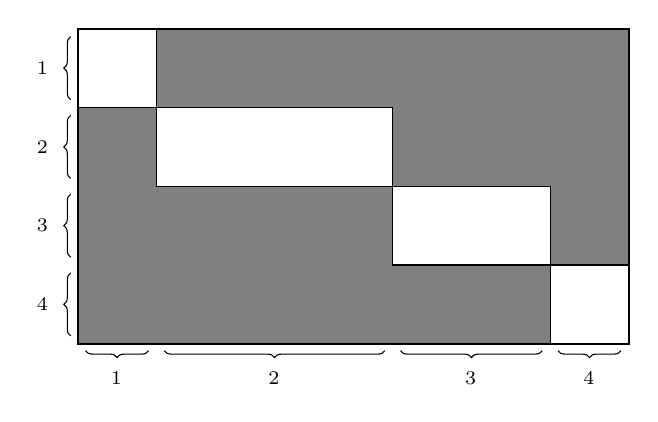
\begin{tikzpicture}
%\draw [fill=black] (0,0) rectangle (8,4);

\fill [gray] (0,0) rectangle (7,4);

\draw [fill=white] (0,4) rectangle (1,3);
\draw [fill=white] (1,3) rectangle (4,2);
\draw [fill=white] (4,2) rectangle (6,1);
\draw [fill=white] (6,1) rectangle (7,0);

\draw [thick] (0,0) rectangle (7,4);

%\node at (-.5, 3.5) {$\mcZ_1$};
%\node at (-.5, 2.5) {$\mcZ_2$};
%\node at (-.5, 1.5) {$\mcZ_3$};
%\node at (-.5, .5) {$\mcZ_4$};

%\node at (.5, -.5) {$\mcX_1$};
%\node at (2.5, -.5) {$\mcX_2$};
%\node at (5, -.5) {$\mcX_3$};
%\node at (6.5, -.5) {$\mcX_4$};

\draw[decorate,decoration={brace,mirror},xshift=-0.25em] (0,3.9) -- (0,3.1) node[midway,xshift=-1em] {$\mcZ_1$};
\draw[decorate,decoration={brace,mirror},xshift=-0.25em] (0,2.9) -- (0,2.1) node[midway,xshift=-1em] {$\mcZ_2$};
\draw[decorate,decoration={brace,mirror},xshift=-0.25em] (0,1.9) -- (0,1.1) node[midway,xshift=-1em] {$\mcZ_3$};
\draw[decorate,decoration={brace,mirror},xshift=-0.25em] (0,.9) -- (0,.1) node[midway,xshift=-1em] {$\mcZ_4$};

\draw[decorate,decoration={brace,mirror},yshift=-0.25em] (.1,0) -- (.9,0) node[midway,yshift=-1em] {$\mcX_1$};
\draw[decorate,decoration={brace,mirror},yshift=-0.25em] (1.1,0) -- (3.9,0) node[midway,yshift=-1em] {$\mcX_2$};
\draw[decorate,decoration={brace,mirror},yshift=-0.25em] (4.1,0) -- (5.9,0) node[midway,yshift=-1em] {$\mcX_3$};
\draw[decorate,decoration={brace,mirror},yshift=-0.25em] (6.1,0) -- (6.9,0) node[midway,yshift=-1em] {$\mcX_4$};

\end{tikzpicture}
}
\end{figure}
\end{center}

\end{frame}

\begin{comment}
\begin{frame}
\frametitle{Block-Sparse Emissions: Inference}

Given each word $x_t$, only the states in the correct group can occur
\vspace{1em} 

\begin{figure}
\captionsetup[subfigure]{justification=centering}
\begin{center}
\begin{subfigure}[t]{0.45\textwidth}
\centering
\resizebox{0.75\width}{0.75\height}{
\normalsize%
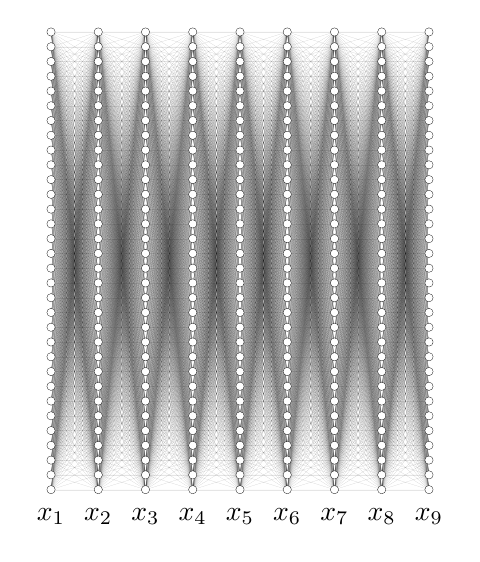
\begin{tikzpicture}%
\path[draw,line width=0.1pt,opacity=0.1,fill=black] (0.6,0.0) -- (1.2,0.0);%
\path[draw,line width=0.1pt,opacity=0.1,fill=black] (0.6,0.0) -- (1.2,0.1875);%
\path[draw,line width=0.1pt,opacity=0.1,fill=black] (0.6,0.0) -- (1.2,0.375);%
\path[draw,line width=0.1pt,opacity=0.1,fill=black] (0.6,0.0) -- (1.2,0.5625);%
\path[draw,line width=0.1pt,opacity=0.1,fill=black] (0.6,0.0) -- (1.2,0.75);%
\path[draw,line width=0.1pt,opacity=0.1,fill=black] (0.6,0.0) -- (1.2,0.9375);%
\path[draw,line width=0.1pt,opacity=0.1,fill=black] (0.6,0.0) -- (1.2,1.125);%
\path[draw,line width=0.1pt,opacity=0.1,fill=black] (0.6,0.0) -- (1.2,1.3125);%
\path[draw,line width=0.1pt,opacity=0.1,fill=black] (0.6,0.0) -- (1.2,1.5);%
\path[draw,line width=0.1pt,opacity=0.1,fill=black] (0.6,0.0) -- (1.2,1.6875);%
\path[draw,line width=0.1pt,opacity=0.1,fill=black] (0.6,0.0) -- (1.2,1.875);%
\path[draw,line width=0.1pt,opacity=0.1,fill=black] (0.6,0.0) -- (1.2,2.0625);%
\path[draw,line width=0.1pt,opacity=0.1,fill=black] (0.6,0.0) -- (1.2,2.25);%
\path[draw,line width=0.1pt,opacity=0.1,fill=black] (0.6,0.0) -- (1.2,2.4375);%
\path[draw,line width=0.1pt,opacity=0.1,fill=black] (0.6,0.0) -- (1.2,2.625);%
\path[draw,line width=0.1pt,opacity=0.1,fill=black] (0.6,0.0) -- (1.2,2.8125);%
\path[draw,line width=0.1pt,opacity=0.1,fill=black] (0.6,0.0) -- (1.2,3.0);%
\path[draw,line width=0.1pt,opacity=0.1,fill=black] (0.6,0.0) -- (1.2,3.1875);%
\path[draw,line width=0.1pt,opacity=0.1,fill=black] (0.6,0.0) -- (1.2,3.375);%
\path[draw,line width=0.1pt,opacity=0.1,fill=black] (0.6,0.0) -- (1.2,3.5625);%
\path[draw,line width=0.1pt,opacity=0.1,fill=black] (0.6,0.0) -- (1.2,3.75);%
\path[draw,line width=0.1pt,opacity=0.1,fill=black] (0.6,0.0) -- (1.2,3.9375);%
\path[draw,line width=0.1pt,opacity=0.1,fill=black] (0.6,0.0) -- (1.2,4.125);%
\path[draw,line width=0.1pt,opacity=0.1,fill=black] (0.6,0.0) -- (1.2,4.3125);%
\path[draw,line width=0.1pt,opacity=0.1,fill=black] (0.6,0.0) -- (1.2,4.5);%
\path[draw,line width=0.1pt,opacity=0.1,fill=black] (0.6,0.0) -- (1.2,4.6875);%
\path[draw,line width=0.1pt,opacity=0.1,fill=black] (0.6,0.0) -- (1.2,4.875);%
\path[draw,line width=0.1pt,opacity=0.1,fill=black] (0.6,0.0) -- (1.2,5.0625);%
\path[draw,line width=0.1pt,opacity=0.1,fill=black] (0.6,0.0) -- (1.2,5.25);%
\path[draw,line width=0.1pt,opacity=0.1,fill=black] (0.6,0.0) -- (1.2,5.4375);%
\path[draw,line width=0.1pt,opacity=0.1,fill=black] (0.6,0.0) -- (1.2,5.625);%
\path[draw,line width=0.1pt,opacity=0.1,fill=black] (0.6,0.0) -- (1.2,5.8125);%
\path[draw,line width=0.1pt,opacity=0.1,fill=black] (0.6,0.1875) -- (1.2,0.0);%
\path[draw,line width=0.1pt,opacity=0.1,fill=black] (0.6,0.1875) -- (1.2,0.1875);%
\path[draw,line width=0.1pt,opacity=0.1,fill=black] (0.6,0.1875) -- (1.2,0.375);%
\path[draw,line width=0.1pt,opacity=0.1,fill=black] (0.6,0.1875) -- (1.2,0.5625);%
\path[draw,line width=0.1pt,opacity=0.1,fill=black] (0.6,0.1875) -- (1.2,0.75);%
\path[draw,line width=0.1pt,opacity=0.1,fill=black] (0.6,0.1875) -- (1.2,0.9375);%
\path[draw,line width=0.1pt,opacity=0.1,fill=black] (0.6,0.1875) -- (1.2,1.125);%
\path[draw,line width=0.1pt,opacity=0.1,fill=black] (0.6,0.1875) -- (1.2,1.3125);%
\path[draw,line width=0.1pt,opacity=0.1,fill=black] (0.6,0.1875) -- (1.2,1.5);%
\path[draw,line width=0.1pt,opacity=0.1,fill=black] (0.6,0.1875) -- (1.2,1.6875);%
\path[draw,line width=0.1pt,opacity=0.1,fill=black] (0.6,0.1875) -- (1.2,1.875);%
\path[draw,line width=0.1pt,opacity=0.1,fill=black] (0.6,0.1875) -- (1.2,2.0625);%
\path[draw,line width=0.1pt,opacity=0.1,fill=black] (0.6,0.1875) -- (1.2,2.25);%
\path[draw,line width=0.1pt,opacity=0.1,fill=black] (0.6,0.1875) -- (1.2,2.4375);%
\path[draw,line width=0.1pt,opacity=0.1,fill=black] (0.6,0.1875) -- (1.2,2.625);%
\path[draw,line width=0.1pt,opacity=0.1,fill=black] (0.6,0.1875) -- (1.2,2.8125);%
\path[draw,line width=0.1pt,opacity=0.1,fill=black] (0.6,0.1875) -- (1.2,3.0);%
\path[draw,line width=0.1pt,opacity=0.1,fill=black] (0.6,0.1875) -- (1.2,3.1875);%
\path[draw,line width=0.1pt,opacity=0.1,fill=black] (0.6,0.1875) -- (1.2,3.375);%
\path[draw,line width=0.1pt,opacity=0.1,fill=black] (0.6,0.1875) -- (1.2,3.5625);%
\path[draw,line width=0.1pt,opacity=0.1,fill=black] (0.6,0.1875) -- (1.2,3.75);%
\path[draw,line width=0.1pt,opacity=0.1,fill=black] (0.6,0.1875) -- (1.2,3.9375);%
\path[draw,line width=0.1pt,opacity=0.1,fill=black] (0.6,0.1875) -- (1.2,4.125);%
\path[draw,line width=0.1pt,opacity=0.1,fill=black] (0.6,0.1875) -- (1.2,4.3125);%
\path[draw,line width=0.1pt,opacity=0.1,fill=black] (0.6,0.1875) -- (1.2,4.5);%
\path[draw,line width=0.1pt,opacity=0.1,fill=black] (0.6,0.1875) -- (1.2,4.6875);%
\path[draw,line width=0.1pt,opacity=0.1,fill=black] (0.6,0.1875) -- (1.2,4.875);%
\path[draw,line width=0.1pt,opacity=0.1,fill=black] (0.6,0.1875) -- (1.2,5.0625);%
\path[draw,line width=0.1pt,opacity=0.1,fill=black] (0.6,0.1875) -- (1.2,5.25);%
\path[draw,line width=0.1pt,opacity=0.1,fill=black] (0.6,0.1875) -- (1.2,5.4375);%
\path[draw,line width=0.1pt,opacity=0.1,fill=black] (0.6,0.1875) -- (1.2,5.625);%
\path[draw,line width=0.1pt,opacity=0.1,fill=black] (0.6,0.1875) -- (1.2,5.8125);%
\path[draw,line width=0.1pt,opacity=0.1,fill=black] (0.6,0.375) -- (1.2,0.0);%
\path[draw,line width=0.1pt,opacity=0.1,fill=black] (0.6,0.375) -- (1.2,0.1875);%
\path[draw,line width=0.1pt,opacity=0.1,fill=black] (0.6,0.375) -- (1.2,0.375);%
\path[draw,line width=0.1pt,opacity=0.1,fill=black] (0.6,0.375) -- (1.2,0.5625);%
\path[draw,line width=0.1pt,opacity=0.1,fill=black] (0.6,0.375) -- (1.2,0.75);%
\path[draw,line width=0.1pt,opacity=0.1,fill=black] (0.6,0.375) -- (1.2,0.9375);%
\path[draw,line width=0.1pt,opacity=0.1,fill=black] (0.6,0.375) -- (1.2,1.125);%
\path[draw,line width=0.1pt,opacity=0.1,fill=black] (0.6,0.375) -- (1.2,1.3125);%
\path[draw,line width=0.1pt,opacity=0.1,fill=black] (0.6,0.375) -- (1.2,1.5);%
\path[draw,line width=0.1pt,opacity=0.1,fill=black] (0.6,0.375) -- (1.2,1.6875);%
\path[draw,line width=0.1pt,opacity=0.1,fill=black] (0.6,0.375) -- (1.2,1.875);%
\path[draw,line width=0.1pt,opacity=0.1,fill=black] (0.6,0.375) -- (1.2,2.0625);%
\path[draw,line width=0.1pt,opacity=0.1,fill=black] (0.6,0.375) -- (1.2,2.25);%
\path[draw,line width=0.1pt,opacity=0.1,fill=black] (0.6,0.375) -- (1.2,2.4375);%
\path[draw,line width=0.1pt,opacity=0.1,fill=black] (0.6,0.375) -- (1.2,2.625);%
\path[draw,line width=0.1pt,opacity=0.1,fill=black] (0.6,0.375) -- (1.2,2.8125);%
\path[draw,line width=0.1pt,opacity=0.1,fill=black] (0.6,0.375) -- (1.2,3.0);%
\path[draw,line width=0.1pt,opacity=0.1,fill=black] (0.6,0.375) -- (1.2,3.1875);%
\path[draw,line width=0.1pt,opacity=0.1,fill=black] (0.6,0.375) -- (1.2,3.375);%
\path[draw,line width=0.1pt,opacity=0.1,fill=black] (0.6,0.375) -- (1.2,3.5625);%
\path[draw,line width=0.1pt,opacity=0.1,fill=black] (0.6,0.375) -- (1.2,3.75);%
\path[draw,line width=0.1pt,opacity=0.1,fill=black] (0.6,0.375) -- (1.2,3.9375);%
\path[draw,line width=0.1pt,opacity=0.1,fill=black] (0.6,0.375) -- (1.2,4.125);%
\path[draw,line width=0.1pt,opacity=0.1,fill=black] (0.6,0.375) -- (1.2,4.3125);%
\path[draw,line width=0.1pt,opacity=0.1,fill=black] (0.6,0.375) -- (1.2,4.5);%
\path[draw,line width=0.1pt,opacity=0.1,fill=black] (0.6,0.375) -- (1.2,4.6875);%
\path[draw,line width=0.1pt,opacity=0.1,fill=black] (0.6,0.375) -- (1.2,4.875);%
\path[draw,line width=0.1pt,opacity=0.1,fill=black] (0.6,0.375) -- (1.2,5.0625);%
\path[draw,line width=0.1pt,opacity=0.1,fill=black] (0.6,0.375) -- (1.2,5.25);%
\path[draw,line width=0.1pt,opacity=0.1,fill=black] (0.6,0.375) -- (1.2,5.4375);%
\path[draw,line width=0.1pt,opacity=0.1,fill=black] (0.6,0.375) -- (1.2,5.625);%
\path[draw,line width=0.1pt,opacity=0.1,fill=black] (0.6,0.375) -- (1.2,5.8125);%
\path[draw,line width=0.1pt,opacity=0.1,fill=black] (0.6,0.5625) -- (1.2,0.0);%
\path[draw,line width=0.1pt,opacity=0.1,fill=black] (0.6,0.5625) -- (1.2,0.1875);%
\path[draw,line width=0.1pt,opacity=0.1,fill=black] (0.6,0.5625) -- (1.2,0.375);%
\path[draw,line width=0.1pt,opacity=0.1,fill=black] (0.6,0.5625) -- (1.2,0.5625);%
\path[draw,line width=0.1pt,opacity=0.1,fill=black] (0.6,0.5625) -- (1.2,0.75);%
\path[draw,line width=0.1pt,opacity=0.1,fill=black] (0.6,0.5625) -- (1.2,0.9375);%
\path[draw,line width=0.1pt,opacity=0.1,fill=black] (0.6,0.5625) -- (1.2,1.125);%
\path[draw,line width=0.1pt,opacity=0.1,fill=black] (0.6,0.5625) -- (1.2,1.3125);%
\path[draw,line width=0.1pt,opacity=0.1,fill=black] (0.6,0.5625) -- (1.2,1.5);%
\path[draw,line width=0.1pt,opacity=0.1,fill=black] (0.6,0.5625) -- (1.2,1.6875);%
\path[draw,line width=0.1pt,opacity=0.1,fill=black] (0.6,0.5625) -- (1.2,1.875);%
\path[draw,line width=0.1pt,opacity=0.1,fill=black] (0.6,0.5625) -- (1.2,2.0625);%
\path[draw,line width=0.1pt,opacity=0.1,fill=black] (0.6,0.5625) -- (1.2,2.25);%
\path[draw,line width=0.1pt,opacity=0.1,fill=black] (0.6,0.5625) -- (1.2,2.4375);%
\path[draw,line width=0.1pt,opacity=0.1,fill=black] (0.6,0.5625) -- (1.2,2.625);%
\path[draw,line width=0.1pt,opacity=0.1,fill=black] (0.6,0.5625) -- (1.2,2.8125);%
\path[draw,line width=0.1pt,opacity=0.1,fill=black] (0.6,0.5625) -- (1.2,3.0);%
\path[draw,line width=0.1pt,opacity=0.1,fill=black] (0.6,0.5625) -- (1.2,3.1875);%
\path[draw,line width=0.1pt,opacity=0.1,fill=black] (0.6,0.5625) -- (1.2,3.375);%
\path[draw,line width=0.1pt,opacity=0.1,fill=black] (0.6,0.5625) -- (1.2,3.5625);%
\path[draw,line width=0.1pt,opacity=0.1,fill=black] (0.6,0.5625) -- (1.2,3.75);%
\path[draw,line width=0.1pt,opacity=0.1,fill=black] (0.6,0.5625) -- (1.2,3.9375);%
\path[draw,line width=0.1pt,opacity=0.1,fill=black] (0.6,0.5625) -- (1.2,4.125);%
\path[draw,line width=0.1pt,opacity=0.1,fill=black] (0.6,0.5625) -- (1.2,4.3125);%
\path[draw,line width=0.1pt,opacity=0.1,fill=black] (0.6,0.5625) -- (1.2,4.5);%
\path[draw,line width=0.1pt,opacity=0.1,fill=black] (0.6,0.5625) -- (1.2,4.6875);%
\path[draw,line width=0.1pt,opacity=0.1,fill=black] (0.6,0.5625) -- (1.2,4.875);%
\path[draw,line width=0.1pt,opacity=0.1,fill=black] (0.6,0.5625) -- (1.2,5.0625);%
\path[draw,line width=0.1pt,opacity=0.1,fill=black] (0.6,0.5625) -- (1.2,5.25);%
\path[draw,line width=0.1pt,opacity=0.1,fill=black] (0.6,0.5625) -- (1.2,5.4375);%
\path[draw,line width=0.1pt,opacity=0.1,fill=black] (0.6,0.5625) -- (1.2,5.625);%
\path[draw,line width=0.1pt,opacity=0.1,fill=black] (0.6,0.5625) -- (1.2,5.8125);%
\path[draw,line width=0.1pt,opacity=0.1,fill=black] (0.6,0.75) -- (1.2,0.0);%
\path[draw,line width=0.1pt,opacity=0.1,fill=black] (0.6,0.75) -- (1.2,0.1875);%
\path[draw,line width=0.1pt,opacity=0.1,fill=black] (0.6,0.75) -- (1.2,0.375);%
\path[draw,line width=0.1pt,opacity=0.1,fill=black] (0.6,0.75) -- (1.2,0.5625);%
\path[draw,line width=0.1pt,opacity=0.1,fill=black] (0.6,0.75) -- (1.2,0.75);%
\path[draw,line width=0.1pt,opacity=0.1,fill=black] (0.6,0.75) -- (1.2,0.9375);%
\path[draw,line width=0.1pt,opacity=0.1,fill=black] (0.6,0.75) -- (1.2,1.125);%
\path[draw,line width=0.1pt,opacity=0.1,fill=black] (0.6,0.75) -- (1.2,1.3125);%
\path[draw,line width=0.1pt,opacity=0.1,fill=black] (0.6,0.75) -- (1.2,1.5);%
\path[draw,line width=0.1pt,opacity=0.1,fill=black] (0.6,0.75) -- (1.2,1.6875);%
\path[draw,line width=0.1pt,opacity=0.1,fill=black] (0.6,0.75) -- (1.2,1.875);%
\path[draw,line width=0.1pt,opacity=0.1,fill=black] (0.6,0.75) -- (1.2,2.0625);%
\path[draw,line width=0.1pt,opacity=0.1,fill=black] (0.6,0.75) -- (1.2,2.25);%
\path[draw,line width=0.1pt,opacity=0.1,fill=black] (0.6,0.75) -- (1.2,2.4375);%
\path[draw,line width=0.1pt,opacity=0.1,fill=black] (0.6,0.75) -- (1.2,2.625);%
\path[draw,line width=0.1pt,opacity=0.1,fill=black] (0.6,0.75) -- (1.2,2.8125);%
\path[draw,line width=0.1pt,opacity=0.1,fill=black] (0.6,0.75) -- (1.2,3.0);%
\path[draw,line width=0.1pt,opacity=0.1,fill=black] (0.6,0.75) -- (1.2,3.1875);%
\path[draw,line width=0.1pt,opacity=0.1,fill=black] (0.6,0.75) -- (1.2,3.375);%
\path[draw,line width=0.1pt,opacity=0.1,fill=black] (0.6,0.75) -- (1.2,3.5625);%
\path[draw,line width=0.1pt,opacity=0.1,fill=black] (0.6,0.75) -- (1.2,3.75);%
\path[draw,line width=0.1pt,opacity=0.1,fill=black] (0.6,0.75) -- (1.2,3.9375);%
\path[draw,line width=0.1pt,opacity=0.1,fill=black] (0.6,0.75) -- (1.2,4.125);%
\path[draw,line width=0.1pt,opacity=0.1,fill=black] (0.6,0.75) -- (1.2,4.3125);%
\path[draw,line width=0.1pt,opacity=0.1,fill=black] (0.6,0.75) -- (1.2,4.5);%
\path[draw,line width=0.1pt,opacity=0.1,fill=black] (0.6,0.75) -- (1.2,4.6875);%
\path[draw,line width=0.1pt,opacity=0.1,fill=black] (0.6,0.75) -- (1.2,4.875);%
\path[draw,line width=0.1pt,opacity=0.1,fill=black] (0.6,0.75) -- (1.2,5.0625);%
\path[draw,line width=0.1pt,opacity=0.1,fill=black] (0.6,0.75) -- (1.2,5.25);%
\path[draw,line width=0.1pt,opacity=0.1,fill=black] (0.6,0.75) -- (1.2,5.4375);%
\path[draw,line width=0.1pt,opacity=0.1,fill=black] (0.6,0.75) -- (1.2,5.625);%
\path[draw,line width=0.1pt,opacity=0.1,fill=black] (0.6,0.75) -- (1.2,5.8125);%
\path[draw,line width=0.1pt,opacity=0.1,fill=black] (0.6,0.9375) -- (1.2,0.0);%
\path[draw,line width=0.1pt,opacity=0.1,fill=black] (0.6,0.9375) -- (1.2,0.1875);%
\path[draw,line width=0.1pt,opacity=0.1,fill=black] (0.6,0.9375) -- (1.2,0.375);%
\path[draw,line width=0.1pt,opacity=0.1,fill=black] (0.6,0.9375) -- (1.2,0.5625);%
\path[draw,line width=0.1pt,opacity=0.1,fill=black] (0.6,0.9375) -- (1.2,0.75);%
\path[draw,line width=0.1pt,opacity=0.1,fill=black] (0.6,0.9375) -- (1.2,0.9375);%
\path[draw,line width=0.1pt,opacity=0.1,fill=black] (0.6,0.9375) -- (1.2,1.125);%
\path[draw,line width=0.1pt,opacity=0.1,fill=black] (0.6,0.9375) -- (1.2,1.3125);%
\path[draw,line width=0.1pt,opacity=0.1,fill=black] (0.6,0.9375) -- (1.2,1.5);%
\path[draw,line width=0.1pt,opacity=0.1,fill=black] (0.6,0.9375) -- (1.2,1.6875);%
\path[draw,line width=0.1pt,opacity=0.1,fill=black] (0.6,0.9375) -- (1.2,1.875);%
\path[draw,line width=0.1pt,opacity=0.1,fill=black] (0.6,0.9375) -- (1.2,2.0625);%
\path[draw,line width=0.1pt,opacity=0.1,fill=black] (0.6,0.9375) -- (1.2,2.25);%
\path[draw,line width=0.1pt,opacity=0.1,fill=black] (0.6,0.9375) -- (1.2,2.4375);%
\path[draw,line width=0.1pt,opacity=0.1,fill=black] (0.6,0.9375) -- (1.2,2.625);%
\path[draw,line width=0.1pt,opacity=0.1,fill=black] (0.6,0.9375) -- (1.2,2.8125);%
\path[draw,line width=0.1pt,opacity=0.1,fill=black] (0.6,0.9375) -- (1.2,3.0);%
\path[draw,line width=0.1pt,opacity=0.1,fill=black] (0.6,0.9375) -- (1.2,3.1875);%
\path[draw,line width=0.1pt,opacity=0.1,fill=black] (0.6,0.9375) -- (1.2,3.375);%
\path[draw,line width=0.1pt,opacity=0.1,fill=black] (0.6,0.9375) -- (1.2,3.5625);%
\path[draw,line width=0.1pt,opacity=0.1,fill=black] (0.6,0.9375) -- (1.2,3.75);%
\path[draw,line width=0.1pt,opacity=0.1,fill=black] (0.6,0.9375) -- (1.2,3.9375);%
\path[draw,line width=0.1pt,opacity=0.1,fill=black] (0.6,0.9375) -- (1.2,4.125);%
\path[draw,line width=0.1pt,opacity=0.1,fill=black] (0.6,0.9375) -- (1.2,4.3125);%
\path[draw,line width=0.1pt,opacity=0.1,fill=black] (0.6,0.9375) -- (1.2,4.5);%
\path[draw,line width=0.1pt,opacity=0.1,fill=black] (0.6,0.9375) -- (1.2,4.6875);%
\path[draw,line width=0.1pt,opacity=0.1,fill=black] (0.6,0.9375) -- (1.2,4.875);%
\path[draw,line width=0.1pt,opacity=0.1,fill=black] (0.6,0.9375) -- (1.2,5.0625);%
\path[draw,line width=0.1pt,opacity=0.1,fill=black] (0.6,0.9375) -- (1.2,5.25);%
\path[draw,line width=0.1pt,opacity=0.1,fill=black] (0.6,0.9375) -- (1.2,5.4375);%
\path[draw,line width=0.1pt,opacity=0.1,fill=black] (0.6,0.9375) -- (1.2,5.625);%
\path[draw,line width=0.1pt,opacity=0.1,fill=black] (0.6,0.9375) -- (1.2,5.8125);%
\path[draw,line width=0.1pt,opacity=0.1,fill=black] (0.6,1.125) -- (1.2,0.0);%
\path[draw,line width=0.1pt,opacity=0.1,fill=black] (0.6,1.125) -- (1.2,0.1875);%
\path[draw,line width=0.1pt,opacity=0.1,fill=black] (0.6,1.125) -- (1.2,0.375);%
\path[draw,line width=0.1pt,opacity=0.1,fill=black] (0.6,1.125) -- (1.2,0.5625);%
\path[draw,line width=0.1pt,opacity=0.1,fill=black] (0.6,1.125) -- (1.2,0.75);%
\path[draw,line width=0.1pt,opacity=0.1,fill=black] (0.6,1.125) -- (1.2,0.9375);%
\path[draw,line width=0.1pt,opacity=0.1,fill=black] (0.6,1.125) -- (1.2,1.125);%
\path[draw,line width=0.1pt,opacity=0.1,fill=black] (0.6,1.125) -- (1.2,1.3125);%
\path[draw,line width=0.1pt,opacity=0.1,fill=black] (0.6,1.125) -- (1.2,1.5);%
\path[draw,line width=0.1pt,opacity=0.1,fill=black] (0.6,1.125) -- (1.2,1.6875);%
\path[draw,line width=0.1pt,opacity=0.1,fill=black] (0.6,1.125) -- (1.2,1.875);%
\path[draw,line width=0.1pt,opacity=0.1,fill=black] (0.6,1.125) -- (1.2,2.0625);%
\path[draw,line width=0.1pt,opacity=0.1,fill=black] (0.6,1.125) -- (1.2,2.25);%
\path[draw,line width=0.1pt,opacity=0.1,fill=black] (0.6,1.125) -- (1.2,2.4375);%
\path[draw,line width=0.1pt,opacity=0.1,fill=black] (0.6,1.125) -- (1.2,2.625);%
\path[draw,line width=0.1pt,opacity=0.1,fill=black] (0.6,1.125) -- (1.2,2.8125);%
\path[draw,line width=0.1pt,opacity=0.1,fill=black] (0.6,1.125) -- (1.2,3.0);%
\path[draw,line width=0.1pt,opacity=0.1,fill=black] (0.6,1.125) -- (1.2,3.1875);%
\path[draw,line width=0.1pt,opacity=0.1,fill=black] (0.6,1.125) -- (1.2,3.375);%
\path[draw,line width=0.1pt,opacity=0.1,fill=black] (0.6,1.125) -- (1.2,3.5625);%
\path[draw,line width=0.1pt,opacity=0.1,fill=black] (0.6,1.125) -- (1.2,3.75);%
\path[draw,line width=0.1pt,opacity=0.1,fill=black] (0.6,1.125) -- (1.2,3.9375);%
\path[draw,line width=0.1pt,opacity=0.1,fill=black] (0.6,1.125) -- (1.2,4.125);%
\path[draw,line width=0.1pt,opacity=0.1,fill=black] (0.6,1.125) -- (1.2,4.3125);%
\path[draw,line width=0.1pt,opacity=0.1,fill=black] (0.6,1.125) -- (1.2,4.5);%
\path[draw,line width=0.1pt,opacity=0.1,fill=black] (0.6,1.125) -- (1.2,4.6875);%
\path[draw,line width=0.1pt,opacity=0.1,fill=black] (0.6,1.125) -- (1.2,4.875);%
\path[draw,line width=0.1pt,opacity=0.1,fill=black] (0.6,1.125) -- (1.2,5.0625);%
\path[draw,line width=0.1pt,opacity=0.1,fill=black] (0.6,1.125) -- (1.2,5.25);%
\path[draw,line width=0.1pt,opacity=0.1,fill=black] (0.6,1.125) -- (1.2,5.4375);%
\path[draw,line width=0.1pt,opacity=0.1,fill=black] (0.6,1.125) -- (1.2,5.625);%
\path[draw,line width=0.1pt,opacity=0.1,fill=black] (0.6,1.125) -- (1.2,5.8125);%
\path[draw,line width=0.1pt,opacity=0.1,fill=black] (0.6,1.3125) -- (1.2,0.0);%
\path[draw,line width=0.1pt,opacity=0.1,fill=black] (0.6,1.3125) -- (1.2,0.1875);%
\path[draw,line width=0.1pt,opacity=0.1,fill=black] (0.6,1.3125) -- (1.2,0.375);%
\path[draw,line width=0.1pt,opacity=0.1,fill=black] (0.6,1.3125) -- (1.2,0.5625);%
\path[draw,line width=0.1pt,opacity=0.1,fill=black] (0.6,1.3125) -- (1.2,0.75);%
\path[draw,line width=0.1pt,opacity=0.1,fill=black] (0.6,1.3125) -- (1.2,0.9375);%
\path[draw,line width=0.1pt,opacity=0.1,fill=black] (0.6,1.3125) -- (1.2,1.125);%
\path[draw,line width=0.1pt,opacity=0.1,fill=black] (0.6,1.3125) -- (1.2,1.3125);%
\path[draw,line width=0.1pt,opacity=0.1,fill=black] (0.6,1.3125) -- (1.2,1.5);%
\path[draw,line width=0.1pt,opacity=0.1,fill=black] (0.6,1.3125) -- (1.2,1.6875);%
\path[draw,line width=0.1pt,opacity=0.1,fill=black] (0.6,1.3125) -- (1.2,1.875);%
\path[draw,line width=0.1pt,opacity=0.1,fill=black] (0.6,1.3125) -- (1.2,2.0625);%
\path[draw,line width=0.1pt,opacity=0.1,fill=black] (0.6,1.3125) -- (1.2,2.25);%
\path[draw,line width=0.1pt,opacity=0.1,fill=black] (0.6,1.3125) -- (1.2,2.4375);%
\path[draw,line width=0.1pt,opacity=0.1,fill=black] (0.6,1.3125) -- (1.2,2.625);%
\path[draw,line width=0.1pt,opacity=0.1,fill=black] (0.6,1.3125) -- (1.2,2.8125);%
\path[draw,line width=0.1pt,opacity=0.1,fill=black] (0.6,1.3125) -- (1.2,3.0);%
\path[draw,line width=0.1pt,opacity=0.1,fill=black] (0.6,1.3125) -- (1.2,3.1875);%
\path[draw,line width=0.1pt,opacity=0.1,fill=black] (0.6,1.3125) -- (1.2,3.375);%
\path[draw,line width=0.1pt,opacity=0.1,fill=black] (0.6,1.3125) -- (1.2,3.5625);%
\path[draw,line width=0.1pt,opacity=0.1,fill=black] (0.6,1.3125) -- (1.2,3.75);%
\path[draw,line width=0.1pt,opacity=0.1,fill=black] (0.6,1.3125) -- (1.2,3.9375);%
\path[draw,line width=0.1pt,opacity=0.1,fill=black] (0.6,1.3125) -- (1.2,4.125);%
\path[draw,line width=0.1pt,opacity=0.1,fill=black] (0.6,1.3125) -- (1.2,4.3125);%
\path[draw,line width=0.1pt,opacity=0.1,fill=black] (0.6,1.3125) -- (1.2,4.5);%
\path[draw,line width=0.1pt,opacity=0.1,fill=black] (0.6,1.3125) -- (1.2,4.6875);%
\path[draw,line width=0.1pt,opacity=0.1,fill=black] (0.6,1.3125) -- (1.2,4.875);%
\path[draw,line width=0.1pt,opacity=0.1,fill=black] (0.6,1.3125) -- (1.2,5.0625);%
\path[draw,line width=0.1pt,opacity=0.1,fill=black] (0.6,1.3125) -- (1.2,5.25);%
\path[draw,line width=0.1pt,opacity=0.1,fill=black] (0.6,1.3125) -- (1.2,5.4375);%
\path[draw,line width=0.1pt,opacity=0.1,fill=black] (0.6,1.3125) -- (1.2,5.625);%
\path[draw,line width=0.1pt,opacity=0.1,fill=black] (0.6,1.3125) -- (1.2,5.8125);%
\path[draw,line width=0.1pt,opacity=0.1,fill=black] (0.6,1.5) -- (1.2,0.0);%
\path[draw,line width=0.1pt,opacity=0.1,fill=black] (0.6,1.5) -- (1.2,0.1875);%
\path[draw,line width=0.1pt,opacity=0.1,fill=black] (0.6,1.5) -- (1.2,0.375);%
\path[draw,line width=0.1pt,opacity=0.1,fill=black] (0.6,1.5) -- (1.2,0.5625);%
\path[draw,line width=0.1pt,opacity=0.1,fill=black] (0.6,1.5) -- (1.2,0.75);%
\path[draw,line width=0.1pt,opacity=0.1,fill=black] (0.6,1.5) -- (1.2,0.9375);%
\path[draw,line width=0.1pt,opacity=0.1,fill=black] (0.6,1.5) -- (1.2,1.125);%
\path[draw,line width=0.1pt,opacity=0.1,fill=black] (0.6,1.5) -- (1.2,1.3125);%
\path[draw,line width=0.1pt,opacity=0.1,fill=black] (0.6,1.5) -- (1.2,1.5);%
\path[draw,line width=0.1pt,opacity=0.1,fill=black] (0.6,1.5) -- (1.2,1.6875);%
\path[draw,line width=0.1pt,opacity=0.1,fill=black] (0.6,1.5) -- (1.2,1.875);%
\path[draw,line width=0.1pt,opacity=0.1,fill=black] (0.6,1.5) -- (1.2,2.0625);%
\path[draw,line width=0.1pt,opacity=0.1,fill=black] (0.6,1.5) -- (1.2,2.25);%
\path[draw,line width=0.1pt,opacity=0.1,fill=black] (0.6,1.5) -- (1.2,2.4375);%
\path[draw,line width=0.1pt,opacity=0.1,fill=black] (0.6,1.5) -- (1.2,2.625);%
\path[draw,line width=0.1pt,opacity=0.1,fill=black] (0.6,1.5) -- (1.2,2.8125);%
\path[draw,line width=0.1pt,opacity=0.1,fill=black] (0.6,1.5) -- (1.2,3.0);%
\path[draw,line width=0.1pt,opacity=0.1,fill=black] (0.6,1.5) -- (1.2,3.1875);%
\path[draw,line width=0.1pt,opacity=0.1,fill=black] (0.6,1.5) -- (1.2,3.375);%
\path[draw,line width=0.1pt,opacity=0.1,fill=black] (0.6,1.5) -- (1.2,3.5625);%
\path[draw,line width=0.1pt,opacity=0.1,fill=black] (0.6,1.5) -- (1.2,3.75);%
\path[draw,line width=0.1pt,opacity=0.1,fill=black] (0.6,1.5) -- (1.2,3.9375);%
\path[draw,line width=0.1pt,opacity=0.1,fill=black] (0.6,1.5) -- (1.2,4.125);%
\path[draw,line width=0.1pt,opacity=0.1,fill=black] (0.6,1.5) -- (1.2,4.3125);%
\path[draw,line width=0.1pt,opacity=0.1,fill=black] (0.6,1.5) -- (1.2,4.5);%
\path[draw,line width=0.1pt,opacity=0.1,fill=black] (0.6,1.5) -- (1.2,4.6875);%
\path[draw,line width=0.1pt,opacity=0.1,fill=black] (0.6,1.5) -- (1.2,4.875);%
\path[draw,line width=0.1pt,opacity=0.1,fill=black] (0.6,1.5) -- (1.2,5.0625);%
\path[draw,line width=0.1pt,opacity=0.1,fill=black] (0.6,1.5) -- (1.2,5.25);%
\path[draw,line width=0.1pt,opacity=0.1,fill=black] (0.6,1.5) -- (1.2,5.4375);%
\path[draw,line width=0.1pt,opacity=0.1,fill=black] (0.6,1.5) -- (1.2,5.625);%
\path[draw,line width=0.1pt,opacity=0.1,fill=black] (0.6,1.5) -- (1.2,5.8125);%
\path[draw,line width=0.1pt,opacity=0.1,fill=black] (0.6,1.6875) -- (1.2,0.0);%
\path[draw,line width=0.1pt,opacity=0.1,fill=black] (0.6,1.6875) -- (1.2,0.1875);%
\path[draw,line width=0.1pt,opacity=0.1,fill=black] (0.6,1.6875) -- (1.2,0.375);%
\path[draw,line width=0.1pt,opacity=0.1,fill=black] (0.6,1.6875) -- (1.2,0.5625);%
\path[draw,line width=0.1pt,opacity=0.1,fill=black] (0.6,1.6875) -- (1.2,0.75);%
\path[draw,line width=0.1pt,opacity=0.1,fill=black] (0.6,1.6875) -- (1.2,0.9375);%
\path[draw,line width=0.1pt,opacity=0.1,fill=black] (0.6,1.6875) -- (1.2,1.125);%
\path[draw,line width=0.1pt,opacity=0.1,fill=black] (0.6,1.6875) -- (1.2,1.3125);%
\path[draw,line width=0.1pt,opacity=0.1,fill=black] (0.6,1.6875) -- (1.2,1.5);%
\path[draw,line width=0.1pt,opacity=0.1,fill=black] (0.6,1.6875) -- (1.2,1.6875);%
\path[draw,line width=0.1pt,opacity=0.1,fill=black] (0.6,1.6875) -- (1.2,1.875);%
\path[draw,line width=0.1pt,opacity=0.1,fill=black] (0.6,1.6875) -- (1.2,2.0625);%
\path[draw,line width=0.1pt,opacity=0.1,fill=black] (0.6,1.6875) -- (1.2,2.25);%
\path[draw,line width=0.1pt,opacity=0.1,fill=black] (0.6,1.6875) -- (1.2,2.4375);%
\path[draw,line width=0.1pt,opacity=0.1,fill=black] (0.6,1.6875) -- (1.2,2.625);%
\path[draw,line width=0.1pt,opacity=0.1,fill=black] (0.6,1.6875) -- (1.2,2.8125);%
\path[draw,line width=0.1pt,opacity=0.1,fill=black] (0.6,1.6875) -- (1.2,3.0);%
\path[draw,line width=0.1pt,opacity=0.1,fill=black] (0.6,1.6875) -- (1.2,3.1875);%
\path[draw,line width=0.1pt,opacity=0.1,fill=black] (0.6,1.6875) -- (1.2,3.375);%
\path[draw,line width=0.1pt,opacity=0.1,fill=black] (0.6,1.6875) -- (1.2,3.5625);%
\path[draw,line width=0.1pt,opacity=0.1,fill=black] (0.6,1.6875) -- (1.2,3.75);%
\path[draw,line width=0.1pt,opacity=0.1,fill=black] (0.6,1.6875) -- (1.2,3.9375);%
\path[draw,line width=0.1pt,opacity=0.1,fill=black] (0.6,1.6875) -- (1.2,4.125);%
\path[draw,line width=0.1pt,opacity=0.1,fill=black] (0.6,1.6875) -- (1.2,4.3125);%
\path[draw,line width=0.1pt,opacity=0.1,fill=black] (0.6,1.6875) -- (1.2,4.5);%
\path[draw,line width=0.1pt,opacity=0.1,fill=black] (0.6,1.6875) -- (1.2,4.6875);%
\path[draw,line width=0.1pt,opacity=0.1,fill=black] (0.6,1.6875) -- (1.2,4.875);%
\path[draw,line width=0.1pt,opacity=0.1,fill=black] (0.6,1.6875) -- (1.2,5.0625);%
\path[draw,line width=0.1pt,opacity=0.1,fill=black] (0.6,1.6875) -- (1.2,5.25);%
\path[draw,line width=0.1pt,opacity=0.1,fill=black] (0.6,1.6875) -- (1.2,5.4375);%
\path[draw,line width=0.1pt,opacity=0.1,fill=black] (0.6,1.6875) -- (1.2,5.625);%
\path[draw,line width=0.1pt,opacity=0.1,fill=black] (0.6,1.6875) -- (1.2,5.8125);%
\path[draw,line width=0.1pt,opacity=0.1,fill=black] (0.6,1.875) -- (1.2,0.0);%
\path[draw,line width=0.1pt,opacity=0.1,fill=black] (0.6,1.875) -- (1.2,0.1875);%
\path[draw,line width=0.1pt,opacity=0.1,fill=black] (0.6,1.875) -- (1.2,0.375);%
\path[draw,line width=0.1pt,opacity=0.1,fill=black] (0.6,1.875) -- (1.2,0.5625);%
\path[draw,line width=0.1pt,opacity=0.1,fill=black] (0.6,1.875) -- (1.2,0.75);%
\path[draw,line width=0.1pt,opacity=0.1,fill=black] (0.6,1.875) -- (1.2,0.9375);%
\path[draw,line width=0.1pt,opacity=0.1,fill=black] (0.6,1.875) -- (1.2,1.125);%
\path[draw,line width=0.1pt,opacity=0.1,fill=black] (0.6,1.875) -- (1.2,1.3125);%
\path[draw,line width=0.1pt,opacity=0.1,fill=black] (0.6,1.875) -- (1.2,1.5);%
\path[draw,line width=0.1pt,opacity=0.1,fill=black] (0.6,1.875) -- (1.2,1.6875);%
\path[draw,line width=0.1pt,opacity=0.1,fill=black] (0.6,1.875) -- (1.2,1.875);%
\path[draw,line width=0.1pt,opacity=0.1,fill=black] (0.6,1.875) -- (1.2,2.0625);%
\path[draw,line width=0.1pt,opacity=0.1,fill=black] (0.6,1.875) -- (1.2,2.25);%
\path[draw,line width=0.1pt,opacity=0.1,fill=black] (0.6,1.875) -- (1.2,2.4375);%
\path[draw,line width=0.1pt,opacity=0.1,fill=black] (0.6,1.875) -- (1.2,2.625);%
\path[draw,line width=0.1pt,opacity=0.1,fill=black] (0.6,1.875) -- (1.2,2.8125);%
\path[draw,line width=0.1pt,opacity=0.1,fill=black] (0.6,1.875) -- (1.2,3.0);%
\path[draw,line width=0.1pt,opacity=0.1,fill=black] (0.6,1.875) -- (1.2,3.1875);%
\path[draw,line width=0.1pt,opacity=0.1,fill=black] (0.6,1.875) -- (1.2,3.375);%
\path[draw,line width=0.1pt,opacity=0.1,fill=black] (0.6,1.875) -- (1.2,3.5625);%
\path[draw,line width=0.1pt,opacity=0.1,fill=black] (0.6,1.875) -- (1.2,3.75);%
\path[draw,line width=0.1pt,opacity=0.1,fill=black] (0.6,1.875) -- (1.2,3.9375);%
\path[draw,line width=0.1pt,opacity=0.1,fill=black] (0.6,1.875) -- (1.2,4.125);%
\path[draw,line width=0.1pt,opacity=0.1,fill=black] (0.6,1.875) -- (1.2,4.3125);%
\path[draw,line width=0.1pt,opacity=0.1,fill=black] (0.6,1.875) -- (1.2,4.5);%
\path[draw,line width=0.1pt,opacity=0.1,fill=black] (0.6,1.875) -- (1.2,4.6875);%
\path[draw,line width=0.1pt,opacity=0.1,fill=black] (0.6,1.875) -- (1.2,4.875);%
\path[draw,line width=0.1pt,opacity=0.1,fill=black] (0.6,1.875) -- (1.2,5.0625);%
\path[draw,line width=0.1pt,opacity=0.1,fill=black] (0.6,1.875) -- (1.2,5.25);%
\path[draw,line width=0.1pt,opacity=0.1,fill=black] (0.6,1.875) -- (1.2,5.4375);%
\path[draw,line width=0.1pt,opacity=0.1,fill=black] (0.6,1.875) -- (1.2,5.625);%
\path[draw,line width=0.1pt,opacity=0.1,fill=black] (0.6,1.875) -- (1.2,5.8125);%
\path[draw,line width=0.1pt,opacity=0.1,fill=black] (0.6,2.0625) -- (1.2,0.0);%
\path[draw,line width=0.1pt,opacity=0.1,fill=black] (0.6,2.0625) -- (1.2,0.1875);%
\path[draw,line width=0.1pt,opacity=0.1,fill=black] (0.6,2.0625) -- (1.2,0.375);%
\path[draw,line width=0.1pt,opacity=0.1,fill=black] (0.6,2.0625) -- (1.2,0.5625);%
\path[draw,line width=0.1pt,opacity=0.1,fill=black] (0.6,2.0625) -- (1.2,0.75);%
\path[draw,line width=0.1pt,opacity=0.1,fill=black] (0.6,2.0625) -- (1.2,0.9375);%
\path[draw,line width=0.1pt,opacity=0.1,fill=black] (0.6,2.0625) -- (1.2,1.125);%
\path[draw,line width=0.1pt,opacity=0.1,fill=black] (0.6,2.0625) -- (1.2,1.3125);%
\path[draw,line width=0.1pt,opacity=0.1,fill=black] (0.6,2.0625) -- (1.2,1.5);%
\path[draw,line width=0.1pt,opacity=0.1,fill=black] (0.6,2.0625) -- (1.2,1.6875);%
\path[draw,line width=0.1pt,opacity=0.1,fill=black] (0.6,2.0625) -- (1.2,1.875);%
\path[draw,line width=0.1pt,opacity=0.1,fill=black] (0.6,2.0625) -- (1.2,2.0625);%
\path[draw,line width=0.1pt,opacity=0.1,fill=black] (0.6,2.0625) -- (1.2,2.25);%
\path[draw,line width=0.1pt,opacity=0.1,fill=black] (0.6,2.0625) -- (1.2,2.4375);%
\path[draw,line width=0.1pt,opacity=0.1,fill=black] (0.6,2.0625) -- (1.2,2.625);%
\path[draw,line width=0.1pt,opacity=0.1,fill=black] (0.6,2.0625) -- (1.2,2.8125);%
\path[draw,line width=0.1pt,opacity=0.1,fill=black] (0.6,2.0625) -- (1.2,3.0);%
\path[draw,line width=0.1pt,opacity=0.1,fill=black] (0.6,2.0625) -- (1.2,3.1875);%
\path[draw,line width=0.1pt,opacity=0.1,fill=black] (0.6,2.0625) -- (1.2,3.375);%
\path[draw,line width=0.1pt,opacity=0.1,fill=black] (0.6,2.0625) -- (1.2,3.5625);%
\path[draw,line width=0.1pt,opacity=0.1,fill=black] (0.6,2.0625) -- (1.2,3.75);%
\path[draw,line width=0.1pt,opacity=0.1,fill=black] (0.6,2.0625) -- (1.2,3.9375);%
\path[draw,line width=0.1pt,opacity=0.1,fill=black] (0.6,2.0625) -- (1.2,4.125);%
\path[draw,line width=0.1pt,opacity=0.1,fill=black] (0.6,2.0625) -- (1.2,4.3125);%
\path[draw,line width=0.1pt,opacity=0.1,fill=black] (0.6,2.0625) -- (1.2,4.5);%
\path[draw,line width=0.1pt,opacity=0.1,fill=black] (0.6,2.0625) -- (1.2,4.6875);%
\path[draw,line width=0.1pt,opacity=0.1,fill=black] (0.6,2.0625) -- (1.2,4.875);%
\path[draw,line width=0.1pt,opacity=0.1,fill=black] (0.6,2.0625) -- (1.2,5.0625);%
\path[draw,line width=0.1pt,opacity=0.1,fill=black] (0.6,2.0625) -- (1.2,5.25);%
\path[draw,line width=0.1pt,opacity=0.1,fill=black] (0.6,2.0625) -- (1.2,5.4375);%
\path[draw,line width=0.1pt,opacity=0.1,fill=black] (0.6,2.0625) -- (1.2,5.625);%
\path[draw,line width=0.1pt,opacity=0.1,fill=black] (0.6,2.0625) -- (1.2,5.8125);%
\path[draw,line width=0.1pt,opacity=0.1,fill=black] (0.6,2.25) -- (1.2,0.0);%
\path[draw,line width=0.1pt,opacity=0.1,fill=black] (0.6,2.25) -- (1.2,0.1875);%
\path[draw,line width=0.1pt,opacity=0.1,fill=black] (0.6,2.25) -- (1.2,0.375);%
\path[draw,line width=0.1pt,opacity=0.1,fill=black] (0.6,2.25) -- (1.2,0.5625);%
\path[draw,line width=0.1pt,opacity=0.1,fill=black] (0.6,2.25) -- (1.2,0.75);%
\path[draw,line width=0.1pt,opacity=0.1,fill=black] (0.6,2.25) -- (1.2,0.9375);%
\path[draw,line width=0.1pt,opacity=0.1,fill=black] (0.6,2.25) -- (1.2,1.125);%
\path[draw,line width=0.1pt,opacity=0.1,fill=black] (0.6,2.25) -- (1.2,1.3125);%
\path[draw,line width=0.1pt,opacity=0.1,fill=black] (0.6,2.25) -- (1.2,1.5);%
\path[draw,line width=0.1pt,opacity=0.1,fill=black] (0.6,2.25) -- (1.2,1.6875);%
\path[draw,line width=0.1pt,opacity=0.1,fill=black] (0.6,2.25) -- (1.2,1.875);%
\path[draw,line width=0.1pt,opacity=0.1,fill=black] (0.6,2.25) -- (1.2,2.0625);%
\path[draw,line width=0.1pt,opacity=0.1,fill=black] (0.6,2.25) -- (1.2,2.25);%
\path[draw,line width=0.1pt,opacity=0.1,fill=black] (0.6,2.25) -- (1.2,2.4375);%
\path[draw,line width=0.1pt,opacity=0.1,fill=black] (0.6,2.25) -- (1.2,2.625);%
\path[draw,line width=0.1pt,opacity=0.1,fill=black] (0.6,2.25) -- (1.2,2.8125);%
\path[draw,line width=0.1pt,opacity=0.1,fill=black] (0.6,2.25) -- (1.2,3.0);%
\path[draw,line width=0.1pt,opacity=0.1,fill=black] (0.6,2.25) -- (1.2,3.1875);%
\path[draw,line width=0.1pt,opacity=0.1,fill=black] (0.6,2.25) -- (1.2,3.375);%
\path[draw,line width=0.1pt,opacity=0.1,fill=black] (0.6,2.25) -- (1.2,3.5625);%
\path[draw,line width=0.1pt,opacity=0.1,fill=black] (0.6,2.25) -- (1.2,3.75);%
\path[draw,line width=0.1pt,opacity=0.1,fill=black] (0.6,2.25) -- (1.2,3.9375);%
\path[draw,line width=0.1pt,opacity=0.1,fill=black] (0.6,2.25) -- (1.2,4.125);%
\path[draw,line width=0.1pt,opacity=0.1,fill=black] (0.6,2.25) -- (1.2,4.3125);%
\path[draw,line width=0.1pt,opacity=0.1,fill=black] (0.6,2.25) -- (1.2,4.5);%
\path[draw,line width=0.1pt,opacity=0.1,fill=black] (0.6,2.25) -- (1.2,4.6875);%
\path[draw,line width=0.1pt,opacity=0.1,fill=black] (0.6,2.25) -- (1.2,4.875);%
\path[draw,line width=0.1pt,opacity=0.1,fill=black] (0.6,2.25) -- (1.2,5.0625);%
\path[draw,line width=0.1pt,opacity=0.1,fill=black] (0.6,2.25) -- (1.2,5.25);%
\path[draw,line width=0.1pt,opacity=0.1,fill=black] (0.6,2.25) -- (1.2,5.4375);%
\path[draw,line width=0.1pt,opacity=0.1,fill=black] (0.6,2.25) -- (1.2,5.625);%
\path[draw,line width=0.1pt,opacity=0.1,fill=black] (0.6,2.25) -- (1.2,5.8125);%
\path[draw,line width=0.1pt,opacity=0.1,fill=black] (0.6,2.4375) -- (1.2,0.0);%
\path[draw,line width=0.1pt,opacity=0.1,fill=black] (0.6,2.4375) -- (1.2,0.1875);%
\path[draw,line width=0.1pt,opacity=0.1,fill=black] (0.6,2.4375) -- (1.2,0.375);%
\path[draw,line width=0.1pt,opacity=0.1,fill=black] (0.6,2.4375) -- (1.2,0.5625);%
\path[draw,line width=0.1pt,opacity=0.1,fill=black] (0.6,2.4375) -- (1.2,0.75);%
\path[draw,line width=0.1pt,opacity=0.1,fill=black] (0.6,2.4375) -- (1.2,0.9375);%
\path[draw,line width=0.1pt,opacity=0.1,fill=black] (0.6,2.4375) -- (1.2,1.125);%
\path[draw,line width=0.1pt,opacity=0.1,fill=black] (0.6,2.4375) -- (1.2,1.3125);%
\path[draw,line width=0.1pt,opacity=0.1,fill=black] (0.6,2.4375) -- (1.2,1.5);%
\path[draw,line width=0.1pt,opacity=0.1,fill=black] (0.6,2.4375) -- (1.2,1.6875);%
\path[draw,line width=0.1pt,opacity=0.1,fill=black] (0.6,2.4375) -- (1.2,1.875);%
\path[draw,line width=0.1pt,opacity=0.1,fill=black] (0.6,2.4375) -- (1.2,2.0625);%
\path[draw,line width=0.1pt,opacity=0.1,fill=black] (0.6,2.4375) -- (1.2,2.25);%
\path[draw,line width=0.1pt,opacity=0.1,fill=black] (0.6,2.4375) -- (1.2,2.4375);%
\path[draw,line width=0.1pt,opacity=0.1,fill=black] (0.6,2.4375) -- (1.2,2.625);%
\path[draw,line width=0.1pt,opacity=0.1,fill=black] (0.6,2.4375) -- (1.2,2.8125);%
\path[draw,line width=0.1pt,opacity=0.1,fill=black] (0.6,2.4375) -- (1.2,3.0);%
\path[draw,line width=0.1pt,opacity=0.1,fill=black] (0.6,2.4375) -- (1.2,3.1875);%
\path[draw,line width=0.1pt,opacity=0.1,fill=black] (0.6,2.4375) -- (1.2,3.375);%
\path[draw,line width=0.1pt,opacity=0.1,fill=black] (0.6,2.4375) -- (1.2,3.5625);%
\path[draw,line width=0.1pt,opacity=0.1,fill=black] (0.6,2.4375) -- (1.2,3.75);%
\path[draw,line width=0.1pt,opacity=0.1,fill=black] (0.6,2.4375) -- (1.2,3.9375);%
\path[draw,line width=0.1pt,opacity=0.1,fill=black] (0.6,2.4375) -- (1.2,4.125);%
\path[draw,line width=0.1pt,opacity=0.1,fill=black] (0.6,2.4375) -- (1.2,4.3125);%
\path[draw,line width=0.1pt,opacity=0.1,fill=black] (0.6,2.4375) -- (1.2,4.5);%
\path[draw,line width=0.1pt,opacity=0.1,fill=black] (0.6,2.4375) -- (1.2,4.6875);%
\path[draw,line width=0.1pt,opacity=0.1,fill=black] (0.6,2.4375) -- (1.2,4.875);%
\path[draw,line width=0.1pt,opacity=0.1,fill=black] (0.6,2.4375) -- (1.2,5.0625);%
\path[draw,line width=0.1pt,opacity=0.1,fill=black] (0.6,2.4375) -- (1.2,5.25);%
\path[draw,line width=0.1pt,opacity=0.1,fill=black] (0.6,2.4375) -- (1.2,5.4375);%
\path[draw,line width=0.1pt,opacity=0.1,fill=black] (0.6,2.4375) -- (1.2,5.625);%
\path[draw,line width=0.1pt,opacity=0.1,fill=black] (0.6,2.4375) -- (1.2,5.8125);%
\path[draw,line width=0.1pt,opacity=0.1,fill=black] (0.6,2.625) -- (1.2,0.0);%
\path[draw,line width=0.1pt,opacity=0.1,fill=black] (0.6,2.625) -- (1.2,0.1875);%
\path[draw,line width=0.1pt,opacity=0.1,fill=black] (0.6,2.625) -- (1.2,0.375);%
\path[draw,line width=0.1pt,opacity=0.1,fill=black] (0.6,2.625) -- (1.2,0.5625);%
\path[draw,line width=0.1pt,opacity=0.1,fill=black] (0.6,2.625) -- (1.2,0.75);%
\path[draw,line width=0.1pt,opacity=0.1,fill=black] (0.6,2.625) -- (1.2,0.9375);%
\path[draw,line width=0.1pt,opacity=0.1,fill=black] (0.6,2.625) -- (1.2,1.125);%
\path[draw,line width=0.1pt,opacity=0.1,fill=black] (0.6,2.625) -- (1.2,1.3125);%
\path[draw,line width=0.1pt,opacity=0.1,fill=black] (0.6,2.625) -- (1.2,1.5);%
\path[draw,line width=0.1pt,opacity=0.1,fill=black] (0.6,2.625) -- (1.2,1.6875);%
\path[draw,line width=0.1pt,opacity=0.1,fill=black] (0.6,2.625) -- (1.2,1.875);%
\path[draw,line width=0.1pt,opacity=0.1,fill=black] (0.6,2.625) -- (1.2,2.0625);%
\path[draw,line width=0.1pt,opacity=0.1,fill=black] (0.6,2.625) -- (1.2,2.25);%
\path[draw,line width=0.1pt,opacity=0.1,fill=black] (0.6,2.625) -- (1.2,2.4375);%
\path[draw,line width=0.1pt,opacity=0.1,fill=black] (0.6,2.625) -- (1.2,2.625);%
\path[draw,line width=0.1pt,opacity=0.1,fill=black] (0.6,2.625) -- (1.2,2.8125);%
\path[draw,line width=0.1pt,opacity=0.1,fill=black] (0.6,2.625) -- (1.2,3.0);%
\path[draw,line width=0.1pt,opacity=0.1,fill=black] (0.6,2.625) -- (1.2,3.1875);%
\path[draw,line width=0.1pt,opacity=0.1,fill=black] (0.6,2.625) -- (1.2,3.375);%
\path[draw,line width=0.1pt,opacity=0.1,fill=black] (0.6,2.625) -- (1.2,3.5625);%
\path[draw,line width=0.1pt,opacity=0.1,fill=black] (0.6,2.625) -- (1.2,3.75);%
\path[draw,line width=0.1pt,opacity=0.1,fill=black] (0.6,2.625) -- (1.2,3.9375);%
\path[draw,line width=0.1pt,opacity=0.1,fill=black] (0.6,2.625) -- (1.2,4.125);%
\path[draw,line width=0.1pt,opacity=0.1,fill=black] (0.6,2.625) -- (1.2,4.3125);%
\path[draw,line width=0.1pt,opacity=0.1,fill=black] (0.6,2.625) -- (1.2,4.5);%
\path[draw,line width=0.1pt,opacity=0.1,fill=black] (0.6,2.625) -- (1.2,4.6875);%
\path[draw,line width=0.1pt,opacity=0.1,fill=black] (0.6,2.625) -- (1.2,4.875);%
\path[draw,line width=0.1pt,opacity=0.1,fill=black] (0.6,2.625) -- (1.2,5.0625);%
\path[draw,line width=0.1pt,opacity=0.1,fill=black] (0.6,2.625) -- (1.2,5.25);%
\path[draw,line width=0.1pt,opacity=0.1,fill=black] (0.6,2.625) -- (1.2,5.4375);%
\path[draw,line width=0.1pt,opacity=0.1,fill=black] (0.6,2.625) -- (1.2,5.625);%
\path[draw,line width=0.1pt,opacity=0.1,fill=black] (0.6,2.625) -- (1.2,5.8125);%
\path[draw,line width=0.1pt,opacity=0.1,fill=black] (0.6,2.8125) -- (1.2,0.0);%
\path[draw,line width=0.1pt,opacity=0.1,fill=black] (0.6,2.8125) -- (1.2,0.1875);%
\path[draw,line width=0.1pt,opacity=0.1,fill=black] (0.6,2.8125) -- (1.2,0.375);%
\path[draw,line width=0.1pt,opacity=0.1,fill=black] (0.6,2.8125) -- (1.2,0.5625);%
\path[draw,line width=0.1pt,opacity=0.1,fill=black] (0.6,2.8125) -- (1.2,0.75);%
\path[draw,line width=0.1pt,opacity=0.1,fill=black] (0.6,2.8125) -- (1.2,0.9375);%
\path[draw,line width=0.1pt,opacity=0.1,fill=black] (0.6,2.8125) -- (1.2,1.125);%
\path[draw,line width=0.1pt,opacity=0.1,fill=black] (0.6,2.8125) -- (1.2,1.3125);%
\path[draw,line width=0.1pt,opacity=0.1,fill=black] (0.6,2.8125) -- (1.2,1.5);%
\path[draw,line width=0.1pt,opacity=0.1,fill=black] (0.6,2.8125) -- (1.2,1.6875);%
\path[draw,line width=0.1pt,opacity=0.1,fill=black] (0.6,2.8125) -- (1.2,1.875);%
\path[draw,line width=0.1pt,opacity=0.1,fill=black] (0.6,2.8125) -- (1.2,2.0625);%
\path[draw,line width=0.1pt,opacity=0.1,fill=black] (0.6,2.8125) -- (1.2,2.25);%
\path[draw,line width=0.1pt,opacity=0.1,fill=black] (0.6,2.8125) -- (1.2,2.4375);%
\path[draw,line width=0.1pt,opacity=0.1,fill=black] (0.6,2.8125) -- (1.2,2.625);%
\path[draw,line width=0.1pt,opacity=0.1,fill=black] (0.6,2.8125) -- (1.2,2.8125);%
\path[draw,line width=0.1pt,opacity=0.1,fill=black] (0.6,2.8125) -- (1.2,3.0);%
\path[draw,line width=0.1pt,opacity=0.1,fill=black] (0.6,2.8125) -- (1.2,3.1875);%
\path[draw,line width=0.1pt,opacity=0.1,fill=black] (0.6,2.8125) -- (1.2,3.375);%
\path[draw,line width=0.1pt,opacity=0.1,fill=black] (0.6,2.8125) -- (1.2,3.5625);%
\path[draw,line width=0.1pt,opacity=0.1,fill=black] (0.6,2.8125) -- (1.2,3.75);%
\path[draw,line width=0.1pt,opacity=0.1,fill=black] (0.6,2.8125) -- (1.2,3.9375);%
\path[draw,line width=0.1pt,opacity=0.1,fill=black] (0.6,2.8125) -- (1.2,4.125);%
\path[draw,line width=0.1pt,opacity=0.1,fill=black] (0.6,2.8125) -- (1.2,4.3125);%
\path[draw,line width=0.1pt,opacity=0.1,fill=black] (0.6,2.8125) -- (1.2,4.5);%
\path[draw,line width=0.1pt,opacity=0.1,fill=black] (0.6,2.8125) -- (1.2,4.6875);%
\path[draw,line width=0.1pt,opacity=0.1,fill=black] (0.6,2.8125) -- (1.2,4.875);%
\path[draw,line width=0.1pt,opacity=0.1,fill=black] (0.6,2.8125) -- (1.2,5.0625);%
\path[draw,line width=0.1pt,opacity=0.1,fill=black] (0.6,2.8125) -- (1.2,5.25);%
\path[draw,line width=0.1pt,opacity=0.1,fill=black] (0.6,2.8125) -- (1.2,5.4375);%
\path[draw,line width=0.1pt,opacity=0.1,fill=black] (0.6,2.8125) -- (1.2,5.625);%
\path[draw,line width=0.1pt,opacity=0.1,fill=black] (0.6,2.8125) -- (1.2,5.8125);%
\path[draw,line width=0.1pt,opacity=0.1,fill=black] (0.6,3.0) -- (1.2,0.0);%
\path[draw,line width=0.1pt,opacity=0.1,fill=black] (0.6,3.0) -- (1.2,0.1875);%
\path[draw,line width=0.1pt,opacity=0.1,fill=black] (0.6,3.0) -- (1.2,0.375);%
\path[draw,line width=0.1pt,opacity=0.1,fill=black] (0.6,3.0) -- (1.2,0.5625);%
\path[draw,line width=0.1pt,opacity=0.1,fill=black] (0.6,3.0) -- (1.2,0.75);%
\path[draw,line width=0.1pt,opacity=0.1,fill=black] (0.6,3.0) -- (1.2,0.9375);%
\path[draw,line width=0.1pt,opacity=0.1,fill=black] (0.6,3.0) -- (1.2,1.125);%
\path[draw,line width=0.1pt,opacity=0.1,fill=black] (0.6,3.0) -- (1.2,1.3125);%
\path[draw,line width=0.1pt,opacity=0.1,fill=black] (0.6,3.0) -- (1.2,1.5);%
\path[draw,line width=0.1pt,opacity=0.1,fill=black] (0.6,3.0) -- (1.2,1.6875);%
\path[draw,line width=0.1pt,opacity=0.1,fill=black] (0.6,3.0) -- (1.2,1.875);%
\path[draw,line width=0.1pt,opacity=0.1,fill=black] (0.6,3.0) -- (1.2,2.0625);%
\path[draw,line width=0.1pt,opacity=0.1,fill=black] (0.6,3.0) -- (1.2,2.25);%
\path[draw,line width=0.1pt,opacity=0.1,fill=black] (0.6,3.0) -- (1.2,2.4375);%
\path[draw,line width=0.1pt,opacity=0.1,fill=black] (0.6,3.0) -- (1.2,2.625);%
\path[draw,line width=0.1pt,opacity=0.1,fill=black] (0.6,3.0) -- (1.2,2.8125);%
\path[draw,line width=0.1pt,opacity=0.1,fill=black] (0.6,3.0) -- (1.2,3.0);%
\path[draw,line width=0.1pt,opacity=0.1,fill=black] (0.6,3.0) -- (1.2,3.1875);%
\path[draw,line width=0.1pt,opacity=0.1,fill=black] (0.6,3.0) -- (1.2,3.375);%
\path[draw,line width=0.1pt,opacity=0.1,fill=black] (0.6,3.0) -- (1.2,3.5625);%
\path[draw,line width=0.1pt,opacity=0.1,fill=black] (0.6,3.0) -- (1.2,3.75);%
\path[draw,line width=0.1pt,opacity=0.1,fill=black] (0.6,3.0) -- (1.2,3.9375);%
\path[draw,line width=0.1pt,opacity=0.1,fill=black] (0.6,3.0) -- (1.2,4.125);%
\path[draw,line width=0.1pt,opacity=0.1,fill=black] (0.6,3.0) -- (1.2,4.3125);%
\path[draw,line width=0.1pt,opacity=0.1,fill=black] (0.6,3.0) -- (1.2,4.5);%
\path[draw,line width=0.1pt,opacity=0.1,fill=black] (0.6,3.0) -- (1.2,4.6875);%
\path[draw,line width=0.1pt,opacity=0.1,fill=black] (0.6,3.0) -- (1.2,4.875);%
\path[draw,line width=0.1pt,opacity=0.1,fill=black] (0.6,3.0) -- (1.2,5.0625);%
\path[draw,line width=0.1pt,opacity=0.1,fill=black] (0.6,3.0) -- (1.2,5.25);%
\path[draw,line width=0.1pt,opacity=0.1,fill=black] (0.6,3.0) -- (1.2,5.4375);%
\path[draw,line width=0.1pt,opacity=0.1,fill=black] (0.6,3.0) -- (1.2,5.625);%
\path[draw,line width=0.1pt,opacity=0.1,fill=black] (0.6,3.0) -- (1.2,5.8125);%
\path[draw,line width=0.1pt,opacity=0.1,fill=black] (0.6,3.1875) -- (1.2,0.0);%
\path[draw,line width=0.1pt,opacity=0.1,fill=black] (0.6,3.1875) -- (1.2,0.1875);%
\path[draw,line width=0.1pt,opacity=0.1,fill=black] (0.6,3.1875) -- (1.2,0.375);%
\path[draw,line width=0.1pt,opacity=0.1,fill=black] (0.6,3.1875) -- (1.2,0.5625);%
\path[draw,line width=0.1pt,opacity=0.1,fill=black] (0.6,3.1875) -- (1.2,0.75);%
\path[draw,line width=0.1pt,opacity=0.1,fill=black] (0.6,3.1875) -- (1.2,0.9375);%
\path[draw,line width=0.1pt,opacity=0.1,fill=black] (0.6,3.1875) -- (1.2,1.125);%
\path[draw,line width=0.1pt,opacity=0.1,fill=black] (0.6,3.1875) -- (1.2,1.3125);%
\path[draw,line width=0.1pt,opacity=0.1,fill=black] (0.6,3.1875) -- (1.2,1.5);%
\path[draw,line width=0.1pt,opacity=0.1,fill=black] (0.6,3.1875) -- (1.2,1.6875);%
\path[draw,line width=0.1pt,opacity=0.1,fill=black] (0.6,3.1875) -- (1.2,1.875);%
\path[draw,line width=0.1pt,opacity=0.1,fill=black] (0.6,3.1875) -- (1.2,2.0625);%
\path[draw,line width=0.1pt,opacity=0.1,fill=black] (0.6,3.1875) -- (1.2,2.25);%
\path[draw,line width=0.1pt,opacity=0.1,fill=black] (0.6,3.1875) -- (1.2,2.4375);%
\path[draw,line width=0.1pt,opacity=0.1,fill=black] (0.6,3.1875) -- (1.2,2.625);%
\path[draw,line width=0.1pt,opacity=0.1,fill=black] (0.6,3.1875) -- (1.2,2.8125);%
\path[draw,line width=0.1pt,opacity=0.1,fill=black] (0.6,3.1875) -- (1.2,3.0);%
\path[draw,line width=0.1pt,opacity=0.1,fill=black] (0.6,3.1875) -- (1.2,3.1875);%
\path[draw,line width=0.1pt,opacity=0.1,fill=black] (0.6,3.1875) -- (1.2,3.375);%
\path[draw,line width=0.1pt,opacity=0.1,fill=black] (0.6,3.1875) -- (1.2,3.5625);%
\path[draw,line width=0.1pt,opacity=0.1,fill=black] (0.6,3.1875) -- (1.2,3.75);%
\path[draw,line width=0.1pt,opacity=0.1,fill=black] (0.6,3.1875) -- (1.2,3.9375);%
\path[draw,line width=0.1pt,opacity=0.1,fill=black] (0.6,3.1875) -- (1.2,4.125);%
\path[draw,line width=0.1pt,opacity=0.1,fill=black] (0.6,3.1875) -- (1.2,4.3125);%
\path[draw,line width=0.1pt,opacity=0.1,fill=black] (0.6,3.1875) -- (1.2,4.5);%
\path[draw,line width=0.1pt,opacity=0.1,fill=black] (0.6,3.1875) -- (1.2,4.6875);%
\path[draw,line width=0.1pt,opacity=0.1,fill=black] (0.6,3.1875) -- (1.2,4.875);%
\path[draw,line width=0.1pt,opacity=0.1,fill=black] (0.6,3.1875) -- (1.2,5.0625);%
\path[draw,line width=0.1pt,opacity=0.1,fill=black] (0.6,3.1875) -- (1.2,5.25);%
\path[draw,line width=0.1pt,opacity=0.1,fill=black] (0.6,3.1875) -- (1.2,5.4375);%
\path[draw,line width=0.1pt,opacity=0.1,fill=black] (0.6,3.1875) -- (1.2,5.625);%
\path[draw,line width=0.1pt,opacity=0.1,fill=black] (0.6,3.1875) -- (1.2,5.8125);%
\path[draw,line width=0.1pt,opacity=0.1,fill=black] (0.6,3.375) -- (1.2,0.0);%
\path[draw,line width=0.1pt,opacity=0.1,fill=black] (0.6,3.375) -- (1.2,0.1875);%
\path[draw,line width=0.1pt,opacity=0.1,fill=black] (0.6,3.375) -- (1.2,0.375);%
\path[draw,line width=0.1pt,opacity=0.1,fill=black] (0.6,3.375) -- (1.2,0.5625);%
\path[draw,line width=0.1pt,opacity=0.1,fill=black] (0.6,3.375) -- (1.2,0.75);%
\path[draw,line width=0.1pt,opacity=0.1,fill=black] (0.6,3.375) -- (1.2,0.9375);%
\path[draw,line width=0.1pt,opacity=0.1,fill=black] (0.6,3.375) -- (1.2,1.125);%
\path[draw,line width=0.1pt,opacity=0.1,fill=black] (0.6,3.375) -- (1.2,1.3125);%
\path[draw,line width=0.1pt,opacity=0.1,fill=black] (0.6,3.375) -- (1.2,1.5);%
\path[draw,line width=0.1pt,opacity=0.1,fill=black] (0.6,3.375) -- (1.2,1.6875);%
\path[draw,line width=0.1pt,opacity=0.1,fill=black] (0.6,3.375) -- (1.2,1.875);%
\path[draw,line width=0.1pt,opacity=0.1,fill=black] (0.6,3.375) -- (1.2,2.0625);%
\path[draw,line width=0.1pt,opacity=0.1,fill=black] (0.6,3.375) -- (1.2,2.25);%
\path[draw,line width=0.1pt,opacity=0.1,fill=black] (0.6,3.375) -- (1.2,2.4375);%
\path[draw,line width=0.1pt,opacity=0.1,fill=black] (0.6,3.375) -- (1.2,2.625);%
\path[draw,line width=0.1pt,opacity=0.1,fill=black] (0.6,3.375) -- (1.2,2.8125);%
\path[draw,line width=0.1pt,opacity=0.1,fill=black] (0.6,3.375) -- (1.2,3.0);%
\path[draw,line width=0.1pt,opacity=0.1,fill=black] (0.6,3.375) -- (1.2,3.1875);%
\path[draw,line width=0.1pt,opacity=0.1,fill=black] (0.6,3.375) -- (1.2,3.375);%
\path[draw,line width=0.1pt,opacity=0.1,fill=black] (0.6,3.375) -- (1.2,3.5625);%
\path[draw,line width=0.1pt,opacity=0.1,fill=black] (0.6,3.375) -- (1.2,3.75);%
\path[draw,line width=0.1pt,opacity=0.1,fill=black] (0.6,3.375) -- (1.2,3.9375);%
\path[draw,line width=0.1pt,opacity=0.1,fill=black] (0.6,3.375) -- (1.2,4.125);%
\path[draw,line width=0.1pt,opacity=0.1,fill=black] (0.6,3.375) -- (1.2,4.3125);%
\path[draw,line width=0.1pt,opacity=0.1,fill=black] (0.6,3.375) -- (1.2,4.5);%
\path[draw,line width=0.1pt,opacity=0.1,fill=black] (0.6,3.375) -- (1.2,4.6875);%
\path[draw,line width=0.1pt,opacity=0.1,fill=black] (0.6,3.375) -- (1.2,4.875);%
\path[draw,line width=0.1pt,opacity=0.1,fill=black] (0.6,3.375) -- (1.2,5.0625);%
\path[draw,line width=0.1pt,opacity=0.1,fill=black] (0.6,3.375) -- (1.2,5.25);%
\path[draw,line width=0.1pt,opacity=0.1,fill=black] (0.6,3.375) -- (1.2,5.4375);%
\path[draw,line width=0.1pt,opacity=0.1,fill=black] (0.6,3.375) -- (1.2,5.625);%
\path[draw,line width=0.1pt,opacity=0.1,fill=black] (0.6,3.375) -- (1.2,5.8125);%
\path[draw,line width=0.1pt,opacity=0.1,fill=black] (0.6,3.5625) -- (1.2,0.0);%
\path[draw,line width=0.1pt,opacity=0.1,fill=black] (0.6,3.5625) -- (1.2,0.1875);%
\path[draw,line width=0.1pt,opacity=0.1,fill=black] (0.6,3.5625) -- (1.2,0.375);%
\path[draw,line width=0.1pt,opacity=0.1,fill=black] (0.6,3.5625) -- (1.2,0.5625);%
\path[draw,line width=0.1pt,opacity=0.1,fill=black] (0.6,3.5625) -- (1.2,0.75);%
\path[draw,line width=0.1pt,opacity=0.1,fill=black] (0.6,3.5625) -- (1.2,0.9375);%
\path[draw,line width=0.1pt,opacity=0.1,fill=black] (0.6,3.5625) -- (1.2,1.125);%
\path[draw,line width=0.1pt,opacity=0.1,fill=black] (0.6,3.5625) -- (1.2,1.3125);%
\path[draw,line width=0.1pt,opacity=0.1,fill=black] (0.6,3.5625) -- (1.2,1.5);%
\path[draw,line width=0.1pt,opacity=0.1,fill=black] (0.6,3.5625) -- (1.2,1.6875);%
\path[draw,line width=0.1pt,opacity=0.1,fill=black] (0.6,3.5625) -- (1.2,1.875);%
\path[draw,line width=0.1pt,opacity=0.1,fill=black] (0.6,3.5625) -- (1.2,2.0625);%
\path[draw,line width=0.1pt,opacity=0.1,fill=black] (0.6,3.5625) -- (1.2,2.25);%
\path[draw,line width=0.1pt,opacity=0.1,fill=black] (0.6,3.5625) -- (1.2,2.4375);%
\path[draw,line width=0.1pt,opacity=0.1,fill=black] (0.6,3.5625) -- (1.2,2.625);%
\path[draw,line width=0.1pt,opacity=0.1,fill=black] (0.6,3.5625) -- (1.2,2.8125);%
\path[draw,line width=0.1pt,opacity=0.1,fill=black] (0.6,3.5625) -- (1.2,3.0);%
\path[draw,line width=0.1pt,opacity=0.1,fill=black] (0.6,3.5625) -- (1.2,3.1875);%
\path[draw,line width=0.1pt,opacity=0.1,fill=black] (0.6,3.5625) -- (1.2,3.375);%
\path[draw,line width=0.1pt,opacity=0.1,fill=black] (0.6,3.5625) -- (1.2,3.5625);%
\path[draw,line width=0.1pt,opacity=0.1,fill=black] (0.6,3.5625) -- (1.2,3.75);%
\path[draw,line width=0.1pt,opacity=0.1,fill=black] (0.6,3.5625) -- (1.2,3.9375);%
\path[draw,line width=0.1pt,opacity=0.1,fill=black] (0.6,3.5625) -- (1.2,4.125);%
\path[draw,line width=0.1pt,opacity=0.1,fill=black] (0.6,3.5625) -- (1.2,4.3125);%
\path[draw,line width=0.1pt,opacity=0.1,fill=black] (0.6,3.5625) -- (1.2,4.5);%
\path[draw,line width=0.1pt,opacity=0.1,fill=black] (0.6,3.5625) -- (1.2,4.6875);%
\path[draw,line width=0.1pt,opacity=0.1,fill=black] (0.6,3.5625) -- (1.2,4.875);%
\path[draw,line width=0.1pt,opacity=0.1,fill=black] (0.6,3.5625) -- (1.2,5.0625);%
\path[draw,line width=0.1pt,opacity=0.1,fill=black] (0.6,3.5625) -- (1.2,5.25);%
\path[draw,line width=0.1pt,opacity=0.1,fill=black] (0.6,3.5625) -- (1.2,5.4375);%
\path[draw,line width=0.1pt,opacity=0.1,fill=black] (0.6,3.5625) -- (1.2,5.625);%
\path[draw,line width=0.1pt,opacity=0.1,fill=black] (0.6,3.5625) -- (1.2,5.8125);%
\path[draw,line width=0.1pt,opacity=0.1,fill=black] (0.6,3.75) -- (1.2,0.0);%
\path[draw,line width=0.1pt,opacity=0.1,fill=black] (0.6,3.75) -- (1.2,0.1875);%
\path[draw,line width=0.1pt,opacity=0.1,fill=black] (0.6,3.75) -- (1.2,0.375);%
\path[draw,line width=0.1pt,opacity=0.1,fill=black] (0.6,3.75) -- (1.2,0.5625);%
\path[draw,line width=0.1pt,opacity=0.1,fill=black] (0.6,3.75) -- (1.2,0.75);%
\path[draw,line width=0.1pt,opacity=0.1,fill=black] (0.6,3.75) -- (1.2,0.9375);%
\path[draw,line width=0.1pt,opacity=0.1,fill=black] (0.6,3.75) -- (1.2,1.125);%
\path[draw,line width=0.1pt,opacity=0.1,fill=black] (0.6,3.75) -- (1.2,1.3125);%
\path[draw,line width=0.1pt,opacity=0.1,fill=black] (0.6,3.75) -- (1.2,1.5);%
\path[draw,line width=0.1pt,opacity=0.1,fill=black] (0.6,3.75) -- (1.2,1.6875);%
\path[draw,line width=0.1pt,opacity=0.1,fill=black] (0.6,3.75) -- (1.2,1.875);%
\path[draw,line width=0.1pt,opacity=0.1,fill=black] (0.6,3.75) -- (1.2,2.0625);%
\path[draw,line width=0.1pt,opacity=0.1,fill=black] (0.6,3.75) -- (1.2,2.25);%
\path[draw,line width=0.1pt,opacity=0.1,fill=black] (0.6,3.75) -- (1.2,2.4375);%
\path[draw,line width=0.1pt,opacity=0.1,fill=black] (0.6,3.75) -- (1.2,2.625);%
\path[draw,line width=0.1pt,opacity=0.1,fill=black] (0.6,3.75) -- (1.2,2.8125);%
\path[draw,line width=0.1pt,opacity=0.1,fill=black] (0.6,3.75) -- (1.2,3.0);%
\path[draw,line width=0.1pt,opacity=0.1,fill=black] (0.6,3.75) -- (1.2,3.1875);%
\path[draw,line width=0.1pt,opacity=0.1,fill=black] (0.6,3.75) -- (1.2,3.375);%
\path[draw,line width=0.1pt,opacity=0.1,fill=black] (0.6,3.75) -- (1.2,3.5625);%
\path[draw,line width=0.1pt,opacity=0.1,fill=black] (0.6,3.75) -- (1.2,3.75);%
\path[draw,line width=0.1pt,opacity=0.1,fill=black] (0.6,3.75) -- (1.2,3.9375);%
\path[draw,line width=0.1pt,opacity=0.1,fill=black] (0.6,3.75) -- (1.2,4.125);%
\path[draw,line width=0.1pt,opacity=0.1,fill=black] (0.6,3.75) -- (1.2,4.3125);%
\path[draw,line width=0.1pt,opacity=0.1,fill=black] (0.6,3.75) -- (1.2,4.5);%
\path[draw,line width=0.1pt,opacity=0.1,fill=black] (0.6,3.75) -- (1.2,4.6875);%
\path[draw,line width=0.1pt,opacity=0.1,fill=black] (0.6,3.75) -- (1.2,4.875);%
\path[draw,line width=0.1pt,opacity=0.1,fill=black] (0.6,3.75) -- (1.2,5.0625);%
\path[draw,line width=0.1pt,opacity=0.1,fill=black] (0.6,3.75) -- (1.2,5.25);%
\path[draw,line width=0.1pt,opacity=0.1,fill=black] (0.6,3.75) -- (1.2,5.4375);%
\path[draw,line width=0.1pt,opacity=0.1,fill=black] (0.6,3.75) -- (1.2,5.625);%
\path[draw,line width=0.1pt,opacity=0.1,fill=black] (0.6,3.75) -- (1.2,5.8125);%
\path[draw,line width=0.1pt,opacity=0.1,fill=black] (0.6,3.9375) -- (1.2,0.0);%
\path[draw,line width=0.1pt,opacity=0.1,fill=black] (0.6,3.9375) -- (1.2,0.1875);%
\path[draw,line width=0.1pt,opacity=0.1,fill=black] (0.6,3.9375) -- (1.2,0.375);%
\path[draw,line width=0.1pt,opacity=0.1,fill=black] (0.6,3.9375) -- (1.2,0.5625);%
\path[draw,line width=0.1pt,opacity=0.1,fill=black] (0.6,3.9375) -- (1.2,0.75);%
\path[draw,line width=0.1pt,opacity=0.1,fill=black] (0.6,3.9375) -- (1.2,0.9375);%
\path[draw,line width=0.1pt,opacity=0.1,fill=black] (0.6,3.9375) -- (1.2,1.125);%
\path[draw,line width=0.1pt,opacity=0.1,fill=black] (0.6,3.9375) -- (1.2,1.3125);%
\path[draw,line width=0.1pt,opacity=0.1,fill=black] (0.6,3.9375) -- (1.2,1.5);%
\path[draw,line width=0.1pt,opacity=0.1,fill=black] (0.6,3.9375) -- (1.2,1.6875);%
\path[draw,line width=0.1pt,opacity=0.1,fill=black] (0.6,3.9375) -- (1.2,1.875);%
\path[draw,line width=0.1pt,opacity=0.1,fill=black] (0.6,3.9375) -- (1.2,2.0625);%
\path[draw,line width=0.1pt,opacity=0.1,fill=black] (0.6,3.9375) -- (1.2,2.25);%
\path[draw,line width=0.1pt,opacity=0.1,fill=black] (0.6,3.9375) -- (1.2,2.4375);%
\path[draw,line width=0.1pt,opacity=0.1,fill=black] (0.6,3.9375) -- (1.2,2.625);%
\path[draw,line width=0.1pt,opacity=0.1,fill=black] (0.6,3.9375) -- (1.2,2.8125);%
\path[draw,line width=0.1pt,opacity=0.1,fill=black] (0.6,3.9375) -- (1.2,3.0);%
\path[draw,line width=0.1pt,opacity=0.1,fill=black] (0.6,3.9375) -- (1.2,3.1875);%
\path[draw,line width=0.1pt,opacity=0.1,fill=black] (0.6,3.9375) -- (1.2,3.375);%
\path[draw,line width=0.1pt,opacity=0.1,fill=black] (0.6,3.9375) -- (1.2,3.5625);%
\path[draw,line width=0.1pt,opacity=0.1,fill=black] (0.6,3.9375) -- (1.2,3.75);%
\path[draw,line width=0.1pt,opacity=0.1,fill=black] (0.6,3.9375) -- (1.2,3.9375);%
\path[draw,line width=0.1pt,opacity=0.1,fill=black] (0.6,3.9375) -- (1.2,4.125);%
\path[draw,line width=0.1pt,opacity=0.1,fill=black] (0.6,3.9375) -- (1.2,4.3125);%
\path[draw,line width=0.1pt,opacity=0.1,fill=black] (0.6,3.9375) -- (1.2,4.5);%
\path[draw,line width=0.1pt,opacity=0.1,fill=black] (0.6,3.9375) -- (1.2,4.6875);%
\path[draw,line width=0.1pt,opacity=0.1,fill=black] (0.6,3.9375) -- (1.2,4.875);%
\path[draw,line width=0.1pt,opacity=0.1,fill=black] (0.6,3.9375) -- (1.2,5.0625);%
\path[draw,line width=0.1pt,opacity=0.1,fill=black] (0.6,3.9375) -- (1.2,5.25);%
\path[draw,line width=0.1pt,opacity=0.1,fill=black] (0.6,3.9375) -- (1.2,5.4375);%
\path[draw,line width=0.1pt,opacity=0.1,fill=black] (0.6,3.9375) -- (1.2,5.625);%
\path[draw,line width=0.1pt,opacity=0.1,fill=black] (0.6,3.9375) -- (1.2,5.8125);%
\path[draw,line width=0.1pt,opacity=0.1,fill=black] (0.6,4.125) -- (1.2,0.0);%
\path[draw,line width=0.1pt,opacity=0.1,fill=black] (0.6,4.125) -- (1.2,0.1875);%
\path[draw,line width=0.1pt,opacity=0.1,fill=black] (0.6,4.125) -- (1.2,0.375);%
\path[draw,line width=0.1pt,opacity=0.1,fill=black] (0.6,4.125) -- (1.2,0.5625);%
\path[draw,line width=0.1pt,opacity=0.1,fill=black] (0.6,4.125) -- (1.2,0.75);%
\path[draw,line width=0.1pt,opacity=0.1,fill=black] (0.6,4.125) -- (1.2,0.9375);%
\path[draw,line width=0.1pt,opacity=0.1,fill=black] (0.6,4.125) -- (1.2,1.125);%
\path[draw,line width=0.1pt,opacity=0.1,fill=black] (0.6,4.125) -- (1.2,1.3125);%
\path[draw,line width=0.1pt,opacity=0.1,fill=black] (0.6,4.125) -- (1.2,1.5);%
\path[draw,line width=0.1pt,opacity=0.1,fill=black] (0.6,4.125) -- (1.2,1.6875);%
\path[draw,line width=0.1pt,opacity=0.1,fill=black] (0.6,4.125) -- (1.2,1.875);%
\path[draw,line width=0.1pt,opacity=0.1,fill=black] (0.6,4.125) -- (1.2,2.0625);%
\path[draw,line width=0.1pt,opacity=0.1,fill=black] (0.6,4.125) -- (1.2,2.25);%
\path[draw,line width=0.1pt,opacity=0.1,fill=black] (0.6,4.125) -- (1.2,2.4375);%
\path[draw,line width=0.1pt,opacity=0.1,fill=black] (0.6,4.125) -- (1.2,2.625);%
\path[draw,line width=0.1pt,opacity=0.1,fill=black] (0.6,4.125) -- (1.2,2.8125);%
\path[draw,line width=0.1pt,opacity=0.1,fill=black] (0.6,4.125) -- (1.2,3.0);%
\path[draw,line width=0.1pt,opacity=0.1,fill=black] (0.6,4.125) -- (1.2,3.1875);%
\path[draw,line width=0.1pt,opacity=0.1,fill=black] (0.6,4.125) -- (1.2,3.375);%
\path[draw,line width=0.1pt,opacity=0.1,fill=black] (0.6,4.125) -- (1.2,3.5625);%
\path[draw,line width=0.1pt,opacity=0.1,fill=black] (0.6,4.125) -- (1.2,3.75);%
\path[draw,line width=0.1pt,opacity=0.1,fill=black] (0.6,4.125) -- (1.2,3.9375);%
\path[draw,line width=0.1pt,opacity=0.1,fill=black] (0.6,4.125) -- (1.2,4.125);%
\path[draw,line width=0.1pt,opacity=0.1,fill=black] (0.6,4.125) -- (1.2,4.3125);%
\path[draw,line width=0.1pt,opacity=0.1,fill=black] (0.6,4.125) -- (1.2,4.5);%
\path[draw,line width=0.1pt,opacity=0.1,fill=black] (0.6,4.125) -- (1.2,4.6875);%
\path[draw,line width=0.1pt,opacity=0.1,fill=black] (0.6,4.125) -- (1.2,4.875);%
\path[draw,line width=0.1pt,opacity=0.1,fill=black] (0.6,4.125) -- (1.2,5.0625);%
\path[draw,line width=0.1pt,opacity=0.1,fill=black] (0.6,4.125) -- (1.2,5.25);%
\path[draw,line width=0.1pt,opacity=0.1,fill=black] (0.6,4.125) -- (1.2,5.4375);%
\path[draw,line width=0.1pt,opacity=0.1,fill=black] (0.6,4.125) -- (1.2,5.625);%
\path[draw,line width=0.1pt,opacity=0.1,fill=black] (0.6,4.125) -- (1.2,5.8125);%
\path[draw,line width=0.1pt,opacity=0.1,fill=black] (0.6,4.3125) -- (1.2,0.0);%
\path[draw,line width=0.1pt,opacity=0.1,fill=black] (0.6,4.3125) -- (1.2,0.1875);%
\path[draw,line width=0.1pt,opacity=0.1,fill=black] (0.6,4.3125) -- (1.2,0.375);%
\path[draw,line width=0.1pt,opacity=0.1,fill=black] (0.6,4.3125) -- (1.2,0.5625);%
\path[draw,line width=0.1pt,opacity=0.1,fill=black] (0.6,4.3125) -- (1.2,0.75);%
\path[draw,line width=0.1pt,opacity=0.1,fill=black] (0.6,4.3125) -- (1.2,0.9375);%
\path[draw,line width=0.1pt,opacity=0.1,fill=black] (0.6,4.3125) -- (1.2,1.125);%
\path[draw,line width=0.1pt,opacity=0.1,fill=black] (0.6,4.3125) -- (1.2,1.3125);%
\path[draw,line width=0.1pt,opacity=0.1,fill=black] (0.6,4.3125) -- (1.2,1.5);%
\path[draw,line width=0.1pt,opacity=0.1,fill=black] (0.6,4.3125) -- (1.2,1.6875);%
\path[draw,line width=0.1pt,opacity=0.1,fill=black] (0.6,4.3125) -- (1.2,1.875);%
\path[draw,line width=0.1pt,opacity=0.1,fill=black] (0.6,4.3125) -- (1.2,2.0625);%
\path[draw,line width=0.1pt,opacity=0.1,fill=black] (0.6,4.3125) -- (1.2,2.25);%
\path[draw,line width=0.1pt,opacity=0.1,fill=black] (0.6,4.3125) -- (1.2,2.4375);%
\path[draw,line width=0.1pt,opacity=0.1,fill=black] (0.6,4.3125) -- (1.2,2.625);%
\path[draw,line width=0.1pt,opacity=0.1,fill=black] (0.6,4.3125) -- (1.2,2.8125);%
\path[draw,line width=0.1pt,opacity=0.1,fill=black] (0.6,4.3125) -- (1.2,3.0);%
\path[draw,line width=0.1pt,opacity=0.1,fill=black] (0.6,4.3125) -- (1.2,3.1875);%
\path[draw,line width=0.1pt,opacity=0.1,fill=black] (0.6,4.3125) -- (1.2,3.375);%
\path[draw,line width=0.1pt,opacity=0.1,fill=black] (0.6,4.3125) -- (1.2,3.5625);%
\path[draw,line width=0.1pt,opacity=0.1,fill=black] (0.6,4.3125) -- (1.2,3.75);%
\path[draw,line width=0.1pt,opacity=0.1,fill=black] (0.6,4.3125) -- (1.2,3.9375);%
\path[draw,line width=0.1pt,opacity=0.1,fill=black] (0.6,4.3125) -- (1.2,4.125);%
\path[draw,line width=0.1pt,opacity=0.1,fill=black] (0.6,4.3125) -- (1.2,4.3125);%
\path[draw,line width=0.1pt,opacity=0.1,fill=black] (0.6,4.3125) -- (1.2,4.5);%
\path[draw,line width=0.1pt,opacity=0.1,fill=black] (0.6,4.3125) -- (1.2,4.6875);%
\path[draw,line width=0.1pt,opacity=0.1,fill=black] (0.6,4.3125) -- (1.2,4.875);%
\path[draw,line width=0.1pt,opacity=0.1,fill=black] (0.6,4.3125) -- (1.2,5.0625);%
\path[draw,line width=0.1pt,opacity=0.1,fill=black] (0.6,4.3125) -- (1.2,5.25);%
\path[draw,line width=0.1pt,opacity=0.1,fill=black] (0.6,4.3125) -- (1.2,5.4375);%
\path[draw,line width=0.1pt,opacity=0.1,fill=black] (0.6,4.3125) -- (1.2,5.625);%
\path[draw,line width=0.1pt,opacity=0.1,fill=black] (0.6,4.3125) -- (1.2,5.8125);%
\path[draw,line width=0.1pt,opacity=0.1,fill=black] (0.6,4.5) -- (1.2,0.0);%
\path[draw,line width=0.1pt,opacity=0.1,fill=black] (0.6,4.5) -- (1.2,0.1875);%
\path[draw,line width=0.1pt,opacity=0.1,fill=black] (0.6,4.5) -- (1.2,0.375);%
\path[draw,line width=0.1pt,opacity=0.1,fill=black] (0.6,4.5) -- (1.2,0.5625);%
\path[draw,line width=0.1pt,opacity=0.1,fill=black] (0.6,4.5) -- (1.2,0.75);%
\path[draw,line width=0.1pt,opacity=0.1,fill=black] (0.6,4.5) -- (1.2,0.9375);%
\path[draw,line width=0.1pt,opacity=0.1,fill=black] (0.6,4.5) -- (1.2,1.125);%
\path[draw,line width=0.1pt,opacity=0.1,fill=black] (0.6,4.5) -- (1.2,1.3125);%
\path[draw,line width=0.1pt,opacity=0.1,fill=black] (0.6,4.5) -- (1.2,1.5);%
\path[draw,line width=0.1pt,opacity=0.1,fill=black] (0.6,4.5) -- (1.2,1.6875);%
\path[draw,line width=0.1pt,opacity=0.1,fill=black] (0.6,4.5) -- (1.2,1.875);%
\path[draw,line width=0.1pt,opacity=0.1,fill=black] (0.6,4.5) -- (1.2,2.0625);%
\path[draw,line width=0.1pt,opacity=0.1,fill=black] (0.6,4.5) -- (1.2,2.25);%
\path[draw,line width=0.1pt,opacity=0.1,fill=black] (0.6,4.5) -- (1.2,2.4375);%
\path[draw,line width=0.1pt,opacity=0.1,fill=black] (0.6,4.5) -- (1.2,2.625);%
\path[draw,line width=0.1pt,opacity=0.1,fill=black] (0.6,4.5) -- (1.2,2.8125);%
\path[draw,line width=0.1pt,opacity=0.1,fill=black] (0.6,4.5) -- (1.2,3.0);%
\path[draw,line width=0.1pt,opacity=0.1,fill=black] (0.6,4.5) -- (1.2,3.1875);%
\path[draw,line width=0.1pt,opacity=0.1,fill=black] (0.6,4.5) -- (1.2,3.375);%
\path[draw,line width=0.1pt,opacity=0.1,fill=black] (0.6,4.5) -- (1.2,3.5625);%
\path[draw,line width=0.1pt,opacity=0.1,fill=black] (0.6,4.5) -- (1.2,3.75);%
\path[draw,line width=0.1pt,opacity=0.1,fill=black] (0.6,4.5) -- (1.2,3.9375);%
\path[draw,line width=0.1pt,opacity=0.1,fill=black] (0.6,4.5) -- (1.2,4.125);%
\path[draw,line width=0.1pt,opacity=0.1,fill=black] (0.6,4.5) -- (1.2,4.3125);%
\path[draw,line width=0.1pt,opacity=0.1,fill=black] (0.6,4.5) -- (1.2,4.5);%
\path[draw,line width=0.1pt,opacity=0.1,fill=black] (0.6,4.5) -- (1.2,4.6875);%
\path[draw,line width=0.1pt,opacity=0.1,fill=black] (0.6,4.5) -- (1.2,4.875);%
\path[draw,line width=0.1pt,opacity=0.1,fill=black] (0.6,4.5) -- (1.2,5.0625);%
\path[draw,line width=0.1pt,opacity=0.1,fill=black] (0.6,4.5) -- (1.2,5.25);%
\path[draw,line width=0.1pt,opacity=0.1,fill=black] (0.6,4.5) -- (1.2,5.4375);%
\path[draw,line width=0.1pt,opacity=0.1,fill=black] (0.6,4.5) -- (1.2,5.625);%
\path[draw,line width=0.1pt,opacity=0.1,fill=black] (0.6,4.5) -- (1.2,5.8125);%
\path[draw,line width=0.1pt,opacity=0.1,fill=black] (0.6,4.6875) -- (1.2,0.0);%
\path[draw,line width=0.1pt,opacity=0.1,fill=black] (0.6,4.6875) -- (1.2,0.1875);%
\path[draw,line width=0.1pt,opacity=0.1,fill=black] (0.6,4.6875) -- (1.2,0.375);%
\path[draw,line width=0.1pt,opacity=0.1,fill=black] (0.6,4.6875) -- (1.2,0.5625);%
\path[draw,line width=0.1pt,opacity=0.1,fill=black] (0.6,4.6875) -- (1.2,0.75);%
\path[draw,line width=0.1pt,opacity=0.1,fill=black] (0.6,4.6875) -- (1.2,0.9375);%
\path[draw,line width=0.1pt,opacity=0.1,fill=black] (0.6,4.6875) -- (1.2,1.125);%
\path[draw,line width=0.1pt,opacity=0.1,fill=black] (0.6,4.6875) -- (1.2,1.3125);%
\path[draw,line width=0.1pt,opacity=0.1,fill=black] (0.6,4.6875) -- (1.2,1.5);%
\path[draw,line width=0.1pt,opacity=0.1,fill=black] (0.6,4.6875) -- (1.2,1.6875);%
\path[draw,line width=0.1pt,opacity=0.1,fill=black] (0.6,4.6875) -- (1.2,1.875);%
\path[draw,line width=0.1pt,opacity=0.1,fill=black] (0.6,4.6875) -- (1.2,2.0625);%
\path[draw,line width=0.1pt,opacity=0.1,fill=black] (0.6,4.6875) -- (1.2,2.25);%
\path[draw,line width=0.1pt,opacity=0.1,fill=black] (0.6,4.6875) -- (1.2,2.4375);%
\path[draw,line width=0.1pt,opacity=0.1,fill=black] (0.6,4.6875) -- (1.2,2.625);%
\path[draw,line width=0.1pt,opacity=0.1,fill=black] (0.6,4.6875) -- (1.2,2.8125);%
\path[draw,line width=0.1pt,opacity=0.1,fill=black] (0.6,4.6875) -- (1.2,3.0);%
\path[draw,line width=0.1pt,opacity=0.1,fill=black] (0.6,4.6875) -- (1.2,3.1875);%
\path[draw,line width=0.1pt,opacity=0.1,fill=black] (0.6,4.6875) -- (1.2,3.375);%
\path[draw,line width=0.1pt,opacity=0.1,fill=black] (0.6,4.6875) -- (1.2,3.5625);%
\path[draw,line width=0.1pt,opacity=0.1,fill=black] (0.6,4.6875) -- (1.2,3.75);%
\path[draw,line width=0.1pt,opacity=0.1,fill=black] (0.6,4.6875) -- (1.2,3.9375);%
\path[draw,line width=0.1pt,opacity=0.1,fill=black] (0.6,4.6875) -- (1.2,4.125);%
\path[draw,line width=0.1pt,opacity=0.1,fill=black] (0.6,4.6875) -- (1.2,4.3125);%
\path[draw,line width=0.1pt,opacity=0.1,fill=black] (0.6,4.6875) -- (1.2,4.5);%
\path[draw,line width=0.1pt,opacity=0.1,fill=black] (0.6,4.6875) -- (1.2,4.6875);%
\path[draw,line width=0.1pt,opacity=0.1,fill=black] (0.6,4.6875) -- (1.2,4.875);%
\path[draw,line width=0.1pt,opacity=0.1,fill=black] (0.6,4.6875) -- (1.2,5.0625);%
\path[draw,line width=0.1pt,opacity=0.1,fill=black] (0.6,4.6875) -- (1.2,5.25);%
\path[draw,line width=0.1pt,opacity=0.1,fill=black] (0.6,4.6875) -- (1.2,5.4375);%
\path[draw,line width=0.1pt,opacity=0.1,fill=black] (0.6,4.6875) -- (1.2,5.625);%
\path[draw,line width=0.1pt,opacity=0.1,fill=black] (0.6,4.6875) -- (1.2,5.8125);%
\path[draw,line width=0.1pt,opacity=0.1,fill=black] (0.6,4.875) -- (1.2,0.0);%
\path[draw,line width=0.1pt,opacity=0.1,fill=black] (0.6,4.875) -- (1.2,0.1875);%
\path[draw,line width=0.1pt,opacity=0.1,fill=black] (0.6,4.875) -- (1.2,0.375);%
\path[draw,line width=0.1pt,opacity=0.1,fill=black] (0.6,4.875) -- (1.2,0.5625);%
\path[draw,line width=0.1pt,opacity=0.1,fill=black] (0.6,4.875) -- (1.2,0.75);%
\path[draw,line width=0.1pt,opacity=0.1,fill=black] (0.6,4.875) -- (1.2,0.9375);%
\path[draw,line width=0.1pt,opacity=0.1,fill=black] (0.6,4.875) -- (1.2,1.125);%
\path[draw,line width=0.1pt,opacity=0.1,fill=black] (0.6,4.875) -- (1.2,1.3125);%
\path[draw,line width=0.1pt,opacity=0.1,fill=black] (0.6,4.875) -- (1.2,1.5);%
\path[draw,line width=0.1pt,opacity=0.1,fill=black] (0.6,4.875) -- (1.2,1.6875);%
\path[draw,line width=0.1pt,opacity=0.1,fill=black] (0.6,4.875) -- (1.2,1.875);%
\path[draw,line width=0.1pt,opacity=0.1,fill=black] (0.6,4.875) -- (1.2,2.0625);%
\path[draw,line width=0.1pt,opacity=0.1,fill=black] (0.6,4.875) -- (1.2,2.25);%
\path[draw,line width=0.1pt,opacity=0.1,fill=black] (0.6,4.875) -- (1.2,2.4375);%
\path[draw,line width=0.1pt,opacity=0.1,fill=black] (0.6,4.875) -- (1.2,2.625);%
\path[draw,line width=0.1pt,opacity=0.1,fill=black] (0.6,4.875) -- (1.2,2.8125);%
\path[draw,line width=0.1pt,opacity=0.1,fill=black] (0.6,4.875) -- (1.2,3.0);%
\path[draw,line width=0.1pt,opacity=0.1,fill=black] (0.6,4.875) -- (1.2,3.1875);%
\path[draw,line width=0.1pt,opacity=0.1,fill=black] (0.6,4.875) -- (1.2,3.375);%
\path[draw,line width=0.1pt,opacity=0.1,fill=black] (0.6,4.875) -- (1.2,3.5625);%
\path[draw,line width=0.1pt,opacity=0.1,fill=black] (0.6,4.875) -- (1.2,3.75);%
\path[draw,line width=0.1pt,opacity=0.1,fill=black] (0.6,4.875) -- (1.2,3.9375);%
\path[draw,line width=0.1pt,opacity=0.1,fill=black] (0.6,4.875) -- (1.2,4.125);%
\path[draw,line width=0.1pt,opacity=0.1,fill=black] (0.6,4.875) -- (1.2,4.3125);%
\path[draw,line width=0.1pt,opacity=0.1,fill=black] (0.6,4.875) -- (1.2,4.5);%
\path[draw,line width=0.1pt,opacity=0.1,fill=black] (0.6,4.875) -- (1.2,4.6875);%
\path[draw,line width=0.1pt,opacity=0.1,fill=black] (0.6,4.875) -- (1.2,4.875);%
\path[draw,line width=0.1pt,opacity=0.1,fill=black] (0.6,4.875) -- (1.2,5.0625);%
\path[draw,line width=0.1pt,opacity=0.1,fill=black] (0.6,4.875) -- (1.2,5.25);%
\path[draw,line width=0.1pt,opacity=0.1,fill=black] (0.6,4.875) -- (1.2,5.4375);%
\path[draw,line width=0.1pt,opacity=0.1,fill=black] (0.6,4.875) -- (1.2,5.625);%
\path[draw,line width=0.1pt,opacity=0.1,fill=black] (0.6,4.875) -- (1.2,5.8125);%
\path[draw,line width=0.1pt,opacity=0.1,fill=black] (0.6,5.0625) -- (1.2,0.0);%
\path[draw,line width=0.1pt,opacity=0.1,fill=black] (0.6,5.0625) -- (1.2,0.1875);%
\path[draw,line width=0.1pt,opacity=0.1,fill=black] (0.6,5.0625) -- (1.2,0.375);%
\path[draw,line width=0.1pt,opacity=0.1,fill=black] (0.6,5.0625) -- (1.2,0.5625);%
\path[draw,line width=0.1pt,opacity=0.1,fill=black] (0.6,5.0625) -- (1.2,0.75);%
\path[draw,line width=0.1pt,opacity=0.1,fill=black] (0.6,5.0625) -- (1.2,0.9375);%
\path[draw,line width=0.1pt,opacity=0.1,fill=black] (0.6,5.0625) -- (1.2,1.125);%
\path[draw,line width=0.1pt,opacity=0.1,fill=black] (0.6,5.0625) -- (1.2,1.3125);%
\path[draw,line width=0.1pt,opacity=0.1,fill=black] (0.6,5.0625) -- (1.2,1.5);%
\path[draw,line width=0.1pt,opacity=0.1,fill=black] (0.6,5.0625) -- (1.2,1.6875);%
\path[draw,line width=0.1pt,opacity=0.1,fill=black] (0.6,5.0625) -- (1.2,1.875);%
\path[draw,line width=0.1pt,opacity=0.1,fill=black] (0.6,5.0625) -- (1.2,2.0625);%
\path[draw,line width=0.1pt,opacity=0.1,fill=black] (0.6,5.0625) -- (1.2,2.25);%
\path[draw,line width=0.1pt,opacity=0.1,fill=black] (0.6,5.0625) -- (1.2,2.4375);%
\path[draw,line width=0.1pt,opacity=0.1,fill=black] (0.6,5.0625) -- (1.2,2.625);%
\path[draw,line width=0.1pt,opacity=0.1,fill=black] (0.6,5.0625) -- (1.2,2.8125);%
\path[draw,line width=0.1pt,opacity=0.1,fill=black] (0.6,5.0625) -- (1.2,3.0);%
\path[draw,line width=0.1pt,opacity=0.1,fill=black] (0.6,5.0625) -- (1.2,3.1875);%
\path[draw,line width=0.1pt,opacity=0.1,fill=black] (0.6,5.0625) -- (1.2,3.375);%
\path[draw,line width=0.1pt,opacity=0.1,fill=black] (0.6,5.0625) -- (1.2,3.5625);%
\path[draw,line width=0.1pt,opacity=0.1,fill=black] (0.6,5.0625) -- (1.2,3.75);%
\path[draw,line width=0.1pt,opacity=0.1,fill=black] (0.6,5.0625) -- (1.2,3.9375);%
\path[draw,line width=0.1pt,opacity=0.1,fill=black] (0.6,5.0625) -- (1.2,4.125);%
\path[draw,line width=0.1pt,opacity=0.1,fill=black] (0.6,5.0625) -- (1.2,4.3125);%
\path[draw,line width=0.1pt,opacity=0.1,fill=black] (0.6,5.0625) -- (1.2,4.5);%
\path[draw,line width=0.1pt,opacity=0.1,fill=black] (0.6,5.0625) -- (1.2,4.6875);%
\path[draw,line width=0.1pt,opacity=0.1,fill=black] (0.6,5.0625) -- (1.2,4.875);%
\path[draw,line width=0.1pt,opacity=0.1,fill=black] (0.6,5.0625) -- (1.2,5.0625);%
\path[draw,line width=0.1pt,opacity=0.1,fill=black] (0.6,5.0625) -- (1.2,5.25);%
\path[draw,line width=0.1pt,opacity=0.1,fill=black] (0.6,5.0625) -- (1.2,5.4375);%
\path[draw,line width=0.1pt,opacity=0.1,fill=black] (0.6,5.0625) -- (1.2,5.625);%
\path[draw,line width=0.1pt,opacity=0.1,fill=black] (0.6,5.0625) -- (1.2,5.8125);%
\path[draw,line width=0.1pt,opacity=0.1,fill=black] (0.6,5.25) -- (1.2,0.0);%
\path[draw,line width=0.1pt,opacity=0.1,fill=black] (0.6,5.25) -- (1.2,0.1875);%
\path[draw,line width=0.1pt,opacity=0.1,fill=black] (0.6,5.25) -- (1.2,0.375);%
\path[draw,line width=0.1pt,opacity=0.1,fill=black] (0.6,5.25) -- (1.2,0.5625);%
\path[draw,line width=0.1pt,opacity=0.1,fill=black] (0.6,5.25) -- (1.2,0.75);%
\path[draw,line width=0.1pt,opacity=0.1,fill=black] (0.6,5.25) -- (1.2,0.9375);%
\path[draw,line width=0.1pt,opacity=0.1,fill=black] (0.6,5.25) -- (1.2,1.125);%
\path[draw,line width=0.1pt,opacity=0.1,fill=black] (0.6,5.25) -- (1.2,1.3125);%
\path[draw,line width=0.1pt,opacity=0.1,fill=black] (0.6,5.25) -- (1.2,1.5);%
\path[draw,line width=0.1pt,opacity=0.1,fill=black] (0.6,5.25) -- (1.2,1.6875);%
\path[draw,line width=0.1pt,opacity=0.1,fill=black] (0.6,5.25) -- (1.2,1.875);%
\path[draw,line width=0.1pt,opacity=0.1,fill=black] (0.6,5.25) -- (1.2,2.0625);%
\path[draw,line width=0.1pt,opacity=0.1,fill=black] (0.6,5.25) -- (1.2,2.25);%
\path[draw,line width=0.1pt,opacity=0.1,fill=black] (0.6,5.25) -- (1.2,2.4375);%
\path[draw,line width=0.1pt,opacity=0.1,fill=black] (0.6,5.25) -- (1.2,2.625);%
\path[draw,line width=0.1pt,opacity=0.1,fill=black] (0.6,5.25) -- (1.2,2.8125);%
\path[draw,line width=0.1pt,opacity=0.1,fill=black] (0.6,5.25) -- (1.2,3.0);%
\path[draw,line width=0.1pt,opacity=0.1,fill=black] (0.6,5.25) -- (1.2,3.1875);%
\path[draw,line width=0.1pt,opacity=0.1,fill=black] (0.6,5.25) -- (1.2,3.375);%
\path[draw,line width=0.1pt,opacity=0.1,fill=black] (0.6,5.25) -- (1.2,3.5625);%
\path[draw,line width=0.1pt,opacity=0.1,fill=black] (0.6,5.25) -- (1.2,3.75);%
\path[draw,line width=0.1pt,opacity=0.1,fill=black] (0.6,5.25) -- (1.2,3.9375);%
\path[draw,line width=0.1pt,opacity=0.1,fill=black] (0.6,5.25) -- (1.2,4.125);%
\path[draw,line width=0.1pt,opacity=0.1,fill=black] (0.6,5.25) -- (1.2,4.3125);%
\path[draw,line width=0.1pt,opacity=0.1,fill=black] (0.6,5.25) -- (1.2,4.5);%
\path[draw,line width=0.1pt,opacity=0.1,fill=black] (0.6,5.25) -- (1.2,4.6875);%
\path[draw,line width=0.1pt,opacity=0.1,fill=black] (0.6,5.25) -- (1.2,4.875);%
\path[draw,line width=0.1pt,opacity=0.1,fill=black] (0.6,5.25) -- (1.2,5.0625);%
\path[draw,line width=0.1pt,opacity=0.1,fill=black] (0.6,5.25) -- (1.2,5.25);%
\path[draw,line width=0.1pt,opacity=0.1,fill=black] (0.6,5.25) -- (1.2,5.4375);%
\path[draw,line width=0.1pt,opacity=0.1,fill=black] (0.6,5.25) -- (1.2,5.625);%
\path[draw,line width=0.1pt,opacity=0.1,fill=black] (0.6,5.25) -- (1.2,5.8125);%
\path[draw,line width=0.1pt,opacity=0.1,fill=black] (0.6,5.4375) -- (1.2,0.0);%
\path[draw,line width=0.1pt,opacity=0.1,fill=black] (0.6,5.4375) -- (1.2,0.1875);%
\path[draw,line width=0.1pt,opacity=0.1,fill=black] (0.6,5.4375) -- (1.2,0.375);%
\path[draw,line width=0.1pt,opacity=0.1,fill=black] (0.6,5.4375) -- (1.2,0.5625);%
\path[draw,line width=0.1pt,opacity=0.1,fill=black] (0.6,5.4375) -- (1.2,0.75);%
\path[draw,line width=0.1pt,opacity=0.1,fill=black] (0.6,5.4375) -- (1.2,0.9375);%
\path[draw,line width=0.1pt,opacity=0.1,fill=black] (0.6,5.4375) -- (1.2,1.125);%
\path[draw,line width=0.1pt,opacity=0.1,fill=black] (0.6,5.4375) -- (1.2,1.3125);%
\path[draw,line width=0.1pt,opacity=0.1,fill=black] (0.6,5.4375) -- (1.2,1.5);%
\path[draw,line width=0.1pt,opacity=0.1,fill=black] (0.6,5.4375) -- (1.2,1.6875);%
\path[draw,line width=0.1pt,opacity=0.1,fill=black] (0.6,5.4375) -- (1.2,1.875);%
\path[draw,line width=0.1pt,opacity=0.1,fill=black] (0.6,5.4375) -- (1.2,2.0625);%
\path[draw,line width=0.1pt,opacity=0.1,fill=black] (0.6,5.4375) -- (1.2,2.25);%
\path[draw,line width=0.1pt,opacity=0.1,fill=black] (0.6,5.4375) -- (1.2,2.4375);%
\path[draw,line width=0.1pt,opacity=0.1,fill=black] (0.6,5.4375) -- (1.2,2.625);%
\path[draw,line width=0.1pt,opacity=0.1,fill=black] (0.6,5.4375) -- (1.2,2.8125);%
\path[draw,line width=0.1pt,opacity=0.1,fill=black] (0.6,5.4375) -- (1.2,3.0);%
\path[draw,line width=0.1pt,opacity=0.1,fill=black] (0.6,5.4375) -- (1.2,3.1875);%
\path[draw,line width=0.1pt,opacity=0.1,fill=black] (0.6,5.4375) -- (1.2,3.375);%
\path[draw,line width=0.1pt,opacity=0.1,fill=black] (0.6,5.4375) -- (1.2,3.5625);%
\path[draw,line width=0.1pt,opacity=0.1,fill=black] (0.6,5.4375) -- (1.2,3.75);%
\path[draw,line width=0.1pt,opacity=0.1,fill=black] (0.6,5.4375) -- (1.2,3.9375);%
\path[draw,line width=0.1pt,opacity=0.1,fill=black] (0.6,5.4375) -- (1.2,4.125);%
\path[draw,line width=0.1pt,opacity=0.1,fill=black] (0.6,5.4375) -- (1.2,4.3125);%
\path[draw,line width=0.1pt,opacity=0.1,fill=black] (0.6,5.4375) -- (1.2,4.5);%
\path[draw,line width=0.1pt,opacity=0.1,fill=black] (0.6,5.4375) -- (1.2,4.6875);%
\path[draw,line width=0.1pt,opacity=0.1,fill=black] (0.6,5.4375) -- (1.2,4.875);%
\path[draw,line width=0.1pt,opacity=0.1,fill=black] (0.6,5.4375) -- (1.2,5.0625);%
\path[draw,line width=0.1pt,opacity=0.1,fill=black] (0.6,5.4375) -- (1.2,5.25);%
\path[draw,line width=0.1pt,opacity=0.1,fill=black] (0.6,5.4375) -- (1.2,5.4375);%
\path[draw,line width=0.1pt,opacity=0.1,fill=black] (0.6,5.4375) -- (1.2,5.625);%
\path[draw,line width=0.1pt,opacity=0.1,fill=black] (0.6,5.4375) -- (1.2,5.8125);%
\path[draw,line width=0.1pt,opacity=0.1,fill=black] (0.6,5.625) -- (1.2,0.0);%
\path[draw,line width=0.1pt,opacity=0.1,fill=black] (0.6,5.625) -- (1.2,0.1875);%
\path[draw,line width=0.1pt,opacity=0.1,fill=black] (0.6,5.625) -- (1.2,0.375);%
\path[draw,line width=0.1pt,opacity=0.1,fill=black] (0.6,5.625) -- (1.2,0.5625);%
\path[draw,line width=0.1pt,opacity=0.1,fill=black] (0.6,5.625) -- (1.2,0.75);%
\path[draw,line width=0.1pt,opacity=0.1,fill=black] (0.6,5.625) -- (1.2,0.9375);%
\path[draw,line width=0.1pt,opacity=0.1,fill=black] (0.6,5.625) -- (1.2,1.125);%
\path[draw,line width=0.1pt,opacity=0.1,fill=black] (0.6,5.625) -- (1.2,1.3125);%
\path[draw,line width=0.1pt,opacity=0.1,fill=black] (0.6,5.625) -- (1.2,1.5);%
\path[draw,line width=0.1pt,opacity=0.1,fill=black] (0.6,5.625) -- (1.2,1.6875);%
\path[draw,line width=0.1pt,opacity=0.1,fill=black] (0.6,5.625) -- (1.2,1.875);%
\path[draw,line width=0.1pt,opacity=0.1,fill=black] (0.6,5.625) -- (1.2,2.0625);%
\path[draw,line width=0.1pt,opacity=0.1,fill=black] (0.6,5.625) -- (1.2,2.25);%
\path[draw,line width=0.1pt,opacity=0.1,fill=black] (0.6,5.625) -- (1.2,2.4375);%
\path[draw,line width=0.1pt,opacity=0.1,fill=black] (0.6,5.625) -- (1.2,2.625);%
\path[draw,line width=0.1pt,opacity=0.1,fill=black] (0.6,5.625) -- (1.2,2.8125);%
\path[draw,line width=0.1pt,opacity=0.1,fill=black] (0.6,5.625) -- (1.2,3.0);%
\path[draw,line width=0.1pt,opacity=0.1,fill=black] (0.6,5.625) -- (1.2,3.1875);%
\path[draw,line width=0.1pt,opacity=0.1,fill=black] (0.6,5.625) -- (1.2,3.375);%
\path[draw,line width=0.1pt,opacity=0.1,fill=black] (0.6,5.625) -- (1.2,3.5625);%
\path[draw,line width=0.1pt,opacity=0.1,fill=black] (0.6,5.625) -- (1.2,3.75);%
\path[draw,line width=0.1pt,opacity=0.1,fill=black] (0.6,5.625) -- (1.2,3.9375);%
\path[draw,line width=0.1pt,opacity=0.1,fill=black] (0.6,5.625) -- (1.2,4.125);%
\path[draw,line width=0.1pt,opacity=0.1,fill=black] (0.6,5.625) -- (1.2,4.3125);%
\path[draw,line width=0.1pt,opacity=0.1,fill=black] (0.6,5.625) -- (1.2,4.5);%
\path[draw,line width=0.1pt,opacity=0.1,fill=black] (0.6,5.625) -- (1.2,4.6875);%
\path[draw,line width=0.1pt,opacity=0.1,fill=black] (0.6,5.625) -- (1.2,4.875);%
\path[draw,line width=0.1pt,opacity=0.1,fill=black] (0.6,5.625) -- (1.2,5.0625);%
\path[draw,line width=0.1pt,opacity=0.1,fill=black] (0.6,5.625) -- (1.2,5.25);%
\path[draw,line width=0.1pt,opacity=0.1,fill=black] (0.6,5.625) -- (1.2,5.4375);%
\path[draw,line width=0.1pt,opacity=0.1,fill=black] (0.6,5.625) -- (1.2,5.625);%
\path[draw,line width=0.1pt,opacity=0.1,fill=black] (0.6,5.625) -- (1.2,5.8125);%
\path[draw,line width=0.1pt,opacity=0.1,fill=black] (0.6,5.8125) -- (1.2,0.0);%
\path[draw,line width=0.1pt,opacity=0.1,fill=black] (0.6,5.8125) -- (1.2,0.1875);%
\path[draw,line width=0.1pt,opacity=0.1,fill=black] (0.6,5.8125) -- (1.2,0.375);%
\path[draw,line width=0.1pt,opacity=0.1,fill=black] (0.6,5.8125) -- (1.2,0.5625);%
\path[draw,line width=0.1pt,opacity=0.1,fill=black] (0.6,5.8125) -- (1.2,0.75);%
\path[draw,line width=0.1pt,opacity=0.1,fill=black] (0.6,5.8125) -- (1.2,0.9375);%
\path[draw,line width=0.1pt,opacity=0.1,fill=black] (0.6,5.8125) -- (1.2,1.125);%
\path[draw,line width=0.1pt,opacity=0.1,fill=black] (0.6,5.8125) -- (1.2,1.3125);%
\path[draw,line width=0.1pt,opacity=0.1,fill=black] (0.6,5.8125) -- (1.2,1.5);%
\path[draw,line width=0.1pt,opacity=0.1,fill=black] (0.6,5.8125) -- (1.2,1.6875);%
\path[draw,line width=0.1pt,opacity=0.1,fill=black] (0.6,5.8125) -- (1.2,1.875);%
\path[draw,line width=0.1pt,opacity=0.1,fill=black] (0.6,5.8125) -- (1.2,2.0625);%
\path[draw,line width=0.1pt,opacity=0.1,fill=black] (0.6,5.8125) -- (1.2,2.25);%
\path[draw,line width=0.1pt,opacity=0.1,fill=black] (0.6,5.8125) -- (1.2,2.4375);%
\path[draw,line width=0.1pt,opacity=0.1,fill=black] (0.6,5.8125) -- (1.2,2.625);%
\path[draw,line width=0.1pt,opacity=0.1,fill=black] (0.6,5.8125) -- (1.2,2.8125);%
\path[draw,line width=0.1pt,opacity=0.1,fill=black] (0.6,5.8125) -- (1.2,3.0);%
\path[draw,line width=0.1pt,opacity=0.1,fill=black] (0.6,5.8125) -- (1.2,3.1875);%
\path[draw,line width=0.1pt,opacity=0.1,fill=black] (0.6,5.8125) -- (1.2,3.375);%
\path[draw,line width=0.1pt,opacity=0.1,fill=black] (0.6,5.8125) -- (1.2,3.5625);%
\path[draw,line width=0.1pt,opacity=0.1,fill=black] (0.6,5.8125) -- (1.2,3.75);%
\path[draw,line width=0.1pt,opacity=0.1,fill=black] (0.6,5.8125) -- (1.2,3.9375);%
\path[draw,line width=0.1pt,opacity=0.1,fill=black] (0.6,5.8125) -- (1.2,4.125);%
\path[draw,line width=0.1pt,opacity=0.1,fill=black] (0.6,5.8125) -- (1.2,4.3125);%
\path[draw,line width=0.1pt,opacity=0.1,fill=black] (0.6,5.8125) -- (1.2,4.5);%
\path[draw,line width=0.1pt,opacity=0.1,fill=black] (0.6,5.8125) -- (1.2,4.6875);%
\path[draw,line width=0.1pt,opacity=0.1,fill=black] (0.6,5.8125) -- (1.2,4.875);%
\path[draw,line width=0.1pt,opacity=0.1,fill=black] (0.6,5.8125) -- (1.2,5.0625);%
\path[draw,line width=0.1pt,opacity=0.1,fill=black] (0.6,5.8125) -- (1.2,5.25);%
\path[draw,line width=0.1pt,opacity=0.1,fill=black] (0.6,5.8125) -- (1.2,5.4375);%
\path[draw,line width=0.1pt,opacity=0.1,fill=black] (0.6,5.8125) -- (1.2,5.625);%
\path[draw,line width=0.1pt,opacity=0.1,fill=black] (0.6,5.8125) -- (1.2,5.8125);%
\path[draw,line width=0.1pt,opacity=0.1,fill=black] (1.2,0.0) -- (1.8,0.0);%
\path[draw,line width=0.1pt,opacity=0.1,fill=black] (1.2,0.0) -- (1.8,0.1875);%
\path[draw,line width=0.1pt,opacity=0.1,fill=black] (1.2,0.0) -- (1.8,0.375);%
\path[draw,line width=0.1pt,opacity=0.1,fill=black] (1.2,0.0) -- (1.8,0.5625);%
\path[draw,line width=0.1pt,opacity=0.1,fill=black] (1.2,0.0) -- (1.8,0.75);%
\path[draw,line width=0.1pt,opacity=0.1,fill=black] (1.2,0.0) -- (1.8,0.9375);%
\path[draw,line width=0.1pt,opacity=0.1,fill=black] (1.2,0.0) -- (1.8,1.125);%
\path[draw,line width=0.1pt,opacity=0.1,fill=black] (1.2,0.0) -- (1.8,1.3125);%
\path[draw,line width=0.1pt,opacity=0.1,fill=black] (1.2,0.0) -- (1.8,1.5);%
\path[draw,line width=0.1pt,opacity=0.1,fill=black] (1.2,0.0) -- (1.8,1.6875);%
\path[draw,line width=0.1pt,opacity=0.1,fill=black] (1.2,0.0) -- (1.8,1.875);%
\path[draw,line width=0.1pt,opacity=0.1,fill=black] (1.2,0.0) -- (1.8,2.0625);%
\path[draw,line width=0.1pt,opacity=0.1,fill=black] (1.2,0.0) -- (1.8,2.25);%
\path[draw,line width=0.1pt,opacity=0.1,fill=black] (1.2,0.0) -- (1.8,2.4375);%
\path[draw,line width=0.1pt,opacity=0.1,fill=black] (1.2,0.0) -- (1.8,2.625);%
\path[draw,line width=0.1pt,opacity=0.1,fill=black] (1.2,0.0) -- (1.8,2.8125);%
\path[draw,line width=0.1pt,opacity=0.1,fill=black] (1.2,0.0) -- (1.8,3.0);%
\path[draw,line width=0.1pt,opacity=0.1,fill=black] (1.2,0.0) -- (1.8,3.1875);%
\path[draw,line width=0.1pt,opacity=0.1,fill=black] (1.2,0.0) -- (1.8,3.375);%
\path[draw,line width=0.1pt,opacity=0.1,fill=black] (1.2,0.0) -- (1.8,3.5625);%
\path[draw,line width=0.1pt,opacity=0.1,fill=black] (1.2,0.0) -- (1.8,3.75);%
\path[draw,line width=0.1pt,opacity=0.1,fill=black] (1.2,0.0) -- (1.8,3.9375);%
\path[draw,line width=0.1pt,opacity=0.1,fill=black] (1.2,0.0) -- (1.8,4.125);%
\path[draw,line width=0.1pt,opacity=0.1,fill=black] (1.2,0.0) -- (1.8,4.3125);%
\path[draw,line width=0.1pt,opacity=0.1,fill=black] (1.2,0.0) -- (1.8,4.5);%
\path[draw,line width=0.1pt,opacity=0.1,fill=black] (1.2,0.0) -- (1.8,4.6875);%
\path[draw,line width=0.1pt,opacity=0.1,fill=black] (1.2,0.0) -- (1.8,4.875);%
\path[draw,line width=0.1pt,opacity=0.1,fill=black] (1.2,0.0) -- (1.8,5.0625);%
\path[draw,line width=0.1pt,opacity=0.1,fill=black] (1.2,0.0) -- (1.8,5.25);%
\path[draw,line width=0.1pt,opacity=0.1,fill=black] (1.2,0.0) -- (1.8,5.4375);%
\path[draw,line width=0.1pt,opacity=0.1,fill=black] (1.2,0.0) -- (1.8,5.625);%
\path[draw,line width=0.1pt,opacity=0.1,fill=black] (1.2,0.0) -- (1.8,5.8125);%
\path[draw,line width=0.1pt,opacity=0.1,fill=black] (1.2,0.1875) -- (1.8,0.0);%
\path[draw,line width=0.1pt,opacity=0.1,fill=black] (1.2,0.1875) -- (1.8,0.1875);%
\path[draw,line width=0.1pt,opacity=0.1,fill=black] (1.2,0.1875) -- (1.8,0.375);%
\path[draw,line width=0.1pt,opacity=0.1,fill=black] (1.2,0.1875) -- (1.8,0.5625);%
\path[draw,line width=0.1pt,opacity=0.1,fill=black] (1.2,0.1875) -- (1.8,0.75);%
\path[draw,line width=0.1pt,opacity=0.1,fill=black] (1.2,0.1875) -- (1.8,0.9375);%
\path[draw,line width=0.1pt,opacity=0.1,fill=black] (1.2,0.1875) -- (1.8,1.125);%
\path[draw,line width=0.1pt,opacity=0.1,fill=black] (1.2,0.1875) -- (1.8,1.3125);%
\path[draw,line width=0.1pt,opacity=0.1,fill=black] (1.2,0.1875) -- (1.8,1.5);%
\path[draw,line width=0.1pt,opacity=0.1,fill=black] (1.2,0.1875) -- (1.8,1.6875);%
\path[draw,line width=0.1pt,opacity=0.1,fill=black] (1.2,0.1875) -- (1.8,1.875);%
\path[draw,line width=0.1pt,opacity=0.1,fill=black] (1.2,0.1875) -- (1.8,2.0625);%
\path[draw,line width=0.1pt,opacity=0.1,fill=black] (1.2,0.1875) -- (1.8,2.25);%
\path[draw,line width=0.1pt,opacity=0.1,fill=black] (1.2,0.1875) -- (1.8,2.4375);%
\path[draw,line width=0.1pt,opacity=0.1,fill=black] (1.2,0.1875) -- (1.8,2.625);%
\path[draw,line width=0.1pt,opacity=0.1,fill=black] (1.2,0.1875) -- (1.8,2.8125);%
\path[draw,line width=0.1pt,opacity=0.1,fill=black] (1.2,0.1875) -- (1.8,3.0);%
\path[draw,line width=0.1pt,opacity=0.1,fill=black] (1.2,0.1875) -- (1.8,3.1875);%
\path[draw,line width=0.1pt,opacity=0.1,fill=black] (1.2,0.1875) -- (1.8,3.375);%
\path[draw,line width=0.1pt,opacity=0.1,fill=black] (1.2,0.1875) -- (1.8,3.5625);%
\path[draw,line width=0.1pt,opacity=0.1,fill=black] (1.2,0.1875) -- (1.8,3.75);%
\path[draw,line width=0.1pt,opacity=0.1,fill=black] (1.2,0.1875) -- (1.8,3.9375);%
\path[draw,line width=0.1pt,opacity=0.1,fill=black] (1.2,0.1875) -- (1.8,4.125);%
\path[draw,line width=0.1pt,opacity=0.1,fill=black] (1.2,0.1875) -- (1.8,4.3125);%
\path[draw,line width=0.1pt,opacity=0.1,fill=black] (1.2,0.1875) -- (1.8,4.5);%
\path[draw,line width=0.1pt,opacity=0.1,fill=black] (1.2,0.1875) -- (1.8,4.6875);%
\path[draw,line width=0.1pt,opacity=0.1,fill=black] (1.2,0.1875) -- (1.8,4.875);%
\path[draw,line width=0.1pt,opacity=0.1,fill=black] (1.2,0.1875) -- (1.8,5.0625);%
\path[draw,line width=0.1pt,opacity=0.1,fill=black] (1.2,0.1875) -- (1.8,5.25);%
\path[draw,line width=0.1pt,opacity=0.1,fill=black] (1.2,0.1875) -- (1.8,5.4375);%
\path[draw,line width=0.1pt,opacity=0.1,fill=black] (1.2,0.1875) -- (1.8,5.625);%
\path[draw,line width=0.1pt,opacity=0.1,fill=black] (1.2,0.1875) -- (1.8,5.8125);%
\path[draw,line width=0.1pt,opacity=0.1,fill=black] (1.2,0.375) -- (1.8,0.0);%
\path[draw,line width=0.1pt,opacity=0.1,fill=black] (1.2,0.375) -- (1.8,0.1875);%
\path[draw,line width=0.1pt,opacity=0.1,fill=black] (1.2,0.375) -- (1.8,0.375);%
\path[draw,line width=0.1pt,opacity=0.1,fill=black] (1.2,0.375) -- (1.8,0.5625);%
\path[draw,line width=0.1pt,opacity=0.1,fill=black] (1.2,0.375) -- (1.8,0.75);%
\path[draw,line width=0.1pt,opacity=0.1,fill=black] (1.2,0.375) -- (1.8,0.9375);%
\path[draw,line width=0.1pt,opacity=0.1,fill=black] (1.2,0.375) -- (1.8,1.125);%
\path[draw,line width=0.1pt,opacity=0.1,fill=black] (1.2,0.375) -- (1.8,1.3125);%
\path[draw,line width=0.1pt,opacity=0.1,fill=black] (1.2,0.375) -- (1.8,1.5);%
\path[draw,line width=0.1pt,opacity=0.1,fill=black] (1.2,0.375) -- (1.8,1.6875);%
\path[draw,line width=0.1pt,opacity=0.1,fill=black] (1.2,0.375) -- (1.8,1.875);%
\path[draw,line width=0.1pt,opacity=0.1,fill=black] (1.2,0.375) -- (1.8,2.0625);%
\path[draw,line width=0.1pt,opacity=0.1,fill=black] (1.2,0.375) -- (1.8,2.25);%
\path[draw,line width=0.1pt,opacity=0.1,fill=black] (1.2,0.375) -- (1.8,2.4375);%
\path[draw,line width=0.1pt,opacity=0.1,fill=black] (1.2,0.375) -- (1.8,2.625);%
\path[draw,line width=0.1pt,opacity=0.1,fill=black] (1.2,0.375) -- (1.8,2.8125);%
\path[draw,line width=0.1pt,opacity=0.1,fill=black] (1.2,0.375) -- (1.8,3.0);%
\path[draw,line width=0.1pt,opacity=0.1,fill=black] (1.2,0.375) -- (1.8,3.1875);%
\path[draw,line width=0.1pt,opacity=0.1,fill=black] (1.2,0.375) -- (1.8,3.375);%
\path[draw,line width=0.1pt,opacity=0.1,fill=black] (1.2,0.375) -- (1.8,3.5625);%
\path[draw,line width=0.1pt,opacity=0.1,fill=black] (1.2,0.375) -- (1.8,3.75);%
\path[draw,line width=0.1pt,opacity=0.1,fill=black] (1.2,0.375) -- (1.8,3.9375);%
\path[draw,line width=0.1pt,opacity=0.1,fill=black] (1.2,0.375) -- (1.8,4.125);%
\path[draw,line width=0.1pt,opacity=0.1,fill=black] (1.2,0.375) -- (1.8,4.3125);%
\path[draw,line width=0.1pt,opacity=0.1,fill=black] (1.2,0.375) -- (1.8,4.5);%
\path[draw,line width=0.1pt,opacity=0.1,fill=black] (1.2,0.375) -- (1.8,4.6875);%
\path[draw,line width=0.1pt,opacity=0.1,fill=black] (1.2,0.375) -- (1.8,4.875);%
\path[draw,line width=0.1pt,opacity=0.1,fill=black] (1.2,0.375) -- (1.8,5.0625);%
\path[draw,line width=0.1pt,opacity=0.1,fill=black] (1.2,0.375) -- (1.8,5.25);%
\path[draw,line width=0.1pt,opacity=0.1,fill=black] (1.2,0.375) -- (1.8,5.4375);%
\path[draw,line width=0.1pt,opacity=0.1,fill=black] (1.2,0.375) -- (1.8,5.625);%
\path[draw,line width=0.1pt,opacity=0.1,fill=black] (1.2,0.375) -- (1.8,5.8125);%
\path[draw,line width=0.1pt,opacity=0.1,fill=black] (1.2,0.5625) -- (1.8,0.0);%
\path[draw,line width=0.1pt,opacity=0.1,fill=black] (1.2,0.5625) -- (1.8,0.1875);%
\path[draw,line width=0.1pt,opacity=0.1,fill=black] (1.2,0.5625) -- (1.8,0.375);%
\path[draw,line width=0.1pt,opacity=0.1,fill=black] (1.2,0.5625) -- (1.8,0.5625);%
\path[draw,line width=0.1pt,opacity=0.1,fill=black] (1.2,0.5625) -- (1.8,0.75);%
\path[draw,line width=0.1pt,opacity=0.1,fill=black] (1.2,0.5625) -- (1.8,0.9375);%
\path[draw,line width=0.1pt,opacity=0.1,fill=black] (1.2,0.5625) -- (1.8,1.125);%
\path[draw,line width=0.1pt,opacity=0.1,fill=black] (1.2,0.5625) -- (1.8,1.3125);%
\path[draw,line width=0.1pt,opacity=0.1,fill=black] (1.2,0.5625) -- (1.8,1.5);%
\path[draw,line width=0.1pt,opacity=0.1,fill=black] (1.2,0.5625) -- (1.8,1.6875);%
\path[draw,line width=0.1pt,opacity=0.1,fill=black] (1.2,0.5625) -- (1.8,1.875);%
\path[draw,line width=0.1pt,opacity=0.1,fill=black] (1.2,0.5625) -- (1.8,2.0625);%
\path[draw,line width=0.1pt,opacity=0.1,fill=black] (1.2,0.5625) -- (1.8,2.25);%
\path[draw,line width=0.1pt,opacity=0.1,fill=black] (1.2,0.5625) -- (1.8,2.4375);%
\path[draw,line width=0.1pt,opacity=0.1,fill=black] (1.2,0.5625) -- (1.8,2.625);%
\path[draw,line width=0.1pt,opacity=0.1,fill=black] (1.2,0.5625) -- (1.8,2.8125);%
\path[draw,line width=0.1pt,opacity=0.1,fill=black] (1.2,0.5625) -- (1.8,3.0);%
\path[draw,line width=0.1pt,opacity=0.1,fill=black] (1.2,0.5625) -- (1.8,3.1875);%
\path[draw,line width=0.1pt,opacity=0.1,fill=black] (1.2,0.5625) -- (1.8,3.375);%
\path[draw,line width=0.1pt,opacity=0.1,fill=black] (1.2,0.5625) -- (1.8,3.5625);%
\path[draw,line width=0.1pt,opacity=0.1,fill=black] (1.2,0.5625) -- (1.8,3.75);%
\path[draw,line width=0.1pt,opacity=0.1,fill=black] (1.2,0.5625) -- (1.8,3.9375);%
\path[draw,line width=0.1pt,opacity=0.1,fill=black] (1.2,0.5625) -- (1.8,4.125);%
\path[draw,line width=0.1pt,opacity=0.1,fill=black] (1.2,0.5625) -- (1.8,4.3125);%
\path[draw,line width=0.1pt,opacity=0.1,fill=black] (1.2,0.5625) -- (1.8,4.5);%
\path[draw,line width=0.1pt,opacity=0.1,fill=black] (1.2,0.5625) -- (1.8,4.6875);%
\path[draw,line width=0.1pt,opacity=0.1,fill=black] (1.2,0.5625) -- (1.8,4.875);%
\path[draw,line width=0.1pt,opacity=0.1,fill=black] (1.2,0.5625) -- (1.8,5.0625);%
\path[draw,line width=0.1pt,opacity=0.1,fill=black] (1.2,0.5625) -- (1.8,5.25);%
\path[draw,line width=0.1pt,opacity=0.1,fill=black] (1.2,0.5625) -- (1.8,5.4375);%
\path[draw,line width=0.1pt,opacity=0.1,fill=black] (1.2,0.5625) -- (1.8,5.625);%
\path[draw,line width=0.1pt,opacity=0.1,fill=black] (1.2,0.5625) -- (1.8,5.8125);%
\path[draw,line width=0.1pt,opacity=0.1,fill=black] (1.2,0.75) -- (1.8,0.0);%
\path[draw,line width=0.1pt,opacity=0.1,fill=black] (1.2,0.75) -- (1.8,0.1875);%
\path[draw,line width=0.1pt,opacity=0.1,fill=black] (1.2,0.75) -- (1.8,0.375);%
\path[draw,line width=0.1pt,opacity=0.1,fill=black] (1.2,0.75) -- (1.8,0.5625);%
\path[draw,line width=0.1pt,opacity=0.1,fill=black] (1.2,0.75) -- (1.8,0.75);%
\path[draw,line width=0.1pt,opacity=0.1,fill=black] (1.2,0.75) -- (1.8,0.9375);%
\path[draw,line width=0.1pt,opacity=0.1,fill=black] (1.2,0.75) -- (1.8,1.125);%
\path[draw,line width=0.1pt,opacity=0.1,fill=black] (1.2,0.75) -- (1.8,1.3125);%
\path[draw,line width=0.1pt,opacity=0.1,fill=black] (1.2,0.75) -- (1.8,1.5);%
\path[draw,line width=0.1pt,opacity=0.1,fill=black] (1.2,0.75) -- (1.8,1.6875);%
\path[draw,line width=0.1pt,opacity=0.1,fill=black] (1.2,0.75) -- (1.8,1.875);%
\path[draw,line width=0.1pt,opacity=0.1,fill=black] (1.2,0.75) -- (1.8,2.0625);%
\path[draw,line width=0.1pt,opacity=0.1,fill=black] (1.2,0.75) -- (1.8,2.25);%
\path[draw,line width=0.1pt,opacity=0.1,fill=black] (1.2,0.75) -- (1.8,2.4375);%
\path[draw,line width=0.1pt,opacity=0.1,fill=black] (1.2,0.75) -- (1.8,2.625);%
\path[draw,line width=0.1pt,opacity=0.1,fill=black] (1.2,0.75) -- (1.8,2.8125);%
\path[draw,line width=0.1pt,opacity=0.1,fill=black] (1.2,0.75) -- (1.8,3.0);%
\path[draw,line width=0.1pt,opacity=0.1,fill=black] (1.2,0.75) -- (1.8,3.1875);%
\path[draw,line width=0.1pt,opacity=0.1,fill=black] (1.2,0.75) -- (1.8,3.375);%
\path[draw,line width=0.1pt,opacity=0.1,fill=black] (1.2,0.75) -- (1.8,3.5625);%
\path[draw,line width=0.1pt,opacity=0.1,fill=black] (1.2,0.75) -- (1.8,3.75);%
\path[draw,line width=0.1pt,opacity=0.1,fill=black] (1.2,0.75) -- (1.8,3.9375);%
\path[draw,line width=0.1pt,opacity=0.1,fill=black] (1.2,0.75) -- (1.8,4.125);%
\path[draw,line width=0.1pt,opacity=0.1,fill=black] (1.2,0.75) -- (1.8,4.3125);%
\path[draw,line width=0.1pt,opacity=0.1,fill=black] (1.2,0.75) -- (1.8,4.5);%
\path[draw,line width=0.1pt,opacity=0.1,fill=black] (1.2,0.75) -- (1.8,4.6875);%
\path[draw,line width=0.1pt,opacity=0.1,fill=black] (1.2,0.75) -- (1.8,4.875);%
\path[draw,line width=0.1pt,opacity=0.1,fill=black] (1.2,0.75) -- (1.8,5.0625);%
\path[draw,line width=0.1pt,opacity=0.1,fill=black] (1.2,0.75) -- (1.8,5.25);%
\path[draw,line width=0.1pt,opacity=0.1,fill=black] (1.2,0.75) -- (1.8,5.4375);%
\path[draw,line width=0.1pt,opacity=0.1,fill=black] (1.2,0.75) -- (1.8,5.625);%
\path[draw,line width=0.1pt,opacity=0.1,fill=black] (1.2,0.75) -- (1.8,5.8125);%
\path[draw,line width=0.1pt,opacity=0.1,fill=black] (1.2,0.9375) -- (1.8,0.0);%
\path[draw,line width=0.1pt,opacity=0.1,fill=black] (1.2,0.9375) -- (1.8,0.1875);%
\path[draw,line width=0.1pt,opacity=0.1,fill=black] (1.2,0.9375) -- (1.8,0.375);%
\path[draw,line width=0.1pt,opacity=0.1,fill=black] (1.2,0.9375) -- (1.8,0.5625);%
\path[draw,line width=0.1pt,opacity=0.1,fill=black] (1.2,0.9375) -- (1.8,0.75);%
\path[draw,line width=0.1pt,opacity=0.1,fill=black] (1.2,0.9375) -- (1.8,0.9375);%
\path[draw,line width=0.1pt,opacity=0.1,fill=black] (1.2,0.9375) -- (1.8,1.125);%
\path[draw,line width=0.1pt,opacity=0.1,fill=black] (1.2,0.9375) -- (1.8,1.3125);%
\path[draw,line width=0.1pt,opacity=0.1,fill=black] (1.2,0.9375) -- (1.8,1.5);%
\path[draw,line width=0.1pt,opacity=0.1,fill=black] (1.2,0.9375) -- (1.8,1.6875);%
\path[draw,line width=0.1pt,opacity=0.1,fill=black] (1.2,0.9375) -- (1.8,1.875);%
\path[draw,line width=0.1pt,opacity=0.1,fill=black] (1.2,0.9375) -- (1.8,2.0625);%
\path[draw,line width=0.1pt,opacity=0.1,fill=black] (1.2,0.9375) -- (1.8,2.25);%
\path[draw,line width=0.1pt,opacity=0.1,fill=black] (1.2,0.9375) -- (1.8,2.4375);%
\path[draw,line width=0.1pt,opacity=0.1,fill=black] (1.2,0.9375) -- (1.8,2.625);%
\path[draw,line width=0.1pt,opacity=0.1,fill=black] (1.2,0.9375) -- (1.8,2.8125);%
\path[draw,line width=0.1pt,opacity=0.1,fill=black] (1.2,0.9375) -- (1.8,3.0);%
\path[draw,line width=0.1pt,opacity=0.1,fill=black] (1.2,0.9375) -- (1.8,3.1875);%
\path[draw,line width=0.1pt,opacity=0.1,fill=black] (1.2,0.9375) -- (1.8,3.375);%
\path[draw,line width=0.1pt,opacity=0.1,fill=black] (1.2,0.9375) -- (1.8,3.5625);%
\path[draw,line width=0.1pt,opacity=0.1,fill=black] (1.2,0.9375) -- (1.8,3.75);%
\path[draw,line width=0.1pt,opacity=0.1,fill=black] (1.2,0.9375) -- (1.8,3.9375);%
\path[draw,line width=0.1pt,opacity=0.1,fill=black] (1.2,0.9375) -- (1.8,4.125);%
\path[draw,line width=0.1pt,opacity=0.1,fill=black] (1.2,0.9375) -- (1.8,4.3125);%
\path[draw,line width=0.1pt,opacity=0.1,fill=black] (1.2,0.9375) -- (1.8,4.5);%
\path[draw,line width=0.1pt,opacity=0.1,fill=black] (1.2,0.9375) -- (1.8,4.6875);%
\path[draw,line width=0.1pt,opacity=0.1,fill=black] (1.2,0.9375) -- (1.8,4.875);%
\path[draw,line width=0.1pt,opacity=0.1,fill=black] (1.2,0.9375) -- (1.8,5.0625);%
\path[draw,line width=0.1pt,opacity=0.1,fill=black] (1.2,0.9375) -- (1.8,5.25);%
\path[draw,line width=0.1pt,opacity=0.1,fill=black] (1.2,0.9375) -- (1.8,5.4375);%
\path[draw,line width=0.1pt,opacity=0.1,fill=black] (1.2,0.9375) -- (1.8,5.625);%
\path[draw,line width=0.1pt,opacity=0.1,fill=black] (1.2,0.9375) -- (1.8,5.8125);%
\path[draw,line width=0.1pt,opacity=0.1,fill=black] (1.2,1.125) -- (1.8,0.0);%
\path[draw,line width=0.1pt,opacity=0.1,fill=black] (1.2,1.125) -- (1.8,0.1875);%
\path[draw,line width=0.1pt,opacity=0.1,fill=black] (1.2,1.125) -- (1.8,0.375);%
\path[draw,line width=0.1pt,opacity=0.1,fill=black] (1.2,1.125) -- (1.8,0.5625);%
\path[draw,line width=0.1pt,opacity=0.1,fill=black] (1.2,1.125) -- (1.8,0.75);%
\path[draw,line width=0.1pt,opacity=0.1,fill=black] (1.2,1.125) -- (1.8,0.9375);%
\path[draw,line width=0.1pt,opacity=0.1,fill=black] (1.2,1.125) -- (1.8,1.125);%
\path[draw,line width=0.1pt,opacity=0.1,fill=black] (1.2,1.125) -- (1.8,1.3125);%
\path[draw,line width=0.1pt,opacity=0.1,fill=black] (1.2,1.125) -- (1.8,1.5);%
\path[draw,line width=0.1pt,opacity=0.1,fill=black] (1.2,1.125) -- (1.8,1.6875);%
\path[draw,line width=0.1pt,opacity=0.1,fill=black] (1.2,1.125) -- (1.8,1.875);%
\path[draw,line width=0.1pt,opacity=0.1,fill=black] (1.2,1.125) -- (1.8,2.0625);%
\path[draw,line width=0.1pt,opacity=0.1,fill=black] (1.2,1.125) -- (1.8,2.25);%
\path[draw,line width=0.1pt,opacity=0.1,fill=black] (1.2,1.125) -- (1.8,2.4375);%
\path[draw,line width=0.1pt,opacity=0.1,fill=black] (1.2,1.125) -- (1.8,2.625);%
\path[draw,line width=0.1pt,opacity=0.1,fill=black] (1.2,1.125) -- (1.8,2.8125);%
\path[draw,line width=0.1pt,opacity=0.1,fill=black] (1.2,1.125) -- (1.8,3.0);%
\path[draw,line width=0.1pt,opacity=0.1,fill=black] (1.2,1.125) -- (1.8,3.1875);%
\path[draw,line width=0.1pt,opacity=0.1,fill=black] (1.2,1.125) -- (1.8,3.375);%
\path[draw,line width=0.1pt,opacity=0.1,fill=black] (1.2,1.125) -- (1.8,3.5625);%
\path[draw,line width=0.1pt,opacity=0.1,fill=black] (1.2,1.125) -- (1.8,3.75);%
\path[draw,line width=0.1pt,opacity=0.1,fill=black] (1.2,1.125) -- (1.8,3.9375);%
\path[draw,line width=0.1pt,opacity=0.1,fill=black] (1.2,1.125) -- (1.8,4.125);%
\path[draw,line width=0.1pt,opacity=0.1,fill=black] (1.2,1.125) -- (1.8,4.3125);%
\path[draw,line width=0.1pt,opacity=0.1,fill=black] (1.2,1.125) -- (1.8,4.5);%
\path[draw,line width=0.1pt,opacity=0.1,fill=black] (1.2,1.125) -- (1.8,4.6875);%
\path[draw,line width=0.1pt,opacity=0.1,fill=black] (1.2,1.125) -- (1.8,4.875);%
\path[draw,line width=0.1pt,opacity=0.1,fill=black] (1.2,1.125) -- (1.8,5.0625);%
\path[draw,line width=0.1pt,opacity=0.1,fill=black] (1.2,1.125) -- (1.8,5.25);%
\path[draw,line width=0.1pt,opacity=0.1,fill=black] (1.2,1.125) -- (1.8,5.4375);%
\path[draw,line width=0.1pt,opacity=0.1,fill=black] (1.2,1.125) -- (1.8,5.625);%
\path[draw,line width=0.1pt,opacity=0.1,fill=black] (1.2,1.125) -- (1.8,5.8125);%
\path[draw,line width=0.1pt,opacity=0.1,fill=black] (1.2,1.3125) -- (1.8,0.0);%
\path[draw,line width=0.1pt,opacity=0.1,fill=black] (1.2,1.3125) -- (1.8,0.1875);%
\path[draw,line width=0.1pt,opacity=0.1,fill=black] (1.2,1.3125) -- (1.8,0.375);%
\path[draw,line width=0.1pt,opacity=0.1,fill=black] (1.2,1.3125) -- (1.8,0.5625);%
\path[draw,line width=0.1pt,opacity=0.1,fill=black] (1.2,1.3125) -- (1.8,0.75);%
\path[draw,line width=0.1pt,opacity=0.1,fill=black] (1.2,1.3125) -- (1.8,0.9375);%
\path[draw,line width=0.1pt,opacity=0.1,fill=black] (1.2,1.3125) -- (1.8,1.125);%
\path[draw,line width=0.1pt,opacity=0.1,fill=black] (1.2,1.3125) -- (1.8,1.3125);%
\path[draw,line width=0.1pt,opacity=0.1,fill=black] (1.2,1.3125) -- (1.8,1.5);%
\path[draw,line width=0.1pt,opacity=0.1,fill=black] (1.2,1.3125) -- (1.8,1.6875);%
\path[draw,line width=0.1pt,opacity=0.1,fill=black] (1.2,1.3125) -- (1.8,1.875);%
\path[draw,line width=0.1pt,opacity=0.1,fill=black] (1.2,1.3125) -- (1.8,2.0625);%
\path[draw,line width=0.1pt,opacity=0.1,fill=black] (1.2,1.3125) -- (1.8,2.25);%
\path[draw,line width=0.1pt,opacity=0.1,fill=black] (1.2,1.3125) -- (1.8,2.4375);%
\path[draw,line width=0.1pt,opacity=0.1,fill=black] (1.2,1.3125) -- (1.8,2.625);%
\path[draw,line width=0.1pt,opacity=0.1,fill=black] (1.2,1.3125) -- (1.8,2.8125);%
\path[draw,line width=0.1pt,opacity=0.1,fill=black] (1.2,1.3125) -- (1.8,3.0);%
\path[draw,line width=0.1pt,opacity=0.1,fill=black] (1.2,1.3125) -- (1.8,3.1875);%
\path[draw,line width=0.1pt,opacity=0.1,fill=black] (1.2,1.3125) -- (1.8,3.375);%
\path[draw,line width=0.1pt,opacity=0.1,fill=black] (1.2,1.3125) -- (1.8,3.5625);%
\path[draw,line width=0.1pt,opacity=0.1,fill=black] (1.2,1.3125) -- (1.8,3.75);%
\path[draw,line width=0.1pt,opacity=0.1,fill=black] (1.2,1.3125) -- (1.8,3.9375);%
\path[draw,line width=0.1pt,opacity=0.1,fill=black] (1.2,1.3125) -- (1.8,4.125);%
\path[draw,line width=0.1pt,opacity=0.1,fill=black] (1.2,1.3125) -- (1.8,4.3125);%
\path[draw,line width=0.1pt,opacity=0.1,fill=black] (1.2,1.3125) -- (1.8,4.5);%
\path[draw,line width=0.1pt,opacity=0.1,fill=black] (1.2,1.3125) -- (1.8,4.6875);%
\path[draw,line width=0.1pt,opacity=0.1,fill=black] (1.2,1.3125) -- (1.8,4.875);%
\path[draw,line width=0.1pt,opacity=0.1,fill=black] (1.2,1.3125) -- (1.8,5.0625);%
\path[draw,line width=0.1pt,opacity=0.1,fill=black] (1.2,1.3125) -- (1.8,5.25);%
\path[draw,line width=0.1pt,opacity=0.1,fill=black] (1.2,1.3125) -- (1.8,5.4375);%
\path[draw,line width=0.1pt,opacity=0.1,fill=black] (1.2,1.3125) -- (1.8,5.625);%
\path[draw,line width=0.1pt,opacity=0.1,fill=black] (1.2,1.3125) -- (1.8,5.8125);%
\path[draw,line width=0.1pt,opacity=0.1,fill=black] (1.2,1.5) -- (1.8,0.0);%
\path[draw,line width=0.1pt,opacity=0.1,fill=black] (1.2,1.5) -- (1.8,0.1875);%
\path[draw,line width=0.1pt,opacity=0.1,fill=black] (1.2,1.5) -- (1.8,0.375);%
\path[draw,line width=0.1pt,opacity=0.1,fill=black] (1.2,1.5) -- (1.8,0.5625);%
\path[draw,line width=0.1pt,opacity=0.1,fill=black] (1.2,1.5) -- (1.8,0.75);%
\path[draw,line width=0.1pt,opacity=0.1,fill=black] (1.2,1.5) -- (1.8,0.9375);%
\path[draw,line width=0.1pt,opacity=0.1,fill=black] (1.2,1.5) -- (1.8,1.125);%
\path[draw,line width=0.1pt,opacity=0.1,fill=black] (1.2,1.5) -- (1.8,1.3125);%
\path[draw,line width=0.1pt,opacity=0.1,fill=black] (1.2,1.5) -- (1.8,1.5);%
\path[draw,line width=0.1pt,opacity=0.1,fill=black] (1.2,1.5) -- (1.8,1.6875);%
\path[draw,line width=0.1pt,opacity=0.1,fill=black] (1.2,1.5) -- (1.8,1.875);%
\path[draw,line width=0.1pt,opacity=0.1,fill=black] (1.2,1.5) -- (1.8,2.0625);%
\path[draw,line width=0.1pt,opacity=0.1,fill=black] (1.2,1.5) -- (1.8,2.25);%
\path[draw,line width=0.1pt,opacity=0.1,fill=black] (1.2,1.5) -- (1.8,2.4375);%
\path[draw,line width=0.1pt,opacity=0.1,fill=black] (1.2,1.5) -- (1.8,2.625);%
\path[draw,line width=0.1pt,opacity=0.1,fill=black] (1.2,1.5) -- (1.8,2.8125);%
\path[draw,line width=0.1pt,opacity=0.1,fill=black] (1.2,1.5) -- (1.8,3.0);%
\path[draw,line width=0.1pt,opacity=0.1,fill=black] (1.2,1.5) -- (1.8,3.1875);%
\path[draw,line width=0.1pt,opacity=0.1,fill=black] (1.2,1.5) -- (1.8,3.375);%
\path[draw,line width=0.1pt,opacity=0.1,fill=black] (1.2,1.5) -- (1.8,3.5625);%
\path[draw,line width=0.1pt,opacity=0.1,fill=black] (1.2,1.5) -- (1.8,3.75);%
\path[draw,line width=0.1pt,opacity=0.1,fill=black] (1.2,1.5) -- (1.8,3.9375);%
\path[draw,line width=0.1pt,opacity=0.1,fill=black] (1.2,1.5) -- (1.8,4.125);%
\path[draw,line width=0.1pt,opacity=0.1,fill=black] (1.2,1.5) -- (1.8,4.3125);%
\path[draw,line width=0.1pt,opacity=0.1,fill=black] (1.2,1.5) -- (1.8,4.5);%
\path[draw,line width=0.1pt,opacity=0.1,fill=black] (1.2,1.5) -- (1.8,4.6875);%
\path[draw,line width=0.1pt,opacity=0.1,fill=black] (1.2,1.5) -- (1.8,4.875);%
\path[draw,line width=0.1pt,opacity=0.1,fill=black] (1.2,1.5) -- (1.8,5.0625);%
\path[draw,line width=0.1pt,opacity=0.1,fill=black] (1.2,1.5) -- (1.8,5.25);%
\path[draw,line width=0.1pt,opacity=0.1,fill=black] (1.2,1.5) -- (1.8,5.4375);%
\path[draw,line width=0.1pt,opacity=0.1,fill=black] (1.2,1.5) -- (1.8,5.625);%
\path[draw,line width=0.1pt,opacity=0.1,fill=black] (1.2,1.5) -- (1.8,5.8125);%
\path[draw,line width=0.1pt,opacity=0.1,fill=black] (1.2,1.6875) -- (1.8,0.0);%
\path[draw,line width=0.1pt,opacity=0.1,fill=black] (1.2,1.6875) -- (1.8,0.1875);%
\path[draw,line width=0.1pt,opacity=0.1,fill=black] (1.2,1.6875) -- (1.8,0.375);%
\path[draw,line width=0.1pt,opacity=0.1,fill=black] (1.2,1.6875) -- (1.8,0.5625);%
\path[draw,line width=0.1pt,opacity=0.1,fill=black] (1.2,1.6875) -- (1.8,0.75);%
\path[draw,line width=0.1pt,opacity=0.1,fill=black] (1.2,1.6875) -- (1.8,0.9375);%
\path[draw,line width=0.1pt,opacity=0.1,fill=black] (1.2,1.6875) -- (1.8,1.125);%
\path[draw,line width=0.1pt,opacity=0.1,fill=black] (1.2,1.6875) -- (1.8,1.3125);%
\path[draw,line width=0.1pt,opacity=0.1,fill=black] (1.2,1.6875) -- (1.8,1.5);%
\path[draw,line width=0.1pt,opacity=0.1,fill=black] (1.2,1.6875) -- (1.8,1.6875);%
\path[draw,line width=0.1pt,opacity=0.1,fill=black] (1.2,1.6875) -- (1.8,1.875);%
\path[draw,line width=0.1pt,opacity=0.1,fill=black] (1.2,1.6875) -- (1.8,2.0625);%
\path[draw,line width=0.1pt,opacity=0.1,fill=black] (1.2,1.6875) -- (1.8,2.25);%
\path[draw,line width=0.1pt,opacity=0.1,fill=black] (1.2,1.6875) -- (1.8,2.4375);%
\path[draw,line width=0.1pt,opacity=0.1,fill=black] (1.2,1.6875) -- (1.8,2.625);%
\path[draw,line width=0.1pt,opacity=0.1,fill=black] (1.2,1.6875) -- (1.8,2.8125);%
\path[draw,line width=0.1pt,opacity=0.1,fill=black] (1.2,1.6875) -- (1.8,3.0);%
\path[draw,line width=0.1pt,opacity=0.1,fill=black] (1.2,1.6875) -- (1.8,3.1875);%
\path[draw,line width=0.1pt,opacity=0.1,fill=black] (1.2,1.6875) -- (1.8,3.375);%
\path[draw,line width=0.1pt,opacity=0.1,fill=black] (1.2,1.6875) -- (1.8,3.5625);%
\path[draw,line width=0.1pt,opacity=0.1,fill=black] (1.2,1.6875) -- (1.8,3.75);%
\path[draw,line width=0.1pt,opacity=0.1,fill=black] (1.2,1.6875) -- (1.8,3.9375);%
\path[draw,line width=0.1pt,opacity=0.1,fill=black] (1.2,1.6875) -- (1.8,4.125);%
\path[draw,line width=0.1pt,opacity=0.1,fill=black] (1.2,1.6875) -- (1.8,4.3125);%
\path[draw,line width=0.1pt,opacity=0.1,fill=black] (1.2,1.6875) -- (1.8,4.5);%
\path[draw,line width=0.1pt,opacity=0.1,fill=black] (1.2,1.6875) -- (1.8,4.6875);%
\path[draw,line width=0.1pt,opacity=0.1,fill=black] (1.2,1.6875) -- (1.8,4.875);%
\path[draw,line width=0.1pt,opacity=0.1,fill=black] (1.2,1.6875) -- (1.8,5.0625);%
\path[draw,line width=0.1pt,opacity=0.1,fill=black] (1.2,1.6875) -- (1.8,5.25);%
\path[draw,line width=0.1pt,opacity=0.1,fill=black] (1.2,1.6875) -- (1.8,5.4375);%
\path[draw,line width=0.1pt,opacity=0.1,fill=black] (1.2,1.6875) -- (1.8,5.625);%
\path[draw,line width=0.1pt,opacity=0.1,fill=black] (1.2,1.6875) -- (1.8,5.8125);%
\path[draw,line width=0.1pt,opacity=0.1,fill=black] (1.2,1.875) -- (1.8,0.0);%
\path[draw,line width=0.1pt,opacity=0.1,fill=black] (1.2,1.875) -- (1.8,0.1875);%
\path[draw,line width=0.1pt,opacity=0.1,fill=black] (1.2,1.875) -- (1.8,0.375);%
\path[draw,line width=0.1pt,opacity=0.1,fill=black] (1.2,1.875) -- (1.8,0.5625);%
\path[draw,line width=0.1pt,opacity=0.1,fill=black] (1.2,1.875) -- (1.8,0.75);%
\path[draw,line width=0.1pt,opacity=0.1,fill=black] (1.2,1.875) -- (1.8,0.9375);%
\path[draw,line width=0.1pt,opacity=0.1,fill=black] (1.2,1.875) -- (1.8,1.125);%
\path[draw,line width=0.1pt,opacity=0.1,fill=black] (1.2,1.875) -- (1.8,1.3125);%
\path[draw,line width=0.1pt,opacity=0.1,fill=black] (1.2,1.875) -- (1.8,1.5);%
\path[draw,line width=0.1pt,opacity=0.1,fill=black] (1.2,1.875) -- (1.8,1.6875);%
\path[draw,line width=0.1pt,opacity=0.1,fill=black] (1.2,1.875) -- (1.8,1.875);%
\path[draw,line width=0.1pt,opacity=0.1,fill=black] (1.2,1.875) -- (1.8,2.0625);%
\path[draw,line width=0.1pt,opacity=0.1,fill=black] (1.2,1.875) -- (1.8,2.25);%
\path[draw,line width=0.1pt,opacity=0.1,fill=black] (1.2,1.875) -- (1.8,2.4375);%
\path[draw,line width=0.1pt,opacity=0.1,fill=black] (1.2,1.875) -- (1.8,2.625);%
\path[draw,line width=0.1pt,opacity=0.1,fill=black] (1.2,1.875) -- (1.8,2.8125);%
\path[draw,line width=0.1pt,opacity=0.1,fill=black] (1.2,1.875) -- (1.8,3.0);%
\path[draw,line width=0.1pt,opacity=0.1,fill=black] (1.2,1.875) -- (1.8,3.1875);%
\path[draw,line width=0.1pt,opacity=0.1,fill=black] (1.2,1.875) -- (1.8,3.375);%
\path[draw,line width=0.1pt,opacity=0.1,fill=black] (1.2,1.875) -- (1.8,3.5625);%
\path[draw,line width=0.1pt,opacity=0.1,fill=black] (1.2,1.875) -- (1.8,3.75);%
\path[draw,line width=0.1pt,opacity=0.1,fill=black] (1.2,1.875) -- (1.8,3.9375);%
\path[draw,line width=0.1pt,opacity=0.1,fill=black] (1.2,1.875) -- (1.8,4.125);%
\path[draw,line width=0.1pt,opacity=0.1,fill=black] (1.2,1.875) -- (1.8,4.3125);%
\path[draw,line width=0.1pt,opacity=0.1,fill=black] (1.2,1.875) -- (1.8,4.5);%
\path[draw,line width=0.1pt,opacity=0.1,fill=black] (1.2,1.875) -- (1.8,4.6875);%
\path[draw,line width=0.1pt,opacity=0.1,fill=black] (1.2,1.875) -- (1.8,4.875);%
\path[draw,line width=0.1pt,opacity=0.1,fill=black] (1.2,1.875) -- (1.8,5.0625);%
\path[draw,line width=0.1pt,opacity=0.1,fill=black] (1.2,1.875) -- (1.8,5.25);%
\path[draw,line width=0.1pt,opacity=0.1,fill=black] (1.2,1.875) -- (1.8,5.4375);%
\path[draw,line width=0.1pt,opacity=0.1,fill=black] (1.2,1.875) -- (1.8,5.625);%
\path[draw,line width=0.1pt,opacity=0.1,fill=black] (1.2,1.875) -- (1.8,5.8125);%
\path[draw,line width=0.1pt,opacity=0.1,fill=black] (1.2,2.0625) -- (1.8,0.0);%
\path[draw,line width=0.1pt,opacity=0.1,fill=black] (1.2,2.0625) -- (1.8,0.1875);%
\path[draw,line width=0.1pt,opacity=0.1,fill=black] (1.2,2.0625) -- (1.8,0.375);%
\path[draw,line width=0.1pt,opacity=0.1,fill=black] (1.2,2.0625) -- (1.8,0.5625);%
\path[draw,line width=0.1pt,opacity=0.1,fill=black] (1.2,2.0625) -- (1.8,0.75);%
\path[draw,line width=0.1pt,opacity=0.1,fill=black] (1.2,2.0625) -- (1.8,0.9375);%
\path[draw,line width=0.1pt,opacity=0.1,fill=black] (1.2,2.0625) -- (1.8,1.125);%
\path[draw,line width=0.1pt,opacity=0.1,fill=black] (1.2,2.0625) -- (1.8,1.3125);%
\path[draw,line width=0.1pt,opacity=0.1,fill=black] (1.2,2.0625) -- (1.8,1.5);%
\path[draw,line width=0.1pt,opacity=0.1,fill=black] (1.2,2.0625) -- (1.8,1.6875);%
\path[draw,line width=0.1pt,opacity=0.1,fill=black] (1.2,2.0625) -- (1.8,1.875);%
\path[draw,line width=0.1pt,opacity=0.1,fill=black] (1.2,2.0625) -- (1.8,2.0625);%
\path[draw,line width=0.1pt,opacity=0.1,fill=black] (1.2,2.0625) -- (1.8,2.25);%
\path[draw,line width=0.1pt,opacity=0.1,fill=black] (1.2,2.0625) -- (1.8,2.4375);%
\path[draw,line width=0.1pt,opacity=0.1,fill=black] (1.2,2.0625) -- (1.8,2.625);%
\path[draw,line width=0.1pt,opacity=0.1,fill=black] (1.2,2.0625) -- (1.8,2.8125);%
\path[draw,line width=0.1pt,opacity=0.1,fill=black] (1.2,2.0625) -- (1.8,3.0);%
\path[draw,line width=0.1pt,opacity=0.1,fill=black] (1.2,2.0625) -- (1.8,3.1875);%
\path[draw,line width=0.1pt,opacity=0.1,fill=black] (1.2,2.0625) -- (1.8,3.375);%
\path[draw,line width=0.1pt,opacity=0.1,fill=black] (1.2,2.0625) -- (1.8,3.5625);%
\path[draw,line width=0.1pt,opacity=0.1,fill=black] (1.2,2.0625) -- (1.8,3.75);%
\path[draw,line width=0.1pt,opacity=0.1,fill=black] (1.2,2.0625) -- (1.8,3.9375);%
\path[draw,line width=0.1pt,opacity=0.1,fill=black] (1.2,2.0625) -- (1.8,4.125);%
\path[draw,line width=0.1pt,opacity=0.1,fill=black] (1.2,2.0625) -- (1.8,4.3125);%
\path[draw,line width=0.1pt,opacity=0.1,fill=black] (1.2,2.0625) -- (1.8,4.5);%
\path[draw,line width=0.1pt,opacity=0.1,fill=black] (1.2,2.0625) -- (1.8,4.6875);%
\path[draw,line width=0.1pt,opacity=0.1,fill=black] (1.2,2.0625) -- (1.8,4.875);%
\path[draw,line width=0.1pt,opacity=0.1,fill=black] (1.2,2.0625) -- (1.8,5.0625);%
\path[draw,line width=0.1pt,opacity=0.1,fill=black] (1.2,2.0625) -- (1.8,5.25);%
\path[draw,line width=0.1pt,opacity=0.1,fill=black] (1.2,2.0625) -- (1.8,5.4375);%
\path[draw,line width=0.1pt,opacity=0.1,fill=black] (1.2,2.0625) -- (1.8,5.625);%
\path[draw,line width=0.1pt,opacity=0.1,fill=black] (1.2,2.0625) -- (1.8,5.8125);%
\path[draw,line width=0.1pt,opacity=0.1,fill=black] (1.2,2.25) -- (1.8,0.0);%
\path[draw,line width=0.1pt,opacity=0.1,fill=black] (1.2,2.25) -- (1.8,0.1875);%
\path[draw,line width=0.1pt,opacity=0.1,fill=black] (1.2,2.25) -- (1.8,0.375);%
\path[draw,line width=0.1pt,opacity=0.1,fill=black] (1.2,2.25) -- (1.8,0.5625);%
\path[draw,line width=0.1pt,opacity=0.1,fill=black] (1.2,2.25) -- (1.8,0.75);%
\path[draw,line width=0.1pt,opacity=0.1,fill=black] (1.2,2.25) -- (1.8,0.9375);%
\path[draw,line width=0.1pt,opacity=0.1,fill=black] (1.2,2.25) -- (1.8,1.125);%
\path[draw,line width=0.1pt,opacity=0.1,fill=black] (1.2,2.25) -- (1.8,1.3125);%
\path[draw,line width=0.1pt,opacity=0.1,fill=black] (1.2,2.25) -- (1.8,1.5);%
\path[draw,line width=0.1pt,opacity=0.1,fill=black] (1.2,2.25) -- (1.8,1.6875);%
\path[draw,line width=0.1pt,opacity=0.1,fill=black] (1.2,2.25) -- (1.8,1.875);%
\path[draw,line width=0.1pt,opacity=0.1,fill=black] (1.2,2.25) -- (1.8,2.0625);%
\path[draw,line width=0.1pt,opacity=0.1,fill=black] (1.2,2.25) -- (1.8,2.25);%
\path[draw,line width=0.1pt,opacity=0.1,fill=black] (1.2,2.25) -- (1.8,2.4375);%
\path[draw,line width=0.1pt,opacity=0.1,fill=black] (1.2,2.25) -- (1.8,2.625);%
\path[draw,line width=0.1pt,opacity=0.1,fill=black] (1.2,2.25) -- (1.8,2.8125);%
\path[draw,line width=0.1pt,opacity=0.1,fill=black] (1.2,2.25) -- (1.8,3.0);%
\path[draw,line width=0.1pt,opacity=0.1,fill=black] (1.2,2.25) -- (1.8,3.1875);%
\path[draw,line width=0.1pt,opacity=0.1,fill=black] (1.2,2.25) -- (1.8,3.375);%
\path[draw,line width=0.1pt,opacity=0.1,fill=black] (1.2,2.25) -- (1.8,3.5625);%
\path[draw,line width=0.1pt,opacity=0.1,fill=black] (1.2,2.25) -- (1.8,3.75);%
\path[draw,line width=0.1pt,opacity=0.1,fill=black] (1.2,2.25) -- (1.8,3.9375);%
\path[draw,line width=0.1pt,opacity=0.1,fill=black] (1.2,2.25) -- (1.8,4.125);%
\path[draw,line width=0.1pt,opacity=0.1,fill=black] (1.2,2.25) -- (1.8,4.3125);%
\path[draw,line width=0.1pt,opacity=0.1,fill=black] (1.2,2.25) -- (1.8,4.5);%
\path[draw,line width=0.1pt,opacity=0.1,fill=black] (1.2,2.25) -- (1.8,4.6875);%
\path[draw,line width=0.1pt,opacity=0.1,fill=black] (1.2,2.25) -- (1.8,4.875);%
\path[draw,line width=0.1pt,opacity=0.1,fill=black] (1.2,2.25) -- (1.8,5.0625);%
\path[draw,line width=0.1pt,opacity=0.1,fill=black] (1.2,2.25) -- (1.8,5.25);%
\path[draw,line width=0.1pt,opacity=0.1,fill=black] (1.2,2.25) -- (1.8,5.4375);%
\path[draw,line width=0.1pt,opacity=0.1,fill=black] (1.2,2.25) -- (1.8,5.625);%
\path[draw,line width=0.1pt,opacity=0.1,fill=black] (1.2,2.25) -- (1.8,5.8125);%
\path[draw,line width=0.1pt,opacity=0.1,fill=black] (1.2,2.4375) -- (1.8,0.0);%
\path[draw,line width=0.1pt,opacity=0.1,fill=black] (1.2,2.4375) -- (1.8,0.1875);%
\path[draw,line width=0.1pt,opacity=0.1,fill=black] (1.2,2.4375) -- (1.8,0.375);%
\path[draw,line width=0.1pt,opacity=0.1,fill=black] (1.2,2.4375) -- (1.8,0.5625);%
\path[draw,line width=0.1pt,opacity=0.1,fill=black] (1.2,2.4375) -- (1.8,0.75);%
\path[draw,line width=0.1pt,opacity=0.1,fill=black] (1.2,2.4375) -- (1.8,0.9375);%
\path[draw,line width=0.1pt,opacity=0.1,fill=black] (1.2,2.4375) -- (1.8,1.125);%
\path[draw,line width=0.1pt,opacity=0.1,fill=black] (1.2,2.4375) -- (1.8,1.3125);%
\path[draw,line width=0.1pt,opacity=0.1,fill=black] (1.2,2.4375) -- (1.8,1.5);%
\path[draw,line width=0.1pt,opacity=0.1,fill=black] (1.2,2.4375) -- (1.8,1.6875);%
\path[draw,line width=0.1pt,opacity=0.1,fill=black] (1.2,2.4375) -- (1.8,1.875);%
\path[draw,line width=0.1pt,opacity=0.1,fill=black] (1.2,2.4375) -- (1.8,2.0625);%
\path[draw,line width=0.1pt,opacity=0.1,fill=black] (1.2,2.4375) -- (1.8,2.25);%
\path[draw,line width=0.1pt,opacity=0.1,fill=black] (1.2,2.4375) -- (1.8,2.4375);%
\path[draw,line width=0.1pt,opacity=0.1,fill=black] (1.2,2.4375) -- (1.8,2.625);%
\path[draw,line width=0.1pt,opacity=0.1,fill=black] (1.2,2.4375) -- (1.8,2.8125);%
\path[draw,line width=0.1pt,opacity=0.1,fill=black] (1.2,2.4375) -- (1.8,3.0);%
\path[draw,line width=0.1pt,opacity=0.1,fill=black] (1.2,2.4375) -- (1.8,3.1875);%
\path[draw,line width=0.1pt,opacity=0.1,fill=black] (1.2,2.4375) -- (1.8,3.375);%
\path[draw,line width=0.1pt,opacity=0.1,fill=black] (1.2,2.4375) -- (1.8,3.5625);%
\path[draw,line width=0.1pt,opacity=0.1,fill=black] (1.2,2.4375) -- (1.8,3.75);%
\path[draw,line width=0.1pt,opacity=0.1,fill=black] (1.2,2.4375) -- (1.8,3.9375);%
\path[draw,line width=0.1pt,opacity=0.1,fill=black] (1.2,2.4375) -- (1.8,4.125);%
\path[draw,line width=0.1pt,opacity=0.1,fill=black] (1.2,2.4375) -- (1.8,4.3125);%
\path[draw,line width=0.1pt,opacity=0.1,fill=black] (1.2,2.4375) -- (1.8,4.5);%
\path[draw,line width=0.1pt,opacity=0.1,fill=black] (1.2,2.4375) -- (1.8,4.6875);%
\path[draw,line width=0.1pt,opacity=0.1,fill=black] (1.2,2.4375) -- (1.8,4.875);%
\path[draw,line width=0.1pt,opacity=0.1,fill=black] (1.2,2.4375) -- (1.8,5.0625);%
\path[draw,line width=0.1pt,opacity=0.1,fill=black] (1.2,2.4375) -- (1.8,5.25);%
\path[draw,line width=0.1pt,opacity=0.1,fill=black] (1.2,2.4375) -- (1.8,5.4375);%
\path[draw,line width=0.1pt,opacity=0.1,fill=black] (1.2,2.4375) -- (1.8,5.625);%
\path[draw,line width=0.1pt,opacity=0.1,fill=black] (1.2,2.4375) -- (1.8,5.8125);%
\path[draw,line width=0.1pt,opacity=0.1,fill=black] (1.2,2.625) -- (1.8,0.0);%
\path[draw,line width=0.1pt,opacity=0.1,fill=black] (1.2,2.625) -- (1.8,0.1875);%
\path[draw,line width=0.1pt,opacity=0.1,fill=black] (1.2,2.625) -- (1.8,0.375);%
\path[draw,line width=0.1pt,opacity=0.1,fill=black] (1.2,2.625) -- (1.8,0.5625);%
\path[draw,line width=0.1pt,opacity=0.1,fill=black] (1.2,2.625) -- (1.8,0.75);%
\path[draw,line width=0.1pt,opacity=0.1,fill=black] (1.2,2.625) -- (1.8,0.9375);%
\path[draw,line width=0.1pt,opacity=0.1,fill=black] (1.2,2.625) -- (1.8,1.125);%
\path[draw,line width=0.1pt,opacity=0.1,fill=black] (1.2,2.625) -- (1.8,1.3125);%
\path[draw,line width=0.1pt,opacity=0.1,fill=black] (1.2,2.625) -- (1.8,1.5);%
\path[draw,line width=0.1pt,opacity=0.1,fill=black] (1.2,2.625) -- (1.8,1.6875);%
\path[draw,line width=0.1pt,opacity=0.1,fill=black] (1.2,2.625) -- (1.8,1.875);%
\path[draw,line width=0.1pt,opacity=0.1,fill=black] (1.2,2.625) -- (1.8,2.0625);%
\path[draw,line width=0.1pt,opacity=0.1,fill=black] (1.2,2.625) -- (1.8,2.25);%
\path[draw,line width=0.1pt,opacity=0.1,fill=black] (1.2,2.625) -- (1.8,2.4375);%
\path[draw,line width=0.1pt,opacity=0.1,fill=black] (1.2,2.625) -- (1.8,2.625);%
\path[draw,line width=0.1pt,opacity=0.1,fill=black] (1.2,2.625) -- (1.8,2.8125);%
\path[draw,line width=0.1pt,opacity=0.1,fill=black] (1.2,2.625) -- (1.8,3.0);%
\path[draw,line width=0.1pt,opacity=0.1,fill=black] (1.2,2.625) -- (1.8,3.1875);%
\path[draw,line width=0.1pt,opacity=0.1,fill=black] (1.2,2.625) -- (1.8,3.375);%
\path[draw,line width=0.1pt,opacity=0.1,fill=black] (1.2,2.625) -- (1.8,3.5625);%
\path[draw,line width=0.1pt,opacity=0.1,fill=black] (1.2,2.625) -- (1.8,3.75);%
\path[draw,line width=0.1pt,opacity=0.1,fill=black] (1.2,2.625) -- (1.8,3.9375);%
\path[draw,line width=0.1pt,opacity=0.1,fill=black] (1.2,2.625) -- (1.8,4.125);%
\path[draw,line width=0.1pt,opacity=0.1,fill=black] (1.2,2.625) -- (1.8,4.3125);%
\path[draw,line width=0.1pt,opacity=0.1,fill=black] (1.2,2.625) -- (1.8,4.5);%
\path[draw,line width=0.1pt,opacity=0.1,fill=black] (1.2,2.625) -- (1.8,4.6875);%
\path[draw,line width=0.1pt,opacity=0.1,fill=black] (1.2,2.625) -- (1.8,4.875);%
\path[draw,line width=0.1pt,opacity=0.1,fill=black] (1.2,2.625) -- (1.8,5.0625);%
\path[draw,line width=0.1pt,opacity=0.1,fill=black] (1.2,2.625) -- (1.8,5.25);%
\path[draw,line width=0.1pt,opacity=0.1,fill=black] (1.2,2.625) -- (1.8,5.4375);%
\path[draw,line width=0.1pt,opacity=0.1,fill=black] (1.2,2.625) -- (1.8,5.625);%
\path[draw,line width=0.1pt,opacity=0.1,fill=black] (1.2,2.625) -- (1.8,5.8125);%
\path[draw,line width=0.1pt,opacity=0.1,fill=black] (1.2,2.8125) -- (1.8,0.0);%
\path[draw,line width=0.1pt,opacity=0.1,fill=black] (1.2,2.8125) -- (1.8,0.1875);%
\path[draw,line width=0.1pt,opacity=0.1,fill=black] (1.2,2.8125) -- (1.8,0.375);%
\path[draw,line width=0.1pt,opacity=0.1,fill=black] (1.2,2.8125) -- (1.8,0.5625);%
\path[draw,line width=0.1pt,opacity=0.1,fill=black] (1.2,2.8125) -- (1.8,0.75);%
\path[draw,line width=0.1pt,opacity=0.1,fill=black] (1.2,2.8125) -- (1.8,0.9375);%
\path[draw,line width=0.1pt,opacity=0.1,fill=black] (1.2,2.8125) -- (1.8,1.125);%
\path[draw,line width=0.1pt,opacity=0.1,fill=black] (1.2,2.8125) -- (1.8,1.3125);%
\path[draw,line width=0.1pt,opacity=0.1,fill=black] (1.2,2.8125) -- (1.8,1.5);%
\path[draw,line width=0.1pt,opacity=0.1,fill=black] (1.2,2.8125) -- (1.8,1.6875);%
\path[draw,line width=0.1pt,opacity=0.1,fill=black] (1.2,2.8125) -- (1.8,1.875);%
\path[draw,line width=0.1pt,opacity=0.1,fill=black] (1.2,2.8125) -- (1.8,2.0625);%
\path[draw,line width=0.1pt,opacity=0.1,fill=black] (1.2,2.8125) -- (1.8,2.25);%
\path[draw,line width=0.1pt,opacity=0.1,fill=black] (1.2,2.8125) -- (1.8,2.4375);%
\path[draw,line width=0.1pt,opacity=0.1,fill=black] (1.2,2.8125) -- (1.8,2.625);%
\path[draw,line width=0.1pt,opacity=0.1,fill=black] (1.2,2.8125) -- (1.8,2.8125);%
\path[draw,line width=0.1pt,opacity=0.1,fill=black] (1.2,2.8125) -- (1.8,3.0);%
\path[draw,line width=0.1pt,opacity=0.1,fill=black] (1.2,2.8125) -- (1.8,3.1875);%
\path[draw,line width=0.1pt,opacity=0.1,fill=black] (1.2,2.8125) -- (1.8,3.375);%
\path[draw,line width=0.1pt,opacity=0.1,fill=black] (1.2,2.8125) -- (1.8,3.5625);%
\path[draw,line width=0.1pt,opacity=0.1,fill=black] (1.2,2.8125) -- (1.8,3.75);%
\path[draw,line width=0.1pt,opacity=0.1,fill=black] (1.2,2.8125) -- (1.8,3.9375);%
\path[draw,line width=0.1pt,opacity=0.1,fill=black] (1.2,2.8125) -- (1.8,4.125);%
\path[draw,line width=0.1pt,opacity=0.1,fill=black] (1.2,2.8125) -- (1.8,4.3125);%
\path[draw,line width=0.1pt,opacity=0.1,fill=black] (1.2,2.8125) -- (1.8,4.5);%
\path[draw,line width=0.1pt,opacity=0.1,fill=black] (1.2,2.8125) -- (1.8,4.6875);%
\path[draw,line width=0.1pt,opacity=0.1,fill=black] (1.2,2.8125) -- (1.8,4.875);%
\path[draw,line width=0.1pt,opacity=0.1,fill=black] (1.2,2.8125) -- (1.8,5.0625);%
\path[draw,line width=0.1pt,opacity=0.1,fill=black] (1.2,2.8125) -- (1.8,5.25);%
\path[draw,line width=0.1pt,opacity=0.1,fill=black] (1.2,2.8125) -- (1.8,5.4375);%
\path[draw,line width=0.1pt,opacity=0.1,fill=black] (1.2,2.8125) -- (1.8,5.625);%
\path[draw,line width=0.1pt,opacity=0.1,fill=black] (1.2,2.8125) -- (1.8,5.8125);%
\path[draw,line width=0.1pt,opacity=0.1,fill=black] (1.2,3.0) -- (1.8,0.0);%
\path[draw,line width=0.1pt,opacity=0.1,fill=black] (1.2,3.0) -- (1.8,0.1875);%
\path[draw,line width=0.1pt,opacity=0.1,fill=black] (1.2,3.0) -- (1.8,0.375);%
\path[draw,line width=0.1pt,opacity=0.1,fill=black] (1.2,3.0) -- (1.8,0.5625);%
\path[draw,line width=0.1pt,opacity=0.1,fill=black] (1.2,3.0) -- (1.8,0.75);%
\path[draw,line width=0.1pt,opacity=0.1,fill=black] (1.2,3.0) -- (1.8,0.9375);%
\path[draw,line width=0.1pt,opacity=0.1,fill=black] (1.2,3.0) -- (1.8,1.125);%
\path[draw,line width=0.1pt,opacity=0.1,fill=black] (1.2,3.0) -- (1.8,1.3125);%
\path[draw,line width=0.1pt,opacity=0.1,fill=black] (1.2,3.0) -- (1.8,1.5);%
\path[draw,line width=0.1pt,opacity=0.1,fill=black] (1.2,3.0) -- (1.8,1.6875);%
\path[draw,line width=0.1pt,opacity=0.1,fill=black] (1.2,3.0) -- (1.8,1.875);%
\path[draw,line width=0.1pt,opacity=0.1,fill=black] (1.2,3.0) -- (1.8,2.0625);%
\path[draw,line width=0.1pt,opacity=0.1,fill=black] (1.2,3.0) -- (1.8,2.25);%
\path[draw,line width=0.1pt,opacity=0.1,fill=black] (1.2,3.0) -- (1.8,2.4375);%
\path[draw,line width=0.1pt,opacity=0.1,fill=black] (1.2,3.0) -- (1.8,2.625);%
\path[draw,line width=0.1pt,opacity=0.1,fill=black] (1.2,3.0) -- (1.8,2.8125);%
\path[draw,line width=0.1pt,opacity=0.1,fill=black] (1.2,3.0) -- (1.8,3.0);%
\path[draw,line width=0.1pt,opacity=0.1,fill=black] (1.2,3.0) -- (1.8,3.1875);%
\path[draw,line width=0.1pt,opacity=0.1,fill=black] (1.2,3.0) -- (1.8,3.375);%
\path[draw,line width=0.1pt,opacity=0.1,fill=black] (1.2,3.0) -- (1.8,3.5625);%
\path[draw,line width=0.1pt,opacity=0.1,fill=black] (1.2,3.0) -- (1.8,3.75);%
\path[draw,line width=0.1pt,opacity=0.1,fill=black] (1.2,3.0) -- (1.8,3.9375);%
\path[draw,line width=0.1pt,opacity=0.1,fill=black] (1.2,3.0) -- (1.8,4.125);%
\path[draw,line width=0.1pt,opacity=0.1,fill=black] (1.2,3.0) -- (1.8,4.3125);%
\path[draw,line width=0.1pt,opacity=0.1,fill=black] (1.2,3.0) -- (1.8,4.5);%
\path[draw,line width=0.1pt,opacity=0.1,fill=black] (1.2,3.0) -- (1.8,4.6875);%
\path[draw,line width=0.1pt,opacity=0.1,fill=black] (1.2,3.0) -- (1.8,4.875);%
\path[draw,line width=0.1pt,opacity=0.1,fill=black] (1.2,3.0) -- (1.8,5.0625);%
\path[draw,line width=0.1pt,opacity=0.1,fill=black] (1.2,3.0) -- (1.8,5.25);%
\path[draw,line width=0.1pt,opacity=0.1,fill=black] (1.2,3.0) -- (1.8,5.4375);%
\path[draw,line width=0.1pt,opacity=0.1,fill=black] (1.2,3.0) -- (1.8,5.625);%
\path[draw,line width=0.1pt,opacity=0.1,fill=black] (1.2,3.0) -- (1.8,5.8125);%
\path[draw,line width=0.1pt,opacity=0.1,fill=black] (1.2,3.1875) -- (1.8,0.0);%
\path[draw,line width=0.1pt,opacity=0.1,fill=black] (1.2,3.1875) -- (1.8,0.1875);%
\path[draw,line width=0.1pt,opacity=0.1,fill=black] (1.2,3.1875) -- (1.8,0.375);%
\path[draw,line width=0.1pt,opacity=0.1,fill=black] (1.2,3.1875) -- (1.8,0.5625);%
\path[draw,line width=0.1pt,opacity=0.1,fill=black] (1.2,3.1875) -- (1.8,0.75);%
\path[draw,line width=0.1pt,opacity=0.1,fill=black] (1.2,3.1875) -- (1.8,0.9375);%
\path[draw,line width=0.1pt,opacity=0.1,fill=black] (1.2,3.1875) -- (1.8,1.125);%
\path[draw,line width=0.1pt,opacity=0.1,fill=black] (1.2,3.1875) -- (1.8,1.3125);%
\path[draw,line width=0.1pt,opacity=0.1,fill=black] (1.2,3.1875) -- (1.8,1.5);%
\path[draw,line width=0.1pt,opacity=0.1,fill=black] (1.2,3.1875) -- (1.8,1.6875);%
\path[draw,line width=0.1pt,opacity=0.1,fill=black] (1.2,3.1875) -- (1.8,1.875);%
\path[draw,line width=0.1pt,opacity=0.1,fill=black] (1.2,3.1875) -- (1.8,2.0625);%
\path[draw,line width=0.1pt,opacity=0.1,fill=black] (1.2,3.1875) -- (1.8,2.25);%
\path[draw,line width=0.1pt,opacity=0.1,fill=black] (1.2,3.1875) -- (1.8,2.4375);%
\path[draw,line width=0.1pt,opacity=0.1,fill=black] (1.2,3.1875) -- (1.8,2.625);%
\path[draw,line width=0.1pt,opacity=0.1,fill=black] (1.2,3.1875) -- (1.8,2.8125);%
\path[draw,line width=0.1pt,opacity=0.1,fill=black] (1.2,3.1875) -- (1.8,3.0);%
\path[draw,line width=0.1pt,opacity=0.1,fill=black] (1.2,3.1875) -- (1.8,3.1875);%
\path[draw,line width=0.1pt,opacity=0.1,fill=black] (1.2,3.1875) -- (1.8,3.375);%
\path[draw,line width=0.1pt,opacity=0.1,fill=black] (1.2,3.1875) -- (1.8,3.5625);%
\path[draw,line width=0.1pt,opacity=0.1,fill=black] (1.2,3.1875) -- (1.8,3.75);%
\path[draw,line width=0.1pt,opacity=0.1,fill=black] (1.2,3.1875) -- (1.8,3.9375);%
\path[draw,line width=0.1pt,opacity=0.1,fill=black] (1.2,3.1875) -- (1.8,4.125);%
\path[draw,line width=0.1pt,opacity=0.1,fill=black] (1.2,3.1875) -- (1.8,4.3125);%
\path[draw,line width=0.1pt,opacity=0.1,fill=black] (1.2,3.1875) -- (1.8,4.5);%
\path[draw,line width=0.1pt,opacity=0.1,fill=black] (1.2,3.1875) -- (1.8,4.6875);%
\path[draw,line width=0.1pt,opacity=0.1,fill=black] (1.2,3.1875) -- (1.8,4.875);%
\path[draw,line width=0.1pt,opacity=0.1,fill=black] (1.2,3.1875) -- (1.8,5.0625);%
\path[draw,line width=0.1pt,opacity=0.1,fill=black] (1.2,3.1875) -- (1.8,5.25);%
\path[draw,line width=0.1pt,opacity=0.1,fill=black] (1.2,3.1875) -- (1.8,5.4375);%
\path[draw,line width=0.1pt,opacity=0.1,fill=black] (1.2,3.1875) -- (1.8,5.625);%
\path[draw,line width=0.1pt,opacity=0.1,fill=black] (1.2,3.1875) -- (1.8,5.8125);%
\path[draw,line width=0.1pt,opacity=0.1,fill=black] (1.2,3.375) -- (1.8,0.0);%
\path[draw,line width=0.1pt,opacity=0.1,fill=black] (1.2,3.375) -- (1.8,0.1875);%
\path[draw,line width=0.1pt,opacity=0.1,fill=black] (1.2,3.375) -- (1.8,0.375);%
\path[draw,line width=0.1pt,opacity=0.1,fill=black] (1.2,3.375) -- (1.8,0.5625);%
\path[draw,line width=0.1pt,opacity=0.1,fill=black] (1.2,3.375) -- (1.8,0.75);%
\path[draw,line width=0.1pt,opacity=0.1,fill=black] (1.2,3.375) -- (1.8,0.9375);%
\path[draw,line width=0.1pt,opacity=0.1,fill=black] (1.2,3.375) -- (1.8,1.125);%
\path[draw,line width=0.1pt,opacity=0.1,fill=black] (1.2,3.375) -- (1.8,1.3125);%
\path[draw,line width=0.1pt,opacity=0.1,fill=black] (1.2,3.375) -- (1.8,1.5);%
\path[draw,line width=0.1pt,opacity=0.1,fill=black] (1.2,3.375) -- (1.8,1.6875);%
\path[draw,line width=0.1pt,opacity=0.1,fill=black] (1.2,3.375) -- (1.8,1.875);%
\path[draw,line width=0.1pt,opacity=0.1,fill=black] (1.2,3.375) -- (1.8,2.0625);%
\path[draw,line width=0.1pt,opacity=0.1,fill=black] (1.2,3.375) -- (1.8,2.25);%
\path[draw,line width=0.1pt,opacity=0.1,fill=black] (1.2,3.375) -- (1.8,2.4375);%
\path[draw,line width=0.1pt,opacity=0.1,fill=black] (1.2,3.375) -- (1.8,2.625);%
\path[draw,line width=0.1pt,opacity=0.1,fill=black] (1.2,3.375) -- (1.8,2.8125);%
\path[draw,line width=0.1pt,opacity=0.1,fill=black] (1.2,3.375) -- (1.8,3.0);%
\path[draw,line width=0.1pt,opacity=0.1,fill=black] (1.2,3.375) -- (1.8,3.1875);%
\path[draw,line width=0.1pt,opacity=0.1,fill=black] (1.2,3.375) -- (1.8,3.375);%
\path[draw,line width=0.1pt,opacity=0.1,fill=black] (1.2,3.375) -- (1.8,3.5625);%
\path[draw,line width=0.1pt,opacity=0.1,fill=black] (1.2,3.375) -- (1.8,3.75);%
\path[draw,line width=0.1pt,opacity=0.1,fill=black] (1.2,3.375) -- (1.8,3.9375);%
\path[draw,line width=0.1pt,opacity=0.1,fill=black] (1.2,3.375) -- (1.8,4.125);%
\path[draw,line width=0.1pt,opacity=0.1,fill=black] (1.2,3.375) -- (1.8,4.3125);%
\path[draw,line width=0.1pt,opacity=0.1,fill=black] (1.2,3.375) -- (1.8,4.5);%
\path[draw,line width=0.1pt,opacity=0.1,fill=black] (1.2,3.375) -- (1.8,4.6875);%
\path[draw,line width=0.1pt,opacity=0.1,fill=black] (1.2,3.375) -- (1.8,4.875);%
\path[draw,line width=0.1pt,opacity=0.1,fill=black] (1.2,3.375) -- (1.8,5.0625);%
\path[draw,line width=0.1pt,opacity=0.1,fill=black] (1.2,3.375) -- (1.8,5.25);%
\path[draw,line width=0.1pt,opacity=0.1,fill=black] (1.2,3.375) -- (1.8,5.4375);%
\path[draw,line width=0.1pt,opacity=0.1,fill=black] (1.2,3.375) -- (1.8,5.625);%
\path[draw,line width=0.1pt,opacity=0.1,fill=black] (1.2,3.375) -- (1.8,5.8125);%
\path[draw,line width=0.1pt,opacity=0.1,fill=black] (1.2,3.5625) -- (1.8,0.0);%
\path[draw,line width=0.1pt,opacity=0.1,fill=black] (1.2,3.5625) -- (1.8,0.1875);%
\path[draw,line width=0.1pt,opacity=0.1,fill=black] (1.2,3.5625) -- (1.8,0.375);%
\path[draw,line width=0.1pt,opacity=0.1,fill=black] (1.2,3.5625) -- (1.8,0.5625);%
\path[draw,line width=0.1pt,opacity=0.1,fill=black] (1.2,3.5625) -- (1.8,0.75);%
\path[draw,line width=0.1pt,opacity=0.1,fill=black] (1.2,3.5625) -- (1.8,0.9375);%
\path[draw,line width=0.1pt,opacity=0.1,fill=black] (1.2,3.5625) -- (1.8,1.125);%
\path[draw,line width=0.1pt,opacity=0.1,fill=black] (1.2,3.5625) -- (1.8,1.3125);%
\path[draw,line width=0.1pt,opacity=0.1,fill=black] (1.2,3.5625) -- (1.8,1.5);%
\path[draw,line width=0.1pt,opacity=0.1,fill=black] (1.2,3.5625) -- (1.8,1.6875);%
\path[draw,line width=0.1pt,opacity=0.1,fill=black] (1.2,3.5625) -- (1.8,1.875);%
\path[draw,line width=0.1pt,opacity=0.1,fill=black] (1.2,3.5625) -- (1.8,2.0625);%
\path[draw,line width=0.1pt,opacity=0.1,fill=black] (1.2,3.5625) -- (1.8,2.25);%
\path[draw,line width=0.1pt,opacity=0.1,fill=black] (1.2,3.5625) -- (1.8,2.4375);%
\path[draw,line width=0.1pt,opacity=0.1,fill=black] (1.2,3.5625) -- (1.8,2.625);%
\path[draw,line width=0.1pt,opacity=0.1,fill=black] (1.2,3.5625) -- (1.8,2.8125);%
\path[draw,line width=0.1pt,opacity=0.1,fill=black] (1.2,3.5625) -- (1.8,3.0);%
\path[draw,line width=0.1pt,opacity=0.1,fill=black] (1.2,3.5625) -- (1.8,3.1875);%
\path[draw,line width=0.1pt,opacity=0.1,fill=black] (1.2,3.5625) -- (1.8,3.375);%
\path[draw,line width=0.1pt,opacity=0.1,fill=black] (1.2,3.5625) -- (1.8,3.5625);%
\path[draw,line width=0.1pt,opacity=0.1,fill=black] (1.2,3.5625) -- (1.8,3.75);%
\path[draw,line width=0.1pt,opacity=0.1,fill=black] (1.2,3.5625) -- (1.8,3.9375);%
\path[draw,line width=0.1pt,opacity=0.1,fill=black] (1.2,3.5625) -- (1.8,4.125);%
\path[draw,line width=0.1pt,opacity=0.1,fill=black] (1.2,3.5625) -- (1.8,4.3125);%
\path[draw,line width=0.1pt,opacity=0.1,fill=black] (1.2,3.5625) -- (1.8,4.5);%
\path[draw,line width=0.1pt,opacity=0.1,fill=black] (1.2,3.5625) -- (1.8,4.6875);%
\path[draw,line width=0.1pt,opacity=0.1,fill=black] (1.2,3.5625) -- (1.8,4.875);%
\path[draw,line width=0.1pt,opacity=0.1,fill=black] (1.2,3.5625) -- (1.8,5.0625);%
\path[draw,line width=0.1pt,opacity=0.1,fill=black] (1.2,3.5625) -- (1.8,5.25);%
\path[draw,line width=0.1pt,opacity=0.1,fill=black] (1.2,3.5625) -- (1.8,5.4375);%
\path[draw,line width=0.1pt,opacity=0.1,fill=black] (1.2,3.5625) -- (1.8,5.625);%
\path[draw,line width=0.1pt,opacity=0.1,fill=black] (1.2,3.5625) -- (1.8,5.8125);%
\path[draw,line width=0.1pt,opacity=0.1,fill=black] (1.2,3.75) -- (1.8,0.0);%
\path[draw,line width=0.1pt,opacity=0.1,fill=black] (1.2,3.75) -- (1.8,0.1875);%
\path[draw,line width=0.1pt,opacity=0.1,fill=black] (1.2,3.75) -- (1.8,0.375);%
\path[draw,line width=0.1pt,opacity=0.1,fill=black] (1.2,3.75) -- (1.8,0.5625);%
\path[draw,line width=0.1pt,opacity=0.1,fill=black] (1.2,3.75) -- (1.8,0.75);%
\path[draw,line width=0.1pt,opacity=0.1,fill=black] (1.2,3.75) -- (1.8,0.9375);%
\path[draw,line width=0.1pt,opacity=0.1,fill=black] (1.2,3.75) -- (1.8,1.125);%
\path[draw,line width=0.1pt,opacity=0.1,fill=black] (1.2,3.75) -- (1.8,1.3125);%
\path[draw,line width=0.1pt,opacity=0.1,fill=black] (1.2,3.75) -- (1.8,1.5);%
\path[draw,line width=0.1pt,opacity=0.1,fill=black] (1.2,3.75) -- (1.8,1.6875);%
\path[draw,line width=0.1pt,opacity=0.1,fill=black] (1.2,3.75) -- (1.8,1.875);%
\path[draw,line width=0.1pt,opacity=0.1,fill=black] (1.2,3.75) -- (1.8,2.0625);%
\path[draw,line width=0.1pt,opacity=0.1,fill=black] (1.2,3.75) -- (1.8,2.25);%
\path[draw,line width=0.1pt,opacity=0.1,fill=black] (1.2,3.75) -- (1.8,2.4375);%
\path[draw,line width=0.1pt,opacity=0.1,fill=black] (1.2,3.75) -- (1.8,2.625);%
\path[draw,line width=0.1pt,opacity=0.1,fill=black] (1.2,3.75) -- (1.8,2.8125);%
\path[draw,line width=0.1pt,opacity=0.1,fill=black] (1.2,3.75) -- (1.8,3.0);%
\path[draw,line width=0.1pt,opacity=0.1,fill=black] (1.2,3.75) -- (1.8,3.1875);%
\path[draw,line width=0.1pt,opacity=0.1,fill=black] (1.2,3.75) -- (1.8,3.375);%
\path[draw,line width=0.1pt,opacity=0.1,fill=black] (1.2,3.75) -- (1.8,3.5625);%
\path[draw,line width=0.1pt,opacity=0.1,fill=black] (1.2,3.75) -- (1.8,3.75);%
\path[draw,line width=0.1pt,opacity=0.1,fill=black] (1.2,3.75) -- (1.8,3.9375);%
\path[draw,line width=0.1pt,opacity=0.1,fill=black] (1.2,3.75) -- (1.8,4.125);%
\path[draw,line width=0.1pt,opacity=0.1,fill=black] (1.2,3.75) -- (1.8,4.3125);%
\path[draw,line width=0.1pt,opacity=0.1,fill=black] (1.2,3.75) -- (1.8,4.5);%
\path[draw,line width=0.1pt,opacity=0.1,fill=black] (1.2,3.75) -- (1.8,4.6875);%
\path[draw,line width=0.1pt,opacity=0.1,fill=black] (1.2,3.75) -- (1.8,4.875);%
\path[draw,line width=0.1pt,opacity=0.1,fill=black] (1.2,3.75) -- (1.8,5.0625);%
\path[draw,line width=0.1pt,opacity=0.1,fill=black] (1.2,3.75) -- (1.8,5.25);%
\path[draw,line width=0.1pt,opacity=0.1,fill=black] (1.2,3.75) -- (1.8,5.4375);%
\path[draw,line width=0.1pt,opacity=0.1,fill=black] (1.2,3.75) -- (1.8,5.625);%
\path[draw,line width=0.1pt,opacity=0.1,fill=black] (1.2,3.75) -- (1.8,5.8125);%
\path[draw,line width=0.1pt,opacity=0.1,fill=black] (1.2,3.9375) -- (1.8,0.0);%
\path[draw,line width=0.1pt,opacity=0.1,fill=black] (1.2,3.9375) -- (1.8,0.1875);%
\path[draw,line width=0.1pt,opacity=0.1,fill=black] (1.2,3.9375) -- (1.8,0.375);%
\path[draw,line width=0.1pt,opacity=0.1,fill=black] (1.2,3.9375) -- (1.8,0.5625);%
\path[draw,line width=0.1pt,opacity=0.1,fill=black] (1.2,3.9375) -- (1.8,0.75);%
\path[draw,line width=0.1pt,opacity=0.1,fill=black] (1.2,3.9375) -- (1.8,0.9375);%
\path[draw,line width=0.1pt,opacity=0.1,fill=black] (1.2,3.9375) -- (1.8,1.125);%
\path[draw,line width=0.1pt,opacity=0.1,fill=black] (1.2,3.9375) -- (1.8,1.3125);%
\path[draw,line width=0.1pt,opacity=0.1,fill=black] (1.2,3.9375) -- (1.8,1.5);%
\path[draw,line width=0.1pt,opacity=0.1,fill=black] (1.2,3.9375) -- (1.8,1.6875);%
\path[draw,line width=0.1pt,opacity=0.1,fill=black] (1.2,3.9375) -- (1.8,1.875);%
\path[draw,line width=0.1pt,opacity=0.1,fill=black] (1.2,3.9375) -- (1.8,2.0625);%
\path[draw,line width=0.1pt,opacity=0.1,fill=black] (1.2,3.9375) -- (1.8,2.25);%
\path[draw,line width=0.1pt,opacity=0.1,fill=black] (1.2,3.9375) -- (1.8,2.4375);%
\path[draw,line width=0.1pt,opacity=0.1,fill=black] (1.2,3.9375) -- (1.8,2.625);%
\path[draw,line width=0.1pt,opacity=0.1,fill=black] (1.2,3.9375) -- (1.8,2.8125);%
\path[draw,line width=0.1pt,opacity=0.1,fill=black] (1.2,3.9375) -- (1.8,3.0);%
\path[draw,line width=0.1pt,opacity=0.1,fill=black] (1.2,3.9375) -- (1.8,3.1875);%
\path[draw,line width=0.1pt,opacity=0.1,fill=black] (1.2,3.9375) -- (1.8,3.375);%
\path[draw,line width=0.1pt,opacity=0.1,fill=black] (1.2,3.9375) -- (1.8,3.5625);%
\path[draw,line width=0.1pt,opacity=0.1,fill=black] (1.2,3.9375) -- (1.8,3.75);%
\path[draw,line width=0.1pt,opacity=0.1,fill=black] (1.2,3.9375) -- (1.8,3.9375);%
\path[draw,line width=0.1pt,opacity=0.1,fill=black] (1.2,3.9375) -- (1.8,4.125);%
\path[draw,line width=0.1pt,opacity=0.1,fill=black] (1.2,3.9375) -- (1.8,4.3125);%
\path[draw,line width=0.1pt,opacity=0.1,fill=black] (1.2,3.9375) -- (1.8,4.5);%
\path[draw,line width=0.1pt,opacity=0.1,fill=black] (1.2,3.9375) -- (1.8,4.6875);%
\path[draw,line width=0.1pt,opacity=0.1,fill=black] (1.2,3.9375) -- (1.8,4.875);%
\path[draw,line width=0.1pt,opacity=0.1,fill=black] (1.2,3.9375) -- (1.8,5.0625);%
\path[draw,line width=0.1pt,opacity=0.1,fill=black] (1.2,3.9375) -- (1.8,5.25);%
\path[draw,line width=0.1pt,opacity=0.1,fill=black] (1.2,3.9375) -- (1.8,5.4375);%
\path[draw,line width=0.1pt,opacity=0.1,fill=black] (1.2,3.9375) -- (1.8,5.625);%
\path[draw,line width=0.1pt,opacity=0.1,fill=black] (1.2,3.9375) -- (1.8,5.8125);%
\path[draw,line width=0.1pt,opacity=0.1,fill=black] (1.2,4.125) -- (1.8,0.0);%
\path[draw,line width=0.1pt,opacity=0.1,fill=black] (1.2,4.125) -- (1.8,0.1875);%
\path[draw,line width=0.1pt,opacity=0.1,fill=black] (1.2,4.125) -- (1.8,0.375);%
\path[draw,line width=0.1pt,opacity=0.1,fill=black] (1.2,4.125) -- (1.8,0.5625);%
\path[draw,line width=0.1pt,opacity=0.1,fill=black] (1.2,4.125) -- (1.8,0.75);%
\path[draw,line width=0.1pt,opacity=0.1,fill=black] (1.2,4.125) -- (1.8,0.9375);%
\path[draw,line width=0.1pt,opacity=0.1,fill=black] (1.2,4.125) -- (1.8,1.125);%
\path[draw,line width=0.1pt,opacity=0.1,fill=black] (1.2,4.125) -- (1.8,1.3125);%
\path[draw,line width=0.1pt,opacity=0.1,fill=black] (1.2,4.125) -- (1.8,1.5);%
\path[draw,line width=0.1pt,opacity=0.1,fill=black] (1.2,4.125) -- (1.8,1.6875);%
\path[draw,line width=0.1pt,opacity=0.1,fill=black] (1.2,4.125) -- (1.8,1.875);%
\path[draw,line width=0.1pt,opacity=0.1,fill=black] (1.2,4.125) -- (1.8,2.0625);%
\path[draw,line width=0.1pt,opacity=0.1,fill=black] (1.2,4.125) -- (1.8,2.25);%
\path[draw,line width=0.1pt,opacity=0.1,fill=black] (1.2,4.125) -- (1.8,2.4375);%
\path[draw,line width=0.1pt,opacity=0.1,fill=black] (1.2,4.125) -- (1.8,2.625);%
\path[draw,line width=0.1pt,opacity=0.1,fill=black] (1.2,4.125) -- (1.8,2.8125);%
\path[draw,line width=0.1pt,opacity=0.1,fill=black] (1.2,4.125) -- (1.8,3.0);%
\path[draw,line width=0.1pt,opacity=0.1,fill=black] (1.2,4.125) -- (1.8,3.1875);%
\path[draw,line width=0.1pt,opacity=0.1,fill=black] (1.2,4.125) -- (1.8,3.375);%
\path[draw,line width=0.1pt,opacity=0.1,fill=black] (1.2,4.125) -- (1.8,3.5625);%
\path[draw,line width=0.1pt,opacity=0.1,fill=black] (1.2,4.125) -- (1.8,3.75);%
\path[draw,line width=0.1pt,opacity=0.1,fill=black] (1.2,4.125) -- (1.8,3.9375);%
\path[draw,line width=0.1pt,opacity=0.1,fill=black] (1.2,4.125) -- (1.8,4.125);%
\path[draw,line width=0.1pt,opacity=0.1,fill=black] (1.2,4.125) -- (1.8,4.3125);%
\path[draw,line width=0.1pt,opacity=0.1,fill=black] (1.2,4.125) -- (1.8,4.5);%
\path[draw,line width=0.1pt,opacity=0.1,fill=black] (1.2,4.125) -- (1.8,4.6875);%
\path[draw,line width=0.1pt,opacity=0.1,fill=black] (1.2,4.125) -- (1.8,4.875);%
\path[draw,line width=0.1pt,opacity=0.1,fill=black] (1.2,4.125) -- (1.8,5.0625);%
\path[draw,line width=0.1pt,opacity=0.1,fill=black] (1.2,4.125) -- (1.8,5.25);%
\path[draw,line width=0.1pt,opacity=0.1,fill=black] (1.2,4.125) -- (1.8,5.4375);%
\path[draw,line width=0.1pt,opacity=0.1,fill=black] (1.2,4.125) -- (1.8,5.625);%
\path[draw,line width=0.1pt,opacity=0.1,fill=black] (1.2,4.125) -- (1.8,5.8125);%
\path[draw,line width=0.1pt,opacity=0.1,fill=black] (1.2,4.3125) -- (1.8,0.0);%
\path[draw,line width=0.1pt,opacity=0.1,fill=black] (1.2,4.3125) -- (1.8,0.1875);%
\path[draw,line width=0.1pt,opacity=0.1,fill=black] (1.2,4.3125) -- (1.8,0.375);%
\path[draw,line width=0.1pt,opacity=0.1,fill=black] (1.2,4.3125) -- (1.8,0.5625);%
\path[draw,line width=0.1pt,opacity=0.1,fill=black] (1.2,4.3125) -- (1.8,0.75);%
\path[draw,line width=0.1pt,opacity=0.1,fill=black] (1.2,4.3125) -- (1.8,0.9375);%
\path[draw,line width=0.1pt,opacity=0.1,fill=black] (1.2,4.3125) -- (1.8,1.125);%
\path[draw,line width=0.1pt,opacity=0.1,fill=black] (1.2,4.3125) -- (1.8,1.3125);%
\path[draw,line width=0.1pt,opacity=0.1,fill=black] (1.2,4.3125) -- (1.8,1.5);%
\path[draw,line width=0.1pt,opacity=0.1,fill=black] (1.2,4.3125) -- (1.8,1.6875);%
\path[draw,line width=0.1pt,opacity=0.1,fill=black] (1.2,4.3125) -- (1.8,1.875);%
\path[draw,line width=0.1pt,opacity=0.1,fill=black] (1.2,4.3125) -- (1.8,2.0625);%
\path[draw,line width=0.1pt,opacity=0.1,fill=black] (1.2,4.3125) -- (1.8,2.25);%
\path[draw,line width=0.1pt,opacity=0.1,fill=black] (1.2,4.3125) -- (1.8,2.4375);%
\path[draw,line width=0.1pt,opacity=0.1,fill=black] (1.2,4.3125) -- (1.8,2.625);%
\path[draw,line width=0.1pt,opacity=0.1,fill=black] (1.2,4.3125) -- (1.8,2.8125);%
\path[draw,line width=0.1pt,opacity=0.1,fill=black] (1.2,4.3125) -- (1.8,3.0);%
\path[draw,line width=0.1pt,opacity=0.1,fill=black] (1.2,4.3125) -- (1.8,3.1875);%
\path[draw,line width=0.1pt,opacity=0.1,fill=black] (1.2,4.3125) -- (1.8,3.375);%
\path[draw,line width=0.1pt,opacity=0.1,fill=black] (1.2,4.3125) -- (1.8,3.5625);%
\path[draw,line width=0.1pt,opacity=0.1,fill=black] (1.2,4.3125) -- (1.8,3.75);%
\path[draw,line width=0.1pt,opacity=0.1,fill=black] (1.2,4.3125) -- (1.8,3.9375);%
\path[draw,line width=0.1pt,opacity=0.1,fill=black] (1.2,4.3125) -- (1.8,4.125);%
\path[draw,line width=0.1pt,opacity=0.1,fill=black] (1.2,4.3125) -- (1.8,4.3125);%
\path[draw,line width=0.1pt,opacity=0.1,fill=black] (1.2,4.3125) -- (1.8,4.5);%
\path[draw,line width=0.1pt,opacity=0.1,fill=black] (1.2,4.3125) -- (1.8,4.6875);%
\path[draw,line width=0.1pt,opacity=0.1,fill=black] (1.2,4.3125) -- (1.8,4.875);%
\path[draw,line width=0.1pt,opacity=0.1,fill=black] (1.2,4.3125) -- (1.8,5.0625);%
\path[draw,line width=0.1pt,opacity=0.1,fill=black] (1.2,4.3125) -- (1.8,5.25);%
\path[draw,line width=0.1pt,opacity=0.1,fill=black] (1.2,4.3125) -- (1.8,5.4375);%
\path[draw,line width=0.1pt,opacity=0.1,fill=black] (1.2,4.3125) -- (1.8,5.625);%
\path[draw,line width=0.1pt,opacity=0.1,fill=black] (1.2,4.3125) -- (1.8,5.8125);%
\path[draw,line width=0.1pt,opacity=0.1,fill=black] (1.2,4.5) -- (1.8,0.0);%
\path[draw,line width=0.1pt,opacity=0.1,fill=black] (1.2,4.5) -- (1.8,0.1875);%
\path[draw,line width=0.1pt,opacity=0.1,fill=black] (1.2,4.5) -- (1.8,0.375);%
\path[draw,line width=0.1pt,opacity=0.1,fill=black] (1.2,4.5) -- (1.8,0.5625);%
\path[draw,line width=0.1pt,opacity=0.1,fill=black] (1.2,4.5) -- (1.8,0.75);%
\path[draw,line width=0.1pt,opacity=0.1,fill=black] (1.2,4.5) -- (1.8,0.9375);%
\path[draw,line width=0.1pt,opacity=0.1,fill=black] (1.2,4.5) -- (1.8,1.125);%
\path[draw,line width=0.1pt,opacity=0.1,fill=black] (1.2,4.5) -- (1.8,1.3125);%
\path[draw,line width=0.1pt,opacity=0.1,fill=black] (1.2,4.5) -- (1.8,1.5);%
\path[draw,line width=0.1pt,opacity=0.1,fill=black] (1.2,4.5) -- (1.8,1.6875);%
\path[draw,line width=0.1pt,opacity=0.1,fill=black] (1.2,4.5) -- (1.8,1.875);%
\path[draw,line width=0.1pt,opacity=0.1,fill=black] (1.2,4.5) -- (1.8,2.0625);%
\path[draw,line width=0.1pt,opacity=0.1,fill=black] (1.2,4.5) -- (1.8,2.25);%
\path[draw,line width=0.1pt,opacity=0.1,fill=black] (1.2,4.5) -- (1.8,2.4375);%
\path[draw,line width=0.1pt,opacity=0.1,fill=black] (1.2,4.5) -- (1.8,2.625);%
\path[draw,line width=0.1pt,opacity=0.1,fill=black] (1.2,4.5) -- (1.8,2.8125);%
\path[draw,line width=0.1pt,opacity=0.1,fill=black] (1.2,4.5) -- (1.8,3.0);%
\path[draw,line width=0.1pt,opacity=0.1,fill=black] (1.2,4.5) -- (1.8,3.1875);%
\path[draw,line width=0.1pt,opacity=0.1,fill=black] (1.2,4.5) -- (1.8,3.375);%
\path[draw,line width=0.1pt,opacity=0.1,fill=black] (1.2,4.5) -- (1.8,3.5625);%
\path[draw,line width=0.1pt,opacity=0.1,fill=black] (1.2,4.5) -- (1.8,3.75);%
\path[draw,line width=0.1pt,opacity=0.1,fill=black] (1.2,4.5) -- (1.8,3.9375);%
\path[draw,line width=0.1pt,opacity=0.1,fill=black] (1.2,4.5) -- (1.8,4.125);%
\path[draw,line width=0.1pt,opacity=0.1,fill=black] (1.2,4.5) -- (1.8,4.3125);%
\path[draw,line width=0.1pt,opacity=0.1,fill=black] (1.2,4.5) -- (1.8,4.5);%
\path[draw,line width=0.1pt,opacity=0.1,fill=black] (1.2,4.5) -- (1.8,4.6875);%
\path[draw,line width=0.1pt,opacity=0.1,fill=black] (1.2,4.5) -- (1.8,4.875);%
\path[draw,line width=0.1pt,opacity=0.1,fill=black] (1.2,4.5) -- (1.8,5.0625);%
\path[draw,line width=0.1pt,opacity=0.1,fill=black] (1.2,4.5) -- (1.8,5.25);%
\path[draw,line width=0.1pt,opacity=0.1,fill=black] (1.2,4.5) -- (1.8,5.4375);%
\path[draw,line width=0.1pt,opacity=0.1,fill=black] (1.2,4.5) -- (1.8,5.625);%
\path[draw,line width=0.1pt,opacity=0.1,fill=black] (1.2,4.5) -- (1.8,5.8125);%
\path[draw,line width=0.1pt,opacity=0.1,fill=black] (1.2,4.6875) -- (1.8,0.0);%
\path[draw,line width=0.1pt,opacity=0.1,fill=black] (1.2,4.6875) -- (1.8,0.1875);%
\path[draw,line width=0.1pt,opacity=0.1,fill=black] (1.2,4.6875) -- (1.8,0.375);%
\path[draw,line width=0.1pt,opacity=0.1,fill=black] (1.2,4.6875) -- (1.8,0.5625);%
\path[draw,line width=0.1pt,opacity=0.1,fill=black] (1.2,4.6875) -- (1.8,0.75);%
\path[draw,line width=0.1pt,opacity=0.1,fill=black] (1.2,4.6875) -- (1.8,0.9375);%
\path[draw,line width=0.1pt,opacity=0.1,fill=black] (1.2,4.6875) -- (1.8,1.125);%
\path[draw,line width=0.1pt,opacity=0.1,fill=black] (1.2,4.6875) -- (1.8,1.3125);%
\path[draw,line width=0.1pt,opacity=0.1,fill=black] (1.2,4.6875) -- (1.8,1.5);%
\path[draw,line width=0.1pt,opacity=0.1,fill=black] (1.2,4.6875) -- (1.8,1.6875);%
\path[draw,line width=0.1pt,opacity=0.1,fill=black] (1.2,4.6875) -- (1.8,1.875);%
\path[draw,line width=0.1pt,opacity=0.1,fill=black] (1.2,4.6875) -- (1.8,2.0625);%
\path[draw,line width=0.1pt,opacity=0.1,fill=black] (1.2,4.6875) -- (1.8,2.25);%
\path[draw,line width=0.1pt,opacity=0.1,fill=black] (1.2,4.6875) -- (1.8,2.4375);%
\path[draw,line width=0.1pt,opacity=0.1,fill=black] (1.2,4.6875) -- (1.8,2.625);%
\path[draw,line width=0.1pt,opacity=0.1,fill=black] (1.2,4.6875) -- (1.8,2.8125);%
\path[draw,line width=0.1pt,opacity=0.1,fill=black] (1.2,4.6875) -- (1.8,3.0);%
\path[draw,line width=0.1pt,opacity=0.1,fill=black] (1.2,4.6875) -- (1.8,3.1875);%
\path[draw,line width=0.1pt,opacity=0.1,fill=black] (1.2,4.6875) -- (1.8,3.375);%
\path[draw,line width=0.1pt,opacity=0.1,fill=black] (1.2,4.6875) -- (1.8,3.5625);%
\path[draw,line width=0.1pt,opacity=0.1,fill=black] (1.2,4.6875) -- (1.8,3.75);%
\path[draw,line width=0.1pt,opacity=0.1,fill=black] (1.2,4.6875) -- (1.8,3.9375);%
\path[draw,line width=0.1pt,opacity=0.1,fill=black] (1.2,4.6875) -- (1.8,4.125);%
\path[draw,line width=0.1pt,opacity=0.1,fill=black] (1.2,4.6875) -- (1.8,4.3125);%
\path[draw,line width=0.1pt,opacity=0.1,fill=black] (1.2,4.6875) -- (1.8,4.5);%
\path[draw,line width=0.1pt,opacity=0.1,fill=black] (1.2,4.6875) -- (1.8,4.6875);%
\path[draw,line width=0.1pt,opacity=0.1,fill=black] (1.2,4.6875) -- (1.8,4.875);%
\path[draw,line width=0.1pt,opacity=0.1,fill=black] (1.2,4.6875) -- (1.8,5.0625);%
\path[draw,line width=0.1pt,opacity=0.1,fill=black] (1.2,4.6875) -- (1.8,5.25);%
\path[draw,line width=0.1pt,opacity=0.1,fill=black] (1.2,4.6875) -- (1.8,5.4375);%
\path[draw,line width=0.1pt,opacity=0.1,fill=black] (1.2,4.6875) -- (1.8,5.625);%
\path[draw,line width=0.1pt,opacity=0.1,fill=black] (1.2,4.6875) -- (1.8,5.8125);%
\path[draw,line width=0.1pt,opacity=0.1,fill=black] (1.2,4.875) -- (1.8,0.0);%
\path[draw,line width=0.1pt,opacity=0.1,fill=black] (1.2,4.875) -- (1.8,0.1875);%
\path[draw,line width=0.1pt,opacity=0.1,fill=black] (1.2,4.875) -- (1.8,0.375);%
\path[draw,line width=0.1pt,opacity=0.1,fill=black] (1.2,4.875) -- (1.8,0.5625);%
\path[draw,line width=0.1pt,opacity=0.1,fill=black] (1.2,4.875) -- (1.8,0.75);%
\path[draw,line width=0.1pt,opacity=0.1,fill=black] (1.2,4.875) -- (1.8,0.9375);%
\path[draw,line width=0.1pt,opacity=0.1,fill=black] (1.2,4.875) -- (1.8,1.125);%
\path[draw,line width=0.1pt,opacity=0.1,fill=black] (1.2,4.875) -- (1.8,1.3125);%
\path[draw,line width=0.1pt,opacity=0.1,fill=black] (1.2,4.875) -- (1.8,1.5);%
\path[draw,line width=0.1pt,opacity=0.1,fill=black] (1.2,4.875) -- (1.8,1.6875);%
\path[draw,line width=0.1pt,opacity=0.1,fill=black] (1.2,4.875) -- (1.8,1.875);%
\path[draw,line width=0.1pt,opacity=0.1,fill=black] (1.2,4.875) -- (1.8,2.0625);%
\path[draw,line width=0.1pt,opacity=0.1,fill=black] (1.2,4.875) -- (1.8,2.25);%
\path[draw,line width=0.1pt,opacity=0.1,fill=black] (1.2,4.875) -- (1.8,2.4375);%
\path[draw,line width=0.1pt,opacity=0.1,fill=black] (1.2,4.875) -- (1.8,2.625);%
\path[draw,line width=0.1pt,opacity=0.1,fill=black] (1.2,4.875) -- (1.8,2.8125);%
\path[draw,line width=0.1pt,opacity=0.1,fill=black] (1.2,4.875) -- (1.8,3.0);%
\path[draw,line width=0.1pt,opacity=0.1,fill=black] (1.2,4.875) -- (1.8,3.1875);%
\path[draw,line width=0.1pt,opacity=0.1,fill=black] (1.2,4.875) -- (1.8,3.375);%
\path[draw,line width=0.1pt,opacity=0.1,fill=black] (1.2,4.875) -- (1.8,3.5625);%
\path[draw,line width=0.1pt,opacity=0.1,fill=black] (1.2,4.875) -- (1.8,3.75);%
\path[draw,line width=0.1pt,opacity=0.1,fill=black] (1.2,4.875) -- (1.8,3.9375);%
\path[draw,line width=0.1pt,opacity=0.1,fill=black] (1.2,4.875) -- (1.8,4.125);%
\path[draw,line width=0.1pt,opacity=0.1,fill=black] (1.2,4.875) -- (1.8,4.3125);%
\path[draw,line width=0.1pt,opacity=0.1,fill=black] (1.2,4.875) -- (1.8,4.5);%
\path[draw,line width=0.1pt,opacity=0.1,fill=black] (1.2,4.875) -- (1.8,4.6875);%
\path[draw,line width=0.1pt,opacity=0.1,fill=black] (1.2,4.875) -- (1.8,4.875);%
\path[draw,line width=0.1pt,opacity=0.1,fill=black] (1.2,4.875) -- (1.8,5.0625);%
\path[draw,line width=0.1pt,opacity=0.1,fill=black] (1.2,4.875) -- (1.8,5.25);%
\path[draw,line width=0.1pt,opacity=0.1,fill=black] (1.2,4.875) -- (1.8,5.4375);%
\path[draw,line width=0.1pt,opacity=0.1,fill=black] (1.2,4.875) -- (1.8,5.625);%
\path[draw,line width=0.1pt,opacity=0.1,fill=black] (1.2,4.875) -- (1.8,5.8125);%
\path[draw,line width=0.1pt,opacity=0.1,fill=black] (1.2,5.0625) -- (1.8,0.0);%
\path[draw,line width=0.1pt,opacity=0.1,fill=black] (1.2,5.0625) -- (1.8,0.1875);%
\path[draw,line width=0.1pt,opacity=0.1,fill=black] (1.2,5.0625) -- (1.8,0.375);%
\path[draw,line width=0.1pt,opacity=0.1,fill=black] (1.2,5.0625) -- (1.8,0.5625);%
\path[draw,line width=0.1pt,opacity=0.1,fill=black] (1.2,5.0625) -- (1.8,0.75);%
\path[draw,line width=0.1pt,opacity=0.1,fill=black] (1.2,5.0625) -- (1.8,0.9375);%
\path[draw,line width=0.1pt,opacity=0.1,fill=black] (1.2,5.0625) -- (1.8,1.125);%
\path[draw,line width=0.1pt,opacity=0.1,fill=black] (1.2,5.0625) -- (1.8,1.3125);%
\path[draw,line width=0.1pt,opacity=0.1,fill=black] (1.2,5.0625) -- (1.8,1.5);%
\path[draw,line width=0.1pt,opacity=0.1,fill=black] (1.2,5.0625) -- (1.8,1.6875);%
\path[draw,line width=0.1pt,opacity=0.1,fill=black] (1.2,5.0625) -- (1.8,1.875);%
\path[draw,line width=0.1pt,opacity=0.1,fill=black] (1.2,5.0625) -- (1.8,2.0625);%
\path[draw,line width=0.1pt,opacity=0.1,fill=black] (1.2,5.0625) -- (1.8,2.25);%
\path[draw,line width=0.1pt,opacity=0.1,fill=black] (1.2,5.0625) -- (1.8,2.4375);%
\path[draw,line width=0.1pt,opacity=0.1,fill=black] (1.2,5.0625) -- (1.8,2.625);%
\path[draw,line width=0.1pt,opacity=0.1,fill=black] (1.2,5.0625) -- (1.8,2.8125);%
\path[draw,line width=0.1pt,opacity=0.1,fill=black] (1.2,5.0625) -- (1.8,3.0);%
\path[draw,line width=0.1pt,opacity=0.1,fill=black] (1.2,5.0625) -- (1.8,3.1875);%
\path[draw,line width=0.1pt,opacity=0.1,fill=black] (1.2,5.0625) -- (1.8,3.375);%
\path[draw,line width=0.1pt,opacity=0.1,fill=black] (1.2,5.0625) -- (1.8,3.5625);%
\path[draw,line width=0.1pt,opacity=0.1,fill=black] (1.2,5.0625) -- (1.8,3.75);%
\path[draw,line width=0.1pt,opacity=0.1,fill=black] (1.2,5.0625) -- (1.8,3.9375);%
\path[draw,line width=0.1pt,opacity=0.1,fill=black] (1.2,5.0625) -- (1.8,4.125);%
\path[draw,line width=0.1pt,opacity=0.1,fill=black] (1.2,5.0625) -- (1.8,4.3125);%
\path[draw,line width=0.1pt,opacity=0.1,fill=black] (1.2,5.0625) -- (1.8,4.5);%
\path[draw,line width=0.1pt,opacity=0.1,fill=black] (1.2,5.0625) -- (1.8,4.6875);%
\path[draw,line width=0.1pt,opacity=0.1,fill=black] (1.2,5.0625) -- (1.8,4.875);%
\path[draw,line width=0.1pt,opacity=0.1,fill=black] (1.2,5.0625) -- (1.8,5.0625);%
\path[draw,line width=0.1pt,opacity=0.1,fill=black] (1.2,5.0625) -- (1.8,5.25);%
\path[draw,line width=0.1pt,opacity=0.1,fill=black] (1.2,5.0625) -- (1.8,5.4375);%
\path[draw,line width=0.1pt,opacity=0.1,fill=black] (1.2,5.0625) -- (1.8,5.625);%
\path[draw,line width=0.1pt,opacity=0.1,fill=black] (1.2,5.0625) -- (1.8,5.8125);%
\path[draw,line width=0.1pt,opacity=0.1,fill=black] (1.2,5.25) -- (1.8,0.0);%
\path[draw,line width=0.1pt,opacity=0.1,fill=black] (1.2,5.25) -- (1.8,0.1875);%
\path[draw,line width=0.1pt,opacity=0.1,fill=black] (1.2,5.25) -- (1.8,0.375);%
\path[draw,line width=0.1pt,opacity=0.1,fill=black] (1.2,5.25) -- (1.8,0.5625);%
\path[draw,line width=0.1pt,opacity=0.1,fill=black] (1.2,5.25) -- (1.8,0.75);%
\path[draw,line width=0.1pt,opacity=0.1,fill=black] (1.2,5.25) -- (1.8,0.9375);%
\path[draw,line width=0.1pt,opacity=0.1,fill=black] (1.2,5.25) -- (1.8,1.125);%
\path[draw,line width=0.1pt,opacity=0.1,fill=black] (1.2,5.25) -- (1.8,1.3125);%
\path[draw,line width=0.1pt,opacity=0.1,fill=black] (1.2,5.25) -- (1.8,1.5);%
\path[draw,line width=0.1pt,opacity=0.1,fill=black] (1.2,5.25) -- (1.8,1.6875);%
\path[draw,line width=0.1pt,opacity=0.1,fill=black] (1.2,5.25) -- (1.8,1.875);%
\path[draw,line width=0.1pt,opacity=0.1,fill=black] (1.2,5.25) -- (1.8,2.0625);%
\path[draw,line width=0.1pt,opacity=0.1,fill=black] (1.2,5.25) -- (1.8,2.25);%
\path[draw,line width=0.1pt,opacity=0.1,fill=black] (1.2,5.25) -- (1.8,2.4375);%
\path[draw,line width=0.1pt,opacity=0.1,fill=black] (1.2,5.25) -- (1.8,2.625);%
\path[draw,line width=0.1pt,opacity=0.1,fill=black] (1.2,5.25) -- (1.8,2.8125);%
\path[draw,line width=0.1pt,opacity=0.1,fill=black] (1.2,5.25) -- (1.8,3.0);%
\path[draw,line width=0.1pt,opacity=0.1,fill=black] (1.2,5.25) -- (1.8,3.1875);%
\path[draw,line width=0.1pt,opacity=0.1,fill=black] (1.2,5.25) -- (1.8,3.375);%
\path[draw,line width=0.1pt,opacity=0.1,fill=black] (1.2,5.25) -- (1.8,3.5625);%
\path[draw,line width=0.1pt,opacity=0.1,fill=black] (1.2,5.25) -- (1.8,3.75);%
\path[draw,line width=0.1pt,opacity=0.1,fill=black] (1.2,5.25) -- (1.8,3.9375);%
\path[draw,line width=0.1pt,opacity=0.1,fill=black] (1.2,5.25) -- (1.8,4.125);%
\path[draw,line width=0.1pt,opacity=0.1,fill=black] (1.2,5.25) -- (1.8,4.3125);%
\path[draw,line width=0.1pt,opacity=0.1,fill=black] (1.2,5.25) -- (1.8,4.5);%
\path[draw,line width=0.1pt,opacity=0.1,fill=black] (1.2,5.25) -- (1.8,4.6875);%
\path[draw,line width=0.1pt,opacity=0.1,fill=black] (1.2,5.25) -- (1.8,4.875);%
\path[draw,line width=0.1pt,opacity=0.1,fill=black] (1.2,5.25) -- (1.8,5.0625);%
\path[draw,line width=0.1pt,opacity=0.1,fill=black] (1.2,5.25) -- (1.8,5.25);%
\path[draw,line width=0.1pt,opacity=0.1,fill=black] (1.2,5.25) -- (1.8,5.4375);%
\path[draw,line width=0.1pt,opacity=0.1,fill=black] (1.2,5.25) -- (1.8,5.625);%
\path[draw,line width=0.1pt,opacity=0.1,fill=black] (1.2,5.25) -- (1.8,5.8125);%
\path[draw,line width=0.1pt,opacity=0.1,fill=black] (1.2,5.4375) -- (1.8,0.0);%
\path[draw,line width=0.1pt,opacity=0.1,fill=black] (1.2,5.4375) -- (1.8,0.1875);%
\path[draw,line width=0.1pt,opacity=0.1,fill=black] (1.2,5.4375) -- (1.8,0.375);%
\path[draw,line width=0.1pt,opacity=0.1,fill=black] (1.2,5.4375) -- (1.8,0.5625);%
\path[draw,line width=0.1pt,opacity=0.1,fill=black] (1.2,5.4375) -- (1.8,0.75);%
\path[draw,line width=0.1pt,opacity=0.1,fill=black] (1.2,5.4375) -- (1.8,0.9375);%
\path[draw,line width=0.1pt,opacity=0.1,fill=black] (1.2,5.4375) -- (1.8,1.125);%
\path[draw,line width=0.1pt,opacity=0.1,fill=black] (1.2,5.4375) -- (1.8,1.3125);%
\path[draw,line width=0.1pt,opacity=0.1,fill=black] (1.2,5.4375) -- (1.8,1.5);%
\path[draw,line width=0.1pt,opacity=0.1,fill=black] (1.2,5.4375) -- (1.8,1.6875);%
\path[draw,line width=0.1pt,opacity=0.1,fill=black] (1.2,5.4375) -- (1.8,1.875);%
\path[draw,line width=0.1pt,opacity=0.1,fill=black] (1.2,5.4375) -- (1.8,2.0625);%
\path[draw,line width=0.1pt,opacity=0.1,fill=black] (1.2,5.4375) -- (1.8,2.25);%
\path[draw,line width=0.1pt,opacity=0.1,fill=black] (1.2,5.4375) -- (1.8,2.4375);%
\path[draw,line width=0.1pt,opacity=0.1,fill=black] (1.2,5.4375) -- (1.8,2.625);%
\path[draw,line width=0.1pt,opacity=0.1,fill=black] (1.2,5.4375) -- (1.8,2.8125);%
\path[draw,line width=0.1pt,opacity=0.1,fill=black] (1.2,5.4375) -- (1.8,3.0);%
\path[draw,line width=0.1pt,opacity=0.1,fill=black] (1.2,5.4375) -- (1.8,3.1875);%
\path[draw,line width=0.1pt,opacity=0.1,fill=black] (1.2,5.4375) -- (1.8,3.375);%
\path[draw,line width=0.1pt,opacity=0.1,fill=black] (1.2,5.4375) -- (1.8,3.5625);%
\path[draw,line width=0.1pt,opacity=0.1,fill=black] (1.2,5.4375) -- (1.8,3.75);%
\path[draw,line width=0.1pt,opacity=0.1,fill=black] (1.2,5.4375) -- (1.8,3.9375);%
\path[draw,line width=0.1pt,opacity=0.1,fill=black] (1.2,5.4375) -- (1.8,4.125);%
\path[draw,line width=0.1pt,opacity=0.1,fill=black] (1.2,5.4375) -- (1.8,4.3125);%
\path[draw,line width=0.1pt,opacity=0.1,fill=black] (1.2,5.4375) -- (1.8,4.5);%
\path[draw,line width=0.1pt,opacity=0.1,fill=black] (1.2,5.4375) -- (1.8,4.6875);%
\path[draw,line width=0.1pt,opacity=0.1,fill=black] (1.2,5.4375) -- (1.8,4.875);%
\path[draw,line width=0.1pt,opacity=0.1,fill=black] (1.2,5.4375) -- (1.8,5.0625);%
\path[draw,line width=0.1pt,opacity=0.1,fill=black] (1.2,5.4375) -- (1.8,5.25);%
\path[draw,line width=0.1pt,opacity=0.1,fill=black] (1.2,5.4375) -- (1.8,5.4375);%
\path[draw,line width=0.1pt,opacity=0.1,fill=black] (1.2,5.4375) -- (1.8,5.625);%
\path[draw,line width=0.1pt,opacity=0.1,fill=black] (1.2,5.4375) -- (1.8,5.8125);%
\path[draw,line width=0.1pt,opacity=0.1,fill=black] (1.2,5.625) -- (1.8,0.0);%
\path[draw,line width=0.1pt,opacity=0.1,fill=black] (1.2,5.625) -- (1.8,0.1875);%
\path[draw,line width=0.1pt,opacity=0.1,fill=black] (1.2,5.625) -- (1.8,0.375);%
\path[draw,line width=0.1pt,opacity=0.1,fill=black] (1.2,5.625) -- (1.8,0.5625);%
\path[draw,line width=0.1pt,opacity=0.1,fill=black] (1.2,5.625) -- (1.8,0.75);%
\path[draw,line width=0.1pt,opacity=0.1,fill=black] (1.2,5.625) -- (1.8,0.9375);%
\path[draw,line width=0.1pt,opacity=0.1,fill=black] (1.2,5.625) -- (1.8,1.125);%
\path[draw,line width=0.1pt,opacity=0.1,fill=black] (1.2,5.625) -- (1.8,1.3125);%
\path[draw,line width=0.1pt,opacity=0.1,fill=black] (1.2,5.625) -- (1.8,1.5);%
\path[draw,line width=0.1pt,opacity=0.1,fill=black] (1.2,5.625) -- (1.8,1.6875);%
\path[draw,line width=0.1pt,opacity=0.1,fill=black] (1.2,5.625) -- (1.8,1.875);%
\path[draw,line width=0.1pt,opacity=0.1,fill=black] (1.2,5.625) -- (1.8,2.0625);%
\path[draw,line width=0.1pt,opacity=0.1,fill=black] (1.2,5.625) -- (1.8,2.25);%
\path[draw,line width=0.1pt,opacity=0.1,fill=black] (1.2,5.625) -- (1.8,2.4375);%
\path[draw,line width=0.1pt,opacity=0.1,fill=black] (1.2,5.625) -- (1.8,2.625);%
\path[draw,line width=0.1pt,opacity=0.1,fill=black] (1.2,5.625) -- (1.8,2.8125);%
\path[draw,line width=0.1pt,opacity=0.1,fill=black] (1.2,5.625) -- (1.8,3.0);%
\path[draw,line width=0.1pt,opacity=0.1,fill=black] (1.2,5.625) -- (1.8,3.1875);%
\path[draw,line width=0.1pt,opacity=0.1,fill=black] (1.2,5.625) -- (1.8,3.375);%
\path[draw,line width=0.1pt,opacity=0.1,fill=black] (1.2,5.625) -- (1.8,3.5625);%
\path[draw,line width=0.1pt,opacity=0.1,fill=black] (1.2,5.625) -- (1.8,3.75);%
\path[draw,line width=0.1pt,opacity=0.1,fill=black] (1.2,5.625) -- (1.8,3.9375);%
\path[draw,line width=0.1pt,opacity=0.1,fill=black] (1.2,5.625) -- (1.8,4.125);%
\path[draw,line width=0.1pt,opacity=0.1,fill=black] (1.2,5.625) -- (1.8,4.3125);%
\path[draw,line width=0.1pt,opacity=0.1,fill=black] (1.2,5.625) -- (1.8,4.5);%
\path[draw,line width=0.1pt,opacity=0.1,fill=black] (1.2,5.625) -- (1.8,4.6875);%
\path[draw,line width=0.1pt,opacity=0.1,fill=black] (1.2,5.625) -- (1.8,4.875);%
\path[draw,line width=0.1pt,opacity=0.1,fill=black] (1.2,5.625) -- (1.8,5.0625);%
\path[draw,line width=0.1pt,opacity=0.1,fill=black] (1.2,5.625) -- (1.8,5.25);%
\path[draw,line width=0.1pt,opacity=0.1,fill=black] (1.2,5.625) -- (1.8,5.4375);%
\path[draw,line width=0.1pt,opacity=0.1,fill=black] (1.2,5.625) -- (1.8,5.625);%
\path[draw,line width=0.1pt,opacity=0.1,fill=black] (1.2,5.625) -- (1.8,5.8125);%
\path[draw,line width=0.1pt,opacity=0.1,fill=black] (1.2,5.8125) -- (1.8,0.0);%
\path[draw,line width=0.1pt,opacity=0.1,fill=black] (1.2,5.8125) -- (1.8,0.1875);%
\path[draw,line width=0.1pt,opacity=0.1,fill=black] (1.2,5.8125) -- (1.8,0.375);%
\path[draw,line width=0.1pt,opacity=0.1,fill=black] (1.2,5.8125) -- (1.8,0.5625);%
\path[draw,line width=0.1pt,opacity=0.1,fill=black] (1.2,5.8125) -- (1.8,0.75);%
\path[draw,line width=0.1pt,opacity=0.1,fill=black] (1.2,5.8125) -- (1.8,0.9375);%
\path[draw,line width=0.1pt,opacity=0.1,fill=black] (1.2,5.8125) -- (1.8,1.125);%
\path[draw,line width=0.1pt,opacity=0.1,fill=black] (1.2,5.8125) -- (1.8,1.3125);%
\path[draw,line width=0.1pt,opacity=0.1,fill=black] (1.2,5.8125) -- (1.8,1.5);%
\path[draw,line width=0.1pt,opacity=0.1,fill=black] (1.2,5.8125) -- (1.8,1.6875);%
\path[draw,line width=0.1pt,opacity=0.1,fill=black] (1.2,5.8125) -- (1.8,1.875);%
\path[draw,line width=0.1pt,opacity=0.1,fill=black] (1.2,5.8125) -- (1.8,2.0625);%
\path[draw,line width=0.1pt,opacity=0.1,fill=black] (1.2,5.8125) -- (1.8,2.25);%
\path[draw,line width=0.1pt,opacity=0.1,fill=black] (1.2,5.8125) -- (1.8,2.4375);%
\path[draw,line width=0.1pt,opacity=0.1,fill=black] (1.2,5.8125) -- (1.8,2.625);%
\path[draw,line width=0.1pt,opacity=0.1,fill=black] (1.2,5.8125) -- (1.8,2.8125);%
\path[draw,line width=0.1pt,opacity=0.1,fill=black] (1.2,5.8125) -- (1.8,3.0);%
\path[draw,line width=0.1pt,opacity=0.1,fill=black] (1.2,5.8125) -- (1.8,3.1875);%
\path[draw,line width=0.1pt,opacity=0.1,fill=black] (1.2,5.8125) -- (1.8,3.375);%
\path[draw,line width=0.1pt,opacity=0.1,fill=black] (1.2,5.8125) -- (1.8,3.5625);%
\path[draw,line width=0.1pt,opacity=0.1,fill=black] (1.2,5.8125) -- (1.8,3.75);%
\path[draw,line width=0.1pt,opacity=0.1,fill=black] (1.2,5.8125) -- (1.8,3.9375);%
\path[draw,line width=0.1pt,opacity=0.1,fill=black] (1.2,5.8125) -- (1.8,4.125);%
\path[draw,line width=0.1pt,opacity=0.1,fill=black] (1.2,5.8125) -- (1.8,4.3125);%
\path[draw,line width=0.1pt,opacity=0.1,fill=black] (1.2,5.8125) -- (1.8,4.5);%
\path[draw,line width=0.1pt,opacity=0.1,fill=black] (1.2,5.8125) -- (1.8,4.6875);%
\path[draw,line width=0.1pt,opacity=0.1,fill=black] (1.2,5.8125) -- (1.8,4.875);%
\path[draw,line width=0.1pt,opacity=0.1,fill=black] (1.2,5.8125) -- (1.8,5.0625);%
\path[draw,line width=0.1pt,opacity=0.1,fill=black] (1.2,5.8125) -- (1.8,5.25);%
\path[draw,line width=0.1pt,opacity=0.1,fill=black] (1.2,5.8125) -- (1.8,5.4375);%
\path[draw,line width=0.1pt,opacity=0.1,fill=black] (1.2,5.8125) -- (1.8,5.625);%
\path[draw,line width=0.1pt,opacity=0.1,fill=black] (1.2,5.8125) -- (1.8,5.8125);%
\path[draw,line width=0.1pt,opacity=0.1,fill=black] (1.8,0.0) -- (2.4,0.0);%
\path[draw,line width=0.1pt,opacity=0.1,fill=black] (1.8,0.0) -- (2.4,0.1875);%
\path[draw,line width=0.1pt,opacity=0.1,fill=black] (1.8,0.0) -- (2.4,0.375);%
\path[draw,line width=0.1pt,opacity=0.1,fill=black] (1.8,0.0) -- (2.4,0.5625);%
\path[draw,line width=0.1pt,opacity=0.1,fill=black] (1.8,0.0) -- (2.4,0.75);%
\path[draw,line width=0.1pt,opacity=0.1,fill=black] (1.8,0.0) -- (2.4,0.9375);%
\path[draw,line width=0.1pt,opacity=0.1,fill=black] (1.8,0.0) -- (2.4,1.125);%
\path[draw,line width=0.1pt,opacity=0.1,fill=black] (1.8,0.0) -- (2.4,1.3125);%
\path[draw,line width=0.1pt,opacity=0.1,fill=black] (1.8,0.0) -- (2.4,1.5);%
\path[draw,line width=0.1pt,opacity=0.1,fill=black] (1.8,0.0) -- (2.4,1.6875);%
\path[draw,line width=0.1pt,opacity=0.1,fill=black] (1.8,0.0) -- (2.4,1.875);%
\path[draw,line width=0.1pt,opacity=0.1,fill=black] (1.8,0.0) -- (2.4,2.0625);%
\path[draw,line width=0.1pt,opacity=0.1,fill=black] (1.8,0.0) -- (2.4,2.25);%
\path[draw,line width=0.1pt,opacity=0.1,fill=black] (1.8,0.0) -- (2.4,2.4375);%
\path[draw,line width=0.1pt,opacity=0.1,fill=black] (1.8,0.0) -- (2.4,2.625);%
\path[draw,line width=0.1pt,opacity=0.1,fill=black] (1.8,0.0) -- (2.4,2.8125);%
\path[draw,line width=0.1pt,opacity=0.1,fill=black] (1.8,0.0) -- (2.4,3.0);%
\path[draw,line width=0.1pt,opacity=0.1,fill=black] (1.8,0.0) -- (2.4,3.1875);%
\path[draw,line width=0.1pt,opacity=0.1,fill=black] (1.8,0.0) -- (2.4,3.375);%
\path[draw,line width=0.1pt,opacity=0.1,fill=black] (1.8,0.0) -- (2.4,3.5625);%
\path[draw,line width=0.1pt,opacity=0.1,fill=black] (1.8,0.0) -- (2.4,3.75);%
\path[draw,line width=0.1pt,opacity=0.1,fill=black] (1.8,0.0) -- (2.4,3.9375);%
\path[draw,line width=0.1pt,opacity=0.1,fill=black] (1.8,0.0) -- (2.4,4.125);%
\path[draw,line width=0.1pt,opacity=0.1,fill=black] (1.8,0.0) -- (2.4,4.3125);%
\path[draw,line width=0.1pt,opacity=0.1,fill=black] (1.8,0.0) -- (2.4,4.5);%
\path[draw,line width=0.1pt,opacity=0.1,fill=black] (1.8,0.0) -- (2.4,4.6875);%
\path[draw,line width=0.1pt,opacity=0.1,fill=black] (1.8,0.0) -- (2.4,4.875);%
\path[draw,line width=0.1pt,opacity=0.1,fill=black] (1.8,0.0) -- (2.4,5.0625);%
\path[draw,line width=0.1pt,opacity=0.1,fill=black] (1.8,0.0) -- (2.4,5.25);%
\path[draw,line width=0.1pt,opacity=0.1,fill=black] (1.8,0.0) -- (2.4,5.4375);%
\path[draw,line width=0.1pt,opacity=0.1,fill=black] (1.8,0.0) -- (2.4,5.625);%
\path[draw,line width=0.1pt,opacity=0.1,fill=black] (1.8,0.0) -- (2.4,5.8125);%
\path[draw,line width=0.1pt,opacity=0.1,fill=black] (1.8,0.1875) -- (2.4,0.0);%
\path[draw,line width=0.1pt,opacity=0.1,fill=black] (1.8,0.1875) -- (2.4,0.1875);%
\path[draw,line width=0.1pt,opacity=0.1,fill=black] (1.8,0.1875) -- (2.4,0.375);%
\path[draw,line width=0.1pt,opacity=0.1,fill=black] (1.8,0.1875) -- (2.4,0.5625);%
\path[draw,line width=0.1pt,opacity=0.1,fill=black] (1.8,0.1875) -- (2.4,0.75);%
\path[draw,line width=0.1pt,opacity=0.1,fill=black] (1.8,0.1875) -- (2.4,0.9375);%
\path[draw,line width=0.1pt,opacity=0.1,fill=black] (1.8,0.1875) -- (2.4,1.125);%
\path[draw,line width=0.1pt,opacity=0.1,fill=black] (1.8,0.1875) -- (2.4,1.3125);%
\path[draw,line width=0.1pt,opacity=0.1,fill=black] (1.8,0.1875) -- (2.4,1.5);%
\path[draw,line width=0.1pt,opacity=0.1,fill=black] (1.8,0.1875) -- (2.4,1.6875);%
\path[draw,line width=0.1pt,opacity=0.1,fill=black] (1.8,0.1875) -- (2.4,1.875);%
\path[draw,line width=0.1pt,opacity=0.1,fill=black] (1.8,0.1875) -- (2.4,2.0625);%
\path[draw,line width=0.1pt,opacity=0.1,fill=black] (1.8,0.1875) -- (2.4,2.25);%
\path[draw,line width=0.1pt,opacity=0.1,fill=black] (1.8,0.1875) -- (2.4,2.4375);%
\path[draw,line width=0.1pt,opacity=0.1,fill=black] (1.8,0.1875) -- (2.4,2.625);%
\path[draw,line width=0.1pt,opacity=0.1,fill=black] (1.8,0.1875) -- (2.4,2.8125);%
\path[draw,line width=0.1pt,opacity=0.1,fill=black] (1.8,0.1875) -- (2.4,3.0);%
\path[draw,line width=0.1pt,opacity=0.1,fill=black] (1.8,0.1875) -- (2.4,3.1875);%
\path[draw,line width=0.1pt,opacity=0.1,fill=black] (1.8,0.1875) -- (2.4,3.375);%
\path[draw,line width=0.1pt,opacity=0.1,fill=black] (1.8,0.1875) -- (2.4,3.5625);%
\path[draw,line width=0.1pt,opacity=0.1,fill=black] (1.8,0.1875) -- (2.4,3.75);%
\path[draw,line width=0.1pt,opacity=0.1,fill=black] (1.8,0.1875) -- (2.4,3.9375);%
\path[draw,line width=0.1pt,opacity=0.1,fill=black] (1.8,0.1875) -- (2.4,4.125);%
\path[draw,line width=0.1pt,opacity=0.1,fill=black] (1.8,0.1875) -- (2.4,4.3125);%
\path[draw,line width=0.1pt,opacity=0.1,fill=black] (1.8,0.1875) -- (2.4,4.5);%
\path[draw,line width=0.1pt,opacity=0.1,fill=black] (1.8,0.1875) -- (2.4,4.6875);%
\path[draw,line width=0.1pt,opacity=0.1,fill=black] (1.8,0.1875) -- (2.4,4.875);%
\path[draw,line width=0.1pt,opacity=0.1,fill=black] (1.8,0.1875) -- (2.4,5.0625);%
\path[draw,line width=0.1pt,opacity=0.1,fill=black] (1.8,0.1875) -- (2.4,5.25);%
\path[draw,line width=0.1pt,opacity=0.1,fill=black] (1.8,0.1875) -- (2.4,5.4375);%
\path[draw,line width=0.1pt,opacity=0.1,fill=black] (1.8,0.1875) -- (2.4,5.625);%
\path[draw,line width=0.1pt,opacity=0.1,fill=black] (1.8,0.1875) -- (2.4,5.8125);%
\path[draw,line width=0.1pt,opacity=0.1,fill=black] (1.8,0.375) -- (2.4,0.0);%
\path[draw,line width=0.1pt,opacity=0.1,fill=black] (1.8,0.375) -- (2.4,0.1875);%
\path[draw,line width=0.1pt,opacity=0.1,fill=black] (1.8,0.375) -- (2.4,0.375);%
\path[draw,line width=0.1pt,opacity=0.1,fill=black] (1.8,0.375) -- (2.4,0.5625);%
\path[draw,line width=0.1pt,opacity=0.1,fill=black] (1.8,0.375) -- (2.4,0.75);%
\path[draw,line width=0.1pt,opacity=0.1,fill=black] (1.8,0.375) -- (2.4,0.9375);%
\path[draw,line width=0.1pt,opacity=0.1,fill=black] (1.8,0.375) -- (2.4,1.125);%
\path[draw,line width=0.1pt,opacity=0.1,fill=black] (1.8,0.375) -- (2.4,1.3125);%
\path[draw,line width=0.1pt,opacity=0.1,fill=black] (1.8,0.375) -- (2.4,1.5);%
\path[draw,line width=0.1pt,opacity=0.1,fill=black] (1.8,0.375) -- (2.4,1.6875);%
\path[draw,line width=0.1pt,opacity=0.1,fill=black] (1.8,0.375) -- (2.4,1.875);%
\path[draw,line width=0.1pt,opacity=0.1,fill=black] (1.8,0.375) -- (2.4,2.0625);%
\path[draw,line width=0.1pt,opacity=0.1,fill=black] (1.8,0.375) -- (2.4,2.25);%
\path[draw,line width=0.1pt,opacity=0.1,fill=black] (1.8,0.375) -- (2.4,2.4375);%
\path[draw,line width=0.1pt,opacity=0.1,fill=black] (1.8,0.375) -- (2.4,2.625);%
\path[draw,line width=0.1pt,opacity=0.1,fill=black] (1.8,0.375) -- (2.4,2.8125);%
\path[draw,line width=0.1pt,opacity=0.1,fill=black] (1.8,0.375) -- (2.4,3.0);%
\path[draw,line width=0.1pt,opacity=0.1,fill=black] (1.8,0.375) -- (2.4,3.1875);%
\path[draw,line width=0.1pt,opacity=0.1,fill=black] (1.8,0.375) -- (2.4,3.375);%
\path[draw,line width=0.1pt,opacity=0.1,fill=black] (1.8,0.375) -- (2.4,3.5625);%
\path[draw,line width=0.1pt,opacity=0.1,fill=black] (1.8,0.375) -- (2.4,3.75);%
\path[draw,line width=0.1pt,opacity=0.1,fill=black] (1.8,0.375) -- (2.4,3.9375);%
\path[draw,line width=0.1pt,opacity=0.1,fill=black] (1.8,0.375) -- (2.4,4.125);%
\path[draw,line width=0.1pt,opacity=0.1,fill=black] (1.8,0.375) -- (2.4,4.3125);%
\path[draw,line width=0.1pt,opacity=0.1,fill=black] (1.8,0.375) -- (2.4,4.5);%
\path[draw,line width=0.1pt,opacity=0.1,fill=black] (1.8,0.375) -- (2.4,4.6875);%
\path[draw,line width=0.1pt,opacity=0.1,fill=black] (1.8,0.375) -- (2.4,4.875);%
\path[draw,line width=0.1pt,opacity=0.1,fill=black] (1.8,0.375) -- (2.4,5.0625);%
\path[draw,line width=0.1pt,opacity=0.1,fill=black] (1.8,0.375) -- (2.4,5.25);%
\path[draw,line width=0.1pt,opacity=0.1,fill=black] (1.8,0.375) -- (2.4,5.4375);%
\path[draw,line width=0.1pt,opacity=0.1,fill=black] (1.8,0.375) -- (2.4,5.625);%
\path[draw,line width=0.1pt,opacity=0.1,fill=black] (1.8,0.375) -- (2.4,5.8125);%
\path[draw,line width=0.1pt,opacity=0.1,fill=black] (1.8,0.5625) -- (2.4,0.0);%
\path[draw,line width=0.1pt,opacity=0.1,fill=black] (1.8,0.5625) -- (2.4,0.1875);%
\path[draw,line width=0.1pt,opacity=0.1,fill=black] (1.8,0.5625) -- (2.4,0.375);%
\path[draw,line width=0.1pt,opacity=0.1,fill=black] (1.8,0.5625) -- (2.4,0.5625);%
\path[draw,line width=0.1pt,opacity=0.1,fill=black] (1.8,0.5625) -- (2.4,0.75);%
\path[draw,line width=0.1pt,opacity=0.1,fill=black] (1.8,0.5625) -- (2.4,0.9375);%
\path[draw,line width=0.1pt,opacity=0.1,fill=black] (1.8,0.5625) -- (2.4,1.125);%
\path[draw,line width=0.1pt,opacity=0.1,fill=black] (1.8,0.5625) -- (2.4,1.3125);%
\path[draw,line width=0.1pt,opacity=0.1,fill=black] (1.8,0.5625) -- (2.4,1.5);%
\path[draw,line width=0.1pt,opacity=0.1,fill=black] (1.8,0.5625) -- (2.4,1.6875);%
\path[draw,line width=0.1pt,opacity=0.1,fill=black] (1.8,0.5625) -- (2.4,1.875);%
\path[draw,line width=0.1pt,opacity=0.1,fill=black] (1.8,0.5625) -- (2.4,2.0625);%
\path[draw,line width=0.1pt,opacity=0.1,fill=black] (1.8,0.5625) -- (2.4,2.25);%
\path[draw,line width=0.1pt,opacity=0.1,fill=black] (1.8,0.5625) -- (2.4,2.4375);%
\path[draw,line width=0.1pt,opacity=0.1,fill=black] (1.8,0.5625) -- (2.4,2.625);%
\path[draw,line width=0.1pt,opacity=0.1,fill=black] (1.8,0.5625) -- (2.4,2.8125);%
\path[draw,line width=0.1pt,opacity=0.1,fill=black] (1.8,0.5625) -- (2.4,3.0);%
\path[draw,line width=0.1pt,opacity=0.1,fill=black] (1.8,0.5625) -- (2.4,3.1875);%
\path[draw,line width=0.1pt,opacity=0.1,fill=black] (1.8,0.5625) -- (2.4,3.375);%
\path[draw,line width=0.1pt,opacity=0.1,fill=black] (1.8,0.5625) -- (2.4,3.5625);%
\path[draw,line width=0.1pt,opacity=0.1,fill=black] (1.8,0.5625) -- (2.4,3.75);%
\path[draw,line width=0.1pt,opacity=0.1,fill=black] (1.8,0.5625) -- (2.4,3.9375);%
\path[draw,line width=0.1pt,opacity=0.1,fill=black] (1.8,0.5625) -- (2.4,4.125);%
\path[draw,line width=0.1pt,opacity=0.1,fill=black] (1.8,0.5625) -- (2.4,4.3125);%
\path[draw,line width=0.1pt,opacity=0.1,fill=black] (1.8,0.5625) -- (2.4,4.5);%
\path[draw,line width=0.1pt,opacity=0.1,fill=black] (1.8,0.5625) -- (2.4,4.6875);%
\path[draw,line width=0.1pt,opacity=0.1,fill=black] (1.8,0.5625) -- (2.4,4.875);%
\path[draw,line width=0.1pt,opacity=0.1,fill=black] (1.8,0.5625) -- (2.4,5.0625);%
\path[draw,line width=0.1pt,opacity=0.1,fill=black] (1.8,0.5625) -- (2.4,5.25);%
\path[draw,line width=0.1pt,opacity=0.1,fill=black] (1.8,0.5625) -- (2.4,5.4375);%
\path[draw,line width=0.1pt,opacity=0.1,fill=black] (1.8,0.5625) -- (2.4,5.625);%
\path[draw,line width=0.1pt,opacity=0.1,fill=black] (1.8,0.5625) -- (2.4,5.8125);%
\path[draw,line width=0.1pt,opacity=0.1,fill=black] (1.8,0.75) -- (2.4,0.0);%
\path[draw,line width=0.1pt,opacity=0.1,fill=black] (1.8,0.75) -- (2.4,0.1875);%
\path[draw,line width=0.1pt,opacity=0.1,fill=black] (1.8,0.75) -- (2.4,0.375);%
\path[draw,line width=0.1pt,opacity=0.1,fill=black] (1.8,0.75) -- (2.4,0.5625);%
\path[draw,line width=0.1pt,opacity=0.1,fill=black] (1.8,0.75) -- (2.4,0.75);%
\path[draw,line width=0.1pt,opacity=0.1,fill=black] (1.8,0.75) -- (2.4,0.9375);%
\path[draw,line width=0.1pt,opacity=0.1,fill=black] (1.8,0.75) -- (2.4,1.125);%
\path[draw,line width=0.1pt,opacity=0.1,fill=black] (1.8,0.75) -- (2.4,1.3125);%
\path[draw,line width=0.1pt,opacity=0.1,fill=black] (1.8,0.75) -- (2.4,1.5);%
\path[draw,line width=0.1pt,opacity=0.1,fill=black] (1.8,0.75) -- (2.4,1.6875);%
\path[draw,line width=0.1pt,opacity=0.1,fill=black] (1.8,0.75) -- (2.4,1.875);%
\path[draw,line width=0.1pt,opacity=0.1,fill=black] (1.8,0.75) -- (2.4,2.0625);%
\path[draw,line width=0.1pt,opacity=0.1,fill=black] (1.8,0.75) -- (2.4,2.25);%
\path[draw,line width=0.1pt,opacity=0.1,fill=black] (1.8,0.75) -- (2.4,2.4375);%
\path[draw,line width=0.1pt,opacity=0.1,fill=black] (1.8,0.75) -- (2.4,2.625);%
\path[draw,line width=0.1pt,opacity=0.1,fill=black] (1.8,0.75) -- (2.4,2.8125);%
\path[draw,line width=0.1pt,opacity=0.1,fill=black] (1.8,0.75) -- (2.4,3.0);%
\path[draw,line width=0.1pt,opacity=0.1,fill=black] (1.8,0.75) -- (2.4,3.1875);%
\path[draw,line width=0.1pt,opacity=0.1,fill=black] (1.8,0.75) -- (2.4,3.375);%
\path[draw,line width=0.1pt,opacity=0.1,fill=black] (1.8,0.75) -- (2.4,3.5625);%
\path[draw,line width=0.1pt,opacity=0.1,fill=black] (1.8,0.75) -- (2.4,3.75);%
\path[draw,line width=0.1pt,opacity=0.1,fill=black] (1.8,0.75) -- (2.4,3.9375);%
\path[draw,line width=0.1pt,opacity=0.1,fill=black] (1.8,0.75) -- (2.4,4.125);%
\path[draw,line width=0.1pt,opacity=0.1,fill=black] (1.8,0.75) -- (2.4,4.3125);%
\path[draw,line width=0.1pt,opacity=0.1,fill=black] (1.8,0.75) -- (2.4,4.5);%
\path[draw,line width=0.1pt,opacity=0.1,fill=black] (1.8,0.75) -- (2.4,4.6875);%
\path[draw,line width=0.1pt,opacity=0.1,fill=black] (1.8,0.75) -- (2.4,4.875);%
\path[draw,line width=0.1pt,opacity=0.1,fill=black] (1.8,0.75) -- (2.4,5.0625);%
\path[draw,line width=0.1pt,opacity=0.1,fill=black] (1.8,0.75) -- (2.4,5.25);%
\path[draw,line width=0.1pt,opacity=0.1,fill=black] (1.8,0.75) -- (2.4,5.4375);%
\path[draw,line width=0.1pt,opacity=0.1,fill=black] (1.8,0.75) -- (2.4,5.625);%
\path[draw,line width=0.1pt,opacity=0.1,fill=black] (1.8,0.75) -- (2.4,5.8125);%
\path[draw,line width=0.1pt,opacity=0.1,fill=black] (1.8,0.9375) -- (2.4,0.0);%
\path[draw,line width=0.1pt,opacity=0.1,fill=black] (1.8,0.9375) -- (2.4,0.1875);%
\path[draw,line width=0.1pt,opacity=0.1,fill=black] (1.8,0.9375) -- (2.4,0.375);%
\path[draw,line width=0.1pt,opacity=0.1,fill=black] (1.8,0.9375) -- (2.4,0.5625);%
\path[draw,line width=0.1pt,opacity=0.1,fill=black] (1.8,0.9375) -- (2.4,0.75);%
\path[draw,line width=0.1pt,opacity=0.1,fill=black] (1.8,0.9375) -- (2.4,0.9375);%
\path[draw,line width=0.1pt,opacity=0.1,fill=black] (1.8,0.9375) -- (2.4,1.125);%
\path[draw,line width=0.1pt,opacity=0.1,fill=black] (1.8,0.9375) -- (2.4,1.3125);%
\path[draw,line width=0.1pt,opacity=0.1,fill=black] (1.8,0.9375) -- (2.4,1.5);%
\path[draw,line width=0.1pt,opacity=0.1,fill=black] (1.8,0.9375) -- (2.4,1.6875);%
\path[draw,line width=0.1pt,opacity=0.1,fill=black] (1.8,0.9375) -- (2.4,1.875);%
\path[draw,line width=0.1pt,opacity=0.1,fill=black] (1.8,0.9375) -- (2.4,2.0625);%
\path[draw,line width=0.1pt,opacity=0.1,fill=black] (1.8,0.9375) -- (2.4,2.25);%
\path[draw,line width=0.1pt,opacity=0.1,fill=black] (1.8,0.9375) -- (2.4,2.4375);%
\path[draw,line width=0.1pt,opacity=0.1,fill=black] (1.8,0.9375) -- (2.4,2.625);%
\path[draw,line width=0.1pt,opacity=0.1,fill=black] (1.8,0.9375) -- (2.4,2.8125);%
\path[draw,line width=0.1pt,opacity=0.1,fill=black] (1.8,0.9375) -- (2.4,3.0);%
\path[draw,line width=0.1pt,opacity=0.1,fill=black] (1.8,0.9375) -- (2.4,3.1875);%
\path[draw,line width=0.1pt,opacity=0.1,fill=black] (1.8,0.9375) -- (2.4,3.375);%
\path[draw,line width=0.1pt,opacity=0.1,fill=black] (1.8,0.9375) -- (2.4,3.5625);%
\path[draw,line width=0.1pt,opacity=0.1,fill=black] (1.8,0.9375) -- (2.4,3.75);%
\path[draw,line width=0.1pt,opacity=0.1,fill=black] (1.8,0.9375) -- (2.4,3.9375);%
\path[draw,line width=0.1pt,opacity=0.1,fill=black] (1.8,0.9375) -- (2.4,4.125);%
\path[draw,line width=0.1pt,opacity=0.1,fill=black] (1.8,0.9375) -- (2.4,4.3125);%
\path[draw,line width=0.1pt,opacity=0.1,fill=black] (1.8,0.9375) -- (2.4,4.5);%
\path[draw,line width=0.1pt,opacity=0.1,fill=black] (1.8,0.9375) -- (2.4,4.6875);%
\path[draw,line width=0.1pt,opacity=0.1,fill=black] (1.8,0.9375) -- (2.4,4.875);%
\path[draw,line width=0.1pt,opacity=0.1,fill=black] (1.8,0.9375) -- (2.4,5.0625);%
\path[draw,line width=0.1pt,opacity=0.1,fill=black] (1.8,0.9375) -- (2.4,5.25);%
\path[draw,line width=0.1pt,opacity=0.1,fill=black] (1.8,0.9375) -- (2.4,5.4375);%
\path[draw,line width=0.1pt,opacity=0.1,fill=black] (1.8,0.9375) -- (2.4,5.625);%
\path[draw,line width=0.1pt,opacity=0.1,fill=black] (1.8,0.9375) -- (2.4,5.8125);%
\path[draw,line width=0.1pt,opacity=0.1,fill=black] (1.8,1.125) -- (2.4,0.0);%
\path[draw,line width=0.1pt,opacity=0.1,fill=black] (1.8,1.125) -- (2.4,0.1875);%
\path[draw,line width=0.1pt,opacity=0.1,fill=black] (1.8,1.125) -- (2.4,0.375);%
\path[draw,line width=0.1pt,opacity=0.1,fill=black] (1.8,1.125) -- (2.4,0.5625);%
\path[draw,line width=0.1pt,opacity=0.1,fill=black] (1.8,1.125) -- (2.4,0.75);%
\path[draw,line width=0.1pt,opacity=0.1,fill=black] (1.8,1.125) -- (2.4,0.9375);%
\path[draw,line width=0.1pt,opacity=0.1,fill=black] (1.8,1.125) -- (2.4,1.125);%
\path[draw,line width=0.1pt,opacity=0.1,fill=black] (1.8,1.125) -- (2.4,1.3125);%
\path[draw,line width=0.1pt,opacity=0.1,fill=black] (1.8,1.125) -- (2.4,1.5);%
\path[draw,line width=0.1pt,opacity=0.1,fill=black] (1.8,1.125) -- (2.4,1.6875);%
\path[draw,line width=0.1pt,opacity=0.1,fill=black] (1.8,1.125) -- (2.4,1.875);%
\path[draw,line width=0.1pt,opacity=0.1,fill=black] (1.8,1.125) -- (2.4,2.0625);%
\path[draw,line width=0.1pt,opacity=0.1,fill=black] (1.8,1.125) -- (2.4,2.25);%
\path[draw,line width=0.1pt,opacity=0.1,fill=black] (1.8,1.125) -- (2.4,2.4375);%
\path[draw,line width=0.1pt,opacity=0.1,fill=black] (1.8,1.125) -- (2.4,2.625);%
\path[draw,line width=0.1pt,opacity=0.1,fill=black] (1.8,1.125) -- (2.4,2.8125);%
\path[draw,line width=0.1pt,opacity=0.1,fill=black] (1.8,1.125) -- (2.4,3.0);%
\path[draw,line width=0.1pt,opacity=0.1,fill=black] (1.8,1.125) -- (2.4,3.1875);%
\path[draw,line width=0.1pt,opacity=0.1,fill=black] (1.8,1.125) -- (2.4,3.375);%
\path[draw,line width=0.1pt,opacity=0.1,fill=black] (1.8,1.125) -- (2.4,3.5625);%
\path[draw,line width=0.1pt,opacity=0.1,fill=black] (1.8,1.125) -- (2.4,3.75);%
\path[draw,line width=0.1pt,opacity=0.1,fill=black] (1.8,1.125) -- (2.4,3.9375);%
\path[draw,line width=0.1pt,opacity=0.1,fill=black] (1.8,1.125) -- (2.4,4.125);%
\path[draw,line width=0.1pt,opacity=0.1,fill=black] (1.8,1.125) -- (2.4,4.3125);%
\path[draw,line width=0.1pt,opacity=0.1,fill=black] (1.8,1.125) -- (2.4,4.5);%
\path[draw,line width=0.1pt,opacity=0.1,fill=black] (1.8,1.125) -- (2.4,4.6875);%
\path[draw,line width=0.1pt,opacity=0.1,fill=black] (1.8,1.125) -- (2.4,4.875);%
\path[draw,line width=0.1pt,opacity=0.1,fill=black] (1.8,1.125) -- (2.4,5.0625);%
\path[draw,line width=0.1pt,opacity=0.1,fill=black] (1.8,1.125) -- (2.4,5.25);%
\path[draw,line width=0.1pt,opacity=0.1,fill=black] (1.8,1.125) -- (2.4,5.4375);%
\path[draw,line width=0.1pt,opacity=0.1,fill=black] (1.8,1.125) -- (2.4,5.625);%
\path[draw,line width=0.1pt,opacity=0.1,fill=black] (1.8,1.125) -- (2.4,5.8125);%
\path[draw,line width=0.1pt,opacity=0.1,fill=black] (1.8,1.3125) -- (2.4,0.0);%
\path[draw,line width=0.1pt,opacity=0.1,fill=black] (1.8,1.3125) -- (2.4,0.1875);%
\path[draw,line width=0.1pt,opacity=0.1,fill=black] (1.8,1.3125) -- (2.4,0.375);%
\path[draw,line width=0.1pt,opacity=0.1,fill=black] (1.8,1.3125) -- (2.4,0.5625);%
\path[draw,line width=0.1pt,opacity=0.1,fill=black] (1.8,1.3125) -- (2.4,0.75);%
\path[draw,line width=0.1pt,opacity=0.1,fill=black] (1.8,1.3125) -- (2.4,0.9375);%
\path[draw,line width=0.1pt,opacity=0.1,fill=black] (1.8,1.3125) -- (2.4,1.125);%
\path[draw,line width=0.1pt,opacity=0.1,fill=black] (1.8,1.3125) -- (2.4,1.3125);%
\path[draw,line width=0.1pt,opacity=0.1,fill=black] (1.8,1.3125) -- (2.4,1.5);%
\path[draw,line width=0.1pt,opacity=0.1,fill=black] (1.8,1.3125) -- (2.4,1.6875);%
\path[draw,line width=0.1pt,opacity=0.1,fill=black] (1.8,1.3125) -- (2.4,1.875);%
\path[draw,line width=0.1pt,opacity=0.1,fill=black] (1.8,1.3125) -- (2.4,2.0625);%
\path[draw,line width=0.1pt,opacity=0.1,fill=black] (1.8,1.3125) -- (2.4,2.25);%
\path[draw,line width=0.1pt,opacity=0.1,fill=black] (1.8,1.3125) -- (2.4,2.4375);%
\path[draw,line width=0.1pt,opacity=0.1,fill=black] (1.8,1.3125) -- (2.4,2.625);%
\path[draw,line width=0.1pt,opacity=0.1,fill=black] (1.8,1.3125) -- (2.4,2.8125);%
\path[draw,line width=0.1pt,opacity=0.1,fill=black] (1.8,1.3125) -- (2.4,3.0);%
\path[draw,line width=0.1pt,opacity=0.1,fill=black] (1.8,1.3125) -- (2.4,3.1875);%
\path[draw,line width=0.1pt,opacity=0.1,fill=black] (1.8,1.3125) -- (2.4,3.375);%
\path[draw,line width=0.1pt,opacity=0.1,fill=black] (1.8,1.3125) -- (2.4,3.5625);%
\path[draw,line width=0.1pt,opacity=0.1,fill=black] (1.8,1.3125) -- (2.4,3.75);%
\path[draw,line width=0.1pt,opacity=0.1,fill=black] (1.8,1.3125) -- (2.4,3.9375);%
\path[draw,line width=0.1pt,opacity=0.1,fill=black] (1.8,1.3125) -- (2.4,4.125);%
\path[draw,line width=0.1pt,opacity=0.1,fill=black] (1.8,1.3125) -- (2.4,4.3125);%
\path[draw,line width=0.1pt,opacity=0.1,fill=black] (1.8,1.3125) -- (2.4,4.5);%
\path[draw,line width=0.1pt,opacity=0.1,fill=black] (1.8,1.3125) -- (2.4,4.6875);%
\path[draw,line width=0.1pt,opacity=0.1,fill=black] (1.8,1.3125) -- (2.4,4.875);%
\path[draw,line width=0.1pt,opacity=0.1,fill=black] (1.8,1.3125) -- (2.4,5.0625);%
\path[draw,line width=0.1pt,opacity=0.1,fill=black] (1.8,1.3125) -- (2.4,5.25);%
\path[draw,line width=0.1pt,opacity=0.1,fill=black] (1.8,1.3125) -- (2.4,5.4375);%
\path[draw,line width=0.1pt,opacity=0.1,fill=black] (1.8,1.3125) -- (2.4,5.625);%
\path[draw,line width=0.1pt,opacity=0.1,fill=black] (1.8,1.3125) -- (2.4,5.8125);%
\path[draw,line width=0.1pt,opacity=0.1,fill=black] (1.8,1.5) -- (2.4,0.0);%
\path[draw,line width=0.1pt,opacity=0.1,fill=black] (1.8,1.5) -- (2.4,0.1875);%
\path[draw,line width=0.1pt,opacity=0.1,fill=black] (1.8,1.5) -- (2.4,0.375);%
\path[draw,line width=0.1pt,opacity=0.1,fill=black] (1.8,1.5) -- (2.4,0.5625);%
\path[draw,line width=0.1pt,opacity=0.1,fill=black] (1.8,1.5) -- (2.4,0.75);%
\path[draw,line width=0.1pt,opacity=0.1,fill=black] (1.8,1.5) -- (2.4,0.9375);%
\path[draw,line width=0.1pt,opacity=0.1,fill=black] (1.8,1.5) -- (2.4,1.125);%
\path[draw,line width=0.1pt,opacity=0.1,fill=black] (1.8,1.5) -- (2.4,1.3125);%
\path[draw,line width=0.1pt,opacity=0.1,fill=black] (1.8,1.5) -- (2.4,1.5);%
\path[draw,line width=0.1pt,opacity=0.1,fill=black] (1.8,1.5) -- (2.4,1.6875);%
\path[draw,line width=0.1pt,opacity=0.1,fill=black] (1.8,1.5) -- (2.4,1.875);%
\path[draw,line width=0.1pt,opacity=0.1,fill=black] (1.8,1.5) -- (2.4,2.0625);%
\path[draw,line width=0.1pt,opacity=0.1,fill=black] (1.8,1.5) -- (2.4,2.25);%
\path[draw,line width=0.1pt,opacity=0.1,fill=black] (1.8,1.5) -- (2.4,2.4375);%
\path[draw,line width=0.1pt,opacity=0.1,fill=black] (1.8,1.5) -- (2.4,2.625);%
\path[draw,line width=0.1pt,opacity=0.1,fill=black] (1.8,1.5) -- (2.4,2.8125);%
\path[draw,line width=0.1pt,opacity=0.1,fill=black] (1.8,1.5) -- (2.4,3.0);%
\path[draw,line width=0.1pt,opacity=0.1,fill=black] (1.8,1.5) -- (2.4,3.1875);%
\path[draw,line width=0.1pt,opacity=0.1,fill=black] (1.8,1.5) -- (2.4,3.375);%
\path[draw,line width=0.1pt,opacity=0.1,fill=black] (1.8,1.5) -- (2.4,3.5625);%
\path[draw,line width=0.1pt,opacity=0.1,fill=black] (1.8,1.5) -- (2.4,3.75);%
\path[draw,line width=0.1pt,opacity=0.1,fill=black] (1.8,1.5) -- (2.4,3.9375);%
\path[draw,line width=0.1pt,opacity=0.1,fill=black] (1.8,1.5) -- (2.4,4.125);%
\path[draw,line width=0.1pt,opacity=0.1,fill=black] (1.8,1.5) -- (2.4,4.3125);%
\path[draw,line width=0.1pt,opacity=0.1,fill=black] (1.8,1.5) -- (2.4,4.5);%
\path[draw,line width=0.1pt,opacity=0.1,fill=black] (1.8,1.5) -- (2.4,4.6875);%
\path[draw,line width=0.1pt,opacity=0.1,fill=black] (1.8,1.5) -- (2.4,4.875);%
\path[draw,line width=0.1pt,opacity=0.1,fill=black] (1.8,1.5) -- (2.4,5.0625);%
\path[draw,line width=0.1pt,opacity=0.1,fill=black] (1.8,1.5) -- (2.4,5.25);%
\path[draw,line width=0.1pt,opacity=0.1,fill=black] (1.8,1.5) -- (2.4,5.4375);%
\path[draw,line width=0.1pt,opacity=0.1,fill=black] (1.8,1.5) -- (2.4,5.625);%
\path[draw,line width=0.1pt,opacity=0.1,fill=black] (1.8,1.5) -- (2.4,5.8125);%
\path[draw,line width=0.1pt,opacity=0.1,fill=black] (1.8,1.6875) -- (2.4,0.0);%
\path[draw,line width=0.1pt,opacity=0.1,fill=black] (1.8,1.6875) -- (2.4,0.1875);%
\path[draw,line width=0.1pt,opacity=0.1,fill=black] (1.8,1.6875) -- (2.4,0.375);%
\path[draw,line width=0.1pt,opacity=0.1,fill=black] (1.8,1.6875) -- (2.4,0.5625);%
\path[draw,line width=0.1pt,opacity=0.1,fill=black] (1.8,1.6875) -- (2.4,0.75);%
\path[draw,line width=0.1pt,opacity=0.1,fill=black] (1.8,1.6875) -- (2.4,0.9375);%
\path[draw,line width=0.1pt,opacity=0.1,fill=black] (1.8,1.6875) -- (2.4,1.125);%
\path[draw,line width=0.1pt,opacity=0.1,fill=black] (1.8,1.6875) -- (2.4,1.3125);%
\path[draw,line width=0.1pt,opacity=0.1,fill=black] (1.8,1.6875) -- (2.4,1.5);%
\path[draw,line width=0.1pt,opacity=0.1,fill=black] (1.8,1.6875) -- (2.4,1.6875);%
\path[draw,line width=0.1pt,opacity=0.1,fill=black] (1.8,1.6875) -- (2.4,1.875);%
\path[draw,line width=0.1pt,opacity=0.1,fill=black] (1.8,1.6875) -- (2.4,2.0625);%
\path[draw,line width=0.1pt,opacity=0.1,fill=black] (1.8,1.6875) -- (2.4,2.25);%
\path[draw,line width=0.1pt,opacity=0.1,fill=black] (1.8,1.6875) -- (2.4,2.4375);%
\path[draw,line width=0.1pt,opacity=0.1,fill=black] (1.8,1.6875) -- (2.4,2.625);%
\path[draw,line width=0.1pt,opacity=0.1,fill=black] (1.8,1.6875) -- (2.4,2.8125);%
\path[draw,line width=0.1pt,opacity=0.1,fill=black] (1.8,1.6875) -- (2.4,3.0);%
\path[draw,line width=0.1pt,opacity=0.1,fill=black] (1.8,1.6875) -- (2.4,3.1875);%
\path[draw,line width=0.1pt,opacity=0.1,fill=black] (1.8,1.6875) -- (2.4,3.375);%
\path[draw,line width=0.1pt,opacity=0.1,fill=black] (1.8,1.6875) -- (2.4,3.5625);%
\path[draw,line width=0.1pt,opacity=0.1,fill=black] (1.8,1.6875) -- (2.4,3.75);%
\path[draw,line width=0.1pt,opacity=0.1,fill=black] (1.8,1.6875) -- (2.4,3.9375);%
\path[draw,line width=0.1pt,opacity=0.1,fill=black] (1.8,1.6875) -- (2.4,4.125);%
\path[draw,line width=0.1pt,opacity=0.1,fill=black] (1.8,1.6875) -- (2.4,4.3125);%
\path[draw,line width=0.1pt,opacity=0.1,fill=black] (1.8,1.6875) -- (2.4,4.5);%
\path[draw,line width=0.1pt,opacity=0.1,fill=black] (1.8,1.6875) -- (2.4,4.6875);%
\path[draw,line width=0.1pt,opacity=0.1,fill=black] (1.8,1.6875) -- (2.4,4.875);%
\path[draw,line width=0.1pt,opacity=0.1,fill=black] (1.8,1.6875) -- (2.4,5.0625);%
\path[draw,line width=0.1pt,opacity=0.1,fill=black] (1.8,1.6875) -- (2.4,5.25);%
\path[draw,line width=0.1pt,opacity=0.1,fill=black] (1.8,1.6875) -- (2.4,5.4375);%
\path[draw,line width=0.1pt,opacity=0.1,fill=black] (1.8,1.6875) -- (2.4,5.625);%
\path[draw,line width=0.1pt,opacity=0.1,fill=black] (1.8,1.6875) -- (2.4,5.8125);%
\path[draw,line width=0.1pt,opacity=0.1,fill=black] (1.8,1.875) -- (2.4,0.0);%
\path[draw,line width=0.1pt,opacity=0.1,fill=black] (1.8,1.875) -- (2.4,0.1875);%
\path[draw,line width=0.1pt,opacity=0.1,fill=black] (1.8,1.875) -- (2.4,0.375);%
\path[draw,line width=0.1pt,opacity=0.1,fill=black] (1.8,1.875) -- (2.4,0.5625);%
\path[draw,line width=0.1pt,opacity=0.1,fill=black] (1.8,1.875) -- (2.4,0.75);%
\path[draw,line width=0.1pt,opacity=0.1,fill=black] (1.8,1.875) -- (2.4,0.9375);%
\path[draw,line width=0.1pt,opacity=0.1,fill=black] (1.8,1.875) -- (2.4,1.125);%
\path[draw,line width=0.1pt,opacity=0.1,fill=black] (1.8,1.875) -- (2.4,1.3125);%
\path[draw,line width=0.1pt,opacity=0.1,fill=black] (1.8,1.875) -- (2.4,1.5);%
\path[draw,line width=0.1pt,opacity=0.1,fill=black] (1.8,1.875) -- (2.4,1.6875);%
\path[draw,line width=0.1pt,opacity=0.1,fill=black] (1.8,1.875) -- (2.4,1.875);%
\path[draw,line width=0.1pt,opacity=0.1,fill=black] (1.8,1.875) -- (2.4,2.0625);%
\path[draw,line width=0.1pt,opacity=0.1,fill=black] (1.8,1.875) -- (2.4,2.25);%
\path[draw,line width=0.1pt,opacity=0.1,fill=black] (1.8,1.875) -- (2.4,2.4375);%
\path[draw,line width=0.1pt,opacity=0.1,fill=black] (1.8,1.875) -- (2.4,2.625);%
\path[draw,line width=0.1pt,opacity=0.1,fill=black] (1.8,1.875) -- (2.4,2.8125);%
\path[draw,line width=0.1pt,opacity=0.1,fill=black] (1.8,1.875) -- (2.4,3.0);%
\path[draw,line width=0.1pt,opacity=0.1,fill=black] (1.8,1.875) -- (2.4,3.1875);%
\path[draw,line width=0.1pt,opacity=0.1,fill=black] (1.8,1.875) -- (2.4,3.375);%
\path[draw,line width=0.1pt,opacity=0.1,fill=black] (1.8,1.875) -- (2.4,3.5625);%
\path[draw,line width=0.1pt,opacity=0.1,fill=black] (1.8,1.875) -- (2.4,3.75);%
\path[draw,line width=0.1pt,opacity=0.1,fill=black] (1.8,1.875) -- (2.4,3.9375);%
\path[draw,line width=0.1pt,opacity=0.1,fill=black] (1.8,1.875) -- (2.4,4.125);%
\path[draw,line width=0.1pt,opacity=0.1,fill=black] (1.8,1.875) -- (2.4,4.3125);%
\path[draw,line width=0.1pt,opacity=0.1,fill=black] (1.8,1.875) -- (2.4,4.5);%
\path[draw,line width=0.1pt,opacity=0.1,fill=black] (1.8,1.875) -- (2.4,4.6875);%
\path[draw,line width=0.1pt,opacity=0.1,fill=black] (1.8,1.875) -- (2.4,4.875);%
\path[draw,line width=0.1pt,opacity=0.1,fill=black] (1.8,1.875) -- (2.4,5.0625);%
\path[draw,line width=0.1pt,opacity=0.1,fill=black] (1.8,1.875) -- (2.4,5.25);%
\path[draw,line width=0.1pt,opacity=0.1,fill=black] (1.8,1.875) -- (2.4,5.4375);%
\path[draw,line width=0.1pt,opacity=0.1,fill=black] (1.8,1.875) -- (2.4,5.625);%
\path[draw,line width=0.1pt,opacity=0.1,fill=black] (1.8,1.875) -- (2.4,5.8125);%
\path[draw,line width=0.1pt,opacity=0.1,fill=black] (1.8,2.0625) -- (2.4,0.0);%
\path[draw,line width=0.1pt,opacity=0.1,fill=black] (1.8,2.0625) -- (2.4,0.1875);%
\path[draw,line width=0.1pt,opacity=0.1,fill=black] (1.8,2.0625) -- (2.4,0.375);%
\path[draw,line width=0.1pt,opacity=0.1,fill=black] (1.8,2.0625) -- (2.4,0.5625);%
\path[draw,line width=0.1pt,opacity=0.1,fill=black] (1.8,2.0625) -- (2.4,0.75);%
\path[draw,line width=0.1pt,opacity=0.1,fill=black] (1.8,2.0625) -- (2.4,0.9375);%
\path[draw,line width=0.1pt,opacity=0.1,fill=black] (1.8,2.0625) -- (2.4,1.125);%
\path[draw,line width=0.1pt,opacity=0.1,fill=black] (1.8,2.0625) -- (2.4,1.3125);%
\path[draw,line width=0.1pt,opacity=0.1,fill=black] (1.8,2.0625) -- (2.4,1.5);%
\path[draw,line width=0.1pt,opacity=0.1,fill=black] (1.8,2.0625) -- (2.4,1.6875);%
\path[draw,line width=0.1pt,opacity=0.1,fill=black] (1.8,2.0625) -- (2.4,1.875);%
\path[draw,line width=0.1pt,opacity=0.1,fill=black] (1.8,2.0625) -- (2.4,2.0625);%
\path[draw,line width=0.1pt,opacity=0.1,fill=black] (1.8,2.0625) -- (2.4,2.25);%
\path[draw,line width=0.1pt,opacity=0.1,fill=black] (1.8,2.0625) -- (2.4,2.4375);%
\path[draw,line width=0.1pt,opacity=0.1,fill=black] (1.8,2.0625) -- (2.4,2.625);%
\path[draw,line width=0.1pt,opacity=0.1,fill=black] (1.8,2.0625) -- (2.4,2.8125);%
\path[draw,line width=0.1pt,opacity=0.1,fill=black] (1.8,2.0625) -- (2.4,3.0);%
\path[draw,line width=0.1pt,opacity=0.1,fill=black] (1.8,2.0625) -- (2.4,3.1875);%
\path[draw,line width=0.1pt,opacity=0.1,fill=black] (1.8,2.0625) -- (2.4,3.375);%
\path[draw,line width=0.1pt,opacity=0.1,fill=black] (1.8,2.0625) -- (2.4,3.5625);%
\path[draw,line width=0.1pt,opacity=0.1,fill=black] (1.8,2.0625) -- (2.4,3.75);%
\path[draw,line width=0.1pt,opacity=0.1,fill=black] (1.8,2.0625) -- (2.4,3.9375);%
\path[draw,line width=0.1pt,opacity=0.1,fill=black] (1.8,2.0625) -- (2.4,4.125);%
\path[draw,line width=0.1pt,opacity=0.1,fill=black] (1.8,2.0625) -- (2.4,4.3125);%
\path[draw,line width=0.1pt,opacity=0.1,fill=black] (1.8,2.0625) -- (2.4,4.5);%
\path[draw,line width=0.1pt,opacity=0.1,fill=black] (1.8,2.0625) -- (2.4,4.6875);%
\path[draw,line width=0.1pt,opacity=0.1,fill=black] (1.8,2.0625) -- (2.4,4.875);%
\path[draw,line width=0.1pt,opacity=0.1,fill=black] (1.8,2.0625) -- (2.4,5.0625);%
\path[draw,line width=0.1pt,opacity=0.1,fill=black] (1.8,2.0625) -- (2.4,5.25);%
\path[draw,line width=0.1pt,opacity=0.1,fill=black] (1.8,2.0625) -- (2.4,5.4375);%
\path[draw,line width=0.1pt,opacity=0.1,fill=black] (1.8,2.0625) -- (2.4,5.625);%
\path[draw,line width=0.1pt,opacity=0.1,fill=black] (1.8,2.0625) -- (2.4,5.8125);%
\path[draw,line width=0.1pt,opacity=0.1,fill=black] (1.8,2.25) -- (2.4,0.0);%
\path[draw,line width=0.1pt,opacity=0.1,fill=black] (1.8,2.25) -- (2.4,0.1875);%
\path[draw,line width=0.1pt,opacity=0.1,fill=black] (1.8,2.25) -- (2.4,0.375);%
\path[draw,line width=0.1pt,opacity=0.1,fill=black] (1.8,2.25) -- (2.4,0.5625);%
\path[draw,line width=0.1pt,opacity=0.1,fill=black] (1.8,2.25) -- (2.4,0.75);%
\path[draw,line width=0.1pt,opacity=0.1,fill=black] (1.8,2.25) -- (2.4,0.9375);%
\path[draw,line width=0.1pt,opacity=0.1,fill=black] (1.8,2.25) -- (2.4,1.125);%
\path[draw,line width=0.1pt,opacity=0.1,fill=black] (1.8,2.25) -- (2.4,1.3125);%
\path[draw,line width=0.1pt,opacity=0.1,fill=black] (1.8,2.25) -- (2.4,1.5);%
\path[draw,line width=0.1pt,opacity=0.1,fill=black] (1.8,2.25) -- (2.4,1.6875);%
\path[draw,line width=0.1pt,opacity=0.1,fill=black] (1.8,2.25) -- (2.4,1.875);%
\path[draw,line width=0.1pt,opacity=0.1,fill=black] (1.8,2.25) -- (2.4,2.0625);%
\path[draw,line width=0.1pt,opacity=0.1,fill=black] (1.8,2.25) -- (2.4,2.25);%
\path[draw,line width=0.1pt,opacity=0.1,fill=black] (1.8,2.25) -- (2.4,2.4375);%
\path[draw,line width=0.1pt,opacity=0.1,fill=black] (1.8,2.25) -- (2.4,2.625);%
\path[draw,line width=0.1pt,opacity=0.1,fill=black] (1.8,2.25) -- (2.4,2.8125);%
\path[draw,line width=0.1pt,opacity=0.1,fill=black] (1.8,2.25) -- (2.4,3.0);%
\path[draw,line width=0.1pt,opacity=0.1,fill=black] (1.8,2.25) -- (2.4,3.1875);%
\path[draw,line width=0.1pt,opacity=0.1,fill=black] (1.8,2.25) -- (2.4,3.375);%
\path[draw,line width=0.1pt,opacity=0.1,fill=black] (1.8,2.25) -- (2.4,3.5625);%
\path[draw,line width=0.1pt,opacity=0.1,fill=black] (1.8,2.25) -- (2.4,3.75);%
\path[draw,line width=0.1pt,opacity=0.1,fill=black] (1.8,2.25) -- (2.4,3.9375);%
\path[draw,line width=0.1pt,opacity=0.1,fill=black] (1.8,2.25) -- (2.4,4.125);%
\path[draw,line width=0.1pt,opacity=0.1,fill=black] (1.8,2.25) -- (2.4,4.3125);%
\path[draw,line width=0.1pt,opacity=0.1,fill=black] (1.8,2.25) -- (2.4,4.5);%
\path[draw,line width=0.1pt,opacity=0.1,fill=black] (1.8,2.25) -- (2.4,4.6875);%
\path[draw,line width=0.1pt,opacity=0.1,fill=black] (1.8,2.25) -- (2.4,4.875);%
\path[draw,line width=0.1pt,opacity=0.1,fill=black] (1.8,2.25) -- (2.4,5.0625);%
\path[draw,line width=0.1pt,opacity=0.1,fill=black] (1.8,2.25) -- (2.4,5.25);%
\path[draw,line width=0.1pt,opacity=0.1,fill=black] (1.8,2.25) -- (2.4,5.4375);%
\path[draw,line width=0.1pt,opacity=0.1,fill=black] (1.8,2.25) -- (2.4,5.625);%
\path[draw,line width=0.1pt,opacity=0.1,fill=black] (1.8,2.25) -- (2.4,5.8125);%
\path[draw,line width=0.1pt,opacity=0.1,fill=black] (1.8,2.4375) -- (2.4,0.0);%
\path[draw,line width=0.1pt,opacity=0.1,fill=black] (1.8,2.4375) -- (2.4,0.1875);%
\path[draw,line width=0.1pt,opacity=0.1,fill=black] (1.8,2.4375) -- (2.4,0.375);%
\path[draw,line width=0.1pt,opacity=0.1,fill=black] (1.8,2.4375) -- (2.4,0.5625);%
\path[draw,line width=0.1pt,opacity=0.1,fill=black] (1.8,2.4375) -- (2.4,0.75);%
\path[draw,line width=0.1pt,opacity=0.1,fill=black] (1.8,2.4375) -- (2.4,0.9375);%
\path[draw,line width=0.1pt,opacity=0.1,fill=black] (1.8,2.4375) -- (2.4,1.125);%
\path[draw,line width=0.1pt,opacity=0.1,fill=black] (1.8,2.4375) -- (2.4,1.3125);%
\path[draw,line width=0.1pt,opacity=0.1,fill=black] (1.8,2.4375) -- (2.4,1.5);%
\path[draw,line width=0.1pt,opacity=0.1,fill=black] (1.8,2.4375) -- (2.4,1.6875);%
\path[draw,line width=0.1pt,opacity=0.1,fill=black] (1.8,2.4375) -- (2.4,1.875);%
\path[draw,line width=0.1pt,opacity=0.1,fill=black] (1.8,2.4375) -- (2.4,2.0625);%
\path[draw,line width=0.1pt,opacity=0.1,fill=black] (1.8,2.4375) -- (2.4,2.25);%
\path[draw,line width=0.1pt,opacity=0.1,fill=black] (1.8,2.4375) -- (2.4,2.4375);%
\path[draw,line width=0.1pt,opacity=0.1,fill=black] (1.8,2.4375) -- (2.4,2.625);%
\path[draw,line width=0.1pt,opacity=0.1,fill=black] (1.8,2.4375) -- (2.4,2.8125);%
\path[draw,line width=0.1pt,opacity=0.1,fill=black] (1.8,2.4375) -- (2.4,3.0);%
\path[draw,line width=0.1pt,opacity=0.1,fill=black] (1.8,2.4375) -- (2.4,3.1875);%
\path[draw,line width=0.1pt,opacity=0.1,fill=black] (1.8,2.4375) -- (2.4,3.375);%
\path[draw,line width=0.1pt,opacity=0.1,fill=black] (1.8,2.4375) -- (2.4,3.5625);%
\path[draw,line width=0.1pt,opacity=0.1,fill=black] (1.8,2.4375) -- (2.4,3.75);%
\path[draw,line width=0.1pt,opacity=0.1,fill=black] (1.8,2.4375) -- (2.4,3.9375);%
\path[draw,line width=0.1pt,opacity=0.1,fill=black] (1.8,2.4375) -- (2.4,4.125);%
\path[draw,line width=0.1pt,opacity=0.1,fill=black] (1.8,2.4375) -- (2.4,4.3125);%
\path[draw,line width=0.1pt,opacity=0.1,fill=black] (1.8,2.4375) -- (2.4,4.5);%
\path[draw,line width=0.1pt,opacity=0.1,fill=black] (1.8,2.4375) -- (2.4,4.6875);%
\path[draw,line width=0.1pt,opacity=0.1,fill=black] (1.8,2.4375) -- (2.4,4.875);%
\path[draw,line width=0.1pt,opacity=0.1,fill=black] (1.8,2.4375) -- (2.4,5.0625);%
\path[draw,line width=0.1pt,opacity=0.1,fill=black] (1.8,2.4375) -- (2.4,5.25);%
\path[draw,line width=0.1pt,opacity=0.1,fill=black] (1.8,2.4375) -- (2.4,5.4375);%
\path[draw,line width=0.1pt,opacity=0.1,fill=black] (1.8,2.4375) -- (2.4,5.625);%
\path[draw,line width=0.1pt,opacity=0.1,fill=black] (1.8,2.4375) -- (2.4,5.8125);%
\path[draw,line width=0.1pt,opacity=0.1,fill=black] (1.8,2.625) -- (2.4,0.0);%
\path[draw,line width=0.1pt,opacity=0.1,fill=black] (1.8,2.625) -- (2.4,0.1875);%
\path[draw,line width=0.1pt,opacity=0.1,fill=black] (1.8,2.625) -- (2.4,0.375);%
\path[draw,line width=0.1pt,opacity=0.1,fill=black] (1.8,2.625) -- (2.4,0.5625);%
\path[draw,line width=0.1pt,opacity=0.1,fill=black] (1.8,2.625) -- (2.4,0.75);%
\path[draw,line width=0.1pt,opacity=0.1,fill=black] (1.8,2.625) -- (2.4,0.9375);%
\path[draw,line width=0.1pt,opacity=0.1,fill=black] (1.8,2.625) -- (2.4,1.125);%
\path[draw,line width=0.1pt,opacity=0.1,fill=black] (1.8,2.625) -- (2.4,1.3125);%
\path[draw,line width=0.1pt,opacity=0.1,fill=black] (1.8,2.625) -- (2.4,1.5);%
\path[draw,line width=0.1pt,opacity=0.1,fill=black] (1.8,2.625) -- (2.4,1.6875);%
\path[draw,line width=0.1pt,opacity=0.1,fill=black] (1.8,2.625) -- (2.4,1.875);%
\path[draw,line width=0.1pt,opacity=0.1,fill=black] (1.8,2.625) -- (2.4,2.0625);%
\path[draw,line width=0.1pt,opacity=0.1,fill=black] (1.8,2.625) -- (2.4,2.25);%
\path[draw,line width=0.1pt,opacity=0.1,fill=black] (1.8,2.625) -- (2.4,2.4375);%
\path[draw,line width=0.1pt,opacity=0.1,fill=black] (1.8,2.625) -- (2.4,2.625);%
\path[draw,line width=0.1pt,opacity=0.1,fill=black] (1.8,2.625) -- (2.4,2.8125);%
\path[draw,line width=0.1pt,opacity=0.1,fill=black] (1.8,2.625) -- (2.4,3.0);%
\path[draw,line width=0.1pt,opacity=0.1,fill=black] (1.8,2.625) -- (2.4,3.1875);%
\path[draw,line width=0.1pt,opacity=0.1,fill=black] (1.8,2.625) -- (2.4,3.375);%
\path[draw,line width=0.1pt,opacity=0.1,fill=black] (1.8,2.625) -- (2.4,3.5625);%
\path[draw,line width=0.1pt,opacity=0.1,fill=black] (1.8,2.625) -- (2.4,3.75);%
\path[draw,line width=0.1pt,opacity=0.1,fill=black] (1.8,2.625) -- (2.4,3.9375);%
\path[draw,line width=0.1pt,opacity=0.1,fill=black] (1.8,2.625) -- (2.4,4.125);%
\path[draw,line width=0.1pt,opacity=0.1,fill=black] (1.8,2.625) -- (2.4,4.3125);%
\path[draw,line width=0.1pt,opacity=0.1,fill=black] (1.8,2.625) -- (2.4,4.5);%
\path[draw,line width=0.1pt,opacity=0.1,fill=black] (1.8,2.625) -- (2.4,4.6875);%
\path[draw,line width=0.1pt,opacity=0.1,fill=black] (1.8,2.625) -- (2.4,4.875);%
\path[draw,line width=0.1pt,opacity=0.1,fill=black] (1.8,2.625) -- (2.4,5.0625);%
\path[draw,line width=0.1pt,opacity=0.1,fill=black] (1.8,2.625) -- (2.4,5.25);%
\path[draw,line width=0.1pt,opacity=0.1,fill=black] (1.8,2.625) -- (2.4,5.4375);%
\path[draw,line width=0.1pt,opacity=0.1,fill=black] (1.8,2.625) -- (2.4,5.625);%
\path[draw,line width=0.1pt,opacity=0.1,fill=black] (1.8,2.625) -- (2.4,5.8125);%
\path[draw,line width=0.1pt,opacity=0.1,fill=black] (1.8,2.8125) -- (2.4,0.0);%
\path[draw,line width=0.1pt,opacity=0.1,fill=black] (1.8,2.8125) -- (2.4,0.1875);%
\path[draw,line width=0.1pt,opacity=0.1,fill=black] (1.8,2.8125) -- (2.4,0.375);%
\path[draw,line width=0.1pt,opacity=0.1,fill=black] (1.8,2.8125) -- (2.4,0.5625);%
\path[draw,line width=0.1pt,opacity=0.1,fill=black] (1.8,2.8125) -- (2.4,0.75);%
\path[draw,line width=0.1pt,opacity=0.1,fill=black] (1.8,2.8125) -- (2.4,0.9375);%
\path[draw,line width=0.1pt,opacity=0.1,fill=black] (1.8,2.8125) -- (2.4,1.125);%
\path[draw,line width=0.1pt,opacity=0.1,fill=black] (1.8,2.8125) -- (2.4,1.3125);%
\path[draw,line width=0.1pt,opacity=0.1,fill=black] (1.8,2.8125) -- (2.4,1.5);%
\path[draw,line width=0.1pt,opacity=0.1,fill=black] (1.8,2.8125) -- (2.4,1.6875);%
\path[draw,line width=0.1pt,opacity=0.1,fill=black] (1.8,2.8125) -- (2.4,1.875);%
\path[draw,line width=0.1pt,opacity=0.1,fill=black] (1.8,2.8125) -- (2.4,2.0625);%
\path[draw,line width=0.1pt,opacity=0.1,fill=black] (1.8,2.8125) -- (2.4,2.25);%
\path[draw,line width=0.1pt,opacity=0.1,fill=black] (1.8,2.8125) -- (2.4,2.4375);%
\path[draw,line width=0.1pt,opacity=0.1,fill=black] (1.8,2.8125) -- (2.4,2.625);%
\path[draw,line width=0.1pt,opacity=0.1,fill=black] (1.8,2.8125) -- (2.4,2.8125);%
\path[draw,line width=0.1pt,opacity=0.1,fill=black] (1.8,2.8125) -- (2.4,3.0);%
\path[draw,line width=0.1pt,opacity=0.1,fill=black] (1.8,2.8125) -- (2.4,3.1875);%
\path[draw,line width=0.1pt,opacity=0.1,fill=black] (1.8,2.8125) -- (2.4,3.375);%
\path[draw,line width=0.1pt,opacity=0.1,fill=black] (1.8,2.8125) -- (2.4,3.5625);%
\path[draw,line width=0.1pt,opacity=0.1,fill=black] (1.8,2.8125) -- (2.4,3.75);%
\path[draw,line width=0.1pt,opacity=0.1,fill=black] (1.8,2.8125) -- (2.4,3.9375);%
\path[draw,line width=0.1pt,opacity=0.1,fill=black] (1.8,2.8125) -- (2.4,4.125);%
\path[draw,line width=0.1pt,opacity=0.1,fill=black] (1.8,2.8125) -- (2.4,4.3125);%
\path[draw,line width=0.1pt,opacity=0.1,fill=black] (1.8,2.8125) -- (2.4,4.5);%
\path[draw,line width=0.1pt,opacity=0.1,fill=black] (1.8,2.8125) -- (2.4,4.6875);%
\path[draw,line width=0.1pt,opacity=0.1,fill=black] (1.8,2.8125) -- (2.4,4.875);%
\path[draw,line width=0.1pt,opacity=0.1,fill=black] (1.8,2.8125) -- (2.4,5.0625);%
\path[draw,line width=0.1pt,opacity=0.1,fill=black] (1.8,2.8125) -- (2.4,5.25);%
\path[draw,line width=0.1pt,opacity=0.1,fill=black] (1.8,2.8125) -- (2.4,5.4375);%
\path[draw,line width=0.1pt,opacity=0.1,fill=black] (1.8,2.8125) -- (2.4,5.625);%
\path[draw,line width=0.1pt,opacity=0.1,fill=black] (1.8,2.8125) -- (2.4,5.8125);%
\path[draw,line width=0.1pt,opacity=0.1,fill=black] (1.8,3.0) -- (2.4,0.0);%
\path[draw,line width=0.1pt,opacity=0.1,fill=black] (1.8,3.0) -- (2.4,0.1875);%
\path[draw,line width=0.1pt,opacity=0.1,fill=black] (1.8,3.0) -- (2.4,0.375);%
\path[draw,line width=0.1pt,opacity=0.1,fill=black] (1.8,3.0) -- (2.4,0.5625);%
\path[draw,line width=0.1pt,opacity=0.1,fill=black] (1.8,3.0) -- (2.4,0.75);%
\path[draw,line width=0.1pt,opacity=0.1,fill=black] (1.8,3.0) -- (2.4,0.9375);%
\path[draw,line width=0.1pt,opacity=0.1,fill=black] (1.8,3.0) -- (2.4,1.125);%
\path[draw,line width=0.1pt,opacity=0.1,fill=black] (1.8,3.0) -- (2.4,1.3125);%
\path[draw,line width=0.1pt,opacity=0.1,fill=black] (1.8,3.0) -- (2.4,1.5);%
\path[draw,line width=0.1pt,opacity=0.1,fill=black] (1.8,3.0) -- (2.4,1.6875);%
\path[draw,line width=0.1pt,opacity=0.1,fill=black] (1.8,3.0) -- (2.4,1.875);%
\path[draw,line width=0.1pt,opacity=0.1,fill=black] (1.8,3.0) -- (2.4,2.0625);%
\path[draw,line width=0.1pt,opacity=0.1,fill=black] (1.8,3.0) -- (2.4,2.25);%
\path[draw,line width=0.1pt,opacity=0.1,fill=black] (1.8,3.0) -- (2.4,2.4375);%
\path[draw,line width=0.1pt,opacity=0.1,fill=black] (1.8,3.0) -- (2.4,2.625);%
\path[draw,line width=0.1pt,opacity=0.1,fill=black] (1.8,3.0) -- (2.4,2.8125);%
\path[draw,line width=0.1pt,opacity=0.1,fill=black] (1.8,3.0) -- (2.4,3.0);%
\path[draw,line width=0.1pt,opacity=0.1,fill=black] (1.8,3.0) -- (2.4,3.1875);%
\path[draw,line width=0.1pt,opacity=0.1,fill=black] (1.8,3.0) -- (2.4,3.375);%
\path[draw,line width=0.1pt,opacity=0.1,fill=black] (1.8,3.0) -- (2.4,3.5625);%
\path[draw,line width=0.1pt,opacity=0.1,fill=black] (1.8,3.0) -- (2.4,3.75);%
\path[draw,line width=0.1pt,opacity=0.1,fill=black] (1.8,3.0) -- (2.4,3.9375);%
\path[draw,line width=0.1pt,opacity=0.1,fill=black] (1.8,3.0) -- (2.4,4.125);%
\path[draw,line width=0.1pt,opacity=0.1,fill=black] (1.8,3.0) -- (2.4,4.3125);%
\path[draw,line width=0.1pt,opacity=0.1,fill=black] (1.8,3.0) -- (2.4,4.5);%
\path[draw,line width=0.1pt,opacity=0.1,fill=black] (1.8,3.0) -- (2.4,4.6875);%
\path[draw,line width=0.1pt,opacity=0.1,fill=black] (1.8,3.0) -- (2.4,4.875);%
\path[draw,line width=0.1pt,opacity=0.1,fill=black] (1.8,3.0) -- (2.4,5.0625);%
\path[draw,line width=0.1pt,opacity=0.1,fill=black] (1.8,3.0) -- (2.4,5.25);%
\path[draw,line width=0.1pt,opacity=0.1,fill=black] (1.8,3.0) -- (2.4,5.4375);%
\path[draw,line width=0.1pt,opacity=0.1,fill=black] (1.8,3.0) -- (2.4,5.625);%
\path[draw,line width=0.1pt,opacity=0.1,fill=black] (1.8,3.0) -- (2.4,5.8125);%
\path[draw,line width=0.1pt,opacity=0.1,fill=black] (1.8,3.1875) -- (2.4,0.0);%
\path[draw,line width=0.1pt,opacity=0.1,fill=black] (1.8,3.1875) -- (2.4,0.1875);%
\path[draw,line width=0.1pt,opacity=0.1,fill=black] (1.8,3.1875) -- (2.4,0.375);%
\path[draw,line width=0.1pt,opacity=0.1,fill=black] (1.8,3.1875) -- (2.4,0.5625);%
\path[draw,line width=0.1pt,opacity=0.1,fill=black] (1.8,3.1875) -- (2.4,0.75);%
\path[draw,line width=0.1pt,opacity=0.1,fill=black] (1.8,3.1875) -- (2.4,0.9375);%
\path[draw,line width=0.1pt,opacity=0.1,fill=black] (1.8,3.1875) -- (2.4,1.125);%
\path[draw,line width=0.1pt,opacity=0.1,fill=black] (1.8,3.1875) -- (2.4,1.3125);%
\path[draw,line width=0.1pt,opacity=0.1,fill=black] (1.8,3.1875) -- (2.4,1.5);%
\path[draw,line width=0.1pt,opacity=0.1,fill=black] (1.8,3.1875) -- (2.4,1.6875);%
\path[draw,line width=0.1pt,opacity=0.1,fill=black] (1.8,3.1875) -- (2.4,1.875);%
\path[draw,line width=0.1pt,opacity=0.1,fill=black] (1.8,3.1875) -- (2.4,2.0625);%
\path[draw,line width=0.1pt,opacity=0.1,fill=black] (1.8,3.1875) -- (2.4,2.25);%
\path[draw,line width=0.1pt,opacity=0.1,fill=black] (1.8,3.1875) -- (2.4,2.4375);%
\path[draw,line width=0.1pt,opacity=0.1,fill=black] (1.8,3.1875) -- (2.4,2.625);%
\path[draw,line width=0.1pt,opacity=0.1,fill=black] (1.8,3.1875) -- (2.4,2.8125);%
\path[draw,line width=0.1pt,opacity=0.1,fill=black] (1.8,3.1875) -- (2.4,3.0);%
\path[draw,line width=0.1pt,opacity=0.1,fill=black] (1.8,3.1875) -- (2.4,3.1875);%
\path[draw,line width=0.1pt,opacity=0.1,fill=black] (1.8,3.1875) -- (2.4,3.375);%
\path[draw,line width=0.1pt,opacity=0.1,fill=black] (1.8,3.1875) -- (2.4,3.5625);%
\path[draw,line width=0.1pt,opacity=0.1,fill=black] (1.8,3.1875) -- (2.4,3.75);%
\path[draw,line width=0.1pt,opacity=0.1,fill=black] (1.8,3.1875) -- (2.4,3.9375);%
\path[draw,line width=0.1pt,opacity=0.1,fill=black] (1.8,3.1875) -- (2.4,4.125);%
\path[draw,line width=0.1pt,opacity=0.1,fill=black] (1.8,3.1875) -- (2.4,4.3125);%
\path[draw,line width=0.1pt,opacity=0.1,fill=black] (1.8,3.1875) -- (2.4,4.5);%
\path[draw,line width=0.1pt,opacity=0.1,fill=black] (1.8,3.1875) -- (2.4,4.6875);%
\path[draw,line width=0.1pt,opacity=0.1,fill=black] (1.8,3.1875) -- (2.4,4.875);%
\path[draw,line width=0.1pt,opacity=0.1,fill=black] (1.8,3.1875) -- (2.4,5.0625);%
\path[draw,line width=0.1pt,opacity=0.1,fill=black] (1.8,3.1875) -- (2.4,5.25);%
\path[draw,line width=0.1pt,opacity=0.1,fill=black] (1.8,3.1875) -- (2.4,5.4375);%
\path[draw,line width=0.1pt,opacity=0.1,fill=black] (1.8,3.1875) -- (2.4,5.625);%
\path[draw,line width=0.1pt,opacity=0.1,fill=black] (1.8,3.1875) -- (2.4,5.8125);%
\path[draw,line width=0.1pt,opacity=0.1,fill=black] (1.8,3.375) -- (2.4,0.0);%
\path[draw,line width=0.1pt,opacity=0.1,fill=black] (1.8,3.375) -- (2.4,0.1875);%
\path[draw,line width=0.1pt,opacity=0.1,fill=black] (1.8,3.375) -- (2.4,0.375);%
\path[draw,line width=0.1pt,opacity=0.1,fill=black] (1.8,3.375) -- (2.4,0.5625);%
\path[draw,line width=0.1pt,opacity=0.1,fill=black] (1.8,3.375) -- (2.4,0.75);%
\path[draw,line width=0.1pt,opacity=0.1,fill=black] (1.8,3.375) -- (2.4,0.9375);%
\path[draw,line width=0.1pt,opacity=0.1,fill=black] (1.8,3.375) -- (2.4,1.125);%
\path[draw,line width=0.1pt,opacity=0.1,fill=black] (1.8,3.375) -- (2.4,1.3125);%
\path[draw,line width=0.1pt,opacity=0.1,fill=black] (1.8,3.375) -- (2.4,1.5);%
\path[draw,line width=0.1pt,opacity=0.1,fill=black] (1.8,3.375) -- (2.4,1.6875);%
\path[draw,line width=0.1pt,opacity=0.1,fill=black] (1.8,3.375) -- (2.4,1.875);%
\path[draw,line width=0.1pt,opacity=0.1,fill=black] (1.8,3.375) -- (2.4,2.0625);%
\path[draw,line width=0.1pt,opacity=0.1,fill=black] (1.8,3.375) -- (2.4,2.25);%
\path[draw,line width=0.1pt,opacity=0.1,fill=black] (1.8,3.375) -- (2.4,2.4375);%
\path[draw,line width=0.1pt,opacity=0.1,fill=black] (1.8,3.375) -- (2.4,2.625);%
\path[draw,line width=0.1pt,opacity=0.1,fill=black] (1.8,3.375) -- (2.4,2.8125);%
\path[draw,line width=0.1pt,opacity=0.1,fill=black] (1.8,3.375) -- (2.4,3.0);%
\path[draw,line width=0.1pt,opacity=0.1,fill=black] (1.8,3.375) -- (2.4,3.1875);%
\path[draw,line width=0.1pt,opacity=0.1,fill=black] (1.8,3.375) -- (2.4,3.375);%
\path[draw,line width=0.1pt,opacity=0.1,fill=black] (1.8,3.375) -- (2.4,3.5625);%
\path[draw,line width=0.1pt,opacity=0.1,fill=black] (1.8,3.375) -- (2.4,3.75);%
\path[draw,line width=0.1pt,opacity=0.1,fill=black] (1.8,3.375) -- (2.4,3.9375);%
\path[draw,line width=0.1pt,opacity=0.1,fill=black] (1.8,3.375) -- (2.4,4.125);%
\path[draw,line width=0.1pt,opacity=0.1,fill=black] (1.8,3.375) -- (2.4,4.3125);%
\path[draw,line width=0.1pt,opacity=0.1,fill=black] (1.8,3.375) -- (2.4,4.5);%
\path[draw,line width=0.1pt,opacity=0.1,fill=black] (1.8,3.375) -- (2.4,4.6875);%
\path[draw,line width=0.1pt,opacity=0.1,fill=black] (1.8,3.375) -- (2.4,4.875);%
\path[draw,line width=0.1pt,opacity=0.1,fill=black] (1.8,3.375) -- (2.4,5.0625);%
\path[draw,line width=0.1pt,opacity=0.1,fill=black] (1.8,3.375) -- (2.4,5.25);%
\path[draw,line width=0.1pt,opacity=0.1,fill=black] (1.8,3.375) -- (2.4,5.4375);%
\path[draw,line width=0.1pt,opacity=0.1,fill=black] (1.8,3.375) -- (2.4,5.625);%
\path[draw,line width=0.1pt,opacity=0.1,fill=black] (1.8,3.375) -- (2.4,5.8125);%
\path[draw,line width=0.1pt,opacity=0.1,fill=black] (1.8,3.5625) -- (2.4,0.0);%
\path[draw,line width=0.1pt,opacity=0.1,fill=black] (1.8,3.5625) -- (2.4,0.1875);%
\path[draw,line width=0.1pt,opacity=0.1,fill=black] (1.8,3.5625) -- (2.4,0.375);%
\path[draw,line width=0.1pt,opacity=0.1,fill=black] (1.8,3.5625) -- (2.4,0.5625);%
\path[draw,line width=0.1pt,opacity=0.1,fill=black] (1.8,3.5625) -- (2.4,0.75);%
\path[draw,line width=0.1pt,opacity=0.1,fill=black] (1.8,3.5625) -- (2.4,0.9375);%
\path[draw,line width=0.1pt,opacity=0.1,fill=black] (1.8,3.5625) -- (2.4,1.125);%
\path[draw,line width=0.1pt,opacity=0.1,fill=black] (1.8,3.5625) -- (2.4,1.3125);%
\path[draw,line width=0.1pt,opacity=0.1,fill=black] (1.8,3.5625) -- (2.4,1.5);%
\path[draw,line width=0.1pt,opacity=0.1,fill=black] (1.8,3.5625) -- (2.4,1.6875);%
\path[draw,line width=0.1pt,opacity=0.1,fill=black] (1.8,3.5625) -- (2.4,1.875);%
\path[draw,line width=0.1pt,opacity=0.1,fill=black] (1.8,3.5625) -- (2.4,2.0625);%
\path[draw,line width=0.1pt,opacity=0.1,fill=black] (1.8,3.5625) -- (2.4,2.25);%
\path[draw,line width=0.1pt,opacity=0.1,fill=black] (1.8,3.5625) -- (2.4,2.4375);%
\path[draw,line width=0.1pt,opacity=0.1,fill=black] (1.8,3.5625) -- (2.4,2.625);%
\path[draw,line width=0.1pt,opacity=0.1,fill=black] (1.8,3.5625) -- (2.4,2.8125);%
\path[draw,line width=0.1pt,opacity=0.1,fill=black] (1.8,3.5625) -- (2.4,3.0);%
\path[draw,line width=0.1pt,opacity=0.1,fill=black] (1.8,3.5625) -- (2.4,3.1875);%
\path[draw,line width=0.1pt,opacity=0.1,fill=black] (1.8,3.5625) -- (2.4,3.375);%
\path[draw,line width=0.1pt,opacity=0.1,fill=black] (1.8,3.5625) -- (2.4,3.5625);%
\path[draw,line width=0.1pt,opacity=0.1,fill=black] (1.8,3.5625) -- (2.4,3.75);%
\path[draw,line width=0.1pt,opacity=0.1,fill=black] (1.8,3.5625) -- (2.4,3.9375);%
\path[draw,line width=0.1pt,opacity=0.1,fill=black] (1.8,3.5625) -- (2.4,4.125);%
\path[draw,line width=0.1pt,opacity=0.1,fill=black] (1.8,3.5625) -- (2.4,4.3125);%
\path[draw,line width=0.1pt,opacity=0.1,fill=black] (1.8,3.5625) -- (2.4,4.5);%
\path[draw,line width=0.1pt,opacity=0.1,fill=black] (1.8,3.5625) -- (2.4,4.6875);%
\path[draw,line width=0.1pt,opacity=0.1,fill=black] (1.8,3.5625) -- (2.4,4.875);%
\path[draw,line width=0.1pt,opacity=0.1,fill=black] (1.8,3.5625) -- (2.4,5.0625);%
\path[draw,line width=0.1pt,opacity=0.1,fill=black] (1.8,3.5625) -- (2.4,5.25);%
\path[draw,line width=0.1pt,opacity=0.1,fill=black] (1.8,3.5625) -- (2.4,5.4375);%
\path[draw,line width=0.1pt,opacity=0.1,fill=black] (1.8,3.5625) -- (2.4,5.625);%
\path[draw,line width=0.1pt,opacity=0.1,fill=black] (1.8,3.5625) -- (2.4,5.8125);%
\path[draw,line width=0.1pt,opacity=0.1,fill=black] (1.8,3.75) -- (2.4,0.0);%
\path[draw,line width=0.1pt,opacity=0.1,fill=black] (1.8,3.75) -- (2.4,0.1875);%
\path[draw,line width=0.1pt,opacity=0.1,fill=black] (1.8,3.75) -- (2.4,0.375);%
\path[draw,line width=0.1pt,opacity=0.1,fill=black] (1.8,3.75) -- (2.4,0.5625);%
\path[draw,line width=0.1pt,opacity=0.1,fill=black] (1.8,3.75) -- (2.4,0.75);%
\path[draw,line width=0.1pt,opacity=0.1,fill=black] (1.8,3.75) -- (2.4,0.9375);%
\path[draw,line width=0.1pt,opacity=0.1,fill=black] (1.8,3.75) -- (2.4,1.125);%
\path[draw,line width=0.1pt,opacity=0.1,fill=black] (1.8,3.75) -- (2.4,1.3125);%
\path[draw,line width=0.1pt,opacity=0.1,fill=black] (1.8,3.75) -- (2.4,1.5);%
\path[draw,line width=0.1pt,opacity=0.1,fill=black] (1.8,3.75) -- (2.4,1.6875);%
\path[draw,line width=0.1pt,opacity=0.1,fill=black] (1.8,3.75) -- (2.4,1.875);%
\path[draw,line width=0.1pt,opacity=0.1,fill=black] (1.8,3.75) -- (2.4,2.0625);%
\path[draw,line width=0.1pt,opacity=0.1,fill=black] (1.8,3.75) -- (2.4,2.25);%
\path[draw,line width=0.1pt,opacity=0.1,fill=black] (1.8,3.75) -- (2.4,2.4375);%
\path[draw,line width=0.1pt,opacity=0.1,fill=black] (1.8,3.75) -- (2.4,2.625);%
\path[draw,line width=0.1pt,opacity=0.1,fill=black] (1.8,3.75) -- (2.4,2.8125);%
\path[draw,line width=0.1pt,opacity=0.1,fill=black] (1.8,3.75) -- (2.4,3.0);%
\path[draw,line width=0.1pt,opacity=0.1,fill=black] (1.8,3.75) -- (2.4,3.1875);%
\path[draw,line width=0.1pt,opacity=0.1,fill=black] (1.8,3.75) -- (2.4,3.375);%
\path[draw,line width=0.1pt,opacity=0.1,fill=black] (1.8,3.75) -- (2.4,3.5625);%
\path[draw,line width=0.1pt,opacity=0.1,fill=black] (1.8,3.75) -- (2.4,3.75);%
\path[draw,line width=0.1pt,opacity=0.1,fill=black] (1.8,3.75) -- (2.4,3.9375);%
\path[draw,line width=0.1pt,opacity=0.1,fill=black] (1.8,3.75) -- (2.4,4.125);%
\path[draw,line width=0.1pt,opacity=0.1,fill=black] (1.8,3.75) -- (2.4,4.3125);%
\path[draw,line width=0.1pt,opacity=0.1,fill=black] (1.8,3.75) -- (2.4,4.5);%
\path[draw,line width=0.1pt,opacity=0.1,fill=black] (1.8,3.75) -- (2.4,4.6875);%
\path[draw,line width=0.1pt,opacity=0.1,fill=black] (1.8,3.75) -- (2.4,4.875);%
\path[draw,line width=0.1pt,opacity=0.1,fill=black] (1.8,3.75) -- (2.4,5.0625);%
\path[draw,line width=0.1pt,opacity=0.1,fill=black] (1.8,3.75) -- (2.4,5.25);%
\path[draw,line width=0.1pt,opacity=0.1,fill=black] (1.8,3.75) -- (2.4,5.4375);%
\path[draw,line width=0.1pt,opacity=0.1,fill=black] (1.8,3.75) -- (2.4,5.625);%
\path[draw,line width=0.1pt,opacity=0.1,fill=black] (1.8,3.75) -- (2.4,5.8125);%
\path[draw,line width=0.1pt,opacity=0.1,fill=black] (1.8,3.9375) -- (2.4,0.0);%
\path[draw,line width=0.1pt,opacity=0.1,fill=black] (1.8,3.9375) -- (2.4,0.1875);%
\path[draw,line width=0.1pt,opacity=0.1,fill=black] (1.8,3.9375) -- (2.4,0.375);%
\path[draw,line width=0.1pt,opacity=0.1,fill=black] (1.8,3.9375) -- (2.4,0.5625);%
\path[draw,line width=0.1pt,opacity=0.1,fill=black] (1.8,3.9375) -- (2.4,0.75);%
\path[draw,line width=0.1pt,opacity=0.1,fill=black] (1.8,3.9375) -- (2.4,0.9375);%
\path[draw,line width=0.1pt,opacity=0.1,fill=black] (1.8,3.9375) -- (2.4,1.125);%
\path[draw,line width=0.1pt,opacity=0.1,fill=black] (1.8,3.9375) -- (2.4,1.3125);%
\path[draw,line width=0.1pt,opacity=0.1,fill=black] (1.8,3.9375) -- (2.4,1.5);%
\path[draw,line width=0.1pt,opacity=0.1,fill=black] (1.8,3.9375) -- (2.4,1.6875);%
\path[draw,line width=0.1pt,opacity=0.1,fill=black] (1.8,3.9375) -- (2.4,1.875);%
\path[draw,line width=0.1pt,opacity=0.1,fill=black] (1.8,3.9375) -- (2.4,2.0625);%
\path[draw,line width=0.1pt,opacity=0.1,fill=black] (1.8,3.9375) -- (2.4,2.25);%
\path[draw,line width=0.1pt,opacity=0.1,fill=black] (1.8,3.9375) -- (2.4,2.4375);%
\path[draw,line width=0.1pt,opacity=0.1,fill=black] (1.8,3.9375) -- (2.4,2.625);%
\path[draw,line width=0.1pt,opacity=0.1,fill=black] (1.8,3.9375) -- (2.4,2.8125);%
\path[draw,line width=0.1pt,opacity=0.1,fill=black] (1.8,3.9375) -- (2.4,3.0);%
\path[draw,line width=0.1pt,opacity=0.1,fill=black] (1.8,3.9375) -- (2.4,3.1875);%
\path[draw,line width=0.1pt,opacity=0.1,fill=black] (1.8,3.9375) -- (2.4,3.375);%
\path[draw,line width=0.1pt,opacity=0.1,fill=black] (1.8,3.9375) -- (2.4,3.5625);%
\path[draw,line width=0.1pt,opacity=0.1,fill=black] (1.8,3.9375) -- (2.4,3.75);%
\path[draw,line width=0.1pt,opacity=0.1,fill=black] (1.8,3.9375) -- (2.4,3.9375);%
\path[draw,line width=0.1pt,opacity=0.1,fill=black] (1.8,3.9375) -- (2.4,4.125);%
\path[draw,line width=0.1pt,opacity=0.1,fill=black] (1.8,3.9375) -- (2.4,4.3125);%
\path[draw,line width=0.1pt,opacity=0.1,fill=black] (1.8,3.9375) -- (2.4,4.5);%
\path[draw,line width=0.1pt,opacity=0.1,fill=black] (1.8,3.9375) -- (2.4,4.6875);%
\path[draw,line width=0.1pt,opacity=0.1,fill=black] (1.8,3.9375) -- (2.4,4.875);%
\path[draw,line width=0.1pt,opacity=0.1,fill=black] (1.8,3.9375) -- (2.4,5.0625);%
\path[draw,line width=0.1pt,opacity=0.1,fill=black] (1.8,3.9375) -- (2.4,5.25);%
\path[draw,line width=0.1pt,opacity=0.1,fill=black] (1.8,3.9375) -- (2.4,5.4375);%
\path[draw,line width=0.1pt,opacity=0.1,fill=black] (1.8,3.9375) -- (2.4,5.625);%
\path[draw,line width=0.1pt,opacity=0.1,fill=black] (1.8,3.9375) -- (2.4,5.8125);%
\path[draw,line width=0.1pt,opacity=0.1,fill=black] (1.8,4.125) -- (2.4,0.0);%
\path[draw,line width=0.1pt,opacity=0.1,fill=black] (1.8,4.125) -- (2.4,0.1875);%
\path[draw,line width=0.1pt,opacity=0.1,fill=black] (1.8,4.125) -- (2.4,0.375);%
\path[draw,line width=0.1pt,opacity=0.1,fill=black] (1.8,4.125) -- (2.4,0.5625);%
\path[draw,line width=0.1pt,opacity=0.1,fill=black] (1.8,4.125) -- (2.4,0.75);%
\path[draw,line width=0.1pt,opacity=0.1,fill=black] (1.8,4.125) -- (2.4,0.9375);%
\path[draw,line width=0.1pt,opacity=0.1,fill=black] (1.8,4.125) -- (2.4,1.125);%
\path[draw,line width=0.1pt,opacity=0.1,fill=black] (1.8,4.125) -- (2.4,1.3125);%
\path[draw,line width=0.1pt,opacity=0.1,fill=black] (1.8,4.125) -- (2.4,1.5);%
\path[draw,line width=0.1pt,opacity=0.1,fill=black] (1.8,4.125) -- (2.4,1.6875);%
\path[draw,line width=0.1pt,opacity=0.1,fill=black] (1.8,4.125) -- (2.4,1.875);%
\path[draw,line width=0.1pt,opacity=0.1,fill=black] (1.8,4.125) -- (2.4,2.0625);%
\path[draw,line width=0.1pt,opacity=0.1,fill=black] (1.8,4.125) -- (2.4,2.25);%
\path[draw,line width=0.1pt,opacity=0.1,fill=black] (1.8,4.125) -- (2.4,2.4375);%
\path[draw,line width=0.1pt,opacity=0.1,fill=black] (1.8,4.125) -- (2.4,2.625);%
\path[draw,line width=0.1pt,opacity=0.1,fill=black] (1.8,4.125) -- (2.4,2.8125);%
\path[draw,line width=0.1pt,opacity=0.1,fill=black] (1.8,4.125) -- (2.4,3.0);%
\path[draw,line width=0.1pt,opacity=0.1,fill=black] (1.8,4.125) -- (2.4,3.1875);%
\path[draw,line width=0.1pt,opacity=0.1,fill=black] (1.8,4.125) -- (2.4,3.375);%
\path[draw,line width=0.1pt,opacity=0.1,fill=black] (1.8,4.125) -- (2.4,3.5625);%
\path[draw,line width=0.1pt,opacity=0.1,fill=black] (1.8,4.125) -- (2.4,3.75);%
\path[draw,line width=0.1pt,opacity=0.1,fill=black] (1.8,4.125) -- (2.4,3.9375);%
\path[draw,line width=0.1pt,opacity=0.1,fill=black] (1.8,4.125) -- (2.4,4.125);%
\path[draw,line width=0.1pt,opacity=0.1,fill=black] (1.8,4.125) -- (2.4,4.3125);%
\path[draw,line width=0.1pt,opacity=0.1,fill=black] (1.8,4.125) -- (2.4,4.5);%
\path[draw,line width=0.1pt,opacity=0.1,fill=black] (1.8,4.125) -- (2.4,4.6875);%
\path[draw,line width=0.1pt,opacity=0.1,fill=black] (1.8,4.125) -- (2.4,4.875);%
\path[draw,line width=0.1pt,opacity=0.1,fill=black] (1.8,4.125) -- (2.4,5.0625);%
\path[draw,line width=0.1pt,opacity=0.1,fill=black] (1.8,4.125) -- (2.4,5.25);%
\path[draw,line width=0.1pt,opacity=0.1,fill=black] (1.8,4.125) -- (2.4,5.4375);%
\path[draw,line width=0.1pt,opacity=0.1,fill=black] (1.8,4.125) -- (2.4,5.625);%
\path[draw,line width=0.1pt,opacity=0.1,fill=black] (1.8,4.125) -- (2.4,5.8125);%
\path[draw,line width=0.1pt,opacity=0.1,fill=black] (1.8,4.3125) -- (2.4,0.0);%
\path[draw,line width=0.1pt,opacity=0.1,fill=black] (1.8,4.3125) -- (2.4,0.1875);%
\path[draw,line width=0.1pt,opacity=0.1,fill=black] (1.8,4.3125) -- (2.4,0.375);%
\path[draw,line width=0.1pt,opacity=0.1,fill=black] (1.8,4.3125) -- (2.4,0.5625);%
\path[draw,line width=0.1pt,opacity=0.1,fill=black] (1.8,4.3125) -- (2.4,0.75);%
\path[draw,line width=0.1pt,opacity=0.1,fill=black] (1.8,4.3125) -- (2.4,0.9375);%
\path[draw,line width=0.1pt,opacity=0.1,fill=black] (1.8,4.3125) -- (2.4,1.125);%
\path[draw,line width=0.1pt,opacity=0.1,fill=black] (1.8,4.3125) -- (2.4,1.3125);%
\path[draw,line width=0.1pt,opacity=0.1,fill=black] (1.8,4.3125) -- (2.4,1.5);%
\path[draw,line width=0.1pt,opacity=0.1,fill=black] (1.8,4.3125) -- (2.4,1.6875);%
\path[draw,line width=0.1pt,opacity=0.1,fill=black] (1.8,4.3125) -- (2.4,1.875);%
\path[draw,line width=0.1pt,opacity=0.1,fill=black] (1.8,4.3125) -- (2.4,2.0625);%
\path[draw,line width=0.1pt,opacity=0.1,fill=black] (1.8,4.3125) -- (2.4,2.25);%
\path[draw,line width=0.1pt,opacity=0.1,fill=black] (1.8,4.3125) -- (2.4,2.4375);%
\path[draw,line width=0.1pt,opacity=0.1,fill=black] (1.8,4.3125) -- (2.4,2.625);%
\path[draw,line width=0.1pt,opacity=0.1,fill=black] (1.8,4.3125) -- (2.4,2.8125);%
\path[draw,line width=0.1pt,opacity=0.1,fill=black] (1.8,4.3125) -- (2.4,3.0);%
\path[draw,line width=0.1pt,opacity=0.1,fill=black] (1.8,4.3125) -- (2.4,3.1875);%
\path[draw,line width=0.1pt,opacity=0.1,fill=black] (1.8,4.3125) -- (2.4,3.375);%
\path[draw,line width=0.1pt,opacity=0.1,fill=black] (1.8,4.3125) -- (2.4,3.5625);%
\path[draw,line width=0.1pt,opacity=0.1,fill=black] (1.8,4.3125) -- (2.4,3.75);%
\path[draw,line width=0.1pt,opacity=0.1,fill=black] (1.8,4.3125) -- (2.4,3.9375);%
\path[draw,line width=0.1pt,opacity=0.1,fill=black] (1.8,4.3125) -- (2.4,4.125);%
\path[draw,line width=0.1pt,opacity=0.1,fill=black] (1.8,4.3125) -- (2.4,4.3125);%
\path[draw,line width=0.1pt,opacity=0.1,fill=black] (1.8,4.3125) -- (2.4,4.5);%
\path[draw,line width=0.1pt,opacity=0.1,fill=black] (1.8,4.3125) -- (2.4,4.6875);%
\path[draw,line width=0.1pt,opacity=0.1,fill=black] (1.8,4.3125) -- (2.4,4.875);%
\path[draw,line width=0.1pt,opacity=0.1,fill=black] (1.8,4.3125) -- (2.4,5.0625);%
\path[draw,line width=0.1pt,opacity=0.1,fill=black] (1.8,4.3125) -- (2.4,5.25);%
\path[draw,line width=0.1pt,opacity=0.1,fill=black] (1.8,4.3125) -- (2.4,5.4375);%
\path[draw,line width=0.1pt,opacity=0.1,fill=black] (1.8,4.3125) -- (2.4,5.625);%
\path[draw,line width=0.1pt,opacity=0.1,fill=black] (1.8,4.3125) -- (2.4,5.8125);%
\path[draw,line width=0.1pt,opacity=0.1,fill=black] (1.8,4.5) -- (2.4,0.0);%
\path[draw,line width=0.1pt,opacity=0.1,fill=black] (1.8,4.5) -- (2.4,0.1875);%
\path[draw,line width=0.1pt,opacity=0.1,fill=black] (1.8,4.5) -- (2.4,0.375);%
\path[draw,line width=0.1pt,opacity=0.1,fill=black] (1.8,4.5) -- (2.4,0.5625);%
\path[draw,line width=0.1pt,opacity=0.1,fill=black] (1.8,4.5) -- (2.4,0.75);%
\path[draw,line width=0.1pt,opacity=0.1,fill=black] (1.8,4.5) -- (2.4,0.9375);%
\path[draw,line width=0.1pt,opacity=0.1,fill=black] (1.8,4.5) -- (2.4,1.125);%
\path[draw,line width=0.1pt,opacity=0.1,fill=black] (1.8,4.5) -- (2.4,1.3125);%
\path[draw,line width=0.1pt,opacity=0.1,fill=black] (1.8,4.5) -- (2.4,1.5);%
\path[draw,line width=0.1pt,opacity=0.1,fill=black] (1.8,4.5) -- (2.4,1.6875);%
\path[draw,line width=0.1pt,opacity=0.1,fill=black] (1.8,4.5) -- (2.4,1.875);%
\path[draw,line width=0.1pt,opacity=0.1,fill=black] (1.8,4.5) -- (2.4,2.0625);%
\path[draw,line width=0.1pt,opacity=0.1,fill=black] (1.8,4.5) -- (2.4,2.25);%
\path[draw,line width=0.1pt,opacity=0.1,fill=black] (1.8,4.5) -- (2.4,2.4375);%
\path[draw,line width=0.1pt,opacity=0.1,fill=black] (1.8,4.5) -- (2.4,2.625);%
\path[draw,line width=0.1pt,opacity=0.1,fill=black] (1.8,4.5) -- (2.4,2.8125);%
\path[draw,line width=0.1pt,opacity=0.1,fill=black] (1.8,4.5) -- (2.4,3.0);%
\path[draw,line width=0.1pt,opacity=0.1,fill=black] (1.8,4.5) -- (2.4,3.1875);%
\path[draw,line width=0.1pt,opacity=0.1,fill=black] (1.8,4.5) -- (2.4,3.375);%
\path[draw,line width=0.1pt,opacity=0.1,fill=black] (1.8,4.5) -- (2.4,3.5625);%
\path[draw,line width=0.1pt,opacity=0.1,fill=black] (1.8,4.5) -- (2.4,3.75);%
\path[draw,line width=0.1pt,opacity=0.1,fill=black] (1.8,4.5) -- (2.4,3.9375);%
\path[draw,line width=0.1pt,opacity=0.1,fill=black] (1.8,4.5) -- (2.4,4.125);%
\path[draw,line width=0.1pt,opacity=0.1,fill=black] (1.8,4.5) -- (2.4,4.3125);%
\path[draw,line width=0.1pt,opacity=0.1,fill=black] (1.8,4.5) -- (2.4,4.5);%
\path[draw,line width=0.1pt,opacity=0.1,fill=black] (1.8,4.5) -- (2.4,4.6875);%
\path[draw,line width=0.1pt,opacity=0.1,fill=black] (1.8,4.5) -- (2.4,4.875);%
\path[draw,line width=0.1pt,opacity=0.1,fill=black] (1.8,4.5) -- (2.4,5.0625);%
\path[draw,line width=0.1pt,opacity=0.1,fill=black] (1.8,4.5) -- (2.4,5.25);%
\path[draw,line width=0.1pt,opacity=0.1,fill=black] (1.8,4.5) -- (2.4,5.4375);%
\path[draw,line width=0.1pt,opacity=0.1,fill=black] (1.8,4.5) -- (2.4,5.625);%
\path[draw,line width=0.1pt,opacity=0.1,fill=black] (1.8,4.5) -- (2.4,5.8125);%
\path[draw,line width=0.1pt,opacity=0.1,fill=black] (1.8,4.6875) -- (2.4,0.0);%
\path[draw,line width=0.1pt,opacity=0.1,fill=black] (1.8,4.6875) -- (2.4,0.1875);%
\path[draw,line width=0.1pt,opacity=0.1,fill=black] (1.8,4.6875) -- (2.4,0.375);%
\path[draw,line width=0.1pt,opacity=0.1,fill=black] (1.8,4.6875) -- (2.4,0.5625);%
\path[draw,line width=0.1pt,opacity=0.1,fill=black] (1.8,4.6875) -- (2.4,0.75);%
\path[draw,line width=0.1pt,opacity=0.1,fill=black] (1.8,4.6875) -- (2.4,0.9375);%
\path[draw,line width=0.1pt,opacity=0.1,fill=black] (1.8,4.6875) -- (2.4,1.125);%
\path[draw,line width=0.1pt,opacity=0.1,fill=black] (1.8,4.6875) -- (2.4,1.3125);%
\path[draw,line width=0.1pt,opacity=0.1,fill=black] (1.8,4.6875) -- (2.4,1.5);%
\path[draw,line width=0.1pt,opacity=0.1,fill=black] (1.8,4.6875) -- (2.4,1.6875);%
\path[draw,line width=0.1pt,opacity=0.1,fill=black] (1.8,4.6875) -- (2.4,1.875);%
\path[draw,line width=0.1pt,opacity=0.1,fill=black] (1.8,4.6875) -- (2.4,2.0625);%
\path[draw,line width=0.1pt,opacity=0.1,fill=black] (1.8,4.6875) -- (2.4,2.25);%
\path[draw,line width=0.1pt,opacity=0.1,fill=black] (1.8,4.6875) -- (2.4,2.4375);%
\path[draw,line width=0.1pt,opacity=0.1,fill=black] (1.8,4.6875) -- (2.4,2.625);%
\path[draw,line width=0.1pt,opacity=0.1,fill=black] (1.8,4.6875) -- (2.4,2.8125);%
\path[draw,line width=0.1pt,opacity=0.1,fill=black] (1.8,4.6875) -- (2.4,3.0);%
\path[draw,line width=0.1pt,opacity=0.1,fill=black] (1.8,4.6875) -- (2.4,3.1875);%
\path[draw,line width=0.1pt,opacity=0.1,fill=black] (1.8,4.6875) -- (2.4,3.375);%
\path[draw,line width=0.1pt,opacity=0.1,fill=black] (1.8,4.6875) -- (2.4,3.5625);%
\path[draw,line width=0.1pt,opacity=0.1,fill=black] (1.8,4.6875) -- (2.4,3.75);%
\path[draw,line width=0.1pt,opacity=0.1,fill=black] (1.8,4.6875) -- (2.4,3.9375);%
\path[draw,line width=0.1pt,opacity=0.1,fill=black] (1.8,4.6875) -- (2.4,4.125);%
\path[draw,line width=0.1pt,opacity=0.1,fill=black] (1.8,4.6875) -- (2.4,4.3125);%
\path[draw,line width=0.1pt,opacity=0.1,fill=black] (1.8,4.6875) -- (2.4,4.5);%
\path[draw,line width=0.1pt,opacity=0.1,fill=black] (1.8,4.6875) -- (2.4,4.6875);%
\path[draw,line width=0.1pt,opacity=0.1,fill=black] (1.8,4.6875) -- (2.4,4.875);%
\path[draw,line width=0.1pt,opacity=0.1,fill=black] (1.8,4.6875) -- (2.4,5.0625);%
\path[draw,line width=0.1pt,opacity=0.1,fill=black] (1.8,4.6875) -- (2.4,5.25);%
\path[draw,line width=0.1pt,opacity=0.1,fill=black] (1.8,4.6875) -- (2.4,5.4375);%
\path[draw,line width=0.1pt,opacity=0.1,fill=black] (1.8,4.6875) -- (2.4,5.625);%
\path[draw,line width=0.1pt,opacity=0.1,fill=black] (1.8,4.6875) -- (2.4,5.8125);%
\path[draw,line width=0.1pt,opacity=0.1,fill=black] (1.8,4.875) -- (2.4,0.0);%
\path[draw,line width=0.1pt,opacity=0.1,fill=black] (1.8,4.875) -- (2.4,0.1875);%
\path[draw,line width=0.1pt,opacity=0.1,fill=black] (1.8,4.875) -- (2.4,0.375);%
\path[draw,line width=0.1pt,opacity=0.1,fill=black] (1.8,4.875) -- (2.4,0.5625);%
\path[draw,line width=0.1pt,opacity=0.1,fill=black] (1.8,4.875) -- (2.4,0.75);%
\path[draw,line width=0.1pt,opacity=0.1,fill=black] (1.8,4.875) -- (2.4,0.9375);%
\path[draw,line width=0.1pt,opacity=0.1,fill=black] (1.8,4.875) -- (2.4,1.125);%
\path[draw,line width=0.1pt,opacity=0.1,fill=black] (1.8,4.875) -- (2.4,1.3125);%
\path[draw,line width=0.1pt,opacity=0.1,fill=black] (1.8,4.875) -- (2.4,1.5);%
\path[draw,line width=0.1pt,opacity=0.1,fill=black] (1.8,4.875) -- (2.4,1.6875);%
\path[draw,line width=0.1pt,opacity=0.1,fill=black] (1.8,4.875) -- (2.4,1.875);%
\path[draw,line width=0.1pt,opacity=0.1,fill=black] (1.8,4.875) -- (2.4,2.0625);%
\path[draw,line width=0.1pt,opacity=0.1,fill=black] (1.8,4.875) -- (2.4,2.25);%
\path[draw,line width=0.1pt,opacity=0.1,fill=black] (1.8,4.875) -- (2.4,2.4375);%
\path[draw,line width=0.1pt,opacity=0.1,fill=black] (1.8,4.875) -- (2.4,2.625);%
\path[draw,line width=0.1pt,opacity=0.1,fill=black] (1.8,4.875) -- (2.4,2.8125);%
\path[draw,line width=0.1pt,opacity=0.1,fill=black] (1.8,4.875) -- (2.4,3.0);%
\path[draw,line width=0.1pt,opacity=0.1,fill=black] (1.8,4.875) -- (2.4,3.1875);%
\path[draw,line width=0.1pt,opacity=0.1,fill=black] (1.8,4.875) -- (2.4,3.375);%
\path[draw,line width=0.1pt,opacity=0.1,fill=black] (1.8,4.875) -- (2.4,3.5625);%
\path[draw,line width=0.1pt,opacity=0.1,fill=black] (1.8,4.875) -- (2.4,3.75);%
\path[draw,line width=0.1pt,opacity=0.1,fill=black] (1.8,4.875) -- (2.4,3.9375);%
\path[draw,line width=0.1pt,opacity=0.1,fill=black] (1.8,4.875) -- (2.4,4.125);%
\path[draw,line width=0.1pt,opacity=0.1,fill=black] (1.8,4.875) -- (2.4,4.3125);%
\path[draw,line width=0.1pt,opacity=0.1,fill=black] (1.8,4.875) -- (2.4,4.5);%
\path[draw,line width=0.1pt,opacity=0.1,fill=black] (1.8,4.875) -- (2.4,4.6875);%
\path[draw,line width=0.1pt,opacity=0.1,fill=black] (1.8,4.875) -- (2.4,4.875);%
\path[draw,line width=0.1pt,opacity=0.1,fill=black] (1.8,4.875) -- (2.4,5.0625);%
\path[draw,line width=0.1pt,opacity=0.1,fill=black] (1.8,4.875) -- (2.4,5.25);%
\path[draw,line width=0.1pt,opacity=0.1,fill=black] (1.8,4.875) -- (2.4,5.4375);%
\path[draw,line width=0.1pt,opacity=0.1,fill=black] (1.8,4.875) -- (2.4,5.625);%
\path[draw,line width=0.1pt,opacity=0.1,fill=black] (1.8,4.875) -- (2.4,5.8125);%
\path[draw,line width=0.1pt,opacity=0.1,fill=black] (1.8,5.0625) -- (2.4,0.0);%
\path[draw,line width=0.1pt,opacity=0.1,fill=black] (1.8,5.0625) -- (2.4,0.1875);%
\path[draw,line width=0.1pt,opacity=0.1,fill=black] (1.8,5.0625) -- (2.4,0.375);%
\path[draw,line width=0.1pt,opacity=0.1,fill=black] (1.8,5.0625) -- (2.4,0.5625);%
\path[draw,line width=0.1pt,opacity=0.1,fill=black] (1.8,5.0625) -- (2.4,0.75);%
\path[draw,line width=0.1pt,opacity=0.1,fill=black] (1.8,5.0625) -- (2.4,0.9375);%
\path[draw,line width=0.1pt,opacity=0.1,fill=black] (1.8,5.0625) -- (2.4,1.125);%
\path[draw,line width=0.1pt,opacity=0.1,fill=black] (1.8,5.0625) -- (2.4,1.3125);%
\path[draw,line width=0.1pt,opacity=0.1,fill=black] (1.8,5.0625) -- (2.4,1.5);%
\path[draw,line width=0.1pt,opacity=0.1,fill=black] (1.8,5.0625) -- (2.4,1.6875);%
\path[draw,line width=0.1pt,opacity=0.1,fill=black] (1.8,5.0625) -- (2.4,1.875);%
\path[draw,line width=0.1pt,opacity=0.1,fill=black] (1.8,5.0625) -- (2.4,2.0625);%
\path[draw,line width=0.1pt,opacity=0.1,fill=black] (1.8,5.0625) -- (2.4,2.25);%
\path[draw,line width=0.1pt,opacity=0.1,fill=black] (1.8,5.0625) -- (2.4,2.4375);%
\path[draw,line width=0.1pt,opacity=0.1,fill=black] (1.8,5.0625) -- (2.4,2.625);%
\path[draw,line width=0.1pt,opacity=0.1,fill=black] (1.8,5.0625) -- (2.4,2.8125);%
\path[draw,line width=0.1pt,opacity=0.1,fill=black] (1.8,5.0625) -- (2.4,3.0);%
\path[draw,line width=0.1pt,opacity=0.1,fill=black] (1.8,5.0625) -- (2.4,3.1875);%
\path[draw,line width=0.1pt,opacity=0.1,fill=black] (1.8,5.0625) -- (2.4,3.375);%
\path[draw,line width=0.1pt,opacity=0.1,fill=black] (1.8,5.0625) -- (2.4,3.5625);%
\path[draw,line width=0.1pt,opacity=0.1,fill=black] (1.8,5.0625) -- (2.4,3.75);%
\path[draw,line width=0.1pt,opacity=0.1,fill=black] (1.8,5.0625) -- (2.4,3.9375);%
\path[draw,line width=0.1pt,opacity=0.1,fill=black] (1.8,5.0625) -- (2.4,4.125);%
\path[draw,line width=0.1pt,opacity=0.1,fill=black] (1.8,5.0625) -- (2.4,4.3125);%
\path[draw,line width=0.1pt,opacity=0.1,fill=black] (1.8,5.0625) -- (2.4,4.5);%
\path[draw,line width=0.1pt,opacity=0.1,fill=black] (1.8,5.0625) -- (2.4,4.6875);%
\path[draw,line width=0.1pt,opacity=0.1,fill=black] (1.8,5.0625) -- (2.4,4.875);%
\path[draw,line width=0.1pt,opacity=0.1,fill=black] (1.8,5.0625) -- (2.4,5.0625);%
\path[draw,line width=0.1pt,opacity=0.1,fill=black] (1.8,5.0625) -- (2.4,5.25);%
\path[draw,line width=0.1pt,opacity=0.1,fill=black] (1.8,5.0625) -- (2.4,5.4375);%
\path[draw,line width=0.1pt,opacity=0.1,fill=black] (1.8,5.0625) -- (2.4,5.625);%
\path[draw,line width=0.1pt,opacity=0.1,fill=black] (1.8,5.0625) -- (2.4,5.8125);%
\path[draw,line width=0.1pt,opacity=0.1,fill=black] (1.8,5.25) -- (2.4,0.0);%
\path[draw,line width=0.1pt,opacity=0.1,fill=black] (1.8,5.25) -- (2.4,0.1875);%
\path[draw,line width=0.1pt,opacity=0.1,fill=black] (1.8,5.25) -- (2.4,0.375);%
\path[draw,line width=0.1pt,opacity=0.1,fill=black] (1.8,5.25) -- (2.4,0.5625);%
\path[draw,line width=0.1pt,opacity=0.1,fill=black] (1.8,5.25) -- (2.4,0.75);%
\path[draw,line width=0.1pt,opacity=0.1,fill=black] (1.8,5.25) -- (2.4,0.9375);%
\path[draw,line width=0.1pt,opacity=0.1,fill=black] (1.8,5.25) -- (2.4,1.125);%
\path[draw,line width=0.1pt,opacity=0.1,fill=black] (1.8,5.25) -- (2.4,1.3125);%
\path[draw,line width=0.1pt,opacity=0.1,fill=black] (1.8,5.25) -- (2.4,1.5);%
\path[draw,line width=0.1pt,opacity=0.1,fill=black] (1.8,5.25) -- (2.4,1.6875);%
\path[draw,line width=0.1pt,opacity=0.1,fill=black] (1.8,5.25) -- (2.4,1.875);%
\path[draw,line width=0.1pt,opacity=0.1,fill=black] (1.8,5.25) -- (2.4,2.0625);%
\path[draw,line width=0.1pt,opacity=0.1,fill=black] (1.8,5.25) -- (2.4,2.25);%
\path[draw,line width=0.1pt,opacity=0.1,fill=black] (1.8,5.25) -- (2.4,2.4375);%
\path[draw,line width=0.1pt,opacity=0.1,fill=black] (1.8,5.25) -- (2.4,2.625);%
\path[draw,line width=0.1pt,opacity=0.1,fill=black] (1.8,5.25) -- (2.4,2.8125);%
\path[draw,line width=0.1pt,opacity=0.1,fill=black] (1.8,5.25) -- (2.4,3.0);%
\path[draw,line width=0.1pt,opacity=0.1,fill=black] (1.8,5.25) -- (2.4,3.1875);%
\path[draw,line width=0.1pt,opacity=0.1,fill=black] (1.8,5.25) -- (2.4,3.375);%
\path[draw,line width=0.1pt,opacity=0.1,fill=black] (1.8,5.25) -- (2.4,3.5625);%
\path[draw,line width=0.1pt,opacity=0.1,fill=black] (1.8,5.25) -- (2.4,3.75);%
\path[draw,line width=0.1pt,opacity=0.1,fill=black] (1.8,5.25) -- (2.4,3.9375);%
\path[draw,line width=0.1pt,opacity=0.1,fill=black] (1.8,5.25) -- (2.4,4.125);%
\path[draw,line width=0.1pt,opacity=0.1,fill=black] (1.8,5.25) -- (2.4,4.3125);%
\path[draw,line width=0.1pt,opacity=0.1,fill=black] (1.8,5.25) -- (2.4,4.5);%
\path[draw,line width=0.1pt,opacity=0.1,fill=black] (1.8,5.25) -- (2.4,4.6875);%
\path[draw,line width=0.1pt,opacity=0.1,fill=black] (1.8,5.25) -- (2.4,4.875);%
\path[draw,line width=0.1pt,opacity=0.1,fill=black] (1.8,5.25) -- (2.4,5.0625);%
\path[draw,line width=0.1pt,opacity=0.1,fill=black] (1.8,5.25) -- (2.4,5.25);%
\path[draw,line width=0.1pt,opacity=0.1,fill=black] (1.8,5.25) -- (2.4,5.4375);%
\path[draw,line width=0.1pt,opacity=0.1,fill=black] (1.8,5.25) -- (2.4,5.625);%
\path[draw,line width=0.1pt,opacity=0.1,fill=black] (1.8,5.25) -- (2.4,5.8125);%
\path[draw,line width=0.1pt,opacity=0.1,fill=black] (1.8,5.4375) -- (2.4,0.0);%
\path[draw,line width=0.1pt,opacity=0.1,fill=black] (1.8,5.4375) -- (2.4,0.1875);%
\path[draw,line width=0.1pt,opacity=0.1,fill=black] (1.8,5.4375) -- (2.4,0.375);%
\path[draw,line width=0.1pt,opacity=0.1,fill=black] (1.8,5.4375) -- (2.4,0.5625);%
\path[draw,line width=0.1pt,opacity=0.1,fill=black] (1.8,5.4375) -- (2.4,0.75);%
\path[draw,line width=0.1pt,opacity=0.1,fill=black] (1.8,5.4375) -- (2.4,0.9375);%
\path[draw,line width=0.1pt,opacity=0.1,fill=black] (1.8,5.4375) -- (2.4,1.125);%
\path[draw,line width=0.1pt,opacity=0.1,fill=black] (1.8,5.4375) -- (2.4,1.3125);%
\path[draw,line width=0.1pt,opacity=0.1,fill=black] (1.8,5.4375) -- (2.4,1.5);%
\path[draw,line width=0.1pt,opacity=0.1,fill=black] (1.8,5.4375) -- (2.4,1.6875);%
\path[draw,line width=0.1pt,opacity=0.1,fill=black] (1.8,5.4375) -- (2.4,1.875);%
\path[draw,line width=0.1pt,opacity=0.1,fill=black] (1.8,5.4375) -- (2.4,2.0625);%
\path[draw,line width=0.1pt,opacity=0.1,fill=black] (1.8,5.4375) -- (2.4,2.25);%
\path[draw,line width=0.1pt,opacity=0.1,fill=black] (1.8,5.4375) -- (2.4,2.4375);%
\path[draw,line width=0.1pt,opacity=0.1,fill=black] (1.8,5.4375) -- (2.4,2.625);%
\path[draw,line width=0.1pt,opacity=0.1,fill=black] (1.8,5.4375) -- (2.4,2.8125);%
\path[draw,line width=0.1pt,opacity=0.1,fill=black] (1.8,5.4375) -- (2.4,3.0);%
\path[draw,line width=0.1pt,opacity=0.1,fill=black] (1.8,5.4375) -- (2.4,3.1875);%
\path[draw,line width=0.1pt,opacity=0.1,fill=black] (1.8,5.4375) -- (2.4,3.375);%
\path[draw,line width=0.1pt,opacity=0.1,fill=black] (1.8,5.4375) -- (2.4,3.5625);%
\path[draw,line width=0.1pt,opacity=0.1,fill=black] (1.8,5.4375) -- (2.4,3.75);%
\path[draw,line width=0.1pt,opacity=0.1,fill=black] (1.8,5.4375) -- (2.4,3.9375);%
\path[draw,line width=0.1pt,opacity=0.1,fill=black] (1.8,5.4375) -- (2.4,4.125);%
\path[draw,line width=0.1pt,opacity=0.1,fill=black] (1.8,5.4375) -- (2.4,4.3125);%
\path[draw,line width=0.1pt,opacity=0.1,fill=black] (1.8,5.4375) -- (2.4,4.5);%
\path[draw,line width=0.1pt,opacity=0.1,fill=black] (1.8,5.4375) -- (2.4,4.6875);%
\path[draw,line width=0.1pt,opacity=0.1,fill=black] (1.8,5.4375) -- (2.4,4.875);%
\path[draw,line width=0.1pt,opacity=0.1,fill=black] (1.8,5.4375) -- (2.4,5.0625);%
\path[draw,line width=0.1pt,opacity=0.1,fill=black] (1.8,5.4375) -- (2.4,5.25);%
\path[draw,line width=0.1pt,opacity=0.1,fill=black] (1.8,5.4375) -- (2.4,5.4375);%
\path[draw,line width=0.1pt,opacity=0.1,fill=black] (1.8,5.4375) -- (2.4,5.625);%
\path[draw,line width=0.1pt,opacity=0.1,fill=black] (1.8,5.4375) -- (2.4,5.8125);%
\path[draw,line width=0.1pt,opacity=0.1,fill=black] (1.8,5.625) -- (2.4,0.0);%
\path[draw,line width=0.1pt,opacity=0.1,fill=black] (1.8,5.625) -- (2.4,0.1875);%
\path[draw,line width=0.1pt,opacity=0.1,fill=black] (1.8,5.625) -- (2.4,0.375);%
\path[draw,line width=0.1pt,opacity=0.1,fill=black] (1.8,5.625) -- (2.4,0.5625);%
\path[draw,line width=0.1pt,opacity=0.1,fill=black] (1.8,5.625) -- (2.4,0.75);%
\path[draw,line width=0.1pt,opacity=0.1,fill=black] (1.8,5.625) -- (2.4,0.9375);%
\path[draw,line width=0.1pt,opacity=0.1,fill=black] (1.8,5.625) -- (2.4,1.125);%
\path[draw,line width=0.1pt,opacity=0.1,fill=black] (1.8,5.625) -- (2.4,1.3125);%
\path[draw,line width=0.1pt,opacity=0.1,fill=black] (1.8,5.625) -- (2.4,1.5);%
\path[draw,line width=0.1pt,opacity=0.1,fill=black] (1.8,5.625) -- (2.4,1.6875);%
\path[draw,line width=0.1pt,opacity=0.1,fill=black] (1.8,5.625) -- (2.4,1.875);%
\path[draw,line width=0.1pt,opacity=0.1,fill=black] (1.8,5.625) -- (2.4,2.0625);%
\path[draw,line width=0.1pt,opacity=0.1,fill=black] (1.8,5.625) -- (2.4,2.25);%
\path[draw,line width=0.1pt,opacity=0.1,fill=black] (1.8,5.625) -- (2.4,2.4375);%
\path[draw,line width=0.1pt,opacity=0.1,fill=black] (1.8,5.625) -- (2.4,2.625);%
\path[draw,line width=0.1pt,opacity=0.1,fill=black] (1.8,5.625) -- (2.4,2.8125);%
\path[draw,line width=0.1pt,opacity=0.1,fill=black] (1.8,5.625) -- (2.4,3.0);%
\path[draw,line width=0.1pt,opacity=0.1,fill=black] (1.8,5.625) -- (2.4,3.1875);%
\path[draw,line width=0.1pt,opacity=0.1,fill=black] (1.8,5.625) -- (2.4,3.375);%
\path[draw,line width=0.1pt,opacity=0.1,fill=black] (1.8,5.625) -- (2.4,3.5625);%
\path[draw,line width=0.1pt,opacity=0.1,fill=black] (1.8,5.625) -- (2.4,3.75);%
\path[draw,line width=0.1pt,opacity=0.1,fill=black] (1.8,5.625) -- (2.4,3.9375);%
\path[draw,line width=0.1pt,opacity=0.1,fill=black] (1.8,5.625) -- (2.4,4.125);%
\path[draw,line width=0.1pt,opacity=0.1,fill=black] (1.8,5.625) -- (2.4,4.3125);%
\path[draw,line width=0.1pt,opacity=0.1,fill=black] (1.8,5.625) -- (2.4,4.5);%
\path[draw,line width=0.1pt,opacity=0.1,fill=black] (1.8,5.625) -- (2.4,4.6875);%
\path[draw,line width=0.1pt,opacity=0.1,fill=black] (1.8,5.625) -- (2.4,4.875);%
\path[draw,line width=0.1pt,opacity=0.1,fill=black] (1.8,5.625) -- (2.4,5.0625);%
\path[draw,line width=0.1pt,opacity=0.1,fill=black] (1.8,5.625) -- (2.4,5.25);%
\path[draw,line width=0.1pt,opacity=0.1,fill=black] (1.8,5.625) -- (2.4,5.4375);%
\path[draw,line width=0.1pt,opacity=0.1,fill=black] (1.8,5.625) -- (2.4,5.625);%
\path[draw,line width=0.1pt,opacity=0.1,fill=black] (1.8,5.625) -- (2.4,5.8125);%
\path[draw,line width=0.1pt,opacity=0.1,fill=black] (1.8,5.8125) -- (2.4,0.0);%
\path[draw,line width=0.1pt,opacity=0.1,fill=black] (1.8,5.8125) -- (2.4,0.1875);%
\path[draw,line width=0.1pt,opacity=0.1,fill=black] (1.8,5.8125) -- (2.4,0.375);%
\path[draw,line width=0.1pt,opacity=0.1,fill=black] (1.8,5.8125) -- (2.4,0.5625);%
\path[draw,line width=0.1pt,opacity=0.1,fill=black] (1.8,5.8125) -- (2.4,0.75);%
\path[draw,line width=0.1pt,opacity=0.1,fill=black] (1.8,5.8125) -- (2.4,0.9375);%
\path[draw,line width=0.1pt,opacity=0.1,fill=black] (1.8,5.8125) -- (2.4,1.125);%
\path[draw,line width=0.1pt,opacity=0.1,fill=black] (1.8,5.8125) -- (2.4,1.3125);%
\path[draw,line width=0.1pt,opacity=0.1,fill=black] (1.8,5.8125) -- (2.4,1.5);%
\path[draw,line width=0.1pt,opacity=0.1,fill=black] (1.8,5.8125) -- (2.4,1.6875);%
\path[draw,line width=0.1pt,opacity=0.1,fill=black] (1.8,5.8125) -- (2.4,1.875);%
\path[draw,line width=0.1pt,opacity=0.1,fill=black] (1.8,5.8125) -- (2.4,2.0625);%
\path[draw,line width=0.1pt,opacity=0.1,fill=black] (1.8,5.8125) -- (2.4,2.25);%
\path[draw,line width=0.1pt,opacity=0.1,fill=black] (1.8,5.8125) -- (2.4,2.4375);%
\path[draw,line width=0.1pt,opacity=0.1,fill=black] (1.8,5.8125) -- (2.4,2.625);%
\path[draw,line width=0.1pt,opacity=0.1,fill=black] (1.8,5.8125) -- (2.4,2.8125);%
\path[draw,line width=0.1pt,opacity=0.1,fill=black] (1.8,5.8125) -- (2.4,3.0);%
\path[draw,line width=0.1pt,opacity=0.1,fill=black] (1.8,5.8125) -- (2.4,3.1875);%
\path[draw,line width=0.1pt,opacity=0.1,fill=black] (1.8,5.8125) -- (2.4,3.375);%
\path[draw,line width=0.1pt,opacity=0.1,fill=black] (1.8,5.8125) -- (2.4,3.5625);%
\path[draw,line width=0.1pt,opacity=0.1,fill=black] (1.8,5.8125) -- (2.4,3.75);%
\path[draw,line width=0.1pt,opacity=0.1,fill=black] (1.8,5.8125) -- (2.4,3.9375);%
\path[draw,line width=0.1pt,opacity=0.1,fill=black] (1.8,5.8125) -- (2.4,4.125);%
\path[draw,line width=0.1pt,opacity=0.1,fill=black] (1.8,5.8125) -- (2.4,4.3125);%
\path[draw,line width=0.1pt,opacity=0.1,fill=black] (1.8,5.8125) -- (2.4,4.5);%
\path[draw,line width=0.1pt,opacity=0.1,fill=black] (1.8,5.8125) -- (2.4,4.6875);%
\path[draw,line width=0.1pt,opacity=0.1,fill=black] (1.8,5.8125) -- (2.4,4.875);%
\path[draw,line width=0.1pt,opacity=0.1,fill=black] (1.8,5.8125) -- (2.4,5.0625);%
\path[draw,line width=0.1pt,opacity=0.1,fill=black] (1.8,5.8125) -- (2.4,5.25);%
\path[draw,line width=0.1pt,opacity=0.1,fill=black] (1.8,5.8125) -- (2.4,5.4375);%
\path[draw,line width=0.1pt,opacity=0.1,fill=black] (1.8,5.8125) -- (2.4,5.625);%
\path[draw,line width=0.1pt,opacity=0.1,fill=black] (1.8,5.8125) -- (2.4,5.8125);%
\path[draw,line width=0.1pt,opacity=0.1,fill=black] (2.4,0.0) -- (3.0,0.0);%
\path[draw,line width=0.1pt,opacity=0.1,fill=black] (2.4,0.0) -- (3.0,0.1875);%
\path[draw,line width=0.1pt,opacity=0.1,fill=black] (2.4,0.0) -- (3.0,0.375);%
\path[draw,line width=0.1pt,opacity=0.1,fill=black] (2.4,0.0) -- (3.0,0.5625);%
\path[draw,line width=0.1pt,opacity=0.1,fill=black] (2.4,0.0) -- (3.0,0.75);%
\path[draw,line width=0.1pt,opacity=0.1,fill=black] (2.4,0.0) -- (3.0,0.9375);%
\path[draw,line width=0.1pt,opacity=0.1,fill=black] (2.4,0.0) -- (3.0,1.125);%
\path[draw,line width=0.1pt,opacity=0.1,fill=black] (2.4,0.0) -- (3.0,1.3125);%
\path[draw,line width=0.1pt,opacity=0.1,fill=black] (2.4,0.0) -- (3.0,1.5);%
\path[draw,line width=0.1pt,opacity=0.1,fill=black] (2.4,0.0) -- (3.0,1.6875);%
\path[draw,line width=0.1pt,opacity=0.1,fill=black] (2.4,0.0) -- (3.0,1.875);%
\path[draw,line width=0.1pt,opacity=0.1,fill=black] (2.4,0.0) -- (3.0,2.0625);%
\path[draw,line width=0.1pt,opacity=0.1,fill=black] (2.4,0.0) -- (3.0,2.25);%
\path[draw,line width=0.1pt,opacity=0.1,fill=black] (2.4,0.0) -- (3.0,2.4375);%
\path[draw,line width=0.1pt,opacity=0.1,fill=black] (2.4,0.0) -- (3.0,2.625);%
\path[draw,line width=0.1pt,opacity=0.1,fill=black] (2.4,0.0) -- (3.0,2.8125);%
\path[draw,line width=0.1pt,opacity=0.1,fill=black] (2.4,0.0) -- (3.0,3.0);%
\path[draw,line width=0.1pt,opacity=0.1,fill=black] (2.4,0.0) -- (3.0,3.1875);%
\path[draw,line width=0.1pt,opacity=0.1,fill=black] (2.4,0.0) -- (3.0,3.375);%
\path[draw,line width=0.1pt,opacity=0.1,fill=black] (2.4,0.0) -- (3.0,3.5625);%
\path[draw,line width=0.1pt,opacity=0.1,fill=black] (2.4,0.0) -- (3.0,3.75);%
\path[draw,line width=0.1pt,opacity=0.1,fill=black] (2.4,0.0) -- (3.0,3.9375);%
\path[draw,line width=0.1pt,opacity=0.1,fill=black] (2.4,0.0) -- (3.0,4.125);%
\path[draw,line width=0.1pt,opacity=0.1,fill=black] (2.4,0.0) -- (3.0,4.3125);%
\path[draw,line width=0.1pt,opacity=0.1,fill=black] (2.4,0.0) -- (3.0,4.5);%
\path[draw,line width=0.1pt,opacity=0.1,fill=black] (2.4,0.0) -- (3.0,4.6875);%
\path[draw,line width=0.1pt,opacity=0.1,fill=black] (2.4,0.0) -- (3.0,4.875);%
\path[draw,line width=0.1pt,opacity=0.1,fill=black] (2.4,0.0) -- (3.0,5.0625);%
\path[draw,line width=0.1pt,opacity=0.1,fill=black] (2.4,0.0) -- (3.0,5.25);%
\path[draw,line width=0.1pt,opacity=0.1,fill=black] (2.4,0.0) -- (3.0,5.4375);%
\path[draw,line width=0.1pt,opacity=0.1,fill=black] (2.4,0.0) -- (3.0,5.625);%
\path[draw,line width=0.1pt,opacity=0.1,fill=black] (2.4,0.0) -- (3.0,5.8125);%
\path[draw,line width=0.1pt,opacity=0.1,fill=black] (2.4,0.1875) -- (3.0,0.0);%
\path[draw,line width=0.1pt,opacity=0.1,fill=black] (2.4,0.1875) -- (3.0,0.1875);%
\path[draw,line width=0.1pt,opacity=0.1,fill=black] (2.4,0.1875) -- (3.0,0.375);%
\path[draw,line width=0.1pt,opacity=0.1,fill=black] (2.4,0.1875) -- (3.0,0.5625);%
\path[draw,line width=0.1pt,opacity=0.1,fill=black] (2.4,0.1875) -- (3.0,0.75);%
\path[draw,line width=0.1pt,opacity=0.1,fill=black] (2.4,0.1875) -- (3.0,0.9375);%
\path[draw,line width=0.1pt,opacity=0.1,fill=black] (2.4,0.1875) -- (3.0,1.125);%
\path[draw,line width=0.1pt,opacity=0.1,fill=black] (2.4,0.1875) -- (3.0,1.3125);%
\path[draw,line width=0.1pt,opacity=0.1,fill=black] (2.4,0.1875) -- (3.0,1.5);%
\path[draw,line width=0.1pt,opacity=0.1,fill=black] (2.4,0.1875) -- (3.0,1.6875);%
\path[draw,line width=0.1pt,opacity=0.1,fill=black] (2.4,0.1875) -- (3.0,1.875);%
\path[draw,line width=0.1pt,opacity=0.1,fill=black] (2.4,0.1875) -- (3.0,2.0625);%
\path[draw,line width=0.1pt,opacity=0.1,fill=black] (2.4,0.1875) -- (3.0,2.25);%
\path[draw,line width=0.1pt,opacity=0.1,fill=black] (2.4,0.1875) -- (3.0,2.4375);%
\path[draw,line width=0.1pt,opacity=0.1,fill=black] (2.4,0.1875) -- (3.0,2.625);%
\path[draw,line width=0.1pt,opacity=0.1,fill=black] (2.4,0.1875) -- (3.0,2.8125);%
\path[draw,line width=0.1pt,opacity=0.1,fill=black] (2.4,0.1875) -- (3.0,3.0);%
\path[draw,line width=0.1pt,opacity=0.1,fill=black] (2.4,0.1875) -- (3.0,3.1875);%
\path[draw,line width=0.1pt,opacity=0.1,fill=black] (2.4,0.1875) -- (3.0,3.375);%
\path[draw,line width=0.1pt,opacity=0.1,fill=black] (2.4,0.1875) -- (3.0,3.5625);%
\path[draw,line width=0.1pt,opacity=0.1,fill=black] (2.4,0.1875) -- (3.0,3.75);%
\path[draw,line width=0.1pt,opacity=0.1,fill=black] (2.4,0.1875) -- (3.0,3.9375);%
\path[draw,line width=0.1pt,opacity=0.1,fill=black] (2.4,0.1875) -- (3.0,4.125);%
\path[draw,line width=0.1pt,opacity=0.1,fill=black] (2.4,0.1875) -- (3.0,4.3125);%
\path[draw,line width=0.1pt,opacity=0.1,fill=black] (2.4,0.1875) -- (3.0,4.5);%
\path[draw,line width=0.1pt,opacity=0.1,fill=black] (2.4,0.1875) -- (3.0,4.6875);%
\path[draw,line width=0.1pt,opacity=0.1,fill=black] (2.4,0.1875) -- (3.0,4.875);%
\path[draw,line width=0.1pt,opacity=0.1,fill=black] (2.4,0.1875) -- (3.0,5.0625);%
\path[draw,line width=0.1pt,opacity=0.1,fill=black] (2.4,0.1875) -- (3.0,5.25);%
\path[draw,line width=0.1pt,opacity=0.1,fill=black] (2.4,0.1875) -- (3.0,5.4375);%
\path[draw,line width=0.1pt,opacity=0.1,fill=black] (2.4,0.1875) -- (3.0,5.625);%
\path[draw,line width=0.1pt,opacity=0.1,fill=black] (2.4,0.1875) -- (3.0,5.8125);%
\path[draw,line width=0.1pt,opacity=0.1,fill=black] (2.4,0.375) -- (3.0,0.0);%
\path[draw,line width=0.1pt,opacity=0.1,fill=black] (2.4,0.375) -- (3.0,0.1875);%
\path[draw,line width=0.1pt,opacity=0.1,fill=black] (2.4,0.375) -- (3.0,0.375);%
\path[draw,line width=0.1pt,opacity=0.1,fill=black] (2.4,0.375) -- (3.0,0.5625);%
\path[draw,line width=0.1pt,opacity=0.1,fill=black] (2.4,0.375) -- (3.0,0.75);%
\path[draw,line width=0.1pt,opacity=0.1,fill=black] (2.4,0.375) -- (3.0,0.9375);%
\path[draw,line width=0.1pt,opacity=0.1,fill=black] (2.4,0.375) -- (3.0,1.125);%
\path[draw,line width=0.1pt,opacity=0.1,fill=black] (2.4,0.375) -- (3.0,1.3125);%
\path[draw,line width=0.1pt,opacity=0.1,fill=black] (2.4,0.375) -- (3.0,1.5);%
\path[draw,line width=0.1pt,opacity=0.1,fill=black] (2.4,0.375) -- (3.0,1.6875);%
\path[draw,line width=0.1pt,opacity=0.1,fill=black] (2.4,0.375) -- (3.0,1.875);%
\path[draw,line width=0.1pt,opacity=0.1,fill=black] (2.4,0.375) -- (3.0,2.0625);%
\path[draw,line width=0.1pt,opacity=0.1,fill=black] (2.4,0.375) -- (3.0,2.25);%
\path[draw,line width=0.1pt,opacity=0.1,fill=black] (2.4,0.375) -- (3.0,2.4375);%
\path[draw,line width=0.1pt,opacity=0.1,fill=black] (2.4,0.375) -- (3.0,2.625);%
\path[draw,line width=0.1pt,opacity=0.1,fill=black] (2.4,0.375) -- (3.0,2.8125);%
\path[draw,line width=0.1pt,opacity=0.1,fill=black] (2.4,0.375) -- (3.0,3.0);%
\path[draw,line width=0.1pt,opacity=0.1,fill=black] (2.4,0.375) -- (3.0,3.1875);%
\path[draw,line width=0.1pt,opacity=0.1,fill=black] (2.4,0.375) -- (3.0,3.375);%
\path[draw,line width=0.1pt,opacity=0.1,fill=black] (2.4,0.375) -- (3.0,3.5625);%
\path[draw,line width=0.1pt,opacity=0.1,fill=black] (2.4,0.375) -- (3.0,3.75);%
\path[draw,line width=0.1pt,opacity=0.1,fill=black] (2.4,0.375) -- (3.0,3.9375);%
\path[draw,line width=0.1pt,opacity=0.1,fill=black] (2.4,0.375) -- (3.0,4.125);%
\path[draw,line width=0.1pt,opacity=0.1,fill=black] (2.4,0.375) -- (3.0,4.3125);%
\path[draw,line width=0.1pt,opacity=0.1,fill=black] (2.4,0.375) -- (3.0,4.5);%
\path[draw,line width=0.1pt,opacity=0.1,fill=black] (2.4,0.375) -- (3.0,4.6875);%
\path[draw,line width=0.1pt,opacity=0.1,fill=black] (2.4,0.375) -- (3.0,4.875);%
\path[draw,line width=0.1pt,opacity=0.1,fill=black] (2.4,0.375) -- (3.0,5.0625);%
\path[draw,line width=0.1pt,opacity=0.1,fill=black] (2.4,0.375) -- (3.0,5.25);%
\path[draw,line width=0.1pt,opacity=0.1,fill=black] (2.4,0.375) -- (3.0,5.4375);%
\path[draw,line width=0.1pt,opacity=0.1,fill=black] (2.4,0.375) -- (3.0,5.625);%
\path[draw,line width=0.1pt,opacity=0.1,fill=black] (2.4,0.375) -- (3.0,5.8125);%
\path[draw,line width=0.1pt,opacity=0.1,fill=black] (2.4,0.5625) -- (3.0,0.0);%
\path[draw,line width=0.1pt,opacity=0.1,fill=black] (2.4,0.5625) -- (3.0,0.1875);%
\path[draw,line width=0.1pt,opacity=0.1,fill=black] (2.4,0.5625) -- (3.0,0.375);%
\path[draw,line width=0.1pt,opacity=0.1,fill=black] (2.4,0.5625) -- (3.0,0.5625);%
\path[draw,line width=0.1pt,opacity=0.1,fill=black] (2.4,0.5625) -- (3.0,0.75);%
\path[draw,line width=0.1pt,opacity=0.1,fill=black] (2.4,0.5625) -- (3.0,0.9375);%
\path[draw,line width=0.1pt,opacity=0.1,fill=black] (2.4,0.5625) -- (3.0,1.125);%
\path[draw,line width=0.1pt,opacity=0.1,fill=black] (2.4,0.5625) -- (3.0,1.3125);%
\path[draw,line width=0.1pt,opacity=0.1,fill=black] (2.4,0.5625) -- (3.0,1.5);%
\path[draw,line width=0.1pt,opacity=0.1,fill=black] (2.4,0.5625) -- (3.0,1.6875);%
\path[draw,line width=0.1pt,opacity=0.1,fill=black] (2.4,0.5625) -- (3.0,1.875);%
\path[draw,line width=0.1pt,opacity=0.1,fill=black] (2.4,0.5625) -- (3.0,2.0625);%
\path[draw,line width=0.1pt,opacity=0.1,fill=black] (2.4,0.5625) -- (3.0,2.25);%
\path[draw,line width=0.1pt,opacity=0.1,fill=black] (2.4,0.5625) -- (3.0,2.4375);%
\path[draw,line width=0.1pt,opacity=0.1,fill=black] (2.4,0.5625) -- (3.0,2.625);%
\path[draw,line width=0.1pt,opacity=0.1,fill=black] (2.4,0.5625) -- (3.0,2.8125);%
\path[draw,line width=0.1pt,opacity=0.1,fill=black] (2.4,0.5625) -- (3.0,3.0);%
\path[draw,line width=0.1pt,opacity=0.1,fill=black] (2.4,0.5625) -- (3.0,3.1875);%
\path[draw,line width=0.1pt,opacity=0.1,fill=black] (2.4,0.5625) -- (3.0,3.375);%
\path[draw,line width=0.1pt,opacity=0.1,fill=black] (2.4,0.5625) -- (3.0,3.5625);%
\path[draw,line width=0.1pt,opacity=0.1,fill=black] (2.4,0.5625) -- (3.0,3.75);%
\path[draw,line width=0.1pt,opacity=0.1,fill=black] (2.4,0.5625) -- (3.0,3.9375);%
\path[draw,line width=0.1pt,opacity=0.1,fill=black] (2.4,0.5625) -- (3.0,4.125);%
\path[draw,line width=0.1pt,opacity=0.1,fill=black] (2.4,0.5625) -- (3.0,4.3125);%
\path[draw,line width=0.1pt,opacity=0.1,fill=black] (2.4,0.5625) -- (3.0,4.5);%
\path[draw,line width=0.1pt,opacity=0.1,fill=black] (2.4,0.5625) -- (3.0,4.6875);%
\path[draw,line width=0.1pt,opacity=0.1,fill=black] (2.4,0.5625) -- (3.0,4.875);%
\path[draw,line width=0.1pt,opacity=0.1,fill=black] (2.4,0.5625) -- (3.0,5.0625);%
\path[draw,line width=0.1pt,opacity=0.1,fill=black] (2.4,0.5625) -- (3.0,5.25);%
\path[draw,line width=0.1pt,opacity=0.1,fill=black] (2.4,0.5625) -- (3.0,5.4375);%
\path[draw,line width=0.1pt,opacity=0.1,fill=black] (2.4,0.5625) -- (3.0,5.625);%
\path[draw,line width=0.1pt,opacity=0.1,fill=black] (2.4,0.5625) -- (3.0,5.8125);%
\path[draw,line width=0.1pt,opacity=0.1,fill=black] (2.4,0.75) -- (3.0,0.0);%
\path[draw,line width=0.1pt,opacity=0.1,fill=black] (2.4,0.75) -- (3.0,0.1875);%
\path[draw,line width=0.1pt,opacity=0.1,fill=black] (2.4,0.75) -- (3.0,0.375);%
\path[draw,line width=0.1pt,opacity=0.1,fill=black] (2.4,0.75) -- (3.0,0.5625);%
\path[draw,line width=0.1pt,opacity=0.1,fill=black] (2.4,0.75) -- (3.0,0.75);%
\path[draw,line width=0.1pt,opacity=0.1,fill=black] (2.4,0.75) -- (3.0,0.9375);%
\path[draw,line width=0.1pt,opacity=0.1,fill=black] (2.4,0.75) -- (3.0,1.125);%
\path[draw,line width=0.1pt,opacity=0.1,fill=black] (2.4,0.75) -- (3.0,1.3125);%
\path[draw,line width=0.1pt,opacity=0.1,fill=black] (2.4,0.75) -- (3.0,1.5);%
\path[draw,line width=0.1pt,opacity=0.1,fill=black] (2.4,0.75) -- (3.0,1.6875);%
\path[draw,line width=0.1pt,opacity=0.1,fill=black] (2.4,0.75) -- (3.0,1.875);%
\path[draw,line width=0.1pt,opacity=0.1,fill=black] (2.4,0.75) -- (3.0,2.0625);%
\path[draw,line width=0.1pt,opacity=0.1,fill=black] (2.4,0.75) -- (3.0,2.25);%
\path[draw,line width=0.1pt,opacity=0.1,fill=black] (2.4,0.75) -- (3.0,2.4375);%
\path[draw,line width=0.1pt,opacity=0.1,fill=black] (2.4,0.75) -- (3.0,2.625);%
\path[draw,line width=0.1pt,opacity=0.1,fill=black] (2.4,0.75) -- (3.0,2.8125);%
\path[draw,line width=0.1pt,opacity=0.1,fill=black] (2.4,0.75) -- (3.0,3.0);%
\path[draw,line width=0.1pt,opacity=0.1,fill=black] (2.4,0.75) -- (3.0,3.1875);%
\path[draw,line width=0.1pt,opacity=0.1,fill=black] (2.4,0.75) -- (3.0,3.375);%
\path[draw,line width=0.1pt,opacity=0.1,fill=black] (2.4,0.75) -- (3.0,3.5625);%
\path[draw,line width=0.1pt,opacity=0.1,fill=black] (2.4,0.75) -- (3.0,3.75);%
\path[draw,line width=0.1pt,opacity=0.1,fill=black] (2.4,0.75) -- (3.0,3.9375);%
\path[draw,line width=0.1pt,opacity=0.1,fill=black] (2.4,0.75) -- (3.0,4.125);%
\path[draw,line width=0.1pt,opacity=0.1,fill=black] (2.4,0.75) -- (3.0,4.3125);%
\path[draw,line width=0.1pt,opacity=0.1,fill=black] (2.4,0.75) -- (3.0,4.5);%
\path[draw,line width=0.1pt,opacity=0.1,fill=black] (2.4,0.75) -- (3.0,4.6875);%
\path[draw,line width=0.1pt,opacity=0.1,fill=black] (2.4,0.75) -- (3.0,4.875);%
\path[draw,line width=0.1pt,opacity=0.1,fill=black] (2.4,0.75) -- (3.0,5.0625);%
\path[draw,line width=0.1pt,opacity=0.1,fill=black] (2.4,0.75) -- (3.0,5.25);%
\path[draw,line width=0.1pt,opacity=0.1,fill=black] (2.4,0.75) -- (3.0,5.4375);%
\path[draw,line width=0.1pt,opacity=0.1,fill=black] (2.4,0.75) -- (3.0,5.625);%
\path[draw,line width=0.1pt,opacity=0.1,fill=black] (2.4,0.75) -- (3.0,5.8125);%
\path[draw,line width=0.1pt,opacity=0.1,fill=black] (2.4,0.9375) -- (3.0,0.0);%
\path[draw,line width=0.1pt,opacity=0.1,fill=black] (2.4,0.9375) -- (3.0,0.1875);%
\path[draw,line width=0.1pt,opacity=0.1,fill=black] (2.4,0.9375) -- (3.0,0.375);%
\path[draw,line width=0.1pt,opacity=0.1,fill=black] (2.4,0.9375) -- (3.0,0.5625);%
\path[draw,line width=0.1pt,opacity=0.1,fill=black] (2.4,0.9375) -- (3.0,0.75);%
\path[draw,line width=0.1pt,opacity=0.1,fill=black] (2.4,0.9375) -- (3.0,0.9375);%
\path[draw,line width=0.1pt,opacity=0.1,fill=black] (2.4,0.9375) -- (3.0,1.125);%
\path[draw,line width=0.1pt,opacity=0.1,fill=black] (2.4,0.9375) -- (3.0,1.3125);%
\path[draw,line width=0.1pt,opacity=0.1,fill=black] (2.4,0.9375) -- (3.0,1.5);%
\path[draw,line width=0.1pt,opacity=0.1,fill=black] (2.4,0.9375) -- (3.0,1.6875);%
\path[draw,line width=0.1pt,opacity=0.1,fill=black] (2.4,0.9375) -- (3.0,1.875);%
\path[draw,line width=0.1pt,opacity=0.1,fill=black] (2.4,0.9375) -- (3.0,2.0625);%
\path[draw,line width=0.1pt,opacity=0.1,fill=black] (2.4,0.9375) -- (3.0,2.25);%
\path[draw,line width=0.1pt,opacity=0.1,fill=black] (2.4,0.9375) -- (3.0,2.4375);%
\path[draw,line width=0.1pt,opacity=0.1,fill=black] (2.4,0.9375) -- (3.0,2.625);%
\path[draw,line width=0.1pt,opacity=0.1,fill=black] (2.4,0.9375) -- (3.0,2.8125);%
\path[draw,line width=0.1pt,opacity=0.1,fill=black] (2.4,0.9375) -- (3.0,3.0);%
\path[draw,line width=0.1pt,opacity=0.1,fill=black] (2.4,0.9375) -- (3.0,3.1875);%
\path[draw,line width=0.1pt,opacity=0.1,fill=black] (2.4,0.9375) -- (3.0,3.375);%
\path[draw,line width=0.1pt,opacity=0.1,fill=black] (2.4,0.9375) -- (3.0,3.5625);%
\path[draw,line width=0.1pt,opacity=0.1,fill=black] (2.4,0.9375) -- (3.0,3.75);%
\path[draw,line width=0.1pt,opacity=0.1,fill=black] (2.4,0.9375) -- (3.0,3.9375);%
\path[draw,line width=0.1pt,opacity=0.1,fill=black] (2.4,0.9375) -- (3.0,4.125);%
\path[draw,line width=0.1pt,opacity=0.1,fill=black] (2.4,0.9375) -- (3.0,4.3125);%
\path[draw,line width=0.1pt,opacity=0.1,fill=black] (2.4,0.9375) -- (3.0,4.5);%
\path[draw,line width=0.1pt,opacity=0.1,fill=black] (2.4,0.9375) -- (3.0,4.6875);%
\path[draw,line width=0.1pt,opacity=0.1,fill=black] (2.4,0.9375) -- (3.0,4.875);%
\path[draw,line width=0.1pt,opacity=0.1,fill=black] (2.4,0.9375) -- (3.0,5.0625);%
\path[draw,line width=0.1pt,opacity=0.1,fill=black] (2.4,0.9375) -- (3.0,5.25);%
\path[draw,line width=0.1pt,opacity=0.1,fill=black] (2.4,0.9375) -- (3.0,5.4375);%
\path[draw,line width=0.1pt,opacity=0.1,fill=black] (2.4,0.9375) -- (3.0,5.625);%
\path[draw,line width=0.1pt,opacity=0.1,fill=black] (2.4,0.9375) -- (3.0,5.8125);%
\path[draw,line width=0.1pt,opacity=0.1,fill=black] (2.4,1.125) -- (3.0,0.0);%
\path[draw,line width=0.1pt,opacity=0.1,fill=black] (2.4,1.125) -- (3.0,0.1875);%
\path[draw,line width=0.1pt,opacity=0.1,fill=black] (2.4,1.125) -- (3.0,0.375);%
\path[draw,line width=0.1pt,opacity=0.1,fill=black] (2.4,1.125) -- (3.0,0.5625);%
\path[draw,line width=0.1pt,opacity=0.1,fill=black] (2.4,1.125) -- (3.0,0.75);%
\path[draw,line width=0.1pt,opacity=0.1,fill=black] (2.4,1.125) -- (3.0,0.9375);%
\path[draw,line width=0.1pt,opacity=0.1,fill=black] (2.4,1.125) -- (3.0,1.125);%
\path[draw,line width=0.1pt,opacity=0.1,fill=black] (2.4,1.125) -- (3.0,1.3125);%
\path[draw,line width=0.1pt,opacity=0.1,fill=black] (2.4,1.125) -- (3.0,1.5);%
\path[draw,line width=0.1pt,opacity=0.1,fill=black] (2.4,1.125) -- (3.0,1.6875);%
\path[draw,line width=0.1pt,opacity=0.1,fill=black] (2.4,1.125) -- (3.0,1.875);%
\path[draw,line width=0.1pt,opacity=0.1,fill=black] (2.4,1.125) -- (3.0,2.0625);%
\path[draw,line width=0.1pt,opacity=0.1,fill=black] (2.4,1.125) -- (3.0,2.25);%
\path[draw,line width=0.1pt,opacity=0.1,fill=black] (2.4,1.125) -- (3.0,2.4375);%
\path[draw,line width=0.1pt,opacity=0.1,fill=black] (2.4,1.125) -- (3.0,2.625);%
\path[draw,line width=0.1pt,opacity=0.1,fill=black] (2.4,1.125) -- (3.0,2.8125);%
\path[draw,line width=0.1pt,opacity=0.1,fill=black] (2.4,1.125) -- (3.0,3.0);%
\path[draw,line width=0.1pt,opacity=0.1,fill=black] (2.4,1.125) -- (3.0,3.1875);%
\path[draw,line width=0.1pt,opacity=0.1,fill=black] (2.4,1.125) -- (3.0,3.375);%
\path[draw,line width=0.1pt,opacity=0.1,fill=black] (2.4,1.125) -- (3.0,3.5625);%
\path[draw,line width=0.1pt,opacity=0.1,fill=black] (2.4,1.125) -- (3.0,3.75);%
\path[draw,line width=0.1pt,opacity=0.1,fill=black] (2.4,1.125) -- (3.0,3.9375);%
\path[draw,line width=0.1pt,opacity=0.1,fill=black] (2.4,1.125) -- (3.0,4.125);%
\path[draw,line width=0.1pt,opacity=0.1,fill=black] (2.4,1.125) -- (3.0,4.3125);%
\path[draw,line width=0.1pt,opacity=0.1,fill=black] (2.4,1.125) -- (3.0,4.5);%
\path[draw,line width=0.1pt,opacity=0.1,fill=black] (2.4,1.125) -- (3.0,4.6875);%
\path[draw,line width=0.1pt,opacity=0.1,fill=black] (2.4,1.125) -- (3.0,4.875);%
\path[draw,line width=0.1pt,opacity=0.1,fill=black] (2.4,1.125) -- (3.0,5.0625);%
\path[draw,line width=0.1pt,opacity=0.1,fill=black] (2.4,1.125) -- (3.0,5.25);%
\path[draw,line width=0.1pt,opacity=0.1,fill=black] (2.4,1.125) -- (3.0,5.4375);%
\path[draw,line width=0.1pt,opacity=0.1,fill=black] (2.4,1.125) -- (3.0,5.625);%
\path[draw,line width=0.1pt,opacity=0.1,fill=black] (2.4,1.125) -- (3.0,5.8125);%
\path[draw,line width=0.1pt,opacity=0.1,fill=black] (2.4,1.3125) -- (3.0,0.0);%
\path[draw,line width=0.1pt,opacity=0.1,fill=black] (2.4,1.3125) -- (3.0,0.1875);%
\path[draw,line width=0.1pt,opacity=0.1,fill=black] (2.4,1.3125) -- (3.0,0.375);%
\path[draw,line width=0.1pt,opacity=0.1,fill=black] (2.4,1.3125) -- (3.0,0.5625);%
\path[draw,line width=0.1pt,opacity=0.1,fill=black] (2.4,1.3125) -- (3.0,0.75);%
\path[draw,line width=0.1pt,opacity=0.1,fill=black] (2.4,1.3125) -- (3.0,0.9375);%
\path[draw,line width=0.1pt,opacity=0.1,fill=black] (2.4,1.3125) -- (3.0,1.125);%
\path[draw,line width=0.1pt,opacity=0.1,fill=black] (2.4,1.3125) -- (3.0,1.3125);%
\path[draw,line width=0.1pt,opacity=0.1,fill=black] (2.4,1.3125) -- (3.0,1.5);%
\path[draw,line width=0.1pt,opacity=0.1,fill=black] (2.4,1.3125) -- (3.0,1.6875);%
\path[draw,line width=0.1pt,opacity=0.1,fill=black] (2.4,1.3125) -- (3.0,1.875);%
\path[draw,line width=0.1pt,opacity=0.1,fill=black] (2.4,1.3125) -- (3.0,2.0625);%
\path[draw,line width=0.1pt,opacity=0.1,fill=black] (2.4,1.3125) -- (3.0,2.25);%
\path[draw,line width=0.1pt,opacity=0.1,fill=black] (2.4,1.3125) -- (3.0,2.4375);%
\path[draw,line width=0.1pt,opacity=0.1,fill=black] (2.4,1.3125) -- (3.0,2.625);%
\path[draw,line width=0.1pt,opacity=0.1,fill=black] (2.4,1.3125) -- (3.0,2.8125);%
\path[draw,line width=0.1pt,opacity=0.1,fill=black] (2.4,1.3125) -- (3.0,3.0);%
\path[draw,line width=0.1pt,opacity=0.1,fill=black] (2.4,1.3125) -- (3.0,3.1875);%
\path[draw,line width=0.1pt,opacity=0.1,fill=black] (2.4,1.3125) -- (3.0,3.375);%
\path[draw,line width=0.1pt,opacity=0.1,fill=black] (2.4,1.3125) -- (3.0,3.5625);%
\path[draw,line width=0.1pt,opacity=0.1,fill=black] (2.4,1.3125) -- (3.0,3.75);%
\path[draw,line width=0.1pt,opacity=0.1,fill=black] (2.4,1.3125) -- (3.0,3.9375);%
\path[draw,line width=0.1pt,opacity=0.1,fill=black] (2.4,1.3125) -- (3.0,4.125);%
\path[draw,line width=0.1pt,opacity=0.1,fill=black] (2.4,1.3125) -- (3.0,4.3125);%
\path[draw,line width=0.1pt,opacity=0.1,fill=black] (2.4,1.3125) -- (3.0,4.5);%
\path[draw,line width=0.1pt,opacity=0.1,fill=black] (2.4,1.3125) -- (3.0,4.6875);%
\path[draw,line width=0.1pt,opacity=0.1,fill=black] (2.4,1.3125) -- (3.0,4.875);%
\path[draw,line width=0.1pt,opacity=0.1,fill=black] (2.4,1.3125) -- (3.0,5.0625);%
\path[draw,line width=0.1pt,opacity=0.1,fill=black] (2.4,1.3125) -- (3.0,5.25);%
\path[draw,line width=0.1pt,opacity=0.1,fill=black] (2.4,1.3125) -- (3.0,5.4375);%
\path[draw,line width=0.1pt,opacity=0.1,fill=black] (2.4,1.3125) -- (3.0,5.625);%
\path[draw,line width=0.1pt,opacity=0.1,fill=black] (2.4,1.3125) -- (3.0,5.8125);%
\path[draw,line width=0.1pt,opacity=0.1,fill=black] (2.4,1.5) -- (3.0,0.0);%
\path[draw,line width=0.1pt,opacity=0.1,fill=black] (2.4,1.5) -- (3.0,0.1875);%
\path[draw,line width=0.1pt,opacity=0.1,fill=black] (2.4,1.5) -- (3.0,0.375);%
\path[draw,line width=0.1pt,opacity=0.1,fill=black] (2.4,1.5) -- (3.0,0.5625);%
\path[draw,line width=0.1pt,opacity=0.1,fill=black] (2.4,1.5) -- (3.0,0.75);%
\path[draw,line width=0.1pt,opacity=0.1,fill=black] (2.4,1.5) -- (3.0,0.9375);%
\path[draw,line width=0.1pt,opacity=0.1,fill=black] (2.4,1.5) -- (3.0,1.125);%
\path[draw,line width=0.1pt,opacity=0.1,fill=black] (2.4,1.5) -- (3.0,1.3125);%
\path[draw,line width=0.1pt,opacity=0.1,fill=black] (2.4,1.5) -- (3.0,1.5);%
\path[draw,line width=0.1pt,opacity=0.1,fill=black] (2.4,1.5) -- (3.0,1.6875);%
\path[draw,line width=0.1pt,opacity=0.1,fill=black] (2.4,1.5) -- (3.0,1.875);%
\path[draw,line width=0.1pt,opacity=0.1,fill=black] (2.4,1.5) -- (3.0,2.0625);%
\path[draw,line width=0.1pt,opacity=0.1,fill=black] (2.4,1.5) -- (3.0,2.25);%
\path[draw,line width=0.1pt,opacity=0.1,fill=black] (2.4,1.5) -- (3.0,2.4375);%
\path[draw,line width=0.1pt,opacity=0.1,fill=black] (2.4,1.5) -- (3.0,2.625);%
\path[draw,line width=0.1pt,opacity=0.1,fill=black] (2.4,1.5) -- (3.0,2.8125);%
\path[draw,line width=0.1pt,opacity=0.1,fill=black] (2.4,1.5) -- (3.0,3.0);%
\path[draw,line width=0.1pt,opacity=0.1,fill=black] (2.4,1.5) -- (3.0,3.1875);%
\path[draw,line width=0.1pt,opacity=0.1,fill=black] (2.4,1.5) -- (3.0,3.375);%
\path[draw,line width=0.1pt,opacity=0.1,fill=black] (2.4,1.5) -- (3.0,3.5625);%
\path[draw,line width=0.1pt,opacity=0.1,fill=black] (2.4,1.5) -- (3.0,3.75);%
\path[draw,line width=0.1pt,opacity=0.1,fill=black] (2.4,1.5) -- (3.0,3.9375);%
\path[draw,line width=0.1pt,opacity=0.1,fill=black] (2.4,1.5) -- (3.0,4.125);%
\path[draw,line width=0.1pt,opacity=0.1,fill=black] (2.4,1.5) -- (3.0,4.3125);%
\path[draw,line width=0.1pt,opacity=0.1,fill=black] (2.4,1.5) -- (3.0,4.5);%
\path[draw,line width=0.1pt,opacity=0.1,fill=black] (2.4,1.5) -- (3.0,4.6875);%
\path[draw,line width=0.1pt,opacity=0.1,fill=black] (2.4,1.5) -- (3.0,4.875);%
\path[draw,line width=0.1pt,opacity=0.1,fill=black] (2.4,1.5) -- (3.0,5.0625);%
\path[draw,line width=0.1pt,opacity=0.1,fill=black] (2.4,1.5) -- (3.0,5.25);%
\path[draw,line width=0.1pt,opacity=0.1,fill=black] (2.4,1.5) -- (3.0,5.4375);%
\path[draw,line width=0.1pt,opacity=0.1,fill=black] (2.4,1.5) -- (3.0,5.625);%
\path[draw,line width=0.1pt,opacity=0.1,fill=black] (2.4,1.5) -- (3.0,5.8125);%
\path[draw,line width=0.1pt,opacity=0.1,fill=black] (2.4,1.6875) -- (3.0,0.0);%
\path[draw,line width=0.1pt,opacity=0.1,fill=black] (2.4,1.6875) -- (3.0,0.1875);%
\path[draw,line width=0.1pt,opacity=0.1,fill=black] (2.4,1.6875) -- (3.0,0.375);%
\path[draw,line width=0.1pt,opacity=0.1,fill=black] (2.4,1.6875) -- (3.0,0.5625);%
\path[draw,line width=0.1pt,opacity=0.1,fill=black] (2.4,1.6875) -- (3.0,0.75);%
\path[draw,line width=0.1pt,opacity=0.1,fill=black] (2.4,1.6875) -- (3.0,0.9375);%
\path[draw,line width=0.1pt,opacity=0.1,fill=black] (2.4,1.6875) -- (3.0,1.125);%
\path[draw,line width=0.1pt,opacity=0.1,fill=black] (2.4,1.6875) -- (3.0,1.3125);%
\path[draw,line width=0.1pt,opacity=0.1,fill=black] (2.4,1.6875) -- (3.0,1.5);%
\path[draw,line width=0.1pt,opacity=0.1,fill=black] (2.4,1.6875) -- (3.0,1.6875);%
\path[draw,line width=0.1pt,opacity=0.1,fill=black] (2.4,1.6875) -- (3.0,1.875);%
\path[draw,line width=0.1pt,opacity=0.1,fill=black] (2.4,1.6875) -- (3.0,2.0625);%
\path[draw,line width=0.1pt,opacity=0.1,fill=black] (2.4,1.6875) -- (3.0,2.25);%
\path[draw,line width=0.1pt,opacity=0.1,fill=black] (2.4,1.6875) -- (3.0,2.4375);%
\path[draw,line width=0.1pt,opacity=0.1,fill=black] (2.4,1.6875) -- (3.0,2.625);%
\path[draw,line width=0.1pt,opacity=0.1,fill=black] (2.4,1.6875) -- (3.0,2.8125);%
\path[draw,line width=0.1pt,opacity=0.1,fill=black] (2.4,1.6875) -- (3.0,3.0);%
\path[draw,line width=0.1pt,opacity=0.1,fill=black] (2.4,1.6875) -- (3.0,3.1875);%
\path[draw,line width=0.1pt,opacity=0.1,fill=black] (2.4,1.6875) -- (3.0,3.375);%
\path[draw,line width=0.1pt,opacity=0.1,fill=black] (2.4,1.6875) -- (3.0,3.5625);%
\path[draw,line width=0.1pt,opacity=0.1,fill=black] (2.4,1.6875) -- (3.0,3.75);%
\path[draw,line width=0.1pt,opacity=0.1,fill=black] (2.4,1.6875) -- (3.0,3.9375);%
\path[draw,line width=0.1pt,opacity=0.1,fill=black] (2.4,1.6875) -- (3.0,4.125);%
\path[draw,line width=0.1pt,opacity=0.1,fill=black] (2.4,1.6875) -- (3.0,4.3125);%
\path[draw,line width=0.1pt,opacity=0.1,fill=black] (2.4,1.6875) -- (3.0,4.5);%
\path[draw,line width=0.1pt,opacity=0.1,fill=black] (2.4,1.6875) -- (3.0,4.6875);%
\path[draw,line width=0.1pt,opacity=0.1,fill=black] (2.4,1.6875) -- (3.0,4.875);%
\path[draw,line width=0.1pt,opacity=0.1,fill=black] (2.4,1.6875) -- (3.0,5.0625);%
\path[draw,line width=0.1pt,opacity=0.1,fill=black] (2.4,1.6875) -- (3.0,5.25);%
\path[draw,line width=0.1pt,opacity=0.1,fill=black] (2.4,1.6875) -- (3.0,5.4375);%
\path[draw,line width=0.1pt,opacity=0.1,fill=black] (2.4,1.6875) -- (3.0,5.625);%
\path[draw,line width=0.1pt,opacity=0.1,fill=black] (2.4,1.6875) -- (3.0,5.8125);%
\path[draw,line width=0.1pt,opacity=0.1,fill=black] (2.4,1.875) -- (3.0,0.0);%
\path[draw,line width=0.1pt,opacity=0.1,fill=black] (2.4,1.875) -- (3.0,0.1875);%
\path[draw,line width=0.1pt,opacity=0.1,fill=black] (2.4,1.875) -- (3.0,0.375);%
\path[draw,line width=0.1pt,opacity=0.1,fill=black] (2.4,1.875) -- (3.0,0.5625);%
\path[draw,line width=0.1pt,opacity=0.1,fill=black] (2.4,1.875) -- (3.0,0.75);%
\path[draw,line width=0.1pt,opacity=0.1,fill=black] (2.4,1.875) -- (3.0,0.9375);%
\path[draw,line width=0.1pt,opacity=0.1,fill=black] (2.4,1.875) -- (3.0,1.125);%
\path[draw,line width=0.1pt,opacity=0.1,fill=black] (2.4,1.875) -- (3.0,1.3125);%
\path[draw,line width=0.1pt,opacity=0.1,fill=black] (2.4,1.875) -- (3.0,1.5);%
\path[draw,line width=0.1pt,opacity=0.1,fill=black] (2.4,1.875) -- (3.0,1.6875);%
\path[draw,line width=0.1pt,opacity=0.1,fill=black] (2.4,1.875) -- (3.0,1.875);%
\path[draw,line width=0.1pt,opacity=0.1,fill=black] (2.4,1.875) -- (3.0,2.0625);%
\path[draw,line width=0.1pt,opacity=0.1,fill=black] (2.4,1.875) -- (3.0,2.25);%
\path[draw,line width=0.1pt,opacity=0.1,fill=black] (2.4,1.875) -- (3.0,2.4375);%
\path[draw,line width=0.1pt,opacity=0.1,fill=black] (2.4,1.875) -- (3.0,2.625);%
\path[draw,line width=0.1pt,opacity=0.1,fill=black] (2.4,1.875) -- (3.0,2.8125);%
\path[draw,line width=0.1pt,opacity=0.1,fill=black] (2.4,1.875) -- (3.0,3.0);%
\path[draw,line width=0.1pt,opacity=0.1,fill=black] (2.4,1.875) -- (3.0,3.1875);%
\path[draw,line width=0.1pt,opacity=0.1,fill=black] (2.4,1.875) -- (3.0,3.375);%
\path[draw,line width=0.1pt,opacity=0.1,fill=black] (2.4,1.875) -- (3.0,3.5625);%
\path[draw,line width=0.1pt,opacity=0.1,fill=black] (2.4,1.875) -- (3.0,3.75);%
\path[draw,line width=0.1pt,opacity=0.1,fill=black] (2.4,1.875) -- (3.0,3.9375);%
\path[draw,line width=0.1pt,opacity=0.1,fill=black] (2.4,1.875) -- (3.0,4.125);%
\path[draw,line width=0.1pt,opacity=0.1,fill=black] (2.4,1.875) -- (3.0,4.3125);%
\path[draw,line width=0.1pt,opacity=0.1,fill=black] (2.4,1.875) -- (3.0,4.5);%
\path[draw,line width=0.1pt,opacity=0.1,fill=black] (2.4,1.875) -- (3.0,4.6875);%
\path[draw,line width=0.1pt,opacity=0.1,fill=black] (2.4,1.875) -- (3.0,4.875);%
\path[draw,line width=0.1pt,opacity=0.1,fill=black] (2.4,1.875) -- (3.0,5.0625);%
\path[draw,line width=0.1pt,opacity=0.1,fill=black] (2.4,1.875) -- (3.0,5.25);%
\path[draw,line width=0.1pt,opacity=0.1,fill=black] (2.4,1.875) -- (3.0,5.4375);%
\path[draw,line width=0.1pt,opacity=0.1,fill=black] (2.4,1.875) -- (3.0,5.625);%
\path[draw,line width=0.1pt,opacity=0.1,fill=black] (2.4,1.875) -- (3.0,5.8125);%
\path[draw,line width=0.1pt,opacity=0.1,fill=black] (2.4,2.0625) -- (3.0,0.0);%
\path[draw,line width=0.1pt,opacity=0.1,fill=black] (2.4,2.0625) -- (3.0,0.1875);%
\path[draw,line width=0.1pt,opacity=0.1,fill=black] (2.4,2.0625) -- (3.0,0.375);%
\path[draw,line width=0.1pt,opacity=0.1,fill=black] (2.4,2.0625) -- (3.0,0.5625);%
\path[draw,line width=0.1pt,opacity=0.1,fill=black] (2.4,2.0625) -- (3.0,0.75);%
\path[draw,line width=0.1pt,opacity=0.1,fill=black] (2.4,2.0625) -- (3.0,0.9375);%
\path[draw,line width=0.1pt,opacity=0.1,fill=black] (2.4,2.0625) -- (3.0,1.125);%
\path[draw,line width=0.1pt,opacity=0.1,fill=black] (2.4,2.0625) -- (3.0,1.3125);%
\path[draw,line width=0.1pt,opacity=0.1,fill=black] (2.4,2.0625) -- (3.0,1.5);%
\path[draw,line width=0.1pt,opacity=0.1,fill=black] (2.4,2.0625) -- (3.0,1.6875);%
\path[draw,line width=0.1pt,opacity=0.1,fill=black] (2.4,2.0625) -- (3.0,1.875);%
\path[draw,line width=0.1pt,opacity=0.1,fill=black] (2.4,2.0625) -- (3.0,2.0625);%
\path[draw,line width=0.1pt,opacity=0.1,fill=black] (2.4,2.0625) -- (3.0,2.25);%
\path[draw,line width=0.1pt,opacity=0.1,fill=black] (2.4,2.0625) -- (3.0,2.4375);%
\path[draw,line width=0.1pt,opacity=0.1,fill=black] (2.4,2.0625) -- (3.0,2.625);%
\path[draw,line width=0.1pt,opacity=0.1,fill=black] (2.4,2.0625) -- (3.0,2.8125);%
\path[draw,line width=0.1pt,opacity=0.1,fill=black] (2.4,2.0625) -- (3.0,3.0);%
\path[draw,line width=0.1pt,opacity=0.1,fill=black] (2.4,2.0625) -- (3.0,3.1875);%
\path[draw,line width=0.1pt,opacity=0.1,fill=black] (2.4,2.0625) -- (3.0,3.375);%
\path[draw,line width=0.1pt,opacity=0.1,fill=black] (2.4,2.0625) -- (3.0,3.5625);%
\path[draw,line width=0.1pt,opacity=0.1,fill=black] (2.4,2.0625) -- (3.0,3.75);%
\path[draw,line width=0.1pt,opacity=0.1,fill=black] (2.4,2.0625) -- (3.0,3.9375);%
\path[draw,line width=0.1pt,opacity=0.1,fill=black] (2.4,2.0625) -- (3.0,4.125);%
\path[draw,line width=0.1pt,opacity=0.1,fill=black] (2.4,2.0625) -- (3.0,4.3125);%
\path[draw,line width=0.1pt,opacity=0.1,fill=black] (2.4,2.0625) -- (3.0,4.5);%
\path[draw,line width=0.1pt,opacity=0.1,fill=black] (2.4,2.0625) -- (3.0,4.6875);%
\path[draw,line width=0.1pt,opacity=0.1,fill=black] (2.4,2.0625) -- (3.0,4.875);%
\path[draw,line width=0.1pt,opacity=0.1,fill=black] (2.4,2.0625) -- (3.0,5.0625);%
\path[draw,line width=0.1pt,opacity=0.1,fill=black] (2.4,2.0625) -- (3.0,5.25);%
\path[draw,line width=0.1pt,opacity=0.1,fill=black] (2.4,2.0625) -- (3.0,5.4375);%
\path[draw,line width=0.1pt,opacity=0.1,fill=black] (2.4,2.0625) -- (3.0,5.625);%
\path[draw,line width=0.1pt,opacity=0.1,fill=black] (2.4,2.0625) -- (3.0,5.8125);%
\path[draw,line width=0.1pt,opacity=0.1,fill=black] (2.4,2.25) -- (3.0,0.0);%
\path[draw,line width=0.1pt,opacity=0.1,fill=black] (2.4,2.25) -- (3.0,0.1875);%
\path[draw,line width=0.1pt,opacity=0.1,fill=black] (2.4,2.25) -- (3.0,0.375);%
\path[draw,line width=0.1pt,opacity=0.1,fill=black] (2.4,2.25) -- (3.0,0.5625);%
\path[draw,line width=0.1pt,opacity=0.1,fill=black] (2.4,2.25) -- (3.0,0.75);%
\path[draw,line width=0.1pt,opacity=0.1,fill=black] (2.4,2.25) -- (3.0,0.9375);%
\path[draw,line width=0.1pt,opacity=0.1,fill=black] (2.4,2.25) -- (3.0,1.125);%
\path[draw,line width=0.1pt,opacity=0.1,fill=black] (2.4,2.25) -- (3.0,1.3125);%
\path[draw,line width=0.1pt,opacity=0.1,fill=black] (2.4,2.25) -- (3.0,1.5);%
\path[draw,line width=0.1pt,opacity=0.1,fill=black] (2.4,2.25) -- (3.0,1.6875);%
\path[draw,line width=0.1pt,opacity=0.1,fill=black] (2.4,2.25) -- (3.0,1.875);%
\path[draw,line width=0.1pt,opacity=0.1,fill=black] (2.4,2.25) -- (3.0,2.0625);%
\path[draw,line width=0.1pt,opacity=0.1,fill=black] (2.4,2.25) -- (3.0,2.25);%
\path[draw,line width=0.1pt,opacity=0.1,fill=black] (2.4,2.25) -- (3.0,2.4375);%
\path[draw,line width=0.1pt,opacity=0.1,fill=black] (2.4,2.25) -- (3.0,2.625);%
\path[draw,line width=0.1pt,opacity=0.1,fill=black] (2.4,2.25) -- (3.0,2.8125);%
\path[draw,line width=0.1pt,opacity=0.1,fill=black] (2.4,2.25) -- (3.0,3.0);%
\path[draw,line width=0.1pt,opacity=0.1,fill=black] (2.4,2.25) -- (3.0,3.1875);%
\path[draw,line width=0.1pt,opacity=0.1,fill=black] (2.4,2.25) -- (3.0,3.375);%
\path[draw,line width=0.1pt,opacity=0.1,fill=black] (2.4,2.25) -- (3.0,3.5625);%
\path[draw,line width=0.1pt,opacity=0.1,fill=black] (2.4,2.25) -- (3.0,3.75);%
\path[draw,line width=0.1pt,opacity=0.1,fill=black] (2.4,2.25) -- (3.0,3.9375);%
\path[draw,line width=0.1pt,opacity=0.1,fill=black] (2.4,2.25) -- (3.0,4.125);%
\path[draw,line width=0.1pt,opacity=0.1,fill=black] (2.4,2.25) -- (3.0,4.3125);%
\path[draw,line width=0.1pt,opacity=0.1,fill=black] (2.4,2.25) -- (3.0,4.5);%
\path[draw,line width=0.1pt,opacity=0.1,fill=black] (2.4,2.25) -- (3.0,4.6875);%
\path[draw,line width=0.1pt,opacity=0.1,fill=black] (2.4,2.25) -- (3.0,4.875);%
\path[draw,line width=0.1pt,opacity=0.1,fill=black] (2.4,2.25) -- (3.0,5.0625);%
\path[draw,line width=0.1pt,opacity=0.1,fill=black] (2.4,2.25) -- (3.0,5.25);%
\path[draw,line width=0.1pt,opacity=0.1,fill=black] (2.4,2.25) -- (3.0,5.4375);%
\path[draw,line width=0.1pt,opacity=0.1,fill=black] (2.4,2.25) -- (3.0,5.625);%
\path[draw,line width=0.1pt,opacity=0.1,fill=black] (2.4,2.25) -- (3.0,5.8125);%
\path[draw,line width=0.1pt,opacity=0.1,fill=black] (2.4,2.4375) -- (3.0,0.0);%
\path[draw,line width=0.1pt,opacity=0.1,fill=black] (2.4,2.4375) -- (3.0,0.1875);%
\path[draw,line width=0.1pt,opacity=0.1,fill=black] (2.4,2.4375) -- (3.0,0.375);%
\path[draw,line width=0.1pt,opacity=0.1,fill=black] (2.4,2.4375) -- (3.0,0.5625);%
\path[draw,line width=0.1pt,opacity=0.1,fill=black] (2.4,2.4375) -- (3.0,0.75);%
\path[draw,line width=0.1pt,opacity=0.1,fill=black] (2.4,2.4375) -- (3.0,0.9375);%
\path[draw,line width=0.1pt,opacity=0.1,fill=black] (2.4,2.4375) -- (3.0,1.125);%
\path[draw,line width=0.1pt,opacity=0.1,fill=black] (2.4,2.4375) -- (3.0,1.3125);%
\path[draw,line width=0.1pt,opacity=0.1,fill=black] (2.4,2.4375) -- (3.0,1.5);%
\path[draw,line width=0.1pt,opacity=0.1,fill=black] (2.4,2.4375) -- (3.0,1.6875);%
\path[draw,line width=0.1pt,opacity=0.1,fill=black] (2.4,2.4375) -- (3.0,1.875);%
\path[draw,line width=0.1pt,opacity=0.1,fill=black] (2.4,2.4375) -- (3.0,2.0625);%
\path[draw,line width=0.1pt,opacity=0.1,fill=black] (2.4,2.4375) -- (3.0,2.25);%
\path[draw,line width=0.1pt,opacity=0.1,fill=black] (2.4,2.4375) -- (3.0,2.4375);%
\path[draw,line width=0.1pt,opacity=0.1,fill=black] (2.4,2.4375) -- (3.0,2.625);%
\path[draw,line width=0.1pt,opacity=0.1,fill=black] (2.4,2.4375) -- (3.0,2.8125);%
\path[draw,line width=0.1pt,opacity=0.1,fill=black] (2.4,2.4375) -- (3.0,3.0);%
\path[draw,line width=0.1pt,opacity=0.1,fill=black] (2.4,2.4375) -- (3.0,3.1875);%
\path[draw,line width=0.1pt,opacity=0.1,fill=black] (2.4,2.4375) -- (3.0,3.375);%
\path[draw,line width=0.1pt,opacity=0.1,fill=black] (2.4,2.4375) -- (3.0,3.5625);%
\path[draw,line width=0.1pt,opacity=0.1,fill=black] (2.4,2.4375) -- (3.0,3.75);%
\path[draw,line width=0.1pt,opacity=0.1,fill=black] (2.4,2.4375) -- (3.0,3.9375);%
\path[draw,line width=0.1pt,opacity=0.1,fill=black] (2.4,2.4375) -- (3.0,4.125);%
\path[draw,line width=0.1pt,opacity=0.1,fill=black] (2.4,2.4375) -- (3.0,4.3125);%
\path[draw,line width=0.1pt,opacity=0.1,fill=black] (2.4,2.4375) -- (3.0,4.5);%
\path[draw,line width=0.1pt,opacity=0.1,fill=black] (2.4,2.4375) -- (3.0,4.6875);%
\path[draw,line width=0.1pt,opacity=0.1,fill=black] (2.4,2.4375) -- (3.0,4.875);%
\path[draw,line width=0.1pt,opacity=0.1,fill=black] (2.4,2.4375) -- (3.0,5.0625);%
\path[draw,line width=0.1pt,opacity=0.1,fill=black] (2.4,2.4375) -- (3.0,5.25);%
\path[draw,line width=0.1pt,opacity=0.1,fill=black] (2.4,2.4375) -- (3.0,5.4375);%
\path[draw,line width=0.1pt,opacity=0.1,fill=black] (2.4,2.4375) -- (3.0,5.625);%
\path[draw,line width=0.1pt,opacity=0.1,fill=black] (2.4,2.4375) -- (3.0,5.8125);%
\path[draw,line width=0.1pt,opacity=0.1,fill=black] (2.4,2.625) -- (3.0,0.0);%
\path[draw,line width=0.1pt,opacity=0.1,fill=black] (2.4,2.625) -- (3.0,0.1875);%
\path[draw,line width=0.1pt,opacity=0.1,fill=black] (2.4,2.625) -- (3.0,0.375);%
\path[draw,line width=0.1pt,opacity=0.1,fill=black] (2.4,2.625) -- (3.0,0.5625);%
\path[draw,line width=0.1pt,opacity=0.1,fill=black] (2.4,2.625) -- (3.0,0.75);%
\path[draw,line width=0.1pt,opacity=0.1,fill=black] (2.4,2.625) -- (3.0,0.9375);%
\path[draw,line width=0.1pt,opacity=0.1,fill=black] (2.4,2.625) -- (3.0,1.125);%
\path[draw,line width=0.1pt,opacity=0.1,fill=black] (2.4,2.625) -- (3.0,1.3125);%
\path[draw,line width=0.1pt,opacity=0.1,fill=black] (2.4,2.625) -- (3.0,1.5);%
\path[draw,line width=0.1pt,opacity=0.1,fill=black] (2.4,2.625) -- (3.0,1.6875);%
\path[draw,line width=0.1pt,opacity=0.1,fill=black] (2.4,2.625) -- (3.0,1.875);%
\path[draw,line width=0.1pt,opacity=0.1,fill=black] (2.4,2.625) -- (3.0,2.0625);%
\path[draw,line width=0.1pt,opacity=0.1,fill=black] (2.4,2.625) -- (3.0,2.25);%
\path[draw,line width=0.1pt,opacity=0.1,fill=black] (2.4,2.625) -- (3.0,2.4375);%
\path[draw,line width=0.1pt,opacity=0.1,fill=black] (2.4,2.625) -- (3.0,2.625);%
\path[draw,line width=0.1pt,opacity=0.1,fill=black] (2.4,2.625) -- (3.0,2.8125);%
\path[draw,line width=0.1pt,opacity=0.1,fill=black] (2.4,2.625) -- (3.0,3.0);%
\path[draw,line width=0.1pt,opacity=0.1,fill=black] (2.4,2.625) -- (3.0,3.1875);%
\path[draw,line width=0.1pt,opacity=0.1,fill=black] (2.4,2.625) -- (3.0,3.375);%
\path[draw,line width=0.1pt,opacity=0.1,fill=black] (2.4,2.625) -- (3.0,3.5625);%
\path[draw,line width=0.1pt,opacity=0.1,fill=black] (2.4,2.625) -- (3.0,3.75);%
\path[draw,line width=0.1pt,opacity=0.1,fill=black] (2.4,2.625) -- (3.0,3.9375);%
\path[draw,line width=0.1pt,opacity=0.1,fill=black] (2.4,2.625) -- (3.0,4.125);%
\path[draw,line width=0.1pt,opacity=0.1,fill=black] (2.4,2.625) -- (3.0,4.3125);%
\path[draw,line width=0.1pt,opacity=0.1,fill=black] (2.4,2.625) -- (3.0,4.5);%
\path[draw,line width=0.1pt,opacity=0.1,fill=black] (2.4,2.625) -- (3.0,4.6875);%
\path[draw,line width=0.1pt,opacity=0.1,fill=black] (2.4,2.625) -- (3.0,4.875);%
\path[draw,line width=0.1pt,opacity=0.1,fill=black] (2.4,2.625) -- (3.0,5.0625);%
\path[draw,line width=0.1pt,opacity=0.1,fill=black] (2.4,2.625) -- (3.0,5.25);%
\path[draw,line width=0.1pt,opacity=0.1,fill=black] (2.4,2.625) -- (3.0,5.4375);%
\path[draw,line width=0.1pt,opacity=0.1,fill=black] (2.4,2.625) -- (3.0,5.625);%
\path[draw,line width=0.1pt,opacity=0.1,fill=black] (2.4,2.625) -- (3.0,5.8125);%
\path[draw,line width=0.1pt,opacity=0.1,fill=black] (2.4,2.8125) -- (3.0,0.0);%
\path[draw,line width=0.1pt,opacity=0.1,fill=black] (2.4,2.8125) -- (3.0,0.1875);%
\path[draw,line width=0.1pt,opacity=0.1,fill=black] (2.4,2.8125) -- (3.0,0.375);%
\path[draw,line width=0.1pt,opacity=0.1,fill=black] (2.4,2.8125) -- (3.0,0.5625);%
\path[draw,line width=0.1pt,opacity=0.1,fill=black] (2.4,2.8125) -- (3.0,0.75);%
\path[draw,line width=0.1pt,opacity=0.1,fill=black] (2.4,2.8125) -- (3.0,0.9375);%
\path[draw,line width=0.1pt,opacity=0.1,fill=black] (2.4,2.8125) -- (3.0,1.125);%
\path[draw,line width=0.1pt,opacity=0.1,fill=black] (2.4,2.8125) -- (3.0,1.3125);%
\path[draw,line width=0.1pt,opacity=0.1,fill=black] (2.4,2.8125) -- (3.0,1.5);%
\path[draw,line width=0.1pt,opacity=0.1,fill=black] (2.4,2.8125) -- (3.0,1.6875);%
\path[draw,line width=0.1pt,opacity=0.1,fill=black] (2.4,2.8125) -- (3.0,1.875);%
\path[draw,line width=0.1pt,opacity=0.1,fill=black] (2.4,2.8125) -- (3.0,2.0625);%
\path[draw,line width=0.1pt,opacity=0.1,fill=black] (2.4,2.8125) -- (3.0,2.25);%
\path[draw,line width=0.1pt,opacity=0.1,fill=black] (2.4,2.8125) -- (3.0,2.4375);%
\path[draw,line width=0.1pt,opacity=0.1,fill=black] (2.4,2.8125) -- (3.0,2.625);%
\path[draw,line width=0.1pt,opacity=0.1,fill=black] (2.4,2.8125) -- (3.0,2.8125);%
\path[draw,line width=0.1pt,opacity=0.1,fill=black] (2.4,2.8125) -- (3.0,3.0);%
\path[draw,line width=0.1pt,opacity=0.1,fill=black] (2.4,2.8125) -- (3.0,3.1875);%
\path[draw,line width=0.1pt,opacity=0.1,fill=black] (2.4,2.8125) -- (3.0,3.375);%
\path[draw,line width=0.1pt,opacity=0.1,fill=black] (2.4,2.8125) -- (3.0,3.5625);%
\path[draw,line width=0.1pt,opacity=0.1,fill=black] (2.4,2.8125) -- (3.0,3.75);%
\path[draw,line width=0.1pt,opacity=0.1,fill=black] (2.4,2.8125) -- (3.0,3.9375);%
\path[draw,line width=0.1pt,opacity=0.1,fill=black] (2.4,2.8125) -- (3.0,4.125);%
\path[draw,line width=0.1pt,opacity=0.1,fill=black] (2.4,2.8125) -- (3.0,4.3125);%
\path[draw,line width=0.1pt,opacity=0.1,fill=black] (2.4,2.8125) -- (3.0,4.5);%
\path[draw,line width=0.1pt,opacity=0.1,fill=black] (2.4,2.8125) -- (3.0,4.6875);%
\path[draw,line width=0.1pt,opacity=0.1,fill=black] (2.4,2.8125) -- (3.0,4.875);%
\path[draw,line width=0.1pt,opacity=0.1,fill=black] (2.4,2.8125) -- (3.0,5.0625);%
\path[draw,line width=0.1pt,opacity=0.1,fill=black] (2.4,2.8125) -- (3.0,5.25);%
\path[draw,line width=0.1pt,opacity=0.1,fill=black] (2.4,2.8125) -- (3.0,5.4375);%
\path[draw,line width=0.1pt,opacity=0.1,fill=black] (2.4,2.8125) -- (3.0,5.625);%
\path[draw,line width=0.1pt,opacity=0.1,fill=black] (2.4,2.8125) -- (3.0,5.8125);%
\path[draw,line width=0.1pt,opacity=0.1,fill=black] (2.4,3.0) -- (3.0,0.0);%
\path[draw,line width=0.1pt,opacity=0.1,fill=black] (2.4,3.0) -- (3.0,0.1875);%
\path[draw,line width=0.1pt,opacity=0.1,fill=black] (2.4,3.0) -- (3.0,0.375);%
\path[draw,line width=0.1pt,opacity=0.1,fill=black] (2.4,3.0) -- (3.0,0.5625);%
\path[draw,line width=0.1pt,opacity=0.1,fill=black] (2.4,3.0) -- (3.0,0.75);%
\path[draw,line width=0.1pt,opacity=0.1,fill=black] (2.4,3.0) -- (3.0,0.9375);%
\path[draw,line width=0.1pt,opacity=0.1,fill=black] (2.4,3.0) -- (3.0,1.125);%
\path[draw,line width=0.1pt,opacity=0.1,fill=black] (2.4,3.0) -- (3.0,1.3125);%
\path[draw,line width=0.1pt,opacity=0.1,fill=black] (2.4,3.0) -- (3.0,1.5);%
\path[draw,line width=0.1pt,opacity=0.1,fill=black] (2.4,3.0) -- (3.0,1.6875);%
\path[draw,line width=0.1pt,opacity=0.1,fill=black] (2.4,3.0) -- (3.0,1.875);%
\path[draw,line width=0.1pt,opacity=0.1,fill=black] (2.4,3.0) -- (3.0,2.0625);%
\path[draw,line width=0.1pt,opacity=0.1,fill=black] (2.4,3.0) -- (3.0,2.25);%
\path[draw,line width=0.1pt,opacity=0.1,fill=black] (2.4,3.0) -- (3.0,2.4375);%
\path[draw,line width=0.1pt,opacity=0.1,fill=black] (2.4,3.0) -- (3.0,2.625);%
\path[draw,line width=0.1pt,opacity=0.1,fill=black] (2.4,3.0) -- (3.0,2.8125);%
\path[draw,line width=0.1pt,opacity=0.1,fill=black] (2.4,3.0) -- (3.0,3.0);%
\path[draw,line width=0.1pt,opacity=0.1,fill=black] (2.4,3.0) -- (3.0,3.1875);%
\path[draw,line width=0.1pt,opacity=0.1,fill=black] (2.4,3.0) -- (3.0,3.375);%
\path[draw,line width=0.1pt,opacity=0.1,fill=black] (2.4,3.0) -- (3.0,3.5625);%
\path[draw,line width=0.1pt,opacity=0.1,fill=black] (2.4,3.0) -- (3.0,3.75);%
\path[draw,line width=0.1pt,opacity=0.1,fill=black] (2.4,3.0) -- (3.0,3.9375);%
\path[draw,line width=0.1pt,opacity=0.1,fill=black] (2.4,3.0) -- (3.0,4.125);%
\path[draw,line width=0.1pt,opacity=0.1,fill=black] (2.4,3.0) -- (3.0,4.3125);%
\path[draw,line width=0.1pt,opacity=0.1,fill=black] (2.4,3.0) -- (3.0,4.5);%
\path[draw,line width=0.1pt,opacity=0.1,fill=black] (2.4,3.0) -- (3.0,4.6875);%
\path[draw,line width=0.1pt,opacity=0.1,fill=black] (2.4,3.0) -- (3.0,4.875);%
\path[draw,line width=0.1pt,opacity=0.1,fill=black] (2.4,3.0) -- (3.0,5.0625);%
\path[draw,line width=0.1pt,opacity=0.1,fill=black] (2.4,3.0) -- (3.0,5.25);%
\path[draw,line width=0.1pt,opacity=0.1,fill=black] (2.4,3.0) -- (3.0,5.4375);%
\path[draw,line width=0.1pt,opacity=0.1,fill=black] (2.4,3.0) -- (3.0,5.625);%
\path[draw,line width=0.1pt,opacity=0.1,fill=black] (2.4,3.0) -- (3.0,5.8125);%
\path[draw,line width=0.1pt,opacity=0.1,fill=black] (2.4,3.1875) -- (3.0,0.0);%
\path[draw,line width=0.1pt,opacity=0.1,fill=black] (2.4,3.1875) -- (3.0,0.1875);%
\path[draw,line width=0.1pt,opacity=0.1,fill=black] (2.4,3.1875) -- (3.0,0.375);%
\path[draw,line width=0.1pt,opacity=0.1,fill=black] (2.4,3.1875) -- (3.0,0.5625);%
\path[draw,line width=0.1pt,opacity=0.1,fill=black] (2.4,3.1875) -- (3.0,0.75);%
\path[draw,line width=0.1pt,opacity=0.1,fill=black] (2.4,3.1875) -- (3.0,0.9375);%
\path[draw,line width=0.1pt,opacity=0.1,fill=black] (2.4,3.1875) -- (3.0,1.125);%
\path[draw,line width=0.1pt,opacity=0.1,fill=black] (2.4,3.1875) -- (3.0,1.3125);%
\path[draw,line width=0.1pt,opacity=0.1,fill=black] (2.4,3.1875) -- (3.0,1.5);%
\path[draw,line width=0.1pt,opacity=0.1,fill=black] (2.4,3.1875) -- (3.0,1.6875);%
\path[draw,line width=0.1pt,opacity=0.1,fill=black] (2.4,3.1875) -- (3.0,1.875);%
\path[draw,line width=0.1pt,opacity=0.1,fill=black] (2.4,3.1875) -- (3.0,2.0625);%
\path[draw,line width=0.1pt,opacity=0.1,fill=black] (2.4,3.1875) -- (3.0,2.25);%
\path[draw,line width=0.1pt,opacity=0.1,fill=black] (2.4,3.1875) -- (3.0,2.4375);%
\path[draw,line width=0.1pt,opacity=0.1,fill=black] (2.4,3.1875) -- (3.0,2.625);%
\path[draw,line width=0.1pt,opacity=0.1,fill=black] (2.4,3.1875) -- (3.0,2.8125);%
\path[draw,line width=0.1pt,opacity=0.1,fill=black] (2.4,3.1875) -- (3.0,3.0);%
\path[draw,line width=0.1pt,opacity=0.1,fill=black] (2.4,3.1875) -- (3.0,3.1875);%
\path[draw,line width=0.1pt,opacity=0.1,fill=black] (2.4,3.1875) -- (3.0,3.375);%
\path[draw,line width=0.1pt,opacity=0.1,fill=black] (2.4,3.1875) -- (3.0,3.5625);%
\path[draw,line width=0.1pt,opacity=0.1,fill=black] (2.4,3.1875) -- (3.0,3.75);%
\path[draw,line width=0.1pt,opacity=0.1,fill=black] (2.4,3.1875) -- (3.0,3.9375);%
\path[draw,line width=0.1pt,opacity=0.1,fill=black] (2.4,3.1875) -- (3.0,4.125);%
\path[draw,line width=0.1pt,opacity=0.1,fill=black] (2.4,3.1875) -- (3.0,4.3125);%
\path[draw,line width=0.1pt,opacity=0.1,fill=black] (2.4,3.1875) -- (3.0,4.5);%
\path[draw,line width=0.1pt,opacity=0.1,fill=black] (2.4,3.1875) -- (3.0,4.6875);%
\path[draw,line width=0.1pt,opacity=0.1,fill=black] (2.4,3.1875) -- (3.0,4.875);%
\path[draw,line width=0.1pt,opacity=0.1,fill=black] (2.4,3.1875) -- (3.0,5.0625);%
\path[draw,line width=0.1pt,opacity=0.1,fill=black] (2.4,3.1875) -- (3.0,5.25);%
\path[draw,line width=0.1pt,opacity=0.1,fill=black] (2.4,3.1875) -- (3.0,5.4375);%
\path[draw,line width=0.1pt,opacity=0.1,fill=black] (2.4,3.1875) -- (3.0,5.625);%
\path[draw,line width=0.1pt,opacity=0.1,fill=black] (2.4,3.1875) -- (3.0,5.8125);%
\path[draw,line width=0.1pt,opacity=0.1,fill=black] (2.4,3.375) -- (3.0,0.0);%
\path[draw,line width=0.1pt,opacity=0.1,fill=black] (2.4,3.375) -- (3.0,0.1875);%
\path[draw,line width=0.1pt,opacity=0.1,fill=black] (2.4,3.375) -- (3.0,0.375);%
\path[draw,line width=0.1pt,opacity=0.1,fill=black] (2.4,3.375) -- (3.0,0.5625);%
\path[draw,line width=0.1pt,opacity=0.1,fill=black] (2.4,3.375) -- (3.0,0.75);%
\path[draw,line width=0.1pt,opacity=0.1,fill=black] (2.4,3.375) -- (3.0,0.9375);%
\path[draw,line width=0.1pt,opacity=0.1,fill=black] (2.4,3.375) -- (3.0,1.125);%
\path[draw,line width=0.1pt,opacity=0.1,fill=black] (2.4,3.375) -- (3.0,1.3125);%
\path[draw,line width=0.1pt,opacity=0.1,fill=black] (2.4,3.375) -- (3.0,1.5);%
\path[draw,line width=0.1pt,opacity=0.1,fill=black] (2.4,3.375) -- (3.0,1.6875);%
\path[draw,line width=0.1pt,opacity=0.1,fill=black] (2.4,3.375) -- (3.0,1.875);%
\path[draw,line width=0.1pt,opacity=0.1,fill=black] (2.4,3.375) -- (3.0,2.0625);%
\path[draw,line width=0.1pt,opacity=0.1,fill=black] (2.4,3.375) -- (3.0,2.25);%
\path[draw,line width=0.1pt,opacity=0.1,fill=black] (2.4,3.375) -- (3.0,2.4375);%
\path[draw,line width=0.1pt,opacity=0.1,fill=black] (2.4,3.375) -- (3.0,2.625);%
\path[draw,line width=0.1pt,opacity=0.1,fill=black] (2.4,3.375) -- (3.0,2.8125);%
\path[draw,line width=0.1pt,opacity=0.1,fill=black] (2.4,3.375) -- (3.0,3.0);%
\path[draw,line width=0.1pt,opacity=0.1,fill=black] (2.4,3.375) -- (3.0,3.1875);%
\path[draw,line width=0.1pt,opacity=0.1,fill=black] (2.4,3.375) -- (3.0,3.375);%
\path[draw,line width=0.1pt,opacity=0.1,fill=black] (2.4,3.375) -- (3.0,3.5625);%
\path[draw,line width=0.1pt,opacity=0.1,fill=black] (2.4,3.375) -- (3.0,3.75);%
\path[draw,line width=0.1pt,opacity=0.1,fill=black] (2.4,3.375) -- (3.0,3.9375);%
\path[draw,line width=0.1pt,opacity=0.1,fill=black] (2.4,3.375) -- (3.0,4.125);%
\path[draw,line width=0.1pt,opacity=0.1,fill=black] (2.4,3.375) -- (3.0,4.3125);%
\path[draw,line width=0.1pt,opacity=0.1,fill=black] (2.4,3.375) -- (3.0,4.5);%
\path[draw,line width=0.1pt,opacity=0.1,fill=black] (2.4,3.375) -- (3.0,4.6875);%
\path[draw,line width=0.1pt,opacity=0.1,fill=black] (2.4,3.375) -- (3.0,4.875);%
\path[draw,line width=0.1pt,opacity=0.1,fill=black] (2.4,3.375) -- (3.0,5.0625);%
\path[draw,line width=0.1pt,opacity=0.1,fill=black] (2.4,3.375) -- (3.0,5.25);%
\path[draw,line width=0.1pt,opacity=0.1,fill=black] (2.4,3.375) -- (3.0,5.4375);%
\path[draw,line width=0.1pt,opacity=0.1,fill=black] (2.4,3.375) -- (3.0,5.625);%
\path[draw,line width=0.1pt,opacity=0.1,fill=black] (2.4,3.375) -- (3.0,5.8125);%
\path[draw,line width=0.1pt,opacity=0.1,fill=black] (2.4,3.5625) -- (3.0,0.0);%
\path[draw,line width=0.1pt,opacity=0.1,fill=black] (2.4,3.5625) -- (3.0,0.1875);%
\path[draw,line width=0.1pt,opacity=0.1,fill=black] (2.4,3.5625) -- (3.0,0.375);%
\path[draw,line width=0.1pt,opacity=0.1,fill=black] (2.4,3.5625) -- (3.0,0.5625);%
\path[draw,line width=0.1pt,opacity=0.1,fill=black] (2.4,3.5625) -- (3.0,0.75);%
\path[draw,line width=0.1pt,opacity=0.1,fill=black] (2.4,3.5625) -- (3.0,0.9375);%
\path[draw,line width=0.1pt,opacity=0.1,fill=black] (2.4,3.5625) -- (3.0,1.125);%
\path[draw,line width=0.1pt,opacity=0.1,fill=black] (2.4,3.5625) -- (3.0,1.3125);%
\path[draw,line width=0.1pt,opacity=0.1,fill=black] (2.4,3.5625) -- (3.0,1.5);%
\path[draw,line width=0.1pt,opacity=0.1,fill=black] (2.4,3.5625) -- (3.0,1.6875);%
\path[draw,line width=0.1pt,opacity=0.1,fill=black] (2.4,3.5625) -- (3.0,1.875);%
\path[draw,line width=0.1pt,opacity=0.1,fill=black] (2.4,3.5625) -- (3.0,2.0625);%
\path[draw,line width=0.1pt,opacity=0.1,fill=black] (2.4,3.5625) -- (3.0,2.25);%
\path[draw,line width=0.1pt,opacity=0.1,fill=black] (2.4,3.5625) -- (3.0,2.4375);%
\path[draw,line width=0.1pt,opacity=0.1,fill=black] (2.4,3.5625) -- (3.0,2.625);%
\path[draw,line width=0.1pt,opacity=0.1,fill=black] (2.4,3.5625) -- (3.0,2.8125);%
\path[draw,line width=0.1pt,opacity=0.1,fill=black] (2.4,3.5625) -- (3.0,3.0);%
\path[draw,line width=0.1pt,opacity=0.1,fill=black] (2.4,3.5625) -- (3.0,3.1875);%
\path[draw,line width=0.1pt,opacity=0.1,fill=black] (2.4,3.5625) -- (3.0,3.375);%
\path[draw,line width=0.1pt,opacity=0.1,fill=black] (2.4,3.5625) -- (3.0,3.5625);%
\path[draw,line width=0.1pt,opacity=0.1,fill=black] (2.4,3.5625) -- (3.0,3.75);%
\path[draw,line width=0.1pt,opacity=0.1,fill=black] (2.4,3.5625) -- (3.0,3.9375);%
\path[draw,line width=0.1pt,opacity=0.1,fill=black] (2.4,3.5625) -- (3.0,4.125);%
\path[draw,line width=0.1pt,opacity=0.1,fill=black] (2.4,3.5625) -- (3.0,4.3125);%
\path[draw,line width=0.1pt,opacity=0.1,fill=black] (2.4,3.5625) -- (3.0,4.5);%
\path[draw,line width=0.1pt,opacity=0.1,fill=black] (2.4,3.5625) -- (3.0,4.6875);%
\path[draw,line width=0.1pt,opacity=0.1,fill=black] (2.4,3.5625) -- (3.0,4.875);%
\path[draw,line width=0.1pt,opacity=0.1,fill=black] (2.4,3.5625) -- (3.0,5.0625);%
\path[draw,line width=0.1pt,opacity=0.1,fill=black] (2.4,3.5625) -- (3.0,5.25);%
\path[draw,line width=0.1pt,opacity=0.1,fill=black] (2.4,3.5625) -- (3.0,5.4375);%
\path[draw,line width=0.1pt,opacity=0.1,fill=black] (2.4,3.5625) -- (3.0,5.625);%
\path[draw,line width=0.1pt,opacity=0.1,fill=black] (2.4,3.5625) -- (3.0,5.8125);%
\path[draw,line width=0.1pt,opacity=0.1,fill=black] (2.4,3.75) -- (3.0,0.0);%
\path[draw,line width=0.1pt,opacity=0.1,fill=black] (2.4,3.75) -- (3.0,0.1875);%
\path[draw,line width=0.1pt,opacity=0.1,fill=black] (2.4,3.75) -- (3.0,0.375);%
\path[draw,line width=0.1pt,opacity=0.1,fill=black] (2.4,3.75) -- (3.0,0.5625);%
\path[draw,line width=0.1pt,opacity=0.1,fill=black] (2.4,3.75) -- (3.0,0.75);%
\path[draw,line width=0.1pt,opacity=0.1,fill=black] (2.4,3.75) -- (3.0,0.9375);%
\path[draw,line width=0.1pt,opacity=0.1,fill=black] (2.4,3.75) -- (3.0,1.125);%
\path[draw,line width=0.1pt,opacity=0.1,fill=black] (2.4,3.75) -- (3.0,1.3125);%
\path[draw,line width=0.1pt,opacity=0.1,fill=black] (2.4,3.75) -- (3.0,1.5);%
\path[draw,line width=0.1pt,opacity=0.1,fill=black] (2.4,3.75) -- (3.0,1.6875);%
\path[draw,line width=0.1pt,opacity=0.1,fill=black] (2.4,3.75) -- (3.0,1.875);%
\path[draw,line width=0.1pt,opacity=0.1,fill=black] (2.4,3.75) -- (3.0,2.0625);%
\path[draw,line width=0.1pt,opacity=0.1,fill=black] (2.4,3.75) -- (3.0,2.25);%
\path[draw,line width=0.1pt,opacity=0.1,fill=black] (2.4,3.75) -- (3.0,2.4375);%
\path[draw,line width=0.1pt,opacity=0.1,fill=black] (2.4,3.75) -- (3.0,2.625);%
\path[draw,line width=0.1pt,opacity=0.1,fill=black] (2.4,3.75) -- (3.0,2.8125);%
\path[draw,line width=0.1pt,opacity=0.1,fill=black] (2.4,3.75) -- (3.0,3.0);%
\path[draw,line width=0.1pt,opacity=0.1,fill=black] (2.4,3.75) -- (3.0,3.1875);%
\path[draw,line width=0.1pt,opacity=0.1,fill=black] (2.4,3.75) -- (3.0,3.375);%
\path[draw,line width=0.1pt,opacity=0.1,fill=black] (2.4,3.75) -- (3.0,3.5625);%
\path[draw,line width=0.1pt,opacity=0.1,fill=black] (2.4,3.75) -- (3.0,3.75);%
\path[draw,line width=0.1pt,opacity=0.1,fill=black] (2.4,3.75) -- (3.0,3.9375);%
\path[draw,line width=0.1pt,opacity=0.1,fill=black] (2.4,3.75) -- (3.0,4.125);%
\path[draw,line width=0.1pt,opacity=0.1,fill=black] (2.4,3.75) -- (3.0,4.3125);%
\path[draw,line width=0.1pt,opacity=0.1,fill=black] (2.4,3.75) -- (3.0,4.5);%
\path[draw,line width=0.1pt,opacity=0.1,fill=black] (2.4,3.75) -- (3.0,4.6875);%
\path[draw,line width=0.1pt,opacity=0.1,fill=black] (2.4,3.75) -- (3.0,4.875);%
\path[draw,line width=0.1pt,opacity=0.1,fill=black] (2.4,3.75) -- (3.0,5.0625);%
\path[draw,line width=0.1pt,opacity=0.1,fill=black] (2.4,3.75) -- (3.0,5.25);%
\path[draw,line width=0.1pt,opacity=0.1,fill=black] (2.4,3.75) -- (3.0,5.4375);%
\path[draw,line width=0.1pt,opacity=0.1,fill=black] (2.4,3.75) -- (3.0,5.625);%
\path[draw,line width=0.1pt,opacity=0.1,fill=black] (2.4,3.75) -- (3.0,5.8125);%
\path[draw,line width=0.1pt,opacity=0.1,fill=black] (2.4,3.9375) -- (3.0,0.0);%
\path[draw,line width=0.1pt,opacity=0.1,fill=black] (2.4,3.9375) -- (3.0,0.1875);%
\path[draw,line width=0.1pt,opacity=0.1,fill=black] (2.4,3.9375) -- (3.0,0.375);%
\path[draw,line width=0.1pt,opacity=0.1,fill=black] (2.4,3.9375) -- (3.0,0.5625);%
\path[draw,line width=0.1pt,opacity=0.1,fill=black] (2.4,3.9375) -- (3.0,0.75);%
\path[draw,line width=0.1pt,opacity=0.1,fill=black] (2.4,3.9375) -- (3.0,0.9375);%
\path[draw,line width=0.1pt,opacity=0.1,fill=black] (2.4,3.9375) -- (3.0,1.125);%
\path[draw,line width=0.1pt,opacity=0.1,fill=black] (2.4,3.9375) -- (3.0,1.3125);%
\path[draw,line width=0.1pt,opacity=0.1,fill=black] (2.4,3.9375) -- (3.0,1.5);%
\path[draw,line width=0.1pt,opacity=0.1,fill=black] (2.4,3.9375) -- (3.0,1.6875);%
\path[draw,line width=0.1pt,opacity=0.1,fill=black] (2.4,3.9375) -- (3.0,1.875);%
\path[draw,line width=0.1pt,opacity=0.1,fill=black] (2.4,3.9375) -- (3.0,2.0625);%
\path[draw,line width=0.1pt,opacity=0.1,fill=black] (2.4,3.9375) -- (3.0,2.25);%
\path[draw,line width=0.1pt,opacity=0.1,fill=black] (2.4,3.9375) -- (3.0,2.4375);%
\path[draw,line width=0.1pt,opacity=0.1,fill=black] (2.4,3.9375) -- (3.0,2.625);%
\path[draw,line width=0.1pt,opacity=0.1,fill=black] (2.4,3.9375) -- (3.0,2.8125);%
\path[draw,line width=0.1pt,opacity=0.1,fill=black] (2.4,3.9375) -- (3.0,3.0);%
\path[draw,line width=0.1pt,opacity=0.1,fill=black] (2.4,3.9375) -- (3.0,3.1875);%
\path[draw,line width=0.1pt,opacity=0.1,fill=black] (2.4,3.9375) -- (3.0,3.375);%
\path[draw,line width=0.1pt,opacity=0.1,fill=black] (2.4,3.9375) -- (3.0,3.5625);%
\path[draw,line width=0.1pt,opacity=0.1,fill=black] (2.4,3.9375) -- (3.0,3.75);%
\path[draw,line width=0.1pt,opacity=0.1,fill=black] (2.4,3.9375) -- (3.0,3.9375);%
\path[draw,line width=0.1pt,opacity=0.1,fill=black] (2.4,3.9375) -- (3.0,4.125);%
\path[draw,line width=0.1pt,opacity=0.1,fill=black] (2.4,3.9375) -- (3.0,4.3125);%
\path[draw,line width=0.1pt,opacity=0.1,fill=black] (2.4,3.9375) -- (3.0,4.5);%
\path[draw,line width=0.1pt,opacity=0.1,fill=black] (2.4,3.9375) -- (3.0,4.6875);%
\path[draw,line width=0.1pt,opacity=0.1,fill=black] (2.4,3.9375) -- (3.0,4.875);%
\path[draw,line width=0.1pt,opacity=0.1,fill=black] (2.4,3.9375) -- (3.0,5.0625);%
\path[draw,line width=0.1pt,opacity=0.1,fill=black] (2.4,3.9375) -- (3.0,5.25);%
\path[draw,line width=0.1pt,opacity=0.1,fill=black] (2.4,3.9375) -- (3.0,5.4375);%
\path[draw,line width=0.1pt,opacity=0.1,fill=black] (2.4,3.9375) -- (3.0,5.625);%
\path[draw,line width=0.1pt,opacity=0.1,fill=black] (2.4,3.9375) -- (3.0,5.8125);%
\path[draw,line width=0.1pt,opacity=0.1,fill=black] (2.4,4.125) -- (3.0,0.0);%
\path[draw,line width=0.1pt,opacity=0.1,fill=black] (2.4,4.125) -- (3.0,0.1875);%
\path[draw,line width=0.1pt,opacity=0.1,fill=black] (2.4,4.125) -- (3.0,0.375);%
\path[draw,line width=0.1pt,opacity=0.1,fill=black] (2.4,4.125) -- (3.0,0.5625);%
\path[draw,line width=0.1pt,opacity=0.1,fill=black] (2.4,4.125) -- (3.0,0.75);%
\path[draw,line width=0.1pt,opacity=0.1,fill=black] (2.4,4.125) -- (3.0,0.9375);%
\path[draw,line width=0.1pt,opacity=0.1,fill=black] (2.4,4.125) -- (3.0,1.125);%
\path[draw,line width=0.1pt,opacity=0.1,fill=black] (2.4,4.125) -- (3.0,1.3125);%
\path[draw,line width=0.1pt,opacity=0.1,fill=black] (2.4,4.125) -- (3.0,1.5);%
\path[draw,line width=0.1pt,opacity=0.1,fill=black] (2.4,4.125) -- (3.0,1.6875);%
\path[draw,line width=0.1pt,opacity=0.1,fill=black] (2.4,4.125) -- (3.0,1.875);%
\path[draw,line width=0.1pt,opacity=0.1,fill=black] (2.4,4.125) -- (3.0,2.0625);%
\path[draw,line width=0.1pt,opacity=0.1,fill=black] (2.4,4.125) -- (3.0,2.25);%
\path[draw,line width=0.1pt,opacity=0.1,fill=black] (2.4,4.125) -- (3.0,2.4375);%
\path[draw,line width=0.1pt,opacity=0.1,fill=black] (2.4,4.125) -- (3.0,2.625);%
\path[draw,line width=0.1pt,opacity=0.1,fill=black] (2.4,4.125) -- (3.0,2.8125);%
\path[draw,line width=0.1pt,opacity=0.1,fill=black] (2.4,4.125) -- (3.0,3.0);%
\path[draw,line width=0.1pt,opacity=0.1,fill=black] (2.4,4.125) -- (3.0,3.1875);%
\path[draw,line width=0.1pt,opacity=0.1,fill=black] (2.4,4.125) -- (3.0,3.375);%
\path[draw,line width=0.1pt,opacity=0.1,fill=black] (2.4,4.125) -- (3.0,3.5625);%
\path[draw,line width=0.1pt,opacity=0.1,fill=black] (2.4,4.125) -- (3.0,3.75);%
\path[draw,line width=0.1pt,opacity=0.1,fill=black] (2.4,4.125) -- (3.0,3.9375);%
\path[draw,line width=0.1pt,opacity=0.1,fill=black] (2.4,4.125) -- (3.0,4.125);%
\path[draw,line width=0.1pt,opacity=0.1,fill=black] (2.4,4.125) -- (3.0,4.3125);%
\path[draw,line width=0.1pt,opacity=0.1,fill=black] (2.4,4.125) -- (3.0,4.5);%
\path[draw,line width=0.1pt,opacity=0.1,fill=black] (2.4,4.125) -- (3.0,4.6875);%
\path[draw,line width=0.1pt,opacity=0.1,fill=black] (2.4,4.125) -- (3.0,4.875);%
\path[draw,line width=0.1pt,opacity=0.1,fill=black] (2.4,4.125) -- (3.0,5.0625);%
\path[draw,line width=0.1pt,opacity=0.1,fill=black] (2.4,4.125) -- (3.0,5.25);%
\path[draw,line width=0.1pt,opacity=0.1,fill=black] (2.4,4.125) -- (3.0,5.4375);%
\path[draw,line width=0.1pt,opacity=0.1,fill=black] (2.4,4.125) -- (3.0,5.625);%
\path[draw,line width=0.1pt,opacity=0.1,fill=black] (2.4,4.125) -- (3.0,5.8125);%
\path[draw,line width=0.1pt,opacity=0.1,fill=black] (2.4,4.3125) -- (3.0,0.0);%
\path[draw,line width=0.1pt,opacity=0.1,fill=black] (2.4,4.3125) -- (3.0,0.1875);%
\path[draw,line width=0.1pt,opacity=0.1,fill=black] (2.4,4.3125) -- (3.0,0.375);%
\path[draw,line width=0.1pt,opacity=0.1,fill=black] (2.4,4.3125) -- (3.0,0.5625);%
\path[draw,line width=0.1pt,opacity=0.1,fill=black] (2.4,4.3125) -- (3.0,0.75);%
\path[draw,line width=0.1pt,opacity=0.1,fill=black] (2.4,4.3125) -- (3.0,0.9375);%
\path[draw,line width=0.1pt,opacity=0.1,fill=black] (2.4,4.3125) -- (3.0,1.125);%
\path[draw,line width=0.1pt,opacity=0.1,fill=black] (2.4,4.3125) -- (3.0,1.3125);%
\path[draw,line width=0.1pt,opacity=0.1,fill=black] (2.4,4.3125) -- (3.0,1.5);%
\path[draw,line width=0.1pt,opacity=0.1,fill=black] (2.4,4.3125) -- (3.0,1.6875);%
\path[draw,line width=0.1pt,opacity=0.1,fill=black] (2.4,4.3125) -- (3.0,1.875);%
\path[draw,line width=0.1pt,opacity=0.1,fill=black] (2.4,4.3125) -- (3.0,2.0625);%
\path[draw,line width=0.1pt,opacity=0.1,fill=black] (2.4,4.3125) -- (3.0,2.25);%
\path[draw,line width=0.1pt,opacity=0.1,fill=black] (2.4,4.3125) -- (3.0,2.4375);%
\path[draw,line width=0.1pt,opacity=0.1,fill=black] (2.4,4.3125) -- (3.0,2.625);%
\path[draw,line width=0.1pt,opacity=0.1,fill=black] (2.4,4.3125) -- (3.0,2.8125);%
\path[draw,line width=0.1pt,opacity=0.1,fill=black] (2.4,4.3125) -- (3.0,3.0);%
\path[draw,line width=0.1pt,opacity=0.1,fill=black] (2.4,4.3125) -- (3.0,3.1875);%
\path[draw,line width=0.1pt,opacity=0.1,fill=black] (2.4,4.3125) -- (3.0,3.375);%
\path[draw,line width=0.1pt,opacity=0.1,fill=black] (2.4,4.3125) -- (3.0,3.5625);%
\path[draw,line width=0.1pt,opacity=0.1,fill=black] (2.4,4.3125) -- (3.0,3.75);%
\path[draw,line width=0.1pt,opacity=0.1,fill=black] (2.4,4.3125) -- (3.0,3.9375);%
\path[draw,line width=0.1pt,opacity=0.1,fill=black] (2.4,4.3125) -- (3.0,4.125);%
\path[draw,line width=0.1pt,opacity=0.1,fill=black] (2.4,4.3125) -- (3.0,4.3125);%
\path[draw,line width=0.1pt,opacity=0.1,fill=black] (2.4,4.3125) -- (3.0,4.5);%
\path[draw,line width=0.1pt,opacity=0.1,fill=black] (2.4,4.3125) -- (3.0,4.6875);%
\path[draw,line width=0.1pt,opacity=0.1,fill=black] (2.4,4.3125) -- (3.0,4.875);%
\path[draw,line width=0.1pt,opacity=0.1,fill=black] (2.4,4.3125) -- (3.0,5.0625);%
\path[draw,line width=0.1pt,opacity=0.1,fill=black] (2.4,4.3125) -- (3.0,5.25);%
\path[draw,line width=0.1pt,opacity=0.1,fill=black] (2.4,4.3125) -- (3.0,5.4375);%
\path[draw,line width=0.1pt,opacity=0.1,fill=black] (2.4,4.3125) -- (3.0,5.625);%
\path[draw,line width=0.1pt,opacity=0.1,fill=black] (2.4,4.3125) -- (3.0,5.8125);%
\path[draw,line width=0.1pt,opacity=0.1,fill=black] (2.4,4.5) -- (3.0,0.0);%
\path[draw,line width=0.1pt,opacity=0.1,fill=black] (2.4,4.5) -- (3.0,0.1875);%
\path[draw,line width=0.1pt,opacity=0.1,fill=black] (2.4,4.5) -- (3.0,0.375);%
\path[draw,line width=0.1pt,opacity=0.1,fill=black] (2.4,4.5) -- (3.0,0.5625);%
\path[draw,line width=0.1pt,opacity=0.1,fill=black] (2.4,4.5) -- (3.0,0.75);%
\path[draw,line width=0.1pt,opacity=0.1,fill=black] (2.4,4.5) -- (3.0,0.9375);%
\path[draw,line width=0.1pt,opacity=0.1,fill=black] (2.4,4.5) -- (3.0,1.125);%
\path[draw,line width=0.1pt,opacity=0.1,fill=black] (2.4,4.5) -- (3.0,1.3125);%
\path[draw,line width=0.1pt,opacity=0.1,fill=black] (2.4,4.5) -- (3.0,1.5);%
\path[draw,line width=0.1pt,opacity=0.1,fill=black] (2.4,4.5) -- (3.0,1.6875);%
\path[draw,line width=0.1pt,opacity=0.1,fill=black] (2.4,4.5) -- (3.0,1.875);%
\path[draw,line width=0.1pt,opacity=0.1,fill=black] (2.4,4.5) -- (3.0,2.0625);%
\path[draw,line width=0.1pt,opacity=0.1,fill=black] (2.4,4.5) -- (3.0,2.25);%
\path[draw,line width=0.1pt,opacity=0.1,fill=black] (2.4,4.5) -- (3.0,2.4375);%
\path[draw,line width=0.1pt,opacity=0.1,fill=black] (2.4,4.5) -- (3.0,2.625);%
\path[draw,line width=0.1pt,opacity=0.1,fill=black] (2.4,4.5) -- (3.0,2.8125);%
\path[draw,line width=0.1pt,opacity=0.1,fill=black] (2.4,4.5) -- (3.0,3.0);%
\path[draw,line width=0.1pt,opacity=0.1,fill=black] (2.4,4.5) -- (3.0,3.1875);%
\path[draw,line width=0.1pt,opacity=0.1,fill=black] (2.4,4.5) -- (3.0,3.375);%
\path[draw,line width=0.1pt,opacity=0.1,fill=black] (2.4,4.5) -- (3.0,3.5625);%
\path[draw,line width=0.1pt,opacity=0.1,fill=black] (2.4,4.5) -- (3.0,3.75);%
\path[draw,line width=0.1pt,opacity=0.1,fill=black] (2.4,4.5) -- (3.0,3.9375);%
\path[draw,line width=0.1pt,opacity=0.1,fill=black] (2.4,4.5) -- (3.0,4.125);%
\path[draw,line width=0.1pt,opacity=0.1,fill=black] (2.4,4.5) -- (3.0,4.3125);%
\path[draw,line width=0.1pt,opacity=0.1,fill=black] (2.4,4.5) -- (3.0,4.5);%
\path[draw,line width=0.1pt,opacity=0.1,fill=black] (2.4,4.5) -- (3.0,4.6875);%
\path[draw,line width=0.1pt,opacity=0.1,fill=black] (2.4,4.5) -- (3.0,4.875);%
\path[draw,line width=0.1pt,opacity=0.1,fill=black] (2.4,4.5) -- (3.0,5.0625);%
\path[draw,line width=0.1pt,opacity=0.1,fill=black] (2.4,4.5) -- (3.0,5.25);%
\path[draw,line width=0.1pt,opacity=0.1,fill=black] (2.4,4.5) -- (3.0,5.4375);%
\path[draw,line width=0.1pt,opacity=0.1,fill=black] (2.4,4.5) -- (3.0,5.625);%
\path[draw,line width=0.1pt,opacity=0.1,fill=black] (2.4,4.5) -- (3.0,5.8125);%
\path[draw,line width=0.1pt,opacity=0.1,fill=black] (2.4,4.6875) -- (3.0,0.0);%
\path[draw,line width=0.1pt,opacity=0.1,fill=black] (2.4,4.6875) -- (3.0,0.1875);%
\path[draw,line width=0.1pt,opacity=0.1,fill=black] (2.4,4.6875) -- (3.0,0.375);%
\path[draw,line width=0.1pt,opacity=0.1,fill=black] (2.4,4.6875) -- (3.0,0.5625);%
\path[draw,line width=0.1pt,opacity=0.1,fill=black] (2.4,4.6875) -- (3.0,0.75);%
\path[draw,line width=0.1pt,opacity=0.1,fill=black] (2.4,4.6875) -- (3.0,0.9375);%
\path[draw,line width=0.1pt,opacity=0.1,fill=black] (2.4,4.6875) -- (3.0,1.125);%
\path[draw,line width=0.1pt,opacity=0.1,fill=black] (2.4,4.6875) -- (3.0,1.3125);%
\path[draw,line width=0.1pt,opacity=0.1,fill=black] (2.4,4.6875) -- (3.0,1.5);%
\path[draw,line width=0.1pt,opacity=0.1,fill=black] (2.4,4.6875) -- (3.0,1.6875);%
\path[draw,line width=0.1pt,opacity=0.1,fill=black] (2.4,4.6875) -- (3.0,1.875);%
\path[draw,line width=0.1pt,opacity=0.1,fill=black] (2.4,4.6875) -- (3.0,2.0625);%
\path[draw,line width=0.1pt,opacity=0.1,fill=black] (2.4,4.6875) -- (3.0,2.25);%
\path[draw,line width=0.1pt,opacity=0.1,fill=black] (2.4,4.6875) -- (3.0,2.4375);%
\path[draw,line width=0.1pt,opacity=0.1,fill=black] (2.4,4.6875) -- (3.0,2.625);%
\path[draw,line width=0.1pt,opacity=0.1,fill=black] (2.4,4.6875) -- (3.0,2.8125);%
\path[draw,line width=0.1pt,opacity=0.1,fill=black] (2.4,4.6875) -- (3.0,3.0);%
\path[draw,line width=0.1pt,opacity=0.1,fill=black] (2.4,4.6875) -- (3.0,3.1875);%
\path[draw,line width=0.1pt,opacity=0.1,fill=black] (2.4,4.6875) -- (3.0,3.375);%
\path[draw,line width=0.1pt,opacity=0.1,fill=black] (2.4,4.6875) -- (3.0,3.5625);%
\path[draw,line width=0.1pt,opacity=0.1,fill=black] (2.4,4.6875) -- (3.0,3.75);%
\path[draw,line width=0.1pt,opacity=0.1,fill=black] (2.4,4.6875) -- (3.0,3.9375);%
\path[draw,line width=0.1pt,opacity=0.1,fill=black] (2.4,4.6875) -- (3.0,4.125);%
\path[draw,line width=0.1pt,opacity=0.1,fill=black] (2.4,4.6875) -- (3.0,4.3125);%
\path[draw,line width=0.1pt,opacity=0.1,fill=black] (2.4,4.6875) -- (3.0,4.5);%
\path[draw,line width=0.1pt,opacity=0.1,fill=black] (2.4,4.6875) -- (3.0,4.6875);%
\path[draw,line width=0.1pt,opacity=0.1,fill=black] (2.4,4.6875) -- (3.0,4.875);%
\path[draw,line width=0.1pt,opacity=0.1,fill=black] (2.4,4.6875) -- (3.0,5.0625);%
\path[draw,line width=0.1pt,opacity=0.1,fill=black] (2.4,4.6875) -- (3.0,5.25);%
\path[draw,line width=0.1pt,opacity=0.1,fill=black] (2.4,4.6875) -- (3.0,5.4375);%
\path[draw,line width=0.1pt,opacity=0.1,fill=black] (2.4,4.6875) -- (3.0,5.625);%
\path[draw,line width=0.1pt,opacity=0.1,fill=black] (2.4,4.6875) -- (3.0,5.8125);%
\path[draw,line width=0.1pt,opacity=0.1,fill=black] (2.4,4.875) -- (3.0,0.0);%
\path[draw,line width=0.1pt,opacity=0.1,fill=black] (2.4,4.875) -- (3.0,0.1875);%
\path[draw,line width=0.1pt,opacity=0.1,fill=black] (2.4,4.875) -- (3.0,0.375);%
\path[draw,line width=0.1pt,opacity=0.1,fill=black] (2.4,4.875) -- (3.0,0.5625);%
\path[draw,line width=0.1pt,opacity=0.1,fill=black] (2.4,4.875) -- (3.0,0.75);%
\path[draw,line width=0.1pt,opacity=0.1,fill=black] (2.4,4.875) -- (3.0,0.9375);%
\path[draw,line width=0.1pt,opacity=0.1,fill=black] (2.4,4.875) -- (3.0,1.125);%
\path[draw,line width=0.1pt,opacity=0.1,fill=black] (2.4,4.875) -- (3.0,1.3125);%
\path[draw,line width=0.1pt,opacity=0.1,fill=black] (2.4,4.875) -- (3.0,1.5);%
\path[draw,line width=0.1pt,opacity=0.1,fill=black] (2.4,4.875) -- (3.0,1.6875);%
\path[draw,line width=0.1pt,opacity=0.1,fill=black] (2.4,4.875) -- (3.0,1.875);%
\path[draw,line width=0.1pt,opacity=0.1,fill=black] (2.4,4.875) -- (3.0,2.0625);%
\path[draw,line width=0.1pt,opacity=0.1,fill=black] (2.4,4.875) -- (3.0,2.25);%
\path[draw,line width=0.1pt,opacity=0.1,fill=black] (2.4,4.875) -- (3.0,2.4375);%
\path[draw,line width=0.1pt,opacity=0.1,fill=black] (2.4,4.875) -- (3.0,2.625);%
\path[draw,line width=0.1pt,opacity=0.1,fill=black] (2.4,4.875) -- (3.0,2.8125);%
\path[draw,line width=0.1pt,opacity=0.1,fill=black] (2.4,4.875) -- (3.0,3.0);%
\path[draw,line width=0.1pt,opacity=0.1,fill=black] (2.4,4.875) -- (3.0,3.1875);%
\path[draw,line width=0.1pt,opacity=0.1,fill=black] (2.4,4.875) -- (3.0,3.375);%
\path[draw,line width=0.1pt,opacity=0.1,fill=black] (2.4,4.875) -- (3.0,3.5625);%
\path[draw,line width=0.1pt,opacity=0.1,fill=black] (2.4,4.875) -- (3.0,3.75);%
\path[draw,line width=0.1pt,opacity=0.1,fill=black] (2.4,4.875) -- (3.0,3.9375);%
\path[draw,line width=0.1pt,opacity=0.1,fill=black] (2.4,4.875) -- (3.0,4.125);%
\path[draw,line width=0.1pt,opacity=0.1,fill=black] (2.4,4.875) -- (3.0,4.3125);%
\path[draw,line width=0.1pt,opacity=0.1,fill=black] (2.4,4.875) -- (3.0,4.5);%
\path[draw,line width=0.1pt,opacity=0.1,fill=black] (2.4,4.875) -- (3.0,4.6875);%
\path[draw,line width=0.1pt,opacity=0.1,fill=black] (2.4,4.875) -- (3.0,4.875);%
\path[draw,line width=0.1pt,opacity=0.1,fill=black] (2.4,4.875) -- (3.0,5.0625);%
\path[draw,line width=0.1pt,opacity=0.1,fill=black] (2.4,4.875) -- (3.0,5.25);%
\path[draw,line width=0.1pt,opacity=0.1,fill=black] (2.4,4.875) -- (3.0,5.4375);%
\path[draw,line width=0.1pt,opacity=0.1,fill=black] (2.4,4.875) -- (3.0,5.625);%
\path[draw,line width=0.1pt,opacity=0.1,fill=black] (2.4,4.875) -- (3.0,5.8125);%
\path[draw,line width=0.1pt,opacity=0.1,fill=black] (2.4,5.0625) -- (3.0,0.0);%
\path[draw,line width=0.1pt,opacity=0.1,fill=black] (2.4,5.0625) -- (3.0,0.1875);%
\path[draw,line width=0.1pt,opacity=0.1,fill=black] (2.4,5.0625) -- (3.0,0.375);%
\path[draw,line width=0.1pt,opacity=0.1,fill=black] (2.4,5.0625) -- (3.0,0.5625);%
\path[draw,line width=0.1pt,opacity=0.1,fill=black] (2.4,5.0625) -- (3.0,0.75);%
\path[draw,line width=0.1pt,opacity=0.1,fill=black] (2.4,5.0625) -- (3.0,0.9375);%
\path[draw,line width=0.1pt,opacity=0.1,fill=black] (2.4,5.0625) -- (3.0,1.125);%
\path[draw,line width=0.1pt,opacity=0.1,fill=black] (2.4,5.0625) -- (3.0,1.3125);%
\path[draw,line width=0.1pt,opacity=0.1,fill=black] (2.4,5.0625) -- (3.0,1.5);%
\path[draw,line width=0.1pt,opacity=0.1,fill=black] (2.4,5.0625) -- (3.0,1.6875);%
\path[draw,line width=0.1pt,opacity=0.1,fill=black] (2.4,5.0625) -- (3.0,1.875);%
\path[draw,line width=0.1pt,opacity=0.1,fill=black] (2.4,5.0625) -- (3.0,2.0625);%
\path[draw,line width=0.1pt,opacity=0.1,fill=black] (2.4,5.0625) -- (3.0,2.25);%
\path[draw,line width=0.1pt,opacity=0.1,fill=black] (2.4,5.0625) -- (3.0,2.4375);%
\path[draw,line width=0.1pt,opacity=0.1,fill=black] (2.4,5.0625) -- (3.0,2.625);%
\path[draw,line width=0.1pt,opacity=0.1,fill=black] (2.4,5.0625) -- (3.0,2.8125);%
\path[draw,line width=0.1pt,opacity=0.1,fill=black] (2.4,5.0625) -- (3.0,3.0);%
\path[draw,line width=0.1pt,opacity=0.1,fill=black] (2.4,5.0625) -- (3.0,3.1875);%
\path[draw,line width=0.1pt,opacity=0.1,fill=black] (2.4,5.0625) -- (3.0,3.375);%
\path[draw,line width=0.1pt,opacity=0.1,fill=black] (2.4,5.0625) -- (3.0,3.5625);%
\path[draw,line width=0.1pt,opacity=0.1,fill=black] (2.4,5.0625) -- (3.0,3.75);%
\path[draw,line width=0.1pt,opacity=0.1,fill=black] (2.4,5.0625) -- (3.0,3.9375);%
\path[draw,line width=0.1pt,opacity=0.1,fill=black] (2.4,5.0625) -- (3.0,4.125);%
\path[draw,line width=0.1pt,opacity=0.1,fill=black] (2.4,5.0625) -- (3.0,4.3125);%
\path[draw,line width=0.1pt,opacity=0.1,fill=black] (2.4,5.0625) -- (3.0,4.5);%
\path[draw,line width=0.1pt,opacity=0.1,fill=black] (2.4,5.0625) -- (3.0,4.6875);%
\path[draw,line width=0.1pt,opacity=0.1,fill=black] (2.4,5.0625) -- (3.0,4.875);%
\path[draw,line width=0.1pt,opacity=0.1,fill=black] (2.4,5.0625) -- (3.0,5.0625);%
\path[draw,line width=0.1pt,opacity=0.1,fill=black] (2.4,5.0625) -- (3.0,5.25);%
\path[draw,line width=0.1pt,opacity=0.1,fill=black] (2.4,5.0625) -- (3.0,5.4375);%
\path[draw,line width=0.1pt,opacity=0.1,fill=black] (2.4,5.0625) -- (3.0,5.625);%
\path[draw,line width=0.1pt,opacity=0.1,fill=black] (2.4,5.0625) -- (3.0,5.8125);%
\path[draw,line width=0.1pt,opacity=0.1,fill=black] (2.4,5.25) -- (3.0,0.0);%
\path[draw,line width=0.1pt,opacity=0.1,fill=black] (2.4,5.25) -- (3.0,0.1875);%
\path[draw,line width=0.1pt,opacity=0.1,fill=black] (2.4,5.25) -- (3.0,0.375);%
\path[draw,line width=0.1pt,opacity=0.1,fill=black] (2.4,5.25) -- (3.0,0.5625);%
\path[draw,line width=0.1pt,opacity=0.1,fill=black] (2.4,5.25) -- (3.0,0.75);%
\path[draw,line width=0.1pt,opacity=0.1,fill=black] (2.4,5.25) -- (3.0,0.9375);%
\path[draw,line width=0.1pt,opacity=0.1,fill=black] (2.4,5.25) -- (3.0,1.125);%
\path[draw,line width=0.1pt,opacity=0.1,fill=black] (2.4,5.25) -- (3.0,1.3125);%
\path[draw,line width=0.1pt,opacity=0.1,fill=black] (2.4,5.25) -- (3.0,1.5);%
\path[draw,line width=0.1pt,opacity=0.1,fill=black] (2.4,5.25) -- (3.0,1.6875);%
\path[draw,line width=0.1pt,opacity=0.1,fill=black] (2.4,5.25) -- (3.0,1.875);%
\path[draw,line width=0.1pt,opacity=0.1,fill=black] (2.4,5.25) -- (3.0,2.0625);%
\path[draw,line width=0.1pt,opacity=0.1,fill=black] (2.4,5.25) -- (3.0,2.25);%
\path[draw,line width=0.1pt,opacity=0.1,fill=black] (2.4,5.25) -- (3.0,2.4375);%
\path[draw,line width=0.1pt,opacity=0.1,fill=black] (2.4,5.25) -- (3.0,2.625);%
\path[draw,line width=0.1pt,opacity=0.1,fill=black] (2.4,5.25) -- (3.0,2.8125);%
\path[draw,line width=0.1pt,opacity=0.1,fill=black] (2.4,5.25) -- (3.0,3.0);%
\path[draw,line width=0.1pt,opacity=0.1,fill=black] (2.4,5.25) -- (3.0,3.1875);%
\path[draw,line width=0.1pt,opacity=0.1,fill=black] (2.4,5.25) -- (3.0,3.375);%
\path[draw,line width=0.1pt,opacity=0.1,fill=black] (2.4,5.25) -- (3.0,3.5625);%
\path[draw,line width=0.1pt,opacity=0.1,fill=black] (2.4,5.25) -- (3.0,3.75);%
\path[draw,line width=0.1pt,opacity=0.1,fill=black] (2.4,5.25) -- (3.0,3.9375);%
\path[draw,line width=0.1pt,opacity=0.1,fill=black] (2.4,5.25) -- (3.0,4.125);%
\path[draw,line width=0.1pt,opacity=0.1,fill=black] (2.4,5.25) -- (3.0,4.3125);%
\path[draw,line width=0.1pt,opacity=0.1,fill=black] (2.4,5.25) -- (3.0,4.5);%
\path[draw,line width=0.1pt,opacity=0.1,fill=black] (2.4,5.25) -- (3.0,4.6875);%
\path[draw,line width=0.1pt,opacity=0.1,fill=black] (2.4,5.25) -- (3.0,4.875);%
\path[draw,line width=0.1pt,opacity=0.1,fill=black] (2.4,5.25) -- (3.0,5.0625);%
\path[draw,line width=0.1pt,opacity=0.1,fill=black] (2.4,5.25) -- (3.0,5.25);%
\path[draw,line width=0.1pt,opacity=0.1,fill=black] (2.4,5.25) -- (3.0,5.4375);%
\path[draw,line width=0.1pt,opacity=0.1,fill=black] (2.4,5.25) -- (3.0,5.625);%
\path[draw,line width=0.1pt,opacity=0.1,fill=black] (2.4,5.25) -- (3.0,5.8125);%
\path[draw,line width=0.1pt,opacity=0.1,fill=black] (2.4,5.4375) -- (3.0,0.0);%
\path[draw,line width=0.1pt,opacity=0.1,fill=black] (2.4,5.4375) -- (3.0,0.1875);%
\path[draw,line width=0.1pt,opacity=0.1,fill=black] (2.4,5.4375) -- (3.0,0.375);%
\path[draw,line width=0.1pt,opacity=0.1,fill=black] (2.4,5.4375) -- (3.0,0.5625);%
\path[draw,line width=0.1pt,opacity=0.1,fill=black] (2.4,5.4375) -- (3.0,0.75);%
\path[draw,line width=0.1pt,opacity=0.1,fill=black] (2.4,5.4375) -- (3.0,0.9375);%
\path[draw,line width=0.1pt,opacity=0.1,fill=black] (2.4,5.4375) -- (3.0,1.125);%
\path[draw,line width=0.1pt,opacity=0.1,fill=black] (2.4,5.4375) -- (3.0,1.3125);%
\path[draw,line width=0.1pt,opacity=0.1,fill=black] (2.4,5.4375) -- (3.0,1.5);%
\path[draw,line width=0.1pt,opacity=0.1,fill=black] (2.4,5.4375) -- (3.0,1.6875);%
\path[draw,line width=0.1pt,opacity=0.1,fill=black] (2.4,5.4375) -- (3.0,1.875);%
\path[draw,line width=0.1pt,opacity=0.1,fill=black] (2.4,5.4375) -- (3.0,2.0625);%
\path[draw,line width=0.1pt,opacity=0.1,fill=black] (2.4,5.4375) -- (3.0,2.25);%
\path[draw,line width=0.1pt,opacity=0.1,fill=black] (2.4,5.4375) -- (3.0,2.4375);%
\path[draw,line width=0.1pt,opacity=0.1,fill=black] (2.4,5.4375) -- (3.0,2.625);%
\path[draw,line width=0.1pt,opacity=0.1,fill=black] (2.4,5.4375) -- (3.0,2.8125);%
\path[draw,line width=0.1pt,opacity=0.1,fill=black] (2.4,5.4375) -- (3.0,3.0);%
\path[draw,line width=0.1pt,opacity=0.1,fill=black] (2.4,5.4375) -- (3.0,3.1875);%
\path[draw,line width=0.1pt,opacity=0.1,fill=black] (2.4,5.4375) -- (3.0,3.375);%
\path[draw,line width=0.1pt,opacity=0.1,fill=black] (2.4,5.4375) -- (3.0,3.5625);%
\path[draw,line width=0.1pt,opacity=0.1,fill=black] (2.4,5.4375) -- (3.0,3.75);%
\path[draw,line width=0.1pt,opacity=0.1,fill=black] (2.4,5.4375) -- (3.0,3.9375);%
\path[draw,line width=0.1pt,opacity=0.1,fill=black] (2.4,5.4375) -- (3.0,4.125);%
\path[draw,line width=0.1pt,opacity=0.1,fill=black] (2.4,5.4375) -- (3.0,4.3125);%
\path[draw,line width=0.1pt,opacity=0.1,fill=black] (2.4,5.4375) -- (3.0,4.5);%
\path[draw,line width=0.1pt,opacity=0.1,fill=black] (2.4,5.4375) -- (3.0,4.6875);%
\path[draw,line width=0.1pt,opacity=0.1,fill=black] (2.4,5.4375) -- (3.0,4.875);%
\path[draw,line width=0.1pt,opacity=0.1,fill=black] (2.4,5.4375) -- (3.0,5.0625);%
\path[draw,line width=0.1pt,opacity=0.1,fill=black] (2.4,5.4375) -- (3.0,5.25);%
\path[draw,line width=0.1pt,opacity=0.1,fill=black] (2.4,5.4375) -- (3.0,5.4375);%
\path[draw,line width=0.1pt,opacity=0.1,fill=black] (2.4,5.4375) -- (3.0,5.625);%
\path[draw,line width=0.1pt,opacity=0.1,fill=black] (2.4,5.4375) -- (3.0,5.8125);%
\path[draw,line width=0.1pt,opacity=0.1,fill=black] (2.4,5.625) -- (3.0,0.0);%
\path[draw,line width=0.1pt,opacity=0.1,fill=black] (2.4,5.625) -- (3.0,0.1875);%
\path[draw,line width=0.1pt,opacity=0.1,fill=black] (2.4,5.625) -- (3.0,0.375);%
\path[draw,line width=0.1pt,opacity=0.1,fill=black] (2.4,5.625) -- (3.0,0.5625);%
\path[draw,line width=0.1pt,opacity=0.1,fill=black] (2.4,5.625) -- (3.0,0.75);%
\path[draw,line width=0.1pt,opacity=0.1,fill=black] (2.4,5.625) -- (3.0,0.9375);%
\path[draw,line width=0.1pt,opacity=0.1,fill=black] (2.4,5.625) -- (3.0,1.125);%
\path[draw,line width=0.1pt,opacity=0.1,fill=black] (2.4,5.625) -- (3.0,1.3125);%
\path[draw,line width=0.1pt,opacity=0.1,fill=black] (2.4,5.625) -- (3.0,1.5);%
\path[draw,line width=0.1pt,opacity=0.1,fill=black] (2.4,5.625) -- (3.0,1.6875);%
\path[draw,line width=0.1pt,opacity=0.1,fill=black] (2.4,5.625) -- (3.0,1.875);%
\path[draw,line width=0.1pt,opacity=0.1,fill=black] (2.4,5.625) -- (3.0,2.0625);%
\path[draw,line width=0.1pt,opacity=0.1,fill=black] (2.4,5.625) -- (3.0,2.25);%
\path[draw,line width=0.1pt,opacity=0.1,fill=black] (2.4,5.625) -- (3.0,2.4375);%
\path[draw,line width=0.1pt,opacity=0.1,fill=black] (2.4,5.625) -- (3.0,2.625);%
\path[draw,line width=0.1pt,opacity=0.1,fill=black] (2.4,5.625) -- (3.0,2.8125);%
\path[draw,line width=0.1pt,opacity=0.1,fill=black] (2.4,5.625) -- (3.0,3.0);%
\path[draw,line width=0.1pt,opacity=0.1,fill=black] (2.4,5.625) -- (3.0,3.1875);%
\path[draw,line width=0.1pt,opacity=0.1,fill=black] (2.4,5.625) -- (3.0,3.375);%
\path[draw,line width=0.1pt,opacity=0.1,fill=black] (2.4,5.625) -- (3.0,3.5625);%
\path[draw,line width=0.1pt,opacity=0.1,fill=black] (2.4,5.625) -- (3.0,3.75);%
\path[draw,line width=0.1pt,opacity=0.1,fill=black] (2.4,5.625) -- (3.0,3.9375);%
\path[draw,line width=0.1pt,opacity=0.1,fill=black] (2.4,5.625) -- (3.0,4.125);%
\path[draw,line width=0.1pt,opacity=0.1,fill=black] (2.4,5.625) -- (3.0,4.3125);%
\path[draw,line width=0.1pt,opacity=0.1,fill=black] (2.4,5.625) -- (3.0,4.5);%
\path[draw,line width=0.1pt,opacity=0.1,fill=black] (2.4,5.625) -- (3.0,4.6875);%
\path[draw,line width=0.1pt,opacity=0.1,fill=black] (2.4,5.625) -- (3.0,4.875);%
\path[draw,line width=0.1pt,opacity=0.1,fill=black] (2.4,5.625) -- (3.0,5.0625);%
\path[draw,line width=0.1pt,opacity=0.1,fill=black] (2.4,5.625) -- (3.0,5.25);%
\path[draw,line width=0.1pt,opacity=0.1,fill=black] (2.4,5.625) -- (3.0,5.4375);%
\path[draw,line width=0.1pt,opacity=0.1,fill=black] (2.4,5.625) -- (3.0,5.625);%
\path[draw,line width=0.1pt,opacity=0.1,fill=black] (2.4,5.625) -- (3.0,5.8125);%
\path[draw,line width=0.1pt,opacity=0.1,fill=black] (2.4,5.8125) -- (3.0,0.0);%
\path[draw,line width=0.1pt,opacity=0.1,fill=black] (2.4,5.8125) -- (3.0,0.1875);%
\path[draw,line width=0.1pt,opacity=0.1,fill=black] (2.4,5.8125) -- (3.0,0.375);%
\path[draw,line width=0.1pt,opacity=0.1,fill=black] (2.4,5.8125) -- (3.0,0.5625);%
\path[draw,line width=0.1pt,opacity=0.1,fill=black] (2.4,5.8125) -- (3.0,0.75);%
\path[draw,line width=0.1pt,opacity=0.1,fill=black] (2.4,5.8125) -- (3.0,0.9375);%
\path[draw,line width=0.1pt,opacity=0.1,fill=black] (2.4,5.8125) -- (3.0,1.125);%
\path[draw,line width=0.1pt,opacity=0.1,fill=black] (2.4,5.8125) -- (3.0,1.3125);%
\path[draw,line width=0.1pt,opacity=0.1,fill=black] (2.4,5.8125) -- (3.0,1.5);%
\path[draw,line width=0.1pt,opacity=0.1,fill=black] (2.4,5.8125) -- (3.0,1.6875);%
\path[draw,line width=0.1pt,opacity=0.1,fill=black] (2.4,5.8125) -- (3.0,1.875);%
\path[draw,line width=0.1pt,opacity=0.1,fill=black] (2.4,5.8125) -- (3.0,2.0625);%
\path[draw,line width=0.1pt,opacity=0.1,fill=black] (2.4,5.8125) -- (3.0,2.25);%
\path[draw,line width=0.1pt,opacity=0.1,fill=black] (2.4,5.8125) -- (3.0,2.4375);%
\path[draw,line width=0.1pt,opacity=0.1,fill=black] (2.4,5.8125) -- (3.0,2.625);%
\path[draw,line width=0.1pt,opacity=0.1,fill=black] (2.4,5.8125) -- (3.0,2.8125);%
\path[draw,line width=0.1pt,opacity=0.1,fill=black] (2.4,5.8125) -- (3.0,3.0);%
\path[draw,line width=0.1pt,opacity=0.1,fill=black] (2.4,5.8125) -- (3.0,3.1875);%
\path[draw,line width=0.1pt,opacity=0.1,fill=black] (2.4,5.8125) -- (3.0,3.375);%
\path[draw,line width=0.1pt,opacity=0.1,fill=black] (2.4,5.8125) -- (3.0,3.5625);%
\path[draw,line width=0.1pt,opacity=0.1,fill=black] (2.4,5.8125) -- (3.0,3.75);%
\path[draw,line width=0.1pt,opacity=0.1,fill=black] (2.4,5.8125) -- (3.0,3.9375);%
\path[draw,line width=0.1pt,opacity=0.1,fill=black] (2.4,5.8125) -- (3.0,4.125);%
\path[draw,line width=0.1pt,opacity=0.1,fill=black] (2.4,5.8125) -- (3.0,4.3125);%
\path[draw,line width=0.1pt,opacity=0.1,fill=black] (2.4,5.8125) -- (3.0,4.5);%
\path[draw,line width=0.1pt,opacity=0.1,fill=black] (2.4,5.8125) -- (3.0,4.6875);%
\path[draw,line width=0.1pt,opacity=0.1,fill=black] (2.4,5.8125) -- (3.0,4.875);%
\path[draw,line width=0.1pt,opacity=0.1,fill=black] (2.4,5.8125) -- (3.0,5.0625);%
\path[draw,line width=0.1pt,opacity=0.1,fill=black] (2.4,5.8125) -- (3.0,5.25);%
\path[draw,line width=0.1pt,opacity=0.1,fill=black] (2.4,5.8125) -- (3.0,5.4375);%
\path[draw,line width=0.1pt,opacity=0.1,fill=black] (2.4,5.8125) -- (3.0,5.625);%
\path[draw,line width=0.1pt,opacity=0.1,fill=black] (2.4,5.8125) -- (3.0,5.8125);%
\path[draw,line width=0.1pt,opacity=0.1,fill=black] (3.0,0.0) -- (3.6,0.0);%
\path[draw,line width=0.1pt,opacity=0.1,fill=black] (3.0,0.0) -- (3.6,0.1875);%
\path[draw,line width=0.1pt,opacity=0.1,fill=black] (3.0,0.0) -- (3.6,0.375);%
\path[draw,line width=0.1pt,opacity=0.1,fill=black] (3.0,0.0) -- (3.6,0.5625);%
\path[draw,line width=0.1pt,opacity=0.1,fill=black] (3.0,0.0) -- (3.6,0.75);%
\path[draw,line width=0.1pt,opacity=0.1,fill=black] (3.0,0.0) -- (3.6,0.9375);%
\path[draw,line width=0.1pt,opacity=0.1,fill=black] (3.0,0.0) -- (3.6,1.125);%
\path[draw,line width=0.1pt,opacity=0.1,fill=black] (3.0,0.0) -- (3.6,1.3125);%
\path[draw,line width=0.1pt,opacity=0.1,fill=black] (3.0,0.0) -- (3.6,1.5);%
\path[draw,line width=0.1pt,opacity=0.1,fill=black] (3.0,0.0) -- (3.6,1.6875);%
\path[draw,line width=0.1pt,opacity=0.1,fill=black] (3.0,0.0) -- (3.6,1.875);%
\path[draw,line width=0.1pt,opacity=0.1,fill=black] (3.0,0.0) -- (3.6,2.0625);%
\path[draw,line width=0.1pt,opacity=0.1,fill=black] (3.0,0.0) -- (3.6,2.25);%
\path[draw,line width=0.1pt,opacity=0.1,fill=black] (3.0,0.0) -- (3.6,2.4375);%
\path[draw,line width=0.1pt,opacity=0.1,fill=black] (3.0,0.0) -- (3.6,2.625);%
\path[draw,line width=0.1pt,opacity=0.1,fill=black] (3.0,0.0) -- (3.6,2.8125);%
\path[draw,line width=0.1pt,opacity=0.1,fill=black] (3.0,0.0) -- (3.6,3.0);%
\path[draw,line width=0.1pt,opacity=0.1,fill=black] (3.0,0.0) -- (3.6,3.1875);%
\path[draw,line width=0.1pt,opacity=0.1,fill=black] (3.0,0.0) -- (3.6,3.375);%
\path[draw,line width=0.1pt,opacity=0.1,fill=black] (3.0,0.0) -- (3.6,3.5625);%
\path[draw,line width=0.1pt,opacity=0.1,fill=black] (3.0,0.0) -- (3.6,3.75);%
\path[draw,line width=0.1pt,opacity=0.1,fill=black] (3.0,0.0) -- (3.6,3.9375);%
\path[draw,line width=0.1pt,opacity=0.1,fill=black] (3.0,0.0) -- (3.6,4.125);%
\path[draw,line width=0.1pt,opacity=0.1,fill=black] (3.0,0.0) -- (3.6,4.3125);%
\path[draw,line width=0.1pt,opacity=0.1,fill=black] (3.0,0.0) -- (3.6,4.5);%
\path[draw,line width=0.1pt,opacity=0.1,fill=black] (3.0,0.0) -- (3.6,4.6875);%
\path[draw,line width=0.1pt,opacity=0.1,fill=black] (3.0,0.0) -- (3.6,4.875);%
\path[draw,line width=0.1pt,opacity=0.1,fill=black] (3.0,0.0) -- (3.6,5.0625);%
\path[draw,line width=0.1pt,opacity=0.1,fill=black] (3.0,0.0) -- (3.6,5.25);%
\path[draw,line width=0.1pt,opacity=0.1,fill=black] (3.0,0.0) -- (3.6,5.4375);%
\path[draw,line width=0.1pt,opacity=0.1,fill=black] (3.0,0.0) -- (3.6,5.625);%
\path[draw,line width=0.1pt,opacity=0.1,fill=black] (3.0,0.0) -- (3.6,5.8125);%
\path[draw,line width=0.1pt,opacity=0.1,fill=black] (3.0,0.1875) -- (3.6,0.0);%
\path[draw,line width=0.1pt,opacity=0.1,fill=black] (3.0,0.1875) -- (3.6,0.1875);%
\path[draw,line width=0.1pt,opacity=0.1,fill=black] (3.0,0.1875) -- (3.6,0.375);%
\path[draw,line width=0.1pt,opacity=0.1,fill=black] (3.0,0.1875) -- (3.6,0.5625);%
\path[draw,line width=0.1pt,opacity=0.1,fill=black] (3.0,0.1875) -- (3.6,0.75);%
\path[draw,line width=0.1pt,opacity=0.1,fill=black] (3.0,0.1875) -- (3.6,0.9375);%
\path[draw,line width=0.1pt,opacity=0.1,fill=black] (3.0,0.1875) -- (3.6,1.125);%
\path[draw,line width=0.1pt,opacity=0.1,fill=black] (3.0,0.1875) -- (3.6,1.3125);%
\path[draw,line width=0.1pt,opacity=0.1,fill=black] (3.0,0.1875) -- (3.6,1.5);%
\path[draw,line width=0.1pt,opacity=0.1,fill=black] (3.0,0.1875) -- (3.6,1.6875);%
\path[draw,line width=0.1pt,opacity=0.1,fill=black] (3.0,0.1875) -- (3.6,1.875);%
\path[draw,line width=0.1pt,opacity=0.1,fill=black] (3.0,0.1875) -- (3.6,2.0625);%
\path[draw,line width=0.1pt,opacity=0.1,fill=black] (3.0,0.1875) -- (3.6,2.25);%
\path[draw,line width=0.1pt,opacity=0.1,fill=black] (3.0,0.1875) -- (3.6,2.4375);%
\path[draw,line width=0.1pt,opacity=0.1,fill=black] (3.0,0.1875) -- (3.6,2.625);%
\path[draw,line width=0.1pt,opacity=0.1,fill=black] (3.0,0.1875) -- (3.6,2.8125);%
\path[draw,line width=0.1pt,opacity=0.1,fill=black] (3.0,0.1875) -- (3.6,3.0);%
\path[draw,line width=0.1pt,opacity=0.1,fill=black] (3.0,0.1875) -- (3.6,3.1875);%
\path[draw,line width=0.1pt,opacity=0.1,fill=black] (3.0,0.1875) -- (3.6,3.375);%
\path[draw,line width=0.1pt,opacity=0.1,fill=black] (3.0,0.1875) -- (3.6,3.5625);%
\path[draw,line width=0.1pt,opacity=0.1,fill=black] (3.0,0.1875) -- (3.6,3.75);%
\path[draw,line width=0.1pt,opacity=0.1,fill=black] (3.0,0.1875) -- (3.6,3.9375);%
\path[draw,line width=0.1pt,opacity=0.1,fill=black] (3.0,0.1875) -- (3.6,4.125);%
\path[draw,line width=0.1pt,opacity=0.1,fill=black] (3.0,0.1875) -- (3.6,4.3125);%
\path[draw,line width=0.1pt,opacity=0.1,fill=black] (3.0,0.1875) -- (3.6,4.5);%
\path[draw,line width=0.1pt,opacity=0.1,fill=black] (3.0,0.1875) -- (3.6,4.6875);%
\path[draw,line width=0.1pt,opacity=0.1,fill=black] (3.0,0.1875) -- (3.6,4.875);%
\path[draw,line width=0.1pt,opacity=0.1,fill=black] (3.0,0.1875) -- (3.6,5.0625);%
\path[draw,line width=0.1pt,opacity=0.1,fill=black] (3.0,0.1875) -- (3.6,5.25);%
\path[draw,line width=0.1pt,opacity=0.1,fill=black] (3.0,0.1875) -- (3.6,5.4375);%
\path[draw,line width=0.1pt,opacity=0.1,fill=black] (3.0,0.1875) -- (3.6,5.625);%
\path[draw,line width=0.1pt,opacity=0.1,fill=black] (3.0,0.1875) -- (3.6,5.8125);%
\path[draw,line width=0.1pt,opacity=0.1,fill=black] (3.0,0.375) -- (3.6,0.0);%
\path[draw,line width=0.1pt,opacity=0.1,fill=black] (3.0,0.375) -- (3.6,0.1875);%
\path[draw,line width=0.1pt,opacity=0.1,fill=black] (3.0,0.375) -- (3.6,0.375);%
\path[draw,line width=0.1pt,opacity=0.1,fill=black] (3.0,0.375) -- (3.6,0.5625);%
\path[draw,line width=0.1pt,opacity=0.1,fill=black] (3.0,0.375) -- (3.6,0.75);%
\path[draw,line width=0.1pt,opacity=0.1,fill=black] (3.0,0.375) -- (3.6,0.9375);%
\path[draw,line width=0.1pt,opacity=0.1,fill=black] (3.0,0.375) -- (3.6,1.125);%
\path[draw,line width=0.1pt,opacity=0.1,fill=black] (3.0,0.375) -- (3.6,1.3125);%
\path[draw,line width=0.1pt,opacity=0.1,fill=black] (3.0,0.375) -- (3.6,1.5);%
\path[draw,line width=0.1pt,opacity=0.1,fill=black] (3.0,0.375) -- (3.6,1.6875);%
\path[draw,line width=0.1pt,opacity=0.1,fill=black] (3.0,0.375) -- (3.6,1.875);%
\path[draw,line width=0.1pt,opacity=0.1,fill=black] (3.0,0.375) -- (3.6,2.0625);%
\path[draw,line width=0.1pt,opacity=0.1,fill=black] (3.0,0.375) -- (3.6,2.25);%
\path[draw,line width=0.1pt,opacity=0.1,fill=black] (3.0,0.375) -- (3.6,2.4375);%
\path[draw,line width=0.1pt,opacity=0.1,fill=black] (3.0,0.375) -- (3.6,2.625);%
\path[draw,line width=0.1pt,opacity=0.1,fill=black] (3.0,0.375) -- (3.6,2.8125);%
\path[draw,line width=0.1pt,opacity=0.1,fill=black] (3.0,0.375) -- (3.6,3.0);%
\path[draw,line width=0.1pt,opacity=0.1,fill=black] (3.0,0.375) -- (3.6,3.1875);%
\path[draw,line width=0.1pt,opacity=0.1,fill=black] (3.0,0.375) -- (3.6,3.375);%
\path[draw,line width=0.1pt,opacity=0.1,fill=black] (3.0,0.375) -- (3.6,3.5625);%
\path[draw,line width=0.1pt,opacity=0.1,fill=black] (3.0,0.375) -- (3.6,3.75);%
\path[draw,line width=0.1pt,opacity=0.1,fill=black] (3.0,0.375) -- (3.6,3.9375);%
\path[draw,line width=0.1pt,opacity=0.1,fill=black] (3.0,0.375) -- (3.6,4.125);%
\path[draw,line width=0.1pt,opacity=0.1,fill=black] (3.0,0.375) -- (3.6,4.3125);%
\path[draw,line width=0.1pt,opacity=0.1,fill=black] (3.0,0.375) -- (3.6,4.5);%
\path[draw,line width=0.1pt,opacity=0.1,fill=black] (3.0,0.375) -- (3.6,4.6875);%
\path[draw,line width=0.1pt,opacity=0.1,fill=black] (3.0,0.375) -- (3.6,4.875);%
\path[draw,line width=0.1pt,opacity=0.1,fill=black] (3.0,0.375) -- (3.6,5.0625);%
\path[draw,line width=0.1pt,opacity=0.1,fill=black] (3.0,0.375) -- (3.6,5.25);%
\path[draw,line width=0.1pt,opacity=0.1,fill=black] (3.0,0.375) -- (3.6,5.4375);%
\path[draw,line width=0.1pt,opacity=0.1,fill=black] (3.0,0.375) -- (3.6,5.625);%
\path[draw,line width=0.1pt,opacity=0.1,fill=black] (3.0,0.375) -- (3.6,5.8125);%
\path[draw,line width=0.1pt,opacity=0.1,fill=black] (3.0,0.5625) -- (3.6,0.0);%
\path[draw,line width=0.1pt,opacity=0.1,fill=black] (3.0,0.5625) -- (3.6,0.1875);%
\path[draw,line width=0.1pt,opacity=0.1,fill=black] (3.0,0.5625) -- (3.6,0.375);%
\path[draw,line width=0.1pt,opacity=0.1,fill=black] (3.0,0.5625) -- (3.6,0.5625);%
\path[draw,line width=0.1pt,opacity=0.1,fill=black] (3.0,0.5625) -- (3.6,0.75);%
\path[draw,line width=0.1pt,opacity=0.1,fill=black] (3.0,0.5625) -- (3.6,0.9375);%
\path[draw,line width=0.1pt,opacity=0.1,fill=black] (3.0,0.5625) -- (3.6,1.125);%
\path[draw,line width=0.1pt,opacity=0.1,fill=black] (3.0,0.5625) -- (3.6,1.3125);%
\path[draw,line width=0.1pt,opacity=0.1,fill=black] (3.0,0.5625) -- (3.6,1.5);%
\path[draw,line width=0.1pt,opacity=0.1,fill=black] (3.0,0.5625) -- (3.6,1.6875);%
\path[draw,line width=0.1pt,opacity=0.1,fill=black] (3.0,0.5625) -- (3.6,1.875);%
\path[draw,line width=0.1pt,opacity=0.1,fill=black] (3.0,0.5625) -- (3.6,2.0625);%
\path[draw,line width=0.1pt,opacity=0.1,fill=black] (3.0,0.5625) -- (3.6,2.25);%
\path[draw,line width=0.1pt,opacity=0.1,fill=black] (3.0,0.5625) -- (3.6,2.4375);%
\path[draw,line width=0.1pt,opacity=0.1,fill=black] (3.0,0.5625) -- (3.6,2.625);%
\path[draw,line width=0.1pt,opacity=0.1,fill=black] (3.0,0.5625) -- (3.6,2.8125);%
\path[draw,line width=0.1pt,opacity=0.1,fill=black] (3.0,0.5625) -- (3.6,3.0);%
\path[draw,line width=0.1pt,opacity=0.1,fill=black] (3.0,0.5625) -- (3.6,3.1875);%
\path[draw,line width=0.1pt,opacity=0.1,fill=black] (3.0,0.5625) -- (3.6,3.375);%
\path[draw,line width=0.1pt,opacity=0.1,fill=black] (3.0,0.5625) -- (3.6,3.5625);%
\path[draw,line width=0.1pt,opacity=0.1,fill=black] (3.0,0.5625) -- (3.6,3.75);%
\path[draw,line width=0.1pt,opacity=0.1,fill=black] (3.0,0.5625) -- (3.6,3.9375);%
\path[draw,line width=0.1pt,opacity=0.1,fill=black] (3.0,0.5625) -- (3.6,4.125);%
\path[draw,line width=0.1pt,opacity=0.1,fill=black] (3.0,0.5625) -- (3.6,4.3125);%
\path[draw,line width=0.1pt,opacity=0.1,fill=black] (3.0,0.5625) -- (3.6,4.5);%
\path[draw,line width=0.1pt,opacity=0.1,fill=black] (3.0,0.5625) -- (3.6,4.6875);%
\path[draw,line width=0.1pt,opacity=0.1,fill=black] (3.0,0.5625) -- (3.6,4.875);%
\path[draw,line width=0.1pt,opacity=0.1,fill=black] (3.0,0.5625) -- (3.6,5.0625);%
\path[draw,line width=0.1pt,opacity=0.1,fill=black] (3.0,0.5625) -- (3.6,5.25);%
\path[draw,line width=0.1pt,opacity=0.1,fill=black] (3.0,0.5625) -- (3.6,5.4375);%
\path[draw,line width=0.1pt,opacity=0.1,fill=black] (3.0,0.5625) -- (3.6,5.625);%
\path[draw,line width=0.1pt,opacity=0.1,fill=black] (3.0,0.5625) -- (3.6,5.8125);%
\path[draw,line width=0.1pt,opacity=0.1,fill=black] (3.0,0.75) -- (3.6,0.0);%
\path[draw,line width=0.1pt,opacity=0.1,fill=black] (3.0,0.75) -- (3.6,0.1875);%
\path[draw,line width=0.1pt,opacity=0.1,fill=black] (3.0,0.75) -- (3.6,0.375);%
\path[draw,line width=0.1pt,opacity=0.1,fill=black] (3.0,0.75) -- (3.6,0.5625);%
\path[draw,line width=0.1pt,opacity=0.1,fill=black] (3.0,0.75) -- (3.6,0.75);%
\path[draw,line width=0.1pt,opacity=0.1,fill=black] (3.0,0.75) -- (3.6,0.9375);%
\path[draw,line width=0.1pt,opacity=0.1,fill=black] (3.0,0.75) -- (3.6,1.125);%
\path[draw,line width=0.1pt,opacity=0.1,fill=black] (3.0,0.75) -- (3.6,1.3125);%
\path[draw,line width=0.1pt,opacity=0.1,fill=black] (3.0,0.75) -- (3.6,1.5);%
\path[draw,line width=0.1pt,opacity=0.1,fill=black] (3.0,0.75) -- (3.6,1.6875);%
\path[draw,line width=0.1pt,opacity=0.1,fill=black] (3.0,0.75) -- (3.6,1.875);%
\path[draw,line width=0.1pt,opacity=0.1,fill=black] (3.0,0.75) -- (3.6,2.0625);%
\path[draw,line width=0.1pt,opacity=0.1,fill=black] (3.0,0.75) -- (3.6,2.25);%
\path[draw,line width=0.1pt,opacity=0.1,fill=black] (3.0,0.75) -- (3.6,2.4375);%
\path[draw,line width=0.1pt,opacity=0.1,fill=black] (3.0,0.75) -- (3.6,2.625);%
\path[draw,line width=0.1pt,opacity=0.1,fill=black] (3.0,0.75) -- (3.6,2.8125);%
\path[draw,line width=0.1pt,opacity=0.1,fill=black] (3.0,0.75) -- (3.6,3.0);%
\path[draw,line width=0.1pt,opacity=0.1,fill=black] (3.0,0.75) -- (3.6,3.1875);%
\path[draw,line width=0.1pt,opacity=0.1,fill=black] (3.0,0.75) -- (3.6,3.375);%
\path[draw,line width=0.1pt,opacity=0.1,fill=black] (3.0,0.75) -- (3.6,3.5625);%
\path[draw,line width=0.1pt,opacity=0.1,fill=black] (3.0,0.75) -- (3.6,3.75);%
\path[draw,line width=0.1pt,opacity=0.1,fill=black] (3.0,0.75) -- (3.6,3.9375);%
\path[draw,line width=0.1pt,opacity=0.1,fill=black] (3.0,0.75) -- (3.6,4.125);%
\path[draw,line width=0.1pt,opacity=0.1,fill=black] (3.0,0.75) -- (3.6,4.3125);%
\path[draw,line width=0.1pt,opacity=0.1,fill=black] (3.0,0.75) -- (3.6,4.5);%
\path[draw,line width=0.1pt,opacity=0.1,fill=black] (3.0,0.75) -- (3.6,4.6875);%
\path[draw,line width=0.1pt,opacity=0.1,fill=black] (3.0,0.75) -- (3.6,4.875);%
\path[draw,line width=0.1pt,opacity=0.1,fill=black] (3.0,0.75) -- (3.6,5.0625);%
\path[draw,line width=0.1pt,opacity=0.1,fill=black] (3.0,0.75) -- (3.6,5.25);%
\path[draw,line width=0.1pt,opacity=0.1,fill=black] (3.0,0.75) -- (3.6,5.4375);%
\path[draw,line width=0.1pt,opacity=0.1,fill=black] (3.0,0.75) -- (3.6,5.625);%
\path[draw,line width=0.1pt,opacity=0.1,fill=black] (3.0,0.75) -- (3.6,5.8125);%
\path[draw,line width=0.1pt,opacity=0.1,fill=black] (3.0,0.9375) -- (3.6,0.0);%
\path[draw,line width=0.1pt,opacity=0.1,fill=black] (3.0,0.9375) -- (3.6,0.1875);%
\path[draw,line width=0.1pt,opacity=0.1,fill=black] (3.0,0.9375) -- (3.6,0.375);%
\path[draw,line width=0.1pt,opacity=0.1,fill=black] (3.0,0.9375) -- (3.6,0.5625);%
\path[draw,line width=0.1pt,opacity=0.1,fill=black] (3.0,0.9375) -- (3.6,0.75);%
\path[draw,line width=0.1pt,opacity=0.1,fill=black] (3.0,0.9375) -- (3.6,0.9375);%
\path[draw,line width=0.1pt,opacity=0.1,fill=black] (3.0,0.9375) -- (3.6,1.125);%
\path[draw,line width=0.1pt,opacity=0.1,fill=black] (3.0,0.9375) -- (3.6,1.3125);%
\path[draw,line width=0.1pt,opacity=0.1,fill=black] (3.0,0.9375) -- (3.6,1.5);%
\path[draw,line width=0.1pt,opacity=0.1,fill=black] (3.0,0.9375) -- (3.6,1.6875);%
\path[draw,line width=0.1pt,opacity=0.1,fill=black] (3.0,0.9375) -- (3.6,1.875);%
\path[draw,line width=0.1pt,opacity=0.1,fill=black] (3.0,0.9375) -- (3.6,2.0625);%
\path[draw,line width=0.1pt,opacity=0.1,fill=black] (3.0,0.9375) -- (3.6,2.25);%
\path[draw,line width=0.1pt,opacity=0.1,fill=black] (3.0,0.9375) -- (3.6,2.4375);%
\path[draw,line width=0.1pt,opacity=0.1,fill=black] (3.0,0.9375) -- (3.6,2.625);%
\path[draw,line width=0.1pt,opacity=0.1,fill=black] (3.0,0.9375) -- (3.6,2.8125);%
\path[draw,line width=0.1pt,opacity=0.1,fill=black] (3.0,0.9375) -- (3.6,3.0);%
\path[draw,line width=0.1pt,opacity=0.1,fill=black] (3.0,0.9375) -- (3.6,3.1875);%
\path[draw,line width=0.1pt,opacity=0.1,fill=black] (3.0,0.9375) -- (3.6,3.375);%
\path[draw,line width=0.1pt,opacity=0.1,fill=black] (3.0,0.9375) -- (3.6,3.5625);%
\path[draw,line width=0.1pt,opacity=0.1,fill=black] (3.0,0.9375) -- (3.6,3.75);%
\path[draw,line width=0.1pt,opacity=0.1,fill=black] (3.0,0.9375) -- (3.6,3.9375);%
\path[draw,line width=0.1pt,opacity=0.1,fill=black] (3.0,0.9375) -- (3.6,4.125);%
\path[draw,line width=0.1pt,opacity=0.1,fill=black] (3.0,0.9375) -- (3.6,4.3125);%
\path[draw,line width=0.1pt,opacity=0.1,fill=black] (3.0,0.9375) -- (3.6,4.5);%
\path[draw,line width=0.1pt,opacity=0.1,fill=black] (3.0,0.9375) -- (3.6,4.6875);%
\path[draw,line width=0.1pt,opacity=0.1,fill=black] (3.0,0.9375) -- (3.6,4.875);%
\path[draw,line width=0.1pt,opacity=0.1,fill=black] (3.0,0.9375) -- (3.6,5.0625);%
\path[draw,line width=0.1pt,opacity=0.1,fill=black] (3.0,0.9375) -- (3.6,5.25);%
\path[draw,line width=0.1pt,opacity=0.1,fill=black] (3.0,0.9375) -- (3.6,5.4375);%
\path[draw,line width=0.1pt,opacity=0.1,fill=black] (3.0,0.9375) -- (3.6,5.625);%
\path[draw,line width=0.1pt,opacity=0.1,fill=black] (3.0,0.9375) -- (3.6,5.8125);%
\path[draw,line width=0.1pt,opacity=0.1,fill=black] (3.0,1.125) -- (3.6,0.0);%
\path[draw,line width=0.1pt,opacity=0.1,fill=black] (3.0,1.125) -- (3.6,0.1875);%
\path[draw,line width=0.1pt,opacity=0.1,fill=black] (3.0,1.125) -- (3.6,0.375);%
\path[draw,line width=0.1pt,opacity=0.1,fill=black] (3.0,1.125) -- (3.6,0.5625);%
\path[draw,line width=0.1pt,opacity=0.1,fill=black] (3.0,1.125) -- (3.6,0.75);%
\path[draw,line width=0.1pt,opacity=0.1,fill=black] (3.0,1.125) -- (3.6,0.9375);%
\path[draw,line width=0.1pt,opacity=0.1,fill=black] (3.0,1.125) -- (3.6,1.125);%
\path[draw,line width=0.1pt,opacity=0.1,fill=black] (3.0,1.125) -- (3.6,1.3125);%
\path[draw,line width=0.1pt,opacity=0.1,fill=black] (3.0,1.125) -- (3.6,1.5);%
\path[draw,line width=0.1pt,opacity=0.1,fill=black] (3.0,1.125) -- (3.6,1.6875);%
\path[draw,line width=0.1pt,opacity=0.1,fill=black] (3.0,1.125) -- (3.6,1.875);%
\path[draw,line width=0.1pt,opacity=0.1,fill=black] (3.0,1.125) -- (3.6,2.0625);%
\path[draw,line width=0.1pt,opacity=0.1,fill=black] (3.0,1.125) -- (3.6,2.25);%
\path[draw,line width=0.1pt,opacity=0.1,fill=black] (3.0,1.125) -- (3.6,2.4375);%
\path[draw,line width=0.1pt,opacity=0.1,fill=black] (3.0,1.125) -- (3.6,2.625);%
\path[draw,line width=0.1pt,opacity=0.1,fill=black] (3.0,1.125) -- (3.6,2.8125);%
\path[draw,line width=0.1pt,opacity=0.1,fill=black] (3.0,1.125) -- (3.6,3.0);%
\path[draw,line width=0.1pt,opacity=0.1,fill=black] (3.0,1.125) -- (3.6,3.1875);%
\path[draw,line width=0.1pt,opacity=0.1,fill=black] (3.0,1.125) -- (3.6,3.375);%
\path[draw,line width=0.1pt,opacity=0.1,fill=black] (3.0,1.125) -- (3.6,3.5625);%
\path[draw,line width=0.1pt,opacity=0.1,fill=black] (3.0,1.125) -- (3.6,3.75);%
\path[draw,line width=0.1pt,opacity=0.1,fill=black] (3.0,1.125) -- (3.6,3.9375);%
\path[draw,line width=0.1pt,opacity=0.1,fill=black] (3.0,1.125) -- (3.6,4.125);%
\path[draw,line width=0.1pt,opacity=0.1,fill=black] (3.0,1.125) -- (3.6,4.3125);%
\path[draw,line width=0.1pt,opacity=0.1,fill=black] (3.0,1.125) -- (3.6,4.5);%
\path[draw,line width=0.1pt,opacity=0.1,fill=black] (3.0,1.125) -- (3.6,4.6875);%
\path[draw,line width=0.1pt,opacity=0.1,fill=black] (3.0,1.125) -- (3.6,4.875);%
\path[draw,line width=0.1pt,opacity=0.1,fill=black] (3.0,1.125) -- (3.6,5.0625);%
\path[draw,line width=0.1pt,opacity=0.1,fill=black] (3.0,1.125) -- (3.6,5.25);%
\path[draw,line width=0.1pt,opacity=0.1,fill=black] (3.0,1.125) -- (3.6,5.4375);%
\path[draw,line width=0.1pt,opacity=0.1,fill=black] (3.0,1.125) -- (3.6,5.625);%
\path[draw,line width=0.1pt,opacity=0.1,fill=black] (3.0,1.125) -- (3.6,5.8125);%
\path[draw,line width=0.1pt,opacity=0.1,fill=black] (3.0,1.3125) -- (3.6,0.0);%
\path[draw,line width=0.1pt,opacity=0.1,fill=black] (3.0,1.3125) -- (3.6,0.1875);%
\path[draw,line width=0.1pt,opacity=0.1,fill=black] (3.0,1.3125) -- (3.6,0.375);%
\path[draw,line width=0.1pt,opacity=0.1,fill=black] (3.0,1.3125) -- (3.6,0.5625);%
\path[draw,line width=0.1pt,opacity=0.1,fill=black] (3.0,1.3125) -- (3.6,0.75);%
\path[draw,line width=0.1pt,opacity=0.1,fill=black] (3.0,1.3125) -- (3.6,0.9375);%
\path[draw,line width=0.1pt,opacity=0.1,fill=black] (3.0,1.3125) -- (3.6,1.125);%
\path[draw,line width=0.1pt,opacity=0.1,fill=black] (3.0,1.3125) -- (3.6,1.3125);%
\path[draw,line width=0.1pt,opacity=0.1,fill=black] (3.0,1.3125) -- (3.6,1.5);%
\path[draw,line width=0.1pt,opacity=0.1,fill=black] (3.0,1.3125) -- (3.6,1.6875);%
\path[draw,line width=0.1pt,opacity=0.1,fill=black] (3.0,1.3125) -- (3.6,1.875);%
\path[draw,line width=0.1pt,opacity=0.1,fill=black] (3.0,1.3125) -- (3.6,2.0625);%
\path[draw,line width=0.1pt,opacity=0.1,fill=black] (3.0,1.3125) -- (3.6,2.25);%
\path[draw,line width=0.1pt,opacity=0.1,fill=black] (3.0,1.3125) -- (3.6,2.4375);%
\path[draw,line width=0.1pt,opacity=0.1,fill=black] (3.0,1.3125) -- (3.6,2.625);%
\path[draw,line width=0.1pt,opacity=0.1,fill=black] (3.0,1.3125) -- (3.6,2.8125);%
\path[draw,line width=0.1pt,opacity=0.1,fill=black] (3.0,1.3125) -- (3.6,3.0);%
\path[draw,line width=0.1pt,opacity=0.1,fill=black] (3.0,1.3125) -- (3.6,3.1875);%
\path[draw,line width=0.1pt,opacity=0.1,fill=black] (3.0,1.3125) -- (3.6,3.375);%
\path[draw,line width=0.1pt,opacity=0.1,fill=black] (3.0,1.3125) -- (3.6,3.5625);%
\path[draw,line width=0.1pt,opacity=0.1,fill=black] (3.0,1.3125) -- (3.6,3.75);%
\path[draw,line width=0.1pt,opacity=0.1,fill=black] (3.0,1.3125) -- (3.6,3.9375);%
\path[draw,line width=0.1pt,opacity=0.1,fill=black] (3.0,1.3125) -- (3.6,4.125);%
\path[draw,line width=0.1pt,opacity=0.1,fill=black] (3.0,1.3125) -- (3.6,4.3125);%
\path[draw,line width=0.1pt,opacity=0.1,fill=black] (3.0,1.3125) -- (3.6,4.5);%
\path[draw,line width=0.1pt,opacity=0.1,fill=black] (3.0,1.3125) -- (3.6,4.6875);%
\path[draw,line width=0.1pt,opacity=0.1,fill=black] (3.0,1.3125) -- (3.6,4.875);%
\path[draw,line width=0.1pt,opacity=0.1,fill=black] (3.0,1.3125) -- (3.6,5.0625);%
\path[draw,line width=0.1pt,opacity=0.1,fill=black] (3.0,1.3125) -- (3.6,5.25);%
\path[draw,line width=0.1pt,opacity=0.1,fill=black] (3.0,1.3125) -- (3.6,5.4375);%
\path[draw,line width=0.1pt,opacity=0.1,fill=black] (3.0,1.3125) -- (3.6,5.625);%
\path[draw,line width=0.1pt,opacity=0.1,fill=black] (3.0,1.3125) -- (3.6,5.8125);%
\path[draw,line width=0.1pt,opacity=0.1,fill=black] (3.0,1.5) -- (3.6,0.0);%
\path[draw,line width=0.1pt,opacity=0.1,fill=black] (3.0,1.5) -- (3.6,0.1875);%
\path[draw,line width=0.1pt,opacity=0.1,fill=black] (3.0,1.5) -- (3.6,0.375);%
\path[draw,line width=0.1pt,opacity=0.1,fill=black] (3.0,1.5) -- (3.6,0.5625);%
\path[draw,line width=0.1pt,opacity=0.1,fill=black] (3.0,1.5) -- (3.6,0.75);%
\path[draw,line width=0.1pt,opacity=0.1,fill=black] (3.0,1.5) -- (3.6,0.9375);%
\path[draw,line width=0.1pt,opacity=0.1,fill=black] (3.0,1.5) -- (3.6,1.125);%
\path[draw,line width=0.1pt,opacity=0.1,fill=black] (3.0,1.5) -- (3.6,1.3125);%
\path[draw,line width=0.1pt,opacity=0.1,fill=black] (3.0,1.5) -- (3.6,1.5);%
\path[draw,line width=0.1pt,opacity=0.1,fill=black] (3.0,1.5) -- (3.6,1.6875);%
\path[draw,line width=0.1pt,opacity=0.1,fill=black] (3.0,1.5) -- (3.6,1.875);%
\path[draw,line width=0.1pt,opacity=0.1,fill=black] (3.0,1.5) -- (3.6,2.0625);%
\path[draw,line width=0.1pt,opacity=0.1,fill=black] (3.0,1.5) -- (3.6,2.25);%
\path[draw,line width=0.1pt,opacity=0.1,fill=black] (3.0,1.5) -- (3.6,2.4375);%
\path[draw,line width=0.1pt,opacity=0.1,fill=black] (3.0,1.5) -- (3.6,2.625);%
\path[draw,line width=0.1pt,opacity=0.1,fill=black] (3.0,1.5) -- (3.6,2.8125);%
\path[draw,line width=0.1pt,opacity=0.1,fill=black] (3.0,1.5) -- (3.6,3.0);%
\path[draw,line width=0.1pt,opacity=0.1,fill=black] (3.0,1.5) -- (3.6,3.1875);%
\path[draw,line width=0.1pt,opacity=0.1,fill=black] (3.0,1.5) -- (3.6,3.375);%
\path[draw,line width=0.1pt,opacity=0.1,fill=black] (3.0,1.5) -- (3.6,3.5625);%
\path[draw,line width=0.1pt,opacity=0.1,fill=black] (3.0,1.5) -- (3.6,3.75);%
\path[draw,line width=0.1pt,opacity=0.1,fill=black] (3.0,1.5) -- (3.6,3.9375);%
\path[draw,line width=0.1pt,opacity=0.1,fill=black] (3.0,1.5) -- (3.6,4.125);%
\path[draw,line width=0.1pt,opacity=0.1,fill=black] (3.0,1.5) -- (3.6,4.3125);%
\path[draw,line width=0.1pt,opacity=0.1,fill=black] (3.0,1.5) -- (3.6,4.5);%
\path[draw,line width=0.1pt,opacity=0.1,fill=black] (3.0,1.5) -- (3.6,4.6875);%
\path[draw,line width=0.1pt,opacity=0.1,fill=black] (3.0,1.5) -- (3.6,4.875);%
\path[draw,line width=0.1pt,opacity=0.1,fill=black] (3.0,1.5) -- (3.6,5.0625);%
\path[draw,line width=0.1pt,opacity=0.1,fill=black] (3.0,1.5) -- (3.6,5.25);%
\path[draw,line width=0.1pt,opacity=0.1,fill=black] (3.0,1.5) -- (3.6,5.4375);%
\path[draw,line width=0.1pt,opacity=0.1,fill=black] (3.0,1.5) -- (3.6,5.625);%
\path[draw,line width=0.1pt,opacity=0.1,fill=black] (3.0,1.5) -- (3.6,5.8125);%
\path[draw,line width=0.1pt,opacity=0.1,fill=black] (3.0,1.6875) -- (3.6,0.0);%
\path[draw,line width=0.1pt,opacity=0.1,fill=black] (3.0,1.6875) -- (3.6,0.1875);%
\path[draw,line width=0.1pt,opacity=0.1,fill=black] (3.0,1.6875) -- (3.6,0.375);%
\path[draw,line width=0.1pt,opacity=0.1,fill=black] (3.0,1.6875) -- (3.6,0.5625);%
\path[draw,line width=0.1pt,opacity=0.1,fill=black] (3.0,1.6875) -- (3.6,0.75);%
\path[draw,line width=0.1pt,opacity=0.1,fill=black] (3.0,1.6875) -- (3.6,0.9375);%
\path[draw,line width=0.1pt,opacity=0.1,fill=black] (3.0,1.6875) -- (3.6,1.125);%
\path[draw,line width=0.1pt,opacity=0.1,fill=black] (3.0,1.6875) -- (3.6,1.3125);%
\path[draw,line width=0.1pt,opacity=0.1,fill=black] (3.0,1.6875) -- (3.6,1.5);%
\path[draw,line width=0.1pt,opacity=0.1,fill=black] (3.0,1.6875) -- (3.6,1.6875);%
\path[draw,line width=0.1pt,opacity=0.1,fill=black] (3.0,1.6875) -- (3.6,1.875);%
\path[draw,line width=0.1pt,opacity=0.1,fill=black] (3.0,1.6875) -- (3.6,2.0625);%
\path[draw,line width=0.1pt,opacity=0.1,fill=black] (3.0,1.6875) -- (3.6,2.25);%
\path[draw,line width=0.1pt,opacity=0.1,fill=black] (3.0,1.6875) -- (3.6,2.4375);%
\path[draw,line width=0.1pt,opacity=0.1,fill=black] (3.0,1.6875) -- (3.6,2.625);%
\path[draw,line width=0.1pt,opacity=0.1,fill=black] (3.0,1.6875) -- (3.6,2.8125);%
\path[draw,line width=0.1pt,opacity=0.1,fill=black] (3.0,1.6875) -- (3.6,3.0);%
\path[draw,line width=0.1pt,opacity=0.1,fill=black] (3.0,1.6875) -- (3.6,3.1875);%
\path[draw,line width=0.1pt,opacity=0.1,fill=black] (3.0,1.6875) -- (3.6,3.375);%
\path[draw,line width=0.1pt,opacity=0.1,fill=black] (3.0,1.6875) -- (3.6,3.5625);%
\path[draw,line width=0.1pt,opacity=0.1,fill=black] (3.0,1.6875) -- (3.6,3.75);%
\path[draw,line width=0.1pt,opacity=0.1,fill=black] (3.0,1.6875) -- (3.6,3.9375);%
\path[draw,line width=0.1pt,opacity=0.1,fill=black] (3.0,1.6875) -- (3.6,4.125);%
\path[draw,line width=0.1pt,opacity=0.1,fill=black] (3.0,1.6875) -- (3.6,4.3125);%
\path[draw,line width=0.1pt,opacity=0.1,fill=black] (3.0,1.6875) -- (3.6,4.5);%
\path[draw,line width=0.1pt,opacity=0.1,fill=black] (3.0,1.6875) -- (3.6,4.6875);%
\path[draw,line width=0.1pt,opacity=0.1,fill=black] (3.0,1.6875) -- (3.6,4.875);%
\path[draw,line width=0.1pt,opacity=0.1,fill=black] (3.0,1.6875) -- (3.6,5.0625);%
\path[draw,line width=0.1pt,opacity=0.1,fill=black] (3.0,1.6875) -- (3.6,5.25);%
\path[draw,line width=0.1pt,opacity=0.1,fill=black] (3.0,1.6875) -- (3.6,5.4375);%
\path[draw,line width=0.1pt,opacity=0.1,fill=black] (3.0,1.6875) -- (3.6,5.625);%
\path[draw,line width=0.1pt,opacity=0.1,fill=black] (3.0,1.6875) -- (3.6,5.8125);%
\path[draw,line width=0.1pt,opacity=0.1,fill=black] (3.0,1.875) -- (3.6,0.0);%
\path[draw,line width=0.1pt,opacity=0.1,fill=black] (3.0,1.875) -- (3.6,0.1875);%
\path[draw,line width=0.1pt,opacity=0.1,fill=black] (3.0,1.875) -- (3.6,0.375);%
\path[draw,line width=0.1pt,opacity=0.1,fill=black] (3.0,1.875) -- (3.6,0.5625);%
\path[draw,line width=0.1pt,opacity=0.1,fill=black] (3.0,1.875) -- (3.6,0.75);%
\path[draw,line width=0.1pt,opacity=0.1,fill=black] (3.0,1.875) -- (3.6,0.9375);%
\path[draw,line width=0.1pt,opacity=0.1,fill=black] (3.0,1.875) -- (3.6,1.125);%
\path[draw,line width=0.1pt,opacity=0.1,fill=black] (3.0,1.875) -- (3.6,1.3125);%
\path[draw,line width=0.1pt,opacity=0.1,fill=black] (3.0,1.875) -- (3.6,1.5);%
\path[draw,line width=0.1pt,opacity=0.1,fill=black] (3.0,1.875) -- (3.6,1.6875);%
\path[draw,line width=0.1pt,opacity=0.1,fill=black] (3.0,1.875) -- (3.6,1.875);%
\path[draw,line width=0.1pt,opacity=0.1,fill=black] (3.0,1.875) -- (3.6,2.0625);%
\path[draw,line width=0.1pt,opacity=0.1,fill=black] (3.0,1.875) -- (3.6,2.25);%
\path[draw,line width=0.1pt,opacity=0.1,fill=black] (3.0,1.875) -- (3.6,2.4375);%
\path[draw,line width=0.1pt,opacity=0.1,fill=black] (3.0,1.875) -- (3.6,2.625);%
\path[draw,line width=0.1pt,opacity=0.1,fill=black] (3.0,1.875) -- (3.6,2.8125);%
\path[draw,line width=0.1pt,opacity=0.1,fill=black] (3.0,1.875) -- (3.6,3.0);%
\path[draw,line width=0.1pt,opacity=0.1,fill=black] (3.0,1.875) -- (3.6,3.1875);%
\path[draw,line width=0.1pt,opacity=0.1,fill=black] (3.0,1.875) -- (3.6,3.375);%
\path[draw,line width=0.1pt,opacity=0.1,fill=black] (3.0,1.875) -- (3.6,3.5625);%
\path[draw,line width=0.1pt,opacity=0.1,fill=black] (3.0,1.875) -- (3.6,3.75);%
\path[draw,line width=0.1pt,opacity=0.1,fill=black] (3.0,1.875) -- (3.6,3.9375);%
\path[draw,line width=0.1pt,opacity=0.1,fill=black] (3.0,1.875) -- (3.6,4.125);%
\path[draw,line width=0.1pt,opacity=0.1,fill=black] (3.0,1.875) -- (3.6,4.3125);%
\path[draw,line width=0.1pt,opacity=0.1,fill=black] (3.0,1.875) -- (3.6,4.5);%
\path[draw,line width=0.1pt,opacity=0.1,fill=black] (3.0,1.875) -- (3.6,4.6875);%
\path[draw,line width=0.1pt,opacity=0.1,fill=black] (3.0,1.875) -- (3.6,4.875);%
\path[draw,line width=0.1pt,opacity=0.1,fill=black] (3.0,1.875) -- (3.6,5.0625);%
\path[draw,line width=0.1pt,opacity=0.1,fill=black] (3.0,1.875) -- (3.6,5.25);%
\path[draw,line width=0.1pt,opacity=0.1,fill=black] (3.0,1.875) -- (3.6,5.4375);%
\path[draw,line width=0.1pt,opacity=0.1,fill=black] (3.0,1.875) -- (3.6,5.625);%
\path[draw,line width=0.1pt,opacity=0.1,fill=black] (3.0,1.875) -- (3.6,5.8125);%
\path[draw,line width=0.1pt,opacity=0.1,fill=black] (3.0,2.0625) -- (3.6,0.0);%
\path[draw,line width=0.1pt,opacity=0.1,fill=black] (3.0,2.0625) -- (3.6,0.1875);%
\path[draw,line width=0.1pt,opacity=0.1,fill=black] (3.0,2.0625) -- (3.6,0.375);%
\path[draw,line width=0.1pt,opacity=0.1,fill=black] (3.0,2.0625) -- (3.6,0.5625);%
\path[draw,line width=0.1pt,opacity=0.1,fill=black] (3.0,2.0625) -- (3.6,0.75);%
\path[draw,line width=0.1pt,opacity=0.1,fill=black] (3.0,2.0625) -- (3.6,0.9375);%
\path[draw,line width=0.1pt,opacity=0.1,fill=black] (3.0,2.0625) -- (3.6,1.125);%
\path[draw,line width=0.1pt,opacity=0.1,fill=black] (3.0,2.0625) -- (3.6,1.3125);%
\path[draw,line width=0.1pt,opacity=0.1,fill=black] (3.0,2.0625) -- (3.6,1.5);%
\path[draw,line width=0.1pt,opacity=0.1,fill=black] (3.0,2.0625) -- (3.6,1.6875);%
\path[draw,line width=0.1pt,opacity=0.1,fill=black] (3.0,2.0625) -- (3.6,1.875);%
\path[draw,line width=0.1pt,opacity=0.1,fill=black] (3.0,2.0625) -- (3.6,2.0625);%
\path[draw,line width=0.1pt,opacity=0.1,fill=black] (3.0,2.0625) -- (3.6,2.25);%
\path[draw,line width=0.1pt,opacity=0.1,fill=black] (3.0,2.0625) -- (3.6,2.4375);%
\path[draw,line width=0.1pt,opacity=0.1,fill=black] (3.0,2.0625) -- (3.6,2.625);%
\path[draw,line width=0.1pt,opacity=0.1,fill=black] (3.0,2.0625) -- (3.6,2.8125);%
\path[draw,line width=0.1pt,opacity=0.1,fill=black] (3.0,2.0625) -- (3.6,3.0);%
\path[draw,line width=0.1pt,opacity=0.1,fill=black] (3.0,2.0625) -- (3.6,3.1875);%
\path[draw,line width=0.1pt,opacity=0.1,fill=black] (3.0,2.0625) -- (3.6,3.375);%
\path[draw,line width=0.1pt,opacity=0.1,fill=black] (3.0,2.0625) -- (3.6,3.5625);%
\path[draw,line width=0.1pt,opacity=0.1,fill=black] (3.0,2.0625) -- (3.6,3.75);%
\path[draw,line width=0.1pt,opacity=0.1,fill=black] (3.0,2.0625) -- (3.6,3.9375);%
\path[draw,line width=0.1pt,opacity=0.1,fill=black] (3.0,2.0625) -- (3.6,4.125);%
\path[draw,line width=0.1pt,opacity=0.1,fill=black] (3.0,2.0625) -- (3.6,4.3125);%
\path[draw,line width=0.1pt,opacity=0.1,fill=black] (3.0,2.0625) -- (3.6,4.5);%
\path[draw,line width=0.1pt,opacity=0.1,fill=black] (3.0,2.0625) -- (3.6,4.6875);%
\path[draw,line width=0.1pt,opacity=0.1,fill=black] (3.0,2.0625) -- (3.6,4.875);%
\path[draw,line width=0.1pt,opacity=0.1,fill=black] (3.0,2.0625) -- (3.6,5.0625);%
\path[draw,line width=0.1pt,opacity=0.1,fill=black] (3.0,2.0625) -- (3.6,5.25);%
\path[draw,line width=0.1pt,opacity=0.1,fill=black] (3.0,2.0625) -- (3.6,5.4375);%
\path[draw,line width=0.1pt,opacity=0.1,fill=black] (3.0,2.0625) -- (3.6,5.625);%
\path[draw,line width=0.1pt,opacity=0.1,fill=black] (3.0,2.0625) -- (3.6,5.8125);%
\path[draw,line width=0.1pt,opacity=0.1,fill=black] (3.0,2.25) -- (3.6,0.0);%
\path[draw,line width=0.1pt,opacity=0.1,fill=black] (3.0,2.25) -- (3.6,0.1875);%
\path[draw,line width=0.1pt,opacity=0.1,fill=black] (3.0,2.25) -- (3.6,0.375);%
\path[draw,line width=0.1pt,opacity=0.1,fill=black] (3.0,2.25) -- (3.6,0.5625);%
\path[draw,line width=0.1pt,opacity=0.1,fill=black] (3.0,2.25) -- (3.6,0.75);%
\path[draw,line width=0.1pt,opacity=0.1,fill=black] (3.0,2.25) -- (3.6,0.9375);%
\path[draw,line width=0.1pt,opacity=0.1,fill=black] (3.0,2.25) -- (3.6,1.125);%
\path[draw,line width=0.1pt,opacity=0.1,fill=black] (3.0,2.25) -- (3.6,1.3125);%
\path[draw,line width=0.1pt,opacity=0.1,fill=black] (3.0,2.25) -- (3.6,1.5);%
\path[draw,line width=0.1pt,opacity=0.1,fill=black] (3.0,2.25) -- (3.6,1.6875);%
\path[draw,line width=0.1pt,opacity=0.1,fill=black] (3.0,2.25) -- (3.6,1.875);%
\path[draw,line width=0.1pt,opacity=0.1,fill=black] (3.0,2.25) -- (3.6,2.0625);%
\path[draw,line width=0.1pt,opacity=0.1,fill=black] (3.0,2.25) -- (3.6,2.25);%
\path[draw,line width=0.1pt,opacity=0.1,fill=black] (3.0,2.25) -- (3.6,2.4375);%
\path[draw,line width=0.1pt,opacity=0.1,fill=black] (3.0,2.25) -- (3.6,2.625);%
\path[draw,line width=0.1pt,opacity=0.1,fill=black] (3.0,2.25) -- (3.6,2.8125);%
\path[draw,line width=0.1pt,opacity=0.1,fill=black] (3.0,2.25) -- (3.6,3.0);%
\path[draw,line width=0.1pt,opacity=0.1,fill=black] (3.0,2.25) -- (3.6,3.1875);%
\path[draw,line width=0.1pt,opacity=0.1,fill=black] (3.0,2.25) -- (3.6,3.375);%
\path[draw,line width=0.1pt,opacity=0.1,fill=black] (3.0,2.25) -- (3.6,3.5625);%
\path[draw,line width=0.1pt,opacity=0.1,fill=black] (3.0,2.25) -- (3.6,3.75);%
\path[draw,line width=0.1pt,opacity=0.1,fill=black] (3.0,2.25) -- (3.6,3.9375);%
\path[draw,line width=0.1pt,opacity=0.1,fill=black] (3.0,2.25) -- (3.6,4.125);%
\path[draw,line width=0.1pt,opacity=0.1,fill=black] (3.0,2.25) -- (3.6,4.3125);%
\path[draw,line width=0.1pt,opacity=0.1,fill=black] (3.0,2.25) -- (3.6,4.5);%
\path[draw,line width=0.1pt,opacity=0.1,fill=black] (3.0,2.25) -- (3.6,4.6875);%
\path[draw,line width=0.1pt,opacity=0.1,fill=black] (3.0,2.25) -- (3.6,4.875);%
\path[draw,line width=0.1pt,opacity=0.1,fill=black] (3.0,2.25) -- (3.6,5.0625);%
\path[draw,line width=0.1pt,opacity=0.1,fill=black] (3.0,2.25) -- (3.6,5.25);%
\path[draw,line width=0.1pt,opacity=0.1,fill=black] (3.0,2.25) -- (3.6,5.4375);%
\path[draw,line width=0.1pt,opacity=0.1,fill=black] (3.0,2.25) -- (3.6,5.625);%
\path[draw,line width=0.1pt,opacity=0.1,fill=black] (3.0,2.25) -- (3.6,5.8125);%
\path[draw,line width=0.1pt,opacity=0.1,fill=black] (3.0,2.4375) -- (3.6,0.0);%
\path[draw,line width=0.1pt,opacity=0.1,fill=black] (3.0,2.4375) -- (3.6,0.1875);%
\path[draw,line width=0.1pt,opacity=0.1,fill=black] (3.0,2.4375) -- (3.6,0.375);%
\path[draw,line width=0.1pt,opacity=0.1,fill=black] (3.0,2.4375) -- (3.6,0.5625);%
\path[draw,line width=0.1pt,opacity=0.1,fill=black] (3.0,2.4375) -- (3.6,0.75);%
\path[draw,line width=0.1pt,opacity=0.1,fill=black] (3.0,2.4375) -- (3.6,0.9375);%
\path[draw,line width=0.1pt,opacity=0.1,fill=black] (3.0,2.4375) -- (3.6,1.125);%
\path[draw,line width=0.1pt,opacity=0.1,fill=black] (3.0,2.4375) -- (3.6,1.3125);%
\path[draw,line width=0.1pt,opacity=0.1,fill=black] (3.0,2.4375) -- (3.6,1.5);%
\path[draw,line width=0.1pt,opacity=0.1,fill=black] (3.0,2.4375) -- (3.6,1.6875);%
\path[draw,line width=0.1pt,opacity=0.1,fill=black] (3.0,2.4375) -- (3.6,1.875);%
\path[draw,line width=0.1pt,opacity=0.1,fill=black] (3.0,2.4375) -- (3.6,2.0625);%
\path[draw,line width=0.1pt,opacity=0.1,fill=black] (3.0,2.4375) -- (3.6,2.25);%
\path[draw,line width=0.1pt,opacity=0.1,fill=black] (3.0,2.4375) -- (3.6,2.4375);%
\path[draw,line width=0.1pt,opacity=0.1,fill=black] (3.0,2.4375) -- (3.6,2.625);%
\path[draw,line width=0.1pt,opacity=0.1,fill=black] (3.0,2.4375) -- (3.6,2.8125);%
\path[draw,line width=0.1pt,opacity=0.1,fill=black] (3.0,2.4375) -- (3.6,3.0);%
\path[draw,line width=0.1pt,opacity=0.1,fill=black] (3.0,2.4375) -- (3.6,3.1875);%
\path[draw,line width=0.1pt,opacity=0.1,fill=black] (3.0,2.4375) -- (3.6,3.375);%
\path[draw,line width=0.1pt,opacity=0.1,fill=black] (3.0,2.4375) -- (3.6,3.5625);%
\path[draw,line width=0.1pt,opacity=0.1,fill=black] (3.0,2.4375) -- (3.6,3.75);%
\path[draw,line width=0.1pt,opacity=0.1,fill=black] (3.0,2.4375) -- (3.6,3.9375);%
\path[draw,line width=0.1pt,opacity=0.1,fill=black] (3.0,2.4375) -- (3.6,4.125);%
\path[draw,line width=0.1pt,opacity=0.1,fill=black] (3.0,2.4375) -- (3.6,4.3125);%
\path[draw,line width=0.1pt,opacity=0.1,fill=black] (3.0,2.4375) -- (3.6,4.5);%
\path[draw,line width=0.1pt,opacity=0.1,fill=black] (3.0,2.4375) -- (3.6,4.6875);%
\path[draw,line width=0.1pt,opacity=0.1,fill=black] (3.0,2.4375) -- (3.6,4.875);%
\path[draw,line width=0.1pt,opacity=0.1,fill=black] (3.0,2.4375) -- (3.6,5.0625);%
\path[draw,line width=0.1pt,opacity=0.1,fill=black] (3.0,2.4375) -- (3.6,5.25);%
\path[draw,line width=0.1pt,opacity=0.1,fill=black] (3.0,2.4375) -- (3.6,5.4375);%
\path[draw,line width=0.1pt,opacity=0.1,fill=black] (3.0,2.4375) -- (3.6,5.625);%
\path[draw,line width=0.1pt,opacity=0.1,fill=black] (3.0,2.4375) -- (3.6,5.8125);%
\path[draw,line width=0.1pt,opacity=0.1,fill=black] (3.0,2.625) -- (3.6,0.0);%
\path[draw,line width=0.1pt,opacity=0.1,fill=black] (3.0,2.625) -- (3.6,0.1875);%
\path[draw,line width=0.1pt,opacity=0.1,fill=black] (3.0,2.625) -- (3.6,0.375);%
\path[draw,line width=0.1pt,opacity=0.1,fill=black] (3.0,2.625) -- (3.6,0.5625);%
\path[draw,line width=0.1pt,opacity=0.1,fill=black] (3.0,2.625) -- (3.6,0.75);%
\path[draw,line width=0.1pt,opacity=0.1,fill=black] (3.0,2.625) -- (3.6,0.9375);%
\path[draw,line width=0.1pt,opacity=0.1,fill=black] (3.0,2.625) -- (3.6,1.125);%
\path[draw,line width=0.1pt,opacity=0.1,fill=black] (3.0,2.625) -- (3.6,1.3125);%
\path[draw,line width=0.1pt,opacity=0.1,fill=black] (3.0,2.625) -- (3.6,1.5);%
\path[draw,line width=0.1pt,opacity=0.1,fill=black] (3.0,2.625) -- (3.6,1.6875);%
\path[draw,line width=0.1pt,opacity=0.1,fill=black] (3.0,2.625) -- (3.6,1.875);%
\path[draw,line width=0.1pt,opacity=0.1,fill=black] (3.0,2.625) -- (3.6,2.0625);%
\path[draw,line width=0.1pt,opacity=0.1,fill=black] (3.0,2.625) -- (3.6,2.25);%
\path[draw,line width=0.1pt,opacity=0.1,fill=black] (3.0,2.625) -- (3.6,2.4375);%
\path[draw,line width=0.1pt,opacity=0.1,fill=black] (3.0,2.625) -- (3.6,2.625);%
\path[draw,line width=0.1pt,opacity=0.1,fill=black] (3.0,2.625) -- (3.6,2.8125);%
\path[draw,line width=0.1pt,opacity=0.1,fill=black] (3.0,2.625) -- (3.6,3.0);%
\path[draw,line width=0.1pt,opacity=0.1,fill=black] (3.0,2.625) -- (3.6,3.1875);%
\path[draw,line width=0.1pt,opacity=0.1,fill=black] (3.0,2.625) -- (3.6,3.375);%
\path[draw,line width=0.1pt,opacity=0.1,fill=black] (3.0,2.625) -- (3.6,3.5625);%
\path[draw,line width=0.1pt,opacity=0.1,fill=black] (3.0,2.625) -- (3.6,3.75);%
\path[draw,line width=0.1pt,opacity=0.1,fill=black] (3.0,2.625) -- (3.6,3.9375);%
\path[draw,line width=0.1pt,opacity=0.1,fill=black] (3.0,2.625) -- (3.6,4.125);%
\path[draw,line width=0.1pt,opacity=0.1,fill=black] (3.0,2.625) -- (3.6,4.3125);%
\path[draw,line width=0.1pt,opacity=0.1,fill=black] (3.0,2.625) -- (3.6,4.5);%
\path[draw,line width=0.1pt,opacity=0.1,fill=black] (3.0,2.625) -- (3.6,4.6875);%
\path[draw,line width=0.1pt,opacity=0.1,fill=black] (3.0,2.625) -- (3.6,4.875);%
\path[draw,line width=0.1pt,opacity=0.1,fill=black] (3.0,2.625) -- (3.6,5.0625);%
\path[draw,line width=0.1pt,opacity=0.1,fill=black] (3.0,2.625) -- (3.6,5.25);%
\path[draw,line width=0.1pt,opacity=0.1,fill=black] (3.0,2.625) -- (3.6,5.4375);%
\path[draw,line width=0.1pt,opacity=0.1,fill=black] (3.0,2.625) -- (3.6,5.625);%
\path[draw,line width=0.1pt,opacity=0.1,fill=black] (3.0,2.625) -- (3.6,5.8125);%
\path[draw,line width=0.1pt,opacity=0.1,fill=black] (3.0,2.8125) -- (3.6,0.0);%
\path[draw,line width=0.1pt,opacity=0.1,fill=black] (3.0,2.8125) -- (3.6,0.1875);%
\path[draw,line width=0.1pt,opacity=0.1,fill=black] (3.0,2.8125) -- (3.6,0.375);%
\path[draw,line width=0.1pt,opacity=0.1,fill=black] (3.0,2.8125) -- (3.6,0.5625);%
\path[draw,line width=0.1pt,opacity=0.1,fill=black] (3.0,2.8125) -- (3.6,0.75);%
\path[draw,line width=0.1pt,opacity=0.1,fill=black] (3.0,2.8125) -- (3.6,0.9375);%
\path[draw,line width=0.1pt,opacity=0.1,fill=black] (3.0,2.8125) -- (3.6,1.125);%
\path[draw,line width=0.1pt,opacity=0.1,fill=black] (3.0,2.8125) -- (3.6,1.3125);%
\path[draw,line width=0.1pt,opacity=0.1,fill=black] (3.0,2.8125) -- (3.6,1.5);%
\path[draw,line width=0.1pt,opacity=0.1,fill=black] (3.0,2.8125) -- (3.6,1.6875);%
\path[draw,line width=0.1pt,opacity=0.1,fill=black] (3.0,2.8125) -- (3.6,1.875);%
\path[draw,line width=0.1pt,opacity=0.1,fill=black] (3.0,2.8125) -- (3.6,2.0625);%
\path[draw,line width=0.1pt,opacity=0.1,fill=black] (3.0,2.8125) -- (3.6,2.25);%
\path[draw,line width=0.1pt,opacity=0.1,fill=black] (3.0,2.8125) -- (3.6,2.4375);%
\path[draw,line width=0.1pt,opacity=0.1,fill=black] (3.0,2.8125) -- (3.6,2.625);%
\path[draw,line width=0.1pt,opacity=0.1,fill=black] (3.0,2.8125) -- (3.6,2.8125);%
\path[draw,line width=0.1pt,opacity=0.1,fill=black] (3.0,2.8125) -- (3.6,3.0);%
\path[draw,line width=0.1pt,opacity=0.1,fill=black] (3.0,2.8125) -- (3.6,3.1875);%
\path[draw,line width=0.1pt,opacity=0.1,fill=black] (3.0,2.8125) -- (3.6,3.375);%
\path[draw,line width=0.1pt,opacity=0.1,fill=black] (3.0,2.8125) -- (3.6,3.5625);%
\path[draw,line width=0.1pt,opacity=0.1,fill=black] (3.0,2.8125) -- (3.6,3.75);%
\path[draw,line width=0.1pt,opacity=0.1,fill=black] (3.0,2.8125) -- (3.6,3.9375);%
\path[draw,line width=0.1pt,opacity=0.1,fill=black] (3.0,2.8125) -- (3.6,4.125);%
\path[draw,line width=0.1pt,opacity=0.1,fill=black] (3.0,2.8125) -- (3.6,4.3125);%
\path[draw,line width=0.1pt,opacity=0.1,fill=black] (3.0,2.8125) -- (3.6,4.5);%
\path[draw,line width=0.1pt,opacity=0.1,fill=black] (3.0,2.8125) -- (3.6,4.6875);%
\path[draw,line width=0.1pt,opacity=0.1,fill=black] (3.0,2.8125) -- (3.6,4.875);%
\path[draw,line width=0.1pt,opacity=0.1,fill=black] (3.0,2.8125) -- (3.6,5.0625);%
\path[draw,line width=0.1pt,opacity=0.1,fill=black] (3.0,2.8125) -- (3.6,5.25);%
\path[draw,line width=0.1pt,opacity=0.1,fill=black] (3.0,2.8125) -- (3.6,5.4375);%
\path[draw,line width=0.1pt,opacity=0.1,fill=black] (3.0,2.8125) -- (3.6,5.625);%
\path[draw,line width=0.1pt,opacity=0.1,fill=black] (3.0,2.8125) -- (3.6,5.8125);%
\path[draw,line width=0.1pt,opacity=0.1,fill=black] (3.0,3.0) -- (3.6,0.0);%
\path[draw,line width=0.1pt,opacity=0.1,fill=black] (3.0,3.0) -- (3.6,0.1875);%
\path[draw,line width=0.1pt,opacity=0.1,fill=black] (3.0,3.0) -- (3.6,0.375);%
\path[draw,line width=0.1pt,opacity=0.1,fill=black] (3.0,3.0) -- (3.6,0.5625);%
\path[draw,line width=0.1pt,opacity=0.1,fill=black] (3.0,3.0) -- (3.6,0.75);%
\path[draw,line width=0.1pt,opacity=0.1,fill=black] (3.0,3.0) -- (3.6,0.9375);%
\path[draw,line width=0.1pt,opacity=0.1,fill=black] (3.0,3.0) -- (3.6,1.125);%
\path[draw,line width=0.1pt,opacity=0.1,fill=black] (3.0,3.0) -- (3.6,1.3125);%
\path[draw,line width=0.1pt,opacity=0.1,fill=black] (3.0,3.0) -- (3.6,1.5);%
\path[draw,line width=0.1pt,opacity=0.1,fill=black] (3.0,3.0) -- (3.6,1.6875);%
\path[draw,line width=0.1pt,opacity=0.1,fill=black] (3.0,3.0) -- (3.6,1.875);%
\path[draw,line width=0.1pt,opacity=0.1,fill=black] (3.0,3.0) -- (3.6,2.0625);%
\path[draw,line width=0.1pt,opacity=0.1,fill=black] (3.0,3.0) -- (3.6,2.25);%
\path[draw,line width=0.1pt,opacity=0.1,fill=black] (3.0,3.0) -- (3.6,2.4375);%
\path[draw,line width=0.1pt,opacity=0.1,fill=black] (3.0,3.0) -- (3.6,2.625);%
\path[draw,line width=0.1pt,opacity=0.1,fill=black] (3.0,3.0) -- (3.6,2.8125);%
\path[draw,line width=0.1pt,opacity=0.1,fill=black] (3.0,3.0) -- (3.6,3.0);%
\path[draw,line width=0.1pt,opacity=0.1,fill=black] (3.0,3.0) -- (3.6,3.1875);%
\path[draw,line width=0.1pt,opacity=0.1,fill=black] (3.0,3.0) -- (3.6,3.375);%
\path[draw,line width=0.1pt,opacity=0.1,fill=black] (3.0,3.0) -- (3.6,3.5625);%
\path[draw,line width=0.1pt,opacity=0.1,fill=black] (3.0,3.0) -- (3.6,3.75);%
\path[draw,line width=0.1pt,opacity=0.1,fill=black] (3.0,3.0) -- (3.6,3.9375);%
\path[draw,line width=0.1pt,opacity=0.1,fill=black] (3.0,3.0) -- (3.6,4.125);%
\path[draw,line width=0.1pt,opacity=0.1,fill=black] (3.0,3.0) -- (3.6,4.3125);%
\path[draw,line width=0.1pt,opacity=0.1,fill=black] (3.0,3.0) -- (3.6,4.5);%
\path[draw,line width=0.1pt,opacity=0.1,fill=black] (3.0,3.0) -- (3.6,4.6875);%
\path[draw,line width=0.1pt,opacity=0.1,fill=black] (3.0,3.0) -- (3.6,4.875);%
\path[draw,line width=0.1pt,opacity=0.1,fill=black] (3.0,3.0) -- (3.6,5.0625);%
\path[draw,line width=0.1pt,opacity=0.1,fill=black] (3.0,3.0) -- (3.6,5.25);%
\path[draw,line width=0.1pt,opacity=0.1,fill=black] (3.0,3.0) -- (3.6,5.4375);%
\path[draw,line width=0.1pt,opacity=0.1,fill=black] (3.0,3.0) -- (3.6,5.625);%
\path[draw,line width=0.1pt,opacity=0.1,fill=black] (3.0,3.0) -- (3.6,5.8125);%
\path[draw,line width=0.1pt,opacity=0.1,fill=black] (3.0,3.1875) -- (3.6,0.0);%
\path[draw,line width=0.1pt,opacity=0.1,fill=black] (3.0,3.1875) -- (3.6,0.1875);%
\path[draw,line width=0.1pt,opacity=0.1,fill=black] (3.0,3.1875) -- (3.6,0.375);%
\path[draw,line width=0.1pt,opacity=0.1,fill=black] (3.0,3.1875) -- (3.6,0.5625);%
\path[draw,line width=0.1pt,opacity=0.1,fill=black] (3.0,3.1875) -- (3.6,0.75);%
\path[draw,line width=0.1pt,opacity=0.1,fill=black] (3.0,3.1875) -- (3.6,0.9375);%
\path[draw,line width=0.1pt,opacity=0.1,fill=black] (3.0,3.1875) -- (3.6,1.125);%
\path[draw,line width=0.1pt,opacity=0.1,fill=black] (3.0,3.1875) -- (3.6,1.3125);%
\path[draw,line width=0.1pt,opacity=0.1,fill=black] (3.0,3.1875) -- (3.6,1.5);%
\path[draw,line width=0.1pt,opacity=0.1,fill=black] (3.0,3.1875) -- (3.6,1.6875);%
\path[draw,line width=0.1pt,opacity=0.1,fill=black] (3.0,3.1875) -- (3.6,1.875);%
\path[draw,line width=0.1pt,opacity=0.1,fill=black] (3.0,3.1875) -- (3.6,2.0625);%
\path[draw,line width=0.1pt,opacity=0.1,fill=black] (3.0,3.1875) -- (3.6,2.25);%
\path[draw,line width=0.1pt,opacity=0.1,fill=black] (3.0,3.1875) -- (3.6,2.4375);%
\path[draw,line width=0.1pt,opacity=0.1,fill=black] (3.0,3.1875) -- (3.6,2.625);%
\path[draw,line width=0.1pt,opacity=0.1,fill=black] (3.0,3.1875) -- (3.6,2.8125);%
\path[draw,line width=0.1pt,opacity=0.1,fill=black] (3.0,3.1875) -- (3.6,3.0);%
\path[draw,line width=0.1pt,opacity=0.1,fill=black] (3.0,3.1875) -- (3.6,3.1875);%
\path[draw,line width=0.1pt,opacity=0.1,fill=black] (3.0,3.1875) -- (3.6,3.375);%
\path[draw,line width=0.1pt,opacity=0.1,fill=black] (3.0,3.1875) -- (3.6,3.5625);%
\path[draw,line width=0.1pt,opacity=0.1,fill=black] (3.0,3.1875) -- (3.6,3.75);%
\path[draw,line width=0.1pt,opacity=0.1,fill=black] (3.0,3.1875) -- (3.6,3.9375);%
\path[draw,line width=0.1pt,opacity=0.1,fill=black] (3.0,3.1875) -- (3.6,4.125);%
\path[draw,line width=0.1pt,opacity=0.1,fill=black] (3.0,3.1875) -- (3.6,4.3125);%
\path[draw,line width=0.1pt,opacity=0.1,fill=black] (3.0,3.1875) -- (3.6,4.5);%
\path[draw,line width=0.1pt,opacity=0.1,fill=black] (3.0,3.1875) -- (3.6,4.6875);%
\path[draw,line width=0.1pt,opacity=0.1,fill=black] (3.0,3.1875) -- (3.6,4.875);%
\path[draw,line width=0.1pt,opacity=0.1,fill=black] (3.0,3.1875) -- (3.6,5.0625);%
\path[draw,line width=0.1pt,opacity=0.1,fill=black] (3.0,3.1875) -- (3.6,5.25);%
\path[draw,line width=0.1pt,opacity=0.1,fill=black] (3.0,3.1875) -- (3.6,5.4375);%
\path[draw,line width=0.1pt,opacity=0.1,fill=black] (3.0,3.1875) -- (3.6,5.625);%
\path[draw,line width=0.1pt,opacity=0.1,fill=black] (3.0,3.1875) -- (3.6,5.8125);%
\path[draw,line width=0.1pt,opacity=0.1,fill=black] (3.0,3.375) -- (3.6,0.0);%
\path[draw,line width=0.1pt,opacity=0.1,fill=black] (3.0,3.375) -- (3.6,0.1875);%
\path[draw,line width=0.1pt,opacity=0.1,fill=black] (3.0,3.375) -- (3.6,0.375);%
\path[draw,line width=0.1pt,opacity=0.1,fill=black] (3.0,3.375) -- (3.6,0.5625);%
\path[draw,line width=0.1pt,opacity=0.1,fill=black] (3.0,3.375) -- (3.6,0.75);%
\path[draw,line width=0.1pt,opacity=0.1,fill=black] (3.0,3.375) -- (3.6,0.9375);%
\path[draw,line width=0.1pt,opacity=0.1,fill=black] (3.0,3.375) -- (3.6,1.125);%
\path[draw,line width=0.1pt,opacity=0.1,fill=black] (3.0,3.375) -- (3.6,1.3125);%
\path[draw,line width=0.1pt,opacity=0.1,fill=black] (3.0,3.375) -- (3.6,1.5);%
\path[draw,line width=0.1pt,opacity=0.1,fill=black] (3.0,3.375) -- (3.6,1.6875);%
\path[draw,line width=0.1pt,opacity=0.1,fill=black] (3.0,3.375) -- (3.6,1.875);%
\path[draw,line width=0.1pt,opacity=0.1,fill=black] (3.0,3.375) -- (3.6,2.0625);%
\path[draw,line width=0.1pt,opacity=0.1,fill=black] (3.0,3.375) -- (3.6,2.25);%
\path[draw,line width=0.1pt,opacity=0.1,fill=black] (3.0,3.375) -- (3.6,2.4375);%
\path[draw,line width=0.1pt,opacity=0.1,fill=black] (3.0,3.375) -- (3.6,2.625);%
\path[draw,line width=0.1pt,opacity=0.1,fill=black] (3.0,3.375) -- (3.6,2.8125);%
\path[draw,line width=0.1pt,opacity=0.1,fill=black] (3.0,3.375) -- (3.6,3.0);%
\path[draw,line width=0.1pt,opacity=0.1,fill=black] (3.0,3.375) -- (3.6,3.1875);%
\path[draw,line width=0.1pt,opacity=0.1,fill=black] (3.0,3.375) -- (3.6,3.375);%
\path[draw,line width=0.1pt,opacity=0.1,fill=black] (3.0,3.375) -- (3.6,3.5625);%
\path[draw,line width=0.1pt,opacity=0.1,fill=black] (3.0,3.375) -- (3.6,3.75);%
\path[draw,line width=0.1pt,opacity=0.1,fill=black] (3.0,3.375) -- (3.6,3.9375);%
\path[draw,line width=0.1pt,opacity=0.1,fill=black] (3.0,3.375) -- (3.6,4.125);%
\path[draw,line width=0.1pt,opacity=0.1,fill=black] (3.0,3.375) -- (3.6,4.3125);%
\path[draw,line width=0.1pt,opacity=0.1,fill=black] (3.0,3.375) -- (3.6,4.5);%
\path[draw,line width=0.1pt,opacity=0.1,fill=black] (3.0,3.375) -- (3.6,4.6875);%
\path[draw,line width=0.1pt,opacity=0.1,fill=black] (3.0,3.375) -- (3.6,4.875);%
\path[draw,line width=0.1pt,opacity=0.1,fill=black] (3.0,3.375) -- (3.6,5.0625);%
\path[draw,line width=0.1pt,opacity=0.1,fill=black] (3.0,3.375) -- (3.6,5.25);%
\path[draw,line width=0.1pt,opacity=0.1,fill=black] (3.0,3.375) -- (3.6,5.4375);%
\path[draw,line width=0.1pt,opacity=0.1,fill=black] (3.0,3.375) -- (3.6,5.625);%
\path[draw,line width=0.1pt,opacity=0.1,fill=black] (3.0,3.375) -- (3.6,5.8125);%
\path[draw,line width=0.1pt,opacity=0.1,fill=black] (3.0,3.5625) -- (3.6,0.0);%
\path[draw,line width=0.1pt,opacity=0.1,fill=black] (3.0,3.5625) -- (3.6,0.1875);%
\path[draw,line width=0.1pt,opacity=0.1,fill=black] (3.0,3.5625) -- (3.6,0.375);%
\path[draw,line width=0.1pt,opacity=0.1,fill=black] (3.0,3.5625) -- (3.6,0.5625);%
\path[draw,line width=0.1pt,opacity=0.1,fill=black] (3.0,3.5625) -- (3.6,0.75);%
\path[draw,line width=0.1pt,opacity=0.1,fill=black] (3.0,3.5625) -- (3.6,0.9375);%
\path[draw,line width=0.1pt,opacity=0.1,fill=black] (3.0,3.5625) -- (3.6,1.125);%
\path[draw,line width=0.1pt,opacity=0.1,fill=black] (3.0,3.5625) -- (3.6,1.3125);%
\path[draw,line width=0.1pt,opacity=0.1,fill=black] (3.0,3.5625) -- (3.6,1.5);%
\path[draw,line width=0.1pt,opacity=0.1,fill=black] (3.0,3.5625) -- (3.6,1.6875);%
\path[draw,line width=0.1pt,opacity=0.1,fill=black] (3.0,3.5625) -- (3.6,1.875);%
\path[draw,line width=0.1pt,opacity=0.1,fill=black] (3.0,3.5625) -- (3.6,2.0625);%
\path[draw,line width=0.1pt,opacity=0.1,fill=black] (3.0,3.5625) -- (3.6,2.25);%
\path[draw,line width=0.1pt,opacity=0.1,fill=black] (3.0,3.5625) -- (3.6,2.4375);%
\path[draw,line width=0.1pt,opacity=0.1,fill=black] (3.0,3.5625) -- (3.6,2.625);%
\path[draw,line width=0.1pt,opacity=0.1,fill=black] (3.0,3.5625) -- (3.6,2.8125);%
\path[draw,line width=0.1pt,opacity=0.1,fill=black] (3.0,3.5625) -- (3.6,3.0);%
\path[draw,line width=0.1pt,opacity=0.1,fill=black] (3.0,3.5625) -- (3.6,3.1875);%
\path[draw,line width=0.1pt,opacity=0.1,fill=black] (3.0,3.5625) -- (3.6,3.375);%
\path[draw,line width=0.1pt,opacity=0.1,fill=black] (3.0,3.5625) -- (3.6,3.5625);%
\path[draw,line width=0.1pt,opacity=0.1,fill=black] (3.0,3.5625) -- (3.6,3.75);%
\path[draw,line width=0.1pt,opacity=0.1,fill=black] (3.0,3.5625) -- (3.6,3.9375);%
\path[draw,line width=0.1pt,opacity=0.1,fill=black] (3.0,3.5625) -- (3.6,4.125);%
\path[draw,line width=0.1pt,opacity=0.1,fill=black] (3.0,3.5625) -- (3.6,4.3125);%
\path[draw,line width=0.1pt,opacity=0.1,fill=black] (3.0,3.5625) -- (3.6,4.5);%
\path[draw,line width=0.1pt,opacity=0.1,fill=black] (3.0,3.5625) -- (3.6,4.6875);%
\path[draw,line width=0.1pt,opacity=0.1,fill=black] (3.0,3.5625) -- (3.6,4.875);%
\path[draw,line width=0.1pt,opacity=0.1,fill=black] (3.0,3.5625) -- (3.6,5.0625);%
\path[draw,line width=0.1pt,opacity=0.1,fill=black] (3.0,3.5625) -- (3.6,5.25);%
\path[draw,line width=0.1pt,opacity=0.1,fill=black] (3.0,3.5625) -- (3.6,5.4375);%
\path[draw,line width=0.1pt,opacity=0.1,fill=black] (3.0,3.5625) -- (3.6,5.625);%
\path[draw,line width=0.1pt,opacity=0.1,fill=black] (3.0,3.5625) -- (3.6,5.8125);%
\path[draw,line width=0.1pt,opacity=0.1,fill=black] (3.0,3.75) -- (3.6,0.0);%
\path[draw,line width=0.1pt,opacity=0.1,fill=black] (3.0,3.75) -- (3.6,0.1875);%
\path[draw,line width=0.1pt,opacity=0.1,fill=black] (3.0,3.75) -- (3.6,0.375);%
\path[draw,line width=0.1pt,opacity=0.1,fill=black] (3.0,3.75) -- (3.6,0.5625);%
\path[draw,line width=0.1pt,opacity=0.1,fill=black] (3.0,3.75) -- (3.6,0.75);%
\path[draw,line width=0.1pt,opacity=0.1,fill=black] (3.0,3.75) -- (3.6,0.9375);%
\path[draw,line width=0.1pt,opacity=0.1,fill=black] (3.0,3.75) -- (3.6,1.125);%
\path[draw,line width=0.1pt,opacity=0.1,fill=black] (3.0,3.75) -- (3.6,1.3125);%
\path[draw,line width=0.1pt,opacity=0.1,fill=black] (3.0,3.75) -- (3.6,1.5);%
\path[draw,line width=0.1pt,opacity=0.1,fill=black] (3.0,3.75) -- (3.6,1.6875);%
\path[draw,line width=0.1pt,opacity=0.1,fill=black] (3.0,3.75) -- (3.6,1.875);%
\path[draw,line width=0.1pt,opacity=0.1,fill=black] (3.0,3.75) -- (3.6,2.0625);%
\path[draw,line width=0.1pt,opacity=0.1,fill=black] (3.0,3.75) -- (3.6,2.25);%
\path[draw,line width=0.1pt,opacity=0.1,fill=black] (3.0,3.75) -- (3.6,2.4375);%
\path[draw,line width=0.1pt,opacity=0.1,fill=black] (3.0,3.75) -- (3.6,2.625);%
\path[draw,line width=0.1pt,opacity=0.1,fill=black] (3.0,3.75) -- (3.6,2.8125);%
\path[draw,line width=0.1pt,opacity=0.1,fill=black] (3.0,3.75) -- (3.6,3.0);%
\path[draw,line width=0.1pt,opacity=0.1,fill=black] (3.0,3.75) -- (3.6,3.1875);%
\path[draw,line width=0.1pt,opacity=0.1,fill=black] (3.0,3.75) -- (3.6,3.375);%
\path[draw,line width=0.1pt,opacity=0.1,fill=black] (3.0,3.75) -- (3.6,3.5625);%
\path[draw,line width=0.1pt,opacity=0.1,fill=black] (3.0,3.75) -- (3.6,3.75);%
\path[draw,line width=0.1pt,opacity=0.1,fill=black] (3.0,3.75) -- (3.6,3.9375);%
\path[draw,line width=0.1pt,opacity=0.1,fill=black] (3.0,3.75) -- (3.6,4.125);%
\path[draw,line width=0.1pt,opacity=0.1,fill=black] (3.0,3.75) -- (3.6,4.3125);%
\path[draw,line width=0.1pt,opacity=0.1,fill=black] (3.0,3.75) -- (3.6,4.5);%
\path[draw,line width=0.1pt,opacity=0.1,fill=black] (3.0,3.75) -- (3.6,4.6875);%
\path[draw,line width=0.1pt,opacity=0.1,fill=black] (3.0,3.75) -- (3.6,4.875);%
\path[draw,line width=0.1pt,opacity=0.1,fill=black] (3.0,3.75) -- (3.6,5.0625);%
\path[draw,line width=0.1pt,opacity=0.1,fill=black] (3.0,3.75) -- (3.6,5.25);%
\path[draw,line width=0.1pt,opacity=0.1,fill=black] (3.0,3.75) -- (3.6,5.4375);%
\path[draw,line width=0.1pt,opacity=0.1,fill=black] (3.0,3.75) -- (3.6,5.625);%
\path[draw,line width=0.1pt,opacity=0.1,fill=black] (3.0,3.75) -- (3.6,5.8125);%
\path[draw,line width=0.1pt,opacity=0.1,fill=black] (3.0,3.9375) -- (3.6,0.0);%
\path[draw,line width=0.1pt,opacity=0.1,fill=black] (3.0,3.9375) -- (3.6,0.1875);%
\path[draw,line width=0.1pt,opacity=0.1,fill=black] (3.0,3.9375) -- (3.6,0.375);%
\path[draw,line width=0.1pt,opacity=0.1,fill=black] (3.0,3.9375) -- (3.6,0.5625);%
\path[draw,line width=0.1pt,opacity=0.1,fill=black] (3.0,3.9375) -- (3.6,0.75);%
\path[draw,line width=0.1pt,opacity=0.1,fill=black] (3.0,3.9375) -- (3.6,0.9375);%
\path[draw,line width=0.1pt,opacity=0.1,fill=black] (3.0,3.9375) -- (3.6,1.125);%
\path[draw,line width=0.1pt,opacity=0.1,fill=black] (3.0,3.9375) -- (3.6,1.3125);%
\path[draw,line width=0.1pt,opacity=0.1,fill=black] (3.0,3.9375) -- (3.6,1.5);%
\path[draw,line width=0.1pt,opacity=0.1,fill=black] (3.0,3.9375) -- (3.6,1.6875);%
\path[draw,line width=0.1pt,opacity=0.1,fill=black] (3.0,3.9375) -- (3.6,1.875);%
\path[draw,line width=0.1pt,opacity=0.1,fill=black] (3.0,3.9375) -- (3.6,2.0625);%
\path[draw,line width=0.1pt,opacity=0.1,fill=black] (3.0,3.9375) -- (3.6,2.25);%
\path[draw,line width=0.1pt,opacity=0.1,fill=black] (3.0,3.9375) -- (3.6,2.4375);%
\path[draw,line width=0.1pt,opacity=0.1,fill=black] (3.0,3.9375) -- (3.6,2.625);%
\path[draw,line width=0.1pt,opacity=0.1,fill=black] (3.0,3.9375) -- (3.6,2.8125);%
\path[draw,line width=0.1pt,opacity=0.1,fill=black] (3.0,3.9375) -- (3.6,3.0);%
\path[draw,line width=0.1pt,opacity=0.1,fill=black] (3.0,3.9375) -- (3.6,3.1875);%
\path[draw,line width=0.1pt,opacity=0.1,fill=black] (3.0,3.9375) -- (3.6,3.375);%
\path[draw,line width=0.1pt,opacity=0.1,fill=black] (3.0,3.9375) -- (3.6,3.5625);%
\path[draw,line width=0.1pt,opacity=0.1,fill=black] (3.0,3.9375) -- (3.6,3.75);%
\path[draw,line width=0.1pt,opacity=0.1,fill=black] (3.0,3.9375) -- (3.6,3.9375);%
\path[draw,line width=0.1pt,opacity=0.1,fill=black] (3.0,3.9375) -- (3.6,4.125);%
\path[draw,line width=0.1pt,opacity=0.1,fill=black] (3.0,3.9375) -- (3.6,4.3125);%
\path[draw,line width=0.1pt,opacity=0.1,fill=black] (3.0,3.9375) -- (3.6,4.5);%
\path[draw,line width=0.1pt,opacity=0.1,fill=black] (3.0,3.9375) -- (3.6,4.6875);%
\path[draw,line width=0.1pt,opacity=0.1,fill=black] (3.0,3.9375) -- (3.6,4.875);%
\path[draw,line width=0.1pt,opacity=0.1,fill=black] (3.0,3.9375) -- (3.6,5.0625);%
\path[draw,line width=0.1pt,opacity=0.1,fill=black] (3.0,3.9375) -- (3.6,5.25);%
\path[draw,line width=0.1pt,opacity=0.1,fill=black] (3.0,3.9375) -- (3.6,5.4375);%
\path[draw,line width=0.1pt,opacity=0.1,fill=black] (3.0,3.9375) -- (3.6,5.625);%
\path[draw,line width=0.1pt,opacity=0.1,fill=black] (3.0,3.9375) -- (3.6,5.8125);%
\path[draw,line width=0.1pt,opacity=0.1,fill=black] (3.0,4.125) -- (3.6,0.0);%
\path[draw,line width=0.1pt,opacity=0.1,fill=black] (3.0,4.125) -- (3.6,0.1875);%
\path[draw,line width=0.1pt,opacity=0.1,fill=black] (3.0,4.125) -- (3.6,0.375);%
\path[draw,line width=0.1pt,opacity=0.1,fill=black] (3.0,4.125) -- (3.6,0.5625);%
\path[draw,line width=0.1pt,opacity=0.1,fill=black] (3.0,4.125) -- (3.6,0.75);%
\path[draw,line width=0.1pt,opacity=0.1,fill=black] (3.0,4.125) -- (3.6,0.9375);%
\path[draw,line width=0.1pt,opacity=0.1,fill=black] (3.0,4.125) -- (3.6,1.125);%
\path[draw,line width=0.1pt,opacity=0.1,fill=black] (3.0,4.125) -- (3.6,1.3125);%
\path[draw,line width=0.1pt,opacity=0.1,fill=black] (3.0,4.125) -- (3.6,1.5);%
\path[draw,line width=0.1pt,opacity=0.1,fill=black] (3.0,4.125) -- (3.6,1.6875);%
\path[draw,line width=0.1pt,opacity=0.1,fill=black] (3.0,4.125) -- (3.6,1.875);%
\path[draw,line width=0.1pt,opacity=0.1,fill=black] (3.0,4.125) -- (3.6,2.0625);%
\path[draw,line width=0.1pt,opacity=0.1,fill=black] (3.0,4.125) -- (3.6,2.25);%
\path[draw,line width=0.1pt,opacity=0.1,fill=black] (3.0,4.125) -- (3.6,2.4375);%
\path[draw,line width=0.1pt,opacity=0.1,fill=black] (3.0,4.125) -- (3.6,2.625);%
\path[draw,line width=0.1pt,opacity=0.1,fill=black] (3.0,4.125) -- (3.6,2.8125);%
\path[draw,line width=0.1pt,opacity=0.1,fill=black] (3.0,4.125) -- (3.6,3.0);%
\path[draw,line width=0.1pt,opacity=0.1,fill=black] (3.0,4.125) -- (3.6,3.1875);%
\path[draw,line width=0.1pt,opacity=0.1,fill=black] (3.0,4.125) -- (3.6,3.375);%
\path[draw,line width=0.1pt,opacity=0.1,fill=black] (3.0,4.125) -- (3.6,3.5625);%
\path[draw,line width=0.1pt,opacity=0.1,fill=black] (3.0,4.125) -- (3.6,3.75);%
\path[draw,line width=0.1pt,opacity=0.1,fill=black] (3.0,4.125) -- (3.6,3.9375);%
\path[draw,line width=0.1pt,opacity=0.1,fill=black] (3.0,4.125) -- (3.6,4.125);%
\path[draw,line width=0.1pt,opacity=0.1,fill=black] (3.0,4.125) -- (3.6,4.3125);%
\path[draw,line width=0.1pt,opacity=0.1,fill=black] (3.0,4.125) -- (3.6,4.5);%
\path[draw,line width=0.1pt,opacity=0.1,fill=black] (3.0,4.125) -- (3.6,4.6875);%
\path[draw,line width=0.1pt,opacity=0.1,fill=black] (3.0,4.125) -- (3.6,4.875);%
\path[draw,line width=0.1pt,opacity=0.1,fill=black] (3.0,4.125) -- (3.6,5.0625);%
\path[draw,line width=0.1pt,opacity=0.1,fill=black] (3.0,4.125) -- (3.6,5.25);%
\path[draw,line width=0.1pt,opacity=0.1,fill=black] (3.0,4.125) -- (3.6,5.4375);%
\path[draw,line width=0.1pt,opacity=0.1,fill=black] (3.0,4.125) -- (3.6,5.625);%
\path[draw,line width=0.1pt,opacity=0.1,fill=black] (3.0,4.125) -- (3.6,5.8125);%
\path[draw,line width=0.1pt,opacity=0.1,fill=black] (3.0,4.3125) -- (3.6,0.0);%
\path[draw,line width=0.1pt,opacity=0.1,fill=black] (3.0,4.3125) -- (3.6,0.1875);%
\path[draw,line width=0.1pt,opacity=0.1,fill=black] (3.0,4.3125) -- (3.6,0.375);%
\path[draw,line width=0.1pt,opacity=0.1,fill=black] (3.0,4.3125) -- (3.6,0.5625);%
\path[draw,line width=0.1pt,opacity=0.1,fill=black] (3.0,4.3125) -- (3.6,0.75);%
\path[draw,line width=0.1pt,opacity=0.1,fill=black] (3.0,4.3125) -- (3.6,0.9375);%
\path[draw,line width=0.1pt,opacity=0.1,fill=black] (3.0,4.3125) -- (3.6,1.125);%
\path[draw,line width=0.1pt,opacity=0.1,fill=black] (3.0,4.3125) -- (3.6,1.3125);%
\path[draw,line width=0.1pt,opacity=0.1,fill=black] (3.0,4.3125) -- (3.6,1.5);%
\path[draw,line width=0.1pt,opacity=0.1,fill=black] (3.0,4.3125) -- (3.6,1.6875);%
\path[draw,line width=0.1pt,opacity=0.1,fill=black] (3.0,4.3125) -- (3.6,1.875);%
\path[draw,line width=0.1pt,opacity=0.1,fill=black] (3.0,4.3125) -- (3.6,2.0625);%
\path[draw,line width=0.1pt,opacity=0.1,fill=black] (3.0,4.3125) -- (3.6,2.25);%
\path[draw,line width=0.1pt,opacity=0.1,fill=black] (3.0,4.3125) -- (3.6,2.4375);%
\path[draw,line width=0.1pt,opacity=0.1,fill=black] (3.0,4.3125) -- (3.6,2.625);%
\path[draw,line width=0.1pt,opacity=0.1,fill=black] (3.0,4.3125) -- (3.6,2.8125);%
\path[draw,line width=0.1pt,opacity=0.1,fill=black] (3.0,4.3125) -- (3.6,3.0);%
\path[draw,line width=0.1pt,opacity=0.1,fill=black] (3.0,4.3125) -- (3.6,3.1875);%
\path[draw,line width=0.1pt,opacity=0.1,fill=black] (3.0,4.3125) -- (3.6,3.375);%
\path[draw,line width=0.1pt,opacity=0.1,fill=black] (3.0,4.3125) -- (3.6,3.5625);%
\path[draw,line width=0.1pt,opacity=0.1,fill=black] (3.0,4.3125) -- (3.6,3.75);%
\path[draw,line width=0.1pt,opacity=0.1,fill=black] (3.0,4.3125) -- (3.6,3.9375);%
\path[draw,line width=0.1pt,opacity=0.1,fill=black] (3.0,4.3125) -- (3.6,4.125);%
\path[draw,line width=0.1pt,opacity=0.1,fill=black] (3.0,4.3125) -- (3.6,4.3125);%
\path[draw,line width=0.1pt,opacity=0.1,fill=black] (3.0,4.3125) -- (3.6,4.5);%
\path[draw,line width=0.1pt,opacity=0.1,fill=black] (3.0,4.3125) -- (3.6,4.6875);%
\path[draw,line width=0.1pt,opacity=0.1,fill=black] (3.0,4.3125) -- (3.6,4.875);%
\path[draw,line width=0.1pt,opacity=0.1,fill=black] (3.0,4.3125) -- (3.6,5.0625);%
\path[draw,line width=0.1pt,opacity=0.1,fill=black] (3.0,4.3125) -- (3.6,5.25);%
\path[draw,line width=0.1pt,opacity=0.1,fill=black] (3.0,4.3125) -- (3.6,5.4375);%
\path[draw,line width=0.1pt,opacity=0.1,fill=black] (3.0,4.3125) -- (3.6,5.625);%
\path[draw,line width=0.1pt,opacity=0.1,fill=black] (3.0,4.3125) -- (3.6,5.8125);%
\path[draw,line width=0.1pt,opacity=0.1,fill=black] (3.0,4.5) -- (3.6,0.0);%
\path[draw,line width=0.1pt,opacity=0.1,fill=black] (3.0,4.5) -- (3.6,0.1875);%
\path[draw,line width=0.1pt,opacity=0.1,fill=black] (3.0,4.5) -- (3.6,0.375);%
\path[draw,line width=0.1pt,opacity=0.1,fill=black] (3.0,4.5) -- (3.6,0.5625);%
\path[draw,line width=0.1pt,opacity=0.1,fill=black] (3.0,4.5) -- (3.6,0.75);%
\path[draw,line width=0.1pt,opacity=0.1,fill=black] (3.0,4.5) -- (3.6,0.9375);%
\path[draw,line width=0.1pt,opacity=0.1,fill=black] (3.0,4.5) -- (3.6,1.125);%
\path[draw,line width=0.1pt,opacity=0.1,fill=black] (3.0,4.5) -- (3.6,1.3125);%
\path[draw,line width=0.1pt,opacity=0.1,fill=black] (3.0,4.5) -- (3.6,1.5);%
\path[draw,line width=0.1pt,opacity=0.1,fill=black] (3.0,4.5) -- (3.6,1.6875);%
\path[draw,line width=0.1pt,opacity=0.1,fill=black] (3.0,4.5) -- (3.6,1.875);%
\path[draw,line width=0.1pt,opacity=0.1,fill=black] (3.0,4.5) -- (3.6,2.0625);%
\path[draw,line width=0.1pt,opacity=0.1,fill=black] (3.0,4.5) -- (3.6,2.25);%
\path[draw,line width=0.1pt,opacity=0.1,fill=black] (3.0,4.5) -- (3.6,2.4375);%
\path[draw,line width=0.1pt,opacity=0.1,fill=black] (3.0,4.5) -- (3.6,2.625);%
\path[draw,line width=0.1pt,opacity=0.1,fill=black] (3.0,4.5) -- (3.6,2.8125);%
\path[draw,line width=0.1pt,opacity=0.1,fill=black] (3.0,4.5) -- (3.6,3.0);%
\path[draw,line width=0.1pt,opacity=0.1,fill=black] (3.0,4.5) -- (3.6,3.1875);%
\path[draw,line width=0.1pt,opacity=0.1,fill=black] (3.0,4.5) -- (3.6,3.375);%
\path[draw,line width=0.1pt,opacity=0.1,fill=black] (3.0,4.5) -- (3.6,3.5625);%
\path[draw,line width=0.1pt,opacity=0.1,fill=black] (3.0,4.5) -- (3.6,3.75);%
\path[draw,line width=0.1pt,opacity=0.1,fill=black] (3.0,4.5) -- (3.6,3.9375);%
\path[draw,line width=0.1pt,opacity=0.1,fill=black] (3.0,4.5) -- (3.6,4.125);%
\path[draw,line width=0.1pt,opacity=0.1,fill=black] (3.0,4.5) -- (3.6,4.3125);%
\path[draw,line width=0.1pt,opacity=0.1,fill=black] (3.0,4.5) -- (3.6,4.5);%
\path[draw,line width=0.1pt,opacity=0.1,fill=black] (3.0,4.5) -- (3.6,4.6875);%
\path[draw,line width=0.1pt,opacity=0.1,fill=black] (3.0,4.5) -- (3.6,4.875);%
\path[draw,line width=0.1pt,opacity=0.1,fill=black] (3.0,4.5) -- (3.6,5.0625);%
\path[draw,line width=0.1pt,opacity=0.1,fill=black] (3.0,4.5) -- (3.6,5.25);%
\path[draw,line width=0.1pt,opacity=0.1,fill=black] (3.0,4.5) -- (3.6,5.4375);%
\path[draw,line width=0.1pt,opacity=0.1,fill=black] (3.0,4.5) -- (3.6,5.625);%
\path[draw,line width=0.1pt,opacity=0.1,fill=black] (3.0,4.5) -- (3.6,5.8125);%
\path[draw,line width=0.1pt,opacity=0.1,fill=black] (3.0,4.6875) -- (3.6,0.0);%
\path[draw,line width=0.1pt,opacity=0.1,fill=black] (3.0,4.6875) -- (3.6,0.1875);%
\path[draw,line width=0.1pt,opacity=0.1,fill=black] (3.0,4.6875) -- (3.6,0.375);%
\path[draw,line width=0.1pt,opacity=0.1,fill=black] (3.0,4.6875) -- (3.6,0.5625);%
\path[draw,line width=0.1pt,opacity=0.1,fill=black] (3.0,4.6875) -- (3.6,0.75);%
\path[draw,line width=0.1pt,opacity=0.1,fill=black] (3.0,4.6875) -- (3.6,0.9375);%
\path[draw,line width=0.1pt,opacity=0.1,fill=black] (3.0,4.6875) -- (3.6,1.125);%
\path[draw,line width=0.1pt,opacity=0.1,fill=black] (3.0,4.6875) -- (3.6,1.3125);%
\path[draw,line width=0.1pt,opacity=0.1,fill=black] (3.0,4.6875) -- (3.6,1.5);%
\path[draw,line width=0.1pt,opacity=0.1,fill=black] (3.0,4.6875) -- (3.6,1.6875);%
\path[draw,line width=0.1pt,opacity=0.1,fill=black] (3.0,4.6875) -- (3.6,1.875);%
\path[draw,line width=0.1pt,opacity=0.1,fill=black] (3.0,4.6875) -- (3.6,2.0625);%
\path[draw,line width=0.1pt,opacity=0.1,fill=black] (3.0,4.6875) -- (3.6,2.25);%
\path[draw,line width=0.1pt,opacity=0.1,fill=black] (3.0,4.6875) -- (3.6,2.4375);%
\path[draw,line width=0.1pt,opacity=0.1,fill=black] (3.0,4.6875) -- (3.6,2.625);%
\path[draw,line width=0.1pt,opacity=0.1,fill=black] (3.0,4.6875) -- (3.6,2.8125);%
\path[draw,line width=0.1pt,opacity=0.1,fill=black] (3.0,4.6875) -- (3.6,3.0);%
\path[draw,line width=0.1pt,opacity=0.1,fill=black] (3.0,4.6875) -- (3.6,3.1875);%
\path[draw,line width=0.1pt,opacity=0.1,fill=black] (3.0,4.6875) -- (3.6,3.375);%
\path[draw,line width=0.1pt,opacity=0.1,fill=black] (3.0,4.6875) -- (3.6,3.5625);%
\path[draw,line width=0.1pt,opacity=0.1,fill=black] (3.0,4.6875) -- (3.6,3.75);%
\path[draw,line width=0.1pt,opacity=0.1,fill=black] (3.0,4.6875) -- (3.6,3.9375);%
\path[draw,line width=0.1pt,opacity=0.1,fill=black] (3.0,4.6875) -- (3.6,4.125);%
\path[draw,line width=0.1pt,opacity=0.1,fill=black] (3.0,4.6875) -- (3.6,4.3125);%
\path[draw,line width=0.1pt,opacity=0.1,fill=black] (3.0,4.6875) -- (3.6,4.5);%
\path[draw,line width=0.1pt,opacity=0.1,fill=black] (3.0,4.6875) -- (3.6,4.6875);%
\path[draw,line width=0.1pt,opacity=0.1,fill=black] (3.0,4.6875) -- (3.6,4.875);%
\path[draw,line width=0.1pt,opacity=0.1,fill=black] (3.0,4.6875) -- (3.6,5.0625);%
\path[draw,line width=0.1pt,opacity=0.1,fill=black] (3.0,4.6875) -- (3.6,5.25);%
\path[draw,line width=0.1pt,opacity=0.1,fill=black] (3.0,4.6875) -- (3.6,5.4375);%
\path[draw,line width=0.1pt,opacity=0.1,fill=black] (3.0,4.6875) -- (3.6,5.625);%
\path[draw,line width=0.1pt,opacity=0.1,fill=black] (3.0,4.6875) -- (3.6,5.8125);%
\path[draw,line width=0.1pt,opacity=0.1,fill=black] (3.0,4.875) -- (3.6,0.0);%
\path[draw,line width=0.1pt,opacity=0.1,fill=black] (3.0,4.875) -- (3.6,0.1875);%
\path[draw,line width=0.1pt,opacity=0.1,fill=black] (3.0,4.875) -- (3.6,0.375);%
\path[draw,line width=0.1pt,opacity=0.1,fill=black] (3.0,4.875) -- (3.6,0.5625);%
\path[draw,line width=0.1pt,opacity=0.1,fill=black] (3.0,4.875) -- (3.6,0.75);%
\path[draw,line width=0.1pt,opacity=0.1,fill=black] (3.0,4.875) -- (3.6,0.9375);%
\path[draw,line width=0.1pt,opacity=0.1,fill=black] (3.0,4.875) -- (3.6,1.125);%
\path[draw,line width=0.1pt,opacity=0.1,fill=black] (3.0,4.875) -- (3.6,1.3125);%
\path[draw,line width=0.1pt,opacity=0.1,fill=black] (3.0,4.875) -- (3.6,1.5);%
\path[draw,line width=0.1pt,opacity=0.1,fill=black] (3.0,4.875) -- (3.6,1.6875);%
\path[draw,line width=0.1pt,opacity=0.1,fill=black] (3.0,4.875) -- (3.6,1.875);%
\path[draw,line width=0.1pt,opacity=0.1,fill=black] (3.0,4.875) -- (3.6,2.0625);%
\path[draw,line width=0.1pt,opacity=0.1,fill=black] (3.0,4.875) -- (3.6,2.25);%
\path[draw,line width=0.1pt,opacity=0.1,fill=black] (3.0,4.875) -- (3.6,2.4375);%
\path[draw,line width=0.1pt,opacity=0.1,fill=black] (3.0,4.875) -- (3.6,2.625);%
\path[draw,line width=0.1pt,opacity=0.1,fill=black] (3.0,4.875) -- (3.6,2.8125);%
\path[draw,line width=0.1pt,opacity=0.1,fill=black] (3.0,4.875) -- (3.6,3.0);%
\path[draw,line width=0.1pt,opacity=0.1,fill=black] (3.0,4.875) -- (3.6,3.1875);%
\path[draw,line width=0.1pt,opacity=0.1,fill=black] (3.0,4.875) -- (3.6,3.375);%
\path[draw,line width=0.1pt,opacity=0.1,fill=black] (3.0,4.875) -- (3.6,3.5625);%
\path[draw,line width=0.1pt,opacity=0.1,fill=black] (3.0,4.875) -- (3.6,3.75);%
\path[draw,line width=0.1pt,opacity=0.1,fill=black] (3.0,4.875) -- (3.6,3.9375);%
\path[draw,line width=0.1pt,opacity=0.1,fill=black] (3.0,4.875) -- (3.6,4.125);%
\path[draw,line width=0.1pt,opacity=0.1,fill=black] (3.0,4.875) -- (3.6,4.3125);%
\path[draw,line width=0.1pt,opacity=0.1,fill=black] (3.0,4.875) -- (3.6,4.5);%
\path[draw,line width=0.1pt,opacity=0.1,fill=black] (3.0,4.875) -- (3.6,4.6875);%
\path[draw,line width=0.1pt,opacity=0.1,fill=black] (3.0,4.875) -- (3.6,4.875);%
\path[draw,line width=0.1pt,opacity=0.1,fill=black] (3.0,4.875) -- (3.6,5.0625);%
\path[draw,line width=0.1pt,opacity=0.1,fill=black] (3.0,4.875) -- (3.6,5.25);%
\path[draw,line width=0.1pt,opacity=0.1,fill=black] (3.0,4.875) -- (3.6,5.4375);%
\path[draw,line width=0.1pt,opacity=0.1,fill=black] (3.0,4.875) -- (3.6,5.625);%
\path[draw,line width=0.1pt,opacity=0.1,fill=black] (3.0,4.875) -- (3.6,5.8125);%
\path[draw,line width=0.1pt,opacity=0.1,fill=black] (3.0,5.0625) -- (3.6,0.0);%
\path[draw,line width=0.1pt,opacity=0.1,fill=black] (3.0,5.0625) -- (3.6,0.1875);%
\path[draw,line width=0.1pt,opacity=0.1,fill=black] (3.0,5.0625) -- (3.6,0.375);%
\path[draw,line width=0.1pt,opacity=0.1,fill=black] (3.0,5.0625) -- (3.6,0.5625);%
\path[draw,line width=0.1pt,opacity=0.1,fill=black] (3.0,5.0625) -- (3.6,0.75);%
\path[draw,line width=0.1pt,opacity=0.1,fill=black] (3.0,5.0625) -- (3.6,0.9375);%
\path[draw,line width=0.1pt,opacity=0.1,fill=black] (3.0,5.0625) -- (3.6,1.125);%
\path[draw,line width=0.1pt,opacity=0.1,fill=black] (3.0,5.0625) -- (3.6,1.3125);%
\path[draw,line width=0.1pt,opacity=0.1,fill=black] (3.0,5.0625) -- (3.6,1.5);%
\path[draw,line width=0.1pt,opacity=0.1,fill=black] (3.0,5.0625) -- (3.6,1.6875);%
\path[draw,line width=0.1pt,opacity=0.1,fill=black] (3.0,5.0625) -- (3.6,1.875);%
\path[draw,line width=0.1pt,opacity=0.1,fill=black] (3.0,5.0625) -- (3.6,2.0625);%
\path[draw,line width=0.1pt,opacity=0.1,fill=black] (3.0,5.0625) -- (3.6,2.25);%
\path[draw,line width=0.1pt,opacity=0.1,fill=black] (3.0,5.0625) -- (3.6,2.4375);%
\path[draw,line width=0.1pt,opacity=0.1,fill=black] (3.0,5.0625) -- (3.6,2.625);%
\path[draw,line width=0.1pt,opacity=0.1,fill=black] (3.0,5.0625) -- (3.6,2.8125);%
\path[draw,line width=0.1pt,opacity=0.1,fill=black] (3.0,5.0625) -- (3.6,3.0);%
\path[draw,line width=0.1pt,opacity=0.1,fill=black] (3.0,5.0625) -- (3.6,3.1875);%
\path[draw,line width=0.1pt,opacity=0.1,fill=black] (3.0,5.0625) -- (3.6,3.375);%
\path[draw,line width=0.1pt,opacity=0.1,fill=black] (3.0,5.0625) -- (3.6,3.5625);%
\path[draw,line width=0.1pt,opacity=0.1,fill=black] (3.0,5.0625) -- (3.6,3.75);%
\path[draw,line width=0.1pt,opacity=0.1,fill=black] (3.0,5.0625) -- (3.6,3.9375);%
\path[draw,line width=0.1pt,opacity=0.1,fill=black] (3.0,5.0625) -- (3.6,4.125);%
\path[draw,line width=0.1pt,opacity=0.1,fill=black] (3.0,5.0625) -- (3.6,4.3125);%
\path[draw,line width=0.1pt,opacity=0.1,fill=black] (3.0,5.0625) -- (3.6,4.5);%
\path[draw,line width=0.1pt,opacity=0.1,fill=black] (3.0,5.0625) -- (3.6,4.6875);%
\path[draw,line width=0.1pt,opacity=0.1,fill=black] (3.0,5.0625) -- (3.6,4.875);%
\path[draw,line width=0.1pt,opacity=0.1,fill=black] (3.0,5.0625) -- (3.6,5.0625);%
\path[draw,line width=0.1pt,opacity=0.1,fill=black] (3.0,5.0625) -- (3.6,5.25);%
\path[draw,line width=0.1pt,opacity=0.1,fill=black] (3.0,5.0625) -- (3.6,5.4375);%
\path[draw,line width=0.1pt,opacity=0.1,fill=black] (3.0,5.0625) -- (3.6,5.625);%
\path[draw,line width=0.1pt,opacity=0.1,fill=black] (3.0,5.0625) -- (3.6,5.8125);%
\path[draw,line width=0.1pt,opacity=0.1,fill=black] (3.0,5.25) -- (3.6,0.0);%
\path[draw,line width=0.1pt,opacity=0.1,fill=black] (3.0,5.25) -- (3.6,0.1875);%
\path[draw,line width=0.1pt,opacity=0.1,fill=black] (3.0,5.25) -- (3.6,0.375);%
\path[draw,line width=0.1pt,opacity=0.1,fill=black] (3.0,5.25) -- (3.6,0.5625);%
\path[draw,line width=0.1pt,opacity=0.1,fill=black] (3.0,5.25) -- (3.6,0.75);%
\path[draw,line width=0.1pt,opacity=0.1,fill=black] (3.0,5.25) -- (3.6,0.9375);%
\path[draw,line width=0.1pt,opacity=0.1,fill=black] (3.0,5.25) -- (3.6,1.125);%
\path[draw,line width=0.1pt,opacity=0.1,fill=black] (3.0,5.25) -- (3.6,1.3125);%
\path[draw,line width=0.1pt,opacity=0.1,fill=black] (3.0,5.25) -- (3.6,1.5);%
\path[draw,line width=0.1pt,opacity=0.1,fill=black] (3.0,5.25) -- (3.6,1.6875);%
\path[draw,line width=0.1pt,opacity=0.1,fill=black] (3.0,5.25) -- (3.6,1.875);%
\path[draw,line width=0.1pt,opacity=0.1,fill=black] (3.0,5.25) -- (3.6,2.0625);%
\path[draw,line width=0.1pt,opacity=0.1,fill=black] (3.0,5.25) -- (3.6,2.25);%
\path[draw,line width=0.1pt,opacity=0.1,fill=black] (3.0,5.25) -- (3.6,2.4375);%
\path[draw,line width=0.1pt,opacity=0.1,fill=black] (3.0,5.25) -- (3.6,2.625);%
\path[draw,line width=0.1pt,opacity=0.1,fill=black] (3.0,5.25) -- (3.6,2.8125);%
\path[draw,line width=0.1pt,opacity=0.1,fill=black] (3.0,5.25) -- (3.6,3.0);%
\path[draw,line width=0.1pt,opacity=0.1,fill=black] (3.0,5.25) -- (3.6,3.1875);%
\path[draw,line width=0.1pt,opacity=0.1,fill=black] (3.0,5.25) -- (3.6,3.375);%
\path[draw,line width=0.1pt,opacity=0.1,fill=black] (3.0,5.25) -- (3.6,3.5625);%
\path[draw,line width=0.1pt,opacity=0.1,fill=black] (3.0,5.25) -- (3.6,3.75);%
\path[draw,line width=0.1pt,opacity=0.1,fill=black] (3.0,5.25) -- (3.6,3.9375);%
\path[draw,line width=0.1pt,opacity=0.1,fill=black] (3.0,5.25) -- (3.6,4.125);%
\path[draw,line width=0.1pt,opacity=0.1,fill=black] (3.0,5.25) -- (3.6,4.3125);%
\path[draw,line width=0.1pt,opacity=0.1,fill=black] (3.0,5.25) -- (3.6,4.5);%
\path[draw,line width=0.1pt,opacity=0.1,fill=black] (3.0,5.25) -- (3.6,4.6875);%
\path[draw,line width=0.1pt,opacity=0.1,fill=black] (3.0,5.25) -- (3.6,4.875);%
\path[draw,line width=0.1pt,opacity=0.1,fill=black] (3.0,5.25) -- (3.6,5.0625);%
\path[draw,line width=0.1pt,opacity=0.1,fill=black] (3.0,5.25) -- (3.6,5.25);%
\path[draw,line width=0.1pt,opacity=0.1,fill=black] (3.0,5.25) -- (3.6,5.4375);%
\path[draw,line width=0.1pt,opacity=0.1,fill=black] (3.0,5.25) -- (3.6,5.625);%
\path[draw,line width=0.1pt,opacity=0.1,fill=black] (3.0,5.25) -- (3.6,5.8125);%
\path[draw,line width=0.1pt,opacity=0.1,fill=black] (3.0,5.4375) -- (3.6,0.0);%
\path[draw,line width=0.1pt,opacity=0.1,fill=black] (3.0,5.4375) -- (3.6,0.1875);%
\path[draw,line width=0.1pt,opacity=0.1,fill=black] (3.0,5.4375) -- (3.6,0.375);%
\path[draw,line width=0.1pt,opacity=0.1,fill=black] (3.0,5.4375) -- (3.6,0.5625);%
\path[draw,line width=0.1pt,opacity=0.1,fill=black] (3.0,5.4375) -- (3.6,0.75);%
\path[draw,line width=0.1pt,opacity=0.1,fill=black] (3.0,5.4375) -- (3.6,0.9375);%
\path[draw,line width=0.1pt,opacity=0.1,fill=black] (3.0,5.4375) -- (3.6,1.125);%
\path[draw,line width=0.1pt,opacity=0.1,fill=black] (3.0,5.4375) -- (3.6,1.3125);%
\path[draw,line width=0.1pt,opacity=0.1,fill=black] (3.0,5.4375) -- (3.6,1.5);%
\path[draw,line width=0.1pt,opacity=0.1,fill=black] (3.0,5.4375) -- (3.6,1.6875);%
\path[draw,line width=0.1pt,opacity=0.1,fill=black] (3.0,5.4375) -- (3.6,1.875);%
\path[draw,line width=0.1pt,opacity=0.1,fill=black] (3.0,5.4375) -- (3.6,2.0625);%
\path[draw,line width=0.1pt,opacity=0.1,fill=black] (3.0,5.4375) -- (3.6,2.25);%
\path[draw,line width=0.1pt,opacity=0.1,fill=black] (3.0,5.4375) -- (3.6,2.4375);%
\path[draw,line width=0.1pt,opacity=0.1,fill=black] (3.0,5.4375) -- (3.6,2.625);%
\path[draw,line width=0.1pt,opacity=0.1,fill=black] (3.0,5.4375) -- (3.6,2.8125);%
\path[draw,line width=0.1pt,opacity=0.1,fill=black] (3.0,5.4375) -- (3.6,3.0);%
\path[draw,line width=0.1pt,opacity=0.1,fill=black] (3.0,5.4375) -- (3.6,3.1875);%
\path[draw,line width=0.1pt,opacity=0.1,fill=black] (3.0,5.4375) -- (3.6,3.375);%
\path[draw,line width=0.1pt,opacity=0.1,fill=black] (3.0,5.4375) -- (3.6,3.5625);%
\path[draw,line width=0.1pt,opacity=0.1,fill=black] (3.0,5.4375) -- (3.6,3.75);%
\path[draw,line width=0.1pt,opacity=0.1,fill=black] (3.0,5.4375) -- (3.6,3.9375);%
\path[draw,line width=0.1pt,opacity=0.1,fill=black] (3.0,5.4375) -- (3.6,4.125);%
\path[draw,line width=0.1pt,opacity=0.1,fill=black] (3.0,5.4375) -- (3.6,4.3125);%
\path[draw,line width=0.1pt,opacity=0.1,fill=black] (3.0,5.4375) -- (3.6,4.5);%
\path[draw,line width=0.1pt,opacity=0.1,fill=black] (3.0,5.4375) -- (3.6,4.6875);%
\path[draw,line width=0.1pt,opacity=0.1,fill=black] (3.0,5.4375) -- (3.6,4.875);%
\path[draw,line width=0.1pt,opacity=0.1,fill=black] (3.0,5.4375) -- (3.6,5.0625);%
\path[draw,line width=0.1pt,opacity=0.1,fill=black] (3.0,5.4375) -- (3.6,5.25);%
\path[draw,line width=0.1pt,opacity=0.1,fill=black] (3.0,5.4375) -- (3.6,5.4375);%
\path[draw,line width=0.1pt,opacity=0.1,fill=black] (3.0,5.4375) -- (3.6,5.625);%
\path[draw,line width=0.1pt,opacity=0.1,fill=black] (3.0,5.4375) -- (3.6,5.8125);%
\path[draw,line width=0.1pt,opacity=0.1,fill=black] (3.0,5.625) -- (3.6,0.0);%
\path[draw,line width=0.1pt,opacity=0.1,fill=black] (3.0,5.625) -- (3.6,0.1875);%
\path[draw,line width=0.1pt,opacity=0.1,fill=black] (3.0,5.625) -- (3.6,0.375);%
\path[draw,line width=0.1pt,opacity=0.1,fill=black] (3.0,5.625) -- (3.6,0.5625);%
\path[draw,line width=0.1pt,opacity=0.1,fill=black] (3.0,5.625) -- (3.6,0.75);%
\path[draw,line width=0.1pt,opacity=0.1,fill=black] (3.0,5.625) -- (3.6,0.9375);%
\path[draw,line width=0.1pt,opacity=0.1,fill=black] (3.0,5.625) -- (3.6,1.125);%
\path[draw,line width=0.1pt,opacity=0.1,fill=black] (3.0,5.625) -- (3.6,1.3125);%
\path[draw,line width=0.1pt,opacity=0.1,fill=black] (3.0,5.625) -- (3.6,1.5);%
\path[draw,line width=0.1pt,opacity=0.1,fill=black] (3.0,5.625) -- (3.6,1.6875);%
\path[draw,line width=0.1pt,opacity=0.1,fill=black] (3.0,5.625) -- (3.6,1.875);%
\path[draw,line width=0.1pt,opacity=0.1,fill=black] (3.0,5.625) -- (3.6,2.0625);%
\path[draw,line width=0.1pt,opacity=0.1,fill=black] (3.0,5.625) -- (3.6,2.25);%
\path[draw,line width=0.1pt,opacity=0.1,fill=black] (3.0,5.625) -- (3.6,2.4375);%
\path[draw,line width=0.1pt,opacity=0.1,fill=black] (3.0,5.625) -- (3.6,2.625);%
\path[draw,line width=0.1pt,opacity=0.1,fill=black] (3.0,5.625) -- (3.6,2.8125);%
\path[draw,line width=0.1pt,opacity=0.1,fill=black] (3.0,5.625) -- (3.6,3.0);%
\path[draw,line width=0.1pt,opacity=0.1,fill=black] (3.0,5.625) -- (3.6,3.1875);%
\path[draw,line width=0.1pt,opacity=0.1,fill=black] (3.0,5.625) -- (3.6,3.375);%
\path[draw,line width=0.1pt,opacity=0.1,fill=black] (3.0,5.625) -- (3.6,3.5625);%
\path[draw,line width=0.1pt,opacity=0.1,fill=black] (3.0,5.625) -- (3.6,3.75);%
\path[draw,line width=0.1pt,opacity=0.1,fill=black] (3.0,5.625) -- (3.6,3.9375);%
\path[draw,line width=0.1pt,opacity=0.1,fill=black] (3.0,5.625) -- (3.6,4.125);%
\path[draw,line width=0.1pt,opacity=0.1,fill=black] (3.0,5.625) -- (3.6,4.3125);%
\path[draw,line width=0.1pt,opacity=0.1,fill=black] (3.0,5.625) -- (3.6,4.5);%
\path[draw,line width=0.1pt,opacity=0.1,fill=black] (3.0,5.625) -- (3.6,4.6875);%
\path[draw,line width=0.1pt,opacity=0.1,fill=black] (3.0,5.625) -- (3.6,4.875);%
\path[draw,line width=0.1pt,opacity=0.1,fill=black] (3.0,5.625) -- (3.6,5.0625);%
\path[draw,line width=0.1pt,opacity=0.1,fill=black] (3.0,5.625) -- (3.6,5.25);%
\path[draw,line width=0.1pt,opacity=0.1,fill=black] (3.0,5.625) -- (3.6,5.4375);%
\path[draw,line width=0.1pt,opacity=0.1,fill=black] (3.0,5.625) -- (3.6,5.625);%
\path[draw,line width=0.1pt,opacity=0.1,fill=black] (3.0,5.625) -- (3.6,5.8125);%
\path[draw,line width=0.1pt,opacity=0.1,fill=black] (3.0,5.8125) -- (3.6,0.0);%
\path[draw,line width=0.1pt,opacity=0.1,fill=black] (3.0,5.8125) -- (3.6,0.1875);%
\path[draw,line width=0.1pt,opacity=0.1,fill=black] (3.0,5.8125) -- (3.6,0.375);%
\path[draw,line width=0.1pt,opacity=0.1,fill=black] (3.0,5.8125) -- (3.6,0.5625);%
\path[draw,line width=0.1pt,opacity=0.1,fill=black] (3.0,5.8125) -- (3.6,0.75);%
\path[draw,line width=0.1pt,opacity=0.1,fill=black] (3.0,5.8125) -- (3.6,0.9375);%
\path[draw,line width=0.1pt,opacity=0.1,fill=black] (3.0,5.8125) -- (3.6,1.125);%
\path[draw,line width=0.1pt,opacity=0.1,fill=black] (3.0,5.8125) -- (3.6,1.3125);%
\path[draw,line width=0.1pt,opacity=0.1,fill=black] (3.0,5.8125) -- (3.6,1.5);%
\path[draw,line width=0.1pt,opacity=0.1,fill=black] (3.0,5.8125) -- (3.6,1.6875);%
\path[draw,line width=0.1pt,opacity=0.1,fill=black] (3.0,5.8125) -- (3.6,1.875);%
\path[draw,line width=0.1pt,opacity=0.1,fill=black] (3.0,5.8125) -- (3.6,2.0625);%
\path[draw,line width=0.1pt,opacity=0.1,fill=black] (3.0,5.8125) -- (3.6,2.25);%
\path[draw,line width=0.1pt,opacity=0.1,fill=black] (3.0,5.8125) -- (3.6,2.4375);%
\path[draw,line width=0.1pt,opacity=0.1,fill=black] (3.0,5.8125) -- (3.6,2.625);%
\path[draw,line width=0.1pt,opacity=0.1,fill=black] (3.0,5.8125) -- (3.6,2.8125);%
\path[draw,line width=0.1pt,opacity=0.1,fill=black] (3.0,5.8125) -- (3.6,3.0);%
\path[draw,line width=0.1pt,opacity=0.1,fill=black] (3.0,5.8125) -- (3.6,3.1875);%
\path[draw,line width=0.1pt,opacity=0.1,fill=black] (3.0,5.8125) -- (3.6,3.375);%
\path[draw,line width=0.1pt,opacity=0.1,fill=black] (3.0,5.8125) -- (3.6,3.5625);%
\path[draw,line width=0.1pt,opacity=0.1,fill=black] (3.0,5.8125) -- (3.6,3.75);%
\path[draw,line width=0.1pt,opacity=0.1,fill=black] (3.0,5.8125) -- (3.6,3.9375);%
\path[draw,line width=0.1pt,opacity=0.1,fill=black] (3.0,5.8125) -- (3.6,4.125);%
\path[draw,line width=0.1pt,opacity=0.1,fill=black] (3.0,5.8125) -- (3.6,4.3125);%
\path[draw,line width=0.1pt,opacity=0.1,fill=black] (3.0,5.8125) -- (3.6,4.5);%
\path[draw,line width=0.1pt,opacity=0.1,fill=black] (3.0,5.8125) -- (3.6,4.6875);%
\path[draw,line width=0.1pt,opacity=0.1,fill=black] (3.0,5.8125) -- (3.6,4.875);%
\path[draw,line width=0.1pt,opacity=0.1,fill=black] (3.0,5.8125) -- (3.6,5.0625);%
\path[draw,line width=0.1pt,opacity=0.1,fill=black] (3.0,5.8125) -- (3.6,5.25);%
\path[draw,line width=0.1pt,opacity=0.1,fill=black] (3.0,5.8125) -- (3.6,5.4375);%
\path[draw,line width=0.1pt,opacity=0.1,fill=black] (3.0,5.8125) -- (3.6,5.625);%
\path[draw,line width=0.1pt,opacity=0.1,fill=black] (3.0,5.8125) -- (3.6,5.8125);%
\path[draw,line width=0.1pt,opacity=0.1,fill=black] (3.6,0.0) -- (4.2,0.0);%
\path[draw,line width=0.1pt,opacity=0.1,fill=black] (3.6,0.0) -- (4.2,0.1875);%
\path[draw,line width=0.1pt,opacity=0.1,fill=black] (3.6,0.0) -- (4.2,0.375);%
\path[draw,line width=0.1pt,opacity=0.1,fill=black] (3.6,0.0) -- (4.2,0.5625);%
\path[draw,line width=0.1pt,opacity=0.1,fill=black] (3.6,0.0) -- (4.2,0.75);%
\path[draw,line width=0.1pt,opacity=0.1,fill=black] (3.6,0.0) -- (4.2,0.9375);%
\path[draw,line width=0.1pt,opacity=0.1,fill=black] (3.6,0.0) -- (4.2,1.125);%
\path[draw,line width=0.1pt,opacity=0.1,fill=black] (3.6,0.0) -- (4.2,1.3125);%
\path[draw,line width=0.1pt,opacity=0.1,fill=black] (3.6,0.0) -- (4.2,1.5);%
\path[draw,line width=0.1pt,opacity=0.1,fill=black] (3.6,0.0) -- (4.2,1.6875);%
\path[draw,line width=0.1pt,opacity=0.1,fill=black] (3.6,0.0) -- (4.2,1.875);%
\path[draw,line width=0.1pt,opacity=0.1,fill=black] (3.6,0.0) -- (4.2,2.0625);%
\path[draw,line width=0.1pt,opacity=0.1,fill=black] (3.6,0.0) -- (4.2,2.25);%
\path[draw,line width=0.1pt,opacity=0.1,fill=black] (3.6,0.0) -- (4.2,2.4375);%
\path[draw,line width=0.1pt,opacity=0.1,fill=black] (3.6,0.0) -- (4.2,2.625);%
\path[draw,line width=0.1pt,opacity=0.1,fill=black] (3.6,0.0) -- (4.2,2.8125);%
\path[draw,line width=0.1pt,opacity=0.1,fill=black] (3.6,0.0) -- (4.2,3.0);%
\path[draw,line width=0.1pt,opacity=0.1,fill=black] (3.6,0.0) -- (4.2,3.1875);%
\path[draw,line width=0.1pt,opacity=0.1,fill=black] (3.6,0.0) -- (4.2,3.375);%
\path[draw,line width=0.1pt,opacity=0.1,fill=black] (3.6,0.0) -- (4.2,3.5625);%
\path[draw,line width=0.1pt,opacity=0.1,fill=black] (3.6,0.0) -- (4.2,3.75);%
\path[draw,line width=0.1pt,opacity=0.1,fill=black] (3.6,0.0) -- (4.2,3.9375);%
\path[draw,line width=0.1pt,opacity=0.1,fill=black] (3.6,0.0) -- (4.2,4.125);%
\path[draw,line width=0.1pt,opacity=0.1,fill=black] (3.6,0.0) -- (4.2,4.3125);%
\path[draw,line width=0.1pt,opacity=0.1,fill=black] (3.6,0.0) -- (4.2,4.5);%
\path[draw,line width=0.1pt,opacity=0.1,fill=black] (3.6,0.0) -- (4.2,4.6875);%
\path[draw,line width=0.1pt,opacity=0.1,fill=black] (3.6,0.0) -- (4.2,4.875);%
\path[draw,line width=0.1pt,opacity=0.1,fill=black] (3.6,0.0) -- (4.2,5.0625);%
\path[draw,line width=0.1pt,opacity=0.1,fill=black] (3.6,0.0) -- (4.2,5.25);%
\path[draw,line width=0.1pt,opacity=0.1,fill=black] (3.6,0.0) -- (4.2,5.4375);%
\path[draw,line width=0.1pt,opacity=0.1,fill=black] (3.6,0.0) -- (4.2,5.625);%
\path[draw,line width=0.1pt,opacity=0.1,fill=black] (3.6,0.0) -- (4.2,5.8125);%
\path[draw,line width=0.1pt,opacity=0.1,fill=black] (3.6,0.1875) -- (4.2,0.0);%
\path[draw,line width=0.1pt,opacity=0.1,fill=black] (3.6,0.1875) -- (4.2,0.1875);%
\path[draw,line width=0.1pt,opacity=0.1,fill=black] (3.6,0.1875) -- (4.2,0.375);%
\path[draw,line width=0.1pt,opacity=0.1,fill=black] (3.6,0.1875) -- (4.2,0.5625);%
\path[draw,line width=0.1pt,opacity=0.1,fill=black] (3.6,0.1875) -- (4.2,0.75);%
\path[draw,line width=0.1pt,opacity=0.1,fill=black] (3.6,0.1875) -- (4.2,0.9375);%
\path[draw,line width=0.1pt,opacity=0.1,fill=black] (3.6,0.1875) -- (4.2,1.125);%
\path[draw,line width=0.1pt,opacity=0.1,fill=black] (3.6,0.1875) -- (4.2,1.3125);%
\path[draw,line width=0.1pt,opacity=0.1,fill=black] (3.6,0.1875) -- (4.2,1.5);%
\path[draw,line width=0.1pt,opacity=0.1,fill=black] (3.6,0.1875) -- (4.2,1.6875);%
\path[draw,line width=0.1pt,opacity=0.1,fill=black] (3.6,0.1875) -- (4.2,1.875);%
\path[draw,line width=0.1pt,opacity=0.1,fill=black] (3.6,0.1875) -- (4.2,2.0625);%
\path[draw,line width=0.1pt,opacity=0.1,fill=black] (3.6,0.1875) -- (4.2,2.25);%
\path[draw,line width=0.1pt,opacity=0.1,fill=black] (3.6,0.1875) -- (4.2,2.4375);%
\path[draw,line width=0.1pt,opacity=0.1,fill=black] (3.6,0.1875) -- (4.2,2.625);%
\path[draw,line width=0.1pt,opacity=0.1,fill=black] (3.6,0.1875) -- (4.2,2.8125);%
\path[draw,line width=0.1pt,opacity=0.1,fill=black] (3.6,0.1875) -- (4.2,3.0);%
\path[draw,line width=0.1pt,opacity=0.1,fill=black] (3.6,0.1875) -- (4.2,3.1875);%
\path[draw,line width=0.1pt,opacity=0.1,fill=black] (3.6,0.1875) -- (4.2,3.375);%
\path[draw,line width=0.1pt,opacity=0.1,fill=black] (3.6,0.1875) -- (4.2,3.5625);%
\path[draw,line width=0.1pt,opacity=0.1,fill=black] (3.6,0.1875) -- (4.2,3.75);%
\path[draw,line width=0.1pt,opacity=0.1,fill=black] (3.6,0.1875) -- (4.2,3.9375);%
\path[draw,line width=0.1pt,opacity=0.1,fill=black] (3.6,0.1875) -- (4.2,4.125);%
\path[draw,line width=0.1pt,opacity=0.1,fill=black] (3.6,0.1875) -- (4.2,4.3125);%
\path[draw,line width=0.1pt,opacity=0.1,fill=black] (3.6,0.1875) -- (4.2,4.5);%
\path[draw,line width=0.1pt,opacity=0.1,fill=black] (3.6,0.1875) -- (4.2,4.6875);%
\path[draw,line width=0.1pt,opacity=0.1,fill=black] (3.6,0.1875) -- (4.2,4.875);%
\path[draw,line width=0.1pt,opacity=0.1,fill=black] (3.6,0.1875) -- (4.2,5.0625);%
\path[draw,line width=0.1pt,opacity=0.1,fill=black] (3.6,0.1875) -- (4.2,5.25);%
\path[draw,line width=0.1pt,opacity=0.1,fill=black] (3.6,0.1875) -- (4.2,5.4375);%
\path[draw,line width=0.1pt,opacity=0.1,fill=black] (3.6,0.1875) -- (4.2,5.625);%
\path[draw,line width=0.1pt,opacity=0.1,fill=black] (3.6,0.1875) -- (4.2,5.8125);%
\path[draw,line width=0.1pt,opacity=0.1,fill=black] (3.6,0.375) -- (4.2,0.0);%
\path[draw,line width=0.1pt,opacity=0.1,fill=black] (3.6,0.375) -- (4.2,0.1875);%
\path[draw,line width=0.1pt,opacity=0.1,fill=black] (3.6,0.375) -- (4.2,0.375);%
\path[draw,line width=0.1pt,opacity=0.1,fill=black] (3.6,0.375) -- (4.2,0.5625);%
\path[draw,line width=0.1pt,opacity=0.1,fill=black] (3.6,0.375) -- (4.2,0.75);%
\path[draw,line width=0.1pt,opacity=0.1,fill=black] (3.6,0.375) -- (4.2,0.9375);%
\path[draw,line width=0.1pt,opacity=0.1,fill=black] (3.6,0.375) -- (4.2,1.125);%
\path[draw,line width=0.1pt,opacity=0.1,fill=black] (3.6,0.375) -- (4.2,1.3125);%
\path[draw,line width=0.1pt,opacity=0.1,fill=black] (3.6,0.375) -- (4.2,1.5);%
\path[draw,line width=0.1pt,opacity=0.1,fill=black] (3.6,0.375) -- (4.2,1.6875);%
\path[draw,line width=0.1pt,opacity=0.1,fill=black] (3.6,0.375) -- (4.2,1.875);%
\path[draw,line width=0.1pt,opacity=0.1,fill=black] (3.6,0.375) -- (4.2,2.0625);%
\path[draw,line width=0.1pt,opacity=0.1,fill=black] (3.6,0.375) -- (4.2,2.25);%
\path[draw,line width=0.1pt,opacity=0.1,fill=black] (3.6,0.375) -- (4.2,2.4375);%
\path[draw,line width=0.1pt,opacity=0.1,fill=black] (3.6,0.375) -- (4.2,2.625);%
\path[draw,line width=0.1pt,opacity=0.1,fill=black] (3.6,0.375) -- (4.2,2.8125);%
\path[draw,line width=0.1pt,opacity=0.1,fill=black] (3.6,0.375) -- (4.2,3.0);%
\path[draw,line width=0.1pt,opacity=0.1,fill=black] (3.6,0.375) -- (4.2,3.1875);%
\path[draw,line width=0.1pt,opacity=0.1,fill=black] (3.6,0.375) -- (4.2,3.375);%
\path[draw,line width=0.1pt,opacity=0.1,fill=black] (3.6,0.375) -- (4.2,3.5625);%
\path[draw,line width=0.1pt,opacity=0.1,fill=black] (3.6,0.375) -- (4.2,3.75);%
\path[draw,line width=0.1pt,opacity=0.1,fill=black] (3.6,0.375) -- (4.2,3.9375);%
\path[draw,line width=0.1pt,opacity=0.1,fill=black] (3.6,0.375) -- (4.2,4.125);%
\path[draw,line width=0.1pt,opacity=0.1,fill=black] (3.6,0.375) -- (4.2,4.3125);%
\path[draw,line width=0.1pt,opacity=0.1,fill=black] (3.6,0.375) -- (4.2,4.5);%
\path[draw,line width=0.1pt,opacity=0.1,fill=black] (3.6,0.375) -- (4.2,4.6875);%
\path[draw,line width=0.1pt,opacity=0.1,fill=black] (3.6,0.375) -- (4.2,4.875);%
\path[draw,line width=0.1pt,opacity=0.1,fill=black] (3.6,0.375) -- (4.2,5.0625);%
\path[draw,line width=0.1pt,opacity=0.1,fill=black] (3.6,0.375) -- (4.2,5.25);%
\path[draw,line width=0.1pt,opacity=0.1,fill=black] (3.6,0.375) -- (4.2,5.4375);%
\path[draw,line width=0.1pt,opacity=0.1,fill=black] (3.6,0.375) -- (4.2,5.625);%
\path[draw,line width=0.1pt,opacity=0.1,fill=black] (3.6,0.375) -- (4.2,5.8125);%
\path[draw,line width=0.1pt,opacity=0.1,fill=black] (3.6,0.5625) -- (4.2,0.0);%
\path[draw,line width=0.1pt,opacity=0.1,fill=black] (3.6,0.5625) -- (4.2,0.1875);%
\path[draw,line width=0.1pt,opacity=0.1,fill=black] (3.6,0.5625) -- (4.2,0.375);%
\path[draw,line width=0.1pt,opacity=0.1,fill=black] (3.6,0.5625) -- (4.2,0.5625);%
\path[draw,line width=0.1pt,opacity=0.1,fill=black] (3.6,0.5625) -- (4.2,0.75);%
\path[draw,line width=0.1pt,opacity=0.1,fill=black] (3.6,0.5625) -- (4.2,0.9375);%
\path[draw,line width=0.1pt,opacity=0.1,fill=black] (3.6,0.5625) -- (4.2,1.125);%
\path[draw,line width=0.1pt,opacity=0.1,fill=black] (3.6,0.5625) -- (4.2,1.3125);%
\path[draw,line width=0.1pt,opacity=0.1,fill=black] (3.6,0.5625) -- (4.2,1.5);%
\path[draw,line width=0.1pt,opacity=0.1,fill=black] (3.6,0.5625) -- (4.2,1.6875);%
\path[draw,line width=0.1pt,opacity=0.1,fill=black] (3.6,0.5625) -- (4.2,1.875);%
\path[draw,line width=0.1pt,opacity=0.1,fill=black] (3.6,0.5625) -- (4.2,2.0625);%
\path[draw,line width=0.1pt,opacity=0.1,fill=black] (3.6,0.5625) -- (4.2,2.25);%
\path[draw,line width=0.1pt,opacity=0.1,fill=black] (3.6,0.5625) -- (4.2,2.4375);%
\path[draw,line width=0.1pt,opacity=0.1,fill=black] (3.6,0.5625) -- (4.2,2.625);%
\path[draw,line width=0.1pt,opacity=0.1,fill=black] (3.6,0.5625) -- (4.2,2.8125);%
\path[draw,line width=0.1pt,opacity=0.1,fill=black] (3.6,0.5625) -- (4.2,3.0);%
\path[draw,line width=0.1pt,opacity=0.1,fill=black] (3.6,0.5625) -- (4.2,3.1875);%
\path[draw,line width=0.1pt,opacity=0.1,fill=black] (3.6,0.5625) -- (4.2,3.375);%
\path[draw,line width=0.1pt,opacity=0.1,fill=black] (3.6,0.5625) -- (4.2,3.5625);%
\path[draw,line width=0.1pt,opacity=0.1,fill=black] (3.6,0.5625) -- (4.2,3.75);%
\path[draw,line width=0.1pt,opacity=0.1,fill=black] (3.6,0.5625) -- (4.2,3.9375);%
\path[draw,line width=0.1pt,opacity=0.1,fill=black] (3.6,0.5625) -- (4.2,4.125);%
\path[draw,line width=0.1pt,opacity=0.1,fill=black] (3.6,0.5625) -- (4.2,4.3125);%
\path[draw,line width=0.1pt,opacity=0.1,fill=black] (3.6,0.5625) -- (4.2,4.5);%
\path[draw,line width=0.1pt,opacity=0.1,fill=black] (3.6,0.5625) -- (4.2,4.6875);%
\path[draw,line width=0.1pt,opacity=0.1,fill=black] (3.6,0.5625) -- (4.2,4.875);%
\path[draw,line width=0.1pt,opacity=0.1,fill=black] (3.6,0.5625) -- (4.2,5.0625);%
\path[draw,line width=0.1pt,opacity=0.1,fill=black] (3.6,0.5625) -- (4.2,5.25);%
\path[draw,line width=0.1pt,opacity=0.1,fill=black] (3.6,0.5625) -- (4.2,5.4375);%
\path[draw,line width=0.1pt,opacity=0.1,fill=black] (3.6,0.5625) -- (4.2,5.625);%
\path[draw,line width=0.1pt,opacity=0.1,fill=black] (3.6,0.5625) -- (4.2,5.8125);%
\path[draw,line width=0.1pt,opacity=0.1,fill=black] (3.6,0.75) -- (4.2,0.0);%
\path[draw,line width=0.1pt,opacity=0.1,fill=black] (3.6,0.75) -- (4.2,0.1875);%
\path[draw,line width=0.1pt,opacity=0.1,fill=black] (3.6,0.75) -- (4.2,0.375);%
\path[draw,line width=0.1pt,opacity=0.1,fill=black] (3.6,0.75) -- (4.2,0.5625);%
\path[draw,line width=0.1pt,opacity=0.1,fill=black] (3.6,0.75) -- (4.2,0.75);%
\path[draw,line width=0.1pt,opacity=0.1,fill=black] (3.6,0.75) -- (4.2,0.9375);%
\path[draw,line width=0.1pt,opacity=0.1,fill=black] (3.6,0.75) -- (4.2,1.125);%
\path[draw,line width=0.1pt,opacity=0.1,fill=black] (3.6,0.75) -- (4.2,1.3125);%
\path[draw,line width=0.1pt,opacity=0.1,fill=black] (3.6,0.75) -- (4.2,1.5);%
\path[draw,line width=0.1pt,opacity=0.1,fill=black] (3.6,0.75) -- (4.2,1.6875);%
\path[draw,line width=0.1pt,opacity=0.1,fill=black] (3.6,0.75) -- (4.2,1.875);%
\path[draw,line width=0.1pt,opacity=0.1,fill=black] (3.6,0.75) -- (4.2,2.0625);%
\path[draw,line width=0.1pt,opacity=0.1,fill=black] (3.6,0.75) -- (4.2,2.25);%
\path[draw,line width=0.1pt,opacity=0.1,fill=black] (3.6,0.75) -- (4.2,2.4375);%
\path[draw,line width=0.1pt,opacity=0.1,fill=black] (3.6,0.75) -- (4.2,2.625);%
\path[draw,line width=0.1pt,opacity=0.1,fill=black] (3.6,0.75) -- (4.2,2.8125);%
\path[draw,line width=0.1pt,opacity=0.1,fill=black] (3.6,0.75) -- (4.2,3.0);%
\path[draw,line width=0.1pt,opacity=0.1,fill=black] (3.6,0.75) -- (4.2,3.1875);%
\path[draw,line width=0.1pt,opacity=0.1,fill=black] (3.6,0.75) -- (4.2,3.375);%
\path[draw,line width=0.1pt,opacity=0.1,fill=black] (3.6,0.75) -- (4.2,3.5625);%
\path[draw,line width=0.1pt,opacity=0.1,fill=black] (3.6,0.75) -- (4.2,3.75);%
\path[draw,line width=0.1pt,opacity=0.1,fill=black] (3.6,0.75) -- (4.2,3.9375);%
\path[draw,line width=0.1pt,opacity=0.1,fill=black] (3.6,0.75) -- (4.2,4.125);%
\path[draw,line width=0.1pt,opacity=0.1,fill=black] (3.6,0.75) -- (4.2,4.3125);%
\path[draw,line width=0.1pt,opacity=0.1,fill=black] (3.6,0.75) -- (4.2,4.5);%
\path[draw,line width=0.1pt,opacity=0.1,fill=black] (3.6,0.75) -- (4.2,4.6875);%
\path[draw,line width=0.1pt,opacity=0.1,fill=black] (3.6,0.75) -- (4.2,4.875);%
\path[draw,line width=0.1pt,opacity=0.1,fill=black] (3.6,0.75) -- (4.2,5.0625);%
\path[draw,line width=0.1pt,opacity=0.1,fill=black] (3.6,0.75) -- (4.2,5.25);%
\path[draw,line width=0.1pt,opacity=0.1,fill=black] (3.6,0.75) -- (4.2,5.4375);%
\path[draw,line width=0.1pt,opacity=0.1,fill=black] (3.6,0.75) -- (4.2,5.625);%
\path[draw,line width=0.1pt,opacity=0.1,fill=black] (3.6,0.75) -- (4.2,5.8125);%
\path[draw,line width=0.1pt,opacity=0.1,fill=black] (3.6,0.9375) -- (4.2,0.0);%
\path[draw,line width=0.1pt,opacity=0.1,fill=black] (3.6,0.9375) -- (4.2,0.1875);%
\path[draw,line width=0.1pt,opacity=0.1,fill=black] (3.6,0.9375) -- (4.2,0.375);%
\path[draw,line width=0.1pt,opacity=0.1,fill=black] (3.6,0.9375) -- (4.2,0.5625);%
\path[draw,line width=0.1pt,opacity=0.1,fill=black] (3.6,0.9375) -- (4.2,0.75);%
\path[draw,line width=0.1pt,opacity=0.1,fill=black] (3.6,0.9375) -- (4.2,0.9375);%
\path[draw,line width=0.1pt,opacity=0.1,fill=black] (3.6,0.9375) -- (4.2,1.125);%
\path[draw,line width=0.1pt,opacity=0.1,fill=black] (3.6,0.9375) -- (4.2,1.3125);%
\path[draw,line width=0.1pt,opacity=0.1,fill=black] (3.6,0.9375) -- (4.2,1.5);%
\path[draw,line width=0.1pt,opacity=0.1,fill=black] (3.6,0.9375) -- (4.2,1.6875);%
\path[draw,line width=0.1pt,opacity=0.1,fill=black] (3.6,0.9375) -- (4.2,1.875);%
\path[draw,line width=0.1pt,opacity=0.1,fill=black] (3.6,0.9375) -- (4.2,2.0625);%
\path[draw,line width=0.1pt,opacity=0.1,fill=black] (3.6,0.9375) -- (4.2,2.25);%
\path[draw,line width=0.1pt,opacity=0.1,fill=black] (3.6,0.9375) -- (4.2,2.4375);%
\path[draw,line width=0.1pt,opacity=0.1,fill=black] (3.6,0.9375) -- (4.2,2.625);%
\path[draw,line width=0.1pt,opacity=0.1,fill=black] (3.6,0.9375) -- (4.2,2.8125);%
\path[draw,line width=0.1pt,opacity=0.1,fill=black] (3.6,0.9375) -- (4.2,3.0);%
\path[draw,line width=0.1pt,opacity=0.1,fill=black] (3.6,0.9375) -- (4.2,3.1875);%
\path[draw,line width=0.1pt,opacity=0.1,fill=black] (3.6,0.9375) -- (4.2,3.375);%
\path[draw,line width=0.1pt,opacity=0.1,fill=black] (3.6,0.9375) -- (4.2,3.5625);%
\path[draw,line width=0.1pt,opacity=0.1,fill=black] (3.6,0.9375) -- (4.2,3.75);%
\path[draw,line width=0.1pt,opacity=0.1,fill=black] (3.6,0.9375) -- (4.2,3.9375);%
\path[draw,line width=0.1pt,opacity=0.1,fill=black] (3.6,0.9375) -- (4.2,4.125);%
\path[draw,line width=0.1pt,opacity=0.1,fill=black] (3.6,0.9375) -- (4.2,4.3125);%
\path[draw,line width=0.1pt,opacity=0.1,fill=black] (3.6,0.9375) -- (4.2,4.5);%
\path[draw,line width=0.1pt,opacity=0.1,fill=black] (3.6,0.9375) -- (4.2,4.6875);%
\path[draw,line width=0.1pt,opacity=0.1,fill=black] (3.6,0.9375) -- (4.2,4.875);%
\path[draw,line width=0.1pt,opacity=0.1,fill=black] (3.6,0.9375) -- (4.2,5.0625);%
\path[draw,line width=0.1pt,opacity=0.1,fill=black] (3.6,0.9375) -- (4.2,5.25);%
\path[draw,line width=0.1pt,opacity=0.1,fill=black] (3.6,0.9375) -- (4.2,5.4375);%
\path[draw,line width=0.1pt,opacity=0.1,fill=black] (3.6,0.9375) -- (4.2,5.625);%
\path[draw,line width=0.1pt,opacity=0.1,fill=black] (3.6,0.9375) -- (4.2,5.8125);%
\path[draw,line width=0.1pt,opacity=0.1,fill=black] (3.6,1.125) -- (4.2,0.0);%
\path[draw,line width=0.1pt,opacity=0.1,fill=black] (3.6,1.125) -- (4.2,0.1875);%
\path[draw,line width=0.1pt,opacity=0.1,fill=black] (3.6,1.125) -- (4.2,0.375);%
\path[draw,line width=0.1pt,opacity=0.1,fill=black] (3.6,1.125) -- (4.2,0.5625);%
\path[draw,line width=0.1pt,opacity=0.1,fill=black] (3.6,1.125) -- (4.2,0.75);%
\path[draw,line width=0.1pt,opacity=0.1,fill=black] (3.6,1.125) -- (4.2,0.9375);%
\path[draw,line width=0.1pt,opacity=0.1,fill=black] (3.6,1.125) -- (4.2,1.125);%
\path[draw,line width=0.1pt,opacity=0.1,fill=black] (3.6,1.125) -- (4.2,1.3125);%
\path[draw,line width=0.1pt,opacity=0.1,fill=black] (3.6,1.125) -- (4.2,1.5);%
\path[draw,line width=0.1pt,opacity=0.1,fill=black] (3.6,1.125) -- (4.2,1.6875);%
\path[draw,line width=0.1pt,opacity=0.1,fill=black] (3.6,1.125) -- (4.2,1.875);%
\path[draw,line width=0.1pt,opacity=0.1,fill=black] (3.6,1.125) -- (4.2,2.0625);%
\path[draw,line width=0.1pt,opacity=0.1,fill=black] (3.6,1.125) -- (4.2,2.25);%
\path[draw,line width=0.1pt,opacity=0.1,fill=black] (3.6,1.125) -- (4.2,2.4375);%
\path[draw,line width=0.1pt,opacity=0.1,fill=black] (3.6,1.125) -- (4.2,2.625);%
\path[draw,line width=0.1pt,opacity=0.1,fill=black] (3.6,1.125) -- (4.2,2.8125);%
\path[draw,line width=0.1pt,opacity=0.1,fill=black] (3.6,1.125) -- (4.2,3.0);%
\path[draw,line width=0.1pt,opacity=0.1,fill=black] (3.6,1.125) -- (4.2,3.1875);%
\path[draw,line width=0.1pt,opacity=0.1,fill=black] (3.6,1.125) -- (4.2,3.375);%
\path[draw,line width=0.1pt,opacity=0.1,fill=black] (3.6,1.125) -- (4.2,3.5625);%
\path[draw,line width=0.1pt,opacity=0.1,fill=black] (3.6,1.125) -- (4.2,3.75);%
\path[draw,line width=0.1pt,opacity=0.1,fill=black] (3.6,1.125) -- (4.2,3.9375);%
\path[draw,line width=0.1pt,opacity=0.1,fill=black] (3.6,1.125) -- (4.2,4.125);%
\path[draw,line width=0.1pt,opacity=0.1,fill=black] (3.6,1.125) -- (4.2,4.3125);%
\path[draw,line width=0.1pt,opacity=0.1,fill=black] (3.6,1.125) -- (4.2,4.5);%
\path[draw,line width=0.1pt,opacity=0.1,fill=black] (3.6,1.125) -- (4.2,4.6875);%
\path[draw,line width=0.1pt,opacity=0.1,fill=black] (3.6,1.125) -- (4.2,4.875);%
\path[draw,line width=0.1pt,opacity=0.1,fill=black] (3.6,1.125) -- (4.2,5.0625);%
\path[draw,line width=0.1pt,opacity=0.1,fill=black] (3.6,1.125) -- (4.2,5.25);%
\path[draw,line width=0.1pt,opacity=0.1,fill=black] (3.6,1.125) -- (4.2,5.4375);%
\path[draw,line width=0.1pt,opacity=0.1,fill=black] (3.6,1.125) -- (4.2,5.625);%
\path[draw,line width=0.1pt,opacity=0.1,fill=black] (3.6,1.125) -- (4.2,5.8125);%
\path[draw,line width=0.1pt,opacity=0.1,fill=black] (3.6,1.3125) -- (4.2,0.0);%
\path[draw,line width=0.1pt,opacity=0.1,fill=black] (3.6,1.3125) -- (4.2,0.1875);%
\path[draw,line width=0.1pt,opacity=0.1,fill=black] (3.6,1.3125) -- (4.2,0.375);%
\path[draw,line width=0.1pt,opacity=0.1,fill=black] (3.6,1.3125) -- (4.2,0.5625);%
\path[draw,line width=0.1pt,opacity=0.1,fill=black] (3.6,1.3125) -- (4.2,0.75);%
\path[draw,line width=0.1pt,opacity=0.1,fill=black] (3.6,1.3125) -- (4.2,0.9375);%
\path[draw,line width=0.1pt,opacity=0.1,fill=black] (3.6,1.3125) -- (4.2,1.125);%
\path[draw,line width=0.1pt,opacity=0.1,fill=black] (3.6,1.3125) -- (4.2,1.3125);%
\path[draw,line width=0.1pt,opacity=0.1,fill=black] (3.6,1.3125) -- (4.2,1.5);%
\path[draw,line width=0.1pt,opacity=0.1,fill=black] (3.6,1.3125) -- (4.2,1.6875);%
\path[draw,line width=0.1pt,opacity=0.1,fill=black] (3.6,1.3125) -- (4.2,1.875);%
\path[draw,line width=0.1pt,opacity=0.1,fill=black] (3.6,1.3125) -- (4.2,2.0625);%
\path[draw,line width=0.1pt,opacity=0.1,fill=black] (3.6,1.3125) -- (4.2,2.25);%
\path[draw,line width=0.1pt,opacity=0.1,fill=black] (3.6,1.3125) -- (4.2,2.4375);%
\path[draw,line width=0.1pt,opacity=0.1,fill=black] (3.6,1.3125) -- (4.2,2.625);%
\path[draw,line width=0.1pt,opacity=0.1,fill=black] (3.6,1.3125) -- (4.2,2.8125);%
\path[draw,line width=0.1pt,opacity=0.1,fill=black] (3.6,1.3125) -- (4.2,3.0);%
\path[draw,line width=0.1pt,opacity=0.1,fill=black] (3.6,1.3125) -- (4.2,3.1875);%
\path[draw,line width=0.1pt,opacity=0.1,fill=black] (3.6,1.3125) -- (4.2,3.375);%
\path[draw,line width=0.1pt,opacity=0.1,fill=black] (3.6,1.3125) -- (4.2,3.5625);%
\path[draw,line width=0.1pt,opacity=0.1,fill=black] (3.6,1.3125) -- (4.2,3.75);%
\path[draw,line width=0.1pt,opacity=0.1,fill=black] (3.6,1.3125) -- (4.2,3.9375);%
\path[draw,line width=0.1pt,opacity=0.1,fill=black] (3.6,1.3125) -- (4.2,4.125);%
\path[draw,line width=0.1pt,opacity=0.1,fill=black] (3.6,1.3125) -- (4.2,4.3125);%
\path[draw,line width=0.1pt,opacity=0.1,fill=black] (3.6,1.3125) -- (4.2,4.5);%
\path[draw,line width=0.1pt,opacity=0.1,fill=black] (3.6,1.3125) -- (4.2,4.6875);%
\path[draw,line width=0.1pt,opacity=0.1,fill=black] (3.6,1.3125) -- (4.2,4.875);%
\path[draw,line width=0.1pt,opacity=0.1,fill=black] (3.6,1.3125) -- (4.2,5.0625);%
\path[draw,line width=0.1pt,opacity=0.1,fill=black] (3.6,1.3125) -- (4.2,5.25);%
\path[draw,line width=0.1pt,opacity=0.1,fill=black] (3.6,1.3125) -- (4.2,5.4375);%
\path[draw,line width=0.1pt,opacity=0.1,fill=black] (3.6,1.3125) -- (4.2,5.625);%
\path[draw,line width=0.1pt,opacity=0.1,fill=black] (3.6,1.3125) -- (4.2,5.8125);%
\path[draw,line width=0.1pt,opacity=0.1,fill=black] (3.6,1.5) -- (4.2,0.0);%
\path[draw,line width=0.1pt,opacity=0.1,fill=black] (3.6,1.5) -- (4.2,0.1875);%
\path[draw,line width=0.1pt,opacity=0.1,fill=black] (3.6,1.5) -- (4.2,0.375);%
\path[draw,line width=0.1pt,opacity=0.1,fill=black] (3.6,1.5) -- (4.2,0.5625);%
\path[draw,line width=0.1pt,opacity=0.1,fill=black] (3.6,1.5) -- (4.2,0.75);%
\path[draw,line width=0.1pt,opacity=0.1,fill=black] (3.6,1.5) -- (4.2,0.9375);%
\path[draw,line width=0.1pt,opacity=0.1,fill=black] (3.6,1.5) -- (4.2,1.125);%
\path[draw,line width=0.1pt,opacity=0.1,fill=black] (3.6,1.5) -- (4.2,1.3125);%
\path[draw,line width=0.1pt,opacity=0.1,fill=black] (3.6,1.5) -- (4.2,1.5);%
\path[draw,line width=0.1pt,opacity=0.1,fill=black] (3.6,1.5) -- (4.2,1.6875);%
\path[draw,line width=0.1pt,opacity=0.1,fill=black] (3.6,1.5) -- (4.2,1.875);%
\path[draw,line width=0.1pt,opacity=0.1,fill=black] (3.6,1.5) -- (4.2,2.0625);%
\path[draw,line width=0.1pt,opacity=0.1,fill=black] (3.6,1.5) -- (4.2,2.25);%
\path[draw,line width=0.1pt,opacity=0.1,fill=black] (3.6,1.5) -- (4.2,2.4375);%
\path[draw,line width=0.1pt,opacity=0.1,fill=black] (3.6,1.5) -- (4.2,2.625);%
\path[draw,line width=0.1pt,opacity=0.1,fill=black] (3.6,1.5) -- (4.2,2.8125);%
\path[draw,line width=0.1pt,opacity=0.1,fill=black] (3.6,1.5) -- (4.2,3.0);%
\path[draw,line width=0.1pt,opacity=0.1,fill=black] (3.6,1.5) -- (4.2,3.1875);%
\path[draw,line width=0.1pt,opacity=0.1,fill=black] (3.6,1.5) -- (4.2,3.375);%
\path[draw,line width=0.1pt,opacity=0.1,fill=black] (3.6,1.5) -- (4.2,3.5625);%
\path[draw,line width=0.1pt,opacity=0.1,fill=black] (3.6,1.5) -- (4.2,3.75);%
\path[draw,line width=0.1pt,opacity=0.1,fill=black] (3.6,1.5) -- (4.2,3.9375);%
\path[draw,line width=0.1pt,opacity=0.1,fill=black] (3.6,1.5) -- (4.2,4.125);%
\path[draw,line width=0.1pt,opacity=0.1,fill=black] (3.6,1.5) -- (4.2,4.3125);%
\path[draw,line width=0.1pt,opacity=0.1,fill=black] (3.6,1.5) -- (4.2,4.5);%
\path[draw,line width=0.1pt,opacity=0.1,fill=black] (3.6,1.5) -- (4.2,4.6875);%
\path[draw,line width=0.1pt,opacity=0.1,fill=black] (3.6,1.5) -- (4.2,4.875);%
\path[draw,line width=0.1pt,opacity=0.1,fill=black] (3.6,1.5) -- (4.2,5.0625);%
\path[draw,line width=0.1pt,opacity=0.1,fill=black] (3.6,1.5) -- (4.2,5.25);%
\path[draw,line width=0.1pt,opacity=0.1,fill=black] (3.6,1.5) -- (4.2,5.4375);%
\path[draw,line width=0.1pt,opacity=0.1,fill=black] (3.6,1.5) -- (4.2,5.625);%
\path[draw,line width=0.1pt,opacity=0.1,fill=black] (3.6,1.5) -- (4.2,5.8125);%
\path[draw,line width=0.1pt,opacity=0.1,fill=black] (3.6,1.6875) -- (4.2,0.0);%
\path[draw,line width=0.1pt,opacity=0.1,fill=black] (3.6,1.6875) -- (4.2,0.1875);%
\path[draw,line width=0.1pt,opacity=0.1,fill=black] (3.6,1.6875) -- (4.2,0.375);%
\path[draw,line width=0.1pt,opacity=0.1,fill=black] (3.6,1.6875) -- (4.2,0.5625);%
\path[draw,line width=0.1pt,opacity=0.1,fill=black] (3.6,1.6875) -- (4.2,0.75);%
\path[draw,line width=0.1pt,opacity=0.1,fill=black] (3.6,1.6875) -- (4.2,0.9375);%
\path[draw,line width=0.1pt,opacity=0.1,fill=black] (3.6,1.6875) -- (4.2,1.125);%
\path[draw,line width=0.1pt,opacity=0.1,fill=black] (3.6,1.6875) -- (4.2,1.3125);%
\path[draw,line width=0.1pt,opacity=0.1,fill=black] (3.6,1.6875) -- (4.2,1.5);%
\path[draw,line width=0.1pt,opacity=0.1,fill=black] (3.6,1.6875) -- (4.2,1.6875);%
\path[draw,line width=0.1pt,opacity=0.1,fill=black] (3.6,1.6875) -- (4.2,1.875);%
\path[draw,line width=0.1pt,opacity=0.1,fill=black] (3.6,1.6875) -- (4.2,2.0625);%
\path[draw,line width=0.1pt,opacity=0.1,fill=black] (3.6,1.6875) -- (4.2,2.25);%
\path[draw,line width=0.1pt,opacity=0.1,fill=black] (3.6,1.6875) -- (4.2,2.4375);%
\path[draw,line width=0.1pt,opacity=0.1,fill=black] (3.6,1.6875) -- (4.2,2.625);%
\path[draw,line width=0.1pt,opacity=0.1,fill=black] (3.6,1.6875) -- (4.2,2.8125);%
\path[draw,line width=0.1pt,opacity=0.1,fill=black] (3.6,1.6875) -- (4.2,3.0);%
\path[draw,line width=0.1pt,opacity=0.1,fill=black] (3.6,1.6875) -- (4.2,3.1875);%
\path[draw,line width=0.1pt,opacity=0.1,fill=black] (3.6,1.6875) -- (4.2,3.375);%
\path[draw,line width=0.1pt,opacity=0.1,fill=black] (3.6,1.6875) -- (4.2,3.5625);%
\path[draw,line width=0.1pt,opacity=0.1,fill=black] (3.6,1.6875) -- (4.2,3.75);%
\path[draw,line width=0.1pt,opacity=0.1,fill=black] (3.6,1.6875) -- (4.2,3.9375);%
\path[draw,line width=0.1pt,opacity=0.1,fill=black] (3.6,1.6875) -- (4.2,4.125);%
\path[draw,line width=0.1pt,opacity=0.1,fill=black] (3.6,1.6875) -- (4.2,4.3125);%
\path[draw,line width=0.1pt,opacity=0.1,fill=black] (3.6,1.6875) -- (4.2,4.5);%
\path[draw,line width=0.1pt,opacity=0.1,fill=black] (3.6,1.6875) -- (4.2,4.6875);%
\path[draw,line width=0.1pt,opacity=0.1,fill=black] (3.6,1.6875) -- (4.2,4.875);%
\path[draw,line width=0.1pt,opacity=0.1,fill=black] (3.6,1.6875) -- (4.2,5.0625);%
\path[draw,line width=0.1pt,opacity=0.1,fill=black] (3.6,1.6875) -- (4.2,5.25);%
\path[draw,line width=0.1pt,opacity=0.1,fill=black] (3.6,1.6875) -- (4.2,5.4375);%
\path[draw,line width=0.1pt,opacity=0.1,fill=black] (3.6,1.6875) -- (4.2,5.625);%
\path[draw,line width=0.1pt,opacity=0.1,fill=black] (3.6,1.6875) -- (4.2,5.8125);%
\path[draw,line width=0.1pt,opacity=0.1,fill=black] (3.6,1.875) -- (4.2,0.0);%
\path[draw,line width=0.1pt,opacity=0.1,fill=black] (3.6,1.875) -- (4.2,0.1875);%
\path[draw,line width=0.1pt,opacity=0.1,fill=black] (3.6,1.875) -- (4.2,0.375);%
\path[draw,line width=0.1pt,opacity=0.1,fill=black] (3.6,1.875) -- (4.2,0.5625);%
\path[draw,line width=0.1pt,opacity=0.1,fill=black] (3.6,1.875) -- (4.2,0.75);%
\path[draw,line width=0.1pt,opacity=0.1,fill=black] (3.6,1.875) -- (4.2,0.9375);%
\path[draw,line width=0.1pt,opacity=0.1,fill=black] (3.6,1.875) -- (4.2,1.125);%
\path[draw,line width=0.1pt,opacity=0.1,fill=black] (3.6,1.875) -- (4.2,1.3125);%
\path[draw,line width=0.1pt,opacity=0.1,fill=black] (3.6,1.875) -- (4.2,1.5);%
\path[draw,line width=0.1pt,opacity=0.1,fill=black] (3.6,1.875) -- (4.2,1.6875);%
\path[draw,line width=0.1pt,opacity=0.1,fill=black] (3.6,1.875) -- (4.2,1.875);%
\path[draw,line width=0.1pt,opacity=0.1,fill=black] (3.6,1.875) -- (4.2,2.0625);%
\path[draw,line width=0.1pt,opacity=0.1,fill=black] (3.6,1.875) -- (4.2,2.25);%
\path[draw,line width=0.1pt,opacity=0.1,fill=black] (3.6,1.875) -- (4.2,2.4375);%
\path[draw,line width=0.1pt,opacity=0.1,fill=black] (3.6,1.875) -- (4.2,2.625);%
\path[draw,line width=0.1pt,opacity=0.1,fill=black] (3.6,1.875) -- (4.2,2.8125);%
\path[draw,line width=0.1pt,opacity=0.1,fill=black] (3.6,1.875) -- (4.2,3.0);%
\path[draw,line width=0.1pt,opacity=0.1,fill=black] (3.6,1.875) -- (4.2,3.1875);%
\path[draw,line width=0.1pt,opacity=0.1,fill=black] (3.6,1.875) -- (4.2,3.375);%
\path[draw,line width=0.1pt,opacity=0.1,fill=black] (3.6,1.875) -- (4.2,3.5625);%
\path[draw,line width=0.1pt,opacity=0.1,fill=black] (3.6,1.875) -- (4.2,3.75);%
\path[draw,line width=0.1pt,opacity=0.1,fill=black] (3.6,1.875) -- (4.2,3.9375);%
\path[draw,line width=0.1pt,opacity=0.1,fill=black] (3.6,1.875) -- (4.2,4.125);%
\path[draw,line width=0.1pt,opacity=0.1,fill=black] (3.6,1.875) -- (4.2,4.3125);%
\path[draw,line width=0.1pt,opacity=0.1,fill=black] (3.6,1.875) -- (4.2,4.5);%
\path[draw,line width=0.1pt,opacity=0.1,fill=black] (3.6,1.875) -- (4.2,4.6875);%
\path[draw,line width=0.1pt,opacity=0.1,fill=black] (3.6,1.875) -- (4.2,4.875);%
\path[draw,line width=0.1pt,opacity=0.1,fill=black] (3.6,1.875) -- (4.2,5.0625);%
\path[draw,line width=0.1pt,opacity=0.1,fill=black] (3.6,1.875) -- (4.2,5.25);%
\path[draw,line width=0.1pt,opacity=0.1,fill=black] (3.6,1.875) -- (4.2,5.4375);%
\path[draw,line width=0.1pt,opacity=0.1,fill=black] (3.6,1.875) -- (4.2,5.625);%
\path[draw,line width=0.1pt,opacity=0.1,fill=black] (3.6,1.875) -- (4.2,5.8125);%
\path[draw,line width=0.1pt,opacity=0.1,fill=black] (3.6,2.0625) -- (4.2,0.0);%
\path[draw,line width=0.1pt,opacity=0.1,fill=black] (3.6,2.0625) -- (4.2,0.1875);%
\path[draw,line width=0.1pt,opacity=0.1,fill=black] (3.6,2.0625) -- (4.2,0.375);%
\path[draw,line width=0.1pt,opacity=0.1,fill=black] (3.6,2.0625) -- (4.2,0.5625);%
\path[draw,line width=0.1pt,opacity=0.1,fill=black] (3.6,2.0625) -- (4.2,0.75);%
\path[draw,line width=0.1pt,opacity=0.1,fill=black] (3.6,2.0625) -- (4.2,0.9375);%
\path[draw,line width=0.1pt,opacity=0.1,fill=black] (3.6,2.0625) -- (4.2,1.125);%
\path[draw,line width=0.1pt,opacity=0.1,fill=black] (3.6,2.0625) -- (4.2,1.3125);%
\path[draw,line width=0.1pt,opacity=0.1,fill=black] (3.6,2.0625) -- (4.2,1.5);%
\path[draw,line width=0.1pt,opacity=0.1,fill=black] (3.6,2.0625) -- (4.2,1.6875);%
\path[draw,line width=0.1pt,opacity=0.1,fill=black] (3.6,2.0625) -- (4.2,1.875);%
\path[draw,line width=0.1pt,opacity=0.1,fill=black] (3.6,2.0625) -- (4.2,2.0625);%
\path[draw,line width=0.1pt,opacity=0.1,fill=black] (3.6,2.0625) -- (4.2,2.25);%
\path[draw,line width=0.1pt,opacity=0.1,fill=black] (3.6,2.0625) -- (4.2,2.4375);%
\path[draw,line width=0.1pt,opacity=0.1,fill=black] (3.6,2.0625) -- (4.2,2.625);%
\path[draw,line width=0.1pt,opacity=0.1,fill=black] (3.6,2.0625) -- (4.2,2.8125);%
\path[draw,line width=0.1pt,opacity=0.1,fill=black] (3.6,2.0625) -- (4.2,3.0);%
\path[draw,line width=0.1pt,opacity=0.1,fill=black] (3.6,2.0625) -- (4.2,3.1875);%
\path[draw,line width=0.1pt,opacity=0.1,fill=black] (3.6,2.0625) -- (4.2,3.375);%
\path[draw,line width=0.1pt,opacity=0.1,fill=black] (3.6,2.0625) -- (4.2,3.5625);%
\path[draw,line width=0.1pt,opacity=0.1,fill=black] (3.6,2.0625) -- (4.2,3.75);%
\path[draw,line width=0.1pt,opacity=0.1,fill=black] (3.6,2.0625) -- (4.2,3.9375);%
\path[draw,line width=0.1pt,opacity=0.1,fill=black] (3.6,2.0625) -- (4.2,4.125);%
\path[draw,line width=0.1pt,opacity=0.1,fill=black] (3.6,2.0625) -- (4.2,4.3125);%
\path[draw,line width=0.1pt,opacity=0.1,fill=black] (3.6,2.0625) -- (4.2,4.5);%
\path[draw,line width=0.1pt,opacity=0.1,fill=black] (3.6,2.0625) -- (4.2,4.6875);%
\path[draw,line width=0.1pt,opacity=0.1,fill=black] (3.6,2.0625) -- (4.2,4.875);%
\path[draw,line width=0.1pt,opacity=0.1,fill=black] (3.6,2.0625) -- (4.2,5.0625);%
\path[draw,line width=0.1pt,opacity=0.1,fill=black] (3.6,2.0625) -- (4.2,5.25);%
\path[draw,line width=0.1pt,opacity=0.1,fill=black] (3.6,2.0625) -- (4.2,5.4375);%
\path[draw,line width=0.1pt,opacity=0.1,fill=black] (3.6,2.0625) -- (4.2,5.625);%
\path[draw,line width=0.1pt,opacity=0.1,fill=black] (3.6,2.0625) -- (4.2,5.8125);%
\path[draw,line width=0.1pt,opacity=0.1,fill=black] (3.6,2.25) -- (4.2,0.0);%
\path[draw,line width=0.1pt,opacity=0.1,fill=black] (3.6,2.25) -- (4.2,0.1875);%
\path[draw,line width=0.1pt,opacity=0.1,fill=black] (3.6,2.25) -- (4.2,0.375);%
\path[draw,line width=0.1pt,opacity=0.1,fill=black] (3.6,2.25) -- (4.2,0.5625);%
\path[draw,line width=0.1pt,opacity=0.1,fill=black] (3.6,2.25) -- (4.2,0.75);%
\path[draw,line width=0.1pt,opacity=0.1,fill=black] (3.6,2.25) -- (4.2,0.9375);%
\path[draw,line width=0.1pt,opacity=0.1,fill=black] (3.6,2.25) -- (4.2,1.125);%
\path[draw,line width=0.1pt,opacity=0.1,fill=black] (3.6,2.25) -- (4.2,1.3125);%
\path[draw,line width=0.1pt,opacity=0.1,fill=black] (3.6,2.25) -- (4.2,1.5);%
\path[draw,line width=0.1pt,opacity=0.1,fill=black] (3.6,2.25) -- (4.2,1.6875);%
\path[draw,line width=0.1pt,opacity=0.1,fill=black] (3.6,2.25) -- (4.2,1.875);%
\path[draw,line width=0.1pt,opacity=0.1,fill=black] (3.6,2.25) -- (4.2,2.0625);%
\path[draw,line width=0.1pt,opacity=0.1,fill=black] (3.6,2.25) -- (4.2,2.25);%
\path[draw,line width=0.1pt,opacity=0.1,fill=black] (3.6,2.25) -- (4.2,2.4375);%
\path[draw,line width=0.1pt,opacity=0.1,fill=black] (3.6,2.25) -- (4.2,2.625);%
\path[draw,line width=0.1pt,opacity=0.1,fill=black] (3.6,2.25) -- (4.2,2.8125);%
\path[draw,line width=0.1pt,opacity=0.1,fill=black] (3.6,2.25) -- (4.2,3.0);%
\path[draw,line width=0.1pt,opacity=0.1,fill=black] (3.6,2.25) -- (4.2,3.1875);%
\path[draw,line width=0.1pt,opacity=0.1,fill=black] (3.6,2.25) -- (4.2,3.375);%
\path[draw,line width=0.1pt,opacity=0.1,fill=black] (3.6,2.25) -- (4.2,3.5625);%
\path[draw,line width=0.1pt,opacity=0.1,fill=black] (3.6,2.25) -- (4.2,3.75);%
\path[draw,line width=0.1pt,opacity=0.1,fill=black] (3.6,2.25) -- (4.2,3.9375);%
\path[draw,line width=0.1pt,opacity=0.1,fill=black] (3.6,2.25) -- (4.2,4.125);%
\path[draw,line width=0.1pt,opacity=0.1,fill=black] (3.6,2.25) -- (4.2,4.3125);%
\path[draw,line width=0.1pt,opacity=0.1,fill=black] (3.6,2.25) -- (4.2,4.5);%
\path[draw,line width=0.1pt,opacity=0.1,fill=black] (3.6,2.25) -- (4.2,4.6875);%
\path[draw,line width=0.1pt,opacity=0.1,fill=black] (3.6,2.25) -- (4.2,4.875);%
\path[draw,line width=0.1pt,opacity=0.1,fill=black] (3.6,2.25) -- (4.2,5.0625);%
\path[draw,line width=0.1pt,opacity=0.1,fill=black] (3.6,2.25) -- (4.2,5.25);%
\path[draw,line width=0.1pt,opacity=0.1,fill=black] (3.6,2.25) -- (4.2,5.4375);%
\path[draw,line width=0.1pt,opacity=0.1,fill=black] (3.6,2.25) -- (4.2,5.625);%
\path[draw,line width=0.1pt,opacity=0.1,fill=black] (3.6,2.25) -- (4.2,5.8125);%
\path[draw,line width=0.1pt,opacity=0.1,fill=black] (3.6,2.4375) -- (4.2,0.0);%
\path[draw,line width=0.1pt,opacity=0.1,fill=black] (3.6,2.4375) -- (4.2,0.1875);%
\path[draw,line width=0.1pt,opacity=0.1,fill=black] (3.6,2.4375) -- (4.2,0.375);%
\path[draw,line width=0.1pt,opacity=0.1,fill=black] (3.6,2.4375) -- (4.2,0.5625);%
\path[draw,line width=0.1pt,opacity=0.1,fill=black] (3.6,2.4375) -- (4.2,0.75);%
\path[draw,line width=0.1pt,opacity=0.1,fill=black] (3.6,2.4375) -- (4.2,0.9375);%
\path[draw,line width=0.1pt,opacity=0.1,fill=black] (3.6,2.4375) -- (4.2,1.125);%
\path[draw,line width=0.1pt,opacity=0.1,fill=black] (3.6,2.4375) -- (4.2,1.3125);%
\path[draw,line width=0.1pt,opacity=0.1,fill=black] (3.6,2.4375) -- (4.2,1.5);%
\path[draw,line width=0.1pt,opacity=0.1,fill=black] (3.6,2.4375) -- (4.2,1.6875);%
\path[draw,line width=0.1pt,opacity=0.1,fill=black] (3.6,2.4375) -- (4.2,1.875);%
\path[draw,line width=0.1pt,opacity=0.1,fill=black] (3.6,2.4375) -- (4.2,2.0625);%
\path[draw,line width=0.1pt,opacity=0.1,fill=black] (3.6,2.4375) -- (4.2,2.25);%
\path[draw,line width=0.1pt,opacity=0.1,fill=black] (3.6,2.4375) -- (4.2,2.4375);%
\path[draw,line width=0.1pt,opacity=0.1,fill=black] (3.6,2.4375) -- (4.2,2.625);%
\path[draw,line width=0.1pt,opacity=0.1,fill=black] (3.6,2.4375) -- (4.2,2.8125);%
\path[draw,line width=0.1pt,opacity=0.1,fill=black] (3.6,2.4375) -- (4.2,3.0);%
\path[draw,line width=0.1pt,opacity=0.1,fill=black] (3.6,2.4375) -- (4.2,3.1875);%
\path[draw,line width=0.1pt,opacity=0.1,fill=black] (3.6,2.4375) -- (4.2,3.375);%
\path[draw,line width=0.1pt,opacity=0.1,fill=black] (3.6,2.4375) -- (4.2,3.5625);%
\path[draw,line width=0.1pt,opacity=0.1,fill=black] (3.6,2.4375) -- (4.2,3.75);%
\path[draw,line width=0.1pt,opacity=0.1,fill=black] (3.6,2.4375) -- (4.2,3.9375);%
\path[draw,line width=0.1pt,opacity=0.1,fill=black] (3.6,2.4375) -- (4.2,4.125);%
\path[draw,line width=0.1pt,opacity=0.1,fill=black] (3.6,2.4375) -- (4.2,4.3125);%
\path[draw,line width=0.1pt,opacity=0.1,fill=black] (3.6,2.4375) -- (4.2,4.5);%
\path[draw,line width=0.1pt,opacity=0.1,fill=black] (3.6,2.4375) -- (4.2,4.6875);%
\path[draw,line width=0.1pt,opacity=0.1,fill=black] (3.6,2.4375) -- (4.2,4.875);%
\path[draw,line width=0.1pt,opacity=0.1,fill=black] (3.6,2.4375) -- (4.2,5.0625);%
\path[draw,line width=0.1pt,opacity=0.1,fill=black] (3.6,2.4375) -- (4.2,5.25);%
\path[draw,line width=0.1pt,opacity=0.1,fill=black] (3.6,2.4375) -- (4.2,5.4375);%
\path[draw,line width=0.1pt,opacity=0.1,fill=black] (3.6,2.4375) -- (4.2,5.625);%
\path[draw,line width=0.1pt,opacity=0.1,fill=black] (3.6,2.4375) -- (4.2,5.8125);%
\path[draw,line width=0.1pt,opacity=0.1,fill=black] (3.6,2.625) -- (4.2,0.0);%
\path[draw,line width=0.1pt,opacity=0.1,fill=black] (3.6,2.625) -- (4.2,0.1875);%
\path[draw,line width=0.1pt,opacity=0.1,fill=black] (3.6,2.625) -- (4.2,0.375);%
\path[draw,line width=0.1pt,opacity=0.1,fill=black] (3.6,2.625) -- (4.2,0.5625);%
\path[draw,line width=0.1pt,opacity=0.1,fill=black] (3.6,2.625) -- (4.2,0.75);%
\path[draw,line width=0.1pt,opacity=0.1,fill=black] (3.6,2.625) -- (4.2,0.9375);%
\path[draw,line width=0.1pt,opacity=0.1,fill=black] (3.6,2.625) -- (4.2,1.125);%
\path[draw,line width=0.1pt,opacity=0.1,fill=black] (3.6,2.625) -- (4.2,1.3125);%
\path[draw,line width=0.1pt,opacity=0.1,fill=black] (3.6,2.625) -- (4.2,1.5);%
\path[draw,line width=0.1pt,opacity=0.1,fill=black] (3.6,2.625) -- (4.2,1.6875);%
\path[draw,line width=0.1pt,opacity=0.1,fill=black] (3.6,2.625) -- (4.2,1.875);%
\path[draw,line width=0.1pt,opacity=0.1,fill=black] (3.6,2.625) -- (4.2,2.0625);%
\path[draw,line width=0.1pt,opacity=0.1,fill=black] (3.6,2.625) -- (4.2,2.25);%
\path[draw,line width=0.1pt,opacity=0.1,fill=black] (3.6,2.625) -- (4.2,2.4375);%
\path[draw,line width=0.1pt,opacity=0.1,fill=black] (3.6,2.625) -- (4.2,2.625);%
\path[draw,line width=0.1pt,opacity=0.1,fill=black] (3.6,2.625) -- (4.2,2.8125);%
\path[draw,line width=0.1pt,opacity=0.1,fill=black] (3.6,2.625) -- (4.2,3.0);%
\path[draw,line width=0.1pt,opacity=0.1,fill=black] (3.6,2.625) -- (4.2,3.1875);%
\path[draw,line width=0.1pt,opacity=0.1,fill=black] (3.6,2.625) -- (4.2,3.375);%
\path[draw,line width=0.1pt,opacity=0.1,fill=black] (3.6,2.625) -- (4.2,3.5625);%
\path[draw,line width=0.1pt,opacity=0.1,fill=black] (3.6,2.625) -- (4.2,3.75);%
\path[draw,line width=0.1pt,opacity=0.1,fill=black] (3.6,2.625) -- (4.2,3.9375);%
\path[draw,line width=0.1pt,opacity=0.1,fill=black] (3.6,2.625) -- (4.2,4.125);%
\path[draw,line width=0.1pt,opacity=0.1,fill=black] (3.6,2.625) -- (4.2,4.3125);%
\path[draw,line width=0.1pt,opacity=0.1,fill=black] (3.6,2.625) -- (4.2,4.5);%
\path[draw,line width=0.1pt,opacity=0.1,fill=black] (3.6,2.625) -- (4.2,4.6875);%
\path[draw,line width=0.1pt,opacity=0.1,fill=black] (3.6,2.625) -- (4.2,4.875);%
\path[draw,line width=0.1pt,opacity=0.1,fill=black] (3.6,2.625) -- (4.2,5.0625);%
\path[draw,line width=0.1pt,opacity=0.1,fill=black] (3.6,2.625) -- (4.2,5.25);%
\path[draw,line width=0.1pt,opacity=0.1,fill=black] (3.6,2.625) -- (4.2,5.4375);%
\path[draw,line width=0.1pt,opacity=0.1,fill=black] (3.6,2.625) -- (4.2,5.625);%
\path[draw,line width=0.1pt,opacity=0.1,fill=black] (3.6,2.625) -- (4.2,5.8125);%
\path[draw,line width=0.1pt,opacity=0.1,fill=black] (3.6,2.8125) -- (4.2,0.0);%
\path[draw,line width=0.1pt,opacity=0.1,fill=black] (3.6,2.8125) -- (4.2,0.1875);%
\path[draw,line width=0.1pt,opacity=0.1,fill=black] (3.6,2.8125) -- (4.2,0.375);%
\path[draw,line width=0.1pt,opacity=0.1,fill=black] (3.6,2.8125) -- (4.2,0.5625);%
\path[draw,line width=0.1pt,opacity=0.1,fill=black] (3.6,2.8125) -- (4.2,0.75);%
\path[draw,line width=0.1pt,opacity=0.1,fill=black] (3.6,2.8125) -- (4.2,0.9375);%
\path[draw,line width=0.1pt,opacity=0.1,fill=black] (3.6,2.8125) -- (4.2,1.125);%
\path[draw,line width=0.1pt,opacity=0.1,fill=black] (3.6,2.8125) -- (4.2,1.3125);%
\path[draw,line width=0.1pt,opacity=0.1,fill=black] (3.6,2.8125) -- (4.2,1.5);%
\path[draw,line width=0.1pt,opacity=0.1,fill=black] (3.6,2.8125) -- (4.2,1.6875);%
\path[draw,line width=0.1pt,opacity=0.1,fill=black] (3.6,2.8125) -- (4.2,1.875);%
\path[draw,line width=0.1pt,opacity=0.1,fill=black] (3.6,2.8125) -- (4.2,2.0625);%
\path[draw,line width=0.1pt,opacity=0.1,fill=black] (3.6,2.8125) -- (4.2,2.25);%
\path[draw,line width=0.1pt,opacity=0.1,fill=black] (3.6,2.8125) -- (4.2,2.4375);%
\path[draw,line width=0.1pt,opacity=0.1,fill=black] (3.6,2.8125) -- (4.2,2.625);%
\path[draw,line width=0.1pt,opacity=0.1,fill=black] (3.6,2.8125) -- (4.2,2.8125);%
\path[draw,line width=0.1pt,opacity=0.1,fill=black] (3.6,2.8125) -- (4.2,3.0);%
\path[draw,line width=0.1pt,opacity=0.1,fill=black] (3.6,2.8125) -- (4.2,3.1875);%
\path[draw,line width=0.1pt,opacity=0.1,fill=black] (3.6,2.8125) -- (4.2,3.375);%
\path[draw,line width=0.1pt,opacity=0.1,fill=black] (3.6,2.8125) -- (4.2,3.5625);%
\path[draw,line width=0.1pt,opacity=0.1,fill=black] (3.6,2.8125) -- (4.2,3.75);%
\path[draw,line width=0.1pt,opacity=0.1,fill=black] (3.6,2.8125) -- (4.2,3.9375);%
\path[draw,line width=0.1pt,opacity=0.1,fill=black] (3.6,2.8125) -- (4.2,4.125);%
\path[draw,line width=0.1pt,opacity=0.1,fill=black] (3.6,2.8125) -- (4.2,4.3125);%
\path[draw,line width=0.1pt,opacity=0.1,fill=black] (3.6,2.8125) -- (4.2,4.5);%
\path[draw,line width=0.1pt,opacity=0.1,fill=black] (3.6,2.8125) -- (4.2,4.6875);%
\path[draw,line width=0.1pt,opacity=0.1,fill=black] (3.6,2.8125) -- (4.2,4.875);%
\path[draw,line width=0.1pt,opacity=0.1,fill=black] (3.6,2.8125) -- (4.2,5.0625);%
\path[draw,line width=0.1pt,opacity=0.1,fill=black] (3.6,2.8125) -- (4.2,5.25);%
\path[draw,line width=0.1pt,opacity=0.1,fill=black] (3.6,2.8125) -- (4.2,5.4375);%
\path[draw,line width=0.1pt,opacity=0.1,fill=black] (3.6,2.8125) -- (4.2,5.625);%
\path[draw,line width=0.1pt,opacity=0.1,fill=black] (3.6,2.8125) -- (4.2,5.8125);%
\path[draw,line width=0.1pt,opacity=0.1,fill=black] (3.6,3.0) -- (4.2,0.0);%
\path[draw,line width=0.1pt,opacity=0.1,fill=black] (3.6,3.0) -- (4.2,0.1875);%
\path[draw,line width=0.1pt,opacity=0.1,fill=black] (3.6,3.0) -- (4.2,0.375);%
\path[draw,line width=0.1pt,opacity=0.1,fill=black] (3.6,3.0) -- (4.2,0.5625);%
\path[draw,line width=0.1pt,opacity=0.1,fill=black] (3.6,3.0) -- (4.2,0.75);%
\path[draw,line width=0.1pt,opacity=0.1,fill=black] (3.6,3.0) -- (4.2,0.9375);%
\path[draw,line width=0.1pt,opacity=0.1,fill=black] (3.6,3.0) -- (4.2,1.125);%
\path[draw,line width=0.1pt,opacity=0.1,fill=black] (3.6,3.0) -- (4.2,1.3125);%
\path[draw,line width=0.1pt,opacity=0.1,fill=black] (3.6,3.0) -- (4.2,1.5);%
\path[draw,line width=0.1pt,opacity=0.1,fill=black] (3.6,3.0) -- (4.2,1.6875);%
\path[draw,line width=0.1pt,opacity=0.1,fill=black] (3.6,3.0) -- (4.2,1.875);%
\path[draw,line width=0.1pt,opacity=0.1,fill=black] (3.6,3.0) -- (4.2,2.0625);%
\path[draw,line width=0.1pt,opacity=0.1,fill=black] (3.6,3.0) -- (4.2,2.25);%
\path[draw,line width=0.1pt,opacity=0.1,fill=black] (3.6,3.0) -- (4.2,2.4375);%
\path[draw,line width=0.1pt,opacity=0.1,fill=black] (3.6,3.0) -- (4.2,2.625);%
\path[draw,line width=0.1pt,opacity=0.1,fill=black] (3.6,3.0) -- (4.2,2.8125);%
\path[draw,line width=0.1pt,opacity=0.1,fill=black] (3.6,3.0) -- (4.2,3.0);%
\path[draw,line width=0.1pt,opacity=0.1,fill=black] (3.6,3.0) -- (4.2,3.1875);%
\path[draw,line width=0.1pt,opacity=0.1,fill=black] (3.6,3.0) -- (4.2,3.375);%
\path[draw,line width=0.1pt,opacity=0.1,fill=black] (3.6,3.0) -- (4.2,3.5625);%
\path[draw,line width=0.1pt,opacity=0.1,fill=black] (3.6,3.0) -- (4.2,3.75);%
\path[draw,line width=0.1pt,opacity=0.1,fill=black] (3.6,3.0) -- (4.2,3.9375);%
\path[draw,line width=0.1pt,opacity=0.1,fill=black] (3.6,3.0) -- (4.2,4.125);%
\path[draw,line width=0.1pt,opacity=0.1,fill=black] (3.6,3.0) -- (4.2,4.3125);%
\path[draw,line width=0.1pt,opacity=0.1,fill=black] (3.6,3.0) -- (4.2,4.5);%
\path[draw,line width=0.1pt,opacity=0.1,fill=black] (3.6,3.0) -- (4.2,4.6875);%
\path[draw,line width=0.1pt,opacity=0.1,fill=black] (3.6,3.0) -- (4.2,4.875);%
\path[draw,line width=0.1pt,opacity=0.1,fill=black] (3.6,3.0) -- (4.2,5.0625);%
\path[draw,line width=0.1pt,opacity=0.1,fill=black] (3.6,3.0) -- (4.2,5.25);%
\path[draw,line width=0.1pt,opacity=0.1,fill=black] (3.6,3.0) -- (4.2,5.4375);%
\path[draw,line width=0.1pt,opacity=0.1,fill=black] (3.6,3.0) -- (4.2,5.625);%
\path[draw,line width=0.1pt,opacity=0.1,fill=black] (3.6,3.0) -- (4.2,5.8125);%
\path[draw,line width=0.1pt,opacity=0.1,fill=black] (3.6,3.1875) -- (4.2,0.0);%
\path[draw,line width=0.1pt,opacity=0.1,fill=black] (3.6,3.1875) -- (4.2,0.1875);%
\path[draw,line width=0.1pt,opacity=0.1,fill=black] (3.6,3.1875) -- (4.2,0.375);%
\path[draw,line width=0.1pt,opacity=0.1,fill=black] (3.6,3.1875) -- (4.2,0.5625);%
\path[draw,line width=0.1pt,opacity=0.1,fill=black] (3.6,3.1875) -- (4.2,0.75);%
\path[draw,line width=0.1pt,opacity=0.1,fill=black] (3.6,3.1875) -- (4.2,0.9375);%
\path[draw,line width=0.1pt,opacity=0.1,fill=black] (3.6,3.1875) -- (4.2,1.125);%
\path[draw,line width=0.1pt,opacity=0.1,fill=black] (3.6,3.1875) -- (4.2,1.3125);%
\path[draw,line width=0.1pt,opacity=0.1,fill=black] (3.6,3.1875) -- (4.2,1.5);%
\path[draw,line width=0.1pt,opacity=0.1,fill=black] (3.6,3.1875) -- (4.2,1.6875);%
\path[draw,line width=0.1pt,opacity=0.1,fill=black] (3.6,3.1875) -- (4.2,1.875);%
\path[draw,line width=0.1pt,opacity=0.1,fill=black] (3.6,3.1875) -- (4.2,2.0625);%
\path[draw,line width=0.1pt,opacity=0.1,fill=black] (3.6,3.1875) -- (4.2,2.25);%
\path[draw,line width=0.1pt,opacity=0.1,fill=black] (3.6,3.1875) -- (4.2,2.4375);%
\path[draw,line width=0.1pt,opacity=0.1,fill=black] (3.6,3.1875) -- (4.2,2.625);%
\path[draw,line width=0.1pt,opacity=0.1,fill=black] (3.6,3.1875) -- (4.2,2.8125);%
\path[draw,line width=0.1pt,opacity=0.1,fill=black] (3.6,3.1875) -- (4.2,3.0);%
\path[draw,line width=0.1pt,opacity=0.1,fill=black] (3.6,3.1875) -- (4.2,3.1875);%
\path[draw,line width=0.1pt,opacity=0.1,fill=black] (3.6,3.1875) -- (4.2,3.375);%
\path[draw,line width=0.1pt,opacity=0.1,fill=black] (3.6,3.1875) -- (4.2,3.5625);%
\path[draw,line width=0.1pt,opacity=0.1,fill=black] (3.6,3.1875) -- (4.2,3.75);%
\path[draw,line width=0.1pt,opacity=0.1,fill=black] (3.6,3.1875) -- (4.2,3.9375);%
\path[draw,line width=0.1pt,opacity=0.1,fill=black] (3.6,3.1875) -- (4.2,4.125);%
\path[draw,line width=0.1pt,opacity=0.1,fill=black] (3.6,3.1875) -- (4.2,4.3125);%
\path[draw,line width=0.1pt,opacity=0.1,fill=black] (3.6,3.1875) -- (4.2,4.5);%
\path[draw,line width=0.1pt,opacity=0.1,fill=black] (3.6,3.1875) -- (4.2,4.6875);%
\path[draw,line width=0.1pt,opacity=0.1,fill=black] (3.6,3.1875) -- (4.2,4.875);%
\path[draw,line width=0.1pt,opacity=0.1,fill=black] (3.6,3.1875) -- (4.2,5.0625);%
\path[draw,line width=0.1pt,opacity=0.1,fill=black] (3.6,3.1875) -- (4.2,5.25);%
\path[draw,line width=0.1pt,opacity=0.1,fill=black] (3.6,3.1875) -- (4.2,5.4375);%
\path[draw,line width=0.1pt,opacity=0.1,fill=black] (3.6,3.1875) -- (4.2,5.625);%
\path[draw,line width=0.1pt,opacity=0.1,fill=black] (3.6,3.1875) -- (4.2,5.8125);%
\path[draw,line width=0.1pt,opacity=0.1,fill=black] (3.6,3.375) -- (4.2,0.0);%
\path[draw,line width=0.1pt,opacity=0.1,fill=black] (3.6,3.375) -- (4.2,0.1875);%
\path[draw,line width=0.1pt,opacity=0.1,fill=black] (3.6,3.375) -- (4.2,0.375);%
\path[draw,line width=0.1pt,opacity=0.1,fill=black] (3.6,3.375) -- (4.2,0.5625);%
\path[draw,line width=0.1pt,opacity=0.1,fill=black] (3.6,3.375) -- (4.2,0.75);%
\path[draw,line width=0.1pt,opacity=0.1,fill=black] (3.6,3.375) -- (4.2,0.9375);%
\path[draw,line width=0.1pt,opacity=0.1,fill=black] (3.6,3.375) -- (4.2,1.125);%
\path[draw,line width=0.1pt,opacity=0.1,fill=black] (3.6,3.375) -- (4.2,1.3125);%
\path[draw,line width=0.1pt,opacity=0.1,fill=black] (3.6,3.375) -- (4.2,1.5);%
\path[draw,line width=0.1pt,opacity=0.1,fill=black] (3.6,3.375) -- (4.2,1.6875);%
\path[draw,line width=0.1pt,opacity=0.1,fill=black] (3.6,3.375) -- (4.2,1.875);%
\path[draw,line width=0.1pt,opacity=0.1,fill=black] (3.6,3.375) -- (4.2,2.0625);%
\path[draw,line width=0.1pt,opacity=0.1,fill=black] (3.6,3.375) -- (4.2,2.25);%
\path[draw,line width=0.1pt,opacity=0.1,fill=black] (3.6,3.375) -- (4.2,2.4375);%
\path[draw,line width=0.1pt,opacity=0.1,fill=black] (3.6,3.375) -- (4.2,2.625);%
\path[draw,line width=0.1pt,opacity=0.1,fill=black] (3.6,3.375) -- (4.2,2.8125);%
\path[draw,line width=0.1pt,opacity=0.1,fill=black] (3.6,3.375) -- (4.2,3.0);%
\path[draw,line width=0.1pt,opacity=0.1,fill=black] (3.6,3.375) -- (4.2,3.1875);%
\path[draw,line width=0.1pt,opacity=0.1,fill=black] (3.6,3.375) -- (4.2,3.375);%
\path[draw,line width=0.1pt,opacity=0.1,fill=black] (3.6,3.375) -- (4.2,3.5625);%
\path[draw,line width=0.1pt,opacity=0.1,fill=black] (3.6,3.375) -- (4.2,3.75);%
\path[draw,line width=0.1pt,opacity=0.1,fill=black] (3.6,3.375) -- (4.2,3.9375);%
\path[draw,line width=0.1pt,opacity=0.1,fill=black] (3.6,3.375) -- (4.2,4.125);%
\path[draw,line width=0.1pt,opacity=0.1,fill=black] (3.6,3.375) -- (4.2,4.3125);%
\path[draw,line width=0.1pt,opacity=0.1,fill=black] (3.6,3.375) -- (4.2,4.5);%
\path[draw,line width=0.1pt,opacity=0.1,fill=black] (3.6,3.375) -- (4.2,4.6875);%
\path[draw,line width=0.1pt,opacity=0.1,fill=black] (3.6,3.375) -- (4.2,4.875);%
\path[draw,line width=0.1pt,opacity=0.1,fill=black] (3.6,3.375) -- (4.2,5.0625);%
\path[draw,line width=0.1pt,opacity=0.1,fill=black] (3.6,3.375) -- (4.2,5.25);%
\path[draw,line width=0.1pt,opacity=0.1,fill=black] (3.6,3.375) -- (4.2,5.4375);%
\path[draw,line width=0.1pt,opacity=0.1,fill=black] (3.6,3.375) -- (4.2,5.625);%
\path[draw,line width=0.1pt,opacity=0.1,fill=black] (3.6,3.375) -- (4.2,5.8125);%
\path[draw,line width=0.1pt,opacity=0.1,fill=black] (3.6,3.5625) -- (4.2,0.0);%
\path[draw,line width=0.1pt,opacity=0.1,fill=black] (3.6,3.5625) -- (4.2,0.1875);%
\path[draw,line width=0.1pt,opacity=0.1,fill=black] (3.6,3.5625) -- (4.2,0.375);%
\path[draw,line width=0.1pt,opacity=0.1,fill=black] (3.6,3.5625) -- (4.2,0.5625);%
\path[draw,line width=0.1pt,opacity=0.1,fill=black] (3.6,3.5625) -- (4.2,0.75);%
\path[draw,line width=0.1pt,opacity=0.1,fill=black] (3.6,3.5625) -- (4.2,0.9375);%
\path[draw,line width=0.1pt,opacity=0.1,fill=black] (3.6,3.5625) -- (4.2,1.125);%
\path[draw,line width=0.1pt,opacity=0.1,fill=black] (3.6,3.5625) -- (4.2,1.3125);%
\path[draw,line width=0.1pt,opacity=0.1,fill=black] (3.6,3.5625) -- (4.2,1.5);%
\path[draw,line width=0.1pt,opacity=0.1,fill=black] (3.6,3.5625) -- (4.2,1.6875);%
\path[draw,line width=0.1pt,opacity=0.1,fill=black] (3.6,3.5625) -- (4.2,1.875);%
\path[draw,line width=0.1pt,opacity=0.1,fill=black] (3.6,3.5625) -- (4.2,2.0625);%
\path[draw,line width=0.1pt,opacity=0.1,fill=black] (3.6,3.5625) -- (4.2,2.25);%
\path[draw,line width=0.1pt,opacity=0.1,fill=black] (3.6,3.5625) -- (4.2,2.4375);%
\path[draw,line width=0.1pt,opacity=0.1,fill=black] (3.6,3.5625) -- (4.2,2.625);%
\path[draw,line width=0.1pt,opacity=0.1,fill=black] (3.6,3.5625) -- (4.2,2.8125);%
\path[draw,line width=0.1pt,opacity=0.1,fill=black] (3.6,3.5625) -- (4.2,3.0);%
\path[draw,line width=0.1pt,opacity=0.1,fill=black] (3.6,3.5625) -- (4.2,3.1875);%
\path[draw,line width=0.1pt,opacity=0.1,fill=black] (3.6,3.5625) -- (4.2,3.375);%
\path[draw,line width=0.1pt,opacity=0.1,fill=black] (3.6,3.5625) -- (4.2,3.5625);%
\path[draw,line width=0.1pt,opacity=0.1,fill=black] (3.6,3.5625) -- (4.2,3.75);%
\path[draw,line width=0.1pt,opacity=0.1,fill=black] (3.6,3.5625) -- (4.2,3.9375);%
\path[draw,line width=0.1pt,opacity=0.1,fill=black] (3.6,3.5625) -- (4.2,4.125);%
\path[draw,line width=0.1pt,opacity=0.1,fill=black] (3.6,3.5625) -- (4.2,4.3125);%
\path[draw,line width=0.1pt,opacity=0.1,fill=black] (3.6,3.5625) -- (4.2,4.5);%
\path[draw,line width=0.1pt,opacity=0.1,fill=black] (3.6,3.5625) -- (4.2,4.6875);%
\path[draw,line width=0.1pt,opacity=0.1,fill=black] (3.6,3.5625) -- (4.2,4.875);%
\path[draw,line width=0.1pt,opacity=0.1,fill=black] (3.6,3.5625) -- (4.2,5.0625);%
\path[draw,line width=0.1pt,opacity=0.1,fill=black] (3.6,3.5625) -- (4.2,5.25);%
\path[draw,line width=0.1pt,opacity=0.1,fill=black] (3.6,3.5625) -- (4.2,5.4375);%
\path[draw,line width=0.1pt,opacity=0.1,fill=black] (3.6,3.5625) -- (4.2,5.625);%
\path[draw,line width=0.1pt,opacity=0.1,fill=black] (3.6,3.5625) -- (4.2,5.8125);%
\path[draw,line width=0.1pt,opacity=0.1,fill=black] (3.6,3.75) -- (4.2,0.0);%
\path[draw,line width=0.1pt,opacity=0.1,fill=black] (3.6,3.75) -- (4.2,0.1875);%
\path[draw,line width=0.1pt,opacity=0.1,fill=black] (3.6,3.75) -- (4.2,0.375);%
\path[draw,line width=0.1pt,opacity=0.1,fill=black] (3.6,3.75) -- (4.2,0.5625);%
\path[draw,line width=0.1pt,opacity=0.1,fill=black] (3.6,3.75) -- (4.2,0.75);%
\path[draw,line width=0.1pt,opacity=0.1,fill=black] (3.6,3.75) -- (4.2,0.9375);%
\path[draw,line width=0.1pt,opacity=0.1,fill=black] (3.6,3.75) -- (4.2,1.125);%
\path[draw,line width=0.1pt,opacity=0.1,fill=black] (3.6,3.75) -- (4.2,1.3125);%
\path[draw,line width=0.1pt,opacity=0.1,fill=black] (3.6,3.75) -- (4.2,1.5);%
\path[draw,line width=0.1pt,opacity=0.1,fill=black] (3.6,3.75) -- (4.2,1.6875);%
\path[draw,line width=0.1pt,opacity=0.1,fill=black] (3.6,3.75) -- (4.2,1.875);%
\path[draw,line width=0.1pt,opacity=0.1,fill=black] (3.6,3.75) -- (4.2,2.0625);%
\path[draw,line width=0.1pt,opacity=0.1,fill=black] (3.6,3.75) -- (4.2,2.25);%
\path[draw,line width=0.1pt,opacity=0.1,fill=black] (3.6,3.75) -- (4.2,2.4375);%
\path[draw,line width=0.1pt,opacity=0.1,fill=black] (3.6,3.75) -- (4.2,2.625);%
\path[draw,line width=0.1pt,opacity=0.1,fill=black] (3.6,3.75) -- (4.2,2.8125);%
\path[draw,line width=0.1pt,opacity=0.1,fill=black] (3.6,3.75) -- (4.2,3.0);%
\path[draw,line width=0.1pt,opacity=0.1,fill=black] (3.6,3.75) -- (4.2,3.1875);%
\path[draw,line width=0.1pt,opacity=0.1,fill=black] (3.6,3.75) -- (4.2,3.375);%
\path[draw,line width=0.1pt,opacity=0.1,fill=black] (3.6,3.75) -- (4.2,3.5625);%
\path[draw,line width=0.1pt,opacity=0.1,fill=black] (3.6,3.75) -- (4.2,3.75);%
\path[draw,line width=0.1pt,opacity=0.1,fill=black] (3.6,3.75) -- (4.2,3.9375);%
\path[draw,line width=0.1pt,opacity=0.1,fill=black] (3.6,3.75) -- (4.2,4.125);%
\path[draw,line width=0.1pt,opacity=0.1,fill=black] (3.6,3.75) -- (4.2,4.3125);%
\path[draw,line width=0.1pt,opacity=0.1,fill=black] (3.6,3.75) -- (4.2,4.5);%
\path[draw,line width=0.1pt,opacity=0.1,fill=black] (3.6,3.75) -- (4.2,4.6875);%
\path[draw,line width=0.1pt,opacity=0.1,fill=black] (3.6,3.75) -- (4.2,4.875);%
\path[draw,line width=0.1pt,opacity=0.1,fill=black] (3.6,3.75) -- (4.2,5.0625);%
\path[draw,line width=0.1pt,opacity=0.1,fill=black] (3.6,3.75) -- (4.2,5.25);%
\path[draw,line width=0.1pt,opacity=0.1,fill=black] (3.6,3.75) -- (4.2,5.4375);%
\path[draw,line width=0.1pt,opacity=0.1,fill=black] (3.6,3.75) -- (4.2,5.625);%
\path[draw,line width=0.1pt,opacity=0.1,fill=black] (3.6,3.75) -- (4.2,5.8125);%
\path[draw,line width=0.1pt,opacity=0.1,fill=black] (3.6,3.9375) -- (4.2,0.0);%
\path[draw,line width=0.1pt,opacity=0.1,fill=black] (3.6,3.9375) -- (4.2,0.1875);%
\path[draw,line width=0.1pt,opacity=0.1,fill=black] (3.6,3.9375) -- (4.2,0.375);%
\path[draw,line width=0.1pt,opacity=0.1,fill=black] (3.6,3.9375) -- (4.2,0.5625);%
\path[draw,line width=0.1pt,opacity=0.1,fill=black] (3.6,3.9375) -- (4.2,0.75);%
\path[draw,line width=0.1pt,opacity=0.1,fill=black] (3.6,3.9375) -- (4.2,0.9375);%
\path[draw,line width=0.1pt,opacity=0.1,fill=black] (3.6,3.9375) -- (4.2,1.125);%
\path[draw,line width=0.1pt,opacity=0.1,fill=black] (3.6,3.9375) -- (4.2,1.3125);%
\path[draw,line width=0.1pt,opacity=0.1,fill=black] (3.6,3.9375) -- (4.2,1.5);%
\path[draw,line width=0.1pt,opacity=0.1,fill=black] (3.6,3.9375) -- (4.2,1.6875);%
\path[draw,line width=0.1pt,opacity=0.1,fill=black] (3.6,3.9375) -- (4.2,1.875);%
\path[draw,line width=0.1pt,opacity=0.1,fill=black] (3.6,3.9375) -- (4.2,2.0625);%
\path[draw,line width=0.1pt,opacity=0.1,fill=black] (3.6,3.9375) -- (4.2,2.25);%
\path[draw,line width=0.1pt,opacity=0.1,fill=black] (3.6,3.9375) -- (4.2,2.4375);%
\path[draw,line width=0.1pt,opacity=0.1,fill=black] (3.6,3.9375) -- (4.2,2.625);%
\path[draw,line width=0.1pt,opacity=0.1,fill=black] (3.6,3.9375) -- (4.2,2.8125);%
\path[draw,line width=0.1pt,opacity=0.1,fill=black] (3.6,3.9375) -- (4.2,3.0);%
\path[draw,line width=0.1pt,opacity=0.1,fill=black] (3.6,3.9375) -- (4.2,3.1875);%
\path[draw,line width=0.1pt,opacity=0.1,fill=black] (3.6,3.9375) -- (4.2,3.375);%
\path[draw,line width=0.1pt,opacity=0.1,fill=black] (3.6,3.9375) -- (4.2,3.5625);%
\path[draw,line width=0.1pt,opacity=0.1,fill=black] (3.6,3.9375) -- (4.2,3.75);%
\path[draw,line width=0.1pt,opacity=0.1,fill=black] (3.6,3.9375) -- (4.2,3.9375);%
\path[draw,line width=0.1pt,opacity=0.1,fill=black] (3.6,3.9375) -- (4.2,4.125);%
\path[draw,line width=0.1pt,opacity=0.1,fill=black] (3.6,3.9375) -- (4.2,4.3125);%
\path[draw,line width=0.1pt,opacity=0.1,fill=black] (3.6,3.9375) -- (4.2,4.5);%
\path[draw,line width=0.1pt,opacity=0.1,fill=black] (3.6,3.9375) -- (4.2,4.6875);%
\path[draw,line width=0.1pt,opacity=0.1,fill=black] (3.6,3.9375) -- (4.2,4.875);%
\path[draw,line width=0.1pt,opacity=0.1,fill=black] (3.6,3.9375) -- (4.2,5.0625);%
\path[draw,line width=0.1pt,opacity=0.1,fill=black] (3.6,3.9375) -- (4.2,5.25);%
\path[draw,line width=0.1pt,opacity=0.1,fill=black] (3.6,3.9375) -- (4.2,5.4375);%
\path[draw,line width=0.1pt,opacity=0.1,fill=black] (3.6,3.9375) -- (4.2,5.625);%
\path[draw,line width=0.1pt,opacity=0.1,fill=black] (3.6,3.9375) -- (4.2,5.8125);%
\path[draw,line width=0.1pt,opacity=0.1,fill=black] (3.6,4.125) -- (4.2,0.0);%
\path[draw,line width=0.1pt,opacity=0.1,fill=black] (3.6,4.125) -- (4.2,0.1875);%
\path[draw,line width=0.1pt,opacity=0.1,fill=black] (3.6,4.125) -- (4.2,0.375);%
\path[draw,line width=0.1pt,opacity=0.1,fill=black] (3.6,4.125) -- (4.2,0.5625);%
\path[draw,line width=0.1pt,opacity=0.1,fill=black] (3.6,4.125) -- (4.2,0.75);%
\path[draw,line width=0.1pt,opacity=0.1,fill=black] (3.6,4.125) -- (4.2,0.9375);%
\path[draw,line width=0.1pt,opacity=0.1,fill=black] (3.6,4.125) -- (4.2,1.125);%
\path[draw,line width=0.1pt,opacity=0.1,fill=black] (3.6,4.125) -- (4.2,1.3125);%
\path[draw,line width=0.1pt,opacity=0.1,fill=black] (3.6,4.125) -- (4.2,1.5);%
\path[draw,line width=0.1pt,opacity=0.1,fill=black] (3.6,4.125) -- (4.2,1.6875);%
\path[draw,line width=0.1pt,opacity=0.1,fill=black] (3.6,4.125) -- (4.2,1.875);%
\path[draw,line width=0.1pt,opacity=0.1,fill=black] (3.6,4.125) -- (4.2,2.0625);%
\path[draw,line width=0.1pt,opacity=0.1,fill=black] (3.6,4.125) -- (4.2,2.25);%
\path[draw,line width=0.1pt,opacity=0.1,fill=black] (3.6,4.125) -- (4.2,2.4375);%
\path[draw,line width=0.1pt,opacity=0.1,fill=black] (3.6,4.125) -- (4.2,2.625);%
\path[draw,line width=0.1pt,opacity=0.1,fill=black] (3.6,4.125) -- (4.2,2.8125);%
\path[draw,line width=0.1pt,opacity=0.1,fill=black] (3.6,4.125) -- (4.2,3.0);%
\path[draw,line width=0.1pt,opacity=0.1,fill=black] (3.6,4.125) -- (4.2,3.1875);%
\path[draw,line width=0.1pt,opacity=0.1,fill=black] (3.6,4.125) -- (4.2,3.375);%
\path[draw,line width=0.1pt,opacity=0.1,fill=black] (3.6,4.125) -- (4.2,3.5625);%
\path[draw,line width=0.1pt,opacity=0.1,fill=black] (3.6,4.125) -- (4.2,3.75);%
\path[draw,line width=0.1pt,opacity=0.1,fill=black] (3.6,4.125) -- (4.2,3.9375);%
\path[draw,line width=0.1pt,opacity=0.1,fill=black] (3.6,4.125) -- (4.2,4.125);%
\path[draw,line width=0.1pt,opacity=0.1,fill=black] (3.6,4.125) -- (4.2,4.3125);%
\path[draw,line width=0.1pt,opacity=0.1,fill=black] (3.6,4.125) -- (4.2,4.5);%
\path[draw,line width=0.1pt,opacity=0.1,fill=black] (3.6,4.125) -- (4.2,4.6875);%
\path[draw,line width=0.1pt,opacity=0.1,fill=black] (3.6,4.125) -- (4.2,4.875);%
\path[draw,line width=0.1pt,opacity=0.1,fill=black] (3.6,4.125) -- (4.2,5.0625);%
\path[draw,line width=0.1pt,opacity=0.1,fill=black] (3.6,4.125) -- (4.2,5.25);%
\path[draw,line width=0.1pt,opacity=0.1,fill=black] (3.6,4.125) -- (4.2,5.4375);%
\path[draw,line width=0.1pt,opacity=0.1,fill=black] (3.6,4.125) -- (4.2,5.625);%
\path[draw,line width=0.1pt,opacity=0.1,fill=black] (3.6,4.125) -- (4.2,5.8125);%
\path[draw,line width=0.1pt,opacity=0.1,fill=black] (3.6,4.3125) -- (4.2,0.0);%
\path[draw,line width=0.1pt,opacity=0.1,fill=black] (3.6,4.3125) -- (4.2,0.1875);%
\path[draw,line width=0.1pt,opacity=0.1,fill=black] (3.6,4.3125) -- (4.2,0.375);%
\path[draw,line width=0.1pt,opacity=0.1,fill=black] (3.6,4.3125) -- (4.2,0.5625);%
\path[draw,line width=0.1pt,opacity=0.1,fill=black] (3.6,4.3125) -- (4.2,0.75);%
\path[draw,line width=0.1pt,opacity=0.1,fill=black] (3.6,4.3125) -- (4.2,0.9375);%
\path[draw,line width=0.1pt,opacity=0.1,fill=black] (3.6,4.3125) -- (4.2,1.125);%
\path[draw,line width=0.1pt,opacity=0.1,fill=black] (3.6,4.3125) -- (4.2,1.3125);%
\path[draw,line width=0.1pt,opacity=0.1,fill=black] (3.6,4.3125) -- (4.2,1.5);%
\path[draw,line width=0.1pt,opacity=0.1,fill=black] (3.6,4.3125) -- (4.2,1.6875);%
\path[draw,line width=0.1pt,opacity=0.1,fill=black] (3.6,4.3125) -- (4.2,1.875);%
\path[draw,line width=0.1pt,opacity=0.1,fill=black] (3.6,4.3125) -- (4.2,2.0625);%
\path[draw,line width=0.1pt,opacity=0.1,fill=black] (3.6,4.3125) -- (4.2,2.25);%
\path[draw,line width=0.1pt,opacity=0.1,fill=black] (3.6,4.3125) -- (4.2,2.4375);%
\path[draw,line width=0.1pt,opacity=0.1,fill=black] (3.6,4.3125) -- (4.2,2.625);%
\path[draw,line width=0.1pt,opacity=0.1,fill=black] (3.6,4.3125) -- (4.2,2.8125);%
\path[draw,line width=0.1pt,opacity=0.1,fill=black] (3.6,4.3125) -- (4.2,3.0);%
\path[draw,line width=0.1pt,opacity=0.1,fill=black] (3.6,4.3125) -- (4.2,3.1875);%
\path[draw,line width=0.1pt,opacity=0.1,fill=black] (3.6,4.3125) -- (4.2,3.375);%
\path[draw,line width=0.1pt,opacity=0.1,fill=black] (3.6,4.3125) -- (4.2,3.5625);%
\path[draw,line width=0.1pt,opacity=0.1,fill=black] (3.6,4.3125) -- (4.2,3.75);%
\path[draw,line width=0.1pt,opacity=0.1,fill=black] (3.6,4.3125) -- (4.2,3.9375);%
\path[draw,line width=0.1pt,opacity=0.1,fill=black] (3.6,4.3125) -- (4.2,4.125);%
\path[draw,line width=0.1pt,opacity=0.1,fill=black] (3.6,4.3125) -- (4.2,4.3125);%
\path[draw,line width=0.1pt,opacity=0.1,fill=black] (3.6,4.3125) -- (4.2,4.5);%
\path[draw,line width=0.1pt,opacity=0.1,fill=black] (3.6,4.3125) -- (4.2,4.6875);%
\path[draw,line width=0.1pt,opacity=0.1,fill=black] (3.6,4.3125) -- (4.2,4.875);%
\path[draw,line width=0.1pt,opacity=0.1,fill=black] (3.6,4.3125) -- (4.2,5.0625);%
\path[draw,line width=0.1pt,opacity=0.1,fill=black] (3.6,4.3125) -- (4.2,5.25);%
\path[draw,line width=0.1pt,opacity=0.1,fill=black] (3.6,4.3125) -- (4.2,5.4375);%
\path[draw,line width=0.1pt,opacity=0.1,fill=black] (3.6,4.3125) -- (4.2,5.625);%
\path[draw,line width=0.1pt,opacity=0.1,fill=black] (3.6,4.3125) -- (4.2,5.8125);%
\path[draw,line width=0.1pt,opacity=0.1,fill=black] (3.6,4.5) -- (4.2,0.0);%
\path[draw,line width=0.1pt,opacity=0.1,fill=black] (3.6,4.5) -- (4.2,0.1875);%
\path[draw,line width=0.1pt,opacity=0.1,fill=black] (3.6,4.5) -- (4.2,0.375);%
\path[draw,line width=0.1pt,opacity=0.1,fill=black] (3.6,4.5) -- (4.2,0.5625);%
\path[draw,line width=0.1pt,opacity=0.1,fill=black] (3.6,4.5) -- (4.2,0.75);%
\path[draw,line width=0.1pt,opacity=0.1,fill=black] (3.6,4.5) -- (4.2,0.9375);%
\path[draw,line width=0.1pt,opacity=0.1,fill=black] (3.6,4.5) -- (4.2,1.125);%
\path[draw,line width=0.1pt,opacity=0.1,fill=black] (3.6,4.5) -- (4.2,1.3125);%
\path[draw,line width=0.1pt,opacity=0.1,fill=black] (3.6,4.5) -- (4.2,1.5);%
\path[draw,line width=0.1pt,opacity=0.1,fill=black] (3.6,4.5) -- (4.2,1.6875);%
\path[draw,line width=0.1pt,opacity=0.1,fill=black] (3.6,4.5) -- (4.2,1.875);%
\path[draw,line width=0.1pt,opacity=0.1,fill=black] (3.6,4.5) -- (4.2,2.0625);%
\path[draw,line width=0.1pt,opacity=0.1,fill=black] (3.6,4.5) -- (4.2,2.25);%
\path[draw,line width=0.1pt,opacity=0.1,fill=black] (3.6,4.5) -- (4.2,2.4375);%
\path[draw,line width=0.1pt,opacity=0.1,fill=black] (3.6,4.5) -- (4.2,2.625);%
\path[draw,line width=0.1pt,opacity=0.1,fill=black] (3.6,4.5) -- (4.2,2.8125);%
\path[draw,line width=0.1pt,opacity=0.1,fill=black] (3.6,4.5) -- (4.2,3.0);%
\path[draw,line width=0.1pt,opacity=0.1,fill=black] (3.6,4.5) -- (4.2,3.1875);%
\path[draw,line width=0.1pt,opacity=0.1,fill=black] (3.6,4.5) -- (4.2,3.375);%
\path[draw,line width=0.1pt,opacity=0.1,fill=black] (3.6,4.5) -- (4.2,3.5625);%
\path[draw,line width=0.1pt,opacity=0.1,fill=black] (3.6,4.5) -- (4.2,3.75);%
\path[draw,line width=0.1pt,opacity=0.1,fill=black] (3.6,4.5) -- (4.2,3.9375);%
\path[draw,line width=0.1pt,opacity=0.1,fill=black] (3.6,4.5) -- (4.2,4.125);%
\path[draw,line width=0.1pt,opacity=0.1,fill=black] (3.6,4.5) -- (4.2,4.3125);%
\path[draw,line width=0.1pt,opacity=0.1,fill=black] (3.6,4.5) -- (4.2,4.5);%
\path[draw,line width=0.1pt,opacity=0.1,fill=black] (3.6,4.5) -- (4.2,4.6875);%
\path[draw,line width=0.1pt,opacity=0.1,fill=black] (3.6,4.5) -- (4.2,4.875);%
\path[draw,line width=0.1pt,opacity=0.1,fill=black] (3.6,4.5) -- (4.2,5.0625);%
\path[draw,line width=0.1pt,opacity=0.1,fill=black] (3.6,4.5) -- (4.2,5.25);%
\path[draw,line width=0.1pt,opacity=0.1,fill=black] (3.6,4.5) -- (4.2,5.4375);%
\path[draw,line width=0.1pt,opacity=0.1,fill=black] (3.6,4.5) -- (4.2,5.625);%
\path[draw,line width=0.1pt,opacity=0.1,fill=black] (3.6,4.5) -- (4.2,5.8125);%
\path[draw,line width=0.1pt,opacity=0.1,fill=black] (3.6,4.6875) -- (4.2,0.0);%
\path[draw,line width=0.1pt,opacity=0.1,fill=black] (3.6,4.6875) -- (4.2,0.1875);%
\path[draw,line width=0.1pt,opacity=0.1,fill=black] (3.6,4.6875) -- (4.2,0.375);%
\path[draw,line width=0.1pt,opacity=0.1,fill=black] (3.6,4.6875) -- (4.2,0.5625);%
\path[draw,line width=0.1pt,opacity=0.1,fill=black] (3.6,4.6875) -- (4.2,0.75);%
\path[draw,line width=0.1pt,opacity=0.1,fill=black] (3.6,4.6875) -- (4.2,0.9375);%
\path[draw,line width=0.1pt,opacity=0.1,fill=black] (3.6,4.6875) -- (4.2,1.125);%
\path[draw,line width=0.1pt,opacity=0.1,fill=black] (3.6,4.6875) -- (4.2,1.3125);%
\path[draw,line width=0.1pt,opacity=0.1,fill=black] (3.6,4.6875) -- (4.2,1.5);%
\path[draw,line width=0.1pt,opacity=0.1,fill=black] (3.6,4.6875) -- (4.2,1.6875);%
\path[draw,line width=0.1pt,opacity=0.1,fill=black] (3.6,4.6875) -- (4.2,1.875);%
\path[draw,line width=0.1pt,opacity=0.1,fill=black] (3.6,4.6875) -- (4.2,2.0625);%
\path[draw,line width=0.1pt,opacity=0.1,fill=black] (3.6,4.6875) -- (4.2,2.25);%
\path[draw,line width=0.1pt,opacity=0.1,fill=black] (3.6,4.6875) -- (4.2,2.4375);%
\path[draw,line width=0.1pt,opacity=0.1,fill=black] (3.6,4.6875) -- (4.2,2.625);%
\path[draw,line width=0.1pt,opacity=0.1,fill=black] (3.6,4.6875) -- (4.2,2.8125);%
\path[draw,line width=0.1pt,opacity=0.1,fill=black] (3.6,4.6875) -- (4.2,3.0);%
\path[draw,line width=0.1pt,opacity=0.1,fill=black] (3.6,4.6875) -- (4.2,3.1875);%
\path[draw,line width=0.1pt,opacity=0.1,fill=black] (3.6,4.6875) -- (4.2,3.375);%
\path[draw,line width=0.1pt,opacity=0.1,fill=black] (3.6,4.6875) -- (4.2,3.5625);%
\path[draw,line width=0.1pt,opacity=0.1,fill=black] (3.6,4.6875) -- (4.2,3.75);%
\path[draw,line width=0.1pt,opacity=0.1,fill=black] (3.6,4.6875) -- (4.2,3.9375);%
\path[draw,line width=0.1pt,opacity=0.1,fill=black] (3.6,4.6875) -- (4.2,4.125);%
\path[draw,line width=0.1pt,opacity=0.1,fill=black] (3.6,4.6875) -- (4.2,4.3125);%
\path[draw,line width=0.1pt,opacity=0.1,fill=black] (3.6,4.6875) -- (4.2,4.5);%
\path[draw,line width=0.1pt,opacity=0.1,fill=black] (3.6,4.6875) -- (4.2,4.6875);%
\path[draw,line width=0.1pt,opacity=0.1,fill=black] (3.6,4.6875) -- (4.2,4.875);%
\path[draw,line width=0.1pt,opacity=0.1,fill=black] (3.6,4.6875) -- (4.2,5.0625);%
\path[draw,line width=0.1pt,opacity=0.1,fill=black] (3.6,4.6875) -- (4.2,5.25);%
\path[draw,line width=0.1pt,opacity=0.1,fill=black] (3.6,4.6875) -- (4.2,5.4375);%
\path[draw,line width=0.1pt,opacity=0.1,fill=black] (3.6,4.6875) -- (4.2,5.625);%
\path[draw,line width=0.1pt,opacity=0.1,fill=black] (3.6,4.6875) -- (4.2,5.8125);%
\path[draw,line width=0.1pt,opacity=0.1,fill=black] (3.6,4.875) -- (4.2,0.0);%
\path[draw,line width=0.1pt,opacity=0.1,fill=black] (3.6,4.875) -- (4.2,0.1875);%
\path[draw,line width=0.1pt,opacity=0.1,fill=black] (3.6,4.875) -- (4.2,0.375);%
\path[draw,line width=0.1pt,opacity=0.1,fill=black] (3.6,4.875) -- (4.2,0.5625);%
\path[draw,line width=0.1pt,opacity=0.1,fill=black] (3.6,4.875) -- (4.2,0.75);%
\path[draw,line width=0.1pt,opacity=0.1,fill=black] (3.6,4.875) -- (4.2,0.9375);%
\path[draw,line width=0.1pt,opacity=0.1,fill=black] (3.6,4.875) -- (4.2,1.125);%
\path[draw,line width=0.1pt,opacity=0.1,fill=black] (3.6,4.875) -- (4.2,1.3125);%
\path[draw,line width=0.1pt,opacity=0.1,fill=black] (3.6,4.875) -- (4.2,1.5);%
\path[draw,line width=0.1pt,opacity=0.1,fill=black] (3.6,4.875) -- (4.2,1.6875);%
\path[draw,line width=0.1pt,opacity=0.1,fill=black] (3.6,4.875) -- (4.2,1.875);%
\path[draw,line width=0.1pt,opacity=0.1,fill=black] (3.6,4.875) -- (4.2,2.0625);%
\path[draw,line width=0.1pt,opacity=0.1,fill=black] (3.6,4.875) -- (4.2,2.25);%
\path[draw,line width=0.1pt,opacity=0.1,fill=black] (3.6,4.875) -- (4.2,2.4375);%
\path[draw,line width=0.1pt,opacity=0.1,fill=black] (3.6,4.875) -- (4.2,2.625);%
\path[draw,line width=0.1pt,opacity=0.1,fill=black] (3.6,4.875) -- (4.2,2.8125);%
\path[draw,line width=0.1pt,opacity=0.1,fill=black] (3.6,4.875) -- (4.2,3.0);%
\path[draw,line width=0.1pt,opacity=0.1,fill=black] (3.6,4.875) -- (4.2,3.1875);%
\path[draw,line width=0.1pt,opacity=0.1,fill=black] (3.6,4.875) -- (4.2,3.375);%
\path[draw,line width=0.1pt,opacity=0.1,fill=black] (3.6,4.875) -- (4.2,3.5625);%
\path[draw,line width=0.1pt,opacity=0.1,fill=black] (3.6,4.875) -- (4.2,3.75);%
\path[draw,line width=0.1pt,opacity=0.1,fill=black] (3.6,4.875) -- (4.2,3.9375);%
\path[draw,line width=0.1pt,opacity=0.1,fill=black] (3.6,4.875) -- (4.2,4.125);%
\path[draw,line width=0.1pt,opacity=0.1,fill=black] (3.6,4.875) -- (4.2,4.3125);%
\path[draw,line width=0.1pt,opacity=0.1,fill=black] (3.6,4.875) -- (4.2,4.5);%
\path[draw,line width=0.1pt,opacity=0.1,fill=black] (3.6,4.875) -- (4.2,4.6875);%
\path[draw,line width=0.1pt,opacity=0.1,fill=black] (3.6,4.875) -- (4.2,4.875);%
\path[draw,line width=0.1pt,opacity=0.1,fill=black] (3.6,4.875) -- (4.2,5.0625);%
\path[draw,line width=0.1pt,opacity=0.1,fill=black] (3.6,4.875) -- (4.2,5.25);%
\path[draw,line width=0.1pt,opacity=0.1,fill=black] (3.6,4.875) -- (4.2,5.4375);%
\path[draw,line width=0.1pt,opacity=0.1,fill=black] (3.6,4.875) -- (4.2,5.625);%
\path[draw,line width=0.1pt,opacity=0.1,fill=black] (3.6,4.875) -- (4.2,5.8125);%
\path[draw,line width=0.1pt,opacity=0.1,fill=black] (3.6,5.0625) -- (4.2,0.0);%
\path[draw,line width=0.1pt,opacity=0.1,fill=black] (3.6,5.0625) -- (4.2,0.1875);%
\path[draw,line width=0.1pt,opacity=0.1,fill=black] (3.6,5.0625) -- (4.2,0.375);%
\path[draw,line width=0.1pt,opacity=0.1,fill=black] (3.6,5.0625) -- (4.2,0.5625);%
\path[draw,line width=0.1pt,opacity=0.1,fill=black] (3.6,5.0625) -- (4.2,0.75);%
\path[draw,line width=0.1pt,opacity=0.1,fill=black] (3.6,5.0625) -- (4.2,0.9375);%
\path[draw,line width=0.1pt,opacity=0.1,fill=black] (3.6,5.0625) -- (4.2,1.125);%
\path[draw,line width=0.1pt,opacity=0.1,fill=black] (3.6,5.0625) -- (4.2,1.3125);%
\path[draw,line width=0.1pt,opacity=0.1,fill=black] (3.6,5.0625) -- (4.2,1.5);%
\path[draw,line width=0.1pt,opacity=0.1,fill=black] (3.6,5.0625) -- (4.2,1.6875);%
\path[draw,line width=0.1pt,opacity=0.1,fill=black] (3.6,5.0625) -- (4.2,1.875);%
\path[draw,line width=0.1pt,opacity=0.1,fill=black] (3.6,5.0625) -- (4.2,2.0625);%
\path[draw,line width=0.1pt,opacity=0.1,fill=black] (3.6,5.0625) -- (4.2,2.25);%
\path[draw,line width=0.1pt,opacity=0.1,fill=black] (3.6,5.0625) -- (4.2,2.4375);%
\path[draw,line width=0.1pt,opacity=0.1,fill=black] (3.6,5.0625) -- (4.2,2.625);%
\path[draw,line width=0.1pt,opacity=0.1,fill=black] (3.6,5.0625) -- (4.2,2.8125);%
\path[draw,line width=0.1pt,opacity=0.1,fill=black] (3.6,5.0625) -- (4.2,3.0);%
\path[draw,line width=0.1pt,opacity=0.1,fill=black] (3.6,5.0625) -- (4.2,3.1875);%
\path[draw,line width=0.1pt,opacity=0.1,fill=black] (3.6,5.0625) -- (4.2,3.375);%
\path[draw,line width=0.1pt,opacity=0.1,fill=black] (3.6,5.0625) -- (4.2,3.5625);%
\path[draw,line width=0.1pt,opacity=0.1,fill=black] (3.6,5.0625) -- (4.2,3.75);%
\path[draw,line width=0.1pt,opacity=0.1,fill=black] (3.6,5.0625) -- (4.2,3.9375);%
\path[draw,line width=0.1pt,opacity=0.1,fill=black] (3.6,5.0625) -- (4.2,4.125);%
\path[draw,line width=0.1pt,opacity=0.1,fill=black] (3.6,5.0625) -- (4.2,4.3125);%
\path[draw,line width=0.1pt,opacity=0.1,fill=black] (3.6,5.0625) -- (4.2,4.5);%
\path[draw,line width=0.1pt,opacity=0.1,fill=black] (3.6,5.0625) -- (4.2,4.6875);%
\path[draw,line width=0.1pt,opacity=0.1,fill=black] (3.6,5.0625) -- (4.2,4.875);%
\path[draw,line width=0.1pt,opacity=0.1,fill=black] (3.6,5.0625) -- (4.2,5.0625);%
\path[draw,line width=0.1pt,opacity=0.1,fill=black] (3.6,5.0625) -- (4.2,5.25);%
\path[draw,line width=0.1pt,opacity=0.1,fill=black] (3.6,5.0625) -- (4.2,5.4375);%
\path[draw,line width=0.1pt,opacity=0.1,fill=black] (3.6,5.0625) -- (4.2,5.625);%
\path[draw,line width=0.1pt,opacity=0.1,fill=black] (3.6,5.0625) -- (4.2,5.8125);%
\path[draw,line width=0.1pt,opacity=0.1,fill=black] (3.6,5.25) -- (4.2,0.0);%
\path[draw,line width=0.1pt,opacity=0.1,fill=black] (3.6,5.25) -- (4.2,0.1875);%
\path[draw,line width=0.1pt,opacity=0.1,fill=black] (3.6,5.25) -- (4.2,0.375);%
\path[draw,line width=0.1pt,opacity=0.1,fill=black] (3.6,5.25) -- (4.2,0.5625);%
\path[draw,line width=0.1pt,opacity=0.1,fill=black] (3.6,5.25) -- (4.2,0.75);%
\path[draw,line width=0.1pt,opacity=0.1,fill=black] (3.6,5.25) -- (4.2,0.9375);%
\path[draw,line width=0.1pt,opacity=0.1,fill=black] (3.6,5.25) -- (4.2,1.125);%
\path[draw,line width=0.1pt,opacity=0.1,fill=black] (3.6,5.25) -- (4.2,1.3125);%
\path[draw,line width=0.1pt,opacity=0.1,fill=black] (3.6,5.25) -- (4.2,1.5);%
\path[draw,line width=0.1pt,opacity=0.1,fill=black] (3.6,5.25) -- (4.2,1.6875);%
\path[draw,line width=0.1pt,opacity=0.1,fill=black] (3.6,5.25) -- (4.2,1.875);%
\path[draw,line width=0.1pt,opacity=0.1,fill=black] (3.6,5.25) -- (4.2,2.0625);%
\path[draw,line width=0.1pt,opacity=0.1,fill=black] (3.6,5.25) -- (4.2,2.25);%
\path[draw,line width=0.1pt,opacity=0.1,fill=black] (3.6,5.25) -- (4.2,2.4375);%
\path[draw,line width=0.1pt,opacity=0.1,fill=black] (3.6,5.25) -- (4.2,2.625);%
\path[draw,line width=0.1pt,opacity=0.1,fill=black] (3.6,5.25) -- (4.2,2.8125);%
\path[draw,line width=0.1pt,opacity=0.1,fill=black] (3.6,5.25) -- (4.2,3.0);%
\path[draw,line width=0.1pt,opacity=0.1,fill=black] (3.6,5.25) -- (4.2,3.1875);%
\path[draw,line width=0.1pt,opacity=0.1,fill=black] (3.6,5.25) -- (4.2,3.375);%
\path[draw,line width=0.1pt,opacity=0.1,fill=black] (3.6,5.25) -- (4.2,3.5625);%
\path[draw,line width=0.1pt,opacity=0.1,fill=black] (3.6,5.25) -- (4.2,3.75);%
\path[draw,line width=0.1pt,opacity=0.1,fill=black] (3.6,5.25) -- (4.2,3.9375);%
\path[draw,line width=0.1pt,opacity=0.1,fill=black] (3.6,5.25) -- (4.2,4.125);%
\path[draw,line width=0.1pt,opacity=0.1,fill=black] (3.6,5.25) -- (4.2,4.3125);%
\path[draw,line width=0.1pt,opacity=0.1,fill=black] (3.6,5.25) -- (4.2,4.5);%
\path[draw,line width=0.1pt,opacity=0.1,fill=black] (3.6,5.25) -- (4.2,4.6875);%
\path[draw,line width=0.1pt,opacity=0.1,fill=black] (3.6,5.25) -- (4.2,4.875);%
\path[draw,line width=0.1pt,opacity=0.1,fill=black] (3.6,5.25) -- (4.2,5.0625);%
\path[draw,line width=0.1pt,opacity=0.1,fill=black] (3.6,5.25) -- (4.2,5.25);%
\path[draw,line width=0.1pt,opacity=0.1,fill=black] (3.6,5.25) -- (4.2,5.4375);%
\path[draw,line width=0.1pt,opacity=0.1,fill=black] (3.6,5.25) -- (4.2,5.625);%
\path[draw,line width=0.1pt,opacity=0.1,fill=black] (3.6,5.25) -- (4.2,5.8125);%
\path[draw,line width=0.1pt,opacity=0.1,fill=black] (3.6,5.4375) -- (4.2,0.0);%
\path[draw,line width=0.1pt,opacity=0.1,fill=black] (3.6,5.4375) -- (4.2,0.1875);%
\path[draw,line width=0.1pt,opacity=0.1,fill=black] (3.6,5.4375) -- (4.2,0.375);%
\path[draw,line width=0.1pt,opacity=0.1,fill=black] (3.6,5.4375) -- (4.2,0.5625);%
\path[draw,line width=0.1pt,opacity=0.1,fill=black] (3.6,5.4375) -- (4.2,0.75);%
\path[draw,line width=0.1pt,opacity=0.1,fill=black] (3.6,5.4375) -- (4.2,0.9375);%
\path[draw,line width=0.1pt,opacity=0.1,fill=black] (3.6,5.4375) -- (4.2,1.125);%
\path[draw,line width=0.1pt,opacity=0.1,fill=black] (3.6,5.4375) -- (4.2,1.3125);%
\path[draw,line width=0.1pt,opacity=0.1,fill=black] (3.6,5.4375) -- (4.2,1.5);%
\path[draw,line width=0.1pt,opacity=0.1,fill=black] (3.6,5.4375) -- (4.2,1.6875);%
\path[draw,line width=0.1pt,opacity=0.1,fill=black] (3.6,5.4375) -- (4.2,1.875);%
\path[draw,line width=0.1pt,opacity=0.1,fill=black] (3.6,5.4375) -- (4.2,2.0625);%
\path[draw,line width=0.1pt,opacity=0.1,fill=black] (3.6,5.4375) -- (4.2,2.25);%
\path[draw,line width=0.1pt,opacity=0.1,fill=black] (3.6,5.4375) -- (4.2,2.4375);%
\path[draw,line width=0.1pt,opacity=0.1,fill=black] (3.6,5.4375) -- (4.2,2.625);%
\path[draw,line width=0.1pt,opacity=0.1,fill=black] (3.6,5.4375) -- (4.2,2.8125);%
\path[draw,line width=0.1pt,opacity=0.1,fill=black] (3.6,5.4375) -- (4.2,3.0);%
\path[draw,line width=0.1pt,opacity=0.1,fill=black] (3.6,5.4375) -- (4.2,3.1875);%
\path[draw,line width=0.1pt,opacity=0.1,fill=black] (3.6,5.4375) -- (4.2,3.375);%
\path[draw,line width=0.1pt,opacity=0.1,fill=black] (3.6,5.4375) -- (4.2,3.5625);%
\path[draw,line width=0.1pt,opacity=0.1,fill=black] (3.6,5.4375) -- (4.2,3.75);%
\path[draw,line width=0.1pt,opacity=0.1,fill=black] (3.6,5.4375) -- (4.2,3.9375);%
\path[draw,line width=0.1pt,opacity=0.1,fill=black] (3.6,5.4375) -- (4.2,4.125);%
\path[draw,line width=0.1pt,opacity=0.1,fill=black] (3.6,5.4375) -- (4.2,4.3125);%
\path[draw,line width=0.1pt,opacity=0.1,fill=black] (3.6,5.4375) -- (4.2,4.5);%
\path[draw,line width=0.1pt,opacity=0.1,fill=black] (3.6,5.4375) -- (4.2,4.6875);%
\path[draw,line width=0.1pt,opacity=0.1,fill=black] (3.6,5.4375) -- (4.2,4.875);%
\path[draw,line width=0.1pt,opacity=0.1,fill=black] (3.6,5.4375) -- (4.2,5.0625);%
\path[draw,line width=0.1pt,opacity=0.1,fill=black] (3.6,5.4375) -- (4.2,5.25);%
\path[draw,line width=0.1pt,opacity=0.1,fill=black] (3.6,5.4375) -- (4.2,5.4375);%
\path[draw,line width=0.1pt,opacity=0.1,fill=black] (3.6,5.4375) -- (4.2,5.625);%
\path[draw,line width=0.1pt,opacity=0.1,fill=black] (3.6,5.4375) -- (4.2,5.8125);%
\path[draw,line width=0.1pt,opacity=0.1,fill=black] (3.6,5.625) -- (4.2,0.0);%
\path[draw,line width=0.1pt,opacity=0.1,fill=black] (3.6,5.625) -- (4.2,0.1875);%
\path[draw,line width=0.1pt,opacity=0.1,fill=black] (3.6,5.625) -- (4.2,0.375);%
\path[draw,line width=0.1pt,opacity=0.1,fill=black] (3.6,5.625) -- (4.2,0.5625);%
\path[draw,line width=0.1pt,opacity=0.1,fill=black] (3.6,5.625) -- (4.2,0.75);%
\path[draw,line width=0.1pt,opacity=0.1,fill=black] (3.6,5.625) -- (4.2,0.9375);%
\path[draw,line width=0.1pt,opacity=0.1,fill=black] (3.6,5.625) -- (4.2,1.125);%
\path[draw,line width=0.1pt,opacity=0.1,fill=black] (3.6,5.625) -- (4.2,1.3125);%
\path[draw,line width=0.1pt,opacity=0.1,fill=black] (3.6,5.625) -- (4.2,1.5);%
\path[draw,line width=0.1pt,opacity=0.1,fill=black] (3.6,5.625) -- (4.2,1.6875);%
\path[draw,line width=0.1pt,opacity=0.1,fill=black] (3.6,5.625) -- (4.2,1.875);%
\path[draw,line width=0.1pt,opacity=0.1,fill=black] (3.6,5.625) -- (4.2,2.0625);%
\path[draw,line width=0.1pt,opacity=0.1,fill=black] (3.6,5.625) -- (4.2,2.25);%
\path[draw,line width=0.1pt,opacity=0.1,fill=black] (3.6,5.625) -- (4.2,2.4375);%
\path[draw,line width=0.1pt,opacity=0.1,fill=black] (3.6,5.625) -- (4.2,2.625);%
\path[draw,line width=0.1pt,opacity=0.1,fill=black] (3.6,5.625) -- (4.2,2.8125);%
\path[draw,line width=0.1pt,opacity=0.1,fill=black] (3.6,5.625) -- (4.2,3.0);%
\path[draw,line width=0.1pt,opacity=0.1,fill=black] (3.6,5.625) -- (4.2,3.1875);%
\path[draw,line width=0.1pt,opacity=0.1,fill=black] (3.6,5.625) -- (4.2,3.375);%
\path[draw,line width=0.1pt,opacity=0.1,fill=black] (3.6,5.625) -- (4.2,3.5625);%
\path[draw,line width=0.1pt,opacity=0.1,fill=black] (3.6,5.625) -- (4.2,3.75);%
\path[draw,line width=0.1pt,opacity=0.1,fill=black] (3.6,5.625) -- (4.2,3.9375);%
\path[draw,line width=0.1pt,opacity=0.1,fill=black] (3.6,5.625) -- (4.2,4.125);%
\path[draw,line width=0.1pt,opacity=0.1,fill=black] (3.6,5.625) -- (4.2,4.3125);%
\path[draw,line width=0.1pt,opacity=0.1,fill=black] (3.6,5.625) -- (4.2,4.5);%
\path[draw,line width=0.1pt,opacity=0.1,fill=black] (3.6,5.625) -- (4.2,4.6875);%
\path[draw,line width=0.1pt,opacity=0.1,fill=black] (3.6,5.625) -- (4.2,4.875);%
\path[draw,line width=0.1pt,opacity=0.1,fill=black] (3.6,5.625) -- (4.2,5.0625);%
\path[draw,line width=0.1pt,opacity=0.1,fill=black] (3.6,5.625) -- (4.2,5.25);%
\path[draw,line width=0.1pt,opacity=0.1,fill=black] (3.6,5.625) -- (4.2,5.4375);%
\path[draw,line width=0.1pt,opacity=0.1,fill=black] (3.6,5.625) -- (4.2,5.625);%
\path[draw,line width=0.1pt,opacity=0.1,fill=black] (3.6,5.625) -- (4.2,5.8125);%
\path[draw,line width=0.1pt,opacity=0.1,fill=black] (3.6,5.8125) -- (4.2,0.0);%
\path[draw,line width=0.1pt,opacity=0.1,fill=black] (3.6,5.8125) -- (4.2,0.1875);%
\path[draw,line width=0.1pt,opacity=0.1,fill=black] (3.6,5.8125) -- (4.2,0.375);%
\path[draw,line width=0.1pt,opacity=0.1,fill=black] (3.6,5.8125) -- (4.2,0.5625);%
\path[draw,line width=0.1pt,opacity=0.1,fill=black] (3.6,5.8125) -- (4.2,0.75);%
\path[draw,line width=0.1pt,opacity=0.1,fill=black] (3.6,5.8125) -- (4.2,0.9375);%
\path[draw,line width=0.1pt,opacity=0.1,fill=black] (3.6,5.8125) -- (4.2,1.125);%
\path[draw,line width=0.1pt,opacity=0.1,fill=black] (3.6,5.8125) -- (4.2,1.3125);%
\path[draw,line width=0.1pt,opacity=0.1,fill=black] (3.6,5.8125) -- (4.2,1.5);%
\path[draw,line width=0.1pt,opacity=0.1,fill=black] (3.6,5.8125) -- (4.2,1.6875);%
\path[draw,line width=0.1pt,opacity=0.1,fill=black] (3.6,5.8125) -- (4.2,1.875);%
\path[draw,line width=0.1pt,opacity=0.1,fill=black] (3.6,5.8125) -- (4.2,2.0625);%
\path[draw,line width=0.1pt,opacity=0.1,fill=black] (3.6,5.8125) -- (4.2,2.25);%
\path[draw,line width=0.1pt,opacity=0.1,fill=black] (3.6,5.8125) -- (4.2,2.4375);%
\path[draw,line width=0.1pt,opacity=0.1,fill=black] (3.6,5.8125) -- (4.2,2.625);%
\path[draw,line width=0.1pt,opacity=0.1,fill=black] (3.6,5.8125) -- (4.2,2.8125);%
\path[draw,line width=0.1pt,opacity=0.1,fill=black] (3.6,5.8125) -- (4.2,3.0);%
\path[draw,line width=0.1pt,opacity=0.1,fill=black] (3.6,5.8125) -- (4.2,3.1875);%
\path[draw,line width=0.1pt,opacity=0.1,fill=black] (3.6,5.8125) -- (4.2,3.375);%
\path[draw,line width=0.1pt,opacity=0.1,fill=black] (3.6,5.8125) -- (4.2,3.5625);%
\path[draw,line width=0.1pt,opacity=0.1,fill=black] (3.6,5.8125) -- (4.2,3.75);%
\path[draw,line width=0.1pt,opacity=0.1,fill=black] (3.6,5.8125) -- (4.2,3.9375);%
\path[draw,line width=0.1pt,opacity=0.1,fill=black] (3.6,5.8125) -- (4.2,4.125);%
\path[draw,line width=0.1pt,opacity=0.1,fill=black] (3.6,5.8125) -- (4.2,4.3125);%
\path[draw,line width=0.1pt,opacity=0.1,fill=black] (3.6,5.8125) -- (4.2,4.5);%
\path[draw,line width=0.1pt,opacity=0.1,fill=black] (3.6,5.8125) -- (4.2,4.6875);%
\path[draw,line width=0.1pt,opacity=0.1,fill=black] (3.6,5.8125) -- (4.2,4.875);%
\path[draw,line width=0.1pt,opacity=0.1,fill=black] (3.6,5.8125) -- (4.2,5.0625);%
\path[draw,line width=0.1pt,opacity=0.1,fill=black] (3.6,5.8125) -- (4.2,5.25);%
\path[draw,line width=0.1pt,opacity=0.1,fill=black] (3.6,5.8125) -- (4.2,5.4375);%
\path[draw,line width=0.1pt,opacity=0.1,fill=black] (3.6,5.8125) -- (4.2,5.625);%
\path[draw,line width=0.1pt,opacity=0.1,fill=black] (3.6,5.8125) -- (4.2,5.8125);%
\path[draw,line width=0.1pt,opacity=0.1,fill=black] (4.2,0.0) -- (4.8,0.0);%
\path[draw,line width=0.1pt,opacity=0.1,fill=black] (4.2,0.0) -- (4.8,0.1875);%
\path[draw,line width=0.1pt,opacity=0.1,fill=black] (4.2,0.0) -- (4.8,0.375);%
\path[draw,line width=0.1pt,opacity=0.1,fill=black] (4.2,0.0) -- (4.8,0.5625);%
\path[draw,line width=0.1pt,opacity=0.1,fill=black] (4.2,0.0) -- (4.8,0.75);%
\path[draw,line width=0.1pt,opacity=0.1,fill=black] (4.2,0.0) -- (4.8,0.9375);%
\path[draw,line width=0.1pt,opacity=0.1,fill=black] (4.2,0.0) -- (4.8,1.125);%
\path[draw,line width=0.1pt,opacity=0.1,fill=black] (4.2,0.0) -- (4.8,1.3125);%
\path[draw,line width=0.1pt,opacity=0.1,fill=black] (4.2,0.0) -- (4.8,1.5);%
\path[draw,line width=0.1pt,opacity=0.1,fill=black] (4.2,0.0) -- (4.8,1.6875);%
\path[draw,line width=0.1pt,opacity=0.1,fill=black] (4.2,0.0) -- (4.8,1.875);%
\path[draw,line width=0.1pt,opacity=0.1,fill=black] (4.2,0.0) -- (4.8,2.0625);%
\path[draw,line width=0.1pt,opacity=0.1,fill=black] (4.2,0.0) -- (4.8,2.25);%
\path[draw,line width=0.1pt,opacity=0.1,fill=black] (4.2,0.0) -- (4.8,2.4375);%
\path[draw,line width=0.1pt,opacity=0.1,fill=black] (4.2,0.0) -- (4.8,2.625);%
\path[draw,line width=0.1pt,opacity=0.1,fill=black] (4.2,0.0) -- (4.8,2.8125);%
\path[draw,line width=0.1pt,opacity=0.1,fill=black] (4.2,0.0) -- (4.8,3.0);%
\path[draw,line width=0.1pt,opacity=0.1,fill=black] (4.2,0.0) -- (4.8,3.1875);%
\path[draw,line width=0.1pt,opacity=0.1,fill=black] (4.2,0.0) -- (4.8,3.375);%
\path[draw,line width=0.1pt,opacity=0.1,fill=black] (4.2,0.0) -- (4.8,3.5625);%
\path[draw,line width=0.1pt,opacity=0.1,fill=black] (4.2,0.0) -- (4.8,3.75);%
\path[draw,line width=0.1pt,opacity=0.1,fill=black] (4.2,0.0) -- (4.8,3.9375);%
\path[draw,line width=0.1pt,opacity=0.1,fill=black] (4.2,0.0) -- (4.8,4.125);%
\path[draw,line width=0.1pt,opacity=0.1,fill=black] (4.2,0.0) -- (4.8,4.3125);%
\path[draw,line width=0.1pt,opacity=0.1,fill=black] (4.2,0.0) -- (4.8,4.5);%
\path[draw,line width=0.1pt,opacity=0.1,fill=black] (4.2,0.0) -- (4.8,4.6875);%
\path[draw,line width=0.1pt,opacity=0.1,fill=black] (4.2,0.0) -- (4.8,4.875);%
\path[draw,line width=0.1pt,opacity=0.1,fill=black] (4.2,0.0) -- (4.8,5.0625);%
\path[draw,line width=0.1pt,opacity=0.1,fill=black] (4.2,0.0) -- (4.8,5.25);%
\path[draw,line width=0.1pt,opacity=0.1,fill=black] (4.2,0.0) -- (4.8,5.4375);%
\path[draw,line width=0.1pt,opacity=0.1,fill=black] (4.2,0.0) -- (4.8,5.625);%
\path[draw,line width=0.1pt,opacity=0.1,fill=black] (4.2,0.0) -- (4.8,5.8125);%
\path[draw,line width=0.1pt,opacity=0.1,fill=black] (4.2,0.1875) -- (4.8,0.0);%
\path[draw,line width=0.1pt,opacity=0.1,fill=black] (4.2,0.1875) -- (4.8,0.1875);%
\path[draw,line width=0.1pt,opacity=0.1,fill=black] (4.2,0.1875) -- (4.8,0.375);%
\path[draw,line width=0.1pt,opacity=0.1,fill=black] (4.2,0.1875) -- (4.8,0.5625);%
\path[draw,line width=0.1pt,opacity=0.1,fill=black] (4.2,0.1875) -- (4.8,0.75);%
\path[draw,line width=0.1pt,opacity=0.1,fill=black] (4.2,0.1875) -- (4.8,0.9375);%
\path[draw,line width=0.1pt,opacity=0.1,fill=black] (4.2,0.1875) -- (4.8,1.125);%
\path[draw,line width=0.1pt,opacity=0.1,fill=black] (4.2,0.1875) -- (4.8,1.3125);%
\path[draw,line width=0.1pt,opacity=0.1,fill=black] (4.2,0.1875) -- (4.8,1.5);%
\path[draw,line width=0.1pt,opacity=0.1,fill=black] (4.2,0.1875) -- (4.8,1.6875);%
\path[draw,line width=0.1pt,opacity=0.1,fill=black] (4.2,0.1875) -- (4.8,1.875);%
\path[draw,line width=0.1pt,opacity=0.1,fill=black] (4.2,0.1875) -- (4.8,2.0625);%
\path[draw,line width=0.1pt,opacity=0.1,fill=black] (4.2,0.1875) -- (4.8,2.25);%
\path[draw,line width=0.1pt,opacity=0.1,fill=black] (4.2,0.1875) -- (4.8,2.4375);%
\path[draw,line width=0.1pt,opacity=0.1,fill=black] (4.2,0.1875) -- (4.8,2.625);%
\path[draw,line width=0.1pt,opacity=0.1,fill=black] (4.2,0.1875) -- (4.8,2.8125);%
\path[draw,line width=0.1pt,opacity=0.1,fill=black] (4.2,0.1875) -- (4.8,3.0);%
\path[draw,line width=0.1pt,opacity=0.1,fill=black] (4.2,0.1875) -- (4.8,3.1875);%
\path[draw,line width=0.1pt,opacity=0.1,fill=black] (4.2,0.1875) -- (4.8,3.375);%
\path[draw,line width=0.1pt,opacity=0.1,fill=black] (4.2,0.1875) -- (4.8,3.5625);%
\path[draw,line width=0.1pt,opacity=0.1,fill=black] (4.2,0.1875) -- (4.8,3.75);%
\path[draw,line width=0.1pt,opacity=0.1,fill=black] (4.2,0.1875) -- (4.8,3.9375);%
\path[draw,line width=0.1pt,opacity=0.1,fill=black] (4.2,0.1875) -- (4.8,4.125);%
\path[draw,line width=0.1pt,opacity=0.1,fill=black] (4.2,0.1875) -- (4.8,4.3125);%
\path[draw,line width=0.1pt,opacity=0.1,fill=black] (4.2,0.1875) -- (4.8,4.5);%
\path[draw,line width=0.1pt,opacity=0.1,fill=black] (4.2,0.1875) -- (4.8,4.6875);%
\path[draw,line width=0.1pt,opacity=0.1,fill=black] (4.2,0.1875) -- (4.8,4.875);%
\path[draw,line width=0.1pt,opacity=0.1,fill=black] (4.2,0.1875) -- (4.8,5.0625);%
\path[draw,line width=0.1pt,opacity=0.1,fill=black] (4.2,0.1875) -- (4.8,5.25);%
\path[draw,line width=0.1pt,opacity=0.1,fill=black] (4.2,0.1875) -- (4.8,5.4375);%
\path[draw,line width=0.1pt,opacity=0.1,fill=black] (4.2,0.1875) -- (4.8,5.625);%
\path[draw,line width=0.1pt,opacity=0.1,fill=black] (4.2,0.1875) -- (4.8,5.8125);%
\path[draw,line width=0.1pt,opacity=0.1,fill=black] (4.2,0.375) -- (4.8,0.0);%
\path[draw,line width=0.1pt,opacity=0.1,fill=black] (4.2,0.375) -- (4.8,0.1875);%
\path[draw,line width=0.1pt,opacity=0.1,fill=black] (4.2,0.375) -- (4.8,0.375);%
\path[draw,line width=0.1pt,opacity=0.1,fill=black] (4.2,0.375) -- (4.8,0.5625);%
\path[draw,line width=0.1pt,opacity=0.1,fill=black] (4.2,0.375) -- (4.8,0.75);%
\path[draw,line width=0.1pt,opacity=0.1,fill=black] (4.2,0.375) -- (4.8,0.9375);%
\path[draw,line width=0.1pt,opacity=0.1,fill=black] (4.2,0.375) -- (4.8,1.125);%
\path[draw,line width=0.1pt,opacity=0.1,fill=black] (4.2,0.375) -- (4.8,1.3125);%
\path[draw,line width=0.1pt,opacity=0.1,fill=black] (4.2,0.375) -- (4.8,1.5);%
\path[draw,line width=0.1pt,opacity=0.1,fill=black] (4.2,0.375) -- (4.8,1.6875);%
\path[draw,line width=0.1pt,opacity=0.1,fill=black] (4.2,0.375) -- (4.8,1.875);%
\path[draw,line width=0.1pt,opacity=0.1,fill=black] (4.2,0.375) -- (4.8,2.0625);%
\path[draw,line width=0.1pt,opacity=0.1,fill=black] (4.2,0.375) -- (4.8,2.25);%
\path[draw,line width=0.1pt,opacity=0.1,fill=black] (4.2,0.375) -- (4.8,2.4375);%
\path[draw,line width=0.1pt,opacity=0.1,fill=black] (4.2,0.375) -- (4.8,2.625);%
\path[draw,line width=0.1pt,opacity=0.1,fill=black] (4.2,0.375) -- (4.8,2.8125);%
\path[draw,line width=0.1pt,opacity=0.1,fill=black] (4.2,0.375) -- (4.8,3.0);%
\path[draw,line width=0.1pt,opacity=0.1,fill=black] (4.2,0.375) -- (4.8,3.1875);%
\path[draw,line width=0.1pt,opacity=0.1,fill=black] (4.2,0.375) -- (4.8,3.375);%
\path[draw,line width=0.1pt,opacity=0.1,fill=black] (4.2,0.375) -- (4.8,3.5625);%
\path[draw,line width=0.1pt,opacity=0.1,fill=black] (4.2,0.375) -- (4.8,3.75);%
\path[draw,line width=0.1pt,opacity=0.1,fill=black] (4.2,0.375) -- (4.8,3.9375);%
\path[draw,line width=0.1pt,opacity=0.1,fill=black] (4.2,0.375) -- (4.8,4.125);%
\path[draw,line width=0.1pt,opacity=0.1,fill=black] (4.2,0.375) -- (4.8,4.3125);%
\path[draw,line width=0.1pt,opacity=0.1,fill=black] (4.2,0.375) -- (4.8,4.5);%
\path[draw,line width=0.1pt,opacity=0.1,fill=black] (4.2,0.375) -- (4.8,4.6875);%
\path[draw,line width=0.1pt,opacity=0.1,fill=black] (4.2,0.375) -- (4.8,4.875);%
\path[draw,line width=0.1pt,opacity=0.1,fill=black] (4.2,0.375) -- (4.8,5.0625);%
\path[draw,line width=0.1pt,opacity=0.1,fill=black] (4.2,0.375) -- (4.8,5.25);%
\path[draw,line width=0.1pt,opacity=0.1,fill=black] (4.2,0.375) -- (4.8,5.4375);%
\path[draw,line width=0.1pt,opacity=0.1,fill=black] (4.2,0.375) -- (4.8,5.625);%
\path[draw,line width=0.1pt,opacity=0.1,fill=black] (4.2,0.375) -- (4.8,5.8125);%
\path[draw,line width=0.1pt,opacity=0.1,fill=black] (4.2,0.5625) -- (4.8,0.0);%
\path[draw,line width=0.1pt,opacity=0.1,fill=black] (4.2,0.5625) -- (4.8,0.1875);%
\path[draw,line width=0.1pt,opacity=0.1,fill=black] (4.2,0.5625) -- (4.8,0.375);%
\path[draw,line width=0.1pt,opacity=0.1,fill=black] (4.2,0.5625) -- (4.8,0.5625);%
\path[draw,line width=0.1pt,opacity=0.1,fill=black] (4.2,0.5625) -- (4.8,0.75);%
\path[draw,line width=0.1pt,opacity=0.1,fill=black] (4.2,0.5625) -- (4.8,0.9375);%
\path[draw,line width=0.1pt,opacity=0.1,fill=black] (4.2,0.5625) -- (4.8,1.125);%
\path[draw,line width=0.1pt,opacity=0.1,fill=black] (4.2,0.5625) -- (4.8,1.3125);%
\path[draw,line width=0.1pt,opacity=0.1,fill=black] (4.2,0.5625) -- (4.8,1.5);%
\path[draw,line width=0.1pt,opacity=0.1,fill=black] (4.2,0.5625) -- (4.8,1.6875);%
\path[draw,line width=0.1pt,opacity=0.1,fill=black] (4.2,0.5625) -- (4.8,1.875);%
\path[draw,line width=0.1pt,opacity=0.1,fill=black] (4.2,0.5625) -- (4.8,2.0625);%
\path[draw,line width=0.1pt,opacity=0.1,fill=black] (4.2,0.5625) -- (4.8,2.25);%
\path[draw,line width=0.1pt,opacity=0.1,fill=black] (4.2,0.5625) -- (4.8,2.4375);%
\path[draw,line width=0.1pt,opacity=0.1,fill=black] (4.2,0.5625) -- (4.8,2.625);%
\path[draw,line width=0.1pt,opacity=0.1,fill=black] (4.2,0.5625) -- (4.8,2.8125);%
\path[draw,line width=0.1pt,opacity=0.1,fill=black] (4.2,0.5625) -- (4.8,3.0);%
\path[draw,line width=0.1pt,opacity=0.1,fill=black] (4.2,0.5625) -- (4.8,3.1875);%
\path[draw,line width=0.1pt,opacity=0.1,fill=black] (4.2,0.5625) -- (4.8,3.375);%
\path[draw,line width=0.1pt,opacity=0.1,fill=black] (4.2,0.5625) -- (4.8,3.5625);%
\path[draw,line width=0.1pt,opacity=0.1,fill=black] (4.2,0.5625) -- (4.8,3.75);%
\path[draw,line width=0.1pt,opacity=0.1,fill=black] (4.2,0.5625) -- (4.8,3.9375);%
\path[draw,line width=0.1pt,opacity=0.1,fill=black] (4.2,0.5625) -- (4.8,4.125);%
\path[draw,line width=0.1pt,opacity=0.1,fill=black] (4.2,0.5625) -- (4.8,4.3125);%
\path[draw,line width=0.1pt,opacity=0.1,fill=black] (4.2,0.5625) -- (4.8,4.5);%
\path[draw,line width=0.1pt,opacity=0.1,fill=black] (4.2,0.5625) -- (4.8,4.6875);%
\path[draw,line width=0.1pt,opacity=0.1,fill=black] (4.2,0.5625) -- (4.8,4.875);%
\path[draw,line width=0.1pt,opacity=0.1,fill=black] (4.2,0.5625) -- (4.8,5.0625);%
\path[draw,line width=0.1pt,opacity=0.1,fill=black] (4.2,0.5625) -- (4.8,5.25);%
\path[draw,line width=0.1pt,opacity=0.1,fill=black] (4.2,0.5625) -- (4.8,5.4375);%
\path[draw,line width=0.1pt,opacity=0.1,fill=black] (4.2,0.5625) -- (4.8,5.625);%
\path[draw,line width=0.1pt,opacity=0.1,fill=black] (4.2,0.5625) -- (4.8,5.8125);%
\path[draw,line width=0.1pt,opacity=0.1,fill=black] (4.2,0.75) -- (4.8,0.0);%
\path[draw,line width=0.1pt,opacity=0.1,fill=black] (4.2,0.75) -- (4.8,0.1875);%
\path[draw,line width=0.1pt,opacity=0.1,fill=black] (4.2,0.75) -- (4.8,0.375);%
\path[draw,line width=0.1pt,opacity=0.1,fill=black] (4.2,0.75) -- (4.8,0.5625);%
\path[draw,line width=0.1pt,opacity=0.1,fill=black] (4.2,0.75) -- (4.8,0.75);%
\path[draw,line width=0.1pt,opacity=0.1,fill=black] (4.2,0.75) -- (4.8,0.9375);%
\path[draw,line width=0.1pt,opacity=0.1,fill=black] (4.2,0.75) -- (4.8,1.125);%
\path[draw,line width=0.1pt,opacity=0.1,fill=black] (4.2,0.75) -- (4.8,1.3125);%
\path[draw,line width=0.1pt,opacity=0.1,fill=black] (4.2,0.75) -- (4.8,1.5);%
\path[draw,line width=0.1pt,opacity=0.1,fill=black] (4.2,0.75) -- (4.8,1.6875);%
\path[draw,line width=0.1pt,opacity=0.1,fill=black] (4.2,0.75) -- (4.8,1.875);%
\path[draw,line width=0.1pt,opacity=0.1,fill=black] (4.2,0.75) -- (4.8,2.0625);%
\path[draw,line width=0.1pt,opacity=0.1,fill=black] (4.2,0.75) -- (4.8,2.25);%
\path[draw,line width=0.1pt,opacity=0.1,fill=black] (4.2,0.75) -- (4.8,2.4375);%
\path[draw,line width=0.1pt,opacity=0.1,fill=black] (4.2,0.75) -- (4.8,2.625);%
\path[draw,line width=0.1pt,opacity=0.1,fill=black] (4.2,0.75) -- (4.8,2.8125);%
\path[draw,line width=0.1pt,opacity=0.1,fill=black] (4.2,0.75) -- (4.8,3.0);%
\path[draw,line width=0.1pt,opacity=0.1,fill=black] (4.2,0.75) -- (4.8,3.1875);%
\path[draw,line width=0.1pt,opacity=0.1,fill=black] (4.2,0.75) -- (4.8,3.375);%
\path[draw,line width=0.1pt,opacity=0.1,fill=black] (4.2,0.75) -- (4.8,3.5625);%
\path[draw,line width=0.1pt,opacity=0.1,fill=black] (4.2,0.75) -- (4.8,3.75);%
\path[draw,line width=0.1pt,opacity=0.1,fill=black] (4.2,0.75) -- (4.8,3.9375);%
\path[draw,line width=0.1pt,opacity=0.1,fill=black] (4.2,0.75) -- (4.8,4.125);%
\path[draw,line width=0.1pt,opacity=0.1,fill=black] (4.2,0.75) -- (4.8,4.3125);%
\path[draw,line width=0.1pt,opacity=0.1,fill=black] (4.2,0.75) -- (4.8,4.5);%
\path[draw,line width=0.1pt,opacity=0.1,fill=black] (4.2,0.75) -- (4.8,4.6875);%
\path[draw,line width=0.1pt,opacity=0.1,fill=black] (4.2,0.75) -- (4.8,4.875);%
\path[draw,line width=0.1pt,opacity=0.1,fill=black] (4.2,0.75) -- (4.8,5.0625);%
\path[draw,line width=0.1pt,opacity=0.1,fill=black] (4.2,0.75) -- (4.8,5.25);%
\path[draw,line width=0.1pt,opacity=0.1,fill=black] (4.2,0.75) -- (4.8,5.4375);%
\path[draw,line width=0.1pt,opacity=0.1,fill=black] (4.2,0.75) -- (4.8,5.625);%
\path[draw,line width=0.1pt,opacity=0.1,fill=black] (4.2,0.75) -- (4.8,5.8125);%
\path[draw,line width=0.1pt,opacity=0.1,fill=black] (4.2,0.9375) -- (4.8,0.0);%
\path[draw,line width=0.1pt,opacity=0.1,fill=black] (4.2,0.9375) -- (4.8,0.1875);%
\path[draw,line width=0.1pt,opacity=0.1,fill=black] (4.2,0.9375) -- (4.8,0.375);%
\path[draw,line width=0.1pt,opacity=0.1,fill=black] (4.2,0.9375) -- (4.8,0.5625);%
\path[draw,line width=0.1pt,opacity=0.1,fill=black] (4.2,0.9375) -- (4.8,0.75);%
\path[draw,line width=0.1pt,opacity=0.1,fill=black] (4.2,0.9375) -- (4.8,0.9375);%
\path[draw,line width=0.1pt,opacity=0.1,fill=black] (4.2,0.9375) -- (4.8,1.125);%
\path[draw,line width=0.1pt,opacity=0.1,fill=black] (4.2,0.9375) -- (4.8,1.3125);%
\path[draw,line width=0.1pt,opacity=0.1,fill=black] (4.2,0.9375) -- (4.8,1.5);%
\path[draw,line width=0.1pt,opacity=0.1,fill=black] (4.2,0.9375) -- (4.8,1.6875);%
\path[draw,line width=0.1pt,opacity=0.1,fill=black] (4.2,0.9375) -- (4.8,1.875);%
\path[draw,line width=0.1pt,opacity=0.1,fill=black] (4.2,0.9375) -- (4.8,2.0625);%
\path[draw,line width=0.1pt,opacity=0.1,fill=black] (4.2,0.9375) -- (4.8,2.25);%
\path[draw,line width=0.1pt,opacity=0.1,fill=black] (4.2,0.9375) -- (4.8,2.4375);%
\path[draw,line width=0.1pt,opacity=0.1,fill=black] (4.2,0.9375) -- (4.8,2.625);%
\path[draw,line width=0.1pt,opacity=0.1,fill=black] (4.2,0.9375) -- (4.8,2.8125);%
\path[draw,line width=0.1pt,opacity=0.1,fill=black] (4.2,0.9375) -- (4.8,3.0);%
\path[draw,line width=0.1pt,opacity=0.1,fill=black] (4.2,0.9375) -- (4.8,3.1875);%
\path[draw,line width=0.1pt,opacity=0.1,fill=black] (4.2,0.9375) -- (4.8,3.375);%
\path[draw,line width=0.1pt,opacity=0.1,fill=black] (4.2,0.9375) -- (4.8,3.5625);%
\path[draw,line width=0.1pt,opacity=0.1,fill=black] (4.2,0.9375) -- (4.8,3.75);%
\path[draw,line width=0.1pt,opacity=0.1,fill=black] (4.2,0.9375) -- (4.8,3.9375);%
\path[draw,line width=0.1pt,opacity=0.1,fill=black] (4.2,0.9375) -- (4.8,4.125);%
\path[draw,line width=0.1pt,opacity=0.1,fill=black] (4.2,0.9375) -- (4.8,4.3125);%
\path[draw,line width=0.1pt,opacity=0.1,fill=black] (4.2,0.9375) -- (4.8,4.5);%
\path[draw,line width=0.1pt,opacity=0.1,fill=black] (4.2,0.9375) -- (4.8,4.6875);%
\path[draw,line width=0.1pt,opacity=0.1,fill=black] (4.2,0.9375) -- (4.8,4.875);%
\path[draw,line width=0.1pt,opacity=0.1,fill=black] (4.2,0.9375) -- (4.8,5.0625);%
\path[draw,line width=0.1pt,opacity=0.1,fill=black] (4.2,0.9375) -- (4.8,5.25);%
\path[draw,line width=0.1pt,opacity=0.1,fill=black] (4.2,0.9375) -- (4.8,5.4375);%
\path[draw,line width=0.1pt,opacity=0.1,fill=black] (4.2,0.9375) -- (4.8,5.625);%
\path[draw,line width=0.1pt,opacity=0.1,fill=black] (4.2,0.9375) -- (4.8,5.8125);%
\path[draw,line width=0.1pt,opacity=0.1,fill=black] (4.2,1.125) -- (4.8,0.0);%
\path[draw,line width=0.1pt,opacity=0.1,fill=black] (4.2,1.125) -- (4.8,0.1875);%
\path[draw,line width=0.1pt,opacity=0.1,fill=black] (4.2,1.125) -- (4.8,0.375);%
\path[draw,line width=0.1pt,opacity=0.1,fill=black] (4.2,1.125) -- (4.8,0.5625);%
\path[draw,line width=0.1pt,opacity=0.1,fill=black] (4.2,1.125) -- (4.8,0.75);%
\path[draw,line width=0.1pt,opacity=0.1,fill=black] (4.2,1.125) -- (4.8,0.9375);%
\path[draw,line width=0.1pt,opacity=0.1,fill=black] (4.2,1.125) -- (4.8,1.125);%
\path[draw,line width=0.1pt,opacity=0.1,fill=black] (4.2,1.125) -- (4.8,1.3125);%
\path[draw,line width=0.1pt,opacity=0.1,fill=black] (4.2,1.125) -- (4.8,1.5);%
\path[draw,line width=0.1pt,opacity=0.1,fill=black] (4.2,1.125) -- (4.8,1.6875);%
\path[draw,line width=0.1pt,opacity=0.1,fill=black] (4.2,1.125) -- (4.8,1.875);%
\path[draw,line width=0.1pt,opacity=0.1,fill=black] (4.2,1.125) -- (4.8,2.0625);%
\path[draw,line width=0.1pt,opacity=0.1,fill=black] (4.2,1.125) -- (4.8,2.25);%
\path[draw,line width=0.1pt,opacity=0.1,fill=black] (4.2,1.125) -- (4.8,2.4375);%
\path[draw,line width=0.1pt,opacity=0.1,fill=black] (4.2,1.125) -- (4.8,2.625);%
\path[draw,line width=0.1pt,opacity=0.1,fill=black] (4.2,1.125) -- (4.8,2.8125);%
\path[draw,line width=0.1pt,opacity=0.1,fill=black] (4.2,1.125) -- (4.8,3.0);%
\path[draw,line width=0.1pt,opacity=0.1,fill=black] (4.2,1.125) -- (4.8,3.1875);%
\path[draw,line width=0.1pt,opacity=0.1,fill=black] (4.2,1.125) -- (4.8,3.375);%
\path[draw,line width=0.1pt,opacity=0.1,fill=black] (4.2,1.125) -- (4.8,3.5625);%
\path[draw,line width=0.1pt,opacity=0.1,fill=black] (4.2,1.125) -- (4.8,3.75);%
\path[draw,line width=0.1pt,opacity=0.1,fill=black] (4.2,1.125) -- (4.8,3.9375);%
\path[draw,line width=0.1pt,opacity=0.1,fill=black] (4.2,1.125) -- (4.8,4.125);%
\path[draw,line width=0.1pt,opacity=0.1,fill=black] (4.2,1.125) -- (4.8,4.3125);%
\path[draw,line width=0.1pt,opacity=0.1,fill=black] (4.2,1.125) -- (4.8,4.5);%
\path[draw,line width=0.1pt,opacity=0.1,fill=black] (4.2,1.125) -- (4.8,4.6875);%
\path[draw,line width=0.1pt,opacity=0.1,fill=black] (4.2,1.125) -- (4.8,4.875);%
\path[draw,line width=0.1pt,opacity=0.1,fill=black] (4.2,1.125) -- (4.8,5.0625);%
\path[draw,line width=0.1pt,opacity=0.1,fill=black] (4.2,1.125) -- (4.8,5.25);%
\path[draw,line width=0.1pt,opacity=0.1,fill=black] (4.2,1.125) -- (4.8,5.4375);%
\path[draw,line width=0.1pt,opacity=0.1,fill=black] (4.2,1.125) -- (4.8,5.625);%
\path[draw,line width=0.1pt,opacity=0.1,fill=black] (4.2,1.125) -- (4.8,5.8125);%
\path[draw,line width=0.1pt,opacity=0.1,fill=black] (4.2,1.3125) -- (4.8,0.0);%
\path[draw,line width=0.1pt,opacity=0.1,fill=black] (4.2,1.3125) -- (4.8,0.1875);%
\path[draw,line width=0.1pt,opacity=0.1,fill=black] (4.2,1.3125) -- (4.8,0.375);%
\path[draw,line width=0.1pt,opacity=0.1,fill=black] (4.2,1.3125) -- (4.8,0.5625);%
\path[draw,line width=0.1pt,opacity=0.1,fill=black] (4.2,1.3125) -- (4.8,0.75);%
\path[draw,line width=0.1pt,opacity=0.1,fill=black] (4.2,1.3125) -- (4.8,0.9375);%
\path[draw,line width=0.1pt,opacity=0.1,fill=black] (4.2,1.3125) -- (4.8,1.125);%
\path[draw,line width=0.1pt,opacity=0.1,fill=black] (4.2,1.3125) -- (4.8,1.3125);%
\path[draw,line width=0.1pt,opacity=0.1,fill=black] (4.2,1.3125) -- (4.8,1.5);%
\path[draw,line width=0.1pt,opacity=0.1,fill=black] (4.2,1.3125) -- (4.8,1.6875);%
\path[draw,line width=0.1pt,opacity=0.1,fill=black] (4.2,1.3125) -- (4.8,1.875);%
\path[draw,line width=0.1pt,opacity=0.1,fill=black] (4.2,1.3125) -- (4.8,2.0625);%
\path[draw,line width=0.1pt,opacity=0.1,fill=black] (4.2,1.3125) -- (4.8,2.25);%
\path[draw,line width=0.1pt,opacity=0.1,fill=black] (4.2,1.3125) -- (4.8,2.4375);%
\path[draw,line width=0.1pt,opacity=0.1,fill=black] (4.2,1.3125) -- (4.8,2.625);%
\path[draw,line width=0.1pt,opacity=0.1,fill=black] (4.2,1.3125) -- (4.8,2.8125);%
\path[draw,line width=0.1pt,opacity=0.1,fill=black] (4.2,1.3125) -- (4.8,3.0);%
\path[draw,line width=0.1pt,opacity=0.1,fill=black] (4.2,1.3125) -- (4.8,3.1875);%
\path[draw,line width=0.1pt,opacity=0.1,fill=black] (4.2,1.3125) -- (4.8,3.375);%
\path[draw,line width=0.1pt,opacity=0.1,fill=black] (4.2,1.3125) -- (4.8,3.5625);%
\path[draw,line width=0.1pt,opacity=0.1,fill=black] (4.2,1.3125) -- (4.8,3.75);%
\path[draw,line width=0.1pt,opacity=0.1,fill=black] (4.2,1.3125) -- (4.8,3.9375);%
\path[draw,line width=0.1pt,opacity=0.1,fill=black] (4.2,1.3125) -- (4.8,4.125);%
\path[draw,line width=0.1pt,opacity=0.1,fill=black] (4.2,1.3125) -- (4.8,4.3125);%
\path[draw,line width=0.1pt,opacity=0.1,fill=black] (4.2,1.3125) -- (4.8,4.5);%
\path[draw,line width=0.1pt,opacity=0.1,fill=black] (4.2,1.3125) -- (4.8,4.6875);%
\path[draw,line width=0.1pt,opacity=0.1,fill=black] (4.2,1.3125) -- (4.8,4.875);%
\path[draw,line width=0.1pt,opacity=0.1,fill=black] (4.2,1.3125) -- (4.8,5.0625);%
\path[draw,line width=0.1pt,opacity=0.1,fill=black] (4.2,1.3125) -- (4.8,5.25);%
\path[draw,line width=0.1pt,opacity=0.1,fill=black] (4.2,1.3125) -- (4.8,5.4375);%
\path[draw,line width=0.1pt,opacity=0.1,fill=black] (4.2,1.3125) -- (4.8,5.625);%
\path[draw,line width=0.1pt,opacity=0.1,fill=black] (4.2,1.3125) -- (4.8,5.8125);%
\path[draw,line width=0.1pt,opacity=0.1,fill=black] (4.2,1.5) -- (4.8,0.0);%
\path[draw,line width=0.1pt,opacity=0.1,fill=black] (4.2,1.5) -- (4.8,0.1875);%
\path[draw,line width=0.1pt,opacity=0.1,fill=black] (4.2,1.5) -- (4.8,0.375);%
\path[draw,line width=0.1pt,opacity=0.1,fill=black] (4.2,1.5) -- (4.8,0.5625);%
\path[draw,line width=0.1pt,opacity=0.1,fill=black] (4.2,1.5) -- (4.8,0.75);%
\path[draw,line width=0.1pt,opacity=0.1,fill=black] (4.2,1.5) -- (4.8,0.9375);%
\path[draw,line width=0.1pt,opacity=0.1,fill=black] (4.2,1.5) -- (4.8,1.125);%
\path[draw,line width=0.1pt,opacity=0.1,fill=black] (4.2,1.5) -- (4.8,1.3125);%
\path[draw,line width=0.1pt,opacity=0.1,fill=black] (4.2,1.5) -- (4.8,1.5);%
\path[draw,line width=0.1pt,opacity=0.1,fill=black] (4.2,1.5) -- (4.8,1.6875);%
\path[draw,line width=0.1pt,opacity=0.1,fill=black] (4.2,1.5) -- (4.8,1.875);%
\path[draw,line width=0.1pt,opacity=0.1,fill=black] (4.2,1.5) -- (4.8,2.0625);%
\path[draw,line width=0.1pt,opacity=0.1,fill=black] (4.2,1.5) -- (4.8,2.25);%
\path[draw,line width=0.1pt,opacity=0.1,fill=black] (4.2,1.5) -- (4.8,2.4375);%
\path[draw,line width=0.1pt,opacity=0.1,fill=black] (4.2,1.5) -- (4.8,2.625);%
\path[draw,line width=0.1pt,opacity=0.1,fill=black] (4.2,1.5) -- (4.8,2.8125);%
\path[draw,line width=0.1pt,opacity=0.1,fill=black] (4.2,1.5) -- (4.8,3.0);%
\path[draw,line width=0.1pt,opacity=0.1,fill=black] (4.2,1.5) -- (4.8,3.1875);%
\path[draw,line width=0.1pt,opacity=0.1,fill=black] (4.2,1.5) -- (4.8,3.375);%
\path[draw,line width=0.1pt,opacity=0.1,fill=black] (4.2,1.5) -- (4.8,3.5625);%
\path[draw,line width=0.1pt,opacity=0.1,fill=black] (4.2,1.5) -- (4.8,3.75);%
\path[draw,line width=0.1pt,opacity=0.1,fill=black] (4.2,1.5) -- (4.8,3.9375);%
\path[draw,line width=0.1pt,opacity=0.1,fill=black] (4.2,1.5) -- (4.8,4.125);%
\path[draw,line width=0.1pt,opacity=0.1,fill=black] (4.2,1.5) -- (4.8,4.3125);%
\path[draw,line width=0.1pt,opacity=0.1,fill=black] (4.2,1.5) -- (4.8,4.5);%
\path[draw,line width=0.1pt,opacity=0.1,fill=black] (4.2,1.5) -- (4.8,4.6875);%
\path[draw,line width=0.1pt,opacity=0.1,fill=black] (4.2,1.5) -- (4.8,4.875);%
\path[draw,line width=0.1pt,opacity=0.1,fill=black] (4.2,1.5) -- (4.8,5.0625);%
\path[draw,line width=0.1pt,opacity=0.1,fill=black] (4.2,1.5) -- (4.8,5.25);%
\path[draw,line width=0.1pt,opacity=0.1,fill=black] (4.2,1.5) -- (4.8,5.4375);%
\path[draw,line width=0.1pt,opacity=0.1,fill=black] (4.2,1.5) -- (4.8,5.625);%
\path[draw,line width=0.1pt,opacity=0.1,fill=black] (4.2,1.5) -- (4.8,5.8125);%
\path[draw,line width=0.1pt,opacity=0.1,fill=black] (4.2,1.6875) -- (4.8,0.0);%
\path[draw,line width=0.1pt,opacity=0.1,fill=black] (4.2,1.6875) -- (4.8,0.1875);%
\path[draw,line width=0.1pt,opacity=0.1,fill=black] (4.2,1.6875) -- (4.8,0.375);%
\path[draw,line width=0.1pt,opacity=0.1,fill=black] (4.2,1.6875) -- (4.8,0.5625);%
\path[draw,line width=0.1pt,opacity=0.1,fill=black] (4.2,1.6875) -- (4.8,0.75);%
\path[draw,line width=0.1pt,opacity=0.1,fill=black] (4.2,1.6875) -- (4.8,0.9375);%
\path[draw,line width=0.1pt,opacity=0.1,fill=black] (4.2,1.6875) -- (4.8,1.125);%
\path[draw,line width=0.1pt,opacity=0.1,fill=black] (4.2,1.6875) -- (4.8,1.3125);%
\path[draw,line width=0.1pt,opacity=0.1,fill=black] (4.2,1.6875) -- (4.8,1.5);%
\path[draw,line width=0.1pt,opacity=0.1,fill=black] (4.2,1.6875) -- (4.8,1.6875);%
\path[draw,line width=0.1pt,opacity=0.1,fill=black] (4.2,1.6875) -- (4.8,1.875);%
\path[draw,line width=0.1pt,opacity=0.1,fill=black] (4.2,1.6875) -- (4.8,2.0625);%
\path[draw,line width=0.1pt,opacity=0.1,fill=black] (4.2,1.6875) -- (4.8,2.25);%
\path[draw,line width=0.1pt,opacity=0.1,fill=black] (4.2,1.6875) -- (4.8,2.4375);%
\path[draw,line width=0.1pt,opacity=0.1,fill=black] (4.2,1.6875) -- (4.8,2.625);%
\path[draw,line width=0.1pt,opacity=0.1,fill=black] (4.2,1.6875) -- (4.8,2.8125);%
\path[draw,line width=0.1pt,opacity=0.1,fill=black] (4.2,1.6875) -- (4.8,3.0);%
\path[draw,line width=0.1pt,opacity=0.1,fill=black] (4.2,1.6875) -- (4.8,3.1875);%
\path[draw,line width=0.1pt,opacity=0.1,fill=black] (4.2,1.6875) -- (4.8,3.375);%
\path[draw,line width=0.1pt,opacity=0.1,fill=black] (4.2,1.6875) -- (4.8,3.5625);%
\path[draw,line width=0.1pt,opacity=0.1,fill=black] (4.2,1.6875) -- (4.8,3.75);%
\path[draw,line width=0.1pt,opacity=0.1,fill=black] (4.2,1.6875) -- (4.8,3.9375);%
\path[draw,line width=0.1pt,opacity=0.1,fill=black] (4.2,1.6875) -- (4.8,4.125);%
\path[draw,line width=0.1pt,opacity=0.1,fill=black] (4.2,1.6875) -- (4.8,4.3125);%
\path[draw,line width=0.1pt,opacity=0.1,fill=black] (4.2,1.6875) -- (4.8,4.5);%
\path[draw,line width=0.1pt,opacity=0.1,fill=black] (4.2,1.6875) -- (4.8,4.6875);%
\path[draw,line width=0.1pt,opacity=0.1,fill=black] (4.2,1.6875) -- (4.8,4.875);%
\path[draw,line width=0.1pt,opacity=0.1,fill=black] (4.2,1.6875) -- (4.8,5.0625);%
\path[draw,line width=0.1pt,opacity=0.1,fill=black] (4.2,1.6875) -- (4.8,5.25);%
\path[draw,line width=0.1pt,opacity=0.1,fill=black] (4.2,1.6875) -- (4.8,5.4375);%
\path[draw,line width=0.1pt,opacity=0.1,fill=black] (4.2,1.6875) -- (4.8,5.625);%
\path[draw,line width=0.1pt,opacity=0.1,fill=black] (4.2,1.6875) -- (4.8,5.8125);%
\path[draw,line width=0.1pt,opacity=0.1,fill=black] (4.2,1.875) -- (4.8,0.0);%
\path[draw,line width=0.1pt,opacity=0.1,fill=black] (4.2,1.875) -- (4.8,0.1875);%
\path[draw,line width=0.1pt,opacity=0.1,fill=black] (4.2,1.875) -- (4.8,0.375);%
\path[draw,line width=0.1pt,opacity=0.1,fill=black] (4.2,1.875) -- (4.8,0.5625);%
\path[draw,line width=0.1pt,opacity=0.1,fill=black] (4.2,1.875) -- (4.8,0.75);%
\path[draw,line width=0.1pt,opacity=0.1,fill=black] (4.2,1.875) -- (4.8,0.9375);%
\path[draw,line width=0.1pt,opacity=0.1,fill=black] (4.2,1.875) -- (4.8,1.125);%
\path[draw,line width=0.1pt,opacity=0.1,fill=black] (4.2,1.875) -- (4.8,1.3125);%
\path[draw,line width=0.1pt,opacity=0.1,fill=black] (4.2,1.875) -- (4.8,1.5);%
\path[draw,line width=0.1pt,opacity=0.1,fill=black] (4.2,1.875) -- (4.8,1.6875);%
\path[draw,line width=0.1pt,opacity=0.1,fill=black] (4.2,1.875) -- (4.8,1.875);%
\path[draw,line width=0.1pt,opacity=0.1,fill=black] (4.2,1.875) -- (4.8,2.0625);%
\path[draw,line width=0.1pt,opacity=0.1,fill=black] (4.2,1.875) -- (4.8,2.25);%
\path[draw,line width=0.1pt,opacity=0.1,fill=black] (4.2,1.875) -- (4.8,2.4375);%
\path[draw,line width=0.1pt,opacity=0.1,fill=black] (4.2,1.875) -- (4.8,2.625);%
\path[draw,line width=0.1pt,opacity=0.1,fill=black] (4.2,1.875) -- (4.8,2.8125);%
\path[draw,line width=0.1pt,opacity=0.1,fill=black] (4.2,1.875) -- (4.8,3.0);%
\path[draw,line width=0.1pt,opacity=0.1,fill=black] (4.2,1.875) -- (4.8,3.1875);%
\path[draw,line width=0.1pt,opacity=0.1,fill=black] (4.2,1.875) -- (4.8,3.375);%
\path[draw,line width=0.1pt,opacity=0.1,fill=black] (4.2,1.875) -- (4.8,3.5625);%
\path[draw,line width=0.1pt,opacity=0.1,fill=black] (4.2,1.875) -- (4.8,3.75);%
\path[draw,line width=0.1pt,opacity=0.1,fill=black] (4.2,1.875) -- (4.8,3.9375);%
\path[draw,line width=0.1pt,opacity=0.1,fill=black] (4.2,1.875) -- (4.8,4.125);%
\path[draw,line width=0.1pt,opacity=0.1,fill=black] (4.2,1.875) -- (4.8,4.3125);%
\path[draw,line width=0.1pt,opacity=0.1,fill=black] (4.2,1.875) -- (4.8,4.5);%
\path[draw,line width=0.1pt,opacity=0.1,fill=black] (4.2,1.875) -- (4.8,4.6875);%
\path[draw,line width=0.1pt,opacity=0.1,fill=black] (4.2,1.875) -- (4.8,4.875);%
\path[draw,line width=0.1pt,opacity=0.1,fill=black] (4.2,1.875) -- (4.8,5.0625);%
\path[draw,line width=0.1pt,opacity=0.1,fill=black] (4.2,1.875) -- (4.8,5.25);%
\path[draw,line width=0.1pt,opacity=0.1,fill=black] (4.2,1.875) -- (4.8,5.4375);%
\path[draw,line width=0.1pt,opacity=0.1,fill=black] (4.2,1.875) -- (4.8,5.625);%
\path[draw,line width=0.1pt,opacity=0.1,fill=black] (4.2,1.875) -- (4.8,5.8125);%
\path[draw,line width=0.1pt,opacity=0.1,fill=black] (4.2,2.0625) -- (4.8,0.0);%
\path[draw,line width=0.1pt,opacity=0.1,fill=black] (4.2,2.0625) -- (4.8,0.1875);%
\path[draw,line width=0.1pt,opacity=0.1,fill=black] (4.2,2.0625) -- (4.8,0.375);%
\path[draw,line width=0.1pt,opacity=0.1,fill=black] (4.2,2.0625) -- (4.8,0.5625);%
\path[draw,line width=0.1pt,opacity=0.1,fill=black] (4.2,2.0625) -- (4.8,0.75);%
\path[draw,line width=0.1pt,opacity=0.1,fill=black] (4.2,2.0625) -- (4.8,0.9375);%
\path[draw,line width=0.1pt,opacity=0.1,fill=black] (4.2,2.0625) -- (4.8,1.125);%
\path[draw,line width=0.1pt,opacity=0.1,fill=black] (4.2,2.0625) -- (4.8,1.3125);%
\path[draw,line width=0.1pt,opacity=0.1,fill=black] (4.2,2.0625) -- (4.8,1.5);%
\path[draw,line width=0.1pt,opacity=0.1,fill=black] (4.2,2.0625) -- (4.8,1.6875);%
\path[draw,line width=0.1pt,opacity=0.1,fill=black] (4.2,2.0625) -- (4.8,1.875);%
\path[draw,line width=0.1pt,opacity=0.1,fill=black] (4.2,2.0625) -- (4.8,2.0625);%
\path[draw,line width=0.1pt,opacity=0.1,fill=black] (4.2,2.0625) -- (4.8,2.25);%
\path[draw,line width=0.1pt,opacity=0.1,fill=black] (4.2,2.0625) -- (4.8,2.4375);%
\path[draw,line width=0.1pt,opacity=0.1,fill=black] (4.2,2.0625) -- (4.8,2.625);%
\path[draw,line width=0.1pt,opacity=0.1,fill=black] (4.2,2.0625) -- (4.8,2.8125);%
\path[draw,line width=0.1pt,opacity=0.1,fill=black] (4.2,2.0625) -- (4.8,3.0);%
\path[draw,line width=0.1pt,opacity=0.1,fill=black] (4.2,2.0625) -- (4.8,3.1875);%
\path[draw,line width=0.1pt,opacity=0.1,fill=black] (4.2,2.0625) -- (4.8,3.375);%
\path[draw,line width=0.1pt,opacity=0.1,fill=black] (4.2,2.0625) -- (4.8,3.5625);%
\path[draw,line width=0.1pt,opacity=0.1,fill=black] (4.2,2.0625) -- (4.8,3.75);%
\path[draw,line width=0.1pt,opacity=0.1,fill=black] (4.2,2.0625) -- (4.8,3.9375);%
\path[draw,line width=0.1pt,opacity=0.1,fill=black] (4.2,2.0625) -- (4.8,4.125);%
\path[draw,line width=0.1pt,opacity=0.1,fill=black] (4.2,2.0625) -- (4.8,4.3125);%
\path[draw,line width=0.1pt,opacity=0.1,fill=black] (4.2,2.0625) -- (4.8,4.5);%
\path[draw,line width=0.1pt,opacity=0.1,fill=black] (4.2,2.0625) -- (4.8,4.6875);%
\path[draw,line width=0.1pt,opacity=0.1,fill=black] (4.2,2.0625) -- (4.8,4.875);%
\path[draw,line width=0.1pt,opacity=0.1,fill=black] (4.2,2.0625) -- (4.8,5.0625);%
\path[draw,line width=0.1pt,opacity=0.1,fill=black] (4.2,2.0625) -- (4.8,5.25);%
\path[draw,line width=0.1pt,opacity=0.1,fill=black] (4.2,2.0625) -- (4.8,5.4375);%
\path[draw,line width=0.1pt,opacity=0.1,fill=black] (4.2,2.0625) -- (4.8,5.625);%
\path[draw,line width=0.1pt,opacity=0.1,fill=black] (4.2,2.0625) -- (4.8,5.8125);%
\path[draw,line width=0.1pt,opacity=0.1,fill=black] (4.2,2.25) -- (4.8,0.0);%
\path[draw,line width=0.1pt,opacity=0.1,fill=black] (4.2,2.25) -- (4.8,0.1875);%
\path[draw,line width=0.1pt,opacity=0.1,fill=black] (4.2,2.25) -- (4.8,0.375);%
\path[draw,line width=0.1pt,opacity=0.1,fill=black] (4.2,2.25) -- (4.8,0.5625);%
\path[draw,line width=0.1pt,opacity=0.1,fill=black] (4.2,2.25) -- (4.8,0.75);%
\path[draw,line width=0.1pt,opacity=0.1,fill=black] (4.2,2.25) -- (4.8,0.9375);%
\path[draw,line width=0.1pt,opacity=0.1,fill=black] (4.2,2.25) -- (4.8,1.125);%
\path[draw,line width=0.1pt,opacity=0.1,fill=black] (4.2,2.25) -- (4.8,1.3125);%
\path[draw,line width=0.1pt,opacity=0.1,fill=black] (4.2,2.25) -- (4.8,1.5);%
\path[draw,line width=0.1pt,opacity=0.1,fill=black] (4.2,2.25) -- (4.8,1.6875);%
\path[draw,line width=0.1pt,opacity=0.1,fill=black] (4.2,2.25) -- (4.8,1.875);%
\path[draw,line width=0.1pt,opacity=0.1,fill=black] (4.2,2.25) -- (4.8,2.0625);%
\path[draw,line width=0.1pt,opacity=0.1,fill=black] (4.2,2.25) -- (4.8,2.25);%
\path[draw,line width=0.1pt,opacity=0.1,fill=black] (4.2,2.25) -- (4.8,2.4375);%
\path[draw,line width=0.1pt,opacity=0.1,fill=black] (4.2,2.25) -- (4.8,2.625);%
\path[draw,line width=0.1pt,opacity=0.1,fill=black] (4.2,2.25) -- (4.8,2.8125);%
\path[draw,line width=0.1pt,opacity=0.1,fill=black] (4.2,2.25) -- (4.8,3.0);%
\path[draw,line width=0.1pt,opacity=0.1,fill=black] (4.2,2.25) -- (4.8,3.1875);%
\path[draw,line width=0.1pt,opacity=0.1,fill=black] (4.2,2.25) -- (4.8,3.375);%
\path[draw,line width=0.1pt,opacity=0.1,fill=black] (4.2,2.25) -- (4.8,3.5625);%
\path[draw,line width=0.1pt,opacity=0.1,fill=black] (4.2,2.25) -- (4.8,3.75);%
\path[draw,line width=0.1pt,opacity=0.1,fill=black] (4.2,2.25) -- (4.8,3.9375);%
\path[draw,line width=0.1pt,opacity=0.1,fill=black] (4.2,2.25) -- (4.8,4.125);%
\path[draw,line width=0.1pt,opacity=0.1,fill=black] (4.2,2.25) -- (4.8,4.3125);%
\path[draw,line width=0.1pt,opacity=0.1,fill=black] (4.2,2.25) -- (4.8,4.5);%
\path[draw,line width=0.1pt,opacity=0.1,fill=black] (4.2,2.25) -- (4.8,4.6875);%
\path[draw,line width=0.1pt,opacity=0.1,fill=black] (4.2,2.25) -- (4.8,4.875);%
\path[draw,line width=0.1pt,opacity=0.1,fill=black] (4.2,2.25) -- (4.8,5.0625);%
\path[draw,line width=0.1pt,opacity=0.1,fill=black] (4.2,2.25) -- (4.8,5.25);%
\path[draw,line width=0.1pt,opacity=0.1,fill=black] (4.2,2.25) -- (4.8,5.4375);%
\path[draw,line width=0.1pt,opacity=0.1,fill=black] (4.2,2.25) -- (4.8,5.625);%
\path[draw,line width=0.1pt,opacity=0.1,fill=black] (4.2,2.25) -- (4.8,5.8125);%
\path[draw,line width=0.1pt,opacity=0.1,fill=black] (4.2,2.4375) -- (4.8,0.0);%
\path[draw,line width=0.1pt,opacity=0.1,fill=black] (4.2,2.4375) -- (4.8,0.1875);%
\path[draw,line width=0.1pt,opacity=0.1,fill=black] (4.2,2.4375) -- (4.8,0.375);%
\path[draw,line width=0.1pt,opacity=0.1,fill=black] (4.2,2.4375) -- (4.8,0.5625);%
\path[draw,line width=0.1pt,opacity=0.1,fill=black] (4.2,2.4375) -- (4.8,0.75);%
\path[draw,line width=0.1pt,opacity=0.1,fill=black] (4.2,2.4375) -- (4.8,0.9375);%
\path[draw,line width=0.1pt,opacity=0.1,fill=black] (4.2,2.4375) -- (4.8,1.125);%
\path[draw,line width=0.1pt,opacity=0.1,fill=black] (4.2,2.4375) -- (4.8,1.3125);%
\path[draw,line width=0.1pt,opacity=0.1,fill=black] (4.2,2.4375) -- (4.8,1.5);%
\path[draw,line width=0.1pt,opacity=0.1,fill=black] (4.2,2.4375) -- (4.8,1.6875);%
\path[draw,line width=0.1pt,opacity=0.1,fill=black] (4.2,2.4375) -- (4.8,1.875);%
\path[draw,line width=0.1pt,opacity=0.1,fill=black] (4.2,2.4375) -- (4.8,2.0625);%
\path[draw,line width=0.1pt,opacity=0.1,fill=black] (4.2,2.4375) -- (4.8,2.25);%
\path[draw,line width=0.1pt,opacity=0.1,fill=black] (4.2,2.4375) -- (4.8,2.4375);%
\path[draw,line width=0.1pt,opacity=0.1,fill=black] (4.2,2.4375) -- (4.8,2.625);%
\path[draw,line width=0.1pt,opacity=0.1,fill=black] (4.2,2.4375) -- (4.8,2.8125);%
\path[draw,line width=0.1pt,opacity=0.1,fill=black] (4.2,2.4375) -- (4.8,3.0);%
\path[draw,line width=0.1pt,opacity=0.1,fill=black] (4.2,2.4375) -- (4.8,3.1875);%
\path[draw,line width=0.1pt,opacity=0.1,fill=black] (4.2,2.4375) -- (4.8,3.375);%
\path[draw,line width=0.1pt,opacity=0.1,fill=black] (4.2,2.4375) -- (4.8,3.5625);%
\path[draw,line width=0.1pt,opacity=0.1,fill=black] (4.2,2.4375) -- (4.8,3.75);%
\path[draw,line width=0.1pt,opacity=0.1,fill=black] (4.2,2.4375) -- (4.8,3.9375);%
\path[draw,line width=0.1pt,opacity=0.1,fill=black] (4.2,2.4375) -- (4.8,4.125);%
\path[draw,line width=0.1pt,opacity=0.1,fill=black] (4.2,2.4375) -- (4.8,4.3125);%
\path[draw,line width=0.1pt,opacity=0.1,fill=black] (4.2,2.4375) -- (4.8,4.5);%
\path[draw,line width=0.1pt,opacity=0.1,fill=black] (4.2,2.4375) -- (4.8,4.6875);%
\path[draw,line width=0.1pt,opacity=0.1,fill=black] (4.2,2.4375) -- (4.8,4.875);%
\path[draw,line width=0.1pt,opacity=0.1,fill=black] (4.2,2.4375) -- (4.8,5.0625);%
\path[draw,line width=0.1pt,opacity=0.1,fill=black] (4.2,2.4375) -- (4.8,5.25);%
\path[draw,line width=0.1pt,opacity=0.1,fill=black] (4.2,2.4375) -- (4.8,5.4375);%
\path[draw,line width=0.1pt,opacity=0.1,fill=black] (4.2,2.4375) -- (4.8,5.625);%
\path[draw,line width=0.1pt,opacity=0.1,fill=black] (4.2,2.4375) -- (4.8,5.8125);%
\path[draw,line width=0.1pt,opacity=0.1,fill=black] (4.2,2.625) -- (4.8,0.0);%
\path[draw,line width=0.1pt,opacity=0.1,fill=black] (4.2,2.625) -- (4.8,0.1875);%
\path[draw,line width=0.1pt,opacity=0.1,fill=black] (4.2,2.625) -- (4.8,0.375);%
\path[draw,line width=0.1pt,opacity=0.1,fill=black] (4.2,2.625) -- (4.8,0.5625);%
\path[draw,line width=0.1pt,opacity=0.1,fill=black] (4.2,2.625) -- (4.8,0.75);%
\path[draw,line width=0.1pt,opacity=0.1,fill=black] (4.2,2.625) -- (4.8,0.9375);%
\path[draw,line width=0.1pt,opacity=0.1,fill=black] (4.2,2.625) -- (4.8,1.125);%
\path[draw,line width=0.1pt,opacity=0.1,fill=black] (4.2,2.625) -- (4.8,1.3125);%
\path[draw,line width=0.1pt,opacity=0.1,fill=black] (4.2,2.625) -- (4.8,1.5);%
\path[draw,line width=0.1pt,opacity=0.1,fill=black] (4.2,2.625) -- (4.8,1.6875);%
\path[draw,line width=0.1pt,opacity=0.1,fill=black] (4.2,2.625) -- (4.8,1.875);%
\path[draw,line width=0.1pt,opacity=0.1,fill=black] (4.2,2.625) -- (4.8,2.0625);%
\path[draw,line width=0.1pt,opacity=0.1,fill=black] (4.2,2.625) -- (4.8,2.25);%
\path[draw,line width=0.1pt,opacity=0.1,fill=black] (4.2,2.625) -- (4.8,2.4375);%
\path[draw,line width=0.1pt,opacity=0.1,fill=black] (4.2,2.625) -- (4.8,2.625);%
\path[draw,line width=0.1pt,opacity=0.1,fill=black] (4.2,2.625) -- (4.8,2.8125);%
\path[draw,line width=0.1pt,opacity=0.1,fill=black] (4.2,2.625) -- (4.8,3.0);%
\path[draw,line width=0.1pt,opacity=0.1,fill=black] (4.2,2.625) -- (4.8,3.1875);%
\path[draw,line width=0.1pt,opacity=0.1,fill=black] (4.2,2.625) -- (4.8,3.375);%
\path[draw,line width=0.1pt,opacity=0.1,fill=black] (4.2,2.625) -- (4.8,3.5625);%
\path[draw,line width=0.1pt,opacity=0.1,fill=black] (4.2,2.625) -- (4.8,3.75);%
\path[draw,line width=0.1pt,opacity=0.1,fill=black] (4.2,2.625) -- (4.8,3.9375);%
\path[draw,line width=0.1pt,opacity=0.1,fill=black] (4.2,2.625) -- (4.8,4.125);%
\path[draw,line width=0.1pt,opacity=0.1,fill=black] (4.2,2.625) -- (4.8,4.3125);%
\path[draw,line width=0.1pt,opacity=0.1,fill=black] (4.2,2.625) -- (4.8,4.5);%
\path[draw,line width=0.1pt,opacity=0.1,fill=black] (4.2,2.625) -- (4.8,4.6875);%
\path[draw,line width=0.1pt,opacity=0.1,fill=black] (4.2,2.625) -- (4.8,4.875);%
\path[draw,line width=0.1pt,opacity=0.1,fill=black] (4.2,2.625) -- (4.8,5.0625);%
\path[draw,line width=0.1pt,opacity=0.1,fill=black] (4.2,2.625) -- (4.8,5.25);%
\path[draw,line width=0.1pt,opacity=0.1,fill=black] (4.2,2.625) -- (4.8,5.4375);%
\path[draw,line width=0.1pt,opacity=0.1,fill=black] (4.2,2.625) -- (4.8,5.625);%
\path[draw,line width=0.1pt,opacity=0.1,fill=black] (4.2,2.625) -- (4.8,5.8125);%
\path[draw,line width=0.1pt,opacity=0.1,fill=black] (4.2,2.8125) -- (4.8,0.0);%
\path[draw,line width=0.1pt,opacity=0.1,fill=black] (4.2,2.8125) -- (4.8,0.1875);%
\path[draw,line width=0.1pt,opacity=0.1,fill=black] (4.2,2.8125) -- (4.8,0.375);%
\path[draw,line width=0.1pt,opacity=0.1,fill=black] (4.2,2.8125) -- (4.8,0.5625);%
\path[draw,line width=0.1pt,opacity=0.1,fill=black] (4.2,2.8125) -- (4.8,0.75);%
\path[draw,line width=0.1pt,opacity=0.1,fill=black] (4.2,2.8125) -- (4.8,0.9375);%
\path[draw,line width=0.1pt,opacity=0.1,fill=black] (4.2,2.8125) -- (4.8,1.125);%
\path[draw,line width=0.1pt,opacity=0.1,fill=black] (4.2,2.8125) -- (4.8,1.3125);%
\path[draw,line width=0.1pt,opacity=0.1,fill=black] (4.2,2.8125) -- (4.8,1.5);%
\path[draw,line width=0.1pt,opacity=0.1,fill=black] (4.2,2.8125) -- (4.8,1.6875);%
\path[draw,line width=0.1pt,opacity=0.1,fill=black] (4.2,2.8125) -- (4.8,1.875);%
\path[draw,line width=0.1pt,opacity=0.1,fill=black] (4.2,2.8125) -- (4.8,2.0625);%
\path[draw,line width=0.1pt,opacity=0.1,fill=black] (4.2,2.8125) -- (4.8,2.25);%
\path[draw,line width=0.1pt,opacity=0.1,fill=black] (4.2,2.8125) -- (4.8,2.4375);%
\path[draw,line width=0.1pt,opacity=0.1,fill=black] (4.2,2.8125) -- (4.8,2.625);%
\path[draw,line width=0.1pt,opacity=0.1,fill=black] (4.2,2.8125) -- (4.8,2.8125);%
\path[draw,line width=0.1pt,opacity=0.1,fill=black] (4.2,2.8125) -- (4.8,3.0);%
\path[draw,line width=0.1pt,opacity=0.1,fill=black] (4.2,2.8125) -- (4.8,3.1875);%
\path[draw,line width=0.1pt,opacity=0.1,fill=black] (4.2,2.8125) -- (4.8,3.375);%
\path[draw,line width=0.1pt,opacity=0.1,fill=black] (4.2,2.8125) -- (4.8,3.5625);%
\path[draw,line width=0.1pt,opacity=0.1,fill=black] (4.2,2.8125) -- (4.8,3.75);%
\path[draw,line width=0.1pt,opacity=0.1,fill=black] (4.2,2.8125) -- (4.8,3.9375);%
\path[draw,line width=0.1pt,opacity=0.1,fill=black] (4.2,2.8125) -- (4.8,4.125);%
\path[draw,line width=0.1pt,opacity=0.1,fill=black] (4.2,2.8125) -- (4.8,4.3125);%
\path[draw,line width=0.1pt,opacity=0.1,fill=black] (4.2,2.8125) -- (4.8,4.5);%
\path[draw,line width=0.1pt,opacity=0.1,fill=black] (4.2,2.8125) -- (4.8,4.6875);%
\path[draw,line width=0.1pt,opacity=0.1,fill=black] (4.2,2.8125) -- (4.8,4.875);%
\path[draw,line width=0.1pt,opacity=0.1,fill=black] (4.2,2.8125) -- (4.8,5.0625);%
\path[draw,line width=0.1pt,opacity=0.1,fill=black] (4.2,2.8125) -- (4.8,5.25);%
\path[draw,line width=0.1pt,opacity=0.1,fill=black] (4.2,2.8125) -- (4.8,5.4375);%
\path[draw,line width=0.1pt,opacity=0.1,fill=black] (4.2,2.8125) -- (4.8,5.625);%
\path[draw,line width=0.1pt,opacity=0.1,fill=black] (4.2,2.8125) -- (4.8,5.8125);%
\path[draw,line width=0.1pt,opacity=0.1,fill=black] (4.2,3.0) -- (4.8,0.0);%
\path[draw,line width=0.1pt,opacity=0.1,fill=black] (4.2,3.0) -- (4.8,0.1875);%
\path[draw,line width=0.1pt,opacity=0.1,fill=black] (4.2,3.0) -- (4.8,0.375);%
\path[draw,line width=0.1pt,opacity=0.1,fill=black] (4.2,3.0) -- (4.8,0.5625);%
\path[draw,line width=0.1pt,opacity=0.1,fill=black] (4.2,3.0) -- (4.8,0.75);%
\path[draw,line width=0.1pt,opacity=0.1,fill=black] (4.2,3.0) -- (4.8,0.9375);%
\path[draw,line width=0.1pt,opacity=0.1,fill=black] (4.2,3.0) -- (4.8,1.125);%
\path[draw,line width=0.1pt,opacity=0.1,fill=black] (4.2,3.0) -- (4.8,1.3125);%
\path[draw,line width=0.1pt,opacity=0.1,fill=black] (4.2,3.0) -- (4.8,1.5);%
\path[draw,line width=0.1pt,opacity=0.1,fill=black] (4.2,3.0) -- (4.8,1.6875);%
\path[draw,line width=0.1pt,opacity=0.1,fill=black] (4.2,3.0) -- (4.8,1.875);%
\path[draw,line width=0.1pt,opacity=0.1,fill=black] (4.2,3.0) -- (4.8,2.0625);%
\path[draw,line width=0.1pt,opacity=0.1,fill=black] (4.2,3.0) -- (4.8,2.25);%
\path[draw,line width=0.1pt,opacity=0.1,fill=black] (4.2,3.0) -- (4.8,2.4375);%
\path[draw,line width=0.1pt,opacity=0.1,fill=black] (4.2,3.0) -- (4.8,2.625);%
\path[draw,line width=0.1pt,opacity=0.1,fill=black] (4.2,3.0) -- (4.8,2.8125);%
\path[draw,line width=0.1pt,opacity=0.1,fill=black] (4.2,3.0) -- (4.8,3.0);%
\path[draw,line width=0.1pt,opacity=0.1,fill=black] (4.2,3.0) -- (4.8,3.1875);%
\path[draw,line width=0.1pt,opacity=0.1,fill=black] (4.2,3.0) -- (4.8,3.375);%
\path[draw,line width=0.1pt,opacity=0.1,fill=black] (4.2,3.0) -- (4.8,3.5625);%
\path[draw,line width=0.1pt,opacity=0.1,fill=black] (4.2,3.0) -- (4.8,3.75);%
\path[draw,line width=0.1pt,opacity=0.1,fill=black] (4.2,3.0) -- (4.8,3.9375);%
\path[draw,line width=0.1pt,opacity=0.1,fill=black] (4.2,3.0) -- (4.8,4.125);%
\path[draw,line width=0.1pt,opacity=0.1,fill=black] (4.2,3.0) -- (4.8,4.3125);%
\path[draw,line width=0.1pt,opacity=0.1,fill=black] (4.2,3.0) -- (4.8,4.5);%
\path[draw,line width=0.1pt,opacity=0.1,fill=black] (4.2,3.0) -- (4.8,4.6875);%
\path[draw,line width=0.1pt,opacity=0.1,fill=black] (4.2,3.0) -- (4.8,4.875);%
\path[draw,line width=0.1pt,opacity=0.1,fill=black] (4.2,3.0) -- (4.8,5.0625);%
\path[draw,line width=0.1pt,opacity=0.1,fill=black] (4.2,3.0) -- (4.8,5.25);%
\path[draw,line width=0.1pt,opacity=0.1,fill=black] (4.2,3.0) -- (4.8,5.4375);%
\path[draw,line width=0.1pt,opacity=0.1,fill=black] (4.2,3.0) -- (4.8,5.625);%
\path[draw,line width=0.1pt,opacity=0.1,fill=black] (4.2,3.0) -- (4.8,5.8125);%
\path[draw,line width=0.1pt,opacity=0.1,fill=black] (4.2,3.1875) -- (4.8,0.0);%
\path[draw,line width=0.1pt,opacity=0.1,fill=black] (4.2,3.1875) -- (4.8,0.1875);%
\path[draw,line width=0.1pt,opacity=0.1,fill=black] (4.2,3.1875) -- (4.8,0.375);%
\path[draw,line width=0.1pt,opacity=0.1,fill=black] (4.2,3.1875) -- (4.8,0.5625);%
\path[draw,line width=0.1pt,opacity=0.1,fill=black] (4.2,3.1875) -- (4.8,0.75);%
\path[draw,line width=0.1pt,opacity=0.1,fill=black] (4.2,3.1875) -- (4.8,0.9375);%
\path[draw,line width=0.1pt,opacity=0.1,fill=black] (4.2,3.1875) -- (4.8,1.125);%
\path[draw,line width=0.1pt,opacity=0.1,fill=black] (4.2,3.1875) -- (4.8,1.3125);%
\path[draw,line width=0.1pt,opacity=0.1,fill=black] (4.2,3.1875) -- (4.8,1.5);%
\path[draw,line width=0.1pt,opacity=0.1,fill=black] (4.2,3.1875) -- (4.8,1.6875);%
\path[draw,line width=0.1pt,opacity=0.1,fill=black] (4.2,3.1875) -- (4.8,1.875);%
\path[draw,line width=0.1pt,opacity=0.1,fill=black] (4.2,3.1875) -- (4.8,2.0625);%
\path[draw,line width=0.1pt,opacity=0.1,fill=black] (4.2,3.1875) -- (4.8,2.25);%
\path[draw,line width=0.1pt,opacity=0.1,fill=black] (4.2,3.1875) -- (4.8,2.4375);%
\path[draw,line width=0.1pt,opacity=0.1,fill=black] (4.2,3.1875) -- (4.8,2.625);%
\path[draw,line width=0.1pt,opacity=0.1,fill=black] (4.2,3.1875) -- (4.8,2.8125);%
\path[draw,line width=0.1pt,opacity=0.1,fill=black] (4.2,3.1875) -- (4.8,3.0);%
\path[draw,line width=0.1pt,opacity=0.1,fill=black] (4.2,3.1875) -- (4.8,3.1875);%
\path[draw,line width=0.1pt,opacity=0.1,fill=black] (4.2,3.1875) -- (4.8,3.375);%
\path[draw,line width=0.1pt,opacity=0.1,fill=black] (4.2,3.1875) -- (4.8,3.5625);%
\path[draw,line width=0.1pt,opacity=0.1,fill=black] (4.2,3.1875) -- (4.8,3.75);%
\path[draw,line width=0.1pt,opacity=0.1,fill=black] (4.2,3.1875) -- (4.8,3.9375);%
\path[draw,line width=0.1pt,opacity=0.1,fill=black] (4.2,3.1875) -- (4.8,4.125);%
\path[draw,line width=0.1pt,opacity=0.1,fill=black] (4.2,3.1875) -- (4.8,4.3125);%
\path[draw,line width=0.1pt,opacity=0.1,fill=black] (4.2,3.1875) -- (4.8,4.5);%
\path[draw,line width=0.1pt,opacity=0.1,fill=black] (4.2,3.1875) -- (4.8,4.6875);%
\path[draw,line width=0.1pt,opacity=0.1,fill=black] (4.2,3.1875) -- (4.8,4.875);%
\path[draw,line width=0.1pt,opacity=0.1,fill=black] (4.2,3.1875) -- (4.8,5.0625);%
\path[draw,line width=0.1pt,opacity=0.1,fill=black] (4.2,3.1875) -- (4.8,5.25);%
\path[draw,line width=0.1pt,opacity=0.1,fill=black] (4.2,3.1875) -- (4.8,5.4375);%
\path[draw,line width=0.1pt,opacity=0.1,fill=black] (4.2,3.1875) -- (4.8,5.625);%
\path[draw,line width=0.1pt,opacity=0.1,fill=black] (4.2,3.1875) -- (4.8,5.8125);%
\path[draw,line width=0.1pt,opacity=0.1,fill=black] (4.2,3.375) -- (4.8,0.0);%
\path[draw,line width=0.1pt,opacity=0.1,fill=black] (4.2,3.375) -- (4.8,0.1875);%
\path[draw,line width=0.1pt,opacity=0.1,fill=black] (4.2,3.375) -- (4.8,0.375);%
\path[draw,line width=0.1pt,opacity=0.1,fill=black] (4.2,3.375) -- (4.8,0.5625);%
\path[draw,line width=0.1pt,opacity=0.1,fill=black] (4.2,3.375) -- (4.8,0.75);%
\path[draw,line width=0.1pt,opacity=0.1,fill=black] (4.2,3.375) -- (4.8,0.9375);%
\path[draw,line width=0.1pt,opacity=0.1,fill=black] (4.2,3.375) -- (4.8,1.125);%
\path[draw,line width=0.1pt,opacity=0.1,fill=black] (4.2,3.375) -- (4.8,1.3125);%
\path[draw,line width=0.1pt,opacity=0.1,fill=black] (4.2,3.375) -- (4.8,1.5);%
\path[draw,line width=0.1pt,opacity=0.1,fill=black] (4.2,3.375) -- (4.8,1.6875);%
\path[draw,line width=0.1pt,opacity=0.1,fill=black] (4.2,3.375) -- (4.8,1.875);%
\path[draw,line width=0.1pt,opacity=0.1,fill=black] (4.2,3.375) -- (4.8,2.0625);%
\path[draw,line width=0.1pt,opacity=0.1,fill=black] (4.2,3.375) -- (4.8,2.25);%
\path[draw,line width=0.1pt,opacity=0.1,fill=black] (4.2,3.375) -- (4.8,2.4375);%
\path[draw,line width=0.1pt,opacity=0.1,fill=black] (4.2,3.375) -- (4.8,2.625);%
\path[draw,line width=0.1pt,opacity=0.1,fill=black] (4.2,3.375) -- (4.8,2.8125);%
\path[draw,line width=0.1pt,opacity=0.1,fill=black] (4.2,3.375) -- (4.8,3.0);%
\path[draw,line width=0.1pt,opacity=0.1,fill=black] (4.2,3.375) -- (4.8,3.1875);%
\path[draw,line width=0.1pt,opacity=0.1,fill=black] (4.2,3.375) -- (4.8,3.375);%
\path[draw,line width=0.1pt,opacity=0.1,fill=black] (4.2,3.375) -- (4.8,3.5625);%
\path[draw,line width=0.1pt,opacity=0.1,fill=black] (4.2,3.375) -- (4.8,3.75);%
\path[draw,line width=0.1pt,opacity=0.1,fill=black] (4.2,3.375) -- (4.8,3.9375);%
\path[draw,line width=0.1pt,opacity=0.1,fill=black] (4.2,3.375) -- (4.8,4.125);%
\path[draw,line width=0.1pt,opacity=0.1,fill=black] (4.2,3.375) -- (4.8,4.3125);%
\path[draw,line width=0.1pt,opacity=0.1,fill=black] (4.2,3.375) -- (4.8,4.5);%
\path[draw,line width=0.1pt,opacity=0.1,fill=black] (4.2,3.375) -- (4.8,4.6875);%
\path[draw,line width=0.1pt,opacity=0.1,fill=black] (4.2,3.375) -- (4.8,4.875);%
\path[draw,line width=0.1pt,opacity=0.1,fill=black] (4.2,3.375) -- (4.8,5.0625);%
\path[draw,line width=0.1pt,opacity=0.1,fill=black] (4.2,3.375) -- (4.8,5.25);%
\path[draw,line width=0.1pt,opacity=0.1,fill=black] (4.2,3.375) -- (4.8,5.4375);%
\path[draw,line width=0.1pt,opacity=0.1,fill=black] (4.2,3.375) -- (4.8,5.625);%
\path[draw,line width=0.1pt,opacity=0.1,fill=black] (4.2,3.375) -- (4.8,5.8125);%
\path[draw,line width=0.1pt,opacity=0.1,fill=black] (4.2,3.5625) -- (4.8,0.0);%
\path[draw,line width=0.1pt,opacity=0.1,fill=black] (4.2,3.5625) -- (4.8,0.1875);%
\path[draw,line width=0.1pt,opacity=0.1,fill=black] (4.2,3.5625) -- (4.8,0.375);%
\path[draw,line width=0.1pt,opacity=0.1,fill=black] (4.2,3.5625) -- (4.8,0.5625);%
\path[draw,line width=0.1pt,opacity=0.1,fill=black] (4.2,3.5625) -- (4.8,0.75);%
\path[draw,line width=0.1pt,opacity=0.1,fill=black] (4.2,3.5625) -- (4.8,0.9375);%
\path[draw,line width=0.1pt,opacity=0.1,fill=black] (4.2,3.5625) -- (4.8,1.125);%
\path[draw,line width=0.1pt,opacity=0.1,fill=black] (4.2,3.5625) -- (4.8,1.3125);%
\path[draw,line width=0.1pt,opacity=0.1,fill=black] (4.2,3.5625) -- (4.8,1.5);%
\path[draw,line width=0.1pt,opacity=0.1,fill=black] (4.2,3.5625) -- (4.8,1.6875);%
\path[draw,line width=0.1pt,opacity=0.1,fill=black] (4.2,3.5625) -- (4.8,1.875);%
\path[draw,line width=0.1pt,opacity=0.1,fill=black] (4.2,3.5625) -- (4.8,2.0625);%
\path[draw,line width=0.1pt,opacity=0.1,fill=black] (4.2,3.5625) -- (4.8,2.25);%
\path[draw,line width=0.1pt,opacity=0.1,fill=black] (4.2,3.5625) -- (4.8,2.4375);%
\path[draw,line width=0.1pt,opacity=0.1,fill=black] (4.2,3.5625) -- (4.8,2.625);%
\path[draw,line width=0.1pt,opacity=0.1,fill=black] (4.2,3.5625) -- (4.8,2.8125);%
\path[draw,line width=0.1pt,opacity=0.1,fill=black] (4.2,3.5625) -- (4.8,3.0);%
\path[draw,line width=0.1pt,opacity=0.1,fill=black] (4.2,3.5625) -- (4.8,3.1875);%
\path[draw,line width=0.1pt,opacity=0.1,fill=black] (4.2,3.5625) -- (4.8,3.375);%
\path[draw,line width=0.1pt,opacity=0.1,fill=black] (4.2,3.5625) -- (4.8,3.5625);%
\path[draw,line width=0.1pt,opacity=0.1,fill=black] (4.2,3.5625) -- (4.8,3.75);%
\path[draw,line width=0.1pt,opacity=0.1,fill=black] (4.2,3.5625) -- (4.8,3.9375);%
\path[draw,line width=0.1pt,opacity=0.1,fill=black] (4.2,3.5625) -- (4.8,4.125);%
\path[draw,line width=0.1pt,opacity=0.1,fill=black] (4.2,3.5625) -- (4.8,4.3125);%
\path[draw,line width=0.1pt,opacity=0.1,fill=black] (4.2,3.5625) -- (4.8,4.5);%
\path[draw,line width=0.1pt,opacity=0.1,fill=black] (4.2,3.5625) -- (4.8,4.6875);%
\path[draw,line width=0.1pt,opacity=0.1,fill=black] (4.2,3.5625) -- (4.8,4.875);%
\path[draw,line width=0.1pt,opacity=0.1,fill=black] (4.2,3.5625) -- (4.8,5.0625);%
\path[draw,line width=0.1pt,opacity=0.1,fill=black] (4.2,3.5625) -- (4.8,5.25);%
\path[draw,line width=0.1pt,opacity=0.1,fill=black] (4.2,3.5625) -- (4.8,5.4375);%
\path[draw,line width=0.1pt,opacity=0.1,fill=black] (4.2,3.5625) -- (4.8,5.625);%
\path[draw,line width=0.1pt,opacity=0.1,fill=black] (4.2,3.5625) -- (4.8,5.8125);%
\path[draw,line width=0.1pt,opacity=0.1,fill=black] (4.2,3.75) -- (4.8,0.0);%
\path[draw,line width=0.1pt,opacity=0.1,fill=black] (4.2,3.75) -- (4.8,0.1875);%
\path[draw,line width=0.1pt,opacity=0.1,fill=black] (4.2,3.75) -- (4.8,0.375);%
\path[draw,line width=0.1pt,opacity=0.1,fill=black] (4.2,3.75) -- (4.8,0.5625);%
\path[draw,line width=0.1pt,opacity=0.1,fill=black] (4.2,3.75) -- (4.8,0.75);%
\path[draw,line width=0.1pt,opacity=0.1,fill=black] (4.2,3.75) -- (4.8,0.9375);%
\path[draw,line width=0.1pt,opacity=0.1,fill=black] (4.2,3.75) -- (4.8,1.125);%
\path[draw,line width=0.1pt,opacity=0.1,fill=black] (4.2,3.75) -- (4.8,1.3125);%
\path[draw,line width=0.1pt,opacity=0.1,fill=black] (4.2,3.75) -- (4.8,1.5);%
\path[draw,line width=0.1pt,opacity=0.1,fill=black] (4.2,3.75) -- (4.8,1.6875);%
\path[draw,line width=0.1pt,opacity=0.1,fill=black] (4.2,3.75) -- (4.8,1.875);%
\path[draw,line width=0.1pt,opacity=0.1,fill=black] (4.2,3.75) -- (4.8,2.0625);%
\path[draw,line width=0.1pt,opacity=0.1,fill=black] (4.2,3.75) -- (4.8,2.25);%
\path[draw,line width=0.1pt,opacity=0.1,fill=black] (4.2,3.75) -- (4.8,2.4375);%
\path[draw,line width=0.1pt,opacity=0.1,fill=black] (4.2,3.75) -- (4.8,2.625);%
\path[draw,line width=0.1pt,opacity=0.1,fill=black] (4.2,3.75) -- (4.8,2.8125);%
\path[draw,line width=0.1pt,opacity=0.1,fill=black] (4.2,3.75) -- (4.8,3.0);%
\path[draw,line width=0.1pt,opacity=0.1,fill=black] (4.2,3.75) -- (4.8,3.1875);%
\path[draw,line width=0.1pt,opacity=0.1,fill=black] (4.2,3.75) -- (4.8,3.375);%
\path[draw,line width=0.1pt,opacity=0.1,fill=black] (4.2,3.75) -- (4.8,3.5625);%
\path[draw,line width=0.1pt,opacity=0.1,fill=black] (4.2,3.75) -- (4.8,3.75);%
\path[draw,line width=0.1pt,opacity=0.1,fill=black] (4.2,3.75) -- (4.8,3.9375);%
\path[draw,line width=0.1pt,opacity=0.1,fill=black] (4.2,3.75) -- (4.8,4.125);%
\path[draw,line width=0.1pt,opacity=0.1,fill=black] (4.2,3.75) -- (4.8,4.3125);%
\path[draw,line width=0.1pt,opacity=0.1,fill=black] (4.2,3.75) -- (4.8,4.5);%
\path[draw,line width=0.1pt,opacity=0.1,fill=black] (4.2,3.75) -- (4.8,4.6875);%
\path[draw,line width=0.1pt,opacity=0.1,fill=black] (4.2,3.75) -- (4.8,4.875);%
\path[draw,line width=0.1pt,opacity=0.1,fill=black] (4.2,3.75) -- (4.8,5.0625);%
\path[draw,line width=0.1pt,opacity=0.1,fill=black] (4.2,3.75) -- (4.8,5.25);%
\path[draw,line width=0.1pt,opacity=0.1,fill=black] (4.2,3.75) -- (4.8,5.4375);%
\path[draw,line width=0.1pt,opacity=0.1,fill=black] (4.2,3.75) -- (4.8,5.625);%
\path[draw,line width=0.1pt,opacity=0.1,fill=black] (4.2,3.75) -- (4.8,5.8125);%
\path[draw,line width=0.1pt,opacity=0.1,fill=black] (4.2,3.9375) -- (4.8,0.0);%
\path[draw,line width=0.1pt,opacity=0.1,fill=black] (4.2,3.9375) -- (4.8,0.1875);%
\path[draw,line width=0.1pt,opacity=0.1,fill=black] (4.2,3.9375) -- (4.8,0.375);%
\path[draw,line width=0.1pt,opacity=0.1,fill=black] (4.2,3.9375) -- (4.8,0.5625);%
\path[draw,line width=0.1pt,opacity=0.1,fill=black] (4.2,3.9375) -- (4.8,0.75);%
\path[draw,line width=0.1pt,opacity=0.1,fill=black] (4.2,3.9375) -- (4.8,0.9375);%
\path[draw,line width=0.1pt,opacity=0.1,fill=black] (4.2,3.9375) -- (4.8,1.125);%
\path[draw,line width=0.1pt,opacity=0.1,fill=black] (4.2,3.9375) -- (4.8,1.3125);%
\path[draw,line width=0.1pt,opacity=0.1,fill=black] (4.2,3.9375) -- (4.8,1.5);%
\path[draw,line width=0.1pt,opacity=0.1,fill=black] (4.2,3.9375) -- (4.8,1.6875);%
\path[draw,line width=0.1pt,opacity=0.1,fill=black] (4.2,3.9375) -- (4.8,1.875);%
\path[draw,line width=0.1pt,opacity=0.1,fill=black] (4.2,3.9375) -- (4.8,2.0625);%
\path[draw,line width=0.1pt,opacity=0.1,fill=black] (4.2,3.9375) -- (4.8,2.25);%
\path[draw,line width=0.1pt,opacity=0.1,fill=black] (4.2,3.9375) -- (4.8,2.4375);%
\path[draw,line width=0.1pt,opacity=0.1,fill=black] (4.2,3.9375) -- (4.8,2.625);%
\path[draw,line width=0.1pt,opacity=0.1,fill=black] (4.2,3.9375) -- (4.8,2.8125);%
\path[draw,line width=0.1pt,opacity=0.1,fill=black] (4.2,3.9375) -- (4.8,3.0);%
\path[draw,line width=0.1pt,opacity=0.1,fill=black] (4.2,3.9375) -- (4.8,3.1875);%
\path[draw,line width=0.1pt,opacity=0.1,fill=black] (4.2,3.9375) -- (4.8,3.375);%
\path[draw,line width=0.1pt,opacity=0.1,fill=black] (4.2,3.9375) -- (4.8,3.5625);%
\path[draw,line width=0.1pt,opacity=0.1,fill=black] (4.2,3.9375) -- (4.8,3.75);%
\path[draw,line width=0.1pt,opacity=0.1,fill=black] (4.2,3.9375) -- (4.8,3.9375);%
\path[draw,line width=0.1pt,opacity=0.1,fill=black] (4.2,3.9375) -- (4.8,4.125);%
\path[draw,line width=0.1pt,opacity=0.1,fill=black] (4.2,3.9375) -- (4.8,4.3125);%
\path[draw,line width=0.1pt,opacity=0.1,fill=black] (4.2,3.9375) -- (4.8,4.5);%
\path[draw,line width=0.1pt,opacity=0.1,fill=black] (4.2,3.9375) -- (4.8,4.6875);%
\path[draw,line width=0.1pt,opacity=0.1,fill=black] (4.2,3.9375) -- (4.8,4.875);%
\path[draw,line width=0.1pt,opacity=0.1,fill=black] (4.2,3.9375) -- (4.8,5.0625);%
\path[draw,line width=0.1pt,opacity=0.1,fill=black] (4.2,3.9375) -- (4.8,5.25);%
\path[draw,line width=0.1pt,opacity=0.1,fill=black] (4.2,3.9375) -- (4.8,5.4375);%
\path[draw,line width=0.1pt,opacity=0.1,fill=black] (4.2,3.9375) -- (4.8,5.625);%
\path[draw,line width=0.1pt,opacity=0.1,fill=black] (4.2,3.9375) -- (4.8,5.8125);%
\path[draw,line width=0.1pt,opacity=0.1,fill=black] (4.2,4.125) -- (4.8,0.0);%
\path[draw,line width=0.1pt,opacity=0.1,fill=black] (4.2,4.125) -- (4.8,0.1875);%
\path[draw,line width=0.1pt,opacity=0.1,fill=black] (4.2,4.125) -- (4.8,0.375);%
\path[draw,line width=0.1pt,opacity=0.1,fill=black] (4.2,4.125) -- (4.8,0.5625);%
\path[draw,line width=0.1pt,opacity=0.1,fill=black] (4.2,4.125) -- (4.8,0.75);%
\path[draw,line width=0.1pt,opacity=0.1,fill=black] (4.2,4.125) -- (4.8,0.9375);%
\path[draw,line width=0.1pt,opacity=0.1,fill=black] (4.2,4.125) -- (4.8,1.125);%
\path[draw,line width=0.1pt,opacity=0.1,fill=black] (4.2,4.125) -- (4.8,1.3125);%
\path[draw,line width=0.1pt,opacity=0.1,fill=black] (4.2,4.125) -- (4.8,1.5);%
\path[draw,line width=0.1pt,opacity=0.1,fill=black] (4.2,4.125) -- (4.8,1.6875);%
\path[draw,line width=0.1pt,opacity=0.1,fill=black] (4.2,4.125) -- (4.8,1.875);%
\path[draw,line width=0.1pt,opacity=0.1,fill=black] (4.2,4.125) -- (4.8,2.0625);%
\path[draw,line width=0.1pt,opacity=0.1,fill=black] (4.2,4.125) -- (4.8,2.25);%
\path[draw,line width=0.1pt,opacity=0.1,fill=black] (4.2,4.125) -- (4.8,2.4375);%
\path[draw,line width=0.1pt,opacity=0.1,fill=black] (4.2,4.125) -- (4.8,2.625);%
\path[draw,line width=0.1pt,opacity=0.1,fill=black] (4.2,4.125) -- (4.8,2.8125);%
\path[draw,line width=0.1pt,opacity=0.1,fill=black] (4.2,4.125) -- (4.8,3.0);%
\path[draw,line width=0.1pt,opacity=0.1,fill=black] (4.2,4.125) -- (4.8,3.1875);%
\path[draw,line width=0.1pt,opacity=0.1,fill=black] (4.2,4.125) -- (4.8,3.375);%
\path[draw,line width=0.1pt,opacity=0.1,fill=black] (4.2,4.125) -- (4.8,3.5625);%
\path[draw,line width=0.1pt,opacity=0.1,fill=black] (4.2,4.125) -- (4.8,3.75);%
\path[draw,line width=0.1pt,opacity=0.1,fill=black] (4.2,4.125) -- (4.8,3.9375);%
\path[draw,line width=0.1pt,opacity=0.1,fill=black] (4.2,4.125) -- (4.8,4.125);%
\path[draw,line width=0.1pt,opacity=0.1,fill=black] (4.2,4.125) -- (4.8,4.3125);%
\path[draw,line width=0.1pt,opacity=0.1,fill=black] (4.2,4.125) -- (4.8,4.5);%
\path[draw,line width=0.1pt,opacity=0.1,fill=black] (4.2,4.125) -- (4.8,4.6875);%
\path[draw,line width=0.1pt,opacity=0.1,fill=black] (4.2,4.125) -- (4.8,4.875);%
\path[draw,line width=0.1pt,opacity=0.1,fill=black] (4.2,4.125) -- (4.8,5.0625);%
\path[draw,line width=0.1pt,opacity=0.1,fill=black] (4.2,4.125) -- (4.8,5.25);%
\path[draw,line width=0.1pt,opacity=0.1,fill=black] (4.2,4.125) -- (4.8,5.4375);%
\path[draw,line width=0.1pt,opacity=0.1,fill=black] (4.2,4.125) -- (4.8,5.625);%
\path[draw,line width=0.1pt,opacity=0.1,fill=black] (4.2,4.125) -- (4.8,5.8125);%
\path[draw,line width=0.1pt,opacity=0.1,fill=black] (4.2,4.3125) -- (4.8,0.0);%
\path[draw,line width=0.1pt,opacity=0.1,fill=black] (4.2,4.3125) -- (4.8,0.1875);%
\path[draw,line width=0.1pt,opacity=0.1,fill=black] (4.2,4.3125) -- (4.8,0.375);%
\path[draw,line width=0.1pt,opacity=0.1,fill=black] (4.2,4.3125) -- (4.8,0.5625);%
\path[draw,line width=0.1pt,opacity=0.1,fill=black] (4.2,4.3125) -- (4.8,0.75);%
\path[draw,line width=0.1pt,opacity=0.1,fill=black] (4.2,4.3125) -- (4.8,0.9375);%
\path[draw,line width=0.1pt,opacity=0.1,fill=black] (4.2,4.3125) -- (4.8,1.125);%
\path[draw,line width=0.1pt,opacity=0.1,fill=black] (4.2,4.3125) -- (4.8,1.3125);%
\path[draw,line width=0.1pt,opacity=0.1,fill=black] (4.2,4.3125) -- (4.8,1.5);%
\path[draw,line width=0.1pt,opacity=0.1,fill=black] (4.2,4.3125) -- (4.8,1.6875);%
\path[draw,line width=0.1pt,opacity=0.1,fill=black] (4.2,4.3125) -- (4.8,1.875);%
\path[draw,line width=0.1pt,opacity=0.1,fill=black] (4.2,4.3125) -- (4.8,2.0625);%
\path[draw,line width=0.1pt,opacity=0.1,fill=black] (4.2,4.3125) -- (4.8,2.25);%
\path[draw,line width=0.1pt,opacity=0.1,fill=black] (4.2,4.3125) -- (4.8,2.4375);%
\path[draw,line width=0.1pt,opacity=0.1,fill=black] (4.2,4.3125) -- (4.8,2.625);%
\path[draw,line width=0.1pt,opacity=0.1,fill=black] (4.2,4.3125) -- (4.8,2.8125);%
\path[draw,line width=0.1pt,opacity=0.1,fill=black] (4.2,4.3125) -- (4.8,3.0);%
\path[draw,line width=0.1pt,opacity=0.1,fill=black] (4.2,4.3125) -- (4.8,3.1875);%
\path[draw,line width=0.1pt,opacity=0.1,fill=black] (4.2,4.3125) -- (4.8,3.375);%
\path[draw,line width=0.1pt,opacity=0.1,fill=black] (4.2,4.3125) -- (4.8,3.5625);%
\path[draw,line width=0.1pt,opacity=0.1,fill=black] (4.2,4.3125) -- (4.8,3.75);%
\path[draw,line width=0.1pt,opacity=0.1,fill=black] (4.2,4.3125) -- (4.8,3.9375);%
\path[draw,line width=0.1pt,opacity=0.1,fill=black] (4.2,4.3125) -- (4.8,4.125);%
\path[draw,line width=0.1pt,opacity=0.1,fill=black] (4.2,4.3125) -- (4.8,4.3125);%
\path[draw,line width=0.1pt,opacity=0.1,fill=black] (4.2,4.3125) -- (4.8,4.5);%
\path[draw,line width=0.1pt,opacity=0.1,fill=black] (4.2,4.3125) -- (4.8,4.6875);%
\path[draw,line width=0.1pt,opacity=0.1,fill=black] (4.2,4.3125) -- (4.8,4.875);%
\path[draw,line width=0.1pt,opacity=0.1,fill=black] (4.2,4.3125) -- (4.8,5.0625);%
\path[draw,line width=0.1pt,opacity=0.1,fill=black] (4.2,4.3125) -- (4.8,5.25);%
\path[draw,line width=0.1pt,opacity=0.1,fill=black] (4.2,4.3125) -- (4.8,5.4375);%
\path[draw,line width=0.1pt,opacity=0.1,fill=black] (4.2,4.3125) -- (4.8,5.625);%
\path[draw,line width=0.1pt,opacity=0.1,fill=black] (4.2,4.3125) -- (4.8,5.8125);%
\path[draw,line width=0.1pt,opacity=0.1,fill=black] (4.2,4.5) -- (4.8,0.0);%
\path[draw,line width=0.1pt,opacity=0.1,fill=black] (4.2,4.5) -- (4.8,0.1875);%
\path[draw,line width=0.1pt,opacity=0.1,fill=black] (4.2,4.5) -- (4.8,0.375);%
\path[draw,line width=0.1pt,opacity=0.1,fill=black] (4.2,4.5) -- (4.8,0.5625);%
\path[draw,line width=0.1pt,opacity=0.1,fill=black] (4.2,4.5) -- (4.8,0.75);%
\path[draw,line width=0.1pt,opacity=0.1,fill=black] (4.2,4.5) -- (4.8,0.9375);%
\path[draw,line width=0.1pt,opacity=0.1,fill=black] (4.2,4.5) -- (4.8,1.125);%
\path[draw,line width=0.1pt,opacity=0.1,fill=black] (4.2,4.5) -- (4.8,1.3125);%
\path[draw,line width=0.1pt,opacity=0.1,fill=black] (4.2,4.5) -- (4.8,1.5);%
\path[draw,line width=0.1pt,opacity=0.1,fill=black] (4.2,4.5) -- (4.8,1.6875);%
\path[draw,line width=0.1pt,opacity=0.1,fill=black] (4.2,4.5) -- (4.8,1.875);%
\path[draw,line width=0.1pt,opacity=0.1,fill=black] (4.2,4.5) -- (4.8,2.0625);%
\path[draw,line width=0.1pt,opacity=0.1,fill=black] (4.2,4.5) -- (4.8,2.25);%
\path[draw,line width=0.1pt,opacity=0.1,fill=black] (4.2,4.5) -- (4.8,2.4375);%
\path[draw,line width=0.1pt,opacity=0.1,fill=black] (4.2,4.5) -- (4.8,2.625);%
\path[draw,line width=0.1pt,opacity=0.1,fill=black] (4.2,4.5) -- (4.8,2.8125);%
\path[draw,line width=0.1pt,opacity=0.1,fill=black] (4.2,4.5) -- (4.8,3.0);%
\path[draw,line width=0.1pt,opacity=0.1,fill=black] (4.2,4.5) -- (4.8,3.1875);%
\path[draw,line width=0.1pt,opacity=0.1,fill=black] (4.2,4.5) -- (4.8,3.375);%
\path[draw,line width=0.1pt,opacity=0.1,fill=black] (4.2,4.5) -- (4.8,3.5625);%
\path[draw,line width=0.1pt,opacity=0.1,fill=black] (4.2,4.5) -- (4.8,3.75);%
\path[draw,line width=0.1pt,opacity=0.1,fill=black] (4.2,4.5) -- (4.8,3.9375);%
\path[draw,line width=0.1pt,opacity=0.1,fill=black] (4.2,4.5) -- (4.8,4.125);%
\path[draw,line width=0.1pt,opacity=0.1,fill=black] (4.2,4.5) -- (4.8,4.3125);%
\path[draw,line width=0.1pt,opacity=0.1,fill=black] (4.2,4.5) -- (4.8,4.5);%
\path[draw,line width=0.1pt,opacity=0.1,fill=black] (4.2,4.5) -- (4.8,4.6875);%
\path[draw,line width=0.1pt,opacity=0.1,fill=black] (4.2,4.5) -- (4.8,4.875);%
\path[draw,line width=0.1pt,opacity=0.1,fill=black] (4.2,4.5) -- (4.8,5.0625);%
\path[draw,line width=0.1pt,opacity=0.1,fill=black] (4.2,4.5) -- (4.8,5.25);%
\path[draw,line width=0.1pt,opacity=0.1,fill=black] (4.2,4.5) -- (4.8,5.4375);%
\path[draw,line width=0.1pt,opacity=0.1,fill=black] (4.2,4.5) -- (4.8,5.625);%
\path[draw,line width=0.1pt,opacity=0.1,fill=black] (4.2,4.5) -- (4.8,5.8125);%
\path[draw,line width=0.1pt,opacity=0.1,fill=black] (4.2,4.6875) -- (4.8,0.0);%
\path[draw,line width=0.1pt,opacity=0.1,fill=black] (4.2,4.6875) -- (4.8,0.1875);%
\path[draw,line width=0.1pt,opacity=0.1,fill=black] (4.2,4.6875) -- (4.8,0.375);%
\path[draw,line width=0.1pt,opacity=0.1,fill=black] (4.2,4.6875) -- (4.8,0.5625);%
\path[draw,line width=0.1pt,opacity=0.1,fill=black] (4.2,4.6875) -- (4.8,0.75);%
\path[draw,line width=0.1pt,opacity=0.1,fill=black] (4.2,4.6875) -- (4.8,0.9375);%
\path[draw,line width=0.1pt,opacity=0.1,fill=black] (4.2,4.6875) -- (4.8,1.125);%
\path[draw,line width=0.1pt,opacity=0.1,fill=black] (4.2,4.6875) -- (4.8,1.3125);%
\path[draw,line width=0.1pt,opacity=0.1,fill=black] (4.2,4.6875) -- (4.8,1.5);%
\path[draw,line width=0.1pt,opacity=0.1,fill=black] (4.2,4.6875) -- (4.8,1.6875);%
\path[draw,line width=0.1pt,opacity=0.1,fill=black] (4.2,4.6875) -- (4.8,1.875);%
\path[draw,line width=0.1pt,opacity=0.1,fill=black] (4.2,4.6875) -- (4.8,2.0625);%
\path[draw,line width=0.1pt,opacity=0.1,fill=black] (4.2,4.6875) -- (4.8,2.25);%
\path[draw,line width=0.1pt,opacity=0.1,fill=black] (4.2,4.6875) -- (4.8,2.4375);%
\path[draw,line width=0.1pt,opacity=0.1,fill=black] (4.2,4.6875) -- (4.8,2.625);%
\path[draw,line width=0.1pt,opacity=0.1,fill=black] (4.2,4.6875) -- (4.8,2.8125);%
\path[draw,line width=0.1pt,opacity=0.1,fill=black] (4.2,4.6875) -- (4.8,3.0);%
\path[draw,line width=0.1pt,opacity=0.1,fill=black] (4.2,4.6875) -- (4.8,3.1875);%
\path[draw,line width=0.1pt,opacity=0.1,fill=black] (4.2,4.6875) -- (4.8,3.375);%
\path[draw,line width=0.1pt,opacity=0.1,fill=black] (4.2,4.6875) -- (4.8,3.5625);%
\path[draw,line width=0.1pt,opacity=0.1,fill=black] (4.2,4.6875) -- (4.8,3.75);%
\path[draw,line width=0.1pt,opacity=0.1,fill=black] (4.2,4.6875) -- (4.8,3.9375);%
\path[draw,line width=0.1pt,opacity=0.1,fill=black] (4.2,4.6875) -- (4.8,4.125);%
\path[draw,line width=0.1pt,opacity=0.1,fill=black] (4.2,4.6875) -- (4.8,4.3125);%
\path[draw,line width=0.1pt,opacity=0.1,fill=black] (4.2,4.6875) -- (4.8,4.5);%
\path[draw,line width=0.1pt,opacity=0.1,fill=black] (4.2,4.6875) -- (4.8,4.6875);%
\path[draw,line width=0.1pt,opacity=0.1,fill=black] (4.2,4.6875) -- (4.8,4.875);%
\path[draw,line width=0.1pt,opacity=0.1,fill=black] (4.2,4.6875) -- (4.8,5.0625);%
\path[draw,line width=0.1pt,opacity=0.1,fill=black] (4.2,4.6875) -- (4.8,5.25);%
\path[draw,line width=0.1pt,opacity=0.1,fill=black] (4.2,4.6875) -- (4.8,5.4375);%
\path[draw,line width=0.1pt,opacity=0.1,fill=black] (4.2,4.6875) -- (4.8,5.625);%
\path[draw,line width=0.1pt,opacity=0.1,fill=black] (4.2,4.6875) -- (4.8,5.8125);%
\path[draw,line width=0.1pt,opacity=0.1,fill=black] (4.2,4.875) -- (4.8,0.0);%
\path[draw,line width=0.1pt,opacity=0.1,fill=black] (4.2,4.875) -- (4.8,0.1875);%
\path[draw,line width=0.1pt,opacity=0.1,fill=black] (4.2,4.875) -- (4.8,0.375);%
\path[draw,line width=0.1pt,opacity=0.1,fill=black] (4.2,4.875) -- (4.8,0.5625);%
\path[draw,line width=0.1pt,opacity=0.1,fill=black] (4.2,4.875) -- (4.8,0.75);%
\path[draw,line width=0.1pt,opacity=0.1,fill=black] (4.2,4.875) -- (4.8,0.9375);%
\path[draw,line width=0.1pt,opacity=0.1,fill=black] (4.2,4.875) -- (4.8,1.125);%
\path[draw,line width=0.1pt,opacity=0.1,fill=black] (4.2,4.875) -- (4.8,1.3125);%
\path[draw,line width=0.1pt,opacity=0.1,fill=black] (4.2,4.875) -- (4.8,1.5);%
\path[draw,line width=0.1pt,opacity=0.1,fill=black] (4.2,4.875) -- (4.8,1.6875);%
\path[draw,line width=0.1pt,opacity=0.1,fill=black] (4.2,4.875) -- (4.8,1.875);%
\path[draw,line width=0.1pt,opacity=0.1,fill=black] (4.2,4.875) -- (4.8,2.0625);%
\path[draw,line width=0.1pt,opacity=0.1,fill=black] (4.2,4.875) -- (4.8,2.25);%
\path[draw,line width=0.1pt,opacity=0.1,fill=black] (4.2,4.875) -- (4.8,2.4375);%
\path[draw,line width=0.1pt,opacity=0.1,fill=black] (4.2,4.875) -- (4.8,2.625);%
\path[draw,line width=0.1pt,opacity=0.1,fill=black] (4.2,4.875) -- (4.8,2.8125);%
\path[draw,line width=0.1pt,opacity=0.1,fill=black] (4.2,4.875) -- (4.8,3.0);%
\path[draw,line width=0.1pt,opacity=0.1,fill=black] (4.2,4.875) -- (4.8,3.1875);%
\path[draw,line width=0.1pt,opacity=0.1,fill=black] (4.2,4.875) -- (4.8,3.375);%
\path[draw,line width=0.1pt,opacity=0.1,fill=black] (4.2,4.875) -- (4.8,3.5625);%
\path[draw,line width=0.1pt,opacity=0.1,fill=black] (4.2,4.875) -- (4.8,3.75);%
\path[draw,line width=0.1pt,opacity=0.1,fill=black] (4.2,4.875) -- (4.8,3.9375);%
\path[draw,line width=0.1pt,opacity=0.1,fill=black] (4.2,4.875) -- (4.8,4.125);%
\path[draw,line width=0.1pt,opacity=0.1,fill=black] (4.2,4.875) -- (4.8,4.3125);%
\path[draw,line width=0.1pt,opacity=0.1,fill=black] (4.2,4.875) -- (4.8,4.5);%
\path[draw,line width=0.1pt,opacity=0.1,fill=black] (4.2,4.875) -- (4.8,4.6875);%
\path[draw,line width=0.1pt,opacity=0.1,fill=black] (4.2,4.875) -- (4.8,4.875);%
\path[draw,line width=0.1pt,opacity=0.1,fill=black] (4.2,4.875) -- (4.8,5.0625);%
\path[draw,line width=0.1pt,opacity=0.1,fill=black] (4.2,4.875) -- (4.8,5.25);%
\path[draw,line width=0.1pt,opacity=0.1,fill=black] (4.2,4.875) -- (4.8,5.4375);%
\path[draw,line width=0.1pt,opacity=0.1,fill=black] (4.2,4.875) -- (4.8,5.625);%
\path[draw,line width=0.1pt,opacity=0.1,fill=black] (4.2,4.875) -- (4.8,5.8125);%
\path[draw,line width=0.1pt,opacity=0.1,fill=black] (4.2,5.0625) -- (4.8,0.0);%
\path[draw,line width=0.1pt,opacity=0.1,fill=black] (4.2,5.0625) -- (4.8,0.1875);%
\path[draw,line width=0.1pt,opacity=0.1,fill=black] (4.2,5.0625) -- (4.8,0.375);%
\path[draw,line width=0.1pt,opacity=0.1,fill=black] (4.2,5.0625) -- (4.8,0.5625);%
\path[draw,line width=0.1pt,opacity=0.1,fill=black] (4.2,5.0625) -- (4.8,0.75);%
\path[draw,line width=0.1pt,opacity=0.1,fill=black] (4.2,5.0625) -- (4.8,0.9375);%
\path[draw,line width=0.1pt,opacity=0.1,fill=black] (4.2,5.0625) -- (4.8,1.125);%
\path[draw,line width=0.1pt,opacity=0.1,fill=black] (4.2,5.0625) -- (4.8,1.3125);%
\path[draw,line width=0.1pt,opacity=0.1,fill=black] (4.2,5.0625) -- (4.8,1.5);%
\path[draw,line width=0.1pt,opacity=0.1,fill=black] (4.2,5.0625) -- (4.8,1.6875);%
\path[draw,line width=0.1pt,opacity=0.1,fill=black] (4.2,5.0625) -- (4.8,1.875);%
\path[draw,line width=0.1pt,opacity=0.1,fill=black] (4.2,5.0625) -- (4.8,2.0625);%
\path[draw,line width=0.1pt,opacity=0.1,fill=black] (4.2,5.0625) -- (4.8,2.25);%
\path[draw,line width=0.1pt,opacity=0.1,fill=black] (4.2,5.0625) -- (4.8,2.4375);%
\path[draw,line width=0.1pt,opacity=0.1,fill=black] (4.2,5.0625) -- (4.8,2.625);%
\path[draw,line width=0.1pt,opacity=0.1,fill=black] (4.2,5.0625) -- (4.8,2.8125);%
\path[draw,line width=0.1pt,opacity=0.1,fill=black] (4.2,5.0625) -- (4.8,3.0);%
\path[draw,line width=0.1pt,opacity=0.1,fill=black] (4.2,5.0625) -- (4.8,3.1875);%
\path[draw,line width=0.1pt,opacity=0.1,fill=black] (4.2,5.0625) -- (4.8,3.375);%
\path[draw,line width=0.1pt,opacity=0.1,fill=black] (4.2,5.0625) -- (4.8,3.5625);%
\path[draw,line width=0.1pt,opacity=0.1,fill=black] (4.2,5.0625) -- (4.8,3.75);%
\path[draw,line width=0.1pt,opacity=0.1,fill=black] (4.2,5.0625) -- (4.8,3.9375);%
\path[draw,line width=0.1pt,opacity=0.1,fill=black] (4.2,5.0625) -- (4.8,4.125);%
\path[draw,line width=0.1pt,opacity=0.1,fill=black] (4.2,5.0625) -- (4.8,4.3125);%
\path[draw,line width=0.1pt,opacity=0.1,fill=black] (4.2,5.0625) -- (4.8,4.5);%
\path[draw,line width=0.1pt,opacity=0.1,fill=black] (4.2,5.0625) -- (4.8,4.6875);%
\path[draw,line width=0.1pt,opacity=0.1,fill=black] (4.2,5.0625) -- (4.8,4.875);%
\path[draw,line width=0.1pt,opacity=0.1,fill=black] (4.2,5.0625) -- (4.8,5.0625);%
\path[draw,line width=0.1pt,opacity=0.1,fill=black] (4.2,5.0625) -- (4.8,5.25);%
\path[draw,line width=0.1pt,opacity=0.1,fill=black] (4.2,5.0625) -- (4.8,5.4375);%
\path[draw,line width=0.1pt,opacity=0.1,fill=black] (4.2,5.0625) -- (4.8,5.625);%
\path[draw,line width=0.1pt,opacity=0.1,fill=black] (4.2,5.0625) -- (4.8,5.8125);%
\path[draw,line width=0.1pt,opacity=0.1,fill=black] (4.2,5.25) -- (4.8,0.0);%
\path[draw,line width=0.1pt,opacity=0.1,fill=black] (4.2,5.25) -- (4.8,0.1875);%
\path[draw,line width=0.1pt,opacity=0.1,fill=black] (4.2,5.25) -- (4.8,0.375);%
\path[draw,line width=0.1pt,opacity=0.1,fill=black] (4.2,5.25) -- (4.8,0.5625);%
\path[draw,line width=0.1pt,opacity=0.1,fill=black] (4.2,5.25) -- (4.8,0.75);%
\path[draw,line width=0.1pt,opacity=0.1,fill=black] (4.2,5.25) -- (4.8,0.9375);%
\path[draw,line width=0.1pt,opacity=0.1,fill=black] (4.2,5.25) -- (4.8,1.125);%
\path[draw,line width=0.1pt,opacity=0.1,fill=black] (4.2,5.25) -- (4.8,1.3125);%
\path[draw,line width=0.1pt,opacity=0.1,fill=black] (4.2,5.25) -- (4.8,1.5);%
\path[draw,line width=0.1pt,opacity=0.1,fill=black] (4.2,5.25) -- (4.8,1.6875);%
\path[draw,line width=0.1pt,opacity=0.1,fill=black] (4.2,5.25) -- (4.8,1.875);%
\path[draw,line width=0.1pt,opacity=0.1,fill=black] (4.2,5.25) -- (4.8,2.0625);%
\path[draw,line width=0.1pt,opacity=0.1,fill=black] (4.2,5.25) -- (4.8,2.25);%
\path[draw,line width=0.1pt,opacity=0.1,fill=black] (4.2,5.25) -- (4.8,2.4375);%
\path[draw,line width=0.1pt,opacity=0.1,fill=black] (4.2,5.25) -- (4.8,2.625);%
\path[draw,line width=0.1pt,opacity=0.1,fill=black] (4.2,5.25) -- (4.8,2.8125);%
\path[draw,line width=0.1pt,opacity=0.1,fill=black] (4.2,5.25) -- (4.8,3.0);%
\path[draw,line width=0.1pt,opacity=0.1,fill=black] (4.2,5.25) -- (4.8,3.1875);%
\path[draw,line width=0.1pt,opacity=0.1,fill=black] (4.2,5.25) -- (4.8,3.375);%
\path[draw,line width=0.1pt,opacity=0.1,fill=black] (4.2,5.25) -- (4.8,3.5625);%
\path[draw,line width=0.1pt,opacity=0.1,fill=black] (4.2,5.25) -- (4.8,3.75);%
\path[draw,line width=0.1pt,opacity=0.1,fill=black] (4.2,5.25) -- (4.8,3.9375);%
\path[draw,line width=0.1pt,opacity=0.1,fill=black] (4.2,5.25) -- (4.8,4.125);%
\path[draw,line width=0.1pt,opacity=0.1,fill=black] (4.2,5.25) -- (4.8,4.3125);%
\path[draw,line width=0.1pt,opacity=0.1,fill=black] (4.2,5.25) -- (4.8,4.5);%
\path[draw,line width=0.1pt,opacity=0.1,fill=black] (4.2,5.25) -- (4.8,4.6875);%
\path[draw,line width=0.1pt,opacity=0.1,fill=black] (4.2,5.25) -- (4.8,4.875);%
\path[draw,line width=0.1pt,opacity=0.1,fill=black] (4.2,5.25) -- (4.8,5.0625);%
\path[draw,line width=0.1pt,opacity=0.1,fill=black] (4.2,5.25) -- (4.8,5.25);%
\path[draw,line width=0.1pt,opacity=0.1,fill=black] (4.2,5.25) -- (4.8,5.4375);%
\path[draw,line width=0.1pt,opacity=0.1,fill=black] (4.2,5.25) -- (4.8,5.625);%
\path[draw,line width=0.1pt,opacity=0.1,fill=black] (4.2,5.25) -- (4.8,5.8125);%
\path[draw,line width=0.1pt,opacity=0.1,fill=black] (4.2,5.4375) -- (4.8,0.0);%
\path[draw,line width=0.1pt,opacity=0.1,fill=black] (4.2,5.4375) -- (4.8,0.1875);%
\path[draw,line width=0.1pt,opacity=0.1,fill=black] (4.2,5.4375) -- (4.8,0.375);%
\path[draw,line width=0.1pt,opacity=0.1,fill=black] (4.2,5.4375) -- (4.8,0.5625);%
\path[draw,line width=0.1pt,opacity=0.1,fill=black] (4.2,5.4375) -- (4.8,0.75);%
\path[draw,line width=0.1pt,opacity=0.1,fill=black] (4.2,5.4375) -- (4.8,0.9375);%
\path[draw,line width=0.1pt,opacity=0.1,fill=black] (4.2,5.4375) -- (4.8,1.125);%
\path[draw,line width=0.1pt,opacity=0.1,fill=black] (4.2,5.4375) -- (4.8,1.3125);%
\path[draw,line width=0.1pt,opacity=0.1,fill=black] (4.2,5.4375) -- (4.8,1.5);%
\path[draw,line width=0.1pt,opacity=0.1,fill=black] (4.2,5.4375) -- (4.8,1.6875);%
\path[draw,line width=0.1pt,opacity=0.1,fill=black] (4.2,5.4375) -- (4.8,1.875);%
\path[draw,line width=0.1pt,opacity=0.1,fill=black] (4.2,5.4375) -- (4.8,2.0625);%
\path[draw,line width=0.1pt,opacity=0.1,fill=black] (4.2,5.4375) -- (4.8,2.25);%
\path[draw,line width=0.1pt,opacity=0.1,fill=black] (4.2,5.4375) -- (4.8,2.4375);%
\path[draw,line width=0.1pt,opacity=0.1,fill=black] (4.2,5.4375) -- (4.8,2.625);%
\path[draw,line width=0.1pt,opacity=0.1,fill=black] (4.2,5.4375) -- (4.8,2.8125);%
\path[draw,line width=0.1pt,opacity=0.1,fill=black] (4.2,5.4375) -- (4.8,3.0);%
\path[draw,line width=0.1pt,opacity=0.1,fill=black] (4.2,5.4375) -- (4.8,3.1875);%
\path[draw,line width=0.1pt,opacity=0.1,fill=black] (4.2,5.4375) -- (4.8,3.375);%
\path[draw,line width=0.1pt,opacity=0.1,fill=black] (4.2,5.4375) -- (4.8,3.5625);%
\path[draw,line width=0.1pt,opacity=0.1,fill=black] (4.2,5.4375) -- (4.8,3.75);%
\path[draw,line width=0.1pt,opacity=0.1,fill=black] (4.2,5.4375) -- (4.8,3.9375);%
\path[draw,line width=0.1pt,opacity=0.1,fill=black] (4.2,5.4375) -- (4.8,4.125);%
\path[draw,line width=0.1pt,opacity=0.1,fill=black] (4.2,5.4375) -- (4.8,4.3125);%
\path[draw,line width=0.1pt,opacity=0.1,fill=black] (4.2,5.4375) -- (4.8,4.5);%
\path[draw,line width=0.1pt,opacity=0.1,fill=black] (4.2,5.4375) -- (4.8,4.6875);%
\path[draw,line width=0.1pt,opacity=0.1,fill=black] (4.2,5.4375) -- (4.8,4.875);%
\path[draw,line width=0.1pt,opacity=0.1,fill=black] (4.2,5.4375) -- (4.8,5.0625);%
\path[draw,line width=0.1pt,opacity=0.1,fill=black] (4.2,5.4375) -- (4.8,5.25);%
\path[draw,line width=0.1pt,opacity=0.1,fill=black] (4.2,5.4375) -- (4.8,5.4375);%
\path[draw,line width=0.1pt,opacity=0.1,fill=black] (4.2,5.4375) -- (4.8,5.625);%
\path[draw,line width=0.1pt,opacity=0.1,fill=black] (4.2,5.4375) -- (4.8,5.8125);%
\path[draw,line width=0.1pt,opacity=0.1,fill=black] (4.2,5.625) -- (4.8,0.0);%
\path[draw,line width=0.1pt,opacity=0.1,fill=black] (4.2,5.625) -- (4.8,0.1875);%
\path[draw,line width=0.1pt,opacity=0.1,fill=black] (4.2,5.625) -- (4.8,0.375);%
\path[draw,line width=0.1pt,opacity=0.1,fill=black] (4.2,5.625) -- (4.8,0.5625);%
\path[draw,line width=0.1pt,opacity=0.1,fill=black] (4.2,5.625) -- (4.8,0.75);%
\path[draw,line width=0.1pt,opacity=0.1,fill=black] (4.2,5.625) -- (4.8,0.9375);%
\path[draw,line width=0.1pt,opacity=0.1,fill=black] (4.2,5.625) -- (4.8,1.125);%
\path[draw,line width=0.1pt,opacity=0.1,fill=black] (4.2,5.625) -- (4.8,1.3125);%
\path[draw,line width=0.1pt,opacity=0.1,fill=black] (4.2,5.625) -- (4.8,1.5);%
\path[draw,line width=0.1pt,opacity=0.1,fill=black] (4.2,5.625) -- (4.8,1.6875);%
\path[draw,line width=0.1pt,opacity=0.1,fill=black] (4.2,5.625) -- (4.8,1.875);%
\path[draw,line width=0.1pt,opacity=0.1,fill=black] (4.2,5.625) -- (4.8,2.0625);%
\path[draw,line width=0.1pt,opacity=0.1,fill=black] (4.2,5.625) -- (4.8,2.25);%
\path[draw,line width=0.1pt,opacity=0.1,fill=black] (4.2,5.625) -- (4.8,2.4375);%
\path[draw,line width=0.1pt,opacity=0.1,fill=black] (4.2,5.625) -- (4.8,2.625);%
\path[draw,line width=0.1pt,opacity=0.1,fill=black] (4.2,5.625) -- (4.8,2.8125);%
\path[draw,line width=0.1pt,opacity=0.1,fill=black] (4.2,5.625) -- (4.8,3.0);%
\path[draw,line width=0.1pt,opacity=0.1,fill=black] (4.2,5.625) -- (4.8,3.1875);%
\path[draw,line width=0.1pt,opacity=0.1,fill=black] (4.2,5.625) -- (4.8,3.375);%
\path[draw,line width=0.1pt,opacity=0.1,fill=black] (4.2,5.625) -- (4.8,3.5625);%
\path[draw,line width=0.1pt,opacity=0.1,fill=black] (4.2,5.625) -- (4.8,3.75);%
\path[draw,line width=0.1pt,opacity=0.1,fill=black] (4.2,5.625) -- (4.8,3.9375);%
\path[draw,line width=0.1pt,opacity=0.1,fill=black] (4.2,5.625) -- (4.8,4.125);%
\path[draw,line width=0.1pt,opacity=0.1,fill=black] (4.2,5.625) -- (4.8,4.3125);%
\path[draw,line width=0.1pt,opacity=0.1,fill=black] (4.2,5.625) -- (4.8,4.5);%
\path[draw,line width=0.1pt,opacity=0.1,fill=black] (4.2,5.625) -- (4.8,4.6875);%
\path[draw,line width=0.1pt,opacity=0.1,fill=black] (4.2,5.625) -- (4.8,4.875);%
\path[draw,line width=0.1pt,opacity=0.1,fill=black] (4.2,5.625) -- (4.8,5.0625);%
\path[draw,line width=0.1pt,opacity=0.1,fill=black] (4.2,5.625) -- (4.8,5.25);%
\path[draw,line width=0.1pt,opacity=0.1,fill=black] (4.2,5.625) -- (4.8,5.4375);%
\path[draw,line width=0.1pt,opacity=0.1,fill=black] (4.2,5.625) -- (4.8,5.625);%
\path[draw,line width=0.1pt,opacity=0.1,fill=black] (4.2,5.625) -- (4.8,5.8125);%
\path[draw,line width=0.1pt,opacity=0.1,fill=black] (4.2,5.8125) -- (4.8,0.0);%
\path[draw,line width=0.1pt,opacity=0.1,fill=black] (4.2,5.8125) -- (4.8,0.1875);%
\path[draw,line width=0.1pt,opacity=0.1,fill=black] (4.2,5.8125) -- (4.8,0.375);%
\path[draw,line width=0.1pt,opacity=0.1,fill=black] (4.2,5.8125) -- (4.8,0.5625);%
\path[draw,line width=0.1pt,opacity=0.1,fill=black] (4.2,5.8125) -- (4.8,0.75);%
\path[draw,line width=0.1pt,opacity=0.1,fill=black] (4.2,5.8125) -- (4.8,0.9375);%
\path[draw,line width=0.1pt,opacity=0.1,fill=black] (4.2,5.8125) -- (4.8,1.125);%
\path[draw,line width=0.1pt,opacity=0.1,fill=black] (4.2,5.8125) -- (4.8,1.3125);%
\path[draw,line width=0.1pt,opacity=0.1,fill=black] (4.2,5.8125) -- (4.8,1.5);%
\path[draw,line width=0.1pt,opacity=0.1,fill=black] (4.2,5.8125) -- (4.8,1.6875);%
\path[draw,line width=0.1pt,opacity=0.1,fill=black] (4.2,5.8125) -- (4.8,1.875);%
\path[draw,line width=0.1pt,opacity=0.1,fill=black] (4.2,5.8125) -- (4.8,2.0625);%
\path[draw,line width=0.1pt,opacity=0.1,fill=black] (4.2,5.8125) -- (4.8,2.25);%
\path[draw,line width=0.1pt,opacity=0.1,fill=black] (4.2,5.8125) -- (4.8,2.4375);%
\path[draw,line width=0.1pt,opacity=0.1,fill=black] (4.2,5.8125) -- (4.8,2.625);%
\path[draw,line width=0.1pt,opacity=0.1,fill=black] (4.2,5.8125) -- (4.8,2.8125);%
\path[draw,line width=0.1pt,opacity=0.1,fill=black] (4.2,5.8125) -- (4.8,3.0);%
\path[draw,line width=0.1pt,opacity=0.1,fill=black] (4.2,5.8125) -- (4.8,3.1875);%
\path[draw,line width=0.1pt,opacity=0.1,fill=black] (4.2,5.8125) -- (4.8,3.375);%
\path[draw,line width=0.1pt,opacity=0.1,fill=black] (4.2,5.8125) -- (4.8,3.5625);%
\path[draw,line width=0.1pt,opacity=0.1,fill=black] (4.2,5.8125) -- (4.8,3.75);%
\path[draw,line width=0.1pt,opacity=0.1,fill=black] (4.2,5.8125) -- (4.8,3.9375);%
\path[draw,line width=0.1pt,opacity=0.1,fill=black] (4.2,5.8125) -- (4.8,4.125);%
\path[draw,line width=0.1pt,opacity=0.1,fill=black] (4.2,5.8125) -- (4.8,4.3125);%
\path[draw,line width=0.1pt,opacity=0.1,fill=black] (4.2,5.8125) -- (4.8,4.5);%
\path[draw,line width=0.1pt,opacity=0.1,fill=black] (4.2,5.8125) -- (4.8,4.6875);%
\path[draw,line width=0.1pt,opacity=0.1,fill=black] (4.2,5.8125) -- (4.8,4.875);%
\path[draw,line width=0.1pt,opacity=0.1,fill=black] (4.2,5.8125) -- (4.8,5.0625);%
\path[draw,line width=0.1pt,opacity=0.1,fill=black] (4.2,5.8125) -- (4.8,5.25);%
\path[draw,line width=0.1pt,opacity=0.1,fill=black] (4.2,5.8125) -- (4.8,5.4375);%
\path[draw,line width=0.1pt,opacity=0.1,fill=black] (4.2,5.8125) -- (4.8,5.625);%
\path[draw,line width=0.1pt,opacity=0.1,fill=black] (4.2,5.8125) -- (4.8,5.8125);%
\path[draw,line width=0.1pt,opacity=0.1,fill=black] (4.8,0.0) -- (5.4,0.0);%
\path[draw,line width=0.1pt,opacity=0.1,fill=black] (4.8,0.0) -- (5.4,0.1875);%
\path[draw,line width=0.1pt,opacity=0.1,fill=black] (4.8,0.0) -- (5.4,0.375);%
\path[draw,line width=0.1pt,opacity=0.1,fill=black] (4.8,0.0) -- (5.4,0.5625);%
\path[draw,line width=0.1pt,opacity=0.1,fill=black] (4.8,0.0) -- (5.4,0.75);%
\path[draw,line width=0.1pt,opacity=0.1,fill=black] (4.8,0.0) -- (5.4,0.9375);%
\path[draw,line width=0.1pt,opacity=0.1,fill=black] (4.8,0.0) -- (5.4,1.125);%
\path[draw,line width=0.1pt,opacity=0.1,fill=black] (4.8,0.0) -- (5.4,1.3125);%
\path[draw,line width=0.1pt,opacity=0.1,fill=black] (4.8,0.0) -- (5.4,1.5);%
\path[draw,line width=0.1pt,opacity=0.1,fill=black] (4.8,0.0) -- (5.4,1.6875);%
\path[draw,line width=0.1pt,opacity=0.1,fill=black] (4.8,0.0) -- (5.4,1.875);%
\path[draw,line width=0.1pt,opacity=0.1,fill=black] (4.8,0.0) -- (5.4,2.0625);%
\path[draw,line width=0.1pt,opacity=0.1,fill=black] (4.8,0.0) -- (5.4,2.25);%
\path[draw,line width=0.1pt,opacity=0.1,fill=black] (4.8,0.0) -- (5.4,2.4375);%
\path[draw,line width=0.1pt,opacity=0.1,fill=black] (4.8,0.0) -- (5.4,2.625);%
\path[draw,line width=0.1pt,opacity=0.1,fill=black] (4.8,0.0) -- (5.4,2.8125);%
\path[draw,line width=0.1pt,opacity=0.1,fill=black] (4.8,0.0) -- (5.4,3.0);%
\path[draw,line width=0.1pt,opacity=0.1,fill=black] (4.8,0.0) -- (5.4,3.1875);%
\path[draw,line width=0.1pt,opacity=0.1,fill=black] (4.8,0.0) -- (5.4,3.375);%
\path[draw,line width=0.1pt,opacity=0.1,fill=black] (4.8,0.0) -- (5.4,3.5625);%
\path[draw,line width=0.1pt,opacity=0.1,fill=black] (4.8,0.0) -- (5.4,3.75);%
\path[draw,line width=0.1pt,opacity=0.1,fill=black] (4.8,0.0) -- (5.4,3.9375);%
\path[draw,line width=0.1pt,opacity=0.1,fill=black] (4.8,0.0) -- (5.4,4.125);%
\path[draw,line width=0.1pt,opacity=0.1,fill=black] (4.8,0.0) -- (5.4,4.3125);%
\path[draw,line width=0.1pt,opacity=0.1,fill=black] (4.8,0.0) -- (5.4,4.5);%
\path[draw,line width=0.1pt,opacity=0.1,fill=black] (4.8,0.0) -- (5.4,4.6875);%
\path[draw,line width=0.1pt,opacity=0.1,fill=black] (4.8,0.0) -- (5.4,4.875);%
\path[draw,line width=0.1pt,opacity=0.1,fill=black] (4.8,0.0) -- (5.4,5.0625);%
\path[draw,line width=0.1pt,opacity=0.1,fill=black] (4.8,0.0) -- (5.4,5.25);%
\path[draw,line width=0.1pt,opacity=0.1,fill=black] (4.8,0.0) -- (5.4,5.4375);%
\path[draw,line width=0.1pt,opacity=0.1,fill=black] (4.8,0.0) -- (5.4,5.625);%
\path[draw,line width=0.1pt,opacity=0.1,fill=black] (4.8,0.0) -- (5.4,5.8125);%
\path[draw,line width=0.1pt,opacity=0.1,fill=black] (4.8,0.1875) -- (5.4,0.0);%
\path[draw,line width=0.1pt,opacity=0.1,fill=black] (4.8,0.1875) -- (5.4,0.1875);%
\path[draw,line width=0.1pt,opacity=0.1,fill=black] (4.8,0.1875) -- (5.4,0.375);%
\path[draw,line width=0.1pt,opacity=0.1,fill=black] (4.8,0.1875) -- (5.4,0.5625);%
\path[draw,line width=0.1pt,opacity=0.1,fill=black] (4.8,0.1875) -- (5.4,0.75);%
\path[draw,line width=0.1pt,opacity=0.1,fill=black] (4.8,0.1875) -- (5.4,0.9375);%
\path[draw,line width=0.1pt,opacity=0.1,fill=black] (4.8,0.1875) -- (5.4,1.125);%
\path[draw,line width=0.1pt,opacity=0.1,fill=black] (4.8,0.1875) -- (5.4,1.3125);%
\path[draw,line width=0.1pt,opacity=0.1,fill=black] (4.8,0.1875) -- (5.4,1.5);%
\path[draw,line width=0.1pt,opacity=0.1,fill=black] (4.8,0.1875) -- (5.4,1.6875);%
\path[draw,line width=0.1pt,opacity=0.1,fill=black] (4.8,0.1875) -- (5.4,1.875);%
\path[draw,line width=0.1pt,opacity=0.1,fill=black] (4.8,0.1875) -- (5.4,2.0625);%
\path[draw,line width=0.1pt,opacity=0.1,fill=black] (4.8,0.1875) -- (5.4,2.25);%
\path[draw,line width=0.1pt,opacity=0.1,fill=black] (4.8,0.1875) -- (5.4,2.4375);%
\path[draw,line width=0.1pt,opacity=0.1,fill=black] (4.8,0.1875) -- (5.4,2.625);%
\path[draw,line width=0.1pt,opacity=0.1,fill=black] (4.8,0.1875) -- (5.4,2.8125);%
\path[draw,line width=0.1pt,opacity=0.1,fill=black] (4.8,0.1875) -- (5.4,3.0);%
\path[draw,line width=0.1pt,opacity=0.1,fill=black] (4.8,0.1875) -- (5.4,3.1875);%
\path[draw,line width=0.1pt,opacity=0.1,fill=black] (4.8,0.1875) -- (5.4,3.375);%
\path[draw,line width=0.1pt,opacity=0.1,fill=black] (4.8,0.1875) -- (5.4,3.5625);%
\path[draw,line width=0.1pt,opacity=0.1,fill=black] (4.8,0.1875) -- (5.4,3.75);%
\path[draw,line width=0.1pt,opacity=0.1,fill=black] (4.8,0.1875) -- (5.4,3.9375);%
\path[draw,line width=0.1pt,opacity=0.1,fill=black] (4.8,0.1875) -- (5.4,4.125);%
\path[draw,line width=0.1pt,opacity=0.1,fill=black] (4.8,0.1875) -- (5.4,4.3125);%
\path[draw,line width=0.1pt,opacity=0.1,fill=black] (4.8,0.1875) -- (5.4,4.5);%
\path[draw,line width=0.1pt,opacity=0.1,fill=black] (4.8,0.1875) -- (5.4,4.6875);%
\path[draw,line width=0.1pt,opacity=0.1,fill=black] (4.8,0.1875) -- (5.4,4.875);%
\path[draw,line width=0.1pt,opacity=0.1,fill=black] (4.8,0.1875) -- (5.4,5.0625);%
\path[draw,line width=0.1pt,opacity=0.1,fill=black] (4.8,0.1875) -- (5.4,5.25);%
\path[draw,line width=0.1pt,opacity=0.1,fill=black] (4.8,0.1875) -- (5.4,5.4375);%
\path[draw,line width=0.1pt,opacity=0.1,fill=black] (4.8,0.1875) -- (5.4,5.625);%
\path[draw,line width=0.1pt,opacity=0.1,fill=black] (4.8,0.1875) -- (5.4,5.8125);%
\path[draw,line width=0.1pt,opacity=0.1,fill=black] (4.8,0.375) -- (5.4,0.0);%
\path[draw,line width=0.1pt,opacity=0.1,fill=black] (4.8,0.375) -- (5.4,0.1875);%
\path[draw,line width=0.1pt,opacity=0.1,fill=black] (4.8,0.375) -- (5.4,0.375);%
\path[draw,line width=0.1pt,opacity=0.1,fill=black] (4.8,0.375) -- (5.4,0.5625);%
\path[draw,line width=0.1pt,opacity=0.1,fill=black] (4.8,0.375) -- (5.4,0.75);%
\path[draw,line width=0.1pt,opacity=0.1,fill=black] (4.8,0.375) -- (5.4,0.9375);%
\path[draw,line width=0.1pt,opacity=0.1,fill=black] (4.8,0.375) -- (5.4,1.125);%
\path[draw,line width=0.1pt,opacity=0.1,fill=black] (4.8,0.375) -- (5.4,1.3125);%
\path[draw,line width=0.1pt,opacity=0.1,fill=black] (4.8,0.375) -- (5.4,1.5);%
\path[draw,line width=0.1pt,opacity=0.1,fill=black] (4.8,0.375) -- (5.4,1.6875);%
\path[draw,line width=0.1pt,opacity=0.1,fill=black] (4.8,0.375) -- (5.4,1.875);%
\path[draw,line width=0.1pt,opacity=0.1,fill=black] (4.8,0.375) -- (5.4,2.0625);%
\path[draw,line width=0.1pt,opacity=0.1,fill=black] (4.8,0.375) -- (5.4,2.25);%
\path[draw,line width=0.1pt,opacity=0.1,fill=black] (4.8,0.375) -- (5.4,2.4375);%
\path[draw,line width=0.1pt,opacity=0.1,fill=black] (4.8,0.375) -- (5.4,2.625);%
\path[draw,line width=0.1pt,opacity=0.1,fill=black] (4.8,0.375) -- (5.4,2.8125);%
\path[draw,line width=0.1pt,opacity=0.1,fill=black] (4.8,0.375) -- (5.4,3.0);%
\path[draw,line width=0.1pt,opacity=0.1,fill=black] (4.8,0.375) -- (5.4,3.1875);%
\path[draw,line width=0.1pt,opacity=0.1,fill=black] (4.8,0.375) -- (5.4,3.375);%
\path[draw,line width=0.1pt,opacity=0.1,fill=black] (4.8,0.375) -- (5.4,3.5625);%
\path[draw,line width=0.1pt,opacity=0.1,fill=black] (4.8,0.375) -- (5.4,3.75);%
\path[draw,line width=0.1pt,opacity=0.1,fill=black] (4.8,0.375) -- (5.4,3.9375);%
\path[draw,line width=0.1pt,opacity=0.1,fill=black] (4.8,0.375) -- (5.4,4.125);%
\path[draw,line width=0.1pt,opacity=0.1,fill=black] (4.8,0.375) -- (5.4,4.3125);%
\path[draw,line width=0.1pt,opacity=0.1,fill=black] (4.8,0.375) -- (5.4,4.5);%
\path[draw,line width=0.1pt,opacity=0.1,fill=black] (4.8,0.375) -- (5.4,4.6875);%
\path[draw,line width=0.1pt,opacity=0.1,fill=black] (4.8,0.375) -- (5.4,4.875);%
\path[draw,line width=0.1pt,opacity=0.1,fill=black] (4.8,0.375) -- (5.4,5.0625);%
\path[draw,line width=0.1pt,opacity=0.1,fill=black] (4.8,0.375) -- (5.4,5.25);%
\path[draw,line width=0.1pt,opacity=0.1,fill=black] (4.8,0.375) -- (5.4,5.4375);%
\path[draw,line width=0.1pt,opacity=0.1,fill=black] (4.8,0.375) -- (5.4,5.625);%
\path[draw,line width=0.1pt,opacity=0.1,fill=black] (4.8,0.375) -- (5.4,5.8125);%
\path[draw,line width=0.1pt,opacity=0.1,fill=black] (4.8,0.5625) -- (5.4,0.0);%
\path[draw,line width=0.1pt,opacity=0.1,fill=black] (4.8,0.5625) -- (5.4,0.1875);%
\path[draw,line width=0.1pt,opacity=0.1,fill=black] (4.8,0.5625) -- (5.4,0.375);%
\path[draw,line width=0.1pt,opacity=0.1,fill=black] (4.8,0.5625) -- (5.4,0.5625);%
\path[draw,line width=0.1pt,opacity=0.1,fill=black] (4.8,0.5625) -- (5.4,0.75);%
\path[draw,line width=0.1pt,opacity=0.1,fill=black] (4.8,0.5625) -- (5.4,0.9375);%
\path[draw,line width=0.1pt,opacity=0.1,fill=black] (4.8,0.5625) -- (5.4,1.125);%
\path[draw,line width=0.1pt,opacity=0.1,fill=black] (4.8,0.5625) -- (5.4,1.3125);%
\path[draw,line width=0.1pt,opacity=0.1,fill=black] (4.8,0.5625) -- (5.4,1.5);%
\path[draw,line width=0.1pt,opacity=0.1,fill=black] (4.8,0.5625) -- (5.4,1.6875);%
\path[draw,line width=0.1pt,opacity=0.1,fill=black] (4.8,0.5625) -- (5.4,1.875);%
\path[draw,line width=0.1pt,opacity=0.1,fill=black] (4.8,0.5625) -- (5.4,2.0625);%
\path[draw,line width=0.1pt,opacity=0.1,fill=black] (4.8,0.5625) -- (5.4,2.25);%
\path[draw,line width=0.1pt,opacity=0.1,fill=black] (4.8,0.5625) -- (5.4,2.4375);%
\path[draw,line width=0.1pt,opacity=0.1,fill=black] (4.8,0.5625) -- (5.4,2.625);%
\path[draw,line width=0.1pt,opacity=0.1,fill=black] (4.8,0.5625) -- (5.4,2.8125);%
\path[draw,line width=0.1pt,opacity=0.1,fill=black] (4.8,0.5625) -- (5.4,3.0);%
\path[draw,line width=0.1pt,opacity=0.1,fill=black] (4.8,0.5625) -- (5.4,3.1875);%
\path[draw,line width=0.1pt,opacity=0.1,fill=black] (4.8,0.5625) -- (5.4,3.375);%
\path[draw,line width=0.1pt,opacity=0.1,fill=black] (4.8,0.5625) -- (5.4,3.5625);%
\path[draw,line width=0.1pt,opacity=0.1,fill=black] (4.8,0.5625) -- (5.4,3.75);%
\path[draw,line width=0.1pt,opacity=0.1,fill=black] (4.8,0.5625) -- (5.4,3.9375);%
\path[draw,line width=0.1pt,opacity=0.1,fill=black] (4.8,0.5625) -- (5.4,4.125);%
\path[draw,line width=0.1pt,opacity=0.1,fill=black] (4.8,0.5625) -- (5.4,4.3125);%
\path[draw,line width=0.1pt,opacity=0.1,fill=black] (4.8,0.5625) -- (5.4,4.5);%
\path[draw,line width=0.1pt,opacity=0.1,fill=black] (4.8,0.5625) -- (5.4,4.6875);%
\path[draw,line width=0.1pt,opacity=0.1,fill=black] (4.8,0.5625) -- (5.4,4.875);%
\path[draw,line width=0.1pt,opacity=0.1,fill=black] (4.8,0.5625) -- (5.4,5.0625);%
\path[draw,line width=0.1pt,opacity=0.1,fill=black] (4.8,0.5625) -- (5.4,5.25);%
\path[draw,line width=0.1pt,opacity=0.1,fill=black] (4.8,0.5625) -- (5.4,5.4375);%
\path[draw,line width=0.1pt,opacity=0.1,fill=black] (4.8,0.5625) -- (5.4,5.625);%
\path[draw,line width=0.1pt,opacity=0.1,fill=black] (4.8,0.5625) -- (5.4,5.8125);%
\path[draw,line width=0.1pt,opacity=0.1,fill=black] (4.8,0.75) -- (5.4,0.0);%
\path[draw,line width=0.1pt,opacity=0.1,fill=black] (4.8,0.75) -- (5.4,0.1875);%
\path[draw,line width=0.1pt,opacity=0.1,fill=black] (4.8,0.75) -- (5.4,0.375);%
\path[draw,line width=0.1pt,opacity=0.1,fill=black] (4.8,0.75) -- (5.4,0.5625);%
\path[draw,line width=0.1pt,opacity=0.1,fill=black] (4.8,0.75) -- (5.4,0.75);%
\path[draw,line width=0.1pt,opacity=0.1,fill=black] (4.8,0.75) -- (5.4,0.9375);%
\path[draw,line width=0.1pt,opacity=0.1,fill=black] (4.8,0.75) -- (5.4,1.125);%
\path[draw,line width=0.1pt,opacity=0.1,fill=black] (4.8,0.75) -- (5.4,1.3125);%
\path[draw,line width=0.1pt,opacity=0.1,fill=black] (4.8,0.75) -- (5.4,1.5);%
\path[draw,line width=0.1pt,opacity=0.1,fill=black] (4.8,0.75) -- (5.4,1.6875);%
\path[draw,line width=0.1pt,opacity=0.1,fill=black] (4.8,0.75) -- (5.4,1.875);%
\path[draw,line width=0.1pt,opacity=0.1,fill=black] (4.8,0.75) -- (5.4,2.0625);%
\path[draw,line width=0.1pt,opacity=0.1,fill=black] (4.8,0.75) -- (5.4,2.25);%
\path[draw,line width=0.1pt,opacity=0.1,fill=black] (4.8,0.75) -- (5.4,2.4375);%
\path[draw,line width=0.1pt,opacity=0.1,fill=black] (4.8,0.75) -- (5.4,2.625);%
\path[draw,line width=0.1pt,opacity=0.1,fill=black] (4.8,0.75) -- (5.4,2.8125);%
\path[draw,line width=0.1pt,opacity=0.1,fill=black] (4.8,0.75) -- (5.4,3.0);%
\path[draw,line width=0.1pt,opacity=0.1,fill=black] (4.8,0.75) -- (5.4,3.1875);%
\path[draw,line width=0.1pt,opacity=0.1,fill=black] (4.8,0.75) -- (5.4,3.375);%
\path[draw,line width=0.1pt,opacity=0.1,fill=black] (4.8,0.75) -- (5.4,3.5625);%
\path[draw,line width=0.1pt,opacity=0.1,fill=black] (4.8,0.75) -- (5.4,3.75);%
\path[draw,line width=0.1pt,opacity=0.1,fill=black] (4.8,0.75) -- (5.4,3.9375);%
\path[draw,line width=0.1pt,opacity=0.1,fill=black] (4.8,0.75) -- (5.4,4.125);%
\path[draw,line width=0.1pt,opacity=0.1,fill=black] (4.8,0.75) -- (5.4,4.3125);%
\path[draw,line width=0.1pt,opacity=0.1,fill=black] (4.8,0.75) -- (5.4,4.5);%
\path[draw,line width=0.1pt,opacity=0.1,fill=black] (4.8,0.75) -- (5.4,4.6875);%
\path[draw,line width=0.1pt,opacity=0.1,fill=black] (4.8,0.75) -- (5.4,4.875);%
\path[draw,line width=0.1pt,opacity=0.1,fill=black] (4.8,0.75) -- (5.4,5.0625);%
\path[draw,line width=0.1pt,opacity=0.1,fill=black] (4.8,0.75) -- (5.4,5.25);%
\path[draw,line width=0.1pt,opacity=0.1,fill=black] (4.8,0.75) -- (5.4,5.4375);%
\path[draw,line width=0.1pt,opacity=0.1,fill=black] (4.8,0.75) -- (5.4,5.625);%
\path[draw,line width=0.1pt,opacity=0.1,fill=black] (4.8,0.75) -- (5.4,5.8125);%
\path[draw,line width=0.1pt,opacity=0.1,fill=black] (4.8,0.9375) -- (5.4,0.0);%
\path[draw,line width=0.1pt,opacity=0.1,fill=black] (4.8,0.9375) -- (5.4,0.1875);%
\path[draw,line width=0.1pt,opacity=0.1,fill=black] (4.8,0.9375) -- (5.4,0.375);%
\path[draw,line width=0.1pt,opacity=0.1,fill=black] (4.8,0.9375) -- (5.4,0.5625);%
\path[draw,line width=0.1pt,opacity=0.1,fill=black] (4.8,0.9375) -- (5.4,0.75);%
\path[draw,line width=0.1pt,opacity=0.1,fill=black] (4.8,0.9375) -- (5.4,0.9375);%
\path[draw,line width=0.1pt,opacity=0.1,fill=black] (4.8,0.9375) -- (5.4,1.125);%
\path[draw,line width=0.1pt,opacity=0.1,fill=black] (4.8,0.9375) -- (5.4,1.3125);%
\path[draw,line width=0.1pt,opacity=0.1,fill=black] (4.8,0.9375) -- (5.4,1.5);%
\path[draw,line width=0.1pt,opacity=0.1,fill=black] (4.8,0.9375) -- (5.4,1.6875);%
\path[draw,line width=0.1pt,opacity=0.1,fill=black] (4.8,0.9375) -- (5.4,1.875);%
\path[draw,line width=0.1pt,opacity=0.1,fill=black] (4.8,0.9375) -- (5.4,2.0625);%
\path[draw,line width=0.1pt,opacity=0.1,fill=black] (4.8,0.9375) -- (5.4,2.25);%
\path[draw,line width=0.1pt,opacity=0.1,fill=black] (4.8,0.9375) -- (5.4,2.4375);%
\path[draw,line width=0.1pt,opacity=0.1,fill=black] (4.8,0.9375) -- (5.4,2.625);%
\path[draw,line width=0.1pt,opacity=0.1,fill=black] (4.8,0.9375) -- (5.4,2.8125);%
\path[draw,line width=0.1pt,opacity=0.1,fill=black] (4.8,0.9375) -- (5.4,3.0);%
\path[draw,line width=0.1pt,opacity=0.1,fill=black] (4.8,0.9375) -- (5.4,3.1875);%
\path[draw,line width=0.1pt,opacity=0.1,fill=black] (4.8,0.9375) -- (5.4,3.375);%
\path[draw,line width=0.1pt,opacity=0.1,fill=black] (4.8,0.9375) -- (5.4,3.5625);%
\path[draw,line width=0.1pt,opacity=0.1,fill=black] (4.8,0.9375) -- (5.4,3.75);%
\path[draw,line width=0.1pt,opacity=0.1,fill=black] (4.8,0.9375) -- (5.4,3.9375);%
\path[draw,line width=0.1pt,opacity=0.1,fill=black] (4.8,0.9375) -- (5.4,4.125);%
\path[draw,line width=0.1pt,opacity=0.1,fill=black] (4.8,0.9375) -- (5.4,4.3125);%
\path[draw,line width=0.1pt,opacity=0.1,fill=black] (4.8,0.9375) -- (5.4,4.5);%
\path[draw,line width=0.1pt,opacity=0.1,fill=black] (4.8,0.9375) -- (5.4,4.6875);%
\path[draw,line width=0.1pt,opacity=0.1,fill=black] (4.8,0.9375) -- (5.4,4.875);%
\path[draw,line width=0.1pt,opacity=0.1,fill=black] (4.8,0.9375) -- (5.4,5.0625);%
\path[draw,line width=0.1pt,opacity=0.1,fill=black] (4.8,0.9375) -- (5.4,5.25);%
\path[draw,line width=0.1pt,opacity=0.1,fill=black] (4.8,0.9375) -- (5.4,5.4375);%
\path[draw,line width=0.1pt,opacity=0.1,fill=black] (4.8,0.9375) -- (5.4,5.625);%
\path[draw,line width=0.1pt,opacity=0.1,fill=black] (4.8,0.9375) -- (5.4,5.8125);%
\path[draw,line width=0.1pt,opacity=0.1,fill=black] (4.8,1.125) -- (5.4,0.0);%
\path[draw,line width=0.1pt,opacity=0.1,fill=black] (4.8,1.125) -- (5.4,0.1875);%
\path[draw,line width=0.1pt,opacity=0.1,fill=black] (4.8,1.125) -- (5.4,0.375);%
\path[draw,line width=0.1pt,opacity=0.1,fill=black] (4.8,1.125) -- (5.4,0.5625);%
\path[draw,line width=0.1pt,opacity=0.1,fill=black] (4.8,1.125) -- (5.4,0.75);%
\path[draw,line width=0.1pt,opacity=0.1,fill=black] (4.8,1.125) -- (5.4,0.9375);%
\path[draw,line width=0.1pt,opacity=0.1,fill=black] (4.8,1.125) -- (5.4,1.125);%
\path[draw,line width=0.1pt,opacity=0.1,fill=black] (4.8,1.125) -- (5.4,1.3125);%
\path[draw,line width=0.1pt,opacity=0.1,fill=black] (4.8,1.125) -- (5.4,1.5);%
\path[draw,line width=0.1pt,opacity=0.1,fill=black] (4.8,1.125) -- (5.4,1.6875);%
\path[draw,line width=0.1pt,opacity=0.1,fill=black] (4.8,1.125) -- (5.4,1.875);%
\path[draw,line width=0.1pt,opacity=0.1,fill=black] (4.8,1.125) -- (5.4,2.0625);%
\path[draw,line width=0.1pt,opacity=0.1,fill=black] (4.8,1.125) -- (5.4,2.25);%
\path[draw,line width=0.1pt,opacity=0.1,fill=black] (4.8,1.125) -- (5.4,2.4375);%
\path[draw,line width=0.1pt,opacity=0.1,fill=black] (4.8,1.125) -- (5.4,2.625);%
\path[draw,line width=0.1pt,opacity=0.1,fill=black] (4.8,1.125) -- (5.4,2.8125);%
\path[draw,line width=0.1pt,opacity=0.1,fill=black] (4.8,1.125) -- (5.4,3.0);%
\path[draw,line width=0.1pt,opacity=0.1,fill=black] (4.8,1.125) -- (5.4,3.1875);%
\path[draw,line width=0.1pt,opacity=0.1,fill=black] (4.8,1.125) -- (5.4,3.375);%
\path[draw,line width=0.1pt,opacity=0.1,fill=black] (4.8,1.125) -- (5.4,3.5625);%
\path[draw,line width=0.1pt,opacity=0.1,fill=black] (4.8,1.125) -- (5.4,3.75);%
\path[draw,line width=0.1pt,opacity=0.1,fill=black] (4.8,1.125) -- (5.4,3.9375);%
\path[draw,line width=0.1pt,opacity=0.1,fill=black] (4.8,1.125) -- (5.4,4.125);%
\path[draw,line width=0.1pt,opacity=0.1,fill=black] (4.8,1.125) -- (5.4,4.3125);%
\path[draw,line width=0.1pt,opacity=0.1,fill=black] (4.8,1.125) -- (5.4,4.5);%
\path[draw,line width=0.1pt,opacity=0.1,fill=black] (4.8,1.125) -- (5.4,4.6875);%
\path[draw,line width=0.1pt,opacity=0.1,fill=black] (4.8,1.125) -- (5.4,4.875);%
\path[draw,line width=0.1pt,opacity=0.1,fill=black] (4.8,1.125) -- (5.4,5.0625);%
\path[draw,line width=0.1pt,opacity=0.1,fill=black] (4.8,1.125) -- (5.4,5.25);%
\path[draw,line width=0.1pt,opacity=0.1,fill=black] (4.8,1.125) -- (5.4,5.4375);%
\path[draw,line width=0.1pt,opacity=0.1,fill=black] (4.8,1.125) -- (5.4,5.625);%
\path[draw,line width=0.1pt,opacity=0.1,fill=black] (4.8,1.125) -- (5.4,5.8125);%
\path[draw,line width=0.1pt,opacity=0.1,fill=black] (4.8,1.3125) -- (5.4,0.0);%
\path[draw,line width=0.1pt,opacity=0.1,fill=black] (4.8,1.3125) -- (5.4,0.1875);%
\path[draw,line width=0.1pt,opacity=0.1,fill=black] (4.8,1.3125) -- (5.4,0.375);%
\path[draw,line width=0.1pt,opacity=0.1,fill=black] (4.8,1.3125) -- (5.4,0.5625);%
\path[draw,line width=0.1pt,opacity=0.1,fill=black] (4.8,1.3125) -- (5.4,0.75);%
\path[draw,line width=0.1pt,opacity=0.1,fill=black] (4.8,1.3125) -- (5.4,0.9375);%
\path[draw,line width=0.1pt,opacity=0.1,fill=black] (4.8,1.3125) -- (5.4,1.125);%
\path[draw,line width=0.1pt,opacity=0.1,fill=black] (4.8,1.3125) -- (5.4,1.3125);%
\path[draw,line width=0.1pt,opacity=0.1,fill=black] (4.8,1.3125) -- (5.4,1.5);%
\path[draw,line width=0.1pt,opacity=0.1,fill=black] (4.8,1.3125) -- (5.4,1.6875);%
\path[draw,line width=0.1pt,opacity=0.1,fill=black] (4.8,1.3125) -- (5.4,1.875);%
\path[draw,line width=0.1pt,opacity=0.1,fill=black] (4.8,1.3125) -- (5.4,2.0625);%
\path[draw,line width=0.1pt,opacity=0.1,fill=black] (4.8,1.3125) -- (5.4,2.25);%
\path[draw,line width=0.1pt,opacity=0.1,fill=black] (4.8,1.3125) -- (5.4,2.4375);%
\path[draw,line width=0.1pt,opacity=0.1,fill=black] (4.8,1.3125) -- (5.4,2.625);%
\path[draw,line width=0.1pt,opacity=0.1,fill=black] (4.8,1.3125) -- (5.4,2.8125);%
\path[draw,line width=0.1pt,opacity=0.1,fill=black] (4.8,1.3125) -- (5.4,3.0);%
\path[draw,line width=0.1pt,opacity=0.1,fill=black] (4.8,1.3125) -- (5.4,3.1875);%
\path[draw,line width=0.1pt,opacity=0.1,fill=black] (4.8,1.3125) -- (5.4,3.375);%
\path[draw,line width=0.1pt,opacity=0.1,fill=black] (4.8,1.3125) -- (5.4,3.5625);%
\path[draw,line width=0.1pt,opacity=0.1,fill=black] (4.8,1.3125) -- (5.4,3.75);%
\path[draw,line width=0.1pt,opacity=0.1,fill=black] (4.8,1.3125) -- (5.4,3.9375);%
\path[draw,line width=0.1pt,opacity=0.1,fill=black] (4.8,1.3125) -- (5.4,4.125);%
\path[draw,line width=0.1pt,opacity=0.1,fill=black] (4.8,1.3125) -- (5.4,4.3125);%
\path[draw,line width=0.1pt,opacity=0.1,fill=black] (4.8,1.3125) -- (5.4,4.5);%
\path[draw,line width=0.1pt,opacity=0.1,fill=black] (4.8,1.3125) -- (5.4,4.6875);%
\path[draw,line width=0.1pt,opacity=0.1,fill=black] (4.8,1.3125) -- (5.4,4.875);%
\path[draw,line width=0.1pt,opacity=0.1,fill=black] (4.8,1.3125) -- (5.4,5.0625);%
\path[draw,line width=0.1pt,opacity=0.1,fill=black] (4.8,1.3125) -- (5.4,5.25);%
\path[draw,line width=0.1pt,opacity=0.1,fill=black] (4.8,1.3125) -- (5.4,5.4375);%
\path[draw,line width=0.1pt,opacity=0.1,fill=black] (4.8,1.3125) -- (5.4,5.625);%
\path[draw,line width=0.1pt,opacity=0.1,fill=black] (4.8,1.3125) -- (5.4,5.8125);%
\path[draw,line width=0.1pt,opacity=0.1,fill=black] (4.8,1.5) -- (5.4,0.0);%
\path[draw,line width=0.1pt,opacity=0.1,fill=black] (4.8,1.5) -- (5.4,0.1875);%
\path[draw,line width=0.1pt,opacity=0.1,fill=black] (4.8,1.5) -- (5.4,0.375);%
\path[draw,line width=0.1pt,opacity=0.1,fill=black] (4.8,1.5) -- (5.4,0.5625);%
\path[draw,line width=0.1pt,opacity=0.1,fill=black] (4.8,1.5) -- (5.4,0.75);%
\path[draw,line width=0.1pt,opacity=0.1,fill=black] (4.8,1.5) -- (5.4,0.9375);%
\path[draw,line width=0.1pt,opacity=0.1,fill=black] (4.8,1.5) -- (5.4,1.125);%
\path[draw,line width=0.1pt,opacity=0.1,fill=black] (4.8,1.5) -- (5.4,1.3125);%
\path[draw,line width=0.1pt,opacity=0.1,fill=black] (4.8,1.5) -- (5.4,1.5);%
\path[draw,line width=0.1pt,opacity=0.1,fill=black] (4.8,1.5) -- (5.4,1.6875);%
\path[draw,line width=0.1pt,opacity=0.1,fill=black] (4.8,1.5) -- (5.4,1.875);%
\path[draw,line width=0.1pt,opacity=0.1,fill=black] (4.8,1.5) -- (5.4,2.0625);%
\path[draw,line width=0.1pt,opacity=0.1,fill=black] (4.8,1.5) -- (5.4,2.25);%
\path[draw,line width=0.1pt,opacity=0.1,fill=black] (4.8,1.5) -- (5.4,2.4375);%
\path[draw,line width=0.1pt,opacity=0.1,fill=black] (4.8,1.5) -- (5.4,2.625);%
\path[draw,line width=0.1pt,opacity=0.1,fill=black] (4.8,1.5) -- (5.4,2.8125);%
\path[draw,line width=0.1pt,opacity=0.1,fill=black] (4.8,1.5) -- (5.4,3.0);%
\path[draw,line width=0.1pt,opacity=0.1,fill=black] (4.8,1.5) -- (5.4,3.1875);%
\path[draw,line width=0.1pt,opacity=0.1,fill=black] (4.8,1.5) -- (5.4,3.375);%
\path[draw,line width=0.1pt,opacity=0.1,fill=black] (4.8,1.5) -- (5.4,3.5625);%
\path[draw,line width=0.1pt,opacity=0.1,fill=black] (4.8,1.5) -- (5.4,3.75);%
\path[draw,line width=0.1pt,opacity=0.1,fill=black] (4.8,1.5) -- (5.4,3.9375);%
\path[draw,line width=0.1pt,opacity=0.1,fill=black] (4.8,1.5) -- (5.4,4.125);%
\path[draw,line width=0.1pt,opacity=0.1,fill=black] (4.8,1.5) -- (5.4,4.3125);%
\path[draw,line width=0.1pt,opacity=0.1,fill=black] (4.8,1.5) -- (5.4,4.5);%
\path[draw,line width=0.1pt,opacity=0.1,fill=black] (4.8,1.5) -- (5.4,4.6875);%
\path[draw,line width=0.1pt,opacity=0.1,fill=black] (4.8,1.5) -- (5.4,4.875);%
\path[draw,line width=0.1pt,opacity=0.1,fill=black] (4.8,1.5) -- (5.4,5.0625);%
\path[draw,line width=0.1pt,opacity=0.1,fill=black] (4.8,1.5) -- (5.4,5.25);%
\path[draw,line width=0.1pt,opacity=0.1,fill=black] (4.8,1.5) -- (5.4,5.4375);%
\path[draw,line width=0.1pt,opacity=0.1,fill=black] (4.8,1.5) -- (5.4,5.625);%
\path[draw,line width=0.1pt,opacity=0.1,fill=black] (4.8,1.5) -- (5.4,5.8125);%
\path[draw,line width=0.1pt,opacity=0.1,fill=black] (4.8,1.6875) -- (5.4,0.0);%
\path[draw,line width=0.1pt,opacity=0.1,fill=black] (4.8,1.6875) -- (5.4,0.1875);%
\path[draw,line width=0.1pt,opacity=0.1,fill=black] (4.8,1.6875) -- (5.4,0.375);%
\path[draw,line width=0.1pt,opacity=0.1,fill=black] (4.8,1.6875) -- (5.4,0.5625);%
\path[draw,line width=0.1pt,opacity=0.1,fill=black] (4.8,1.6875) -- (5.4,0.75);%
\path[draw,line width=0.1pt,opacity=0.1,fill=black] (4.8,1.6875) -- (5.4,0.9375);%
\path[draw,line width=0.1pt,opacity=0.1,fill=black] (4.8,1.6875) -- (5.4,1.125);%
\path[draw,line width=0.1pt,opacity=0.1,fill=black] (4.8,1.6875) -- (5.4,1.3125);%
\path[draw,line width=0.1pt,opacity=0.1,fill=black] (4.8,1.6875) -- (5.4,1.5);%
\path[draw,line width=0.1pt,opacity=0.1,fill=black] (4.8,1.6875) -- (5.4,1.6875);%
\path[draw,line width=0.1pt,opacity=0.1,fill=black] (4.8,1.6875) -- (5.4,1.875);%
\path[draw,line width=0.1pt,opacity=0.1,fill=black] (4.8,1.6875) -- (5.4,2.0625);%
\path[draw,line width=0.1pt,opacity=0.1,fill=black] (4.8,1.6875) -- (5.4,2.25);%
\path[draw,line width=0.1pt,opacity=0.1,fill=black] (4.8,1.6875) -- (5.4,2.4375);%
\path[draw,line width=0.1pt,opacity=0.1,fill=black] (4.8,1.6875) -- (5.4,2.625);%
\path[draw,line width=0.1pt,opacity=0.1,fill=black] (4.8,1.6875) -- (5.4,2.8125);%
\path[draw,line width=0.1pt,opacity=0.1,fill=black] (4.8,1.6875) -- (5.4,3.0);%
\path[draw,line width=0.1pt,opacity=0.1,fill=black] (4.8,1.6875) -- (5.4,3.1875);%
\path[draw,line width=0.1pt,opacity=0.1,fill=black] (4.8,1.6875) -- (5.4,3.375);%
\path[draw,line width=0.1pt,opacity=0.1,fill=black] (4.8,1.6875) -- (5.4,3.5625);%
\path[draw,line width=0.1pt,opacity=0.1,fill=black] (4.8,1.6875) -- (5.4,3.75);%
\path[draw,line width=0.1pt,opacity=0.1,fill=black] (4.8,1.6875) -- (5.4,3.9375);%
\path[draw,line width=0.1pt,opacity=0.1,fill=black] (4.8,1.6875) -- (5.4,4.125);%
\path[draw,line width=0.1pt,opacity=0.1,fill=black] (4.8,1.6875) -- (5.4,4.3125);%
\path[draw,line width=0.1pt,opacity=0.1,fill=black] (4.8,1.6875) -- (5.4,4.5);%
\path[draw,line width=0.1pt,opacity=0.1,fill=black] (4.8,1.6875) -- (5.4,4.6875);%
\path[draw,line width=0.1pt,opacity=0.1,fill=black] (4.8,1.6875) -- (5.4,4.875);%
\path[draw,line width=0.1pt,opacity=0.1,fill=black] (4.8,1.6875) -- (5.4,5.0625);%
\path[draw,line width=0.1pt,opacity=0.1,fill=black] (4.8,1.6875) -- (5.4,5.25);%
\path[draw,line width=0.1pt,opacity=0.1,fill=black] (4.8,1.6875) -- (5.4,5.4375);%
\path[draw,line width=0.1pt,opacity=0.1,fill=black] (4.8,1.6875) -- (5.4,5.625);%
\path[draw,line width=0.1pt,opacity=0.1,fill=black] (4.8,1.6875) -- (5.4,5.8125);%
\path[draw,line width=0.1pt,opacity=0.1,fill=black] (4.8,1.875) -- (5.4,0.0);%
\path[draw,line width=0.1pt,opacity=0.1,fill=black] (4.8,1.875) -- (5.4,0.1875);%
\path[draw,line width=0.1pt,opacity=0.1,fill=black] (4.8,1.875) -- (5.4,0.375);%
\path[draw,line width=0.1pt,opacity=0.1,fill=black] (4.8,1.875) -- (5.4,0.5625);%
\path[draw,line width=0.1pt,opacity=0.1,fill=black] (4.8,1.875) -- (5.4,0.75);%
\path[draw,line width=0.1pt,opacity=0.1,fill=black] (4.8,1.875) -- (5.4,0.9375);%
\path[draw,line width=0.1pt,opacity=0.1,fill=black] (4.8,1.875) -- (5.4,1.125);%
\path[draw,line width=0.1pt,opacity=0.1,fill=black] (4.8,1.875) -- (5.4,1.3125);%
\path[draw,line width=0.1pt,opacity=0.1,fill=black] (4.8,1.875) -- (5.4,1.5);%
\path[draw,line width=0.1pt,opacity=0.1,fill=black] (4.8,1.875) -- (5.4,1.6875);%
\path[draw,line width=0.1pt,opacity=0.1,fill=black] (4.8,1.875) -- (5.4,1.875);%
\path[draw,line width=0.1pt,opacity=0.1,fill=black] (4.8,1.875) -- (5.4,2.0625);%
\path[draw,line width=0.1pt,opacity=0.1,fill=black] (4.8,1.875) -- (5.4,2.25);%
\path[draw,line width=0.1pt,opacity=0.1,fill=black] (4.8,1.875) -- (5.4,2.4375);%
\path[draw,line width=0.1pt,opacity=0.1,fill=black] (4.8,1.875) -- (5.4,2.625);%
\path[draw,line width=0.1pt,opacity=0.1,fill=black] (4.8,1.875) -- (5.4,2.8125);%
\path[draw,line width=0.1pt,opacity=0.1,fill=black] (4.8,1.875) -- (5.4,3.0);%
\path[draw,line width=0.1pt,opacity=0.1,fill=black] (4.8,1.875) -- (5.4,3.1875);%
\path[draw,line width=0.1pt,opacity=0.1,fill=black] (4.8,1.875) -- (5.4,3.375);%
\path[draw,line width=0.1pt,opacity=0.1,fill=black] (4.8,1.875) -- (5.4,3.5625);%
\path[draw,line width=0.1pt,opacity=0.1,fill=black] (4.8,1.875) -- (5.4,3.75);%
\path[draw,line width=0.1pt,opacity=0.1,fill=black] (4.8,1.875) -- (5.4,3.9375);%
\path[draw,line width=0.1pt,opacity=0.1,fill=black] (4.8,1.875) -- (5.4,4.125);%
\path[draw,line width=0.1pt,opacity=0.1,fill=black] (4.8,1.875) -- (5.4,4.3125);%
\path[draw,line width=0.1pt,opacity=0.1,fill=black] (4.8,1.875) -- (5.4,4.5);%
\path[draw,line width=0.1pt,opacity=0.1,fill=black] (4.8,1.875) -- (5.4,4.6875);%
\path[draw,line width=0.1pt,opacity=0.1,fill=black] (4.8,1.875) -- (5.4,4.875);%
\path[draw,line width=0.1pt,opacity=0.1,fill=black] (4.8,1.875) -- (5.4,5.0625);%
\path[draw,line width=0.1pt,opacity=0.1,fill=black] (4.8,1.875) -- (5.4,5.25);%
\path[draw,line width=0.1pt,opacity=0.1,fill=black] (4.8,1.875) -- (5.4,5.4375);%
\path[draw,line width=0.1pt,opacity=0.1,fill=black] (4.8,1.875) -- (5.4,5.625);%
\path[draw,line width=0.1pt,opacity=0.1,fill=black] (4.8,1.875) -- (5.4,5.8125);%
\path[draw,line width=0.1pt,opacity=0.1,fill=black] (4.8,2.0625) -- (5.4,0.0);%
\path[draw,line width=0.1pt,opacity=0.1,fill=black] (4.8,2.0625) -- (5.4,0.1875);%
\path[draw,line width=0.1pt,opacity=0.1,fill=black] (4.8,2.0625) -- (5.4,0.375);%
\path[draw,line width=0.1pt,opacity=0.1,fill=black] (4.8,2.0625) -- (5.4,0.5625);%
\path[draw,line width=0.1pt,opacity=0.1,fill=black] (4.8,2.0625) -- (5.4,0.75);%
\path[draw,line width=0.1pt,opacity=0.1,fill=black] (4.8,2.0625) -- (5.4,0.9375);%
\path[draw,line width=0.1pt,opacity=0.1,fill=black] (4.8,2.0625) -- (5.4,1.125);%
\path[draw,line width=0.1pt,opacity=0.1,fill=black] (4.8,2.0625) -- (5.4,1.3125);%
\path[draw,line width=0.1pt,opacity=0.1,fill=black] (4.8,2.0625) -- (5.4,1.5);%
\path[draw,line width=0.1pt,opacity=0.1,fill=black] (4.8,2.0625) -- (5.4,1.6875);%
\path[draw,line width=0.1pt,opacity=0.1,fill=black] (4.8,2.0625) -- (5.4,1.875);%
\path[draw,line width=0.1pt,opacity=0.1,fill=black] (4.8,2.0625) -- (5.4,2.0625);%
\path[draw,line width=0.1pt,opacity=0.1,fill=black] (4.8,2.0625) -- (5.4,2.25);%
\path[draw,line width=0.1pt,opacity=0.1,fill=black] (4.8,2.0625) -- (5.4,2.4375);%
\path[draw,line width=0.1pt,opacity=0.1,fill=black] (4.8,2.0625) -- (5.4,2.625);%
\path[draw,line width=0.1pt,opacity=0.1,fill=black] (4.8,2.0625) -- (5.4,2.8125);%
\path[draw,line width=0.1pt,opacity=0.1,fill=black] (4.8,2.0625) -- (5.4,3.0);%
\path[draw,line width=0.1pt,opacity=0.1,fill=black] (4.8,2.0625) -- (5.4,3.1875);%
\path[draw,line width=0.1pt,opacity=0.1,fill=black] (4.8,2.0625) -- (5.4,3.375);%
\path[draw,line width=0.1pt,opacity=0.1,fill=black] (4.8,2.0625) -- (5.4,3.5625);%
\path[draw,line width=0.1pt,opacity=0.1,fill=black] (4.8,2.0625) -- (5.4,3.75);%
\path[draw,line width=0.1pt,opacity=0.1,fill=black] (4.8,2.0625) -- (5.4,3.9375);%
\path[draw,line width=0.1pt,opacity=0.1,fill=black] (4.8,2.0625) -- (5.4,4.125);%
\path[draw,line width=0.1pt,opacity=0.1,fill=black] (4.8,2.0625) -- (5.4,4.3125);%
\path[draw,line width=0.1pt,opacity=0.1,fill=black] (4.8,2.0625) -- (5.4,4.5);%
\path[draw,line width=0.1pt,opacity=0.1,fill=black] (4.8,2.0625) -- (5.4,4.6875);%
\path[draw,line width=0.1pt,opacity=0.1,fill=black] (4.8,2.0625) -- (5.4,4.875);%
\path[draw,line width=0.1pt,opacity=0.1,fill=black] (4.8,2.0625) -- (5.4,5.0625);%
\path[draw,line width=0.1pt,opacity=0.1,fill=black] (4.8,2.0625) -- (5.4,5.25);%
\path[draw,line width=0.1pt,opacity=0.1,fill=black] (4.8,2.0625) -- (5.4,5.4375);%
\path[draw,line width=0.1pt,opacity=0.1,fill=black] (4.8,2.0625) -- (5.4,5.625);%
\path[draw,line width=0.1pt,opacity=0.1,fill=black] (4.8,2.0625) -- (5.4,5.8125);%
\path[draw,line width=0.1pt,opacity=0.1,fill=black] (4.8,2.25) -- (5.4,0.0);%
\path[draw,line width=0.1pt,opacity=0.1,fill=black] (4.8,2.25) -- (5.4,0.1875);%
\path[draw,line width=0.1pt,opacity=0.1,fill=black] (4.8,2.25) -- (5.4,0.375);%
\path[draw,line width=0.1pt,opacity=0.1,fill=black] (4.8,2.25) -- (5.4,0.5625);%
\path[draw,line width=0.1pt,opacity=0.1,fill=black] (4.8,2.25) -- (5.4,0.75);%
\path[draw,line width=0.1pt,opacity=0.1,fill=black] (4.8,2.25) -- (5.4,0.9375);%
\path[draw,line width=0.1pt,opacity=0.1,fill=black] (4.8,2.25) -- (5.4,1.125);%
\path[draw,line width=0.1pt,opacity=0.1,fill=black] (4.8,2.25) -- (5.4,1.3125);%
\path[draw,line width=0.1pt,opacity=0.1,fill=black] (4.8,2.25) -- (5.4,1.5);%
\path[draw,line width=0.1pt,opacity=0.1,fill=black] (4.8,2.25) -- (5.4,1.6875);%
\path[draw,line width=0.1pt,opacity=0.1,fill=black] (4.8,2.25) -- (5.4,1.875);%
\path[draw,line width=0.1pt,opacity=0.1,fill=black] (4.8,2.25) -- (5.4,2.0625);%
\path[draw,line width=0.1pt,opacity=0.1,fill=black] (4.8,2.25) -- (5.4,2.25);%
\path[draw,line width=0.1pt,opacity=0.1,fill=black] (4.8,2.25) -- (5.4,2.4375);%
\path[draw,line width=0.1pt,opacity=0.1,fill=black] (4.8,2.25) -- (5.4,2.625);%
\path[draw,line width=0.1pt,opacity=0.1,fill=black] (4.8,2.25) -- (5.4,2.8125);%
\path[draw,line width=0.1pt,opacity=0.1,fill=black] (4.8,2.25) -- (5.4,3.0);%
\path[draw,line width=0.1pt,opacity=0.1,fill=black] (4.8,2.25) -- (5.4,3.1875);%
\path[draw,line width=0.1pt,opacity=0.1,fill=black] (4.8,2.25) -- (5.4,3.375);%
\path[draw,line width=0.1pt,opacity=0.1,fill=black] (4.8,2.25) -- (5.4,3.5625);%
\path[draw,line width=0.1pt,opacity=0.1,fill=black] (4.8,2.25) -- (5.4,3.75);%
\path[draw,line width=0.1pt,opacity=0.1,fill=black] (4.8,2.25) -- (5.4,3.9375);%
\path[draw,line width=0.1pt,opacity=0.1,fill=black] (4.8,2.25) -- (5.4,4.125);%
\path[draw,line width=0.1pt,opacity=0.1,fill=black] (4.8,2.25) -- (5.4,4.3125);%
\path[draw,line width=0.1pt,opacity=0.1,fill=black] (4.8,2.25) -- (5.4,4.5);%
\path[draw,line width=0.1pt,opacity=0.1,fill=black] (4.8,2.25) -- (5.4,4.6875);%
\path[draw,line width=0.1pt,opacity=0.1,fill=black] (4.8,2.25) -- (5.4,4.875);%
\path[draw,line width=0.1pt,opacity=0.1,fill=black] (4.8,2.25) -- (5.4,5.0625);%
\path[draw,line width=0.1pt,opacity=0.1,fill=black] (4.8,2.25) -- (5.4,5.25);%
\path[draw,line width=0.1pt,opacity=0.1,fill=black] (4.8,2.25) -- (5.4,5.4375);%
\path[draw,line width=0.1pt,opacity=0.1,fill=black] (4.8,2.25) -- (5.4,5.625);%
\path[draw,line width=0.1pt,opacity=0.1,fill=black] (4.8,2.25) -- (5.4,5.8125);%
\path[draw,line width=0.1pt,opacity=0.1,fill=black] (4.8,2.4375) -- (5.4,0.0);%
\path[draw,line width=0.1pt,opacity=0.1,fill=black] (4.8,2.4375) -- (5.4,0.1875);%
\path[draw,line width=0.1pt,opacity=0.1,fill=black] (4.8,2.4375) -- (5.4,0.375);%
\path[draw,line width=0.1pt,opacity=0.1,fill=black] (4.8,2.4375) -- (5.4,0.5625);%
\path[draw,line width=0.1pt,opacity=0.1,fill=black] (4.8,2.4375) -- (5.4,0.75);%
\path[draw,line width=0.1pt,opacity=0.1,fill=black] (4.8,2.4375) -- (5.4,0.9375);%
\path[draw,line width=0.1pt,opacity=0.1,fill=black] (4.8,2.4375) -- (5.4,1.125);%
\path[draw,line width=0.1pt,opacity=0.1,fill=black] (4.8,2.4375) -- (5.4,1.3125);%
\path[draw,line width=0.1pt,opacity=0.1,fill=black] (4.8,2.4375) -- (5.4,1.5);%
\path[draw,line width=0.1pt,opacity=0.1,fill=black] (4.8,2.4375) -- (5.4,1.6875);%
\path[draw,line width=0.1pt,opacity=0.1,fill=black] (4.8,2.4375) -- (5.4,1.875);%
\path[draw,line width=0.1pt,opacity=0.1,fill=black] (4.8,2.4375) -- (5.4,2.0625);%
\path[draw,line width=0.1pt,opacity=0.1,fill=black] (4.8,2.4375) -- (5.4,2.25);%
\path[draw,line width=0.1pt,opacity=0.1,fill=black] (4.8,2.4375) -- (5.4,2.4375);%
\path[draw,line width=0.1pt,opacity=0.1,fill=black] (4.8,2.4375) -- (5.4,2.625);%
\path[draw,line width=0.1pt,opacity=0.1,fill=black] (4.8,2.4375) -- (5.4,2.8125);%
\path[draw,line width=0.1pt,opacity=0.1,fill=black] (4.8,2.4375) -- (5.4,3.0);%
\path[draw,line width=0.1pt,opacity=0.1,fill=black] (4.8,2.4375) -- (5.4,3.1875);%
\path[draw,line width=0.1pt,opacity=0.1,fill=black] (4.8,2.4375) -- (5.4,3.375);%
\path[draw,line width=0.1pt,opacity=0.1,fill=black] (4.8,2.4375) -- (5.4,3.5625);%
\path[draw,line width=0.1pt,opacity=0.1,fill=black] (4.8,2.4375) -- (5.4,3.75);%
\path[draw,line width=0.1pt,opacity=0.1,fill=black] (4.8,2.4375) -- (5.4,3.9375);%
\path[draw,line width=0.1pt,opacity=0.1,fill=black] (4.8,2.4375) -- (5.4,4.125);%
\path[draw,line width=0.1pt,opacity=0.1,fill=black] (4.8,2.4375) -- (5.4,4.3125);%
\path[draw,line width=0.1pt,opacity=0.1,fill=black] (4.8,2.4375) -- (5.4,4.5);%
\path[draw,line width=0.1pt,opacity=0.1,fill=black] (4.8,2.4375) -- (5.4,4.6875);%
\path[draw,line width=0.1pt,opacity=0.1,fill=black] (4.8,2.4375) -- (5.4,4.875);%
\path[draw,line width=0.1pt,opacity=0.1,fill=black] (4.8,2.4375) -- (5.4,5.0625);%
\path[draw,line width=0.1pt,opacity=0.1,fill=black] (4.8,2.4375) -- (5.4,5.25);%
\path[draw,line width=0.1pt,opacity=0.1,fill=black] (4.8,2.4375) -- (5.4,5.4375);%
\path[draw,line width=0.1pt,opacity=0.1,fill=black] (4.8,2.4375) -- (5.4,5.625);%
\path[draw,line width=0.1pt,opacity=0.1,fill=black] (4.8,2.4375) -- (5.4,5.8125);%
\path[draw,line width=0.1pt,opacity=0.1,fill=black] (4.8,2.625) -- (5.4,0.0);%
\path[draw,line width=0.1pt,opacity=0.1,fill=black] (4.8,2.625) -- (5.4,0.1875);%
\path[draw,line width=0.1pt,opacity=0.1,fill=black] (4.8,2.625) -- (5.4,0.375);%
\path[draw,line width=0.1pt,opacity=0.1,fill=black] (4.8,2.625) -- (5.4,0.5625);%
\path[draw,line width=0.1pt,opacity=0.1,fill=black] (4.8,2.625) -- (5.4,0.75);%
\path[draw,line width=0.1pt,opacity=0.1,fill=black] (4.8,2.625) -- (5.4,0.9375);%
\path[draw,line width=0.1pt,opacity=0.1,fill=black] (4.8,2.625) -- (5.4,1.125);%
\path[draw,line width=0.1pt,opacity=0.1,fill=black] (4.8,2.625) -- (5.4,1.3125);%
\path[draw,line width=0.1pt,opacity=0.1,fill=black] (4.8,2.625) -- (5.4,1.5);%
\path[draw,line width=0.1pt,opacity=0.1,fill=black] (4.8,2.625) -- (5.4,1.6875);%
\path[draw,line width=0.1pt,opacity=0.1,fill=black] (4.8,2.625) -- (5.4,1.875);%
\path[draw,line width=0.1pt,opacity=0.1,fill=black] (4.8,2.625) -- (5.4,2.0625);%
\path[draw,line width=0.1pt,opacity=0.1,fill=black] (4.8,2.625) -- (5.4,2.25);%
\path[draw,line width=0.1pt,opacity=0.1,fill=black] (4.8,2.625) -- (5.4,2.4375);%
\path[draw,line width=0.1pt,opacity=0.1,fill=black] (4.8,2.625) -- (5.4,2.625);%
\path[draw,line width=0.1pt,opacity=0.1,fill=black] (4.8,2.625) -- (5.4,2.8125);%
\path[draw,line width=0.1pt,opacity=0.1,fill=black] (4.8,2.625) -- (5.4,3.0);%
\path[draw,line width=0.1pt,opacity=0.1,fill=black] (4.8,2.625) -- (5.4,3.1875);%
\path[draw,line width=0.1pt,opacity=0.1,fill=black] (4.8,2.625) -- (5.4,3.375);%
\path[draw,line width=0.1pt,opacity=0.1,fill=black] (4.8,2.625) -- (5.4,3.5625);%
\path[draw,line width=0.1pt,opacity=0.1,fill=black] (4.8,2.625) -- (5.4,3.75);%
\path[draw,line width=0.1pt,opacity=0.1,fill=black] (4.8,2.625) -- (5.4,3.9375);%
\path[draw,line width=0.1pt,opacity=0.1,fill=black] (4.8,2.625) -- (5.4,4.125);%
\path[draw,line width=0.1pt,opacity=0.1,fill=black] (4.8,2.625) -- (5.4,4.3125);%
\path[draw,line width=0.1pt,opacity=0.1,fill=black] (4.8,2.625) -- (5.4,4.5);%
\path[draw,line width=0.1pt,opacity=0.1,fill=black] (4.8,2.625) -- (5.4,4.6875);%
\path[draw,line width=0.1pt,opacity=0.1,fill=black] (4.8,2.625) -- (5.4,4.875);%
\path[draw,line width=0.1pt,opacity=0.1,fill=black] (4.8,2.625) -- (5.4,5.0625);%
\path[draw,line width=0.1pt,opacity=0.1,fill=black] (4.8,2.625) -- (5.4,5.25);%
\path[draw,line width=0.1pt,opacity=0.1,fill=black] (4.8,2.625) -- (5.4,5.4375);%
\path[draw,line width=0.1pt,opacity=0.1,fill=black] (4.8,2.625) -- (5.4,5.625);%
\path[draw,line width=0.1pt,opacity=0.1,fill=black] (4.8,2.625) -- (5.4,5.8125);%
\path[draw,line width=0.1pt,opacity=0.1,fill=black] (4.8,2.8125) -- (5.4,0.0);%
\path[draw,line width=0.1pt,opacity=0.1,fill=black] (4.8,2.8125) -- (5.4,0.1875);%
\path[draw,line width=0.1pt,opacity=0.1,fill=black] (4.8,2.8125) -- (5.4,0.375);%
\path[draw,line width=0.1pt,opacity=0.1,fill=black] (4.8,2.8125) -- (5.4,0.5625);%
\path[draw,line width=0.1pt,opacity=0.1,fill=black] (4.8,2.8125) -- (5.4,0.75);%
\path[draw,line width=0.1pt,opacity=0.1,fill=black] (4.8,2.8125) -- (5.4,0.9375);%
\path[draw,line width=0.1pt,opacity=0.1,fill=black] (4.8,2.8125) -- (5.4,1.125);%
\path[draw,line width=0.1pt,opacity=0.1,fill=black] (4.8,2.8125) -- (5.4,1.3125);%
\path[draw,line width=0.1pt,opacity=0.1,fill=black] (4.8,2.8125) -- (5.4,1.5);%
\path[draw,line width=0.1pt,opacity=0.1,fill=black] (4.8,2.8125) -- (5.4,1.6875);%
\path[draw,line width=0.1pt,opacity=0.1,fill=black] (4.8,2.8125) -- (5.4,1.875);%
\path[draw,line width=0.1pt,opacity=0.1,fill=black] (4.8,2.8125) -- (5.4,2.0625);%
\path[draw,line width=0.1pt,opacity=0.1,fill=black] (4.8,2.8125) -- (5.4,2.25);%
\path[draw,line width=0.1pt,opacity=0.1,fill=black] (4.8,2.8125) -- (5.4,2.4375);%
\path[draw,line width=0.1pt,opacity=0.1,fill=black] (4.8,2.8125) -- (5.4,2.625);%
\path[draw,line width=0.1pt,opacity=0.1,fill=black] (4.8,2.8125) -- (5.4,2.8125);%
\path[draw,line width=0.1pt,opacity=0.1,fill=black] (4.8,2.8125) -- (5.4,3.0);%
\path[draw,line width=0.1pt,opacity=0.1,fill=black] (4.8,2.8125) -- (5.4,3.1875);%
\path[draw,line width=0.1pt,opacity=0.1,fill=black] (4.8,2.8125) -- (5.4,3.375);%
\path[draw,line width=0.1pt,opacity=0.1,fill=black] (4.8,2.8125) -- (5.4,3.5625);%
\path[draw,line width=0.1pt,opacity=0.1,fill=black] (4.8,2.8125) -- (5.4,3.75);%
\path[draw,line width=0.1pt,opacity=0.1,fill=black] (4.8,2.8125) -- (5.4,3.9375);%
\path[draw,line width=0.1pt,opacity=0.1,fill=black] (4.8,2.8125) -- (5.4,4.125);%
\path[draw,line width=0.1pt,opacity=0.1,fill=black] (4.8,2.8125) -- (5.4,4.3125);%
\path[draw,line width=0.1pt,opacity=0.1,fill=black] (4.8,2.8125) -- (5.4,4.5);%
\path[draw,line width=0.1pt,opacity=0.1,fill=black] (4.8,2.8125) -- (5.4,4.6875);%
\path[draw,line width=0.1pt,opacity=0.1,fill=black] (4.8,2.8125) -- (5.4,4.875);%
\path[draw,line width=0.1pt,opacity=0.1,fill=black] (4.8,2.8125) -- (5.4,5.0625);%
\path[draw,line width=0.1pt,opacity=0.1,fill=black] (4.8,2.8125) -- (5.4,5.25);%
\path[draw,line width=0.1pt,opacity=0.1,fill=black] (4.8,2.8125) -- (5.4,5.4375);%
\path[draw,line width=0.1pt,opacity=0.1,fill=black] (4.8,2.8125) -- (5.4,5.625);%
\path[draw,line width=0.1pt,opacity=0.1,fill=black] (4.8,2.8125) -- (5.4,5.8125);%
\path[draw,line width=0.1pt,opacity=0.1,fill=black] (4.8,3.0) -- (5.4,0.0);%
\path[draw,line width=0.1pt,opacity=0.1,fill=black] (4.8,3.0) -- (5.4,0.1875);%
\path[draw,line width=0.1pt,opacity=0.1,fill=black] (4.8,3.0) -- (5.4,0.375);%
\path[draw,line width=0.1pt,opacity=0.1,fill=black] (4.8,3.0) -- (5.4,0.5625);%
\path[draw,line width=0.1pt,opacity=0.1,fill=black] (4.8,3.0) -- (5.4,0.75);%
\path[draw,line width=0.1pt,opacity=0.1,fill=black] (4.8,3.0) -- (5.4,0.9375);%
\path[draw,line width=0.1pt,opacity=0.1,fill=black] (4.8,3.0) -- (5.4,1.125);%
\path[draw,line width=0.1pt,opacity=0.1,fill=black] (4.8,3.0) -- (5.4,1.3125);%
\path[draw,line width=0.1pt,opacity=0.1,fill=black] (4.8,3.0) -- (5.4,1.5);%
\path[draw,line width=0.1pt,opacity=0.1,fill=black] (4.8,3.0) -- (5.4,1.6875);%
\path[draw,line width=0.1pt,opacity=0.1,fill=black] (4.8,3.0) -- (5.4,1.875);%
\path[draw,line width=0.1pt,opacity=0.1,fill=black] (4.8,3.0) -- (5.4,2.0625);%
\path[draw,line width=0.1pt,opacity=0.1,fill=black] (4.8,3.0) -- (5.4,2.25);%
\path[draw,line width=0.1pt,opacity=0.1,fill=black] (4.8,3.0) -- (5.4,2.4375);%
\path[draw,line width=0.1pt,opacity=0.1,fill=black] (4.8,3.0) -- (5.4,2.625);%
\path[draw,line width=0.1pt,opacity=0.1,fill=black] (4.8,3.0) -- (5.4,2.8125);%
\path[draw,line width=0.1pt,opacity=0.1,fill=black] (4.8,3.0) -- (5.4,3.0);%
\path[draw,line width=0.1pt,opacity=0.1,fill=black] (4.8,3.0) -- (5.4,3.1875);%
\path[draw,line width=0.1pt,opacity=0.1,fill=black] (4.8,3.0) -- (5.4,3.375);%
\path[draw,line width=0.1pt,opacity=0.1,fill=black] (4.8,3.0) -- (5.4,3.5625);%
\path[draw,line width=0.1pt,opacity=0.1,fill=black] (4.8,3.0) -- (5.4,3.75);%
\path[draw,line width=0.1pt,opacity=0.1,fill=black] (4.8,3.0) -- (5.4,3.9375);%
\path[draw,line width=0.1pt,opacity=0.1,fill=black] (4.8,3.0) -- (5.4,4.125);%
\path[draw,line width=0.1pt,opacity=0.1,fill=black] (4.8,3.0) -- (5.4,4.3125);%
\path[draw,line width=0.1pt,opacity=0.1,fill=black] (4.8,3.0) -- (5.4,4.5);%
\path[draw,line width=0.1pt,opacity=0.1,fill=black] (4.8,3.0) -- (5.4,4.6875);%
\path[draw,line width=0.1pt,opacity=0.1,fill=black] (4.8,3.0) -- (5.4,4.875);%
\path[draw,line width=0.1pt,opacity=0.1,fill=black] (4.8,3.0) -- (5.4,5.0625);%
\path[draw,line width=0.1pt,opacity=0.1,fill=black] (4.8,3.0) -- (5.4,5.25);%
\path[draw,line width=0.1pt,opacity=0.1,fill=black] (4.8,3.0) -- (5.4,5.4375);%
\path[draw,line width=0.1pt,opacity=0.1,fill=black] (4.8,3.0) -- (5.4,5.625);%
\path[draw,line width=0.1pt,opacity=0.1,fill=black] (4.8,3.0) -- (5.4,5.8125);%
\path[draw,line width=0.1pt,opacity=0.1,fill=black] (4.8,3.1875) -- (5.4,0.0);%
\path[draw,line width=0.1pt,opacity=0.1,fill=black] (4.8,3.1875) -- (5.4,0.1875);%
\path[draw,line width=0.1pt,opacity=0.1,fill=black] (4.8,3.1875) -- (5.4,0.375);%
\path[draw,line width=0.1pt,opacity=0.1,fill=black] (4.8,3.1875) -- (5.4,0.5625);%
\path[draw,line width=0.1pt,opacity=0.1,fill=black] (4.8,3.1875) -- (5.4,0.75);%
\path[draw,line width=0.1pt,opacity=0.1,fill=black] (4.8,3.1875) -- (5.4,0.9375);%
\path[draw,line width=0.1pt,opacity=0.1,fill=black] (4.8,3.1875) -- (5.4,1.125);%
\path[draw,line width=0.1pt,opacity=0.1,fill=black] (4.8,3.1875) -- (5.4,1.3125);%
\path[draw,line width=0.1pt,opacity=0.1,fill=black] (4.8,3.1875) -- (5.4,1.5);%
\path[draw,line width=0.1pt,opacity=0.1,fill=black] (4.8,3.1875) -- (5.4,1.6875);%
\path[draw,line width=0.1pt,opacity=0.1,fill=black] (4.8,3.1875) -- (5.4,1.875);%
\path[draw,line width=0.1pt,opacity=0.1,fill=black] (4.8,3.1875) -- (5.4,2.0625);%
\path[draw,line width=0.1pt,opacity=0.1,fill=black] (4.8,3.1875) -- (5.4,2.25);%
\path[draw,line width=0.1pt,opacity=0.1,fill=black] (4.8,3.1875) -- (5.4,2.4375);%
\path[draw,line width=0.1pt,opacity=0.1,fill=black] (4.8,3.1875) -- (5.4,2.625);%
\path[draw,line width=0.1pt,opacity=0.1,fill=black] (4.8,3.1875) -- (5.4,2.8125);%
\path[draw,line width=0.1pt,opacity=0.1,fill=black] (4.8,3.1875) -- (5.4,3.0);%
\path[draw,line width=0.1pt,opacity=0.1,fill=black] (4.8,3.1875) -- (5.4,3.1875);%
\path[draw,line width=0.1pt,opacity=0.1,fill=black] (4.8,3.1875) -- (5.4,3.375);%
\path[draw,line width=0.1pt,opacity=0.1,fill=black] (4.8,3.1875) -- (5.4,3.5625);%
\path[draw,line width=0.1pt,opacity=0.1,fill=black] (4.8,3.1875) -- (5.4,3.75);%
\path[draw,line width=0.1pt,opacity=0.1,fill=black] (4.8,3.1875) -- (5.4,3.9375);%
\path[draw,line width=0.1pt,opacity=0.1,fill=black] (4.8,3.1875) -- (5.4,4.125);%
\path[draw,line width=0.1pt,opacity=0.1,fill=black] (4.8,3.1875) -- (5.4,4.3125);%
\path[draw,line width=0.1pt,opacity=0.1,fill=black] (4.8,3.1875) -- (5.4,4.5);%
\path[draw,line width=0.1pt,opacity=0.1,fill=black] (4.8,3.1875) -- (5.4,4.6875);%
\path[draw,line width=0.1pt,opacity=0.1,fill=black] (4.8,3.1875) -- (5.4,4.875);%
\path[draw,line width=0.1pt,opacity=0.1,fill=black] (4.8,3.1875) -- (5.4,5.0625);%
\path[draw,line width=0.1pt,opacity=0.1,fill=black] (4.8,3.1875) -- (5.4,5.25);%
\path[draw,line width=0.1pt,opacity=0.1,fill=black] (4.8,3.1875) -- (5.4,5.4375);%
\path[draw,line width=0.1pt,opacity=0.1,fill=black] (4.8,3.1875) -- (5.4,5.625);%
\path[draw,line width=0.1pt,opacity=0.1,fill=black] (4.8,3.1875) -- (5.4,5.8125);%
\path[draw,line width=0.1pt,opacity=0.1,fill=black] (4.8,3.375) -- (5.4,0.0);%
\path[draw,line width=0.1pt,opacity=0.1,fill=black] (4.8,3.375) -- (5.4,0.1875);%
\path[draw,line width=0.1pt,opacity=0.1,fill=black] (4.8,3.375) -- (5.4,0.375);%
\path[draw,line width=0.1pt,opacity=0.1,fill=black] (4.8,3.375) -- (5.4,0.5625);%
\path[draw,line width=0.1pt,opacity=0.1,fill=black] (4.8,3.375) -- (5.4,0.75);%
\path[draw,line width=0.1pt,opacity=0.1,fill=black] (4.8,3.375) -- (5.4,0.9375);%
\path[draw,line width=0.1pt,opacity=0.1,fill=black] (4.8,3.375) -- (5.4,1.125);%
\path[draw,line width=0.1pt,opacity=0.1,fill=black] (4.8,3.375) -- (5.4,1.3125);%
\path[draw,line width=0.1pt,opacity=0.1,fill=black] (4.8,3.375) -- (5.4,1.5);%
\path[draw,line width=0.1pt,opacity=0.1,fill=black] (4.8,3.375) -- (5.4,1.6875);%
\path[draw,line width=0.1pt,opacity=0.1,fill=black] (4.8,3.375) -- (5.4,1.875);%
\path[draw,line width=0.1pt,opacity=0.1,fill=black] (4.8,3.375) -- (5.4,2.0625);%
\path[draw,line width=0.1pt,opacity=0.1,fill=black] (4.8,3.375) -- (5.4,2.25);%
\path[draw,line width=0.1pt,opacity=0.1,fill=black] (4.8,3.375) -- (5.4,2.4375);%
\path[draw,line width=0.1pt,opacity=0.1,fill=black] (4.8,3.375) -- (5.4,2.625);%
\path[draw,line width=0.1pt,opacity=0.1,fill=black] (4.8,3.375) -- (5.4,2.8125);%
\path[draw,line width=0.1pt,opacity=0.1,fill=black] (4.8,3.375) -- (5.4,3.0);%
\path[draw,line width=0.1pt,opacity=0.1,fill=black] (4.8,3.375) -- (5.4,3.1875);%
\path[draw,line width=0.1pt,opacity=0.1,fill=black] (4.8,3.375) -- (5.4,3.375);%
\path[draw,line width=0.1pt,opacity=0.1,fill=black] (4.8,3.375) -- (5.4,3.5625);%
\path[draw,line width=0.1pt,opacity=0.1,fill=black] (4.8,3.375) -- (5.4,3.75);%
\path[draw,line width=0.1pt,opacity=0.1,fill=black] (4.8,3.375) -- (5.4,3.9375);%
\path[draw,line width=0.1pt,opacity=0.1,fill=black] (4.8,3.375) -- (5.4,4.125);%
\path[draw,line width=0.1pt,opacity=0.1,fill=black] (4.8,3.375) -- (5.4,4.3125);%
\path[draw,line width=0.1pt,opacity=0.1,fill=black] (4.8,3.375) -- (5.4,4.5);%
\path[draw,line width=0.1pt,opacity=0.1,fill=black] (4.8,3.375) -- (5.4,4.6875);%
\path[draw,line width=0.1pt,opacity=0.1,fill=black] (4.8,3.375) -- (5.4,4.875);%
\path[draw,line width=0.1pt,opacity=0.1,fill=black] (4.8,3.375) -- (5.4,5.0625);%
\path[draw,line width=0.1pt,opacity=0.1,fill=black] (4.8,3.375) -- (5.4,5.25);%
\path[draw,line width=0.1pt,opacity=0.1,fill=black] (4.8,3.375) -- (5.4,5.4375);%
\path[draw,line width=0.1pt,opacity=0.1,fill=black] (4.8,3.375) -- (5.4,5.625);%
\path[draw,line width=0.1pt,opacity=0.1,fill=black] (4.8,3.375) -- (5.4,5.8125);%
\path[draw,line width=0.1pt,opacity=0.1,fill=black] (4.8,3.5625) -- (5.4,0.0);%
\path[draw,line width=0.1pt,opacity=0.1,fill=black] (4.8,3.5625) -- (5.4,0.1875);%
\path[draw,line width=0.1pt,opacity=0.1,fill=black] (4.8,3.5625) -- (5.4,0.375);%
\path[draw,line width=0.1pt,opacity=0.1,fill=black] (4.8,3.5625) -- (5.4,0.5625);%
\path[draw,line width=0.1pt,opacity=0.1,fill=black] (4.8,3.5625) -- (5.4,0.75);%
\path[draw,line width=0.1pt,opacity=0.1,fill=black] (4.8,3.5625) -- (5.4,0.9375);%
\path[draw,line width=0.1pt,opacity=0.1,fill=black] (4.8,3.5625) -- (5.4,1.125);%
\path[draw,line width=0.1pt,opacity=0.1,fill=black] (4.8,3.5625) -- (5.4,1.3125);%
\path[draw,line width=0.1pt,opacity=0.1,fill=black] (4.8,3.5625) -- (5.4,1.5);%
\path[draw,line width=0.1pt,opacity=0.1,fill=black] (4.8,3.5625) -- (5.4,1.6875);%
\path[draw,line width=0.1pt,opacity=0.1,fill=black] (4.8,3.5625) -- (5.4,1.875);%
\path[draw,line width=0.1pt,opacity=0.1,fill=black] (4.8,3.5625) -- (5.4,2.0625);%
\path[draw,line width=0.1pt,opacity=0.1,fill=black] (4.8,3.5625) -- (5.4,2.25);%
\path[draw,line width=0.1pt,opacity=0.1,fill=black] (4.8,3.5625) -- (5.4,2.4375);%
\path[draw,line width=0.1pt,opacity=0.1,fill=black] (4.8,3.5625) -- (5.4,2.625);%
\path[draw,line width=0.1pt,opacity=0.1,fill=black] (4.8,3.5625) -- (5.4,2.8125);%
\path[draw,line width=0.1pt,opacity=0.1,fill=black] (4.8,3.5625) -- (5.4,3.0);%
\path[draw,line width=0.1pt,opacity=0.1,fill=black] (4.8,3.5625) -- (5.4,3.1875);%
\path[draw,line width=0.1pt,opacity=0.1,fill=black] (4.8,3.5625) -- (5.4,3.375);%
\path[draw,line width=0.1pt,opacity=0.1,fill=black] (4.8,3.5625) -- (5.4,3.5625);%
\path[draw,line width=0.1pt,opacity=0.1,fill=black] (4.8,3.5625) -- (5.4,3.75);%
\path[draw,line width=0.1pt,opacity=0.1,fill=black] (4.8,3.5625) -- (5.4,3.9375);%
\path[draw,line width=0.1pt,opacity=0.1,fill=black] (4.8,3.5625) -- (5.4,4.125);%
\path[draw,line width=0.1pt,opacity=0.1,fill=black] (4.8,3.5625) -- (5.4,4.3125);%
\path[draw,line width=0.1pt,opacity=0.1,fill=black] (4.8,3.5625) -- (5.4,4.5);%
\path[draw,line width=0.1pt,opacity=0.1,fill=black] (4.8,3.5625) -- (5.4,4.6875);%
\path[draw,line width=0.1pt,opacity=0.1,fill=black] (4.8,3.5625) -- (5.4,4.875);%
\path[draw,line width=0.1pt,opacity=0.1,fill=black] (4.8,3.5625) -- (5.4,5.0625);%
\path[draw,line width=0.1pt,opacity=0.1,fill=black] (4.8,3.5625) -- (5.4,5.25);%
\path[draw,line width=0.1pt,opacity=0.1,fill=black] (4.8,3.5625) -- (5.4,5.4375);%
\path[draw,line width=0.1pt,opacity=0.1,fill=black] (4.8,3.5625) -- (5.4,5.625);%
\path[draw,line width=0.1pt,opacity=0.1,fill=black] (4.8,3.5625) -- (5.4,5.8125);%
\path[draw,line width=0.1pt,opacity=0.1,fill=black] (4.8,3.75) -- (5.4,0.0);%
\path[draw,line width=0.1pt,opacity=0.1,fill=black] (4.8,3.75) -- (5.4,0.1875);%
\path[draw,line width=0.1pt,opacity=0.1,fill=black] (4.8,3.75) -- (5.4,0.375);%
\path[draw,line width=0.1pt,opacity=0.1,fill=black] (4.8,3.75) -- (5.4,0.5625);%
\path[draw,line width=0.1pt,opacity=0.1,fill=black] (4.8,3.75) -- (5.4,0.75);%
\path[draw,line width=0.1pt,opacity=0.1,fill=black] (4.8,3.75) -- (5.4,0.9375);%
\path[draw,line width=0.1pt,opacity=0.1,fill=black] (4.8,3.75) -- (5.4,1.125);%
\path[draw,line width=0.1pt,opacity=0.1,fill=black] (4.8,3.75) -- (5.4,1.3125);%
\path[draw,line width=0.1pt,opacity=0.1,fill=black] (4.8,3.75) -- (5.4,1.5);%
\path[draw,line width=0.1pt,opacity=0.1,fill=black] (4.8,3.75) -- (5.4,1.6875);%
\path[draw,line width=0.1pt,opacity=0.1,fill=black] (4.8,3.75) -- (5.4,1.875);%
\path[draw,line width=0.1pt,opacity=0.1,fill=black] (4.8,3.75) -- (5.4,2.0625);%
\path[draw,line width=0.1pt,opacity=0.1,fill=black] (4.8,3.75) -- (5.4,2.25);%
\path[draw,line width=0.1pt,opacity=0.1,fill=black] (4.8,3.75) -- (5.4,2.4375);%
\path[draw,line width=0.1pt,opacity=0.1,fill=black] (4.8,3.75) -- (5.4,2.625);%
\path[draw,line width=0.1pt,opacity=0.1,fill=black] (4.8,3.75) -- (5.4,2.8125);%
\path[draw,line width=0.1pt,opacity=0.1,fill=black] (4.8,3.75) -- (5.4,3.0);%
\path[draw,line width=0.1pt,opacity=0.1,fill=black] (4.8,3.75) -- (5.4,3.1875);%
\path[draw,line width=0.1pt,opacity=0.1,fill=black] (4.8,3.75) -- (5.4,3.375);%
\path[draw,line width=0.1pt,opacity=0.1,fill=black] (4.8,3.75) -- (5.4,3.5625);%
\path[draw,line width=0.1pt,opacity=0.1,fill=black] (4.8,3.75) -- (5.4,3.75);%
\path[draw,line width=0.1pt,opacity=0.1,fill=black] (4.8,3.75) -- (5.4,3.9375);%
\path[draw,line width=0.1pt,opacity=0.1,fill=black] (4.8,3.75) -- (5.4,4.125);%
\path[draw,line width=0.1pt,opacity=0.1,fill=black] (4.8,3.75) -- (5.4,4.3125);%
\path[draw,line width=0.1pt,opacity=0.1,fill=black] (4.8,3.75) -- (5.4,4.5);%
\path[draw,line width=0.1pt,opacity=0.1,fill=black] (4.8,3.75) -- (5.4,4.6875);%
\path[draw,line width=0.1pt,opacity=0.1,fill=black] (4.8,3.75) -- (5.4,4.875);%
\path[draw,line width=0.1pt,opacity=0.1,fill=black] (4.8,3.75) -- (5.4,5.0625);%
\path[draw,line width=0.1pt,opacity=0.1,fill=black] (4.8,3.75) -- (5.4,5.25);%
\path[draw,line width=0.1pt,opacity=0.1,fill=black] (4.8,3.75) -- (5.4,5.4375);%
\path[draw,line width=0.1pt,opacity=0.1,fill=black] (4.8,3.75) -- (5.4,5.625);%
\path[draw,line width=0.1pt,opacity=0.1,fill=black] (4.8,3.75) -- (5.4,5.8125);%
\path[draw,line width=0.1pt,opacity=0.1,fill=black] (4.8,3.9375) -- (5.4,0.0);%
\path[draw,line width=0.1pt,opacity=0.1,fill=black] (4.8,3.9375) -- (5.4,0.1875);%
\path[draw,line width=0.1pt,opacity=0.1,fill=black] (4.8,3.9375) -- (5.4,0.375);%
\path[draw,line width=0.1pt,opacity=0.1,fill=black] (4.8,3.9375) -- (5.4,0.5625);%
\path[draw,line width=0.1pt,opacity=0.1,fill=black] (4.8,3.9375) -- (5.4,0.75);%
\path[draw,line width=0.1pt,opacity=0.1,fill=black] (4.8,3.9375) -- (5.4,0.9375);%
\path[draw,line width=0.1pt,opacity=0.1,fill=black] (4.8,3.9375) -- (5.4,1.125);%
\path[draw,line width=0.1pt,opacity=0.1,fill=black] (4.8,3.9375) -- (5.4,1.3125);%
\path[draw,line width=0.1pt,opacity=0.1,fill=black] (4.8,3.9375) -- (5.4,1.5);%
\path[draw,line width=0.1pt,opacity=0.1,fill=black] (4.8,3.9375) -- (5.4,1.6875);%
\path[draw,line width=0.1pt,opacity=0.1,fill=black] (4.8,3.9375) -- (5.4,1.875);%
\path[draw,line width=0.1pt,opacity=0.1,fill=black] (4.8,3.9375) -- (5.4,2.0625);%
\path[draw,line width=0.1pt,opacity=0.1,fill=black] (4.8,3.9375) -- (5.4,2.25);%
\path[draw,line width=0.1pt,opacity=0.1,fill=black] (4.8,3.9375) -- (5.4,2.4375);%
\path[draw,line width=0.1pt,opacity=0.1,fill=black] (4.8,3.9375) -- (5.4,2.625);%
\path[draw,line width=0.1pt,opacity=0.1,fill=black] (4.8,3.9375) -- (5.4,2.8125);%
\path[draw,line width=0.1pt,opacity=0.1,fill=black] (4.8,3.9375) -- (5.4,3.0);%
\path[draw,line width=0.1pt,opacity=0.1,fill=black] (4.8,3.9375) -- (5.4,3.1875);%
\path[draw,line width=0.1pt,opacity=0.1,fill=black] (4.8,3.9375) -- (5.4,3.375);%
\path[draw,line width=0.1pt,opacity=0.1,fill=black] (4.8,3.9375) -- (5.4,3.5625);%
\path[draw,line width=0.1pt,opacity=0.1,fill=black] (4.8,3.9375) -- (5.4,3.75);%
\path[draw,line width=0.1pt,opacity=0.1,fill=black] (4.8,3.9375) -- (5.4,3.9375);%
\path[draw,line width=0.1pt,opacity=0.1,fill=black] (4.8,3.9375) -- (5.4,4.125);%
\path[draw,line width=0.1pt,opacity=0.1,fill=black] (4.8,3.9375) -- (5.4,4.3125);%
\path[draw,line width=0.1pt,opacity=0.1,fill=black] (4.8,3.9375) -- (5.4,4.5);%
\path[draw,line width=0.1pt,opacity=0.1,fill=black] (4.8,3.9375) -- (5.4,4.6875);%
\path[draw,line width=0.1pt,opacity=0.1,fill=black] (4.8,3.9375) -- (5.4,4.875);%
\path[draw,line width=0.1pt,opacity=0.1,fill=black] (4.8,3.9375) -- (5.4,5.0625);%
\path[draw,line width=0.1pt,opacity=0.1,fill=black] (4.8,3.9375) -- (5.4,5.25);%
\path[draw,line width=0.1pt,opacity=0.1,fill=black] (4.8,3.9375) -- (5.4,5.4375);%
\path[draw,line width=0.1pt,opacity=0.1,fill=black] (4.8,3.9375) -- (5.4,5.625);%
\path[draw,line width=0.1pt,opacity=0.1,fill=black] (4.8,3.9375) -- (5.4,5.8125);%
\path[draw,line width=0.1pt,opacity=0.1,fill=black] (4.8,4.125) -- (5.4,0.0);%
\path[draw,line width=0.1pt,opacity=0.1,fill=black] (4.8,4.125) -- (5.4,0.1875);%
\path[draw,line width=0.1pt,opacity=0.1,fill=black] (4.8,4.125) -- (5.4,0.375);%
\path[draw,line width=0.1pt,opacity=0.1,fill=black] (4.8,4.125) -- (5.4,0.5625);%
\path[draw,line width=0.1pt,opacity=0.1,fill=black] (4.8,4.125) -- (5.4,0.75);%
\path[draw,line width=0.1pt,opacity=0.1,fill=black] (4.8,4.125) -- (5.4,0.9375);%
\path[draw,line width=0.1pt,opacity=0.1,fill=black] (4.8,4.125) -- (5.4,1.125);%
\path[draw,line width=0.1pt,opacity=0.1,fill=black] (4.8,4.125) -- (5.4,1.3125);%
\path[draw,line width=0.1pt,opacity=0.1,fill=black] (4.8,4.125) -- (5.4,1.5);%
\path[draw,line width=0.1pt,opacity=0.1,fill=black] (4.8,4.125) -- (5.4,1.6875);%
\path[draw,line width=0.1pt,opacity=0.1,fill=black] (4.8,4.125) -- (5.4,1.875);%
\path[draw,line width=0.1pt,opacity=0.1,fill=black] (4.8,4.125) -- (5.4,2.0625);%
\path[draw,line width=0.1pt,opacity=0.1,fill=black] (4.8,4.125) -- (5.4,2.25);%
\path[draw,line width=0.1pt,opacity=0.1,fill=black] (4.8,4.125) -- (5.4,2.4375);%
\path[draw,line width=0.1pt,opacity=0.1,fill=black] (4.8,4.125) -- (5.4,2.625);%
\path[draw,line width=0.1pt,opacity=0.1,fill=black] (4.8,4.125) -- (5.4,2.8125);%
\path[draw,line width=0.1pt,opacity=0.1,fill=black] (4.8,4.125) -- (5.4,3.0);%
\path[draw,line width=0.1pt,opacity=0.1,fill=black] (4.8,4.125) -- (5.4,3.1875);%
\path[draw,line width=0.1pt,opacity=0.1,fill=black] (4.8,4.125) -- (5.4,3.375);%
\path[draw,line width=0.1pt,opacity=0.1,fill=black] (4.8,4.125) -- (5.4,3.5625);%
\path[draw,line width=0.1pt,opacity=0.1,fill=black] (4.8,4.125) -- (5.4,3.75);%
\path[draw,line width=0.1pt,opacity=0.1,fill=black] (4.8,4.125) -- (5.4,3.9375);%
\path[draw,line width=0.1pt,opacity=0.1,fill=black] (4.8,4.125) -- (5.4,4.125);%
\path[draw,line width=0.1pt,opacity=0.1,fill=black] (4.8,4.125) -- (5.4,4.3125);%
\path[draw,line width=0.1pt,opacity=0.1,fill=black] (4.8,4.125) -- (5.4,4.5);%
\path[draw,line width=0.1pt,opacity=0.1,fill=black] (4.8,4.125) -- (5.4,4.6875);%
\path[draw,line width=0.1pt,opacity=0.1,fill=black] (4.8,4.125) -- (5.4,4.875);%
\path[draw,line width=0.1pt,opacity=0.1,fill=black] (4.8,4.125) -- (5.4,5.0625);%
\path[draw,line width=0.1pt,opacity=0.1,fill=black] (4.8,4.125) -- (5.4,5.25);%
\path[draw,line width=0.1pt,opacity=0.1,fill=black] (4.8,4.125) -- (5.4,5.4375);%
\path[draw,line width=0.1pt,opacity=0.1,fill=black] (4.8,4.125) -- (5.4,5.625);%
\path[draw,line width=0.1pt,opacity=0.1,fill=black] (4.8,4.125) -- (5.4,5.8125);%
\path[draw,line width=0.1pt,opacity=0.1,fill=black] (4.8,4.3125) -- (5.4,0.0);%
\path[draw,line width=0.1pt,opacity=0.1,fill=black] (4.8,4.3125) -- (5.4,0.1875);%
\path[draw,line width=0.1pt,opacity=0.1,fill=black] (4.8,4.3125) -- (5.4,0.375);%
\path[draw,line width=0.1pt,opacity=0.1,fill=black] (4.8,4.3125) -- (5.4,0.5625);%
\path[draw,line width=0.1pt,opacity=0.1,fill=black] (4.8,4.3125) -- (5.4,0.75);%
\path[draw,line width=0.1pt,opacity=0.1,fill=black] (4.8,4.3125) -- (5.4,0.9375);%
\path[draw,line width=0.1pt,opacity=0.1,fill=black] (4.8,4.3125) -- (5.4,1.125);%
\path[draw,line width=0.1pt,opacity=0.1,fill=black] (4.8,4.3125) -- (5.4,1.3125);%
\path[draw,line width=0.1pt,opacity=0.1,fill=black] (4.8,4.3125) -- (5.4,1.5);%
\path[draw,line width=0.1pt,opacity=0.1,fill=black] (4.8,4.3125) -- (5.4,1.6875);%
\path[draw,line width=0.1pt,opacity=0.1,fill=black] (4.8,4.3125) -- (5.4,1.875);%
\path[draw,line width=0.1pt,opacity=0.1,fill=black] (4.8,4.3125) -- (5.4,2.0625);%
\path[draw,line width=0.1pt,opacity=0.1,fill=black] (4.8,4.3125) -- (5.4,2.25);%
\path[draw,line width=0.1pt,opacity=0.1,fill=black] (4.8,4.3125) -- (5.4,2.4375);%
\path[draw,line width=0.1pt,opacity=0.1,fill=black] (4.8,4.3125) -- (5.4,2.625);%
\path[draw,line width=0.1pt,opacity=0.1,fill=black] (4.8,4.3125) -- (5.4,2.8125);%
\path[draw,line width=0.1pt,opacity=0.1,fill=black] (4.8,4.3125) -- (5.4,3.0);%
\path[draw,line width=0.1pt,opacity=0.1,fill=black] (4.8,4.3125) -- (5.4,3.1875);%
\path[draw,line width=0.1pt,opacity=0.1,fill=black] (4.8,4.3125) -- (5.4,3.375);%
\path[draw,line width=0.1pt,opacity=0.1,fill=black] (4.8,4.3125) -- (5.4,3.5625);%
\path[draw,line width=0.1pt,opacity=0.1,fill=black] (4.8,4.3125) -- (5.4,3.75);%
\path[draw,line width=0.1pt,opacity=0.1,fill=black] (4.8,4.3125) -- (5.4,3.9375);%
\path[draw,line width=0.1pt,opacity=0.1,fill=black] (4.8,4.3125) -- (5.4,4.125);%
\path[draw,line width=0.1pt,opacity=0.1,fill=black] (4.8,4.3125) -- (5.4,4.3125);%
\path[draw,line width=0.1pt,opacity=0.1,fill=black] (4.8,4.3125) -- (5.4,4.5);%
\path[draw,line width=0.1pt,opacity=0.1,fill=black] (4.8,4.3125) -- (5.4,4.6875);%
\path[draw,line width=0.1pt,opacity=0.1,fill=black] (4.8,4.3125) -- (5.4,4.875);%
\path[draw,line width=0.1pt,opacity=0.1,fill=black] (4.8,4.3125) -- (5.4,5.0625);%
\path[draw,line width=0.1pt,opacity=0.1,fill=black] (4.8,4.3125) -- (5.4,5.25);%
\path[draw,line width=0.1pt,opacity=0.1,fill=black] (4.8,4.3125) -- (5.4,5.4375);%
\path[draw,line width=0.1pt,opacity=0.1,fill=black] (4.8,4.3125) -- (5.4,5.625);%
\path[draw,line width=0.1pt,opacity=0.1,fill=black] (4.8,4.3125) -- (5.4,5.8125);%
\path[draw,line width=0.1pt,opacity=0.1,fill=black] (4.8,4.5) -- (5.4,0.0);%
\path[draw,line width=0.1pt,opacity=0.1,fill=black] (4.8,4.5) -- (5.4,0.1875);%
\path[draw,line width=0.1pt,opacity=0.1,fill=black] (4.8,4.5) -- (5.4,0.375);%
\path[draw,line width=0.1pt,opacity=0.1,fill=black] (4.8,4.5) -- (5.4,0.5625);%
\path[draw,line width=0.1pt,opacity=0.1,fill=black] (4.8,4.5) -- (5.4,0.75);%
\path[draw,line width=0.1pt,opacity=0.1,fill=black] (4.8,4.5) -- (5.4,0.9375);%
\path[draw,line width=0.1pt,opacity=0.1,fill=black] (4.8,4.5) -- (5.4,1.125);%
\path[draw,line width=0.1pt,opacity=0.1,fill=black] (4.8,4.5) -- (5.4,1.3125);%
\path[draw,line width=0.1pt,opacity=0.1,fill=black] (4.8,4.5) -- (5.4,1.5);%
\path[draw,line width=0.1pt,opacity=0.1,fill=black] (4.8,4.5) -- (5.4,1.6875);%
\path[draw,line width=0.1pt,opacity=0.1,fill=black] (4.8,4.5) -- (5.4,1.875);%
\path[draw,line width=0.1pt,opacity=0.1,fill=black] (4.8,4.5) -- (5.4,2.0625);%
\path[draw,line width=0.1pt,opacity=0.1,fill=black] (4.8,4.5) -- (5.4,2.25);%
\path[draw,line width=0.1pt,opacity=0.1,fill=black] (4.8,4.5) -- (5.4,2.4375);%
\path[draw,line width=0.1pt,opacity=0.1,fill=black] (4.8,4.5) -- (5.4,2.625);%
\path[draw,line width=0.1pt,opacity=0.1,fill=black] (4.8,4.5) -- (5.4,2.8125);%
\path[draw,line width=0.1pt,opacity=0.1,fill=black] (4.8,4.5) -- (5.4,3.0);%
\path[draw,line width=0.1pt,opacity=0.1,fill=black] (4.8,4.5) -- (5.4,3.1875);%
\path[draw,line width=0.1pt,opacity=0.1,fill=black] (4.8,4.5) -- (5.4,3.375);%
\path[draw,line width=0.1pt,opacity=0.1,fill=black] (4.8,4.5) -- (5.4,3.5625);%
\path[draw,line width=0.1pt,opacity=0.1,fill=black] (4.8,4.5) -- (5.4,3.75);%
\path[draw,line width=0.1pt,opacity=0.1,fill=black] (4.8,4.5) -- (5.4,3.9375);%
\path[draw,line width=0.1pt,opacity=0.1,fill=black] (4.8,4.5) -- (5.4,4.125);%
\path[draw,line width=0.1pt,opacity=0.1,fill=black] (4.8,4.5) -- (5.4,4.3125);%
\path[draw,line width=0.1pt,opacity=0.1,fill=black] (4.8,4.5) -- (5.4,4.5);%
\path[draw,line width=0.1pt,opacity=0.1,fill=black] (4.8,4.5) -- (5.4,4.6875);%
\path[draw,line width=0.1pt,opacity=0.1,fill=black] (4.8,4.5) -- (5.4,4.875);%
\path[draw,line width=0.1pt,opacity=0.1,fill=black] (4.8,4.5) -- (5.4,5.0625);%
\path[draw,line width=0.1pt,opacity=0.1,fill=black] (4.8,4.5) -- (5.4,5.25);%
\path[draw,line width=0.1pt,opacity=0.1,fill=black] (4.8,4.5) -- (5.4,5.4375);%
\path[draw,line width=0.1pt,opacity=0.1,fill=black] (4.8,4.5) -- (5.4,5.625);%
\path[draw,line width=0.1pt,opacity=0.1,fill=black] (4.8,4.5) -- (5.4,5.8125);%
\path[draw,line width=0.1pt,opacity=0.1,fill=black] (4.8,4.6875) -- (5.4,0.0);%
\path[draw,line width=0.1pt,opacity=0.1,fill=black] (4.8,4.6875) -- (5.4,0.1875);%
\path[draw,line width=0.1pt,opacity=0.1,fill=black] (4.8,4.6875) -- (5.4,0.375);%
\path[draw,line width=0.1pt,opacity=0.1,fill=black] (4.8,4.6875) -- (5.4,0.5625);%
\path[draw,line width=0.1pt,opacity=0.1,fill=black] (4.8,4.6875) -- (5.4,0.75);%
\path[draw,line width=0.1pt,opacity=0.1,fill=black] (4.8,4.6875) -- (5.4,0.9375);%
\path[draw,line width=0.1pt,opacity=0.1,fill=black] (4.8,4.6875) -- (5.4,1.125);%
\path[draw,line width=0.1pt,opacity=0.1,fill=black] (4.8,4.6875) -- (5.4,1.3125);%
\path[draw,line width=0.1pt,opacity=0.1,fill=black] (4.8,4.6875) -- (5.4,1.5);%
\path[draw,line width=0.1pt,opacity=0.1,fill=black] (4.8,4.6875) -- (5.4,1.6875);%
\path[draw,line width=0.1pt,opacity=0.1,fill=black] (4.8,4.6875) -- (5.4,1.875);%
\path[draw,line width=0.1pt,opacity=0.1,fill=black] (4.8,4.6875) -- (5.4,2.0625);%
\path[draw,line width=0.1pt,opacity=0.1,fill=black] (4.8,4.6875) -- (5.4,2.25);%
\path[draw,line width=0.1pt,opacity=0.1,fill=black] (4.8,4.6875) -- (5.4,2.4375);%
\path[draw,line width=0.1pt,opacity=0.1,fill=black] (4.8,4.6875) -- (5.4,2.625);%
\path[draw,line width=0.1pt,opacity=0.1,fill=black] (4.8,4.6875) -- (5.4,2.8125);%
\path[draw,line width=0.1pt,opacity=0.1,fill=black] (4.8,4.6875) -- (5.4,3.0);%
\path[draw,line width=0.1pt,opacity=0.1,fill=black] (4.8,4.6875) -- (5.4,3.1875);%
\path[draw,line width=0.1pt,opacity=0.1,fill=black] (4.8,4.6875) -- (5.4,3.375);%
\path[draw,line width=0.1pt,opacity=0.1,fill=black] (4.8,4.6875) -- (5.4,3.5625);%
\path[draw,line width=0.1pt,opacity=0.1,fill=black] (4.8,4.6875) -- (5.4,3.75);%
\path[draw,line width=0.1pt,opacity=0.1,fill=black] (4.8,4.6875) -- (5.4,3.9375);%
\path[draw,line width=0.1pt,opacity=0.1,fill=black] (4.8,4.6875) -- (5.4,4.125);%
\path[draw,line width=0.1pt,opacity=0.1,fill=black] (4.8,4.6875) -- (5.4,4.3125);%
\path[draw,line width=0.1pt,opacity=0.1,fill=black] (4.8,4.6875) -- (5.4,4.5);%
\path[draw,line width=0.1pt,opacity=0.1,fill=black] (4.8,4.6875) -- (5.4,4.6875);%
\path[draw,line width=0.1pt,opacity=0.1,fill=black] (4.8,4.6875) -- (5.4,4.875);%
\path[draw,line width=0.1pt,opacity=0.1,fill=black] (4.8,4.6875) -- (5.4,5.0625);%
\path[draw,line width=0.1pt,opacity=0.1,fill=black] (4.8,4.6875) -- (5.4,5.25);%
\path[draw,line width=0.1pt,opacity=0.1,fill=black] (4.8,4.6875) -- (5.4,5.4375);%
\path[draw,line width=0.1pt,opacity=0.1,fill=black] (4.8,4.6875) -- (5.4,5.625);%
\path[draw,line width=0.1pt,opacity=0.1,fill=black] (4.8,4.6875) -- (5.4,5.8125);%
\path[draw,line width=0.1pt,opacity=0.1,fill=black] (4.8,4.875) -- (5.4,0.0);%
\path[draw,line width=0.1pt,opacity=0.1,fill=black] (4.8,4.875) -- (5.4,0.1875);%
\path[draw,line width=0.1pt,opacity=0.1,fill=black] (4.8,4.875) -- (5.4,0.375);%
\path[draw,line width=0.1pt,opacity=0.1,fill=black] (4.8,4.875) -- (5.4,0.5625);%
\path[draw,line width=0.1pt,opacity=0.1,fill=black] (4.8,4.875) -- (5.4,0.75);%
\path[draw,line width=0.1pt,opacity=0.1,fill=black] (4.8,4.875) -- (5.4,0.9375);%
\path[draw,line width=0.1pt,opacity=0.1,fill=black] (4.8,4.875) -- (5.4,1.125);%
\path[draw,line width=0.1pt,opacity=0.1,fill=black] (4.8,4.875) -- (5.4,1.3125);%
\path[draw,line width=0.1pt,opacity=0.1,fill=black] (4.8,4.875) -- (5.4,1.5);%
\path[draw,line width=0.1pt,opacity=0.1,fill=black] (4.8,4.875) -- (5.4,1.6875);%
\path[draw,line width=0.1pt,opacity=0.1,fill=black] (4.8,4.875) -- (5.4,1.875);%
\path[draw,line width=0.1pt,opacity=0.1,fill=black] (4.8,4.875) -- (5.4,2.0625);%
\path[draw,line width=0.1pt,opacity=0.1,fill=black] (4.8,4.875) -- (5.4,2.25);%
\path[draw,line width=0.1pt,opacity=0.1,fill=black] (4.8,4.875) -- (5.4,2.4375);%
\path[draw,line width=0.1pt,opacity=0.1,fill=black] (4.8,4.875) -- (5.4,2.625);%
\path[draw,line width=0.1pt,opacity=0.1,fill=black] (4.8,4.875) -- (5.4,2.8125);%
\path[draw,line width=0.1pt,opacity=0.1,fill=black] (4.8,4.875) -- (5.4,3.0);%
\path[draw,line width=0.1pt,opacity=0.1,fill=black] (4.8,4.875) -- (5.4,3.1875);%
\path[draw,line width=0.1pt,opacity=0.1,fill=black] (4.8,4.875) -- (5.4,3.375);%
\path[draw,line width=0.1pt,opacity=0.1,fill=black] (4.8,4.875) -- (5.4,3.5625);%
\path[draw,line width=0.1pt,opacity=0.1,fill=black] (4.8,4.875) -- (5.4,3.75);%
\path[draw,line width=0.1pt,opacity=0.1,fill=black] (4.8,4.875) -- (5.4,3.9375);%
\path[draw,line width=0.1pt,opacity=0.1,fill=black] (4.8,4.875) -- (5.4,4.125);%
\path[draw,line width=0.1pt,opacity=0.1,fill=black] (4.8,4.875) -- (5.4,4.3125);%
\path[draw,line width=0.1pt,opacity=0.1,fill=black] (4.8,4.875) -- (5.4,4.5);%
\path[draw,line width=0.1pt,opacity=0.1,fill=black] (4.8,4.875) -- (5.4,4.6875);%
\path[draw,line width=0.1pt,opacity=0.1,fill=black] (4.8,4.875) -- (5.4,4.875);%
\path[draw,line width=0.1pt,opacity=0.1,fill=black] (4.8,4.875) -- (5.4,5.0625);%
\path[draw,line width=0.1pt,opacity=0.1,fill=black] (4.8,4.875) -- (5.4,5.25);%
\path[draw,line width=0.1pt,opacity=0.1,fill=black] (4.8,4.875) -- (5.4,5.4375);%
\path[draw,line width=0.1pt,opacity=0.1,fill=black] (4.8,4.875) -- (5.4,5.625);%
\path[draw,line width=0.1pt,opacity=0.1,fill=black] (4.8,4.875) -- (5.4,5.8125);%
\path[draw,line width=0.1pt,opacity=0.1,fill=black] (4.8,5.0625) -- (5.4,0.0);%
\path[draw,line width=0.1pt,opacity=0.1,fill=black] (4.8,5.0625) -- (5.4,0.1875);%
\path[draw,line width=0.1pt,opacity=0.1,fill=black] (4.8,5.0625) -- (5.4,0.375);%
\path[draw,line width=0.1pt,opacity=0.1,fill=black] (4.8,5.0625) -- (5.4,0.5625);%
\path[draw,line width=0.1pt,opacity=0.1,fill=black] (4.8,5.0625) -- (5.4,0.75);%
\path[draw,line width=0.1pt,opacity=0.1,fill=black] (4.8,5.0625) -- (5.4,0.9375);%
\path[draw,line width=0.1pt,opacity=0.1,fill=black] (4.8,5.0625) -- (5.4,1.125);%
\path[draw,line width=0.1pt,opacity=0.1,fill=black] (4.8,5.0625) -- (5.4,1.3125);%
\path[draw,line width=0.1pt,opacity=0.1,fill=black] (4.8,5.0625) -- (5.4,1.5);%
\path[draw,line width=0.1pt,opacity=0.1,fill=black] (4.8,5.0625) -- (5.4,1.6875);%
\path[draw,line width=0.1pt,opacity=0.1,fill=black] (4.8,5.0625) -- (5.4,1.875);%
\path[draw,line width=0.1pt,opacity=0.1,fill=black] (4.8,5.0625) -- (5.4,2.0625);%
\path[draw,line width=0.1pt,opacity=0.1,fill=black] (4.8,5.0625) -- (5.4,2.25);%
\path[draw,line width=0.1pt,opacity=0.1,fill=black] (4.8,5.0625) -- (5.4,2.4375);%
\path[draw,line width=0.1pt,opacity=0.1,fill=black] (4.8,5.0625) -- (5.4,2.625);%
\path[draw,line width=0.1pt,opacity=0.1,fill=black] (4.8,5.0625) -- (5.4,2.8125);%
\path[draw,line width=0.1pt,opacity=0.1,fill=black] (4.8,5.0625) -- (5.4,3.0);%
\path[draw,line width=0.1pt,opacity=0.1,fill=black] (4.8,5.0625) -- (5.4,3.1875);%
\path[draw,line width=0.1pt,opacity=0.1,fill=black] (4.8,5.0625) -- (5.4,3.375);%
\path[draw,line width=0.1pt,opacity=0.1,fill=black] (4.8,5.0625) -- (5.4,3.5625);%
\path[draw,line width=0.1pt,opacity=0.1,fill=black] (4.8,5.0625) -- (5.4,3.75);%
\path[draw,line width=0.1pt,opacity=0.1,fill=black] (4.8,5.0625) -- (5.4,3.9375);%
\path[draw,line width=0.1pt,opacity=0.1,fill=black] (4.8,5.0625) -- (5.4,4.125);%
\path[draw,line width=0.1pt,opacity=0.1,fill=black] (4.8,5.0625) -- (5.4,4.3125);%
\path[draw,line width=0.1pt,opacity=0.1,fill=black] (4.8,5.0625) -- (5.4,4.5);%
\path[draw,line width=0.1pt,opacity=0.1,fill=black] (4.8,5.0625) -- (5.4,4.6875);%
\path[draw,line width=0.1pt,opacity=0.1,fill=black] (4.8,5.0625) -- (5.4,4.875);%
\path[draw,line width=0.1pt,opacity=0.1,fill=black] (4.8,5.0625) -- (5.4,5.0625);%
\path[draw,line width=0.1pt,opacity=0.1,fill=black] (4.8,5.0625) -- (5.4,5.25);%
\path[draw,line width=0.1pt,opacity=0.1,fill=black] (4.8,5.0625) -- (5.4,5.4375);%
\path[draw,line width=0.1pt,opacity=0.1,fill=black] (4.8,5.0625) -- (5.4,5.625);%
\path[draw,line width=0.1pt,opacity=0.1,fill=black] (4.8,5.0625) -- (5.4,5.8125);%
\path[draw,line width=0.1pt,opacity=0.1,fill=black] (4.8,5.25) -- (5.4,0.0);%
\path[draw,line width=0.1pt,opacity=0.1,fill=black] (4.8,5.25) -- (5.4,0.1875);%
\path[draw,line width=0.1pt,opacity=0.1,fill=black] (4.8,5.25) -- (5.4,0.375);%
\path[draw,line width=0.1pt,opacity=0.1,fill=black] (4.8,5.25) -- (5.4,0.5625);%
\path[draw,line width=0.1pt,opacity=0.1,fill=black] (4.8,5.25) -- (5.4,0.75);%
\path[draw,line width=0.1pt,opacity=0.1,fill=black] (4.8,5.25) -- (5.4,0.9375);%
\path[draw,line width=0.1pt,opacity=0.1,fill=black] (4.8,5.25) -- (5.4,1.125);%
\path[draw,line width=0.1pt,opacity=0.1,fill=black] (4.8,5.25) -- (5.4,1.3125);%
\path[draw,line width=0.1pt,opacity=0.1,fill=black] (4.8,5.25) -- (5.4,1.5);%
\path[draw,line width=0.1pt,opacity=0.1,fill=black] (4.8,5.25) -- (5.4,1.6875);%
\path[draw,line width=0.1pt,opacity=0.1,fill=black] (4.8,5.25) -- (5.4,1.875);%
\path[draw,line width=0.1pt,opacity=0.1,fill=black] (4.8,5.25) -- (5.4,2.0625);%
\path[draw,line width=0.1pt,opacity=0.1,fill=black] (4.8,5.25) -- (5.4,2.25);%
\path[draw,line width=0.1pt,opacity=0.1,fill=black] (4.8,5.25) -- (5.4,2.4375);%
\path[draw,line width=0.1pt,opacity=0.1,fill=black] (4.8,5.25) -- (5.4,2.625);%
\path[draw,line width=0.1pt,opacity=0.1,fill=black] (4.8,5.25) -- (5.4,2.8125);%
\path[draw,line width=0.1pt,opacity=0.1,fill=black] (4.8,5.25) -- (5.4,3.0);%
\path[draw,line width=0.1pt,opacity=0.1,fill=black] (4.8,5.25) -- (5.4,3.1875);%
\path[draw,line width=0.1pt,opacity=0.1,fill=black] (4.8,5.25) -- (5.4,3.375);%
\path[draw,line width=0.1pt,opacity=0.1,fill=black] (4.8,5.25) -- (5.4,3.5625);%
\path[draw,line width=0.1pt,opacity=0.1,fill=black] (4.8,5.25) -- (5.4,3.75);%
\path[draw,line width=0.1pt,opacity=0.1,fill=black] (4.8,5.25) -- (5.4,3.9375);%
\path[draw,line width=0.1pt,opacity=0.1,fill=black] (4.8,5.25) -- (5.4,4.125);%
\path[draw,line width=0.1pt,opacity=0.1,fill=black] (4.8,5.25) -- (5.4,4.3125);%
\path[draw,line width=0.1pt,opacity=0.1,fill=black] (4.8,5.25) -- (5.4,4.5);%
\path[draw,line width=0.1pt,opacity=0.1,fill=black] (4.8,5.25) -- (5.4,4.6875);%
\path[draw,line width=0.1pt,opacity=0.1,fill=black] (4.8,5.25) -- (5.4,4.875);%
\path[draw,line width=0.1pt,opacity=0.1,fill=black] (4.8,5.25) -- (5.4,5.0625);%
\path[draw,line width=0.1pt,opacity=0.1,fill=black] (4.8,5.25) -- (5.4,5.25);%
\path[draw,line width=0.1pt,opacity=0.1,fill=black] (4.8,5.25) -- (5.4,5.4375);%
\path[draw,line width=0.1pt,opacity=0.1,fill=black] (4.8,5.25) -- (5.4,5.625);%
\path[draw,line width=0.1pt,opacity=0.1,fill=black] (4.8,5.25) -- (5.4,5.8125);%
\path[draw,line width=0.1pt,opacity=0.1,fill=black] (4.8,5.4375) -- (5.4,0.0);%
\path[draw,line width=0.1pt,opacity=0.1,fill=black] (4.8,5.4375) -- (5.4,0.1875);%
\path[draw,line width=0.1pt,opacity=0.1,fill=black] (4.8,5.4375) -- (5.4,0.375);%
\path[draw,line width=0.1pt,opacity=0.1,fill=black] (4.8,5.4375) -- (5.4,0.5625);%
\path[draw,line width=0.1pt,opacity=0.1,fill=black] (4.8,5.4375) -- (5.4,0.75);%
\path[draw,line width=0.1pt,opacity=0.1,fill=black] (4.8,5.4375) -- (5.4,0.9375);%
\path[draw,line width=0.1pt,opacity=0.1,fill=black] (4.8,5.4375) -- (5.4,1.125);%
\path[draw,line width=0.1pt,opacity=0.1,fill=black] (4.8,5.4375) -- (5.4,1.3125);%
\path[draw,line width=0.1pt,opacity=0.1,fill=black] (4.8,5.4375) -- (5.4,1.5);%
\path[draw,line width=0.1pt,opacity=0.1,fill=black] (4.8,5.4375) -- (5.4,1.6875);%
\path[draw,line width=0.1pt,opacity=0.1,fill=black] (4.8,5.4375) -- (5.4,1.875);%
\path[draw,line width=0.1pt,opacity=0.1,fill=black] (4.8,5.4375) -- (5.4,2.0625);%
\path[draw,line width=0.1pt,opacity=0.1,fill=black] (4.8,5.4375) -- (5.4,2.25);%
\path[draw,line width=0.1pt,opacity=0.1,fill=black] (4.8,5.4375) -- (5.4,2.4375);%
\path[draw,line width=0.1pt,opacity=0.1,fill=black] (4.8,5.4375) -- (5.4,2.625);%
\path[draw,line width=0.1pt,opacity=0.1,fill=black] (4.8,5.4375) -- (5.4,2.8125);%
\path[draw,line width=0.1pt,opacity=0.1,fill=black] (4.8,5.4375) -- (5.4,3.0);%
\path[draw,line width=0.1pt,opacity=0.1,fill=black] (4.8,5.4375) -- (5.4,3.1875);%
\path[draw,line width=0.1pt,opacity=0.1,fill=black] (4.8,5.4375) -- (5.4,3.375);%
\path[draw,line width=0.1pt,opacity=0.1,fill=black] (4.8,5.4375) -- (5.4,3.5625);%
\path[draw,line width=0.1pt,opacity=0.1,fill=black] (4.8,5.4375) -- (5.4,3.75);%
\path[draw,line width=0.1pt,opacity=0.1,fill=black] (4.8,5.4375) -- (5.4,3.9375);%
\path[draw,line width=0.1pt,opacity=0.1,fill=black] (4.8,5.4375) -- (5.4,4.125);%
\path[draw,line width=0.1pt,opacity=0.1,fill=black] (4.8,5.4375) -- (5.4,4.3125);%
\path[draw,line width=0.1pt,opacity=0.1,fill=black] (4.8,5.4375) -- (5.4,4.5);%
\path[draw,line width=0.1pt,opacity=0.1,fill=black] (4.8,5.4375) -- (5.4,4.6875);%
\path[draw,line width=0.1pt,opacity=0.1,fill=black] (4.8,5.4375) -- (5.4,4.875);%
\path[draw,line width=0.1pt,opacity=0.1,fill=black] (4.8,5.4375) -- (5.4,5.0625);%
\path[draw,line width=0.1pt,opacity=0.1,fill=black] (4.8,5.4375) -- (5.4,5.25);%
\path[draw,line width=0.1pt,opacity=0.1,fill=black] (4.8,5.4375) -- (5.4,5.4375);%
\path[draw,line width=0.1pt,opacity=0.1,fill=black] (4.8,5.4375) -- (5.4,5.625);%
\path[draw,line width=0.1pt,opacity=0.1,fill=black] (4.8,5.4375) -- (5.4,5.8125);%
\path[draw,line width=0.1pt,opacity=0.1,fill=black] (4.8,5.625) -- (5.4,0.0);%
\path[draw,line width=0.1pt,opacity=0.1,fill=black] (4.8,5.625) -- (5.4,0.1875);%
\path[draw,line width=0.1pt,opacity=0.1,fill=black] (4.8,5.625) -- (5.4,0.375);%
\path[draw,line width=0.1pt,opacity=0.1,fill=black] (4.8,5.625) -- (5.4,0.5625);%
\path[draw,line width=0.1pt,opacity=0.1,fill=black] (4.8,5.625) -- (5.4,0.75);%
\path[draw,line width=0.1pt,opacity=0.1,fill=black] (4.8,5.625) -- (5.4,0.9375);%
\path[draw,line width=0.1pt,opacity=0.1,fill=black] (4.8,5.625) -- (5.4,1.125);%
\path[draw,line width=0.1pt,opacity=0.1,fill=black] (4.8,5.625) -- (5.4,1.3125);%
\path[draw,line width=0.1pt,opacity=0.1,fill=black] (4.8,5.625) -- (5.4,1.5);%
\path[draw,line width=0.1pt,opacity=0.1,fill=black] (4.8,5.625) -- (5.4,1.6875);%
\path[draw,line width=0.1pt,opacity=0.1,fill=black] (4.8,5.625) -- (5.4,1.875);%
\path[draw,line width=0.1pt,opacity=0.1,fill=black] (4.8,5.625) -- (5.4,2.0625);%
\path[draw,line width=0.1pt,opacity=0.1,fill=black] (4.8,5.625) -- (5.4,2.25);%
\path[draw,line width=0.1pt,opacity=0.1,fill=black] (4.8,5.625) -- (5.4,2.4375);%
\path[draw,line width=0.1pt,opacity=0.1,fill=black] (4.8,5.625) -- (5.4,2.625);%
\path[draw,line width=0.1pt,opacity=0.1,fill=black] (4.8,5.625) -- (5.4,2.8125);%
\path[draw,line width=0.1pt,opacity=0.1,fill=black] (4.8,5.625) -- (5.4,3.0);%
\path[draw,line width=0.1pt,opacity=0.1,fill=black] (4.8,5.625) -- (5.4,3.1875);%
\path[draw,line width=0.1pt,opacity=0.1,fill=black] (4.8,5.625) -- (5.4,3.375);%
\path[draw,line width=0.1pt,opacity=0.1,fill=black] (4.8,5.625) -- (5.4,3.5625);%
\path[draw,line width=0.1pt,opacity=0.1,fill=black] (4.8,5.625) -- (5.4,3.75);%
\path[draw,line width=0.1pt,opacity=0.1,fill=black] (4.8,5.625) -- (5.4,3.9375);%
\path[draw,line width=0.1pt,opacity=0.1,fill=black] (4.8,5.625) -- (5.4,4.125);%
\path[draw,line width=0.1pt,opacity=0.1,fill=black] (4.8,5.625) -- (5.4,4.3125);%
\path[draw,line width=0.1pt,opacity=0.1,fill=black] (4.8,5.625) -- (5.4,4.5);%
\path[draw,line width=0.1pt,opacity=0.1,fill=black] (4.8,5.625) -- (5.4,4.6875);%
\path[draw,line width=0.1pt,opacity=0.1,fill=black] (4.8,5.625) -- (5.4,4.875);%
\path[draw,line width=0.1pt,opacity=0.1,fill=black] (4.8,5.625) -- (5.4,5.0625);%
\path[draw,line width=0.1pt,opacity=0.1,fill=black] (4.8,5.625) -- (5.4,5.25);%
\path[draw,line width=0.1pt,opacity=0.1,fill=black] (4.8,5.625) -- (5.4,5.4375);%
\path[draw,line width=0.1pt,opacity=0.1,fill=black] (4.8,5.625) -- (5.4,5.625);%
\path[draw,line width=0.1pt,opacity=0.1,fill=black] (4.8,5.625) -- (5.4,5.8125);%
\path[draw,line width=0.1pt,opacity=0.1,fill=black] (4.8,5.8125) -- (5.4,0.0);%
\path[draw,line width=0.1pt,opacity=0.1,fill=black] (4.8,5.8125) -- (5.4,0.1875);%
\path[draw,line width=0.1pt,opacity=0.1,fill=black] (4.8,5.8125) -- (5.4,0.375);%
\path[draw,line width=0.1pt,opacity=0.1,fill=black] (4.8,5.8125) -- (5.4,0.5625);%
\path[draw,line width=0.1pt,opacity=0.1,fill=black] (4.8,5.8125) -- (5.4,0.75);%
\path[draw,line width=0.1pt,opacity=0.1,fill=black] (4.8,5.8125) -- (5.4,0.9375);%
\path[draw,line width=0.1pt,opacity=0.1,fill=black] (4.8,5.8125) -- (5.4,1.125);%
\path[draw,line width=0.1pt,opacity=0.1,fill=black] (4.8,5.8125) -- (5.4,1.3125);%
\path[draw,line width=0.1pt,opacity=0.1,fill=black] (4.8,5.8125) -- (5.4,1.5);%
\path[draw,line width=0.1pt,opacity=0.1,fill=black] (4.8,5.8125) -- (5.4,1.6875);%
\path[draw,line width=0.1pt,opacity=0.1,fill=black] (4.8,5.8125) -- (5.4,1.875);%
\path[draw,line width=0.1pt,opacity=0.1,fill=black] (4.8,5.8125) -- (5.4,2.0625);%
\path[draw,line width=0.1pt,opacity=0.1,fill=black] (4.8,5.8125) -- (5.4,2.25);%
\path[draw,line width=0.1pt,opacity=0.1,fill=black] (4.8,5.8125) -- (5.4,2.4375);%
\path[draw,line width=0.1pt,opacity=0.1,fill=black] (4.8,5.8125) -- (5.4,2.625);%
\path[draw,line width=0.1pt,opacity=0.1,fill=black] (4.8,5.8125) -- (5.4,2.8125);%
\path[draw,line width=0.1pt,opacity=0.1,fill=black] (4.8,5.8125) -- (5.4,3.0);%
\path[draw,line width=0.1pt,opacity=0.1,fill=black] (4.8,5.8125) -- (5.4,3.1875);%
\path[draw,line width=0.1pt,opacity=0.1,fill=black] (4.8,5.8125) -- (5.4,3.375);%
\path[draw,line width=0.1pt,opacity=0.1,fill=black] (4.8,5.8125) -- (5.4,3.5625);%
\path[draw,line width=0.1pt,opacity=0.1,fill=black] (4.8,5.8125) -- (5.4,3.75);%
\path[draw,line width=0.1pt,opacity=0.1,fill=black] (4.8,5.8125) -- (5.4,3.9375);%
\path[draw,line width=0.1pt,opacity=0.1,fill=black] (4.8,5.8125) -- (5.4,4.125);%
\path[draw,line width=0.1pt,opacity=0.1,fill=black] (4.8,5.8125) -- (5.4,4.3125);%
\path[draw,line width=0.1pt,opacity=0.1,fill=black] (4.8,5.8125) -- (5.4,4.5);%
\path[draw,line width=0.1pt,opacity=0.1,fill=black] (4.8,5.8125) -- (5.4,4.6875);%
\path[draw,line width=0.1pt,opacity=0.1,fill=black] (4.8,5.8125) -- (5.4,4.875);%
\path[draw,line width=0.1pt,opacity=0.1,fill=black] (4.8,5.8125) -- (5.4,5.0625);%
\path[draw,line width=0.1pt,opacity=0.1,fill=black] (4.8,5.8125) -- (5.4,5.25);%
\path[draw,line width=0.1pt,opacity=0.1,fill=black] (4.8,5.8125) -- (5.4,5.4375);%
\path[draw,line width=0.1pt,opacity=0.1,fill=black] (4.8,5.8125) -- (5.4,5.625);%
\path[draw,line width=0.1pt,opacity=0.1,fill=black] (4.8,5.8125) -- (5.4,5.8125);%
\node (x1) at (0.6,-0.3375) {$x_1$};%
\node (x2) at (1.2,-0.3375) {$x_2$};%
\node (x3) at (1.8,-0.3375) {$x_3$};%
\node (x4) at (2.4,-0.3375) {$x_4$};%
\node (x5) at (3.0,-0.3375) {$x_5$};%
\node (x6) at (3.6,-0.3375) {$x_6$};%
\node (x7) at (4.2,-0.3375) {$x_7$};%
\node (x8) at (4.8,-0.3375) {$x_8$};%
\node (x9) at (5.4,-0.3375) {$x_9$};%
\path[draw,line width=0.1pt,fill=white,radius=1.5pt] (0.6,0.0) circle;%
\path[draw,line width=0.1pt,fill=white,radius=1.5pt] (0.6,0.1875) circle;%
\path[draw,line width=0.1pt,fill=white,radius=1.5pt] (0.6,0.375) circle;%
\path[draw,line width=0.1pt,fill=white,radius=1.5pt] (0.6,0.5625) circle;%
\path[draw,line width=0.1pt,fill=white,radius=1.5pt] (0.6,0.75) circle;%
\path[draw,line width=0.1pt,fill=white,radius=1.5pt] (0.6,0.9375) circle;%
\path[draw,line width=0.1pt,fill=white,radius=1.5pt] (0.6,1.125) circle;%
\path[draw,line width=0.1pt,fill=white,radius=1.5pt] (0.6,1.3125) circle;%
\path[draw,line width=0.1pt,fill=white,radius=1.5pt] (0.6,1.5) circle;%
\path[draw,line width=0.1pt,fill=white,radius=1.5pt] (0.6,1.6875) circle;%
\path[draw,line width=0.1pt,fill=white,radius=1.5pt] (0.6,1.875) circle;%
\path[draw,line width=0.1pt,fill=white,radius=1.5pt] (0.6,2.0625) circle;%
\path[draw,line width=0.1pt,fill=white,radius=1.5pt] (0.6,2.25) circle;%
\path[draw,line width=0.1pt,fill=white,radius=1.5pt] (0.6,2.4375) circle;%
\path[draw,line width=0.1pt,fill=white,radius=1.5pt] (0.6,2.625) circle;%
\path[draw,line width=0.1pt,fill=white,radius=1.5pt] (0.6,2.8125) circle;%
\path[draw,line width=0.1pt,fill=white,radius=1.5pt] (0.6,3.0) circle;%
\path[draw,line width=0.1pt,fill=white,radius=1.5pt] (0.6,3.1875) circle;%
\path[draw,line width=0.1pt,fill=white,radius=1.5pt] (0.6,3.375) circle;%
\path[draw,line width=0.1pt,fill=white,radius=1.5pt] (0.6,3.5625) circle;%
\path[draw,line width=0.1pt,fill=white,radius=1.5pt] (0.6,3.75) circle;%
\path[draw,line width=0.1pt,fill=white,radius=1.5pt] (0.6,3.9375) circle;%
\path[draw,line width=0.1pt,fill=white,radius=1.5pt] (0.6,4.125) circle;%
\path[draw,line width=0.1pt,fill=white,radius=1.5pt] (0.6,4.3125) circle;%
\path[draw,line width=0.1pt,fill=white,radius=1.5pt] (0.6,4.5) circle;%
\path[draw,line width=0.1pt,fill=white,radius=1.5pt] (0.6,4.6875) circle;%
\path[draw,line width=0.1pt,fill=white,radius=1.5pt] (0.6,4.875) circle;%
\path[draw,line width=0.1pt,fill=white,radius=1.5pt] (0.6,5.0625) circle;%
\path[draw,line width=0.1pt,fill=white,radius=1.5pt] (0.6,5.25) circle;%
\path[draw,line width=0.1pt,fill=white,radius=1.5pt] (0.6,5.4375) circle;%
\path[draw,line width=0.1pt,fill=white,radius=1.5pt] (0.6,5.625) circle;%
\path[draw,line width=0.1pt,fill=white,radius=1.5pt] (0.6,5.8125) circle;%
\path[draw,line width=0.1pt,fill=white,radius=1.5pt] (1.2,0.0) circle;%
\path[draw,line width=0.1pt,fill=white,radius=1.5pt] (1.2,0.1875) circle;%
\path[draw,line width=0.1pt,fill=white,radius=1.5pt] (1.2,0.375) circle;%
\path[draw,line width=0.1pt,fill=white,radius=1.5pt] (1.2,0.5625) circle;%
\path[draw,line width=0.1pt,fill=white,radius=1.5pt] (1.2,0.75) circle;%
\path[draw,line width=0.1pt,fill=white,radius=1.5pt] (1.2,0.9375) circle;%
\path[draw,line width=0.1pt,fill=white,radius=1.5pt] (1.2,1.125) circle;%
\path[draw,line width=0.1pt,fill=white,radius=1.5pt] (1.2,1.3125) circle;%
\path[draw,line width=0.1pt,fill=white,radius=1.5pt] (1.2,1.5) circle;%
\path[draw,line width=0.1pt,fill=white,radius=1.5pt] (1.2,1.6875) circle;%
\path[draw,line width=0.1pt,fill=white,radius=1.5pt] (1.2,1.875) circle;%
\path[draw,line width=0.1pt,fill=white,radius=1.5pt] (1.2,2.0625) circle;%
\path[draw,line width=0.1pt,fill=white,radius=1.5pt] (1.2,2.25) circle;%
\path[draw,line width=0.1pt,fill=white,radius=1.5pt] (1.2,2.4375) circle;%
\path[draw,line width=0.1pt,fill=white,radius=1.5pt] (1.2,2.625) circle;%
\path[draw,line width=0.1pt,fill=white,radius=1.5pt] (1.2,2.8125) circle;%
\path[draw,line width=0.1pt,fill=white,radius=1.5pt] (1.2,3.0) circle;%
\path[draw,line width=0.1pt,fill=white,radius=1.5pt] (1.2,3.1875) circle;%
\path[draw,line width=0.1pt,fill=white,radius=1.5pt] (1.2,3.375) circle;%
\path[draw,line width=0.1pt,fill=white,radius=1.5pt] (1.2,3.5625) circle;%
\path[draw,line width=0.1pt,fill=white,radius=1.5pt] (1.2,3.75) circle;%
\path[draw,line width=0.1pt,fill=white,radius=1.5pt] (1.2,3.9375) circle;%
\path[draw,line width=0.1pt,fill=white,radius=1.5pt] (1.2,4.125) circle;%
\path[draw,line width=0.1pt,fill=white,radius=1.5pt] (1.2,4.3125) circle;%
\path[draw,line width=0.1pt,fill=white,radius=1.5pt] (1.2,4.5) circle;%
\path[draw,line width=0.1pt,fill=white,radius=1.5pt] (1.2,4.6875) circle;%
\path[draw,line width=0.1pt,fill=white,radius=1.5pt] (1.2,4.875) circle;%
\path[draw,line width=0.1pt,fill=white,radius=1.5pt] (1.2,5.0625) circle;%
\path[draw,line width=0.1pt,fill=white,radius=1.5pt] (1.2,5.25) circle;%
\path[draw,line width=0.1pt,fill=white,radius=1.5pt] (1.2,5.4375) circle;%
\path[draw,line width=0.1pt,fill=white,radius=1.5pt] (1.2,5.625) circle;%
\path[draw,line width=0.1pt,fill=white,radius=1.5pt] (1.2,5.8125) circle;%
\path[draw,line width=0.1pt,fill=white,radius=1.5pt] (1.8,0.0) circle;%
\path[draw,line width=0.1pt,fill=white,radius=1.5pt] (1.8,0.1875) circle;%
\path[draw,line width=0.1pt,fill=white,radius=1.5pt] (1.8,0.375) circle;%
\path[draw,line width=0.1pt,fill=white,radius=1.5pt] (1.8,0.5625) circle;%
\path[draw,line width=0.1pt,fill=white,radius=1.5pt] (1.8,0.75) circle;%
\path[draw,line width=0.1pt,fill=white,radius=1.5pt] (1.8,0.9375) circle;%
\path[draw,line width=0.1pt,fill=white,radius=1.5pt] (1.8,1.125) circle;%
\path[draw,line width=0.1pt,fill=white,radius=1.5pt] (1.8,1.3125) circle;%
\path[draw,line width=0.1pt,fill=white,radius=1.5pt] (1.8,1.5) circle;%
\path[draw,line width=0.1pt,fill=white,radius=1.5pt] (1.8,1.6875) circle;%
\path[draw,line width=0.1pt,fill=white,radius=1.5pt] (1.8,1.875) circle;%
\path[draw,line width=0.1pt,fill=white,radius=1.5pt] (1.8,2.0625) circle;%
\path[draw,line width=0.1pt,fill=white,radius=1.5pt] (1.8,2.25) circle;%
\path[draw,line width=0.1pt,fill=white,radius=1.5pt] (1.8,2.4375) circle;%
\path[draw,line width=0.1pt,fill=white,radius=1.5pt] (1.8,2.625) circle;%
\path[draw,line width=0.1pt,fill=white,radius=1.5pt] (1.8,2.8125) circle;%
\path[draw,line width=0.1pt,fill=white,radius=1.5pt] (1.8,3.0) circle;%
\path[draw,line width=0.1pt,fill=white,radius=1.5pt] (1.8,3.1875) circle;%
\path[draw,line width=0.1pt,fill=white,radius=1.5pt] (1.8,3.375) circle;%
\path[draw,line width=0.1pt,fill=white,radius=1.5pt] (1.8,3.5625) circle;%
\path[draw,line width=0.1pt,fill=white,radius=1.5pt] (1.8,3.75) circle;%
\path[draw,line width=0.1pt,fill=white,radius=1.5pt] (1.8,3.9375) circle;%
\path[draw,line width=0.1pt,fill=white,radius=1.5pt] (1.8,4.125) circle;%
\path[draw,line width=0.1pt,fill=white,radius=1.5pt] (1.8,4.3125) circle;%
\path[draw,line width=0.1pt,fill=white,radius=1.5pt] (1.8,4.5) circle;%
\path[draw,line width=0.1pt,fill=white,radius=1.5pt] (1.8,4.6875) circle;%
\path[draw,line width=0.1pt,fill=white,radius=1.5pt] (1.8,4.875) circle;%
\path[draw,line width=0.1pt,fill=white,radius=1.5pt] (1.8,5.0625) circle;%
\path[draw,line width=0.1pt,fill=white,radius=1.5pt] (1.8,5.25) circle;%
\path[draw,line width=0.1pt,fill=white,radius=1.5pt] (1.8,5.4375) circle;%
\path[draw,line width=0.1pt,fill=white,radius=1.5pt] (1.8,5.625) circle;%
\path[draw,line width=0.1pt,fill=white,radius=1.5pt] (1.8,5.8125) circle;%
\path[draw,line width=0.1pt,fill=white,radius=1.5pt] (2.4,0.0) circle;%
\path[draw,line width=0.1pt,fill=white,radius=1.5pt] (2.4,0.1875) circle;%
\path[draw,line width=0.1pt,fill=white,radius=1.5pt] (2.4,0.375) circle;%
\path[draw,line width=0.1pt,fill=white,radius=1.5pt] (2.4,0.5625) circle;%
\path[draw,line width=0.1pt,fill=white,radius=1.5pt] (2.4,0.75) circle;%
\path[draw,line width=0.1pt,fill=white,radius=1.5pt] (2.4,0.9375) circle;%
\path[draw,line width=0.1pt,fill=white,radius=1.5pt] (2.4,1.125) circle;%
\path[draw,line width=0.1pt,fill=white,radius=1.5pt] (2.4,1.3125) circle;%
\path[draw,line width=0.1pt,fill=white,radius=1.5pt] (2.4,1.5) circle;%
\path[draw,line width=0.1pt,fill=white,radius=1.5pt] (2.4,1.6875) circle;%
\path[draw,line width=0.1pt,fill=white,radius=1.5pt] (2.4,1.875) circle;%
\path[draw,line width=0.1pt,fill=white,radius=1.5pt] (2.4,2.0625) circle;%
\path[draw,line width=0.1pt,fill=white,radius=1.5pt] (2.4,2.25) circle;%
\path[draw,line width=0.1pt,fill=white,radius=1.5pt] (2.4,2.4375) circle;%
\path[draw,line width=0.1pt,fill=white,radius=1.5pt] (2.4,2.625) circle;%
\path[draw,line width=0.1pt,fill=white,radius=1.5pt] (2.4,2.8125) circle;%
\path[draw,line width=0.1pt,fill=white,radius=1.5pt] (2.4,3.0) circle;%
\path[draw,line width=0.1pt,fill=white,radius=1.5pt] (2.4,3.1875) circle;%
\path[draw,line width=0.1pt,fill=white,radius=1.5pt] (2.4,3.375) circle;%
\path[draw,line width=0.1pt,fill=white,radius=1.5pt] (2.4,3.5625) circle;%
\path[draw,line width=0.1pt,fill=white,radius=1.5pt] (2.4,3.75) circle;%
\path[draw,line width=0.1pt,fill=white,radius=1.5pt] (2.4,3.9375) circle;%
\path[draw,line width=0.1pt,fill=white,radius=1.5pt] (2.4,4.125) circle;%
\path[draw,line width=0.1pt,fill=white,radius=1.5pt] (2.4,4.3125) circle;%
\path[draw,line width=0.1pt,fill=white,radius=1.5pt] (2.4,4.5) circle;%
\path[draw,line width=0.1pt,fill=white,radius=1.5pt] (2.4,4.6875) circle;%
\path[draw,line width=0.1pt,fill=white,radius=1.5pt] (2.4,4.875) circle;%
\path[draw,line width=0.1pt,fill=white,radius=1.5pt] (2.4,5.0625) circle;%
\path[draw,line width=0.1pt,fill=white,radius=1.5pt] (2.4,5.25) circle;%
\path[draw,line width=0.1pt,fill=white,radius=1.5pt] (2.4,5.4375) circle;%
\path[draw,line width=0.1pt,fill=white,radius=1.5pt] (2.4,5.625) circle;%
\path[draw,line width=0.1pt,fill=white,radius=1.5pt] (2.4,5.8125) circle;%
\path[draw,line width=0.1pt,fill=white,radius=1.5pt] (3.0,0.0) circle;%
\path[draw,line width=0.1pt,fill=white,radius=1.5pt] (3.0,0.1875) circle;%
\path[draw,line width=0.1pt,fill=white,radius=1.5pt] (3.0,0.375) circle;%
\path[draw,line width=0.1pt,fill=white,radius=1.5pt] (3.0,0.5625) circle;%
\path[draw,line width=0.1pt,fill=white,radius=1.5pt] (3.0,0.75) circle;%
\path[draw,line width=0.1pt,fill=white,radius=1.5pt] (3.0,0.9375) circle;%
\path[draw,line width=0.1pt,fill=white,radius=1.5pt] (3.0,1.125) circle;%
\path[draw,line width=0.1pt,fill=white,radius=1.5pt] (3.0,1.3125) circle;%
\path[draw,line width=0.1pt,fill=white,radius=1.5pt] (3.0,1.5) circle;%
\path[draw,line width=0.1pt,fill=white,radius=1.5pt] (3.0,1.6875) circle;%
\path[draw,line width=0.1pt,fill=white,radius=1.5pt] (3.0,1.875) circle;%
\path[draw,line width=0.1pt,fill=white,radius=1.5pt] (3.0,2.0625) circle;%
\path[draw,line width=0.1pt,fill=white,radius=1.5pt] (3.0,2.25) circle;%
\path[draw,line width=0.1pt,fill=white,radius=1.5pt] (3.0,2.4375) circle;%
\path[draw,line width=0.1pt,fill=white,radius=1.5pt] (3.0,2.625) circle;%
\path[draw,line width=0.1pt,fill=white,radius=1.5pt] (3.0,2.8125) circle;%
\path[draw,line width=0.1pt,fill=white,radius=1.5pt] (3.0,3.0) circle;%
\path[draw,line width=0.1pt,fill=white,radius=1.5pt] (3.0,3.1875) circle;%
\path[draw,line width=0.1pt,fill=white,radius=1.5pt] (3.0,3.375) circle;%
\path[draw,line width=0.1pt,fill=white,radius=1.5pt] (3.0,3.5625) circle;%
\path[draw,line width=0.1pt,fill=white,radius=1.5pt] (3.0,3.75) circle;%
\path[draw,line width=0.1pt,fill=white,radius=1.5pt] (3.0,3.9375) circle;%
\path[draw,line width=0.1pt,fill=white,radius=1.5pt] (3.0,4.125) circle;%
\path[draw,line width=0.1pt,fill=white,radius=1.5pt] (3.0,4.3125) circle;%
\path[draw,line width=0.1pt,fill=white,radius=1.5pt] (3.0,4.5) circle;%
\path[draw,line width=0.1pt,fill=white,radius=1.5pt] (3.0,4.6875) circle;%
\path[draw,line width=0.1pt,fill=white,radius=1.5pt] (3.0,4.875) circle;%
\path[draw,line width=0.1pt,fill=white,radius=1.5pt] (3.0,5.0625) circle;%
\path[draw,line width=0.1pt,fill=white,radius=1.5pt] (3.0,5.25) circle;%
\path[draw,line width=0.1pt,fill=white,radius=1.5pt] (3.0,5.4375) circle;%
\path[draw,line width=0.1pt,fill=white,radius=1.5pt] (3.0,5.625) circle;%
\path[draw,line width=0.1pt,fill=white,radius=1.5pt] (3.0,5.8125) circle;%
\path[draw,line width=0.1pt,fill=white,radius=1.5pt] (3.6,0.0) circle;%
\path[draw,line width=0.1pt,fill=white,radius=1.5pt] (3.6,0.1875) circle;%
\path[draw,line width=0.1pt,fill=white,radius=1.5pt] (3.6,0.375) circle;%
\path[draw,line width=0.1pt,fill=white,radius=1.5pt] (3.6,0.5625) circle;%
\path[draw,line width=0.1pt,fill=white,radius=1.5pt] (3.6,0.75) circle;%
\path[draw,line width=0.1pt,fill=white,radius=1.5pt] (3.6,0.9375) circle;%
\path[draw,line width=0.1pt,fill=white,radius=1.5pt] (3.6,1.125) circle;%
\path[draw,line width=0.1pt,fill=white,radius=1.5pt] (3.6,1.3125) circle;%
\path[draw,line width=0.1pt,fill=white,radius=1.5pt] (3.6,1.5) circle;%
\path[draw,line width=0.1pt,fill=white,radius=1.5pt] (3.6,1.6875) circle;%
\path[draw,line width=0.1pt,fill=white,radius=1.5pt] (3.6,1.875) circle;%
\path[draw,line width=0.1pt,fill=white,radius=1.5pt] (3.6,2.0625) circle;%
\path[draw,line width=0.1pt,fill=white,radius=1.5pt] (3.6,2.25) circle;%
\path[draw,line width=0.1pt,fill=white,radius=1.5pt] (3.6,2.4375) circle;%
\path[draw,line width=0.1pt,fill=white,radius=1.5pt] (3.6,2.625) circle;%
\path[draw,line width=0.1pt,fill=white,radius=1.5pt] (3.6,2.8125) circle;%
\path[draw,line width=0.1pt,fill=white,radius=1.5pt] (3.6,3.0) circle;%
\path[draw,line width=0.1pt,fill=white,radius=1.5pt] (3.6,3.1875) circle;%
\path[draw,line width=0.1pt,fill=white,radius=1.5pt] (3.6,3.375) circle;%
\path[draw,line width=0.1pt,fill=white,radius=1.5pt] (3.6,3.5625) circle;%
\path[draw,line width=0.1pt,fill=white,radius=1.5pt] (3.6,3.75) circle;%
\path[draw,line width=0.1pt,fill=white,radius=1.5pt] (3.6,3.9375) circle;%
\path[draw,line width=0.1pt,fill=white,radius=1.5pt] (3.6,4.125) circle;%
\path[draw,line width=0.1pt,fill=white,radius=1.5pt] (3.6,4.3125) circle;%
\path[draw,line width=0.1pt,fill=white,radius=1.5pt] (3.6,4.5) circle;%
\path[draw,line width=0.1pt,fill=white,radius=1.5pt] (3.6,4.6875) circle;%
\path[draw,line width=0.1pt,fill=white,radius=1.5pt] (3.6,4.875) circle;%
\path[draw,line width=0.1pt,fill=white,radius=1.5pt] (3.6,5.0625) circle;%
\path[draw,line width=0.1pt,fill=white,radius=1.5pt] (3.6,5.25) circle;%
\path[draw,line width=0.1pt,fill=white,radius=1.5pt] (3.6,5.4375) circle;%
\path[draw,line width=0.1pt,fill=white,radius=1.5pt] (3.6,5.625) circle;%
\path[draw,line width=0.1pt,fill=white,radius=1.5pt] (3.6,5.8125) circle;%
\path[draw,line width=0.1pt,fill=white,radius=1.5pt] (4.2,0.0) circle;%
\path[draw,line width=0.1pt,fill=white,radius=1.5pt] (4.2,0.1875) circle;%
\path[draw,line width=0.1pt,fill=white,radius=1.5pt] (4.2,0.375) circle;%
\path[draw,line width=0.1pt,fill=white,radius=1.5pt] (4.2,0.5625) circle;%
\path[draw,line width=0.1pt,fill=white,radius=1.5pt] (4.2,0.75) circle;%
\path[draw,line width=0.1pt,fill=white,radius=1.5pt] (4.2,0.9375) circle;%
\path[draw,line width=0.1pt,fill=white,radius=1.5pt] (4.2,1.125) circle;%
\path[draw,line width=0.1pt,fill=white,radius=1.5pt] (4.2,1.3125) circle;%
\path[draw,line width=0.1pt,fill=white,radius=1.5pt] (4.2,1.5) circle;%
\path[draw,line width=0.1pt,fill=white,radius=1.5pt] (4.2,1.6875) circle;%
\path[draw,line width=0.1pt,fill=white,radius=1.5pt] (4.2,1.875) circle;%
\path[draw,line width=0.1pt,fill=white,radius=1.5pt] (4.2,2.0625) circle;%
\path[draw,line width=0.1pt,fill=white,radius=1.5pt] (4.2,2.25) circle;%
\path[draw,line width=0.1pt,fill=white,radius=1.5pt] (4.2,2.4375) circle;%
\path[draw,line width=0.1pt,fill=white,radius=1.5pt] (4.2,2.625) circle;%
\path[draw,line width=0.1pt,fill=white,radius=1.5pt] (4.2,2.8125) circle;%
\path[draw,line width=0.1pt,fill=white,radius=1.5pt] (4.2,3.0) circle;%
\path[draw,line width=0.1pt,fill=white,radius=1.5pt] (4.2,3.1875) circle;%
\path[draw,line width=0.1pt,fill=white,radius=1.5pt] (4.2,3.375) circle;%
\path[draw,line width=0.1pt,fill=white,radius=1.5pt] (4.2,3.5625) circle;%
\path[draw,line width=0.1pt,fill=white,radius=1.5pt] (4.2,3.75) circle;%
\path[draw,line width=0.1pt,fill=white,radius=1.5pt] (4.2,3.9375) circle;%
\path[draw,line width=0.1pt,fill=white,radius=1.5pt] (4.2,4.125) circle;%
\path[draw,line width=0.1pt,fill=white,radius=1.5pt] (4.2,4.3125) circle;%
\path[draw,line width=0.1pt,fill=white,radius=1.5pt] (4.2,4.5) circle;%
\path[draw,line width=0.1pt,fill=white,radius=1.5pt] (4.2,4.6875) circle;%
\path[draw,line width=0.1pt,fill=white,radius=1.5pt] (4.2,4.875) circle;%
\path[draw,line width=0.1pt,fill=white,radius=1.5pt] (4.2,5.0625) circle;%
\path[draw,line width=0.1pt,fill=white,radius=1.5pt] (4.2,5.25) circle;%
\path[draw,line width=0.1pt,fill=white,radius=1.5pt] (4.2,5.4375) circle;%
\path[draw,line width=0.1pt,fill=white,radius=1.5pt] (4.2,5.625) circle;%
\path[draw,line width=0.1pt,fill=white,radius=1.5pt] (4.2,5.8125) circle;%
\path[draw,line width=0.1pt,fill=white,radius=1.5pt] (4.8,0.0) circle;%
\path[draw,line width=0.1pt,fill=white,radius=1.5pt] (4.8,0.1875) circle;%
\path[draw,line width=0.1pt,fill=white,radius=1.5pt] (4.8,0.375) circle;%
\path[draw,line width=0.1pt,fill=white,radius=1.5pt] (4.8,0.5625) circle;%
\path[draw,line width=0.1pt,fill=white,radius=1.5pt] (4.8,0.75) circle;%
\path[draw,line width=0.1pt,fill=white,radius=1.5pt] (4.8,0.9375) circle;%
\path[draw,line width=0.1pt,fill=white,radius=1.5pt] (4.8,1.125) circle;%
\path[draw,line width=0.1pt,fill=white,radius=1.5pt] (4.8,1.3125) circle;%
\path[draw,line width=0.1pt,fill=white,radius=1.5pt] (4.8,1.5) circle;%
\path[draw,line width=0.1pt,fill=white,radius=1.5pt] (4.8,1.6875) circle;%
\path[draw,line width=0.1pt,fill=white,radius=1.5pt] (4.8,1.875) circle;%
\path[draw,line width=0.1pt,fill=white,radius=1.5pt] (4.8,2.0625) circle;%
\path[draw,line width=0.1pt,fill=white,radius=1.5pt] (4.8,2.25) circle;%
\path[draw,line width=0.1pt,fill=white,radius=1.5pt] (4.8,2.4375) circle;%
\path[draw,line width=0.1pt,fill=white,radius=1.5pt] (4.8,2.625) circle;%
\path[draw,line width=0.1pt,fill=white,radius=1.5pt] (4.8,2.8125) circle;%
\path[draw,line width=0.1pt,fill=white,radius=1.5pt] (4.8,3.0) circle;%
\path[draw,line width=0.1pt,fill=white,radius=1.5pt] (4.8,3.1875) circle;%
\path[draw,line width=0.1pt,fill=white,radius=1.5pt] (4.8,3.375) circle;%
\path[draw,line width=0.1pt,fill=white,radius=1.5pt] (4.8,3.5625) circle;%
\path[draw,line width=0.1pt,fill=white,radius=1.5pt] (4.8,3.75) circle;%
\path[draw,line width=0.1pt,fill=white,radius=1.5pt] (4.8,3.9375) circle;%
\path[draw,line width=0.1pt,fill=white,radius=1.5pt] (4.8,4.125) circle;%
\path[draw,line width=0.1pt,fill=white,radius=1.5pt] (4.8,4.3125) circle;%
\path[draw,line width=0.1pt,fill=white,radius=1.5pt] (4.8,4.5) circle;%
\path[draw,line width=0.1pt,fill=white,radius=1.5pt] (4.8,4.6875) circle;%
\path[draw,line width=0.1pt,fill=white,radius=1.5pt] (4.8,4.875) circle;%
\path[draw,line width=0.1pt,fill=white,radius=1.5pt] (4.8,5.0625) circle;%
\path[draw,line width=0.1pt,fill=white,radius=1.5pt] (4.8,5.25) circle;%
\path[draw,line width=0.1pt,fill=white,radius=1.5pt] (4.8,5.4375) circle;%
\path[draw,line width=0.1pt,fill=white,radius=1.5pt] (4.8,5.625) circle;%
\path[draw,line width=0.1pt,fill=white,radius=1.5pt] (4.8,5.8125) circle;%
\path[draw,line width=0.1pt,fill=white,radius=1.5pt] (5.4,0.0) circle;%
\path[draw,line width=0.1pt,fill=white,radius=1.5pt] (5.4,0.1875) circle;%
\path[draw,line width=0.1pt,fill=white,radius=1.5pt] (5.4,0.375) circle;%
\path[draw,line width=0.1pt,fill=white,radius=1.5pt] (5.4,0.5625) circle;%
\path[draw,line width=0.1pt,fill=white,radius=1.5pt] (5.4,0.75) circle;%
\path[draw,line width=0.1pt,fill=white,radius=1.5pt] (5.4,0.9375) circle;%
\path[draw,line width=0.1pt,fill=white,radius=1.5pt] (5.4,1.125) circle;%
\path[draw,line width=0.1pt,fill=white,radius=1.5pt] (5.4,1.3125) circle;%
\path[draw,line width=0.1pt,fill=white,radius=1.5pt] (5.4,1.5) circle;%
\path[draw,line width=0.1pt,fill=white,radius=1.5pt] (5.4,1.6875) circle;%
\path[draw,line width=0.1pt,fill=white,radius=1.5pt] (5.4,1.875) circle;%
\path[draw,line width=0.1pt,fill=white,radius=1.5pt] (5.4,2.0625) circle;%
\path[draw,line width=0.1pt,fill=white,radius=1.5pt] (5.4,2.25) circle;%
\path[draw,line width=0.1pt,fill=white,radius=1.5pt] (5.4,2.4375) circle;%
\path[draw,line width=0.1pt,fill=white,radius=1.5pt] (5.4,2.625) circle;%
\path[draw,line width=0.1pt,fill=white,radius=1.5pt] (5.4,2.8125) circle;%
\path[draw,line width=0.1pt,fill=white,radius=1.5pt] (5.4,3.0) circle;%
\path[draw,line width=0.1pt,fill=white,radius=1.5pt] (5.4,3.1875) circle;%
\path[draw,line width=0.1pt,fill=white,radius=1.5pt] (5.4,3.375) circle;%
\path[draw,line width=0.1pt,fill=white,radius=1.5pt] (5.4,3.5625) circle;%
\path[draw,line width=0.1pt,fill=white,radius=1.5pt] (5.4,3.75) circle;%
\path[draw,line width=0.1pt,fill=white,radius=1.5pt] (5.4,3.9375) circle;%
\path[draw,line width=0.1pt,fill=white,radius=1.5pt] (5.4,4.125) circle;%
\path[draw,line width=0.1pt,fill=white,radius=1.5pt] (5.4,4.3125) circle;%
\path[draw,line width=0.1pt,fill=white,radius=1.5pt] (5.4,4.5) circle;%
\path[draw,line width=0.1pt,fill=white,radius=1.5pt] (5.4,4.6875) circle;%
\path[draw,line width=0.1pt,fill=white,radius=1.5pt] (5.4,4.875) circle;%
\path[draw,line width=0.1pt,fill=white,radius=1.5pt] (5.4,5.0625) circle;%
\path[draw,line width=0.1pt,fill=white,radius=1.5pt] (5.4,5.25) circle;%
\path[draw,line width=0.1pt,fill=white,radius=1.5pt] (5.4,5.4375) circle;%
\path[draw,line width=0.1pt,fill=white,radius=1.5pt] (5.4,5.625) circle;%
\path[draw,line width=0.1pt,fill=white,radius=1.5pt] (5.4,5.8125) circle;%
\end{tikzpicture}%

}
\caption{No constraints}
\end{subfigure}
\begin{subfigure}[t]{0.45\textwidth}
\centering
\resizebox{0.75\width}{0.75\height}{
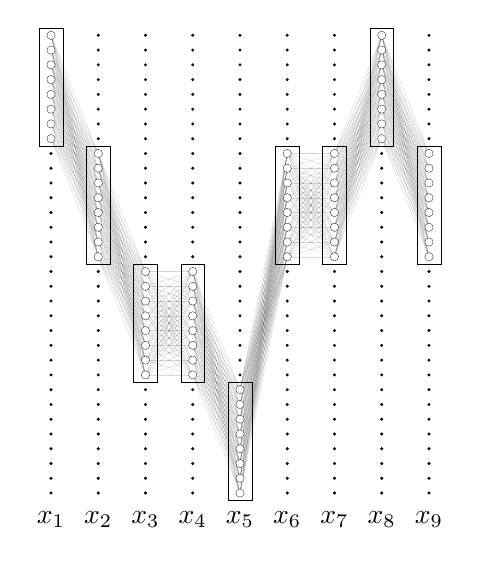
\begin{tikzpicture}%
\path[draw,line width=0.1pt,opacity=0.15,fill=black] (0.6,4.5) -- (1.2,3.0);%
\path[draw,line width=0.1pt,opacity=0.15,fill=black] (0.6,4.5) -- (1.2,3.1875);%
\path[draw,line width=0.1pt,opacity=0.15,fill=black] (0.6,4.5) -- (1.2,3.375);%
\path[draw,line width=0.1pt,opacity=0.15,fill=black] (0.6,4.5) -- (1.2,3.5625);%
\path[draw,line width=0.1pt,opacity=0.15,fill=black] (0.6,4.5) -- (1.2,3.75);%
\path[draw,line width=0.1pt,opacity=0.15,fill=black] (0.6,4.5) -- (1.2,3.9375);%
\path[draw,line width=0.1pt,opacity=0.15,fill=black] (0.6,4.5) -- (1.2,4.125);%
\path[draw,line width=0.1pt,opacity=0.15,fill=black] (0.6,4.5) -- (1.2,4.3125);%
\path[draw,line width=0.1pt,opacity=0.15,fill=black] (0.6,4.6875) -- (1.2,3.0);%
\path[draw,line width=0.1pt,opacity=0.15,fill=black] (0.6,4.6875) -- (1.2,3.1875);%
\path[draw,line width=0.1pt,opacity=0.15,fill=black] (0.6,4.6875) -- (1.2,3.375);%
\path[draw,line width=0.1pt,opacity=0.15,fill=black] (0.6,4.6875) -- (1.2,3.5625);%
\path[draw,line width=0.1pt,opacity=0.15,fill=black] (0.6,4.6875) -- (1.2,3.75);%
\path[draw,line width=0.1pt,opacity=0.15,fill=black] (0.6,4.6875) -- (1.2,3.9375);%
\path[draw,line width=0.1pt,opacity=0.15,fill=black] (0.6,4.6875) -- (1.2,4.125);%
\path[draw,line width=0.1pt,opacity=0.15,fill=black] (0.6,4.6875) -- (1.2,4.3125);%
\path[draw,line width=0.1pt,opacity=0.15,fill=black] (0.6,4.875) -- (1.2,3.0);%
\path[draw,line width=0.1pt,opacity=0.15,fill=black] (0.6,4.875) -- (1.2,3.1875);%
\path[draw,line width=0.1pt,opacity=0.15,fill=black] (0.6,4.875) -- (1.2,3.375);%
\path[draw,line width=0.1pt,opacity=0.15,fill=black] (0.6,4.875) -- (1.2,3.5625);%
\path[draw,line width=0.1pt,opacity=0.15,fill=black] (0.6,4.875) -- (1.2,3.75);%
\path[draw,line width=0.1pt,opacity=0.15,fill=black] (0.6,4.875) -- (1.2,3.9375);%
\path[draw,line width=0.1pt,opacity=0.15,fill=black] (0.6,4.875) -- (1.2,4.125);%
\path[draw,line width=0.1pt,opacity=0.15,fill=black] (0.6,4.875) -- (1.2,4.3125);%
\path[draw,line width=0.1pt,opacity=0.15,fill=black] (0.6,5.0625) -- (1.2,3.0);%
\path[draw,line width=0.1pt,opacity=0.15,fill=black] (0.6,5.0625) -- (1.2,3.1875);%
\path[draw,line width=0.1pt,opacity=0.15,fill=black] (0.6,5.0625) -- (1.2,3.375);%
\path[draw,line width=0.1pt,opacity=0.15,fill=black] (0.6,5.0625) -- (1.2,3.5625);%
\path[draw,line width=0.1pt,opacity=0.15,fill=black] (0.6,5.0625) -- (1.2,3.75);%
\path[draw,line width=0.1pt,opacity=0.15,fill=black] (0.6,5.0625) -- (1.2,3.9375);%
\path[draw,line width=0.1pt,opacity=0.15,fill=black] (0.6,5.0625) -- (1.2,4.125);%
\path[draw,line width=0.1pt,opacity=0.15,fill=black] (0.6,5.0625) -- (1.2,4.3125);%
\path[draw,line width=0.1pt,opacity=0.15,fill=black] (0.6,5.25) -- (1.2,3.0);%
\path[draw,line width=0.1pt,opacity=0.15,fill=black] (0.6,5.25) -- (1.2,3.1875);%
\path[draw,line width=0.1pt,opacity=0.15,fill=black] (0.6,5.25) -- (1.2,3.375);%
\path[draw,line width=0.1pt,opacity=0.15,fill=black] (0.6,5.25) -- (1.2,3.5625);%
\path[draw,line width=0.1pt,opacity=0.15,fill=black] (0.6,5.25) -- (1.2,3.75);%
\path[draw,line width=0.1pt,opacity=0.15,fill=black] (0.6,5.25) -- (1.2,3.9375);%
\path[draw,line width=0.1pt,opacity=0.15,fill=black] (0.6,5.25) -- (1.2,4.125);%
\path[draw,line width=0.1pt,opacity=0.15,fill=black] (0.6,5.25) -- (1.2,4.3125);%
\path[draw,line width=0.1pt,opacity=0.15,fill=black] (0.6,5.4375) -- (1.2,3.0);%
\path[draw,line width=0.1pt,opacity=0.15,fill=black] (0.6,5.4375) -- (1.2,3.1875);%
\path[draw,line width=0.1pt,opacity=0.15,fill=black] (0.6,5.4375) -- (1.2,3.375);%
\path[draw,line width=0.1pt,opacity=0.15,fill=black] (0.6,5.4375) -- (1.2,3.5625);%
\path[draw,line width=0.1pt,opacity=0.15,fill=black] (0.6,5.4375) -- (1.2,3.75);%
\path[draw,line width=0.1pt,opacity=0.15,fill=black] (0.6,5.4375) -- (1.2,3.9375);%
\path[draw,line width=0.1pt,opacity=0.15,fill=black] (0.6,5.4375) -- (1.2,4.125);%
\path[draw,line width=0.1pt,opacity=0.15,fill=black] (0.6,5.4375) -- (1.2,4.3125);%
\path[draw,line width=0.1pt,opacity=0.15,fill=black] (0.6,5.625) -- (1.2,3.0);%
\path[draw,line width=0.1pt,opacity=0.15,fill=black] (0.6,5.625) -- (1.2,3.1875);%
\path[draw,line width=0.1pt,opacity=0.15,fill=black] (0.6,5.625) -- (1.2,3.375);%
\path[draw,line width=0.1pt,opacity=0.15,fill=black] (0.6,5.625) -- (1.2,3.5625);%
\path[draw,line width=0.1pt,opacity=0.15,fill=black] (0.6,5.625) -- (1.2,3.75);%
\path[draw,line width=0.1pt,opacity=0.15,fill=black] (0.6,5.625) -- (1.2,3.9375);%
\path[draw,line width=0.1pt,opacity=0.15,fill=black] (0.6,5.625) -- (1.2,4.125);%
\path[draw,line width=0.1pt,opacity=0.15,fill=black] (0.6,5.625) -- (1.2,4.3125);%
\path[draw,line width=0.1pt,opacity=0.15,fill=black] (0.6,5.8125) -- (1.2,3.0);%
\path[draw,line width=0.1pt,opacity=0.15,fill=black] (0.6,5.8125) -- (1.2,3.1875);%
\path[draw,line width=0.1pt,opacity=0.15,fill=black] (0.6,5.8125) -- (1.2,3.375);%
\path[draw,line width=0.1pt,opacity=0.15,fill=black] (0.6,5.8125) -- (1.2,3.5625);%
\path[draw,line width=0.1pt,opacity=0.15,fill=black] (0.6,5.8125) -- (1.2,3.75);%
\path[draw,line width=0.1pt,opacity=0.15,fill=black] (0.6,5.8125) -- (1.2,3.9375);%
\path[draw,line width=0.1pt,opacity=0.15,fill=black] (0.6,5.8125) -- (1.2,4.125);%
\path[draw,line width=0.1pt,opacity=0.15,fill=black] (0.6,5.8125) -- (1.2,4.3125);%
\path[draw,line width=0.1pt,opacity=0.15,fill=black] (1.2,3.0) -- (1.8,1.5);%
\path[draw,line width=0.1pt,opacity=0.15,fill=black] (1.2,3.0) -- (1.8,1.6875);%
\path[draw,line width=0.1pt,opacity=0.15,fill=black] (1.2,3.0) -- (1.8,1.875);%
\path[draw,line width=0.1pt,opacity=0.15,fill=black] (1.2,3.0) -- (1.8,2.0625);%
\path[draw,line width=0.1pt,opacity=0.15,fill=black] (1.2,3.0) -- (1.8,2.25);%
\path[draw,line width=0.1pt,opacity=0.15,fill=black] (1.2,3.0) -- (1.8,2.4375);%
\path[draw,line width=0.1pt,opacity=0.15,fill=black] (1.2,3.0) -- (1.8,2.625);%
\path[draw,line width=0.1pt,opacity=0.15,fill=black] (1.2,3.0) -- (1.8,2.8125);%
\path[draw,line width=0.1pt,opacity=0.15,fill=black] (1.2,3.1875) -- (1.8,1.5);%
\path[draw,line width=0.1pt,opacity=0.15,fill=black] (1.2,3.1875) -- (1.8,1.6875);%
\path[draw,line width=0.1pt,opacity=0.15,fill=black] (1.2,3.1875) -- (1.8,1.875);%
\path[draw,line width=0.1pt,opacity=0.15,fill=black] (1.2,3.1875) -- (1.8,2.0625);%
\path[draw,line width=0.1pt,opacity=0.15,fill=black] (1.2,3.1875) -- (1.8,2.25);%
\path[draw,line width=0.1pt,opacity=0.15,fill=black] (1.2,3.1875) -- (1.8,2.4375);%
\path[draw,line width=0.1pt,opacity=0.15,fill=black] (1.2,3.1875) -- (1.8,2.625);%
\path[draw,line width=0.1pt,opacity=0.15,fill=black] (1.2,3.1875) -- (1.8,2.8125);%
\path[draw,line width=0.1pt,opacity=0.15,fill=black] (1.2,3.375) -- (1.8,1.5);%
\path[draw,line width=0.1pt,opacity=0.15,fill=black] (1.2,3.375) -- (1.8,1.6875);%
\path[draw,line width=0.1pt,opacity=0.15,fill=black] (1.2,3.375) -- (1.8,1.875);%
\path[draw,line width=0.1pt,opacity=0.15,fill=black] (1.2,3.375) -- (1.8,2.0625);%
\path[draw,line width=0.1pt,opacity=0.15,fill=black] (1.2,3.375) -- (1.8,2.25);%
\path[draw,line width=0.1pt,opacity=0.15,fill=black] (1.2,3.375) -- (1.8,2.4375);%
\path[draw,line width=0.1pt,opacity=0.15,fill=black] (1.2,3.375) -- (1.8,2.625);%
\path[draw,line width=0.1pt,opacity=0.15,fill=black] (1.2,3.375) -- (1.8,2.8125);%
\path[draw,line width=0.1pt,opacity=0.15,fill=black] (1.2,3.5625) -- (1.8,1.5);%
\path[draw,line width=0.1pt,opacity=0.15,fill=black] (1.2,3.5625) -- (1.8,1.6875);%
\path[draw,line width=0.1pt,opacity=0.15,fill=black] (1.2,3.5625) -- (1.8,1.875);%
\path[draw,line width=0.1pt,opacity=0.15,fill=black] (1.2,3.5625) -- (1.8,2.0625);%
\path[draw,line width=0.1pt,opacity=0.15,fill=black] (1.2,3.5625) -- (1.8,2.25);%
\path[draw,line width=0.1pt,opacity=0.15,fill=black] (1.2,3.5625) -- (1.8,2.4375);%
\path[draw,line width=0.1pt,opacity=0.15,fill=black] (1.2,3.5625) -- (1.8,2.625);%
\path[draw,line width=0.1pt,opacity=0.15,fill=black] (1.2,3.5625) -- (1.8,2.8125);%
\path[draw,line width=0.1pt,opacity=0.15,fill=black] (1.2,3.75) -- (1.8,1.5);%
\path[draw,line width=0.1pt,opacity=0.15,fill=black] (1.2,3.75) -- (1.8,1.6875);%
\path[draw,line width=0.1pt,opacity=0.15,fill=black] (1.2,3.75) -- (1.8,1.875);%
\path[draw,line width=0.1pt,opacity=0.15,fill=black] (1.2,3.75) -- (1.8,2.0625);%
\path[draw,line width=0.1pt,opacity=0.15,fill=black] (1.2,3.75) -- (1.8,2.25);%
\path[draw,line width=0.1pt,opacity=0.15,fill=black] (1.2,3.75) -- (1.8,2.4375);%
\path[draw,line width=0.1pt,opacity=0.15,fill=black] (1.2,3.75) -- (1.8,2.625);%
\path[draw,line width=0.1pt,opacity=0.15,fill=black] (1.2,3.75) -- (1.8,2.8125);%
\path[draw,line width=0.1pt,opacity=0.15,fill=black] (1.2,3.9375) -- (1.8,1.5);%
\path[draw,line width=0.1pt,opacity=0.15,fill=black] (1.2,3.9375) -- (1.8,1.6875);%
\path[draw,line width=0.1pt,opacity=0.15,fill=black] (1.2,3.9375) -- (1.8,1.875);%
\path[draw,line width=0.1pt,opacity=0.15,fill=black] (1.2,3.9375) -- (1.8,2.0625);%
\path[draw,line width=0.1pt,opacity=0.15,fill=black] (1.2,3.9375) -- (1.8,2.25);%
\path[draw,line width=0.1pt,opacity=0.15,fill=black] (1.2,3.9375) -- (1.8,2.4375);%
\path[draw,line width=0.1pt,opacity=0.15,fill=black] (1.2,3.9375) -- (1.8,2.625);%
\path[draw,line width=0.1pt,opacity=0.15,fill=black] (1.2,3.9375) -- (1.8,2.8125);%
\path[draw,line width=0.1pt,opacity=0.15,fill=black] (1.2,4.125) -- (1.8,1.5);%
\path[draw,line width=0.1pt,opacity=0.15,fill=black] (1.2,4.125) -- (1.8,1.6875);%
\path[draw,line width=0.1pt,opacity=0.15,fill=black] (1.2,4.125) -- (1.8,1.875);%
\path[draw,line width=0.1pt,opacity=0.15,fill=black] (1.2,4.125) -- (1.8,2.0625);%
\path[draw,line width=0.1pt,opacity=0.15,fill=black] (1.2,4.125) -- (1.8,2.25);%
\path[draw,line width=0.1pt,opacity=0.15,fill=black] (1.2,4.125) -- (1.8,2.4375);%
\path[draw,line width=0.1pt,opacity=0.15,fill=black] (1.2,4.125) -- (1.8,2.625);%
\path[draw,line width=0.1pt,opacity=0.15,fill=black] (1.2,4.125) -- (1.8,2.8125);%
\path[draw,line width=0.1pt,opacity=0.15,fill=black] (1.2,4.3125) -- (1.8,1.5);%
\path[draw,line width=0.1pt,opacity=0.15,fill=black] (1.2,4.3125) -- (1.8,1.6875);%
\path[draw,line width=0.1pt,opacity=0.15,fill=black] (1.2,4.3125) -- (1.8,1.875);%
\path[draw,line width=0.1pt,opacity=0.15,fill=black] (1.2,4.3125) -- (1.8,2.0625);%
\path[draw,line width=0.1pt,opacity=0.15,fill=black] (1.2,4.3125) -- (1.8,2.25);%
\path[draw,line width=0.1pt,opacity=0.15,fill=black] (1.2,4.3125) -- (1.8,2.4375);%
\path[draw,line width=0.1pt,opacity=0.15,fill=black] (1.2,4.3125) -- (1.8,2.625);%
\path[draw,line width=0.1pt,opacity=0.15,fill=black] (1.2,4.3125) -- (1.8,2.8125);%
\path[draw,line width=0.1pt,opacity=0.15,fill=black] (1.8,1.5) -- (2.4,1.5);%
\path[draw,line width=0.1pt,opacity=0.15,fill=black] (1.8,1.5) -- (2.4,1.6875);%
\path[draw,line width=0.1pt,opacity=0.15,fill=black] (1.8,1.5) -- (2.4,1.875);%
\path[draw,line width=0.1pt,opacity=0.15,fill=black] (1.8,1.5) -- (2.4,2.0625);%
\path[draw,line width=0.1pt,opacity=0.15,fill=black] (1.8,1.5) -- (2.4,2.25);%
\path[draw,line width=0.1pt,opacity=0.15,fill=black] (1.8,1.5) -- (2.4,2.4375);%
\path[draw,line width=0.1pt,opacity=0.15,fill=black] (1.8,1.5) -- (2.4,2.625);%
\path[draw,line width=0.1pt,opacity=0.15,fill=black] (1.8,1.5) -- (2.4,2.8125);%
\path[draw,line width=0.1pt,opacity=0.15,fill=black] (1.8,1.6875) -- (2.4,1.5);%
\path[draw,line width=0.1pt,opacity=0.15,fill=black] (1.8,1.6875) -- (2.4,1.6875);%
\path[draw,line width=0.1pt,opacity=0.15,fill=black] (1.8,1.6875) -- (2.4,1.875);%
\path[draw,line width=0.1pt,opacity=0.15,fill=black] (1.8,1.6875) -- (2.4,2.0625);%
\path[draw,line width=0.1pt,opacity=0.15,fill=black] (1.8,1.6875) -- (2.4,2.25);%
\path[draw,line width=0.1pt,opacity=0.15,fill=black] (1.8,1.6875) -- (2.4,2.4375);%
\path[draw,line width=0.1pt,opacity=0.15,fill=black] (1.8,1.6875) -- (2.4,2.625);%
\path[draw,line width=0.1pt,opacity=0.15,fill=black] (1.8,1.6875) -- (2.4,2.8125);%
\path[draw,line width=0.1pt,opacity=0.15,fill=black] (1.8,1.875) -- (2.4,1.5);%
\path[draw,line width=0.1pt,opacity=0.15,fill=black] (1.8,1.875) -- (2.4,1.6875);%
\path[draw,line width=0.1pt,opacity=0.15,fill=black] (1.8,1.875) -- (2.4,1.875);%
\path[draw,line width=0.1pt,opacity=0.15,fill=black] (1.8,1.875) -- (2.4,2.0625);%
\path[draw,line width=0.1pt,opacity=0.15,fill=black] (1.8,1.875) -- (2.4,2.25);%
\path[draw,line width=0.1pt,opacity=0.15,fill=black] (1.8,1.875) -- (2.4,2.4375);%
\path[draw,line width=0.1pt,opacity=0.15,fill=black] (1.8,1.875) -- (2.4,2.625);%
\path[draw,line width=0.1pt,opacity=0.15,fill=black] (1.8,1.875) -- (2.4,2.8125);%
\path[draw,line width=0.1pt,opacity=0.15,fill=black] (1.8,2.0625) -- (2.4,1.5);%
\path[draw,line width=0.1pt,opacity=0.15,fill=black] (1.8,2.0625) -- (2.4,1.6875);%
\path[draw,line width=0.1pt,opacity=0.15,fill=black] (1.8,2.0625) -- (2.4,1.875);%
\path[draw,line width=0.1pt,opacity=0.15,fill=black] (1.8,2.0625) -- (2.4,2.0625);%
\path[draw,line width=0.1pt,opacity=0.15,fill=black] (1.8,2.0625) -- (2.4,2.25);%
\path[draw,line width=0.1pt,opacity=0.15,fill=black] (1.8,2.0625) -- (2.4,2.4375);%
\path[draw,line width=0.1pt,opacity=0.15,fill=black] (1.8,2.0625) -- (2.4,2.625);%
\path[draw,line width=0.1pt,opacity=0.15,fill=black] (1.8,2.0625) -- (2.4,2.8125);%
\path[draw,line width=0.1pt,opacity=0.15,fill=black] (1.8,2.25) -- (2.4,1.5);%
\path[draw,line width=0.1pt,opacity=0.15,fill=black] (1.8,2.25) -- (2.4,1.6875);%
\path[draw,line width=0.1pt,opacity=0.15,fill=black] (1.8,2.25) -- (2.4,1.875);%
\path[draw,line width=0.1pt,opacity=0.15,fill=black] (1.8,2.25) -- (2.4,2.0625);%
\path[draw,line width=0.1pt,opacity=0.15,fill=black] (1.8,2.25) -- (2.4,2.25);%
\path[draw,line width=0.1pt,opacity=0.15,fill=black] (1.8,2.25) -- (2.4,2.4375);%
\path[draw,line width=0.1pt,opacity=0.15,fill=black] (1.8,2.25) -- (2.4,2.625);%
\path[draw,line width=0.1pt,opacity=0.15,fill=black] (1.8,2.25) -- (2.4,2.8125);%
\path[draw,line width=0.1pt,opacity=0.15,fill=black] (1.8,2.4375) -- (2.4,1.5);%
\path[draw,line width=0.1pt,opacity=0.15,fill=black] (1.8,2.4375) -- (2.4,1.6875);%
\path[draw,line width=0.1pt,opacity=0.15,fill=black] (1.8,2.4375) -- (2.4,1.875);%
\path[draw,line width=0.1pt,opacity=0.15,fill=black] (1.8,2.4375) -- (2.4,2.0625);%
\path[draw,line width=0.1pt,opacity=0.15,fill=black] (1.8,2.4375) -- (2.4,2.25);%
\path[draw,line width=0.1pt,opacity=0.15,fill=black] (1.8,2.4375) -- (2.4,2.4375);%
\path[draw,line width=0.1pt,opacity=0.15,fill=black] (1.8,2.4375) -- (2.4,2.625);%
\path[draw,line width=0.1pt,opacity=0.15,fill=black] (1.8,2.4375) -- (2.4,2.8125);%
\path[draw,line width=0.1pt,opacity=0.15,fill=black] (1.8,2.625) -- (2.4,1.5);%
\path[draw,line width=0.1pt,opacity=0.15,fill=black] (1.8,2.625) -- (2.4,1.6875);%
\path[draw,line width=0.1pt,opacity=0.15,fill=black] (1.8,2.625) -- (2.4,1.875);%
\path[draw,line width=0.1pt,opacity=0.15,fill=black] (1.8,2.625) -- (2.4,2.0625);%
\path[draw,line width=0.1pt,opacity=0.15,fill=black] (1.8,2.625) -- (2.4,2.25);%
\path[draw,line width=0.1pt,opacity=0.15,fill=black] (1.8,2.625) -- (2.4,2.4375);%
\path[draw,line width=0.1pt,opacity=0.15,fill=black] (1.8,2.625) -- (2.4,2.625);%
\path[draw,line width=0.1pt,opacity=0.15,fill=black] (1.8,2.625) -- (2.4,2.8125);%
\path[draw,line width=0.1pt,opacity=0.15,fill=black] (1.8,2.8125) -- (2.4,1.5);%
\path[draw,line width=0.1pt,opacity=0.15,fill=black] (1.8,2.8125) -- (2.4,1.6875);%
\path[draw,line width=0.1pt,opacity=0.15,fill=black] (1.8,2.8125) -- (2.4,1.875);%
\path[draw,line width=0.1pt,opacity=0.15,fill=black] (1.8,2.8125) -- (2.4,2.0625);%
\path[draw,line width=0.1pt,opacity=0.15,fill=black] (1.8,2.8125) -- (2.4,2.25);%
\path[draw,line width=0.1pt,opacity=0.15,fill=black] (1.8,2.8125) -- (2.4,2.4375);%
\path[draw,line width=0.1pt,opacity=0.15,fill=black] (1.8,2.8125) -- (2.4,2.625);%
\path[draw,line width=0.1pt,opacity=0.15,fill=black] (1.8,2.8125) -- (2.4,2.8125);%
\path[draw,line width=0.1pt,opacity=0.15,fill=black] (2.4,1.5) -- (3.0,0.0);%
\path[draw,line width=0.1pt,opacity=0.15,fill=black] (2.4,1.5) -- (3.0,0.1875);%
\path[draw,line width=0.1pt,opacity=0.15,fill=black] (2.4,1.5) -- (3.0,0.375);%
\path[draw,line width=0.1pt,opacity=0.15,fill=black] (2.4,1.5) -- (3.0,0.5625);%
\path[draw,line width=0.1pt,opacity=0.15,fill=black] (2.4,1.5) -- (3.0,0.75);%
\path[draw,line width=0.1pt,opacity=0.15,fill=black] (2.4,1.5) -- (3.0,0.9375);%
\path[draw,line width=0.1pt,opacity=0.15,fill=black] (2.4,1.5) -- (3.0,1.125);%
\path[draw,line width=0.1pt,opacity=0.15,fill=black] (2.4,1.5) -- (3.0,1.3125);%
\path[draw,line width=0.1pt,opacity=0.15,fill=black] (2.4,1.6875) -- (3.0,0.0);%
\path[draw,line width=0.1pt,opacity=0.15,fill=black] (2.4,1.6875) -- (3.0,0.1875);%
\path[draw,line width=0.1pt,opacity=0.15,fill=black] (2.4,1.6875) -- (3.0,0.375);%
\path[draw,line width=0.1pt,opacity=0.15,fill=black] (2.4,1.6875) -- (3.0,0.5625);%
\path[draw,line width=0.1pt,opacity=0.15,fill=black] (2.4,1.6875) -- (3.0,0.75);%
\path[draw,line width=0.1pt,opacity=0.15,fill=black] (2.4,1.6875) -- (3.0,0.9375);%
\path[draw,line width=0.1pt,opacity=0.15,fill=black] (2.4,1.6875) -- (3.0,1.125);%
\path[draw,line width=0.1pt,opacity=0.15,fill=black] (2.4,1.6875) -- (3.0,1.3125);%
\path[draw,line width=0.1pt,opacity=0.15,fill=black] (2.4,1.875) -- (3.0,0.0);%
\path[draw,line width=0.1pt,opacity=0.15,fill=black] (2.4,1.875) -- (3.0,0.1875);%
\path[draw,line width=0.1pt,opacity=0.15,fill=black] (2.4,1.875) -- (3.0,0.375);%
\path[draw,line width=0.1pt,opacity=0.15,fill=black] (2.4,1.875) -- (3.0,0.5625);%
\path[draw,line width=0.1pt,opacity=0.15,fill=black] (2.4,1.875) -- (3.0,0.75);%
\path[draw,line width=0.1pt,opacity=0.15,fill=black] (2.4,1.875) -- (3.0,0.9375);%
\path[draw,line width=0.1pt,opacity=0.15,fill=black] (2.4,1.875) -- (3.0,1.125);%
\path[draw,line width=0.1pt,opacity=0.15,fill=black] (2.4,1.875) -- (3.0,1.3125);%
\path[draw,line width=0.1pt,opacity=0.15,fill=black] (2.4,2.0625) -- (3.0,0.0);%
\path[draw,line width=0.1pt,opacity=0.15,fill=black] (2.4,2.0625) -- (3.0,0.1875);%
\path[draw,line width=0.1pt,opacity=0.15,fill=black] (2.4,2.0625) -- (3.0,0.375);%
\path[draw,line width=0.1pt,opacity=0.15,fill=black] (2.4,2.0625) -- (3.0,0.5625);%
\path[draw,line width=0.1pt,opacity=0.15,fill=black] (2.4,2.0625) -- (3.0,0.75);%
\path[draw,line width=0.1pt,opacity=0.15,fill=black] (2.4,2.0625) -- (3.0,0.9375);%
\path[draw,line width=0.1pt,opacity=0.15,fill=black] (2.4,2.0625) -- (3.0,1.125);%
\path[draw,line width=0.1pt,opacity=0.15,fill=black] (2.4,2.0625) -- (3.0,1.3125);%
\path[draw,line width=0.1pt,opacity=0.15,fill=black] (2.4,2.25) -- (3.0,0.0);%
\path[draw,line width=0.1pt,opacity=0.15,fill=black] (2.4,2.25) -- (3.0,0.1875);%
\path[draw,line width=0.1pt,opacity=0.15,fill=black] (2.4,2.25) -- (3.0,0.375);%
\path[draw,line width=0.1pt,opacity=0.15,fill=black] (2.4,2.25) -- (3.0,0.5625);%
\path[draw,line width=0.1pt,opacity=0.15,fill=black] (2.4,2.25) -- (3.0,0.75);%
\path[draw,line width=0.1pt,opacity=0.15,fill=black] (2.4,2.25) -- (3.0,0.9375);%
\path[draw,line width=0.1pt,opacity=0.15,fill=black] (2.4,2.25) -- (3.0,1.125);%
\path[draw,line width=0.1pt,opacity=0.15,fill=black] (2.4,2.25) -- (3.0,1.3125);%
\path[draw,line width=0.1pt,opacity=0.15,fill=black] (2.4,2.4375) -- (3.0,0.0);%
\path[draw,line width=0.1pt,opacity=0.15,fill=black] (2.4,2.4375) -- (3.0,0.1875);%
\path[draw,line width=0.1pt,opacity=0.15,fill=black] (2.4,2.4375) -- (3.0,0.375);%
\path[draw,line width=0.1pt,opacity=0.15,fill=black] (2.4,2.4375) -- (3.0,0.5625);%
\path[draw,line width=0.1pt,opacity=0.15,fill=black] (2.4,2.4375) -- (3.0,0.75);%
\path[draw,line width=0.1pt,opacity=0.15,fill=black] (2.4,2.4375) -- (3.0,0.9375);%
\path[draw,line width=0.1pt,opacity=0.15,fill=black] (2.4,2.4375) -- (3.0,1.125);%
\path[draw,line width=0.1pt,opacity=0.15,fill=black] (2.4,2.4375) -- (3.0,1.3125);%
\path[draw,line width=0.1pt,opacity=0.15,fill=black] (2.4,2.625) -- (3.0,0.0);%
\path[draw,line width=0.1pt,opacity=0.15,fill=black] (2.4,2.625) -- (3.0,0.1875);%
\path[draw,line width=0.1pt,opacity=0.15,fill=black] (2.4,2.625) -- (3.0,0.375);%
\path[draw,line width=0.1pt,opacity=0.15,fill=black] (2.4,2.625) -- (3.0,0.5625);%
\path[draw,line width=0.1pt,opacity=0.15,fill=black] (2.4,2.625) -- (3.0,0.75);%
\path[draw,line width=0.1pt,opacity=0.15,fill=black] (2.4,2.625) -- (3.0,0.9375);%
\path[draw,line width=0.1pt,opacity=0.15,fill=black] (2.4,2.625) -- (3.0,1.125);%
\path[draw,line width=0.1pt,opacity=0.15,fill=black] (2.4,2.625) -- (3.0,1.3125);%
\path[draw,line width=0.1pt,opacity=0.15,fill=black] (2.4,2.8125) -- (3.0,0.0);%
\path[draw,line width=0.1pt,opacity=0.15,fill=black] (2.4,2.8125) -- (3.0,0.1875);%
\path[draw,line width=0.1pt,opacity=0.15,fill=black] (2.4,2.8125) -- (3.0,0.375);%
\path[draw,line width=0.1pt,opacity=0.15,fill=black] (2.4,2.8125) -- (3.0,0.5625);%
\path[draw,line width=0.1pt,opacity=0.15,fill=black] (2.4,2.8125) -- (3.0,0.75);%
\path[draw,line width=0.1pt,opacity=0.15,fill=black] (2.4,2.8125) -- (3.0,0.9375);%
\path[draw,line width=0.1pt,opacity=0.15,fill=black] (2.4,2.8125) -- (3.0,1.125);%
\path[draw,line width=0.1pt,opacity=0.15,fill=black] (2.4,2.8125) -- (3.0,1.3125);%
\path[draw,line width=0.1pt,opacity=0.15,fill=black] (3.0,0.0) -- (3.6,3.0);%
\path[draw,line width=0.1pt,opacity=0.15,fill=black] (3.0,0.0) -- (3.6,3.1875);%
\path[draw,line width=0.1pt,opacity=0.15,fill=black] (3.0,0.0) -- (3.6,3.375);%
\path[draw,line width=0.1pt,opacity=0.15,fill=black] (3.0,0.0) -- (3.6,3.5625);%
\path[draw,line width=0.1pt,opacity=0.15,fill=black] (3.0,0.0) -- (3.6,3.75);%
\path[draw,line width=0.1pt,opacity=0.15,fill=black] (3.0,0.0) -- (3.6,3.9375);%
\path[draw,line width=0.1pt,opacity=0.15,fill=black] (3.0,0.0) -- (3.6,4.125);%
\path[draw,line width=0.1pt,opacity=0.15,fill=black] (3.0,0.0) -- (3.6,4.3125);%
\path[draw,line width=0.1pt,opacity=0.15,fill=black] (3.0,0.1875) -- (3.6,3.0);%
\path[draw,line width=0.1pt,opacity=0.15,fill=black] (3.0,0.1875) -- (3.6,3.1875);%
\path[draw,line width=0.1pt,opacity=0.15,fill=black] (3.0,0.1875) -- (3.6,3.375);%
\path[draw,line width=0.1pt,opacity=0.15,fill=black] (3.0,0.1875) -- (3.6,3.5625);%
\path[draw,line width=0.1pt,opacity=0.15,fill=black] (3.0,0.1875) -- (3.6,3.75);%
\path[draw,line width=0.1pt,opacity=0.15,fill=black] (3.0,0.1875) -- (3.6,3.9375);%
\path[draw,line width=0.1pt,opacity=0.15,fill=black] (3.0,0.1875) -- (3.6,4.125);%
\path[draw,line width=0.1pt,opacity=0.15,fill=black] (3.0,0.1875) -- (3.6,4.3125);%
\path[draw,line width=0.1pt,opacity=0.15,fill=black] (3.0,0.375) -- (3.6,3.0);%
\path[draw,line width=0.1pt,opacity=0.15,fill=black] (3.0,0.375) -- (3.6,3.1875);%
\path[draw,line width=0.1pt,opacity=0.15,fill=black] (3.0,0.375) -- (3.6,3.375);%
\path[draw,line width=0.1pt,opacity=0.15,fill=black] (3.0,0.375) -- (3.6,3.5625);%
\path[draw,line width=0.1pt,opacity=0.15,fill=black] (3.0,0.375) -- (3.6,3.75);%
\path[draw,line width=0.1pt,opacity=0.15,fill=black] (3.0,0.375) -- (3.6,3.9375);%
\path[draw,line width=0.1pt,opacity=0.15,fill=black] (3.0,0.375) -- (3.6,4.125);%
\path[draw,line width=0.1pt,opacity=0.15,fill=black] (3.0,0.375) -- (3.6,4.3125);%
\path[draw,line width=0.1pt,opacity=0.15,fill=black] (3.0,0.5625) -- (3.6,3.0);%
\path[draw,line width=0.1pt,opacity=0.15,fill=black] (3.0,0.5625) -- (3.6,3.1875);%
\path[draw,line width=0.1pt,opacity=0.15,fill=black] (3.0,0.5625) -- (3.6,3.375);%
\path[draw,line width=0.1pt,opacity=0.15,fill=black] (3.0,0.5625) -- (3.6,3.5625);%
\path[draw,line width=0.1pt,opacity=0.15,fill=black] (3.0,0.5625) -- (3.6,3.75);%
\path[draw,line width=0.1pt,opacity=0.15,fill=black] (3.0,0.5625) -- (3.6,3.9375);%
\path[draw,line width=0.1pt,opacity=0.15,fill=black] (3.0,0.5625) -- (3.6,4.125);%
\path[draw,line width=0.1pt,opacity=0.15,fill=black] (3.0,0.5625) -- (3.6,4.3125);%
\path[draw,line width=0.1pt,opacity=0.15,fill=black] (3.0,0.75) -- (3.6,3.0);%
\path[draw,line width=0.1pt,opacity=0.15,fill=black] (3.0,0.75) -- (3.6,3.1875);%
\path[draw,line width=0.1pt,opacity=0.15,fill=black] (3.0,0.75) -- (3.6,3.375);%
\path[draw,line width=0.1pt,opacity=0.15,fill=black] (3.0,0.75) -- (3.6,3.5625);%
\path[draw,line width=0.1pt,opacity=0.15,fill=black] (3.0,0.75) -- (3.6,3.75);%
\path[draw,line width=0.1pt,opacity=0.15,fill=black] (3.0,0.75) -- (3.6,3.9375);%
\path[draw,line width=0.1pt,opacity=0.15,fill=black] (3.0,0.75) -- (3.6,4.125);%
\path[draw,line width=0.1pt,opacity=0.15,fill=black] (3.0,0.75) -- (3.6,4.3125);%
\path[draw,line width=0.1pt,opacity=0.15,fill=black] (3.0,0.9375) -- (3.6,3.0);%
\path[draw,line width=0.1pt,opacity=0.15,fill=black] (3.0,0.9375) -- (3.6,3.1875);%
\path[draw,line width=0.1pt,opacity=0.15,fill=black] (3.0,0.9375) -- (3.6,3.375);%
\path[draw,line width=0.1pt,opacity=0.15,fill=black] (3.0,0.9375) -- (3.6,3.5625);%
\path[draw,line width=0.1pt,opacity=0.15,fill=black] (3.0,0.9375) -- (3.6,3.75);%
\path[draw,line width=0.1pt,opacity=0.15,fill=black] (3.0,0.9375) -- (3.6,3.9375);%
\path[draw,line width=0.1pt,opacity=0.15,fill=black] (3.0,0.9375) -- (3.6,4.125);%
\path[draw,line width=0.1pt,opacity=0.15,fill=black] (3.0,0.9375) -- (3.6,4.3125);%
\path[draw,line width=0.1pt,opacity=0.15,fill=black] (3.0,1.125) -- (3.6,3.0);%
\path[draw,line width=0.1pt,opacity=0.15,fill=black] (3.0,1.125) -- (3.6,3.1875);%
\path[draw,line width=0.1pt,opacity=0.15,fill=black] (3.0,1.125) -- (3.6,3.375);%
\path[draw,line width=0.1pt,opacity=0.15,fill=black] (3.0,1.125) -- (3.6,3.5625);%
\path[draw,line width=0.1pt,opacity=0.15,fill=black] (3.0,1.125) -- (3.6,3.75);%
\path[draw,line width=0.1pt,opacity=0.15,fill=black] (3.0,1.125) -- (3.6,3.9375);%
\path[draw,line width=0.1pt,opacity=0.15,fill=black] (3.0,1.125) -- (3.6,4.125);%
\path[draw,line width=0.1pt,opacity=0.15,fill=black] (3.0,1.125) -- (3.6,4.3125);%
\path[draw,line width=0.1pt,opacity=0.15,fill=black] (3.0,1.3125) -- (3.6,3.0);%
\path[draw,line width=0.1pt,opacity=0.15,fill=black] (3.0,1.3125) -- (3.6,3.1875);%
\path[draw,line width=0.1pt,opacity=0.15,fill=black] (3.0,1.3125) -- (3.6,3.375);%
\path[draw,line width=0.1pt,opacity=0.15,fill=black] (3.0,1.3125) -- (3.6,3.5625);%
\path[draw,line width=0.1pt,opacity=0.15,fill=black] (3.0,1.3125) -- (3.6,3.75);%
\path[draw,line width=0.1pt,opacity=0.15,fill=black] (3.0,1.3125) -- (3.6,3.9375);%
\path[draw,line width=0.1pt,opacity=0.15,fill=black] (3.0,1.3125) -- (3.6,4.125);%
\path[draw,line width=0.1pt,opacity=0.15,fill=black] (3.0,1.3125) -- (3.6,4.3125);%
\path[draw,line width=0.1pt,opacity=0.15,fill=black] (3.6,3.0) -- (4.2,3.0);%
\path[draw,line width=0.1pt,opacity=0.15,fill=black] (3.6,3.0) -- (4.2,3.1875);%
\path[draw,line width=0.1pt,opacity=0.15,fill=black] (3.6,3.0) -- (4.2,3.375);%
\path[draw,line width=0.1pt,opacity=0.15,fill=black] (3.6,3.0) -- (4.2,3.5625);%
\path[draw,line width=0.1pt,opacity=0.15,fill=black] (3.6,3.0) -- (4.2,3.75);%
\path[draw,line width=0.1pt,opacity=0.15,fill=black] (3.6,3.0) -- (4.2,3.9375);%
\path[draw,line width=0.1pt,opacity=0.15,fill=black] (3.6,3.0) -- (4.2,4.125);%
\path[draw,line width=0.1pt,opacity=0.15,fill=black] (3.6,3.0) -- (4.2,4.3125);%
\path[draw,line width=0.1pt,opacity=0.15,fill=black] (3.6,3.1875) -- (4.2,3.0);%
\path[draw,line width=0.1pt,opacity=0.15,fill=black] (3.6,3.1875) -- (4.2,3.1875);%
\path[draw,line width=0.1pt,opacity=0.15,fill=black] (3.6,3.1875) -- (4.2,3.375);%
\path[draw,line width=0.1pt,opacity=0.15,fill=black] (3.6,3.1875) -- (4.2,3.5625);%
\path[draw,line width=0.1pt,opacity=0.15,fill=black] (3.6,3.1875) -- (4.2,3.75);%
\path[draw,line width=0.1pt,opacity=0.15,fill=black] (3.6,3.1875) -- (4.2,3.9375);%
\path[draw,line width=0.1pt,opacity=0.15,fill=black] (3.6,3.1875) -- (4.2,4.125);%
\path[draw,line width=0.1pt,opacity=0.15,fill=black] (3.6,3.1875) -- (4.2,4.3125);%
\path[draw,line width=0.1pt,opacity=0.15,fill=black] (3.6,3.375) -- (4.2,3.0);%
\path[draw,line width=0.1pt,opacity=0.15,fill=black] (3.6,3.375) -- (4.2,3.1875);%
\path[draw,line width=0.1pt,opacity=0.15,fill=black] (3.6,3.375) -- (4.2,3.375);%
\path[draw,line width=0.1pt,opacity=0.15,fill=black] (3.6,3.375) -- (4.2,3.5625);%
\path[draw,line width=0.1pt,opacity=0.15,fill=black] (3.6,3.375) -- (4.2,3.75);%
\path[draw,line width=0.1pt,opacity=0.15,fill=black] (3.6,3.375) -- (4.2,3.9375);%
\path[draw,line width=0.1pt,opacity=0.15,fill=black] (3.6,3.375) -- (4.2,4.125);%
\path[draw,line width=0.1pt,opacity=0.15,fill=black] (3.6,3.375) -- (4.2,4.3125);%
\path[draw,line width=0.1pt,opacity=0.15,fill=black] (3.6,3.5625) -- (4.2,3.0);%
\path[draw,line width=0.1pt,opacity=0.15,fill=black] (3.6,3.5625) -- (4.2,3.1875);%
\path[draw,line width=0.1pt,opacity=0.15,fill=black] (3.6,3.5625) -- (4.2,3.375);%
\path[draw,line width=0.1pt,opacity=0.15,fill=black] (3.6,3.5625) -- (4.2,3.5625);%
\path[draw,line width=0.1pt,opacity=0.15,fill=black] (3.6,3.5625) -- (4.2,3.75);%
\path[draw,line width=0.1pt,opacity=0.15,fill=black] (3.6,3.5625) -- (4.2,3.9375);%
\path[draw,line width=0.1pt,opacity=0.15,fill=black] (3.6,3.5625) -- (4.2,4.125);%
\path[draw,line width=0.1pt,opacity=0.15,fill=black] (3.6,3.5625) -- (4.2,4.3125);%
\path[draw,line width=0.1pt,opacity=0.15,fill=black] (3.6,3.75) -- (4.2,3.0);%
\path[draw,line width=0.1pt,opacity=0.15,fill=black] (3.6,3.75) -- (4.2,3.1875);%
\path[draw,line width=0.1pt,opacity=0.15,fill=black] (3.6,3.75) -- (4.2,3.375);%
\path[draw,line width=0.1pt,opacity=0.15,fill=black] (3.6,3.75) -- (4.2,3.5625);%
\path[draw,line width=0.1pt,opacity=0.15,fill=black] (3.6,3.75) -- (4.2,3.75);%
\path[draw,line width=0.1pt,opacity=0.15,fill=black] (3.6,3.75) -- (4.2,3.9375);%
\path[draw,line width=0.1pt,opacity=0.15,fill=black] (3.6,3.75) -- (4.2,4.125);%
\path[draw,line width=0.1pt,opacity=0.15,fill=black] (3.6,3.75) -- (4.2,4.3125);%
\path[draw,line width=0.1pt,opacity=0.15,fill=black] (3.6,3.9375) -- (4.2,3.0);%
\path[draw,line width=0.1pt,opacity=0.15,fill=black] (3.6,3.9375) -- (4.2,3.1875);%
\path[draw,line width=0.1pt,opacity=0.15,fill=black] (3.6,3.9375) -- (4.2,3.375);%
\path[draw,line width=0.1pt,opacity=0.15,fill=black] (3.6,3.9375) -- (4.2,3.5625);%
\path[draw,line width=0.1pt,opacity=0.15,fill=black] (3.6,3.9375) -- (4.2,3.75);%
\path[draw,line width=0.1pt,opacity=0.15,fill=black] (3.6,3.9375) -- (4.2,3.9375);%
\path[draw,line width=0.1pt,opacity=0.15,fill=black] (3.6,3.9375) -- (4.2,4.125);%
\path[draw,line width=0.1pt,opacity=0.15,fill=black] (3.6,3.9375) -- (4.2,4.3125);%
\path[draw,line width=0.1pt,opacity=0.15,fill=black] (3.6,4.125) -- (4.2,3.0);%
\path[draw,line width=0.1pt,opacity=0.15,fill=black] (3.6,4.125) -- (4.2,3.1875);%
\path[draw,line width=0.1pt,opacity=0.15,fill=black] (3.6,4.125) -- (4.2,3.375);%
\path[draw,line width=0.1pt,opacity=0.15,fill=black] (3.6,4.125) -- (4.2,3.5625);%
\path[draw,line width=0.1pt,opacity=0.15,fill=black] (3.6,4.125) -- (4.2,3.75);%
\path[draw,line width=0.1pt,opacity=0.15,fill=black] (3.6,4.125) -- (4.2,3.9375);%
\path[draw,line width=0.1pt,opacity=0.15,fill=black] (3.6,4.125) -- (4.2,4.125);%
\path[draw,line width=0.1pt,opacity=0.15,fill=black] (3.6,4.125) -- (4.2,4.3125);%
\path[draw,line width=0.1pt,opacity=0.15,fill=black] (3.6,4.3125) -- (4.2,3.0);%
\path[draw,line width=0.1pt,opacity=0.15,fill=black] (3.6,4.3125) -- (4.2,3.1875);%
\path[draw,line width=0.1pt,opacity=0.15,fill=black] (3.6,4.3125) -- (4.2,3.375);%
\path[draw,line width=0.1pt,opacity=0.15,fill=black] (3.6,4.3125) -- (4.2,3.5625);%
\path[draw,line width=0.1pt,opacity=0.15,fill=black] (3.6,4.3125) -- (4.2,3.75);%
\path[draw,line width=0.1pt,opacity=0.15,fill=black] (3.6,4.3125) -- (4.2,3.9375);%
\path[draw,line width=0.1pt,opacity=0.15,fill=black] (3.6,4.3125) -- (4.2,4.125);%
\path[draw,line width=0.1pt,opacity=0.15,fill=black] (3.6,4.3125) -- (4.2,4.3125);%
\path[draw,line width=0.1pt,opacity=0.15,fill=black] (4.2,3.0) -- (4.8,4.5);%
\path[draw,line width=0.1pt,opacity=0.15,fill=black] (4.2,3.0) -- (4.8,4.6875);%
\path[draw,line width=0.1pt,opacity=0.15,fill=black] (4.2,3.0) -- (4.8,4.875);%
\path[draw,line width=0.1pt,opacity=0.15,fill=black] (4.2,3.0) -- (4.8,5.0625);%
\path[draw,line width=0.1pt,opacity=0.15,fill=black] (4.2,3.0) -- (4.8,5.25);%
\path[draw,line width=0.1pt,opacity=0.15,fill=black] (4.2,3.0) -- (4.8,5.4375);%
\path[draw,line width=0.1pt,opacity=0.15,fill=black] (4.2,3.0) -- (4.8,5.625);%
\path[draw,line width=0.1pt,opacity=0.15,fill=black] (4.2,3.0) -- (4.8,5.8125);%
\path[draw,line width=0.1pt,opacity=0.15,fill=black] (4.2,3.1875) -- (4.8,4.5);%
\path[draw,line width=0.1pt,opacity=0.15,fill=black] (4.2,3.1875) -- (4.8,4.6875);%
\path[draw,line width=0.1pt,opacity=0.15,fill=black] (4.2,3.1875) -- (4.8,4.875);%
\path[draw,line width=0.1pt,opacity=0.15,fill=black] (4.2,3.1875) -- (4.8,5.0625);%
\path[draw,line width=0.1pt,opacity=0.15,fill=black] (4.2,3.1875) -- (4.8,5.25);%
\path[draw,line width=0.1pt,opacity=0.15,fill=black] (4.2,3.1875) -- (4.8,5.4375);%
\path[draw,line width=0.1pt,opacity=0.15,fill=black] (4.2,3.1875) -- (4.8,5.625);%
\path[draw,line width=0.1pt,opacity=0.15,fill=black] (4.2,3.1875) -- (4.8,5.8125);%
\path[draw,line width=0.1pt,opacity=0.15,fill=black] (4.2,3.375) -- (4.8,4.5);%
\path[draw,line width=0.1pt,opacity=0.15,fill=black] (4.2,3.375) -- (4.8,4.6875);%
\path[draw,line width=0.1pt,opacity=0.15,fill=black] (4.2,3.375) -- (4.8,4.875);%
\path[draw,line width=0.1pt,opacity=0.15,fill=black] (4.2,3.375) -- (4.8,5.0625);%
\path[draw,line width=0.1pt,opacity=0.15,fill=black] (4.2,3.375) -- (4.8,5.25);%
\path[draw,line width=0.1pt,opacity=0.15,fill=black] (4.2,3.375) -- (4.8,5.4375);%
\path[draw,line width=0.1pt,opacity=0.15,fill=black] (4.2,3.375) -- (4.8,5.625);%
\path[draw,line width=0.1pt,opacity=0.15,fill=black] (4.2,3.375) -- (4.8,5.8125);%
\path[draw,line width=0.1pt,opacity=0.15,fill=black] (4.2,3.5625) -- (4.8,4.5);%
\path[draw,line width=0.1pt,opacity=0.15,fill=black] (4.2,3.5625) -- (4.8,4.6875);%
\path[draw,line width=0.1pt,opacity=0.15,fill=black] (4.2,3.5625) -- (4.8,4.875);%
\path[draw,line width=0.1pt,opacity=0.15,fill=black] (4.2,3.5625) -- (4.8,5.0625);%
\path[draw,line width=0.1pt,opacity=0.15,fill=black] (4.2,3.5625) -- (4.8,5.25);%
\path[draw,line width=0.1pt,opacity=0.15,fill=black] (4.2,3.5625) -- (4.8,5.4375);%
\path[draw,line width=0.1pt,opacity=0.15,fill=black] (4.2,3.5625) -- (4.8,5.625);%
\path[draw,line width=0.1pt,opacity=0.15,fill=black] (4.2,3.5625) -- (4.8,5.8125);%
\path[draw,line width=0.1pt,opacity=0.15,fill=black] (4.2,3.75) -- (4.8,4.5);%
\path[draw,line width=0.1pt,opacity=0.15,fill=black] (4.2,3.75) -- (4.8,4.6875);%
\path[draw,line width=0.1pt,opacity=0.15,fill=black] (4.2,3.75) -- (4.8,4.875);%
\path[draw,line width=0.1pt,opacity=0.15,fill=black] (4.2,3.75) -- (4.8,5.0625);%
\path[draw,line width=0.1pt,opacity=0.15,fill=black] (4.2,3.75) -- (4.8,5.25);%
\path[draw,line width=0.1pt,opacity=0.15,fill=black] (4.2,3.75) -- (4.8,5.4375);%
\path[draw,line width=0.1pt,opacity=0.15,fill=black] (4.2,3.75) -- (4.8,5.625);%
\path[draw,line width=0.1pt,opacity=0.15,fill=black] (4.2,3.75) -- (4.8,5.8125);%
\path[draw,line width=0.1pt,opacity=0.15,fill=black] (4.2,3.9375) -- (4.8,4.5);%
\path[draw,line width=0.1pt,opacity=0.15,fill=black] (4.2,3.9375) -- (4.8,4.6875);%
\path[draw,line width=0.1pt,opacity=0.15,fill=black] (4.2,3.9375) -- (4.8,4.875);%
\path[draw,line width=0.1pt,opacity=0.15,fill=black] (4.2,3.9375) -- (4.8,5.0625);%
\path[draw,line width=0.1pt,opacity=0.15,fill=black] (4.2,3.9375) -- (4.8,5.25);%
\path[draw,line width=0.1pt,opacity=0.15,fill=black] (4.2,3.9375) -- (4.8,5.4375);%
\path[draw,line width=0.1pt,opacity=0.15,fill=black] (4.2,3.9375) -- (4.8,5.625);%
\path[draw,line width=0.1pt,opacity=0.15,fill=black] (4.2,3.9375) -- (4.8,5.8125);%
\path[draw,line width=0.1pt,opacity=0.15,fill=black] (4.2,4.125) -- (4.8,4.5);%
\path[draw,line width=0.1pt,opacity=0.15,fill=black] (4.2,4.125) -- (4.8,4.6875);%
\path[draw,line width=0.1pt,opacity=0.15,fill=black] (4.2,4.125) -- (4.8,4.875);%
\path[draw,line width=0.1pt,opacity=0.15,fill=black] (4.2,4.125) -- (4.8,5.0625);%
\path[draw,line width=0.1pt,opacity=0.15,fill=black] (4.2,4.125) -- (4.8,5.25);%
\path[draw,line width=0.1pt,opacity=0.15,fill=black] (4.2,4.125) -- (4.8,5.4375);%
\path[draw,line width=0.1pt,opacity=0.15,fill=black] (4.2,4.125) -- (4.8,5.625);%
\path[draw,line width=0.1pt,opacity=0.15,fill=black] (4.2,4.125) -- (4.8,5.8125);%
\path[draw,line width=0.1pt,opacity=0.15,fill=black] (4.2,4.3125) -- (4.8,4.5);%
\path[draw,line width=0.1pt,opacity=0.15,fill=black] (4.2,4.3125) -- (4.8,4.6875);%
\path[draw,line width=0.1pt,opacity=0.15,fill=black] (4.2,4.3125) -- (4.8,4.875);%
\path[draw,line width=0.1pt,opacity=0.15,fill=black] (4.2,4.3125) -- (4.8,5.0625);%
\path[draw,line width=0.1pt,opacity=0.15,fill=black] (4.2,4.3125) -- (4.8,5.25);%
\path[draw,line width=0.1pt,opacity=0.15,fill=black] (4.2,4.3125) -- (4.8,5.4375);%
\path[draw,line width=0.1pt,opacity=0.15,fill=black] (4.2,4.3125) -- (4.8,5.625);%
\path[draw,line width=0.1pt,opacity=0.15,fill=black] (4.2,4.3125) -- (4.8,5.8125);%
\path[draw,line width=0.1pt,opacity=0.15,fill=black] (4.8,4.5) -- (5.4,3.0);%
\path[draw,line width=0.1pt,opacity=0.15,fill=black] (4.8,4.5) -- (5.4,3.1875);%
\path[draw,line width=0.1pt,opacity=0.15,fill=black] (4.8,4.5) -- (5.4,3.375);%
\path[draw,line width=0.1pt,opacity=0.15,fill=black] (4.8,4.5) -- (5.4,3.5625);%
\path[draw,line width=0.1pt,opacity=0.15,fill=black] (4.8,4.5) -- (5.4,3.75);%
\path[draw,line width=0.1pt,opacity=0.15,fill=black] (4.8,4.5) -- (5.4,3.9375);%
\path[draw,line width=0.1pt,opacity=0.15,fill=black] (4.8,4.5) -- (5.4,4.125);%
\path[draw,line width=0.1pt,opacity=0.15,fill=black] (4.8,4.5) -- (5.4,4.3125);%
\path[draw,line width=0.1pt,opacity=0.15,fill=black] (4.8,4.6875) -- (5.4,3.0);%
\path[draw,line width=0.1pt,opacity=0.15,fill=black] (4.8,4.6875) -- (5.4,3.1875);%
\path[draw,line width=0.1pt,opacity=0.15,fill=black] (4.8,4.6875) -- (5.4,3.375);%
\path[draw,line width=0.1pt,opacity=0.15,fill=black] (4.8,4.6875) -- (5.4,3.5625);%
\path[draw,line width=0.1pt,opacity=0.15,fill=black] (4.8,4.6875) -- (5.4,3.75);%
\path[draw,line width=0.1pt,opacity=0.15,fill=black] (4.8,4.6875) -- (5.4,3.9375);%
\path[draw,line width=0.1pt,opacity=0.15,fill=black] (4.8,4.6875) -- (5.4,4.125);%
\path[draw,line width=0.1pt,opacity=0.15,fill=black] (4.8,4.6875) -- (5.4,4.3125);%
\path[draw,line width=0.1pt,opacity=0.15,fill=black] (4.8,4.875) -- (5.4,3.0);%
\path[draw,line width=0.1pt,opacity=0.15,fill=black] (4.8,4.875) -- (5.4,3.1875);%
\path[draw,line width=0.1pt,opacity=0.15,fill=black] (4.8,4.875) -- (5.4,3.375);%
\path[draw,line width=0.1pt,opacity=0.15,fill=black] (4.8,4.875) -- (5.4,3.5625);%
\path[draw,line width=0.1pt,opacity=0.15,fill=black] (4.8,4.875) -- (5.4,3.75);%
\path[draw,line width=0.1pt,opacity=0.15,fill=black] (4.8,4.875) -- (5.4,3.9375);%
\path[draw,line width=0.1pt,opacity=0.15,fill=black] (4.8,4.875) -- (5.4,4.125);%
\path[draw,line width=0.1pt,opacity=0.15,fill=black] (4.8,4.875) -- (5.4,4.3125);%
\path[draw,line width=0.1pt,opacity=0.15,fill=black] (4.8,5.0625) -- (5.4,3.0);%
\path[draw,line width=0.1pt,opacity=0.15,fill=black] (4.8,5.0625) -- (5.4,3.1875);%
\path[draw,line width=0.1pt,opacity=0.15,fill=black] (4.8,5.0625) -- (5.4,3.375);%
\path[draw,line width=0.1pt,opacity=0.15,fill=black] (4.8,5.0625) -- (5.4,3.5625);%
\path[draw,line width=0.1pt,opacity=0.15,fill=black] (4.8,5.0625) -- (5.4,3.75);%
\path[draw,line width=0.1pt,opacity=0.15,fill=black] (4.8,5.0625) -- (5.4,3.9375);%
\path[draw,line width=0.1pt,opacity=0.15,fill=black] (4.8,5.0625) -- (5.4,4.125);%
\path[draw,line width=0.1pt,opacity=0.15,fill=black] (4.8,5.0625) -- (5.4,4.3125);%
\path[draw,line width=0.1pt,opacity=0.15,fill=black] (4.8,5.25) -- (5.4,3.0);%
\path[draw,line width=0.1pt,opacity=0.15,fill=black] (4.8,5.25) -- (5.4,3.1875);%
\path[draw,line width=0.1pt,opacity=0.15,fill=black] (4.8,5.25) -- (5.4,3.375);%
\path[draw,line width=0.1pt,opacity=0.15,fill=black] (4.8,5.25) -- (5.4,3.5625);%
\path[draw,line width=0.1pt,opacity=0.15,fill=black] (4.8,5.25) -- (5.4,3.75);%
\path[draw,line width=0.1pt,opacity=0.15,fill=black] (4.8,5.25) -- (5.4,3.9375);%
\path[draw,line width=0.1pt,opacity=0.15,fill=black] (4.8,5.25) -- (5.4,4.125);%
\path[draw,line width=0.1pt,opacity=0.15,fill=black] (4.8,5.25) -- (5.4,4.3125);%
\path[draw,line width=0.1pt,opacity=0.15,fill=black] (4.8,5.4375) -- (5.4,3.0);%
\path[draw,line width=0.1pt,opacity=0.15,fill=black] (4.8,5.4375) -- (5.4,3.1875);%
\path[draw,line width=0.1pt,opacity=0.15,fill=black] (4.8,5.4375) -- (5.4,3.375);%
\path[draw,line width=0.1pt,opacity=0.15,fill=black] (4.8,5.4375) -- (5.4,3.5625);%
\path[draw,line width=0.1pt,opacity=0.15,fill=black] (4.8,5.4375) -- (5.4,3.75);%
\path[draw,line width=0.1pt,opacity=0.15,fill=black] (4.8,5.4375) -- (5.4,3.9375);%
\path[draw,line width=0.1pt,opacity=0.15,fill=black] (4.8,5.4375) -- (5.4,4.125);%
\path[draw,line width=0.1pt,opacity=0.15,fill=black] (4.8,5.4375) -- (5.4,4.3125);%
\path[draw,line width=0.1pt,opacity=0.15,fill=black] (4.8,5.625) -- (5.4,3.0);%
\path[draw,line width=0.1pt,opacity=0.15,fill=black] (4.8,5.625) -- (5.4,3.1875);%
\path[draw,line width=0.1pt,opacity=0.15,fill=black] (4.8,5.625) -- (5.4,3.375);%
\path[draw,line width=0.1pt,opacity=0.15,fill=black] (4.8,5.625) -- (5.4,3.5625);%
\path[draw,line width=0.1pt,opacity=0.15,fill=black] (4.8,5.625) -- (5.4,3.75);%
\path[draw,line width=0.1pt,opacity=0.15,fill=black] (4.8,5.625) -- (5.4,3.9375);%
\path[draw,line width=0.1pt,opacity=0.15,fill=black] (4.8,5.625) -- (5.4,4.125);%
\path[draw,line width=0.1pt,opacity=0.15,fill=black] (4.8,5.625) -- (5.4,4.3125);%
\path[draw,line width=0.1pt,opacity=0.15,fill=black] (4.8,5.8125) -- (5.4,3.0);%
\path[draw,line width=0.1pt,opacity=0.15,fill=black] (4.8,5.8125) -- (5.4,3.1875);%
\path[draw,line width=0.1pt,opacity=0.15,fill=black] (4.8,5.8125) -- (5.4,3.375);%
\path[draw,line width=0.1pt,opacity=0.15,fill=black] (4.8,5.8125) -- (5.4,3.5625);%
\path[draw,line width=0.1pt,opacity=0.15,fill=black] (4.8,5.8125) -- (5.4,3.75);%
\path[draw,line width=0.1pt,opacity=0.15,fill=black] (4.8,5.8125) -- (5.4,3.9375);%
\path[draw,line width=0.1pt,opacity=0.15,fill=black] (4.8,5.8125) -- (5.4,4.125);%
\path[draw,line width=0.1pt,opacity=0.15,fill=black] (4.8,5.8125) -- (5.4,4.3125);%
\path[draw,line width=0.2pt] (0.45,4.40625) rectangle (0.75,5.90625);%
\path[draw,line width=0.2pt] (1.05,2.90625) rectangle (1.35,4.40625);%
\path[draw,line width=0.2pt] (1.65,1.40625) rectangle (1.95,2.90625);%
\path[draw,line width=0.2pt] (2.25,1.40625) rectangle (2.55,2.90625);%
\path[draw,line width=0.2pt] (2.85,-0.09375) rectangle (3.15,1.40625);%
\path[draw,line width=0.2pt] (3.45,2.90625) rectangle (3.75,4.40625);%
\path[draw,line width=0.2pt] (4.05,2.90625) rectangle (4.35,4.40625);%
\path[draw,line width=0.2pt] (4.65,4.40625) rectangle (4.95,5.90625);%
\path[draw,line width=0.2pt] (5.25,2.90625) rectangle (5.55,4.40625);%
\node (x1) at (0.6,-0.3375) {$x_1$};%
\node (x2) at (1.2,-0.3375) {$x_2$};%
\node (x3) at (1.8,-0.3375) {$x_3$};%
\node (x4) at (2.4,-0.3375) {$x_4$};%
\node (x5) at (3.0,-0.3375) {$x_5$};%
\node (x6) at (3.6,-0.3375) {$x_6$};%
\node (x7) at (4.2,-0.3375) {$x_7$};%
\node (x8) at (4.8,-0.3375) {$x_8$};%
\node (x9) at (5.4,-0.3375) {$x_9$};%
\path[draw,line width=0.1pt,fill=black,radius=0.5pt] (0.6,0.0) circle;%
\path[draw,line width=0.1pt,fill=black,radius=0.5pt] (0.6,0.1875) circle;%
\path[draw,line width=0.1pt,fill=black,radius=0.5pt] (0.6,0.375) circle;%
\path[draw,line width=0.1pt,fill=black,radius=0.5pt] (0.6,0.5625) circle;%
\path[draw,line width=0.1pt,fill=black,radius=0.5pt] (0.6,0.75) circle;%
\path[draw,line width=0.1pt,fill=black,radius=0.5pt] (0.6,0.9375) circle;%
\path[draw,line width=0.1pt,fill=black,radius=0.5pt] (0.6,1.125) circle;%
\path[draw,line width=0.1pt,fill=black,radius=0.5pt] (0.6,1.3125) circle;%
\path[draw,line width=0.1pt,fill=black,radius=0.5pt] (0.6,1.5) circle;%
\path[draw,line width=0.1pt,fill=black,radius=0.5pt] (0.6,1.6875) circle;%
\path[draw,line width=0.1pt,fill=black,radius=0.5pt] (0.6,1.875) circle;%
\path[draw,line width=0.1pt,fill=black,radius=0.5pt] (0.6,2.0625) circle;%
\path[draw,line width=0.1pt,fill=black,radius=0.5pt] (0.6,2.25) circle;%
\path[draw,line width=0.1pt,fill=black,radius=0.5pt] (0.6,2.4375) circle;%
\path[draw,line width=0.1pt,fill=black,radius=0.5pt] (0.6,2.625) circle;%
\path[draw,line width=0.1pt,fill=black,radius=0.5pt] (0.6,2.8125) circle;%
\path[draw,line width=0.1pt,fill=black,radius=0.5pt] (0.6,3.0) circle;%
\path[draw,line width=0.1pt,fill=black,radius=0.5pt] (0.6,3.1875) circle;%
\path[draw,line width=0.1pt,fill=black,radius=0.5pt] (0.6,3.375) circle;%
\path[draw,line width=0.1pt,fill=black,radius=0.5pt] (0.6,3.5625) circle;%
\path[draw,line width=0.1pt,fill=black,radius=0.5pt] (0.6,3.75) circle;%
\path[draw,line width=0.1pt,fill=black,radius=0.5pt] (0.6,3.9375) circle;%
\path[draw,line width=0.1pt,fill=black,radius=0.5pt] (0.6,4.125) circle;%
\path[draw,line width=0.1pt,fill=black,radius=0.5pt] (0.6,4.3125) circle;%
\path[draw,line width=0.1pt,fill=white,radius=1.5pt] (0.6,4.5) circle;%
\path[draw,line width=0.1pt,fill=white,radius=1.5pt] (0.6,4.6875) circle;%
\path[draw,line width=0.1pt,fill=white,radius=1.5pt] (0.6,4.875) circle;%
\path[draw,line width=0.1pt,fill=white,radius=1.5pt] (0.6,5.0625) circle;%
\path[draw,line width=0.1pt,fill=white,radius=1.5pt] (0.6,5.25) circle;%
\path[draw,line width=0.1pt,fill=white,radius=1.5pt] (0.6,5.4375) circle;%
\path[draw,line width=0.1pt,fill=white,radius=1.5pt] (0.6,5.625) circle;%
\path[draw,line width=0.1pt,fill=white,radius=1.5pt] (0.6,5.8125) circle;%
\path[draw,line width=0.1pt,fill=black,radius=0.5pt] (1.2,0.0) circle;%
\path[draw,line width=0.1pt,fill=black,radius=0.5pt] (1.2,0.1875) circle;%
\path[draw,line width=0.1pt,fill=black,radius=0.5pt] (1.2,0.375) circle;%
\path[draw,line width=0.1pt,fill=black,radius=0.5pt] (1.2,0.5625) circle;%
\path[draw,line width=0.1pt,fill=black,radius=0.5pt] (1.2,0.75) circle;%
\path[draw,line width=0.1pt,fill=black,radius=0.5pt] (1.2,0.9375) circle;%
\path[draw,line width=0.1pt,fill=black,radius=0.5pt] (1.2,1.125) circle;%
\path[draw,line width=0.1pt,fill=black,radius=0.5pt] (1.2,1.3125) circle;%
\path[draw,line width=0.1pt,fill=black,radius=0.5pt] (1.2,1.5) circle;%
\path[draw,line width=0.1pt,fill=black,radius=0.5pt] (1.2,1.6875) circle;%
\path[draw,line width=0.1pt,fill=black,radius=0.5pt] (1.2,1.875) circle;%
\path[draw,line width=0.1pt,fill=black,radius=0.5pt] (1.2,2.0625) circle;%
\path[draw,line width=0.1pt,fill=black,radius=0.5pt] (1.2,2.25) circle;%
\path[draw,line width=0.1pt,fill=black,radius=0.5pt] (1.2,2.4375) circle;%
\path[draw,line width=0.1pt,fill=black,radius=0.5pt] (1.2,2.625) circle;%
\path[draw,line width=0.1pt,fill=black,radius=0.5pt] (1.2,2.8125) circle;%
\path[draw,line width=0.1pt,fill=white,radius=1.5pt] (1.2,3.0) circle;%
\path[draw,line width=0.1pt,fill=white,radius=1.5pt] (1.2,3.1875) circle;%
\path[draw,line width=0.1pt,fill=white,radius=1.5pt] (1.2,3.375) circle;%
\path[draw,line width=0.1pt,fill=white,radius=1.5pt] (1.2,3.5625) circle;%
\path[draw,line width=0.1pt,fill=white,radius=1.5pt] (1.2,3.75) circle;%
\path[draw,line width=0.1pt,fill=white,radius=1.5pt] (1.2,3.9375) circle;%
\path[draw,line width=0.1pt,fill=white,radius=1.5pt] (1.2,4.125) circle;%
\path[draw,line width=0.1pt,fill=white,radius=1.5pt] (1.2,4.3125) circle;%
\path[draw,line width=0.1pt,fill=black,radius=0.5pt] (1.2,4.5) circle;%
\path[draw,line width=0.1pt,fill=black,radius=0.5pt] (1.2,4.6875) circle;%
\path[draw,line width=0.1pt,fill=black,radius=0.5pt] (1.2,4.875) circle;%
\path[draw,line width=0.1pt,fill=black,radius=0.5pt] (1.2,5.0625) circle;%
\path[draw,line width=0.1pt,fill=black,radius=0.5pt] (1.2,5.25) circle;%
\path[draw,line width=0.1pt,fill=black,radius=0.5pt] (1.2,5.4375) circle;%
\path[draw,line width=0.1pt,fill=black,radius=0.5pt] (1.2,5.625) circle;%
\path[draw,line width=0.1pt,fill=black,radius=0.5pt] (1.2,5.8125) circle;%
\path[draw,line width=0.1pt,fill=black,radius=0.5pt] (1.8,0.0) circle;%
\path[draw,line width=0.1pt,fill=black,radius=0.5pt] (1.8,0.1875) circle;%
\path[draw,line width=0.1pt,fill=black,radius=0.5pt] (1.8,0.375) circle;%
\path[draw,line width=0.1pt,fill=black,radius=0.5pt] (1.8,0.5625) circle;%
\path[draw,line width=0.1pt,fill=black,radius=0.5pt] (1.8,0.75) circle;%
\path[draw,line width=0.1pt,fill=black,radius=0.5pt] (1.8,0.9375) circle;%
\path[draw,line width=0.1pt,fill=black,radius=0.5pt] (1.8,1.125) circle;%
\path[draw,line width=0.1pt,fill=black,radius=0.5pt] (1.8,1.3125) circle;%
\path[draw,line width=0.1pt,fill=white,radius=1.5pt] (1.8,1.5) circle;%
\path[draw,line width=0.1pt,fill=white,radius=1.5pt] (1.8,1.6875) circle;%
\path[draw,line width=0.1pt,fill=white,radius=1.5pt] (1.8,1.875) circle;%
\path[draw,line width=0.1pt,fill=white,radius=1.5pt] (1.8,2.0625) circle;%
\path[draw,line width=0.1pt,fill=white,radius=1.5pt] (1.8,2.25) circle;%
\path[draw,line width=0.1pt,fill=white,radius=1.5pt] (1.8,2.4375) circle;%
\path[draw,line width=0.1pt,fill=white,radius=1.5pt] (1.8,2.625) circle;%
\path[draw,line width=0.1pt,fill=white,radius=1.5pt] (1.8,2.8125) circle;%
\path[draw,line width=0.1pt,fill=black,radius=0.5pt] (1.8,3.0) circle;%
\path[draw,line width=0.1pt,fill=black,radius=0.5pt] (1.8,3.1875) circle;%
\path[draw,line width=0.1pt,fill=black,radius=0.5pt] (1.8,3.375) circle;%
\path[draw,line width=0.1pt,fill=black,radius=0.5pt] (1.8,3.5625) circle;%
\path[draw,line width=0.1pt,fill=black,radius=0.5pt] (1.8,3.75) circle;%
\path[draw,line width=0.1pt,fill=black,radius=0.5pt] (1.8,3.9375) circle;%
\path[draw,line width=0.1pt,fill=black,radius=0.5pt] (1.8,4.125) circle;%
\path[draw,line width=0.1pt,fill=black,radius=0.5pt] (1.8,4.3125) circle;%
\path[draw,line width=0.1pt,fill=black,radius=0.5pt] (1.8,4.5) circle;%
\path[draw,line width=0.1pt,fill=black,radius=0.5pt] (1.8,4.6875) circle;%
\path[draw,line width=0.1pt,fill=black,radius=0.5pt] (1.8,4.875) circle;%
\path[draw,line width=0.1pt,fill=black,radius=0.5pt] (1.8,5.0625) circle;%
\path[draw,line width=0.1pt,fill=black,radius=0.5pt] (1.8,5.25) circle;%
\path[draw,line width=0.1pt,fill=black,radius=0.5pt] (1.8,5.4375) circle;%
\path[draw,line width=0.1pt,fill=black,radius=0.5pt] (1.8,5.625) circle;%
\path[draw,line width=0.1pt,fill=black,radius=0.5pt] (1.8,5.8125) circle;%
\path[draw,line width=0.1pt,fill=black,radius=0.5pt] (2.4,0.0) circle;%
\path[draw,line width=0.1pt,fill=black,radius=0.5pt] (2.4,0.1875) circle;%
\path[draw,line width=0.1pt,fill=black,radius=0.5pt] (2.4,0.375) circle;%
\path[draw,line width=0.1pt,fill=black,radius=0.5pt] (2.4,0.5625) circle;%
\path[draw,line width=0.1pt,fill=black,radius=0.5pt] (2.4,0.75) circle;%
\path[draw,line width=0.1pt,fill=black,radius=0.5pt] (2.4,0.9375) circle;%
\path[draw,line width=0.1pt,fill=black,radius=0.5pt] (2.4,1.125) circle;%
\path[draw,line width=0.1pt,fill=black,radius=0.5pt] (2.4,1.3125) circle;%
\path[draw,line width=0.1pt,fill=white,radius=1.5pt] (2.4,1.5) circle;%
\path[draw,line width=0.1pt,fill=white,radius=1.5pt] (2.4,1.6875) circle;%
\path[draw,line width=0.1pt,fill=white,radius=1.5pt] (2.4,1.875) circle;%
\path[draw,line width=0.1pt,fill=white,radius=1.5pt] (2.4,2.0625) circle;%
\path[draw,line width=0.1pt,fill=white,radius=1.5pt] (2.4,2.25) circle;%
\path[draw,line width=0.1pt,fill=white,radius=1.5pt] (2.4,2.4375) circle;%
\path[draw,line width=0.1pt,fill=white,radius=1.5pt] (2.4,2.625) circle;%
\path[draw,line width=0.1pt,fill=white,radius=1.5pt] (2.4,2.8125) circle;%
\path[draw,line width=0.1pt,fill=black,radius=0.5pt] (2.4,3.0) circle;%
\path[draw,line width=0.1pt,fill=black,radius=0.5pt] (2.4,3.1875) circle;%
\path[draw,line width=0.1pt,fill=black,radius=0.5pt] (2.4,3.375) circle;%
\path[draw,line width=0.1pt,fill=black,radius=0.5pt] (2.4,3.5625) circle;%
\path[draw,line width=0.1pt,fill=black,radius=0.5pt] (2.4,3.75) circle;%
\path[draw,line width=0.1pt,fill=black,radius=0.5pt] (2.4,3.9375) circle;%
\path[draw,line width=0.1pt,fill=black,radius=0.5pt] (2.4,4.125) circle;%
\path[draw,line width=0.1pt,fill=black,radius=0.5pt] (2.4,4.3125) circle;%
\path[draw,line width=0.1pt,fill=black,radius=0.5pt] (2.4,4.5) circle;%
\path[draw,line width=0.1pt,fill=black,radius=0.5pt] (2.4,4.6875) circle;%
\path[draw,line width=0.1pt,fill=black,radius=0.5pt] (2.4,4.875) circle;%
\path[draw,line width=0.1pt,fill=black,radius=0.5pt] (2.4,5.0625) circle;%
\path[draw,line width=0.1pt,fill=black,radius=0.5pt] (2.4,5.25) circle;%
\path[draw,line width=0.1pt,fill=black,radius=0.5pt] (2.4,5.4375) circle;%
\path[draw,line width=0.1pt,fill=black,radius=0.5pt] (2.4,5.625) circle;%
\path[draw,line width=0.1pt,fill=black,radius=0.5pt] (2.4,5.8125) circle;%
\path[draw,line width=0.1pt,fill=white,radius=1.5pt] (3.0,0.0) circle;%
\path[draw,line width=0.1pt,fill=white,radius=1.5pt] (3.0,0.1875) circle;%
\path[draw,line width=0.1pt,fill=white,radius=1.5pt] (3.0,0.375) circle;%
\path[draw,line width=0.1pt,fill=white,radius=1.5pt] (3.0,0.5625) circle;%
\path[draw,line width=0.1pt,fill=white,radius=1.5pt] (3.0,0.75) circle;%
\path[draw,line width=0.1pt,fill=white,radius=1.5pt] (3.0,0.9375) circle;%
\path[draw,line width=0.1pt,fill=white,radius=1.5pt] (3.0,1.125) circle;%
\path[draw,line width=0.1pt,fill=white,radius=1.5pt] (3.0,1.3125) circle;%
\path[draw,line width=0.1pt,fill=black,radius=0.5pt] (3.0,1.5) circle;%
\path[draw,line width=0.1pt,fill=black,radius=0.5pt] (3.0,1.6875) circle;%
\path[draw,line width=0.1pt,fill=black,radius=0.5pt] (3.0,1.875) circle;%
\path[draw,line width=0.1pt,fill=black,radius=0.5pt] (3.0,2.0625) circle;%
\path[draw,line width=0.1pt,fill=black,radius=0.5pt] (3.0,2.25) circle;%
\path[draw,line width=0.1pt,fill=black,radius=0.5pt] (3.0,2.4375) circle;%
\path[draw,line width=0.1pt,fill=black,radius=0.5pt] (3.0,2.625) circle;%
\path[draw,line width=0.1pt,fill=black,radius=0.5pt] (3.0,2.8125) circle;%
\path[draw,line width=0.1pt,fill=black,radius=0.5pt] (3.0,3.0) circle;%
\path[draw,line width=0.1pt,fill=black,radius=0.5pt] (3.0,3.1875) circle;%
\path[draw,line width=0.1pt,fill=black,radius=0.5pt] (3.0,3.375) circle;%
\path[draw,line width=0.1pt,fill=black,radius=0.5pt] (3.0,3.5625) circle;%
\path[draw,line width=0.1pt,fill=black,radius=0.5pt] (3.0,3.75) circle;%
\path[draw,line width=0.1pt,fill=black,radius=0.5pt] (3.0,3.9375) circle;%
\path[draw,line width=0.1pt,fill=black,radius=0.5pt] (3.0,4.125) circle;%
\path[draw,line width=0.1pt,fill=black,radius=0.5pt] (3.0,4.3125) circle;%
\path[draw,line width=0.1pt,fill=black,radius=0.5pt] (3.0,4.5) circle;%
\path[draw,line width=0.1pt,fill=black,radius=0.5pt] (3.0,4.6875) circle;%
\path[draw,line width=0.1pt,fill=black,radius=0.5pt] (3.0,4.875) circle;%
\path[draw,line width=0.1pt,fill=black,radius=0.5pt] (3.0,5.0625) circle;%
\path[draw,line width=0.1pt,fill=black,radius=0.5pt] (3.0,5.25) circle;%
\path[draw,line width=0.1pt,fill=black,radius=0.5pt] (3.0,5.4375) circle;%
\path[draw,line width=0.1pt,fill=black,radius=0.5pt] (3.0,5.625) circle;%
\path[draw,line width=0.1pt,fill=black,radius=0.5pt] (3.0,5.8125) circle;%
\path[draw,line width=0.1pt,fill=black,radius=0.5pt] (3.6,0.0) circle;%
\path[draw,line width=0.1pt,fill=black,radius=0.5pt] (3.6,0.1875) circle;%
\path[draw,line width=0.1pt,fill=black,radius=0.5pt] (3.6,0.375) circle;%
\path[draw,line width=0.1pt,fill=black,radius=0.5pt] (3.6,0.5625) circle;%
\path[draw,line width=0.1pt,fill=black,radius=0.5pt] (3.6,0.75) circle;%
\path[draw,line width=0.1pt,fill=black,radius=0.5pt] (3.6,0.9375) circle;%
\path[draw,line width=0.1pt,fill=black,radius=0.5pt] (3.6,1.125) circle;%
\path[draw,line width=0.1pt,fill=black,radius=0.5pt] (3.6,1.3125) circle;%
\path[draw,line width=0.1pt,fill=black,radius=0.5pt] (3.6,1.5) circle;%
\path[draw,line width=0.1pt,fill=black,radius=0.5pt] (3.6,1.6875) circle;%
\path[draw,line width=0.1pt,fill=black,radius=0.5pt] (3.6,1.875) circle;%
\path[draw,line width=0.1pt,fill=black,radius=0.5pt] (3.6,2.0625) circle;%
\path[draw,line width=0.1pt,fill=black,radius=0.5pt] (3.6,2.25) circle;%
\path[draw,line width=0.1pt,fill=black,radius=0.5pt] (3.6,2.4375) circle;%
\path[draw,line width=0.1pt,fill=black,radius=0.5pt] (3.6,2.625) circle;%
\path[draw,line width=0.1pt,fill=black,radius=0.5pt] (3.6,2.8125) circle;%
\path[draw,line width=0.1pt,fill=white,radius=1.5pt] (3.6,3.0) circle;%
\path[draw,line width=0.1pt,fill=white,radius=1.5pt] (3.6,3.1875) circle;%
\path[draw,line width=0.1pt,fill=white,radius=1.5pt] (3.6,3.375) circle;%
\path[draw,line width=0.1pt,fill=white,radius=1.5pt] (3.6,3.5625) circle;%
\path[draw,line width=0.1pt,fill=white,radius=1.5pt] (3.6,3.75) circle;%
\path[draw,line width=0.1pt,fill=white,radius=1.5pt] (3.6,3.9375) circle;%
\path[draw,line width=0.1pt,fill=white,radius=1.5pt] (3.6,4.125) circle;%
\path[draw,line width=0.1pt,fill=white,radius=1.5pt] (3.6,4.3125) circle;%
\path[draw,line width=0.1pt,fill=black,radius=0.5pt] (3.6,4.5) circle;%
\path[draw,line width=0.1pt,fill=black,radius=0.5pt] (3.6,4.6875) circle;%
\path[draw,line width=0.1pt,fill=black,radius=0.5pt] (3.6,4.875) circle;%
\path[draw,line width=0.1pt,fill=black,radius=0.5pt] (3.6,5.0625) circle;%
\path[draw,line width=0.1pt,fill=black,radius=0.5pt] (3.6,5.25) circle;%
\path[draw,line width=0.1pt,fill=black,radius=0.5pt] (3.6,5.4375) circle;%
\path[draw,line width=0.1pt,fill=black,radius=0.5pt] (3.6,5.625) circle;%
\path[draw,line width=0.1pt,fill=black,radius=0.5pt] (3.6,5.8125) circle;%
\path[draw,line width=0.1pt,fill=black,radius=0.5pt] (4.2,0.0) circle;%
\path[draw,line width=0.1pt,fill=black,radius=0.5pt] (4.2,0.1875) circle;%
\path[draw,line width=0.1pt,fill=black,radius=0.5pt] (4.2,0.375) circle;%
\path[draw,line width=0.1pt,fill=black,radius=0.5pt] (4.2,0.5625) circle;%
\path[draw,line width=0.1pt,fill=black,radius=0.5pt] (4.2,0.75) circle;%
\path[draw,line width=0.1pt,fill=black,radius=0.5pt] (4.2,0.9375) circle;%
\path[draw,line width=0.1pt,fill=black,radius=0.5pt] (4.2,1.125) circle;%
\path[draw,line width=0.1pt,fill=black,radius=0.5pt] (4.2,1.3125) circle;%
\path[draw,line width=0.1pt,fill=black,radius=0.5pt] (4.2,1.5) circle;%
\path[draw,line width=0.1pt,fill=black,radius=0.5pt] (4.2,1.6875) circle;%
\path[draw,line width=0.1pt,fill=black,radius=0.5pt] (4.2,1.875) circle;%
\path[draw,line width=0.1pt,fill=black,radius=0.5pt] (4.2,2.0625) circle;%
\path[draw,line width=0.1pt,fill=black,radius=0.5pt] (4.2,2.25) circle;%
\path[draw,line width=0.1pt,fill=black,radius=0.5pt] (4.2,2.4375) circle;%
\path[draw,line width=0.1pt,fill=black,radius=0.5pt] (4.2,2.625) circle;%
\path[draw,line width=0.1pt,fill=black,radius=0.5pt] (4.2,2.8125) circle;%
\path[draw,line width=0.1pt,fill=white,radius=1.5pt] (4.2,3.0) circle;%
\path[draw,line width=0.1pt,fill=white,radius=1.5pt] (4.2,3.1875) circle;%
\path[draw,line width=0.1pt,fill=white,radius=1.5pt] (4.2,3.375) circle;%
\path[draw,line width=0.1pt,fill=white,radius=1.5pt] (4.2,3.5625) circle;%
\path[draw,line width=0.1pt,fill=white,radius=1.5pt] (4.2,3.75) circle;%
\path[draw,line width=0.1pt,fill=white,radius=1.5pt] (4.2,3.9375) circle;%
\path[draw,line width=0.1pt,fill=white,radius=1.5pt] (4.2,4.125) circle;%
\path[draw,line width=0.1pt,fill=white,radius=1.5pt] (4.2,4.3125) circle;%
\path[draw,line width=0.1pt,fill=black,radius=0.5pt] (4.2,4.5) circle;%
\path[draw,line width=0.1pt,fill=black,radius=0.5pt] (4.2,4.6875) circle;%
\path[draw,line width=0.1pt,fill=black,radius=0.5pt] (4.2,4.875) circle;%
\path[draw,line width=0.1pt,fill=black,radius=0.5pt] (4.2,5.0625) circle;%
\path[draw,line width=0.1pt,fill=black,radius=0.5pt] (4.2,5.25) circle;%
\path[draw,line width=0.1pt,fill=black,radius=0.5pt] (4.2,5.4375) circle;%
\path[draw,line width=0.1pt,fill=black,radius=0.5pt] (4.2,5.625) circle;%
\path[draw,line width=0.1pt,fill=black,radius=0.5pt] (4.2,5.8125) circle;%
\path[draw,line width=0.1pt,fill=black,radius=0.5pt] (4.8,0.0) circle;%
\path[draw,line width=0.1pt,fill=black,radius=0.5pt] (4.8,0.1875) circle;%
\path[draw,line width=0.1pt,fill=black,radius=0.5pt] (4.8,0.375) circle;%
\path[draw,line width=0.1pt,fill=black,radius=0.5pt] (4.8,0.5625) circle;%
\path[draw,line width=0.1pt,fill=black,radius=0.5pt] (4.8,0.75) circle;%
\path[draw,line width=0.1pt,fill=black,radius=0.5pt] (4.8,0.9375) circle;%
\path[draw,line width=0.1pt,fill=black,radius=0.5pt] (4.8,1.125) circle;%
\path[draw,line width=0.1pt,fill=black,radius=0.5pt] (4.8,1.3125) circle;%
\path[draw,line width=0.1pt,fill=black,radius=0.5pt] (4.8,1.5) circle;%
\path[draw,line width=0.1pt,fill=black,radius=0.5pt] (4.8,1.6875) circle;%
\path[draw,line width=0.1pt,fill=black,radius=0.5pt] (4.8,1.875) circle;%
\path[draw,line width=0.1pt,fill=black,radius=0.5pt] (4.8,2.0625) circle;%
\path[draw,line width=0.1pt,fill=black,radius=0.5pt] (4.8,2.25) circle;%
\path[draw,line width=0.1pt,fill=black,radius=0.5pt] (4.8,2.4375) circle;%
\path[draw,line width=0.1pt,fill=black,radius=0.5pt] (4.8,2.625) circle;%
\path[draw,line width=0.1pt,fill=black,radius=0.5pt] (4.8,2.8125) circle;%
\path[draw,line width=0.1pt,fill=black,radius=0.5pt] (4.8,3.0) circle;%
\path[draw,line width=0.1pt,fill=black,radius=0.5pt] (4.8,3.1875) circle;%
\path[draw,line width=0.1pt,fill=black,radius=0.5pt] (4.8,3.375) circle;%
\path[draw,line width=0.1pt,fill=black,radius=0.5pt] (4.8,3.5625) circle;%
\path[draw,line width=0.1pt,fill=black,radius=0.5pt] (4.8,3.75) circle;%
\path[draw,line width=0.1pt,fill=black,radius=0.5pt] (4.8,3.9375) circle;%
\path[draw,line width=0.1pt,fill=black,radius=0.5pt] (4.8,4.125) circle;%
\path[draw,line width=0.1pt,fill=black,radius=0.5pt] (4.8,4.3125) circle;%
\path[draw,line width=0.1pt,fill=white,radius=1.5pt] (4.8,4.5) circle;%
\path[draw,line width=0.1pt,fill=white,radius=1.5pt] (4.8,4.6875) circle;%
\path[draw,line width=0.1pt,fill=white,radius=1.5pt] (4.8,4.875) circle;%
\path[draw,line width=0.1pt,fill=white,radius=1.5pt] (4.8,5.0625) circle;%
\path[draw,line width=0.1pt,fill=white,radius=1.5pt] (4.8,5.25) circle;%
\path[draw,line width=0.1pt,fill=white,radius=1.5pt] (4.8,5.4375) circle;%
\path[draw,line width=0.1pt,fill=white,radius=1.5pt] (4.8,5.625) circle;%
\path[draw,line width=0.1pt,fill=white,radius=1.5pt] (4.8,5.8125) circle;%
\path[draw,line width=0.1pt,fill=black,radius=0.5pt] (5.4,0.0) circle;%
\path[draw,line width=0.1pt,fill=black,radius=0.5pt] (5.4,0.1875) circle;%
\path[draw,line width=0.1pt,fill=black,radius=0.5pt] (5.4,0.375) circle;%
\path[draw,line width=0.1pt,fill=black,radius=0.5pt] (5.4,0.5625) circle;%
\path[draw,line width=0.1pt,fill=black,radius=0.5pt] (5.4,0.75) circle;%
\path[draw,line width=0.1pt,fill=black,radius=0.5pt] (5.4,0.9375) circle;%
\path[draw,line width=0.1pt,fill=black,radius=0.5pt] (5.4,1.125) circle;%
\path[draw,line width=0.1pt,fill=black,radius=0.5pt] (5.4,1.3125) circle;%
\path[draw,line width=0.1pt,fill=black,radius=0.5pt] (5.4,1.5) circle;%
\path[draw,line width=0.1pt,fill=black,radius=0.5pt] (5.4,1.6875) circle;%
\path[draw,line width=0.1pt,fill=black,radius=0.5pt] (5.4,1.875) circle;%
\path[draw,line width=0.1pt,fill=black,radius=0.5pt] (5.4,2.0625) circle;%
\path[draw,line width=0.1pt,fill=black,radius=0.5pt] (5.4,2.25) circle;%
\path[draw,line width=0.1pt,fill=black,radius=0.5pt] (5.4,2.4375) circle;%
\path[draw,line width=0.1pt,fill=black,radius=0.5pt] (5.4,2.625) circle;%
\path[draw,line width=0.1pt,fill=black,radius=0.5pt] (5.4,2.8125) circle;%
\path[draw,line width=0.1pt,fill=white,radius=1.5pt] (5.4,3.0) circle;%
\path[draw,line width=0.1pt,fill=white,radius=1.5pt] (5.4,3.1875) circle;%
\path[draw,line width=0.1pt,fill=white,radius=1.5pt] (5.4,3.375) circle;%
\path[draw,line width=0.1pt,fill=white,radius=1.5pt] (5.4,3.5625) circle;%
\path[draw,line width=0.1pt,fill=white,radius=1.5pt] (5.4,3.75) circle;%
\path[draw,line width=0.1pt,fill=white,radius=1.5pt] (5.4,3.9375) circle;%
\path[draw,line width=0.1pt,fill=white,radius=1.5pt] (5.4,4.125) circle;%
\path[draw,line width=0.1pt,fill=white,radius=1.5pt] (5.4,4.3125) circle;%
\path[draw,line width=0.1pt,fill=black,radius=0.5pt] (5.4,4.5) circle;%
\path[draw,line width=0.1pt,fill=black,radius=0.5pt] (5.4,4.6875) circle;%
\path[draw,line width=0.1pt,fill=black,radius=0.5pt] (5.4,4.875) circle;%
\path[draw,line width=0.1pt,fill=black,radius=0.5pt] (5.4,5.0625) circle;%
\path[draw,line width=0.1pt,fill=black,radius=0.5pt] (5.4,5.25) circle;%
\path[draw,line width=0.1pt,fill=black,radius=0.5pt] (5.4,5.4375) circle;%
\path[draw,line width=0.1pt,fill=black,radius=0.5pt] (5.4,5.625) circle;%
\path[draw,line width=0.1pt,fill=black,radius=0.5pt] (5.4,5.8125) circle;%
\end{tikzpicture}%

}
\caption{Block-sparse emission}
\end{subfigure}
\end{center}
\end{figure}

\end{frame}
\end{comment}

\begin{frame}
\frametitle{Block-Sparse Emissions: Inference}

Given each word $x_t$, only the states in the correct group can occur
\vspace{1em} 

\begin{figure}
\captionsetup[subfigure]{justification=centering}
\begin{center}
\begin{subfigure}[t]{0.45\textwidth}
\centering
\resizebox{0.75\width}{0.75\height}{
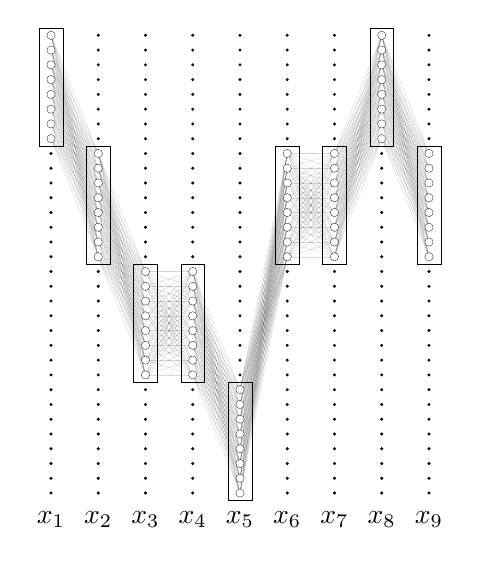
\begin{tikzpicture}%
\path[draw,line width=0.1pt,opacity=0.15,fill=black] (0.6,4.5) -- (1.2,3.0);%
\path[draw,line width=0.1pt,opacity=0.15,fill=black] (0.6,4.5) -- (1.2,3.1875);%
\path[draw,line width=0.1pt,opacity=0.15,fill=black] (0.6,4.5) -- (1.2,3.375);%
\path[draw,line width=0.1pt,opacity=0.15,fill=black] (0.6,4.5) -- (1.2,3.5625);%
\path[draw,line width=0.1pt,opacity=0.15,fill=black] (0.6,4.5) -- (1.2,3.75);%
\path[draw,line width=0.1pt,opacity=0.15,fill=black] (0.6,4.5) -- (1.2,3.9375);%
\path[draw,line width=0.1pt,opacity=0.15,fill=black] (0.6,4.5) -- (1.2,4.125);%
\path[draw,line width=0.1pt,opacity=0.15,fill=black] (0.6,4.5) -- (1.2,4.3125);%
\path[draw,line width=0.1pt,opacity=0.15,fill=black] (0.6,4.6875) -- (1.2,3.0);%
\path[draw,line width=0.1pt,opacity=0.15,fill=black] (0.6,4.6875) -- (1.2,3.1875);%
\path[draw,line width=0.1pt,opacity=0.15,fill=black] (0.6,4.6875) -- (1.2,3.375);%
\path[draw,line width=0.1pt,opacity=0.15,fill=black] (0.6,4.6875) -- (1.2,3.5625);%
\path[draw,line width=0.1pt,opacity=0.15,fill=black] (0.6,4.6875) -- (1.2,3.75);%
\path[draw,line width=0.1pt,opacity=0.15,fill=black] (0.6,4.6875) -- (1.2,3.9375);%
\path[draw,line width=0.1pt,opacity=0.15,fill=black] (0.6,4.6875) -- (1.2,4.125);%
\path[draw,line width=0.1pt,opacity=0.15,fill=black] (0.6,4.6875) -- (1.2,4.3125);%
\path[draw,line width=0.1pt,opacity=0.15,fill=black] (0.6,4.875) -- (1.2,3.0);%
\path[draw,line width=0.1pt,opacity=0.15,fill=black] (0.6,4.875) -- (1.2,3.1875);%
\path[draw,line width=0.1pt,opacity=0.15,fill=black] (0.6,4.875) -- (1.2,3.375);%
\path[draw,line width=0.1pt,opacity=0.15,fill=black] (0.6,4.875) -- (1.2,3.5625);%
\path[draw,line width=0.1pt,opacity=0.15,fill=black] (0.6,4.875) -- (1.2,3.75);%
\path[draw,line width=0.1pt,opacity=0.15,fill=black] (0.6,4.875) -- (1.2,3.9375);%
\path[draw,line width=0.1pt,opacity=0.15,fill=black] (0.6,4.875) -- (1.2,4.125);%
\path[draw,line width=0.1pt,opacity=0.15,fill=black] (0.6,4.875) -- (1.2,4.3125);%
\path[draw,line width=0.1pt,opacity=0.15,fill=black] (0.6,5.0625) -- (1.2,3.0);%
\path[draw,line width=0.1pt,opacity=0.15,fill=black] (0.6,5.0625) -- (1.2,3.1875);%
\path[draw,line width=0.1pt,opacity=0.15,fill=black] (0.6,5.0625) -- (1.2,3.375);%
\path[draw,line width=0.1pt,opacity=0.15,fill=black] (0.6,5.0625) -- (1.2,3.5625);%
\path[draw,line width=0.1pt,opacity=0.15,fill=black] (0.6,5.0625) -- (1.2,3.75);%
\path[draw,line width=0.1pt,opacity=0.15,fill=black] (0.6,5.0625) -- (1.2,3.9375);%
\path[draw,line width=0.1pt,opacity=0.15,fill=black] (0.6,5.0625) -- (1.2,4.125);%
\path[draw,line width=0.1pt,opacity=0.15,fill=black] (0.6,5.0625) -- (1.2,4.3125);%
\path[draw,line width=0.1pt,opacity=0.15,fill=black] (0.6,5.25) -- (1.2,3.0);%
\path[draw,line width=0.1pt,opacity=0.15,fill=black] (0.6,5.25) -- (1.2,3.1875);%
\path[draw,line width=0.1pt,opacity=0.15,fill=black] (0.6,5.25) -- (1.2,3.375);%
\path[draw,line width=0.1pt,opacity=0.15,fill=black] (0.6,5.25) -- (1.2,3.5625);%
\path[draw,line width=0.1pt,opacity=0.15,fill=black] (0.6,5.25) -- (1.2,3.75);%
\path[draw,line width=0.1pt,opacity=0.15,fill=black] (0.6,5.25) -- (1.2,3.9375);%
\path[draw,line width=0.1pt,opacity=0.15,fill=black] (0.6,5.25) -- (1.2,4.125);%
\path[draw,line width=0.1pt,opacity=0.15,fill=black] (0.6,5.25) -- (1.2,4.3125);%
\path[draw,line width=0.1pt,opacity=0.15,fill=black] (0.6,5.4375) -- (1.2,3.0);%
\path[draw,line width=0.1pt,opacity=0.15,fill=black] (0.6,5.4375) -- (1.2,3.1875);%
\path[draw,line width=0.1pt,opacity=0.15,fill=black] (0.6,5.4375) -- (1.2,3.375);%
\path[draw,line width=0.1pt,opacity=0.15,fill=black] (0.6,5.4375) -- (1.2,3.5625);%
\path[draw,line width=0.1pt,opacity=0.15,fill=black] (0.6,5.4375) -- (1.2,3.75);%
\path[draw,line width=0.1pt,opacity=0.15,fill=black] (0.6,5.4375) -- (1.2,3.9375);%
\path[draw,line width=0.1pt,opacity=0.15,fill=black] (0.6,5.4375) -- (1.2,4.125);%
\path[draw,line width=0.1pt,opacity=0.15,fill=black] (0.6,5.4375) -- (1.2,4.3125);%
\path[draw,line width=0.1pt,opacity=0.15,fill=black] (0.6,5.625) -- (1.2,3.0);%
\path[draw,line width=0.1pt,opacity=0.15,fill=black] (0.6,5.625) -- (1.2,3.1875);%
\path[draw,line width=0.1pt,opacity=0.15,fill=black] (0.6,5.625) -- (1.2,3.375);%
\path[draw,line width=0.1pt,opacity=0.15,fill=black] (0.6,5.625) -- (1.2,3.5625);%
\path[draw,line width=0.1pt,opacity=0.15,fill=black] (0.6,5.625) -- (1.2,3.75);%
\path[draw,line width=0.1pt,opacity=0.15,fill=black] (0.6,5.625) -- (1.2,3.9375);%
\path[draw,line width=0.1pt,opacity=0.15,fill=black] (0.6,5.625) -- (1.2,4.125);%
\path[draw,line width=0.1pt,opacity=0.15,fill=black] (0.6,5.625) -- (1.2,4.3125);%
\path[draw,line width=0.1pt,opacity=0.15,fill=black] (0.6,5.8125) -- (1.2,3.0);%
\path[draw,line width=0.1pt,opacity=0.15,fill=black] (0.6,5.8125) -- (1.2,3.1875);%
\path[draw,line width=0.1pt,opacity=0.15,fill=black] (0.6,5.8125) -- (1.2,3.375);%
\path[draw,line width=0.1pt,opacity=0.15,fill=black] (0.6,5.8125) -- (1.2,3.5625);%
\path[draw,line width=0.1pt,opacity=0.15,fill=black] (0.6,5.8125) -- (1.2,3.75);%
\path[draw,line width=0.1pt,opacity=0.15,fill=black] (0.6,5.8125) -- (1.2,3.9375);%
\path[draw,line width=0.1pt,opacity=0.15,fill=black] (0.6,5.8125) -- (1.2,4.125);%
\path[draw,line width=0.1pt,opacity=0.15,fill=black] (0.6,5.8125) -- (1.2,4.3125);%
\path[draw,line width=0.1pt,opacity=0.15,fill=black] (1.2,3.0) -- (1.8,1.5);%
\path[draw,line width=0.1pt,opacity=0.15,fill=black] (1.2,3.0) -- (1.8,1.6875);%
\path[draw,line width=0.1pt,opacity=0.15,fill=black] (1.2,3.0) -- (1.8,1.875);%
\path[draw,line width=0.1pt,opacity=0.15,fill=black] (1.2,3.0) -- (1.8,2.0625);%
\path[draw,line width=0.1pt,opacity=0.15,fill=black] (1.2,3.0) -- (1.8,2.25);%
\path[draw,line width=0.1pt,opacity=0.15,fill=black] (1.2,3.0) -- (1.8,2.4375);%
\path[draw,line width=0.1pt,opacity=0.15,fill=black] (1.2,3.0) -- (1.8,2.625);%
\path[draw,line width=0.1pt,opacity=0.15,fill=black] (1.2,3.0) -- (1.8,2.8125);%
\path[draw,line width=0.1pt,opacity=0.15,fill=black] (1.2,3.1875) -- (1.8,1.5);%
\path[draw,line width=0.1pt,opacity=0.15,fill=black] (1.2,3.1875) -- (1.8,1.6875);%
\path[draw,line width=0.1pt,opacity=0.15,fill=black] (1.2,3.1875) -- (1.8,1.875);%
\path[draw,line width=0.1pt,opacity=0.15,fill=black] (1.2,3.1875) -- (1.8,2.0625);%
\path[draw,line width=0.1pt,opacity=0.15,fill=black] (1.2,3.1875) -- (1.8,2.25);%
\path[draw,line width=0.1pt,opacity=0.15,fill=black] (1.2,3.1875) -- (1.8,2.4375);%
\path[draw,line width=0.1pt,opacity=0.15,fill=black] (1.2,3.1875) -- (1.8,2.625);%
\path[draw,line width=0.1pt,opacity=0.15,fill=black] (1.2,3.1875) -- (1.8,2.8125);%
\path[draw,line width=0.1pt,opacity=0.15,fill=black] (1.2,3.375) -- (1.8,1.5);%
\path[draw,line width=0.1pt,opacity=0.15,fill=black] (1.2,3.375) -- (1.8,1.6875);%
\path[draw,line width=0.1pt,opacity=0.15,fill=black] (1.2,3.375) -- (1.8,1.875);%
\path[draw,line width=0.1pt,opacity=0.15,fill=black] (1.2,3.375) -- (1.8,2.0625);%
\path[draw,line width=0.1pt,opacity=0.15,fill=black] (1.2,3.375) -- (1.8,2.25);%
\path[draw,line width=0.1pt,opacity=0.15,fill=black] (1.2,3.375) -- (1.8,2.4375);%
\path[draw,line width=0.1pt,opacity=0.15,fill=black] (1.2,3.375) -- (1.8,2.625);%
\path[draw,line width=0.1pt,opacity=0.15,fill=black] (1.2,3.375) -- (1.8,2.8125);%
\path[draw,line width=0.1pt,opacity=0.15,fill=black] (1.2,3.5625) -- (1.8,1.5);%
\path[draw,line width=0.1pt,opacity=0.15,fill=black] (1.2,3.5625) -- (1.8,1.6875);%
\path[draw,line width=0.1pt,opacity=0.15,fill=black] (1.2,3.5625) -- (1.8,1.875);%
\path[draw,line width=0.1pt,opacity=0.15,fill=black] (1.2,3.5625) -- (1.8,2.0625);%
\path[draw,line width=0.1pt,opacity=0.15,fill=black] (1.2,3.5625) -- (1.8,2.25);%
\path[draw,line width=0.1pt,opacity=0.15,fill=black] (1.2,3.5625) -- (1.8,2.4375);%
\path[draw,line width=0.1pt,opacity=0.15,fill=black] (1.2,3.5625) -- (1.8,2.625);%
\path[draw,line width=0.1pt,opacity=0.15,fill=black] (1.2,3.5625) -- (1.8,2.8125);%
\path[draw,line width=0.1pt,opacity=0.15,fill=black] (1.2,3.75) -- (1.8,1.5);%
\path[draw,line width=0.1pt,opacity=0.15,fill=black] (1.2,3.75) -- (1.8,1.6875);%
\path[draw,line width=0.1pt,opacity=0.15,fill=black] (1.2,3.75) -- (1.8,1.875);%
\path[draw,line width=0.1pt,opacity=0.15,fill=black] (1.2,3.75) -- (1.8,2.0625);%
\path[draw,line width=0.1pt,opacity=0.15,fill=black] (1.2,3.75) -- (1.8,2.25);%
\path[draw,line width=0.1pt,opacity=0.15,fill=black] (1.2,3.75) -- (1.8,2.4375);%
\path[draw,line width=0.1pt,opacity=0.15,fill=black] (1.2,3.75) -- (1.8,2.625);%
\path[draw,line width=0.1pt,opacity=0.15,fill=black] (1.2,3.75) -- (1.8,2.8125);%
\path[draw,line width=0.1pt,opacity=0.15,fill=black] (1.2,3.9375) -- (1.8,1.5);%
\path[draw,line width=0.1pt,opacity=0.15,fill=black] (1.2,3.9375) -- (1.8,1.6875);%
\path[draw,line width=0.1pt,opacity=0.15,fill=black] (1.2,3.9375) -- (1.8,1.875);%
\path[draw,line width=0.1pt,opacity=0.15,fill=black] (1.2,3.9375) -- (1.8,2.0625);%
\path[draw,line width=0.1pt,opacity=0.15,fill=black] (1.2,3.9375) -- (1.8,2.25);%
\path[draw,line width=0.1pt,opacity=0.15,fill=black] (1.2,3.9375) -- (1.8,2.4375);%
\path[draw,line width=0.1pt,opacity=0.15,fill=black] (1.2,3.9375) -- (1.8,2.625);%
\path[draw,line width=0.1pt,opacity=0.15,fill=black] (1.2,3.9375) -- (1.8,2.8125);%
\path[draw,line width=0.1pt,opacity=0.15,fill=black] (1.2,4.125) -- (1.8,1.5);%
\path[draw,line width=0.1pt,opacity=0.15,fill=black] (1.2,4.125) -- (1.8,1.6875);%
\path[draw,line width=0.1pt,opacity=0.15,fill=black] (1.2,4.125) -- (1.8,1.875);%
\path[draw,line width=0.1pt,opacity=0.15,fill=black] (1.2,4.125) -- (1.8,2.0625);%
\path[draw,line width=0.1pt,opacity=0.15,fill=black] (1.2,4.125) -- (1.8,2.25);%
\path[draw,line width=0.1pt,opacity=0.15,fill=black] (1.2,4.125) -- (1.8,2.4375);%
\path[draw,line width=0.1pt,opacity=0.15,fill=black] (1.2,4.125) -- (1.8,2.625);%
\path[draw,line width=0.1pt,opacity=0.15,fill=black] (1.2,4.125) -- (1.8,2.8125);%
\path[draw,line width=0.1pt,opacity=0.15,fill=black] (1.2,4.3125) -- (1.8,1.5);%
\path[draw,line width=0.1pt,opacity=0.15,fill=black] (1.2,4.3125) -- (1.8,1.6875);%
\path[draw,line width=0.1pt,opacity=0.15,fill=black] (1.2,4.3125) -- (1.8,1.875);%
\path[draw,line width=0.1pt,opacity=0.15,fill=black] (1.2,4.3125) -- (1.8,2.0625);%
\path[draw,line width=0.1pt,opacity=0.15,fill=black] (1.2,4.3125) -- (1.8,2.25);%
\path[draw,line width=0.1pt,opacity=0.15,fill=black] (1.2,4.3125) -- (1.8,2.4375);%
\path[draw,line width=0.1pt,opacity=0.15,fill=black] (1.2,4.3125) -- (1.8,2.625);%
\path[draw,line width=0.1pt,opacity=0.15,fill=black] (1.2,4.3125) -- (1.8,2.8125);%
\path[draw,line width=0.1pt,opacity=0.15,fill=black] (1.8,1.5) -- (2.4,1.5);%
\path[draw,line width=0.1pt,opacity=0.15,fill=black] (1.8,1.5) -- (2.4,1.6875);%
\path[draw,line width=0.1pt,opacity=0.15,fill=black] (1.8,1.5) -- (2.4,1.875);%
\path[draw,line width=0.1pt,opacity=0.15,fill=black] (1.8,1.5) -- (2.4,2.0625);%
\path[draw,line width=0.1pt,opacity=0.15,fill=black] (1.8,1.5) -- (2.4,2.25);%
\path[draw,line width=0.1pt,opacity=0.15,fill=black] (1.8,1.5) -- (2.4,2.4375);%
\path[draw,line width=0.1pt,opacity=0.15,fill=black] (1.8,1.5) -- (2.4,2.625);%
\path[draw,line width=0.1pt,opacity=0.15,fill=black] (1.8,1.5) -- (2.4,2.8125);%
\path[draw,line width=0.1pt,opacity=0.15,fill=black] (1.8,1.6875) -- (2.4,1.5);%
\path[draw,line width=0.1pt,opacity=0.15,fill=black] (1.8,1.6875) -- (2.4,1.6875);%
\path[draw,line width=0.1pt,opacity=0.15,fill=black] (1.8,1.6875) -- (2.4,1.875);%
\path[draw,line width=0.1pt,opacity=0.15,fill=black] (1.8,1.6875) -- (2.4,2.0625);%
\path[draw,line width=0.1pt,opacity=0.15,fill=black] (1.8,1.6875) -- (2.4,2.25);%
\path[draw,line width=0.1pt,opacity=0.15,fill=black] (1.8,1.6875) -- (2.4,2.4375);%
\path[draw,line width=0.1pt,opacity=0.15,fill=black] (1.8,1.6875) -- (2.4,2.625);%
\path[draw,line width=0.1pt,opacity=0.15,fill=black] (1.8,1.6875) -- (2.4,2.8125);%
\path[draw,line width=0.1pt,opacity=0.15,fill=black] (1.8,1.875) -- (2.4,1.5);%
\path[draw,line width=0.1pt,opacity=0.15,fill=black] (1.8,1.875) -- (2.4,1.6875);%
\path[draw,line width=0.1pt,opacity=0.15,fill=black] (1.8,1.875) -- (2.4,1.875);%
\path[draw,line width=0.1pt,opacity=0.15,fill=black] (1.8,1.875) -- (2.4,2.0625);%
\path[draw,line width=0.1pt,opacity=0.15,fill=black] (1.8,1.875) -- (2.4,2.25);%
\path[draw,line width=0.1pt,opacity=0.15,fill=black] (1.8,1.875) -- (2.4,2.4375);%
\path[draw,line width=0.1pt,opacity=0.15,fill=black] (1.8,1.875) -- (2.4,2.625);%
\path[draw,line width=0.1pt,opacity=0.15,fill=black] (1.8,1.875) -- (2.4,2.8125);%
\path[draw,line width=0.1pt,opacity=0.15,fill=black] (1.8,2.0625) -- (2.4,1.5);%
\path[draw,line width=0.1pt,opacity=0.15,fill=black] (1.8,2.0625) -- (2.4,1.6875);%
\path[draw,line width=0.1pt,opacity=0.15,fill=black] (1.8,2.0625) -- (2.4,1.875);%
\path[draw,line width=0.1pt,opacity=0.15,fill=black] (1.8,2.0625) -- (2.4,2.0625);%
\path[draw,line width=0.1pt,opacity=0.15,fill=black] (1.8,2.0625) -- (2.4,2.25);%
\path[draw,line width=0.1pt,opacity=0.15,fill=black] (1.8,2.0625) -- (2.4,2.4375);%
\path[draw,line width=0.1pt,opacity=0.15,fill=black] (1.8,2.0625) -- (2.4,2.625);%
\path[draw,line width=0.1pt,opacity=0.15,fill=black] (1.8,2.0625) -- (2.4,2.8125);%
\path[draw,line width=0.1pt,opacity=0.15,fill=black] (1.8,2.25) -- (2.4,1.5);%
\path[draw,line width=0.1pt,opacity=0.15,fill=black] (1.8,2.25) -- (2.4,1.6875);%
\path[draw,line width=0.1pt,opacity=0.15,fill=black] (1.8,2.25) -- (2.4,1.875);%
\path[draw,line width=0.1pt,opacity=0.15,fill=black] (1.8,2.25) -- (2.4,2.0625);%
\path[draw,line width=0.1pt,opacity=0.15,fill=black] (1.8,2.25) -- (2.4,2.25);%
\path[draw,line width=0.1pt,opacity=0.15,fill=black] (1.8,2.25) -- (2.4,2.4375);%
\path[draw,line width=0.1pt,opacity=0.15,fill=black] (1.8,2.25) -- (2.4,2.625);%
\path[draw,line width=0.1pt,opacity=0.15,fill=black] (1.8,2.25) -- (2.4,2.8125);%
\path[draw,line width=0.1pt,opacity=0.15,fill=black] (1.8,2.4375) -- (2.4,1.5);%
\path[draw,line width=0.1pt,opacity=0.15,fill=black] (1.8,2.4375) -- (2.4,1.6875);%
\path[draw,line width=0.1pt,opacity=0.15,fill=black] (1.8,2.4375) -- (2.4,1.875);%
\path[draw,line width=0.1pt,opacity=0.15,fill=black] (1.8,2.4375) -- (2.4,2.0625);%
\path[draw,line width=0.1pt,opacity=0.15,fill=black] (1.8,2.4375) -- (2.4,2.25);%
\path[draw,line width=0.1pt,opacity=0.15,fill=black] (1.8,2.4375) -- (2.4,2.4375);%
\path[draw,line width=0.1pt,opacity=0.15,fill=black] (1.8,2.4375) -- (2.4,2.625);%
\path[draw,line width=0.1pt,opacity=0.15,fill=black] (1.8,2.4375) -- (2.4,2.8125);%
\path[draw,line width=0.1pt,opacity=0.15,fill=black] (1.8,2.625) -- (2.4,1.5);%
\path[draw,line width=0.1pt,opacity=0.15,fill=black] (1.8,2.625) -- (2.4,1.6875);%
\path[draw,line width=0.1pt,opacity=0.15,fill=black] (1.8,2.625) -- (2.4,1.875);%
\path[draw,line width=0.1pt,opacity=0.15,fill=black] (1.8,2.625) -- (2.4,2.0625);%
\path[draw,line width=0.1pt,opacity=0.15,fill=black] (1.8,2.625) -- (2.4,2.25);%
\path[draw,line width=0.1pt,opacity=0.15,fill=black] (1.8,2.625) -- (2.4,2.4375);%
\path[draw,line width=0.1pt,opacity=0.15,fill=black] (1.8,2.625) -- (2.4,2.625);%
\path[draw,line width=0.1pt,opacity=0.15,fill=black] (1.8,2.625) -- (2.4,2.8125);%
\path[draw,line width=0.1pt,opacity=0.15,fill=black] (1.8,2.8125) -- (2.4,1.5);%
\path[draw,line width=0.1pt,opacity=0.15,fill=black] (1.8,2.8125) -- (2.4,1.6875);%
\path[draw,line width=0.1pt,opacity=0.15,fill=black] (1.8,2.8125) -- (2.4,1.875);%
\path[draw,line width=0.1pt,opacity=0.15,fill=black] (1.8,2.8125) -- (2.4,2.0625);%
\path[draw,line width=0.1pt,opacity=0.15,fill=black] (1.8,2.8125) -- (2.4,2.25);%
\path[draw,line width=0.1pt,opacity=0.15,fill=black] (1.8,2.8125) -- (2.4,2.4375);%
\path[draw,line width=0.1pt,opacity=0.15,fill=black] (1.8,2.8125) -- (2.4,2.625);%
\path[draw,line width=0.1pt,opacity=0.15,fill=black] (1.8,2.8125) -- (2.4,2.8125);%
\path[draw,line width=0.1pt,opacity=0.15,fill=black] (2.4,1.5) -- (3.0,0.0);%
\path[draw,line width=0.1pt,opacity=0.15,fill=black] (2.4,1.5) -- (3.0,0.1875);%
\path[draw,line width=0.1pt,opacity=0.15,fill=black] (2.4,1.5) -- (3.0,0.375);%
\path[draw,line width=0.1pt,opacity=0.15,fill=black] (2.4,1.5) -- (3.0,0.5625);%
\path[draw,line width=0.1pt,opacity=0.15,fill=black] (2.4,1.5) -- (3.0,0.75);%
\path[draw,line width=0.1pt,opacity=0.15,fill=black] (2.4,1.5) -- (3.0,0.9375);%
\path[draw,line width=0.1pt,opacity=0.15,fill=black] (2.4,1.5) -- (3.0,1.125);%
\path[draw,line width=0.1pt,opacity=0.15,fill=black] (2.4,1.5) -- (3.0,1.3125);%
\path[draw,line width=0.1pt,opacity=0.15,fill=black] (2.4,1.6875) -- (3.0,0.0);%
\path[draw,line width=0.1pt,opacity=0.15,fill=black] (2.4,1.6875) -- (3.0,0.1875);%
\path[draw,line width=0.1pt,opacity=0.15,fill=black] (2.4,1.6875) -- (3.0,0.375);%
\path[draw,line width=0.1pt,opacity=0.15,fill=black] (2.4,1.6875) -- (3.0,0.5625);%
\path[draw,line width=0.1pt,opacity=0.15,fill=black] (2.4,1.6875) -- (3.0,0.75);%
\path[draw,line width=0.1pt,opacity=0.15,fill=black] (2.4,1.6875) -- (3.0,0.9375);%
\path[draw,line width=0.1pt,opacity=0.15,fill=black] (2.4,1.6875) -- (3.0,1.125);%
\path[draw,line width=0.1pt,opacity=0.15,fill=black] (2.4,1.6875) -- (3.0,1.3125);%
\path[draw,line width=0.1pt,opacity=0.15,fill=black] (2.4,1.875) -- (3.0,0.0);%
\path[draw,line width=0.1pt,opacity=0.15,fill=black] (2.4,1.875) -- (3.0,0.1875);%
\path[draw,line width=0.1pt,opacity=0.15,fill=black] (2.4,1.875) -- (3.0,0.375);%
\path[draw,line width=0.1pt,opacity=0.15,fill=black] (2.4,1.875) -- (3.0,0.5625);%
\path[draw,line width=0.1pt,opacity=0.15,fill=black] (2.4,1.875) -- (3.0,0.75);%
\path[draw,line width=0.1pt,opacity=0.15,fill=black] (2.4,1.875) -- (3.0,0.9375);%
\path[draw,line width=0.1pt,opacity=0.15,fill=black] (2.4,1.875) -- (3.0,1.125);%
\path[draw,line width=0.1pt,opacity=0.15,fill=black] (2.4,1.875) -- (3.0,1.3125);%
\path[draw,line width=0.1pt,opacity=0.15,fill=black] (2.4,2.0625) -- (3.0,0.0);%
\path[draw,line width=0.1pt,opacity=0.15,fill=black] (2.4,2.0625) -- (3.0,0.1875);%
\path[draw,line width=0.1pt,opacity=0.15,fill=black] (2.4,2.0625) -- (3.0,0.375);%
\path[draw,line width=0.1pt,opacity=0.15,fill=black] (2.4,2.0625) -- (3.0,0.5625);%
\path[draw,line width=0.1pt,opacity=0.15,fill=black] (2.4,2.0625) -- (3.0,0.75);%
\path[draw,line width=0.1pt,opacity=0.15,fill=black] (2.4,2.0625) -- (3.0,0.9375);%
\path[draw,line width=0.1pt,opacity=0.15,fill=black] (2.4,2.0625) -- (3.0,1.125);%
\path[draw,line width=0.1pt,opacity=0.15,fill=black] (2.4,2.0625) -- (3.0,1.3125);%
\path[draw,line width=0.1pt,opacity=0.15,fill=black] (2.4,2.25) -- (3.0,0.0);%
\path[draw,line width=0.1pt,opacity=0.15,fill=black] (2.4,2.25) -- (3.0,0.1875);%
\path[draw,line width=0.1pt,opacity=0.15,fill=black] (2.4,2.25) -- (3.0,0.375);%
\path[draw,line width=0.1pt,opacity=0.15,fill=black] (2.4,2.25) -- (3.0,0.5625);%
\path[draw,line width=0.1pt,opacity=0.15,fill=black] (2.4,2.25) -- (3.0,0.75);%
\path[draw,line width=0.1pt,opacity=0.15,fill=black] (2.4,2.25) -- (3.0,0.9375);%
\path[draw,line width=0.1pt,opacity=0.15,fill=black] (2.4,2.25) -- (3.0,1.125);%
\path[draw,line width=0.1pt,opacity=0.15,fill=black] (2.4,2.25) -- (3.0,1.3125);%
\path[draw,line width=0.1pt,opacity=0.15,fill=black] (2.4,2.4375) -- (3.0,0.0);%
\path[draw,line width=0.1pt,opacity=0.15,fill=black] (2.4,2.4375) -- (3.0,0.1875);%
\path[draw,line width=0.1pt,opacity=0.15,fill=black] (2.4,2.4375) -- (3.0,0.375);%
\path[draw,line width=0.1pt,opacity=0.15,fill=black] (2.4,2.4375) -- (3.0,0.5625);%
\path[draw,line width=0.1pt,opacity=0.15,fill=black] (2.4,2.4375) -- (3.0,0.75);%
\path[draw,line width=0.1pt,opacity=0.15,fill=black] (2.4,2.4375) -- (3.0,0.9375);%
\path[draw,line width=0.1pt,opacity=0.15,fill=black] (2.4,2.4375) -- (3.0,1.125);%
\path[draw,line width=0.1pt,opacity=0.15,fill=black] (2.4,2.4375) -- (3.0,1.3125);%
\path[draw,line width=0.1pt,opacity=0.15,fill=black] (2.4,2.625) -- (3.0,0.0);%
\path[draw,line width=0.1pt,opacity=0.15,fill=black] (2.4,2.625) -- (3.0,0.1875);%
\path[draw,line width=0.1pt,opacity=0.15,fill=black] (2.4,2.625) -- (3.0,0.375);%
\path[draw,line width=0.1pt,opacity=0.15,fill=black] (2.4,2.625) -- (3.0,0.5625);%
\path[draw,line width=0.1pt,opacity=0.15,fill=black] (2.4,2.625) -- (3.0,0.75);%
\path[draw,line width=0.1pt,opacity=0.15,fill=black] (2.4,2.625) -- (3.0,0.9375);%
\path[draw,line width=0.1pt,opacity=0.15,fill=black] (2.4,2.625) -- (3.0,1.125);%
\path[draw,line width=0.1pt,opacity=0.15,fill=black] (2.4,2.625) -- (3.0,1.3125);%
\path[draw,line width=0.1pt,opacity=0.15,fill=black] (2.4,2.8125) -- (3.0,0.0);%
\path[draw,line width=0.1pt,opacity=0.15,fill=black] (2.4,2.8125) -- (3.0,0.1875);%
\path[draw,line width=0.1pt,opacity=0.15,fill=black] (2.4,2.8125) -- (3.0,0.375);%
\path[draw,line width=0.1pt,opacity=0.15,fill=black] (2.4,2.8125) -- (3.0,0.5625);%
\path[draw,line width=0.1pt,opacity=0.15,fill=black] (2.4,2.8125) -- (3.0,0.75);%
\path[draw,line width=0.1pt,opacity=0.15,fill=black] (2.4,2.8125) -- (3.0,0.9375);%
\path[draw,line width=0.1pt,opacity=0.15,fill=black] (2.4,2.8125) -- (3.0,1.125);%
\path[draw,line width=0.1pt,opacity=0.15,fill=black] (2.4,2.8125) -- (3.0,1.3125);%
\path[draw,line width=0.1pt,opacity=0.15,fill=black] (3.0,0.0) -- (3.6,3.0);%
\path[draw,line width=0.1pt,opacity=0.15,fill=black] (3.0,0.0) -- (3.6,3.1875);%
\path[draw,line width=0.1pt,opacity=0.15,fill=black] (3.0,0.0) -- (3.6,3.375);%
\path[draw,line width=0.1pt,opacity=0.15,fill=black] (3.0,0.0) -- (3.6,3.5625);%
\path[draw,line width=0.1pt,opacity=0.15,fill=black] (3.0,0.0) -- (3.6,3.75);%
\path[draw,line width=0.1pt,opacity=0.15,fill=black] (3.0,0.0) -- (3.6,3.9375);%
\path[draw,line width=0.1pt,opacity=0.15,fill=black] (3.0,0.0) -- (3.6,4.125);%
\path[draw,line width=0.1pt,opacity=0.15,fill=black] (3.0,0.0) -- (3.6,4.3125);%
\path[draw,line width=0.1pt,opacity=0.15,fill=black] (3.0,0.1875) -- (3.6,3.0);%
\path[draw,line width=0.1pt,opacity=0.15,fill=black] (3.0,0.1875) -- (3.6,3.1875);%
\path[draw,line width=0.1pt,opacity=0.15,fill=black] (3.0,0.1875) -- (3.6,3.375);%
\path[draw,line width=0.1pt,opacity=0.15,fill=black] (3.0,0.1875) -- (3.6,3.5625);%
\path[draw,line width=0.1pt,opacity=0.15,fill=black] (3.0,0.1875) -- (3.6,3.75);%
\path[draw,line width=0.1pt,opacity=0.15,fill=black] (3.0,0.1875) -- (3.6,3.9375);%
\path[draw,line width=0.1pt,opacity=0.15,fill=black] (3.0,0.1875) -- (3.6,4.125);%
\path[draw,line width=0.1pt,opacity=0.15,fill=black] (3.0,0.1875) -- (3.6,4.3125);%
\path[draw,line width=0.1pt,opacity=0.15,fill=black] (3.0,0.375) -- (3.6,3.0);%
\path[draw,line width=0.1pt,opacity=0.15,fill=black] (3.0,0.375) -- (3.6,3.1875);%
\path[draw,line width=0.1pt,opacity=0.15,fill=black] (3.0,0.375) -- (3.6,3.375);%
\path[draw,line width=0.1pt,opacity=0.15,fill=black] (3.0,0.375) -- (3.6,3.5625);%
\path[draw,line width=0.1pt,opacity=0.15,fill=black] (3.0,0.375) -- (3.6,3.75);%
\path[draw,line width=0.1pt,opacity=0.15,fill=black] (3.0,0.375) -- (3.6,3.9375);%
\path[draw,line width=0.1pt,opacity=0.15,fill=black] (3.0,0.375) -- (3.6,4.125);%
\path[draw,line width=0.1pt,opacity=0.15,fill=black] (3.0,0.375) -- (3.6,4.3125);%
\path[draw,line width=0.1pt,opacity=0.15,fill=black] (3.0,0.5625) -- (3.6,3.0);%
\path[draw,line width=0.1pt,opacity=0.15,fill=black] (3.0,0.5625) -- (3.6,3.1875);%
\path[draw,line width=0.1pt,opacity=0.15,fill=black] (3.0,0.5625) -- (3.6,3.375);%
\path[draw,line width=0.1pt,opacity=0.15,fill=black] (3.0,0.5625) -- (3.6,3.5625);%
\path[draw,line width=0.1pt,opacity=0.15,fill=black] (3.0,0.5625) -- (3.6,3.75);%
\path[draw,line width=0.1pt,opacity=0.15,fill=black] (3.0,0.5625) -- (3.6,3.9375);%
\path[draw,line width=0.1pt,opacity=0.15,fill=black] (3.0,0.5625) -- (3.6,4.125);%
\path[draw,line width=0.1pt,opacity=0.15,fill=black] (3.0,0.5625) -- (3.6,4.3125);%
\path[draw,line width=0.1pt,opacity=0.15,fill=black] (3.0,0.75) -- (3.6,3.0);%
\path[draw,line width=0.1pt,opacity=0.15,fill=black] (3.0,0.75) -- (3.6,3.1875);%
\path[draw,line width=0.1pt,opacity=0.15,fill=black] (3.0,0.75) -- (3.6,3.375);%
\path[draw,line width=0.1pt,opacity=0.15,fill=black] (3.0,0.75) -- (3.6,3.5625);%
\path[draw,line width=0.1pt,opacity=0.15,fill=black] (3.0,0.75) -- (3.6,3.75);%
\path[draw,line width=0.1pt,opacity=0.15,fill=black] (3.0,0.75) -- (3.6,3.9375);%
\path[draw,line width=0.1pt,opacity=0.15,fill=black] (3.0,0.75) -- (3.6,4.125);%
\path[draw,line width=0.1pt,opacity=0.15,fill=black] (3.0,0.75) -- (3.6,4.3125);%
\path[draw,line width=0.1pt,opacity=0.15,fill=black] (3.0,0.9375) -- (3.6,3.0);%
\path[draw,line width=0.1pt,opacity=0.15,fill=black] (3.0,0.9375) -- (3.6,3.1875);%
\path[draw,line width=0.1pt,opacity=0.15,fill=black] (3.0,0.9375) -- (3.6,3.375);%
\path[draw,line width=0.1pt,opacity=0.15,fill=black] (3.0,0.9375) -- (3.6,3.5625);%
\path[draw,line width=0.1pt,opacity=0.15,fill=black] (3.0,0.9375) -- (3.6,3.75);%
\path[draw,line width=0.1pt,opacity=0.15,fill=black] (3.0,0.9375) -- (3.6,3.9375);%
\path[draw,line width=0.1pt,opacity=0.15,fill=black] (3.0,0.9375) -- (3.6,4.125);%
\path[draw,line width=0.1pt,opacity=0.15,fill=black] (3.0,0.9375) -- (3.6,4.3125);%
\path[draw,line width=0.1pt,opacity=0.15,fill=black] (3.0,1.125) -- (3.6,3.0);%
\path[draw,line width=0.1pt,opacity=0.15,fill=black] (3.0,1.125) -- (3.6,3.1875);%
\path[draw,line width=0.1pt,opacity=0.15,fill=black] (3.0,1.125) -- (3.6,3.375);%
\path[draw,line width=0.1pt,opacity=0.15,fill=black] (3.0,1.125) -- (3.6,3.5625);%
\path[draw,line width=0.1pt,opacity=0.15,fill=black] (3.0,1.125) -- (3.6,3.75);%
\path[draw,line width=0.1pt,opacity=0.15,fill=black] (3.0,1.125) -- (3.6,3.9375);%
\path[draw,line width=0.1pt,opacity=0.15,fill=black] (3.0,1.125) -- (3.6,4.125);%
\path[draw,line width=0.1pt,opacity=0.15,fill=black] (3.0,1.125) -- (3.6,4.3125);%
\path[draw,line width=0.1pt,opacity=0.15,fill=black] (3.0,1.3125) -- (3.6,3.0);%
\path[draw,line width=0.1pt,opacity=0.15,fill=black] (3.0,1.3125) -- (3.6,3.1875);%
\path[draw,line width=0.1pt,opacity=0.15,fill=black] (3.0,1.3125) -- (3.6,3.375);%
\path[draw,line width=0.1pt,opacity=0.15,fill=black] (3.0,1.3125) -- (3.6,3.5625);%
\path[draw,line width=0.1pt,opacity=0.15,fill=black] (3.0,1.3125) -- (3.6,3.75);%
\path[draw,line width=0.1pt,opacity=0.15,fill=black] (3.0,1.3125) -- (3.6,3.9375);%
\path[draw,line width=0.1pt,opacity=0.15,fill=black] (3.0,1.3125) -- (3.6,4.125);%
\path[draw,line width=0.1pt,opacity=0.15,fill=black] (3.0,1.3125) -- (3.6,4.3125);%
\path[draw,line width=0.1pt,opacity=0.15,fill=black] (3.6,3.0) -- (4.2,3.0);%
\path[draw,line width=0.1pt,opacity=0.15,fill=black] (3.6,3.0) -- (4.2,3.1875);%
\path[draw,line width=0.1pt,opacity=0.15,fill=black] (3.6,3.0) -- (4.2,3.375);%
\path[draw,line width=0.1pt,opacity=0.15,fill=black] (3.6,3.0) -- (4.2,3.5625);%
\path[draw,line width=0.1pt,opacity=0.15,fill=black] (3.6,3.0) -- (4.2,3.75);%
\path[draw,line width=0.1pt,opacity=0.15,fill=black] (3.6,3.0) -- (4.2,3.9375);%
\path[draw,line width=0.1pt,opacity=0.15,fill=black] (3.6,3.0) -- (4.2,4.125);%
\path[draw,line width=0.1pt,opacity=0.15,fill=black] (3.6,3.0) -- (4.2,4.3125);%
\path[draw,line width=0.1pt,opacity=0.15,fill=black] (3.6,3.1875) -- (4.2,3.0);%
\path[draw,line width=0.1pt,opacity=0.15,fill=black] (3.6,3.1875) -- (4.2,3.1875);%
\path[draw,line width=0.1pt,opacity=0.15,fill=black] (3.6,3.1875) -- (4.2,3.375);%
\path[draw,line width=0.1pt,opacity=0.15,fill=black] (3.6,3.1875) -- (4.2,3.5625);%
\path[draw,line width=0.1pt,opacity=0.15,fill=black] (3.6,3.1875) -- (4.2,3.75);%
\path[draw,line width=0.1pt,opacity=0.15,fill=black] (3.6,3.1875) -- (4.2,3.9375);%
\path[draw,line width=0.1pt,opacity=0.15,fill=black] (3.6,3.1875) -- (4.2,4.125);%
\path[draw,line width=0.1pt,opacity=0.15,fill=black] (3.6,3.1875) -- (4.2,4.3125);%
\path[draw,line width=0.1pt,opacity=0.15,fill=black] (3.6,3.375) -- (4.2,3.0);%
\path[draw,line width=0.1pt,opacity=0.15,fill=black] (3.6,3.375) -- (4.2,3.1875);%
\path[draw,line width=0.1pt,opacity=0.15,fill=black] (3.6,3.375) -- (4.2,3.375);%
\path[draw,line width=0.1pt,opacity=0.15,fill=black] (3.6,3.375) -- (4.2,3.5625);%
\path[draw,line width=0.1pt,opacity=0.15,fill=black] (3.6,3.375) -- (4.2,3.75);%
\path[draw,line width=0.1pt,opacity=0.15,fill=black] (3.6,3.375) -- (4.2,3.9375);%
\path[draw,line width=0.1pt,opacity=0.15,fill=black] (3.6,3.375) -- (4.2,4.125);%
\path[draw,line width=0.1pt,opacity=0.15,fill=black] (3.6,3.375) -- (4.2,4.3125);%
\path[draw,line width=0.1pt,opacity=0.15,fill=black] (3.6,3.5625) -- (4.2,3.0);%
\path[draw,line width=0.1pt,opacity=0.15,fill=black] (3.6,3.5625) -- (4.2,3.1875);%
\path[draw,line width=0.1pt,opacity=0.15,fill=black] (3.6,3.5625) -- (4.2,3.375);%
\path[draw,line width=0.1pt,opacity=0.15,fill=black] (3.6,3.5625) -- (4.2,3.5625);%
\path[draw,line width=0.1pt,opacity=0.15,fill=black] (3.6,3.5625) -- (4.2,3.75);%
\path[draw,line width=0.1pt,opacity=0.15,fill=black] (3.6,3.5625) -- (4.2,3.9375);%
\path[draw,line width=0.1pt,opacity=0.15,fill=black] (3.6,3.5625) -- (4.2,4.125);%
\path[draw,line width=0.1pt,opacity=0.15,fill=black] (3.6,3.5625) -- (4.2,4.3125);%
\path[draw,line width=0.1pt,opacity=0.15,fill=black] (3.6,3.75) -- (4.2,3.0);%
\path[draw,line width=0.1pt,opacity=0.15,fill=black] (3.6,3.75) -- (4.2,3.1875);%
\path[draw,line width=0.1pt,opacity=0.15,fill=black] (3.6,3.75) -- (4.2,3.375);%
\path[draw,line width=0.1pt,opacity=0.15,fill=black] (3.6,3.75) -- (4.2,3.5625);%
\path[draw,line width=0.1pt,opacity=0.15,fill=black] (3.6,3.75) -- (4.2,3.75);%
\path[draw,line width=0.1pt,opacity=0.15,fill=black] (3.6,3.75) -- (4.2,3.9375);%
\path[draw,line width=0.1pt,opacity=0.15,fill=black] (3.6,3.75) -- (4.2,4.125);%
\path[draw,line width=0.1pt,opacity=0.15,fill=black] (3.6,3.75) -- (4.2,4.3125);%
\path[draw,line width=0.1pt,opacity=0.15,fill=black] (3.6,3.9375) -- (4.2,3.0);%
\path[draw,line width=0.1pt,opacity=0.15,fill=black] (3.6,3.9375) -- (4.2,3.1875);%
\path[draw,line width=0.1pt,opacity=0.15,fill=black] (3.6,3.9375) -- (4.2,3.375);%
\path[draw,line width=0.1pt,opacity=0.15,fill=black] (3.6,3.9375) -- (4.2,3.5625);%
\path[draw,line width=0.1pt,opacity=0.15,fill=black] (3.6,3.9375) -- (4.2,3.75);%
\path[draw,line width=0.1pt,opacity=0.15,fill=black] (3.6,3.9375) -- (4.2,3.9375);%
\path[draw,line width=0.1pt,opacity=0.15,fill=black] (3.6,3.9375) -- (4.2,4.125);%
\path[draw,line width=0.1pt,opacity=0.15,fill=black] (3.6,3.9375) -- (4.2,4.3125);%
\path[draw,line width=0.1pt,opacity=0.15,fill=black] (3.6,4.125) -- (4.2,3.0);%
\path[draw,line width=0.1pt,opacity=0.15,fill=black] (3.6,4.125) -- (4.2,3.1875);%
\path[draw,line width=0.1pt,opacity=0.15,fill=black] (3.6,4.125) -- (4.2,3.375);%
\path[draw,line width=0.1pt,opacity=0.15,fill=black] (3.6,4.125) -- (4.2,3.5625);%
\path[draw,line width=0.1pt,opacity=0.15,fill=black] (3.6,4.125) -- (4.2,3.75);%
\path[draw,line width=0.1pt,opacity=0.15,fill=black] (3.6,4.125) -- (4.2,3.9375);%
\path[draw,line width=0.1pt,opacity=0.15,fill=black] (3.6,4.125) -- (4.2,4.125);%
\path[draw,line width=0.1pt,opacity=0.15,fill=black] (3.6,4.125) -- (4.2,4.3125);%
\path[draw,line width=0.1pt,opacity=0.15,fill=black] (3.6,4.3125) -- (4.2,3.0);%
\path[draw,line width=0.1pt,opacity=0.15,fill=black] (3.6,4.3125) -- (4.2,3.1875);%
\path[draw,line width=0.1pt,opacity=0.15,fill=black] (3.6,4.3125) -- (4.2,3.375);%
\path[draw,line width=0.1pt,opacity=0.15,fill=black] (3.6,4.3125) -- (4.2,3.5625);%
\path[draw,line width=0.1pt,opacity=0.15,fill=black] (3.6,4.3125) -- (4.2,3.75);%
\path[draw,line width=0.1pt,opacity=0.15,fill=black] (3.6,4.3125) -- (4.2,3.9375);%
\path[draw,line width=0.1pt,opacity=0.15,fill=black] (3.6,4.3125) -- (4.2,4.125);%
\path[draw,line width=0.1pt,opacity=0.15,fill=black] (3.6,4.3125) -- (4.2,4.3125);%
\path[draw,line width=0.1pt,opacity=0.15,fill=black] (4.2,3.0) -- (4.8,4.5);%
\path[draw,line width=0.1pt,opacity=0.15,fill=black] (4.2,3.0) -- (4.8,4.6875);%
\path[draw,line width=0.1pt,opacity=0.15,fill=black] (4.2,3.0) -- (4.8,4.875);%
\path[draw,line width=0.1pt,opacity=0.15,fill=black] (4.2,3.0) -- (4.8,5.0625);%
\path[draw,line width=0.1pt,opacity=0.15,fill=black] (4.2,3.0) -- (4.8,5.25);%
\path[draw,line width=0.1pt,opacity=0.15,fill=black] (4.2,3.0) -- (4.8,5.4375);%
\path[draw,line width=0.1pt,opacity=0.15,fill=black] (4.2,3.0) -- (4.8,5.625);%
\path[draw,line width=0.1pt,opacity=0.15,fill=black] (4.2,3.0) -- (4.8,5.8125);%
\path[draw,line width=0.1pt,opacity=0.15,fill=black] (4.2,3.1875) -- (4.8,4.5);%
\path[draw,line width=0.1pt,opacity=0.15,fill=black] (4.2,3.1875) -- (4.8,4.6875);%
\path[draw,line width=0.1pt,opacity=0.15,fill=black] (4.2,3.1875) -- (4.8,4.875);%
\path[draw,line width=0.1pt,opacity=0.15,fill=black] (4.2,3.1875) -- (4.8,5.0625);%
\path[draw,line width=0.1pt,opacity=0.15,fill=black] (4.2,3.1875) -- (4.8,5.25);%
\path[draw,line width=0.1pt,opacity=0.15,fill=black] (4.2,3.1875) -- (4.8,5.4375);%
\path[draw,line width=0.1pt,opacity=0.15,fill=black] (4.2,3.1875) -- (4.8,5.625);%
\path[draw,line width=0.1pt,opacity=0.15,fill=black] (4.2,3.1875) -- (4.8,5.8125);%
\path[draw,line width=0.1pt,opacity=0.15,fill=black] (4.2,3.375) -- (4.8,4.5);%
\path[draw,line width=0.1pt,opacity=0.15,fill=black] (4.2,3.375) -- (4.8,4.6875);%
\path[draw,line width=0.1pt,opacity=0.15,fill=black] (4.2,3.375) -- (4.8,4.875);%
\path[draw,line width=0.1pt,opacity=0.15,fill=black] (4.2,3.375) -- (4.8,5.0625);%
\path[draw,line width=0.1pt,opacity=0.15,fill=black] (4.2,3.375) -- (4.8,5.25);%
\path[draw,line width=0.1pt,opacity=0.15,fill=black] (4.2,3.375) -- (4.8,5.4375);%
\path[draw,line width=0.1pt,opacity=0.15,fill=black] (4.2,3.375) -- (4.8,5.625);%
\path[draw,line width=0.1pt,opacity=0.15,fill=black] (4.2,3.375) -- (4.8,5.8125);%
\path[draw,line width=0.1pt,opacity=0.15,fill=black] (4.2,3.5625) -- (4.8,4.5);%
\path[draw,line width=0.1pt,opacity=0.15,fill=black] (4.2,3.5625) -- (4.8,4.6875);%
\path[draw,line width=0.1pt,opacity=0.15,fill=black] (4.2,3.5625) -- (4.8,4.875);%
\path[draw,line width=0.1pt,opacity=0.15,fill=black] (4.2,3.5625) -- (4.8,5.0625);%
\path[draw,line width=0.1pt,opacity=0.15,fill=black] (4.2,3.5625) -- (4.8,5.25);%
\path[draw,line width=0.1pt,opacity=0.15,fill=black] (4.2,3.5625) -- (4.8,5.4375);%
\path[draw,line width=0.1pt,opacity=0.15,fill=black] (4.2,3.5625) -- (4.8,5.625);%
\path[draw,line width=0.1pt,opacity=0.15,fill=black] (4.2,3.5625) -- (4.8,5.8125);%
\path[draw,line width=0.1pt,opacity=0.15,fill=black] (4.2,3.75) -- (4.8,4.5);%
\path[draw,line width=0.1pt,opacity=0.15,fill=black] (4.2,3.75) -- (4.8,4.6875);%
\path[draw,line width=0.1pt,opacity=0.15,fill=black] (4.2,3.75) -- (4.8,4.875);%
\path[draw,line width=0.1pt,opacity=0.15,fill=black] (4.2,3.75) -- (4.8,5.0625);%
\path[draw,line width=0.1pt,opacity=0.15,fill=black] (4.2,3.75) -- (4.8,5.25);%
\path[draw,line width=0.1pt,opacity=0.15,fill=black] (4.2,3.75) -- (4.8,5.4375);%
\path[draw,line width=0.1pt,opacity=0.15,fill=black] (4.2,3.75) -- (4.8,5.625);%
\path[draw,line width=0.1pt,opacity=0.15,fill=black] (4.2,3.75) -- (4.8,5.8125);%
\path[draw,line width=0.1pt,opacity=0.15,fill=black] (4.2,3.9375) -- (4.8,4.5);%
\path[draw,line width=0.1pt,opacity=0.15,fill=black] (4.2,3.9375) -- (4.8,4.6875);%
\path[draw,line width=0.1pt,opacity=0.15,fill=black] (4.2,3.9375) -- (4.8,4.875);%
\path[draw,line width=0.1pt,opacity=0.15,fill=black] (4.2,3.9375) -- (4.8,5.0625);%
\path[draw,line width=0.1pt,opacity=0.15,fill=black] (4.2,3.9375) -- (4.8,5.25);%
\path[draw,line width=0.1pt,opacity=0.15,fill=black] (4.2,3.9375) -- (4.8,5.4375);%
\path[draw,line width=0.1pt,opacity=0.15,fill=black] (4.2,3.9375) -- (4.8,5.625);%
\path[draw,line width=0.1pt,opacity=0.15,fill=black] (4.2,3.9375) -- (4.8,5.8125);%
\path[draw,line width=0.1pt,opacity=0.15,fill=black] (4.2,4.125) -- (4.8,4.5);%
\path[draw,line width=0.1pt,opacity=0.15,fill=black] (4.2,4.125) -- (4.8,4.6875);%
\path[draw,line width=0.1pt,opacity=0.15,fill=black] (4.2,4.125) -- (4.8,4.875);%
\path[draw,line width=0.1pt,opacity=0.15,fill=black] (4.2,4.125) -- (4.8,5.0625);%
\path[draw,line width=0.1pt,opacity=0.15,fill=black] (4.2,4.125) -- (4.8,5.25);%
\path[draw,line width=0.1pt,opacity=0.15,fill=black] (4.2,4.125) -- (4.8,5.4375);%
\path[draw,line width=0.1pt,opacity=0.15,fill=black] (4.2,4.125) -- (4.8,5.625);%
\path[draw,line width=0.1pt,opacity=0.15,fill=black] (4.2,4.125) -- (4.8,5.8125);%
\path[draw,line width=0.1pt,opacity=0.15,fill=black] (4.2,4.3125) -- (4.8,4.5);%
\path[draw,line width=0.1pt,opacity=0.15,fill=black] (4.2,4.3125) -- (4.8,4.6875);%
\path[draw,line width=0.1pt,opacity=0.15,fill=black] (4.2,4.3125) -- (4.8,4.875);%
\path[draw,line width=0.1pt,opacity=0.15,fill=black] (4.2,4.3125) -- (4.8,5.0625);%
\path[draw,line width=0.1pt,opacity=0.15,fill=black] (4.2,4.3125) -- (4.8,5.25);%
\path[draw,line width=0.1pt,opacity=0.15,fill=black] (4.2,4.3125) -- (4.8,5.4375);%
\path[draw,line width=0.1pt,opacity=0.15,fill=black] (4.2,4.3125) -- (4.8,5.625);%
\path[draw,line width=0.1pt,opacity=0.15,fill=black] (4.2,4.3125) -- (4.8,5.8125);%
\path[draw,line width=0.1pt,opacity=0.15,fill=black] (4.8,4.5) -- (5.4,3.0);%
\path[draw,line width=0.1pt,opacity=0.15,fill=black] (4.8,4.5) -- (5.4,3.1875);%
\path[draw,line width=0.1pt,opacity=0.15,fill=black] (4.8,4.5) -- (5.4,3.375);%
\path[draw,line width=0.1pt,opacity=0.15,fill=black] (4.8,4.5) -- (5.4,3.5625);%
\path[draw,line width=0.1pt,opacity=0.15,fill=black] (4.8,4.5) -- (5.4,3.75);%
\path[draw,line width=0.1pt,opacity=0.15,fill=black] (4.8,4.5) -- (5.4,3.9375);%
\path[draw,line width=0.1pt,opacity=0.15,fill=black] (4.8,4.5) -- (5.4,4.125);%
\path[draw,line width=0.1pt,opacity=0.15,fill=black] (4.8,4.5) -- (5.4,4.3125);%
\path[draw,line width=0.1pt,opacity=0.15,fill=black] (4.8,4.6875) -- (5.4,3.0);%
\path[draw,line width=0.1pt,opacity=0.15,fill=black] (4.8,4.6875) -- (5.4,3.1875);%
\path[draw,line width=0.1pt,opacity=0.15,fill=black] (4.8,4.6875) -- (5.4,3.375);%
\path[draw,line width=0.1pt,opacity=0.15,fill=black] (4.8,4.6875) -- (5.4,3.5625);%
\path[draw,line width=0.1pt,opacity=0.15,fill=black] (4.8,4.6875) -- (5.4,3.75);%
\path[draw,line width=0.1pt,opacity=0.15,fill=black] (4.8,4.6875) -- (5.4,3.9375);%
\path[draw,line width=0.1pt,opacity=0.15,fill=black] (4.8,4.6875) -- (5.4,4.125);%
\path[draw,line width=0.1pt,opacity=0.15,fill=black] (4.8,4.6875) -- (5.4,4.3125);%
\path[draw,line width=0.1pt,opacity=0.15,fill=black] (4.8,4.875) -- (5.4,3.0);%
\path[draw,line width=0.1pt,opacity=0.15,fill=black] (4.8,4.875) -- (5.4,3.1875);%
\path[draw,line width=0.1pt,opacity=0.15,fill=black] (4.8,4.875) -- (5.4,3.375);%
\path[draw,line width=0.1pt,opacity=0.15,fill=black] (4.8,4.875) -- (5.4,3.5625);%
\path[draw,line width=0.1pt,opacity=0.15,fill=black] (4.8,4.875) -- (5.4,3.75);%
\path[draw,line width=0.1pt,opacity=0.15,fill=black] (4.8,4.875) -- (5.4,3.9375);%
\path[draw,line width=0.1pt,opacity=0.15,fill=black] (4.8,4.875) -- (5.4,4.125);%
\path[draw,line width=0.1pt,opacity=0.15,fill=black] (4.8,4.875) -- (5.4,4.3125);%
\path[draw,line width=0.1pt,opacity=0.15,fill=black] (4.8,5.0625) -- (5.4,3.0);%
\path[draw,line width=0.1pt,opacity=0.15,fill=black] (4.8,5.0625) -- (5.4,3.1875);%
\path[draw,line width=0.1pt,opacity=0.15,fill=black] (4.8,5.0625) -- (5.4,3.375);%
\path[draw,line width=0.1pt,opacity=0.15,fill=black] (4.8,5.0625) -- (5.4,3.5625);%
\path[draw,line width=0.1pt,opacity=0.15,fill=black] (4.8,5.0625) -- (5.4,3.75);%
\path[draw,line width=0.1pt,opacity=0.15,fill=black] (4.8,5.0625) -- (5.4,3.9375);%
\path[draw,line width=0.1pt,opacity=0.15,fill=black] (4.8,5.0625) -- (5.4,4.125);%
\path[draw,line width=0.1pt,opacity=0.15,fill=black] (4.8,5.0625) -- (5.4,4.3125);%
\path[draw,line width=0.1pt,opacity=0.15,fill=black] (4.8,5.25) -- (5.4,3.0);%
\path[draw,line width=0.1pt,opacity=0.15,fill=black] (4.8,5.25) -- (5.4,3.1875);%
\path[draw,line width=0.1pt,opacity=0.15,fill=black] (4.8,5.25) -- (5.4,3.375);%
\path[draw,line width=0.1pt,opacity=0.15,fill=black] (4.8,5.25) -- (5.4,3.5625);%
\path[draw,line width=0.1pt,opacity=0.15,fill=black] (4.8,5.25) -- (5.4,3.75);%
\path[draw,line width=0.1pt,opacity=0.15,fill=black] (4.8,5.25) -- (5.4,3.9375);%
\path[draw,line width=0.1pt,opacity=0.15,fill=black] (4.8,5.25) -- (5.4,4.125);%
\path[draw,line width=0.1pt,opacity=0.15,fill=black] (4.8,5.25) -- (5.4,4.3125);%
\path[draw,line width=0.1pt,opacity=0.15,fill=black] (4.8,5.4375) -- (5.4,3.0);%
\path[draw,line width=0.1pt,opacity=0.15,fill=black] (4.8,5.4375) -- (5.4,3.1875);%
\path[draw,line width=0.1pt,opacity=0.15,fill=black] (4.8,5.4375) -- (5.4,3.375);%
\path[draw,line width=0.1pt,opacity=0.15,fill=black] (4.8,5.4375) -- (5.4,3.5625);%
\path[draw,line width=0.1pt,opacity=0.15,fill=black] (4.8,5.4375) -- (5.4,3.75);%
\path[draw,line width=0.1pt,opacity=0.15,fill=black] (4.8,5.4375) -- (5.4,3.9375);%
\path[draw,line width=0.1pt,opacity=0.15,fill=black] (4.8,5.4375) -- (5.4,4.125);%
\path[draw,line width=0.1pt,opacity=0.15,fill=black] (4.8,5.4375) -- (5.4,4.3125);%
\path[draw,line width=0.1pt,opacity=0.15,fill=black] (4.8,5.625) -- (5.4,3.0);%
\path[draw,line width=0.1pt,opacity=0.15,fill=black] (4.8,5.625) -- (5.4,3.1875);%
\path[draw,line width=0.1pt,opacity=0.15,fill=black] (4.8,5.625) -- (5.4,3.375);%
\path[draw,line width=0.1pt,opacity=0.15,fill=black] (4.8,5.625) -- (5.4,3.5625);%
\path[draw,line width=0.1pt,opacity=0.15,fill=black] (4.8,5.625) -- (5.4,3.75);%
\path[draw,line width=0.1pt,opacity=0.15,fill=black] (4.8,5.625) -- (5.4,3.9375);%
\path[draw,line width=0.1pt,opacity=0.15,fill=black] (4.8,5.625) -- (5.4,4.125);%
\path[draw,line width=0.1pt,opacity=0.15,fill=black] (4.8,5.625) -- (5.4,4.3125);%
\path[draw,line width=0.1pt,opacity=0.15,fill=black] (4.8,5.8125) -- (5.4,3.0);%
\path[draw,line width=0.1pt,opacity=0.15,fill=black] (4.8,5.8125) -- (5.4,3.1875);%
\path[draw,line width=0.1pt,opacity=0.15,fill=black] (4.8,5.8125) -- (5.4,3.375);%
\path[draw,line width=0.1pt,opacity=0.15,fill=black] (4.8,5.8125) -- (5.4,3.5625);%
\path[draw,line width=0.1pt,opacity=0.15,fill=black] (4.8,5.8125) -- (5.4,3.75);%
\path[draw,line width=0.1pt,opacity=0.15,fill=black] (4.8,5.8125) -- (5.4,3.9375);%
\path[draw,line width=0.1pt,opacity=0.15,fill=black] (4.8,5.8125) -- (5.4,4.125);%
\path[draw,line width=0.1pt,opacity=0.15,fill=black] (4.8,5.8125) -- (5.4,4.3125);%
\path[draw,line width=0.2pt] (0.45,4.40625) rectangle (0.75,5.90625);%
\path[draw,line width=0.2pt] (1.05,2.90625) rectangle (1.35,4.40625);%
\path[draw,line width=0.2pt] (1.65,1.40625) rectangle (1.95,2.90625);%
\path[draw,line width=0.2pt] (2.25,1.40625) rectangle (2.55,2.90625);%
\path[draw,line width=0.2pt] (2.85,-0.09375) rectangle (3.15,1.40625);%
\path[draw,line width=0.2pt] (3.45,2.90625) rectangle (3.75,4.40625);%
\path[draw,line width=0.2pt] (4.05,2.90625) rectangle (4.35,4.40625);%
\path[draw,line width=0.2pt] (4.65,4.40625) rectangle (4.95,5.90625);%
\path[draw,line width=0.2pt] (5.25,2.90625) rectangle (5.55,4.40625);%
\node (x1) at (0.6,-0.3375) {$x_1$};%
\node (x2) at (1.2,-0.3375) {$x_2$};%
\node (x3) at (1.8,-0.3375) {$x_3$};%
\node (x4) at (2.4,-0.3375) {$x_4$};%
\node (x5) at (3.0,-0.3375) {$x_5$};%
\node (x6) at (3.6,-0.3375) {$x_6$};%
\node (x7) at (4.2,-0.3375) {$x_7$};%
\node (x8) at (4.8,-0.3375) {$x_8$};%
\node (x9) at (5.4,-0.3375) {$x_9$};%
\path[draw,line width=0.1pt,fill=black,radius=0.5pt] (0.6,0.0) circle;%
\path[draw,line width=0.1pt,fill=black,radius=0.5pt] (0.6,0.1875) circle;%
\path[draw,line width=0.1pt,fill=black,radius=0.5pt] (0.6,0.375) circle;%
\path[draw,line width=0.1pt,fill=black,radius=0.5pt] (0.6,0.5625) circle;%
\path[draw,line width=0.1pt,fill=black,radius=0.5pt] (0.6,0.75) circle;%
\path[draw,line width=0.1pt,fill=black,radius=0.5pt] (0.6,0.9375) circle;%
\path[draw,line width=0.1pt,fill=black,radius=0.5pt] (0.6,1.125) circle;%
\path[draw,line width=0.1pt,fill=black,radius=0.5pt] (0.6,1.3125) circle;%
\path[draw,line width=0.1pt,fill=black,radius=0.5pt] (0.6,1.5) circle;%
\path[draw,line width=0.1pt,fill=black,radius=0.5pt] (0.6,1.6875) circle;%
\path[draw,line width=0.1pt,fill=black,radius=0.5pt] (0.6,1.875) circle;%
\path[draw,line width=0.1pt,fill=black,radius=0.5pt] (0.6,2.0625) circle;%
\path[draw,line width=0.1pt,fill=black,radius=0.5pt] (0.6,2.25) circle;%
\path[draw,line width=0.1pt,fill=black,radius=0.5pt] (0.6,2.4375) circle;%
\path[draw,line width=0.1pt,fill=black,radius=0.5pt] (0.6,2.625) circle;%
\path[draw,line width=0.1pt,fill=black,radius=0.5pt] (0.6,2.8125) circle;%
\path[draw,line width=0.1pt,fill=black,radius=0.5pt] (0.6,3.0) circle;%
\path[draw,line width=0.1pt,fill=black,radius=0.5pt] (0.6,3.1875) circle;%
\path[draw,line width=0.1pt,fill=black,radius=0.5pt] (0.6,3.375) circle;%
\path[draw,line width=0.1pt,fill=black,radius=0.5pt] (0.6,3.5625) circle;%
\path[draw,line width=0.1pt,fill=black,radius=0.5pt] (0.6,3.75) circle;%
\path[draw,line width=0.1pt,fill=black,radius=0.5pt] (0.6,3.9375) circle;%
\path[draw,line width=0.1pt,fill=black,radius=0.5pt] (0.6,4.125) circle;%
\path[draw,line width=0.1pt,fill=black,radius=0.5pt] (0.6,4.3125) circle;%
\path[draw,line width=0.1pt,fill=white,radius=1.5pt] (0.6,4.5) circle;%
\path[draw,line width=0.1pt,fill=white,radius=1.5pt] (0.6,4.6875) circle;%
\path[draw,line width=0.1pt,fill=white,radius=1.5pt] (0.6,4.875) circle;%
\path[draw,line width=0.1pt,fill=white,radius=1.5pt] (0.6,5.0625) circle;%
\path[draw,line width=0.1pt,fill=white,radius=1.5pt] (0.6,5.25) circle;%
\path[draw,line width=0.1pt,fill=white,radius=1.5pt] (0.6,5.4375) circle;%
\path[draw,line width=0.1pt,fill=white,radius=1.5pt] (0.6,5.625) circle;%
\path[draw,line width=0.1pt,fill=white,radius=1.5pt] (0.6,5.8125) circle;%
\path[draw,line width=0.1pt,fill=black,radius=0.5pt] (1.2,0.0) circle;%
\path[draw,line width=0.1pt,fill=black,radius=0.5pt] (1.2,0.1875) circle;%
\path[draw,line width=0.1pt,fill=black,radius=0.5pt] (1.2,0.375) circle;%
\path[draw,line width=0.1pt,fill=black,radius=0.5pt] (1.2,0.5625) circle;%
\path[draw,line width=0.1pt,fill=black,radius=0.5pt] (1.2,0.75) circle;%
\path[draw,line width=0.1pt,fill=black,radius=0.5pt] (1.2,0.9375) circle;%
\path[draw,line width=0.1pt,fill=black,radius=0.5pt] (1.2,1.125) circle;%
\path[draw,line width=0.1pt,fill=black,radius=0.5pt] (1.2,1.3125) circle;%
\path[draw,line width=0.1pt,fill=black,radius=0.5pt] (1.2,1.5) circle;%
\path[draw,line width=0.1pt,fill=black,radius=0.5pt] (1.2,1.6875) circle;%
\path[draw,line width=0.1pt,fill=black,radius=0.5pt] (1.2,1.875) circle;%
\path[draw,line width=0.1pt,fill=black,radius=0.5pt] (1.2,2.0625) circle;%
\path[draw,line width=0.1pt,fill=black,radius=0.5pt] (1.2,2.25) circle;%
\path[draw,line width=0.1pt,fill=black,radius=0.5pt] (1.2,2.4375) circle;%
\path[draw,line width=0.1pt,fill=black,radius=0.5pt] (1.2,2.625) circle;%
\path[draw,line width=0.1pt,fill=black,radius=0.5pt] (1.2,2.8125) circle;%
\path[draw,line width=0.1pt,fill=white,radius=1.5pt] (1.2,3.0) circle;%
\path[draw,line width=0.1pt,fill=white,radius=1.5pt] (1.2,3.1875) circle;%
\path[draw,line width=0.1pt,fill=white,radius=1.5pt] (1.2,3.375) circle;%
\path[draw,line width=0.1pt,fill=white,radius=1.5pt] (1.2,3.5625) circle;%
\path[draw,line width=0.1pt,fill=white,radius=1.5pt] (1.2,3.75) circle;%
\path[draw,line width=0.1pt,fill=white,radius=1.5pt] (1.2,3.9375) circle;%
\path[draw,line width=0.1pt,fill=white,radius=1.5pt] (1.2,4.125) circle;%
\path[draw,line width=0.1pt,fill=white,radius=1.5pt] (1.2,4.3125) circle;%
\path[draw,line width=0.1pt,fill=black,radius=0.5pt] (1.2,4.5) circle;%
\path[draw,line width=0.1pt,fill=black,radius=0.5pt] (1.2,4.6875) circle;%
\path[draw,line width=0.1pt,fill=black,radius=0.5pt] (1.2,4.875) circle;%
\path[draw,line width=0.1pt,fill=black,radius=0.5pt] (1.2,5.0625) circle;%
\path[draw,line width=0.1pt,fill=black,radius=0.5pt] (1.2,5.25) circle;%
\path[draw,line width=0.1pt,fill=black,radius=0.5pt] (1.2,5.4375) circle;%
\path[draw,line width=0.1pt,fill=black,radius=0.5pt] (1.2,5.625) circle;%
\path[draw,line width=0.1pt,fill=black,radius=0.5pt] (1.2,5.8125) circle;%
\path[draw,line width=0.1pt,fill=black,radius=0.5pt] (1.8,0.0) circle;%
\path[draw,line width=0.1pt,fill=black,radius=0.5pt] (1.8,0.1875) circle;%
\path[draw,line width=0.1pt,fill=black,radius=0.5pt] (1.8,0.375) circle;%
\path[draw,line width=0.1pt,fill=black,radius=0.5pt] (1.8,0.5625) circle;%
\path[draw,line width=0.1pt,fill=black,radius=0.5pt] (1.8,0.75) circle;%
\path[draw,line width=0.1pt,fill=black,radius=0.5pt] (1.8,0.9375) circle;%
\path[draw,line width=0.1pt,fill=black,radius=0.5pt] (1.8,1.125) circle;%
\path[draw,line width=0.1pt,fill=black,radius=0.5pt] (1.8,1.3125) circle;%
\path[draw,line width=0.1pt,fill=white,radius=1.5pt] (1.8,1.5) circle;%
\path[draw,line width=0.1pt,fill=white,radius=1.5pt] (1.8,1.6875) circle;%
\path[draw,line width=0.1pt,fill=white,radius=1.5pt] (1.8,1.875) circle;%
\path[draw,line width=0.1pt,fill=white,radius=1.5pt] (1.8,2.0625) circle;%
\path[draw,line width=0.1pt,fill=white,radius=1.5pt] (1.8,2.25) circle;%
\path[draw,line width=0.1pt,fill=white,radius=1.5pt] (1.8,2.4375) circle;%
\path[draw,line width=0.1pt,fill=white,radius=1.5pt] (1.8,2.625) circle;%
\path[draw,line width=0.1pt,fill=white,radius=1.5pt] (1.8,2.8125) circle;%
\path[draw,line width=0.1pt,fill=black,radius=0.5pt] (1.8,3.0) circle;%
\path[draw,line width=0.1pt,fill=black,radius=0.5pt] (1.8,3.1875) circle;%
\path[draw,line width=0.1pt,fill=black,radius=0.5pt] (1.8,3.375) circle;%
\path[draw,line width=0.1pt,fill=black,radius=0.5pt] (1.8,3.5625) circle;%
\path[draw,line width=0.1pt,fill=black,radius=0.5pt] (1.8,3.75) circle;%
\path[draw,line width=0.1pt,fill=black,radius=0.5pt] (1.8,3.9375) circle;%
\path[draw,line width=0.1pt,fill=black,radius=0.5pt] (1.8,4.125) circle;%
\path[draw,line width=0.1pt,fill=black,radius=0.5pt] (1.8,4.3125) circle;%
\path[draw,line width=0.1pt,fill=black,radius=0.5pt] (1.8,4.5) circle;%
\path[draw,line width=0.1pt,fill=black,radius=0.5pt] (1.8,4.6875) circle;%
\path[draw,line width=0.1pt,fill=black,radius=0.5pt] (1.8,4.875) circle;%
\path[draw,line width=0.1pt,fill=black,radius=0.5pt] (1.8,5.0625) circle;%
\path[draw,line width=0.1pt,fill=black,radius=0.5pt] (1.8,5.25) circle;%
\path[draw,line width=0.1pt,fill=black,radius=0.5pt] (1.8,5.4375) circle;%
\path[draw,line width=0.1pt,fill=black,radius=0.5pt] (1.8,5.625) circle;%
\path[draw,line width=0.1pt,fill=black,radius=0.5pt] (1.8,5.8125) circle;%
\path[draw,line width=0.1pt,fill=black,radius=0.5pt] (2.4,0.0) circle;%
\path[draw,line width=0.1pt,fill=black,radius=0.5pt] (2.4,0.1875) circle;%
\path[draw,line width=0.1pt,fill=black,radius=0.5pt] (2.4,0.375) circle;%
\path[draw,line width=0.1pt,fill=black,radius=0.5pt] (2.4,0.5625) circle;%
\path[draw,line width=0.1pt,fill=black,radius=0.5pt] (2.4,0.75) circle;%
\path[draw,line width=0.1pt,fill=black,radius=0.5pt] (2.4,0.9375) circle;%
\path[draw,line width=0.1pt,fill=black,radius=0.5pt] (2.4,1.125) circle;%
\path[draw,line width=0.1pt,fill=black,radius=0.5pt] (2.4,1.3125) circle;%
\path[draw,line width=0.1pt,fill=white,radius=1.5pt] (2.4,1.5) circle;%
\path[draw,line width=0.1pt,fill=white,radius=1.5pt] (2.4,1.6875) circle;%
\path[draw,line width=0.1pt,fill=white,radius=1.5pt] (2.4,1.875) circle;%
\path[draw,line width=0.1pt,fill=white,radius=1.5pt] (2.4,2.0625) circle;%
\path[draw,line width=0.1pt,fill=white,radius=1.5pt] (2.4,2.25) circle;%
\path[draw,line width=0.1pt,fill=white,radius=1.5pt] (2.4,2.4375) circle;%
\path[draw,line width=0.1pt,fill=white,radius=1.5pt] (2.4,2.625) circle;%
\path[draw,line width=0.1pt,fill=white,radius=1.5pt] (2.4,2.8125) circle;%
\path[draw,line width=0.1pt,fill=black,radius=0.5pt] (2.4,3.0) circle;%
\path[draw,line width=0.1pt,fill=black,radius=0.5pt] (2.4,3.1875) circle;%
\path[draw,line width=0.1pt,fill=black,radius=0.5pt] (2.4,3.375) circle;%
\path[draw,line width=0.1pt,fill=black,radius=0.5pt] (2.4,3.5625) circle;%
\path[draw,line width=0.1pt,fill=black,radius=0.5pt] (2.4,3.75) circle;%
\path[draw,line width=0.1pt,fill=black,radius=0.5pt] (2.4,3.9375) circle;%
\path[draw,line width=0.1pt,fill=black,radius=0.5pt] (2.4,4.125) circle;%
\path[draw,line width=0.1pt,fill=black,radius=0.5pt] (2.4,4.3125) circle;%
\path[draw,line width=0.1pt,fill=black,radius=0.5pt] (2.4,4.5) circle;%
\path[draw,line width=0.1pt,fill=black,radius=0.5pt] (2.4,4.6875) circle;%
\path[draw,line width=0.1pt,fill=black,radius=0.5pt] (2.4,4.875) circle;%
\path[draw,line width=0.1pt,fill=black,radius=0.5pt] (2.4,5.0625) circle;%
\path[draw,line width=0.1pt,fill=black,radius=0.5pt] (2.4,5.25) circle;%
\path[draw,line width=0.1pt,fill=black,radius=0.5pt] (2.4,5.4375) circle;%
\path[draw,line width=0.1pt,fill=black,radius=0.5pt] (2.4,5.625) circle;%
\path[draw,line width=0.1pt,fill=black,radius=0.5pt] (2.4,5.8125) circle;%
\path[draw,line width=0.1pt,fill=white,radius=1.5pt] (3.0,0.0) circle;%
\path[draw,line width=0.1pt,fill=white,radius=1.5pt] (3.0,0.1875) circle;%
\path[draw,line width=0.1pt,fill=white,radius=1.5pt] (3.0,0.375) circle;%
\path[draw,line width=0.1pt,fill=white,radius=1.5pt] (3.0,0.5625) circle;%
\path[draw,line width=0.1pt,fill=white,radius=1.5pt] (3.0,0.75) circle;%
\path[draw,line width=0.1pt,fill=white,radius=1.5pt] (3.0,0.9375) circle;%
\path[draw,line width=0.1pt,fill=white,radius=1.5pt] (3.0,1.125) circle;%
\path[draw,line width=0.1pt,fill=white,radius=1.5pt] (3.0,1.3125) circle;%
\path[draw,line width=0.1pt,fill=black,radius=0.5pt] (3.0,1.5) circle;%
\path[draw,line width=0.1pt,fill=black,radius=0.5pt] (3.0,1.6875) circle;%
\path[draw,line width=0.1pt,fill=black,radius=0.5pt] (3.0,1.875) circle;%
\path[draw,line width=0.1pt,fill=black,radius=0.5pt] (3.0,2.0625) circle;%
\path[draw,line width=0.1pt,fill=black,radius=0.5pt] (3.0,2.25) circle;%
\path[draw,line width=0.1pt,fill=black,radius=0.5pt] (3.0,2.4375) circle;%
\path[draw,line width=0.1pt,fill=black,radius=0.5pt] (3.0,2.625) circle;%
\path[draw,line width=0.1pt,fill=black,radius=0.5pt] (3.0,2.8125) circle;%
\path[draw,line width=0.1pt,fill=black,radius=0.5pt] (3.0,3.0) circle;%
\path[draw,line width=0.1pt,fill=black,radius=0.5pt] (3.0,3.1875) circle;%
\path[draw,line width=0.1pt,fill=black,radius=0.5pt] (3.0,3.375) circle;%
\path[draw,line width=0.1pt,fill=black,radius=0.5pt] (3.0,3.5625) circle;%
\path[draw,line width=0.1pt,fill=black,radius=0.5pt] (3.0,3.75) circle;%
\path[draw,line width=0.1pt,fill=black,radius=0.5pt] (3.0,3.9375) circle;%
\path[draw,line width=0.1pt,fill=black,radius=0.5pt] (3.0,4.125) circle;%
\path[draw,line width=0.1pt,fill=black,radius=0.5pt] (3.0,4.3125) circle;%
\path[draw,line width=0.1pt,fill=black,radius=0.5pt] (3.0,4.5) circle;%
\path[draw,line width=0.1pt,fill=black,radius=0.5pt] (3.0,4.6875) circle;%
\path[draw,line width=0.1pt,fill=black,radius=0.5pt] (3.0,4.875) circle;%
\path[draw,line width=0.1pt,fill=black,radius=0.5pt] (3.0,5.0625) circle;%
\path[draw,line width=0.1pt,fill=black,radius=0.5pt] (3.0,5.25) circle;%
\path[draw,line width=0.1pt,fill=black,radius=0.5pt] (3.0,5.4375) circle;%
\path[draw,line width=0.1pt,fill=black,radius=0.5pt] (3.0,5.625) circle;%
\path[draw,line width=0.1pt,fill=black,radius=0.5pt] (3.0,5.8125) circle;%
\path[draw,line width=0.1pt,fill=black,radius=0.5pt] (3.6,0.0) circle;%
\path[draw,line width=0.1pt,fill=black,radius=0.5pt] (3.6,0.1875) circle;%
\path[draw,line width=0.1pt,fill=black,radius=0.5pt] (3.6,0.375) circle;%
\path[draw,line width=0.1pt,fill=black,radius=0.5pt] (3.6,0.5625) circle;%
\path[draw,line width=0.1pt,fill=black,radius=0.5pt] (3.6,0.75) circle;%
\path[draw,line width=0.1pt,fill=black,radius=0.5pt] (3.6,0.9375) circle;%
\path[draw,line width=0.1pt,fill=black,radius=0.5pt] (3.6,1.125) circle;%
\path[draw,line width=0.1pt,fill=black,radius=0.5pt] (3.6,1.3125) circle;%
\path[draw,line width=0.1pt,fill=black,radius=0.5pt] (3.6,1.5) circle;%
\path[draw,line width=0.1pt,fill=black,radius=0.5pt] (3.6,1.6875) circle;%
\path[draw,line width=0.1pt,fill=black,radius=0.5pt] (3.6,1.875) circle;%
\path[draw,line width=0.1pt,fill=black,radius=0.5pt] (3.6,2.0625) circle;%
\path[draw,line width=0.1pt,fill=black,radius=0.5pt] (3.6,2.25) circle;%
\path[draw,line width=0.1pt,fill=black,radius=0.5pt] (3.6,2.4375) circle;%
\path[draw,line width=0.1pt,fill=black,radius=0.5pt] (3.6,2.625) circle;%
\path[draw,line width=0.1pt,fill=black,radius=0.5pt] (3.6,2.8125) circle;%
\path[draw,line width=0.1pt,fill=white,radius=1.5pt] (3.6,3.0) circle;%
\path[draw,line width=0.1pt,fill=white,radius=1.5pt] (3.6,3.1875) circle;%
\path[draw,line width=0.1pt,fill=white,radius=1.5pt] (3.6,3.375) circle;%
\path[draw,line width=0.1pt,fill=white,radius=1.5pt] (3.6,3.5625) circle;%
\path[draw,line width=0.1pt,fill=white,radius=1.5pt] (3.6,3.75) circle;%
\path[draw,line width=0.1pt,fill=white,radius=1.5pt] (3.6,3.9375) circle;%
\path[draw,line width=0.1pt,fill=white,radius=1.5pt] (3.6,4.125) circle;%
\path[draw,line width=0.1pt,fill=white,radius=1.5pt] (3.6,4.3125) circle;%
\path[draw,line width=0.1pt,fill=black,radius=0.5pt] (3.6,4.5) circle;%
\path[draw,line width=0.1pt,fill=black,radius=0.5pt] (3.6,4.6875) circle;%
\path[draw,line width=0.1pt,fill=black,radius=0.5pt] (3.6,4.875) circle;%
\path[draw,line width=0.1pt,fill=black,radius=0.5pt] (3.6,5.0625) circle;%
\path[draw,line width=0.1pt,fill=black,radius=0.5pt] (3.6,5.25) circle;%
\path[draw,line width=0.1pt,fill=black,radius=0.5pt] (3.6,5.4375) circle;%
\path[draw,line width=0.1pt,fill=black,radius=0.5pt] (3.6,5.625) circle;%
\path[draw,line width=0.1pt,fill=black,radius=0.5pt] (3.6,5.8125) circle;%
\path[draw,line width=0.1pt,fill=black,radius=0.5pt] (4.2,0.0) circle;%
\path[draw,line width=0.1pt,fill=black,radius=0.5pt] (4.2,0.1875) circle;%
\path[draw,line width=0.1pt,fill=black,radius=0.5pt] (4.2,0.375) circle;%
\path[draw,line width=0.1pt,fill=black,radius=0.5pt] (4.2,0.5625) circle;%
\path[draw,line width=0.1pt,fill=black,radius=0.5pt] (4.2,0.75) circle;%
\path[draw,line width=0.1pt,fill=black,radius=0.5pt] (4.2,0.9375) circle;%
\path[draw,line width=0.1pt,fill=black,radius=0.5pt] (4.2,1.125) circle;%
\path[draw,line width=0.1pt,fill=black,radius=0.5pt] (4.2,1.3125) circle;%
\path[draw,line width=0.1pt,fill=black,radius=0.5pt] (4.2,1.5) circle;%
\path[draw,line width=0.1pt,fill=black,radius=0.5pt] (4.2,1.6875) circle;%
\path[draw,line width=0.1pt,fill=black,radius=0.5pt] (4.2,1.875) circle;%
\path[draw,line width=0.1pt,fill=black,radius=0.5pt] (4.2,2.0625) circle;%
\path[draw,line width=0.1pt,fill=black,radius=0.5pt] (4.2,2.25) circle;%
\path[draw,line width=0.1pt,fill=black,radius=0.5pt] (4.2,2.4375) circle;%
\path[draw,line width=0.1pt,fill=black,radius=0.5pt] (4.2,2.625) circle;%
\path[draw,line width=0.1pt,fill=black,radius=0.5pt] (4.2,2.8125) circle;%
\path[draw,line width=0.1pt,fill=white,radius=1.5pt] (4.2,3.0) circle;%
\path[draw,line width=0.1pt,fill=white,radius=1.5pt] (4.2,3.1875) circle;%
\path[draw,line width=0.1pt,fill=white,radius=1.5pt] (4.2,3.375) circle;%
\path[draw,line width=0.1pt,fill=white,radius=1.5pt] (4.2,3.5625) circle;%
\path[draw,line width=0.1pt,fill=white,radius=1.5pt] (4.2,3.75) circle;%
\path[draw,line width=0.1pt,fill=white,radius=1.5pt] (4.2,3.9375) circle;%
\path[draw,line width=0.1pt,fill=white,radius=1.5pt] (4.2,4.125) circle;%
\path[draw,line width=0.1pt,fill=white,radius=1.5pt] (4.2,4.3125) circle;%
\path[draw,line width=0.1pt,fill=black,radius=0.5pt] (4.2,4.5) circle;%
\path[draw,line width=0.1pt,fill=black,radius=0.5pt] (4.2,4.6875) circle;%
\path[draw,line width=0.1pt,fill=black,radius=0.5pt] (4.2,4.875) circle;%
\path[draw,line width=0.1pt,fill=black,radius=0.5pt] (4.2,5.0625) circle;%
\path[draw,line width=0.1pt,fill=black,radius=0.5pt] (4.2,5.25) circle;%
\path[draw,line width=0.1pt,fill=black,radius=0.5pt] (4.2,5.4375) circle;%
\path[draw,line width=0.1pt,fill=black,radius=0.5pt] (4.2,5.625) circle;%
\path[draw,line width=0.1pt,fill=black,radius=0.5pt] (4.2,5.8125) circle;%
\path[draw,line width=0.1pt,fill=black,radius=0.5pt] (4.8,0.0) circle;%
\path[draw,line width=0.1pt,fill=black,radius=0.5pt] (4.8,0.1875) circle;%
\path[draw,line width=0.1pt,fill=black,radius=0.5pt] (4.8,0.375) circle;%
\path[draw,line width=0.1pt,fill=black,radius=0.5pt] (4.8,0.5625) circle;%
\path[draw,line width=0.1pt,fill=black,radius=0.5pt] (4.8,0.75) circle;%
\path[draw,line width=0.1pt,fill=black,radius=0.5pt] (4.8,0.9375) circle;%
\path[draw,line width=0.1pt,fill=black,radius=0.5pt] (4.8,1.125) circle;%
\path[draw,line width=0.1pt,fill=black,radius=0.5pt] (4.8,1.3125) circle;%
\path[draw,line width=0.1pt,fill=black,radius=0.5pt] (4.8,1.5) circle;%
\path[draw,line width=0.1pt,fill=black,radius=0.5pt] (4.8,1.6875) circle;%
\path[draw,line width=0.1pt,fill=black,radius=0.5pt] (4.8,1.875) circle;%
\path[draw,line width=0.1pt,fill=black,radius=0.5pt] (4.8,2.0625) circle;%
\path[draw,line width=0.1pt,fill=black,radius=0.5pt] (4.8,2.25) circle;%
\path[draw,line width=0.1pt,fill=black,radius=0.5pt] (4.8,2.4375) circle;%
\path[draw,line width=0.1pt,fill=black,radius=0.5pt] (4.8,2.625) circle;%
\path[draw,line width=0.1pt,fill=black,radius=0.5pt] (4.8,2.8125) circle;%
\path[draw,line width=0.1pt,fill=black,radius=0.5pt] (4.8,3.0) circle;%
\path[draw,line width=0.1pt,fill=black,radius=0.5pt] (4.8,3.1875) circle;%
\path[draw,line width=0.1pt,fill=black,radius=0.5pt] (4.8,3.375) circle;%
\path[draw,line width=0.1pt,fill=black,radius=0.5pt] (4.8,3.5625) circle;%
\path[draw,line width=0.1pt,fill=black,radius=0.5pt] (4.8,3.75) circle;%
\path[draw,line width=0.1pt,fill=black,radius=0.5pt] (4.8,3.9375) circle;%
\path[draw,line width=0.1pt,fill=black,radius=0.5pt] (4.8,4.125) circle;%
\path[draw,line width=0.1pt,fill=black,radius=0.5pt] (4.8,4.3125) circle;%
\path[draw,line width=0.1pt,fill=white,radius=1.5pt] (4.8,4.5) circle;%
\path[draw,line width=0.1pt,fill=white,radius=1.5pt] (4.8,4.6875) circle;%
\path[draw,line width=0.1pt,fill=white,radius=1.5pt] (4.8,4.875) circle;%
\path[draw,line width=0.1pt,fill=white,radius=1.5pt] (4.8,5.0625) circle;%
\path[draw,line width=0.1pt,fill=white,radius=1.5pt] (4.8,5.25) circle;%
\path[draw,line width=0.1pt,fill=white,radius=1.5pt] (4.8,5.4375) circle;%
\path[draw,line width=0.1pt,fill=white,radius=1.5pt] (4.8,5.625) circle;%
\path[draw,line width=0.1pt,fill=white,radius=1.5pt] (4.8,5.8125) circle;%
\path[draw,line width=0.1pt,fill=black,radius=0.5pt] (5.4,0.0) circle;%
\path[draw,line width=0.1pt,fill=black,radius=0.5pt] (5.4,0.1875) circle;%
\path[draw,line width=0.1pt,fill=black,radius=0.5pt] (5.4,0.375) circle;%
\path[draw,line width=0.1pt,fill=black,radius=0.5pt] (5.4,0.5625) circle;%
\path[draw,line width=0.1pt,fill=black,radius=0.5pt] (5.4,0.75) circle;%
\path[draw,line width=0.1pt,fill=black,radius=0.5pt] (5.4,0.9375) circle;%
\path[draw,line width=0.1pt,fill=black,radius=0.5pt] (5.4,1.125) circle;%
\path[draw,line width=0.1pt,fill=black,radius=0.5pt] (5.4,1.3125) circle;%
\path[draw,line width=0.1pt,fill=black,radius=0.5pt] (5.4,1.5) circle;%
\path[draw,line width=0.1pt,fill=black,radius=0.5pt] (5.4,1.6875) circle;%
\path[draw,line width=0.1pt,fill=black,radius=0.5pt] (5.4,1.875) circle;%
\path[draw,line width=0.1pt,fill=black,radius=0.5pt] (5.4,2.0625) circle;%
\path[draw,line width=0.1pt,fill=black,radius=0.5pt] (5.4,2.25) circle;%
\path[draw,line width=0.1pt,fill=black,radius=0.5pt] (5.4,2.4375) circle;%
\path[draw,line width=0.1pt,fill=black,radius=0.5pt] (5.4,2.625) circle;%
\path[draw,line width=0.1pt,fill=black,radius=0.5pt] (5.4,2.8125) circle;%
\path[draw,line width=0.1pt,fill=white,radius=1.5pt] (5.4,3.0) circle;%
\path[draw,line width=0.1pt,fill=white,radius=1.5pt] (5.4,3.1875) circle;%
\path[draw,line width=0.1pt,fill=white,radius=1.5pt] (5.4,3.375) circle;%
\path[draw,line width=0.1pt,fill=white,radius=1.5pt] (5.4,3.5625) circle;%
\path[draw,line width=0.1pt,fill=white,radius=1.5pt] (5.4,3.75) circle;%
\path[draw,line width=0.1pt,fill=white,radius=1.5pt] (5.4,3.9375) circle;%
\path[draw,line width=0.1pt,fill=white,radius=1.5pt] (5.4,4.125) circle;%
\path[draw,line width=0.1pt,fill=white,radius=1.5pt] (5.4,4.3125) circle;%
\path[draw,line width=0.1pt,fill=black,radius=0.5pt] (5.4,4.5) circle;%
\path[draw,line width=0.1pt,fill=black,radius=0.5pt] (5.4,4.6875) circle;%
\path[draw,line width=0.1pt,fill=black,radius=0.5pt] (5.4,4.875) circle;%
\path[draw,line width=0.1pt,fill=black,radius=0.5pt] (5.4,5.0625) circle;%
\path[draw,line width=0.1pt,fill=black,radius=0.5pt] (5.4,5.25) circle;%
\path[draw,line width=0.1pt,fill=black,radius=0.5pt] (5.4,5.4375) circle;%
\path[draw,line width=0.1pt,fill=black,radius=0.5pt] (5.4,5.625) circle;%
\path[draw,line width=0.1pt,fill=black,radius=0.5pt] (5.4,5.8125) circle;%
\end{tikzpicture}%

}
\caption{Block-sparse emission}
\end{subfigure}
\begin{subfigure}[t]{0.45\textwidth}
\centering
\resizebox{0.75\width}{0.75\height}{
\normalsize%
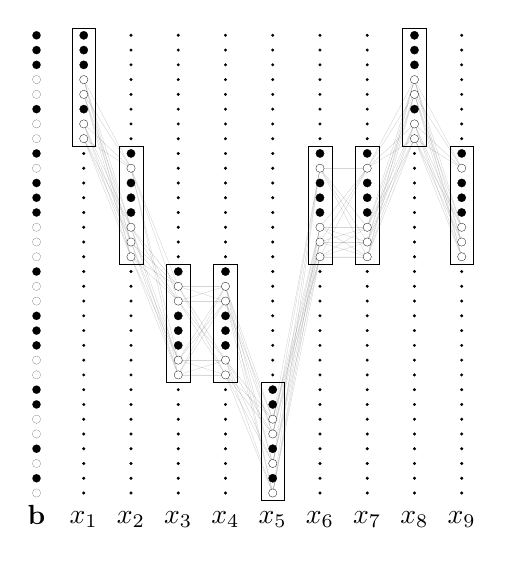
\begin{tikzpicture}%
\path[draw,line width=0.01pt,fill=white,radius=1.5pt] (0.0,0.0) circle;%
\path[draw,line width=0.01pt,fill=black,radius=1.5pt] (0.0,0.1875) circle;%
\path[draw,line width=0.01pt,fill=white,radius=1.5pt] (0.0,0.375) circle;%
\path[draw,line width=0.01pt,fill=black,radius=1.5pt] (0.0,0.5625) circle;%
\path[draw,line width=0.01pt,fill=white,radius=1.5pt] (0.0,0.75) circle;%
\path[draw,line width=0.01pt,fill=white,radius=1.5pt] (0.0,0.9375) circle;%
\path[draw,line width=0.01pt,fill=black,radius=1.5pt] (0.0,1.125) circle;%
\path[draw,line width=0.01pt,fill=black,radius=1.5pt] (0.0,1.3125) circle;%
\path[draw,line width=0.01pt,fill=white,radius=1.5pt] (0.0,1.5) circle;%
\path[draw,line width=0.01pt,fill=white,radius=1.5pt] (0.0,1.6875) circle;%
\path[draw,line width=0.01pt,fill=black,radius=1.5pt] (0.0,1.875) circle;%
\path[draw,line width=0.01pt,fill=black,radius=1.5pt] (0.0,2.0625) circle;%
\path[draw,line width=0.01pt,fill=black,radius=1.5pt] (0.0,2.25) circle;%
\path[draw,line width=0.01pt,fill=white,radius=1.5pt] (0.0,2.4375) circle;%
\path[draw,line width=0.01pt,fill=white,radius=1.5pt] (0.0,2.625) circle;%
\path[draw,line width=0.01pt,fill=black,radius=1.5pt] (0.0,2.8125) circle;%
\path[draw,line width=0.01pt,fill=white,radius=1.5pt] (0.0,3.0) circle;%
\path[draw,line width=0.01pt,fill=white,radius=1.5pt] (0.0,3.1875) circle;%
\path[draw,line width=0.01pt,fill=white,radius=1.5pt] (0.0,3.375) circle;%
\path[draw,line width=0.01pt,fill=black,radius=1.5pt] (0.0,3.5625) circle;%
\path[draw,line width=0.01pt,fill=black,radius=1.5pt] (0.0,3.75) circle;%
\path[draw,line width=0.01pt,fill=black,radius=1.5pt] (0.0,3.9375) circle;%
\path[draw,line width=0.01pt,fill=white,radius=1.5pt] (0.0,4.125) circle;%
\path[draw,line width=0.01pt,fill=black,radius=1.5pt] (0.0,4.3125) circle;%
\path[draw,line width=0.01pt,fill=white,radius=1.5pt] (0.0,4.5) circle;%
\path[draw,line width=0.01pt,fill=white,radius=1.5pt] (0.0,4.6875) circle;%
\path[draw,line width=0.01pt,fill=black,radius=1.5pt] (0.0,4.875) circle;%
\path[draw,line width=0.01pt,fill=white,radius=1.5pt] (0.0,5.0625) circle;%
\path[draw,line width=0.01pt,fill=white,radius=1.5pt] (0.0,5.25) circle;%
\path[draw,line width=0.01pt,fill=black,radius=1.5pt] (0.0,5.4375) circle;%
\path[draw,line width=0.01pt,fill=black,radius=1.5pt] (0.0,5.625) circle;%
\path[draw,line width=0.01pt,fill=black,radius=1.5pt] (0.0,5.8125) circle;%
\path[draw,line width=0.1pt,opacity=0.15,fill=black] (0.6,4.5) -- (1.2,3.0);%
\path[draw,line width=0.1pt,opacity=0.15,fill=black] (0.6,4.5) -- (1.2,3.1875);%
\path[draw,line width=0.1pt,opacity=0.15,fill=black] (0.6,4.5) -- (1.2,3.375);%
\path[draw,line width=0.1pt,opacity=0.15,fill=black] (0.6,4.5) -- (1.2,4.125);%
\path[draw,line width=0.1pt,opacity=0.15,fill=black] (0.6,4.6875) -- (1.2,3.0);%
\path[draw,line width=0.1pt,opacity=0.15,fill=black] (0.6,4.6875) -- (1.2,3.1875);%
\path[draw,line width=0.1pt,opacity=0.15,fill=black] (0.6,4.6875) -- (1.2,3.375);%
\path[draw,line width=0.1pt,opacity=0.15,fill=black] (0.6,4.6875) -- (1.2,4.125);%
\path[draw,line width=0.1pt,opacity=0.15,fill=black] (0.6,5.0625) -- (1.2,3.0);%
\path[draw,line width=0.1pt,opacity=0.15,fill=black] (0.6,5.0625) -- (1.2,3.1875);%
\path[draw,line width=0.1pt,opacity=0.15,fill=black] (0.6,5.0625) -- (1.2,3.375);%
\path[draw,line width=0.1pt,opacity=0.15,fill=black] (0.6,5.0625) -- (1.2,4.125);%
\path[draw,line width=0.1pt,opacity=0.15,fill=black] (0.6,5.25) -- (1.2,3.0);%
\path[draw,line width=0.1pt,opacity=0.15,fill=black] (0.6,5.25) -- (1.2,3.1875);%
\path[draw,line width=0.1pt,opacity=0.15,fill=black] (0.6,5.25) -- (1.2,3.375);%
\path[draw,line width=0.1pt,opacity=0.15,fill=black] (0.6,5.25) -- (1.2,4.125);%
\path[draw,line width=0.1pt,opacity=0.15,fill=black] (1.2,3.0) -- (1.8,1.5);%
\path[draw,line width=0.1pt,opacity=0.15,fill=black] (1.2,3.0) -- (1.8,1.6875);%
\path[draw,line width=0.1pt,opacity=0.15,fill=black] (1.2,3.0) -- (1.8,2.4375);%
\path[draw,line width=0.1pt,opacity=0.15,fill=black] (1.2,3.0) -- (1.8,2.625);%
\path[draw,line width=0.1pt,opacity=0.15,fill=black] (1.2,3.1875) -- (1.8,1.5);%
\path[draw,line width=0.1pt,opacity=0.15,fill=black] (1.2,3.1875) -- (1.8,1.6875);%
\path[draw,line width=0.1pt,opacity=0.15,fill=black] (1.2,3.1875) -- (1.8,2.4375);%
\path[draw,line width=0.1pt,opacity=0.15,fill=black] (1.2,3.1875) -- (1.8,2.625);%
\path[draw,line width=0.1pt,opacity=0.15,fill=black] (1.2,3.375) -- (1.8,1.5);%
\path[draw,line width=0.1pt,opacity=0.15,fill=black] (1.2,3.375) -- (1.8,1.6875);%
\path[draw,line width=0.1pt,opacity=0.15,fill=black] (1.2,3.375) -- (1.8,2.4375);%
\path[draw,line width=0.1pt,opacity=0.15,fill=black] (1.2,3.375) -- (1.8,2.625);%
\path[draw,line width=0.1pt,opacity=0.15,fill=black] (1.2,4.125) -- (1.8,1.5);%
\path[draw,line width=0.1pt,opacity=0.15,fill=black] (1.2,4.125) -- (1.8,1.6875);%
\path[draw,line width=0.1pt,opacity=0.15,fill=black] (1.2,4.125) -- (1.8,2.4375);%
\path[draw,line width=0.1pt,opacity=0.15,fill=black] (1.2,4.125) -- (1.8,2.625);%
\path[draw,line width=0.1pt,opacity=0.15,fill=black] (1.8,1.5) -- (2.4,1.5);%
\path[draw,line width=0.1pt,opacity=0.15,fill=black] (1.8,1.5) -- (2.4,1.6875);%
\path[draw,line width=0.1pt,opacity=0.15,fill=black] (1.8,1.5) -- (2.4,2.4375);%
\path[draw,line width=0.1pt,opacity=0.15,fill=black] (1.8,1.5) -- (2.4,2.625);%
\path[draw,line width=0.1pt,opacity=0.15,fill=black] (1.8,1.6875) -- (2.4,1.5);%
\path[draw,line width=0.1pt,opacity=0.15,fill=black] (1.8,1.6875) -- (2.4,1.6875);%
\path[draw,line width=0.1pt,opacity=0.15,fill=black] (1.8,1.6875) -- (2.4,2.4375);%
\path[draw,line width=0.1pt,opacity=0.15,fill=black] (1.8,1.6875) -- (2.4,2.625);%
\path[draw,line width=0.1pt,opacity=0.15,fill=black] (1.8,2.4375) -- (2.4,1.5);%
\path[draw,line width=0.1pt,opacity=0.15,fill=black] (1.8,2.4375) -- (2.4,1.6875);%
\path[draw,line width=0.1pt,opacity=0.15,fill=black] (1.8,2.4375) -- (2.4,2.4375);%
\path[draw,line width=0.1pt,opacity=0.15,fill=black] (1.8,2.4375) -- (2.4,2.625);%
\path[draw,line width=0.1pt,opacity=0.15,fill=black] (1.8,2.625) -- (2.4,1.5);%
\path[draw,line width=0.1pt,opacity=0.15,fill=black] (1.8,2.625) -- (2.4,1.6875);%
\path[draw,line width=0.1pt,opacity=0.15,fill=black] (1.8,2.625) -- (2.4,2.4375);%
\path[draw,line width=0.1pt,opacity=0.15,fill=black] (1.8,2.625) -- (2.4,2.625);%
\path[draw,line width=0.1pt,opacity=0.15,fill=black] (2.4,1.5) -- (3.0,0.0);%
\path[draw,line width=0.1pt,opacity=0.15,fill=black] (2.4,1.5) -- (3.0,0.375);%
\path[draw,line width=0.1pt,opacity=0.15,fill=black] (2.4,1.5) -- (3.0,0.75);%
\path[draw,line width=0.1pt,opacity=0.15,fill=black] (2.4,1.5) -- (3.0,0.9375);%
\path[draw,line width=0.1pt,opacity=0.15,fill=black] (2.4,1.6875) -- (3.0,0.0);%
\path[draw,line width=0.1pt,opacity=0.15,fill=black] (2.4,1.6875) -- (3.0,0.375);%
\path[draw,line width=0.1pt,opacity=0.15,fill=black] (2.4,1.6875) -- (3.0,0.75);%
\path[draw,line width=0.1pt,opacity=0.15,fill=black] (2.4,1.6875) -- (3.0,0.9375);%
\path[draw,line width=0.1pt,opacity=0.15,fill=black] (2.4,2.4375) -- (3.0,0.0);%
\path[draw,line width=0.1pt,opacity=0.15,fill=black] (2.4,2.4375) -- (3.0,0.375);%
\path[draw,line width=0.1pt,opacity=0.15,fill=black] (2.4,2.4375) -- (3.0,0.75);%
\path[draw,line width=0.1pt,opacity=0.15,fill=black] (2.4,2.4375) -- (3.0,0.9375);%
\path[draw,line width=0.1pt,opacity=0.15,fill=black] (2.4,2.625) -- (3.0,0.0);%
\path[draw,line width=0.1pt,opacity=0.15,fill=black] (2.4,2.625) -- (3.0,0.375);%
\path[draw,line width=0.1pt,opacity=0.15,fill=black] (2.4,2.625) -- (3.0,0.75);%
\path[draw,line width=0.1pt,opacity=0.15,fill=black] (2.4,2.625) -- (3.0,0.9375);%
\path[draw,line width=0.1pt,opacity=0.15,fill=black] (3.0,0.0) -- (3.6,3.0);%
\path[draw,line width=0.1pt,opacity=0.15,fill=black] (3.0,0.0) -- (3.6,3.1875);%
\path[draw,line width=0.1pt,opacity=0.15,fill=black] (3.0,0.0) -- (3.6,3.375);%
\path[draw,line width=0.1pt,opacity=0.15,fill=black] (3.0,0.0) -- (3.6,4.125);%
\path[draw,line width=0.1pt,opacity=0.15,fill=black] (3.0,0.375) -- (3.6,3.0);%
\path[draw,line width=0.1pt,opacity=0.15,fill=black] (3.0,0.375) -- (3.6,3.1875);%
\path[draw,line width=0.1pt,opacity=0.15,fill=black] (3.0,0.375) -- (3.6,3.375);%
\path[draw,line width=0.1pt,opacity=0.15,fill=black] (3.0,0.375) -- (3.6,4.125);%
\path[draw,line width=0.1pt,opacity=0.15,fill=black] (3.0,0.75) -- (3.6,3.0);%
\path[draw,line width=0.1pt,opacity=0.15,fill=black] (3.0,0.75) -- (3.6,3.1875);%
\path[draw,line width=0.1pt,opacity=0.15,fill=black] (3.0,0.75) -- (3.6,3.375);%
\path[draw,line width=0.1pt,opacity=0.15,fill=black] (3.0,0.75) -- (3.6,4.125);%
\path[draw,line width=0.1pt,opacity=0.15,fill=black] (3.0,0.9375) -- (3.6,3.0);%
\path[draw,line width=0.1pt,opacity=0.15,fill=black] (3.0,0.9375) -- (3.6,3.1875);%
\path[draw,line width=0.1pt,opacity=0.15,fill=black] (3.0,0.9375) -- (3.6,3.375);%
\path[draw,line width=0.1pt,opacity=0.15,fill=black] (3.0,0.9375) -- (3.6,4.125);%
\path[draw,line width=0.1pt,opacity=0.15,fill=black] (3.6,3.0) -- (4.2,3.0);%
\path[draw,line width=0.1pt,opacity=0.15,fill=black] (3.6,3.0) -- (4.2,3.1875);%
\path[draw,line width=0.1pt,opacity=0.15,fill=black] (3.6,3.0) -- (4.2,3.375);%
\path[draw,line width=0.1pt,opacity=0.15,fill=black] (3.6,3.0) -- (4.2,4.125);%
\path[draw,line width=0.1pt,opacity=0.15,fill=black] (3.6,3.1875) -- (4.2,3.0);%
\path[draw,line width=0.1pt,opacity=0.15,fill=black] (3.6,3.1875) -- (4.2,3.1875);%
\path[draw,line width=0.1pt,opacity=0.15,fill=black] (3.6,3.1875) -- (4.2,3.375);%
\path[draw,line width=0.1pt,opacity=0.15,fill=black] (3.6,3.1875) -- (4.2,4.125);%
\path[draw,line width=0.1pt,opacity=0.15,fill=black] (3.6,3.375) -- (4.2,3.0);%
\path[draw,line width=0.1pt,opacity=0.15,fill=black] (3.6,3.375) -- (4.2,3.1875);%
\path[draw,line width=0.1pt,opacity=0.15,fill=black] (3.6,3.375) -- (4.2,3.375);%
\path[draw,line width=0.1pt,opacity=0.15,fill=black] (3.6,3.375) -- (4.2,4.125);%
\path[draw,line width=0.1pt,opacity=0.15,fill=black] (3.6,4.125) -- (4.2,3.0);%
\path[draw,line width=0.1pt,opacity=0.15,fill=black] (3.6,4.125) -- (4.2,3.1875);%
\path[draw,line width=0.1pt,opacity=0.15,fill=black] (3.6,4.125) -- (4.2,3.375);%
\path[draw,line width=0.1pt,opacity=0.15,fill=black] (3.6,4.125) -- (4.2,4.125);%
\path[draw,line width=0.1pt,opacity=0.15,fill=black] (4.2,3.0) -- (4.8,4.5);%
\path[draw,line width=0.1pt,opacity=0.15,fill=black] (4.2,3.0) -- (4.8,4.6875);%
\path[draw,line width=0.1pt,opacity=0.15,fill=black] (4.2,3.0) -- (4.8,5.0625);%
\path[draw,line width=0.1pt,opacity=0.15,fill=black] (4.2,3.0) -- (4.8,5.25);%
\path[draw,line width=0.1pt,opacity=0.15,fill=black] (4.2,3.1875) -- (4.8,4.5);%
\path[draw,line width=0.1pt,opacity=0.15,fill=black] (4.2,3.1875) -- (4.8,4.6875);%
\path[draw,line width=0.1pt,opacity=0.15,fill=black] (4.2,3.1875) -- (4.8,5.0625);%
\path[draw,line width=0.1pt,opacity=0.15,fill=black] (4.2,3.1875) -- (4.8,5.25);%
\path[draw,line width=0.1pt,opacity=0.15,fill=black] (4.2,3.375) -- (4.8,4.5);%
\path[draw,line width=0.1pt,opacity=0.15,fill=black] (4.2,3.375) -- (4.8,4.6875);%
\path[draw,line width=0.1pt,opacity=0.15,fill=black] (4.2,3.375) -- (4.8,5.0625);%
\path[draw,line width=0.1pt,opacity=0.15,fill=black] (4.2,3.375) -- (4.8,5.25);%
\path[draw,line width=0.1pt,opacity=0.15,fill=black] (4.2,4.125) -- (4.8,4.5);%
\path[draw,line width=0.1pt,opacity=0.15,fill=black] (4.2,4.125) -- (4.8,4.6875);%
\path[draw,line width=0.1pt,opacity=0.15,fill=black] (4.2,4.125) -- (4.8,5.0625);%
\path[draw,line width=0.1pt,opacity=0.15,fill=black] (4.2,4.125) -- (4.8,5.25);%
\path[draw,line width=0.1pt,opacity=0.15,fill=black] (4.8,4.5) -- (5.4,3.0);%
\path[draw,line width=0.1pt,opacity=0.15,fill=black] (4.8,4.5) -- (5.4,3.1875);%
\path[draw,line width=0.1pt,opacity=0.15,fill=black] (4.8,4.5) -- (5.4,3.375);%
\path[draw,line width=0.1pt,opacity=0.15,fill=black] (4.8,4.5) -- (5.4,4.125);%
\path[draw,line width=0.1pt,opacity=0.15,fill=black] (4.8,4.6875) -- (5.4,3.0);%
\path[draw,line width=0.1pt,opacity=0.15,fill=black] (4.8,4.6875) -- (5.4,3.1875);%
\path[draw,line width=0.1pt,opacity=0.15,fill=black] (4.8,4.6875) -- (5.4,3.375);%
\path[draw,line width=0.1pt,opacity=0.15,fill=black] (4.8,4.6875) -- (5.4,4.125);%
\path[draw,line width=0.1pt,opacity=0.15,fill=black] (4.8,5.0625) -- (5.4,3.0);%
\path[draw,line width=0.1pt,opacity=0.15,fill=black] (4.8,5.0625) -- (5.4,3.1875);%
\path[draw,line width=0.1pt,opacity=0.15,fill=black] (4.8,5.0625) -- (5.4,3.375);%
\path[draw,line width=0.1pt,opacity=0.15,fill=black] (4.8,5.0625) -- (5.4,4.125);%
\path[draw,line width=0.1pt,opacity=0.15,fill=black] (4.8,5.25) -- (5.4,3.0);%
\path[draw,line width=0.1pt,opacity=0.15,fill=black] (4.8,5.25) -- (5.4,3.1875);%
\path[draw,line width=0.1pt,opacity=0.15,fill=black] (4.8,5.25) -- (5.4,3.375);%
\path[draw,line width=0.1pt,opacity=0.15,fill=black] (4.8,5.25) -- (5.4,4.125);%
\path[draw,line width=0.2pt] (0.45,4.40625) rectangle (0.75,5.90625);%
\path[draw,line width=0.2pt] (1.05,2.90625) rectangle (1.35,4.40625);%
\path[draw,line width=0.2pt] (1.65,1.40625) rectangle (1.95,2.90625);%
\path[draw,line width=0.2pt] (2.25,1.40625) rectangle (2.55,2.90625);%
\path[draw,line width=0.2pt] (2.85,-0.09375) rectangle (3.15,1.40625);%
\path[draw,line width=0.2pt] (3.45,2.90625) rectangle (3.75,4.40625);%
\path[draw,line width=0.2pt] (4.05,2.90625) rectangle (4.35,4.40625);%
\path[draw,line width=0.2pt] (4.65,4.40625) rectangle (4.95,5.90625);%
\path[draw,line width=0.2pt] (5.25,2.90625) rectangle (5.55,4.40625);%
\node[inner sep=0] (b) at (0.0,-0.28125) {$\mathbf{b}$};%
\node (x1) at (0.6,-0.3375) {$x_1$};%
\node (x2) at (1.2,-0.3375) {$x_2$};%
\node (x3) at (1.8,-0.3375) {$x_3$};%
\node (x4) at (2.4,-0.3375) {$x_4$};%
\node (x5) at (3.0,-0.3375) {$x_5$};%
\node (x6) at (3.6,-0.3375) {$x_6$};%
\node (x7) at (4.2,-0.3375) {$x_7$};%
\node (x8) at (4.8,-0.3375) {$x_8$};%
\node (x9) at (5.4,-0.3375) {$x_9$};%
\path[draw,line width=0.1pt,fill=black,radius=0.5pt] (0.6,0.0) circle;%
\path[draw,line width=0.1pt,fill=black,radius=0.5pt] (0.6,0.1875) circle;%
\path[draw,line width=0.1pt,fill=black,radius=0.5pt] (0.6,0.375) circle;%
\path[draw,line width=0.1pt,fill=black,radius=0.5pt] (0.6,0.5625) circle;%
\path[draw,line width=0.1pt,fill=black,radius=0.5pt] (0.6,0.75) circle;%
\path[draw,line width=0.1pt,fill=black,radius=0.5pt] (0.6,0.9375) circle;%
\path[draw,line width=0.1pt,fill=black,radius=0.5pt] (0.6,1.125) circle;%
\path[draw,line width=0.1pt,fill=black,radius=0.5pt] (0.6,1.3125) circle;%
\path[draw,line width=0.1pt,fill=black,radius=0.5pt] (0.6,1.5) circle;%
\path[draw,line width=0.1pt,fill=black,radius=0.5pt] (0.6,1.6875) circle;%
\path[draw,line width=0.1pt,fill=black,radius=0.5pt] (0.6,1.875) circle;%
\path[draw,line width=0.1pt,fill=black,radius=0.5pt] (0.6,2.0625) circle;%
\path[draw,line width=0.1pt,fill=black,radius=0.5pt] (0.6,2.25) circle;%
\path[draw,line width=0.1pt,fill=black,radius=0.5pt] (0.6,2.4375) circle;%
\path[draw,line width=0.1pt,fill=black,radius=0.5pt] (0.6,2.625) circle;%
\path[draw,line width=0.1pt,fill=black,radius=0.5pt] (0.6,2.8125) circle;%
\path[draw,line width=0.1pt,fill=black,radius=0.5pt] (0.6,3.0) circle;%
\path[draw,line width=0.1pt,fill=black,radius=0.5pt] (0.6,3.1875) circle;%
\path[draw,line width=0.1pt,fill=black,radius=0.5pt] (0.6,3.375) circle;%
\path[draw,line width=0.1pt,fill=black,radius=0.5pt] (0.6,3.5625) circle;%
\path[draw,line width=0.1pt,fill=black,radius=0.5pt] (0.6,3.75) circle;%
\path[draw,line width=0.1pt,fill=black,radius=0.5pt] (0.6,3.9375) circle;%
\path[draw,line width=0.1pt,fill=black,radius=0.5pt] (0.6,4.125) circle;%
\path[draw,line width=0.1pt,fill=black,radius=0.5pt] (0.6,4.3125) circle;%
\path[draw,line width=0.1pt,fill=white,radius=1.5pt] (0.6,4.5) circle;%
\path[draw,line width=0.1pt,fill=white,radius=1.5pt] (0.6,4.6875) circle;%
\path[draw,line width=0.1pt,fill=black,radius=1.5pt] (0.6,4.875) circle;%
\path[draw,line width=0.1pt,fill=white,radius=1.5pt] (0.6,5.0625) circle;%
\path[draw,line width=0.1pt,fill=white,radius=1.5pt] (0.6,5.25) circle;%
\path[draw,line width=0.1pt,fill=black,radius=1.5pt] (0.6,5.4375) circle;%
\path[draw,line width=0.1pt,fill=black,radius=1.5pt] (0.6,5.625) circle;%
\path[draw,line width=0.1pt,fill=black,radius=1.5pt] (0.6,5.8125) circle;%
\path[draw,line width=0.1pt,fill=black,radius=0.5pt] (1.2,0.0) circle;%
\path[draw,line width=0.1pt,fill=black,radius=0.5pt] (1.2,0.1875) circle;%
\path[draw,line width=0.1pt,fill=black,radius=0.5pt] (1.2,0.375) circle;%
\path[draw,line width=0.1pt,fill=black,radius=0.5pt] (1.2,0.5625) circle;%
\path[draw,line width=0.1pt,fill=black,radius=0.5pt] (1.2,0.75) circle;%
\path[draw,line width=0.1pt,fill=black,radius=0.5pt] (1.2,0.9375) circle;%
\path[draw,line width=0.1pt,fill=black,radius=0.5pt] (1.2,1.125) circle;%
\path[draw,line width=0.1pt,fill=black,radius=0.5pt] (1.2,1.3125) circle;%
\path[draw,line width=0.1pt,fill=black,radius=0.5pt] (1.2,1.5) circle;%
\path[draw,line width=0.1pt,fill=black,radius=0.5pt] (1.2,1.6875) circle;%
\path[draw,line width=0.1pt,fill=black,radius=0.5pt] (1.2,1.875) circle;%
\path[draw,line width=0.1pt,fill=black,radius=0.5pt] (1.2,2.0625) circle;%
\path[draw,line width=0.1pt,fill=black,radius=0.5pt] (1.2,2.25) circle;%
\path[draw,line width=0.1pt,fill=black,radius=0.5pt] (1.2,2.4375) circle;%
\path[draw,line width=0.1pt,fill=black,radius=0.5pt] (1.2,2.625) circle;%
\path[draw,line width=0.1pt,fill=black,radius=0.5pt] (1.2,2.8125) circle;%
\path[draw,line width=0.1pt,fill=white,radius=1.5pt] (1.2,3.0) circle;%
\path[draw,line width=0.1pt,fill=white,radius=1.5pt] (1.2,3.1875) circle;%
\path[draw,line width=0.1pt,fill=white,radius=1.5pt] (1.2,3.375) circle;%
\path[draw,line width=0.1pt,fill=black,radius=1.5pt] (1.2,3.5625) circle;%
\path[draw,line width=0.1pt,fill=black,radius=1.5pt] (1.2,3.75) circle;%
\path[draw,line width=0.1pt,fill=black,radius=1.5pt] (1.2,3.9375) circle;%
\path[draw,line width=0.1pt,fill=white,radius=1.5pt] (1.2,4.125) circle;%
\path[draw,line width=0.1pt,fill=black,radius=1.5pt] (1.2,4.3125) circle;%
\path[draw,line width=0.1pt,fill=black,radius=0.5pt] (1.2,4.5) circle;%
\path[draw,line width=0.1pt,fill=black,radius=0.5pt] (1.2,4.6875) circle;%
\path[draw,line width=0.1pt,fill=black,radius=0.5pt] (1.2,4.875) circle;%
\path[draw,line width=0.1pt,fill=black,radius=0.5pt] (1.2,5.0625) circle;%
\path[draw,line width=0.1pt,fill=black,radius=0.5pt] (1.2,5.25) circle;%
\path[draw,line width=0.1pt,fill=black,radius=0.5pt] (1.2,5.4375) circle;%
\path[draw,line width=0.1pt,fill=black,radius=0.5pt] (1.2,5.625) circle;%
\path[draw,line width=0.1pt,fill=black,radius=0.5pt] (1.2,5.8125) circle;%
\path[draw,line width=0.1pt,fill=black,radius=0.5pt] (1.8,0.0) circle;%
\path[draw,line width=0.1pt,fill=black,radius=0.5pt] (1.8,0.1875) circle;%
\path[draw,line width=0.1pt,fill=black,radius=0.5pt] (1.8,0.375) circle;%
\path[draw,line width=0.1pt,fill=black,radius=0.5pt] (1.8,0.5625) circle;%
\path[draw,line width=0.1pt,fill=black,radius=0.5pt] (1.8,0.75) circle;%
\path[draw,line width=0.1pt,fill=black,radius=0.5pt] (1.8,0.9375) circle;%
\path[draw,line width=0.1pt,fill=black,radius=0.5pt] (1.8,1.125) circle;%
\path[draw,line width=0.1pt,fill=black,radius=0.5pt] (1.8,1.3125) circle;%
\path[draw,line width=0.1pt,fill=white,radius=1.5pt] (1.8,1.5) circle;%
\path[draw,line width=0.1pt,fill=white,radius=1.5pt] (1.8,1.6875) circle;%
\path[draw,line width=0.1pt,fill=black,radius=1.5pt] (1.8,1.875) circle;%
\path[draw,line width=0.1pt,fill=black,radius=1.5pt] (1.8,2.0625) circle;%
\path[draw,line width=0.1pt,fill=black,radius=1.5pt] (1.8,2.25) circle;%
\path[draw,line width=0.1pt,fill=white,radius=1.5pt] (1.8,2.4375) circle;%
\path[draw,line width=0.1pt,fill=white,radius=1.5pt] (1.8,2.625) circle;%
\path[draw,line width=0.1pt,fill=black,radius=1.5pt] (1.8,2.8125) circle;%
\path[draw,line width=0.1pt,fill=black,radius=0.5pt] (1.8,3.0) circle;%
\path[draw,line width=0.1pt,fill=black,radius=0.5pt] (1.8,3.1875) circle;%
\path[draw,line width=0.1pt,fill=black,radius=0.5pt] (1.8,3.375) circle;%
\path[draw,line width=0.1pt,fill=black,radius=0.5pt] (1.8,3.5625) circle;%
\path[draw,line width=0.1pt,fill=black,radius=0.5pt] (1.8,3.75) circle;%
\path[draw,line width=0.1pt,fill=black,radius=0.5pt] (1.8,3.9375) circle;%
\path[draw,line width=0.1pt,fill=black,radius=0.5pt] (1.8,4.125) circle;%
\path[draw,line width=0.1pt,fill=black,radius=0.5pt] (1.8,4.3125) circle;%
\path[draw,line width=0.1pt,fill=black,radius=0.5pt] (1.8,4.5) circle;%
\path[draw,line width=0.1pt,fill=black,radius=0.5pt] (1.8,4.6875) circle;%
\path[draw,line width=0.1pt,fill=black,radius=0.5pt] (1.8,4.875) circle;%
\path[draw,line width=0.1pt,fill=black,radius=0.5pt] (1.8,5.0625) circle;%
\path[draw,line width=0.1pt,fill=black,radius=0.5pt] (1.8,5.25) circle;%
\path[draw,line width=0.1pt,fill=black,radius=0.5pt] (1.8,5.4375) circle;%
\path[draw,line width=0.1pt,fill=black,radius=0.5pt] (1.8,5.625) circle;%
\path[draw,line width=0.1pt,fill=black,radius=0.5pt] (1.8,5.8125) circle;%
\path[draw,line width=0.1pt,fill=black,radius=0.5pt] (2.4,0.0) circle;%
\path[draw,line width=0.1pt,fill=black,radius=0.5pt] (2.4,0.1875) circle;%
\path[draw,line width=0.1pt,fill=black,radius=0.5pt] (2.4,0.375) circle;%
\path[draw,line width=0.1pt,fill=black,radius=0.5pt] (2.4,0.5625) circle;%
\path[draw,line width=0.1pt,fill=black,radius=0.5pt] (2.4,0.75) circle;%
\path[draw,line width=0.1pt,fill=black,radius=0.5pt] (2.4,0.9375) circle;%
\path[draw,line width=0.1pt,fill=black,radius=0.5pt] (2.4,1.125) circle;%
\path[draw,line width=0.1pt,fill=black,radius=0.5pt] (2.4,1.3125) circle;%
\path[draw,line width=0.1pt,fill=white,radius=1.5pt] (2.4,1.5) circle;%
\path[draw,line width=0.1pt,fill=white,radius=1.5pt] (2.4,1.6875) circle;%
\path[draw,line width=0.1pt,fill=black,radius=1.5pt] (2.4,1.875) circle;%
\path[draw,line width=0.1pt,fill=black,radius=1.5pt] (2.4,2.0625) circle;%
\path[draw,line width=0.1pt,fill=black,radius=1.5pt] (2.4,2.25) circle;%
\path[draw,line width=0.1pt,fill=white,radius=1.5pt] (2.4,2.4375) circle;%
\path[draw,line width=0.1pt,fill=white,radius=1.5pt] (2.4,2.625) circle;%
\path[draw,line width=0.1pt,fill=black,radius=1.5pt] (2.4,2.8125) circle;%
\path[draw,line width=0.1pt,fill=black,radius=0.5pt] (2.4,3.0) circle;%
\path[draw,line width=0.1pt,fill=black,radius=0.5pt] (2.4,3.1875) circle;%
\path[draw,line width=0.1pt,fill=black,radius=0.5pt] (2.4,3.375) circle;%
\path[draw,line width=0.1pt,fill=black,radius=0.5pt] (2.4,3.5625) circle;%
\path[draw,line width=0.1pt,fill=black,radius=0.5pt] (2.4,3.75) circle;%
\path[draw,line width=0.1pt,fill=black,radius=0.5pt] (2.4,3.9375) circle;%
\path[draw,line width=0.1pt,fill=black,radius=0.5pt] (2.4,4.125) circle;%
\path[draw,line width=0.1pt,fill=black,radius=0.5pt] (2.4,4.3125) circle;%
\path[draw,line width=0.1pt,fill=black,radius=0.5pt] (2.4,4.5) circle;%
\path[draw,line width=0.1pt,fill=black,radius=0.5pt] (2.4,4.6875) circle;%
\path[draw,line width=0.1pt,fill=black,radius=0.5pt] (2.4,4.875) circle;%
\path[draw,line width=0.1pt,fill=black,radius=0.5pt] (2.4,5.0625) circle;%
\path[draw,line width=0.1pt,fill=black,radius=0.5pt] (2.4,5.25) circle;%
\path[draw,line width=0.1pt,fill=black,radius=0.5pt] (2.4,5.4375) circle;%
\path[draw,line width=0.1pt,fill=black,radius=0.5pt] (2.4,5.625) circle;%
\path[draw,line width=0.1pt,fill=black,radius=0.5pt] (2.4,5.8125) circle;%
\path[draw,line width=0.1pt,fill=white,radius=1.5pt] (3.0,0.0) circle;%
\path[draw,line width=0.1pt,fill=black,radius=1.5pt] (3.0,0.1875) circle;%
\path[draw,line width=0.1pt,fill=white,radius=1.5pt] (3.0,0.375) circle;%
\path[draw,line width=0.1pt,fill=black,radius=1.5pt] (3.0,0.5625) circle;%
\path[draw,line width=0.1pt,fill=white,radius=1.5pt] (3.0,0.75) circle;%
\path[draw,line width=0.1pt,fill=white,radius=1.5pt] (3.0,0.9375) circle;%
\path[draw,line width=0.1pt,fill=black,radius=1.5pt] (3.0,1.125) circle;%
\path[draw,line width=0.1pt,fill=black,radius=1.5pt] (3.0,1.3125) circle;%
\path[draw,line width=0.1pt,fill=black,radius=0.5pt] (3.0,1.5) circle;%
\path[draw,line width=0.1pt,fill=black,radius=0.5pt] (3.0,1.6875) circle;%
\path[draw,line width=0.1pt,fill=black,radius=0.5pt] (3.0,1.875) circle;%
\path[draw,line width=0.1pt,fill=black,radius=0.5pt] (3.0,2.0625) circle;%
\path[draw,line width=0.1pt,fill=black,radius=0.5pt] (3.0,2.25) circle;%
\path[draw,line width=0.1pt,fill=black,radius=0.5pt] (3.0,2.4375) circle;%
\path[draw,line width=0.1pt,fill=black,radius=0.5pt] (3.0,2.625) circle;%
\path[draw,line width=0.1pt,fill=black,radius=0.5pt] (3.0,2.8125) circle;%
\path[draw,line width=0.1pt,fill=black,radius=0.5pt] (3.0,3.0) circle;%
\path[draw,line width=0.1pt,fill=black,radius=0.5pt] (3.0,3.1875) circle;%
\path[draw,line width=0.1pt,fill=black,radius=0.5pt] (3.0,3.375) circle;%
\path[draw,line width=0.1pt,fill=black,radius=0.5pt] (3.0,3.5625) circle;%
\path[draw,line width=0.1pt,fill=black,radius=0.5pt] (3.0,3.75) circle;%
\path[draw,line width=0.1pt,fill=black,radius=0.5pt] (3.0,3.9375) circle;%
\path[draw,line width=0.1pt,fill=black,radius=0.5pt] (3.0,4.125) circle;%
\path[draw,line width=0.1pt,fill=black,radius=0.5pt] (3.0,4.3125) circle;%
\path[draw,line width=0.1pt,fill=black,radius=0.5pt] (3.0,4.5) circle;%
\path[draw,line width=0.1pt,fill=black,radius=0.5pt] (3.0,4.6875) circle;%
\path[draw,line width=0.1pt,fill=black,radius=0.5pt] (3.0,4.875) circle;%
\path[draw,line width=0.1pt,fill=black,radius=0.5pt] (3.0,5.0625) circle;%
\path[draw,line width=0.1pt,fill=black,radius=0.5pt] (3.0,5.25) circle;%
\path[draw,line width=0.1pt,fill=black,radius=0.5pt] (3.0,5.4375) circle;%
\path[draw,line width=0.1pt,fill=black,radius=0.5pt] (3.0,5.625) circle;%
\path[draw,line width=0.1pt,fill=black,radius=0.5pt] (3.0,5.8125) circle;%
\path[draw,line width=0.1pt,fill=black,radius=0.5pt] (3.6,0.0) circle;%
\path[draw,line width=0.1pt,fill=black,radius=0.5pt] (3.6,0.1875) circle;%
\path[draw,line width=0.1pt,fill=black,radius=0.5pt] (3.6,0.375) circle;%
\path[draw,line width=0.1pt,fill=black,radius=0.5pt] (3.6,0.5625) circle;%
\path[draw,line width=0.1pt,fill=black,radius=0.5pt] (3.6,0.75) circle;%
\path[draw,line width=0.1pt,fill=black,radius=0.5pt] (3.6,0.9375) circle;%
\path[draw,line width=0.1pt,fill=black,radius=0.5pt] (3.6,1.125) circle;%
\path[draw,line width=0.1pt,fill=black,radius=0.5pt] (3.6,1.3125) circle;%
\path[draw,line width=0.1pt,fill=black,radius=0.5pt] (3.6,1.5) circle;%
\path[draw,line width=0.1pt,fill=black,radius=0.5pt] (3.6,1.6875) circle;%
\path[draw,line width=0.1pt,fill=black,radius=0.5pt] (3.6,1.875) circle;%
\path[draw,line width=0.1pt,fill=black,radius=0.5pt] (3.6,2.0625) circle;%
\path[draw,line width=0.1pt,fill=black,radius=0.5pt] (3.6,2.25) circle;%
\path[draw,line width=0.1pt,fill=black,radius=0.5pt] (3.6,2.4375) circle;%
\path[draw,line width=0.1pt,fill=black,radius=0.5pt] (3.6,2.625) circle;%
\path[draw,line width=0.1pt,fill=black,radius=0.5pt] (3.6,2.8125) circle;%
\path[draw,line width=0.1pt,fill=white,radius=1.5pt] (3.6,3.0) circle;%
\path[draw,line width=0.1pt,fill=white,radius=1.5pt] (3.6,3.1875) circle;%
\path[draw,line width=0.1pt,fill=white,radius=1.5pt] (3.6,3.375) circle;%
\path[draw,line width=0.1pt,fill=black,radius=1.5pt] (3.6,3.5625) circle;%
\path[draw,line width=0.1pt,fill=black,radius=1.5pt] (3.6,3.75) circle;%
\path[draw,line width=0.1pt,fill=black,radius=1.5pt] (3.6,3.9375) circle;%
\path[draw,line width=0.1pt,fill=white,radius=1.5pt] (3.6,4.125) circle;%
\path[draw,line width=0.1pt,fill=black,radius=1.5pt] (3.6,4.3125) circle;%
\path[draw,line width=0.1pt,fill=black,radius=0.5pt] (3.6,4.5) circle;%
\path[draw,line width=0.1pt,fill=black,radius=0.5pt] (3.6,4.6875) circle;%
\path[draw,line width=0.1pt,fill=black,radius=0.5pt] (3.6,4.875) circle;%
\path[draw,line width=0.1pt,fill=black,radius=0.5pt] (3.6,5.0625) circle;%
\path[draw,line width=0.1pt,fill=black,radius=0.5pt] (3.6,5.25) circle;%
\path[draw,line width=0.1pt,fill=black,radius=0.5pt] (3.6,5.4375) circle;%
\path[draw,line width=0.1pt,fill=black,radius=0.5pt] (3.6,5.625) circle;%
\path[draw,line width=0.1pt,fill=black,radius=0.5pt] (3.6,5.8125) circle;%
\path[draw,line width=0.1pt,fill=black,radius=0.5pt] (4.2,0.0) circle;%
\path[draw,line width=0.1pt,fill=black,radius=0.5pt] (4.2,0.1875) circle;%
\path[draw,line width=0.1pt,fill=black,radius=0.5pt] (4.2,0.375) circle;%
\path[draw,line width=0.1pt,fill=black,radius=0.5pt] (4.2,0.5625) circle;%
\path[draw,line width=0.1pt,fill=black,radius=0.5pt] (4.2,0.75) circle;%
\path[draw,line width=0.1pt,fill=black,radius=0.5pt] (4.2,0.9375) circle;%
\path[draw,line width=0.1pt,fill=black,radius=0.5pt] (4.2,1.125) circle;%
\path[draw,line width=0.1pt,fill=black,radius=0.5pt] (4.2,1.3125) circle;%
\path[draw,line width=0.1pt,fill=black,radius=0.5pt] (4.2,1.5) circle;%
\path[draw,line width=0.1pt,fill=black,radius=0.5pt] (4.2,1.6875) circle;%
\path[draw,line width=0.1pt,fill=black,radius=0.5pt] (4.2,1.875) circle;%
\path[draw,line width=0.1pt,fill=black,radius=0.5pt] (4.2,2.0625) circle;%
\path[draw,line width=0.1pt,fill=black,radius=0.5pt] (4.2,2.25) circle;%
\path[draw,line width=0.1pt,fill=black,radius=0.5pt] (4.2,2.4375) circle;%
\path[draw,line width=0.1pt,fill=black,radius=0.5pt] (4.2,2.625) circle;%
\path[draw,line width=0.1pt,fill=black,radius=0.5pt] (4.2,2.8125) circle;%
\path[draw,line width=0.1pt,fill=white,radius=1.5pt] (4.2,3.0) circle;%
\path[draw,line width=0.1pt,fill=white,radius=1.5pt] (4.2,3.1875) circle;%
\path[draw,line width=0.1pt,fill=white,radius=1.5pt] (4.2,3.375) circle;%
\path[draw,line width=0.1pt,fill=black,radius=1.5pt] (4.2,3.5625) circle;%
\path[draw,line width=0.1pt,fill=black,radius=1.5pt] (4.2,3.75) circle;%
\path[draw,line width=0.1pt,fill=black,radius=1.5pt] (4.2,3.9375) circle;%
\path[draw,line width=0.1pt,fill=white,radius=1.5pt] (4.2,4.125) circle;%
\path[draw,line width=0.1pt,fill=black,radius=1.5pt] (4.2,4.3125) circle;%
\path[draw,line width=0.1pt,fill=black,radius=0.5pt] (4.2,4.5) circle;%
\path[draw,line width=0.1pt,fill=black,radius=0.5pt] (4.2,4.6875) circle;%
\path[draw,line width=0.1pt,fill=black,radius=0.5pt] (4.2,4.875) circle;%
\path[draw,line width=0.1pt,fill=black,radius=0.5pt] (4.2,5.0625) circle;%
\path[draw,line width=0.1pt,fill=black,radius=0.5pt] (4.2,5.25) circle;%
\path[draw,line width=0.1pt,fill=black,radius=0.5pt] (4.2,5.4375) circle;%
\path[draw,line width=0.1pt,fill=black,radius=0.5pt] (4.2,5.625) circle;%
\path[draw,line width=0.1pt,fill=black,radius=0.5pt] (4.2,5.8125) circle;%
\path[draw,line width=0.1pt,fill=black,radius=0.5pt] (4.8,0.0) circle;%
\path[draw,line width=0.1pt,fill=black,radius=0.5pt] (4.8,0.1875) circle;%
\path[draw,line width=0.1pt,fill=black,radius=0.5pt] (4.8,0.375) circle;%
\path[draw,line width=0.1pt,fill=black,radius=0.5pt] (4.8,0.5625) circle;%
\path[draw,line width=0.1pt,fill=black,radius=0.5pt] (4.8,0.75) circle;%
\path[draw,line width=0.1pt,fill=black,radius=0.5pt] (4.8,0.9375) circle;%
\path[draw,line width=0.1pt,fill=black,radius=0.5pt] (4.8,1.125) circle;%
\path[draw,line width=0.1pt,fill=black,radius=0.5pt] (4.8,1.3125) circle;%
\path[draw,line width=0.1pt,fill=black,radius=0.5pt] (4.8,1.5) circle;%
\path[draw,line width=0.1pt,fill=black,radius=0.5pt] (4.8,1.6875) circle;%
\path[draw,line width=0.1pt,fill=black,radius=0.5pt] (4.8,1.875) circle;%
\path[draw,line width=0.1pt,fill=black,radius=0.5pt] (4.8,2.0625) circle;%
\path[draw,line width=0.1pt,fill=black,radius=0.5pt] (4.8,2.25) circle;%
\path[draw,line width=0.1pt,fill=black,radius=0.5pt] (4.8,2.4375) circle;%
\path[draw,line width=0.1pt,fill=black,radius=0.5pt] (4.8,2.625) circle;%
\path[draw,line width=0.1pt,fill=black,radius=0.5pt] (4.8,2.8125) circle;%
\path[draw,line width=0.1pt,fill=black,radius=0.5pt] (4.8,3.0) circle;%
\path[draw,line width=0.1pt,fill=black,radius=0.5pt] (4.8,3.1875) circle;%
\path[draw,line width=0.1pt,fill=black,radius=0.5pt] (4.8,3.375) circle;%
\path[draw,line width=0.1pt,fill=black,radius=0.5pt] (4.8,3.5625) circle;%
\path[draw,line width=0.1pt,fill=black,radius=0.5pt] (4.8,3.75) circle;%
\path[draw,line width=0.1pt,fill=black,radius=0.5pt] (4.8,3.9375) circle;%
\path[draw,line width=0.1pt,fill=black,radius=0.5pt] (4.8,4.125) circle;%
\path[draw,line width=0.1pt,fill=black,radius=0.5pt] (4.8,4.3125) circle;%
\path[draw,line width=0.1pt,fill=white,radius=1.5pt] (4.8,4.5) circle;%
\path[draw,line width=0.1pt,fill=white,radius=1.5pt] (4.8,4.6875) circle;%
\path[draw,line width=0.1pt,fill=black,radius=1.5pt] (4.8,4.875) circle;%
\path[draw,line width=0.1pt,fill=white,radius=1.5pt] (4.8,5.0625) circle;%
\path[draw,line width=0.1pt,fill=white,radius=1.5pt] (4.8,5.25) circle;%
\path[draw,line width=0.1pt,fill=black,radius=1.5pt] (4.8,5.4375) circle;%
\path[draw,line width=0.1pt,fill=black,radius=1.5pt] (4.8,5.625) circle;%
\path[draw,line width=0.1pt,fill=black,radius=1.5pt] (4.8,5.8125) circle;%
\path[draw,line width=0.1pt,fill=black,radius=0.5pt] (5.4,0.0) circle;%
\path[draw,line width=0.1pt,fill=black,radius=0.5pt] (5.4,0.1875) circle;%
\path[draw,line width=0.1pt,fill=black,radius=0.5pt] (5.4,0.375) circle;%
\path[draw,line width=0.1pt,fill=black,radius=0.5pt] (5.4,0.5625) circle;%
\path[draw,line width=0.1pt,fill=black,radius=0.5pt] (5.4,0.75) circle;%
\path[draw,line width=0.1pt,fill=black,radius=0.5pt] (5.4,0.9375) circle;%
\path[draw,line width=0.1pt,fill=black,radius=0.5pt] (5.4,1.125) circle;%
\path[draw,line width=0.1pt,fill=black,radius=0.5pt] (5.4,1.3125) circle;%
\path[draw,line width=0.1pt,fill=black,radius=0.5pt] (5.4,1.5) circle;%
\path[draw,line width=0.1pt,fill=black,radius=0.5pt] (5.4,1.6875) circle;%
\path[draw,line width=0.1pt,fill=black,radius=0.5pt] (5.4,1.875) circle;%
\path[draw,line width=0.1pt,fill=black,radius=0.5pt] (5.4,2.0625) circle;%
\path[draw,line width=0.1pt,fill=black,radius=0.5pt] (5.4,2.25) circle;%
\path[draw,line width=0.1pt,fill=black,radius=0.5pt] (5.4,2.4375) circle;%
\path[draw,line width=0.1pt,fill=black,radius=0.5pt] (5.4,2.625) circle;%
\path[draw,line width=0.1pt,fill=black,radius=0.5pt] (5.4,2.8125) circle;%
\path[draw,line width=0.1pt,fill=white,radius=1.5pt] (5.4,3.0) circle;%
\path[draw,line width=0.1pt,fill=white,radius=1.5pt] (5.4,3.1875) circle;%
\path[draw,line width=0.1pt,fill=white,radius=1.5pt] (5.4,3.375) circle;%
\path[draw,line width=0.1pt,fill=black,radius=1.5pt] (5.4,3.5625) circle;%
\path[draw,line width=0.1pt,fill=black,radius=1.5pt] (5.4,3.75) circle;%
\path[draw,line width=0.1pt,fill=black,radius=1.5pt] (5.4,3.9375) circle;%
\path[draw,line width=0.1pt,fill=white,radius=1.5pt] (5.4,4.125) circle;%
\path[draw,line width=0.1pt,fill=black,radius=1.5pt] (5.4,4.3125) circle;%
\path[draw,line width=0.1pt,fill=black,radius=0.5pt] (5.4,4.5) circle;%
\path[draw,line width=0.1pt,fill=black,radius=0.5pt] (5.4,4.6875) circle;%
\path[draw,line width=0.1pt,fill=black,radius=0.5pt] (5.4,4.875) circle;%
\path[draw,line width=0.1pt,fill=black,radius=0.5pt] (5.4,5.0625) circle;%
\path[draw,line width=0.1pt,fill=black,radius=0.5pt] (5.4,5.25) circle;%
\path[draw,line width=0.1pt,fill=black,radius=0.5pt] (5.4,5.4375) circle;%
\path[draw,line width=0.1pt,fill=black,radius=0.5pt] (5.4,5.625) circle;%
\path[draw,line width=0.1pt,fill=black,radius=0.5pt] (5.4,5.8125) circle;%
\end{tikzpicture}%

}
\caption{With state dropout}
\end{subfigure}
\end{center}
\end{figure}

\end{frame}

\begin{frame}
\frametitle{Method Recap}
\begin{itemize}
\item Compact neural parameterization
\vspace{1em}
    \begin{itemize}
    \item[] \FancyUpArrow~Generalization
    \end{itemize}
\vspace{1em}
\item State dropout
\vspace{1em}
    \begin{itemize}
    \item[] \FancyUpArrow~Speed \quad \FancyUpArrow~Generalization
    \end{itemize}
\vspace{1em}
\item Block-sparse emission constraints
\vspace{1em}
    \begin{itemize}
    \item[] \FancyUpArrow~Speed
    \end{itemize}
\vspace{1em}
\item A fourth after experiments
\end{itemize}
\end{frame}


\section{Experiments}
\begin{frame}
\frametitle{Experiments}
\begin{itemize}
\item Language modeling on Penn Treebank
\vspace{1em}
\item Evaluate perplexity
    \begin{itemize}
    \item Function of $p(x)$
    \item Lower is better
    \end{itemize}
\vspace{1em}
\item Baselines
    \begin{itemize}
    \item Feedforward 5-gram model
    \item 2-layer LSTM
    \item A 900 state HMM\footcite{buys2018hmm}
    \end{itemize}
\vspace{1em}
\item Model
    \begin{itemize}
    \item $2^{15}$ (32k) state spare emission HMM (SE-HMM)
    \item $M=128$ groups (256 states per type), obtained via Brown Clustering
    \item Dropout rate of $0.5$ during training
    \end{itemize}
\end{itemize}
\end{frame}

\begin{frame}
\frametitle{Results on PTB Validation Data}
\centering
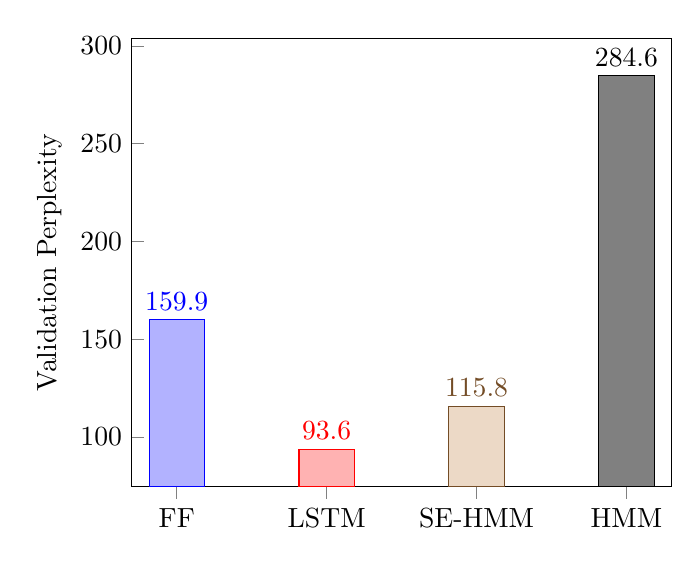
\begin{tikzpicture}
\begin{axis}[
    ybar=5pt,
    %x=4cm,
    %enlarge x limits=0.6,
    ylabel={Validation Perplexity},
    symbolic x coords={FF, LSTM, SE-HMM, HMM},
    xticklabels={FF, LSTM, SE-HMM, HMM},
    xtick={FF, LSTM, SE-HMM, HMM},
    tick pos=left,
    every axis plot/.append style={
      ybar,
      bar shift=0pt,
      fill
    },
    nodes near coords,
    nodes near coords align={vertical},
    bar width=2em,
    ]

\addplot coordinates {(FF,159.9)};
\addplot coordinates {(LSTM,93.6)};
\addplot coordinates {(SE-HMM,115.8)};
\addplot coordinates {(HMM,284.6)};

\end{axis}
\end{tikzpicture}
\end{frame}

\begin{frame}
\frametitle{State Size Ablation}

\centering
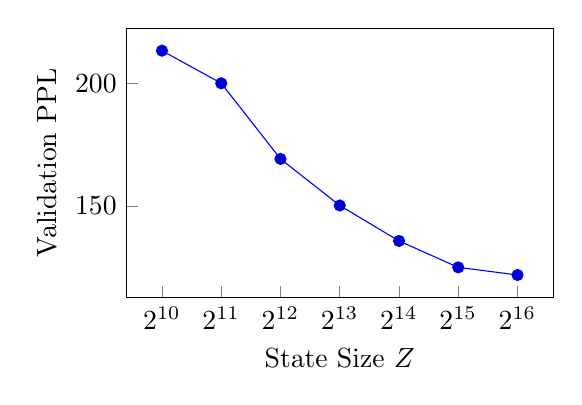
\begin{tikzpicture}
\begin{axis}[
    xlabel=State Size $Z$,
    ylabel=Validation PPL,
    xmode=log,
    log basis x={2},
    xtick={},
    tick pos=left,
    width=7cm,
    height=5cm
]
\addplot plot coordinates {
(1024,  213.25)
(2048,  199.98)
(4096,  169.18)
(8192,  150.22)
(16384, 135.79)
(32768, 125.02)
(65536, 121.93)
};
\end{axis}
\end{tikzpicture}

\vspace{2em}

Validation perplexity on PTB by state size ($\lambda =0.5$ and $M=128$)
\end{frame}

\begin{frame}
\frametitle{Other Ablations}

\begin{center}
\begin{tabular}{lrrr}
\toprule
Model                 & Param & Train & Val\\
\midrule
SE-HMM ($2^{14}$)     & 7.2M & 115    & 134 \\
\quad - neural param  & 423M & 119    & 169 \\
\quad - state dropout & 7.2M & 88     & 157 \\
%\quad + uniform partition & 7.2M & 83     & 145 \\
\bottomrule
\end{tabular}
\end{center}
\end{frame}

\begin{frame}
\frametitle{Discussion}
\begin{itemize}
\item Greatly scaled the state size of HMMs
\vspace{2em}
\item Performance improved with increasing state size
\vspace{2em}
\item Still a large gap between RNNs and HMMs
\vspace{2em}
\item Does the emission sparsity constraint improve
    computation complexity at the price of accuracy?
\end{itemize}
\end{frame}


\section{Speeding up HMMs with Low-Rank Factorizations\\{\normalsize A work in progress}}

\begin{frame}
\frametitle{Fast Inference with Low-Rank Factorizations}
\begin{itemize}
\item The previous approach relied a pre-specified emission sparsity constraint
\vspace{2em}
\item Can we scale inference with a weaker constraint?
\vspace{2em}
\item Exploit structure in the transition matrix to speed up inference
\end{itemize}
\end{frame}

\begin{frame}
\frametitle{Inference}
Start by unpacking inference to reveal the most expensive step

$$p(x) = \alpha_1^\top\Lambda_2\Lambda_3\cdots\Lambda_T\mathbf{1}$$
with
\begin{align*}
&\textnormal{start, } & [\alpha_1]_{z_1} &= p(x_1\mid z_1)p(z_1),\\
&\textnormal{and transition operators, }
    & [\Lambda_t]_{z_{t-1},z_t} &= p(x_t \mid z_t)p(z_t \mid z_{t-1})
\end{align*}
\end{frame}

\begin{frame}
\frametitle{Inference}
Decompose transition operators into transition matrix $A$ and emission matrix $O$
\begin{align*}
p(x) &= \alpha_1^\top\Lambda_2\cdot\Lambda_T\mathbf{1}\\
&= \alpha_1^\top (A \diag([O]_{\cdot,x_2}))  \cdots\Lambda_T\mathbf{1}\\
&= \alpha_1^\top A \diag([O]_{\cdot,x_2}) \cdots A \diag([O]_{\cdot,x_T}) \mathbf{1}
\end{align*}
where the most expensive steps are the matrix-vector products $\alpha_t^\top A$,
which take $O(Z^2)$ computation

\end{frame}

\begin{frame}
\frametitle{Fast Matrix-Vector Products}
\begin{itemize}
\item Goal is to reduce the naive matvec complexity of $O(Z^2)$
\vspace{1em}
\item Various methods
    \begin{itemize}
    \item Sparsity (nnz entries)
    \item Fast Fourier Transform ($Z \log Z$)
    \item Low-Rank factorization ($ZR$)
    \end{itemize}
\vspace{1em}
\item We utilize low-rank factorizations
\vspace{1em}
\item Connected to work in efficient attention and kernel approximations
\footcite{performer,rfa,blanc2018adaptive}
\end{itemize}
\end{frame}

\begin{frame}
\frametitle{Low-Rank Factorization}
Factor transitions $A\in[0,1]^{Z\times Z}$ into product of $U,V\in\R^{Z \times R}$
\[
\vcenter{\hbox{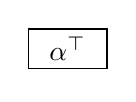
\begin{tikzpicture}[baseline=-0.5ex]
    \draw (0,0) rectangle (1,.5) node[pos=.5] {$\alpha^\top$};
\end{tikzpicture}}}
\times
\vcenter{\hbox{\begin{tikzpicture}[baseline=-0.5ex]
    \draw (0,0) rectangle (2,2) node[pos=.5] {$A$};
\end{tikzpicture}}}
=
\left(\,
\vcenter{\hbox{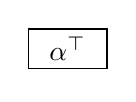
\begin{tikzpicture}[baseline=-0.5ex]
    \draw (0,0) rectangle (1,.5) node[pos=.5] {$\alpha^\top$};
\end{tikzpicture}}}
\times
\vcenter{\hbox{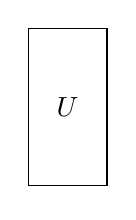
\begin{tikzpicture}[baseline=-0.5ex]
    \draw (0,0) rectangle (1,2) node[pos=.5] {$U$};
\end{tikzpicture}}}
\,\right)
\times 
\vcenter{\hbox{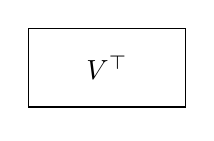
\begin{tikzpicture}[baseline=-0.5ex]
    \draw (0,0) rectangle (2,1) node[pos=.5] {$V^\top$};
\end{tikzpicture}}}
\]
resulting in two matrix-vector products of cost $O(ZR)$ each
\vspace{1em}
\begin{itemize}
\item Constraint: Entries of $A$ must be nonnegative
\vspace{1em}
\item Solution: Use a nonnegative matrix factorization (NMF)
$$A = \phi(U)\phi(V)^\top,$$
with $\phi:\R^{Z \times R}\to\R_+^{Z \times R}$
\end{itemize}
\end{frame}

\begin{frame}
\frametitle{Method Recap}
\begin{itemize}
\item Target key $O(Z^2)$ matvec step in inference
\vspace{2em}
\item Use NMF to reduce cost to $O(ZR)$
\vspace{2em}
\item How small can $R$ be relative to $Z$ without sacrificing accuracy?
\end{itemize}
\end{frame}


\section{Experiments}

\begin{frame}
\frametitle{Experiments}
\begin{itemize}
\item Language modeling on PTB
\vspace{2em}
\item Feature map $\phi(U) = \exp\left(U W\right)$,
with learned $W\in\R^{R \times R}$
\vspace{2em}
\item Baseline: Softmax HMM
\end{itemize}
\end{frame}

\begin{comment}
\begin{frame}
\frametitle{Asdf}
\begin{center}
\begin{figure}
\begin{subfigure}{0.49\textwidth}
    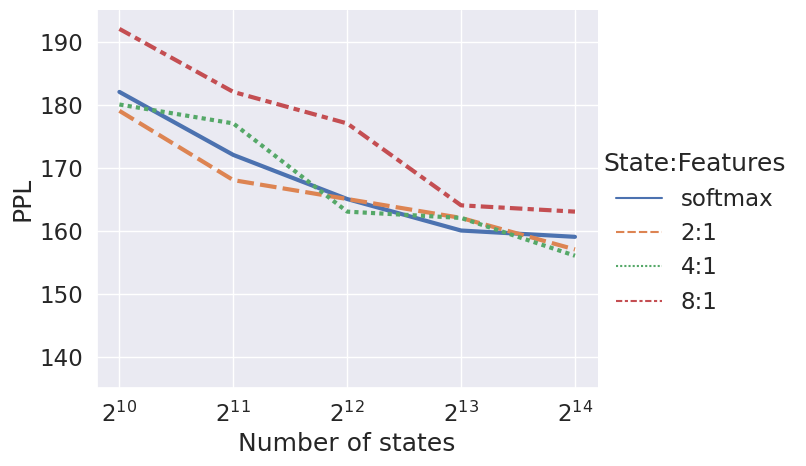
\includegraphics[width=\textwidth]{img/lhmm-states-features.png}
\end{subfigure}
\begin{subfigure}{0.49\textwidth}
    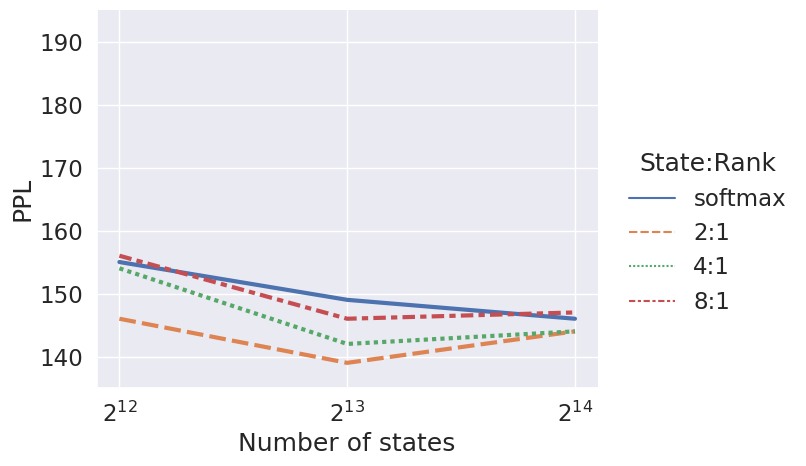
\includegraphics[width=\textwidth]{img/lhmm-states-features-dropout.png}
\end{subfigure}
\end{figure}
\end{center}
\end{frame}
\end{comment}

\begin{frame}
\frametitle{Scaling on PTB (Validation)}
\begin{center}
\begin{figure}
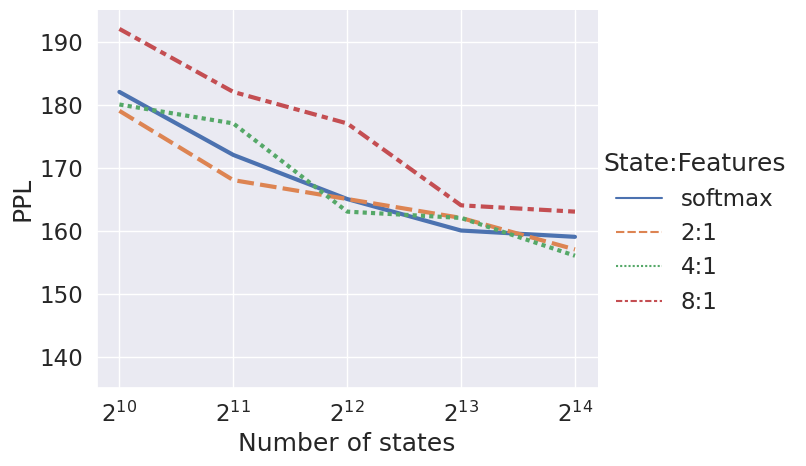
\includegraphics[width=\textwidth]{img/lhmm-states-features.png}
\end{figure}
\end{center}
\end{frame}

\begin{frame}
\frametitle{Further Scaling on PTB with Dropout (Validation)}
\begin{center}
\begin{figure}
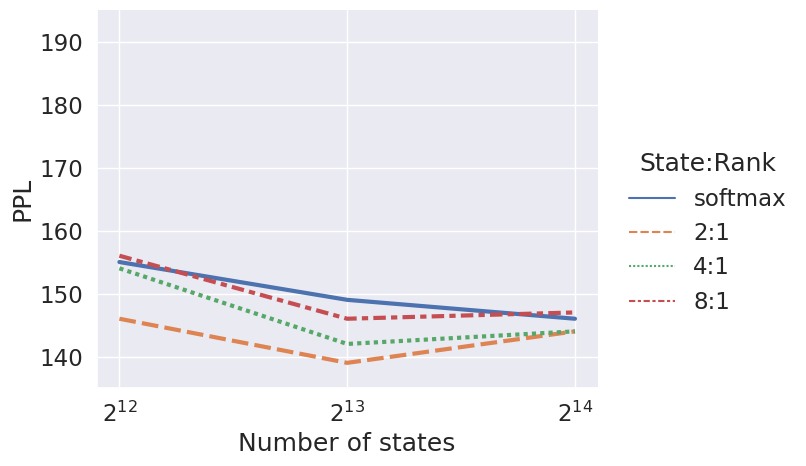
\includegraphics[width=\textwidth]{img/lhmm-states-features-dropout.png}
\end{figure}
\end{center}
\end{frame}

\begin{frame}
\frametitle{Speed Comparison\footnote{$2^{14}$ (16k) state SE-HMM takes 506 s/epoch on the same data}}
\begin{center}
\begin{figure}
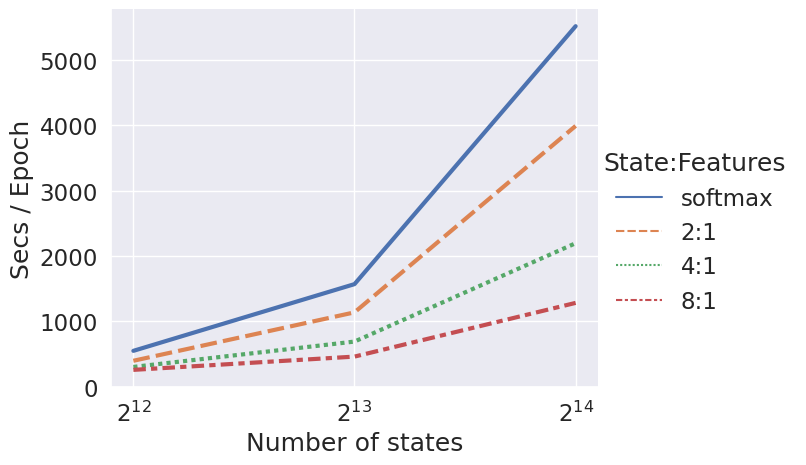
\includegraphics[width=\textwidth]{img/lhmm-states-features-speed.png}
\end{figure}
\end{center}
\end{frame}

\begin{frame}
\frametitle{Discussion}
\begin{itemize}
\item Reduced computation complexity of inference by 4x with NMF vs softmax HMM
\vspace{2em}
\item Scaling factor not as large as SE-HMM
\vspace{2em}
\item Validation PPL worse than SE-HMM
\end{itemize}
\end{frame}

\begin{frame}
\frametitle{Conclusion}
\begin{itemize}
\item Demonstrated improvements in perplexity with larger state spaces
\vspace{2em}
\item Extended techniques from neural networks to HMMs
\end{itemize}
\end{frame}

\begin{frame}
\frametitle{Future Work}
\begin{itemize}
\item Explore the performance of more complex interpretable models
    \begin{itemize}
    \item Probabilistic context-free grammars
    \item Switching linear dynamical systems\footcite{switch}
    \item Latent vector grammars\footcite{lveg}
    \end{itemize}
\item Explore other structure for fast matrix-vector products and tensor generalizations
    \begin{itemize}
    \item FFT-inspired algorithms\footcite{kal}
    \end{itemize}
\item Learn sparsity constraints in SE-HMM
\item Apply sparsity constraints to embedded HMMs\footcite{embhmm} for use in approximate inference
\end{itemize}
\end{frame}


\begin{frame}
\frametitle{EOS}
\end{frame}


\begin{frame}
\frametitle{Citations}
\printbibliography
%\bibliographystyle{acl_natbib}
%\bibliography{anthology,emnlp2020}
\end{frame}

\begin{frame}
\frametitle{Generalized Softmax}
\begin{itemize}
\item Softmax
$$p(z_t \mid z_{t-1}) = \frac{\exp(\bu_{z_{t-1}}^\top \bv_{z_{t}})}
{\sum_z \exp(\bu_{z_{t-1}}^\top \bv_z)}$$
\vspace{1em}
\item Generalized Softmax
$$p(z_t \mid z_{t-1})
= \frac{K(\bu, \bv)}{\sum_z K(\bu,\bv_z)}
= \frac{\phi(\bu)^\top\phi(\bv)}
    {\sum_z \phi(\bu)^\top\phi(\bv_z)},$$
for positive kernel $K:\R^D\times\R^D\to\R_+$
and feature map $\phi:\R^D\to\R^R$
\end{itemize}
\end{frame}

\begin{frame}
\frametitle{Generalized Softmax: Inference}
\begin{itemize}
\item The key $O(Z^2)$ step in the forward algorithm:
$$
p(z_t \mid x_{<t}) = \sum_{z_{t-1}} p(z_t \mid z_{t-1})p(z_{t-1} \mid x_{<t})
$$
\vspace{1em}
\item In matrix form, 
\begin{equation*}
\bm\gamma_t = \underbrace{\bm\alpha_{t-1}}_{\R^Z}\underbrace{\Lambda_{}}_{\R^{Z \times Z}},
\end{equation*}
where we have the probability of the
\begin{align*}
&\textnormal{current state, } & [\bm\gamma_{t}]_{z_{t}} &= p(z_{t} \mid x_{< t}),\\
&\textnormal{last state, } & [\bm\alpha_{t-1}]_{z_{t-1}} &= p(z_{t-1} \mid x_{< t}),\\
&\textnormal{transition probability, } & [\Lambda]_{z_{t-1},z_t} &= p(z_t\mid z_{t-1})
\end{align*}
\end{itemize}
\end{frame}

\begin{frame}
\frametitle{Generalized Softmax: Inference}
\begin{itemize}
\item Use generalized softmax in transition distribution
$$[\Lambda]_{z_{t-1},z_t} = p(z_t\mid z_{t-1}) \propto \phi(\bu_{z_{t-1}})^\top\phi(\bv_{z_t})$$
\item Allows us to apply associative property of matrix multiplication
\begin{align*}
\bm\gamma_t
&= \bm\alpha_{t-1}\Lambda\\
&= \bm\alpha_{t-1}(\textrm{diag}(d)\phi(U)\phi(V)^\top)\\
&= \underbrace{(\bm\alpha_{t-1}\circ d)}_{\R^Z}
\underbrace{\phi(U)}_{\R^{Z \times f}}
\underbrace{\phi(V)^\top}_{\R^{f \times Z}},
\end{align*}
with stacked embeddings $\phi(U),\phi(V) = [\phi(\bv_1), \ldots,\phi(\bv_Z)]$
and normalizing constants $d$
\vspace{1em}
\item Takes $O(Zf)$ time from left to right!
\end{itemize}
\end{frame}


\end{document}
